% \textenglish{This} \textenglish{LaTeX} \textenglish{document} \textenglish{needs} \textenglish{to} \textenglish{be} \textenglish{compiled} \textenglish{with} XeLaTeX.
\documentclass[10pt]{book}
\usepackage[utf8]{inputenc}
\usepackage{ucharclasses}
\usepackage{graphicx}
\usepackage[export]{adjustbox}
\graphicspath{ {./images/} }
\usepackage{hyperref}
\hypersetup{colorlinks=true, linkcolor=blue, filecolor=magenta, urlcolor=cyan,}
\urlstyle{same}
\usepackage{amsmath}
\usepackage{amsfonts}
\usepackage{amssymb}
\usepackage[version=4]{mhchem}
\usepackage{stmaryrd}
\usepackage{underscore}
\usepackage{fvextra, csquotes}
\usepackage{multirow}
\usepackage{polyglossia}
\usepackage{fontspec}
\usepackage{makeidx}
\makeindex
\setmainlanguage{english}
\setotherlanguages{bengali}
\IfFontExistsTF{Noto \textenglish{Serif} Bengali}
{\newfontfamily\bengalifont{Noto \textenglish{Serif} Bengali}}
{\IfFontExistsTF{Kohinoor Bangla}
  {\newfontfamily\bengalifont{Kohinoor Bangla}}
  {\IfFontExistsTF{Bangla MN}
    {\newfontfamily\bengalifont{Bangla MN}}
    {\IfFontExistsTF{Lohit Bengali}
      {\newfontfamily\bengalifont{Lohit Bengali}}
      {\IfFontExistsTF{FreeSerif}
        {\newfontfamily\bengalifont{FreeSerif}}
        {\newfontfamily\bengalifont{Arial \textenglish{Unicode} MS}}
}}}}
\IfFontExistsTF{CMU Serif}
{\newfontfamily\lgcfont{CMU Serif}}
{\IfFontExistsTF{DejaVu Sans}
  {\newfontfamily\lgcfont{DejaVu Sans}}
  {\newfontfamily\lgcfont{Georgia}}
}
\setDefaultTransitions{\lgcfont}{}
\setTransitionsFor{Bengali}{\bengalifont}{\lgcfont}

\title{कंप्यूटर विज्ञान में टेक्स्ट}

\author{स्टीवन एस. स्किना}



\maketitle

\tableofcontents

\chapter{प्रस्तावना}
हमारे आसपास की दुनिया को समझने के लिए हमें हमारे पर्यावरण से डेटा प्राप्त करना और उसका विश्लेषण करना आवश्यक है। हाल ही में कई प्रौद्योगिकी प्रवृत्तियाँ एक साथ आ गई हैं, जो हमें पहले से कहीं अधिक चुनौतीपूर्ण समस्याओं पर हमारे डेटा विश्लेषण कौशल को लागू करने के नए अवसर प्रदान करती हैं।

कंप्यूटर स्टोरेज क्षमता में अत्यधिक वृद्धि हुई है; वास्तव में याद रखना इतना सस्ता हो गया है कि कंप्यूटर सिस्टम को भूलने के लिए मजबूर करना लगभग असंभव हो गया है। सेंसरिंग उपकरण लगातार हर वह चीज़ मॉनिटर करते हैं जिसे देखा जा सकता है: वीडियो स्ट्रीम, सोशल मीडिया इंटरैक्शन, और कुछ भी जो चलता है उसकी स्थिति। क्लाउड कंप्यूटिंग हमें इस डेटा के मैनिपुलेशन के लिए बड़ी संख्या में मशीनों की शक्ति को संभालने में सक्षम बनाता है। वास्तव में, हर बार जब आप एक गूगल सर्च करते हैं तो सैकड़ों कंप्यूटर आपके सभी पिछले व्यवहार का गहराई से निरीक्षण करते हैं ताकि यह तय कर सकें कि अगले पर आपको कौन सा विज्ञापन दिखाना सबसे उपयुक्त है।

इस सब का परिणाम \textit{डेटा साइंस} का जन्म होना रहा है, जो जानकारी के विशाल संग्रहों से अधिकतम मूल्य प्राप्त करने के लिए समर्पित एक नया क्षेत्र है। ⸨डेटा साइंस⸩ एक अनुशासन के रूप में सांख्यिकी, कंप्यूटर साइंस, और मशीन लर्निंग के चौराहे पर कहीं स्थित है, लेकिन यह अपना खुद का एक विशिष्ट भार और चरित्र बना रहा है। यह पुस्तक ⸨डेटा साइंस⸩ के परिचय के रूप में कार्य करती है, जो उन कौशलों और सिद्धांतों पर केंद्रित है जो डेटा को एकत्रित, विश्लेषण और व्याख्या करने के लिए सिस्टम बनाने की आवश्यकता होती है।

मेरे पेशेवर अनुभव के आधार पर, एक शोधकर्ता और प्रशिक्षक के रूप में मुझे यह विश्वास होता है कि डेटा साइंस की एक बड़ी चुनौती यह है कि यह जितना दिखता है उससे कहीं अधिक सूक्ष्म है। कोई भी छात्र जिसने कभी अपना ग्रेड पॉइंट औसत (जीपीए) गणना किया हो, कहा जा सकता है कि उसने प्राथमिक सांख्यिकी की है, जैसे कि एक सरल स्कैटर प्लॉट बनाकर आप अपने रिज़्यूम में डेटा वीिज़ुअलाइज़ेशन का अनुभव जोड़ सकते हैं। लेकिन डेटा का अर्थपूर्ण विश्लेषण और व्याख्या करना तकनीकी विशेषज्ञता और बुद्धिमत्ता दोनों की आवश्यकता होती है। इतना अधिक लोग इन मूल बातों को इतने खराब तरीके से करते हैं, यही मेरी इस पुस्तक को लिखने की प्रेरणा प्रदान करता है।

\chapter{पाठक के लिए}
मुझे प्रसन्नता हुई है कि मेरी पुस्तक \textit{दि एल्गोरिदम डिज़ाइन मैनुअल} को 1997 में अपनी प्रारंभिक प्रकाशन के बाद से बहुत अच्छा प्रतिक्रिया मिला है। इसे एल्गोरिदमिक तकनीकों का उपयोग करके उन समस्याओं को हल करने के लिए एक अद्वितीय मार्गदर्शिका के रूप में मान्यता प्राप्त हुई है जो अक्सर व्यवहार में उत्पन्न होती हैं। जिस पुस्तक को आप पकड़े हुए हैं, वह बहुत अलग सामग्री को कवर करती है, लेकिन उसी प्रेरणा के साथ।

विशेष रूप से, यहाँ मैं एक अच्छे डेटा वैज्ञानिक बनने के लिए निम्नलिखित मूलभूत सिद्धांतों पर जोर देता हूँ:



साधारण का अर्थ आसान नहीं होता, हालांकि। वास्तव में सही प्रश्न पूछने और यह महसूस करने के लिए कि आप सही उत्तरों और कारगर अंतर्दृष्टि की ओर बढ़ रहे हैं, काफी सूझबूझ और अनुभव की आवश्यकता होती है। मैं यहां केवल इसलिए साफ, तकनीकी सामग्री में गहराई से जाने के प्रलोभन का विरोध करता हूँ क्योंकि यह सिखाने योग्य है। ऐसे कई अन्य पुस्तकें हैं जो मशीन लर्निंग अल्गॉरिदम्स या सांख्यिकीय परिकल्पना परीक्षण की जटिलताओं को कवर करेंगी। मेरा उद्देश्य यहाँ उन आधारभूत तत्वों को स्थापित करना है जो वास्तव में डेटा का विश्लेषण करने में मायने रखते हैं।

\item\textit{गणितीय अंतर्ज्ञान का विकास}: डेटा विज्ञान गणित की नींव पर टिका है, विशेष रूप से सांख्यिकी और रैखिक बीजगणित पर। इस सामग्री को अंतर्ज्ञान के स्तर पर समझना महत्वपूर्ण है: इन अवधारणाओं का विकास क्यों हुआ, ये कैसे उपयोगी हैं, और कब ये सबसे अच्छी तरह से काम करती हैं। मैं रैखिक बीजगणित में संचालन को चित्रित करने के लिए चित्र प्रस्तुत करता हूँ जो यह दिखाते हैं कि जब आप गणितीय सरणियों में हेरफेर करते हैं तो क्या होता है, और सांख्यिकीय अवधारणाओं को उदाहरणों और अवमूल्यन तर्कों के माध्यम से स्पष्ट करता हूँ। मेरा लक्ष्य यहाँ पाठक में अंतर्ज्ञान को प्रत्यारोपित करना है।

लेकिन मैं इस सामग्री को प्रस्तुत करने में औपचारिक गणित के उपयोग को कम से कम करने का प्रयास करता हूँ। वास्तव में, मैं इस पुस्तक में केवल एक औपचारिक प्रमाण प्रस्तुत करूँगा, एक गलत प्रमाण जहाँ संबंधित प्रमेय स्पष्ट रूप से गलत है। यहाँ नैतिकता यह नहीं है कि गणितीय कठोरता का कोई महत्व नहीं है, क्योंकि निश्चित रूप से ऐसा है, बल्कि यह है कि सच्ची कठोरता तब तक असंभव है जब तक समझ नहीं होती।

\item\textit{कंप्यूटर वैज्ञानिक की तरह सोचें, लेकिन सांख्यिकीविद् की तरह कार्य करें}: डेटा विज्ञान एक छत्र प्रदान करता है जो कंप्यूटर वैज्ञानिकों, सांख्यिकीविदों, और डोमेन विशेषज्ञों को जोड़ता है। लेकिन प्रत्येक समुदाय की अपनी अलग सोच और कार्य करने की शैलियाँ होती हैं, जो इसके सदस्यों की आत्माओं में अंकित हो जाती हैं।

इस पुस्तक में, मैं उन दृष्टिकोणों पर जोर देता हूँ जो कंप्यूटर विज्ञानी के लिए सबसे स्वाभाविक होते हैं, विशेष रूप से डेटा की एल्गोरिदमिक मैनिपुलेशन, मशीन लर्निंग का उपयोग, और पैमाने की महारत। लेकिन मैं सांख्यिकीय तर्कशक्ति के मूल्यों को भी संप्रेषित करने की कोशिश करता हूँ: आवेदन डोमेन को समझने की आवश्यकता, छोटे का उचित मूल्यांकन, महत्व की खोज और अन्वेषण की भूख।

कोई भी अनुशासन सत्य पर एकाधिकार नहीं रखता। सर्वश्रेष्ठ डेटा वैज्ञानिक विभिन्न क्षेत्रों के उपकरणों को सम्मिलित करते हैं, और यह किताब एक ऐसा अपेक्षाकृत तटस्थ क्षेत्र बनने का प्रयास करती है जहाँ प्रतिद्वंद्वी दार्शनिकताएं मिलकर तर्क-वितर्क कर सकें।

\end{itemize}

उतनी ही महत्वपूर्ण बात यह है कि आपको इस पुस्तक में क्या नहीं मिलेगा। मैं किसी विशेष भाषा या डाटा एनालिसिस टूल्स के सेट पर जोर नहीं देता। इसके बजाय, यह पुस्तक महत्वपूर्ण डिज़ाइन सिद्धांतों पर उच्च स्तर की चर्चा प्रदान करती है। मैं एक वैचारिक स्तर पर अधिक काम करने की कोशिश करता हूँ बजाय तकनीकी स्तर के। इस मैनुअल का लक्ष्य आपको जितना शीघ्र संभव हो सके सही दिशा में ले जाना है, उस सॉफ़्टवेयर टूल्स के साथ जो आपको सबसे अधिक सुलभ लगती हैं।

\chapter{शिक्षक के लिए}
यह पुस्तक स्नातक या प्रारंभिक स्नातकोत्तर छात्रों के स्तर पर \textit{डेटा साइंस का परिचय} पाठ्यक्रम के लिए पर्याप्त सामग्री को कवर करती है। मैं आशा करता हूँ कि पाठक ने कम से कम एक कार्यक्रमन पाठ्यक्रम के समकक्ष पूरा किया है और संभावना और सांख्यिकी का कुछ पूर्व अनुभव है, लेकिन हमेशा अधिक बेहतर होता है।

मैंने इस पाठ्यक्रम को पढ़ाने के लिए एक संपूर्ण व्याख्यान स्लाइड सेट ऑनलाइन उपलब्ध कराया है @। परियोजनाओं और असाइनमेंट्स के लिए डेटा संसाधन भी वहाँ पर उपलब्ध हैं जिससे प्रशिक्षक को सहायता मिल सके। इसके अलावा, मैं इन स्लाइड्स का उपयोग करके पूरे सेमेस्टर का डेटा साइंस पाठ्यक्रम पढ़ाने के लिए ऑनलाइन वीडियो व्याख्यान उपलब्ध कराता हूँ। वेब की जादू के माध्यम से अपनी कक्षा को पढ़ाने में मुझे मदद करने दीजिए!

इस पुस्तक की शैक्षिक विशेषताएँ शामिल हैं:



जवाब देने की बजाय, एक समाधान विकी सेट अप किया गया है, जहाँ हर दूसरे नंबर की समस्या के समाधान को सामूहिक योगदान द्वारा आमंत्रित किया जाएगा। मेरी\textit{एल्गोरिदम डिज़ाइन मैनुअल}के साथ एक समान प्रणाली ने संगठित समाधान उत्पन्न किए, या ऐसा मुझे बताया गया है। सिद्धांत के तौर पर मैं उन्हें देखने से इनकार करता हूँ, इसलिए खरीदार को सजग रहना चाहिए।
\item\textit{काग्ल चैलेंज}: काग्ल (\href{http://www.kaggle.com}{www.kaggle.com}) डाटा वैज्ञानिकों के लिए प्रतिस्पर्धा करने का मंच प्रदान करता है, जिसमें दिलचस्प डेटा सेट्स पर चुनौतीपूर्ण वास्तविक संसार की समस्याएँ शामिल होती हैं, और जो यह जांचते हैं कि आपका मॉडल अन्य प्रस्तुतियों की तुलना में कितना अच्छा है। प्रत्येक अध्याय के अभ्यास में तीन संबंधित काग्ल चैलेंज शामिल होते हैं, जो प्रेरणा का स्रोत, आत्म-अध्ययन, और अन्य परियोजनाओं और अन्वेषणों के लिए डेटा के रूप में काम करते हैं।\index{asking \textenglish{interesting} questions}\index{big \textenglish{data} engineer}\index{garbage in, \textenglish{garbage} out}\index{precision}\index{robustness}
\item\textit{डाटा साइंस टेलीविज़न}: डाटा साइंस आम जनता के लिए रहस्यमय और यहाँ तक कि डरावना भी बना हुआ है।\textit{द क्वांट शॉप}एक शौकिया प्रस्तुति है कि एक डाटा साइंस रियलिटी शो कैसा होना चाहिए। छात्र टीमें विभिन्न प्रकार की वास्तविक दुनिया की भविष्यवाणी समस्याओं से निपटती हैं, और भविष्य की घटनाओं के परिणाम की भविष्यवाणी करने की कोशिश करती हैं। इसे \href{http://www.quant-shop.com}{http://www.quant-shop.com} पर देखें।

आठ 30-मिनट एपिसोड की एक श्रृंखला तैयार की गई है, प्रत्येक को एक विशेष वास्तविक दुनिया की पूर्वानुमान समस्या के इर्द-गिर्द बनाया गया है। चुनौतियों में नीलामी में कला का मूल्य निर्धारण, मिस यूनिवर्स प्रतियोगिता के विजेता का चयन, और यह भविष्यवाणी करना शामिल है कि हस्तियाँ कब मरने वाली हैं। प्रत्येक के लिए, हम देखते हैं कि एक छात्र टीम समस्या से निपटती है, और उनके साथ सीखते हैं जैसे वे एक फोरकास्टिंग मॉडल बनाते हैं। वे अपने पूर्वानुमान बनाते हैं, और हम उनके साथ देखते हैं कि वे सही हैं या गलत।

इस पुस्तक में, \textit{द क्वांट शॉप} का उपयोग भविष्यवाणी चुनौतियों के ठोस उदाहरण प्रदान करने के लिए किया गया है, डेटा विज्ञान मॉडलिंग पाइपलाइन की चर्चाओं को डेटा अधिग्रहण से मूल्यांकन तक प्रारूपित करने के लिए। मुझे उम्मीद है कि आपको ये मजेदार लगेंगे, और ये आपके अपने मॉडलिंग चुनौतियों की कल्पना और उन्हें अपनाने के लिए प्रेरित करेंगे। 
\item\textit{अध्याय नोट्स}: अंततः, प्रत्येक ट्यूटोरियल अध्याय एक संक्षिप्त नोट्स अनुभाग के साथ समाप्त होता है, जो पाठकों को प्राथमिक स्रोतों और अतिरिक्त संदर्भों की ओर इंगित करता है। 
\end{itemize}

\chapter{समर्पण}
मेरी समझदार और प्यारी बेटियाँ बोननी और एबी अब पूरी तरह किशोरावस्था में हैं, जिसका मतलब है कि वे हमेशा सांख्यिकीय साक्ष्यों को उतनी तेजी से नहीं समझतीं जितना कि मैं चाहता हूँ। मैं यह पुस्तक उन्हें समर्पित करता हूँ, इस आशा में कि उनके विश्लेषण कौशल इस स्तर तक सुधारें कि वे हमेशा मुझसे सहमत रहें।

और मैं इस पुस्तक को अपनी सुंदर पत्नी ऱेनी को समर्पित करता हूं, जो मुझसे तब भी सहमत होती है जब वह मुझसे सहमत नहीं होती है, और जो मुझसे तब भी प्यार करती है जब सारे विश्वसनीय साक्ष्य मेरे पक्ष में नहीं होते।

\vfill
\noindent\textit{स्टीवन एस. स्कीना\\
कंप्यूटर साइंस विभाग\\
स्टोनी ब्रूक यूनिवर्सिटी\\
स्टोनी ब्रूक, एनवाई 11794-2424\\
\href{http://www.cs.stonybrook.edu/\~skiena}{http://www.cs.stonybrook.edu/\~skiena}\\
skiena@data-manual.com\\
मई 2017}

% \textenglish{Starting} \textenglish{off} \textenglish{the} \textenglish{main} \textenglish{matter} \textenglish{of} \textenglish{the} \textenglish{book} \textenglish{with} \textenglish{the} \textenglish{first} chapter\index{Barzun, Jacques}\index{major \textenglish{league} baseball}
\mainmatter

\chapter{डाटा साइंस क्या है?}
\textit{कंप्यूटिंग का उद्देश्य अंतर्दृष्टि है, संख्याएँ नहीं।}
--रिचर्ड डब्ल्यू हैमिंग

डेटा साइंस क्या है? किसी भी उभरते क्षेत्र की तरह, इसे अभी तक पूरी तरह से परिभाषित नहीं किया गया है, लेकिन आप इसके बारे में इतना जानते हैं कि रुचि रखते हों, अन्यथा आप यह पुस्तक नहीं पढ़ रहे होते।

मैं डाटा सायंस को कम्प्यूटर सायंस, सांख्यिकी, और वास्तविक अनुप्रयोग डोमेन के संगम पर स्थित मानता हूँ। कम्प्यूटर सायंस से मशीन लर्निंग और उच्च-प्रदर्शन कम्प्यूटिंग तकनीकें आती हैं जो बड़े पैमाने पर निपटने के लिए होती हैं। सांख्यिकी से खोजपूर्ण डाटा विश्लेषण, महत्व परीक्षण, और दृश्यता की एक लंबी परंपरा आती है। व्यवसाय और विज्ञान के अनुप्रयोग डोमेन से चुनौतियाँ आती हैं जो संघर्ष के योग्य होती हैं, और मूल्यांकन मानक जिनसे जांचा जाता है कि उन्हें कब पर्याप्त रूप से जीत लिया गया है।

लेकिन ये सभी अच्छी तरह से स्थापित क्षेत्र हैं। डेटा विज्ञान क्यों, और अभी क्यों? मैं इस अचानक सक्रियता के तीन कारण देखता हूँ:

\begin{itemize}
  \item नई तकनीक ने सोशल मीडिया, लॉगिंग और सेंसर डेटा की भारी मात्रा को कैप्चर, एनोटेट और स्टोर करना संभव बना दिया है। जब आपने ये सारा डेटा एकत्र कर लिया, तो आप यह सोचने लगते हैं कि इसके साथ आप क्या कर सकते हैं। 
  \item कंप्यूटिंग में प्रगति ने डेटा का विश्लेषण करने के लिए नई तरीकों और लगातार बढ़ते पैमाने पर इसे संभव बना दिया है। क्लाउड कंप्यूटिंग आर्किटेक्चर छोटे से छोटे व्यक्ति को भी आवश्यकता होने पर विशाल शक्ति तक पहुंच प्रदान करते हैं। मशीन लर्निंग के नए दृष्टिकोणों ने लंबे समय से बने समस्याओं जैसे कंप्यूटर विज़न और प्राकृतिक भाषा प्रसंस्करण में अद्भुत प्रगति लाई है। 
  \item प्रमुख तकनीकी कंपनियों (जैसे गूगल और फेसबुक) और क्वांटिटेटिव हेज फंड्स (जैसे रेनॉसांस टेक्नोलॉजीज और टू सिग्मा) ने आधुनिक डेटा एनालिटिक्स की शक्ति को साबित किया है। खेल प्रबंधन (\textit{Moneyball}) और चुनाव पूर्वानुमान (ने्ट सिल्वर) जैसे विविध क्षेत्रों में डेटा को लागू करने की सफलता की कहानियां डेटा विज्ञान को एक बड़े लोकप्रिय दर्शक तक लाने के लिए आदर्श मॉडल के रूप में काम आई हैं। 
\end{itemize}

यह परिचयात्मक अध्याय तीन मिशनों को प्रस्तुत करता है।पहला, मैं यह समझाने की कोशिश करूंगा कि अच्छे डाटा वैज्ञानिक कैसे सोचते हैं, और यह पारंपरिक प्रोग्रामर और सॉफ़्टवेयर डेवलपर की मानसिकता से कैसे अलग होता है। दूसरा, हम डेटा सेट्स को इस दृष्टिकोण से देखेंगे कि उन्हें किस-किस संभावनाओं के लिए उपयोग किया जा सकता है, और वे व्यापक प्रश्न पूछने की क्षमता रखते हैं।अंत में, मैं डेटा विश्लेषण की चुनौतियों का एक संग्रह प्रस्तुत करता हूँ जो इस पुस्तक में प्रेरणादायक उदाहरणों के रूप में इस्तेमाल होंगे।

\section{कंप्यूटर साइंस, डाटा साइंस, और रियल साइंस}
कंप्यूटर वैज्ञानिकों ने स्वाभाविक रूप से डाटा का सम्मान नहीं किया है। उन्हें पारंपरिक रूप से सिखाया गया था कि एल्गोरिदम वह चीज़ है, और डाटा सिर्फ एक सॉसेज ग्राइंडर के माध्यम से गुजारा जाने वाला मांस है।

इसलिए एक प्रभावी डेटा वैज्ञानिक के रूप में योग्य होने के लिए, आपको पहले एक वास्तविक वैज्ञानिक की तरह सोचना सीखना चाहिए। वास्तविक वैज्ञानिक प्राकृतिक दुनिया को समझने की कोशिश करते हैं, जो कि एक जटिल और अव्यवस्थित जगह है। इसके विपरीत, कंप्यूटर वैज्ञानिक अपनी स्वच्छ और सुव्यवस्थित आभासी दुनियाँ बनाते हैं और उनमें आराम से रहते हैं। वैज्ञानिक खोज करने के बारे में बहुत चिंतित रहते हैं, जबकि कंप्यूटर वैज्ञानिक खोज के बजाय आविष्कार करते हैं।

लोगों के मानसिक दृष्टिकोण यह वर्णित करते हैं कि वे कैसे सोचते हैं और कार्य करते हैं, जिससे तब गलतफहमियाँ होती हैं जब हम अपने समुदायों के बाहर संवाद करने की कोशिश करते हैं। ये पक्षपात इतने मौलिक होते हैं कि हमें अक्सर पता भी नहीं चलता कि ये हमारे पास हैं। कम्प्युटर साइंस और वास्तविक विज्ञान के बीच सांस्कृतिक भिन्नताओं के उदाहरणों में शामिल हैं:



इसके विपरीत, खराब कंप्यूटर वैज्ञानिक उन संख्याओं के बारे में चिंतित रहते हैं जो संभाव्य दिखती हैं। जैसे ही संख्याएँ अधिक गलत नहीं दिखतीं, उन्हें सही मान लिया जाता है। इसका कारण है कि वे व्यक्तिगत रूप से उस ज्ञान में कम निवेशित होते हैं जो कि किसी गणना से प्राप्त किया जा सकता है, इसके बजाय इसे जल्दी और कुशलता से पूरा करने में।
  
\item\textit{मजबूती}: वास्तविक वैज्ञानिक डेटा में त्रुटियों के विचार को सहजता से स्वीकार करते हैं। आम तौर पर, कंप्यूटर वैज्ञानिक ऐसा नहीं करते। वैज्ञानिक अपने डेटा में संभाव्य पूर्वाग्रह या त्रुटि के स्रोतों के बारे में बहुत सोचते हैं, और यह कि कैसे ये संभाव्य समस्याएँ उनके द्वारा निष्कासित निष्कर्षों को प्रभावित कर सकती हैं। अच्छे प्रोग्रामर मजबूत डेटा-टाइपिंग और पार्सिंग कार्यप्रणालियों का उपयोग करते हैं ताकि फॉर्मेटिंग त्रुटियों से बचा जा सके, लेकिन यहां चिंताएँ भिन्न होती हैं।

जानना कि डेटा में त्रुटियाँ हो सकती हैं, सशक्तिकारी है। कंप्यूटर वैज्ञानिक "कचरा अंदर, कचरा बाहर" को एक रक्षात्मक मंत्र के रूप में गुनगुनाते हैं ताकि आलोचना को दूर रखा जा सके, यह कहने का एक तरीका \textit{यह मेरा काम नहीं है}। असली वैज्ञानिक अपने डेटा के इतना करीब पहुंच जाते हैं कि वे इसे सूंघ सकते हैं, यह तय करने के लिए सूंघने का परीक्षण करते हैं कि क्या यह संभावना है कि यह कचरा है।\index{data processing}\index{Google Ngrams}
  
\item\textit{प्रिसिजन}: विज्ञान में कुछ भी पूरी तरह से सत्य या असत्य नहीं होता, जबकि कंप्यूटर विज्ञान या गणित में सब कुछ या तो सत्य होता है या असत्य।\index{target scaling!records \textenglish{from} \textenglish{New} York}\index{urban \textenglish{transportation} network}

आम तौर पर, कंप्यूटर वैज्ञानिक जितना संभव हो उतना अंश अंक छापने में खुश होते हैं:\(8/13 = 0.61538461538\)। वास्तविक वैज्ञानिक केवल दो महत्वपूर्ण अंकों का उपयोग करेंगे:\(8/13\approx0.62\)। कंप्यूटर वैज्ञानिक इस बात की परवाह करते हैं कि एक संख्या क्या है, जबकि वास्तविक वैज्ञानिक इस बात की परवाह करते हैं कि इसका मतलब क्या है।
\end{itemize}

उभरते डेटा वैज्ञानिकों को वास्तविक वैज्ञानिकों की तरह सोचना सीखना चाहिए। आपका काम संख्याओं को अंतर्दृष्टि में बदलना होगा। यह समझना महत्वपूर्ण है कि\textit{क्यों}जितना कि\textit{कैसे}।

वैज्ञानिकों के लिए निष्पक्ष होकर यह फायदेमंद है कि वे डेटा वैज्ञानिकों की तरह सोचें। नई प्रायोगिक तकनीकें उन प्रणालियों का मापन करने में सक्षम बनाती हैं जिनका पैमाना पहले कभी संभव नहीं था, जैवविज्ञान में फुल-जीनोम सिक्वेंसिंग और खगोलविज्ञान में फुल-स्काई टेलीस्कोप सर्वेक्षण जैसी तकनीकों के माध्यम से। दृष्टि की नई व्यापकता के साथ देखने के नए स्तर आते हैं।

पारंपरिक\textit{हाइपोथिसिस-ड्रिवन}विज्ञान विशिष्ट प्रश्न पूछने और फिर इसे पुष्टि या खंडन करने के लिए आवश्यक विशिष्ट डेटा उत्पन्न करने पर आधारित था। यह अब\textit{डेटा-ड्रिवन}विज्ञान द्वारा संवर्धित है, जो इसके बजाय पहले से अनसुनी गई माप या संकल्पना में डेटा उत्पन्न करने पर ध्यान केंद्रित करता है, यह विश्वास देते हुए कि जैसे ही कोई इसे देखने में सक्षम होगा, नई खोजें आएंगी। सोचने के दोनों तरीके हमारे लिए महत्वपूर्ण होंगे: 

\begin{itemize}
  \item दिए गए समस्या के लिए, कौन सा उपलब्ध डेटा हमारी सहायता करेगा?
  \item एक दिए गए डेटा सेट पर, हम उसे कौन सी दिलचस्प समस्याओं में लागू कर सकते हैं?
\end{itemize}

सॉफ़्टवेयर इंजीनियरिंग और डाटा साइंस के बीच इस बुनियादी भेद को पकड़ने का एक और तरीका है। सॉफ़्टवेयर डेवलपर्स को सिस्टम बनाने के लिए नियुक्त किया जाता है, जबकि डाटा वैज्ञानिकों को अंतर्दृष्टियाँ उत्पन्न करने के लिए नियुक्त किया जाता है।

यह कुछ डेवलपर्स के लिए विवाद का बिंदु हो सकता है। इंजीनियरों की एक महत्वपूर्ण श्रेणी होती है जो विशाल वितरित इन्फ्रास्ट्रक्चर को प्रबंधित करते हैं, जो, मान लीजिए, वित्तीय लेन-देन या सामाजिक मीडिया डेटा को संग्रहित और विश्लेषण करने के लिए आवश्यक होते हैं।

%---- \textenglish{Page} \textenglish{End} \textenglish{Break} \textenglish{Here} ---- \textenglish{Page} : 3

पूरे फेसबुक या ट्विटर-स्तर के पैमाने पर। वास्तव में, मैं अध्याय 12 बड़े डेटा इन्फ्रास्ट्रक्चर की विशिष्ट चुनौतियों को समर्पित करूंगा। ये इंजीनियर डेटा विज्ञान का समर्थन करने के लिए उपकरण और सिस्टम बना रहे हैं, भले ही वे व्यक्तिगत रूप से उन डेटा का खनन न करें जिनके साथ वे काम करते हैं। क्या वे डेटा वैज्ञानिक के रूप में योग्य हैं?

यह एक उचित सवाल है, जिसे मैं थोड़ा सुधारूंगा ताकि इस पुस्तक के पाठकों की संभाव्यता को बढ़ाया जा सके। लेकिन मेरा मानना है कि जितना बेहतर इन इंजीनियरों को पूरे डाटा विश्लेषण पाइपलाइन की समझ होगी, उतनी ही अधिक संभावना होगी कि वे महत्वपूर्ण अंतर्दृष्टि प्रदान करने वाले शक्तिशाली टूल्स बना सकें। इस पुस्तक का एक प्रमुख लक्ष्य बड़े डाटा इंजीनियरों को ऐसे बौद्धिक औजार प्रदान करना है जिससे वे बड़े डाटा वैज्ञानिकों की तरह सोच सकें।

\section{डेटा से दिलचस्प प्रश्न पूछना}
अच्छे डेटा वैज्ञानिक अपने आसपास की दुनिया के बारे में स्वाभाविक जिज्ञासा विकसित करते हैं, विशेष रूप से उन संबंधित क्षेत्रों और अनुप्रयोगों में जिन पर वे काम कर रहे होते हैं। वे जिन लोगों का डेटा उपयोग करते हैं, उनके साथ विषय पर चर्चा करने का आनंद लेते हैं। वे उनसे प्रश्न पूछते हैं: इस क्षेत्र के बारे में आपने सबसे अच्छी चीज़ क्या सीखी? इसमें आपकी रुचि क्यों जगी? अपने डेटा सेट का विश्लेषण करके आप क्या सीखने की उम्मीद रखते हैं? डेटा वैज्ञानिक हमेशा प्रश्न पूछते हैं।\index{target scaling!tipping rate}

अच्छे डेटा वैज्ञानिकों की रुचियाँ विस्तृत होती हैं। वे अधिक व्यापक दृष्टिकोण पाने के लिए रोज़ाना अखबार पढ़ते हैं कि क्या रोमांचक है। वे समझते हैं कि दुनिया एक दिलचस्प जगह है। सब चीज़ों के बारे में थोड़ा जानने से उन्हें दूसरों के क्षेत्रों में खेलने की क्षमता मिलती है। वे अपने आरामदायक क्षेत्रों से बाहर निकलने की हिम्मत रखते हैं, और एक बार वहाँ पहुँचने पर और अधिक सीखने की प्रेरणा रखते हैं।

सॉफ़्टवेयर डेवलपर्स को वास्तव में प्रश्न पूछने के लिए प्रोत्साहित नहीं किया जाता है, लेकिन डेटा सांइटिस्ट्स को किया जाता है। हम प्रश्न पूछते हैं जैसे:

\begin{itemize}
  \item दिए गए डेटा सेट से आप कौन सी बातें सीख सकते हैं?
  \item आप/आपके लोग दुनिया के बारे में वास्तव में क्या जानना चाहते हैं?
  \item एक बार जब आप पता लगा लेंगे, तो इसका आपके लिए क्या मतलब होगा?
\end{itemize}

कंप्यूटर वैज्ञानिक परंपरागत रूप से वास्तविक डेटा की ज्यादा सराहना नहीं करते। सोचिए कि एल्गोरिदम के प्रदर्शन को प्रयोगात्मक रूप से कैसे मापा जाता है। आमतौर पर प्रोग्राम को "रैंडम डेटा" पर चलाया जाता है यह देखने के लिए कि इसे पूरा होने में कितना समय लगता है। वे शायद ही कभी गणना के परिणामों को देखते हैं, सिवाय इसके कि यह सही और कुशल है। चूंकि "डेटा" का कोई अर्थ नहीं है, इसलिए परिणाम महत्वपूर्ण नहीं हो सकते। इसके विपरीत, वास्तविक डेटा सेट एक दुर्लभ संसाधन होते हैं, जिन्हें प्राप्त करने के लिए कड़ी मेहनत और कल्पना की आवश्यकता पड़ती है।

डेटा वैज्ञानिक बनने के लिए डेटा के बारे में प्रश्न पूछना सीखना बहुत महत्वपूर्ण है, तो चलिए अभ्यास करते हैं। नीचे दिए गए प्रत्येक उपविभाग में एक रोचक डेटा सेट प्रस्तुत किया जाएगा। जब आप यह समझ जाते हैं कि किस प्रकार की जानकारी उपलब्ध है, तब इस डेटा सेट की सहायता से आप कौन-कौन से पाँच रोचक प्रश्नों का अन्वेषण/उत्तर ढूँढ सकते हैं, इसका प्रयास करें।

\begin{figure}[t]
    \centering
    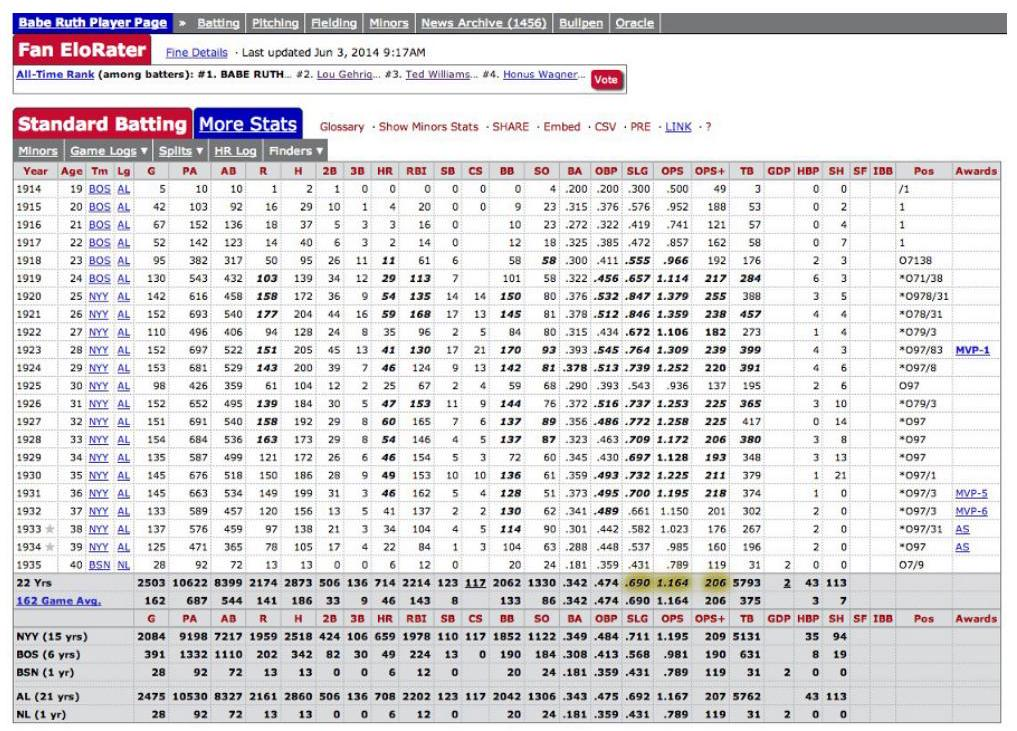
\includegraphics[max width=\textwidth]{2025_03_17_ca60ec0bfd96dcf8e028g-023}
    \caption{Statistical \textenglish{information} \textenglish{on} \textenglish{the} \textenglish{performance} \textenglish{of} \textenglish{Babe} \textenglish{Ruth} \textenglish{can} \textenglish{be} \textenglish{found} \textenglish{at} \href{http://www.baseball-reference.com}{http://www.baseball-reference.com}.}
    \label{fig:babe_ruth}
\end{figure}

कुंजी व्यापक रूप से सोचना है: बड़े, सामान्य प्रश्नों के उत्तर अक्सर अत्यधिक-विशिष्ट डेटा सैट्स में छिपे होते हैं, जिन्हें किसी भी तरह से उन्हें समाहित करने के लिए डिजाइन नहीं किया गया था।

\subsection{बेसबॉल इनसाइक्लोपीडिया}
\index{baseball encyclopedia}बेसबॉल का आँकड़ा विज्ञान की दुनिया में लंबे समय से एक विशेष महत्व रहा है। इस खेल को संयुक्त राज्य अमेरिका का राष्ट्रीय खेल कहा जाता है; वास्तव में, फ्रांसीसी इतिहासकार जाक बारज़ुन ने कहा कि "जो कोई भी अमेरिका के दिल और दिमाग को जानना चाहता है, उसे बेसबॉल सीखना चाहिए।" मैं समझता हूँ कि कई पाठक अमेरिकी नहीं हैं, और जो हैं भी, वे खेल में बिल्कुल रुचि नहीं रखते होंगे। लेकिन थोड़ी देर के लिए मेरे साथ बने रहें।\index{data!quantitative vs. categorical}\index{data!big vs. little}

क्या बेसबॉल को डेटा विज्ञान में महत्वपूर्ण बनाता है, वह है इसके खेल के व्यापक सांख्यिकीय रिकॉर्ड, जो सौ साल से भी अधिक समय से मौजूद हैं। बेसबॉल एक खेल है जिसमें अनेकों सीमित घटनाएँ होती हैं: पिचर्स गेंद फेंकते हैं और बल्लेबाज उन्हें मारने की कोशिश करते हैं - जो स्वाभाविक रूप से जानकारीपूर्ण सांख्यिकी की ओर ले जाता है। प्रशंसक बचपन में इन सांख्यांकों में डूब जाते हैं, जिससे वे मात्रात्मक विश्लेषण की शक्तियों और सीमाओं के बारे में अपनी समझ बनाते हैं। इनमें से कुछ बच्चे बड़े होकर डेटा वैज्ञानिक बन जाते हैं। वास्तव में, मूवी \textit{मनीबॉल}\index{Moneyball}में ब्रैड पिट की सांख्यिकी-समझ वाली बेसबॉल टीम की सफलता अमेरिकी जनता के लिए डेटा विज्ञान के साथ सबसे स्पष्ट संपर्क रहती है।

यह ऐतिहासिक बेसबॉल रिकॉर्ड \href{http://www.baseball-reference.com}{http://www.baseball-reference.com} पर उपलब्ध है। वहाँ आपको हर खिलाड़ी के प्रदर्शन के पूर्ण सांख्यिकीय डेटा मिलेंगे जिन्होंने मैदान पर कदम रखा था। इसमें प्रत्येक सत्र के बल्लेबाजी, पिचिंग और फील्डिंग रिकॉर्ड के सारांश आंकड़े शामिल हैं, साथ ही टीमों के बारे में जानकारी भी।

%---- \textenglish{Page} \textenglish{End} \textenglish{Break} \textenglish{Here} ---- \textenglish{Page} : 5

%--- \textenglish{Page} 5 ---

\begin{figure}[h]
    \centering
    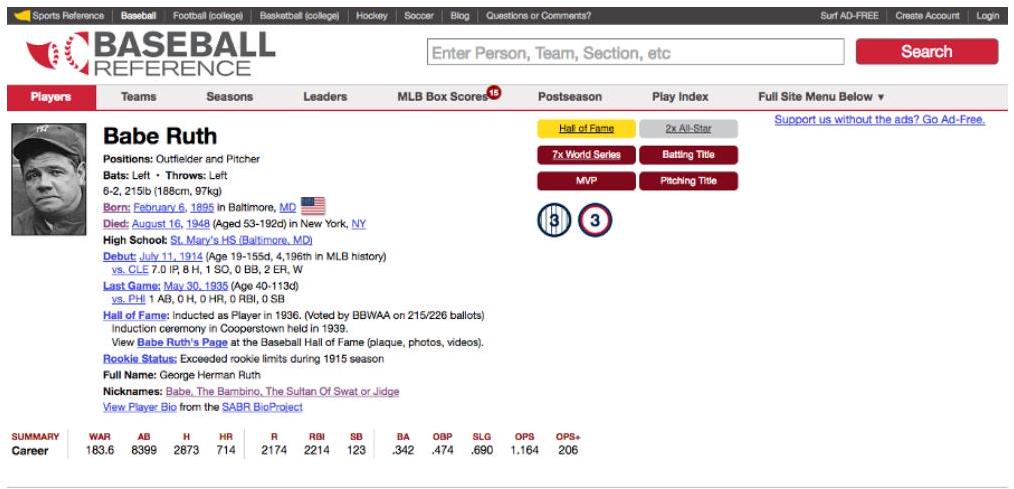
\includegraphics[max width=\textwidth]{2025_03_17_ca60ec0bfd96dcf8e028g-024}
    \caption{Personal \textenglish{information} \textenglish{on} \textenglish{every} \textenglish{major} \textenglish{league} \textenglish{baseball} \textenglish{player} \textenglish{is} \textenglish{available} \textenglish{at} \href{http://www.baseball-reference.com}{http://www.baseball-reference.com}.}
\end{figure}

लेकिन केवल सांख्यिकी से अधिक, सभी लोगों के जीवन और करियर के मेटाडेटा \index{metadata}जो कभी मेजर लीग बेसबॉल खेले हैं, जैसा कि चित्र 1.2 में दिखाया गया है। हम प्रत्येक खिलाड़ी के महत्वपूर्ण सांख्यिकी प्राप्त करते हैं (ऊंचाई, वजन, हाथ का प्रयोग) और उनकी जीवन अवधि (कब/कहाँ उनका जन्म हुआ और मृत्यु हुई)। हमें वेतन जानकारी भी मिलती है (प्रत्येक खिलाड़ी को हर मौसम में कितना वेतन मिला) और लेन-देन डेटा (वे कैसे बने प्रत्येक टीम के संपत्ति जिसके लिए उन्होंने खेला)।

अब, मुझे एहसास होता है कि आपमें से कई लोग बेसबॉल के बारे में थोड़ी सी भी जानकारी या रुचि नहीं रखते हैं। ⸨यह⸩ खेल कुछ हद तक ⸨क्रिकेट⸩ की याद दिलाता है, अगर यह मदद करता है। लेकिन याद रखें कि एक डेटा वैज्ञानिक के रूप में, आपके लिए यह आवश्यक है कि आप अपने आस-पास की दुनिया में रुचि लें। इसे कुछ नया सीखने के अवसर के रूप में देखें।

तो इस बेसबॉल डेटा सेट के साथ आप कौन से दिलचस्प प्रश्नों का उत्तर दे सकते हैं? आगे बढ़ने से पहले पाँच प्रश्न लिखने का प्रयास करें। चिंता न करें, मैं आपके खत्म करने का इंतजार करूंगा।

इस डेटा के साथ सबसे स्पष्ट प्रकार के प्रश्नों के उत्तर बेसबॉल से सीधे जुड़े होते हैं:

\begin{itemize}
  \item हम किसी व्यक्तिगत खिलाड़ी की कौशल या मूल्य का सबसे अच्छा मापन कैसे कर सकते हैं?\index{classification}\index{data \textenglish{science} television}\index{Quant Shop}
  \item आमतौर पर टीमों के बीच आदान-प्रदान कितना निष्पक्ष होता है?
  \item खिलाड़ी के प्रदर्शन स्तर की सामान्य प्रगति कैसी होती है जब वे परिपक्व और उम्रदराज होते हैं?
  \item बल्लेबाजी प्रदर्शन का खेली गई स्थिति के साथ कितना संबंध होता है? उदाहरण के लिए, क्या आउटफील्डर वास्तव में इनफील्डरों से बेहतर हिटर होते हैं?
\end{itemize}

ये दिलचस्प प्रश्न हैं। लेकिन इससे भी ज्यादा दिलचस्प हैं जनांकिकीय और सामाजिक मुद्दों के बारे में प्रश्न। लगभग 20,000 मुख्य लीग बेसबॉल खिलाड़ी-

%--- \textenglish{Page} 6 ---

पिछले 150 वर्षों में खिलाड़ियों ने मैदान में कदम रखा है, जिन्होंने पुरुषों के एक बड़े, व्यापक रूप से प्रलेखित समूह को प्रदान किया है जो बड़ी, कम प्रलेखित आबादी के लिए एक प्रॉक्सी के रूप में सेवा कर सकते हैं। वास्तव में, हम इस बेसबॉल खिलाड़ी डेटा का उपयोग करके ऐसे प्रश्नों का उत्तर दे सकते हैं जैसे:

\begin{itemize}
  \item क्या बाएँ हाथ के लोग दाएँ हाथ वालों की तुलना में कम जीवन जीते हैं? हैन्डेडनेस को अधिकतर जनसांख्यिकीय डेटा सेट्स में दर्ज नहीं किया गया है, लेकिन यहाँ इसे बड़े परिश्रम से इकट्ठा किया गया है। वास्तव में, इस डेटा सेट के विश्लेषण का उपयोग यह दिखाने के लिए किया गया है कि दाएँ हाथ वाले लोग बाएँ हाथ वालों की तुलना में लंबे समय तक जीवित रहते हैं [\cite{halpern1988right}]।
  \item लोग कितनी बार उसी जगह लौटते हैं जहाँ वे पैदा हुए थे? जन्म और मृत्यु के स्थानों को इस डेटा सेट में व्यापक रूप से दर्ज किया गया है। इसके अलावा, इनमें से लगभग सभी लोगों ने अपने करियर का कुछ हिस्सा घर से दूर खेला, इस प्रकार युवावस्था में महत्वपूर्ण समय पर उन्हें व्यापक दुनिया से परिचित कराया।
  \item क्या खिलाड़ियों की सैलरी सामान्यतः पिछले, वर्तमान, या भविष्य के प्रदर्शन को दर्शाती है?
  \item क्या समाज में ऊँचाई और वजन का अनुपात बढ़ा है?
\end{itemize}

यहाँ पर दो विशेष विषय हैं जिन पर ध्यान देना चाहिए। पहला, आइडेंटिफायर्स और रेफरेंस टैग्स (यानी मेटाडेटा) जो अक्सर डेटा सेट में उन चीजों से अधिक रोचक साबित होते हैं जिनकी हमें परवाह करनी चाहिए, यहाँ पर खेल का सांख्यिकीय रिकॉर्ड।

दूसरा विचार है a\textit{सांख्यिकीय प्रॉक्सी}, \index{statistical proxy} जहाँ आप उस डेटा सेट का उपयोग करते हैं जो आपके पास है, उस डेटा के स्थान पर जो आप वास्तव में चाहते हैं। आपके सपनों का डेटा सेट संभवतः अस्तित्व में नहीं है, या अगर है भी तो यह किसी कॉर्पोरेट दीवार के पीछे बंद हो सकता है। एक अच्छा डेटा वैज्ञानिक अभ्यासवादी होता है, जो यह देखता है कि वह जो कुछ उनके पास है उससे क्या कर सकते हैं, बजाय इसके कि वे जिस चीज़ तक नहीं पहुँच सकते उसकी शिकायत करें।

\subsection{इंटरनेट मूवी डेटाबेस (आईएमडीबी)}
\index{Internet \textenglish{Movie} Database}\index{IMDb}
हर कोई फिल्मों को पसंद करता है। इंटरनेट मूवी डेटाबेस (आईएमडीबी) में मोशन पिक्चर इंडस्ट्री के सभी पहलुओं के बारे में क्राउडसोर्स और क्यूरेटेड डेटा होता है, @ पर। आईएमडीबी में वर्तमान में 3.3 मिलियन से अधिक फिल्मों और टीवी कार्यक्रमों का डेटा शामिल है। प्रत्येक फिल्म के लिए, आईएमडीबी में इसका शीर्षक, चलने का समय, शैलियाँ, रिलीज़ की तारीख, और कास्ट और क्रू की पूरी सूची शामिल है। प्रत्येक उत्पादन के बारे में वित्तीय डेटा भी है, जिसमें फिल्म बनाने के लिए बजट और बॉक्स ऑफिस पर उसकी सफलता शामिल है।

अंत में, प्रत्येक फिल्म के लिए दर्शकों और समीक्षकों से विस्तृत रेटिंग्स उपलब्ध हैं। यह रेटिंग डेटा शून्य से दस सितारों के पैमाने पर अंक होते हैं, जिन्हें उम्र और लिंग के आधार पर औसत में सम्मिलित किया जाता है। लिखित समीक्षाएं अक्सर शामिल होती हैं, जो यह बताती हैं कि किसी विशेष आलोचक ने क्यों एक निश्चित संख्या में सितारे दिए। फिल्मों के बीच कड़ियाँ भी होती हैं: उदाहरण के लिए, यह पहचानना कि \textit{इट्स अ वंडरफुल लाइफ} के दर्शकों द्वारा कौन सी अन्य फिल्में सबसे अधिक देखी गई हैं।

हर अभिनेता, निर्देशक, निर्माता, और फिल्म से जुड़े क्रू सदस्य को आईएमडीबी में प्रविष्टि का हक़दार है, जिसमें अब 6.5 मिलियन लोगों का डेटा मौजूद है।

%---- \textenglish{Page} \textenglish{End} \textenglish{Break} \textenglish{Here} ---- \textenglish{Page} : 7

\clearpage
\label{sec:questions_data}

\begin{figure}
  \centering
  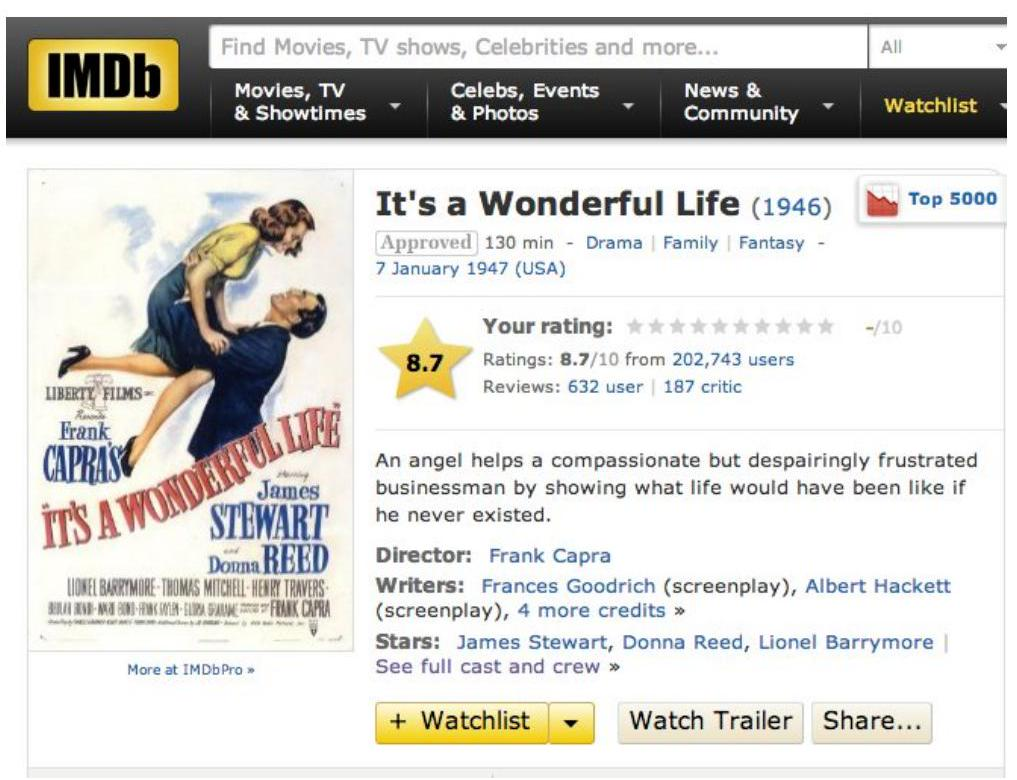
\includegraphics[max width=\textwidth]{2025_03_17_ca60ec0bfd96dcf8e028g-026}\index{General Sentiment}\index{natural \textenglish{language} processing}\index{Stony \textenglish{Brook} University}\index{Wikipedia}\index{genius}\index{wisdom}
  \caption{Representative \textenglish{film} \textenglish{data} \textenglish{from} \textenglish{the} \textenglish{Internet} \textenglish{Movie} Database.}
  \label{fig:imdb_film_data}
\end{figure}

\begin{figure}
  \centering
  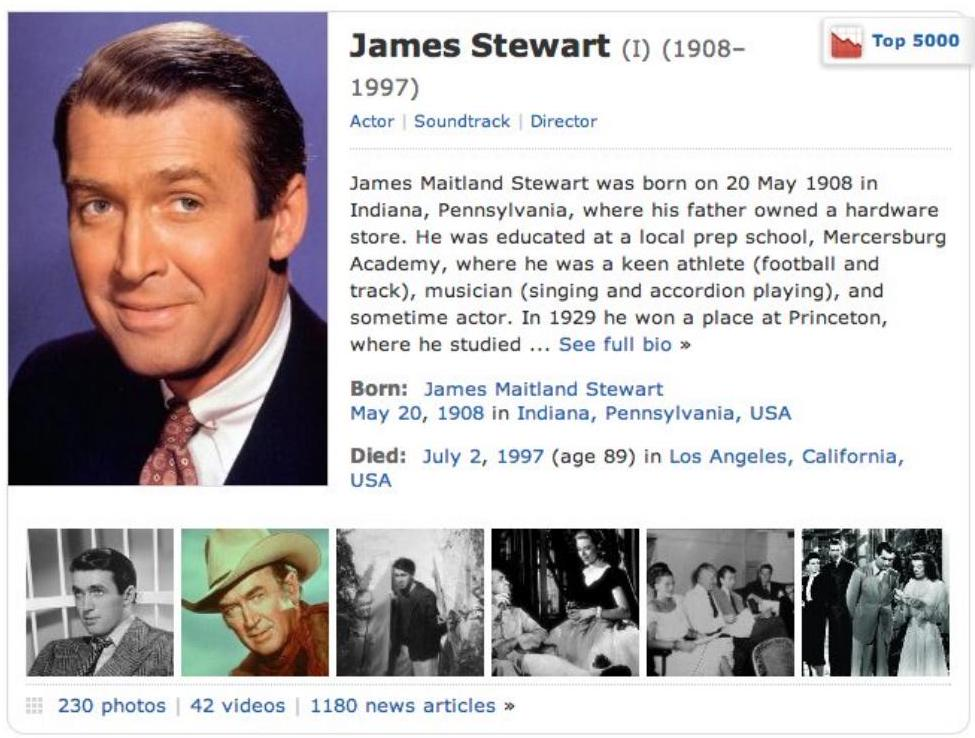
\includegraphics[max width=\textwidth]{2025_03_17_ca60ec0bfd96dcf8e028g-026(1)}
  \caption{Representative \textenglish{actor} \textenglish{data} \textenglish{from} \textenglish{the} \textenglish{Internet} \textenglish{Movie} Database.}
  \label{fig:imdb_actor_data}
\end{figure}

इनमें मेरे भाई, चचेरे भाई, और भाभी शामिल हैं। प्रत्येक अभिनेता को उनके द्वारा की गई हर फिल्म से जोड़ा गया है, उनके भूमिका के विवरण और क्रेडिट में उनकी स्थिति के साथ। प्रत्येक व्यक्तित्व के बारे में उपलब्ध डेटा में जन्म/मृत्यु तिथियाँ, ऊँचाई, पुरस्कार, और पारिवारिक संबंध शामिल हैं।

तो आप इस मूवी डाटा के साथ किस प्रकार के प्रश्नों का उत्तर दे सकते हैं?

शायद सबसे स्वाभाविक प्रश्न जो \textenglish{IMDb} से पूछे जा सकते हैं, वे फिल्मों और अभिनेताओं की चरम सीमाओं की पहचान से संबंधित होते हैं:

\begin{itemize}
  \item कौन से अभिनेता सबसे अधिक फिल्मों में दिखाई दिए? सबसे अधिक पैसा कमाया? सबसे कम रेटिंग वाली फिल्मों में दिखाई दिए? जिसका करियर सबसे लंबा था या जीवनकाल सबसे छोटा था?
  \item हर साल की सबसे उच्च रेटिंग वाली फिल्म कौन सी थी, या प्रत्येक विधा में सबसे अच्छी फिल्म कौन सी थी? कौन सी फिल्में सबसे अधिक पैसा खो गईं, सबसे शक्तिशाली कलाकारों की टुकड़ी थी, या सबसे कम अनुकूल समीक्षाएं प्राप्त हुईं?
\end{itemize}

फिर बड़े पैमाने पर सवाल उठाए जा सकते हैं जो स्वभाव में चलचित्र व्यवसाय के बारे में होते हैं:

\begin{itemize}
  \item क्या मूवी की कमाई दर्शकों की रेटिंग्स या पुरस्कारों के साथ कितना सम्बंधित है? क्या ग्राहक स्वाभाविक रूप से खराब फिल्मों की ओर आकर्षित होते हैं, या क्या रचनात्मक टीम की गुणवत्ता को सही रूप से पुरस्कृत किया जाता है?
  \item रेटिंग्स, बजट और कमाई के मामले में हॉलीवुड फिल्मों की तुलना बॉलीवुड फिल्मों से कैसे होती है? क्या अमेरिकी फिल्में विदेशी फिल्मों की तुलना में बेहतर तरीके से स्वीकार की जाती हैं, और यह अंतर यू.एस. और गैर-यू.एस. समीक्षकों के बीच कैसे भिन्न होता है?
  \item फिल्मों में अभिनेताओं और अभिनेत्रियों की आयु वितरण क्या है? पत्नी का किरदार निभा रही अभिनेत्री की उम्र, औसतन, पति का किरदार निभा रहे अभिनेता से कितनी कम होती है? क्या यह असमानता समय के साथ बढ़ रही है या घट रही है?
  \item तेजी से जियो, युवा मरो, और सुंदर शव छोड़ो? क्या मूवी सितारे साधारण जनता के मुकाबले, या छोटे किरदार निभाने वालों के मुकाबले लंबा या छोटा जीवन जीते हैं?
\end{itemize}

यह मानते हुए कि फिल्म पर काम करने वाले लोग एक-दूसरे को जानते हैं, कास्ट और क्रू डेटा का उपयोग फिल्म व्यवसाय का एक सामाजिक नेटवर्क बनाने के लिए किया जा सकता है। अभिनेताओं का सामाजिक नेटवर्क कैसा दिखता है? बेकन का ओरैकल\\index{Oracle \textenglish{of} Bacon}footnote{\url{https://oracleofbacon.org/}} केविन बेकन को हॉलीवुड ब्रह्मांड के केंद्र में रखता है और किसी भी अन्य अभिनेता से बेकन तक का सबसे छोटा रास्ता उत्पन्न करता है। सैमुअल एल. जैक्सन जैसे अन्य अभिनेता, और भी अधिक केंद्रीय साबित होते हैं।

और महत्वपूर्ण बात यह है कि क्या हम इस डेटा का विश्लेषण कर सकते हैं ताकि यह निर्धारित किया जा सके कि कोई व्यक्ति किसी विशेष फिल्म को पसंद करेगा या नहीं? \textit{सहयोगात्मक फ़िल्टरिंग} की तकनीक उन लोगों को ढूंढती है जिन्होंने उन फ़िल्मों को पसंद किया जो मैंने भी पसंद की, और उन फ़िल्मों की अनुशंसा करती है जो उन्हें अच्छी लगती थीं, जो मेरे लिए अच्छे उम्मीदवार हो सकते हैं। 2007 का नेटफ्लिक्स प्राइज \$1,000,000 की प्रतिस्पर्धा थी जिसका उद्देश्य एक रेटिंग इंजन बनाना था जो नेटफ्लिक्स की मालिकाना प्रणाली से 10\% बेहतर हो। इस पुरस्कार के अंतिम विजेता (\textenglish{BellKor}) ने विभिन्न डेटा स्रोतों और तकनीकों का उपयोग किया, जिसमें लिंक का विश्लेषण~\cite{bell2007lessons}.\index{sabermetrics} शामिल था।

\clearpage
\subsection{गूगल एनग्राम्स}\label{उप अनुभाग:गूगल_एनग्राम्स}

\begin{figure}
  \centering
  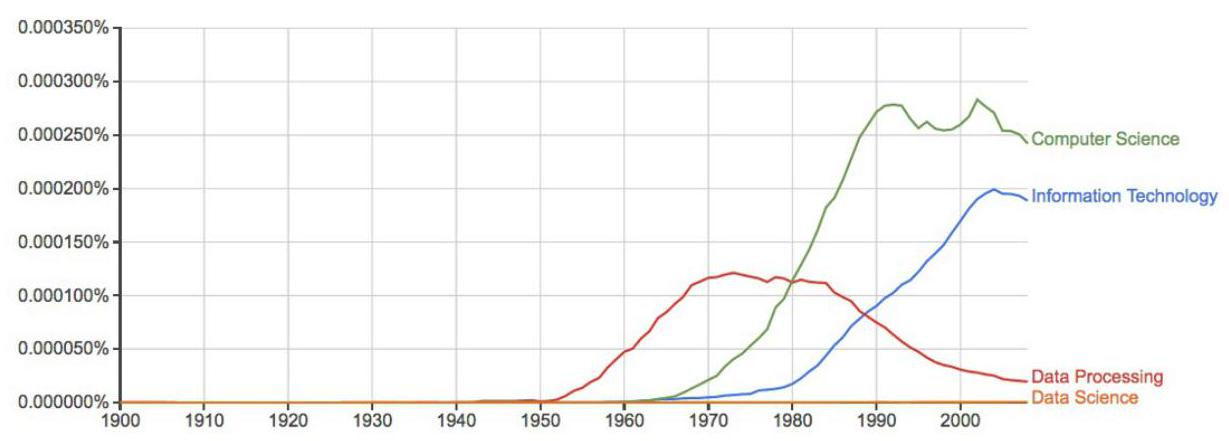
\includegraphics[max width=\textwidth]{2025_03_17_ca60ec0bfd96dcf8e028g-028}
  \caption{The \textenglish{rise} \textenglish{and} \textenglish{fall} \textenglish{of} \textenglish{data} processing, \textenglish{as} \textenglish{witnessed} \textenglish{by} \textenglish{Google} Ngrams.}
  \label{fig:google_ngrams}
\end{figure}

मुद्रित पुस्तकें मानव ज्ञान का मुख्य भंडार रही हैं, गुटेनबर्ग द्वारा 1439 में चल प्रकार के आविष्कार के बाद से। भौतिक वस्तुएं आज की डिजिटल दुनिया में कुछ हद तक असहज महसूस करती हैं, लेकिन प्रौद्योगिकी के पास सब कुछ डेटा में परिवर्तित करने की क्षमता होती है। दुनिया की जानकारी को संगठित करने के अपने मिशन के हिस्से के रूप में, गूगल ने दुनिया की सभी प्रकाशित पुस्तकों को स्कैन करने का प्रयास किया। वे अभी तक पूरी तरह से वहां नहीं पहुंचे हैं, लेकिन अब तक डिजिटाइज़ की गई 30 मिलियन पुस्तकें सभी प्रकाशित पुस्तकों का 20% से अधिक का प्रतिनिधित्व करती हैं।

गूगल इस डेटा का उपयोग खोज परिणामों को सुधारने और प्रिंट से बाहर की किताबों को नई पहुंच देने के लिए करता है। लेकिन शायद सबसे अच्छा उत्पाद है \textit{गूगल एनग्राम्स}, जो सांस्कृतिक काल की बदलावों का निरीक्षण करने के लिए एक अद्भुत संसाधन है। यह प्रत्येक वर्ष प्रकाशित किताबों में छोटी वाक्यांशों की आवृत्ति प्रदान करता है। प्रत्येक वाक्यांश को उनके स्कैन किए गए पुस्तक संकलन में कम से कम चालीस बार प्रकट होना चाहिए। यह अस्पष्ट शब्दों और वाक्यांशों को समाप्त कर देता है, लेकिन विश्लेषण के लिए दो अरब से अधिक समय श्रेणियाँ छोड़ देता है।

यह समृद्ध डेटा सेट दिखाता है कि पिछले 200 वर्षों में भाषा का उपयोग कैसे बदल गया है, और इसे सांस्कृतिक प्रवृत्ति विश्लेषण में व्यापक रूप से लागू किया गया है~\cite{MAV+11}। चित्र~\ref{fig:google_ngrams}इस डेटा का उपयोग यह दिखाने के लिए करता है कि \textit{data} शब्द कंप्यूटिंग के बारे में सोचते समय कैसे अपनी लोकप्रियता खो बैठा। 1950 के दशक के पंच कार्ड और घूमते हुए चुंबकीय टेप के युग में कंप्यूटिंग क्षेत्र से संबंधित लोकप्रिय शब्द \textit{Data processing} था। \textenglish{Ngrams} डेटा दिखाता है कि \textit{Computer Science} के तेजी से उभार ने 1980 तक \textit{Data Processing} को नहीं पछाड़ा। आज भी, \textit{Data Science} इस पैमाने पर लगभग अदृश्य रहता है।

गूगल एनग्राम्स को\url{http://books.google.com/ngrams}पर देखें। मैं वादा करता हूँ कि आप इसके साथ खेलकर आनंद लेंगे। तुलना करें\textit{हॉट डॉग}को\textit{टोफू}से,\textit{विज्ञान}को\textit{धर्म}के साथ,\textit{स्वतंत्रता}को\textit{न्याय}से, और\textit{सेक्स}को\textit{विवाह}से, इस अद्भुत दूरबीन से अतीत को समझने के लिए। 

लेकिन एक बार जब आप खेलना समाप्त कर लें, तो उन बड़ी चीजों के बारे में सोचें जो आप कर सकते थे अगर आपके पास इस डेटा तक पहुंच होती। मान लें कि आपके पास पिछले 200 वर्षों में पुस्तकों में प्रकाशित \textit{सभी} शब्दों/वाक्यांशों के वार्षिक संदर्भों की संख्या तक पहुंच है।

%---- \textenglish{Page} \textenglish{End} \textenglish{Break} \textenglish{Here} ---- \textenglish{Page} : 10



गूगल इस डेटा को मुफ्त में उपलब्ध कराता है। तो आप इसके साथ क्या करने वाले हैं?

एनग्राम्स व्यूअर का उपयोग करके विशेष शब्दों से संबंधित समय श्रृंखला का निरीक्षण करना मजेदार है। लेकिन अधिक परिष्कृत ऐतिहासिक रुझानों को एकाधिक समय श्रृंखलाओं को एक साथ जोड़कर पकड़ा जा सकता है। मुझे निम्न प्रकार के प्रश्न विशेष रूप से दिलचस्प लगते हैं:

\begin{itemize}
  \item समय के साथ गाली देने की मात्रा कैसे बदल गई है? जिन चार-अक्षरों वाले शब्दों से मैं सबसे ज्यादा परिचित हूँ, उनका उपयोग 1960 के बाद से बहुत ज्यादा बढ़ गया लगता है, हालांकि यह कम स्पष्ट है कि यह गाली-गलौज में वृद्धि को दर्शाता है या प्रकाशन मानकों में गिरावट को।
  \item नई शब्दावली कितनी बार उभरती है और लोकप्रिय होती है? क्या ये शब्द आम उपयोग में रहते हैं, या तेजी से गायब हो जाते हैं? क्या हम यह पता लगा सकते हैं कि समय के साथ शब्दों का अर्थ कैसे बदलता है, जैसे \textit{gay} का \textit{happy} से \textit{homosexual} में परिवर्तन? 
  \item क्या शब्दों की वर्तनी के मानक समय के साथ सुधर रहे हैं या बिगड़ रहे हैं, खासकर अब जब हम स्वचालित वर्तनी जांच के युग में प्रवेश कर चुके हैं? विरले-घटने वाले शब्द जो एक सामान्य उपयोग वाले शब्द से केवल एक अक्षर से भिन्न हैं, वर्तनी त्रुटियों के संभावित उम्मीदवार हो सकते हैं (जैसे \textit{algorithm} बनाम \textit{algorthm})। कई अलग-अलग गलत वर्तनी के ऊपर मिलाकर, क्या ऐसी त्रुटियाँ बढ़ रही हैं या घट रही हैं?
\end{itemize}

आप इस एनग्राम्स कोरपस का उपयोग एक भाषा मॉडल बनाने के लिए कर सकते हैं जो किसी दी गई भाषा में शब्दों के अर्थ और उपयोग को पकड़ता है। हम खंड 11.6.3 में शब्द एम्बेडिंग्स पर चर्चा करेंगे, जो भाषा मॉडल बनाने के लिए शक्तिशाली उपकरण हैं। आवृत्ति गणना यह प्रकट करती है कि कौन से शब्द सबसे लोकप्रिय हैं। शब्द युग्मों की आवृत्ति, जो एक-दूसरे के पास दिखाई देती हैं, श्रवण पहचान प्रणालियों को सुधारने के लिए उपयोग की जा सकती हैं, जिससे यह पता लगाने में मदद मिलती है कि वक्ता ने \textit{that's \textenglish{too} bad} कहा या \textit{that's \textenglish{to} bad}। ये लाखों पुस्तकें प्रतिनिधि मॉडल बनाने के लिए पर्याप्त डेटा सेट प्रदान करती हैं।

\subsection{न्यू यॉर्क टैक्सी रिकॉर्ड्स}

आजकल हर वित्तीय लेन-देन अपने पीछे डेटा का निशान छोड़ता है। इन रास्तों का अनुसरण करके दिलचस्प अंतर्दृष्टियाँ प्राप्त की जा सकती हैं।

टैक्सी कैब्स शहरी परिवहन नेटवर्क का एक महत्वपूर्ण हिस्सा हैं। वे शहर की सड़कों पर ग्राहकों की तलाश में घूमते हैं, और फिर उन्हें यात्रा की लंबाई के अनुपात में किराए के लिए उनके गंतव्य तक पहुंचाते हैं। प्रत्येक कैब में एक मीटरिंग डिवाइस होती है जो यात्रा की लागत को समय के अनुसार गणना करती है। यह मीटर एक रिकॉर्ड रखने का उपकरण है, और यह सुनिश्चित करने का तंत्र है कि चालक प्रत्येक यात्रा के लिए उचित राशि चार्ज करे।

न्यूयॉर्क की टैक्सियों में वर्तमान में उपयोग किए जा रहे टैक्सी मीटर किराया गिनने से कहीं अधिक काम कर सकते हैं। ये क्रेडिट कार्ड टर्मिनल की तरह काम करते हैं, जो एक तरीका प्रदान करते हैं

\begin{figure}[h]
\centering
\begin{tabular}{|c|c|c|c|c|c|c|c|c|c|}
\hline
\textenglish{Vendor} \textenglish{ID} & \textenglish{passenger} \textenglish{count} & \textenglish{trip} \textenglish{distance} & \textenglish{pickup} \textenglish{longitude} & \begin{tabular}{l}
pickup\_ \\
\textenglish{latitude} \\
\end{tabular} & \textenglish{dropoff} \textenglish{longitude} & dropoff\_ & \textenglish{payment} \textenglish{type} & \( \begin{aligned} & \text { tip_- } \\ & \text { \textenglish{amount} } \end{aligned} \) & \textenglish{total} \textenglish{amount} \\
\hline
2 & 1 & 7.22 & -73.9998 & 40.74334 & -73.9428 & 40.80662 & 2 & 0 & 30.8 \\
\hline
1 & 1 & 2.3 & -73.977 & 40.7749 & -73.9783 & 40.74986 & 1 & 2.93 & 16.23 \\
\hline
1 & 1 & 1.5 & -73.9591 & 40.77513 & -73.9804 & 40.78231 & 1 & 1.65 & 9.95 \\
\hline
1 & 1 & 0.9 & -73.9766 & 40.78075 & -73.9706 & 40.78885 & 1 & 1.45 & 8.75 \\
\hline
2 & 1 & 2.44 & -73.9786 & 40.78592 & -73.9974 & 40.7563 & 1 & 2 & 16.3 \\
\hline
2 & 1 & 3.36 & -73.9764 & 40.78589 & -73.9424 & 40.82209 & 1 & 3.58 & 17.88 \\
\hline
2 & 2 & 2.34 & -73.9862 & 40.76087 & -73.9569 & 40.77156 & 1 & 1 & 13.8 \\
\hline
2 & 1 & 10.19 & -73.79 & 40.64406 & -73.9312 & 40.67588 & 2 & 0 & 32.8 \\
\hline
1 & 2 & 3.3 & -73.9937 & 40.72738 & -73.9982 & 40.7641 & 1 & 2 & 21.3 \\
\hline
1 & 1 & 1.8 & -73.9949 & 40.74006 & -73.9767 & 40.74934 & 1 & 1.85 & 11.15 \\
\hline
\end{tabular}
\caption{Representative \textenglish{fields} \textenglish{from} \textenglish{the} \textenglish{New} \textenglish{York} \textenglish{city} \textenglish{taxi} \textenglish{cab} data: \textenglish{pick} \textenglish{up} \textenglish{and} \textenglish{dropoff} points, distances, \textenglish{and} fares.}
\end{figure}

ग्राहकों के लिए नकद के बिना सवारी का भुगतान करने के लिए। वे ग्लोबल पोजिशनिंग सिस्टम्स\index{Global \textenglish{Positioning} System} (\textenglish{GPS}) के साथ एकीकृत हैं, जो हर पिकअप और ड्रॉप ऑफ का सटीक स्थान रिकॉर्ड करते हैं। और अंत में, क्योंकि वे एक वायरलेस नेटवर्क पर हैं, ये बॉक्स इस सभी डेटा को एक केंद्रीय सर्वर पर वापस भेज सकते हैं।

परिणाम एक डेटाबेस है जो दुनिया के सबसे महान शहरों में से एक के सभी टैक्सी कैब द्वारा की गई हर एक यात्रा का दस्तावेजीकरण करता है, जिसका एक छोटा सा हिस्सा चित्र 1.6 में दिखाया गया है। क्योंकि न्यूयॉर्क टैक्सी और लिमोसिन कमिशन एक सार्वजनिक एजेंसी है, इसकी गैर-गोपनीय डेटा सभी के लिए सूचना की स्वतंत्रता अधिनियम (\textenglish{FOA}) के तहत उपलब्ध है।

हर सवारी दो रिकॉर्ड उत्पन्न करती है: एक यात्रा के डेटा के साथ, दूसरा किराए के विवरण के साथ। हर यात्रा को प्रत्येक कार के मैडलियन (लाइसेंस) और प्रत्येक चालक के पहचानकर्ता के साथ जोड़ा जाता है। प्रत्येक यात्रा के लिए, हमें पिकअप और ड्रॉप-ऑफ का समय/तारीख मिलती है, साथ ही शुरुआती स्थान और गंतव्य के जीपीएस स्थानांको (लॉन्गिट्यूड और लैटीट्यूड) मिलते हैं। हमें उन बिंदुओं के बीच यात्रा किए गए मार्ग के जीपीएस डेटा नहीं मिलते, लेकिन कुछ हद तक इसे उनके बीच के सबसे छोटे रास्ते द्वारा अनुमानित किया जा सकता है।

किराया डेटा के लिए, हमें प्रत्येक यात्रा की मीटर की गई लागत मिलती है, जिसमें कर, अधिभार और टोल शामिल हैं। सेवा के लिए ड्राइवर को टिप देना पारंपरिक है, जिसकी राशि भी डेटा में दर्ज की जाती है।

तो मैं तुमसे बात कर रहा हूँ। यह टैक्सी डेटा आसानी से उपलब्ध है, जिसमें पिछले कई वर्षों में 80 मिलियन से अधिक यात्राओं के रिकॉर्ड हैं। तुम इसके साथ क्या करने वाले हो?

कोई भी रोचक डेटा सेट विभिन्न पैमानों पर प्रश्नों का उत्तर देने के लिए उपयोग किया जा सकता है। यह टैक्सी किराया डेटा हमें परिवहन उद्योग को बेहतर तरीके से समझने में मदद कर सकता है, लेकिन साथ ही यह समझने में भी कि शहर कैसे काम करता है और हम इसे और भी बेहतर कैसे बना सकते हैं। टैक्सी उद्योग के संदर्भ में प्राकृतिक प्रश्नों में शामिल हैं:

%---- \textenglish{Page} \textenglish{End} \textenglish{Break} \textenglish{Here} ---- \textenglish{Page} : 12



\label{अनुभाग:प्रश्न पूछना}

\begin{figure}[h]
    \centering
    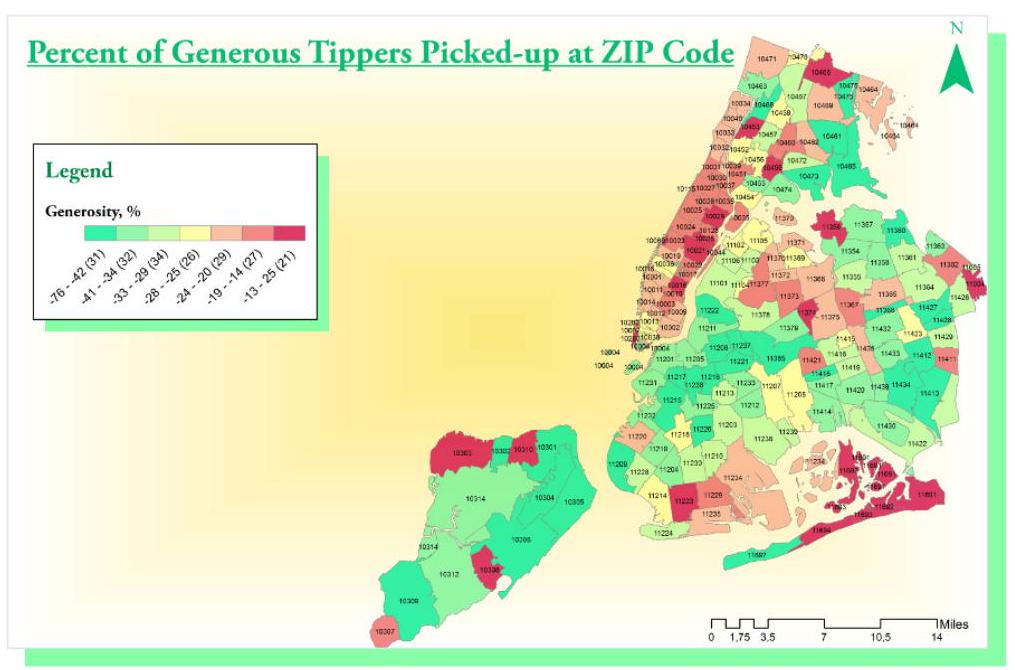
\includegraphics[max width=\textwidth]{2025_03_17_ca60ec0bfd96dcf8e028g-031}
    \caption{Which \textenglish{neighborhoods} \textenglish{in} \textenglish{New} \textenglish{York} \textenglish{City} \textenglish{tip} \textenglish{most} generously? \textenglish{The} \textenglish{relatively} \textenglish{remote} \textenglish{outer} \textenglish{boroughs} \textenglish{of} \textenglish{Brooklyn} \textenglish{and} Queens, \textenglish{where} \textenglish{trips} \textenglish{are} \textenglish{longest} \textenglish{and} \textenglish{supply} \textenglish{is} \textenglish{relatively} scarce.}\index{conditional probability}\index{Fermat, \textenglish{Pierre} de}\index{independence}\index{Pascal, Blaise}\index{conditional probability}
    \label{fig:nyc_neighborhoods}
\end{figure}

\begin{itemize}
  \item ड्राइवर रात में औसतन कितने पैसे कमाते हैं? वितरण कैसा है? क्या ड्राइवर धूप वाले दिनों में अधिक कमाते हैं या बारिश वाले दिनों में?
  \item शहर के कौन-कौन से स्थान ड्राइवरों के लिए सबसे अच्छे हैं जहाँ लाभदायक भाड़े उठाए जा सकें? यह दिन के अलग-अलग समय में कैसे बदलता है?
  \item ड्राइवर रात की शिफ्ट के दौरान कितनी दूरी तय करते हैं? हम इस डेटा सेट का उपयोग करके इसका सटीक उत्तर नहीं दे सकते हैं, क्योंकि इसमें किरायों के बीच यात्रा किए गए मार्ग की जीपीएस जानकारी नहीं है। लेकिन हमें अंतिम ड्रॉप-ऑफ स्थान, अगला पिक-अप स्थान, और उनके बीच पहुंचने में कितना समय लगा, यह पता है। यह एक उचित अनुमान लगाने के लिए पर्याप्त जानकारी प्रदान करना चाहिए।
  \item कौन से ड्राइवर अपने अनजान बाहरी क्षेत्र के यात्रियों को अधिक चार्ज करते हैं, जो कि छोटी, सस्ती यात्रा होनी चाहिए?
  \item ड्राइवर को कितनी टिप मिलती है, और क्यों? क्या तेजी से चलने वाले ड्राइवरों को बेहतर टिप मिलती है? टिलिंग की दरें क्षेत्र के हिसाब से कैसे बदलती हैं, और क्या यह अमीर इलाके हैं या गरीब इलाके जो अधिक उदार साबित होते हैं? मैं यह स्वीकार करता हूँ कि हमने इसका विश्लेषण किया है, जिसे मैं खंड~\ref{sec:war_story_taxi_deriver} में युद्ध कहानी में आगे वर्णन करूंगा। हमने कई दिलचस्प पैटर्न पाए \cite{starov2015gis}। आकृति~\ref{fig:nyc_neighborhoods} यह दिखाती है कि मैनहट्टनवासी आम तौर पर ब्रुकलीन, क्वीन और स्टेटन आइलैंड के बड़े क्षेत्र की अपेक्षा कंजूस होते हैं, जहाँ यात्राएँ लंबी होती हैं और स्ट्रीट टैक्सियाँ एक दुर्लभ लेकिन स्वागत योग्य दृश्य होती हैं।
\end{itemize}

लेकिन बड़े सवाल शहर में परिवहन को समझने से जुड़े हैं। हम टैक्सी यात्रा के समय को एक संवेदक के रूप में उपयोग करके शहर में यातायात के स्तर को बारीकी से माप सकते हैं। ⸨लोगों⸩ के आवागमन के समय यातायात अन्य समय की तुलना में कितना धीरे चलता है, और देरी सबसे अधिक कहां होती है? समस्या क्षेत्रों की पहचान करना समाधान प्रस्तावित करने का पहला कदम है, जैसे कि ट्रैफिक लाइट के समय के पैटर्न को बदलना, अधिक बसें चलाना, या केवल उच्च-आक्यूपेंसी के लिए लेन बनाना।

उसी प्रकार, हम टैक्सी डेटा का उपयोग कर सकते हैं ताकि पूरे शहर में परिवहन प्रवाह को मापा जा सके। लोग दिन के अलग-अलग समयों पर कहाँ यात्रा कर रहे हैं? यह हमें केवल भीड़भाड़ से कहीं अधिक बताता है। टैक्सी डेटा को देखकर, हम यह देख सकते हैं कि पर्यटक होटलों से आकर्षण स्थलों तक जा रहे हैं, उच्चस्थ अधिकारी शानदार मोहल्लों से वॉल स्ट्रीट तक जा रहे हैं, और नाइटक्लब में मस्ती के बाद नशे में धुत लोग घर लौट रहे हैं।

ऐसा डेटा बेहतर परिवहन प्रणालियों को डिजाइन करने के लिए आवश्यक है। यह फिजूलखर्ची है जब एक अकेला यात्री बिंदु$a$से बिंदु$b$तक यात्रा करता है, जबकि बिंदु$a+\epsilon$पर दूसरा यात्री भी वहाँ जाना चाहता है। टैक्सी डेटा का विश्लेषण एक राइड-शेयरिंग सिस्टम का सटीक सिमुलेशन करने में सक्षम बनाता है, ताकि हम ऐसी सेवा की मांग और लागत में कमी को सही से आकलित कर सकें।

\section{डेटा के गुण}
\index{data!properties}
यह पुस्तक डेटा का विश्लेषण करने की तकनीकों के बारे में है। लेकिन वह मूलभूत वस्तु क्या है जिसकी हम अध्ययन करेंगे? यह खंड डेटा के गुणों के एक संक्षिप्त वर्गीकरण प्रदान करता है, ताकि हम बेहतर ढंग से समझ सकें और सराह सकें कि हम किस पर काम कर रहे होंगे।

\subsection{संरचित बनाम असंरचित डेटा}
\index{data!unstructured}\index{data!structured}
कुछ डेटा सेट बहुत अच्छे से संगठित होते हैं, जैसे डेटाबेस या स्प्रेडशीट प्रोग्राम में तालिकाएँ। अन्य जानकारी विश्व की स्थिति के बारे में रिकॉर्ड करते हैं, लेकिन अधिक विषम तरीके से। शायद यह विकिपीडिया जैसे चित्रों और लिंक के साथ एक बड़ा टेक्स्ट संग्रह है, या व्यक्तिगत चिकित्सा रिकॉर्ड में दिखाई देने वाले नोट्स और परीक्षण परिणामों का जटिल मिश्रण है।

आम तौर पर, यह पुस्तक संरचित डेटा से निपटने पर केंद्रित होगी। डेटा को अक्सर एक \textit{मैट्रिक्स} द्वारा दर्शाया जाता है,\index{matrix} जहाँ मैट्रिक्स की पंक्तियाँ विशिष्ट वस्तुओं या अभिलेखों को दर्शाती हैं, और स्तंभ इन वस्तुओं की विशिष्ट विशेषताओं को दर्शाते हैं। उदाहरण के लिए, अमेरिकी शहरों के बारे में डेटा सेट में प्रत्येक शहर के लिए एक पंक्ति हो सकती है, जिसमें स्तंभ राज्य, जनसंख्या और क्षेत्र जैसी विशेषताओं को दर्शाते हैं।

जब हम एक असंरचित डेटा स्रोत का सामना करते हैं, जैसे कि ट्विटर से ट्वीट्स का संग्रह, तो हमारा पहला कदम आमतौर पर इसे संरचित करने के लिए एक मैट्रिक्स बनाना होता है। \textit{शब्दों का बस्ता} मॉडल एक मैट्रिक्स का निर्माण करेगा जिसमें प्रत्येक ट्वीट के लिए एक पंक्ति और प्रत्येक बार-बार उपयोग होने वाले शब्दावली शब्द के लिए एक स्तंभ होगा। मैट्रिक्स प्रविष्टि $M[i, j]$ तब यह दर्शाती है कि ट्वीट $i$ में शब्द $j$ कितनी बार शामिल है। ऐसे मैट्रिक्स संप्रेषण हमारे \ref{रेखीय बीजगणित} का अध्याय ~⸨chap:linear_algebra⸩ में चर्चा के लिए प्रेरित करेंगे।

%---- \textenglish{Page} \textenglish{End} \textenglish{Break} \textenglish{Here} ---- \textenglish{Page} : 14
\subsection{Quantitative vs. \textenglish{Categorical} Data}
\textit{Quantitative data} \textenglish{consists} \textenglish{of} \textenglish{numerical} values, \textenglish{like} \textenglish{height} \textenglish{and} weight. \textenglish{Such} \textenglish{data} \textenglish{can} \textenglish{be} \textenglish{incorporated} \textenglish{directly} \textenglish{into} \textenglish{algebraic} \textenglish{formulas} \textenglish{and} \textenglish{mathematical} models, \textenglish{or} \textenglish{displayed} \textenglish{in} \textenglish{conventional} \textenglish{graphs} \textenglish{and} charts.

इसके विपरीत, \textit{श्रेणीबद्ध डेटा} जाँच के अंतर्गत वस्तुओं के गुणों का वर्णन करने वाले लेबल होते हैं, जैसे लिंग, बालों का रंग, और व्यवसाय। यह वर्णनात्मक जानकारी उतनी ही सटीक और अर्थपूर्ण हो सकती है जितनी संख्यात्मक डेटा, लेकिन इसे उन्हीं तरीकों से नहीं निपटाया जा सकता।

श्रेणीबद्ध डेटा को सामान्यतः संख्यात्मक रूप में कोडित किया जा सकता है। उदाहरण के लिए, लिंग को\textit{male}$=0$या\textit{female}$=1$के रूप में प्रदर्शित किया जा सकता है। लेकिन जब किसी विशेषता के लिए दो से अधिक चर होते हैं, तो स्थिति और जटिल हो जाती है, विशेषकर जब उनमें कोई अंतर्निहित क्रम नहीं होता। हम विभिन्न हेयर रंगों को संख्याओं द्वारा कोडित कर सकते हैं, जैसे कि ग्रे हेयर$=0$, रेड हेयर$=1$, और ब्लॉन्ड हेयर$=2$का विशिष्ट मान प्रदान करके। तथापि, हम इन मूल्यों को अन्य किसी के लिए संख्याओं के रूप में बिल्कुल नहीं देख सकते, सिवाय साधारण पहचान परीक्षण के। क्या अधिकतम या न्यूनतम हेयर रंग के बारे में बात करना कोई समझ रखता है? आपके हेयर रंग से मेरे हेयर रंग को घटाने का क्या अर्थ है?

अधिकांश जो हम इस पुस्तक में करेंगे वह संख्यात्मक डेटा के इर्द-गिर्द ही होगा। लेकिन श्रेणीबद्ध विशेषताओं और उनके लिए काम करने वाली विधियों पर ध्यान बनाए रखें। श्रेणीबद्ध लेबल्स को संख्यात्मक डेटा से उत्पन्न करने वाली विधियाँ जैसे की क्लासिफिकेशन और क्लस्टरिंग विधियाँ, इस पुस्तक में मुख्य फोकस रहेंगी।

\subsection{बिग डेटा बनाम लिटिल डेटा}
डेटा साइंस को सार्वजनिक दृष्टि में \textit{बिग डेटा} के साथ मिलाकर देखा जा रहा है, जो कंप्यूटर लॉग्स और सेंसर डिवाइसों से उत्पन्न विशाल आंकड़ा सेटों का विश्लेषण है। सिद्धांत रूप से, अधिक डेटा होना हमेशा कम डेटा होने से बेहतर होता है, क्योंकि आप हमेशा सैंपलिंग द्वारा इसे छोटा करने के लिए कुछ डेटा को फेंक सकते हैं यदि आवश्यक हो।

बिग डेटा एक रोमांचक घटना है, और हम इसे अध्याय 12 में चर्चा करेंगे। लेकिन व्यवहार में, बड़े डेटा सेट के साथ काम करने में कठिनाइयाँ होती हैं। इस पुस्तक में हम डेटा के विश्लेषण के लिए एल्गोरिदम और सर्वोत्तम प्रथाओं पर विचार करेंगे। सामान्य रूप से, चीजें तब कठिन हो जाती हैं जब वॉल्यूम बहुत बड़ा हो जाता है। बिग डेटा की चुनौतियों में शामिल हैं:

\begin{itemize}\index{signal \textenglish{to} \textenglish{noise} ratio}\index{stock market}\index{variance!interpretation}
\item \textit{जैसे-जैसे डेटा का आकार बढ़ता है, विश्लेषण चक्र समय धीमा हो जाता है}: डेटा सेट्स पर गणनात्मक ऑपरेशन्स जितना अधिक होता है, उतनी ही अधिक देर लगती है। छोटे स्प्रेडशीट्स तत्क्षण प्रतिक्रिया देते हैं, जिससे आपको परीक्षण और \textit{अगर ऐसा होता तो}? खेलने की सुविधा मिलती है। लेकिन बड़े स्प्रेडशीट्स के साथ काम करना धीमा और बोझिल हो सकता है, और बहुत बड़े डेटा सेट्स से उत्तर प्राप्त करने में घंटों या दिनों का समय लग सकता है।
\item \textit{बड़े डेटा सेट्स को विज़ुअलाइज़ करना जटिल होता है}: इनमें लाखों पॉइंट्स के साथ प्लॉट्स को कंप्यूटर स्क्रीन या मुद्रित छवियों पर प्रदर्शित करना असंभव है, और इसे विचारशील रूप से समझना तो दूर की बात है। हम किसी ऐसी चीज़ को वास्तव में कैसे समझ सकते हैं जिसे हम देख नहीं सकते?
\item \textit{सरल मॉडल्स को फिट या मूल्यांकन करने के लिए विशाल डेटा की आवश्यकता नहीं होती}: एक सामान्य डेटा साइंस कार्य का उदाहरण निर्णय लेना हो सकता है (जैसे, क्या मुझे इस व्यक्ति को जीवन बीमा देना चाहिए?) कुछ संख्या में वेरिएबल्स के आधार पर: जैसे आयु, लिंग, ऊँचाई, वजन, और मौजूदा चिकित्सकीय स्थितियों की उपस्थिति या अनुपस्थिति।
\end{itemize}

यदि मेरे पास 10 लाख लोगों के बारे में डेटा है जिसमें उनके संबंधित जीवन परिणाम शामिल हैं, तो मुझे कवरेज जोखिम का एक अच्छा सामान्य मॉडल बनाने में सक्षम होना चाहिए। अगर मेरे पास यह डेटा करोड़ों लोगों पर होता, तो यह शायद मुझे काफी बेहतर मॉडल बनाने में मदद नहीं करता। केवल कुछ वेरिएबल्स (जैसे आयु और वैवाहिक स्थिति) के आधार पर निर्णय मानदंड बहुत जटिल नहीं हो सकते हैं और इसे बड़ी संख्या में आवेदकों पर मजबूत होना चाहिए। कोई भी निरीक्षण जो इतना सूक्ष्म हो कि उसे निकालने के लिए विशाल डेटा की आवश्यकता हो, उसे उस बड़े व्यवसाय के लिए अप्रासंगिक साबित होगा जो बड़ी मात्रा पर आधारित है।

\textit{बिग डेटा}को कभी-कभी \textit{बैड डेटा}कहा जाता है। यह अक्सर किसी दिए गए सिस्टम या प्रक्रिया का उप-उत्पाद के रूप में इकट्ठा किया जाता है, बजाय इसके कि इसे आपके प्रश्न का उत्तर देने के लिए उद्देश्यपूर्ण रूप से संग्रहित किया जाए। परिणामस्वरूप, हमें किसी चीज़ को समझने के लिए साहसिक प्रयास करने पड़ सकते हैं, केवल इसलिए कि हमारे पास यह है।

राष्ट्रपति उम्मीदवारों के बीच मतदाता प्राथमिकताओं पर विचार करने की समस्या पर विचार करें। बिग डेटा दृष्टिकोण बड़े पैमाने पर ट्विटर या फेसबुक फीड्स का विश्लेषण कर सकता है, जो उनकी राय के सुराग को पाठ में व्याख्यायित करता है। स्मॉल डेटा दृष्टिकोण हो सकता है कि एक सर्वेक्षण किया जाए, जिसमें कुछ सैकड़ों लोगों से यह विशिष्ट प्रश्न पूछा जाए और परिणामों को संकलित किया जाए। आपको कौन सी प्रक्रिया अधिक सटीक लगेगी? सही डेटा सेट वह है जो हाथ में दिए गए कार्य से सबसे अधिक सीधे रूप में संबंधित है, न कि जरूरी रूप से सबसे बड़ा।

\textit{घर पर सीखने का पाठ}: बिना सोचे-समझे बड़े डेटा सेट्स का विश्लेषण करने की आकांक्षा न करें। किसी दिए गए प्रश्न का उत्तर देने के लिए \textit{सही} डेटा की तलाश करें, जरूरी नहीं कि जो सबसे बड़ा हो वह आपके हाथ लग जाए।

\section{वर्गीकरण और प्रतिगमन}
\index{regression}परंपरागत डेटा विज्ञान और पैटर्न पहचान अनुप्रयोगों में दो प्रकार की समस्याएँ बार-बार उत्पन्न होती हैं, जो हैं वर्गीकरण और प्रतिगमन की चुनौतियाँ। जैसे-जैसे इस पुस्तक का विकास हुआ है, मैंने इन समस्याओं को हल करने के लिए एल्गोरिदमिक दृष्टिकोणों की चर्चाओं को बाद के अध्यायों की ओर धकेला है, ताकि वे डेटा मंगिंग, सांख्यिकी, दृश्यात्मकता, और गणितीय मॉडलिंग के मूलभूत सामग्री की ठोस समझ से लाभान्वित हो सकें।\index{characterizing distributions}\index{performance \textenglish{of} models}

फिर भी, मैं वर्गीकरण और प्रत्यास्थता से संबंधित मुद्दों का उल्लेख करूँगा जैसे ही वे उत्पन्न होते हैं, इसलिए इन समस्याओं की एक त्वरित परिचय के लिए यहाँ ठहरना समझदारी होगी, ताकि आप उन्हें पहचान सकें जब आप इन्हें देखें।



% \textenglish{Continue} \textenglish{with} \textenglish{the} \textenglish{rest} \textenglish{of} \textenglish{the} \textenglish{content} here.
%---- \textenglish{Page} \textenglish{End} \textenglish{Break} \textenglish{Here} ---- \textenglish{Page} : 16



किसी खेल मुकाबले के नतीजे की भविष्यवाणी करना (टीम$A$या टीम$B$?) या किसी दिए गए फिल्म की शैली का निर्णय लेना (कॉमेडी, ड्रामा, या ऍनीमेशन?) \textit{वर्गीकरण}समस्याएँ हैं, क्योंकि इनमें से प्रत्येक में संभावित विकल्पों में से एक लेबल का चयन करना शामिल है।

\begin{itemize}
  \item \textit{प्रतिगमन}: एक और सामान्य कार्य यह है कि दी गई संख्यात्मक मात्रा का पूर्वानुमान लगाना। किसी व्यक्ति का वजन या इस वर्ष हमें कितनी बर्फ़ मिलेगी, यह एक \textit{प्रतिगमन} समस्या है, जहाँ हम पिछले मूल्यों और अन्य प्रासंगिक विशेषताओं के संदर्भ में एक संख्यात्मक फलन के भविष्य के मूल्य का पूर्वानुमान लगाते हैं।
\end{itemize}

शायद अभिप्रेत भेद को देखने का सबसे अच्छा तरीका है विभिन्न डेटा साइंस समस्याओं को देखना और उन्हें पुनरावृत्ति (\textenglish{regression}) या वर्गीकरण (\textenglish{classification}) के रूप में लेबल (\textenglish{classify}) करना। इन दो प्रकार की समस्याओं को हल करने के लिए विभिन्न एल्गोरिथमिक विधियाँ उपयोग की जाती हैं, हालांकि अक्सर उन्हीं प्रश्नों को किसी भी तरह से हल किया जा सकता है:

\begin{itemize}
  \item क्या कल किसी विशेष स्टॉक की कीमत अधिक होगी या कम? (क्लासिफिकेशन)
  \item कल किसी विशेष स्टॉक की कीमत क्या होगी? (रिग्रेशन)
  \item क्या यह व्यक्ति बीमा पॉलिसी बेचने के लिए एक अच्छा जोखिम है? (क्लासिफिकेशन)
  \item हमें इस व्यक्ति के कितने समय तक जीवित रहने की उम्मीद है? (रिग्रेशन)
\end{itemize}

अपने जीवन में, और इस पुस्तक में जब भी आपको वर्गीकरण और प्रतिगमन समस्याएँ दिखें, तो उन पर ध्यान रखें।

\section{डेटा साइंस टेलीविज़न: द क्वांट शॉप}

मैं मानता हूँ कि व्यावहारिक अनुभव बुनियादी सिद्धांतों को आत्मसात करने के लिए आवश्यक है। इसलिए जब मैं डेटा साइंस पढ़ाता हूँ, तो मुझे प्रत्येक छात्र टीम को एक दिलचस्प लेकिन उलझन भरी फोरकास्टिंग चुनौती देना पसंद है, और उनसे यह अपेक्षा करता हूँ कि वे उस कार्य के लिए एक भविष्यवाणी मॉडल बनाएं और उसका मूल्यांकन करें।

ये भविष्यवाणी चुनौतियाँ उन घटनाओं से जुड़ी होती हैं जहाँ छात्रों को परीक्षण योग्य पूर्वानुमान बनाने होते हैं। वे प्रारंभ में खुद से शुरू करते हैं: प्रासंगिक डेटा सेट खोजना, अपना स्वयं का मूल्यांकन वातावरण बनाना, और अपने मॉडल का निर्माण करना। अंततः, मैं उन्हें यह घटना देखने के लिए मजबूर करता हूँ जब यह प्रकट होती है, ताकि वे अपनी भविष्यवाणी के सत्यापन या विफलता का साक्षी बन सकें।

एक प्रयोग के रूप में, हमने प्रत्येक समूह की परियोजना के विकास को वीडियो पर पतझड़ 2014 में दस्तावेजीकृत किया। पेशेवर रूप से संपादित, यह \textit{द क्वांट शॉप} बन गया, जो एक सामान्य दर्शक के लिए टेलीविजन के समान डेटा विज्ञान श्रृंखला है। इस पहले सीज़न के आठ एपिसोड \href{http://www.quant-shop.com}{http://www.quant-shop.com} पर उपलब्ध हैं और शामिल हैं:

\begin{itemize}
\item \textit{मिस यूनिवर्स खोजना} - वार्षिक मिस यूनिवर्स प्रतियोगिता का उद्देश्य दुनिया की सबसे खूबसूरत महिला की पहचान करना है। क्या कम्प्यूटेशनल मॉडल यह भविष्यवाणी कर सकते हैं कि कौन एक सौंदर्य प्रतियोगिता जीतेगा? क्या सुंदरता सिर्फ व्यक्तिगत धारणा है, या एल्गोरिदम बता सकते हैं कि कौन सबसे सुंदर है?
\item \textit{फिल्मों का मॉडलिंग} - फिल्म निर्माण की दुनिया में बहुत सारा उच्च-दांव का डेटा विश्लेषण शामिल होता है। क्या हम ऐसे मॉडल बना सकते हैं जो यह भविष्यवाणी कर सकें कि क्रिसमस के दिन कौन सी फिल्म सबसे अधिक कमाई करेगी? और यह पहचानने के लिए कि कौन से अभिनेता उनके प्रदर्शन के लिए पुरस्कार प्राप्त करेंगे?
\item \textit{बेबी पूल जीतना} - जन्म के वजन का उपयोग एक नवजात बच्चे के स्वास्थ्य का आकलन करने के लिए किया जाता है। लेकिन वास्तविक जन्म से पहले जूनियर का वजन कितनी सटीकता से भविष्यवाणी की जा सकती है? डेटा गर्भधारण के पर्यावरणीय जोखिमों को कैसे स्पष्ट कर सकता है?
\item \textit{नीलामी की कला} - दुनिया की सबसे मूल्यवान कलाकृतियाँ नीलामी में उच्चतम बोली लगाने वालों को बेची जाती हैं। लेकिन हम कितने मिलियन में विशेष J.W. टर्नर पेंटिंग की बिक्री की भविष्यवाणी कर सकते हैं? क्या कंप्यूटर एक कलात्मक समझ विकसित कर सकते हैं कि क्या खरीदना उचित है?
\item \textit{व्हाइट क्रिसमस} - मौसम पूर्वानुमान शायद सबसे परिचित भविष्यवाणी मॉडलिंग का क्षेत्र है। अल्पकालिक पूर्वानुमान आमतौर पर सटीक होते हैं, परन्तु दीर्घकालिक भविष्यवाणी के क्या कहने? इस वर्ष कौन सी जगहें बर्फीला क्रिसमस देखेंगी? और क्या आप एक महीने पहले बता सकते हैं?\index{Pearson \textenglish{correlation} coefficient}
\item \textit{प्लेऑफ़ की भविष्यवाणी} - खेल की घटनाओं में विजेता और हारने वाले होते हैं और बुकमेकर किसी भी मैच के परिणाम पर आपकी शर्तें लेने के लिए खुश होते हैं। कितनी अच्छी तरह से आँकड़े यह मदद कर सकते हैं कि कौन सी फुटबॉल टीम सुपर बाउल जीतेगी? क्या गूगल का पेजरैंक एल्गोरिदम क्षेत्र में विजेताओं की उतनी ही सटीकता से पहचान कर सकता है जितना की वो वेब पर करता है?
\item \textit{द घोल पूल} - मृत्यु सभी पुरुषों को आती है, लेकिन कब? क्या हम सेलिब्रिटी पर आक्चूरियल मॉडल लागू कर सकते हैं, यह तय करने के लिए कि अगला कौन मरेगा? इसी तरह का विश्लेषण जीवन बीमा उद्योग की कार्यप्रणाली के अंतर्गत आता है, जहां जीवनकाल की सटीक भविष्यवाणियां प्रीमियम निर्धारित करने के लिए आवश्यक होती हैं जो स्थायी और किफायती होती हैं।
\end{itemize}

\begin{figure}[h!]
\centering
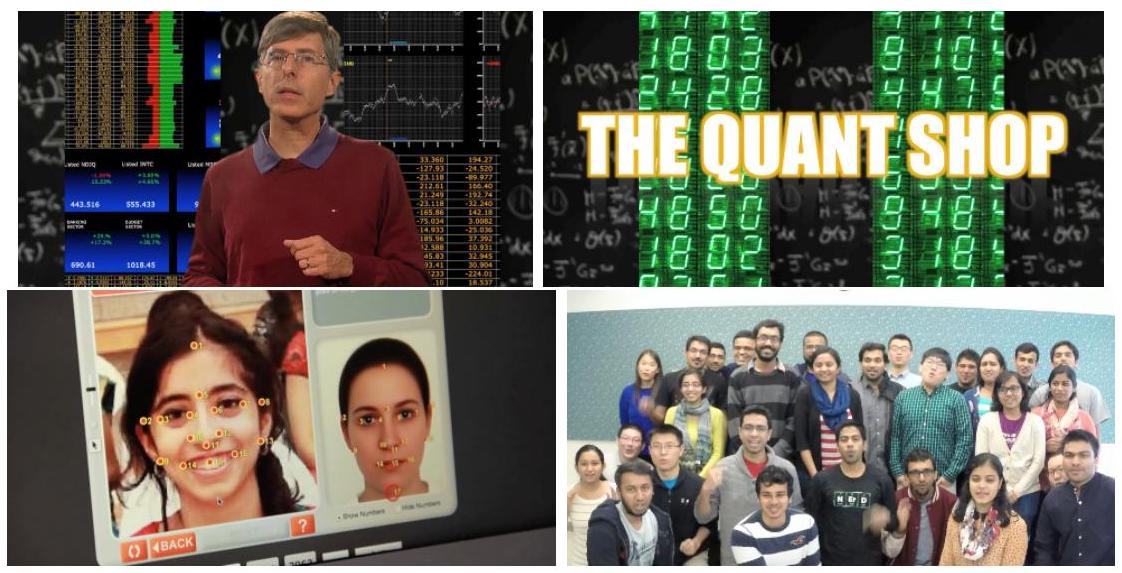
\includegraphics[max width=\textwidth]{2025_03_17_ca60ec0bfd96dcf8e028g-036}
\caption{Exciting \textenglish{scenes} \textenglish{from} \textenglish{data} \textenglish{science} television: \textenglish{The} \textenglish{Quant} Shop.}
\end{figure}

\begin{itemize}
  \item \textit{बाजार का खेल} - हे \textenglish{edge} फंड क्वांट्स तब अमीर हो जाते हैं जब वे कल की कीमतों का सही अनुमान लगाते हैं, और जब गलत होते हैं तब गरीब बन जाते हैं। हम सोने और तेल की भविष्य की कीमतों को अतीत की मूल्य डेटा का उपयोग करके कितनी सटीकता से अनुमानित कर सकते हैं? एक सफल मूल्य मॉडल बनाने में और कौनसी जानकारी शामिल होती है?
\end{itemize}

मैं आपको \textit{द क्वांट शॉप} के कुछ एपिसोड देखने के लिए प्रोत्साहित करता हूँ जब आप इस पुस्तक को पढ़ रहे हों। हम इसे मजेदार बनाने की कोशिश करते हैं, हालांकि मुझे यकीन है कि आपको इसमें कुछ असहज चीजें भी मिलेंगी। हर शो तीस मिनट तक चलता है, और शायद यह आपको आपकी अपनी भविष्यवाणी चुनौती को उठाने के लिए प्रेरित करे।

ये प्रोग्राम निश्चित रूप से आपको इन आठ विशिष्ट चुनौतियों के बारे में अधिक अंतर्दृष्टि देंगे। मैं इस किताब में इन परियोजनाओं का उपयोग महत्त्वपूर्ण पाठों को दर्शाने के लिए करूंगा, कि आकड़ों का विज्ञान कैसे किया जाए, सकारात्मक और नकारात्मक उदाहरणों दोनों के रूप में। ये परियोजनाएं एक प्रयोगशाला प्रदान करती हैं यह देखने के लिए कि कैसे समझदार लेकिन अनुभवहीन लोग, जो आपसे बहुत अलग नहीं हैं, आकड़ों के विज्ञान की समस्या के बारे में सोचते हैं, और जब उन्होंने ऐसा किया तो क्या हुआ।

\subsection{काग्गल चुनौतीयाँ}

एक अन्य प्रेरणा का स्रोत \textenglish{Kaggle} (\href{http://www.kaggle.com}{www.kaggle.com}) की चुनौतियाँ हैं, जो डेटा वैज्ञानिकों के लिए एक प्रतियोगी मंच प्रदान करता है। नई चुनौतियाँ नियमित रूप से पोस्ट की जाती हैं, जिनमें एक समस्या परिभाषा, प्रशिक्षण डेटा, और छुपे हुए मूल्यांकन डेटा पर एक स्कोरिंग फ़ंक्शन शामिल होता है। एक नेता बोर्ड सबसे मजबूत प्रतियोगियों के स्कोर को प्रदर्शित करता है, ताकि आप देख सकें कि आपका मॉडल आपके प्रतिद्वंद्वियों की तुलना में कितना अच्छा है। विजेता पोस्ट-प्रतियोगिता साक्षात्कारों के दौरान अपने मॉडलिंग रहस्यों का खुलासा करते हैं, ताकि आप अपनी मॉडलिंग कौशल को सुधार सकें।

कागल चुनौतियों में अच्छा प्रदर्शन करना आपके जीवनवृत्ति पर एक उत्कृष्ट प्रमाण पत्र है जो आपको डेटा वैज्ञानिक के रूप में अच्छी नौकरी पाने में मदद कर सकता है। सच में, संभावित नियोक्ता आपको खोज लेंगे यदि आप वास्तव में कागल के सितारे हैं। लेकिन असली कारण भाग लेने का है कि समस्याएं मजेदार और प्रेरणादायक हैं, और अभ्यास आपको एक बेहतर डेटा वैज्ञानिक बनाने में मदद करता है।

प्रत्येक अध्याय के अंत में दिए गए अभ्यास समाप्त हुए \textenglish{Kaggle} चुनौतियों की ओर संकेत करते हैं, जो उस अध्याय की सामग्री से थोड़ी जुड़ी होती हैं। यह चेतावनी दी जाती है कि \textenglish{Kaggle} एक भ्रामक ग्लैमरस दृष्टिकोण प्रस्तुत करता है डेटा विज्ञान का जो मशीन लर्निंग को लागू करता है, क्योंकि यह अत्यंत स्पष्ट रूप से परिभाषित समस्याएँ प्रस्तुत करता है जिसमें डेटा संग्रह और सफाई का कठिन कार्य पहले से ही आपके लिए किया गया होता है। फिर भी, मैं आपको प्रेरणा के लिए इसे देखने और नए परियोजनाओं के लिए डेटा के स्रोत के रूप में इसका उपयोग करने के लिए प्रोत्साहित करता हूँ।

\section{युद्ध कहानियों के बारे में}

प्रतिभा और विवेक दो अलग-अलग बौद्धिक उपहार हैं। \textit{प्रतिभा}सही उत्तर खोजने में दिखती है, कल्पनाशील मानसिक छलांगों में दिखती है जो बाधाओं और चुनौतियों को पार करती हैं। \textit{विवेक}पहले से ही बाधाओं से बचने में दिखता है, एक दिशा का अहसास या मार्गदर्शक प्रकाश प्रदान करने में दिखता है जो हमें सही दिशा में सुचारू रूप से आगे बढ़ाता है।

%---- \textenglish{Page} \textenglish{End} \textenglish{Break} \textenglish{Here} ---- \textenglish{Page} : 19

% \textenglish{Chapter} 1: \textenglish{What} \textenglish{is} \textenglish{Data} Science?

प्रतिभा तकनीकी शक्ति और गहराई में प्रकट होती है, चीजों को देखने और उन्हें करने की क्षमता जो अन्य लोग नहीं कर सकते। इसके विपरीत, ज्ञान अनुभव और सामान्य ज्ञान से आता है। यह दूसरों को सुनने से आता है। ज्ञान विनम्रता से आता है, यह देखने से कि आप कितनी बार पहले गलत रहे हैं और यह समझने से क्यों आप गलत थे, ताकि आप भविष्य के जालों को बेहतर तरीके से पहचान सकें और उनसे बच सकें।

डेटा साइंस, जीवन में अधिकांश चीजों की तरह, बुद्धिमानी से अधिक लाभान्वित होता है बजाय कि प्रतिभा से। इस किताब में, मैं उस बुद्धिमानी को साझा करने की कोशिश कर रहा हूँ जो मैंने कठिनाई से विभिन्न परियोजनाओं पर काम करके प्राप्त की है:\textit{युद्ध की कहानियाँ}।

\begin{itemize}
  \item \textit{विशाल-स्तरीय पाठ विश्लेषण और एनएलपी}: मेरा डाटा विज्ञान प्रयोगशाला स्टोनी ब्रुक यूनिवर्सिटी में बड़े डाटा पर विभिन्न परियोजनाओं पर काम करता है, जिसमें सोशल मीडिया से भावनात्मक विश्लेषण, ऐतिहासिक प्रवृत्तियों का विश्लेषण, प्राकृतिक भाषा प्रसंस्करण (एनएलपी) के लिए डीप लर्निंग दृष्टिकोण और नेटवर्क से विशेषता निष्कर्षण शामिल हैं।
  
  \item \textit{स्टार्ट-अप कंपनियाँ}: मैंने दो डाटा विश्लेषण कंपनियों, जनरल सेंटिमेंट और थ्राइवमेट्रिक्स के सह-संस्थापक और मुख्य वैज्ञानिक के रूप में सेवा की। जनरल सेंटिमेंट ने समाचार, ब्लॉग्स और सोशल मीडिया से बड़े पैमाने पर पाठ धाराओं का विश्लेषण किया ताकि लोगों, स्थानों, और चीजों से संबंधित भावनाओं (सकारात्मक या नकारात्मक) के रुझानों की पहचान की जा सके। थ्राइवमेट्रिक्स ने इस प्रकार के विश्लेषण को आंतरिक कॉर्पोरेट संचार, जैसे ईमेल और संदेश प्रणाली, पर लागू किया। इन उपक्रमों ने मुझे पुस्तक के रॉयल्टी से दूर जाने के लिए पर्याप्त धनी नहीं बनाया, लेकिन उन्होंने मुझे क्लाउड-आधारित कंप्यूटिंग सिस्टम पर अनुभव प्रदान किया, और उद्योग में कैसे डाटा का उपयोग होता है, इस पर अंतर्दृष्टि दी।\index{autocorrelation}\index{cicada}\index{fast \textenglish{Fourier} transform}\index{FFT}\index{logarithm}
  
  \item \textit{वास्तविक वैज्ञानिकों के साथ सहयोग}: मेरी बायोलॉजिस्ट्स और सामाजिक वैज्ञानिकों के साथ कई दिलचस्प सहयोग रहे हैं, जिन्होंने वास्तविक डाटा के साथ काम करने की जटिलताओं को समझने में मेरी सहायता की। प्रायोगिक डेटा अत्यंत शोर और त्रुटियों से भरा होता है, फिर भी आपको जो है उससे सर्वश्रेष्ठ करने का प्रयास करना होता है, ताकि यह खोजा जा सके कि दुनिया कैसे काम करती है।
  
  \item \textit{जुआ प्रणालियाँ बनाना}: एक विशेष रूप से मनोरंजक परियोजना जै-अलै मैचों के परिणामों की भविष्यवाणी करने लिए एक प्रणाली बनाना था ताकि हम उन पर दांव लगा सकें, इस अनुभव को मेरी पुस्तक \textit{कैल्क्युलेटेड बेट्स: कंप्यूटर, गैंबलिंग, और गणितीय मॉडलिंग टू विन} \cite{skiena2001calculated} में बताया गया है। हमारी प्रणाली डेटा संग्रह के लिए वेब स्क्रैपिंग, सांख्यिकीय विश्लेषण, सिमुलेशन/मॉडलिंग, और सावधानीपूर्वक मूल्यांकन पर निर्भर करती थी। हमने सामाजिक मीडिया विश्लेषण का उपयोग करके मूवी ग्रॉसेस \cite{zhang2009improving}, स्टॉक प्राइस \cite{zhang2010trading}, और फुटबॉल खेलों \cite{hong2010wisdom} के लिए भी भविष्यवाणी मॉडल विकसित और मूल्यांकन किया है।
  
  \item \textit{ऐतिहासिक व्यक्तियों की रैंकिंग}: विकिपीडिया का विश्लेषण करके 800,000 से अधिक ऐतिहासिक व्यक्तियों पर अर्थपूर्ण चर निकालने के लिए, हमने उन्हें ऐतिहासिक मीम्स के रूप में उनकी ताकत के अनुसार रैंक करने के लिए एक स्कोरिंग फंक्शन विकसित किया। यह रैंकिंग सबसे महान (जीसस, नेपोलियन, शेक्सपियर, मोहम्मद, और लिंकन शीर्ष पाँच में शामिल हैं) को कम महान लोगों से अलग करने का बेहतरीन काम करती है, और यह हमारी पुस्तक \textit{हूज़ बिगर?: व्हेयर हिस्टोरिकल फिगर्स रियली रैंक} \cite{skiena2013bigger} के लिए आधार के रूप में सेवा की।
\end{itemize}

इस पुस्तक में मैं जो सिखाता हूँ वह सभी अनुभव से उत्पन्न होता है, विशेष रूप से वे कहानियाँ जिन्हें मैं युद्ध कथाओं के रूप में वर्णित करता हूँ। \textit{इनमें से हर एक युद्ध कथा सच्ची है।} बेशक, कहानियाँ दोबारा सुनाने में कुछ हद तक सुधार पाती हैं, और संवाद को ज़्यादा दिलचस्प बनाने के लिए थोड़ा तकनीकी बना दिया गया है। फिर भी, मैंने समस्या को एक कच्चे मुद्दे से समाधान तक ले जाने की प्रक्रिया को ईमानदारी से ट्रेस करने की कोशिश की है, ताकि आप देख सकें कि यह कैसे उभरी।

\section{युद्ध कथा: सही प्रश्न का उत्तर देना}
स्टोनी ब्रुक यूनिवर्सिटी में हमारे अनुसंधान समूह ने एक एनएलपी-आधारित सिस्टम विकसित किया \index{NLP-based system}जो लाखों समाचार, ब्लॉग और सोशल मीडिया संदेशों का विश्लेषण करने के लिए है, और इन पाठों को चर्चा में शामिल सभी संस्थाओं के रुझानों में घटाने का काम करता है। पाठ प्रवाह (वॉल्यूम) में प्रत्येक नाम के उल्लेख की संख्या गिनना, सैद्धांतिक रूप से आसान है। किसी विशेष संदर्भ के अर्थ का सकारात्मक या नकारात्मक होना (रुचनात्मक विश्लेषण) निर्धारित करना कठिन है। लेकिन हमारा सिस्टम इस काम में काफी अच्छा था, विशेष रूप से जब कई संदर्भों पर समग्र रूप से देखा गया।\index{normalizing \textenglish{skewed} distribution}

यह तकनीक एक सामाजिक मीडिया विश्लेषण कंपनी के लिए नींव के रूप में काम की, जिसका नाम जनरल सेंटिमेंट था। यह देखना रोमांचक था कि कैसे एक स्टार्ट-अप शुरू हो रहा है, धन जुटाने, कर्मियों की भर्ती और नए उत्पादों के विकास की चुनौतियों का सामना कर रहा है।

लेकिन शायद सबसे बड़ी समस्या जो हमने सामना की वह सही प्रश्न का उत्तर देना था। जनरल सेंटिमेंट प्रणाली ने भावना और मात्रा के रुझानों को दर्ज किया \textit{हर} व्यक्ति, स्थान, और वस्तु के लिए जो कभी भी समाचार, ब्लॉग, और सोशल मीडिया में उल्लेखित की गई थी: 20 मिलियन से अधिक विभिन्न संस्थाएं। हमने हस्तियों और राजनेताओं की प्रतिष्ठा पर नज़र रखी। हमने कंपनियों और उत्पादों की किस्मत पर नज़र रखी। हमने खेल टीमों के प्रदर्शन को ट्रैक किया, और फिल्मों के बारे में चर्चा को पकड़ा। हम कुछ भी कर सकते थे!

लेकिन यह पता चलता है कि कोई भी आपको कुछ भी करने के लिए भुगतान नहीं करता है। वे आपको\textit{कुछ} करने के लिए भुगतान करते हैं, उनकी किसी विशेष समस्या को हल करने के लिए, या उनके व्यापार में किसी विशिष्ट परेशानी को दूर करने के लिए। कुछ भी करने में सक्षम होना एक भयानक बिक्री रणनीति साबित होती है, क्योंकि यह आपको हर ग्राहक के लिए उस ज़रूरत को फिर से खोजने की आवश्यकता होती है।

फेसबुक ने सितंबर 2006 तक दुनिया के लिए \textit{खुला}नहीं था। इसलिए जब जनरल सेंटिमेंट 2008 में शुरू हुआ, तो हम सोशल मीडिया युग की बिलकुल शुरुआत में थे। हमारे पास प्रमुख ब्रांडों और विज्ञापन एजेंसियों से बहुत रुचि थी, जो\textit{जानते}थे कि सोशल मीडिया विस्फोट के लिए तैयार है। वे \textit{जानते}थे कि यह नया आविष्कार महत्वपूर्ण था, और उन्हें वहां होना चाहिए। वे ⸨जानते⸩थे कि सोशल मीडिया डेटा का सही विश्लेषण उन्हें यह समझने में ताजगी भरी जानकारी दे सकता है कि उनके ग्राहक क्या सोच रहे थे। लेकिन वे यह नहीं ⸨जानते⸩थे कि वास्तव में उन्हें क्या जानना चाहिए।

अन्य विमान इंजन निर्माता इस बात में बहुत रुचि रखते थे कि बच्चे फेसबुक पर उनके बारे में कितना बात करते हैं। हमें उन्हें धीरे-धीरे यह बताना पड़ा कि उत्तर शून्य था। अन्य संभावित ग्राहक इस बात के प्रमाण की मांग करते थे कि हम

%---- \textenglish{Page} \textenglish{End} \textenglish{Break} \textenglish{Here} ---- \textenglish{Page} : 21



थे नीलसन टेलीविजन रेटिंग्स से अधिक सटीक। परंतु, बेशक, यदि आप नीलसन रेटिंग्स चाहते थे तो आपको उन्हें नीलसन से खरीदना चाहिए। हमारा सिस्टम एक बिल्कुल अलग दुनिया से अलग अंतर्दृष्टि प्रदान करता था। लेकिन आपको उन्हें उपयोग करने के लिए यह पता होना चाहिए था कि आप क्या चाहते हैं।

हमने विविध ग्राहकों के समूह से पर्याप्त ठेके पाने में सफलता हासिल की, जिसमें टोयोटा और ब्लैकबेरी जैसी उपभोक्ता ब्रांडे, हवाई पर्यटन कार्यालय जैसी सरकारी संगठन, और यहां तक कि 2012 में रिपब्लिकन उम्मीदवार मिट रोमनी के राष्ट्रपति अभियान भी शामिल हैं। हमारे विश्लेषकों ने उन्हें व्यापार की विविध समस्याओं पर अंतर्दृष्टि प्रदान की:

\begin{itemize}
  \item लोगों ने हवाई के बारे में क्या सोचा? (उत्तर: उन्हें लगता है कि यह घूमने के लिए बहुत अच्छी जगह है।)
  \item टोयोटा कारों में गंभीर ब्रेक समस्याओं की खबरों के बाद उनकी धारणाएँ कितनी जल्दी सुधरेंगी? (उत्तर: लगभग छह महीने।)
  \item लोगों ने ब्लैकबेरी के नए फोन मॉडल के बारे में क्या सोचा? (उत्तर: उन्हें आईफोन अधिक पसंद आया।)
  \item रॉमनी की धारणाएँ कितनी जल्दी सुधरेंगी, जब उन्होंने एक रिकॉर्डेड भाषण में 47\% मतदाताओं का अपमान किया? (उत्तर: कभी नहीं।)
\end{itemize}

लेकिन प्रत्येक बिक्री के लिए एक नए ब्रह्मांड में प्रवेश करना पड़ता था, जिसमें हमारे बिक्री स्टाफ और अनुसंधान विश्लेषकों के हिस्से पर काफी प्रयास और कल्पना शामिल होती थी। हम कभी भी एक ही उद्योग में दो ग्राहकों को शामिल करने में सफल नहीं हो सके, जिससे हमें पैमाने और संचित ज्ञान से लाभ हो सकता था।

बिल्कुल, ग्राहक हमेशा सही होता है। यह हमारी गलती थी कि हम उन्हें हमारी टेक्नोलॉजी का इस्तेमाल करने के सबसे अच्छे तरीके को समझा नहीं सके। ⸨यहां⸩ ⸨सीख⸩ यह है कि सिर्फ एक नए डेटा स्रोत के लिए दुनिया आपके दरवाजे पर नहीं आएगी। आपको डेटा को पैसों में बदलने से पहले सही प्रश्न पेश करने में सक्षम होना चाहिए।

\section{अध्याय नोट्स}
बेसबॉल खिलाड़ियों के ऐतिहासिक रिकॉर्ड का उपयोग करके यह दिखाने का विचार कि बाएँ हाथ से काम करने वालों की आयु कम होती है, हैलपर्न और कोरेन~\cite{halpern1991handedness} का है, लेकिन उनका निष्कर्ष विवादास्पद है। जनसंख्या में बाएँ हाथ से काम करने वालों का प्रतिशत तेजी से बढ़ रहा है, और देखे गए प्रभाव शायद जीवित रहने के पूर्वाग्रह का परिणाम हो सकते हैं~\cite{mcmanus2004right}। इसलिए, बाएं हाथ से काम करने वाले लोगों, डटे रहो! पूर्ण प्रकटीकरण: मैं आप में से एक हूँ।

क्वांटिटेटिव बेसबॉल विश्लेषण के क्षेत्र को कभी-कभी \textit{सेबरमेट्रिक्स} कहा जाता है, और इसके अग्रणी विशेषज्ञ बिल जेम्स नामक व्यक्ति हैं। मैं उभरते डेटा वैज्ञानिकों को उनकी \textit{हिस्टॉरिकल बेसबॉल एब्स्ट्रैक्ट}~\cite{james2010new} पढ़ने की सिफारिश करता हूँ, जो यह दिखाने का उत्कृष्ट उदाहरण है कि कैसे संख्या को ज्ञान और समझ में बदला जा सकता है। \textit{टाइम मैगज़ीन} ने कभी जेम्स के बारे में कहा था: "उन्हें पढ़ने का बहुत सा आनंद इस तथ्य से आता है कि एक प्रथम-श्रेणी बुद्धिमत्ता बेसबॉल पर खुद को बर्बाद कर रही है।" मैं \href{http://sports-reference.com}{http://sports-reference.com} को धन्यवाद देता हूँ उनकी वेबसाइट की छवियों को इस पुस्तक में उपयोग करने की अनुमति देने के लिए। और साथ ही ऐमेज़ॉन को, जो \textenglish{IMDb} का मालिक है।

न्यूयॉर्क में राइड-शेयरिंग प्रणालियों की संभावना का अध्ययन सैंटी और उनके सहयोगियों द्वारा किया गया था\cite{SRS14}, जिन्होंने दिखाया कि लगभग 95\% यात्राएं साझा की जा सकती थीं, प्रत्येक यात्रा में पाँच मिनट से अधिक विलंब नहीं होने पर।\index{exercises}

द लिडिया प्रणाली भाव विश्लेषण के लिए \cite{godbole2007large} में वर्णित है। शब्द अर्थ में परिवर्तन की पहचान करने के तरीके, जैसे \textenglish{Google} \textenglish{Ngram} के ऐतिहासिक पाठ संग्रह का विश्लेषण, \cite{kulkarni2015statistically} में रिपोर्ट किए गए हैं।

\section{व्यायाम}
\index{exercises}\subsection{डेटा सेट की पहचान}

\item\href{http://data.gov}{http://data.gov} पर जाएं, और पाँच डेटा सेट पहचानें जो आपको रोचक लगते हैं। प्रत्येक के लिए एक संक्षिप्त वर्णन लिखें, और तीन रोचक चीजें प्रस्तावित करें जो आप उनके साथ कर सकते हैं।
\end{enumerate}

\subsection{प्रश्न पूछना}

\begin{enumerate}
    \item निम्नलिखित डेटा स्रोतों में से प्रत्येक के लिए, तीन रोचक प्रश्न प्रस्तावित करें जिन्हें आप उनका विश्लेषण करके उत्तर दे सकते हैं:
    \begin{itemize}
        \item क्रेडिट कार्ड बिलिंग डेटा।
    \end{itemize}
\end{enumerate}

%---- \textenglish{Page} \textenglish{End} \textenglish{Break} \textenglish{Here} ---- \textenglish{Page} : 23

\section{कार्यान्वयन परियोजनाएँ}

\begin{enumerate}[resume]
    \item एक प्रोग्राम लिखें जो \href{http://Amazon.com}{Amazon.com} पर किसी पुस्तक के बेस्ट-सेलर रैंक को स्क्रैप करे। इसका उपयोग सभी स्किएना की पुस्तकों की रैंक को समय के साथ दिखाने के लिए करें। इनमें से कौनसी पुस्तक अगली वस्तु होनी चाहिए जिसे आप खरीदें? क्या आपके मित्र हैं जिनके लिए ये एक स्वागत योग्य और उपयुक्त उपहार हो सकता है? :-)
    
    \item अपने पसंदीदा खेल (बेसबॉल, फुटबॉल, बास्केटबॉल, क्रिकेट, या सॉकर) के लिए सभी मुख्य प्रतिभागियों के ऐतिहासिक सांख्यिकी रिकॉर्ड के साथ एक डेटा सेट की पहचान करें। प्रत्येक स्थिति में सर्वश्रेष्ठ खिलाड़ी की पहचान के लिए एक रैंकिंग प्रणाली तैयार करें और लागू करें।
\end{enumerate}

\section{साक्षात्कार प्रश्न}

\begin{enumerate}[फिर से शुरू करें]
    \item निम्नलिखित प्रश्नों में से प्रत्येक के लिए: (1) केवल अपनी दुनिया की समझ के आधार पर एक त्वरित अनुमान बनाएं, और फिर (2) गूगल का उपयोग करके समर्थनीय संख्याएँ खोजें और उनसे एक अधिक सैद्धांतिक अनुमान उत्पन्न करें। आपके दोनों अनुमानों में कितना अंतर था?
    \begin{enumerate}
        \item पूरे विश्व में कितने पियानो ट्यूनर हैं?
        \item आइस हॉकी रिंक पर बर्फ का वजन कितना होता है?
        \item संयुक्त राज्य अमेरिका में कितने गैस स्टेशन हैं?
        \item रोज़ाना कितने लोग ला गार्डिया एयरपोर्ट से आते-जाते हैं?
        \item संयुक्त राज्य अमेरिका में प्रत्येक वर्ष कितने गैलन आइसक्रीम बेची जाती है?
        \item नेशनल बास्केटबॉल एसोसिएशन (\textenglish{NBA}) द्वारा हर साल कितनी बास्केटबॉल खरीदी जाती हैं?
        \item विश्व के सभी महासागरों में कितनी मछलियाँ हैं?
        \item अभी पूरे विश्व में कितने लोग हवाई जहाज में उड़ रहे हैं?
        \item एक बड़े कमर्शियल जेट में कितनी पिंग-पोंग बॉल्स समा सकती हैं?
        \item आपके पसंदीदा देश में कितने मील पक्की सड़कें हैं?
        \item स्टोनी ब्रूक विश्वविद्यालय में सभी लोगों के वॉलेट में कितने डॉलर बिल्स हैं?
        \item एक सामान्य गैस स्टेशन प्रतिदिन कितने गैलन गैसोलीन बेचता है?
        \item इस पुस्तक में कितने शब्द हैं?
        \item न्यूयॉर्क शहर में कितनी बिल्लियाँ रहती हैं?
        \item स्टारबक्स की कॉफी से एक सामान्य कार का गैस टैंक भरने में कितनी लागत आएगी?
        \item चीन में कितनी चाय है?
        \item संयुक्त राज्य अमेरिका में कितने चेकिंग अकाउंट हैं?
    \end{enumerate}


\itemRegression और \textenglish{Classification} में क्या अंतर है?
    
\itemआप डेटा-चालित \textenglish{Recommendation} प्रणाली कैसे बनाएंगे? इस दृष्टिकोण की सीमाएँ क्या हैं?\index{Babbage, Charles}\index{data munging}\index{data science!languages}\index{programming languages}
    
\itemआप डेटा विज्ञान में रुचि कैसे लेने लगे?
    
\itemक्या आपको लगता है कि डेटा विज्ञान एक कला है या विज्ञान?
\end{enumerate}

% Mismatched: \sectionname{Kaggle Challenges}

\begin{enumerate}[फ़िर से शुरू करें]
    \item कौन टाइटैनिक के जहाज़ के हादसे से बच गया? \url{https://www.kaggle.com/c/titanic}
   
    \item एक विशेष टैक्सी कहाँ जा रही है? \url{https://www.kaggle.com/c/pkdd-15-predict-taxi-service-trajectory-i}
    
    \item एक दी गई टैक्सी यात्रा में कितना समय लगेगा? \url{https://www.kaggle.com/c/pkdd-15-taxi-trip-time-prediction-ii}
\end{enumerate}

%---- \textenglish{Page} \textenglish{End} \textenglish{Break} \textenglish{Here} ---- \textenglish{Page} : 25

\chapter{गणितीय प्रारंभिक बातें}
\section{प्रायिकता}
\index{probability}एक डेटा वैज्ञानिक वह व्यक्ति होता है जो एक कंप्यूटर वैज्ञानिक की तुलना में अधिक सांख्यिकी जानता है और एक सांख्यिकीविद से अधिक कंप्यूटर विज्ञान जानता है।

\begin{quote}
  \textit{जोश ब्लूमेनस्टॉक}
\end{quote}

तुम्हें दौड़ने से पहले चलना सीखना चाहिए। उसी तरह, गणितीय परिपक्वता का एक निर्धारित स्तर है जिसकी आवश्यकता होती है इससे पहले कि तुम्हें संख्यात्मक डेटा के साथ कुछ अर्थपूर्ण करने का भरोसा किया जा सके।

इस पुस्तक को लिखने में, मैंने यह मान लिया है कि पाठक ने प्रायिकता और सांख्यिकी, रैखिक बीजगणित, और निरंतर गणित का कुछ स्तर का अनुभव प्राप्त किया होगा। मैंने यह भी मान लिया है कि उन्होंने शायद इसका अधिकांश हिस्सा भूल गए होंगे, या शायद हमेशा मूल भावना (क्यों चीजें महत्वपूर्ण हैं, और उन्हें कैसे उपयोग करें) को पेड़ों (परिभाषाओं, प्रमेयों, और संचालन की सभी विस्तृत जानकारी) के लिए नहीं देखा होगा।

यह अध्याय कुछ बुनियादी गणितीय अवधारणाओं की आपकी समझ को ताज़ा करने की कोशिश करेगा। मेरे साथ चलते रहें, और भविष्य के संदर्भ के लिए आवश्यकता होने पर अपने पुराने पाठ्यपुस्तकों को निकाल दें। गहरे अवधारणाओं को पुस्तक में आगे तब प्रस्तुत किया जाएगा जब हमें उनकी आवश्यकता होगी।

\subsection{प्रायिकता के मूलभूत सिद्धांत}
प्रायिकता का सिद्धांत घटनाओं की संभावना के बारे में तर्क करने के लिए एक औपचारिक ढांचा प्रदान करता है। क्योंकि यह एक औपचारिक अनुशासन है, इसलिए इसमें संबंधित परिभाषाओं की एक जटिलता है जो यह निर्दिष्ट करती है कि हम किस बारे में तर्क कर रहे हैं:



\[ 
  S=\{ (1,1),(1,2),(1,3),(1,4),(1,5),(1,6),(2,1),(2,2),(2,3),(2,4),(2,5),(2,6),
  (3,1),(3,2),(3,3),(3,4),(3,5),(3,6),(4,1),(4,2),(4,3),(4,4),(4,5),(4,6), 
  (5,1),(5,2),(5,3),(5,4),(5,5),(5,6),(6,1),(6,2),(6,3),(6,4),(6,5),(6,6)\} .
  \]
  
  \item \textenglish{An} \textit{event} $E$ \textenglish{is} \textenglish{a} \textenglish{specified} \textenglish{subset} \textenglish{of} \textenglish{the} \textenglish{outcomes} \textenglish{of} \textenglish{an} experiment. \textenglish{The} \textenglish{event} \textenglish{that} \textenglish{the} \textenglish{sum} \textenglish{of} \textenglish{the} \textenglish{dice} \textenglish{equals} 7 \textenglish{or} 11 (\textenglish{the} \textenglish{conditions} \textenglish{to} \textenglish{win} \textenglish{at} \textenglish{craps} \textenglish{on} \textenglish{the} \textenglish{first} \textenglish{roll}) \textenglish{is} \textenglish{the} \textenglish{subset}
  
  \[
  E=\{(1,6),(2,5),(3,4),(4,3),(5,2),(6,1),(5,6),(6,5)\}
  \]

\itemकिसी परिणाम की \textit{संभावना} $s$, जिसे $p(\textenglish{s})$ द्वारा दर्शाया जाता है, दो विशेषताओं वाला एक संख्या होती है:

\begin{itemize}
    \item प्रत्येक $s$ परिणाम के लिए सैम्पल स्पेस $S$ में, $0 \leq p(\textenglish{s}) \leq 1$।
    \item सभी परिणामों की संभावनाओं का योग एक होता है: $\sum_{s \in S} p(\textenglish{s})=1$।
  \end{itemize}


  यदि हम दो भिन्न निष्पक्ष पासे मानते हैं, तो सभी संभावित परिणामों$s\timesS$के लिए संभावना$p(\textenglish{s})=(1 / 6)\in(1 / 6) = 1 / 36$होती है।

\itemकिसी घटना$E$की संभावना प्रयोग के परिणामों की संभावनाओं के योग के बराबर होती है। इस प्रकार
  
\[
  p(\textenglish{E})=\sum_{s \in E}p(\textenglish{s})
\]

एक वैकल्पिक रूपांतरण घटना$\textit{E}$के \bar{पूरक} के संदर्भ में होता है, वह स्थिति जब $E$ घटित नहीं होती। तब

\[
  P(\textenglish{E})=1-P(\bar{E}) .
  \]

यह उपयोगी है, क्योंकि अक्सर सीधे$P(\textenglish{E})$की तुलना में$P(\bar{E})$का विश्लेषण करना आसान होता है।

\itemA\textit{संख्यात्मक चर}$V$संभाव्यता स्थान के परिणामों पर एक संख्यात्मक फ़ंक्शन है। फ़ंक्शन "दो पासों के मानों का योग"$(V((a, \textenglish{b}))=a+b)$2 से 12 के बीच एक पूर्णांक परिणाम उत्पन्न करता है। यह संख्यात्मक चर के मानों के संभावना वितरण को दर्शाता है। संभावना$P(V(\textenglish{s})=7)=1 / 6$, जैसा कि पहले दिखाया गया है, जबकि$P(V(\textenglish{s})=12)=1 / 36$।\index{C–language}\index{Excel}\index{Java}\index{Mathematica}\index{notebook environments}\index{Wolfram Alpha}

\itemएक\textit{यादृच्छिक चरों का अपेक्षित मान}जो एक नमूना स्थान पर परिभाषित होता है$V$,$E(\textenglish{V})$के रूप में परिभाषित होता है
  
$
  E(\textenglish{V})=$_{s \[ S}p(\textenglish{s})\sumV(\textenglish{s})
\in

\end{itemize}

सभी यह आप पहले देख चुके होंगे। लेकिन यह वह भाषा प्रदान करता है जिसका उपयोग हम संभावना और सांख्यिकी के बीच जोड़ने के लिए करेंगे। जो डेटा हम देखते हैं वह आमतौर पर देखे गए घटनाओं के गुणों को मापने से आता है। संभावना और सांख्यिकी का सिद्धांत इस डेटा का विश्लेषण करने के उपकरण प्रदान करता है।

\subsection{प्रायिकता बनाम सांख्यिकी}
प्रायिकता और सांख्यिकी गणित के संबंधित क्षेत्र हैं जो घटनाओं की सापेक्ष आवृत्ति का विश्लेषण करने से संबंधित हैं। फिर भी, यह देखने के तरीके में मूलभूत अंतर हैं कि वे दुनिया को कैसे देखते हैं:

\begin{itemize}
  \item \textit{प्रायिकता} भविष्य की घटनाओं की संभावना की भविष्यवाणी करने से संबंधित है, जबकि \textit{सांख्यिकी} पिछले घटनाओं की आवृत्ति के विश्लेषण से संबंधित है।
  \item प्रायिकता मुख्य रूप से गणित की एक सैद्धांतिक शाखा है, जो गणितीय परिभाषाओं के परिणामों का अध्ययन करती है। सांख्यिकी मुख्य रूप से गणित की एक व्यवहारिक शाखा है, जो असली दुनिया में अवलोकनों को समझने की कोशिश करती है।\index{CSV files}\index{XML}
\end{itemize}

दोनों विषय महत्वपूर्ण, प्रासंगिक और उपयोगी हैं। लेकिन वे अलग हैं, और गणितीय साक्ष्य की प्रासंगिकता को सही से समझने के लिए उनके बीच के अंतर को समझना अत्यंत आवश्यक है। कई जुआरी इस अंतर को न समझ पाने के कारण ठंडी और अकेली कब्र में चले गए हैं, जो कि संभावना और सांख्यिकी के बीच सही अंतर करने में विफल रहे।

यह भेद शायद अधिक स्पष्ट हो जाएगा यदि हम एक गणितज्ञ के विचार प्रक्रिया को देखें जब वह अपने पहले क्रैप्स खेल का सामना करती है:

\begin{itemize}
  \item यदि यह गणितज्ञ एक संभाव्यता विज्ञानी होती, तो वह पासे को देखती और सोचती "छह-पक्षीय पासा? पासे का प्रत्येक पक्ष समान संभावना से ऊपर आएगा। अब यदि मान लिया जाए कि प्रत्येक पक्ष $1 / 6$ की संभावना के साथ ऊपर आता है, तो मैं यह समझ सकती हूँ कि मेरे नष्ट होने की संभावना क्या है।"
  \item इसके बजाय अगर कोई सांख्यिकीविद पास से गुजरता, तो वह पासे को देखता और सोचता "मैं कैसे जानूं कि वे भार नहीं हैं? मैं कुछ समय देखूंगा, और यह ध्यान रखूंगा कि कितनी बार प्रत्येक संख्या आती है। फिर मैं तय कर सकता हूँ कि मेरे अवलोकन बराबर-प्रायिकता के चेहरे की धारणा के साथ संगत हैं या नहीं। एक बार जब मैं पर्याप्त रूप से आश्वस्त हो जाऊं कि पासे निष्पक्ष हैं, तो मैं एक संभाव्यता विज्ञानी को कॉल करूंगा कि मुझे कैसे दांव लगाना है यह बताने के लिए।"
\end{itemize}

सारांश में, संभावना सिद्धांत हमें एक दिए गए आदर्श दुनिया के परिणाम खोजने में सक्षम बनाता है, जबकि सांख्यिकीय सिद्धांत हमें यह मापने में सक्षम बनाता है कि हमारी दुनिया कितनी आदर्श है। सिद्धांत और व्यवहार के बीच यह लगातार तनाव ही कारण है कि सांख्यिकीविदों की तुलना में अनिश्चिततावादी खुश-मिजाज होते हैं, जबकि सांख्यिकीविद अक्सर द्वंद्व में रहने वाले व्यक्ति साबित होते हैं।

आधुनिक प्रायिकता सिद्धांत का पहले प्रादुर्भाव 1654 में फ्राँस के पासे टेबल से हुआ। शेवेलियर डे मेरे, एक फ्रेंच कुलीन, यह जानना चाहते थे कि किसी विशेष सट्टेबाजी खेल में खिलाड़ी या घर का लाभ होता है।\footnote{उन्हें वास्तव में यह जानने की ज़रूरत नहीं थी। घर का हमेशा लाभ होता है।} मूल संस्करण में, खिलाड़ी चार पासे फेंकता है, और जीतता है यदि उनमें से कोई भी 6 नहीं होता। यदि कम से कम एक 6 आता है, तो घर समान धन राशि पर शर्त जीतता है।

डे मरे ने इस समस्या की ओर फ्रेंच गणितज्ञों ब्लेज़ पास्कल और पियर डी फर्मात का ध्यान आकर्षित किया, जो प्रमुख रूप से फर्मात का अंतिम प्रमेय के स्रोत के रूप में प्रसिद्ध हैं। मिलकर, इन व्यक्तियों ने प्रायिकता सिद्धांत की मूल बातें निकालीं और इसी क्रम में यह स्थापित किया कि यह पासा खेल घर के पक्ष में है, जिसकी प्रायिकता$p=1-(5 / 6)^4\approx0.517$ है, जहाँ प्रायिकता$p=0.5$ यह दर्शाएगी कि खेल निष्पक्ष है, जिसमें घर ठीक आधे समय जीतता है।

\subsection{संयुक्त घटनाएं और स्वतंत्रता}
हम जटिल घटनाओं में रुचि लेंगे जो सरल घटनाओं$A$और$B$से प्राप्त की जाती हैं, जो परिणामी सेट पर होती हैं। संभवतः घटना$A$यह है कि कम से कम दो में से एक पासा सम संख्या हो, जबकि घटना$B$संकेत करती है कि कुल 7 या 11 हो। ध्यान दें कि$A$के कुछ विशेष परिणाम होते हैं जो$B$के परिणाम नहीं होते हैं, विशेष रूप से

\[\]

\begin{aligned}
A-B=\{ & (1,2),(1,4),(2,1),(2,2),(2,3),(2,4),(2,6),(3,2),(3,6),(4,1) \\\index{AOL}\index{company data}\index{data!collecting}\index{data sources}\index{protocol buffers}
& (4,2),(4,4),(4,5),(4,6),(5,4),(6,2),(6,3),(6,4),(6,6)\}
\end{aligned}

\]

यह सेट फर्क ऑपरेशन है। ध्यान दें कि यहाँ$B-A=\{\}$, क्योंकि हर जोड़ जो 7 या 11 बनाता है, उसमें एक विषम और एक सम संख्या शामिल होनी चाहिए।

$दोनों घटनाओं$A$और$B$के बीच सामान्य परिणामों को प्रतिच्छेदन कहा जाता है, जिसे \capA$B@ के रूप में निरूपित किया जाता है। इसे इस प्रकार लिखा जा सकता है:

\[ 
\textenglish{A} \cap B=A-(S-B) .
\]

तक ने जो परिणाम किसी$A$या$B$में प्रकट होते हैं उन्हें यूनियन कहा जाता है, जिसे$A\cupB$द्वारा सूचित किया जाता है। पूरक ऑपरेशन$\bar{A}=S-A$ के साथ, हमें घटनाओं को संयोजित करने के लिए एक समृद्ध भाषा मिलती है, जैसा चित्रा 2.1 में दिखाया गया है। हम इन परिभाषित सेटों में होने वाले परिणामों की संभावनाओं को जोड़कर आसानी से किसी भी सेट की संभावना की गणना कर सकते हैं।

इवेंट्स$A$और$B$तभी स्वतंत्र हैं जब और केवल जब

\[ 
P(\textenglish{A} \cap \textenglish{B})=P(\textenglish{A}) \times P(\textenglish{B})
\]

इसका मतलब यह है कि घटनाओं$A$और$B$के बीच कोई विशेष परिणाम संरचना साझा नहीं की गई है। मानते हुए कि मेरी कक्षा में आधे छात्राएं हैं, और मेरी कक्षा में आधे छात्र औसत से ऊपर हैं, तो अगर घटनाएँ स्वतंत्र हैं तो हम उम्मीद करेंगे कि मेरे छात्रों में से एक चौथाई छात्राएं हैं और वे औसत से ऊपर भी हैं।

\begin{figure}[h]
  \centering
  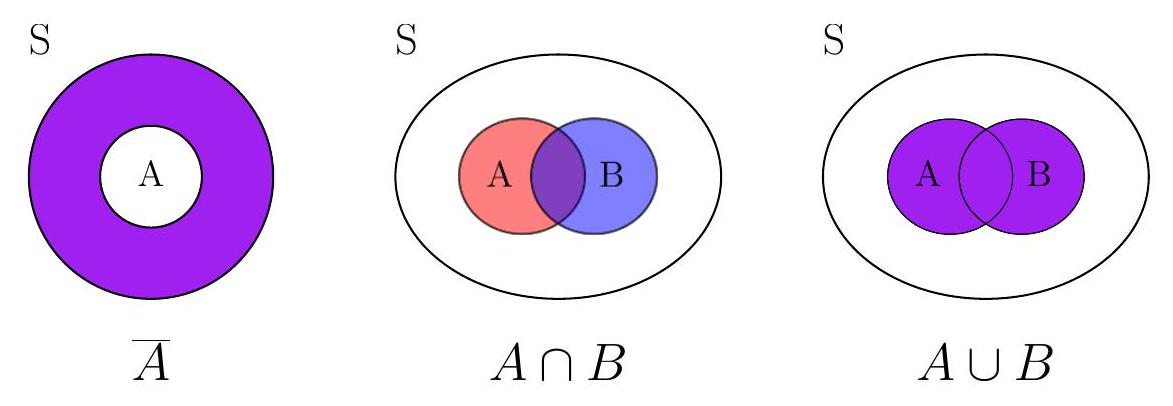
\includegraphics[max width=\textwidth]{2025_03_17_ca60ec0bfd96dcf8e028g-047}
  \caption{Venn \textenglish{diagrams} \textenglish{illustrating} \textenglish{set} \textenglish{difference} (\textenglish{left}), \textenglish{intersection} (\textenglish{middle}), \textenglish{and} \textenglish{union} (\textenglish{right}).}
\end{figure}

%---- \textenglish{Page} \textenglish{End} \textenglish{Break} \textenglish{Here} ---- \textenglish{Page} : 30



सांख्यिकी सिद्धांतकार स्वतंत्र घटनाएँ पसंद करते हैं, क्योंकि यह उनकी गणनाओं को सरल बनाता है। लेकिन डेटा वैज्ञानिक आमतौर पर ऐसा नहीं करते। जब किसी भविष्य की घटना$B$ की संभावना को पूर्व की घटना$A$ के ज्ञान के आधार पर अनुमानित करने के लिए मॉडल बनाते हैं, तब हम चाहते हैं कि$B$का$A$पर अधिकतम निर्भरता हो।

मान लीजिए कि मैं हमेशा छाता तभी इस्तेमाल करता हूँ जब बारिश हो रही होती है। मान लें कि यहाँ बारिश होने की संभावना (घटना$B$) है, जैसे कि,$p=1/5$। इसका अर्थ यह है कि मेरे पास छाता होने की संभावना (घटना$A$) है$q=1/5$। लेकिन और भी महत्वपूर्ण बात यह है कि अगर आपको बारिश की स्थिति पता है तो आप ठीक-ठीक बता सकते हैं कि मेरे पास छाता है या नहीं। ये दोनों घटनाएं पूरी तरह से\textit{संबद्ध}हैं।

इसके विपरीत, मान लीजिए कि घटनाएँ स्वतंत्र थीं। तब

\[
P(\textenglish{A} \mid \textenglish{B})=\frac{P(\textenglish{A} \cap \textenglish{B})}{P(\textenglish{B})}=\frac{P(\textenglish{A}) P(\textenglish{B})}{P(\textenglish{B})}=P(\textenglish{A})
\]

और यह कि बारिश हो रही है या नहीं, इसका बिल्कुल भी कोई प्रभाव नहीं पड़ता कि मैं अपना सुरक्षात्मक उपकरण लेकर चलता हूँ या नहीं।

संबंध भविष्यवाणी मॉडल्स के पीछे प्रेरक शक्ति होते हैं, इसलिए हम धारा 2.3 में चर्चा करेंगे कि उन्हें कैसे मापा जाए और उनका क्या मतलब होता है।

\subsection{सशर्त प्रायिकता}
जब दो घटनाएँ आपस में संबंधित होती हैं, तो उनके बीच एक निर्भरता होती है जो गणनाओं को और जटिल बना देती है।\textit{सशर्त प्रायिकता} \textenglish{A} की, जब \textenglish{B} दिया जाता है, P(A$B)$ इस प्रकार परिभाषित होती है:\index{academic data}\index{Google Scholar}\index{sweat equity}

\[
P(\textenglish{A} \mid \textenglish{B})=\frac{P(\textenglish{A} \cap \textenglish{B})}{P(\textenglish{B})}
\]

अनुच्छेद 2.1.2 से पासा फेंकने की घटनाओं को याद करें, अर्थात्:

\begin{itemize}
  \item घटना $A$ यह है कि दो पासों में से कम से कम एक सम संख्या होना चाहिए।
  \item घटना $B$ यह है कि दोनों पासों की योगफल या तो 7 या 11 है।
\end{itemize}

ध्यान दें कि$P(A\midB)=1$, क्योंकि कोई भी रोल जो विषम मान को जोड़ता है, उसमें एक सम और एक विषम संख्या शामिल होनी चाहिए। इस प्रकार$A\capB=B$, उपरोक्त छत्र मामले के समान।$P(B\midA) के लिए$, ध्यान दें कि$P(A\capB)=9/36$ और$P(\textenglish{A})=25/36$, इसलिए$P(B\midA)=9/25$।

शर्तीय प्रायिकता हमारे लिए महत्वपूर्ण होगी, क्योंकि हमें एक घटना$A$(संभवतः कि एक विशिष्ट ईमेल का टुकड़ा स्पैम है) की संभावना में रुचि है कुछ सबूत$B$(संभवतः दस्तावेज़ के भीतर शब्दों का वितरण) के रूप में। वर्गीकरण समस्याएँ सामान्यतः किसी न किसी प्रकार से शर्तीय प्रायिकताओं की गणना तक सीमित होती हैं।

हमारा मुख्य साधन सशर्त प्रायिकताएँ गणना करने के लिए बायेस प्रमेय होगा, जो निर्भरताओं की दिशा को उलट देता है:

\[
P(\textenglish{B} \mid \textenglish{A})=\frac{P(\textenglish{A} \mid \textenglish{B}) P(\textenglish{B})}{P(\textenglish{A})}
\]

अक्सर यह सिद्ध हो जाता है कि संभावनाओं की गणना एक दिशा में करना दूसरी दिशा से आसान होता है, जैसा कि इस समस्या में है। बेज़ थिओरम$P(B\midA)= (1\cdot9/36)/(25/36) = 9/25$ के अनुसार, ठीक वो मिला जो पहले मिला था। हम बेज़ थिओरम को अनुभाग 5.6 में पुनः देखेंगे, जहाँ यह साक्ष्य के सामने संभावनाओं की गणना के आधार की स्थापना करेगा।

\subsection{प्रायिकता वितरण}
\index{probability distribution}संभाव्य चर संख्यात्मक कार्य होते हैं जहां मूल्यों को घटित होने की प्रायिकताओं के साथ जोड़ा जाता है। हमारे उदाहरण में जब$V(\textenglish{s})$दो फेंके गए पासों का योग लिया जाता है, तो यह कार्य 2 और 12 के बीच एक पूर्णांक उत्पन्न करता है। किसी विशेष मूल्य$V(\textenglish{s})=X$की प्रायिकता उन सभी परिणामों की प्रायिकताओं का योग होती है जो मिलकर$X$बनाते हैं।

ऐसे यादृच्छिक चर को उनकी \textit{प्रायिकता घनत्व फलन}, या \textenglish{pdf} के द्वारा प्रदर्शित किया जा सकता है। यह एक ग्राफ है जहाँ पर$x$-अक्ष वह मान प्रदर्शित करता है जो यादृच्छिक चर ले सकता है, और$y$-अक्ष उस दिए गए मान की प्रायिकता को दर्शाता है। चित्र \ref{fig:pdf-cdf}(बाएँ) दो निर्दोष पासों के योग का \textenglish{pdf} प्रस्तुत करता है। देखिए कि$X=7$ पर शीर्षक सबसे अधिक बार आने वाले पासे के योग से मेल खाता है, जिसकी प्रायिकता$1/6$ है।

ऐसे पीडीएफ प्लॉट्स का डेटा फ़्रीक्वेंसी के हिस्टोग्राम्स के साथ एक मजबूत संबंध होता है, जहाँ $x$-अक्ष फिर से मूल्य की श्रेणी का प्रतिनिधित्व करता है, लेकिन $y$ अब यह दर्शाता है कि हर दिए गए मूल्य $X$ के लिए कितनी घटना समय को देखा गया। एक हिस्टोग्राम को पीडीएफ में परिवर्तित करने के लिए हर बकेट को सभी बकेट्स पर कुल फ़्रीक्वेंसी से विभाजित किया जा सकता है। तब प्रविष्टियों का योगफल 1 बन जाता है, इसलिए हमें एक प्रायिकता वितरण प्राप्त होता है।

हिस्टोग्राम सांख्यिकी होते हैं: वे परिणामों के वास्तविक अवलोकनों को दर्शाते हैं। इसके विपरीत, पीडीएफ संभाव्य होते हैं: वे यह प्रदर्शित करते हैं कि अगला अवलोकन मूल्य$X$ होगा। हम अक्सर प्रायोगिक रूप से अवलोकनों के हिस्टोग्राम$h(\textenglish{x})$ का उपयोग उन संभावनाओं को अनुमानित करने के लिए करते हैं \footnote{एक तकनीक जिसे डिस्काउंटिंग कहा जाता है, दुर्लभ घटनाओं की आवृत्ति का बेहतर अनुमान लगाने का एक तरीका प्रदान करती है, और धारा~\ref{sec:discounting} में चर्चा की जाएगी।} संपूर्ण अवलोकनों की संख्या द्वारा गिनती को सामान्यीकृत करके:\index{Aaron \textenglish{Schwartz} case}\index{data!logging}\index{Internet \textenglish{of} Things}\index{terms \textenglish{of} service}\index{web crawling}

\[
P(k=X)=\frac{h(k=X)}{\sum_{x} h(x=X)}
\]

एक और तरीका है जिससे यादृच्छिक चरों को प्रस्तुत किया जा सकता है, जिसे अक्सर उपयोगी साबित होने वाला कहा जाता है, जिसे \textit{समाकल घनत्व फलन} या \textenglish{cdf} कहा जाता है। \textenglish{cdf} पीडीएफ में संभावनाओं का संचयी योग होता है; यह $k$ के फलन के रूप में# इस बात की संभावना को दर्शाता है कि $X\leqk$ के बजाय इस बात की संभावना कि $X=k$। चित्र~\ref{चित्र:पीडीएफ-सीडीएफ}(दाईं) पासा योग वितरण का \textenglish{cdf} दिखाता है। मान बाईं से दाईं ओर एकाकी रूप से बढ़ते हैं, क्योंकि प्रत्येक पद पिछले योग में सकारात्मक संभावना जोड़ने से आता है। दाईं ओर का सबसे अधिक मान 1 होता है, क्योंकि सभी परिणाम अधिकतम से अधिक नहीं बने होते।

यह समझना महत्वपूर्ण है कि एक दिए गए रैंडम वेरिएबल$V$के pdf$P(\textenglish{V})$और cdf$C(\textenglish{V})$में बिल्कुल वही जानकारी होती है। हम इनके बीच आगे और पीछे जा सकते हैं क्योंकि:

\[
P(k=X)=C(\textenglish{X} \leq k+\delta)-C(\textenglish{X} \leq \textenglish{k})
\]

जहाँ $\delta=1$ पूर्णांक वितरणों के लिए। Cdf, \textenglish{pdf} का संचयी योग होता है, इसलिए

\[
C(\textenglish{X} \leq \textenglish{k})=\sum_{x \leq k} P(X=x)
\]

बस इस बात का ध्यान रखें कि आप किस वितरण को देख रहे हैं। ⸨क्यूमुलेटिव⸩ वितरण हमेशा दाएँ की ओर बढ़ने पर ऊँचे होते जाते हैं, और ⸨प्रॉबेबिलिटी⸩ $C(X\leq\infty)=1$ के साथ समाप्त होते हैं। इसके विपरीत, एक ⸨पीडीएफ⸩ के वक्र के नीचे कुल क्षेत्रफल 1 के बराबर होता है, इसलिए वितरण में किसी भी बिंदु पर ⸨प्रॉबेबिलिटी⸩ आमतौर पर काफी कम होती है।

\begin{figure}[h!]
    \centering
    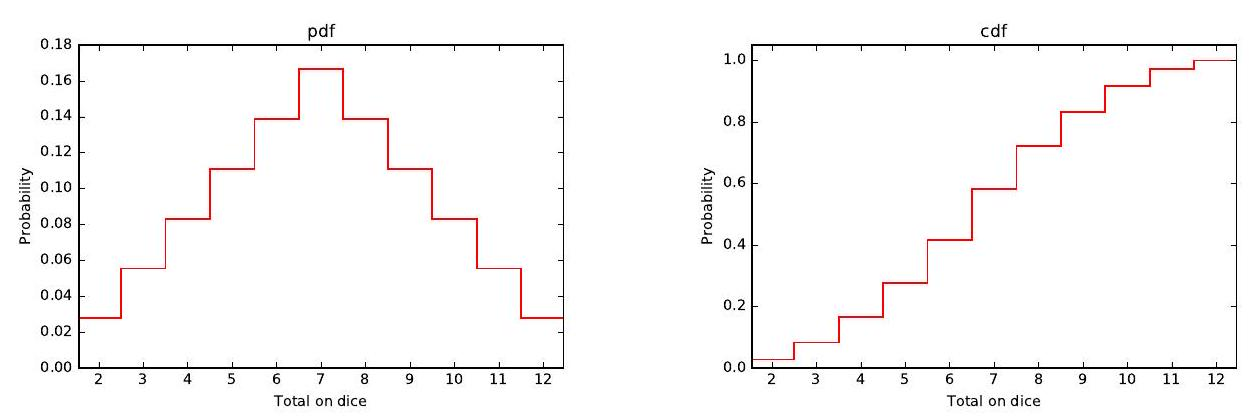
\includegraphics[max width=\textwidth]{2025_03_17_ca60ec0bfd96dcf8e028g-049}
    \caption{The \textenglish{probability} \textenglish{density} \textenglish{function} (\textenglish{pdf}) \textenglish{of} \textenglish{the} \textenglish{sum} \textenglish{of} \textenglish{two} \textenglish{dice} \textenglish{contains} \textenglish{exactly} \textenglish{the} \textenglish{same} \textenglish{information} \textenglish{as} \textenglish{the} \textenglish{cumulative} \textenglish{density} \textenglish{function} (\textenglish{cdf}), \textenglish{but} \textenglish{looks} \textenglish{very} different.}
    \label{fig:pdf-cdf}
\end{figure}

एक मजेदार उदाहरण संचयी और वृद्धिशील वितरणों के बीच भिन्नता का चित्रण चित्र~\ref{fig:iphone-sales} में दिखाया गया है। दोनों वितरण \textenglish{Apple} आईफोन बिक्री पर बिल्कुल समान डेटा दिखाते हैं, लेकिन \textenglish{Apple} के \textenglish{CEO} टिम कुक ने एक बड़े शेयरधारक कार्यक्रम में किस वक्र को प्रस्तुत करना चुना? संचयी वितरण (लाल) दिखाता है कि बिक्री तेजी से बढ़ रही है, है ना? लेकिन यह वृद्धि दर का भ्रामक दृष्टिकोण प्रस्तुत करता है, क्योंकि वृद्धिशील परिवर्तन इस कार्य का व्युत्पन्न है, और इसे देख पाना कठिन है। वास्तव में, तिमाही-दर-तिमाही बिक्री प्लॉट (नीला) यह दिखाता है कि प्रस्तुति से पहले की आखिरी दो अवधियों में आईफोन बिक्री दर वास्तव में घट गई थी।

\begin{figure}[h!]
    \centering
    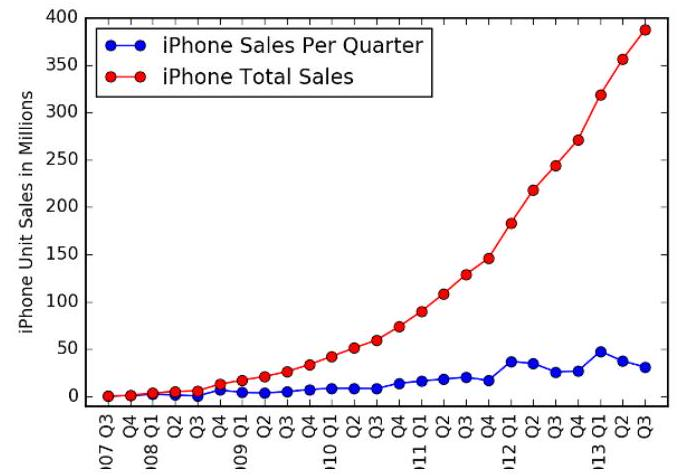
\includegraphics[max width=\textwidth]{2025_03_17_ca60ec0bfd96dcf8e028g-050}
    \caption{iPhone \textenglish{quarterly} \textenglish{sales} \textenglish{data} \textenglish{presented} \textenglish{as} \textenglish{cumulative} \textenglish{and} \textenglish{incremental} (\textenglish{quarterly}) distributions. \textenglish{Which} \textenglish{curve} \textenglish{did} \textenglish{Apple} \textenglish{CEO} \textenglish{Tim} \textenglish{Cook} \textenglish{choose} \textenglish{to} present?}
    \label{fig:iphone-sales}
\end{figure}

\section{वर्णनात्मक आँकड़े}
वर्णनात्मक आँकड़े दिए गए आँकड़ा सेट या नमूने की विशेषताओं को पकड़ने के तरीके प्रदान करते हैं। वे अवलोकित आँकड़ों को संक्षेप में प्रस्तुत करते हैं और इसके बारे में बात करने के लिए एक भाषा प्रदान करते हैं। जैसे कि औसत, न्यूनतम, गणना, या योग जैसे नए व्युत्पन्न तत्व द्वारा तत्वों के एक समूह का प्रतिनिधित्व करना एक बड़े आँकड़ा सेट को एक छोटे सार आँकड़े में कम कर देता है: आँकड़ा कमी के रूप में समेकन।\index{Pubmed}

ऐसे आँकड़े अपने आप में विशेषताएँ बन सकते हैं जब उन्हें पूरे डेटा सेट में प्राकृतिक समूहों या क्लस्टरों पर लिया जाता है। वर्णनात्मक आँकड़ों के दो मुख्य प्रकार हैं:

\begin{itemize}
  \item \textit{केंद्रीय प्रवृत्ति मापदंड}, जो उस केंद्र को पकड़ते हैं जिसके चारों ओर डेटा वितरित होता है। 
  \item \textit{भिन्नता} या \textit{परिवर्तनीयता मापदंड}, जो डेटा के फैलाव को वर्णित करते हैं, अर्थात माप केंद्र से कितनी दूर स्थित हैं। 
\end{itemize}

इन सांख्यिकी आँकड़ों को मिलाकर, यह हमारे वितरण के बारे में हमें बहुत सारी जानकारी देते हैं।

\subsection{केन्द्रता मापदंड}
स्कूल में सांख्यिकी का जो पहला तत्व हमें सिखाया जाता है, वह है बुनियादी केन्द्रता मापदंड: माध्य, माध्यिका, और प्रतिलोम। डेटा सेट को विश्लेषित करने के लिए एकल संख्या की कल्पना करते समय यहां से शुरू करना सही है।

\begin{itemize}
  \item \textit{औसत}: आप शायद \textit{अर्थमैटिक मीन} के उपयोग में काफी सहज हैं, जहाँ हम मूल्यों को जोड़ते हैं और अवलोकनों की संख्या से विभाजित करते हैं:
\end{itemize}

\[
\mu_{X}=\frac{1}{n} \sum_{i=1}^{n} x_{i}
\]

हम आसानी से औसत को प्रविष्टियों और विलोपन की धारा के तहत बनाए रख सकते हैं, मूल्य के योग को आवृत्ति गिनती से अलग रखकर, और केवल आवश्यकतानुसार विभाजित करके। औसत का विशेष महत्व है जब असमानताओं के बिना सममित वितरण को वर्णित किया जाता है, जैसे ऊँचाई और वजन। इसका सममित होना यह दर्शाता है कि औसत से ऊपर की वस्तुओं की संख्या औसतन नीचे की वस्तुओं की संख्या के लगभग समान होनी चाहिए।

%---- \textenglish{Page} \textenglish{End} \textenglish{Break} \textenglish{Here} ---- \textenglish{Page} : 34



कि यह बाहरी मूल्यों के बिना है, जिसका अर्थ है कि मूल्यों की सीमा समुचित रूप से तंग है। ध्यान दें कि एक अकेला \textenglish{MAXINT} जो सामान्यतः ठोस पर्यवेक्षण सेट में आता है, वह माध्य को बुरी तरह से प्रभावित कर सकता है। केंद्रीयता का एक माप होता है, जो ऐसी अनुचित वितरण में अधिक उपयुक्त साबित होता है।\index{data!compatibility}\index{unit conversions}

\subsubsection{ज्यामितीय औसत}

\textenglish{The} \emph{ज्योमितीय माध्य} $n$ मानों के गुणनफल की $n$वीं जड़ होती है:

$$
\left(\prod_{i=1}^{n}a_{i}\right)^{1 / n}=\sqrt[n]{a_{1} a_{2} \ldots a_{n}}
$$

ज्यामितीय माध्य हमेशा अंकगणितीय माध्य से कम या उसके बराबर होता है। उदाहरण के लिए, 36 पासों के रोल्स के योग का ज्यामितीय माध्य 6.5201 है, जबकि अंकगणितीय माध्य 7 है। यह शून्य के समीप के मूल्यों के लिए बहुत संवेदनशील होता है। शून्य का एकल मान ज्यामितीय माध्य को बेकार कर देता है: चाहे आपके डेटा में अन्य मान जो भी हों, आप शून्य पर आ जाते हैं। यह कुछ हद तक$\infty$एक अंकगणितीय माध्य में एक बाह्यक्षी के होने जैसा है। लेकिन जब अनुपातों का औसत निकालना होता है, तो ज्यामितीय माध्य अपनी उपयोगिता सिद्ध करता है।$1 / 2$और$2 / 1$का ज्यामितीय माध्य 1 है, जबकि माध्य 1.25 है। 1 से कम अनुपातों के लिए उपलब्ध "स्थान" 1 से अधिक अनुपातों की तुलना में कम होता है, जिससे एक विषमता पैदा होती है जिसे अंकगणितीय माध्य अधिक दर्शाता है। इन मामलों में, ज्यामितीय माध्य अधिक अर्थपूर्ण होता है, जैसे कि अनुपातों के\emph{लघुगणकों}का अंकगणितीय माध्य होता है।

\subsubsection{माध्यिका}

\emph{मीडियन} एक डेटा सेट के बीचों-बीच का सटीक मूल्य होता है; जितने तत्व ⸨मीडियन⸩ के ऊपर होते हैं, उतने ही नीचे होते हैं। जब आपके पास तत्वों की सम संख्या होती है, तब क्या ⸨मीडियन⸩ लिया जाए, इस पर थोड़ी बहस होती है। आप दो केंद्रीय उम्मीदवारों में से किसी एक को ले सकते हैं: किसी भी तर्कसंगत डेटा सेट में ये दोनों मान लगभग समान होने चाहिए। वास्तव में, पासे के उदाहरण में, दोनों ही 7 हैं।

माध्यिका की इस प्रकार परिभाषित एक अच्छी विशेषता यह है कि यह मूल डेटा स्ट्रीम का एक वास्तविक मान होना चाहिए। वास्तव में कोई व्यक्ति होता है जिसकी माध्यिका ऊँचाई होती है जिसे आप उदाहरण के रूप में इंगित कर सकते हैं, लेकिन शायद ही दुनिया में कोई व्यक्ति होता है जिसकी ऊँचाई \emph{सटीक रूप से} औसतन होती है। आप यह विशेषता खो देते हैं जब आप दो केंद्रीय तत्वों का औसत लेते हैं।

कौन सा सेंट्रलिटी माप अनुप्रयोगों के लिए सबसे अच्छा है? माध्यिका साधारणतः सममित वितरणों में अंकगणितीय माध्य के काफ़ी करीब होती है, लेकिन यह अक्सर देखना रोचक होता है कि वे कितनी दूर हैं, और माध्यिका किस ओर स्थित है।

माध्यिका आम तौर पर तिरछे वितरणों या चरम मानों वाले आँकड़ों के लिए बेहतर सांख्यिकी साबित होती है: जैसे धन और आय। बिल गेट्स संयुक्त राज्य अमेरिका की प्रति व्यक्ति धन की औसत को 250 बढ़ाते हैं, लेकिन माध्यिका पर कुछ भी नहीं। अगर वह आपको व्यक्तिगत रूप से अधिक धनी महसूस कराते हैं, तो आगे बढ़ें और औसत का उपयोग करें। लेकिन यहाँ माध्यिका अधिक सूचनात्मक सांख्यिकी है, जैसा कि यह किसी भी पावर लॉ वितरण के लिए होगी।



\subsubsection{मोड}
\index{mode}
\emph{मोड} डेटा सेट में सबसे अधिक बार आने वाला तत्व है। हमारे चल रहे पासे के उदाहरण में, यह 7 है, क्योंकि यह छत्तीस तत्वों में से छह बार आता है। ईमानदारी से कहूँ, तो मैंने कभी भी ⸨मोड⸩ को केंद्रीयता माप के रूप में बहुत कुछ समझ प्रदान करते नहीं देखा, क्योंकि यह अक्सर केंद्र के करीब नहीं होता है। एक बड़े रेंज में मापे गए नमूनों में किसी विशेष मान पर बहुत कम दोहराए गए तत्व या टकराव होने चाहिए। यह मोड को एक संयोग का मामला बनाता है। वास्तव में, सबसे अधिक बार आने वाले तत्व अक्सर डेटा सेट में कलाकृतियों या विसंगतियों को उजागर करते हैं, जैसे कि डिफ़ॉल्ट मान या त्रुटि कोड जो वास्तव में अंतर्निहित वितरण के तत्वों का प्रतिनिधित्व नहीं करते हैं। एक आवृत्ति वितरण (या हिस्टोग्राम) में शिखर की संबंधित अवधारणा अर्थपूर्ण होती है, लेकिन दिलचस्प शिखर केवल उचित बकेटिंग के माध्यम से ही प्रकट होते हैं। संयुक्त राज्य अमेरिका में वार्षिक वेतन वितरण का वर्तमान शिखर \$30,000 से \$40,000 प्रति वर्ष के बीच होता है, हालाँकि ⸨मोड⸩ सम्भवतः शून्य पर होता है।\index{character \textenglish{code} unification}\index{name unification}\index{numerical conversions}

\subsection{विविधता के माप}
\index{variability measures}
विविधता का सबसे सामान्य माप \emph{मानक विचलन}\index{standard deviation}$\sigma$ है, जो व्यक्तिगत तत्वों और औसत के बीच वर्गों के अंतर के योग को मापता है:

$$
\sigma=\sqrt{\frac{\sum_{i=1}^{n}\left(a_{i}-\bar{a}\right)^{2}}{n-1}}
$$

एक संबंधित सांख्यिकी, \emph{वैरिएंस} $V$, मानक विचलन का वर्ग होता है, अर्थात $V=\sigma^{2}$। कभी-कभी वैरिएंस के बारे में बात करना मानक विचलन की तुलना में अधिक सुविधाजनक होता है, क्योंकि यह शब्द आठ अक्षर छोटा होता है। लेकिन वे वास्तव में एक ही चीज़ को मापते हैं।

उदाहरण के लिए, विनम्र प्रकाश बल्ब पर विचार करें, जो आमतौर पर अपेक्षित कार्यकाल के साथ आता है, मान लें$\mu=3000$घंटे, जो किसी अंतर्निहित वितरण से उत्पन्न होता है जैसा कि चित्र 2.4 में दिखाया गया है। एक पारंपरिक बल्ब में, इसके लंबे समय तक चलने की संभावना$\mu$जल्दी खराब होने की संभावना के समान ही मानी जाती है, और इस अस्थिरता की मात्रा$\sigma$से मापी जाती है। वैकल्पिक रूप से, एक "प्रिंटर\ldots" की कल्पना करें।

%---- \textenglish{Page} \textenglish{End} \textenglish{Break} \textenglish{Here} ---- \textenglish{Page} : 36





कार्ट्रिज बल्ब," जहाँ दुष्ट निर्माता बहुत ही मजबूत बल्ब बनाता है, लेकिन इसमें एक काउंटर शामिल करता है ताकि वे इसे 3000 घंटे के उपयोग के बाद कभी भी जलने से रोक सकें। ⸨यहाँ$\mu=3000$और$\sigma=0$।⸩ दोनों वितरण के औसत समान होते हैं, लेकिन भिन्नता में काफी अंतर होता है।

वर्गों के योग का दंड सूत्र में$\sigma$का अर्थ यह है कि एक विसंगति मान$d$औसत से दूर, औसत से एक इकाई दूरी पर मौजूद प्रत्येक$d^{2}$अंकों के बराबर विचलन में योगदान देता है, इसलिए विचलन विसंगतियों के प्रति बहुत संवेदनशील है।

अक्सर भ्रमित करने वाली बात मानक विचलन के सूत्र में हर का संबंध है। क्या हमें$n$या$n-1$से विभाजित करना चाहिए? यहां अंतर तकनीकी है। पूरे जनसंख्या के मानक विचलन को$n$से विभाजित किया जाता है, जबकि नमूने के मानक विचलन को$n-1$से विभाजित किया जाता है। मुद्दा यह है कि केवल एक बिंदु का नमूना लेना हमें किसी भी जनसंख्या में अंतर्निहित विचरण के बारे में बिल्कुल भी कुछ नहीं बताता है, जहां यह पूरी तरह से उचित है कि एक व्यक्ति वाले द्वीप की जनसंख्या में वजन में शून्य विचरण है। लेकिन उचित आकार के डेटा सेट के लिए$n\approx(n-1)$, इसलिए यह वास्तव में कोई फर्क नहीं पड़ता।\index{financial unification}\index{time unification}\index{inflation rates}\index{missing values}

\subsection{विभिन्नता की व्याख्या}

एक ही घटना की बार-बार पर्यवेक्षण करने पर हमेशा समान परिणाम नहीं मिलते, क्योंकि यादृच्छिक शोर या त्रुटि आ सकती है। \textit{सैम्पलिंग की त्रुटियाँ} तब होती हैं जब हमारे पर्यवेक्षण अप्रमाणीकृत परिस्थितियों को पकड़ते हैं, जैसे यातायात स्नान के समय को सप्ताहांत के अलावा कार्य सप्ताह के दौरान भी मापना। \textit{मापन त्रुटियाँ} किसी भी संवेदन यंत्र में अंतर्निहित सटीकता की सीमा को दर्शाती हैं। \textit{सिग्नल टू नॉइज़ अनुपात} की अवधारणा एक ऑब्जर्वेशन की श्रृंखला किस हद तक एक रोचक मात्रा की परावर्तक है, की व्याख्या करती है, बजाय डेटा की असमानता के। डेटा वैज्ञानिकों के रूप में, हम शोर के बजाय सिग्नल में परिवर्तन की परवाह करते हैं, और इस तरह की असमानता अक्सर इस समस्या को आश्चर्यजनक रूप से कठिन बना देती है।

मैं ब्रह्मांड के एक अंतर्निहित गुण के रूप में विभिन्नता के बारे में सोचता हूँ, ठीक वैसे ही जैसे प्रकाश की गति या पैसे का समय-मूल्य होता है। प्रत्येक सुबह जब आप खुद को तराजू पर तौलते हैं, तो यह सुनिश्चित होता है कि आपको एक अलग संख्या मिलेगी। इसमें परिवर्तन दर्शाते हैं कि आपने अंतिम बार कब खाया था (सैंपलिंग त्रुटि), फर्श की समतलता या तराजू की उम्र (दोनों माप त्रुटि) उतना ही जितना आपके शरीर के भार में बदलाव होता है (वास्तविक परिवर्तन)। तो आपका वास्तविक वजन क्या है?

हर मापी गई मात्रा कुछ स्तर की विविधता के अंतर्गत आती है, लेकिन यह घटना उससे कहीं अधिक गहरी है। दुनिया में जो कुछ भी होता है, वह सिर्फ यादृच्छिक उतार-चढ़ाव या मनमाना संयोग है जो विविधता का कारण बनता है, भले ही स्थिति अपरिवर्तित रहे। डेटा वैज्ञानिक डेटा के माध्यम से दुनिया को समझाने की कोशिश करते हैं, लेकिन अक्सर दुख की बात यह है कि समझाने के लिए कोई वास्तविक घटना नहीं होती, केवल विविधता द्वारा बनाई गई एक छाया होती है। उदाहरणों में शामिल हैं:



फंड प्रबंधक स्वयं ही लाभप्रद वर्षों का श्रेय अपनी बुद्धिमत्ता को देते हैं, लेकिन नुकसान को अप्रत्याशित परिस्थितियों पर डाल देते हैं। हालांकि, कई अध्ययन दिखाते हैं कि पेशेवर निवेशकों का प्रदर्शन मौलिक रूप से यादृच्छिक होता है, जिसका अर्थ है कि कौशल में वास्तविक अंतर बहुत कम है। अधिकांश निवेशक प्रबंधकों को पहले इस्तेमाल की गई किस्मत के लिए भुगतान कर रहे हैं। तो फिर ये भविष्यवक्ता इतने पैसे क्यों कमाते हैं?

\item\textit{खेल प्रदर्शन}:\index{sports performance} छात्रों के पास अच्छे सेमेस्टर होते हैं और बुरे सेमेस्टर होते हैं, जैसा कि उनके ग्रेड पॉइंट औसत (\textenglish{GPA}) से प्रतिबिंबित होता है। एथलीट्स के पास अच्छे और बुरे सीजन होते हैं, जैसा कि उनके प्रदर्शन और आँकड़ों से प्रतिबिंबित होता है। क्या ऐसे बदलाव प्रयास और क्षमता में वास्तविक अंतर को दर्शाते हैं, या ये केवल विचरण हैं?\index{dinosaur vertebra}\index{IMDb!by interpolation}\index{IMDb!by \textenglish{nearest} neighbor}\index{outlier!detection}\index{IMDb!by \textenglish{mean} value}\index{IMDb!by \textenglish{random} value}
  
  बेसबॉल में, .300 हिटर (खिलाड़ी जो 30\% सफलता दर से हिट करते हैं) पूरे सीजन में स्थिरता का प्रतिनिधित्व करते हैं। बैटिंग .275 कोई उल्लेखनीय सीजन नहीं है, लेकिन .300 हिट करें और आप एक स्टार हैं। .325 हिट करें और आप बैटिंग चैंपियन बनने की संभावना रखते हैं।
\end{itemize}

\begin{figure}[h]
  \centering
  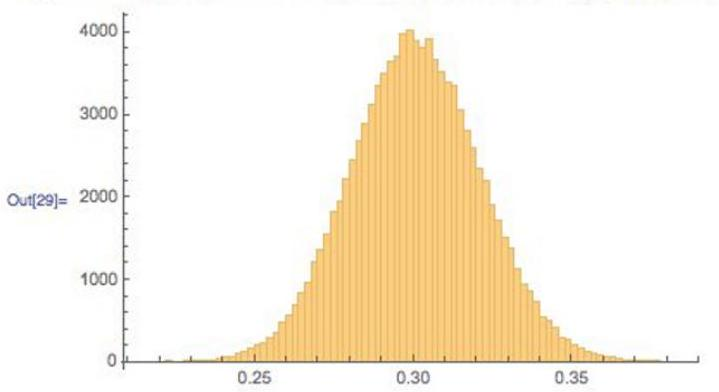
\includegraphics[max width=\textwidth]{2025_03_17_ca60ec0bfd96dcf8e028g-055}
  \caption{Sample \textenglish{variance} \textenglish{on} \textenglish{hitters} \textenglish{with} \textenglish{a} \textenglish{real} 30\% \textenglish{success} \textenglish{rate} \textenglish{results} \textenglish{in} \textenglish{a} \textenglish{wide} \textenglish{range} \textenglish{of} \textenglish{observed} \textenglish{performance} \textenglish{even} \textenglish{over} 500 \textenglish{trials} \textenglish{per} season.}
\end{figure}

चित्र 2.5 एक साधारण सिम्युलेशन के परिणामों को दर्शाता है, जहाँ 500 एट-बैट्स/सीज़न में प्रत्येक एट-बैट के परिणाम को तय करने के लिए यादृच्छिक संख्याओं का उपयोग किया गया था। हमारा सिंथेटिक खिलाड़ी वास्तव में .300 हिटर है, क्योंकि हमने इसे $300 / 1000$(0.3) की संभावना के साथ हिट रिपोर्ट करने के लिए प्रोग्राम किया है। परिणाम दिखाते हैं कि एक वास्तविक .300 हिटर के पास .275 या उससे कम हिट करने का 10\%मौका होता है, केवल संयोगवश। ऐसे सीज़न को आमतौर पर चोटों या संभवतः खिलाड़ी की उम्र के खेल प्रदर्शन पर अनिवार्य प्रभावों द्वारा समझाया जाता है। लेकिन यह सिर्फ प्राकृतिक बदलाव भी हो सकता है। समझदार टीमें एक खराब सीजन के बाद अच्छे हिटर को सस्ता खरीदने का प्रयास करती हैं, इस बदलाव का लाभ उठाने की कोशिश करती हैं।

हमारा .300 बल्लेबाज़ भी .325 से ऊपर बल्लेबाजी करने की 10% संभावना रखता है, लेकिन आप...

%---- \textenglish{Page} \textenglish{End} \textenglish{Break} \textenglish{Here} ---- \textenglish{Page} : 38

वे काफी हद तक यकीन के साथ कह सकते हैं कि वे ऐसे उत्कृष्ट सत्र को उनके बेहतर कंडिशनिंग या प्रशिक्षण विधियों को श्रेय देंगे, बजाय इसके कि वे केवल भाग्यशाली रहे। अच्छा या बुरा सत्र, या भाग्यशाली/अभाग्यशाली: संकेत को शोर से अलग करना मुश्किल होता है।

\begin{itemize}
  \item \textit{मॉडल प्रदर्शन}: डेटा वैज्ञानिकों के रूप में, हम आमतौर पर प्रत्येक भविष्यवाणी चुनौती के लिए कई मॉडलों का विकास और मूल्यांकन करेंगे। मॉडल बहुत सरल से लेकर जटिल तक हो सकते हैं, और उनके प्रशिक्षण शर्तों या पैरामीटर्स में भिन्नता हो सकती है।
\end{itemize}

आमतौर पर प्रशिक्षण कॉर्पस पर सबसे अच्छी सटीकता वाला मॉडल दुनियां के सामने सही मॉडल के रूप में गर्व से प्रदर्शित किया जाएगा। लेकिन मॉडलों के प्रदर्शन में छोटे-छोटे भिन्नताओं की व्याख्या साधारण विचरण के बजाय बुद्धिमत्ता से अधिक होती है: कौन से प्रशिक्षण/मूल्यांकन युग्म चुने गए, किस हद तक पैरामीटर अनुकूलित किए गए, आदि।\\
मशीन लर्निंग मॉडलों का प्रशिक्षण करते समय इसे याद रखें। वाकई, जब मॉडलों के बीच छोटे प्रदर्शन भिन्नताओं का चयन करने के लिए कहा जाता है, तो मैं सबसे सरल मॉडल के पक्ष में तर्क करने की संभावना अधिक रखता हूँ बजाय उस मॉडल के जो उच्चतम स्कोर लेता हो। एक ऐसे सौ लोगों के समूह में जिनके पास सिक्का उछालने के धारा पर सिर और पूंछ की पूर्वानुमान लगाने की कोशिश है, उनमें से एक को सबसे ज्यादा सही उत्तर पाने की गारंटी होगी। लेकिन यह विश्वास करने का कोई कारण नहीं है कि इस व्यक्ति के पास हम में से बाकी लोगों की तुलना में कोई बेहतर भविष्यवाणी शक्ति है।

\subsection{वितरणों की विशेषता}
वितरणों में आवश्यक रूप से बहुत अधिक संभावना द्रव्यमान ठीक औसत पर नहीं होता है। विचार करें कि आपका धन कैसा दिखेगा जब आप\$100 मिलियन उधार लेंगे, और फिर इसे एक समान मनी सिक्का उछाल पर दांव लगा देंगे। सिर आया तो अब आपके पास\$100 मिलियन साफ हैं, और पूंछ आया तो आप\$100 मिलियन कर्ज में। आपकी अपेक्षित संपत्ति शून्य है, लेकिन यह औसत आपको आपके धन वितरण के आकार के बारे में ज्यादा नहीं बताता है।\index{crowdsourcing}

हालांकि, औसत और मानक अंतरक \textenglish{together} एक \textit{किसी भी} वितरण को वर्णन करने में एक अच्छी भूमिका निभाते हैं। यहाँ तक कि अपेक्षाकृत थोड़ी मात्रा में द्रव्यमान अगर औसत से दूर स्थित होती है, तो यह मानक अंतरक में काफी बढ़ोतरी करेगी, इसलिए एक छोटी $\sigma$का अर्थ है कि अधिकतर द्रव्यमान औसत के पास होना चाहिए।

सटीक होने के लिए, चाहे आपका डेटा कैसे भी वितरित किया जाए, कम से कम$(1 - (1 / k^2))$वज़न का हिस्सा औसत के $k\pm मानक विचलनों के भीतर होना चाहिए। इसका अर्थ है कि सभी डेटा का कम से कम$75\%$औसत के$2$\sigma के भीतर होना चाहिए, और लगभग$89\%$किसी भी वितरण के लिए$3$\sigma के भीतर होना चाहिए।

हम देखेंगे कि जब हमें पता होता है कि वितरण अच्छी तरह से प्रस्तुत है, जैसे कि गॉसियन या सामान्य वितरण, तो और भी कड़ा बॉउंड हो सकता है। लेकिन यही कारण है कि औसत के बारे में बात करते समय दोनों$\mu$और$\sigma$को रिपोर्ट करना एक महान अभ्यास है। संयुक्त राज्य अमेरिका में वयस्क महिलाओं की औसत ऊँचाई $63.7\pm $2.7$ इंच है, जिसका अर्थ है\mu$=63.7$और\sigma$=2.7@। ऑरलैंडो, फ्लोरिडा में औसत तापमान 60.3 डिग्री फारेनहाइट है। हालांकि, डिज़्नी वर्ल्ड में 100 डिग्री दिन अधिक हुए हैं, जबकि 100 इंच (8.33 फुट) ऊँची महिलाएं उनका आनंद लेने के लिए आती हैं।

\textit{घर का पाठ}: अपने वितरण को वर्णित करने के लिए औसत और मानक विचलन दोनों की रिपोर्ट करें, लेखा के रूप में$\mu\pm\sigma$.\index{Darwin, Charles}\index{Galton, Francis}

\section{सहसंबंध विश्लेषण}
\index{social media!analysis}\index{coordination!analysis}मान लीजिए कि हमें दो चर$x$और$y$दिए गए हैं, जिन्हें$(x_{i}, y_{i})$रूप के$n$बिंदुओं के नमूने द्वारा दर्शाया गया है, जहाँ$1\leqi\leqn$होता है। हम कहते हैं कि$x$और$y$\textit{सहसंबंधित}हैं जब$x$का मान$y$के मान पर कुछ भविष्यवाणी शक्ति रखता है।\index{anchoring}\index{Surowiecki, James}

\textit{सहसंबंध गुणांक} $r(X, \textenglish{Y})$ एक सांख्यिकी है जो यह मापता है कि किस हद तक $Y$ $X$ का कार्य है, और इसके विपरीत। सहसंबंध गुणांक का मान -1 से 1 तक होता है, जहाँ 1 का अर्थ पूरी तरह से सहसंबद्धता और 0 का अर्थ कोई संबंध नहीं होता, या स्वतंत्र चर होते हैं। नकारात्मक सहसंबंध संकेत देते हैं कि चर \textit{विपरीत-संबंधित} होते हैं, जिसका अर्थ है कि जब $X$ बढ़ता है, $Y$ घटता है।

पूर्णतः प्रतिकूल सहसंबद्ध चर का सहसंबंध -1 होता है। ध्यान दें कि भविष्यवाणी के लिए नकारात्मक सहसंबंध सकारात्मक सहसंबंध के समान ही अच्छे होते हैं। अधिक शिक्षा से बेरोज़गार होने की संभावना कम होती है, यह नकारात्मक सहसंबंध का एक उदाहरण है, इसलिए शिक्षा का स्तर वास्तव में नौकरी की स्थिति की भविष्यवाणी करने में मदद कर सकता है। 0 के आसपास के सहसंबंध पूर्वानुमान के लिए बेकार होते हैं।

प्रेक्षित सहसंबंध उन भविष्यवाणी मॉडलों में महत्वपूर्ण भूमिका निभाते हैं जिन्हें हम डेटा विज्ञान में बनाते हैं। सहसंबंधों की प्रतिनिधि ताकत में शामिल हैं:

\begin{itemize}
  \item क्या लंबे लोग अधिक पतले रहने की संभावना रखते हैं? ऊँचाई और बीएमआई के बीच देखा गया सहसंबंध $r=-0.711$ है, इसलिए ऊँचाई का शरीर द्रव्यमान सूचकांक (बीएमआई) के साथ नकारात्मक संबंध है।\footnote{\url{https://onlinecourses.science.psu.edu/stat500/node/60}}
  \item क्या मानकीकृत परीक्षण कॉलेज में छात्रों के प्रदर्शन की भविष्यवाणी करते हैं? \textenglish{SAT} स्कोर और फ्रेशमेन \textenglish{GPA} के बीच देखा गया सहसंबंध $r=0.47$ है, इसलिए हाँ, कुछ हद तक भविष्यवाणी शक्ति है। लेकिन सामाजिक आर्थिक स्थिति भी \textenglish{SAT} स्कोर के साथ उतनी ही दृढ़ता से सहसंबंधित है $(r=0.42)$।\footnote{\url{https://research.collegeboard.org/sites/default/files/publications/2012/9/researchreport-2009-1-socioeconomic-status-sat-freshman-gpa-analysis-data.pdf}}
  \item क्या आर्थिक स्थिति स्वास्थ्य को प्रभावित करती है? घरेलू आय और कोरोनरी आर्टरी डिजीज के प्रसार के बीच देखा गया सहसंबंध $r=-0.717$ है, इसलिए एक मजबूत नकारात्मक सहसंबंध है। तो हाँ, जितने आप समृद्ध होंगे, दिल के दौरे का जोखिम उतना कम होगा।\footnote{\url{http://www.ncbi.nlm.nih.gov/pmc/articles/PMC3457990/}}
  \item क्या धूम्रपान स्वास्थ्य को प्रभावित करता है? एक समूह के धूम्रपान करने की प्रवृत्ति और उनकी मृत्यु दर के बीच देखा गया सहसंबंध $r=0.716$ है, इसलिए भगवान के लिए, धूम्रपान न करें।\footnote{\url{http://lib.stat.cmu.edu/DASL/Stories/SmokingandCancer.html}}
  \item क्या हिंसक वीडियो गेम आक्रामक व्यवहार को बढ़ाते हैं? खेल और हिंसा के बीच देखा गया सहसंबंध $r=0.19$ है, इसलिए एक कमजोर लेकिन महत्वपूर्ण सहसंबंध है।\footnote{\url{http://webspace.pugetsound.edu/facultypages/cjones/chidev/Paper/Articles/Anderson-Aggression.pdf}}\index{aggregation mechanisms}\index{Amazon Turk}\index{Amazon Turk!Turkers}\index{Arrow’s \textenglish{impossibility} theorem}\index{Condorcet \textenglish{jury} theorem}\index{CrowdFlower}\index{crowdsourcing services}\index{weighted average}
\end{itemize}

इस खंड में सहसम्बन्ध के प्राथमिक मापों का परिचय दिया जाएगा। आगे, हम यह अध्ययन करेंगे कि किसी भी देखे गए सहसम्बन्ध की शक्ति और क्षमता को उपयुक्त रूप से कैसे निर्धारित करें, ताकि हमें यह समझने में मदद मिल सके कि जब चर के बीच के संबंध वास्तविक होते हैं।

\subsection{सम्मिलन गुणांक: पीयरसन और स्पीयरमैन रैंक}
वास्तव में, सम्मिलन मापने के लिए दो मुख्य सांख्यिकी आंकड़े प्रयोग किए जाते हैं। सौभाग्य से, दोनों एक ही $-1$ से $1$ मापदंड पर कार्य करते हैं, हालांकि वे कुछ अलग चीजें मापते हैं। ये विभिन्न आंकड़े अलग-अलग परिस्थितियों में उपयुक्त होते हैं, इसलिए आपको इन दोनों के बारे में जानना चाहिए।

\subsection{पीयरसन कोरेलैशन कोएफिशिएंट}
दो आँकड़ों में प्रमुख पीयरसन कोरेलैशन है, जिसे इस प्रकार परिभाषित किया गया है:

\[r =\frac{\sum_{i=1}^{n}(X_{i}-\bar{X})(Y_{i}-\bar{Y})}{\sqrt{\sum_{i=1}^{n}(X_{i}-\bar{X})^{2}} \sqrt{\sum_{i=1}^{n}(Y_{i}-\bar{Y})^{2}}}=\frac{\operatorname{कोव}(X, \textenglish{Y})}{\sigma(\textenglish{X}) \sigma(\textenglish{Y})}\]

आइए इस समीकरण का विश्लेषण करें। मान लीजिए$X$और$Y$के बीच मजबूत संबंध है। तब हम उम्मीद करेंगे कि जब$x_{i}$उसके औसत$\bar{X}$से अधिक होगा, तो$y_{i}$अपने औसत$\bar{Y}$से बड़ा होना चाहिए। जब$x_{i}$अपने औसत से कम होता है,$y_{i}$को उसका अनुसरण करना चाहिए। अब अंश को देखें। जब दोनों मान$(1\times1)$से ऊपर या$(-1\times-1)$से नीचे होते हैं, तो प्रत्येक पद का चिह्न सकारात्मक होता है। यदि वे विपरीत दिशाओं में चलते हैं, तो प्रत्येक पद का चिह्न नकारात्मक$((-1\times1)$या$(1\times-1))$होता है, जो नकारात्मक सहसंबंध का संकेत देता है। यदि$X$और$Y$का कोई संबंध नहीं है, तो सकारात्मक और नकारात्मक पद समान आवृत्ति के साथ होनी चाहिए, एक-दूसरे को संतुलित करते हुए और मान को शून्य की ओर ले जाते हुए।

अंश का ऑपरेशन जो सहसंबंध के चिह्न को निर्धारित करता है, इतना उपयोगी है कि हम इसे एक नाम देते हैं, कोवेरियन्स, जिसकी गणना की जाती है:

\[\operatorname{कोव}(X, \textenglish{Y}) =\sum_{i=1}^{n}(X_{i}-\bar{X})(Y_{i}-\bar{Y})\]\index{machine learning!classifiers}

कावेariance याद रखें: हम इसे फिर से ⸨अनुभाग 8.2.3⸩ में देखेंगे।\\
\textenglish{Pearson} सूत्र का हरायक इन दो चरों में होने वाले परिवर्तन की मात्रा को दर्शाता है, जैसा कि उनके मानक विचलनों द्वारा मापा जाता है। $X$ और $Y$ के बीच सहप्रसरण इन चरों के परिवर्तन के साथ संभावित रूप से बढ़ता है, और यह हरायक जादुई मात्रा है जिसके द्वारा विभाजित करके सहसंबंध को $-1$ से $1$ के पैमाने पर लाया जाता है।\index{A/B testing}\index{CrowdFlower}\index{Emoji Dick}\index{Moby Dick}\index{Sheep Market}

%---- \textenglish{Page} \textenglish{End} \textenglish{Break} \textenglish{Here} ---- \textenglish{Page} : 41





\begin{figure}[h]
    \centering
    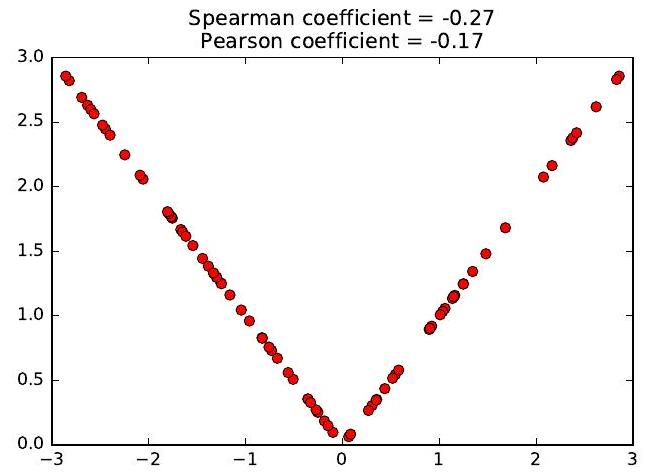
\includegraphics[max width=\textwidth]{2025_03_17_ca60ec0bfd96dcf8e028g-059}
    \caption{The \textenglish{function} $y=|x|$ \textenglish{does} \textenglish{not} \textenglish{have} \textenglish{a} \textenglish{linear} model, \textenglish{but} \textenglish{seems} \textenglish{like} \textenglish{it} \textenglish{should} \textenglish{be} \textenglish{easily} \textenglish{fitted} \textenglish{despite} \textenglish{weak} correlations.}
    \label{fig:abs-function}
\end{figure}

पीयरसन सम्बन्ध गुणांक यह परिभाषित करता है कि कौनसी सीमा तक $y=mx+b$ के रूप के एक रैखिक प्रेडिक्टर पर्यवेक्षित डेटा से मेल खा सकता है। यह सामान्यतः चरों के बीच समानता का माप करने में अच्छा काम करता है, लेकिन यह संभव है कि कुछ विशेष उदाहरणों का निर्माण किया जाए जहां $X$ और $Y$ के बीच का सम्बन्ध गुणांक शून्य हो, फिर भी $Y$ पूरी तरह से $X$ पर निर्भर हो (और इस प्रकार @X@ से पूरी तरह पूर्वानुमेय हो)।

विचार करें बिंदुओं के रूप $(x,|x|)$ पर, जहां $x$ का समान रूप से (या सममित रूप से) नमूनाकरण $[-1,1]$ अंतराल से किया जाता है जैसा कि चित्र \ref{चित्र:abs-функ्शन} में दिखाया गया है। सहसंबंध शून्य होगा क्योंकि हर बिंदु $(x, \textenglish{x})$ के लिए एक विपरीत बिंदु $(-x, \textenglish{x})$ होगा, फिर भी $y=|x|$ एक उत्तम भविष्यवक्ता है। पीयरसन सहसंबंध मापता है कि उत्तम रैखिक भविष्यवक्ता कितनी अच्छी तरह काम कर सकते हैं, लेकिन यह अजीब कार्यों जैसे कि पार पूर्ण मूल्य के बारे में कुछ नहीं कहता है।

स्पीयरमैन रैंक सहसंबंध गुणांक मुख्यतः इनपुट बिंदुओं की जोड़ों की संख्या गिनता है जो बिना क्रम के हैं। मान लीजिए कि हमारे डेटा सेट में बिंदु$\left(x_{1}, y_{1}\right)$और$\left(x_{2}, y_{2}\right)$होते हैं जहाँ$x_{1}< x_{2}$और$y_{1}< y_{2}$। यह एक मत है कि मान सकारात्मक रूप से सहसंबंधित हैं, जबकि मत नकारात्मक सहसंबंध के लिए होगा यदि$y_{2}< y_{1}$।

सभी बिंदुओं के जोड़ों पर जोड़कर और उचित रूप से सामान्यीकरण करके हमें स्पीयर्समैन रैंक सहसंबंध प्राप्त होता है। \operatorname{rank} में${x_{i}\leftका रैंक स्थान बिक्री क्रम में सभी {x_⸨i}\rightमें से होगा, इसलिए सबसे छोटे मान का रैंक 1 होगा और सबसे बड़े मान का$n$। तब

\[
\rho=1-\frac{6 \sum d_{i}^{2}}{n\left(n^{2}-1\right)}
\]

where$d_{i}=\operatorname{स्थान}\left(x_{i}\right)-\operatorname{स्थान}\left(y_{i}\right)$.

\begin{figure}[h]
    \centering
    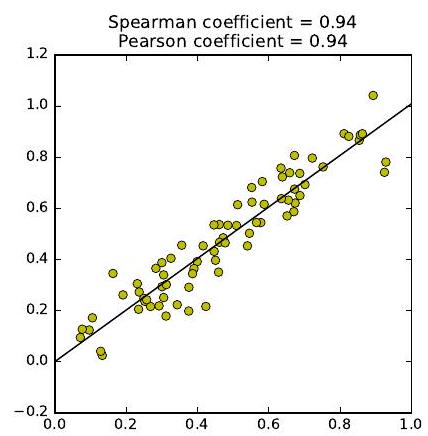
\includegraphics[max width=\textwidth]{2025_03_17_ca60ec0bfd96dcf8e028g-060}
    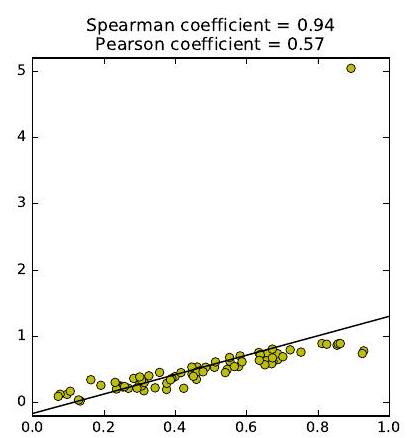
\includegraphics[max width=\textwidth]{2025_03_17_ca60ec0bfd96dcf8e028g-060(1)}
    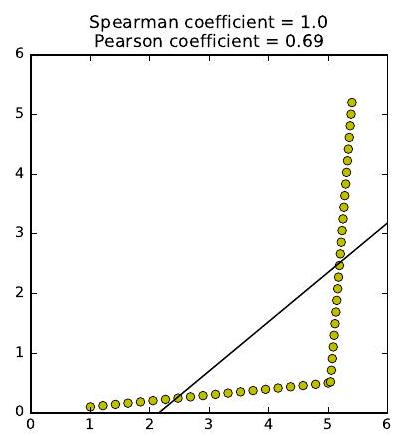
\includegraphics[max width=\textwidth]{2025_03_17_ca60ec0bfd96dcf8e028g-060(2)}
    \caption{A \textenglish{monotonic} \textenglish{but} \textenglish{not} \textenglish{linear} \textenglish{point} \textenglish{set} \textenglish{has} \textenglish{a} \textenglish{Spearman} \textenglish{coefficient} $r=1$ \textenglish{even} \textenglish{though} \textenglish{it} \textenglish{has} \textenglish{no} \textenglish{good} \textenglish{linear} \textenglish{fit} (\textenglish{left}). Highly-correlated \textenglish{sequences} \textenglish{are} \textenglish{recognized} \textenglish{by} \textenglish{both} \textenglish{coefficients} (\textenglish{center}), \textenglish{but} \textenglish{the} \textenglish{Pearson} \textenglish{coefficient} \textenglish{is} \textenglish{much} \textenglish{more} \textenglish{sensitive} \textenglish{to} \textenglish{outliers} (\textenglish{right}).}\index{games \textenglish{with} \textenglish{a} purpose}\index{gamification}\index{institutional \textenglish{review} board}
    \label{fig:spearman-pearson}
\end{figure}

गैर-रेखीय लेकिन मोनोटोनिक फंक्शन्स को उच्च स्कोर देने के अलावा, स्पीयरमैन सहसंबंध पियर्सन की तुलना में अत्यधिक अपवाद तत्वों के प्रति कम संवेदनशील होता है। मान लीजिए$p=(x_{1}, y_{\max})$वह डेटा पॉइंट है जिसका$y$के लिए दिए गए डेटा सेट में सबसे बड़ा मान है। मान लें कि हम$p$को$p'=(x_{1},\infty)$से बदलते हैं। पियर्सन सहसंबंध पागल हो जाएगा, क्योंकि अब सर्वश्रेष्ठ फिट ऊर्ध्वाधर रेखा$x=x_{1}$बन जाती है। लेकिन स्पीयरमैन सहसंबंध अपरिवर्तित रहेगा, क्योंकि सभी बिंदु$p$के तहत थे, जैसे कि वे अब$p'$के तहत हैं।

\subsection{संगति की शक्ति और महत्व}

सह-संबंध गुणांक$r$इस बात को दर्शाता है कि किस हद तक$x$का उपयोग किसी दिए गए बिंदु के नमूने$S$में$y$को भविष्यवाणी करने के लिए किया जा सकता है। जैसे-जैसे$|r|\rightarrow1$होता है, ये भविष्यवाणियाँ बेहतर और बेहतर होती जाती हैं।

लेकिन असली सवाल यह है कि नमूने के बाहर, वास्तविक दुनिया में यह संबंध कैसे बना रहेगा। मजबूत संबंधों का $|r|$ बड़ा होता है, लेकिन वे काफी बिंदुओं के नमूनों के साथ जुड़ा होता है जिससे वे महत्वपूर्ण हो जाते हैं। एक व्यंग्यात्मक कहावत है कि अगर आप अपने डेटा को सीधी रेखा से फिट करना चाहते हैं, तो इसे केवल दो बिंदुओं पर नमूनांकित करना सबसे अच्छा होता है। आपका संबंध जितने अधिक बिंदुओं पर आधारित होता है, उतना ही प्रभावशाली लगता है।

सांख्यिकीय सीमाओं को परस्पर संबन्धों के व्याख्या में प्रस्तुत किया गया है चित्र\ref{fig:correlation-limits}में, जो शक्ति और आकार पर आधारित हैं:

\begin{itemize}
  \item \textbf{Strength \textenglish{of} correlation: $R^{2}$ :} \textenglish{The} \textenglish{square} \textenglish{of} \textenglish{the} \textenglish{sample} \textenglish{correlation} \textenglish{coefficient} $r^{2}$ \textenglish{estimates} \textenglish{the} \textenglish{fraction} \textenglish{of} \textenglish{the} \textenglish{variance} \textenglish{in} $Y$ \textenglish{explained} \textenglish{by} $X$ \textenglish{in} \textenglish{a} \textenglish{simple} \textenglish{linear} regression. \textenglish{The} \textenglish{correlation} \textenglish{between} \textenglish{height} \textenglish{and} \textenglish{weight} \textenglish{is} \textenglish{approximately} 0.8, \textenglish{meaning} \textenglish{it} \textenglish{explains} \textenglish{about} two-thirds \textenglish{of} \textenglish{the} variance.
  
  \begin{figure}[h]
      \centering
      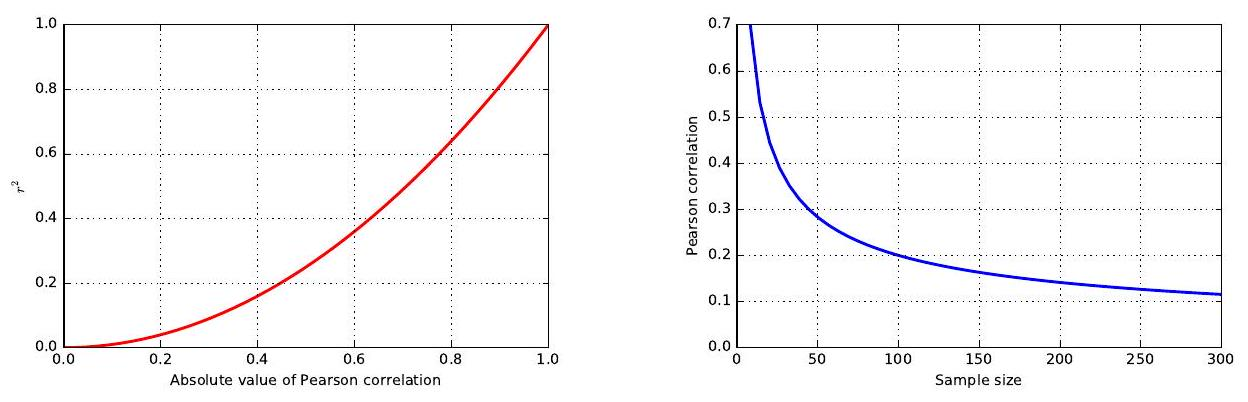
\includegraphics[max width=\textwidth]{2025_03_17_ca60ec0bfd96dcf8e028g-061(1)}
      \caption{Limits \textenglish{in} \textenglish{interpreting} significance. \textenglish{The} $r^{2}$ \textenglish{value} \textenglish{shows} \textenglish{that} \textenglish{weak} \textenglish{correlations} \textenglish{explain} \textenglish{only} \textenglish{a} \textenglish{small} \textenglish{fraction} \textenglish{of} \textenglish{the} \textenglish{variance} (\textenglish{left}). \textenglish{The} \textenglish{level} \textenglish{of} \textenglish{correlation} \textenglish{necessary} \textenglish{to} \textenglish{be} \textenglish{statistically} \textenglish{significant} \textenglish{decreases} \textenglish{rapidly} \textenglish{with} \textenglish{sample} \textenglish{size} $n$ (\textenglish{right}).}
      \label{fig:correlation-limits}
  \end{figure}
  
  \textenglish{Figure} \ref{fig:correlation-limits} (\textenglish{left}) \textenglish{shows} \textenglish{how} \textenglish{rapidly} $r^{2}$ \textenglish{decreases} \textenglish{with} $r$. \textenglish{There} \textenglish{is} \textenglish{a} \textenglish{profound} \textenglish{limit} \textenglish{to} \textenglish{how} \textenglish{excited} \textenglish{we} \textenglish{should} \textenglish{get} \textenglish{about} \textenglish{establishing} \textenglish{a} \textenglish{weak} correlation. \textenglish{A} \textenglish{correlation} \textenglish{of} 0.5 \textenglish{possesses} \textenglish{only} 25\% \textenglish{of} \textenglish{the} \textenglish{maximum} \textenglish{predictive} power, \textenglish{and} \textenglish{a} \textenglish{correlation} \textenglish{of} $r=0.1$ \textenglish{only} 1\%. Thus, \textenglish{the} \textenglish{predictive} \textenglish{value} \textenglish{of} \textenglish{correlations} \textenglish{decreases} \textenglish{rapidly} \textenglish{with} $r$.
\end{itemize}

हम "वैरिएन्स को समझाने" से क्या मतलब रखते हैं? मान लें कि $f(\textenglish{x})=mx+c$ एक भविष्यवाणी मान है, जो $y$ को $x$ से जोड़ता है, जहां पैरामीटर्स $m$ और $c$ सबसे अच्छे संभावित फिट के अनुरूप होते हैं। अवशिष्ट मान $r_{i}=y_{i}-f\left(x_{i}\right)$ का औसत शून्य होगा, जैसा कि चित्र \ref{fig:residuals} में दिखाया गया है। इसके अलावा, यदि $f(\textenglish{x})$ के लिए एक अच्छा रैखिक फिट है, तो पूर्ण डेटा सेट $V(\textenglish{Y})$ का वैरिएन्स $V(\textenglish{r})$ से कहीं अधिक होना चाहिए। यदि $x$ और $y$ पूरी तरह से सम्बन्धित हैं, तो कोई अवशिष्ट त्रुटि नहीं होनी चाहिए, और $V(\textenglish{r})=0$ होगा। यदि $x$ और $y$ पूरी तरह से असम्बद्ध हैं, तो फिट को कुछ भी योगदान नहीं देना चाहिए, और $V(\textenglish{y})\approx लगभग $V(\textenglish{r})$ होगा। सामान्य तौर पर, $1-r^{2}=V(\textenglish{r}) / V(\textenglish{y})@।\index{Babbage, Charles}\index{exercises}

\begin{figure}[h]
    \centering
    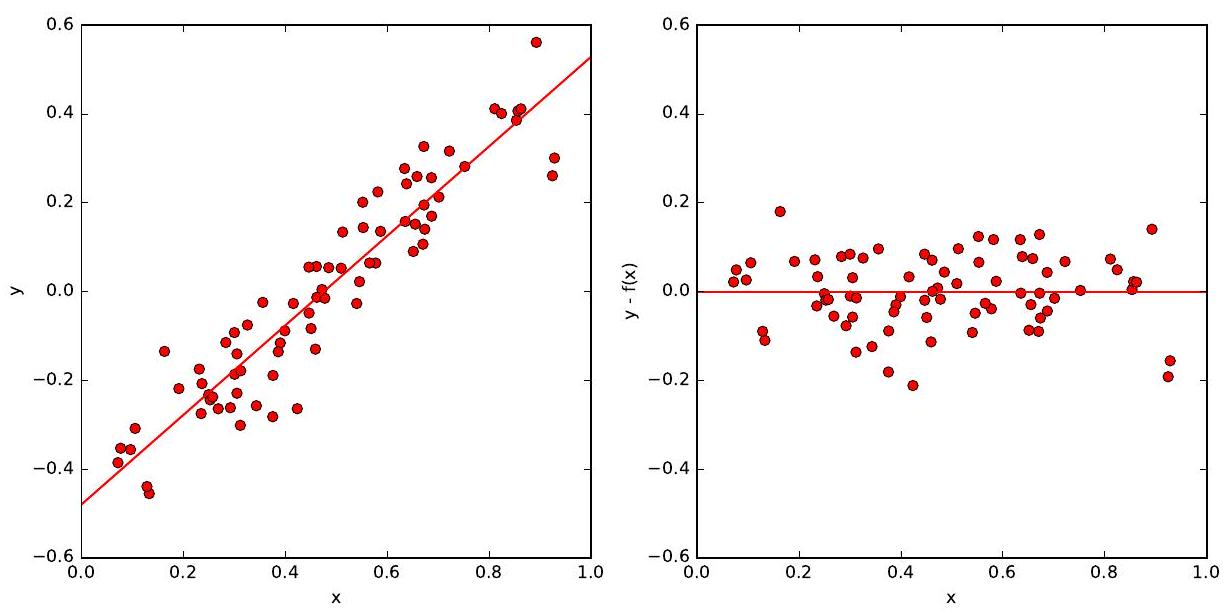
\includegraphics[max width=\textwidth]{2025_03_17_ca60ec0bfd96dcf8e028g-061}
    \caption{Plotting $r_{i}=y_{i}-f\left(x_{i}\right)$ \textenglish{shows} \textenglish{that} \textenglish{the} \textenglish{residual} \textenglish{values} \textenglish{have} \textenglish{lower} \textenglish{variance} \textenglish{and} \textenglish{mean} zero. \textenglish{The} \textenglish{original} \textenglish{data} \textenglish{points} \textenglish{are} \textenglish{on} \textenglish{the} left, \textenglish{with} \textenglish{the} \textenglish{corresponding} \textenglish{residuals} \textenglish{on} \textenglish{the} right.}
    \label{fig:residuals}
\end{figure}

विचार करें चित्र\ref{fig:residuals}, जिसमें बिंदुओं का एक सेट (बाएँ) चित्रित है जो एक अच्छा रैखिक मिलान प्रकट करता है, जिसका सहसंबंध$r=0.94$ है। संबंधित अवशेष$r_{i}=y_{i}-f\left(x_{i}\right)$ दाएँ ओर प्रदर्शित हैं। बाएँ पर$y$ मानों का विचलन$V(\textenglish{y})=0.056$, दाएँ पर विचलन$V(\textenglish{r})=0.0065$ से काफी अधिक है। वास्तव में,

\[
1-r^{2}=0.116 \longleftrightarrow V(\textenglish{r}) / V(\textenglish{y})=0.116
\]

\begin{itemize}
  \item \textbf{सांख्यिकीय महत्व:} एक सहसंबंध का सांख्यिकीय महत्व इसके नमूना आकार $n$ के साथ-साथ $r$ पर निर्भर करता है। परंपरा के अनुसार, हम कहते हैं कि $n$ बिंदुओं का सहसंबंध महत्वपूर्ण है यदि $\alpha\leq $ 1 / 20=0.05$ संभावना है कि हम किसी भी यादृच्छिक सेट $n$ बिंदुओं में $r$ जितना मजबूत सहसंबंध देखेंगे।
  
  यह विशेष रूप से मजबूत मानक नहीं है। बड़े नमूना आकारों के साथ छोटे सहसंबंध भी 0.05 स्तर पर महत्वपूर्ण हो जाते हैं, जैसा कि चित्र \ref{fig:correlation-limits} (दाईं ओर) में दिखाया गया है। $r=0.1$ का सहसंबंध \alpha$$= 0.05$ के आसपास @n=300@ पर महत्वपूर्ण हो जाता है, भले ही ऐसा कारक केवल 1\% विचलन को समझाता हो।
\end{itemize}

कमजोर लेकिन महत्वपूर्ण सहसंबंध बड़े डाटा मॉडल में मूल्यवान हो सकते हैं, जिनमें बड़ी संख्या में विशेषताएँ शामिल होती हैं। कोई भी एकल विशेषता/सहसंबंध केवल छोटे प्रभावों को समझा/भविष्यवाणी कर सकता है, लेकिन एक साथ मिलकर कमजोर लेकिन स्वतंत्र सहसंबंधों की बड़ी संख्या में मजबूत भविष्यवाणी करने की क्षमता हो सकती है। शायद। हम खंड 5.3 में फिर से अधिक विस्तार से महत्व पर चर्चा करेंगे।

\subsection{संबंधन का अर्थ कारण नहीं होता!}
आपने इसे पहले सुना होगा: संबंधन का अर्थ कारण नहीं होता:

\begin{itemize}
  \item एक कब्जे में सक्रिय पुलिस की संख्या स्थानीय अपराध दर के साथ मजबूत रूप से संबंधित होती है, लेकिन पुलिस अपराध का कारण नहीं बनती।
  \item लोग जो दवा लेते हैं उसकी मात्रा इस संभावना से संबंधित होती है कि वे बीमार हैं, लेकिन दवा बीमारी का कारण नहीं बनती।
\end{itemize}

सर्वोत्तम स्थिति में, संकेत केवल एक दिशा में काम करता है। लेकिन कई देखे गए संबंध पूरी तरह से नकली होते हैं, जिसमें न तो किसी चर का दूसरे पर कोई वास्तविक प्रभाव होता है।

फिर भी,\textit{सहसंबंध कारण का संकेत देता है}सोच में एक सामान्य त्रुटि है, यहाँ तक कि उन लोगों के बीच भी जो तार्किक तर्क को समझते हैं। आमतौर पर कहें तो कुछ सांख्यिकीय उपकरण उपलब्ध होते हैं यह पता लगाने के लिए कि क्या वास्तव में$A$का$B$पर प्रभाव है। हम नियंत्रित प्रयोग कर सकते हैं, अगर हम एक चर में परिवर्तन कर सकते हैं और दूसरे पर उसका प्रभाव देख सकते हैं। उदाहरण के लिए, यह तथ्य कि हम लोगों को ऐसी डाइट पर रख सकते हैं जो उन्हें वजन कम करने पर मजबूर करती है बिना लम्बाई को कम किए, यह प्रबल साक्ष्य है कि वजन ऊँचाई का कारण नहीं होता। लेकिन अक्सर इन प्रयोगों को विपरीत तरीके से करना कठिन होता है, जैसे कि लोगों को छोटा करने का कोई तार्किक तरीका नहीं है सिवाय उनके अंग काटने के।

\begin{figure}[h]
    \centering
    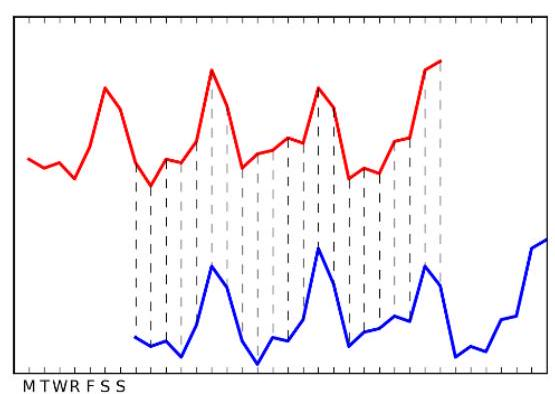
\includegraphics[max width=\textwidth]{2025_03_17_ca60ec0bfd96dcf8e028g-063}
    \caption{Correlation \textenglish{does} \textenglish{not} \textenglish{imply} causation. (\textenglish{Source} \href{https://www.xkcd.com/552}{https://www.xkcd.com/552})}
    \label{fig:correlation-causation}
\end{figure}

\begin{figure}[h]
    \centering
    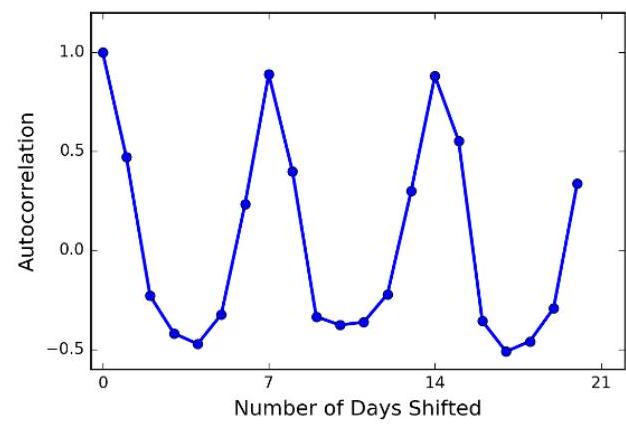
\includegraphics[max width=\textwidth]{2025_03_17_ca60ec0bfd96dcf8e028g-063(1)}
    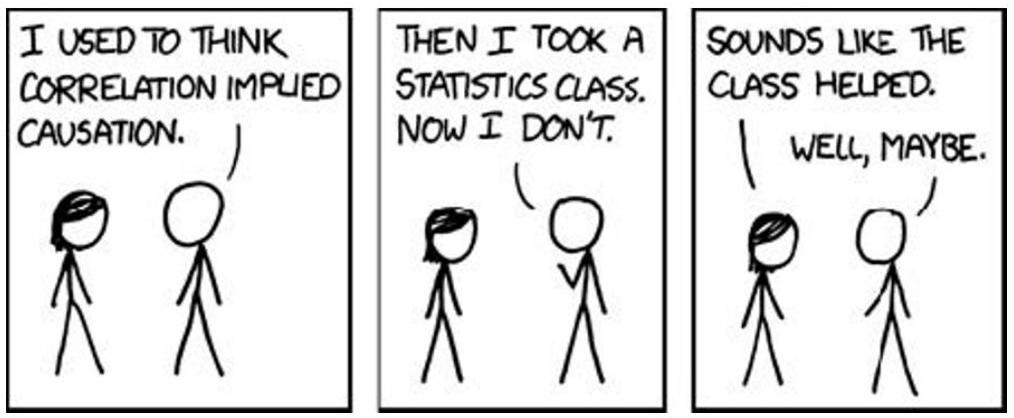
\includegraphics[max width=\textwidth]{2025_03_17_ca60ec0bfd96dcf8e028g-063(2)}
    \caption{Cyclic \textenglish{trends} \textenglish{in} \textenglish{a} \textenglish{time} \textenglish{series} (\textenglish{left}) \textenglish{are} \textenglish{revealed} \textenglish{through} \textenglish{correlating} \textenglish{it} \textenglish{against} \textenglish{shifts} \textenglish{of} \textenglish{itself} (\textenglish{right}).}
    \label{fig:cyclic-trends}
\end{figure}

\subsection{ऑटोकॉरलेशन द्वारा आवधिकता का पता लगाना}
मान लीजिए कोई अंतरिक्ष एलियन खिलौना कंपनी में अमरीकी बिक्री का विश्लेषण करने के लिए नियुक्त किया गया था। एक स्थिर प्रवृत्ति दिखाने वाले सुगम फ़ंक्शन के बजाय, उन्हें हर वर्ष बारहवें महीने में एक विशाल उछाल दिखकर आश्चर्य होगा। इस एलियन ने क्रिसमस के परिघटना की खोज की होती।

मौसमी प्रवृत्तियाँ एक निर्दिष्ट अवधि के चक्र को प्रतिबिंबित करती हैं, नियमित पैटर्न में ऊपर उठती और गिरती हैं। कई मानव गतिविधियाँ कार्य सप्ताह से संबंधित सात-दिवसीय चक्र के साथ आगे बढ़ती हैं। एक प्रकार के कीट की बड़ी आबादी, जिन्हें \textit{सिसाडा} कहा जाता है, 13-वर्षीय या 17-वर्षीय चक्र में उभरती हैं, ताकि शिकारी उन्हें सीख न सकें कि\
%---- पृष्ठ समाप्ति अवकाश यहाँ ---- पृष्ठ : 46

कैसे हम एक क्रम$S$में ऐसे चक्रीय पैटर्न पहचान सकते हैं? मान लीजिए हम$S_i$को$S_{i+p}$के साथ सभी$1\leqi\leqn-p$के लिए सह-संबंधित करते हैं। यदि किसी विशेष अवधि लंबाई$p$के लिए मान समकालिक हैं, तो अन्य संभावित अंतराल मूल्यों की तुलना में यह संबंध अपने आप में असामान्य रूप से उच्च होगा। एक क्रम की उसके साथ तुलना करना\textit{स्वतःसहसंबंध}कहलाता है, और सभी$1\leqk\leqn-1$के लिए संबंधों की श्रृंखला को\textit{स्वतःसहसंबंध फ़ंक्शन}कहा जाता है। चित्र 2.11 में दैनिक बिक्री की एक समय श्रृंखला और इस डेटा के लिए संबंधित स्वतःसहसंबंध फ़ंक्शन प्रस्तुत किया गया है। सात दिनों के शिफ्ट (और सात दिनों के हर गुणक) पर चोटी यह स्थापित करती है कि बिक्री में साप्ताहिक आवधिकता है: सप्ताहांत में अधिक सामान बिकता है।

ऑटोकॉरिलेशन भविष्य की घटनाओं की भविष्यवाणी करने में एक महत्वपूर्ण अवधारणा है, क्योंकि इसका अर्थ है कि हम किसी मॉडल में पूर्व के अवलोकनों को विशेषताओं के रूप में उपयोग कर सकते हैं। यह अनुमान कि कल का मौसम आज के समान होगा, ऑटोकॉरिलेशन पर आधारित है, जिसमें विलंब $p=1$दिन का होता है। निश्चित रूप से, हम उम्मीद करेंगे कि इस प्रकार का मॉडल छह महीने पुराने मौसम डेटा (विलंब $p=180$दिन) के आधार पर की गई भविष्यवाणियों से अधिक सटीक होगा।

सामान्यतः, कई मात्राओं के लिए स्वतःसंबंध कार्य सामान्यतः बहुत छोटे अन्तरालों के लिए सबसे उच्च होता है। यही कारण है कि दीर्घकालिक भविष्यवाणियाँ अल्पकालिक पूर्वानुमानों की तुलना में कम सटीक होती हैं: स्वतःसंबंध सामान्यतः बहुत कमजोर होते हैं। लेकिन आवधिक चक्र कभी-कभी बहुत लंबे खिंच जाते हैं। वास्तव में, $प=365$ दिनों के अन्तराल पर आधारित मौसम पूर्वानुमान $प=180$ के मुकाबले बेहतर होगा, मौसमी प्रभावों के कारण।

सम्पूर्ण स्वयंसंबंधन फलन की गणना करने के लिए समय श्रृंखला के अंक पर अलग-अलग संबंधों की$n-1$गणना करना आवश्यक होता है, जो बड़े$n$के लिए महँगा हो सकता है। सौभाग्य से, एक कुशल एल्गोरिदम है जो\textit{तेज फोरियर परिवर्तन}(\textenglish{FFT}) पर आधारित है, जो बहुत लंबे अनुक्रमों के लिए भी स्वयंसंबंधन फलन का निर्माण संभव बनाता है।

\section{लघुगणक}
\textit{लघुगणक} प्रत्यावर्ती घातांक फलन है$y = b^{x}$, यह एक समीकरण है जिसे इस प्रकार लिखा जा सकता है$x =\log_{b}y$। यह परिभाषा यह कहने के समान है कि

$$
b^{\log_{b} y}= y.
$$

घातीय फलन बहुत तेज़ गति से बढ़ते हैं: कल्पना करें {2^1, 2^2, 2^3, 2^4,}। इसके विपरीत, लघुगणक बहुत धीमी गति से बढ़ते हैं: ये केवल पिछली शृंखला के घातांक हैं {1, 2, 3, 4,}। इनका संबंध किसी भी प्रक्रिया से होता है जहां हम$b\ldots को बार-बार किसी मान से गुणा कर रहे हैं, या$b$ से बार-बार भाग कर रहे हैं। बस परिभाषा याद रखें:

$$
\textenglish{y} =\log_{ख}x\longleftrightarrowb^{y}= \textenglish{x}
$$

लघुगणक बहुत उपयोगी चीज़ें हैं, और डेटा विश्लेषण में अक्सर उभरते हैं। यहाँ मैं डेटा विज्ञान में तीन महत्वपूर्ण भूमिकाएँ बताता हूँ जो लघुगणक निभाते हैं। आश्चर्यजनक रूप से, उनमें से केवल एक ही उन सात एल्गोरिदमिक अनुप्रयोगों से संबंधित है जो मैंने\textit{द एल्गोरिदम डिज़ाइन मैन्युअल}[Ski08] में प्रस्तुत किए हैं। वास्तव में, लघुगणक बहुत उपयोगी चीज़ें हैं।\index{American \textenglish{basketball} players}\index{football!American players}

\subsection{लघुगणक और संभावनाओं का गुणन}
\index{multiplying probabilities}लघुगणक पहली बार गणना में सहायता के रूप में आविष्कार किए गए थे, गुणा की समस्या को जोड़ की समस्या में बदलकर। विशेष रूप से, उत्पाद के लिए गणना करने के लिए$p = x\cdoty$, हम लघुगणकों के योग की गणना कर सकते हैं$s =\log_{b}x +\log_{b}y$और फिर लघुगणक का प्रतिलोम (अर्थात्$b$को$s$वीं घात तक बढ़ाकर) लेना होगा ताकि हमें$p$मिल सके, क्योंकि:\index{scatter plots}

$$
\textenglish{p} = x\cdoty = b^{\left(\log_{b} \textenglish{x} + \log_{b} y\right)}.
$$

यह वह तरकीब है जिसने यांत्रिक स्लाइड रूल्स को संचालित किया, जो जेब में आने वाले कैलकुलेटरों से पहले के ज़माने में गीक्स द्वारा उपयोग की जाती थी।

हालाँकि, यह विचार आज भी महत्वपूर्ण बना हुआ है, विशेष रूप से जब संभाव्यताओं की लंबी श्रृंखलाओं को गुणा किया जाता है। संभाव्यताएँ छोटे संख्या होती हैं। इस प्रकार, संभाव्यताओं की लंबी श्रृंखलाओं का गुणा बहुत छोटे संख्या उत्पन्न करता है जो बहुत दुर्लभ घटनाओं की संभावनाओं को नियंत्रित करता है। असली कंप्यूटरों पर फ्लोटिंग प्वाइंट गुणा के साथ गंभीर संख्यात्मक स्थिरता समस्याएँ होती हैं। संख्यात्मक त्रुटियाँ धीरे-धीरे सटीक संख्या में समाहित हो जाएँगी और अंततः छोटी संख्या के सच्चे मान को प्रबल कर देंगी।

संभावनाओं के लॉगरिदम को जोड़ना उन्हें गुणा करने की तुलना में संख्यात्मक रूप से अधिक स्थिर है, लेकिन यह एक समान परिणाम देता है क्योंकि:

$$
\prod_{i=1}^{n}p_{i}= b^{P},\text{ जहाँ }P =\sum_{i=1}^{n}\log_{b}(p_{i})
$$

हम अपनी योगफल को घातांक में बढ़ा सकते हैं अगर हमें वास्तविक प्रायिकता की आवश्यकता हो, लेकिन आमतौर पर यह आवश्यक नहीं होता। जब हमें बस दो प्रायिकताओं की तुलना करनी होती है यह निर्णय करने के लिए कि कौन सी बड़ी है, तो हम सुरक्षित रूप से लॉग दुनिया में रह सकते हैं, क्योंकि बड़े लॉगरिदम बड़ी प्रायिकताओं के अनुरूप होते हैं।

एक बात को समझना महत्वपूर्ण है। याद रखें कि$\log_{2}\left(\frac{1}{2}\right) = -1$। संभावनाओं के लॉग सभी ऋणात्मक संख्याएँ होती हैं, सिवाय$\log(1) = 0$ के। यही कारण है कि संभावनाओं के लॉग वाले समीकरणों में अक्सर अजीब जगहों पर ऋणात्मक संकेत होते हैं। इन्हें ध्यानपूर्वक देखिए।

\subsection{लघुगणक और अनुपात}
\index{ratio}\textit{अनुपात} उस रूप के मात्राएँ हैं $a / b$। वे अक्सर डेटा सेट में घटक विशेषताओं या विशेषता युग्मों से प्राप्त मानों के रूप में उत्पन्न होते हैं। विस्थापन डेटा को सामान्यीकृत करने के दौरान या समय के लिए अनुपात स्वाभाविक रूप से उत्पन्न होते हैं (जैसे कुछ उपचार के बाद का वजन प्रारंभिक वजन पर) या समय (जैसे आज की कीमत कल की कीमत पर)।

लेकिन अनुपात बढ़ने पर और घटने पर अलग-अलग तरह से व्यवहार करता है। ⸨रातियो$200 / 100$⸩ बुनियादी स्तर से ⸨200\%$⸩ ऊपर है, लेकिन ⸨100 / 200$⸩ के बावजूद केवल ⸨50\%$⸩ नीचे है। इस प्रकार अनुपातों का औसत लेना सांख्यिकीय गलती करना है। क्या आप वास्तव में चाहते हैं कि दुगुने और आधे होने का औसत बढ़ौत्तरी दर्शाए, बजाय इसके कि यह निरपेक्ष परिवर्तन के रूप में सामने आए?

%---- \textenglish{Page} \textenglish{End} \textenglish{Break} \textenglish{Here} ---- \textenglish{Page} : 48

% Mismatched: \chaptername{Logarithms}

\begin{figure}[h]
    \centering
    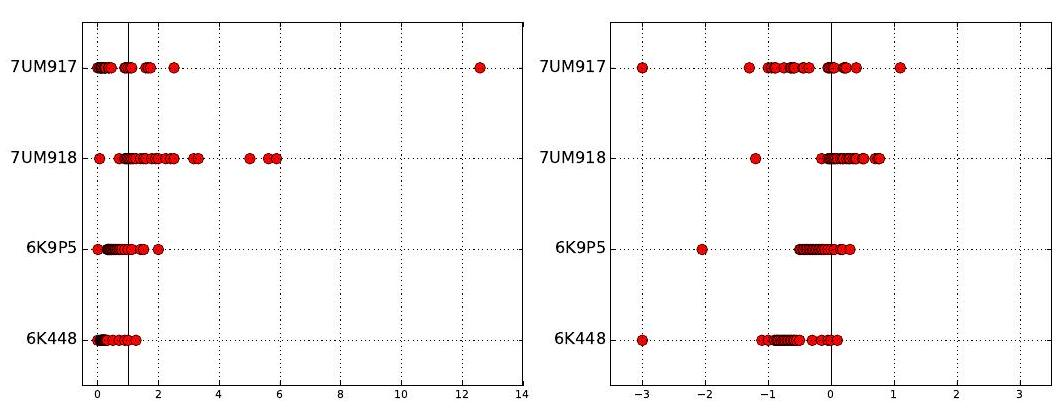
\includegraphics[max width=\textwidth]{2025_03_17_ca60ec0bfd96dcf8e028g-066}
    \caption{Plotting \textenglish{ratios} \textenglish{on} \textenglish{a} \textenglish{scale} \textenglish{cramps} \textenglish{the} \textenglish{space} \textenglish{allocated} \textenglish{to} \textenglish{small} \textenglish{ratios} \textenglish{relative} \textenglish{to} \textenglish{large} \textenglish{ratios} (\textenglish{left}). \textenglish{Plotting} \textenglish{the} \textenglish{logarithms} \textenglish{of} \textenglish{ratios} \textenglish{better} \textenglish{represents} \textenglish{the} \textenglish{underlying} \textenglish{data} (\textenglish{right}).}
\end{figure}

यहाँ एक समाधान ज्यामितीय माध्य का उपयोग करना हो सकता था। लेकिन इससे बेहतर है कि इन अनुपातों का लघुगणक लिया जाए, जिससे वे समान विस्थापन प्रदान करें, क्योंकि$\log_{2}2=1$और$\log_{2}(1 / 2)=-1$। हमें अतिरिक्त लाभ यह मिलता है कि एक इकाई अनुपात शून्य पर मैप होता है, जिससे सकारात्मक और नकारात्मक संख्या क्रमशः अनुचित और उचित अनुपातों के अनुरूप होते हैं।

मेरे छात्रों द्वारा अक्सर की जाने वाली एक शुरुआती गलती में अनुपातों के मूल्य की तुलना में उनके लगारिदमों का प्लॉट करना शामिल होता है। चित्र 2.12 (बाएँ) एक छात्र पत्र से लिया गया ग्राफ़ है, जो 24 घंटों के डाटा पर नए स्कोर के पुराने स्कोर के अनुपात को दिखाता है (प्रत्येक लाल बिंदु एक घंटे का माप है) चार अलग-अलग डाटा सेट्स पर (प्रत्येक को एक पंक्ति में दर्शाया गया है)। ठोस काली रेखा एक के अनुपात को दिखाती है, जहाँ दोनों स्कोर समान परिणाम देते हैं। अब इस ग्राफ़ को पढ़ने का प्रयास करें: यह आसान नहीं है क्योंकि रेखा के बाएँ ओर के बिंदु संकीर्ण पट्टी में संकुचित हैं। जो चीज़ आपके ध्यान में आती है वह हैं विसंगतियाँ। निश्चित रूप से नया एल्गोरिदम शीर्ष पंक्ति में 7UM917 पर भयानक प्रदर्शन करता है: दाएँ ओर सभी तरह का वह बिंदु एक वास्तविक विसंगति है।\index{bell-shaped!distribution}\index{good \textenglish{scoring} functions}\index{PageRank}\index{random variable!class rank}\index{random variable!search results}\index{random variable!top \textenglish{sports} teams}\index{random variable!university rankings}\index{scores vs. rankings}

हालांकि यह नहीं है। अब आकृति 2.12 (दाईं ओर) पर ध्यान दें, जहाँ हमने अनुपातों के लघुगणक का आलेख बनाया है। काले रेखा के बाईं और दाईं ओर के स्थान को अब बराबर किया जा सकता है। और यह दर्शाता है कि यह बिंदु वास्तव में ऐसा बाहरी नहीं था। बाईं ओर के बिंदुओं का सुधार का परिमाण दाईं ओर के बिंदुओं की तुलना में काफी अधिक है। यह आलेख दिखाता है कि नया एलगोरिदम आम तौर पर चीजों को बेहतर बनाता है, केवल इसलिए क्योंकि हम अनुपातों की जगह अनुपातों के लॉग दिखा रहे हैं।

% Mismatched: \sectionname{Logarithms \textenglish{and} \textenglish{Normalizing} \textenglish{Skewed} Distributions}

वेरिएबल्स जो सममित, घंटी-आकारित वितरणों का पालन करते हैं, मॉडल्स में विशेषताओं के रूप में अच्छे होते हैं। वे पर्याप्त परिवर्तनशीलता दिखाते हैं, इसलिए उन्हें चीजों के बीच भेदभाव करने के लिए उपयोग किया जा सकता है, लेकिन इतना व्यापक नहीं कि अपवाद हावी हो जाएं।

लेकिन हर वितरण सममित नहीं होता। चित्र 2.13 में दिए गए वितरण पर विचार करें।

\begin{figure}[h]
    \centering
    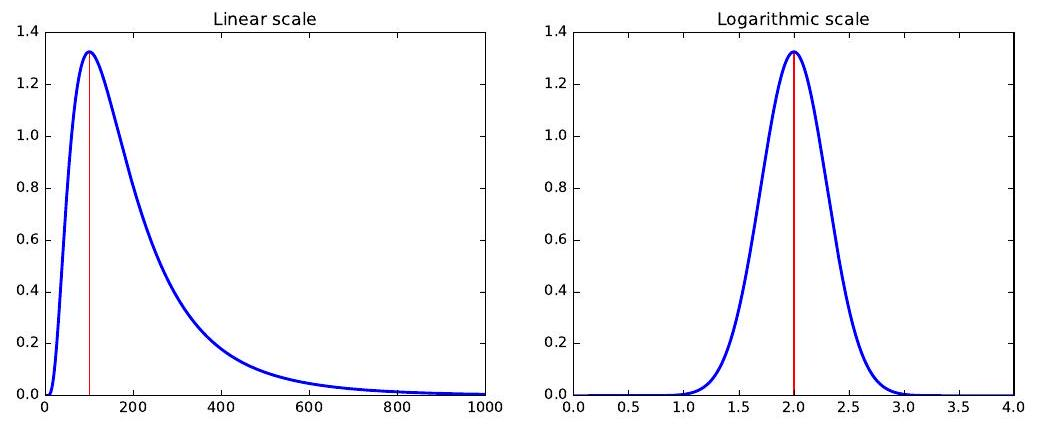
\includegraphics[max width=\textwidth]{2025_03_17_ca60ec0bfd96dcf8e028g-067}
    \caption{Hitting \textenglish{a} \textenglish{skewed} \textenglish{data} \textenglish{distribution} (\textenglish{left}) \textenglish{with} \textenglish{a} $\log$ \textenglish{often} \textenglish{yields} \textenglish{a} \textenglish{more} bell-shaped \textenglish{distribution} (\textenglish{right}).}
\end{figure}

दाहिनी ओर की पूंछ बाईं ओर की तुलना में बहुत आगे जाती है। और हम पावर लॉज पर चर्चा करते समय, अनुभाग 5.1.5 में, और भी अधिक असमान वितरण देखने के लिए बाध्य हैं। धन ऐसे वितरण का प्रतिनिधित्व करता है, जहाँ सबसे गरीब व्यक्ति के पास शून्य या शायद नकारात्मक धन होता है, औसत व्यक्ति (आशावादी रूप से) हजारों डॉलर में होता है, और बिल गेट्स इस लेखन के अनुसार\$100 बिलियन की ओर जा रहे हैं।

हमें ऐसी वितरणों को कुछ आसान में परिवर्तित करने के लिए एक सामान्यीकरण की आवश्यकता होती है। एक पावर लॉ वितरण का महत्व कम करने के लिए हमें कुछ गैर-रैखिक की आवश्यकता होती है, जो बड़े मूल्यों को अधिक विनम्र मूल्यों की तुलना में असमान रूप से कम कर देता है।

लॉगरिद्म शक्ति नियम चर के लिए पसंदीदा रूपांतरण है। अपनी लंबी-पूंछ वितरिती को लॉग से मारिए और अक्सर अच्छी चीजें होती हैं। चित्र 2.13 में दर्शायी गई वितरण \textit{लॉग सामान्य}वितरण थी, इसलिए लॉगरिद्म लेने से दाईं ओर एक परिपूर्ण घंटी-वक्र प्राप्त हुआ। शक्ति नियम वितरण वाले चर का लॉगरिद्म लेने से वे पारंपरिक वितरण के साथ अधिक संगत हो जाते हैं। उदाहरण के लिए, एक उच्च-मध्यम वर्ग के पेशेवर के रूप में, मेरी संपत्ति मेरे भूखे छात्रों से उतनी ही संख्या में लॉग दूर है जितना कि मैं बिल गेट्स से!

कभी-कभी लोगारिदम लेना बहुत अधिक कठोर होता है, और एक कम नाटकीय गैर-रेखीय परिवर्तन जैसे वर्गमूल एक वितरण को सामान्य करने के लिए बेहतर काम करता है। एक महत्वपूर्ण परीक्षण यह है कि परिवर्तनित मानों के आवृत्ति वितरण को प्लॉट करें और देखें कि क्या यह घंटी के आकार का दिखता है: अत्यधिक-समान, बीच में एक उभार के साथ। तभी आप जानते हैं कि आपके पास सही फ़ंक्शन है।\index{normalization}\index{Z-score}

% Mismatched: \chaptername{War Story: \textenglish{Fitting} \textenglish{Designer} Genes}

शब्द\textit{बायोइन्फॉर्मेटिशियन}\index{bioinformatician}जीव विज्ञान में "डेटा साइंटिस्ट" के लिए प्रयुक्त होता है, जो एक उभरता हुआ क्षेत्र है जो बड़े पैमाने पर डीएनए अनुक्रम डेटा संग्रहों का अध्ययन करता है और पैटर्न ढूंढ़ता है। अनुक्रम डेटा के साथ काम करना बहुत रुचिकर होता है, और मैं मानव जीनोम परियोजना की शुरुआत से शोध परियोजनाओं में बायोइन्फॉर्मेटिशियन की भूमिका निभाता रहा हूँ।

डीएनए क्रम चार-अक्षर वाले वर्णमाला\textit{\{A, C, G, T\}} पर आधारित स्ट्रिंग होते हैं। प्रोटीन वह सामग्री बनाते हैं जिससे हम शारीरिक रूप से बने होते हैं, और यह 20 विभिन्न प्रकार के आणविक इकाइयों की स्ट्रिंग से निर्मित होता है, जिन्हें एमिनो एसिड कहा जाता है।\textit{जीन} वे डीएनए क्रम हैं जो यह बताते हैं कि विशेष प्रोटीन कैसे बनाना है, जिसमें प्रत्येक इकाई\textit{\{A, C, G, T\}} के त्रिक\textit{कोडान} द्वारा वर्णित है।

हमारे उद्देश्यों के लिए, यह जानना पर्याप्त है कि जीनों का वर्णन करने वाले डीएनए अनुक्रमों की एक बड़ी संख्या है जो किसी विशेष वांछित प्रोटीन अनुक्रम के लिए \textit{कोड} कर सकते हैं। लेकिन इनमें से केवल एक का \textit{उपयोग} किया जाता है। मेरे जीवविज्ञानी सहयोगी और मैं यह जानना चाहते थे कि क्यों।

मूल रूप से, यह मान लिया गया था कि ये सभी भिन्न समानार्थी एन्कोडिंग्स मौलिक रूप से एक समान हैं, लेकिन अनुक्रम डेटा पर की गई सांख्यिकी ने यह स्पष्ट कर दिया कि कुछ कोडन्स का उपयोग दूसरों की तुलना में अधिक बार किया जाता है। जैविक निष्कर्ष यह है कि "कोडन्स महत्त्वपूर्ण होते हैं," और इसके अच्छे जैविक कारण हैं कि ऐसा होना चाहिए।

हम इस बात में रुचि लेने लगे कि "कोडान के आस-पास के जोड़े मायने रखते हैं।" शायद कुछ तीन-अक्षरों के जोड़े तेल और पानी की तरह होते हैं, और मिलना पसंद नहीं करते। अंग्रेज़ी में कुछ अक्षर जोड़े में क्रम की प्राथमिकताएँ होती हैं: आप अक्सर बिग्राम \textit{gh} देखते हैं बजाय \textit{hg} से। शायद यही डीएनए पर भी लागू होता हो? यदि हाँ, तो ऐसे तीन-अक्षरों के जोड़े होंगे जो डीएनए अनुक्रम डेटा में कम प्रस्तुत होंगे।

इसका परीक्षण करने के लिए, हमें एक स्कोर की आवश्यकता थी जो तुलना करे कि हम वास्तव में कितनी बार एक विशेष ट्रिपल देखते हैं (मान लीजिए\textit{x = CAT}) किसी अन्य विशेष ट्रिपल के बगल में (मान लीजिए\textit{y = GAG}), यह देखने के लिए कि यदि सब कुछ संयोग से होता तो हम क्या उम्मीद करते। मान लें कि$F(\textenglish{xy})$$xy$की आवृत्ति है, कोडोन$x$के बाद कोडोन$y$डीएनए अनुक्रम डेटाबेस में वास्तव में कितनी बार दिखाई देता है। ये कोडोन विशिष्ट अमीनो एसिड कोड करते हैं, मान लीजिए$a$और$b$क्रमशः। अमीनो एसिड$a$के लिए, इस बात की संभावना कि यह$x$द्वारा कोडित होगा$P(\textenglish{x})=F(\textenglish{x}) / F(\textenglish{a})$है, और इसी तरह$P(\textenglish{y})=F(\textenglish{y}) / F(\textenglish{b})$। तब$xy$को देखने की अपेक्षित संख्या\index{Social Network–movie}

\[ 
\text{Expected}(\textenglish{xy}) = \left(\frac{F(\textenglish{x})}{F(\textenglish{a})}\right)\left(\frac{F(\textenglish{y})}{F(\textenglish{b})}\right) F(\textenglish{ab}) 
\]

इस आधार पर, हम किसी दिए गए हेक्सामर$xy$के लिए एक कोडन पेयर स्कोर की गणना इस प्रकार कर सकते हैं:

\[ 
CPS(\textenglish{xy}) = \ln \left( \frac{\text{Observed}(\textenglish{xy})}{\text{Expected}(\textenglish{xy})}\right) = \ln \left( \frac{F(\textenglish{xy})}{\frac{F(\textenglish{x}) F(\textenglish{y})}{F(\textenglish{a}) F(\textenglish{b})} F(\textenglish{ab})} \right) 
\]

इस अनुपात के लॉगरिथम को लेने से बहुत ही अच्छे गुण उत्पन्न हुए। सबसे महत्वपूर्ण बात यह है कि स्कोर का चिन्ह अधिक प्रतिनिधित्व वाले युग्मों को कम प्रतिनिधित्व वाले युग्मों से अलग करता है। चूंकि परिमाण सममित\(+1\)की तरह ही प्रभावशाली\(-1\)था, हम इन स्कोरों को जोड़ या औसत कर सकते थे किसी जीन के लिए एक उचित स्कोर देने के लिए। हमने इन स्कोरों का उपयोग उन जीनों को डिजाइन करने के लिए किया जो वायरस के लिए खराब होने चाहिए, जिसने वैक्सीन बनाने के लिए एक रोमांचक नई तकनीक दी।

\begin{center}
\begin{tabular}{|l|l|l|l|l|}
\hline
Fr. Dep. & \textenglish{Score} &  & Fr. Ind. & \textenglish{Score} \\
\hline
\textenglish{CATAGG} & -1.74 &  & \textenglish{GGGGGG} & -1.01 \\
\hline
\textenglish{TCTAGC} & -1.61 &  & \textenglish{CCCCCC} & -0.95 \\
\hline
\textenglish{GTTAGG} & -1.58 &  & \textenglish{GGCGCC} & -0.66 \\
\hline
\textenglish{GCTAGT} & -1.48 &  & \textenglish{GGGGGT} & -0.63 \\
\hline
\textenglish{CCTAGT} & -1.44 &  & \textenglish{CGGGGG} & -0.59 \\
\hline
\textenglish{GGTAGG} & -1.41 &  & \textenglish{AGGGGG} & -0.58 \\
\hline
\textenglish{CTTAGG} & -1.40 &  & \textenglish{CACGTG} & -0.58 \\
\hline
\textenglish{ACTAGC} & -1.38 &  & \textenglish{ACCCCC} & -0.56 \\
\hline
\textenglish{GCTAGC} & -1.37 &  & \textenglish{GGGCCC} & -0.56 \\
\hline
\textenglish{GCTAGA} & -1.36 &  & \textenglish{CCCCCT} & -0.53 \\
\hline
\textenglish{CCTAGC} & -1.35 &  & \textenglish{CGCCCC} & -0.52 \\
\hline
\textenglish{GATAGG} & -1.35 &  & \textenglish{CCCCCG} & -0.51 \\
\hline
\end{tabular}
\end{center}

\begin{figure}[h]
    \centering
    \caption{Patterns \textenglish{in} \textenglish{DNA} \textenglish{sequences} \textenglish{with} \textenglish{the} \textenglish{lowest} \textenglish{codon} \textenglish{pair} \textenglish{scores} \textenglish{become} \textenglish{obvious} \textenglish{on} inspection. \textenglish{When} \textenglish{interpreted} in-frame, \textenglish{the} \textenglish{stop} \textenglish{symbol} \textenglish{TAG} \textenglish{is} \textenglish{substantially} \textenglish{depleted} (\textenglish{left}). \textenglish{When} \textenglish{interpreted} \textenglish{in} \textenglish{the} \textenglish{other} \textenglish{two} frames, \textenglish{the} \textenglish{most} \textenglish{avoided} \textenglish{patterns} \textenglish{are} \textenglish{all} \textenglish{very} \textenglish{low} complexity, \textenglish{like} \textenglish{runs} \textenglish{of} \textenglish{a} \textenglish{single} \textenglish{base} (\textenglish{right}).}
\end{figure}

यह जानना कि कुछ जोड़ी कोडॉन खराब थे, यह नहीं समझाता था कि \textit{क्यों}वे खराब थे। लेकिन दो संबंधित स्कोर्स की गणना करने (विवरण अप्रासंगिक हैं) और इसके आधार पर ट्रिपलेट्स को सॉर्ट करने से, जैसे चित्र 2.14 में दिखाया गया है, कुछ पैटर्न उभर कर सामने आए। क्या आपको पैटर्न दिखाई देते हैं? बाईं ओर की सभी खराब शृंखलाओं में \textit{TAG}शामिल है, जो एक विशेष कोडॉन है जो जीन को बंद करने का संकेत देता है। और दाईं ओर की सभी खराब शृंखलाएं \textit{C}और \textit{G}के बहुत ही सरल पुनरावृत्तिमय क्रमों में शामिल हैं। ये जैविक रूप से यह बताते हैं कि क्यों विकास द्वारा पैटर्न से बचा जाता है, जिसका अर्थ है कि हमने जीवन के बारे में कुछ बहुत अर्थपूर्ण खोज की है।

इस कहानी से दो मुख्य सबक प्राप्त होते हैं। पहला, विशिष्ट वस्तुओं के पहलुओं को उजागर करने के लिए संख्यात्मक स्कोरिंग फंक्शन विकसित करना बहुत उपयोगी हो सकता है जिससे पैटर्न दिख सके। वास्तव में, चैप्टर 4 में ऐसे सिस्टम के विकास पर ध्यान केंद्रित किया जाएगा। दूसरा, ऐसे मात्रा में लघुगणक जोड़ने से उन्हें और भी उपयोगी बनाया जा सकता है, जिससे हम पेड़ों के बीच जंगल को देख सकते हैं।

% Mismatched: \chaptername{Chapter Notes}

कई उत्कृष्ट परिमाण सिद्धांत की परिचयों उपलब्ध हैं, जिनमें \cite{tijms2012understanding, bertsekas2008introduction} शामिल है। प्रारंभिक सांख्यिकी के लिए भी यही बात लागू होती है, जिसमें अच्छे प्रारंभिक ग्रंथ \cite{james2013introduction, wheelan2013naked} शामिल हैं। इस अध्याय में परिमाण सिद्धांत का संक्षिप्त इतिहास वीवर \cite{weaver1982lady} पर आधारित है।

अपने सबसे मजबूत रूप में, प्रभावी बाजार परिकल्पना कहती है कि सार्वजनिक जानकारी का उपयोग करके शेयर बाजार को मूलतः अप्रत्याशित माना जाता है। मेरी व्यक्तिगत सलाह यह है कि आपको इंडेक्स फंडों में निवेश करना चाहिए जो सक्रिय रूप से बाजार की दिशा को भविष्यवाणी करने की कोशिश नहीं करते। माल्कियल की \textit{A \textenglish{Random} \textenglish{Walk} \textenglish{Down} \textenglish{Wall} Street}\cite{malkiel1999random}\index{Borda’s method}\index{rankings!merging}

%---- \textenglish{Page} \textenglish{End} \textenglish{Break} \textenglish{Here} ---- \textenglish{Page} : 52

% \textenglish{Page} : 52
\noindent
\textenglish{is} \textenglish{an} \textenglish{excellent} \textenglish{introduction} \textenglish{to} \textenglish{such} \textenglish{investment} thinking.\\
\textenglish{The} \textenglish{Fast} \textenglish{Fourier} \textenglish{Transform} (\textenglish{FFT}) \textenglish{provides} \textenglish{an} $O(\textenglish{n} \log \textenglish{n})$ \textenglish{time} \textenglish{algorithm} \textenglish{to} \textenglish{compute} \textenglish{the} \textenglish{full} \textenglish{autocorrelation} \textenglish{function} \textenglish{of} \textenglish{an} $n$-element sequence, \textenglish{where} \textenglish{the} \textenglish{straightforward} \textenglish{computation} \textenglish{of} $n$ \textenglish{correlations} \textenglish{takes} $O\left(n^{2}\right)$. \textenglish{Bracewell} \cite{bracewell1999fourier} \textenglish{and} \textenglish{Brigham} \cite{brigham1988fast} \textenglish{are} \textenglish{excellent} \textenglish{introductions} \textenglish{to} \textenglish{Fourier} \textenglish{transforms} \textenglish{and} \textenglish{the} FFT. \textenglish{See} \textenglish{also} \textenglish{the} \textenglish{exposition} \textenglish{in} \textenglish{Press} et.al. \cite{press2007numerical}.

चित्र 2.10 में कॉमिक स्ट्रिप रैंडल मुनरो के वेबकॉमिक\textit{xkcd} से आयी है, विशेष रूप से \href{https://xkcd.com/552}{https://xkcd.com/552}, और इसे अनुमति के साथ पुनर्मुद्रित किया गया है।

सेक्शन 2.5 की युद्ध कहानी हमारे काम के इर्द-गिर्द घूमती है, जो बताता है कि कोडॉन पेयर बायस का प्रभाव जीन के अनुवाद पर कैसे पड़ता है। चित्र 2.14 मेरे सहयोगी जस्टिन गार्डिन का योगदान है। देखें [सीपीएस$^{+}$08, एमसीपी$^{+}$10, \cite{skiena2012redesigning}] कि हमने कैसे कोडॉन पेयर बायस का उपयोग पोलियो और फ्लू जैसी वायरल बीमारियों के लिए टीकों के डिजाइन में किया।

\section{अभ्यास}
% असंगत: \subsectionname{Probability}

\begin{enumerate}
    \item[2-1.] \textbf{[3]} मान लीजिए कि $80\%$ लोग पीनट बटर पसंद करते हैं, $89\%$ जैली पसंद करते हैं, और $78\%$ दोनों पसंद करते हैं। यह दिया गया है कि एक रैंडमली चुने गए व्यक्ति को पीनट बटर पसंद है, तो यह संभावना क्या है कि उसे जैली भी पसंद है?
    \item[2-2.] \textbf{[3]} मान लीजिए कि $P(\textenglish{A})=0.3$ और $P(\textenglish{B})=0.7$।
    \begin{enumerate}
        \item क्या आप $P(\textenglish{A} \text{ और } \textenglish{B})$ निकाल सकते हैं यदि आपको केवल $P(\textenglish{A})$ और $P(\textenglish{B})$ ही पता हो?
        \item यह मानते हुए कि घटनाएँ $A$ और $B$ स्वतंत्र रैंडम प्रक्रियाओं से उत्पन्न होती हैं:
        \begin{itemize}
            \item $P(\textenglish{A} \text{ और } \textenglish{B})$ क्या है?
            \item $P(\textenglish{A} \text{ या } \textenglish{B})$ क्या है?
            \item $P(\textenglish{A} \mid \textenglish{B})$ क्या है?
        \end{itemize}
    \end{enumerate}

\item[2-3.]\textbf{[3]}एक खेल पर विचार करें जहाँ आपका स्कोर दो पासों का अधिकतम मान है। प्रत्येक घटना का संभावना$ \{1,\ldots, 6\}$ से गड़ना करें।
\item[2-4.]\textbf{[8]}सिद्ध करें कि यादृच्छिक चर$X$ से खींचे गए मानों की जोड़ी के अधिकतम का संचयी वितरण फ़ंक्शन मूल संचयी वितरण फ़ंक्शन$X$ का वर्ग है।
\item[2-5.]\textbf{[5]}यदि दो बाइनरी यादृच्छिक चर$X$ और $Y$ स्वतंत्र हैं, तो क्या$\bar{X}$(जो$X$ का पूरक है) और $Y$ भी स्वतंत्र हैं? सबूत या एक प्रति उदाहरण दें।

\index{directed \textenglish{acyclic} graph}\index{topological sorting}
\subsection{सांख्यिकी}

\begin{enumerate}
    \item[2-6.] \textbf{[3]} प्रत्येक वितरण के जोड़े की तुलना करें यह निर्णय लेने के लिए कि किसके पास अधिक माध्य और अधिक मानक विचलन है। आपको $\mu$ और $\sigma$ के वास्तविक मानों की गणना करने की आवश्यकता नहीं है, केवल यह कि वे एक दूसरे की तुलना में कैसे हैं।
    \begin{enumerate}
        \item i. $3,5,5,5,8,11,11,11,13$.
        \item ii. $3,5,5,5,8,11,11,11,20$.
        \item i. $-20,0,0,0,15,25,30,30$.
        \item ii. $-40,0,0,0,15,25,30,30$.
        \item i. $0,2,4,6,8,10$.
        \item ii. $20,22,24,26,28,30$.
        \item i. $100,200,300,400,500$.
        \item ii. $0,50,300,550,600$.
    \end{enumerate}

\item[2-7.]\textbf{[3]}एक ऎसी संभावना वितरण बनाएं जहाँ कोई भी द्रव्यमान माध्य के भीतर न हो।
$[2-8.]\textbf{[3]}मौलिक और ज्यामितीय माध्य की तुलना यादृच्छिक पूर्णांकों पर कैसे होती है?
\sigma[2-9.]\textbf{[3]}दिखाएं कि मौलिक माध्य बराबर है ज्यामितीय माध्य के जब सभी पद समान हों।
\end{enumerate}

% Mismatched: \subsectionname{Correlation Analysis}

\begin{enumerate}
    \item[2-10.] \textbf{[3]} सत्य या असत्य: -0.9 का सहसंबंध गुणांक 0.5 के तुलना में अधिक मजबूत रैखिक संबंध का संकेत देता है। समझाइए क्यों।
    \item[2-11.] \textbf{[3]} एक विशेष कंपनी में कॉलेज और हाई स्कूल स्नातकों की वार्षिक वेतन के बीच सहसंबंध गुणांक क्या होगा, यदि प्रत्येक संभव नौकरी शीर्षक के लिए कॉलेज स्नातक हमेशा हाई स्कूल स्नातकों से:
    \begin{enumerate}
        \item $\$5,000$ अधिक कमाते हैं?
        \item $25\%$ अधिक कमाते हैं?
        \item $15\%$ कम कमाते हैं?
    \end{enumerate}

\item[2-12.]\textbf{[3]}अगर पुरुष हमेशा उन महिलाओं से शादी करते जो:

\begin{enumerate}क्या \item वे स्वयं से तीन वर्ष छोटे हैं? क्या \item वे स्वयं से दो वर्ष बड़े हैं? \index{Clyde}\index{National \textenglish{Football} League}\index{point spread}क्या \item वे स्वयं से आधे हैं? \end{enumerate}

\item[2-13.]\textbf{[5]}गूगल सर्च में पाए गए डेटा या साहित्य का उपयोग करके इन के बीच सहसंबंध की ताकत का अनुमान/मापन करें:\index{football!game prediction}

\begin{enumerate}
        \item बेसबॉल में हिटर के लिए बनाए गए हिट्स और वॉक्स।
        \item बेसबॉल में पिचर्स द्वारा दी गई हिट्स और वॉक्स।
    \end{enumerate}

\item[2-14.]\textbf{[5]}समान रूप से चुने गए बिंदुओं के नमूनों के लिए पियरसन और स्पीयरमैन रैंक सहसंबंध की गणना करें$(x, x^{k})$. जब$k$बढ़ता है तो इन मानों में किस प्रकार का परिवर्तन होता है?
\end{enumerate}

% Mismatched: \subsectionname{Logarithms}

\begin{enumerate}
    \item[2-15.] \textbf{[3]} सिद्ध करें कि किसी भी संख्या का लोगारिदम जो 1 से कम हो, नकारात्मक होता है।
    \item[2-16.] \textbf{[3]} सिद्ध करें कि शून्य का लोगारिदम अपरिभाषित होता है।
    \item[2-17.] \textbf{[5]} सिद्ध करें कि
    \[
    \textenglish{x} \cdot \textenglish{y} = b^{(\log_{b} \textenglish{x} + \log_{b} \textenglish{y})}
    \]
    \item[2-18.] \textbf{[5]} एक आधार-$b$ लोगारिदम को आधार-$a$ में बदलने के सूत्र की शुद्धता को सिद्ध करें, कि
    \[
    \log_{a}(\textenglish{x}) = \frac{\log_{b}(\textenglish{x})}{\log_{b}(\textenglish{a})}
    \]
\end{enumerate}

\subsection{निर्वहन परियोजनाएँ}

\begin{enumerate}
    \item[2-19.] \textbf{[3]} कुछ रोचक डेटा सेट खोजिए, और उनके औसत और माध्यिका कितने समान हैं, इसकी तुलना कीजिए। कौन सा वितरण है जहाँ औसत और माध्यिका में सबसे अधिक अंतर होता है?
    \item[2-20.] \textbf{[3]} कुछ रोचक डेटा सेट खोजिए और सभी जोड़ों में रोचक संबंध खोजिए। शायद \href{http://www.data-manual.com/}{http://www.data-manual.com/} में उपलब्ध से प्रारंभ करें। आपको क्या मिलता है?
\end{enumerate}

\subsection{साक्षात्कार प्रश्न}

\begin{enumerate}
    \item[2-21.] \textbf{[3]} एक सिक्के के $n$ बार उछालने पर $k$ बार सिर आने की संभावना क्या है, जहाँ प्रत्येक उछाल में सिर आने की संभावना $p$ है? $k$ या अधिक बार सिर आने की संभावना क्या है?
    \item[2-22.] \textbf{[5]} मान लीजिए कि एक हर बार बदलते हुए सिक्के के $i$वें उछाल पर सिर आने की संभावना $f(\textenglish{i})$ है। आप $n$ उछालों में ठीक $k$ बार सिर आने की संभावना को कुशलता से कैसे गणना करेंगे?
    \item[2-23.] \textbf{[5]} एक बास्केटबॉल खेल के हाफ़टाइम पर आपको दो संभावित चुनौतियाँ दी जाती हैं:
    \begin{enumerate}
        \item तीन शॉट्स लें, और उनमें से कम से कम दो बनाएं।
        \item आठ शॉट्स लें, और उनमें से कम से कम पाँच बनाएं।
    \end{enumerate}

आपके पास बेहतर मौका पाने के लिए कौनसी चुनौती चुननी चाहिए?
\item[2-24.]\textbf{[3]} दस बार सिक्का उछालने पर आठ हेड्स और दो टेल्स आए। आप कैसे विश्लेषण करेंगे कि सिक्का निष्पक्ष है या नहीं?$p$-मूल्य क्या है?
\item[2-25.]\textbf{[5]} एक$n$संख्याओं की धारा दी गई है, यह दिखाएं कि केवल स्थायी भंडारण का उपयोग करके एक को यादृच्छिक रूप से समान रूप से कैसे चुनें। अगर आपको पहले से$n$पता नहीं है तो क्या करें?
\item[2-26.]\textbf{[5]} एक$k$-स्ट्रीक$n$सिक्का फ्लिप्स की श्रृंखला में तब शुरू होती है जब$i$वा फ्लिप और अगले$k-1$फ्लिप्स का परिणाम समान होता है। उदाहरण के लिए, \textenglish{HTTTHH} अनुक्रम में दूसरे, तीसरे और पांचवें टॉस से शुरू होने वाले 2-स्ट्रीक्स शामिल हैं। निष्पक्ष सिक्के की$n$टॉस में आप किस$k$-स्ट्रीक्स की अपेक्षित संख्या देखेंगे?
$[2-27.]\textbf{[5]} एक व्यक्ति एक पोकट कैलकुलेटर में आठ अंकों की संख्या को बेतरतीब ढंग से टाइप करता है। संभावना क्या है कि संख्या समान दिखेगी भले ही कैलकुलेटर को उल्टा कर दिया जाए?
$[2-28.]\textbf{[3]} आप एक पासा खेलने वाला खेल खेलते हैं जहां आपके पास दो विकल्प होते हैं:

\begin{enumerate}
        \item पासा एक बार फेंको और परिणाम संख्या के बराबर एक पुरस्कार प्राप्त करो (उदाहरण के लिए, \$3 संख्या "3" के लिए) और फिर खेल रोक दो।
        \item आप पहले पुरस्कार को उसके परिणाम के अनुसार अस्वीकार कर सकते हैं और दूसरी बार पासा फेंक सकते हैं, और उसी तरीके से पुरस्कार प्राप्त कर सकते हैं।
    \end{enumerate}

आपको अपने इनाम को अधिकतम करने के लिए कौन सी रणनीति चुननी चाहिए? यानी, पहले रोल के कौन से परिणामों के लिए आपको दूसरी गेम खेलने का विकल्प चुनना चाहिए? अगर आप दूसरी रणनीति चुनते हैं तो इनाम की सांख्यिकीय अपेक्षा क्या है?
\item[2-29.]\textbf{[3]}A/B परीक्षण क्या है और यह कैसे काम करता है?
\item[2-30.]\textbf{[3]}सांख्यिकीय स्वतंत्रता और सहसंबंध के बीच क्या अंतर है?
\item[2-31.]\textbf{[3]}हम अक्सर कहते हैं कि सहसंबंध कारणिता को इंगित नहीं करता है। इसका क्या मतलब है?
\item[2-32.]\textbf{[5]}एक तिर्यक वितरण और एक समान वितरण के बीच क्या अंतर है?
\end{enumerate}

\subsection{कैगल चैलेंजेस}

\begin{enumerate}
    \item[2-33.] कारण-प्रभाव जोड़े: सहसंबंध बनाम कारणता। \href{https://www.kaggle.com/c/cause-effect-pairs}{https://www.kaggle.com/c/cause-effect-pairs}
    \item[2-34.] एक अनुक्रम में "यादृच्छिक संख्या" की भविष्यवाणी करें। \href{https://www.kaggle.com/c/random-number-grand-challenge}{https://www.kaggle.com/c/random-number-grand-challenge}
    \item[2-35.] एक पालतू शरण में जानवरों के भविष्य की भविष्यवाणी करें। \href{https://www.kaggle.com/c/shelter-animal-outcomes}{https://www.kaggle.com/c/shelter-animal-outcomes}
\end{enumerate}

%---- \textenglish{Page} \textenglish{End} \textenglish{Break} \textenglish{Here} ---- \textenglish{Page} : 56

\chapter{डेटा मंगिंग}

\epigraph{दो अवसरों पर मुझसे पूछा गया है, "प्रार्थना करें, श्रीमान बाबेज, अगर आप मशीन में गलत आंकड़े डालते हैं, तो क्या सही उत्तर निकलेंगे?" ... मैं इस प्रकार की विचारों की भ्रम की स्थिति को सही ढंग से समझने में असमर्थ हूं जो इस तरह के प्रश्न को उकसा सकती है।}{\index{R}-- \textit{चार्ल्स बाबेज}}

अधिकांश डेटा वैज्ञानिक अपना अधिकांश समय डेटा को साफ और फ़ॉर्मेट करने में बिताते हैं। बाकी लोग अपना अधिकांश समय इस बात की शिकायत करते हुए बिताते हैं कि जो वे करना चाहते हैं, उसे करने के लिए डेटा उपलब्ध नहीं है।

इस अध्याय में, हम डेटा के साथ गणना के कुछ बुनियादी यांत्रिकी पर काम करेंगे। आँकड़े या मशीन लर्निंग जैसी उच्च स्तर की चीज़ों पर नहीं, बल्कि डेटा को खोजने और उसे साफ करने का बुनियादी काम करेंगे; इसे \textit{डेटा मन्जिंग} के नाम से जाना जाता है।

जबकि व्यावहारिक प्रश्न जैसे “उपलब्ध सर्वश्रेष्ठ लाइब्ररी या प्रोग्रामिंग भाषा कौन सी है?” स्पष्ट रूप से महत्वपूर्ण हैं, उनके उत्तर इतनी तेजी से बदलते हैं कि इस तरह की पुस्तक उन पर चर्चा करने के लिए सही स्थान नहीं है। इसलिए, मैं इस पुस्तक को किसी विशेष सॉफ़्टवेयर उपकरणों के सेट के चारों ओर आकार देने के बजाय सामान्य सिद्धांतों के स्तर पर रहूंगा। फिर भी, हम इस अध्याय में उपलब्ध संसाधनों के परिदृश्य पर चर्चा करेंगे: वे क्यों मौजूद हैं, वे क्या करते हैं, और उनका सर्वोत्तम उपयोग कैसे करें।

किसी भी डेटा साइंस परियोजना में पहला कदम सही डेटा प्राप्त करना होता है। लेकिन यह अक्सर चिंताजनक रूप से कठिन होता है। यह अध्याय डेटा संसाधनों के लिए सबसे समृद्ध शिकार क्षेत्रों का सर्वेक्षण करेगा, और फिर आपके द्वारा प्राप्त किए गए डेटा को साफ करने की तकनीकों को पेश करेगा। आपके डेटा को इस तरह से संवारना कि आप सीधे इसका विश्लेषण कर सकें, महत्वपूर्ण परिणामों के लिए आवश्यक है। जैसा कि बाबेज़ स्वयं संक्षेप में कह सकते थे, "गलत डेटा से गलत निष्कर्ष।"

\section{डेटा साइंस के लिए भाषाएँ}

सिद्धांत रूप में, हर पर्याप्त शक्तिशाली प्रोग्रामिंग भाषा किसी भी एल्गोरिदम को व्यक्त करने में सक्षम होती है जो कि गणना के योग्य है। लेकिन व्यवहार में, कुछ प्रोग्रामिंग भाषाएँ विशिष्ट कार्यों में दूसरों की तुलना में कहीं बेहतर सिद्ध होती हैं। यहाँ बेहतर का मतलब हो सकता है\textit{प्रोग्रामर के लिए आसान}या शायद\textit{अधिक गणनात्मक रूप से दक्ष}, यह मिशन पर निर्भर करता है।

मुख्य डेटा विज्ञान प्रोग्रामिंग भाषाएँ जिन्हें जानना आवश्यक है, वे हैं:



शायद \textenglish{Python} के खिलाफ सबसे बड़ा तर्क दक्षता है: इंटरप्रेटेड भाषाएँ गति के लिए संकलित भाषाओं से प्रतिस्पर्धा नहीं कर सकतीं। लेकिन \textenglish{Python} कंपाइलर किसी हद तक मौजूद हैं, और दक्षतापूर्ण C/असेम्बली भाषा लाइब्रेरियों को जोड़ने का समर्थन करते हैं जो गणनात्मक-गहन कार्यों के लिए हैं। मूल रूप से, आपके द्वारा प्रस्तुत इस पुस्तक में सामग्री के माध्यम से काम करने के लिए \textenglish{Python} शायद आपका प्राथमिक उपकरण होना चाहिए।
  
\item\textit{पर्ल}:\index{Perl} यह\textit{उपयोग}वेब पर डेटा मंगिंग के लिए प्रमुख भाषा हुआ करती थी, इसके पहले कि \textenglish{Python} ने इसे पछाड़ दिया। \textenglish{TIOBE} प्रोग्रामिंग भाषा की लोकप्रियता सूचकांक (\href{http://www.tiobe.com/tiobe-index}{http://www.tiobe.com/tiobe-index}) में, 2008 में \textenglish{Python} ने पहली बार पर्ल से लोकप्रियता में बढ़त ली और पीछे मुड़कर नहीं देखा। इसके कई कारण हैं, जिनमें वस्तु-उन्मुख प्रोग्रामिंग के लिए मजबूत समर्थन और बेहतर उपलब्ध लाइब्रेरियाँ शामिल हैं, लेकिन असल में इस समय पर्ल में प्रोजेक्ट्स शुरू करने के लिए बहुत कम अच्छे कारण हैं। हालांकि, यदि आप इसे किसी विरासत प्रोजेक्ट में पाते हैं तो आश्चर्यचकित मत होइए।

\item\textit{आर}: यह आँकड़ों के वैज्ञानिकों की प्रोग्रामिंग भाषा है, जिसमें डेटा विश्लेषण और दृश्य-प्रस्तुति के लिए सबसे गहरी पुस्तकालयें उपलब्ध हैं। डेटा विज्ञान की दुनिया @⸨आर⸩ और पाइथन के खेमों में विभाजित है, जहाँ शायद @⸨आर⸩ अन्वेषण के लिए अधिक उपयुक्त है और पाइथन उत्पादन उपयोग के लिए बेहतर है। @⸨आर⸩ के साथ बातचीत की शैली कुछ हद तक एक स्वाभाविक लगती है, इसलिए मैं आपको प्रोत्साहित करता हूँ कि आप इसे थोड़ा खेलने की कोशिश करें ताकि यह देख सकें कि यह आपको स्वाभाविक लगता है या नहीं।

लिंकजेस आर और पाइथन के बीच मौजूद हैं, इसलिए आप आसानी से पाइथन कोड में आर लाइब्रेरी फंक्शंस को कॉल कर सकते हैं। इससे उन्नत सांख्यिकी विधियों की पहुंच मिलती है, जो हो सकता है कि नेटिव पाइथन लाइब्रेरीज़ द्वारा समर्थित नहीं हों।

\item\textit{मैटलैब}:\index{Matlab} यहाँ मैट का अर्थ है \textit{मैट्रिक्स}, क्योंकि मैटलैब एक भाषा है जो मैट्रिसेज के तीव्र और कुशल संचालन के लिए बनाई गई है। जैसे हम देखेंगे, कई मशीन लर्निंग एल्गोरिदम मैट्रिसेज पर संचालन में कमी कर देते हैं, जिससे मैटलैब उच्च स्तर पर अमूर्तीकरण में प्रोग्राम करने वाले अभियंताओं के लिए एक स्वाभाविक विकल्प बन जाता है।

मैटलैब एक मालिकाना प्रणाली है। हालांकि, इसके अधिकतर कार्यक्षमता जीएनयू ऑक्टेव, एक ओपन-सोर्स विकल्प में उपलब्ध हैं।
  
\item\textit{जावा और सी/सी++}: बड़े सिस्टम के विकास के लिए ये मुख्यधारा के प्रोग्रामिंग भाषा हैं और ये बड़े डेटा अनुप्रयोगों में महत्वपूर्ण हैं। हडूप और स्पार्क जैसे पैरेलल प्रोसेसिंग सिस्टम क्रमशः जावा और सी++ पर आधारित हैं। यदि आप वितरित कंप्यूटिंग की दुनिया में रह रहे हैं, तो आप यहाँ सूचीबद्ध अन्य भाषाओं की जगह जावा और सी++ की दुनिया में रह रहे हैं।
  
\item\textit{मथमैटिका/वोल्फ्राम अल्फा}: मथमैटिका एक मालिकाना प्रणाली है जो अंकीय और प्रतीकात्मक गणित के सभी पहलुओं के लिए संगणन समर्थन प्रदान करती है, कम मालिकाना वोल्फ्राम प्रोग्रामिंग भाषा के आधार पर बनी होती है। यह वोल्फ्राम अल्फा गणनात्मक ज्ञान इंजन की नींव है, जो एल्गोरिदम और पूर्व-पचाए हुए डेटा स्रोतों के मिश्रण के माध्यम से प्राकृतिक भाषा-जैसे प्रश्नों को संसाधित करता है। इसे \href{http://www.wolframalpha.com}{wolframalpha.com}.\index{exercises}\index{learning \textenglish{to} rank} पर देखें।

मुझे मैथमेटिका के लिए एक विशेष लगाव है। जब मैं कोई छोटा डेटा विश्लेषण या सिमुलेशन कर रहा होता हूँ, तो आमतौर पर मैं इसे ही उठाता हूँ, लेकिन लागत ने इसे पारंपरिक रूप से कई उपयोगकर्ताओं की पहुँच से बाहर कर दिया है। वोल्फ्राम भाषा की रिलीज़ शायद अब इसे एक व्यापक समुदाय के लिए खोल देती है।
  
\item\textit{एक्सेल}: स्प्रेडशीट प्रोग्राम जैसे एक्सेल अन्वेषणात्मक डेटा विश्लेषण के लिए शक्तिशाली उपकरण हैं, जैसे कि दिए गए डेटा सेट के साथ खेलना और देखना कि इसमें क्या है। ऐसे अनुप्रयोगों के लिए वे हमारे सम्मान के पात्र हैं।

पूर्ण विशेषताओं वाले स्प्रेडशीट कार्यक्रमों में पावर उपयोगकर्ताओं के लिए चौंकाने वाली मात्रा में छुपी हुई कार्यक्षमता होती है। मेरे एक छात्र, जो माइक्रोसॉफ़्ट के एक कार्यकारी बने, ने मुझे बताया कि एक्सेल के लिए 25\% सभी नई फीचर अनुरोधों की प्रस्तावित कार्यक्षमता वहाँ पहले से ही मौजूद होती है। विशेष कार्य और डेटा प्रबंधन सुविधाएँ जो आप चाहते हैं शायद एक्सेल में मौजूद होती हैं अगर आप गौर से खोजें, उसी प्रकार से जैसे आपको शायद पायथन लाइब्रेरी मिल जाएगी यदि आप उसे ढूंढे।
\end{itemize}

\subsection{नोटबुक वातावरणों का महत्व}

डेटा साइंस प्रोजेक्ट के लिए मुख्य परिणाम कोई प्रोग्राम नहीं होना चाहिए। यह कोई डेटा सेट नहीं होना चाहिए। यह आपके डेटा पर प्रोग्राम चलाने के परिणाम नहीं होना चाहिए। यह सिर्फ एक लिखित रिपोर्ट नहीं होना चाहिए।

हर डेटा साइंस परियोजना का अंतिम परिणाम एक गणनीय नोटबुक होनी चाहिए जो कोड, डेटा, गणनात्मक परिणाम, और आपके द्वारा प्रक्रिया में सीखा गया लिखित विश्लेषण को जोड़ती है। चित्र 3.1 एक जुपिटर/आईपाइथन नोटबुक से एक अंश प्रस्तुत करता है, जो दिखाता है कि कैसे यह कोड, ग्राफिक्स, और प्रलेखन को एक वर्णनात्मक दस्तावेज़ में एकीकृत करता है जिसे एक प्रोग्राम की तरह निष्पादित किया जा सकता है।

कारण यह है कि संगणनात्मक परिणाम लंबे मापदंड चयन और डिज़ाइन निर्णयों की श्रृंखलाओं का उत्पाद होते हैं। यह कई समस्याएँ उत्पन्न करता है जिन्हें नोटबुक कम्प्यूटिंग पर्यावरण द्वारा हल किया जाता है:

\footnotetext{पूर्ण खुलासा: मैं स्टेफेन वोल्फ्राम को तीस वर्षों से अधिक समय से जानता हूँ। वास्तव में, हमने साथ मिलकर आईपैड का आविष्कार किया था \cite{barron2010apple}.}

%---- \textenglish{Page} \textenglish{End} \textenglish{Break} \textenglish{Here} ---- \textenglish{Page} : 59







\begin{verbatim}
\textenglish{degrees} = range(1, 8)
\textenglish{errors} = np.array([regressor3(\textenglish{d}) \textenglish{for} \textenglish{d} \textenglish{in} degrees])
plt.plot(degrees, errors[:, 0], marker='^', c='r', label='Testing samples')
plt.plot(degrees, errors[:, 1], marker='o', c='b', label='Training sample')
plt.yscale('log')
plt.xlabel("degree"); plt.ylabel("Error")
plt.legend(loc='best')
\end{verbatim}



डिग्री को बदलते हुए, हम मॉडल प्रदर्शन के दो क्षेत्र खोजते हैं:

\begin{itemize}
  \item अंडरफिटिंग (डिग्री $\leq 3$): इस तथ्य की विशेषता है कि परीक्षण त्रुटि कम हो जाती है यदि हम मॉडल क्षमता को बढ़ाते हैं।
  \item ओवरफिटिंग (डिग्री $> 3$): इस तथ्य की विशेषता है कि परीक्षण बढ़ जाता है यदि हम मॉडल क्षमता को बढ़ाते हैं। ध्यान दें, कि प्रशिक्षण त्रुटि कम हो रही है या यथावत रह रही है।
\end{itemize}

\subsection{मानक डेटा प्रारूप}
\index{data formats}
डेटा विभिन्न स्रोतों से आता है, और विभिन्न प्रकार के प्रारूपों में होता है। कौन-सा प्रस्तुतीकरण सबसे अच्छा है, यह इस पर निर्भर करता है कि अंतिम उपभोक्ता कौन है। चार्ट्स और ग्राफ्स संख्यात्मक डेटा का मतलब लोगों तक पहुँचाने के अद्भुत तरीके हैं। वास्तव में, अध्याय 6 डेटा के दृश्यांकन की तकनीकों पर केंद्रित होगा। लेकिन ये चित्र डेटा के साथ गणना करने के स्रोत के रूप में मूल रूप से बेकार होते हैं। मुद्रित मानचित्रों से गूगल मानचित्र तक एक लंबा सफर होता है।

श्रेष्ठ संगणकीय डेटा प्रारूपों के पास कई उपयोगी गुण होते हैं:

\begin{itemize}
  \item \textit{वे कंप्यूटरों के लिए पार्स करने में आसान हैं:} उपयोगी प्रारूप में लिखे गए डेटा का उद्देश्य उसे अन्यत्र फिर से उपयोग करना होता है। परिष्कृत डेटा प्रारूप अक्सर एपीआई द्वारा समर्थित होते हैं जो तकनीकी विवरणों का प्रबंधन करते हैं और सही प्रारूप सुनिश्चित करते हैं।
  \item \textit{वे लोगों के लिए पढ़ने में आसान हैं:} डेटा को देखना कई संदर्भों में एक आवश्यक कार्यवाही है। इस निर्देशिका में मौजूद कौन सा डेटा फ़ाइल मेरे उपयोग के लिए सही है? हम इस फ़ाइल के डेटा फील्ड्स के बारे में क्या जानते हैं? प्रत्येक विशेष फील्ड के लिए मूल्यों की सकल श्रेणी क्या है?\index{bell-shaped}\index{binomial distribution}\index{independence}\index{Pascal’s triangle}
\end{itemize}

इन उपयोग मामलों में डेटा फ़ाइल को टेक्स्ट एडिटर में खोलकर देखने की क्षमता के अद्भुत मूल्य को दर्शाया गया है। आमतौर पर, इसका मतलब है कि डेटा को एक मानवीय-पठनीय टेक्स्ट-कोडेड प्रारूप में प्रस्तुत करना, जिसमें रिकार्ड्स को अलग-अलग लाइनों द्वारा चिह्नित किया जाता है, और फ़ील्ड्स को सीमांकित प्रतीकों द्वारा अलग किया जाता है।\index{statistical distributions}

%---- \textenglish{Page} \textenglish{End} \textenglish{Break} \textenglish{Here} ---- \textenglish{Page} : 61

\itemवे अन्य उपकरणों और सिस्टमों द्वारा व्यापक रूप से उपयोग किए जाते हैं: कॉर्पोरेट हृदय में स्वामित्व डेटा मानक आविष्कार करने की इच्छा दृढ़ता से धड़कती है, और अधिकांश सॉफ्टवेयर डेवलपर एक टूथब्रश साझा करने की अपेक्षा एक फ़ाइल फ़ॉर्मैट साझा करना पसंद नहीं करेंगे। लेकिन ये ऐसे आवेग हैं जिनसे बचना चाहिए। डेटा की शक्ति अन्य डेटा संसाधनों के साथ मिलाने और मिलान करने से आती है, जिसे लोकप्रिय मानक फ़ॉर्मैट का उपयोग करके सबसे अच्छा सुगम बनाया जाता है।
\end{itemize}

एक गुण जिसे मैंने इस सूची से छोड़ दिया है वह है \textit{ससंक्षिप्तता}, क्योंकि यह सामान्यत: आधुनिक कंप्यूटिंग प्रणालियों पर चलने वाले अधिकांश अनुप्रयोगों के लिए प्राथमिक चिंता का विषय नहीं होता है। डेटा भंडारण लागतों को न्यूनतम करने की खोज अक्सर अन्य लक्ष्यों के खिलाफ काम करती है। चतुराई से कई क्षेत्रों को पूर्णांक के उच्च-क्रम बिट्स में पैक करने से स्थान की बचत होती है, लेकिन इसकी कीमत इसे असंगत और अपठनीय बनाने की होती है।

सामान्य संपीड़न उपयोगिताएँ जैसे \textenglish{gzip} मानव-मित्रपूर्ण स्वरूपण की पुनरावृत्ति को अविश्वसनीय रूप से अच्छे तरीके से हटाती हैं। डिस्क की कीमतें अविश्वसनीय रूप से सस्ती हैं: जब मैं यह लिख रहा हूँ, आप लगभग \$100 में 4TB ड्राइव खरीद सकते हैं, जो एक कड़ा स्वरूपण प्रोग्रामिंग में बर्बाद किए जाने वाले एक घंटे के डेवलपर समय की लागत से कम है। जब तक आप \textenglish{Facebook} या \textenglish{Google} के पैमाने पर कार्य नहीं कर रहे हैं, संक्षिप्तता का उतना महत्व नहीं होता जितना आप सोचते हैं।\footnote{वास्तव में, मेरे \textenglish{Google} के मित्र मुझे आश्वस्त करते हैं कि वे अक्सर पेटाबाइट पैमाने पर भी स्थान के मामले में सुस्त रहते हैं।}

सबसे महत्वपूर्ण डेटा प्रारूप/प्रदर्शनों के बारे में नीचे चर्चा की गई है:

\begin{itemize}
  \item \textit{CSV (कॉमा सेपरेटेड वैल्यू)} फाइलें: ये फाइलें प्रोग्राम्स के बीच डेटा का आदान-प्रदान करने के लिए सबसे सरल, सबसे लोकप्रिय फॉर्मेट प्रदान करती हैं। कि प्रत्येक पंक्ति एक ही अभिलेख का प्रतिनिधित्व करती है, जिसमें फील्ड्स को कॉमा से अलग किया जाता है, निरीक्षण से स्पष्ट है। लेकिन विशेष वर्ण और टेक्स्ट स्ट्रिंग्स के चारों ओर सूक्ष्मताएं होती हैं: क्या होगा अगर आपके नामों के बारे में डेटा में एक कॉमा हो, जैसे "थर्स्टन हॉवेल, जूनियर"? सीएसवी फॉर्मेट ऐसे चरित्रों को एस्केप कोड करने के तरीके प्रदान करता है ताकि उन्हें डिलीमीटर के रूप में नहीं माना जाए, लेकिन यह गड़बड़ है। एक बेहतर विकल्प है कि एक कम सामान्य डिलीमीटर चरित्र का उपयोग किया जाए, जैसे \textit{tsv या टैब सेपरेटेड वैल्यू} फाइलें।\\
यह परीक्षण करने का सबसे अच्छा तरीका है कि आपकी सीएसवी फाइल सही ढंग से स्वरूपित है या नहीं, यह है कि माइक्रोसॉफ्ट एक्सेल या कुछ अन्य स्प्रेडशीट प्रोग्राम इसे बिना परेशानी के पढ़ सकता है। सुनिश्चित करें कि हर प्रोजेक्ट के परिणाम इस परीक्षण को पास करते हैं जैसे ही पहली सीएसवी फाइल लिखी गई हो, ताकि बाद में परेशानी से बचा जा सके।
  \item \textit{XML (एक्स्टेंसिबल मार्कअप लैंग्वेज)}: संरचित लेकिन गैर-टैबुलर डेटा अक्सर एनोटेशन के साथ टेक्स्ट के रूप में लिखा जाता है। एक नामित-इकाई टैगर प्राकृतिक आउटपुट टेक्स्ट के प्रासंगिक उपस्ट्रिंग्स को व्यक्ति, स्थान, या वस्तु का संकेत देने वाले ब्रैकेट्स में लपेटता है। मैं इस किताब को लैटेक्स में लिख रहा हूँ, एक स्वरूपण भाषा जिसमें गणितीय अभिव्यक्तियों के चारों ओर ब्रैकेटिंग कमांड्स और \textit{italicized text} होते हैं। सभी वेबपेज \textenglish{HTML} में लिखे जाते हैं, हाइपरटेक्स्ट मार्कअप लैंग्वेज जो दस्तावेजों को \texttt{<b>} और \texttt{</b>} जैसे ब्रैकेटिंग कमांड्स का उपयोग करके \textbf{bold \textenglish{faced} text} को संलग्न करता है।\\
\textenglish{XML} ऐसी मार्कअप भाषाओं के विनिर्देश लिखने के लिए एक भाषा है। एक सही \textenglish{XML} विनिर्देश उपयोगकर्ता को विनिर्देश का पालन करने वाले किसी भी दस्तावेज़ को पार्स करने में सक्षम बनाता है। ऐसे विनिर्देशों को डिज़ाइन करना और पूरी तरह से पालन करना
\end{itemize}

उनके लिए अनुशासन की आवश्यकता होती है, लेकिन यह सार्थक होता है। हमारे लिडिया टेक्स्ट विश्लेषण प्रणाली के पहले संस्करण में, हमने अपने मार्कअप्स को "स्यूडो-एक्सएमएल" में लिखा था, जिसे एड हॉक पार्सर्स द्वारा पढ़ा जाता था जो 99% दस्तावेज़ों को सही ढंग से संभालते थे, लेकिन हर बार जब हम उन्हें विस्तारित करने की कोशिश करते तो वे टूट जाते थे। \textenglish{XML} पर एक दर्दनाक स्विच के बाद, सब कुछ अधिक विश्वसनीय\textit{और}अधिक कुशलता से काम किया, क्योंकि हम अपने विशिष्टताओं को लागू करने के कठिन कार्य को संभालने के लिए तेज़, ओपन-सोर्स \textenglish{XML} पार्सर्स को तैनात कर सकते थे।

\begin{itemize}
  \item \textit{एसक्यूएल (\textenglish{structured} \textenglish{query} \textenglish{language}) डेटाबेस}: स्प्रेडशीट्स स्वाभाविक रूप से डेटा की एकल तालिकाओं के चारों ओर संरचित होती हैं। इसके विपरीत, संवीक्ष्णीय डेटाबेस कई भिन्न लेकिन संबंधित तालिकाओं को संचालित करने में उत्कृष्ट होते हैं, एसक्यूएल का उपयोग करके एक जटिल लेकिन शक्तिशाली क्वेरी भाषा प्रदान करते हैं।\\
कोई भी उचित डेटाबेस प्रणाली \textenglish{csv} या \textenglish{XML} फ़ाइलों के रूप में रिकॉर्ड आयात और निर्यात करती है, साथ ही एक आंतरिक सामग्री डंप के रूप में। डेटाबेस में आंतरिक प्रतिनिधित्व अस्पष्ट होता है, इसलिए उन्हें डेटा फ़ॉर्मेट के रूप में विवरण देना वास्तव में सटीक नहीं होता। फिर भी, मैं उन्हें यहाँ इसलिए उजागर कर रहा हूँ क्योंकि एसक्यूएल डेटाबेस \index{SQL databases}आम तौर पर कई डेटा फ़ाइलों को मनमाने ढंग से संचालित करने की तुलना में एक बेहतर और अधिक शक्तिशाली समाधान साबित होते हैं।
  \item \textit{JSON (जावास्क्रिप्ट ऑब्जेक्ट नोटेशन)}:\index{JSON} यह कार्यक्रमों के बीच डेटा ऑब्जेक्ट्स को प्रेषित करने का एक फ़ॉर्मेट है। यह चर/डेटा संरचनाओं की स्थिति को एक प्रणाली से दूसरी प्रणाली में संचारित करने का एक स्वाभाविक तरीका है। यह प्रतिनिधित्व मूल रूप से विशेषता-मूल्य जोड़े की एक सूची होती है जो चर/फ़ील्ड नामों के अनुरूप होती है, और संबंधित मूल्य:\index{financial market}\index{normal distribution!implications}\index{stock market}\index{Poisson distribution}
\end{itemize}

\begin{verbatim}
{"employees":[
    {"firstName":"John", "lastName":"Doe"},
    {"firstName":"Anna", "lastName":"Smith"},
    {"firstName":"Peter", "lastName":"Jones"}
]}
\end{verbatim}

क्योंकि लाइब्रेरी फंक्शन्स जो \textenglish{JSON} ऑब्जेक्ट्स को पढ़ने और लिखने का समर्थन करती हैं, सभी आधुनिक प्रोग्रामिंग भाषाओं में आसानी से उपलब्ध हैं, यह डेटा संरचनाओं को बाद में उपयोग के लिए संग्रहीत करने का एक बहुत ही सुविधाजनक तरीका बन गया है। \textenglish{JSON} ऑब्जेक्ट्स इंसानों द्वारा पढ़े जा सकते हैं, लेकिन दिखने में काफी अव्यवस्थित होते हैं, जब रिकॉर्ड्स के ऐरे पेश करने की बात आती है, \textenglish{CSV} फाइल्स की तुलना में। इन्हें जटिल संरचित ऑब्जेक्ट्स के लिए प्रयोग करें, लेकिन सरल डेटा की तालिकाओं के लिए नहीं।

\begin{itemize}
  \item \textit{प्रोटोकॉल बफर्स}: ये एप्लिकेशन के बीच संचार और भंडारण के लिए संरचित डेटा को क्रमबद्ध करने का एक भाषा/प्लेटफ़ॉर्म निरपेक्ष तरीका हैं। ये \textenglish{XML} के हल्के वजन वाले संस्करण हैं (जहां आप अपने संरचित डेटा का प्रारूप परिभाषित करते हैं), जिन्हें \textenglish{JSON} की तरह प्रोग्रामों के बीच छोटे डेटा की संचार के लिए डिज़ाइन किया गया है। यह डेटा प्रारूप \textenglish{Google} में बहुत से अंतर मशीन संचार के लिए उपयोग किया जाता है। अपाचे थ्रिफ्ट एक संबंधित मानक है, जिसका उपयोग फेसबुक में होता है।
\end{itemize}

%---- \textenglish{Page} \textenglish{End} \textenglish{Break} \textenglish{Here} ---- \textenglish{Page} : 63

\begin{itemize}कुछ\end{itemize}

\section{डेटा एकत्र करना}
किसी भी डेटा विज्ञान या मॉडलिंग परियोजना में सबसे महत्वपूर्ण मुद्दा सही डेटा सेट की खोज करना है। उपयुक्त डेटा स्रोतों की पहचान करना एक कला है, जो तीन मौलिक प्रश्नों के इर्द-गिर्द घूमती है:

\begin{itemize}
  \item \textit{किसके पास वास्तव में वह डेटा हो सकता है जिसकी मुझे आवश्यकता है?}
  \item \textit{वह इसे मेरे लिए उपलब्ध कराने का निर्णय क्यों ले सकते हैं?}
  \item \textit{मैं इसे कैसे प्राप्त कर सकता हूं?}
\end{itemize}

इस खंड में, हम इन प्रश्नों के उत्तरों का अन्वेषण करेंगे। हम सामान्य डेटा के स्रोतों को देखेंगे, और आप क्या पाने की संभावना रखते हैं और क्यों। इसके बाद हम मुख्य तरीकों की समीक्षा करेंगे, जिनसे हमें पहुंच मिलती है, जिसमें एपीआई, स्क्रैपिंग और लॉगिंग शामिल हैं।

\subsection{शिकार}
डेटा किसके पास है, और आप इसे कैसे प्राप्त कर सकते हैं? कुछ संभावित संदिग्ध नीचे समीक्षा किए गए हैं।

\subsubsection{कंपनियाँ और स्वामित्व डेटा स्रोत}
बड़ी कंपनियाँ जैसे फेसबुक, गूगल, अमेजन, अमेरिकन एक्सप्रेस, और ब्लू क्रॉस के पास उपयोगकर्ताओं और लेनदेन के बारे में आश्चर्यजनक मात्रा में रोमांचक डेटा है, जो दुनिया के काम करने के तरीके को सुधारने के लिए इस्तेमाल किया जा सकता है। समस्या यह है कि बाहरी पहुँच प्राप्त करना आमतौर पर असंभव है। कंपनियाँ दो अच्छे कारणों के लिए डेटा साझा करने में हिचकिचाती हैं:

\begin{itemize}
  \item \textit{व्यापार मुद्दे}, और उनकी प्रतिस्पर्धा की मदद करने का डर।
  \item \textit{गोपनीयता मुद्दे}, और उनके ग्राहकों को अपमानित करने का डर।
\end{itemize}

एक दिल छू लेने वाली कहानी तब हुई जब \textenglish{AOL} ने विद्वानों को अपने खोज इंजन से लाखों प्रश्नों के डेटा सेट प्रदान किया, जिसे पहचान योग्य जानकारी से सावधानीपूर्वक हटा दिया गया था। विद्वानों ने सबसे पहले जो खोजा वह यह था कि सबसे अधिक बार दर्ज किए गए प्रश्न, \textenglish{Google} जैसे अन्य खोज इंजनों पर जाने के लिए हताश प्रयास थे। इससे \textenglish{AOL} खोज की गुणवत्ता में सार्वजनिक विश्वास बढ़ाने के लिए कुछ भी नहीं हुआ।

उनकी दूसरी खोज यह थी कि सर्च क्वेरीज़ को अनोनिमाइज़ करना जितना पहले सोचा गया था, उससे कहीं अधिक कठिन साबित हुआ। निश्चित रूप से आप उपयोगकर्ता नामों को आईडी नंबरों से बदल सकते हैं, लेकिन यह समझना इतना कठिन नहीं है कि लॉन्ग आइलैंड पर बार-बार \textit{स्टीवन स्कीना}, \textit{स्टोनी ब्रुक}, और \href{https://twitter.com/search?q=Skiena\&src=sprv}{https://twitter.com/search?q=Skiena\&src=sprv} की क्वेरी करने वाला व्यक्ति कौन है। वास्तव में, जैसे ही यह सार्वजनिक हुआ कि इस डेटा रिलीज़ द्वारा लोगों की पहचान उजागर हो गई थी, जिम्मेदार पक्ष को निकाल दिया गया और डेटा सेट गायब हो गया। उपयोगकर्ता की निजता महत्वपूर्ण है, और डेटा विज्ञान के चारों ओर नैतिक मुद्दों पर अनुभाग 12.7 में चर्चा की जाएगी।

इसलिए यह मत सोचिए कि आप कंपनियों से गोपनीय यूज़र डेटा जारी करने के लिए मीठी बातें करके मना लेंगे। हालाँकि, कई ज़िम्मेदार कंपनियाँ जैसे\textit{The \textenglish{New} \textenglish{York} Times}, Twitter, Facebook, और \textenglish{Google} कुछ डेटा जारी करती हैं, जो आमतौर पर ⸨दऱ-सीमित एप्लिकेशन प्रोग्राम इंटरफेसेस⸩ \index{application \textenglish{program} interfaces}(\textenglish{APIs}) द्वारा किया जाता है। उनके आमतौर पर दो उद्देश्यों होते हैं:

\begin{itemize}
  \item ग्राहकों और तीसरे पक्षों को डेटा प्रदान करना जो बिक्री बढ़ा सकता है। उदाहरण के लिए, क्वेरी फ्रीक्वेंसी और विज्ञापन मूल्य निर्धारण के बारे में डेटा जारी करना अधिक लोगों को एक दिए गए प्लेटफार्म पर विज्ञापन देने के लिए प्रोत्साहित कर सकता है।
  \item आमतौर पर कंपनी के लिए यह बेहतर होता है कि वे अच्छी तरह से व्यवहार करने वाले एपीआई प्रदान करें बजाय इसके कि कैहबॉय लगातार उनकी साइट पर हमला करें और उसे स्क्रैप करें।
\end{itemize}

इसलिए स्क्रैपिंग पर अनुभाग 3.2.2 पढ़ने से पहले एक सार्वजनिक एपीआई की तलाश करें। आपको बिल्कुल वैसा सामग्री या मात्रा नहीं मिलेगी जिसका आपने सपना देखा है, लेकिन शायद कुछ ऐसा मिलेगा जो शुरुआत करने के लिए पर्याप्त होगा। सीमाओं और उपयोग की शर्तों से अवगत रहें।

अन्य संगठन ऑफलाइन विश्लेषण के लिए रोचक डेटा के बल्क डाउनलोड प्रदान करते हैं, जैसे ⸨गूगल⸩ एनग्राम्स, ⸨आईएमडीबी⸩, और टैक्सी किराया डेटा सेट जो अध्याय 1 में चर्चा की गई है। बड़े डेटा सेट अक्सर मूल्यवान मेटाडेटा के साथ आते हैं, जैसे पुस्तक शीर्षक, छवि कैप्शन और संपादन इतिहास, जिन्हें उचित कल्पना के साथ पुनः-उपयोग किया जा सकता है।

अंततः, अधिकांश संगठनों के पास अपने व्यवसाय से संबंधित आंतरिक डेटा सेट होते हैं। एक कर्मचारी के रूप में, जब आप वहाँ काम कर रहे हों, तब आपको विशेषाधिकार प्राप्त पहुंच प्राप्त होनी चाहिए। इसके अतिरिक्त, यह जानें कि कंपनियों की आंतरिक डेटा एक्सेस नीतियाँ होती हैं, इसलिए आप कुछ प्रतिबंधों के अधीन रहेंगे। इन नीतियों के नियमों का उल्लंघन करना पूर्व-कर्मचारी बनने का एक उत्कृष्ट तरीका है।

\subsubsection{सरकार के डेटा स्रोत}
\index{government data}डेटा एकत्र करना सरकारों द्वारा किए जाने वाले महत्वपूर्ण कार्यों में से एक है। वास्तव में, संयुक्त राज्य अमेरिका द्वारा अपनी जनसंख्या की जनगणना करना हमारे संविधान द्वारा अनिवार्य किया गया है, और यह 1790 से हर दस वर्ष में समय पर चल रही है।

शहर, राज्य, और संघीय सरकारें ओपन डेटा के लिए बढ़ती हुई प्रतिबद्ध हो गई हैं, ताकि नए अनुप्रयोगों को सुगम बनाया जा सके और सरकार के मिशन को बेहतर तरीके से पूरा किया जा सके। वेबसाइट \href{http://Data.gov}{http://Data.gov} संघीय सरकार की एक पहल है, जो केंद्रीय रूप से अपने डेटा स्रोतों को इकट्ठा करने के लिए है, और अंतिम गिनती में यह 100,000 से अधिक डेटा सेट की ओर इशारा करती है!

सरकारी डेटा औद्योगिक डेटा से भिन्न होता है क्योंकि, सिद्धांत रूप से, यह जनता का होता है। \textit{सूचना का अधिकार अधिनियम}\index{Freedom \textenglish{of} \textenglish{Information} Act}\index{Freedom \textenglish{of} \textenglish{Information} Act}(एफओआई) किसी भी नागरिक को किसी भी सरकारी दस्तावेज़ या डेटा सेट के लिए औपचारिक अनुरोध करने की अनुमति देता है। इस तरह का अनुरोध यह निर्धारित करने की प्रक्रिया को प्रकट करता है कि राष्ट्रीय हित को खतरे में डाले बिना या गोपनीयता का उल्लंघन किए बिना क्या जारी किया जा सकता है।

राज्य सरकारें पचास अलग-अलग कानूनों के तहत कार्य करती हैं, इसलिए जो डेटा एक क्षेत्राधिकार में सख्ती से रखा जाता है, वह अन्य में स्वतंत्र रूप से उपलब्ध हो सकता है। न्यूयॉर्क जैसे प्रमुख शहरों में कई राज्यों की तुलना में बड़े डेटा प्रोसेसिंग ऑपरेशन होते हैं, फिर से प्रतिबंध स्थान के अनुसार भिन्न होते हैं।

%---- \textenglish{Page} \textenglish{End} \textenglish{Break} \textenglish{Here} ---- \textenglish{Page} : 65

% \textenglish{Ensuring} \textenglish{correct} \textenglish{chapter} \textenglish{formatting}

मैं सरकार के रिकॉर्ड के बारे में सोचने के लिए निम्नलिखित तरीका सुझाता हूँ। यदि ऑनलाइन खोजने के बाद आपको अपनी आवश्यक जानकारी नहीं मिलती है, तो विचार करें कि कौन सी एजेंसी संभवतः उसे रख सकती है। उनसे मित्रवत कॉल करें यह जानने के लिए कि वे आपकी आवश्यकता की जानकारी खोजने में आपकी मदद कर सकते हैं या नहीं। लेकिन अगर वे आपको अवरोधित करते हैं, तो आपको \textenglish{FOI} एक्ट अनुरोध का प्रयास करने की स्वतंत्रता है। गोपनीयता को बनाए रखना प्रायः यह तय करने में सबसे बड़ा मुद्दा होता है कि क्या किसी विशेष सरकारी डेटा सेट को जारी किया जा सकता है।

\section{शैक्षणिक डेटा सेट}
शैक्षणिक छात्रवृत्ति की एक विशाल दुनिया है, जिसमें वह सब कुछ शामिल है जिसे मानवता ने जानना सार्थक समझा है। शैक्षणिक शोध का बढ़ता हुआ हिस्सा बड़े पैमाने पर डेटा सेट के निर्माण से जुड़ा हुआ है। कई पत्रिकाओं में अब प्रकाशन से पहले अन्य शोधकर्ताओं के लिए स्रोत डेटा उपलब्ध कराना आवश्यक होता है। अगर आप गहनता से खोजें, तो आपको आर्थिक, चिकित्सा, जनसांख्यिकीय, ऐतिहासिक और वैज्ञानिक डेटा की बहुत बड़ी मात्रा में जानकारी मिलने की उम्मीद रहनी चाहिए।\index{monotonic!sampling}\index{sampling!beyond \textenglish{one} dimension}

इन डेटा सेट्स को खोजने की कुंजी संबंधित पत्रों को ट्रैक करना है। लगभग किसी भी रुचिकर विषय पर शैक्षणिक साहित्य उपलब्ध है। गूगल स्कॉलर अनुसंधान प्रकाशनों का सबसे सुलभ स्त्रोत है। विषय के अनुसार खोजें, और शायद "ओपन साइंस" या "डेटा" का उपयोग करें। अनुसंधान प्रकाशन आमतौर पर यह बता देंगे कि संबंधित डेटा कहाँ पाया जा सकता है। यदि नहीं, तो लेखक से सीधे अनुरोध करने पर जल्दी से वांछित परिणाम मिल सकता है।

प्रकाशित डाटा सेट का उपयोग करने में सबसे बड़ी बाधा यह है कि आप तक पहुंचने से पहले किसी और ने इन्हें विश्लेषण करने के लिए कड़ी मेहनत की है, इसलिए ये पूर्व में अन्वेषित स्रोत हो सकता है कि रोचक नए परिणामों से विहीन हो। लेकिन पुराने डाटा में नए प्रश्न लाने से आम तौर पर नए संभावनाएँ खुलती हैं।

अक्सर दिलचस्प डेटा साइंस प्रॉजेक्ट्स में विभिन्न विषयों के शोधकर्ताओं के बीच सहयोग शामिल होता है, जैसे सामाजिक और प्राकृतिक विज्ञान। ये लोग आपसे अलग भाषा बोलते हैं, और शुरुआत में डरा देने वाले लग सकते हैं। लेकिन वे अक्सर सहयोग का स्वागत करते हैं, और एक बार आप उनके विशेष शब्दावली से पार पा लेते हैं, तो बिना विशेष अध्ययन के उनके मुद्दों को एक उचित स्तर पर समझना आमतौर पर संभव होता है। आश्वस्त रहें कि अन्य विषयों के लोग आमतौर पर आपसे ज्यादा समझदार नहीं होते।

\section{पसीने की हिस्सेदारी}
कभी-कभी आपको अपने डेटा के लिए काम करना पड़ेगा, बजाय इसके कि वह दूसरों से बस ले लें। बहुत सा ऐतिहासिक डेटा अभी भी केवल पुस्तकों या अन्य कागज़ी दस्तावेज़ों में मौजूद है, इसलिए इसे मैनुअल तरीके से डालने और संरक्षण की आवश्यकता होती है। एक ग्राफ़ या तालिका में वह जानकारी हो सकती है जिसकी हमें ज़रूरत है, लेकिन \textenglish{PDF} (पोर्टेबल डॉक्युमेंट फॉर्मेट) फ़ाइल में जकड़ी गयी ग्राफ़िक से संख्याएं निकालना मुश्किल हो सकता है।

मैंने देखा है कि संगणनात्मक रूप से उन्मुख लोग मैनुअल डेटा एंट्री करने के प्रयास को काफी अधिक अनुमानित करते हैं। एक रिकॉर्ड प्रति मिनट की दर से, आप आसानी से दो कार्य दिवसों में 1,000 रिकॉर्ड दर्ज कर सकते हैं। इसके बजाय, संगणनात्मक लोग इस प्रकार के श्रम- कार्य से बचने के लिए बड़े पैमाने पर प्रयास करते हैं, जैसे फाइल को गड़बड़ नहीं करने वाले ऑप्टिकल कैरेक्टर रिकग्निशन (ओसीआर) सिस्टम की खोज में बेवजह समय व्यतीत करना, या एक शोरगुल वाले स्कैन को ठीक करने में उतना ही समय लगाना जितना उसे फिर से नया टाइप करने में लगेगा।\index{Cohen’s d}\index{effect size}\index{correlation \textenglish{and} causation}\index{statistical significance}

यहाँ एक मध्य मार्ग यह है कि आप किसी और को आपके लिए कठिन कार्य करने के लिए भुगतान करें। क्राउडसोर्सिंग प्लेटफॉर्म्स जैसे अमेज़ॅन टर्क \index{Amazon Turk}और क्राउडफ्लॉवर आपको लोगों की फौज को भुगतान करने की सुविधा देते हैं ताकि वे आपको डेटा निकालने में मदद कर सकें या इसे पहली बार एकत्र कर सकें। तस्वीरों को लेबल करने या सर्वे का उत्तर देने जैसे मानव तर्क-वितर्क वाले कार्य दूरस्थ श्रमिकों का विशेष रूप से अच्छा उपयोग हैं। क्राउडसोर्सिंग पर अधिक विस्तृत चर्चा अनुभाग 3.5 में की जाएगी।

कई अद्भुत ओपन डेटा संसाधनों का निर्माण योगदानकर्ताओं की टीमों द्वारा किया गया है, जैसे कि विकिपीडिया, फ्रीबेस, और IMDb। लेकिन एक महत्वपूर्ण अवधारणा याद रखने योग्य है: लोग आमतौर पर बेहतर काम करते हैं जब आप उन्हें भुगतान करते हैं।

\subsection{स्क्रैपिंग}
\index{data!scraping}\index{API}वेबपेज अक्सर मूल्यवान पाठ और संख्यात्मक डेटा शामिल करते हैं, जिन्हें हम प्राप्त करना चाहेंगे। उदाहरण के लिए, जय-अलै खेल के लिए एक दांव प्रणाली बनाने के हमारे प्रोजेक्ट में, हमें अपने सिस्टम को कल के मैचों के परिणाम और आज कौन से खेल चल रहे हैं, इसकी अनुसूची देनी थी। हमारा समाधान जय-अलै दांव लगाने वाले संस्थानों की वेबसाइटों को स्क्रैप करना था, जो यह जानकारी अपने प्रशंसकों के लिए पोस्ट करते थे।

इसको पूरा करने के लिए दो प्रमुख चरण होते हैं, स्पाइडरिंग और स्क्रैपिंग:

\begin{itemize}
  \item \emph{स्पाइडरिंग} \index{spidering}पृष्ठों के सही सेट को विश्लेषण के लिए डाउनलोड करने की प्रक्रिया है।
  \item \emph{स्क्रेपिंग} प्रत्येक पृष्ठ से इस सामग्री को निकालने की कला है ताकि इसे संगणकीय विश्लेषण के लिए तैयार किया जा सके।
\end{itemize}

पहली बात जो समझनी चाहिए वह यह है कि वेबपेज सामान्यतः सरल-से-समझ में आने वाले फ़ॉर्मेटिंग भाषाओं जैसे \textenglish{HTML} और/या जावास्क्रिप्ट में लिखे जाते हैं। आपका ब्राउज़र इन भाषाओं को जानता है, और वेबपेज के पाठ को एक प्रोग्राम की तरह इंटरप्रेट करता है ताकि यह निर्धारित कर सके कि क्या प्रदर्शित करना है। एक फ़ंक्शन को कॉल करके जो वेब ब्राउज़र होने का अनुकरण/दिखावा करता है, आपका प्रोग्राम किसी भी वेबपेज को डाउनलोड कर सकता है और विश्लेषण के लिए सामग्री को इंटरप्रेट कर सकता है।

पारंपरिक रूप से, स्क्रैपिंग प्रोग्राम साइट-विशिष्ट स्क्रिप्ट्स होती थीं, जिन्हें विशेष \textenglish{HTML} पैटर्न खोजने के लिए तैयार किया जाता था जो रुचिकर सामग्री के चारों ओर होते थे। यह इस तथ्य का लाभ उठाता था कि विशेष वेबसाइटों पर बड़ी संख्या में पृष्ठ स्वयं प्रोग्रामों द्वारा उत्पन्न होते हैं, और इसलिए उनके स्वरूप में अत्यधिक अनुमानित होते हैं। लेकिन ऐसी स्क्रिप्ट्स बदसूरत और नाजुक होने की प्रवृत्ति रखती हैं, जो जब भी लक्षित वेबसाइट अपने पृष्ठों की आंतरिक संरचना के साथ छेड़छाड़ करती है, टूट जाती हैं।

आज, \textenglish{Python} जैसी भाषाओं में पुस्तकालय (जैसे\texttt{BeautifulSoup}) मज़बूत स्पाइडर्स और स्क्रैपर्स लिखना आसान बनाते हैं। वास्तव में, शायद किसी और ने पहले से ही हर लोकप्रिय वेबसाइट के लिए स्पाइडर/स्क्रैपर लिखा है और उसे \textenglish{SourceForge} या \textenglish{Github} पर उपलब्ध कराया है, तो कोड लिखने से पहले खोज करें।

कुछ विशेष जालसाजी मिशन तुच्छ हो सकते हैं, उदाहरण के लिए, नियमित समयांतराल पर एकल यूआरएल (\textenglish{uniform} \textenglish{resource} \textenglish{locator}) को हिट करना। ऐसे पैटर्न प्रेक्षण में होते हैं, जैसे, इस पुस्तक़ का अमेज़ॉन पृष्ठ से बिक्री रैंक देखना। कुछ अधिक जटिल दृष्टिकोण फाइलों के नाम की नियमितता पर आधारित होते हैं।\index{mean}\index{test statistic}\index{Welch’s t-statistic}\index{overlap percentage}\index{variation coefficient}

%---- \textenglish{Page} \textenglish{End} \textenglish{Break} \textenglish{Here} ---- \textenglish{Page} : 67







नींव वाले URLs। अगर किसी साइट की सभी पन्नों को तारीख या उत्पाद आईडी नंबर द्वारा निर्दिष्ट किया गया है, उदाहरण के लिए, \href{http://www.amazon.com/gp/product/1107041376/}{http://www.amazon.com/gp/product/1107041376/}, तो पूरे रोचक मूल्यों की श्रेणी के माध्यम से दोहराना केवल गिनती का मामला बन जाता है।

मकड़ी तकनीक का सबसे उन्नत रूप \emph{वेब क्रॉलिंग} है, जहाँ आप किसी दिए गए मूल पृष्ठ से सभी बाहर जाने वाले लिंक्स को व्यवस्थित रूप से पार करते हैं, क्रमिक रूप से जारी रखते हुए जब तक कि आप लक्ष्य वेबसाइट पर हर पृष्ठ का दौरा नहीं कर लेते। यह वही है जो \textenglish{Google} वेब का अनुक्रमण में करता है। आप भी इसे कर सकते हैं, पर्याप्त धैर्य और \textenglish{Python} में आसानी से मिलने वाली वेब क्रॉलिंग लाइब्रेरियों के साथ।

यह समझें कि शिष्टाचार यह सीमित करता है कि किसी दिए गए वेबसाइट को कितनी तेजी से क्रॉल या स्पाइडरिंग किया जाना चाहिए। इसे असभ्य माना जाता है कि किसी साइट पर एक सेकंड में एक बार से अधिक पहुंचा जाए, और वास्तव में सर्वोत्तम प्रथाएं यह निर्देशित करती हैं कि जो लोग उन्हें अत्यधिक हिट कर रहे हैं, उन लोगों की पहुंच को रोक दिया जाए।

हर प्रमुख वेबसाइट में एक \emph{terms \textenglish{of} service} दस्तावेज़ होता है जो यह सीमित करता है कि आप संबंधित डेटा के साथ कानूनी रूप से क्या कर सकते हैं। सामान्यतः, अधिकांश साइटें आपको तब तक परेशान नहीं करतीं जब तक आप उन्हें बार-बार नहीं हिट करते और किसी भी डेटा को पुनर्वितरित नहीं करते जो आप स्क्रैप करते हैं। यह समझें कि यह एक अवलोकन है, न कि कानूनी सलाह। सच में, एरन श्वार्ट्ज मामले के बारे में पढ़ें, जहां एक प्रसिद्ध इंटरनेट व्यक्ति को जर्नल लेखों को स्पाइडरिंग/स्क्रैपिंग के ⸨terms \textenglish{of} services⸩ का उल्लंघन करने के लिए गंभीर आपराधिक आरोपों में लाया गया था, और सचमुच मौत तक परेशान किया गया था। यदि आप पेशेवर रूप से वेब-स्क्रैपिंग परियोजना का प्रयास कर रहे हैं, तो सुनिश्चित करें कि प्रबंधन ⸨terms \textenglish{of} service⸩ को समझता है इससे पहले कि आप किसी और की संपत्ति के साथ बहुत रचनात्मक बनें।

\subsection{लॉगिंग}

यदि आपके पास कोई संभावित डेटा स्रोत है, तो इसे ऐसे समझें जैसे यह आपका अपना है। किसी वेब सेवा, संचार उपकरण, या प्रयोगशाला उपकरण तक आंतरिक पहुँच आपको यह अधिकार और जिम्मेदारी देती है कि सभी गतिविधियों का लॉग रखें ताकि बाद में विश्लेषण किया जा सके।

वेबलॉग्स और सेंसिंग डिवाइसों से एकत्रित परिवेश डेटा के साथ अद्भुत चीजें की जा सकती हैं, जो जल्द ही "इंटरनेट ऑफ थिंग्स" के आने के साथ विस्फोटक होने के लिए तैयार है। मोबाइल फोन में एक्सेलेरोमीटर का उपयोग भूकंप की तीव्रता को मापने के लिए किया जा सकता है, जिसमें किसी क्षेत्र के भीतर घटनाक्रमों का सहसंबंध उन लोगों को छानने के लिए पर्याप्त होता है जो ऊबड़-खाबड़ सड़कों पर गाड़ी चला रहे हैं या अपने फोन को कपड़ों के ड्रायर में छोड़ देते हैं। टैक्सी कैबों के बेड़े के जीपीएस डेटा की निगरानी शहर की सड़कों पर यातायात जाम का पता लगाती है। छवि और वीडियो स्ट्रीम का कम्प्यूटेशनल विश्लेषण अनेक अनुप्रयोगों के द्वार खोलता है। एक और शानदार विचार यह है कि फोटो साइट्स पर प्रतिदिन अपलोड की जा रही लाखों तस्वीरों की पृष्ठभूमि में आकाश के रंग को देखकर कैमरों का उपयोग मौसम उपकरण के रूप में किया जाए।

आपकी प्रणाली को डेटा एकत्र करने के लिए उपकरण से लैस करने का मुख्य कारण यह है कि आप कर सकते हैं। हो सकता है कि आपको अभी यह पता न हो कि इसके साथ क्या करना है, लेकिन एक अच्छी तरह से निर्मित डेटा सेट संभवतः मूल्यवान बन सकता है जब यह एक निश्चित महत्वपूर्ण आकार में पहुँच जाता है।\index{significance level}

वर्तमान भंडारण लागतें स्पष्ट करती हैं कि एक प्रणाली को उपकरण करने में कितनी कम बाधा है। मेरे स्थानीय कॉस्टको में इस समय तीन टेराबाइट डिस्क ड्राइव को\$100 के नीचे बेचा जा रहा है, जो कि बिग ओ ऑफ नथिंग है। यदि प्रत्येक लेन-देन रिकॉर्ड 1 किलोबाइट (एक हजार अक्षर) लेता है, तो सैद्धान्तिक रूप से इस उपकरण में 3 बिलियन रिकॉर्ड के लिए जगह है, जो लगभग पृथ्वी पर प्रत्येक दो व्यक्तियों के लिए एक के बराबर है।

किसी भी लॉगिंग सिस्टम को डिजाइन करने में महत्वपूर्ण विचार हैं:

\begin{itemize}
  \item इसे सीमित देखभाल के साथ सहने के लिए बनाएँ। पर्याप्त स्टोरेज देकर इसे सेट करें और भूल जाएँ, ताकि अनंत विस्तार और एक बैकअप के लिए तैयार रहें।
  \item सभी संभावित मूल्य के क्षेत्रों को बिना परेशान हुए संग्रहित करें।
  \item एक मानव-पठनीय प्रारूप या लेनदेन डेटाबेस का उपयोग करें, ताकि जब समय आए, महीनों या वर्षों बाद, तो आप बैठकर अपने डेटा का विश्लेषण कर सकें और यह समझ सकें कि वास्तव में वहाँ क्या है।
\end{itemize}

\section{डेटा की सफाई}
\index{data!cleaning}
"जैसा डाले वैसा पाए"\index{garbage in, \textenglish{garbage} out} डेटा विश्लेषण का मूल सिद्धांत है। कच्चे डेटा से एक साफ, विश्लेषण योग्य डेटा सेट तक का रास्ता लंबा हो सकता है।

डेटा के विश्लेषण के लिए सफाई में कई संभावित समस्याएँ उत्पन्न हो सकती हैं। इस खंड में, हम प्रसंस्करण से उत्पन्न होने वाले कलाकृतियों की पहचान और विविध डेटा सेटों के एकीकरण पर चर्चा करते हैं। हमारा ध्यान यहाँ मुख्य विश्लेषण\emph{से पहले} की प्रक्रियाओं पर है, ताकि यह सुनिश्चित किया जा सके कि अनावश्यक चीजें शुरुआत में ही न शामिल हों।

\textit{घर ले जाने वाला सबक}: समझदार चित्रांकन पुनःस्थापकों द्वारा केवल वही चीज़ें की जाती हैं जो मूल के लिए उलटी जा सकती हैं। वे कभी भी नुकसान नहीं पहुँचाते। इसी प्रकार, डेटा की सफाई हमेशा मूल डेटा की एक प्रति पर की जाती है, आदर्श रूप से एक पाइपलाइन द्वारा जो व्यवस्थित और पुनःप्राप्य तरीके से परिवर्तन करती है।

\subsection{त्रुटियाँ बनाम कलाकृतियाँ}
\index{errors vs. artifacts}\index{data!errors}\index{artifacts}
प्राचीन यहूदी कानून के तहत, यदि किसी संदिग्ध को सभी न्यायाधीशों द्वारा सर्वसम्मति से दोषी पाया जाता था, तो इस संदिग्ध को\emph{मुक्त कर दिया जाता}। न्यायाधीशों ने यह देखा था कि सर्वसम्मति से सहमति अक्सर न्यायिक प्रक्रिया में प्रणालीगत त्रुटि की उपस्थिति का संकेत देती है। उन्होंने तर्क किया कि जब कुछ चीजें बहुत अच्छी लगती हैं कि वे सच नहीं हो सकतीं, तो कहीं न कहीं गलती हुई है।

यदि हम डेटा वस्तुओं को दुनिया के किसी पहलू के बारे में माप के रूप में देखते हैं, \emph{डेटा त्रुटियाँ}मूल रूप से अधिग्रहण में खोई गई जानकारी का प्रतिनिधित्व करती हैं। हमारे संवेदकों के संकल्प को धुंधला करने वाला गॉसियन शोर त्रुटि का प्रतिनिधित्व करता है, जो स्थायी रूप से खोई हुई प्रीसिशन है। सर्वर के क्रैश होने के कारण गायब दो घंटों के लॉग को डेटा त्रुटि माना जाता है: यह जानकारी है जिसे फिर से पुनर्निर्मित नहीं किया जा सकता।

इसके विपरीत, \emph{कलाकृतियाँ} आमतौर पर व्यवस्थित समस्याएँ होती हैं जो उस कच्ची जानकारी के प्रसंस्करण से उत्पन्न होती हैं जिससे उन्हें बनाया गया था। अच्छी खबर यह है कि प्रसंस्करण कलाकृतियों को सुधारा जा सकता है, जब तक कि मूल कच्चा डेटा सेट उपलब्ध रहता है। बुरी खबर यह है कि इन कलाकृतियों को सुधारने से पहले इन्हें पहचाना जाना आवश्यक है।

%---- \textenglish{Page} \textenglish{End} \textenglish{Break} \textenglish{Here} ---- \textenglish{Page} : 69

% \textenglish{Page} 69 \textenglish{content}

\begin{figure}[h]
    \centering
    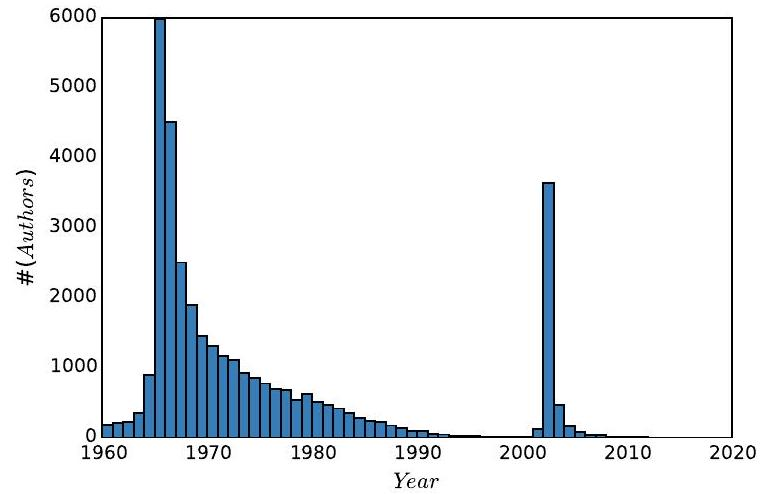
\includegraphics[max width=\textwidth]{2025_03_17_ca60ec0bfd96dcf8e028g-087}
    \caption{What \textenglish{artifacts} \textenglish{can} \textenglish{you} \textenglish{find} \textenglish{in} \textenglish{this} \textenglish{time} series, \textenglish{counting} \textenglish{the} \textenglish{number} \textenglish{of} author's \textenglish{names} \textenglish{first} \textenglish{appearing} \textenglish{in} \textenglish{the} \textenglish{scientific} \textenglish{literature} \textenglish{each} year?}
    \label{fig:artifacts_time_series}
\end{figure}

प्रोसेसिंग आर्टिफैक्ट्स का पता लगाने की कुंजी "स्निफ टेस्ट" है, उत्पाद को इतनी करीब से जांचना ताकि कुछ खराब गंध आ सके। कुछ खराब आमतौर पर ऐसा होता है जो अप्रत्याशित या चौंकाने वाला होता है क्योंकि लोग स्वभाव से आशावादी होते हैं। चौंकाने वाली अवलोकन वे हैं जिनके लिए डेटा वैज्ञानिक जीते हैं। वास्तव में, ऐसे अंतर्दृष्टि वह प्राथमिक कारण होते हैं जो हम जो करते हैं उसे करते हैं। लेकिन मेरे अनुभव में, अधिकांश चौंकाते अंततः आर्टिफैक्ट्स साबित होते हैं, इसलिए हमें उन्हें संदेहपूर्ण दृष्टिकोण से देखना चाहिए।

फिगर\ref{fig:artifacts_time_series}एक प्रोजेक्ट के कंप्यूटेशनल परिणाम प्रस्तुत करता है जहाँ हमने वैज्ञानिक प्रकाशन की प्रक्रिया की जाँच की। यह उन 100,000 सबसे उत्पादक लेखकों की समय श्रृंखला दिखाता है, जिन्हें उनके पहले पेपर के प्रकाशन वर्ष के अनुसार \textenglish{Pubmed} में वर्गीकृत किया गया है, जो कि बायोमेडिकल साहित्य की एक लगभग संपूर्ण ग्रंथ सूची है।

इस आकृति का गहराई से अध्ययन करें, और देखें कि क्या आप कोई ऎसी कला खोज सकते हैं जिस पर टिप्पणी की जा सकती है। मैं कम से कम दो देख सकता हूँ। यदि आप समस्या के कारण का पता लगा सकते हैं, तो अतिरिक्त श्रेय दिया जाएगा।

कलाकृतियों को खोजने की कुंजी उन विसंगतियों को देखना है जो आपके द्वारा देखने की अपेक्षा के विपरीत होती हैं। \textit{क्या होना चाहिए} कुमारी लेखकों की संख्या का वितरण, और यह समय के साथ कैसे बदलना चाहिए? सबसे पहले, उन चीज़ों का पूर्व वितरण तैयार करें जिन्हें आप देखने की उम्मीद करते हैं, ताकि आप संभावित विसंगतियों का उसके खिलाफ सही ढंग से मूल्यांकन कर सकें।

मेरी अंतःप्रेरणा कहती है कि नए शीर्ष वैज्ञानिकों का वितरण काफी समान होना चाहिए क्योंकि हर नए स्नातक छात्र वर्ग के साथ नए तारे जन्म लेते हैं। मैं यह भी अनुमान लगाऊँगा कि जनसंख्या के विस्तार के साथ एक धीरे-धीरे ऊपर की ओर प्रवृत्ति हो सकती है, और अधिक लोग वैज्ञानिक समुदाय में शामिल होते हैं। लेकिन यही तो मैं चित्र\ref{fig:artifacts_time_series} में नहीं देखता। इसलिए कोशिश करें कि क्या विसंगतियाँ/संभावित कलाकृतियाँ हैं...

\begin{figure}[h]
    \centering
    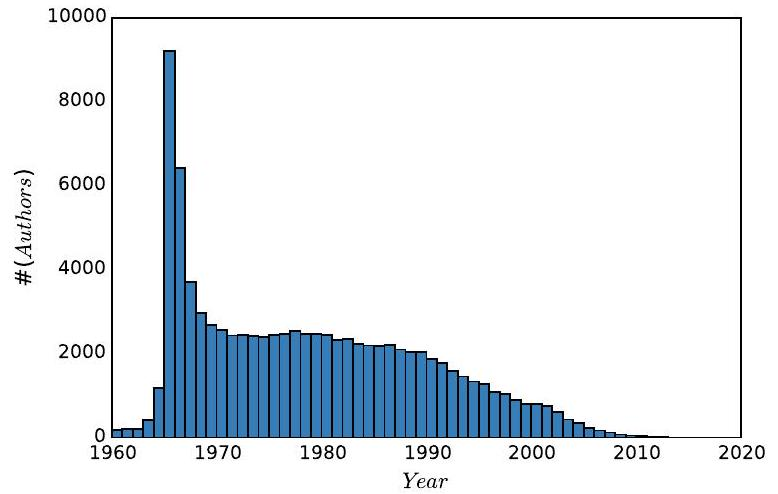
\includegraphics[max width=\textwidth]{2025_03_17_ca60ec0bfd96dcf8e028g-088}
    \caption{The \textenglish{cleaned} \textenglish{data} \textenglish{removes} \textenglish{these} artifacts, \textenglish{and} \textenglish{the} \textenglish{resulting} \textenglish{distribution} \textenglish{looks} correct.}
    \label{fig:cleaned_data}
\end{figure}

जब मैं चित्र\ref{fig:artifacts_time_series} को देखता हूँ, तो मुझे दो बड़े उभार दिखाई देते हैं: एक बायाँ उभार जो लगभग 1965 के आसपास शुरू होता है, और एक चोटी जो 2002 में विस्फोट करती है। थोड़ी सोच-विचार के बाद, बायाँ उभार समझ आता है। यह बाईं चोटी उस वर्ष होती है जब \textenglish{Pubmed} ने पहली बार नियमित रूप से ग्रंथ-सूची रिकॉर्ड को इकट्ठा करना शुरू किया। हालांकि 1960-1964 से कुछ बहुत ही अधूरे डेटा हैं, अधिकांश पुराने वैज्ञानिक जो कई वर्षों से पत्र प्रकाशित कर रहे थे, वे केवल 1965 में नियमित रिकॉर्ड के शुरू होने पर ही "उभर" सकते थे। इससे बाईं चोटी स्पष्ट होती है, जो फिर 1970 तक शान्त हो जाती है, और जो उस सपाट वितरण की तरह लगता है जिसकी हमने उम्मीद की थी।

लेकिन उस विशाल 2002 के शिखर के बारे में क्या? और नए लेखकों की संख्या में गिरावट जो इसके पहले वाले वर्षों में लगभग शून्य तक पहुँच जाती है? बड़े शिखर के दाईं ओर भी एक समान गिरावट दिखाई देती है। क्या 2002 में दुनिया के सभी प्रमुख वैज्ञानिकों का जन्म होना तय था?

बड़े पीक में रिकॉर्ड्स की सावधानीपूर्वक जांच से विसंगति का स्रोत पता चला: पहले नाम। प्रारंभिक दिनों में \textenglish{Pubmed} में लेखकों की पहचान उनके नाम के आद्याक्षर और अंतिम नाम द्वारा की जाती थी। लेकिन 2001 के अंत में, \textit{एसएस स्किएना} \textit{स्टीवन एस. स्किएना} बन गए, इसलिए यह \textit{दिखाई} देने लगा जैसे कोई नया लेखक स्वर्ग से उभर रहा हो।

लेकिन इस शिखर के बाएँ और दाएँ शून्यता की ओर गिरावट क्यों होती है? याद रखें कि हमने इस अध्ययन को 100,000 सबसे ज्यादा प्रकाशित वैज्ञानिकों तक सीमित किया है। यदि कोई वैज्ञानिक सितारा 1998 में उभरता है, तो वह शायद इस रैंकिंग में नहीं आ पाएगा क्योंकि कुछ साल बाद उनका नाम बदलने की संभावना थी, जिससे उन्हें अपने पूरे करियर के लेखों को संचित करने के लिए पर्याप्त समय नहीं मिलता। वितरण के बिलकुल दाएँ भी यही होता है: 2010 में नए बनाए गए वैज्ञानिक कभी भी केवल कुछ वर्षों में एक पूरे करियर का काम नहीं कर पाएंगे। दोनों घटनाओं को यह पहला नाम आधार सरलता से समझा देता है।\index{p-values}\index{permutation!tests}

इस डाटा को साफ करके नाम संदर्भों को एकीकृत करने में हमें इसे सही तरीके से करने के लिए कुछ पुनरावृत्तियाँ करनी पड़ीं। 2002 के शिखर को समाप्त करने के बाद भी, हमने देखा कि प्रमुख वैज्ञानिकों के अपने करियर शुरू करने में मध्य-1990 के दशक में एक महत्वपूर्ण गिरावट आई। यह इसलिए था क्योंकि कई लोग जिनका एक शानदार आधा करियर पहले नामों से पहले था और दूसरा शानदार आधा करियर पहले नामों के बाद, वे एक बड़ी संपूर्ण करियर की सीमा तक नहीं पहुँचे।

%---- \textenglish{Page} \textenglish{End} \textenglish{Break} \textenglish{Here} ---- \textenglish{Page} : 71

एकल अवधि में। इस प्रकार हमें यह तय करने के लिए सभी नामों को मिलाना पड़ा\textit{पहले}कि शीर्ष 100,000 वैज्ञानिक कौन थे।

चित्र 3.3 में हमारे लेखकों का अंतिम वितरण दिखाया गया है, जो हमारे अपेक्षित वितरण के प्लैटोनिक आदर्श से मेल खाता है। अपने डेटा के कंप्यूटर से निकलते ही उसे अविलंब तर्कसंगत बनाने में जल्दी मत करिए। मेरे सहयोगी एक समय पर 2002 के उभार को अनुसंधान फंडिंग में वृद्धि या नए वैज्ञानिक जर्नल्स की रचना के कारण दूर करने के लिए तैयार थे। हमेशा इस बात पर संदेह बनाए रखें कि आपका डेटा इतना साफ है कि उस पर भरोसा किया जा सके।

\subsection{डाटा कम्पैटिबिलिटी} हम कहते हैं कि दो वस्तुओं की तुलना "सेब से सेब" तब होती है जब यह एक निष्पक्ष तुलना होती है, यानी वस्तुएं इतनी समान होती हैं कि उन्हें एक दूसरे के खिलाफ सार्थक रूप से खड़ा किया जा सकता है। इसके विपरीत, "सेब से संतरे" तुलनाएँ अंततः अर्थहीन होती हैं। उदाहरण के लिए:

\begin{itemize}
  \item यह कोई मतलब नहीं बनता है कि 123.5 का वजन 78.9 से तुलना करें, जब एक पाउंड में है और दूसरा किलोग्राम में।
  \item यह कोई मतलब नहीं बनता कि फ़िल्म की कमाई \textit{Gone \textenglish{with} \textenglish{the} Wind} की तुलना \textit{Avatar} से करें, क्योंकि 1939 के डॉलर 2009 के डॉलर की तुलना में 15.43 गुना अधिक मूल्यवान हैं।
  \item यह कोई मतलब नहीं बनता कि आज न्यूयॉर्क और लंदन में दोपहर के समय सोने की कीमत की तुलना करें, क्योंकि समय क्षेत्र में पांच घंटे का फर्क है और कीमतें घटनाओं के बीच में बदलाव के कारण प्रभावित होती हैं।
  \item यह कोई मतलब नहीं बनता कि \textenglish{Microsoft} का स्टॉक मूल्य 17 फरवरी 2003 को 18 फरवरी 2003 के साथ तुलना करें, क्योंकि बीच में 2-फॉर-1 स्टॉक स्प्लिट ने कीमत को आधा कर दिया है, लेकिन वास्तविक मूल्य में कोई बदलाव नहीं दर्शाता।
\end{itemize}

जब भी डेटा सेट्स को मर्ज किया जाता है, इस प्रकार की डेटा तुलनीयता समस्याएँ उत्पन्न होती हैं। यहाँ मैं आपको दिखाने की आशा करता हूँ कि ऐसी तुलनीयता समस्याएँ कितनी खतरनाक हो सकती हैं, ताकि आप यह समझ सकें कि इनके प्रति जागरूक रहना क्यों आवश्यक है। इसके अलावा, कुछ महत्वपूर्ण वर्गों की कन्वर्ज़न के लिए मैं इनसे निपटने के तरीकों की ओर इशारा करता हूँ।

\textit{घर ले जाने वाला सबक:} किसी भी डेटा सेट में काम करते समय उसके प्रत्येक फ़ील्ड के अर्थ की समीक्षा करें। यदि आप उसमें शामिल विषयों और माप की इकाइयों तक को नहीं समझते हैं, तो आप इसे समझदारी से उपयोग नहीं कर सकते।

\section{मात्रक रूपांतरण}
भौतिक प्रणालियों में अवलोकनों को मात्रात्मक रूप में व्यक्त करने के लिए मानक माप की इकाइयों की आवश्यकता होती है। दुर्भाग्य से समान कार्य क्षमता रखने वाले लेकिन आपस में असंगत माप प्रणालियाँ मौजूद हैं। मेरी 12 वर्षीय बेटी और मेरा दोनों का वजन लगभग 70 है, लेकिन एक का वजन पाउंड में है और दूसरे का किलोग्राम में।

कंप्यूटर प्रणालियों में गलत माप इकाइयाँ डालने से रॉकेट विस्फोट जैसी विनाशकारी घटनाएँ होती हैं। विशेष रूप से, नासा ने 23 सितंबर, 1999 को एक मेट्रिक-से-अंग्रेजी रूपांतरण मुद्दे के कारण मार्स क्लाइमेट ऑर्बिटर स्पेस मिशन में \$125 मिलियन खो दिए।

ऐसी समस्याओं का सर्वोत्तम समाधान एकल मापन प्रणाली का चयन करना और उसी का पालन करना है। मेट्रिक प्रणाली पारंपरिक अंग्रेजी प्रणाली की तुलना में कई लाभ प्रदान करती है। विशेष रूप से, व्यक्तिगत माप स्वाभाविक रूप से एकल दशमलव मात्राओं के रूप में व्यक्त किए जाते हैं (जैसे 3.28 मीटर) बजाय असंगत जोड़ी मात्राओं के (5 फीट, 8 इंच)। यही समस्या कोणों (रेडियन बनाम डिग्री/सेकेंड) और वजन (किलोग्राम बनाम पाउंड/ऑज़) के मापन में भी आती है।\index{permutation!randomly generating}

मेट्रिक प्रणाली से चिपके रहना अपने आप में सभी तुलनात्मक मुद्दों का समाधान नहीं करता है, क्योंकि कुछ भी ऐसा नहीं है जो आपको मीटर और सेंटीमीटर में ऊँचाई मिश्रण करने से रोक सके। लेकिन यह एक अच्छी शुरुआत है।

आप अपने आप को असंगत यूनिट्स के खिलाफ कैसे सुरक्षित रख सकते हैं जब डेटा सेट्स को मिलाया जा रहा हो? सतर्कता आपका मुख्य हथियार होना चाहिए। सुनिश्चित करें कि आप अपने डेटा सेट में प्रत्येक संख्यात्मक स्तंभ के लिए निर्धारित यूनिट्स को जानते हैं, और मिलाते समय संगतता की जाँच करें। कोई भी स्तंभ जिसके पास एक संबंधित यूनिट या ऑब्जेक्ट प्रकार नहीं है, तुरंत संदिग्ध होना चाहिए।

जब विभिन्न स्रोतों से रिकॉर्ड मर्ज किए जा रहे हों, तो यह एक उत्कृष्ट प्रथा है कि एक नया "origin" या "source" फ़ील्ड बनाया जाए ताकि प्रत्येक रिकॉर्ड का स्रोत पहचाना जा सके। यह कम से कम इस आशा को प्रदान करता है कि इकाई परिवर्तन की गलतियों को बाद में सुधारा जा सकता है, समस्यापूर्ण स्रोत से रिकॉर्ड्स पर व्यवस्थित रूप से कार्य करके।

आंशिक रूप से स्वचालित प्रक्रिया को सांख्यिकीय महत्व परीक्षण से तैयार किया जा सकता है, जिसे खंड 5.3 में चर्चा की जाएगी। मान लीजिए कि हम मानव ऊंचाई की आवृत्तियों को अंग्रेजी (फीट) और मीट्रिक (मीटर) मापों के सम्मिलित डेटा सेट में प्लॉट करते हैं। हम वितरण में 1.8 के आसपास एक शिखर और 5.5 के आसपास दूसरा शिखर देखेंगे। वितरण में कई शिखरों का अस्तित्व हमें संदेहास्पद बना सकता है। दो इनपुट जनसंख्या पर महत्व परीक्षण से प्राप्त \textit{p}-मान यह दर्शाता है कि हमारे संदेह किस हद तक सही हैं।

\section{सांख्यिकीय प्रस्तुति रूपांतर}
सांख्यिकीय विशेषताएँ गणितीय मॉडलों में शामिल करने में सबसे आसान होती हैं। वास्तव में, कुछ मशीन लर्निंग ऐल्गोरिदम जैसे लाइनियर रिग्रेशन और सपोर्ट वेक्टर मशीन्स केवल सांख्यिकीय-संकेतनात्मक डेटा के साथ ही कार्य करते हैं। लेकिन यहाँ तक कि अंकों को अंकों में बदलने में भी एक सूक्ष्म समस्या हो सकती है। सांख्यिकीय क्षेत्रों को विभिन्न प्रकार से प्रस्तुत किया जा सकता है: पूर्णांक (123), दशमलव (123.5), या भिन्नों के रूप में (123 1/2)। अंकों को पाठ के रूप में भी प्रस्तुत किया जा सकता है, जिसके लिए "दस मिलियन" से 10000000 में सांख्यिकीय प्रसंस्करण के लिए परिवर्तन की आवश्यकता होती है।

संख्यात्मक प्रतिनिधित्व समस्याएँ एक और रॉकेट जहाज को नष्ट करने का श्रेय ले सकती हैं। एक आरीआन 5 रॉकेट को 4 जून, 1996 को \$500 मिलियन की लागत में प्रक्षेपित किया गया था, जो उड़ान भरने के चालीस सेकंड बाद विस्फोट हो गया, जिसका कारण अंततः 64-बिट फ्लोटिंग पॉइंट संख्या को 16-बिट पूर्णांक में परिवर्तित करने में असफलता के लिए मान्य गया।

पूर्णांकों और फ्लोटिंग पॉइंट (वास्तविक) संख्याओं के बीच अंतर बनाए रखना महत्वपूर्ण है। पूर्णांक गिनती की संख्याएँ हैं: मात्रा जो वास्तव में

%---- \textenglish{Page} \textenglish{End} \textenglish{Break} \textenglish{Here} ---- \textenglish{Page} : 73

% \textenglish{Page} : 73

डिस्क्रीट को पूर्णांकों के रूप में प्रदर्शित किया जाना चाहिए। भौतिक रूप से मापी गई मात्रा को कभी भी सटीक रूप से मापा नहीं जा सकता क्योंकि हम एक सतत् दुनिया में रहते हैं। इसलिए सभी मापनों को वास्तविक संख्याओं के रूप में रिपोर्ट किया जाना चाहिए। वास्तविक संख्याओं के पूर्णांक अनुमानों का उपयोग कभी-कभी स्थान बचाने के लिए गलत प्रयास में किया जाता है। ऐसा न करें: राउंडिंग या ट्रंकेशन के मात्रात्मक प्रभाव कलाकृतियों को प्रस्तुत करते हैं।

एक विशेष रूप से उलझे हुए डेटा सेट में, जिसका हमने सामना किया, शिशु के वजन को दो पूर्णांक क्षेत्रों (पाउंड और शेष आउंस) के रूप में प्रस्तुत किया गया था। उन्हें एकल दशमलव मात्रा में संयोजित करना कहीं बेहतर होता।

\section{नाम एकीकरण}
दो अलग-अलग डाटा सेट्स से रिकॉर्ड्स को एकीकृत करना तब संभव है जब वे एक सामान्य कुंजी फ़ील्ड साझा करते हैं। नाम अक्सर कुंजी फ़ील्ड्स के रूप में उपयोग किए जाते हैं, लेकिन उन्हें अक्सर असंगत रूप से रिपोर्ट किया जाता है। क्या\textit{José}वही व्यक्ति है जो\textit{Jose}है? कई अमेरिकी राज्यों के आधिकारिक जन्म रिकॉर्ड्स में ऐसे चिह्नों पर प्रतिबंध लगाया गया है, एक आक्रामक प्रयास के रूप में उन्हें संगत करने के लिए।

एक अन्य उदाहरण के रूप में, डेटाबेस मेरे प्रकाशनों को मेरे पहले (\textit{Steve}, \textit{Steven}, या \textit{S.}), मध्य (\textit{Sol}, \textit{S.}, या खाली), और अंतिम (\textit{Skiena}) नामों के काटेरियन उत्पाद के रूप में दिखाता है, जिससे नौ विभिन्न रूपांतर होते हैं। और स्थिति तब और बिगड़ जाती है जब हम वर्तनी की गलतियों को शामिल करते हैं। मैं खुद को गूगल पर \textit{Stephen} पहले नाम और \textit{Skienna} और \textit{Skeina} अंतिम नामों के साथ पा सकता हूँ।

कुंजियों द्वारा रिकॉर्ड्स को एकीकृत करना एक बहुत ही जटिल समस्या है, जिसका कोई जादुई समाधान नहीं है। यही कारण है कि आईडी नंबरों का आविष्कार हुआ था, इसलिए यदि संभव हो तो उन्हें कुंजियों के रूप में उपयोग करें।

सबसे अच्छी सामान्य तकनीक है एकीकरण: प्रत्येक नाम को एक एकल मानक संस्करण में बदलने के लिए साधारण पाठ रूपांतरण करना। सभी स्ट्रिंग्स को छोटे अक्षरों में बदलना (आमतौर पर सही) टक्करों की संख्या बढ़ाता है। मध्य नामों को समाप्त करना या कम से कम उन्हें संक्षेप में बदलने से और भी अधिक नाम मिलान/टक्करें होती हैं, जैसे कि पहले नामों को मानक संस्करणों में बदलना (जैसे कि सभी\textit{Steves}को\textit{Stevens}में बदलना)।

ऐसी कोई भी रूपांतर प्रक्रिया फ्रेंकनस्टीन-लोगों को बनाने का जोखिम उठाती है, एकल रिकॉर्ड जो कई निकायों से इकट्ठे होते हैं। अनुप्रयोग भिन्न होते हैं इस बात में कि अधिक खतरा अथवा तो अत्यधिक आक्रामक तरीके से विलय करने में है या बहुत संकोचपूर्ण तरीके में। यह समझें कि आपका कार्य इस स्पेक्ट्रम पर कहां स्थित है और उसी के अनुसार कार्य करें।

डेटा सेट्स को मिलाने में एक महत्वपूर्ण चिंता का विषय है \textit{वर्ण कोड एकीकरण}। पाठ स्ट्रिंग्स में वर्णों को संख्यात्मक प्रतिनिधित्व सौंपा जाता है, जिसमें प्रतीकों और संख्याओं के बीच की मैपिंग को वर्ण कोड मानक द्वारा नियंत्रित किया जाता है। दुर्भाग्यवश, सामान्य उपयोग में कई अलग-अलग वर्ण कोड मानक होते हैं, जिसका अर्थ है कि आप किसी वेबपेज से जो डेटा स्क्रैप करते हैं वह उस वर्ण कोड में नहीं हो सकता जिसे वह प्रणाली मानती है जो इसे प्रोसेस करेगी।

ऐतिहासिक रूप से, पुराने अच्छे 7-बिट\textit{एएससीआईआई}कोड मानक को 8-बिट\textit{आईएसओ 8859-1 लाटिन}वर्णमाला कोड में विस्तारित किया गया, जो कई यूरोपीय भाषाओं से वर्ण और विराम चिह्न जोड़ता है।\textit{यूटीएफ-8}यूनिकोड वर्णों के सभी कोडिंग का एक एन्कोडिंग है जो परिवर्तनीय संख्या के 8-बिट ब्लॉकों का उपयोग करता है, जो एएससीआईआई के साथ पिछड़े संगत है। यह वेब-पृष्ठों के लिए प्रमुख एन्कोडिंग है, हालांकि अन्य सिस्टम उपयोग में बने रहते हैं।

% \textenglish{Page} : 74

सही तरीके से संख्यात्मक कोड्स को मर्ज करने के बाद एकीकृत करना लगभग असंभव है। आपको एक मानक के रूप में एकल कोड चुनने की अनुशासन होना चाहिए और प्रत्येक इनपुट फ़ाइल के एन्कोडिंग की जांच करनी चाहिए, इसे टारगेट में बदलना चाहिए उससे पहले अतिरिक्त काम करने से पहले।

\section{समय/तिथि एकीकरण}
डेटा/समय मार्क का उपयोग घटनाओं के सापेक्ष क्रम का अनुमान लगाने और घटनाओं को सापेक्ष समानता से समूहित करने के लिए किया जाता है। कई स्रोतों से घटनाओं के डेटा को एकीकृत करने के लिए सावधानीपूर्वक सफाई की आवश्यकता होती है ताकि अर्थपूर्ण परिणाम सुनिश्चित किए जा सकें।

सबसे पहले हम समय मापने में आने वाली समस्याओं पर विचार करें। दो कंप्यूटरों की घड़ियां कभी भी पूरी तरह से समान नहीं होतीं, इसलिए विभिन्न प्रणालियों से लॉग्स को सटीकता से संरेखित करने के लिए काम और अनुमान दोनों की जरूरत होती है। विभिन्न क्षेत्रों से डेटा के मामले में समय क्षेत्र की समस्याएं भी होती हैं, और साथ ही दिन की रोशनी बचाने के समय में बदलाव के स्थानीय नियमों में विभिन्नताएं भी होती हैं।

सही उत्तर यहाँ है कि सभी समय मापनों को \textit{समन्वित सार्वभौमिक समय} (\textenglish{UTC}) के साथ संरेखित किया जाए, जो पारंपरिक \textit{ग्रीनविच मीन टाइम} (\textenglish{GMT}) को शामिल करने वाला एक आधुनिक मानक है। एक संबंधित मानक है \textit{यूनिक्स समय}, \index{UNIX time} जो गुरुवार, 1 जनवरी, 1970 को 00:00:00 \textenglish{UTC} से बीते हुए सेकंडों की संख्या के संदर्भ में एक घटना के सटीक समय का विवरण देता है।

ग्रेगोरियन कैलेंडर प्रौद्योगिकी जगत में सामान्य है, यद्यपि कई अन्य कैलेंडर प्रणालियाँ विभिन्न देशों में उपयोग में हैं। कैलेंडर प्रणालियों के बीच परिवर्तित करने के लिए सूक्ष्म एल्गोरिदम का उपयोग किया जाना चाहिए, जैसा कि \cite{reingold2001calendrical} में वर्णित है। तारीख संरेखण के लिए एक बड़ा मुद्दा समय क्षेत्रों और अंतर्राष्ट्रीय तारीख रेखा की उचित व्याख्या से संबंधित है।

समय श्रृंखला एकीकरण प्रायः व्यवसायिक कैलेंडर की प्रकृति के कारण जटिल होता है। वित्तीय बाजार सप्ताहांत और छुट्टियों पर बंद रहते हैं, जिससे व्याख्या की समस्याएँ उत्पन्न होती हैं जब आप, उदाहरण के लिए, स्टॉक की कीमतों को स्थानीय तापमान से जोड़ रहे होते हैं। सप्ताहांत में किस समय पर तापमान मापना सही होगा ताकि सप्ताह के अन्य दिनों के साथ संगति बनी रहे? \textenglish{Python} जैसी भाषाओं में वित्तीय समय श्रृंखला डेटा से निपटने के लिए व्यापक पुस्तकालय शामिल होते हैं ताकि इस तरह के मुद्दों को सही किया जा सके। इसी प्रकार की समस्याएँ मासिक डेटा के साथ भी उत्पन्न होती हैं, क्योंकि महीने (और यहाँ तक कि वर्ष) की लंबाई अलग-अलग होती है।

\section{वित्तीय एकीकरण}
पैसा दुनिया को चलाता है, इसीलिए इतने सारे डेटा विज्ञान परियोजनाएँ वित्तीय समय श्रृंखला के इर्द-गिर्द घूमती हैं। लेकिन पैसा गंदा हो सकता है, इसलिए इस डेटा को साफ करने की आवश्यकता होती है।

यहाँ एक समस्या है\textit{मुद्रा परिवर्तन},\index{currency conversion} जो एक मानकीकृत वित्तीय इकाई का उपयोग करके अंतरराष्ट्रीय कीमतों का प्रतिनिधित्व करता है। मुद्रा विनिमय दरें एक दिन के भीतर कुछ प्रतिशत तक भिन्न हो सकती हैं, इसलिए कुछ अनुप्रयोगों को समय-संवेदनशील परिवर्तनों की आवश्यकता होती है। परिवर्तन दरें वास्तव में मानकीकृत नहीं होती हैं। विभिन्न बाजारों में अलग-अलग दरें और\textit{स्प्रेड्स} होंगे, जो खरीद और बिक्री कीमतों के बीच का अंतर होता है जो परिवर्तन की लागत को कवर करता है।

%---- \textenglish{Page} \textenglish{End} \textenglish{Break} \textenglish{Here} ---- \textenglish{Page} : 75



अन्य महत्वपूर्ण सुधार मुद्रास्फीति के लिए है।\textit{पैसे का समय मूल्य}का अर्थ है कि आज का एक डॉलर (आमतौर पर) एक साल बाद के डॉलर की तुलना में अधिक मूल्यवान होता है, और ब्याज दरें भविष्य के डॉलर को छूट देने का सही तरीका प्रदान करती हैं। मुद्रास्फीति दरों का अनुमान वस्तुओं की टोकरी पर कीमतों के परिवर्तनों का अनुसरण करके लगाया जाता है और समय के साथ एक डॉलर की क्रय शक्ति को मानकीकृत करने का तरीका प्रदान करती हैं।\index{data-driven}\index{exploratory \textenglish{data} analysis}\index{hypothesis driven}\index{new \textenglish{data} set}

गैर-महत्वपूर्ण अवधियों में एक मॉडल में बिना समायोजित कीमतों का उपयोग करना बस परेशानी को आमंत्रित करने जैसा है। मेरे छात्रों के एक समूह ने एक बार शेयर कीमतों और तेल कीमतों के बीच तीस साल की अवधि में देखी गई मजबूत सहसंबंध से बहुत उत्साहित हो गए, और इसलिए एक वस्तु भविष्यवाणी मॉडल में शेयर कीमतों का उपयोग करने की कोशिश की। लेकिन दोनों वस्तुएं डॉलर में कीमत वाली थीं, बिना किसी समायोजन के जब वे मुद्रास्फीत हुई। मूलतः \textit{किसी भी} जोड़ी के वस्तुओं की कीमतों की समय श्रृंखला मुद्रास्फीति के लिए समायोजन नहीं करने पर समय के साथ मजबूत सहसंबंध दिखाएगी।\index{summary statistics}

वास्तव में, समय के साथ मूल्य परिवर्तन को दर्शाने का सबसे सार्थक तरीका संभवतः अंतर नहीं बल्कि \textit{प्रतिदान} है, जो आरंभिक मूल्य द्वारा अंतर को सामान्यीकृत करता है:

\[
r_{i}=\frac{p_{i+1}-p_{i}}{p_{i}}
\]

यह प्रतिशत परिवर्तन के समान अधिक है, यहाँ लाभ यह है कि इस अनुपात के लघुगणक को लेने पर यह लाभ और हानि के लिए सममिति हो जाता है।

वित्तीय समय श्रृंखलाओं में कई अन्य सूक्ष्मताएँ होती हैं जिन्हें सफाई की आवश्यकता होती है। कई स्टॉक्स शेयरधारकों को हर साल एक विशेष तारीख पर निर्धारित\textit{डिविडेंड्स}देते हैं। उदाहरण के लिए, मान लें कि माइक्रोसॉफ्ट 16 जनवरी को a\$2.50 डिविडेंड देगा। यदि उस दिन के शुरुआत में आपके पास माइक्रोसॉफ्ट का एक शेयर है, तो आपको यह चेक मिलेगा, इसलिए शेयर का मूल्य तुरंत a\$2.50 से घट जाता है जैसे ही डिविडेंड जारी किया जाता है। यह मूल्य गिरावट शेयरधारक के लिए कोई वास्तविक हानि नहीं दर्शाती है, लेकिन सही ढंग से साफ किया गया डेटा डिविडेंड को स्टॉक की कीमत में समायोजित करता है। यह कल्पना करना आसान है कि बिना सुधारित मूल्य डेटा पर प्रशिक्षित मॉडल डिविडेंड जारी करने से ठीक पहले स्टॉक्स बेचने के लिए सीख जाए, और ऐसा करने के लिए खुद पर अनुचित गर्व महसूस करे।

\subsection{गायब मानों का निपटान}

सभी डेटा सेट पूर्ण नहीं होते। डेटा की सफाई का एक महत्वपूर्ण पहलू उन फ़ील्ड्स को पहचानना है जिनके लिए डेटा उपलब्ध नहीं है, और फिर उनके लिए सही तरीके से तैयारी करना:

\begin{itemize}
  \item एक जीवित व्यक्ति की मृत्यु का वर्ष क्या है?
  \item खाली छोड़े गए सर्वेक्षण प्रश्न या ऐसे सवाल जिनमें स्पष्ट रूप से बेतुकी मूल्य भरी गई है, का क्या करना चाहिए?
  \item सीमित आकार के नमूने में दुर्लभ घटनाओं की सापेक्ष आवृत्ति क्या है?
\end{itemize}

संख्यात्मक डेटा सेट प्रत्येक मैट्रिक्स तत्व के लिए एक मान की उम्मीद करते हैं। गुम मान को शून्य पर सेट करना आकर्षक होता है, लेकिन आमतौर पर गलत होता है, क्योंकि इन मानों को डेटा के रूप में माना जाना चाहिए या नहीं, इस पर हमेशा कुछ अस्पष्टता होती है।

क्या किसी का वेतन शून्य है क्योंकि वह बेरोजगार है, या उसने बस सवाल का जवाब नहीं दिया?

बकवास मूल्यों का उपयोग गैर-डेटा प्रतीक के रूप में करने का खतरा यह है कि उन्हें मॉडल बनाने के समय डेटा के रूप में गलत समझा जा सकता है। आयु, शिक्षा, और लिंग से वेतन की भविष्यवाणी करने के लिए प्रशिक्षित एक रैखिक प्रतिगमन मॉडल उन लोगों के साथ समस्या में आ सकता है जिन्होंने प्रश्न का उत्तर देने से मना कर दिया।

किसी प्रतीक के रूप में$-1$का उपयोग करने में शून्य के समान ही कमियाँ हैं। वास्तव में, उस गणितज्ञ की तरह बनें जो ऋणात्मक संख्याओं से डरता है: उन्हें टालने के लिए किसी भी हद तक जाएँ।

\textit{घर ले जाने वाला सबक}: कच्चे डेटा और उसके साफ किए गए संस्करण को अलग-अलग बनाए रखें। कच्चा डेटा वास्तविकता की बुनियाद है, और इसे भविष्य के विश्लेषण के लिए वैसे का वैसा बनाए रखना चाहिए। साफ किया गया डेटा अनुमान के लिए गायब मानों को भरने के लिए इम्पुटेशन का उपयोग करके बेहतर हो सकता है। लेकिन कच्चा डेटा साफ किए गए डेटा से अलग रहे, ताकि हम अनुमान लगाने के विभिन्न तरीकों की जाँच कर सकें।\index{Anscombe’s Quartet}\index{summary statistics}

तो हम लापता मानों से कैसे निपटें? सबसे सरल तरीका यह है कि सभी रेकॉर्ड्स को छोड़ दें जिनमें लापता मान होते हैं। यह तरीका तब तक ठीक काम करता है जब तक यह पर्याप्त प्रशिक्षण डेटा छोड़ता है, बशर्ते कि लापता मान गैर-प्रणालीगत कारणों से अनुपस्थित हों। यदि जो लोग अपनी वेतन को बताने से इंकार कर रहे हैं, वे सामान्यतः औसत से ऊपर हैं, तो इन रेकॉर्ड्स को छोड़ने से पक्षपाती परिणाम मिलेंगे।

लेकिन आमतौर पर हम उन रेकॉर्ड्स का उपयोग करना चाहते हैं जिनमें कुछ क्षेत्र अनुपलब्ध हैं। इसे खाली छोड़ने के बजाय इसका अनुमान लगाना या\textit{अनुमानित करना}बेहतर हो सकता है। हमें अनुपलब्ध मानों को भरने के लिए सामान्य विधियों की आवश्यकता है। जिनमें शामिल हैं:

\begin{itemize}
\item \textit{ह्यूरिस्टिक-आधारित इंपुटैशन}:\index{IMDb!heuristic-based} यदि अंतर्निहित क्षेत्र का पर्याप्त ज्ञान उपलब्ध है, तो हमें कुछ क्षेत्रों के मान के लिए एक उचित अनुमान लगाने में सक्षम होना चाहिए। यदि मुझे उस वर्ष का मान भरने की आवश्यकता है जिसमें आप मरेंगे, तो \textit{जन्म वर्ष + 80} का अनुमान लगाना औसतन सही साबित होगा, और अंतिम उत्तर की प्रतीक्षा करने की तुलना में बहुत तेज होगा।\index{exploratory \textenglish{data} analysis!visualization}\index{visualization!tools}
\item \textit{मीन वैल्यू इंपुटैशन}: गायब मानों के लिए एक प्रॉक्सी के रूप में एक चर के मीन वैल्यू का उपयोग करना आमतौर पर समझदारी भरा होता है। पहले, मीन के साथ अधिक मान जोड़ने से मीन अपरिवर्तित रहता है, इसलिए हम अपने आँकड़ों को ऐसे इंपुटैशन द्वारा पक्षपाती नहीं करते हैं। दूसरे, मीन मान वाले क्षेत्र अधिकांश मॉडलों में एक सादा स्वाद जोड़ते हैं, इसलिए उनका डेटा का उपयोग करके बनाई गई किसी भी भविष्यवाणी पर मद्धम प्रभाव पड़ता है। 
\end{itemize}

लेकिन यदि डेटा गायब होने का कोई प्रणालीगत कारण है, तो औसत उपयुक्त नहीं हो सकता है। मान लीजिए कि हमने विकिपीडिया में औसत मृत्यु-वर्ष का उपयोग करके सभी जीवित लोगों के लिए गायब मान को अनुमानित किया। यह भयंकर साबित होगा, जिसमें कई लोगों को उनकी असल जन्म से पहले मरने के रूप में दर्ज किया जाएगा।

\begin{itemize}
  \item \textit{रैंडम वैल्यू इम्प्यूटेशन}: एक और दृष्टिकोण यह है कि कॉलम से एक रैंडम मान चुनें जो कि गायब मान की जगह ले ले। यह निश्चय ही खराब अनुमान का कारण बन सकता है, लेकिन असल में यही उद्देश्य है। बार-बार रैंडम मान चुनने से इम्प्यूटेशन के प्रभाव का सांख्यिकीय मूल्यांकन किया जा सकता है। अगर हम मॉडल को दस बार अलग-अलग इम्प्यूटेड\end{itemize}

%---- \textenglish{Page} \textenglish{End} \textenglish{Break} \textenglish{Here} ---- \textenglish{Page} : 77

% Mismatched: \sectionname{Dealing \textenglish{with} \textenglish{Missing} Values}

मान लें कि मान और परिणाम बहुत भिन्न-भिन्न होते हैं, तो हमें शायद मॉडल पर अधिक विश्वास नहीं करना चाहिए। यह सटीकता जांच विशेष रूप से मूल्यवान है जब डेटा सेट से बड़ा अंश गायब है।

\begin{itemize}
  \item \textit{निकटतम पड़ोसी द्वारा इम्पुटेशन}: क्या होगा अगर हम रिकॉर्ड की पहचान करें जो सभी उपस्थित फ़ील्ड पर सबसे करीब से मेल खाता है, और इस निकटतम पड़ोसी का उपयोग उन मानों को अनुमानित करने के लिए करें जो गायब हैं? जब रिकॉर्ड्स के बीच विचरण को समझाने के स्पष्ट कारण होते हैं, तो ऐसी भविष्यवाणियाँ औसत से अधिक सटीक होनी चाहिए।
\end{itemize}

इस दृष्टिकोण को समानतम रिकॉर्ड्स की पहचान करने के लिए दूरी फ़ंक्शन की आवश्यकता होती है।\textit{निकटतम पड़ोसी}विधियाँ डेटा विज्ञान में एक महत्वपूर्ण तकनीक हैं, और इन्हें अधिक विस्तार से खंड 10.2 में प्रस्तुत किया जाएगा।

\begin{itemize}
  \item \textit{इम्पुटेशन बाय इंटरपोलशन}: सामान्य रूप से, हम एक विधि जैसे कि रेखीय प्रतिगमन (धारा 9.1 देखें) का उपयोग करके लक्षित स्तंभ के मानों को भविष्यवाणी कर सकते हैं, जब दिए गए अन्य क्षेत्रों को रिकॉर्ड में देखा जाता है। ऐसे मॉडल्स को पूर्ण रिकॉर्ड्स पर प्रशिक्षित किया जा सकता है और फिर उन पर आवेदन किया जा सकता है जिनमें मान गायब हैं।\index{Tufte, Edward}\index{visualization aesthetic}\index{visualization aesthetic!chartjunk}\index{visualization aesthetic!data-ink ratio}\index{visualization aesthetic!lie factor}\index{visualization aesthetic!scaling \textenglish{and} labeling}
\end{itemize}

लिनियर रिग्रेशन का उपयोग करके गायब मानों की भविष्यवाणी करना तब सबसे अच्छा काम करता है जब प्रत्येक रिकॉर्ड में केवल एक फ़ील्ड गायब होती है। यहाँ संभावित खतरा है खराब भविष्यवाणियों के माध्यम से महत्वपूर्ण बाहरी मान निर्मित करना। रिग्रेशन मॉडल्स आसानी से एक अधूरी रिकॉर्ड को बाहरी मान में बदल सकते हैं, गायब फ़ील्ड्स को असामान्य रूप से उच्च या निम्न मूल्यों से भरकर। इससे डाउनस्ट्रीम विश्लेषण उन रिकॉर्ड्स पर अधिक ध्यान केंद्रित करेगा जिनमें गायब मान हैं, जो कि वास्तव में हम करना नहीं चाहते।

ऐसी चिंताएँ बाहरी तत्वों की पहचान के महत्व को उजागर करती हैं, जो कि सफाई प्रक्रिया का अंतिम चरण है जिसे यहाँ पर विचार किया जाएगा।

\subsection{बाह्य मान्यता पहचान}

डेटा संग्रह में हुई गलतियाँ आसानी से ऐसी \textit{विशेषताएँ} पैदा कर सकती हैं जो सही विश्लेषण में बाधा डाल सकती हैं। एक दिलचस्प उदाहरण अब तक की खोजे गए सबसे बड़े डायनासोर के कशेरुका से संबंधित है। 1500 मिलीमीटर की माप का यह अंग एक ऐसे व्यक्ति की संभावना को दर्शाता है जो 188 फीट लंबा था। यह आश्चर्यजनक है, विशेष रूप से क्योंकि अब तक खोजे गए ⸨दूसरे⸩ सबसे बड़े नमूने की लंबाई केवल 122 फीट है।

यहाँ सबसे संभावित व्याख्या (देखें \cite{goldenberg2016biggest}) यह है कि यह विशाल जीवाश्म वास्तव में कभी अस्तित्व में नहीं था: अमेरिकी प्राकृतिक इतिहास संग्रहालय से यह सौ वर्षों से अधिक समय से गायब है। शायद मूल माप एक सामान्य आकार की हड्डी पर लिया गया था और बीच के दो अंक गलती से बदले गए थे, जिससे कशेरुका की लंबाई 1050 मिलीमीटर तक घट गई।

डेटा एंट्री की गलतियों द्वारा अक्सर औट्लायर तत्व उत्पन्न होते हैं, जैसा कि यहाँ मामला प्रतीत होता है। ये स्क्रैपिंग में त्रुटियों से भी उत्पन्न हो सकते हैं, जैसे कि फॉर्मेटिंग में अनियमितता के कारण फुटनोट संख्या को संख्यात्मक मान के रूप में व्याख्यित किया जाना। केवल इसलिए कि कुछ लिखा हुआ है, उसे सही नहीं बनाता है। डायनोसोर उदाहरण की तरह, एक अकेला औट्लायर तत्व महत्वपूर्ण गलत व्याख्याओं की ओर ले जा सकता है।

सामान्य विवेकपूर्ण जाँच में प्रत्येक चर/स्तंभ में सबसे बड़े और सबसे छोटे मानों को देखना शामिल होता है ताकि यह पता लगाया जा सके कि वे बहुत अधिक विचलित तो नहीं हैं। यह सबसे अच्छे ढंग से आवृत्ति हिस्टोग्राम को प्लॉट करके और चरम तत्वों की स्थिति को देखकर किया जा सकता है। दृश्य निरीक्षण यह भी पुष्टि कर सकता है कि वितरण वैसा ही दिखता है जैसा उसे होना चाहिए, आमतौर पर घंटी के आकार का।

सामान्यतः वितरण किए गए डेटा में, यह संभावना कि एक मान औसत से$k$मानक विचलन पर है, $k$के साथ घातीय रूप से घटती है। यही कारण है कि 10 फीट ऊँचे बास्केटबॉल खिलाड़ी नहीं होते हैं, और यह बहिर्गामी पहचानने के लिए एक ठोस सीमा प्रदान करता है। पावर लॉ वितरणों में बहिर्गामी पहचानना इतना आसान नहीं होता है: वास्तव में \textit{एक}बिल गेट्स हैं जो औसत व्यक्ति से 10,000 गुना अधिक मूल्य रखते हैं।\index{lie factor}\index{visualization aesthetic!lie factor}

यह बहुत सरल है कि आउट्लायर क्षेत्रों को शामिल करने वाली पंक्तियों को मिटाकर आगे बढ़ जाएँ। आउट्लायर अक्सर अधिक प्रणालीगत समस्याओं की ओर संकेत करते हैं जिनसे निपटना होता है। जीवनकाल द्वारा ऐतिहासिक आंकड़ों के एक डेटा सेट पर विचार करें। बाइबल के मतूशलेह (969 वर्ष की आयु में) को आउट्लायर के रूप में पहचाना और उसे हटा देना आसान है।

लेकिन यह बेहतर है कि यह पता लगाया जाए कि क्या वह उन अन्य आंकड़ों का प्रतिनिधित्व करता है जिन्हें हमें हटाने पर विचार करना चाहिए। देखिए कि मथूसेलह की जन्म और मृत्यु तिथियाँ दृढ़ता से स्थापित नहीं थीं। शायद बिना तारीखों के किसी भी व्यक्ति की प्रकाशित उम्र को पर्याप्त शंकास्पद समझकर काट देना चाहिए। इसके विपरीत, विकिपीडिया में सबसे कम जीवनकाल वाले व्यक्ति (जॉन प्रथम, फ्रांस के राजा) ने केवल पांच दिन ही जिया। लेकिन 1316 में उसकी जन्म (15 नवंबर) और मृत्यु (20 नवंबर) तिथियाँ मुझे विश्वास दिलाती हैं कि उसका जीवनकाल सटीक था।

\section{युद्ध की कहानी: बाजार को मात देना}

हर बार जब हम मिले, मेरे स्नातकोत्तर छात्र वेनबिन ने मुझे बताया कि हम पैसा कमा रहे हैं। लेकिन हर बार जब मैंने पूछा, तो वह कम आत्मविश्वासी लग रहा था।

हमारी लिडिया सेंटीमेंट एनालिसिस प्रणाली ने समाचार और सोशल मीडिया के विशाल टेक्स्ट फ़ीड्स को लिया, उन्हें लाखों विभिन्न लोगों, स्थानों, और संगठनों के उल्लेख के लिए आवृत्ति और सेंटीमेंट की दैनिक समय श्रृंखला में बदल दिया। जब कोई व्यक्ति खेल चैंपियनशिप जीतता है, तो कई लेख लिखे जाते हैं जो यह विवरण देते हैं कि वह एथलीट कितने महान हैं। लेकिन जब यह खिलाड़ी फिर ड्रग के आरोप में पकड़ा जाता है, तो उनके बारे में लेखों का स्वर तुरंत बदल जाता है। सकारात्मक शब्दों (``विक्टोरियस'') और नकारात्मक शब्दों (``अरेस्टेड'') के साथ सह-संबंध की सापेक्ष आवृत्ति की गणना करके, हम किसी भी समाचार योग्य इकाई के लिए सेंटीमेंट संकेत बना सकते हैं।

वेनबिन ने अध्ययन किया कि भावना संकेतों का उपयोग भविष्य की घटनाओं की भविष्यवाणी करने के लिए कैसे किया जा सकता है, जैसे कि किसी विशेष फिल्म के लिए सकल कमाई, प्रकाशित समीक्षाओं या चर्चा की गुणवत्ता के प्रतिक्रिया स्वरूप। लेकिन वह विशेष रूप से इन डेटा का उपयोग स्टॉक मार्केट में खेलने के लिए करना चाहते थे।\index{stock market} स्टॉक्स ख़बरों के अनुसार ऊपर और नीचे जाते हैं। एक चूक गई आय रिपोर्ट किसी कंपनी के लिए बुरी ख़बर होती है, इसलिए कीमत नीचे जाती है। खाद्य और औषधि प्रशासन (\textenglish{FDA}) द्वारा किसी नई दवा की स्वीकृति उस कंपनी के लिए \textit{शानदार} खबर है जो इसे \textenglish{owns} करती है, इसलिए कीमत ऊपर जाती है। अगर वेनबिन हमारे भावना संकेत का उपयोग भविष्य की स्टॉक कीमतों की भविष्यवाणी करने के लिए कर सकते, तो चलो बस यह कहें कि मुझे अब उसे एक शोध सहायक के रूप में वेतन नहीं देना पड़ेगा।

इसलिए उसने उन शेयरों को खरीदने की रणनीति का अनुकरण किया जो सबसे उच्चतम

%---- \textenglish{Page} \textenglish{End} \textenglish{Break} \textenglish{Here} ---- \textenglish{Page} : 79

\section{भीड़-सोर्सिंग}
\index{crowdsourcing}\label{अनुभाग:भीड़-सोर्सिंग}

कोई भी व्यक्ति सभी उत्तर नहीं जानता। यहाँ तक कि मैं भी नहीं। बहुत सी बातें जो समझदारी के रूप में मानी जाती हैं, वे इस बात पर आधारित होती हैं कि हम विशेषज्ञता को कैसे एकत्रित करते हैं, और दूसरों के ज्ञान और अनुभव से राय कैसे बनाते हैं।

\begin{figure}[h!]
\centering
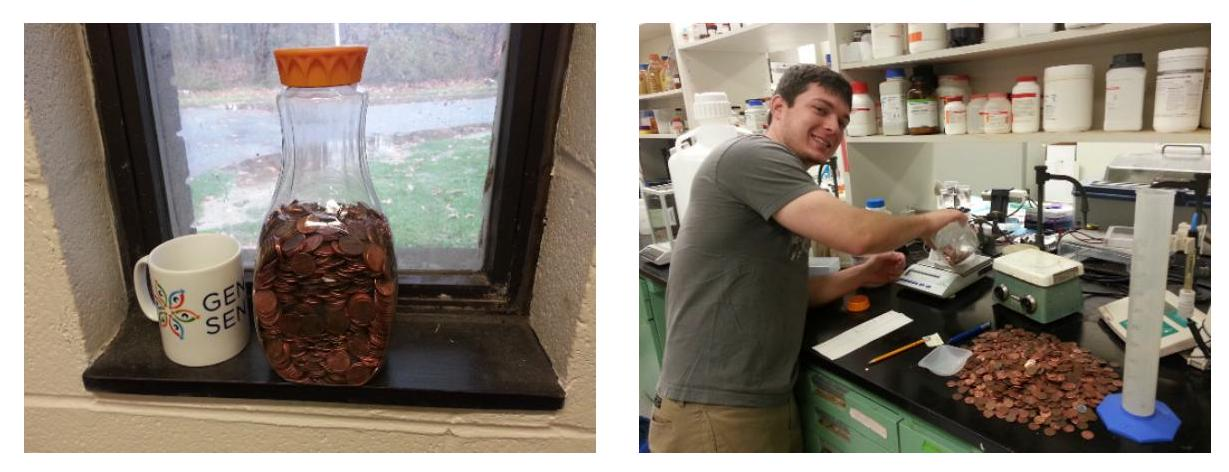
\includegraphics[max width=\textwidth]{2025_03_17_ca60ec0bfd96dcf8e028g-098}
\caption{Guess \textenglish{how} \textenglish{many} \textenglish{pennies} \textenglish{I} \textenglish{have} \textenglish{in} \textenglish{this} jar? (\textenglish{left}) \textenglish{The} \textenglish{correct} \textenglish{answer} \textenglish{was} \textenglish{determined} \textenglish{using} \textenglish{precise} \textenglish{scientific} \textenglish{methods} (\textenglish{right}).}
\label{fig:penny_jar}
\end{figure}

भीड़-स्रोतिंग बड़े संख्या में लोगों की अंतर्दृष्टि और श्रम को एक सामान्य लक्ष्य की ओर निर्देशित करती है। यह \textit{भीड़ की बुद्धि} का फायदा उठाती है, कि लोगों के समूह का सामूहिक ज्ञान संभवतः उनके बीच के सबसे समझदार व्यक्ति से भी अधिक हो सकता है।

यह धारणा एक बैल से शुरू हुई। फ्रांसिस गाल्टन, जो सांख्यिकी विज्ञान के संस्थापक और चार्ल्स डार्विन के रिश्तेदार थे, 1906 में एक स्थानीय पशु मेले में गए। उत्सवों के हिस्से के रूप में, गांववालों को इस विशेष बैल के वजन का अनुमान लगाने के लिए आमंत्रित किया गया, और जिस व्यक्ति का अनुमान सबसे करीब होगा उसे पुरस्कार मिलेगा। लगभग 800 प्रतिभागियों ने इसका अनुमान लगाया। किसी ने भी सही वजन 1,178 पाउंड नहीं चुना, फिर भी गाल्टन ने देखा कि औसत अनुमान आश्चर्यजनक रूप से करीब था: 1,179 पाउंड! गाल्टन के प्रयोग का सुझाव है कि कुछ कार्यों के लिए विशेषज्ञों से पूछने की बजाय विभिन्न व्यक्तियों के समूह को शामिल करके बेहतर परिणाम प्राप्त किए जा सकते हैं।

क्राउडसोर्सिंग मॉडलों के निर्माण में डेटा का एक महत्वपूर्ण स्रोत है, विशेष रूप से उन कार्यों के लिए जो मानव धारणा से संबंधित होते हैं। प्राकृतिक भाषा प्रोसेसिंग और कंप्यूटर दृष्टि में, मानव अभी भी स्टेट-ऑफ-द-आर्ट प्रणाली बने हुए हैं और सबसे उच्च स्तर का प्रदर्शन हासिल कर रहे हैं। प्रशिक्षण डेटा इकट्ठा करने का सबसे अच्छा तरीका अक्सर लोगों से किसी विशेष पाठ या छवि को स्कोर करने के लिए कहना होता है। पर्याप्त बड़े पैमाने पर यह करने के लिए, पर्याप्त मात्रा में प्रशिक्षण डेटा बनाने की आवश्यकता होती है, जिसमें बड़े संख्या में एनोटेटर्स, वास्तव में एक भीड़ की आवश्यकता होती है।

सोशल मीडिया और अन्य नई तकनीकों ने बड़े पैमाने पर रायों को एकत्रित और संकलित करना आसान बना दिया है। लेकिन हम भीड़ की बुद्धिमत्ता को शोरगुल से कैसे अलग कर सकते हैं?

\subsection{द पेनी डेमो}
\label{उप अनुभाग:पेनी डेमो}

चलो अपनी खुद की भीड़ की समझदारी के अनुभव के साथ शुरुआत करते हैं। तस्वीर\ref{fig:penny_jar}में एक जार की फोटो है जिसमें मैंने अपने ऑफिस में कई वर्षों के दौरान जमा किए गए पैसे हैं। इस जार में मेरे पास कितने पैसे हैं? अभी अपना अनुमान लगाओ, क्योंकि मैं आपको अगले पृष्ठ पर उत्तर बताने जा रहा हूँ।\index{visualization aesthetic!colors}\index{visualization aesthetic!repetition}

%---- \textenglish{Page} \textenglish{End} \textenglish{Break} \textenglish{Here} ---- \textenglish{Page} : 81

सही उत्तर प्राप्त करने के लिए, मैंने अपने जीवविज्ञानी-सहयोगी जस्टिन गार्डन को प्रिसीजन प्रयोगशाला के तराजू पर ये पेंसि तौलने को कहा। एक एकल पेंसि के वजन से भाग देकर संख्या प्राप्त होती है। जस्टिन को चित्र 3.4 (दाईं ओर) में अपने कार्य को लगन से करते हुए देखा जा सकता है।

तो मैं फिर से पूछता हूँ: आपके हिसाब से इस जार में कितने पैसे हैं? मैंने यह प्रयोग अपने डेटा साइंस क्लास के छात्रों पर किया। आपके जवाब की तुलना उनके जवाब से कैसे होगी?

मैंने पहले अपने ग्यारह छात्रों से कहा कि वे अपने विचार कार्डों पर लिखें और चुपचाप उन्हें कक्ष के सामने तक पहुंचा दें। इस प्रकार ये अनुमानों पूरी तरह से एक-दूसरे से स्वतंत्र थे। परिणाम, सुविधा के लिए छांटे गए, इस प्रकार थे:

\[
537, 556, 600, 636, 1200, 1250, 2350, 3000, 5000, 11,000, 15,000.
\]

फिर मैंने इन संख्याओं को बोर्ड पर लिखा और कुछ सांख्यिकी की गणना की। इन अनुमानों का माध्यिका 1250 था, जबकि औसत 3739 था। वास्तव में, इस जार में ठीक 1879 पैसे थे। मेरे छात्रों के बीच का माध्यिका स्कोर किसी भी एक अनुमान की तुलना में सही मात्रा के अधिक करीब था।

लेकिन वास्तविक कुल का खुलासा करने से पहले, मैंने एक और दर्जन छात्रों से अनुमान लगाने के लिए कहा। केवल अंतर यह था कि इस समूह ने बोर्ड पर लिखे गए पहले सेट के छात्रों के अनुमान देखे थे। उनके विकल्प थे: 
\[
750, 750, 1000, 1000, 1000, 1250, 1400, 1770, 1800, 3500, 4000, 5000। 
\]
इस समूह को अन्य लोगों के अनुमानों से अवगत कराने ने वितरण को मजबूत तरीके से प्रभावित किया, जिससे सभी बाहरी मान समाप्त हो गए: दूसरे समूह में न्यूनतम पहले चार अनुमानों से अधिक था, और अधिकतम पिछले दौर के तीन से कम या बराबर था। इस समूह के भीतर, माध्यिका 1325 थी और औसत 1935। दोनों ही वास्तविक उत्तर के कुछ हद तक करीब थे, लेकिन यह स्पष्ट है कि ग्रुप-विचार ने इसे संभव बनाने के लिए काम किया।

\textit{एंकरिंग} वह प्रसिद्ध संज्ञानात्मक पूर्वाग्रह है जिसमें लोगों के निर्णय पहले सुने गए संख्या पर अविवेकपूर्ण रूप से स्थिर हो जाते हैं। गाड़ी विक्रेता इसका हमेशा फायदा उठाते हैं, शुरुआत में वाहन की बढ़ी हुई कीमत बताकर ताकि बाद की कीमतें सौदे की तरह लगें।

मैंने फिर अंतिम परीक्षण किया उत्तर प्रकट करने से पहले। मैंने अपने छात्रों को बोली लगाने की अनुमति दी, जिसका अर्थ था कि उन्हें परिणाम पर पैसा लगाने के लिए पर्याप्त आत्मविश्वास होना चाहिए। इससे साहसी छात्रों की सिर्फ दो बोलियाँ आईं, क्रमशः 1500 और 2000 पैनी। मैंने उच्च बोली लगाने वाले से ₹1.21 कमाए, लेकिन दोनों बोली काफी करीब थीं। यह कोई आश्चर्य की बात नहीं है: जो लोग किसी घटना पर अपना पैसा दाँव पर लगाने के लिए तैयार होते हैं, वे, परिभाषा के अनुसार, अपनी पसंद में आत्मविश्वासी होते हैं।

\subsection{भीड़ कब समझदार होती है?}
जेम्स सुरोविकी के अनुसार उनकी पुस्तक\textit{द विज़डम ऑफ क्राउड्स}\cite{surowiecki2005wisdom} में, भीड़ तब समझदार होती है जब चार शर्तें पूरी होती हैं:

\begin{itemize}
\item \textit{जब राय स्वतंत्र होती हैं:} हमारे प्रयोग ने उजागर किया कि एक समूह कितनी आसानी से समूह-सोच में समा सकता है। लोग स्वाभाविक रूप से दूसरों से प्रभावित होते हैं। अगर आप किसी की सच्ची राय चाहते हैं, तो आपको उनको अलगाव में पूछना चाहिए।
\item \textit{जब भीड़ में विविध ज्ञान और विधियाँ होती हैं:} भीड़ केवल तब जानकारी जोड़ती है जब असहमति होती है। एक समिति जो पूरी तरह से-संक्रमित विशेषज्ञों से बनी हो, वह कुछ नया नहीं जोड़ती जो आप उनमें से किसी एक से सीख सकते थे। पेंस की अनुमानित समस्या में, कुछ लोगों ने कंटेनर की मात्रा का अनुमान लगाया, जबकि कुछ ने यह आंका कि जब मैंने भारी भार उठाया तो मेरे हाथ की ढलान कितनी हुई। अन्य दृष्टिकोण हो सकता है कि यह अनुमान लगाते कि बीस वर्षों में जब कभी-कभी मैंने अपनी जेबें खाली कीं तब मैं कितनी पेंस जमा कर सकता था, या अपनी खुद की जमा करने के अनुभवों को याद किया।
\item \textit{जब समस्या ऐसे क्षेत्र में होती है जिसे विशिष्ट ज्ञान की आवश्यकता नहीं होती:} मैं भीड़ की सहमति पर कुछ महत्वपूर्ण फ़ैसलों में भरोसा करता हूँ, जैसे कि किस प्रकार की कार खरीदनी चाहिए या मेरे देश का अध्यक्ष कौन होना चाहिए (गल्प)। लेकिन जब यह तय करने का सवाल हो कि मेरा ट्यूमर नमूना कैंसर का है या नहीं, तो मैं एक डॉक्टर के शब्द पर विश्वास करूंगा बजाय इसके कि फ़ोन बुक से रैंडमली चुने गए 1,000 नामों के समूह पर। क्यों? क्योंकि यह सवाल विशिष्ट ज्ञान और अनुभव से बहुत लाभान्वित होता है। इसमें एक सच्चा कारण है कि डॉक्टर \textit{जानना चाहिए} सभी दूसरों से अधिक। सरल दृष्टिगत कार्यों के लिए भीड़ का शासन है, लेकिन आपको सावधान रहना चाहिए कि भीड़ से कुछ ऐसा न पूछें जिसे वे जानने का कोई तरीका नहीं रखते।
\item \textit{रायों को उचित रूप से एकत्रित किया जा सकता है:} किसी भी बड़े सर्वेक्षण फॉर्म का सबसे कम उपयोगी हिस्सा है खुला प्रतिक्रिया फ़ील्ड "हमें बताएं कि आप क्या सोचते हैं!" समस्या यह है कि राय को एक सहमति में नहीं बदला जा सकता, क्योंकि अलग-अलग लोगों की अलग-अलग मुद्दे और चिंताएँ होती हैं। हो सकता है इन पाठों को समानता के आधार पर समूहों में रखा जा सकता है, लेकिन इसे प्रभावी रूप से करना कठिन है। ऐसे मुफ्त-फ़ॉर्म प्रतिक्रियाओं का सबसे सामान्य उपयोग गपशप के रूप में होता है। लोग सबसे सकारात्मक सुनाई देने वाली चुनते हैं, फिर उन्हें बॉस को प्रभावित करने के लिए स्लाइड पर लगाते हैं।
\end{itemize}

\textit{घर पर सीखें:} जीवन के आंशिक क्रम में एक असाधारण तत्व बनें। विविध, स्वतंत्र विचार भीड़ में सबसे अधिक ज्ञान का योगदान करते हैं।

\subsection{समुच्चयन की प्रक्रियाएँ}
उत्तरों के सेट से बुद्धिमत्ता संकलित करने के लिए सही समुच्चयन प्रक्रिया का उपयोग आवश्यक है। संख्यात्मक मात्राओं का अनुमान लगाने के लिए, आवृत्ति वितरण को प्लॉट करना और सारांश आँकड़े की गणना करना उपयुक्त होता है। औसत (\textenglish{mean}) और माध्यिका (\textenglish{median}) दोनों ही यह मानते हैं कि त्रुटियाँ

%---- \textenglish{Page} \textenglish{End} \textenglish{Break} \textenglish{Here} ---- \textenglish{Page} : 83

माध्यिका, सामान्य रूप से, इस तरह की संग्रहण समस्याओं में औसत से अधिक उपयुक्त विकल्प होती है। यह बहिर्गामी मानों के प्रभाव को कम करती है, जो विशेष रूप से उन मामलों में समस्या होती है जहाँ आपका कुछ प्रतिभागियों का प्रतिशत गलत हो सकता है। हमारे पेनी अनुमान डेटा पर, औसत ने 3739 का भयावह अधिक अनुमान उत्पन्न किया, जो सबसे बड़े और सबसे छोटे अनुमान को हटाए जाने के बाद 2843 हो गया, और फिर दोनों सिरों पर दो बहिर्गामी मानों को हटाने के बाद 2005 तक गिर गया (सही उत्तर 1879 था याद करें)।\index{box plots}\index{line charts!best practices}\index{uncertainty}\index{chart types!dot \textenglish{and} \textenglish{line} plots}\index{line charts}\index{line charts!advantages}

बहिष्कृतों को हटाना एक बहुत अच्छी रणनीति है, लेकिन हमारे विषयों की विश्वसनीयता का मूल्यांकन करने के लिए हमारे पास अन्य आधार भी हो सकते हैं, जैसे कि अन्य परीक्षणों में उनका प्रदर्शन जहां हम उत्तर जानते हैं। एक \textit{वेटेड एवरेज} लेना, जहां हम उन स्कोरों को अधिक महत्त्व देते हैं जिन्हें अधिक विश्वसनीय माना जाता है, हमें ऐसे विश्वास उपायों को ध्यान में रखने का तरीका प्रदान करता है।

वर्गीकरण समस्याओं के लिए, मतदान मौलिक एकत्रीकरण तंत्र है। \textit{कोंडोर्सेट जूरी प्रमेय} लोकतंत्र में हमारे विश्वास को उचित ठहराता है। यह बताता है कि यदि किसी दिए गए मुद्दे पर प्रत्येक मतदाता के सही होने की संभावना$p > 0.5$ है, तो बहुमत मतदाताओं के सही होने की संभावना\(P(\textenglish{n})\)\(p\) से अधिक है। वास्तव में, यह बिल्कुल है:

\[
P(\textenglish{n})=\sum_{i=(n+1) / 2}^{n}\binom{n}{i} p^{i}(1-p)^{n-i}
\]

बड़े मतदाता संख्या सांख्यिकीय रूप से मान्यता प्रदान करती है, यहां तक कि अत्यधिक विवादास्पद चुनावों को भी। मान लीजिए कि\(p=0.51\), जिसका अर्थ है कि सही पक्ष बस बहुमत में हैं। 101 सदस्यों वाली एक जूरी 57\% समय पर सही निर्णय तक पहुंचेगी, जबकि\(P(1001)=0.73\)और\(P(10001)=0.9999\)। सही निर्णय की संभावना 1 की ओर बढ़ती है जैसे ही\(n\rightarrow\infty\)।

चुनाव प्रणालियों की शक्ति के प्राकृतिक सीमाएँ होती हैं, हालांकि। \textit{एरो का असंभवता प्रमेय} यह दर्शाता है कि प्राथमिकताओं के क्रमचय को वोट के रूप में जोड़ने के लिए कोई भी चुनाव प्रणाली चुनाव की निष्पक्षता के चार प्राकृतिक शर्तों को पूरा नहीं करती है। इसे स्कोर और रैंकिंग के संदर्भ में अनुभाग 4.6 में चर्चा की जाएगी।

% Mismatched: \sectionname{Crowdsourcing Services}

क्राउडसोर्सिंग सेवाएँ जैसे \textenglish{Amazon} \textenglish{Turk} और \textenglish{CrowdFlower} आपको बड़ी संख्या में लोगों को छोटे-छोटे कार्य करने के लिए रखने का अवसर प्रदान करती हैं। वे आपको लोगों को व्यवस्थित करने में मदद करती हैं, ताकि आप अपने लिए डाटा बनाने के लिए लोगों को व्यवस्थित कर सकें।

ये भीड़-स्रोत सेवाएँ फ्रीलांस कामगारों के बड़े समूह को बनाए रखती हैं, जो उनके और संभावित नियोक्ताओं के बीच मध्यस्थ के रूप में कार्य करती हैं। इन कामगारों को आमतौर पर \textit{टरकर्स} कहा जाता है, जिन्हें उपलब्ध नौकरियों की सूची और उनके भुगतान की जानकारी दी जाती है, जैसा कि चित्र 3.5 में दिखाया गया है। नियोक्ताओं को आमतौर पर अपनी पसंद के स्थान और योग्यताओं के अनुसार कर्मचारियों को चुनने की कुछ क्षमता होती है, और यदि वे किसी कार्य को अधूरा मानते हैं तो वे बिना भुगतान के किसी कामगार के प्रयास को अस्वीकार करने की शक्ति रखते हैं। लेकिन नियोक्ताओं की स्वीकृति दर के आँकड़े प्रकाशित किए जाते हैं, और अच्छे कामगार अक्सर बुरे व्यवहार करने वालों के लिए काम नहीं करते हैं।

\begin{figure}[h]
    \centering
    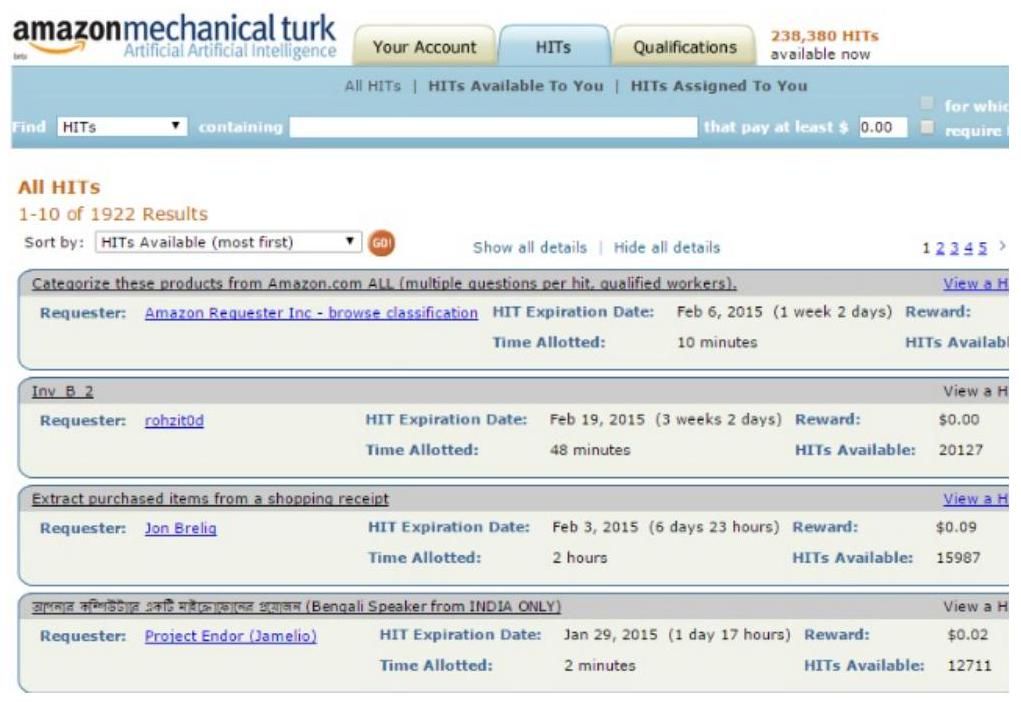
\includegraphics[max width=\textwidth]{2025_03_17_ca60ec0bfd96dcf8e028g-102}
    \caption{Representative \textenglish{tasks} \textenglish{on} \textenglish{Mechanical} Turk.}
\end{figure}

टर्कर्स को सौंपे गए कार्य सामान्यतः सरल संज्ञानात्मक प्रयासों से संबंधित होते हैं जिन्हें वर्तमान में कंप्यूटर द्वारा अच्छी तरह से नहीं किया जा सकता। टर्कर्स के अच्छे अनुप्रयोगों में शामिल हैं:

\begin{itemize}
  \item \textit{मानव धारणा के पहलुओं का मापन}: क्राउडसोर्सिंग प्रणालियाँ सरल कार्यों पर प्रतिनिधि राय एकत्रित करने के लिए प्रभावी तरीक़े प्रदान करती हैं। एक अच्छी एप्लिकेशन रंग-स्थान में लाल-हरा-नीला रंग के बीच संबंध स्थापित करना था, और उन नामों के बीच जो लोग आमतौर पर अपनी भाषा में इन रंगों को पहचानने के लिए प्रयोग करते हैं। यह तब महत्वपूर्ण होता है जब आप उत्पादों और छवियों का वर्णन लिख रहे होते हैं।\\\index{bar charts}\index{bubble plots}\index{chart types!bar charts}\index{chart types!pie charts}\index{pie charts}\index{scatter plots!three-dimensional}
  तो रंग स्थान में "नीला" और "हल्का नीला," या "रॉबिन्स एग ब्लू" और "टील" के बीच की सीमा कहाँ है? सही नाम संस्कृ्ति और परंपरा का कार्य होते हैं, भौतिकी का नहीं। यह जानने के लिए आपको लोगों से पूछना होता है, और क्राउडसोर्सिंग आपको सैकड़ों या हजारों अलग-अलग लोगों से आसानी से प्रश्न करने की अनुमति देता है।
  \item \textit{मशीन लर्निंग क्लासिफायरों के लिए प्रशिक्षण डेटा प्राप्त करना}: हमारी क्राउडसोर्सिंग में प्राथमिक रुचि मानव एनोटेशन का उत्पादन करना होगी जो प्रशिक्षण डेटा के रूप में कार्य करते हैं। कई मशीन लर्निंग समस्याएँ किसी विशेष कार्य को "जितना अच्छा लोग करते हैं" उतनी ही अच्छे से करने की कोशिश करती हैं। ऐसा करने के लिए यह आवश्यक है कि हमारे पास लोगों द्वारा किया गया कार्य किस तरह से किया गया था, यह स्थापित करने के लिए बड़ी संख्या में प्रशिक्षण उदाहरण हों।\\\index{heatmaps}
  उदाहरण के लिए, मान लीजिए कि हम एक सेंटीमेंट एनालिसिस सिस्टम बनाने का प्रयास कर रहे हैं जो लिखित समीक्षा को पढ़कर यह निर्णय ले सके कि उत्पाद की राय अनुकूल है या प्रतिकूल। हमें परीक्षक/प्रशिक्षण डेटा के रूप में काम करने के लिए एनोटेटर्स द्वारा लेबलित बड़ी संख्या में समीक्षाओं की आवश्यकता होगी। इसके अलावा, हमें एक ही समीक्षा को अलग-अलग एनोटेटर्स द्वारा बार-बार लेबल किया हुआ चाहिए, ताकि\end{itemize}

%---- \textenglish{Page} \textenglish{End} \textenglish{Break} \textenglish{Here} ---- \textenglish{Page} : 85

\begin{itemize}
  \item \textit{कंप्यूटर सिस्टम के लिए मूल्यांकन डेटा प्राप्त करना:} \textit{ए/बी परीक्षण} उपयोगकर्ता इंटरफेस को अनुकूलित करने के लिए एक मानक विधि है: न्यायाधीशों के आधे समूह को एक दिए गए सिस्टम का संस्करण \textit{A} दिखाएं और दूसरे आधे समूह को संस्करण \textit{B}। फिर यह परीक्षण करें कि कौन सा समूह किसी मीट्रिक के अनुसार बेहतर प्रदर्शन करता है। टर्कर्स यह प्रतिक्रिया दे सकते हैं कि एक दिए गए ऐप कितना दिलचस्प है, या एक नया वर्गीकारक कितना अच्छी तरह से प्रदर्शन कर रहा है।\\\index{bar charts!best practices}\index{bar charts!stacked}\index{pie charts!best practices}
मेरे एक ग्रेजुएट छात्र (यानक्विंग चेन) ने क्राउडफ्लावर का इस्तेमाल किया था एक सिस्टम के मूल्यांकन के लिए, जो किसी विशेष तत्व के लिए सबसे प्रासंगिक विकिपीडिया श्रेणी की पहचान करने के लिए बनाया गया था। कौन सी श्रेणी बराक ओबामा का बेहतर वर्णन करती है: \textit{संयुक्त राज्य के राष्ट्रपति} या \textit{अफ्रीकी-अमेरिकी लेखक}? \$200 में, उन्होंने कुल 10,000 इस तरह के बहु-विकल्प प्रश्नों का उत्तर प्राप्त किया, जो उनके सिस्टम के उचित मूल्यांकन के लिए पर्याप्त थे।
  \item \textit{मशीन में मनुष्यों को शामिल करना:} अभी भी कई संज्ञानात्मक कार्य मौजूद हैं जो लोग मशीनों से बेहतर करते हैं। एक चतुराई से डिज़ाइन किया गया इंटरफ़ेस उपयोगकर्ता क्वेरीज़ को कंप्यूटर के अंदर बैठने वालों को आपूर्ति कर सकता है, जो आवश्यकता में लोगों की मदद करने के लिए तैयार हैं।\\
मान लीजिए कि आप एक ऐसा ऐप बनाना चाहते हैं जो दृष्टिहीनों की मदद कर सके, जिससे उपयोगकर्ता को एक तस्वीर लेने और किसी से मदद माँगने की सुविधा मिले। शायद वे अपने रसोईघर में हैं, और उन्हें किसी से एक कैन का लेबल पढ़वाने की जरूरत है। यह ऐप एक टर्कर को एक उपरचना के रूप में बुला सकता है, ताकि जब इसकी आवश्यकता हो, तब ऐसा कार्य किया जा सके।\\
बेशक, इन छवि-व्याख्या जोड़ों को भविष्य के विश्लेषण के लिए संचित रखना चाहिए। ये मशीन लर्निंग प्रोग्राम के लिए ऐसे प्रशिक्षण डेटा के रूप में काम कर सकते हैं ताकि लोगों को जितना हो सके, इस प्रक्रिया से बाहर किया जा सके।
  \item \textit{स्वतंत्र रचनात्मक प्रयास:} क्राउडसोर्सिंग का उपयोग कई रचनात्मक कार्यों को मांग पर पूरा करने के लिए किया जा सकता है। आप मांग पर ब्लॉग पोस्ट या लेख ऑर्डर कर सकते हैं, या उत्पाद समीक्षाएं लिखवा सकते हैं, अच्छी या बुरी। जो कुछ भी आप कल्पना कर सकते हैं, बना सकते हैं, यदि आप बस यह निर्दिष्ट करें कि आप क्या चाहते हैं।\\
यहां दो मूर्खतापूर्ण उदाहरण हैं जिन्हें मैं किसी तरह प्रेरणादायक पाता हूँ:
    \begin{itemize}
      \item \textbf{द शीप मार्केट} (\href{http://www.thesheepmarket.com}{http://www.thesheepmarket.com}) के लिए प्रत्येक पाई के लिए 10,000 भेड़ों की ड्राइंग का आयोग बनाया गया। एक संकल्पना कला के टुकड़े के रूप में, यह उन्हें उच्चतम बोली लगाने वाले को बेचने की कोशिश करता है। आप किन रचनात्मक प्रयासों की कल्पना कर सकते हैं जो लोग आपके लिए \$0.25 प्रति बार में करेंगे?
      \item \textbf{इमोजी डिक} (\href{http://www.emojidick.com}{http://www.emojidick.com}) एक क्राउडसोर्स प्रयास था महान अमेरिकी उपन्यास \textit{मोबी डिक} को पूरी तरह से इमोजी छवियों में अनुवाद करने का। इसके निर्माताओं ने पुस्तक को लगभग 10,000 भागों में विभाजित किया, और प्रत्येक भाग को तीन अलग-अलग टर्करों द्वारा अनुवादित करवाया गया। अन्य टर्करों को इनमें से सबसे अच्छा चुनने के लिए काम पर रखा गया था ताकि उसे अंतिम पुस्तक में शामिल किया जा सके। 800 से अधिक टर्करों को शामिल किया गया, कुल \$3,676 की लागत के साथ जिसे क्राउड-फंडिंग साइट किकस्टार्टर द्वारा जुटाया गया।
    \end{itemize}

\item\textit{आर्थिक/मनोवैज्ञानिक प्रयोग:} भीड़-स्रोत ने व्यवहारिक अर्थशास्त्र और मनोविज्ञान में प्रयोग करने वाले सामाजिक वैज्ञानिकों के लिए एक वरदान साबित हुआ है। अपने अध्ययनों में स्थानीय स्नातकों को घूस देने की बजाय, ये अन्वेषक अब अपनी विषयों की संख्या को पूरे विश्व तक बढ़ा सकते हैं। उन्हें बड़ी जनसंख्या का उपयोग करने की शक्ति मिलती है, विभिन्न देशों में स्वतंत्र प्रतिकृतियाँ करने का अवसर मिलता है, और इस प्रकार अपनी परिकल्पनाओं के सांस्कृतिक पूर्वाग्रहों का परीक्षण कर सकते हैं।
\end{itemize}

भीड़-स्रोत का उपयोग करके कई रोमांचक कार्य लाभप्रद रूप से पूरे किए जा सकते हैं। हालाँकि, यदि आप गलत कार्य के लिए, गलत तरीके से टर्कर्स को नियुक्त करते हैं, तो आप निराशा के शिकार होने के लिए बाध्य हैं। भीड़-स्रोत के खराब उपयोगों में शामिल हैं:

\begin{itemize}
  \item \textit{किसी भी कार्य के लिए जिसमें उच्च प्रशिक्षण की आवश्यकता होती है:} हालांकि हर व्यक्ति के पास अद्वितीय कौशल और विशेषज्ञता होती है, क्राउडसोर्सिंग श्रमिकों के पास कोई विशेष प्रशिक्षण नहीं होता। उन्हें विनिमेय हिस्सों की तरह ट्रीट किया जाता है। आप इन श्रमिकों के साथ व्यक्तिगत संबंध स्थापित नहीं करते, और कोई भी समझदार गिग कुछ मिनटों के प्रशिक्षण से अधिक नहीं होगा।\\
विशिष्ट तकनीकी कौशल की आवश्यकता वाले कामों को क्राउडसोर्सिंग के माध्यम से करना उचित नहीं है। हालाँकि, इन्हें पारंपरिक लंबी अवधि की व्यवस्था में उचित तरीके से सब-ठेका किया जा सकता है।
  \item \textit{कोई भी काम जिसे आप स्पष्ट रूप से निर्दिष्ट नहीं कर सकते:} आपके पास टर्कर्स के साथ आगे-पीछे संचार के लिए कोई तंत्र नहीं होता। आम तौर पर, उनके पास आपसे सवाल पूछने का कोई तरीका नहीं है। इसलिए सिस्टम तभी काम करता है जब आप अपने काम को स्पष्ट, संक्षिप्त और अस्पष्टता से मुक्त कर सकते हों।\\
यह जितना दिखता है उससे कहीं कठिन है। समझें कि आप कंप्यूटर्स के बजाय लोगों को प्रोग्राम करने की कोशिश कर रहे हैं, जिसमें "जैसा मैं कहता हूँ वैसा करो" की बग्स "जो मैं कहना चाहता हूँ वैसा करो" को मात देती हैं। अपने लोकल लोगों पर अपनी स्पेसिफिकेशन्स की टेस्टिंग करें इससे पहले कि आप अपनी नौकरी को जनता के लिए खोलें, और फिर अपने क्राउडसोर्सिंग प्लेटफॉर्म पर इसका छोटा परीक्षण करें ताकि आप देख सकें कि यह कैसे चलता है इससे पहले कि आप अपने बजट के अधिकांश हिस्से को खर्च करने के लिए स्वतंत्र हो जाएं। आपको कुछ सांस्कृतिक आश्चर्य मिल सकते हैं। जो चीजें आपको स्पष्ट लगती हैं वे दुनिया के दूसरे छोर पर स्थित एक श्रमिक के लिए काफी अलग मायने रख सकती हैं।
  \item \textit{कोई भी काम जहाँ आप यह सत्यापित नहीं कर सकते कि वे अच्छा काम कर रहे हैं या नहीं:} टर्कर्स आपके पीसवर्क को लेने का एक ही उद्देश्य रखते हैं: वे अपने समय को यथासंभव कुशलता से पैसे में बदलना चाहते हैं। वे सबसे अच्छा पैसा पाने के लिए नौकरियां ढूंढते हैं, और सबसे चतुर लोग आपकी टास्क को यथासंभव जल्दी और बिना सोच के पूरा करने की कोशिश करेंगे।\\\index{chart types!data maps}\index{U.S. \textenglish{presidential} elections}
क्राउडसोर्सिंग प्लेटफॉर्म नियोक्ताओं को अनुबंधित काम अस्वीकार्य होने पर भुगतान रोकने की अनुमति देते हैं। इसका फायदा उठाने के लिए उत्पाद की गुणवत्ता को जांचने का कुछ कुशल तरीका होना आवश्यक है। शायद आपको उनसे कुछ कार्य करने के लिए कहना चाहिए जहाँ आपको पहले से सही उत्तर पता हो। शायद आप उनके उत्तरों की तुलना अन्य स्वतंत्र श्रमिकों के उत्तरों से कर सकते हैं, और यदि यह सहमति से बहुत कम बार सहमत होता है तो उनके कार्य को अस्वीकार कर सकते हैं।
\end{itemize}

%---- \textenglish{Page} \textenglish{End} \textenglish{Break} \textenglish{Here} ---- \textenglish{Page} : 87

\subsection{गेमिफिकेशन}\index{histograms!best practices}

यह बहुत महत्वपूर्ण है कि कुछ गुणवत्ता नियंत्रण प्रणाली को लागू किया जाए। किसी भी प्लेटफॉर्म पर उपलब्ध कामगारों का कुछ अंश बॉट्स होते हैं, जो यादृच्छिकता के माध्यम से बहुविकल्पीय कार्यों पर हमला करने की खोज में होते हैं। अन्य लोग ऐसे हो सकते हैं जिनमें दिए गए कार्य के लिए भाषा कौशल पूरी तरह से अप्र्याप्त हो सकते हैं। आपको इसे जांचना और अस्वीकार करना आवश्यक है ताकि आप ठगा न जाएं।

हालाँकि, आप खराब तरीके से निर्दिष्ट कार्यों से मिले परिणामों के बारे में उचित रूप से शिकायत नहीं कर सकते। बहुत अधिक अंश कार्य को अस्वीकार करने से आपकी प्रतिष्ठा, श्रमिकों और प्लेटफॉर्म के साथ, कम हो जाएगी। यह विशेष रूप से खराब कर्म है कि लोगों को भुगतान करने से इंकार करना लेकिन फिर भी उनके काम के उत्पाद का उपयोग करना।



शैक्षिक और अनुसंधान संस्थानों में लोग अपने \textit{संस्थागत समीक्षा बोर्ड} या \textenglish{IRB} के माध्यम से कानून से अधिक उच्च मानकों पर खरे उतरते हैं। \textenglish{IRB} शोधकर्ताओं और प्रशासनिक अधिकारियों की एक समिति है, जिसे मानव विषयों पर किसी भी शोध को शुरू करने से पहले अनुमोदित करना होता है। सौम्य क्राउडसोर्सिंग अनुप्रयोगों जैसे कि हमने चर्चा की है, को नियमित रूप से मंजूरी दी जाती है, उसके बाद शोधकर्ता एक छोटा ऑनलाइन प्रशिक्षण पाठ्यक्रम पूरा करते हैं ताकि वे नियमों को अच्छी तरह समझ सकें।\index{cartograms}\index{visualization!critiquing}

हमेशा यह समझें कि मशीन के दूसरी तरफ एक व्यक्ति है। उन्हें ऐसे काम न सौंपें जो अपमानजनक, नीचा दिखाने वाले, गोपनीयता का उल्लंघन करने वाले, या बहुत तनावपूर्ण हों। यदि आप अपने कर्मचारियों को इंसानों की तरह मानेंगे तो शायद आपको बेहतर परिणाम मिलेंगे।
\end{itemize}

लोगों से आपका काम करवाने के लिए सिर्फ स्पष्ट निर्देश नहीं बल्कि उचित प्रोत्साहन चाहिए। जीवन में, आमतौर पर आपको वही मिलता है जिसके लिए आप भुगतान करते हैं। अपने देश में वर्तमान में प्रचलित न्यूनतम घंटे की मजदूरी के बारे में जागरूक रहें, और अपने कार्यों की कीमत उसी के अनुसार तय करें। यह कोई कानूनी आवश्यकता नहीं है, लेकिन आमतौर पर यह अच्छा व्यापार होता है।

जो खतरनाक चमक $0.50 प्रति घंटे के हिसाब से श्रमिकों को काम पर रखने से आती है, वह जल्दी ही फीकी पड़ जाती है जब आप देखते हैं कि आपके कार्यों के लिए किस तरह के निम्न गुणवत्ता के श्रमिक आते हैं। आपके द्वारा उनकी कार्य उत्पाद को सख्ती से सुधारने की आवश्यकता के चलते आप अपनी सारी बचत आसानी से खर्च कर सकते हैं, शायद कई श्रमिकों को बार-बार इसे करने के लिए भुगतान करके। उच्चतर वेतन वाले कार्य श्रमिकों को बहुत जल्दी प्राप्त कर लेते हैं, इसलिए तैयार रहें इंतजार करने के लिए यदि आप प्रचलित दर का भुगतान नहीं करते हैं। बॉट्स और उनके कार्यात्मक समकक्ष कम वेतन स्वीकार करने में अधिक खुश होते हैं, जबकि आप वास्तव में जिन श्रमिकों को काम पर रखना चाहते हैं वे नहीं।



लोगों को अपनी डेटा को एनोटेट या ट्रांसक्राइब करने के लिए भुगतान करने का एक विकल्प है। इसके बजाय, चीजों को इतना मजेदार बनाइए कि लोग आपके लिए मुफ्त में काम करें!

\textit{उद्देश्य के साथ खेल}(\textenglish{GWAP}) ऐसे प्रणाली हैं जो डेटा संग्रहण को एक खेल के रूप में छिपाते हैं, जिसे लोग खेलना चाहते हैं, या एक कार्य जिसे लोग स्वयं करना चाहते हैं। खेल, उद्देश्य, और कल्पना के सही संयोजन के साथ, आश्चर्यजनक चीजें की जा सकती हैं। सफल उदाहरणों में शामिल हैं:



रीकैप्चा का आविष्कार हर दिन प्रदर्शित होने वाले 100 मिलियन से अधिक कैप्चा से उपयोगी डेटा प्राप्त करने के लिए किया गया था। प्रत्येक में दो पाठ स्ट्रिंग्स प्रदर्शित की जाती हैं, जिनमें से एक को सिस्टम द्वारा प्रवेश देने के लिए जांचा जाता है। दूसरा पुराने किताबों और अखबारों को डिजिटाइज़ करने वाले ओसीआर सिस्टम के लिए एक कठिन मामला दर्शाता है। उत्तरों को पुरालेखीय दस्तावेजों के डिजिटाइज़ेशन को सुधारने के लिए मैप किया जाता है, जिससे प्रति दिन 40 मिलियन से अधिक शब्दों का ट्रांसक्रिप्शन होता है।
    
\item\textit{खेलों/ऐप्स में मनोवैज्ञानिक/आईक्यू परीक्षण:}\index{IQ testing}मनोवैज्ञानिकों \index{psychologists}ने पाँच बुनियादी व्यक्तित्व लक्षणों को महत्वपूर्ण और पुनरुत्पादनीय व्यक्तित्व के पहलुओं के रूप में स्थापित किया है। शैक्षणिक मनोवैज्ञानिक व्यक्तिगत व्यक्तित्व पैमानों के साथ व्यक्तियों की स्थिति को मापने के लिए बहुविकल्पीय व्यक्तित्व परीक्षणों का उपयोग करते हैं, प्रत्येक बड़े पाँच लक्षणों के लिए: ओपननेस, कांशसनेस, एक्स्ट्रोवर्शन, एग्रीएबिलिटी, और न्यूरोटिसिज्म।

इन सर्वेक्षणों को गेम ऐप्स (“आपके \textit{व्यक्तित्व} के गुण कौन से हैं?”) में बदलकर मनोवैज्ञानिकों ने 75,000 से अधिक विभिन्न लोगों पर व्यक्तित्व माप एकत्रित किए हैं, साथ ही पसंदों और व्यवहार पर अन्य डेटा भी। इससे व्यक्तित्व के मनोविज्ञान में कई दिलचस्प मुद्दों का अध्ययन करने के लिए एक विशाल डेटा सेट तैयार हुआ है।

\item\textit{प्रोटीन संरचनाओं की भविष्यवाणी के लिए फोल्डइट गेम:}\index{FoldIt}प्रोटीन अणुओं द्वारा बनाई गई संरचनाओं की भविष्यवाणी करना विज्ञान में महान संगणकीय चुनौतियों में से एक है। कई सालों के काम के बावजूद, प्रोटीन को किसी विशेष आकार में मोड़ने वाला क्या है, यह अभी भी अच्छी तरह से समझा नहीं गया है।

फोल्डइट (\href{https://fold.it}{https://fold.it}) एक खेल है जो गैर-जीवविज्ञानियों को प्रोटीन अणुओं को डिज़ाइन करने की चुनौती देता है जो एक विशेष आकार में मोड़ते हैं। खिलाड़ियों को इस आधार पर स्कोर दिया जाता है कि उनका डिज़ाइन दिए गए लक्ष्य के कितने करीब आता है, और उच्चतम स्कोर करने वाले खिलाड़ियों को एक लीडर बोर्ड पर रैंक किया जाता है। विजेता डिज़ाइनों की ताकत पर कई वैज्ञानिक पत्र प्रकाशित किए जा चुके हैं।
\end{itemize}

यहां सफल होने की कुंजी एक ऐसा गेम बनाना है जो खेलने योग्य हो और लोकप्रिय बन सके। यह जितना प्रतीत होता है उससे कहीं अधिक कठिन है। ऍप स्टोर में लाखों मुफ्त ऍप्स उपलब्ध हैं, जिनमें अधिकांश गेम्स हैं। इनमें से बहुत कम ही ऐसे होते हैं जिन्हें कुछ सौ से अधिक लोग आजमाते हैं, जो डेटा संग्रहण के दृष्टिकोण से दिलचस्प होने के लिए कहीं भी पर्याप्त नहीं है। इस अतिरिक्त बाधा को जोड़ना कि गेम खेलते समय रोचक वैज्ञानिक डेटा उत्पन्न करे, इस कार्य को और भी कठिन बना देता है।

प्रेरणादायक तकनीकों का उपयोग खेलता को सुधारने के लिए किया जाना चाहिए। स्कोरिंग किसी भी खेल का एक महत्वपूर्ण हिस्सा है, और खेल को इस तरह से डिज़ाइन किया जाना चाहिए कि प्रदर्शन पहले तीव्रता से बढ़े, ताकि खिलाड़ी को आकर्षित किया जा सके। प्रगति बार...

%---- \textenglish{Page} \textenglish{End} \textenglish{Break} \textenglish{Here} ---- \textenglish{Page} : 89

\section{अध्याय नोट्स}

चार्ल्स बैबेज़ का उद्धरण जो इस अध्याय की शुरुआत में है, उनकी पुस्तक \textit{एक विचारक के जीवन के प्रसंग} से लिया गया है। मैं पदुआ का ग्राफिक उपन्यास \cite{babbage2011passages} की सिफारिश करता हूँ, जो उनके कार्य और एडा लोवलेस के साथ उनके संबंध का मनोरंजक लेकिन अर्थपूर्ण (हालाँकि काल्पनिक) परिचय देता है।

कई पुस्तकें विशेष प्रोग्रामिंग भाषाओं में डेटा प्रबंधन के व्यावहारिक मामलों से संबंधित हैं। विशेष रूप से उपयोगी हैं ओ'रिली पुस्तकें डेटा विज्ञान के लिए पाइथन में, जिनमें \cite{grus2015data}, \cite{mckinney2012python}.\index{Python} शामिल हैं।

हमारी जै-आलाइ शर्त प्रणाली की कहानी, जिसमें वेबसाइट स्क्रैपिंग की भूमिका शामिल है, मेरी किताब \textit{Calculated Bets}\cite{ski2001calculated} में रिपोर्ट की गई है। यह भविष्यवाणी के लिए सिमुलेशन मॉडलों को बनाने के तरीके का एक त्वरित और मजेदार अवलोकन है, और यह अनुभाग 7.8 की युद्ध कहानी का विषय होगा।

अंतरिक्ष अभियानों की विफलता को संख्यात्मक संगणना त्रुटियों के कारण लोकप्रिय मीडिया में अच्छी तरह से दस्तावेजीकृत किया गया है। अँतरिक्ष 5 और मंगल जलवायु ऑर्बिटर अंतरिक्ष अभियानों पर चर्चा के लिए ग्लीक \cite{gleick1996bug} और स्टीफेनसन एट अल. \cite{smb1999} देखें।

सेल फोन में एक्सेलेरोमीटर का उपयोग करके भूकंप का पता लगाने का चालाक विचार \textenglish{Faulkner} \textenglish{et} al. \cite{fch2014} से आता है। बड़े सेट्स के फ़्लिकर छवियों के प्रतिनिधि अध्ययन \textenglish{Kisilevich} \textenglish{et} al. \cite{kkk2010} शामिल हैं।

किटुर \textenglish{Report}  अमेज़ॅन टर्क पर \textenglish{crowdsourcing} उपयोगकर्ता अध्ययन अनुभवों पर रिपोर्ट करता है। ऐतिहासिक व्यक्तियों के उपयुक्त वर्णनों की पहचान के लिए हमारे द्वारा \textenglish{CrowdFlower} का उपयोग \cite{kittur2008crowdsourcing} में प्रस्तुत किया गया था। शिक्षण में कर्मचारियों को प्रोत्साहित करने के तरीकों पर चर्चा \cite{chen2015vector} में की गई है। \textenglish{Recaptchas} का परिचय वॉन अहेन एट अल \cite{deterding2011game, kapp2012gamification} में दिया गया है। मोबाइल ऐप्स के माध्यम से मनोवैज्ञानिक गुण डेटा का बड़े पैमाने पर संग्रह कोसिंस्की एट अल \cite{vamm2008} के कारण है।

\section{अभ्यास}

% Mismatched: \subsectionname{Data Munging}



\item [3-2.]\textit{[5]}प्रमुख डेटा साइंस प्रोग्रामिंग भाषाओं में से दो का चयन करें, और दोनों में निम्नलिखित कार्यों को हल करने के लिए प्रोग्राम लिखें। प्रत्येक कार्य के लिए आपको कौन सी भाषा सबसे उपयुक्त लगी?

\begin{enumerate}
        \item हेलो वर्ल्ड! 
        \item किसी फ़ाइल से संख्याएँ पढ़ें, और उन्हें क्रम में छपाएँ। 
        \item एक टेक्स्ट फ़ाइल पढ़ें, और शब्दों की कुल संख्या गिनें। 
        \item एक टेक्स्ट फ़ाइल पढ़ें, और \textit{अद्वितीय} शब्दों की कुल संख्या गिनें। 
        \item संख्याओं की एक फ़ाइल पढ़ें, और उनका आवृत्ति हिस्टोग्राम प्लॉट करें। 
        \item वेब से एक पेज डाउनलोड करें, और उसे स्क्रैप करें। 
    \end{enumerate}

\item [3-3.]\textit{[3]}थोड़ी देर के लिए Python, R, और \textenglish{Matlab} के साथ खेलें। आपको कौन सा सबसे अच्छा लगता है? प्रत्येक की ताकतें और कमजोरियाँ क्या हैं?

\item [3-4.]\textit{[5]}$n$मनुष्यों की ऊँचाई का एक डेटा सेट तैयार करें, जिसमें$p\%$उनका रिकॉर्ड अंग्रेज़ी (\textenglish{feet}) में और बाकी माप (\textenglish{meter}) में किया गया हो। सांख्यिकीय परीक्षणों का उपयोग करके परीक्षण करें कि क्या यह वितरण मीटर में सही तरीके से रिकॉर्ड किए गए डेटा से अलग है।$n$और$p$के रूप में सीमा क्या है जहाँ यह स्पष्ट हो जाता है कि कोई समस्या है?
\end{enumerate}

\subsection{डेटा स्रोत}



\item [3-6.]\textit{[5]} निम्नलिखित में से एक या अधिक\textit{द क्वांट शॉप} चुनौतियों के लिए, संबंधित डाटा स्रोत खोजें और उनकी गुणवत्ता का मूल्यांकन करें:

\begin{itemize}
        \item \textit{मिस यूनिवर्स.}
        \item \textit{मूवी ग्रॉस.}
        \item \textit{बेबी वेट.}
        \item \textit{आर्ट ऑक्शन प्राइस.}
        \item \textit{क्रिसमस पर बर्फ.}
        \item \textit{सुपर बाउल/कॉलेज चैंपियन.}
        \item \textit{घूल पूल?}
        \item \textit{भविष्य का गोल्ड/ऑइल प्राइस?}
    \end{itemize}

\end{enumerate}

\subsection{डाटा क्लीनिंग}



\item [3-8.]\textit{[3]}आप निम्नलिखित डेटा सेट्स में किस प्रकार के बहिर्वाहों के होने की उम्मीद कर सकते हैं:

\begin{enumerate}
        \item छात्र ग्रेड्स.
        \item वेतन डेटा.
        \item विकिपीडिया में जीवनकाल.
    \end{enumerate}

\item [3-9.]\textit{[३]} एक स्वास्थ सेंसर बीस विभिन्न मानों की एक धारा उत्पन्न करता है, जिसमें रक्तचाप, हृदय गति, और शरीर का तापमान शामिल हैं। उन दो या अधिक तकनीकों का वर्णन करें जिन्हें आप सेंसर से आने वाली डेटा धारा की वैधता की जांच के लिए उपयोग कर सकते हैं।
\end{enumerate}

\subsection{कार्यान्वयन परियोजनाएँ}



\item [3-11.]\textit{[5]}संयुक्त राज्य अमेरिका में मतदाता पंजीकरण रिकॉर्ड को नियंत्रित करने वाले कानून राज्य से राज्य में भिन्न होते हैं। एक या अधिक राज्यों की पहचान करें जिनके नियम बहुत ढीले हैं, और देखें कि डेटा प्राप्त करने के लिए आपको क्या करना होगा। संकेत: फ्लोरिडा।
\end{enumerate}

% Mismatched: \subsectionname{Crowdsourcing}



\item [3-13.]\textit{[3]}मान लें कि आप टेक्स्ट पढ़ने और उन्हें अंतर्निहित भावना (सकारात्मक या नकारात्मक) के आधार पर एनोटेट करने के लिए टरकर्स को भुगतान कर रहे हैं। यह एक विचारधारा से जुड़ा कार्य है, लेकिन हम कैसे एल्गोरित्मिक रूप से निर्धारित कर सकते हैं कि टरकर ने बेतरतीब या मनमाना ढंग से उत्तर नहीं दिए बल्कि अपना काम गंभीरता से किया?
\end{enumerate}

\subsection{साक्षात्कार प्रश्न}



\item [3-15.]\textit{[5]}सामान्य रूप से, आप अपवादों की पहचान कैसे करेंगे, और अगर आपको कोई मिलता है तो आपको क्या करना चाहिए?

\item [3-16.]\textit{[3]}डेटा क्लीनिंग विश्लेषण में महत्वपूर्ण भूमिका क्यों निभाता है?
\end{enumerate}

%---- \textenglish{Page} \textenglish{End} \textenglish{Break} \textenglish{Here} ---- \textenglish{Page} : 92
\textenglish{Here} \textenglish{is} \textenglish{the} \textenglish{LaTeX} \textenglish{content} \textenglish{formatted} \textenglish{according} \textenglish{to} \textenglish{the} \textenglish{JSON} \textenglish{data} \textenglish{and} \textenglish{guidelines} provided:



\begin{enumerate}
    \item[3-17.] \textit{[5]} विश्लेषण के दौरान, खोए हुए मानों का कैसे प्रबंधन करते हैं?
    \item[3-18.] \textit{[5]} चयन पूर्वाग्रह को समझाइए। यह क्यों महत्वपूर्ण है? डेटा प्रबंधन प्रक्रियाओं जैसे कि खोए हुए डेटा का प्रबंधन इसे कैसे खराब कर सकता है?
    \item[3-19.] \textit{[3]} वेब डेटा को कुशलतापूर्वक कैसे स्क्रैप करते हैं?
\end{enumerate}

% Mismatched: \sectionname{Kaggle Challenges}

\begin{enumerate}
    \item आंशिक रूप से धूप, हैशटैग की संभावना के साथ। \href{https://www.kaggle.com/c/crowdflower-weather-twitter}{\index{CrowdFlower}https://www.kaggle.com/c/crowdflower-weather-twitter}
    \item दिन के अंत में स्टॉक रिटर्न की भविष्यवाणी करें, बिना शोर से भ्रमित हुए। \\ \href{https://www.kaggle.com/c/the-winton-stock-market-challenge}{https://www.kaggle.com/c/the-winton-stock-market-challenge}
    \item डेटा सफाई और ऐतिहासिक जलवायु परिवर्तन का विश्लेषण। \\ \href{https://www.kaggle.com/berkeleyearth/climate-change-earth-surface-temperature-data}{https://www.kaggle.com/berkeleyearth/climate-change-earth-surface-temperature-data}
\end{enumerate}

\chapter{स्कोर्स और रैंकिंग्स}

पैसा एक स्कोरबोर्ड है जहाँ आप देख सकते हैं कि आप दूसरों के मुकाबले कैसे कर रहे हैं।

\begin{flushright}
  -- मार्क क्यूबन
\end{flushright}

\section{स्कोरिंग फ़ंक्शन का परिचय}

\textit{स्कोरिंग फंक्शन्स} वे मापदंड होते हैं जो बहु-आयामी रिकॉर्ड्स को एकल मान में परिवर्तित करते हैं, जिससे आँकड़ों की किसी विशेष विशेषता को उजागर किया जा सके। स्कोरिंग फंक्शन्स का एक परिचित उदाहरण वे होते हैं जो छात्रों को कोर्स में ग्रेड देने के लिए उपयोग किए जाते हैं, जैसे कि मेरे कोर्स में। छात्र फिर इन संख्यात्मक अंकों के अनुसार क्रमबद्ध (सॉर्ट) किए जा सकते हैं, और बाद में इस क्रम के आधार पर उनको अक्षर ग्रेड दिए जाते हैं।

ग्रेड्स को आमतौर पर संख्यात्मक विशेषताओं के ऊपर फंक्शन्स द्वारा मापा जाता है जो छात्र की प्रदर्शन को दर्शाते हैं, जैसे कि प्रत्येक गृहकार्य और परीक्षा पर प्राप्त अंकों के आधार पर। प्रत्येक छात्र को एकल संयुक्त स्कोर प्राप्त होता है, जिसे अक्सर 0 से 100 के बीच मापा जाता है। ये स्कोर आमतौर पर इनपुट वेरिएबल्स के एक रैखिक संयोजन से आते हैं, जैसे पांच गृहकार्य असाइनमेंट प्रत्येक को 8\% वजन दिया जाता है, और तीन परीक्षाओं में से प्रत्येक को 20\% वजन दिया जाता है।

ऐसे ग्रेडिंग रुब्रिक के बारे में कई बातें देखने लायक हैं, जिन्हें हम अधिक सामान्य स्कोरिंग और रैंकिंग फंक्शनों के मॉडल के रूप में उपयोग करेंगे:

\begin{itemize}
\item \textit{मनमानी का स्तर:} हर शिक्षक/प्रोफेसर अपने छात्रों का मूल्यांकन करते समय होमवर्क अंकों और परीक्षा अंकों के बीच अलग-अलग समझौते का उपयोग करते हैं। कुछ अंतिम परीक्षा को अन्य सभी चर से अधिक महत्व देते हैं। कुछ औसत निकालने से पहले प्रत्येक मूल्य को 100 पर सामान्यीकृत करते हैं, जबकि अन्य प्रत्येक स्कोर को एक Z-स्कोर में परिवर्तित करते हैं। उनकी दर्शन भिन्न होती है, फिर भी हर शिक्षक/प्रोफेसर यह निश्चित होता है कि उनका ग्रेडिंग सिस्टम काम करने का सबसे अच्छा तरीका है। 
\item \textit{मान्यकरण डेटा की कमी:} किसी भी "सही" ग्रेड के बारे में शिक्षकों को सूचनाएं देने वाला कोई स्वर्ण मानक नहीं है, जो उनके छात्रों को पाठ्यक्रम में प्राप्त होना चाहिए था। विद्यार्थी अक्सर शिकायत करते हैं कि मुझे उन्हें बेहतर ग्रेड देना चाहिए, लेकिन इन अनुरोधों के पीछे वस्तुनिष्ठता से अधिक स्वार्थ प्रतीत होता है। वास्तव में, मुझे शायद ही कभी छात्र यह सुझाव देते सुनाई देते हैं कि मैं उनका ग्रेड कम कर दूं। 
\item \textit{सामान्य मजबूती:} और फिर भी, व्यापक रूप से भिन्न और पूरी तरह से अप्रमाणित दृष्टिकोणों का उपयोग करने के बावजूद, विभिन्न ग्रेडिंग सिस्टम आम तौर पर समान परिणाम उत्पन्न करते हैं। हर स्कूल में \textenglish{A} श्रेणी के छात्र होते हैं जो हर कोर्स में शीर्ष ग्रेड का एक बड़ा हिस्सा अपनाते हैं। यह तब नहीं हो सकता जब ये सभी विभिन्न ग्रेडिंग सिस्टम छात्र प्रदर्शन का मनमाने तरीके से क्रम कर रहे हों। \textenglish{C} छात्र आमतौर पर अपनी कक्षाओं के भारी-भरकम मध्य से निम्न स्तर में चलते हैं, बजाय इसके कि वे अपने अंतिम औसत तक पहुंचने के रास्ते में \textenglish{A} और \textenglish{F} को अदला-बदली करें। सभी ग्रेडिंग सिस्टम अलग होते हैं, फिर भी लगभग सभी बचाने योग्य होते हैं। \index{bias}\index{bias–variance trade-off}\index{deep learning}\index{error}\index{modeling!underfit}\index{Occam, \textenglish{William} of}\index{overfitting}\index{variance}
}

इस अध्याय में, हम स्कोरिंग और रैंकिंग फंक्शन्स का उपयोग डेटा विश्लेषण में अपने पहले प्रयास के रूप में करेंगे। हर कोई इन्हें उतना पसंद नहीं करता जितना मैं करता हूँ। स्कोरिंग फंक्शन्स अक्सर मनमाने और ऐड हॉक लगते हैं, और गलत हाथों में ये प्रभावित करने वाले संख्याएँ उत्पन्न कर सकते हैं जो मूल रूप से अर्थहीन होती हैं। क्योंकि इनकी प्रभावशीलता को सामान्यतः मान्य नहीं किया जा सकता, ये तकनीकें उतनी वैज्ञानिक रूप से ठोस नहीं हैं जितनी कि सांख्यिकीय और मशीन लर्निंग विधियाँ जो हम आगामी अध्यायों में प्रस्तुत करेंगे।

लेकिन मेरा मानना है कि स्कोरिंग फंक्शंस की उस रूप में सराहना करना महत्वपूर्ण है: उपयोगी, आनुभविक तरीकों से बड़े डेटा सेटों से समझ को खींचना। एक स्कोरिंग फंक्शन को कभी-कभी\textit{सांख्यिकी} कहा जाता है, जो इसे अधिक गरिमा और सम्मान प्रदान करता है। हम डेटा से सार्थक स्कोर प्राप्त करने के लिए कई विधियाँ प्रस्तुत करेंगे।

\section{बॉडी मास इंडेक्स (बीएमआई)}

हर कोई खाना पसंद करता है, और हमारे आधुनिक समृद्धि वाले संसार में ऐसा करने के लिए कई अवसर उपलब्ध होते हैं। नतीजा यह है कि जनसंख्या का एक बड़ा प्रतिशत अपने आदर्श शरीर के वजन से अधिक होता है। लेकिन आप कैसे जान सकते हैं कि आप उनमें से एक हैं?\index{modeling!principles \textenglish{for} effectiveness}\index{modeling!overfit}\index{probabilistic}\index{Silver, Nate}\index{U.S. \textenglish{presidential} elections}

द \textit{शरीर द्रव्यमान सूचकांक}(\textenglish{BMI}) एक स्कोर या सांख्यिकी है जिसे यह समझने के लिए तैयार किया गया है कि आपका वजन नियंत्रित है या नहीं। इसे इस प्रकार परिभाषित किया गया है

\[
\textenglish{BMI} = \frac{\text{mass}}{\text{height}^{2}}
\]

जहाँ द्रव्यमान किलोग्राम में मापा जाता है और ऊँचाई मीटर में। जैसा कि मैं यह लिख रहा हूँ, मेरी ऊँचाई 68 इंच (1.727 मीटर) है और मैं अपने 150 पाउंड्स (68.0 किलोग्राम) वजन के साथ थोड़ा भारी महसूस कर रहा हूँ। इस प्रकार मेरा बीएमआई\(68.0 / (1.727^{2}) = 22.8\) है। यह इतना बुरा नहीं है, क्योंकि संयुक्त राज्य अमेरिका में सामान्य रूप से स्वीकार्य बीएमआई सीमा यह हैं:

\begin{itemize}
  \item \textit{कम वजन:} 18.5 से कम.
  \item \textit{सामान्य वजन:} 18.5 से 25 तक.
  \item \textit{अधिक वजन:} 25 से 30 तक.
  \item \textit{मोटापा:} 30 से अधिक.
\end{itemize}

इस प्रकार मुझे सामान्य श्रेणी में माना जाता है, और औपचारिक रूप से अधिक वजन होने से पहले मुझे और दर्जन भर पाउंड बढ़ाने की आवश्यकता है। चित्र~\ref{चित्र:bmi-आरेख} इस पैमाने के अनुसार एक अमेरिकी प्रतिनिधि समूह की ऊँचाई-वजन के स्थान में स्थिति दिखाता है। इस बिखराव आरेख के प्रत्येक बिंदु का संबंध एक व्यक्ति से है, जिसे उनके बीएमआई के अनुसार उनके वजन वर्गीकरण द्वारा रंगा गया है। जो हिस्से ठोस रंग के प्रतीत होते हैं, वे लोगों से इतने घने हैं कि उनके बिंदु एक-दूसरे के ऊपर होते हैं। दाएँ ओर के छितरे हुए बिंदु सबसे भारी व्यक्तियों से संबंधित हैं।

बीएमआई एक बहुत सफल सांख्यिकीय/स्कोरिंग फ़ंक्शन का उदाहरण है। यह व्यापक रूप से उपयोग किया जाता है और सामान्यतः स्वीकार्य भी है, यद्यपि सार्वजनिक स्वास्थ्य क्षेत्र में कुछ लोग यह तर्क देते हैं कि बेहतर सांख्यिकी उपलब्ध है।

बीएमआई के लिए तर्क लगभग सही है। ऊँचाई का वर्ग क्षेत्रफल के लिए अनुपातिक होना चाहिए। लेकिन द्रव्यमान को \(\textit{घनफल} के अनुपात में बढ़ना चाहिए, न कि क्षेत्रफल के, तो फिर यह \text{द्रव्यमान}/\text{ऊँचाई}^{3}\) क्यों नहीं है? ऐतिहासिक रूप से, बीएमआई को एक व्यक्ति में शरीर की चर्बी के% के साथ सहसंबंध करने के लिए डिज़ाइन किया गया था, जो ऊँचाई और वजन की तुलना में मापने में कठिन है। कई सरल स्कोरिंग कार्यों पर प्रयोग, जिसमें \(\textenglish{m} / l\) और \(\textenglish{m} / l^{3}\) शामिल हैं, प्रकट करते हैं कि बीएमआई सबसे अच्छा काम करता है।\index{Bayes’ theorem}\index{modeling!taxonomy of}

यह अत्यंत रोचक है कि विशेष जनसंख्या के लिए बीएमआई वितरण को देखना। अमेरिकन फुटबॉल (\textenglish{NFL}) और बास्केटबॉल (\textenglish{NBA}) में पेशेवर खिलाड़ियों पर विचार करें:

\begin{itemize}
  \item \textit{बास्केटबॉल खिलाड़ियों} को प्रायः बहुत लंबा व्यक्ति माना जाता है। उन्हें पूरे दिन कोर्ट पर ऊपर-नीचे दौड़ना भी पड़ता है, जिससे उन्नत फिटनेस को बढ़ावा मिलता है।
  \item \textit{अमेरिकी फुटबॉल खिलाड़ियों} को प्रायः भारी व्यक्ति माना जाता है। विशेष रूप से, लाइनमैन केवल अन्य लाइनमैन को रोकने या स्थानांतरित करने के लिए मौजूद होते हैं, जिससे भारी काया पर विशेष ध्यान दिया जाता है।
\end{itemize}

चलो कुछ डेटा देखते हैं। चित्र~\ref{fig:sport-bmi-dist}खेल के अनुसार बास्केटबॉल और फुटबॉल खिलाड़ियों के \textenglish{BMI} वितरण को दर्शाता है।

कृपया `\begin{figure}`...`\end{figure}` सम्मिलित करना सुनिश्चित करें और `चित्र 4.1` (ऊंचाई-वजन बिखराव प्लॉट) और `चित्र 4.2` (खेल के अनुसार बीएमआई वितरण) के लिए सही ढंग से छवियों का संदर्भ दें, जैसे कि वे आपकी सामग्री में दिखाई देते हैं। \textenglish{as} वे आपकी सामग्री में प्रकट होते हैं। तैंजी मोलिक्यूल। टेंस्ट्रनिक डायग्राम्ट 
%---- पेज समाप्त ब्रेक यहाँ ---- पेज : 97

\begin{figure}[htbp]
\centering
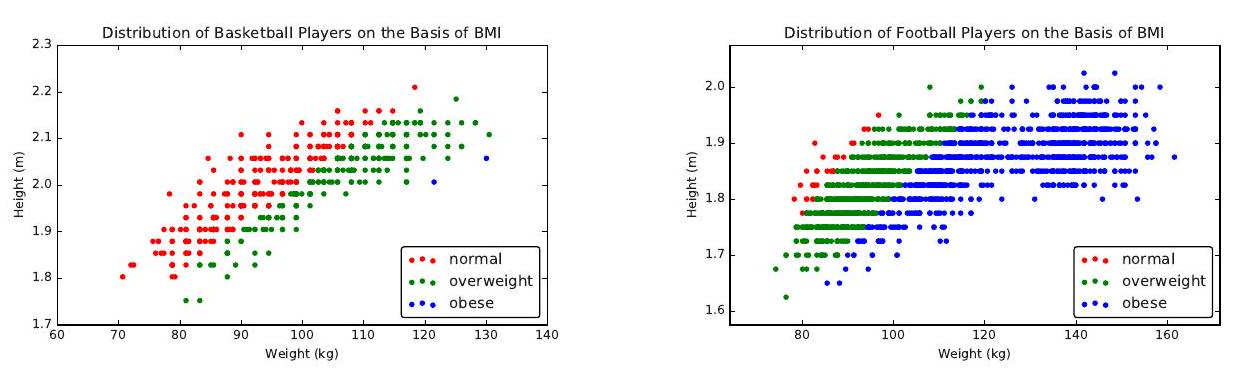
\includegraphics[max width=\textwidth]{2025_03_17_ca60ec0bfd96dcf8e028g-114(2)}
\caption{BMI \textenglish{distributions} \textenglish{of} \textenglish{professional} \textenglish{basketball} (\textenglish{left}) \textenglish{and} \textenglish{football} (\textenglish{right}) players.}
\end{figure}

\begin{figure}[htbp]
\centering
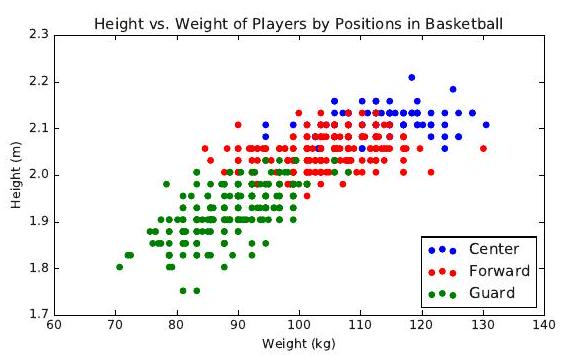
\includegraphics[max width=\textwidth]{2025_03_17_ca60ec0bfd96dcf8e028g-114(1)}
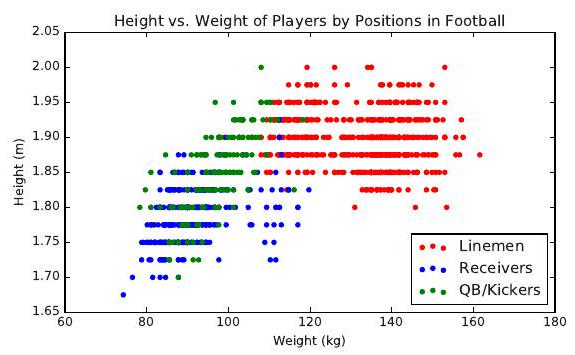
\includegraphics[max width=\textwidth]{2025_03_17_ca60ec0bfd96dcf8e028g-114}
\caption{Position \textenglish{in} \textenglish{basketball} (\textenglish{left}) \textenglish{and} \textenglish{football} (\textenglish{right}) \textenglish{is} \textenglish{largely} \textenglish{determined} \textenglish{by} size.}
\end{figure}

उनका बीएमआई सामान्य होता है हालांकि उनकी ऊँचाई बहुत असामान्य होती है। और फुटबॉल खिलाड़ी लगभग समान रूप से जानवर की तरह होते हैं, ज़्यादातर मोटापे के रूप में स्कोर किए जाते हैं, भले ही वे अच्छी तरह से प्रशिक्षित एथलीट भी होते हैं। ये फुटबॉल खिलाड़ी आमतौर पर ताकत के लिए अनुकूलित होते हैं, न कि कार्डियोवेस्कुलर फिटनेस के लिए।

अध्याय~\ref{अध्याय:विज़ुअलाइज़ेशन}में, हम डेटा की प्रस्तुति को उजागर करने के लिए विज़ुअलाइज़ेशन तकनीकों पर चर्चा करेंगे, लेकिन चलो यहां से अपनी सौंदर्य दृष्टि को विकसित करना शुरू करते हैं। हम\textit{स्कैटर प्लॉट्स}का उपयोग करते हैं ताकि प्रत्येक व्यक्ति को ऊंचाई-वजन स्थान में एक बिंदु के रूप में दिखाया जा सके, जिसमें लेबल (वजन वर्ग या खिलाड़ी स्थिति) रंगों के रूप में दिखाए जाते हैं।

बीएमआई का पद के अनुसार वितरण भी खुलासा करता है, जैसा कि चित्र~4.3 में दिखाया गया है। बास्केटबॉल में, गार्ड्स तेज़ और पतले होते हैं जबकि सेंटर्स लंबे और डराने वाले होते हैं। इसलिए ये सभी पद अलग-अलग आकार के अनुसार व्यवस्थित हैं। फुटबॉल में, स्किल खिलाड़ियों (क्वार्टरबैक, किकर्स, और पंटर्स) की बनावट लाइन पर खड़े भारी खिलाड़ियों की तुलना में काफी छोटी होती है।

\section{स्कोरिंग सिस्टम विकसित करना}
\index{developing \textenglish{scoring} systems}स्कोर्स ऐसी क्रियाएँ हैं जो प्रत्येक इकाई की विशेषताओं को योग्यता के एक संख्यात्मक मूल्य में परिवर्तित करती हैं। यह अनुभाग प्रभावी स्कोरिंग सिस्टम बनाने और उनका मूल्यांकन करने के मूल दृष्टिकोणों पर नजर डालेगा।\index{data-driven!models}\index{modeling!data-driven}\index{modeling!first-principle}

\subsection{स्वर्ण मानक और प्रॉक्सी}
\index{proxies}\index{gold standards}इतिहासically, \textenglish{paper} \textenglish{currencies} सोना द्वारा समर्थित थे, जिसका मतलब था कि एक \textenglish{paper} \textenglish{dollar} को हमेशा\$1 मूल्य का सोना बदला जा सकता था। यही कारण था कि हम जानते थे कि हमारा पैसा उस \textenglish{paper} से अधिक मूल्यवान था जिस पर इसे छापा गया था।

डेटा विज्ञान में, a\textit{सुनहरा मानक} उन लेबल्स या उत्तरों का समूह होता है जिन पर हमें सही होने का भरोसा होता है। मूल बीएमआई के सूत्रीकरण में, सुनहरा मानक शरीर की चर्बी के प्रतिशत थे जो थोड़ी संख्या में विषयों पर सावधानीपूर्वक मापे गए थे। स्वाभाविक रूप से, ऐसे माप कुछ त्रुटि के पात्र होते हैं, लेकिन जब हम इन मूल्यों को फिटनेस के लिए सुनहरा मानक परिभाषित करते हैं, तो हम उन्हें सही माप के रूप में स्वीकार करते हैं। सोने में हम विश्वास करते हैं।

सोने के मानक की उपस्थिति एक अच्छे स्कोरिंग प्रणाली विकसित करने के लिए एक कठोर तरीका प्रदान करती है। हम \ref{linear regression} जैसी कर्व-फिटिंग तकनीकों का उपयोग कर सकते हैं (जिस पर ⸨Section~sec:linear_regression⸩ में चर्चा की जाएगी) ताकि इनपुट विशेषताओं का वजन इस तरह से दिया जा सके कि वे सोने के मानक उदाहरणों पर "सही उत्तरों" के सर्वोत्तम सन्निकटन कर सकें।

लेकिन असली सोने के मानक ढूँढना कठिन हो सकता है। \textit{प्रतिनिधि} उन आंकड़ों को खोजना आसान होता है, जो वांछित लेकिन अप्राप्य वास्तविकता के साथ अच्छे से सहसंबंधित होना चाहिए। बीएमआई का डिज़ाइन शरीर की वसा प्रतिशत के लिए एक प्रतिनिधि के रूप में किया गया था। इसे केवल ऊँचाई और वजन से आसानी से गणनीय किया जा सकता है, और यह शरीर की वसा के साथ अच्छा सहसंबंध स्थापित करता है। इसका मतलब है कि शायद ही कभी पानी के टैंक में तैरने की क्षमता की जाँच करने की या कैलिपर्स से “इंच पिंचने” की आवश्यकता होती है, जो अधिक दखल देने वाले उपाय हैं जो सीधे किसी व्यक्ति की मोटापे को मापने की मात्रा निर्धारित करते हैं।

मान लीजिए मैं अगले वर्ष के डेटा विज्ञान पाठ्यक्रम के लिए उपयोग किए जाने वाले ग्रेडिंग सिस्टम में सुधार करना चाहता हूँ। मेरे पास पिछले वर्ष के छात्र डेटा हैं, इसका मतलब है उनके होमवर्क और टेस्ट के स्कोर, लेकिन मेरे पास ऐसा कोई स्वर्ण मानक नहीं है जिससे मैं यह समझ सकूँ कि इन छात्रों को कौन से ग्रेड \textit{प्राप्त} होने चाहिए। मेरे पास केवल वही ग्रेड हैं जो मैंने उन्हें दिए थे, जो प्रणाली में सुधार करने की कोशिश करते समय अर्थहीन हैं।

मुझे उनके अज्ञात "वास्तविक" पाठ्यक्रम योग्यता का एक प्रॉक्सी चाहिए। इसके लिए एक अच्छा उम्मीदवार प्रत्येक छात्र का उनके \textit{अन्य} पाठ्यक्रमों में कुल \textenglish{GPA} हो सकता है। सामान्य रूप से, छात्र प्रदर्शन को पाठ्यक्रमों के बीच संरक्षित रहना चाहिए। यदि मेरी मूल्यांकन प्रणाली सबसे अच्छे छात्रों के \textenglish{GPA} को नुकसान पहुंचाती है और निचले स्तर के छात्रों की मदद करती है, तो संभवतः मैं कुछ गलत कर रहा हूँ।

प्रॉक्सी स्कोरिंग/रैंकिंग प्रणालियों का मूल्यांकन करते समय विशेष रूप से अच्छे होते हैं। हमारी किताब\textit{कौन बड़ा है?}~\cite{SW13} में हमने "महत्व" के आधार पर ऐतिहासिक व्यक्तियों को रैंक करने के लिए विकिपीडिया का उपयोग किया। हमारे पास यह मापने के लिए कोई गोल्ड मानक महत्व डेटा नहीं था कि ये लोग\textit{वास्तव में}कितने महत्वपूर्ण थे। लेकिन हमने कई प्रॉक्सी का उपयोग किया यह मूल्यांकन करने के लिए कि हम कितने सही थे, ताकि हमें ईमानदार बने रहें:

\begin{itemize}
  \item मशहूर हस्तियों से मिलने वाले ऑटोग्राफ के लिए संग्राहकों द्वारा चुकाई जाने वाली कीमतें \textit{आम तौर पर} मशहूर हस्ती के महत्व के साथ सहसंबंधित होनी चाहिए। जितनी अधिक कीमत लोग चुकाने को तैयार होंगे, उतना बड़ा सितारा होगा।
  \item बेसबॉल खिलाड़ी की कितनी अच्छी स्थिति है, इसके आँकड़े \textit{आम तौर पर} खिलाड़ी की महत्वपूर्णता के साथ सहसंबंधित होने चाहिए। जितना बेहतर खिलाड़ी, उतना अधिक महत्वपूर्ण होने की संभावना।\index{deep learning!models}\index{discounting}\index{modeling!deep learning}\index{modeling!flat}\index{modeling!hierarchical}
  \item पुस्तकों और पत्रिकाओं में प्रकाशित रैंकिंग शीर्ष राष्ट्रपतियों, फिल्म सितारों, गायकों, लेखकों, आदि की सूची बनाती हैं। इतिहासकारों द्वारा उच्च रैंक वाले राष्ट्रपति आम तौर पर हमारे द्वारा भी उच्च रैंक वाले होने चाहिए। इस प्रकार की राय, समग्र रूप से, आम तौर पर इन ऐतिहासिक व्यक्तियों के महत्व के साथ सहसंबंधित होनी चाहिए।
\end{itemize}

हम धारा \ref{sec:historical_significance} में हमारे ऐतिहासिक महत्व स्कोरों के कार्यप्रणाली के बारे में अधिक विस्तृत रूप से चर्चा करेंगे।

\subsection{स्कोर्स बनाम रैंकिंग}
\textit{रैंकिंग} मेरिट के अनुसार \textenglish{n} संस्थाओं को क्रमबद्ध करने के लिए क्रमचय होते हैं, जो आमतौर पर किसी स्कोरिंग प्रणाली के आउटपुट को क्रमबद्ध करके बनाए जाते हैं। रैंकिंग/रेटिंग प्रणालियों के लोकप्रिय उदाहरणों में शामिल हैं:



%---- \textenglish{Page} \textenglish{End} \textenglish{Break} \textenglish{Here} ---- \textenglish{Page} : 100







$A = 4.0)$। लेकिन प्राकृतिक रूप से भिन्नताओं की संभावना होती है: कई स्कूल सम्मान पाठ्यक्रमों को अधिक वजन देते हैं बजाय जिम जैसे हल्के क्लासेज के, ताकि अच्छे ग्रेड प्राप्त करने की कठिनाई को दर्शा सके।

आम तौर पर, किसी स्कोरिंग सिस्टम के परिणामों को सॉर्ट करने से एक संख्यात्मक रैंकिंग प्राप्त होती है। लेकिन दूसरी तरह से सोचें, तो प्रत्येक वस्तु की रैंकिंग स्थिति (जैसे, 2196 में से 493वां) उस वस्तु के लिए एक संख्यात्मक स्कोर भी प्रदान करती है।

चूंकि स्कोर और रैंकिंग एक दूसरे के द्वैत होते हैं, कौन सा डेटा का अधिक अर्थपूर्ण प्रस्तुतिकरण प्रदान करता है? किसी भी तुलना की तरह, सबसे अच्छा उत्तर यह है कि यह निर्भर करता है, जैसे मुद्दों पर:

\begin{itemize}
  \item \textit{क्या संख्याएँ अलग-थलग रूप में प्रस्तुत की जाएँगी?} रैंकिंग स्कोर के विवेचन के लिए संदर्भ देने में अच्छी होती हैं। जब मैं यह लिख रहा हूँ, स्टोनी ब्रुक की बास्केटबॉल टीम देश की 351 कॉलेज टीमों में 111वें स्थान पर है, हमारे \textenglish{RPI} (रेटिंग्स प्रतिशत इंडेक्स) 39.18 के बल पर। कौन सा नंबर आपको यह बेहतर समझाने में मदद करता है कि हमारी टीम अच्छी है या खराब, 111वां या 39.18?
  \item \textit{स्कोर का अंतर्निहित वितरण क्या है?} परिभाषा के अनुसार, शीर्ष रैंक वाली इकाई का स्कोर दूसरे स्थान की तुलना में बेहतर होता है, लेकिन यह आपको उनके बीच के अंतर के परिमाण के बारे में कुछ नहीं बताता। क्या वे लगभग बराबरी पर हैं, या \#1 उन्हें पछाड़ रहा है?
\end{itemize}

\index{Occam’s razor}
रैंकिंग में अंतर \textit{दिखाई} देने में रैखिक प्रतीत होते हैं: 1 और 2 के बीच का अंतर 111 और 112 के बीच के अंतर के समान लगता है। लेकिन यह सामान्य रूप से स्कोरिंग प्रणाली में सही नहीं है। वास्तव में, छोटे पूर्ण स्कोरिंग अंतर अक्सर बड़े रैंकिंग अंतर ला सकते हैं।\index{classification!evaluating}\index{negative class}\index{positive class}

\begin{itemize}
  \item \textit{क्या आप चरम सीमाओं या मध्य के बारे में परवाह करते हैं?} अच्छी तरह से डिज़ाइन की गई स्कोरिंग प्रणालियों में अक्सर एक घंटे के आकार का वितरण होता है। औसत के आसपास केंद्रित अंकों के साथ, अंकों में छोटे अंतर रैंक में बड़े बदलाव ला सकते हैं। एक सामान्य वितरण में, अपने स्कोर को मानक विचलन ($\sigma$) से बढ़ाना आपको 50वें प्रतिशत से 84वें प्रतिशत तक ले जाता है। लेकिन $1\sigma$ से $2\sigma$ तक उसी आकार का परिवर्तन आपको केवल 84वें से 92.5वें प्रतिशत तक ले जाता है।
\end{itemize}

तो जब एक संगठन पहले से दसवें स्थान पर फिसलता है, तो कार्रवाई करनी चाहिए। लेकिन जब स्टोनी ब्रूक की टीम 111वें से 120वें स्थान पर फिसलती है, तो यह शायद अंक में एक महत्वहीन अंतर को दर्शाता है और इसे नजरअंदाज किया जाना चाहिए। रैंकिंग समूह के अत्यधिक उत्कृष्ट और अत्यधिक खराब संस्थाओं को उजागर करने में तो अच्छी हैं, लेकिन औसत के निकट के अंतरों को उतना नहीं।

\subsection{अच्छे स्कोरिंग फंक्शंस की पहचान}

अच्छे स्कोरिंग फंक्शन्स अच्छे होते हैं क्योंकि वे आसानी से समझे जा सकते हैं और सामान्यतः विश्वसनीय होते हैं। यहाँ हम उन गुणों की समीक्षा कर रहे हैं जो आकड़े विज्ञान में इन दिशाओं की ओर संकेत करते हैं:

\begin{itemize}
  \item \textit{आसानी से गणना योग्य:} अच्छे आँकड़ों को आसानी से वर्णित और प्रस्तुत किया जा सकता है। बीएमआई एक उत्कृष्ट उदाहरण है: इसमें केवल दो पैरामीटर होते हैं, और इसे केवल सरल बीजगणित का उपयोग करके मूल्यांकन किया जाता है। इसे कुछ आसानी से प्राप्त होने वाले, प्रासंगिक वेरिएबल्स पर सभी सरल क्रियात्मक रूपों के माध्यम से खोज के परिणामस्वरूप पाया गया था। यह अभ्यास के लिए आपके द्वारा अच्छी तरह से ज्ञात डेटा सेट पर किसी दिए गए फीचर सेट से संभावित आँकड़ों के विचार उत्पन्न करने का एक उत्कृष्ट व्यायाम है।
  \item \textit{आसानी से समझ में आने वाले:} आँकड़ों के वर्णन से स्पष्ट होना चाहिए कि रैंकिंग प्रश्न से संबंधित है। "ऊंचाई के अनुसार समायोजित भार" बताता है कि बीएमआई क्यों मोटापे के साथ जुड़ा हुआ है। आपके आँकड़े के पीछे के विचारों को स्पष्ट रूप से समझाना अन्य लोगों के लिए इसे उपयोग करने के लिए पर्याप्त विश्वास करने के लिए आवश्यक है।
  \item \textit{वेरिएबल्स की मोनोटोनिक व्याख्याएँ:} \index{coordination!interpretation}आपको यह समझ होनी चाहिए कि आपके स्कोरिंग फ़ंक्शन में उपयोग किए जाने वाले प्रत्येक फीचर का उद्देश्य से कैसे संबंध है। बीएमआई के साथ वजन\textit{को} सकारात्मक रूप से संबंध होना चाहिए, क्योंकि भारी होना बहुत वजन के होने की मांग करता है। ऊंचाई \textit{को} नकारात्मक रूप से संबंध होना चाहिए, क्योंकि लंबे लोग स्वाभाविक रूप से छोटे लोगों से अधिक वजन करते हैं।\index{accuracy}\index{monkey}\index{precision}\index{sharp}
  
  सामान्य तौर पर, आप एक वास्तविक स्वर्ण मानक के बिना एक स्कोरिंग फ़ंक्शन का उत्पादन कर रहे हैं जिससे तुलना की जा सके। यह समझने की आवश्यकता है कि आपके वेरिएबल्स का क्या मतलब है, ताकि आपका स्कोरिंग फ़ंक्शन इस अस्पष्ट उद्देश्य के साथ सही से संबंधित हो सके।
  \item \textit{असमान्यों पर सामान्यतः संतोषजनक परिणाम उत्पन्न करता है:} आदर्श रूप से, आपको कुछ व्यक्तिगत बिंदुओं के बारे में इतना पता होता है कि आपको किसी भी उचित स्कोरिंग प्रणाली में उनका स्थान ज्ञात हो सके। अगर मुझे स्कोरिंग प्रणाली द्वारा प्रकट की गई शीर्ष इकाइयों की पहचान से वास्तव में आश्चर्य होता है, तो यह शायद एक बग है, कोई विशेषता नहीं। जब मैं अपने पाठ्यक्रमों में छात्रों के ग्रेड गणना करता हूं, तो मुझे उनकी कक्षा में किए गए प्रश्नों से कुछ सितारों और कुछ औसत छात्रों के नाम पहले से ही पता होते हैं। अगर मेरे द्वारा गणना किए गए ग्रेड इस दृष्टिकोणों से मेल नहीं खाते हैं, तो एक संभावित बग है जिसे ट्रैक करने की आवश्यकता है।
  
  अगर आंकड़ा वस्तुएं वास्तव में पूरी तरह अज्ञात हों, तो आपको अपने डोमेन को बेहतर तरीके से जानने में कुछ समय बिताना चाहिए। कम से कम, कृत्रिम उदाहरण ("सुपरस्टार" और "सुपरडॉर्क") का निर्माण करें जिनके फीचर मान इस प्रकार हों कि वे रैंकिंग के शीर्ष और निचले हिस्से के करीब हों, और फिर देखें कि वे वास्तविक आंकड़ों के साथ कैसे फिट होते हैं।
  \item \textit{व्यवस्थित रूप से सामान्यीकृत वेरिएबल्स का उपयोग करता है:} बेल के आकार के वितरनों से खींचे गए वेरिएबल्स स्कोरिंग फ़ंक्शन्स में समझदारी से व्यवहार करते हैं। अंत के किसी भी छोर पर प्रत्यक्षतः अच्छे/बुरे आइटम्स से संबंद्ध असमान्य होंगे, साथ ही मध्य में उन आइटम्स की एक चोटी होगी जिनके स्कोर सभी आपस में तुलनात्मक रूप से समान होने चाहिए।
  
  इन सामान्यतः-वितरित वेरिएबल्स को Z-स्कोर (अनुभाग 4.3 देखें) में बदल दिया जाना चाहिए इससे पहले कि उन्हें एक साथ जोड़ा जाए, ताकि सभी फीचर्स के तुलनात्मक माध्य और प्रसरण हों। इसके परिणामस्वरूप स्कोरिंग फ़ंक्शन के जादुई स्थिरांकों पर निर्भरता कम होती है ताकि भार की समायोजित की जा सके और कोई एकल फीचर परिणामों पर बहुत अधिक प्रभाव न डाले।
\end{itemize}

%---- \textenglish{Page} \textenglish{End} \textenglish{Break} \textenglish{Here} ---- \textenglish{Page} : 102

\begin{itemize}
    \item अर्थपूर्ण तरीकों से संबंध विच्छेद करता है: रैंकिंग फंक्शन का मूल्य तब बहुत सीमित हो जाता है जब वहां संबंध बनते हैं। लोगों की सुविधा का रैंकिंग कितनी उंगलियाँ उनके पास हैं, से करना बहुत खुलासा नहीं करेगा। बारह उंगलियों वाली एक बहुत ही चुनी हुई समूह होगी, दस के साथ बहुमत होगा, और फिर छोटे समूह जो दुर्घटना के शिकार होकर विकलांग हो गए हैं, जब तक हम शून्य तक नहीं पहुंच जाते।\\
    सामान्यतः, स्कोर को एक स्वस्थ सीमा में वास्तविक संख्याएं होना चाहिए, संबंधों की संभावना को न्यूनतम करने के लिए। संबंध विच्छेद करने के लिए माध्यमिक विशेषताओं को पेश करना मूल्यवान है, और समझ में आता है यदि ये विशेषताएं उस गुणधर्म के साथ भी संबंधित हैं जिसकी आपको परवाह है।
\end{itemize}

\section{Z-स्कोर और सामान्यीकरण}
डेटा विज्ञान का एक महत्वपूर्ण सिद्धांत यह है कि हमें अपने मॉडलों के लिए सही काम करना जितना संभव हो उतना आसान बनाना चाहिए। मशीन लर्निंग तकनीकें जैसे लीनियर रिग्रेशन यह दावा करती हैं कि वे दिए गए डेटा सेट के लिए एक उपयुक्त रेखा खोजती हैं। लेकिन कुछ फिट करने के लिए उनका उपयोग करने से पहले सभी विभिन्न वेरिएबल्स को सामान्यीकृत करना महत्वपूर्ण है ताकि उनकी रेंज/वितरण की तुलना की जा सके।\index{classification!balanced}

\textit{Z}-स्कोर्स सामान्यीकरण के हमारे प्राथमिक तरीका होगा।\textit{Z}-स्कोर रूपांतरण को इस प्रकार गणना की जाती है:

\begin{equation}
Z_{i}=\frac{(a_{i}-\mu)}{\sigma}
\end{equation}

जहाँ$\mu$वितरण का औसत है और$\sigma$संबंधित मानक विचलन है।\\
\textit{Z}-स्कोर्स चर समूहों को एक समान रेंज में परिवर्तित करते हैं। इंच में मापी गई ऊँचाई की \textit{Z}-स्कोर्स मील्स में मापी गई ऊँचाई के समान ही होंगी। सभी बिंदुओं पर एक \textit{Z}-स्कोर का औसत मान शून्य होता है। चित्र 4.4 एक पूर्णांकों के सेट को \textit{Z}-स्कोर्स में कम करके दिखाता है। औसत से बड़े मूल्य सकारात्मक हो जाते हैं, जबकि औसत से छोटे मूल्य नकारात्मक हो जाते हैं। \textit{Z}-स्कोर्स का मानक विचलन 1 है, इसलिए सभी \textit{Z}-स्कोर्स की वितरण समान विशेषताएँ होती हैं।

मानदंडों को\textit{Z}-स्कोर्स में बदलना दो उद्देश्यों को पूरा करता है। सबसे पहले, वे पैटर्न और सहसंबंधों को समझने में मदद करते हैं, यह सुनिश्चित करके कि सभी क्षेत्रों का समान माध्य (शून्य) हो और वे समान श्रेणी में काम करते हों। हम समझते हैं कि 3.87 का\textit{Z}-स्कोर बास्केटबॉल खिलाड़ी स्तर की ऊंचाई को इस प्रकार दर्शाता है, जैसा कि 79.8 नहीं करता, भले ही माप की इकाई (जैसे इंच) की जानकारी न हो। दूसरा,\textit{Z}-स्कोर्स का उपयोग हमारे मशीन लर्निंग ऐल्गोरिदमों को सहज बनाता है, क्योंकि यह सारी भिन्न विशेषताओं को एक तुलनीय पैमाने पर लाता है।

सिद्धांत रूप में, एक रेखीय परिवर्तन करने जैसे कि \textit{Z}-स्कोर वास्तव में कुछ भी नहीं करता जो अधिकांश शिक्षण एल्गोरिदम स्वयं ही पता नहीं कर सकते। ये एल्गोरिदम आमतौर पर सबसे अच्छा गुणांक निकालते हैं जिससे प्रत्येक चर को गुणा किया जा सके, जो स्वतंत्र है कि वह कितना भी छोटा$\sigma$लेने को यदि एल्गोरिदम वास्तव में उसे ऐसा ही करना चाहता है।

हालाँकि, संख्यात्मक गणना की वास्तविकताएँ यहाँ लागू होती हैं। मान लीजिए कि हम अमेरिका के शहरों से संबंधित दो चर की सहायता से एक रैखिक मॉडल बनाने का प्रयास कर रहे थे, जैसे, क्षेत्रफल में वर्ग मील और जनसंख्या। पहले का औसत लगभग 5 है और अधिकतम लगभग 100। दूसरे का औसत लगभग 25,000 है और अधिकतम 8,000,000। हमारे मॉडल पर दोनों चर का समान प्रभाव होने के लिए, हमें दूसरे चर को 100,000 या इसके लगभग के कारक से विभाजित करना होगा।

यह संख्यात्मक परिशुद्धता समस्याएँ उत्पन्न करता है, क्योंकि गुणांक के मान में बहुत छोटा परिवर्तन मॉडल में जनसंख्या चरों के प्रभुत्व के तरीके में बहुत बड़ा परिवर्तन करता है। बहुत बेहतर होगा कि चरों का मापदंड और वितरण सीमा मोटे तौर पर समान हो, ताकि मुद्दा यह हो कि एक विशेषता को, मान लें, किसी अन्य की तुलना में दोगुना शक्तिशाली कैसे वज़न दिया जाता है।

\textit{Z}-स्कोर्स का उपयोग सामान्यतः वितरित चरों में सबसे अच्छा होता है, जो अंततः माध्य$\mu$और मानक विचलन$\sigma$ द्वारा पूरी तरह वर्णित होते हैं। लेकिन वे उतने अच्छे से काम नहीं करते जब वितरण एक पावर लॉ हो। अमेरिका में धन वितरण पर विचार करें, जिसका एक माध्य (मान लें)\$200,000 हो सकता है, जिसमें a$\sigma=\$200,000$. \$80 बिलियन डॉलर के बिल गेट्स का\textit{Z}-स्कोर तब 4999 होगा, जो कि शून्य के माध्य के दिए जाने वाले में अभी भी एक उल्लेखनीय अपवाद है।\index{area \textenglish{under} \textenglish{the} \textenglish{ROC} curve}\index{Google News}\index{Mosteller, Frederick!evaluating}\index{top-k \textenglish{success} rate}

आपकी सबसे बड़ी डेटा विश्लेषण की गलतियाँ तब होंगी जब आप अपने विश्लेषण में ग़लत तरीक़े से सामान्यीकृत वेरियबल्स का उपयोग करेंगे। हम बिल गेट्स को कैसे निचे ला सकते हैं? हम उन्हें एक ⸨लॉग⸩ से मार सकते हैं, जैसा कि हमने ⸨सेक्शन⸩ 2.4 में चर्चा की थी।

\section{उन्नत रैंकिंग तकनीकें}
\index{rankings!techniques}अधिकांश बुनियादी रैंकिंग कार्य फीचर्स के रैखिक संयोजनों के रूप में स्कोर की गणना करके और फिर उन्हें क्रमबद्ध करके हल किए जाते हैं। किसी भी स्वर्ण मानक की अनुपस्थिति में, ये विधियाँ आँकड़े उत्पन्न करती हैं जो अक्सर रहस्योद्घाटन करने वाले और जानकारीपूर्ण होते हैं।

हालाँकि, कई शक्तिशाली तकनीकें विकसित की गई हैं जो विशिष्ट प्रकार की इनपुट्स से रैंकिंग्स की गणना करती हैं: ⸨पेयर की तुलना⸩ के परिणाम, ⸨संबंध नेटवर्क⸩, और यहाँ तक कि ⸨अन्य रैंकिंग्स के समूह⸩ भी। हम यहाँ इन विधियों की समीक्षा करते हैं, प्रेरणा के लिए।

\subsection{एलो रैंकिंग्स}
\index{Elo rankings}रैंकिंग्स अक्सर बाइनरी तुलना के अनुक्रमों का विश्लेषण करके बनाई जाती हैं, जो संस्थाओं के बीच प्रतियोगिताओं में स्वाभाविक रूप से उत्पन्न होती हैं।
%---- पृष्ठ समाप्ति विराम यहां ---- पृष्ठ : 104



\begin{itemize}
  \item \textit{खेल प्रतियोगिता परिणाम}: सामान्य खेल आयोजनों में, चाहे वे फुटबॉल मैच हों या शतरंज की प्रतियोगिताएं, टीम $A$ और $B$ एक-दूसरे के खिलाफ होती हैं। इनमें से केवल एक ही जीतेगा। इस प्रकार प्रत्येक मैच मूलतः योग्यता की बाइनरी तुलना है।
  \item \textit{वोट और पोल}: जानकार व्यक्तियों से अक्सर विकल्पों की तुलना करने और यह निर्णय लेने के लिए कहा जाता है कि कौन सा चयन बेहतर है। एक चुनाव में, इन तुलनाओं को वोट कहा जाता है। कुछ विश्वविद्यालय रैंकिंग का एक प्रमुख घटक प्रोफेसरों से यह पूछने पर आता है: कौन सा स्कूल बेहतर है, $A$ या $B$?
\end{itemize}

फ़िल्म \textit{द सोशल नेटवर्क} में, फेसबुक के मार्क ज़ुकरबर्ग को फेसमैश से शुरुआत करते हुए दिखाया गया है, एक वेबसाइट जो दर्शकों को दो चेहरे दिखाती है और उनसे पूछती है कि कौन सा अधिक आकर्षक है। उनकी साइट फिर इन जोड़ीदार तुलना के आधार पर सभी चेहरों को सबसे अधिक से सबसे कम आकर्षक तक रैंक करती थी।

\begin{itemize}
  \item \textit{अन्तर्निहित तुलना}: सही दृष्टिकोण से देखने पर, विशेष तिथियों को युग्मित तुलनाओं के रूप में अर्थपूर्ण रूप से व्याख्या किया जा सकता है। मान लीजिए कि एक छात्र को दोनों विश्वविद्यालयों $A$ और $B$ द्वारा स्वीकार कर लिया गया है, लेकिन उसने $A$ को चुना। इसे इस रूप में लिया जा सकता है कि $A$ $B$ से बेहतर है।
\end{itemize}

ऐसे वोटों के संग्रह की सही व्याख्या क्या है, विशेष रूप से जहाँ कई उम्मीदवार होते हैं, और सभी खिलाड़ियों की जोड़ी एक-दूसरे से सीधे मुकाबला नहीं करती है? यह कहना उचित नहीं है कि सबसे अधिक जीतने वाला ही विजेता होता है, क्योंकि (\textenglish{a}) उन्होंने अन्य खिलाड़ियों की तुलना में अधिक मुकाबलों में हिस्सा लिया हो सकता है, और (\textenglish{b}) उन्होंने मजबूत प्रतिद्वंद्वियों से बचकर केवल कमजोर प्रतिस्पर्धा को हराया हो सकता है।

\textit{एलो प्रणाली}सभी खिलाड़ियों को समान रूप से आंकी जाने वाली दर से शुरू होती है, और फिर प्रत्येक मैच के परिणाम के अनुसार प्रत्येक खिलाड़ी के स्कोर को धीरे-धीरे समायोजित करती है, सूत्र के अनुसार:\index{error}\index{error!absolute}\index{error!statistics}\index{precision}\index{recall}\index{value prediction!evaluating}

\[
r^{\prime}(\textenglish{A}) = r(\textenglish{A}) + k(S_{A} - \mu_{A})
\]

जहाँ

\begin{itemize}
  \item $r(\textenglish{A})$ और $r^{\prime}(\textenglish{A})$ खिलाड़ी $A$ के लिए पहले और अद्यतन स्कोर को दर्शाते हैं। 
  \item $k$ एक स्थिर पैरामीटर है जो एकल मैच के जवाब में अधिकतम संभावित स्कोर समायोजन को दर्शाता है। $k$ का छोटा मान काफी स्थिर रैंकिंग का परिणाम देता है, जबकि बहुत बड़ा $k$ नवीनतम मैच के आधार पर रैंकिंग में असमंजसकारी बदलाव लाएगा। 
  \item $S_{A}$ उस मैच में खिलाड़ी $A$ द्वारा प्राप्त स्कोर परिणाम है। सामान्यतः, $S_{A} = 1$ अगर $A$ जीतता है, और $S_{A} = -1$ अगर $A$ हार जाता है। 
  \item $\mu_{A}$ खिलाड़ी $A$ के लिए $B$ के खिलाफ प्रतियोगिता करते समय अपेक्षित परिणाम था। अगर $A$ और $B$ का कौशल स्तर ठीक एक जैसा है, तो संभवतः $\mu_{A} = 0$। लेकिन मान लीजिए कि $A$ एक चैंपियन है और $B$ एक शुरुआत करने वाला है। हमारी अपेक्षा है कि $A$ को एक हेड-टू-हेड मुकाबले में निश्चित रूप से जीतना चाहिए, क्योंकि $\mu_{A} > 0$ और यह 1 के काफी करीब हो सकता है। 
\end{itemize}



यहाँ सब कुछ साफ़ है सिवाय इसके कि$\mu_{A}$का निर्धारण कैसे किया जाए। यदि आपको यह संभावना दी गई है कि$A$, $B$को हराता है($P_{A>B}$), तब

\[
\mu_{A} = 1 \cdot P_{A>B} + (-1) \cdot (1 - P_{A>B})
\]

यह जीत की प्रायिकता स्पष्ट रूप से खिलाड़ियों के बीच कौशल अंतर की मात्रा पर निर्भर करती है$A$और$B$, जिसे रैंकिंग प्रणाली द्वारा मापा जाना चाहिए। इस प्रकार$x = r(\textenglish{A}) - r(\textenglish{B})$यह कौशल अंतर को दर्शाता है।

रैंकिंग प्रणाली को पूरा करने के लिए, हमें एक तरीका चाहिए जिससे इस वास्तविक चर$x$को एक अर्थपूर्ण संभावना में परिवर्तित किया जा सके। यह एक महत्वपूर्ण समस्या है जिसका हम इस पुस्तक में बार-बार सामना करेंगे, जिसे गणित के एक भाग\textit{लॉजिट फंक्शन}द्वारा हल किया जाता है।

\subsection{लॉजिट कार्य}
मान लें कि हम एक वास्तविक चर$-\infty< \textenglish{x} <\infty$को लें और इसे एक प्रायिकता$0\leqp\leq1$ में परिवर्तित करना चाहते हैं। यह करने के कई तरीके हो सकते हैं, लेकिन एक विशेष सरल परिवर्तन$p = f(\textenglish{x})$ है, जहाँ

\[
f(\textenglish{x}) = \frac{1}{1 + e^{-cx}}
\]

लॉजिट फंक्शन$f(\textenglish{x})$का आकार चित्र 4.5 में दिखाया गया है। विशेष रूप से मध्य और अंतिम बिंदुओं पर विशेष मामलों पर ध्यान दें:

\begin{itemize}
  \item जब दो खिलाड़ी समान क्षमता के होते हैं, $x = 0$, और $f(0) = 1 / 2$, यह दर्शाता है कि दोनों खिलाड़ियों के जीतने की संभावना समान है। 
  \item जब खिलाड़ी $A$ के पास बहुत बड़ी बढ़त होती है, $x \rightarrow \infty$, और $f(\infty) = 1$, यह परिभाषित करता है कि $A$ मैच जीतने के लिए निश्चित है। \index{error!mean squared}\index{error!root \textenglish{mean} squared}
\end{itemize}

\begin{figure}[h]
\centering
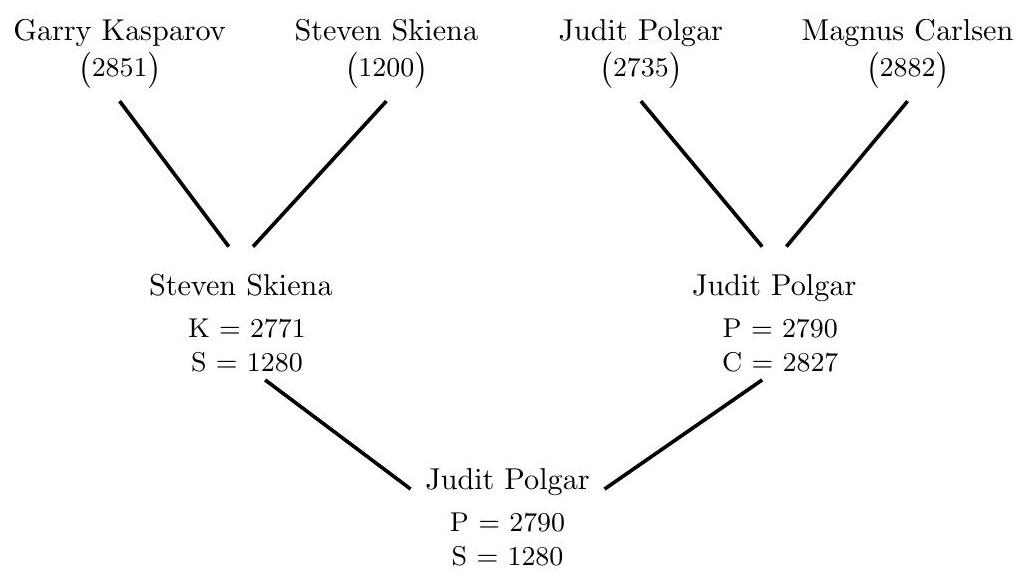
\includegraphics[max width=\textwidth]{2025_03_17_ca60ec0bfd96dcf8e028g-123}
\caption{Changes \textenglish{in} \textenglish{ELO} \textenglish{scores} \textenglish{as} \textenglish{a} \textenglish{consequence} \textenglish{of} \textenglish{an} \textenglish{unlikely} \textenglish{chess} tournament.}
\end{figure}

\begin{itemize} जब खिलाड़ी \itemB$ को बहुत बड़ा लाभ होता है, तो $x$ -\rightarrow\infty और $f(-$) = 0\infty, यह इंगित करता है कि $B$ निश्चित रूप से मैच जीतने वाला है। \end{itemize}

ये बिल्कुल वही मान हैं जिन्हें हम चाहते हैं अगर$x$खिलाड़ियों के बीच कौशल अंतर मापता है।

लॉजिट फंक्शन इन धाराओं के बीच कोमलता और समरूपता से अंतर प्रदान करता है। लॉजिट फंक्शन का पैरामीटर$c$ यह तय करता है कि संक्रमण कितना तीव्र होगा। क्या कौशल में छोटे अंतर जीतने की संभावना में बड़े अंतर में अनुवादित होते हैं? यदि$c = 0$है, तो परिदृश्य पैनकेक की तरह सपाट होता है:$f(\textenglish{x}) = 1 / 2$सभी$x$के लिए। जैसे-जैसे$c$ का मान बढ़ता है, संक्रमण तीव्र होता जाता है, जैसा कि चित्र 4.5 में दिखाया गया है। वास्तव में,$c =\infty बिल्कुल 0 से 1 तक का स्टेप फंक्शन होता है।

सेटिंग$c = 1$एक उचित शुरुआत है, लेकिन सही विकल्प डोमेन विशिष्ट होता है। यह देखना कि कितनी बार किसी दिए गए कौशल-अंतर की मात्रा आश्चर्यजनक रूप से परिणामित होती है (कमजोर पक्ष जीतता है) पैरामीटर को निर्दिष्ट करने में मदद करता है। \textenglish{Elo} चेस रैंकिंग प्रणाली इस प्रकार डिजाइन की गई थी कि$r(\textenglish{A}) - r(\textenglish{B}) = 400$का अर्थ है कि$A$के पास$B$की तुलना में जीतने की दस गुना संभावना है।

चित्र 4.6 \textenglish{Elo} गणनाओं को दर्शाता है, एक अत्यधिक असंभाव्य टूर्नामेंट के संदर्भ में जिसमें इतिहास के तीन महानतम शतरंज खिलाड़ी और एक निम्न श्रेणी के खिलाड़ी शामिल हैं। यहाँ पर $k = 40$ है, जो कि किसी एक मैच के परिणामस्वरूप अधिकतम संभव स्कोरिंग स्विंग 80 पॉइंट्स का संकेत देता है। मानक लॉजिट फंक्शन ने कास्पारोव को पहले राउंड में स्किएना को हराने की संभावना 0.999886 दी, लेकिन लाजर को जीवित करने जैसा चमत्कार होकर मैच विपरीत दिशा में चला गया। परिणामस्वरूप, 80 पॉइंट्स कास्पारोव की रैंकिंग से मेरी रैंकिंग में चले गए।

कोष्ठक के दूसरी तरफ दो वास्तविक शतरंज चैम्पियन्स ने मुकाबला किया, जिसमें पोल्गार द्वारा केवल 55 अंक की चाल चलकर अधिक कल्पनाशील उलटफेर किया गया। उन्होंने अंतिम राउंड में मुझसे साफ जीत हासिल की, जो एक ऐसा उपलब्धि थी जिसकी इतनी स्पष्ट अपेक्षा थी कि उन्होंने मूलतः शून्य रेटिंग अंक प्राप्त किए। इलो विधि सरप्राइज के प्रति रेटिंग को अपडेट करने में बहुत प्रभावी है, सिर्फ जीत नहीं।

%---- \textenglish{Page} \textenglish{End} \textenglish{Break} \textenglish{Here} ---- \textenglish{Page} : 107

\begin{center}
\begin{tabular}{l|cccll}
1 & \textenglish{A} & \textenglish{B} & \textenglish{A} & \textenglish{A} & $\mathrm{A}: 5$ \\
2 & \textenglish{C} & \textenglish{A} & \textenglish{B} & \textenglish{B} & $\mathrm{B}: 8$ \\\index{data!for evaluation}\index{data!for testing}\index{data!for training}\index{data formats!evaluation}
3 & \textenglish{B} & \textenglish{C} & \textenglish{C} & \textenglish{D} & $\mathrm{C}: 12$ \\
4 & \textenglish{D} & \textenglish{D} & \textenglish{E} & \textenglish{C} & $\mathrm{D}: 16$ \\
5 & \textenglish{E} & \textenglish{E} & \textenglish{D} & \textenglish{E} & $\mathrm{E}: 19$ \\
\end{tabular}
\end{center}

\textit{चित्र 4.7: बोर्डा की विधि का उपयोग करके चार इनपुट रैंकिंग के सेट से रैखिक भारों का उपयोग करते हुए $\{A, B, C, D, E\}$ की सहमति रैंकिंग का निर्माण।}

\subsection{रैंकिंग विलय करना}
कोई भी एकल संख्यात्मक विशेषता$f$, जैसे ऊँचाई, $\binom{n}{2} में से प्रत्येक जोड़े की तुलना करके$n$आइटम्स के बीच युग्मित तुलना की शुरुआत कर सकती है, यह परीक्षण करके कि क्या$f(\textenglish{A})>f(\textenglish{B})$प्रत्येक आइटम जोड़ी$A$और$B$के लिए। हम इन जोड़ों को$Elo विधि में फीड कर सकते हैं ताकि एक रैंकिंग प्राप्त की जा सके, लेकिन यह चीज़ों के बारे में सोचने का बेवकूफी भरा तरीका होगा। आखिरकार, किसी भी ऐसे विश्लेषण का परिणाम बस$f$ के क्रमित क्रम को ही प्रतिबिंबित करेगा।

कई अलग-अलग विशेषताओं द्वारा रैंकिंग के एक संग्रह को एकीकृत करना एक और दिलचस्प समस्या प्रस्तुत करता है। यहाँ हम$i$\,वाँ विशेषता के क्रमबद्ध क्रम को रुचि के आइटम पर एक परिमेय संपरिवर्त$P_{i}$के रूप में परिभाषित करते हैं। हम उस सर्वसम्मति संपरिवर्त$P$की खोज करते हैं, जो किसी तरह सभी घटक संपरिवर्तों$P_{1},\ldots, P_{k}$को सबसे अच्छी तरह प्रतिबिंबित करता है।

इसमें दो आकल्पनाओं के बीच समानता को मापने के लिए एक दूरी फलन को परिभाषित करना आवश्यक होता है। एक समान मुद्दा स्पीयरमैन रैंक सह-संबंध गुणांक को परिभाषित करते समय उत्पन्न हुआ (देखें अनुभाग 2.3.1), जहाँ हम तत्वों के सापेक्ष क्रम में सहमत माप से दो चरों की तुलना करते थे।\footnote{एक समानता माप और दूरी मेट्रिक के बीच अंतर को देखें। सह-संबंध में, स्कोर बड़े होते जाते हैं जैसे-जैसे तत्व अधिक समान होते जाते हैं, जबकि एक दूरी फलन में अंतर शून्य की ओर जाता है। दूरी मेट्रिक को अधिक विस्तार से अनुभाग 10.1.1 में चर्चा की जाएगी।}

\textit{बोर्डा की विधि}किसी सरलीकृत स्कोरिंग प्रणाली का उपयोग करके कई अन्य रैंकिंग्स से एक सर्वसम्मति रैंकिंग बनाती है। विशेष रूप से, हम क्रमपरिवर्तन की प्रत्येक$n$स्थितियों को एक लागत या वजन सौंपते हैं। फिर, प्रत्येक$n$तत्व के लिए, हम सभी$k$इनपुट रैंकिंग्स पर इसकी स्थिति के वज़नों का योग करते हैं। इन$n$स्कोरों को सॉर्ट करने से अंतिम सर्वसम्मति रैंकिंग निर्धारित होती है।

अब सभी कुछ स्पष्ट है सिवाय स्थितियों और लागतों के मानचित्रण के। सबसे सरल लागत फ़ंक्शन प्रत्येक क्रमपरिवर्तन में iवीं स्थिति में आने के लिए $i$ अंक सौंपता है, यानी हम सभी क्रमपरिवर्तन के ऊपर तत्व की रैंक को जोड़ते हैं। यही हम चित्र 4.7 के उदाहरण में करते हैं। वस्तु $A$ को तीन रैंकिंगों में पहले और एक में दूसरे आने की ताकत पर $3$1 + 1$2 = 5\cdot अंक मिलते हैं। वस्तु \cdotC$ $2, 3, 3$, और 4 पर समाप्त कर के 12 अंक प्राप्त करता है। अंतिम सर्वसम्मत रैंकिंग $\{A, B, C, D, E\}$ सभी इनपुट रैंकिंगों के सभी वोटों को एकीकृत करती है, भले ही सर्वसम्मति कम से कम भाग में सभी चार इनपुट रैंकिंग से असहमत हो।

लेकिन यह स्पष्ट नहीं है कि रैखिक वज़न का उपयोग करना सबसे अच्छा विकल्प है क्योंकि यह तत्वों की स्थिति में हमारी सटीकता पर समान विश्वास मानता है।



आमतौर पर, हम अपनी शीर्ष पसंदों की गुणों के बारे में सबसे अधिक जानते हैं, लेकिन उनके साधारण क्रम में आने वाली उन पसंदों के बारे में थोड़ा अस्पष्ट होते हैं। अगर ऐसा है, तो एक बेहतर दृष्टिकोण यह हो सकता है कि 1वें और 2वें के बीच के अंतर के लिए अधिक अंक दिए जाएं बनस्पत 110वें और 111वें के बीच के अंतर के।

इस प्रकार का वजन एक घंटी के आकार के वक्र द्वारा अप्रत्यक्ष रूप से किया जाता है। मान लीजिए कि हम एक सामान्य वितरण से समान अंतरालों पर$n$आइटमों का नमूना लेते हैं, जैसा कि चित्र 4.8 में दिखाया गया है। इन$x$मूल्यों को स्थानिक वजन के रूप में असाइन करने से केंद्र की तुलना में उच्चतम और सबसे निचले रैंकों पर अधिक फैलाव उत्पन्न होता है। टेल क्षेत्र वास्तव में उतने ही चौड़े होते हैं जितने वे इन 50 समान अंतराल बिंदुओं के लिए दिखते हैं: याद करें कि$95\%$संभाव्यता मास केंद्र के$2\sigmaके भीतर बैठती है।

वैकल्पिक रूप से, यदि हमारा विश्वास समान नहीं है, तो हम आधा-सामान्य वितरण से नमूना ले सकते हैं, ताकि हमारे रैंक्स की पूंछ सामान्य वितरण के शिखर द्वारा भारित हो जाए। इस प्रकार, उच्चतम रैंक वाले तत्वों के बीच सबसे अधिक विभाजन होता है, लेकिन पूंछ के तत्वों के बीच बहुत कम भेद होता है।

यहाँ आपका वजन फ़ंक्शन का चयन डोमेन-निर्भर है, इसलिए ऐसा चुनें जो आपकी समस्या पर अच्छा काम करता हो। सबसे\textit{अच्छा}कास्ट फ़ंक्शन की पहचान करना एक ग़लत ठहराया गया समस्या बन जाता है। और अजीब बातें होती हैं जब हम सही चुनाव प्रणाली डिजाइन करने की कोशिश करते हैं, जैसा कि सेक्शन 4.6 में दिखाया जाएगा।

\subsection{डाइग्राफ़-आधारित रैंकिंग}
\index{rankings!digraph-based}नेटवर्क एक वोट सेट के बारे में सोचने का वैकल्पिक तरीका प्रदान करते हैं जो " $A$को $B$से आगे रैंक करता है।" हम एक निर्दिष्ट ग्राफ़/नेटवर्क का निर्माण कर सकते हैं जहाँ प्रत्येक इकाई के लिए एक वरटेक्स हो, और प्रत्येक वोट के लिए एक निर्दिष्ट किनारा हो जो $A$को $B$से आगे रैंक करता है।

श्रेष्ठ क्रम इस प्रकार होगा कि शिखर$P$का एक पुनःविन्यास जो...

%---- \textenglish{Page} \textenglish{End} \textenglish{Break} \textenglish{Here} ---- \textenglish{Page} : 109

%---- \textenglish{Page} \textenglish{End} \textenglish{Break} \textenglish{Here} ---- \textenglish{Page} : 109

\begin{figure}[H]
\centering
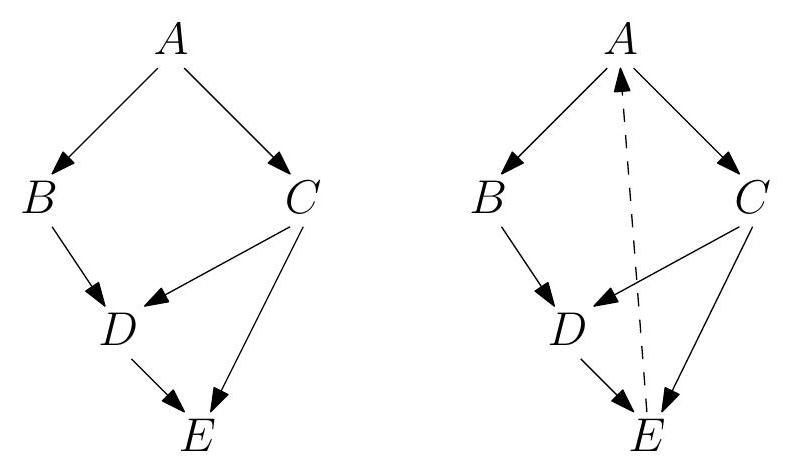
\includegraphics[max width=\textwidth]{2025_03_17_ca60ec0bfd96dcf8e028g-126}
\caption{Consistently \textenglish{ordered} \textenglish{preferences} \textenglish{yield} \textenglish{an} \textenglish{acyclic} \textenglish{graph} \textenglish{or} \textenglish{DAG} (\textenglish{left}). \textenglish{Inconsistent} \textenglish{preferences} \textenglish{result} \textenglish{in} \textenglish{directed} cycles, \textenglish{which} \textenglish{can} \textenglish{be} \textenglish{broken} \textenglish{by} \textenglish{deleting} \textenglish{small} \textenglish{sets} \textenglish{of} \textenglish{carefully} \textenglish{selected} edges, \textenglish{here} \textenglish{shown} \textenglish{dashed} (\textenglish{right}).}
\end{figure}

एक निर्देशित ग्राफ जिसमें चक्र नहीं होते हैं, उसे \textit{निर्देशित एसाइक्लिक ग्राफ} या \textit{डीएजी} कहा जाता है। कलन विधियों के थोड़े से पृष्ठभूमि ज्ञान वाले सतर्क पाठक को याद होगा कि इस आदर्श शीर्षक क्रम को ढूंढना \textit{विषयक रूप से छांटना}डीएजी को कहा जाता है, जिसे रैखिक समय में कुशलता से किया जा सकता है। चित्र 4.9 (बाएँ) एक डीएजी है, और इसमें निर्देशित किनारों के संगत दो विशिष्ट क्रम हैं: \textit{\{A, B, C, D, E\}} और \textit{\{A, C, B, D, E\}}।

लेकिन कुछ स्वाभाविक हीयूरिस्टिक्स हैं। एक अच्छा संकेत यह है कि एक वेर्टेक्स$v$कहाँ संबंधित है इसके इन-डिग्री और आउट-डिग्री के बीच का अंतर$d_{v}$ होता है। जब$d_{v}$बहुत नकारात्मक होता है, तो इसे शायद क्रम के सामने वाले हिस्से में होना चाहिए, क्योंकि यह कई तत्वों पर प्रभुत्व रखता है लेकिन केवल कुछ ही द्वारा प्रभुत्व में होता है। एक ठीक-ठाक रैंकिंग क्रम हमारे पास इन अंतरताओं के अनुसार वेर्टेसीज़ को सॉर्ट कर के बना सकते हैं। और भी बेहतर यह है कि सबसे नकारात्मक (या सबसे सकारात्मक) वेर्टेक्स$v$को उसके तार्किक स्थान पर क्रमिक रूप से डालें, $v$पर घटित हुई एजेस को हटाएँ, और फिर अगले सर्वश्रेष्ठ वेर्टेक्स को स्थिति देने से पहले गिनती को समायोजित करें।\index{Feynman, Richard}\index{modeling!simulation}\index{monotonic!simulations}

\section{पेजरैंक}
\index{PageRank}नेटवर्क में शीर्� \textbf{पेजरैंक}ल्गोरिदम शिक्षा से अधिक महत्वपूर्ण वर्णमाला का अध्याय बुक्क सर्च इंजन के शेरुखान लाइक का प्रदर्शन करता है।

वेब वेबपृष्ठों से बना है, जिनमें से अधिकांश में अन्य वेबपृष्ठों के लिंक होते हैं। आपका वेबपृष्ठ मेरे पृष्ठ से लिंक करता है, इसका तात्पर्य यह है कि आप समझते हैं कि मेरा पृष्ठ काफी अच्छा है। यदि इसे इस तरह के वोट के रूप में समझा जाए कि "आप समझते हैं कि मेरा पृष्ठ आपके से बेहतर है," तो हम लिंक का एक नेटवर्क बना सकते हैं और इसे अधिकतम अ-साइक्लिक-उपग्राफ समस्या के रूप में मान सकते हैं, जिसे पिछले उपविभाग में चर्चा की गई थी।

लेकिन प्रभुत्व वास्तव में वेब पर लिंक के लिए सही व्याख्या नहीं है। पेजरेंक इसके बजाय उन वर्टिसेज को पुरस्कृत करता है जिनके पास सबसे अधिक इन-लिंक होते हैं: यदि सभी रास्ते रोम की ओर जाते हैं, तो रोम एक काफी महत्वपूर्ण स्थान होना चाहिए। आगे, यह इन-लिंक्स को स्रोत की ताकत के आधार पर तौलता है: एक महत्वपूर्ण पेज से मुझे लिंक स्पैम साइट से एक की तुलना में अधिक महत्वपूर्ण होना चाहिए।

\section{युद्ध कहानी: क्लाइड की बदला}
\index{Clyde}हाई स्कूल के मेरे दूसरे वर्ष के दौरान, मुझे पेशेवर फुटबॉल खेलों के परिणाम का अनुमान लगाने के लिए एक प्रोग्राम लिखने का विचार आया। मुझे खेल के रूप में फुटबॉल में ज्यादा रुचि नहीं थी, लेकिन मैंने देखा कि मेरे कई सहपाठी सप्ताहांत के फुटबॉल खेलों के परिणाम पर अपनी लंच मनी पर दांव लगा रहे थे। मेरे लिए यह स्पष्ट था कि एक ऐसा प्रोग्राम लिखना जो फुटबॉल खेलों के परिणाम का सही अनुमान लगाए, उसका महत्वपूर्ण मूल्य हो सकता है, और इसके अलावा यह एक बहुत ही शानदार काम हो सकता है।

पुनरावलोकन में, वह प्रोग्राम जो मैंने तैयार किया था, अब निराशाजनक रूप से कच्चा लगता है। मेरा प्रोग्राम टीम$x$द्वारा बनाए गए अंकों का औसत और टीम$y$द्वारा दिए गए अंकों का औसत निकालता और भविष्यवाणी करता कि$x$कितने अंक$y$के खिलाफ बनाएगा।

\begin{equation}
\begin{aligned}
P_{x} &= \frac{((\text{points \textenglish{scored} \textenglish{by} \textenglish{team} } \textenglish{x}) + (\text{points \textenglish{allowed} \textenglish{by} \textenglish{team} } \textenglish{y}))}{2 \times (\text{games played})} \\
P_{y} &= \frac{((\text{points \textenglish{scored} \textenglish{by} \textenglish{team} } \textenglish{y}) + (\text{points \textenglish{allowed} \textenglish{by} \textenglish{team} } \textenglish{x}))}{2 \times (\text{games played})}
\end{aligned}
\end{equation}

यह कम्प्यूटर प्रोग्राम,\textit{क्लाइड}, वास्तविक दुनिया के किसी पक्ष के लिए एक स्कोरिंग फंक्शन बनाने का मेरा पहला प्रयास था। इसमें तर्क की एक निश्चित मात्रा मौजूद थी। अच्छी टीमें जितने अंक बनाती हैं उससे कम अंक छोड़ती हैं, जबकि खराब टीमें जितने अंक छोड़ती हैं उससे कम अंक बनाती हैं। यदि टीम$x$किसी टीम$y$के साथ खेलती है जिसने बहुत अधिक अंक छोड़े हैं, तो$x$को$y$के खिलाफ अधिक अंक बनाने चाहिए बजाय किसी अन्य टीम के खिलाफ जो मजबूत डिफेंस रखती है।

%---- \textenglish{Page} \textenglish{End} \textenglish{Break} \textenglish{Here} ---- \textenglish{Page} : 111

बेहतर रक्षा वाली टीमों के साथ। इसी तरह, जितने अधिक अंक टीम$x$ने बाकी लीग के खिलाफ हासिल किए हैं, उतने ज्यादा अंक वह$y$ के खिलाफ स्कोर करने की संभावना है।

बिल्कुल, यह साधारण मॉडेल फुटबॉल वास्तविकता के सभी पहलुओं को पकड़ नहीं सकता। मान लें कि टीम$x$अब तक सत्र में सिर्फ कमजोर टीमों के साथ खेल रही है, जबकि टीम$y$लीग की सर्वश्रेष्ठ टीमों के साथ खेल रही है। टीम$y$टीम$x$से कहीं बेहतर हो सकती है, भले ही अब तक का उसका रिकॉर्ड खराब हो। यह मॉडल टीम की किसी भी चोट को नजरअंदाज करता है, चाहे मौसम गर्म हो या ठंडा, और चाहे टीम गर्म हो या ठंडी। यह उन सभी कारकों को नजरअंदाज कर देता है जो खेलों को स्वाभाविक रूप से अप्रत्याशित बनाते हैं।

और फिर भी, इतना सरल मॉडल फुटबॉल खेलों के परिणाम की भविष्यवाणी करने में अच्छा काम कर सकता है। अगर आप ऊपर दिए गए तरीके से अंकों के औसत की गणना करते हैं, और घरेलू टीम को अतिरिक्त तीन अंक बोनस के रूप में देते हैं, तो आप लगभग दो-तिहाई फुटबॉल खेलों के विजेता को चुन लेंगे। इसकी तुलना सिक्का उछालने के और भी अनाड़ी मॉडल से करें, जो केवल आधे गेम सही ढंग से भविष्यवाणी करता है। यह पहला बड़ा सबक था जो क्लाइड ने मुझे सिखाया:

\textit{यहां तक कि कच्चे गणितीय मॉडल भी वास्तविक भविष्यवाणी शक्ति रख सकते हैं।}
\index{Mathematica}
एक साहसी 16 वर्षीय के रूप में, मैंने हमारे स्थानीय समाचार पत्र\textit{द न्यू ब्रंसविक होम न्यूज़}को लिखा, यह समझाते हुए कि मेरे पास फुटबॉल खेल के परिणामों की भविष्यवाणी करने के लिए एक कंप्यूटर प्रोग्राम है और मैं उन्हें मेरी भविष्यवाणियों को हर सप्ताह प्रकाशित करने का विशेष अवसर देने के लिए तैयार था। याद रखें कि यह 1977 की बात है, जब व्यक्तिगत कंप्यूटर जनता के ध्यान में नहीं आए थे। उन दिनों, एक हाई स्कूल के बच्चे का वास्तव में कंप्यूटर\textit{का उपयोग करना}काफी अद्भुत नवीनता मूल्य रखता था। यह समझने के लिए कि समय कितना बदल गया है, पेपर में क्लाइड और मेरे बारे में प्रकाशित लेख को फिगर 4.10 में देखें।

मुझे नौकरी मिल गई। क्लाइड ने 1977 नेशनल फुटबॉल लीग के प्रत्येक खेल के परिणाम की भविष्यवाणी की। जैसा कि मुझे याद है, क्लाइड और मैंने सीज़न को 135-70 के प्रतीत होने वाले प्रभावशाली रिकॉर्ड के साथ समाप्त किया। हर सप्ताह, वे मेरी भविष्यवाणियों की तुलना अखबार के खेल लेखक की भविष्यवाणियों से करते थे। जैसा कि मुझे याद है, हम सभी के रिकॉर्ड में कुछ ही खेलों का अंतर रहा, हालांकि अधिकांश खेल लेखक कंप्यूटर से बेहतर रिकॉर्ड के साथ समाप्त हुए।

\textit{होम न्यूज}मेरे काम से इतना प्रभावित था कि उन्होंने अगले सीजन के लिए मुझे नहीं रखा। हालांकि, 1978 सीजन के लिए क्लाइड की भविष्यवाणियाँ\textit{फिलाडेल्फिया इन्क्वायरर}में प्रकाशित हुईं, जो एक बहुत बड़ा अखबार था। हालांकि, मेरे पास कॉलम अकेले नहीं था। इसके बजाय,\textit{इन्क्वायरर}ने मुझे दस शौकिया और पेशेवर भविष्यवक्ताओं के साथ शामिल किया। हर हफ्ते हमें पॉइंट स्प्रेड के खिलाफ चार खेलों के परिणामों की भविष्यवाणी करनी थी।

फ़ुटबॉल में पॉइंट स्प्रेड बेटिंग उद्देश्यों के लिए मजबूत टीमों को हैंडीकैप करने का एक तरीका है। पॉइंट स्प्रेड को इस तरह से डिजाइन किया जाता है कि हर खेल को एक 50/50 प्रस्ताव बना देता है, और इसलिए खेलों के परिणाम का पूर्वानुमान लगाना बहुत कठिन होता है।

क्लाइड और मैंने 1978 के नेशनल फ़ुटबॉल लीग सीज़न के दौरान स्प्रेड के खिलाफ बहुत अच्छा प्रदर्शन नहीं किया, और ना ही अधिकतर अन्य \textit{फिलाडेल्फिया इन्क्वायरर} भविष्यवक्ताओं ने। हमने केवल 46\% खेलों की सही भविष्यवाणी की स्प्रेड के खिलाफ, जो कि दस प्रकाशित भविष्यवक्ताओं में से 7वें स्थान पर खत्म करने के लिए पर्याप्त (या खराब) प्रदर्शन था। स्प्रेड के खिलाफ भविष्यवाणी करने से मुझे दूसरा प्रमुख जीवन पाठ मिला:

\section{मृवंत कंप्यूटर का उपयोग फुटबॉल के विजेता की भविष्यवाणी करने के लिए करता है}
\index{football}ईस्ट ब्रंसविक - 16 वर्षीय ईस्ट ब्रंसविक हाई स्कूल का छात्र ने फुटबॉल में रुचि को कंप्यूटर के प्रति आकर्षण के साथ जोड़ने का एक तरीका खोजा है।

स्टीवन स्कियेना कहते हैं कि वे प्रतिस्पर्धा करने वाली टीमों के बारे में आवश्यक जानकारी कंप्यूटर को देकर पेशेवर फुटबॉल खेलों के परिणाम को उच्च सटीकता के साथ निर्धारित कर सकते हैं।

"विजेता लगभग हमेशा सही होंगे," ने कहा हाई स्कूल जूनियर ने, जो 5 कूरियर रोड पर रहता है, डन्हम्स कॉर्नर रोड से हटकर। "मेरा अनुमान लगाने में 85 प्रतिशत की सटीकता दर थी जब मैंने पिछले सीज़न के अंत में अनुमान लगाना शुरू किया था।"

वह इसे इस तरह करता है कि वह कंप्यूटर को टीम रिकॉर्ड, बनाए गए और दिए गए पॉइंट्स, खेल के दौरान प्राप्त और दिए गए औसत यार्ड्स, प्राप्त और दिए गए यार्ड्स को रशिंग और पासिंग श्रेणियों में विभाजित करना, घर पर और यात्रा पर प्रदर्शन और अन्य कई आँकड़े खिलाता है।

जानकारी को फुटबॉल सांख्यिकी और रैंकिंग के साप्ताहिक संकलनों से एकत्र किया जाता है। स्कीना तथ्यों को सूचकांक कार्ड पर लिखते हैं और फिर उन्हें हाई स्कूल के छह कंप्यूटर टर्मिनल में से एक या ⸨लाइब्रेरी⸩ के टर्मिनल पर टाइप करते हैं, जहाँ वे स्कूल के बाद अंशकालिक काम करते हैं।

"मुझे एक विजयी टीम, प्रत्येक टीम के लिए एक दशमलव स्कोर और एक अंकों का फैलाव मिलता है," कहा उस किशोर ने जिसने पिछले साल हाई स्कूल में कंप्यूटर प्रोग्रामिंग कोर्स पूरा किया।

उसका पहले प्रयास विजेताओं को चुनने का सोमवार की रात के खेल में शामिल था जो ओकलैंड रेडर्स, जो बाद में सुपर बॉल के विजेता बने, और सिंसिनाटी बेंगल्स के बीच था।

यह विश्लेषण के लिए एक कठिन खेल था क्योंकि सिनसिनाटी प्लेऑफ बर्थ के लिए लड़ाई कर रहा था जबकि ओकलैंड ने पहले ही पोस्ट-सीजन प्रतियोगिता में एक स्थान सुनिश्चित कर लिया था।

"कोई नहीं जानता था कि ओकलैंड 100 प्रतिशत देगा या नहीं," स्किएना ने कहा। "लेकिन मेरी गणनाओं ने संकेत दिया कि वे 24-20 से जीतेंगे। अंतिम स्कोर 35-20 था। उन्होंने पूरी कोशिश की।"

स्कीना ने कहा कि उन्होंने अगले हफ्ते 14 में से 12 विजेताओं को चुना और सही भविष्यवाणी की कि ओकलैंड मिनेसोटा को सुपर बाउल में हरा देगा।

नेशनल फुटबॉल लीग की 1778 की रिकॉर्ड पुस्तक, जो लीग की 28 टीमों के पिछले वर्ष के आंकड़ों को विभाजित करती है, 1977 सीज़न के पहले कुछ हफ्तों के लिए स्कीना की जानकारी का मुख्य स्रोत होगी। वह इस वर्ष प्रत्येक टीम द्वारा खेले गए अंतिम दो प्रदर्शनी खेलों के आंकड़े भी प्रयोग करेगा।

स्कीना ने एक कंप्यूटर प्रोग्राम लिखा जो 17 सांख्यिकीय चर पर आधारित था, जो एक फुटबॉल खेल के दौरान प्रभावी हो सकते हैं।

कंप्यूटर मूल रूप से उससे प्रश्न पूछता है और वह उत्तर टाइप करता है।

"यह टीमों के नाम पूछने से शुरू होता है," उन्होंने कहा। "फिर यह रिकॉर्ड, बनाए गए अंक, आदि के लिए पूछेगा..."

कंप्यूटर प्रोग्राम में चोटों जैसे अमूर्त चर को शामिल करने का भी प्रयास किया जाता है।

"चोटों को offense, defense, और \textenglish{quarterback} में बांटा गया है," उसने समझाया। "स्पष्ट रूप से, एक \textenglish{quarterback} की चोट सबसे गंभीर होती है। हर स्थिति के लिए चोटों को तोड़ना बहुत कठिन है। जब कंप्यूटर \textenglish{defense} पर चोटों की संख्या पूछता है, तो मैं एक, दो या जो भी संख्या हो, टाइप कर देता हूँ।"

क्या स्कीना अपने कम्प्यूटर परिणामों का उपयोग फुटबॉल पूल्स और उन प्रतियोगिताओं में भाग लेने के लिए करेंगे जो सीजन के दौरान उपलब्ध हैं?

"नहीं," उसने कहा। "मैं अपनी ही भविष्यवाणियों पर दांव लगाना पसंद नहीं करता हूँ। पिछले सीजन में एक दोस्त ने उस खेल पर दांव लगाया जो मैंने भविष्यवाणी की थी और वह उन कुछ में से एक था जो⸨

\begin{figure}[h]
    \centering
    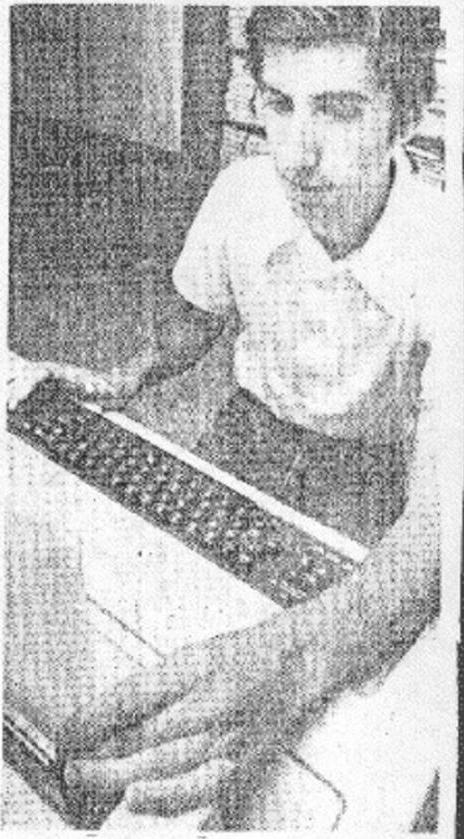
\includegraphics[max width=\textwidth]{2025_03_17_ca60ec0bfd96dcf8e028g-129}
    \caption{My \textenglish{first} \textenglish{attempt} \textenglish{at} \textenglish{mathematical} modeling.}
    \label{fig:first_att_modeling}
\end{figure}

\textbf{\textit{स्टीवन स्कीना}}

...उसकी शुद्धता का परीक्षण करने के लिए\index{data}\index{linear algebra}\index{linear algebra!power of}\index{matrix}\index{Rota, Gian-Carlo}

\section{भविष्यवाणियाँ प्रकाशित}
स्टीवन स्कीना को हर रविवार को \textit{द होम न्यूज़} में एक प्रो फ़ुटबॉल भविष्यवक्ता के रूप में अपनी कौशल दिखाने का मौका मिलेगा।

नवयुवक की साप्ताहिक चयन हमारी फुटबॉल कवरेज में एक "अतिरिक्त घटक" होगा, होम न्यूज़ के कार्यकारी संपादक रॉबर्ट ई. रोड्स के अनुसार।

"मुझे लगता है कि यह हमारे लिए इतना रोचक है कि हमें इसे आजमाना चाहिए," रोड्स ने कहा कि किशोर की कंप्यूटर विधि की मदद से खेलों के परिणाम निर्धारण में क्या होता है। वह एक ईमानदार युवा व्यक्ति लगता है और हम उनके पीछे खड़े रहेंगे।"

स्कीना विजेताओं की भविष्यवाणी करने के लिए एक "साधारण वजीफा" प्राप्त करेंगे, प्रत्येक टीम के लिए स्कोर और अपनी निष्कर्ष के कारण को संक्षेप में समझाने के लिए।

उसका कॉलम पहली बार रविवार के खेल खंड में दिखाई देगा जब नेशनल फुटबॉल लीग (एएफएल) अपना 1977 का सीजन 13 खेलों की स्लेट के साथ खुलता है। स्कीना लीग के सोमवार की रात के खेलों के नतीजे की भविष्यवाणी भी करेंगे।

\textit{होम न्यूज़}खेल अनुभाग में कॉलम प्रकाशित कर रहा है ताकि युवा प्रणाली का परीक्षण किया जा सके और फुटबॉल प्रशंसकों के लिए एक मनोरंजक विशेषता प्रदान की जा सके। इसका उद्देश्य सट्टेबाज़ी को प्रोत्साहित करना नहीं है। "हम उनके चयन को खेल के समय के करीब छापेंगे ताकि सट्टेबाज़ी को रोका जा सके," रोड्स ने कहा। "प्रो फुटबॉल में बड़ी रुचि है और सबसे बढ़कर हम उसकी प्रणाली का परीक्षण करना चाहते हैं। मैं उसके लिए शुभकामनाएं दूंगा।"

\section{एरो का असंभाव्यता प्रमेय}
हमने डेटा से रैंकिंग या स्कोरिंग फंक्शनों के निर्माण के लिए कई दृष्टिकोण देखे हैं। यदि हमारे पास कुछ संस्थाओं के लिए "सही" सापेक्ष क्रम की रिपोर्टिंग करने वाला एक स्वर्ण मानक है, तो इसका उपयोग हमारे स्कोरिंग फंक्शन को इन रैंकिंग के साथ अधिकतम सीमा तक सहमत होने के लिए प्रशिक्षित या मूल्यांकन करने के लिए किया जा सकता है।

लेकिन बिना एक सोने के मानक के, यह दिखाया जा सकता है कि कोई सर्वोत्तम स्‍तरबद्ध प्रणाली नहीं होती। यह \textit{एरो का असंभवता प्रमेय} का परिणाम है, जो यह सिद्ध करता है कि प्राथमिकताओं के क्रमों को संकलित करने वाली कोई भी निर्वाचन प्रणाली निम्नलिखित वांछनीय और निर्दोष-दिखने वाले गुणों को संतुष्ट नहीं करती:

\begin{itemize}
\item प्रणाली को पूर्ण होना चाहिए, जब $A$ और $B$ के बीच विकल्प चुनने के लिए कहा जाए, तो यह कहे कि (1) $A$ को $B$ से प्राथमिकता है, (2) $B$ को $A$ से प्राथमिकता है, या (3) उनके बीच समान प्राथमिकता है। 
\end{itemize}

%---- \textenglish{Page} \textenglish{End} \textenglish{Break} \textenglish{Here} ---- \textenglish{Page} : 114
% Mismatched: \subsectionname{War Story: Who's Bigger?}
\textenglish{My} \textenglish{students} \textenglish{sometimes} \textenglish{tell} \textenglish{me} \textenglish{that} \textenglish{I} \textenglish{am} history. \textenglish{I} \textenglish{hope} \textenglish{this} isn't \textenglish{true} \textenglish{quite} yet, \textenglish{but} \textenglish{I} \textenglish{am} \textenglish{very} \textenglish{interested} \textenglish{in} history, \textenglish{as} \textenglish{is} \textenglish{my} \textenglish{former} \textenglish{postdoc} \textenglish{Charles} Ward. \textenglish{Charles} \textenglish{and} \textenglish{I} \textenglish{got} \textenglish{to} \textenglish{chatting} \textenglish{about} \textenglish{who} \textenglish{the} \textenglish{most} \textenglish{significant} \textenglish{figures} \textenglish{in} \textenglish{history} were, \textenglish{and} \textenglish{how} \textenglish{you} \textenglish{might} \textenglish{measure} this. \textenglish{Like} \textenglish{most} people, \textenglish{we} \textenglish{found} \textenglish{our} \textenglish{answers} \textenglish{in} Wikipedia.

विकिपीडिया एक अद्भुत चीज़ है, एक वितरित कार्य उत्पाद जो 100,000 से अधिक लेखकों द्वारा निर्मित है, जो किसी न किसी रूप में सटीकता और गहराई के सामान्य मानक को बनाए रखता है। विकिपीडिया मानव ज्ञान की एक आश्चर्यजनक मात्रा को एक खुले और यंत्र-पठनीय रूप में संजोता है।

हमने ऐतिहासिक रैंकिंग को आधार बनाने के लिए इंग्लिश विकिपीडिया का उपयोग डेटा स्रोत के रूप में करना शुरू किया। हमारा पहला कदम प्रत्येक व्यक्ति के विकिपीडिया पृष्ठ से फीचर वेरिएबल्स निकालना था जो स्पष्ट रूप से ऐतिहासिक महत्व के साथ संबंध रखते हों। इसमें निम्नलिखित विशेषताएँ शामिल थीं:

\begin{itemize}
  \item \textit{लंबाई:} अधिकांश महत्वपूर्ण ऐतिहासिक व्यक्तित्वों के विकिपीडिया पृष्ठ सामान्य लोगों की तुलना में अधिक लंबे होने चाहिए। इस प्रकार, लेख की शब्दों में लंबाई ऐतिहासिक महत्त्व को कुछ हद तक प्रदर्शित करने वाला एक स्वाभाविक गुण प्रदान करती है।\index{geometry}\index{vectors}\index{vectors!unit}
  \item \textit{हिट्स:} सबसे महत्वपूर्ण व्यक्तित्वों के विकिपीडिया पृष्ठ दूसरों की तुलना में अधिक बार पढ़े जाते हैं, क्योंकि वे अधिक लोगों के लिए अधिक रुचिकर होते हैं। मेरा विकिपीडिया पृष्ठ प्रतिदिन औसतन बीस बार देखा जाता है, जो कि काफी अच्छा है। लेकिन \textenglish{Isaac} \textenglish{Newton} का पृष्ठ प्रतिदिन औसतन 7700 बार देखा जाता है, जो कि कहीं अधिक अच्छा है।
  \item \textit{पेजरैंक:} महत्वपूर्ण ऐतिहासिक व्यक्तित्व अन्य महत्वपूर्ण ऐतिहासिक व्यक्तित्वों के साथ बातचीत करते हैं, जो विकिपीडिया लेखों में हाइपरलिंक संदर्भ के रूप में परिलक्षित होते हैं। यह एक निर्दिष्ट ग्राफ को परिभाषित करता है जहां शिखर लेख होते हैं, और निर्दिष्ट किनार हाइपरलिंक होते हैं। इस ग्राफ का पेजरैंक निकालने पर प्रत्येक ऐतिहासिक व्यक्तित्व की केंद्रीयता मापी जाती है, जो महत्त्व के साथ अच्छी तरह से मेल खाती है।
\end{itemize}

कुल मिलाकर, हमने प्रत्येक ऐतिहासिक व्यक्ति के लिए छह विशेषताओं को निकाला। इसके बाद, हमने इन वेरिएबल्स को समग्रता से पहले सामान्यीकृत किया, मूल रूप से अंतर्निहित रैंकिंग को सामान्य-वितरित वज़नों के साथ मिलाकर, जैसा कि सेक्शन 4.4.2 में सुझाया गया है। हमने\textit{सांख्यिकीय फैक्टर विस्लेषण}नामक तकनीक का प्रयोग किया, जो कि प्रिंसिपल कंपोनेंट एनालिसिस से संबंधित है (सेक्शन 8.5.2 में चर्चा की गई), ताकि दो कारकों को अलग किया जा सके जो हमारे डेटा में सबसे अधिक परिवर्तनशीलता को स्पष्ट करते थे। इन वेरिएबल्स का एक सरल रेखीय संयोजन हमें एक स्कोरिंग फंक्शन देता था, और हमने स्कोर्स को प्रारंभिक रैंकिंग निर्धारित करने के लिए छांटा, जिसे हमने\textit{प्रसिद्धि}कहा।

हमारे मान्यता स्कोर द्वारा शीर्ष बीस आंकड़े चित्र 4.12 (दाईं ओर) में दिखाए गए हैं। हमने इन रैंकिंगों का अध्ययन किया और यह महसूस किया कि यह वास्तव में उस चीज़ को नहीं पकड़ पा रहा था जो हम चाहते थे। मान्यता के हिसाब से शीर्ष बीस में पॉप संगीतकार जैसे मैडोना और माइकल जैक्सन, और तीन समकालीन अमेरिकी राष्ट्रपति शामिल थे। यह स्पष्ट था कि समकालीन आंकड़े अपेक्षा से कहीं अधिक ऊँचे स्थान पर थे: हमारी स्कोरिंग फ़ंक्शन वर्तमान मान्यता को ऐतिहासिक महत्त्व की तुलना में अधिक पकड़ रहा था।

हमारा समाधान समकालीन व्यक्तित्वों के स्कोर को समय के साथ घटाने का था। यह तथ्य कि किसी वर्तमान सेलिब्रिटी को विकिपीडिया पर बहुत सारी हिट्स मिलती हैं, प्रभावशाली है, लेकिन यह अधिक प्रभावशाली है कि हम किसी ऐसे व्यक्ति की अभी भी परवाह करते हैं जो 300 साल पहले मर चुका है। उम्र सुधार के बाद शीर्ष बीस व्यक्तित्व ⸨चित्र 4.12 (बाएँ)⸩ में दिखाए गए हैं।

\begin{center}
\begin{tabular}{c|ccc}
\textenglish{Voter} & \textenglish{Red} & \textenglish{Green} & \textenglish{Blue} \\
\hline
\textenglish{x} & 1 & 2 & 3 \\
\textenglish{y} & 2 & 3 & 1 \\\index{Lincoln, Abraham}\index{matrix!addition}\index{matrix!linear \textenglish{combinations} of}\index{matrix!transpose of}\index{sampling!multiplication}
\textenglish{z} & 3 & 1 & 2 \\
\hline
\end{tabular}
\end{center}

चित्र 4.11: रंगों के लिए पसंदीदा रैंकिंग, जो संक्रमणता के नुकसान को उजागर करती है। लाल को हरे पर तरजीह दी जाती है और हरे को नीले पर, फिर भी नीला लाल पर तरजीह दी जाती है।

\begin{itemize}
  \item परिणाम संक्रामक होने चाहिए, जिसका अर्थ है कि यदि $A$ को $B$ से ज्यादा पसंद किया जाता है, और $B$ को $C$ से ज्यादा पसंद किया जाता है, तो $A$ को $C$ से ज्यादा पसंद किया जाना चाहिए।
  \item अगर हर व्यक्ति $A$ को $B$ से ज्यादा पसंद करता है, तो प्रणाली को $A$ को $B$ से ज्यादा पसंद करना चाहिए।
  \item प्रणाली को केवल एक व्यक्ति, एक तानाशाह, की पसंद पर निर्भर नहीं होना चाहिए।
  \item $A$ की तुलना में $B$ की पसंद किसी अन्य विकल्प, जैसे $C$ की पसंद से स्वतंत्र होनी चाहिए।
\end{itemize}

चित्र 4.11 एरो के प्रमेय के कुछ तत्वों को दर्शाता है, और "रॉक-पेपर-सीज़र्स" प्रकार के क्रम की गैर-पारगम्य प्रकृति को भी प्रदर्शित करता है। यह तीन मतदाताओं (〈x, y〉, और 〈z〉) को उनके पसंदीदा रंगों के बीच रैंकिंग करते हुए दिखाता है। दो रंगों 〈a〉 और 〈b〉 के बीच पसंद को स्थापित करने के लिए, एक तर्कशास्त्रीय प्रणाली यह तुलना कर सकती है कि कितने क्रम 〈a〉 को 〈b〉 से पहले रैंक करते हैं और इसके विपरीत 〈b〉 को 〈a〉 से पहले। इस प्रणाली द्वारा, 〈x〉 और 〈y〉 के अनुसार लाल रंग को हरे रंग पर प्राथमिकता दी जाती है, इसलिए लाल जीतता है। इसी तरह, हरे रंग को नीले रंग पर 〈x〉 और 〈z〉 के द्वारा प्राथमिकता दी जाती है, इसलिए हरा जीतता है। संचरणीयता के अनुसार, इन परिणामों के आधार पर लाल को नीले रंग पर प्राथमिकता दी जानी चाहिए। फिर भी 〈y〉 और 〈z〉 लाल पर नीले को पसंद करते हैं, जो हमारी निर्वाचन प्रणाली से संरक्षित रखने वाले आंतरिक गुण का उल्लंघन करता है।

एरो का प्रमेय बहुत चौंकाने वाला है, लेकिन क्या इसका अर्थ यह है कि हमें डेटा का विश्लेषण करने के उपकरण के रूप में रैंकिंग को छोड़ देना चाहिए? बिल्कुल नहीं, जैसे एरो का प्रमेय यह नहीं कहता कि हमें लोकतंत्र को छोड़ देना चाहिए। जो परंपरागत मतदान प्रणाली बहुमत हुकूमत के विचार पर आधारित होती हैं, वे आम तौर पर लोकप्रिय पसंदों को अच्छी तरह से प्रतिबिंबित करती हैं, विशेष रूप से जब बड़ी संख्या में उम्मीदवारों से निपटने के लिए सही तरीके से सामान्यीकृत किया जाए। और इस अध्याय में तकनीकें आमतौर पर वस्तुओं को दिलचस्प और अर्थपूर्ण तरीकों से रैंक करने का अच्छा काम करती हैं।

\textit{घर ले जाने योग्य पाठ:}हम सही रैंकिंग नहीं खोजते, क्योंकि यह एक अस्पष्ट उद्देश्य है। इसके बजाय, हम ऐसी रैंकिंग खोजते हैं जो उपयोगी और रोचक हों।
%---- पृष्ठ समाप्ति के लिए यहाँ रुकें ---- पृष्ठ : 116

\begin{center}
\begin{tabular}{|r|l|c|l|}\index{associativity}\index{matrix multiplication!applications}
\hline
\textenglish{Signif} & \multicolumn{1}{|c|}{Name} & \multicolumn{1}{|c|}{Fame} & \multicolumn{1}{|c|}{Person} \\
\hline
1 & \textenglish{Jesus} & 1 & \textenglish{George} W. \textenglish{Bush} \\
2 & \textenglish{Napoleon} &  &  \\
3 & \textenglish{William} \textenglish{Shakespeare} & 2 & \textenglish{Barack} \textenglish{Obama} \\
4 & \textenglish{Muhammad} & 3 & \textenglish{Jesus} \\
5 & \textenglish{Abraham} \textenglish{Lincoln} & 4 & \textenglish{Adolf} \textenglish{Hitler} \\
6 & \textenglish{George} \textenglish{Washington} & 5 & \textenglish{Ronald} \textenglish{Reagan} \\
7 & \textenglish{Adolf} \textenglish{Hitler} & 6 & \textenglish{Bill} \textenglish{Clinton} \\
8 & \textenglish{Aristotle} & 7 & \textenglish{Napoleon} \\
9 & \textenglish{Alexander} \textenglish{the} \textenglish{Great} &  &  \\
10 & \textenglish{Thomas} \textenglish{Jefferson} & 8 & \textenglish{Michael} \textenglish{Jackson} \\
11 & \textenglish{Henry} \textenglish{VIII} & 9 & W. \textenglish{Shakespeare} \\
12 & \textenglish{Elizabeth} \textenglish{I} & 10 & \textenglish{Elvis} \textenglish{Presley} \\
13 & \textenglish{Julius} \textenglish{Caesar} & 11 & \textenglish{Muhammad} \\
14 & \textenglish{Charles} \textenglish{Darwin} & 12 & \textenglish{Joseph} \textenglish{Stalin} \\
15 & \textenglish{Karl} \textenglish{Marx} & 13 & \textenglish{Abraham} \textenglish{Lincoln} \\
16 & \textenglish{Martin} \textenglish{Luther} & 14 & G. \textenglish{Washington} \\
17 & \textenglish{Queen} \textenglish{Victoria} & 15 & \textenglish{Albert} \textenglish{Einstein} \\
18 & \textenglish{Joseph} \textenglish{Stalin} & 16 & \textenglish{John} F. \textenglish{Kennedy} \\
19 & \textenglish{Theodore} \textenglish{Roosevelt} &  &  \\
20 & \textenglish{Albert} \textenglish{Einstein} & 17 & \textenglish{Elizabeth} \textenglish{II} \\
 & 18 & \textenglish{John} \textenglish{Paul} \textenglish{II} &  \\
 & 19 & \textenglish{Madonna} &  \\
20 & \textenglish{Britney} \textenglish{Spears} &  &  \\
\hline
\end{tabular}
\end{center}

\begin{figure}[h]
\caption{The \textenglish{top} 20 \textenglish{historical} figures, \textenglish{ranked} \textenglish{by} \textenglish{significance} (\textenglish{left}) \textenglish{and} \textenglish{contemporary} \textenglish{fame} (\textenglish{right}).}
\end{figure}

अब\textit{यह}ही वह था जिसकी हमें तलाश थी! हमने ऐतिहासिक महत्व के लिए जो संभव था, उसका प्रॉक्सी उपयोग करके रैंकिंग को सत्यापित किया: अन्य प्रकाशित रैंकिंग, ऑटोग्राफ कीमतें, खेल सांख्यिकी, इतिहास की पाठ्यपुस्तकें, और हॉल ऑफ फेम चुनाव परिणाम। हमारी रैंकिंग ने इन सभी प्रॉक्सी के खिलाफ एक मजबूत सहसंबंध दर्शाया।

दरअसल, मुझे लगता है कि इन रैंकिंग्स को समझना अद्भुत है। हमनें इनसे सीखे जा सकने वाले सभी प्रकार की चीज़ों का वर्णन करने वाली एक पुस्तक लिखी \cite{SW13}। यदि आपको इतिहास और संस्कृति में रुचि है तो मैं गर्व से आपको इसे पढ़ने के लिए प्रोत्साहित करता हूँ। जितना अधिक हमने इन रैंकिंग्स का अध्ययन किया, उतना ही मैं उनकी सामान्य गुणवत्ता से प्रभावित हुआ।

फिर भी, हमारे प्रकाशित रैंकिंगों ने सार्वभौमिक सहमति नहीं प्राप्त की। बिल्कुल भी नहीं। हमारे रैंकिंग्स के बारे में दर्जनों समाचारपत्र और पत्रिका लेख प्रकाशित हुए, जिनमें से कई काफी शत्रुतापूर्ण थे। लोगों ने उन्हें क्यों नहीं सराहा, भले ही हमने व्यापक सत्यापन किया था? पीछे मुड़कर देखें तो, अधिकतर आलोचना तीन अलग-अलग कारणों से आई:

\begin{itemize}
  \item \textit{महत्व के विभिन्न अप्रत्यक्ष धारणाएं:} हमारे तरीकों को \textit{मीम-ताकत} मापने के लिए डिज़ाइन किया गया था, जो यह जांचने में सक्षम थे कि ये ऐतिहासिक व्यक्ति अपने नामों को इतिहास में कितना सफलतापूर्वक फैला रहे थे। लेकिन कई पाठकों का मानना था कि हमारे तरीकों को ऐतिहासिक \textit{महानता} का भी माप करना चाहिए। कौन सबसे महत्वपूर्ण था, दुनिया को बदलने के मामले में? और क्या हम दुनिया की बात कर रहे हैं या केवल अंग्रेजी-भाषी दुनिया की? जब वे दुनिया की आबादी के 30 \%$ से अधिक का प्रतिनिधित्व करते हैं, तब सूची में कोई चीनी या भारतीय व्यक्ति कैसे नहीं हो सकता?\\
हमें मापने से पहले यह तय करना होगा कि हम क्या मापने की कोशिश कर रहे हैं। ऊँचाई आकार का एक उत्कृष्ट माप है, लेकिन यह मोटापे का अच्छा माप नहीं है। हालांकि, ऊँचाई बास्केटबॉल टीम के लिए खिलाड़ियों का चयन करने में बहुत उपयोगी है।
  $ \textit{अलगाव:} \index{outlier}नज़र टेस्ट किसी विश्लेषण के परिणामों का मूल्यांकन करने के लिए महत्वपूर्ण हैं। हमारी रैंकिंग के बारे में यह उन लोगों के स्थान की जांच करना था जिन्हें हम जानते थे, यह सुनिश्चित करने के लिए कि वे उचित स्थानों पर हैं।\\\index{matrix!adjacency}\index{matrix!identity}\index{paths}\index{permutation}
हमारे तरीकों की रैंकिंग के अनुसार अधिकांश ऐतिहासिक महान व्यक्तियों के बारे में मुझे बहुत अच्छा महसूस हुआ। लेकिन कुछ ऐसे थे जिन्हें हमारे तरीकों ने किसी भी समीचीन व्यक्ति से अधिक उच्च स्थान दिया, विशेष रूप से राष्ट्रपति जॉर्ज डब्ल्यू. बुश (36) और किशोर टीवी स्टार हिलेरी डफ (1626)। कोई इन अलगावों को देखकर संपूर्ण चीज को अस्वीकार कर सकता है। लेकिन समझिए कि हमने लगभग 850,000 ऐतिहासिक महान व्यक्तियों को रैंक किया, जो लगभग सैन फ्रांसिस्को की आबादी के बराबर है। कुछ चुनिंदा गलत उदाहरणों को सही संदर्भ में डालना होगा।
  \item \textit{पिजनहोल बाधाएं:} अधिकांश समीक्षकों ने केवल हमारे शीर्ष 100 व्यक्तियों की रैंकिंग देखी, और उन्होंने विशेष रूप से यह शिकायत की कि हमने लोगों को कहां रखा है और कौन कटौती नहीं कर पाया। महिलाओं के टीवी शो \textit{द व्यू} ने शिकायत की कि हमने पर्याप्त महिलाएं नहीं रखीं। मुझे ब्रिटिश लेख याद हैं जिन्होंने शिकायत की थी कि हमने विंस्टन चर्चिल (37) को बहुत नीचे रैंक दिया, दक्षिण अफ्रीकी लेख जिन्होंने सोचा कि हमने नेल्सन मंडेला (356) को कम आंका, चीनी लेख जिन्होंने कहा कि हमारे यहाँ पर्याप्त चीनी नहीं हैं, और यहां तक कि एक चिली पत्रिका जिसने चिलीवासी की अनुपस्थिति के बारे में शिकायत की।\\
इनमें से कुछ संस्कृतिगत अंतर को दर्शाता है। इन आलोचकों के पास अंग्रेजी विकिपीडिया द्वारा दर्शाए गए महत्व की अवधारणा से अलग एक वाह्य धारणा थी। लेकिन इसमें से बहुत कुछ इस तथ्य को दर्शाता है कि शीर्ष 100 में केवल एक सौ स्थान होते हैं। कई व्यक्ति जिन्हें वे गायब मानते थे, वे केवल दृश्य क्षितिज के थोड़ा ही बाहर थे। हर नए व्यक्ति को जो हमने शीर्ष सौ में स्थानांतरित किया, हमें किसी और को बाहर करना पड़ा। लेकिन पाठक शायद ही कभी उन नामों का सुझाव देते हैं जिन्हें हटाना चाहिए, केवल उन्हीं का जिन्हें जोड़ा जाना चाहिए।
\end{itemize}

इसके पीछे नैतिक क्या है? अपने रैंकिंग के लिए दर्शकों की चिंताओं का पूर्वानुमान लगाने की कोशिश करें। हमें प्रोत्साहित किया गया था कि हम अपने माप को स्पष्ट रूप से\textit{मेम-स्ट्रेंग्थ}कहें\textit{महत्व}के बजाय। पीछे मुड़कर देखने पर, इस कम-भरे हुए नाम का उपयोग हमारे पाठकों को यह समझने की अनुमति देता कि हम क्या कर रहे थे। शायद हमें अपने पाठकों को हमारी शीर्ष 100 रैंकिंग पर टिकने से भी हतोत्साहित करना चाहिए था, और इसके बजाय रुचि समूहों के भीतर सापेक्ष क्रमों पर ध्यान केंद्रित करना चाहिए: शीर्ष संगीतकार, वैज्ञानिक, और कलाकार कौन थे? यह कम विवादास्पद साबित हो सकता था, जिससे लोग हमारे काम पर विश्वास करना बेहतर समझ पाते।\index{matrix!identity}\index{matrix!inversion}\index{matrix!rotation}\index{point spread!rotating}

\section{अध्याय नोट्स}
लैंगविले और मेयर \cite{langville2012who} यहां पर चर्चा किए गए अधिकांश रैंकिंग विधियों, जिसमें \textenglish{Elo} और \textenglish{PageRank} शामिल हैं, का विस्तृत परिचय प्रदान करते हैं।

%---- \textenglish{Page} \textenglish{End} \textenglish{Break} \textenglish{Here} ---- \textenglish{Page} : 118

इस अध्याय में एक महत्वपूर्ण विषय शामिल नहीं है \textit{रैंक करने की विधियाँ सीखना}, जो उपयुक्त स्कोरिंग कार्यों को प्रशिक्षित करने के लिए स्वर्ण मानक रैंकिंग डेटा का उपयोग करती हैं। ऐसा आधार-तथ्य डेटा सामान्यतः उपलब्ध नहीं होता, लेकिन कभी-कभी इसके उपप्रकार मिल सकते हैं। जब खोज इंजन का मूल्यांकन किया जाता है, तो उपयोगकर्ता द्वारा (मान लें) उन्हें प्रस्तुत चौथी वस्तु पर क्लिक किए जाने की टिप्पणी को इस रूप में व्याख्या की जा सकती है कि इसे पहले रखी गई तीन वस्तुओं से उच्च रैंक मिलनी चाहिए थी। एसवीएमरैंक \cite{joachims2002optimizing} ऐसे डेटा से रैंकिंग कार्यों को सीखने की एक विधि प्रस्तुत करता है।

प्रस्तावित हीयूरिस्टिक एक शीर्षक क्रम में किनारा संघर्षों को न्यूनतम करने के लिए \textenglish{Eades} और उनके सहकर्मियों द्वारा दी गई है \cite{eades1993fast}. एरो की असंभवता प्रमेय का मेरा प्रस्तुतीकरण \textenglish{Watkins} के नोट्स पर आधारित है \cite{watkins2016arrow}.

इस अध्याय की युद्ध कहानियाँ मेरे पुस्तकों\textit{Calculated Bets}और\textit{Who's Bigger?}से बहुत करीब से ली गई हैं। मुझे आत्म-नकल के लिए मुकदमा मत कीजिए।

\section{व्यायाम}
% मेल नहीं खाता: \subsectionname{स्कोर्स और रैंकिंग्स}

\begin{enumerate}
  \item मान लीजिए \(X\) एक यादृच्छिक चर को प्रदर्शित करता है जो सामान्य वितरण से लिया गया है, परिभाषित \( \mu=2 \) और \( \sigma=3 \) के द्वारा है। मान लीजिए कि हम \( X=5.08 \) का अवलोकन करते हैं। \( \textenglish{x} \) का Z-स्कोर खोजें, और यह निर्धारित करें कि \( \textenglish{x} \) माध्य से कितने मानक विचलन दूर है। 
  \item मानक सामान्य वितरण \(( \mu=0, \sigma=1 )\) का कितना प्रतिशत प्रत्येक क्षेत्र में पाया जाता है? 
    \begin{enumerate}
      \item \(Z>1.13\).\index{Gates, Bill!elimination}\index{linear systems}
      \item \(Z<0.18\).
      \item \(Z>8\).
      \item \(|Z|<0.5\).
    \end{enumerate}

\itemअमांडा ने ग्रैजुएट रेकॉर्ड एग्जामिनेशन (जीआरई) दिया, और 160 अंक प्राप्त किए मौखिक तर्क और 157 अंक मात्रात्मक तर्क में। मौखिक तर्क के लिए औसत स्कोर 151 था जिसमें मानक विचलन 7 था, जबकि मात्रात्मक तर्क के लिए औसत\(\mu=153\)और\(\sigma=7.67\)था। मानें कि दोनों वितरण सामान्य हैं।

\begin{enumerate}
      \item अमांडा के इन परीक्षा अनुभागों में Z-स्कोर क्या थे? इन स्कोर को एक मानक सामान्य वितरण वक्र पर चिह्नित करें।
      \item उसने अन्य विद्यार्थियों की तुलना में किस अनुभाग में बेहतर प्रदर्शन किया?
      \item इन दो परीक्षाओं के लिए उसके पर्सेंटाइल स्कोर का पता लगाएं।
    \end{enumerate}

\itemअपने व्यक्तिगत रुचि के क्षेत्रों में तीन सफल और अच्छी तरह से उपयोग की जाने वाली स्कोरिंग फंक्शन को पहचानें। प्रत्येक के लिए, यह समझाएँ कि इसे एक अच्छी स्कोरिंग फंक्शन क्या बनाती है और यह दूसरों द्वारा कैसे उपयोग की जाती है।
\itemनिम्नलिखित वर्गों की चीजों में से किसी एक की विशेषताओं पर डेटा सेट खोजें:

\begin{enumerate}
      \item दुनिया के देश.
      \item फिल्में और फिल्म सितारे.
      \item खेल सितारे.
      \item विश्वविद्यालय.
    \end{enumerate}

गुणवत्ता या लोकप्रियता को दर्शाने वाला एक समझदार रैंकिंग फ़ंक्शन निर्माण करें। यह किस हद तक किसी बाहरी माप के साथ मेल खाता है जो समान परिणाम को लक्षित कर रहा है? 
\itemउसी वस्तुओं के सेट पर दो मौलिक रूप से भिन्न लेकिन समझदार स्कोरिंग फ़ंक्शन तैयार करें। परिणामस्वरूप रैंकिंग कितनी अलग हैं? क्या यह तथ्य कि दोनों को समझदार होना चाहिए, रैंकिंग को प्रमुख रूप से समान बनाता है? 
\itemव्यावसायिक खेल लीग्स द्वारा सबसे मूल्यवान खिलाड़ी पुरस्कार विजेता का चयन करने के लिए उपयोग किए जाने वाले स्कोरिंग सिस्टम आमतौर पर मतदाताओं द्वारा निर्दिष्ट क्रमपरिवर्तन को स्थितिक वज़न आवंटित करते हैं। वे पेशेवर बेसबॉल, बास्केटबॉल, और फुटबॉल में कौन से सिस्टम का उपयोग करते हैं? क्या वे समान हैं? क्या आपको लगता है कि वे समझदार हैं? 
\end{enumerate}

\subsection{कार्यान्वयन परियोजनाएँ}

\begin{enumerate}
  \item \textenglish{Elo} रेटिंग्स का उपयोग करके बेसबॉल, फुटबॉल, या बास्केटबॉल जैसे खेल में सभी टीमों की रैंकिंग करें, जो प्रत्येक नए खेल के परिणाम के अनुसार रेटिंग समायोजित करता है। भविष्य की प्रतियोगिताओं के परिणामों की भविष्यवाणी ये \textenglish{Elo} रेटिंग्स कितनी सटीकता से करती हैं?
  \item Borda’s विधि की मजबूती का मूल्यांकन करें \(p=\{1,2, \ldots, n\}\) क्रम के \(m\) अलग-अलग प्रतियों में प्रत्येक को \(k\) रैंडम स्वैप्स लागू करके। वह कौन सा सीमा है जहाँ Borda’s विधि \(p\) को फिर से बनाने में विफल रहती है, \(n, k,\) और \(m\) के फ़ंक्शन के रूप में?
\end{enumerate}

\subsection{साक्षात्कार प्रश्न}

\begin{enumerate}
  \item क्या चीज एक डेटा सेट को एक स्वर्ण मानक बनाती है?
  \item आप कैसे जाँच सकते हैं कि नया क्रेडिट जोखिम स्कोरिंग मॉडल काम करता है या नहीं?
  \item आप अमेज़ॅन सार्वजनिक डेटा के आधार पर किसी विशेष पुस्तक के लिए बिक्री का पूर्वानुमान कैसे लगाएंगे?
\end{enumerate}

\subsection{कागल चैलेंज}

\begin{enumerate}
  \item खेल स्थिति से चेस खिलाड़ियों की रेटिंग। \url{https://www.kaggle.com/c/chess}\index{Gray, Dorian}
  \item एक वित्तीय क्रेडिट स्कोरिंग प्रणाली विकसित करें। \url{https://www.kaggle.com/c/GiveMeSomeCredit}
  \item विज्ञापन से नौकरी के वेतन की भविष्यवाणी करें। \url{https://www.kaggle.com/c/job-salary-prediction}\index{matrix!factoring}\index{matrix!reasons \textenglish{for} factoring}
\end{enumerate}

\chapter{सांख्यिकीय विश्लेषण}

\textit{सांख्यिकी के साथ झूठ बोलना आसान है, लेकिन उनके बिना झूठ बोलना और भी आसान है।}

\begin{flushright}
 -- फ्रेडरिक मोस्टेलर
\end{flushright}

मैं स्वीकार करूँगा कि मैंने कभी भी एक सांख्यिकीविद् के साथ वास्तव में संतोषजनक बातचीत नहीं की है। यह पूरी तरह से प्रयास की कमी के कारण नहीं है। कई बार वर्षों के दौरान मैंने सांख्यिकीविदों की रुचि के समस्याओं को लिया है, लेकिन हमेशा उत्तर लेकर वापस आया हूँ जैसे "आप इसे इस तरह नहीं कर सकते" या "लेकिन यह स्वतंत्र नहीं है," बजाय इसके कि सुनने को मिले "इसे संभालने का यह तरीका है।"

सच्चाई यह है कि, ये सांख्यिकीविद भी सामान्यतः मेरे साथ बातचीत करने की सराहना नहीं करते थे। सांख्यिकीविद डेटा के बारे में कंप्यूटर वैज्ञानिकों से कहीं अधिक समय से गंभीरता से सोचते आ रहे हैं, और उनके पास इसे प्रदर्शित करने के लिए कई शक्तिशाली विधियाँ और विचार हैं। इस अध्याय में, मैं इन महत्वपूर्ण उपकरणों में से कुछ का परिचय दूंगा, जैसे कि कुछ मौलिक वितरणों की परिभाषाएँ और सांख्यिकीय महत्व के परीक्षण। यह अध्याय बायज़ियन विश्लेषण का भी परिचय देगा, जो एक तरीका है कि नई डेटा कैसे हमारे भविष्य की घटनाओं के पूर्वानुमानों को प्रभावित करना चाहिए, इसका सख्ती से आकलन किया जा सकता है।

\begin{figure}
  \centering
  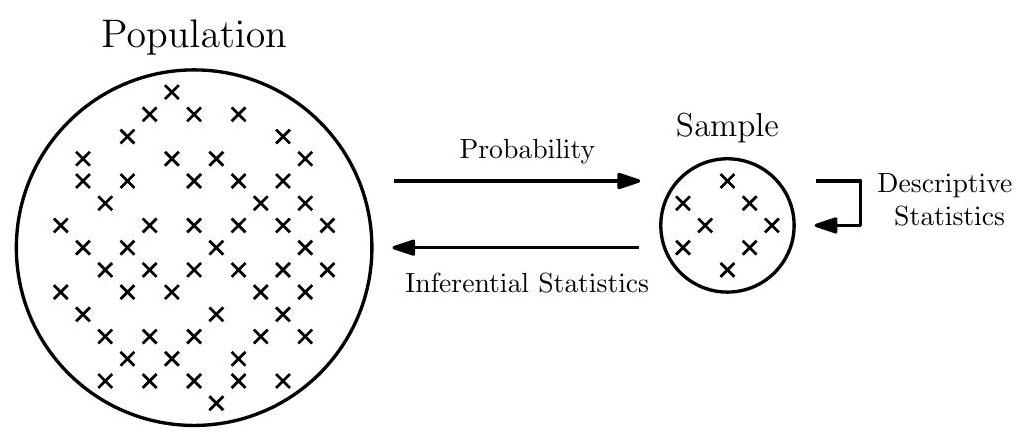
\includegraphics[max width=\textwidth]{2025_03_17_ca60ec0bfd96dcf8e028g-137}
  \caption{The \textenglish{central} \textenglish{dogma} \textenglish{of} statistics: \textenglish{analysis} \textenglish{of} \textenglish{a} \textenglish{small} \textenglish{random} \textenglish{sample} \textenglish{enables} \textenglish{drawing} \textenglish{rigorous} \textenglish{inferences} \textenglish{about} \textenglish{the} \textenglish{entire} population.}
\end{figure}

फ़िगर 5.1 सांख्यिकीय तर्क प्रक्रिया को दर्शाता है। संभावित वस्तुओं की एक अंतर्निहित जनसंख्या होती है जिसे हम संभवतः देख सकते हैं। वास्तव में केवल उनका एक अपेक्षाकृत छोटा उपसमूह होता है जिसे हल्के रूप से यादृच्छिक रूप से नमूना लिया जाता है, जिसका अर्थ है कि हम नमूने की गई वस्तुओं के गुणों का अवलोकन कर सकते हैं। प्रायिकता सिद्धांत वर्णन करता है कि हमारे नमूने के क्या गुण होने चाहिए, यह दिए गए अंतर्निहित जनसंख्या के गुणों द्वारा निर्धारित होता है। लेकिन\textit{सांख्यिकीय अनुमान}विपरीत दिशा में कार्य करता है, जहां हम नमूने के विश्लेषण के आधार पर पूरी जनसंख्या कैसी है, इसका अनुमान लगाने का प्रयास करते हैं।

आदर्श रूप से, हम एक सांख्यिकीविद् की तरह सोचना सीखेंगे: इतना कि सतर्क रहें और अति-व्याख्या और त्रुटियों से बचें, जबकि डेटा के साथ खेलने और उसे जहाँ ले जाता है, वहाँ ले जाने का आत्मविश्वास बनाए रखें।

\section{सांख्यिकीय वितरण}
हर परिवर्तनीय जो हम निरीक्षण करते हैं, एक विशेष आवृत्ति वितरण को परिभाषित करता है, जो यह दर्शाता है कि प्रत्येक विशेष मान कितनी बार आता है। ऊँचाई, वजन, और \textenglish{IQ} जैसी परिवर्तनीयों की अद्वितीय विशेषताएँ उनके वितरणों द्वारा अभिव्यक्त की जाती हैं। लेकिन इन वितरणों के आकार स्वयं अद्वितीय नहीं होते: बड़ी हद तक, दुनिया की समृद्ध डेटा विविधता केवल कुछ क्लासिकल रूपों में प्रकट होती है।

ये शास्त्रीय वितरणों में दो अच्छी विशेषताएँ होती हैं: (1) ये आवृत्ति वितरण के आकारों का वर्णन करती हैं जो व्यवहार में अक्सर उत्पन्न होती हैं, और (2) इन्हें अक्सर बहुत कम पैरामीटरों के साथ बंद-आकृति अभिव्यक्तियों का उपयोग करते हुए गणितीय रूप से वर्णित किया जा सकता है। जब विशिष्ट डेटा टिप्पणियों से अमूर्त कर ली जाती हैं, तब ये \textit{संभाव्यता वितरण} बन जाती हैं, जो स्वतंत्र अध्ययन के योग्य होती हैं।

शास्त्रीय प्रायिकता वितरणों की जानकारी महत्वपूर्ण है। वे अक्सर व्यवहार में आते हैं, इसलिए आपको इन पर नज़र रखनी चाहिए। ये हमें यह बात करने की शब्दावली देते हैं कि हमारे डेटा का स्वरूप कैसा होता है। हम आने वाले खंडों में सबसे महत्वपूर्ण सांख्यिकी वितरणों (बाइनॉमियल, नॉर्मल, पोआसोन, और पावर लॉ) की समीक्षा करेंगे, उनके गुणों पर जोर देते हुए जो उनके आवश्यक चरित्र को परिभाषित करते हैं।\index{eigenvalues}\index{eigenvalues!properties of}\index{matrix!eigenvalues}\index{matrix!eigenvectors}

ध्यान दें कि आपका देखा गया डेटा किसी विशेष सैद्धांतिक वितरण से उत्पन्न नहीं होता केवल इसलिए कि उसका आकार समान है। सांख्यिकी परीक्षणों का उपयोग यह कठोरता से प्रमाणित करने के लिए किया जा सकता है कि क्या आपका प्रायोगिक रूप से देखा गया डेटा किसी विशेष वितरण से लिए गए नमूनों को दर्शाता है।\index{LU decomposition}\index{matrix!determinant}\index{matrix!triangular}\index{word embeddings}

लेकिन मैं आपको इनमें से किसी भी परीक्षण को वास्तव में चलाने की परेशानी से बचाने जा रहा हूँ। मैं पूरे विश्वास के साथ कह सकता हूँ कि आपका वास्तविक-विश्व डेटा\textit{ठीक से}किसी भी प्रसिद्ध सैद्धांतिक वितरितियों के अनुरूप नहीं है।

ऐसा क्यों होता है? समझें कि दुनिया एक जटिल जगह है, जो इसे मापने की प्रक्रिया को एक उलझा हुआ कार्य बना देती है। आपकी टिप्पणियाँ शायद कई नमूना जनसंख्याओं से ली जाएँगी, जिनमें से प्रत्येक का कुछ भिन्न आधारभूत वितरण होता है। सामान्यतः किसी भी देखी गई वितरण के सिरों पर कुछ हास्यात्मक होता है: असामान्य रूप से उच्च या निम्न मूल्यों का अचानक उछाल। मापों के साथ त्रुटियाँ जुड़ी होती हैं, कभी-कभी विचित्र प्रणालीगत तरीकों में।

लेकिन यह कहा गया, मूलभूत वितरणों को समझना वास्तव में बहुत महत्वपूर्ण है। प्रत्येक शास्त्रीय वितरण किसी कारणवश शास्त्रीय है। इन कारणों को समझना आपको देखे गए डेटा के बारे में बहुत कुछ बताता है, इसलिए उन्हें यहाँ पर समीक्षा की जाएगी।

%---- \textenglish{Page} \textenglish{End} \textenglish{Break} \textenglish{Here} ---- \textenglish{Page} : 122



\begin{figure}[H]
    \centering
    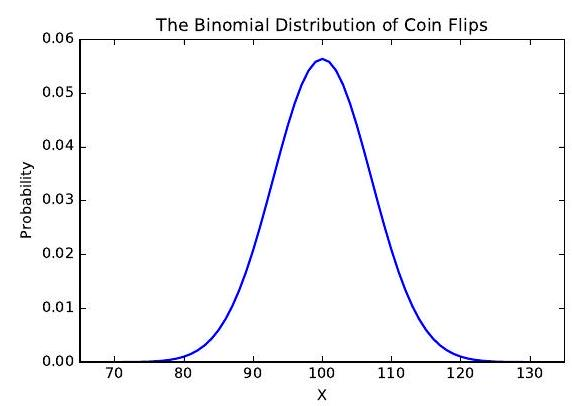
\includegraphics[max width=\textwidth]{2025_03_17_ca60ec0bfd96dcf8e028g-139(1)}
    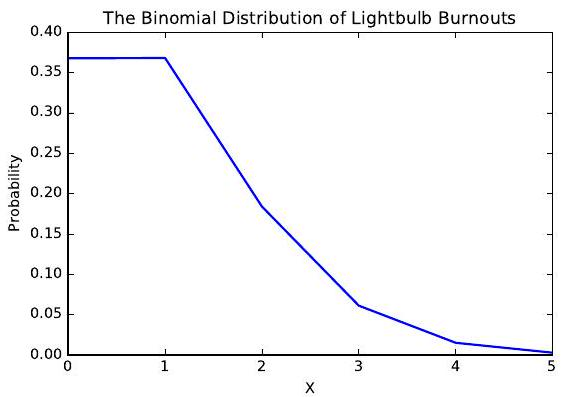
\includegraphics[max width=\textwidth]{2025_03_17_ca60ec0bfd96dcf8e028g-139}
    \caption{The \textenglish{binomial} \textenglish{distribution} \textenglish{can} \textenglish{be} \textenglish{used} \textenglish{to} \textenglish{model} \textenglish{the} \textenglish{distribution} \textenglish{of} \textenglish{heads} \textenglish{in} 200 \textenglish{coin} \textenglish{tosses} \textenglish{with} $p=0.5$ (\textenglish{left}), \textenglish{and} \textenglish{the} \textenglish{number} \textenglish{of} \textenglish{blown} \textenglish{lightbulbs} \textenglish{in} 1000 \textenglish{events} \textenglish{with} \textenglish{failure} \textenglish{probability} $p=0.001$ (\textenglish{right}).}
\end{figure}

\subsection{द्विपद वितरण}
एक प्रयोग पर विचार करें जिसमें समान, स्वतंत्र परीक्षण शामिल होते हैं, जिनके दो संभव परिणाम होते हैं$P_1$और$P_2$, जिनकी संभावना क्रमशः$p$और$q=(1-p)$होती है। आपका प्रयोग शायद सिक्के उछालना हो सकता है, जहां सिर आने की संभावना$(p=0.5)$पूंछ आने की संभावना$(q=0.5)$के समान होती है। शायद यह बार-बार लाइट स्विच चालू करना हो, जहां बल्ब बदलना पड़ने का अचानक पता चलने की संभावना($p=0.001$) लाइट जलने की संभावना ($q=0.999$) से बहुत कम होती है।

बाइनोमियल वितरण ठीक$x P_1$घटनाओं को$n$स्वतंत्र परीक्षणों के दौरान प्राप्त करने की संभावना को रिपोर्ट करता है, बिना किसी विशेष क्रम के। स्वतंत्रता यहाँ महत्वपूर्ण है: हम मानते हैं कि बल्ब के फेल होने की संभावना का कोई संबंध नहीं है कि इसे पहले कितनी बार इस्तेमाल किया गया है। बाइनोमियल वितरण के लिए पीडीएफ को निम्नलिखित द्वारा परिभाषित किया गया है:

\begin{equation}
P(X=x)=\binom{n}{x} p^{x}(1-p)^{(n-x)}
\end{equation}

बाइनोमियल डिस्ट्रीब्यूशन के बारे में कई बातें ध्यान देने योग्य हैं:

\begin{itemize}
    \item \textit{यह असतत है}: बाइनॉमियल वितरण के दोनों तर्क ($n$ और $x$) पूर्णांक होने चाहिए। चित्र \ref{fig:binomial} (बाएँ) की चिकनाई एक भ्रांति है, क्योंकि $n=200$ काफी बड़ा है। 200 सिक्के उछालने पर 101.25 हेड्स प्राप्त करने का कोई तरीका नहीं है।
    \item \textit{आप शायद इसके पीछे का सिद्धांत समझा सकते हैं}: आपने हाई स्कूल में पहली बार बाइनॉमियल वितरण का सामना किया था। याद है पास्कल का त्रिभुज? $n$ उछालों में ठीक $x$ हेड्स प्राप्त करने का संभावना $p^{x}(1-p)^{(n-x)}$ होती है, प्रत्येक $\binom{n}{x}$ अलग-अलग उछाल क्रम के लिए।
    \item \textit{यह कुछ-कुछ घंटी के आकार का है}: एक निष्पक्ष सिक्के के लिए $(p=0.5)$, बाइनॉमियल वितरण पूरी तरह से सममित है, और माध्य मध्य में होता है। यह बल्ब के मामले में सत्य नहीं है: यदि हम केवल $n=1000$ बार बल्ब चालू करते हैं, तो विफलताओं की सबसे संभावित संख्या शून्य होगी। यह चित्र \ref{fig:binomial} में सिर्फ आधी घंटी बजाता है। इतना कहा गया, जैसे-जैसे $n\rightarrow बढेगा, हम माध्य में चोटी वाले एक सममित वितरण को प्राप्त करेंगे।
    \infty \textit{यह केवल दो मापदंडों का उपयोग करके परिभाषित किया गया है}: हमें केवल $p\item और $n$ के मानों की आवश्यकता होती है ताकि दी गई बाइनॉमियल वितरण को पूरी तरह से परिभाषित किया जा सके।
\end{itemize}

कई चीजों को ठीक से बायनॉमियल वितरण द्वारा मॉडल किया जा सकता है। अनुभाग 2.2.3 में चर्चा किए गए एक$p=0.300$हिटर के प्रदर्शन में बदलाव को याद करें। वहां प्रत्येक प्रयास में हिट मिलने की संभावना$p=0.3$थी, और प्रति सीजन$n=500$प्रयास होते थे। इस प्रकार प्रति सीजन मिलने वाले हिटों की संख्या बायनॉमियल वितरण से खींची गई है।

यह महसूस करते हुए कि यह एक बाइनोमियल वितरण था, इसका मतलब था कि वास्तव में हमें वितरण बनाने के लिए सिमुलेशन का उपयोग करने की आवश्यकता नहीं थी। उम्मीद की गई हिट्स की संख्या जैसे गुण $=n p=500\mu0.3=150\times और इसका मानक विचलन 
$
\[=\sqrt{n \textenglish{p} q}=\sqrt{500 \sigma 0.3 \times 0.7}= 10.25 
\times
बंद रूप के सूत्रों से प्राप्त होते हैं जिन्हें आप आवश्यकतानुसार देख सकते हैं।

\subsection{सामान्य वितरण}
\index{normal distribution}बहुत से प्राकृतिक घटनाएं जिनकी गणना घंटी के आकार के वक्रों द्वारा की जाती है। मापी गई विशेषताएं जैसे कि ऊँचाई, वजन, जीवनकाल, और आईक्यू सभी एक ही मूल योजना के अंतर्गत आते हैं: मूल्यों का बड़ा हिस्सा औसत के बहुत करीब होता है, वितरण सममित होता है, और कोई भी मूल्य अत्यधिक नहीं होता। दुनिया के पूरे इतिहास में, न तो कभी एक 12 फुट लंबा आदमी हुआ है और न ही कोई 140 साल की महिला।

सभी घंटी के आकार के वक्रों की जननी\textit{गौसियन}या\textit{सामान्य वितरण}है, जो पूरी तरह से इसके औसत और मानक विचलन द्वारा संयोजित होती है:

\begin{equation}
P(\textenglish{x})=\frac{1}{\sigma \sqrt{2 \pi}} e^{-(x-\mu)^{2} / 2 \sigma^{2}}
\end{equation}

\begin{figure}[H]
    \centering
    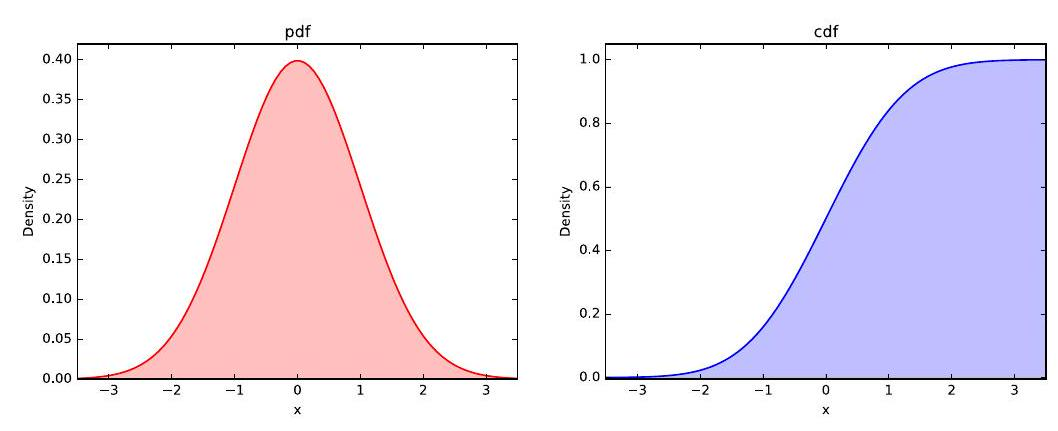
\includegraphics[max width=\textwidth]{2025_03_17_ca60ec0bfd96dcf8e028g-140}
    \caption{The \textenglish{probability} \textenglish{density} \textenglish{function} (\textenglish{pdf}) \textenglish{of} \textenglish{the} \textenglish{normal} \textenglish{distribution} (\textenglish{left}) \textenglish{with} \textenglish{its} \textenglish{corresponding} \textenglish{cumulative} \textenglish{density} \textenglish{function} (\textenglish{cdf}) \textenglish{on} right.}
\end{figure}

यहाँ कई बातें ध्यान देने योग्य हैं:

\begin{itemize}
    \item \textit{यह सतत है}: सामान्य वितरण के तर्क (औसत $\mu$ और मानक विचलन $\sigma$) मनमाने वास्तविक संख्याओं में स्वतंत्र होते हैं, केवल यह एकल बाधा है कि $\sigma>0$।
    \item \textit{आप शायद यह नहीं समझा सकते कि यह कहां से आता है}: सामान्य वितरण द्विपद वितरण का सामान्यीकरण है, जहां $n \rightarrow \infty$ और औसत के आसपास की एकाग्रता की डिग्री को पैरामीटर $\sigma$ द्वारा निर्दिष्ट किया जाता है। यहाँ अपने अंतर्ज्ञान को द्विपद वितरण से लें, और विश्वास करें कि गॉस ने अपनी गणना सही की है: महान गणितज्ञ ने सामान्य वितरण को अपने पीएच.डी. शोध प्रबंध के लिए तैयार किया। या यदि आप वास्तव में उत्सुक हैं, तो देख सकते हैं कि यह कहां से आता है, किसी भी अच्छे सांख्यिकी पुस्तक से परामर्श करें।
    \item \textit{यह वास्तव में घंटी के आकार का है}: गॉसियन वितरण \index{Gaussian distribution} घंटी के आकार की वक्र का प्लेटोनिक उदाहरण है। क्योंकि यह एक सतत चर (जैसे, ऊँचाई) पर काम करता है, बजाय किसी विषम गणना (जैसे, घटनाओं की संख्या) के, यह पूर्णतः गौण है। क्योंकि यह दोनों दिशाओं में अनंत जाता है, इसके अंत में तनों की कोई कटौती नहीं होती। सामान्य वितरण एक सैद्धांतिक निर्माण है, जो इस पूर्णता को समझाने में मदद करता है।\index{principal components}\index{principal components!analysis}
    \item \textit{यह केवल दो पैरामीटर का उपयोग करके परिभाषित होता है}: हालांकि, ये पैरामीटर द्विपद वितरण से भिन्न हैं! सामान्य वितरण पूरी तरह से अपने केंद्रीय बिंदु (जो औसत $\mu$ द्वारा दिया जाता है) और उसके फैलाव (जो मानक विचलन $\sigma$ द्वारा दिया जाता है) द्वारा परिभाषित होता है। वे केवल वही कुञ्जियाँ हैं जो हम वितरण को समायोजित करने के लिए उपयोग कर सकते हैं।
\end{itemize}

\section{सामान्य क्या है?}

बहुत सारे प्राकृतिक रूप से घटित होने वाले घटनाक्रमों का माॅडल सामान्य वितरण द्वारा बनाया जाता है। शायद सबसे महत्वपूर्ण एक है मापन त्रुटि। जब भी आप बाथरूम स्केल पर अपना वजन मापते हैं, तो आपको थोड़ा भिन्न उत्तर मिलेगा, भले ही आपका वजन न बदला हो। कभी-कभी स्केल ऊँचा दिखाएगा और कभी-कभी कम, यह कमरे के तापमान और फर्श के टेढ़ापन पर निर्भर करता है। छोटे त्रुटियों की संभावना बड़ी त्रुटियों की तुलना में अधिक होती है, और थोड़ा ऊँचा या थोड़ा कम होने की संभावना बराबर होती है। प्रायोगिक त्रुटि को सामान्यतः\textit{गॉसियन शोर} के रूप में वितरित किया जाता है।

भौतिक परिघटनाएँ जैसे ऊँचाई, वजन, और जीवनकाल सभी की घंटी के आकार की प्राप्तियाँ होती हैं, समान तर्कों द्वारा। फिर भी, यह दावा कि ऐसी प्राप्तियाँ \textit{सामान्य} हैं, अक्सर बहुत आसानी से किया जाता है, बिना सही तरीके से अधीनस्थ जनसंख्या को निर्दिष्ट किए। क्या मानव ऊँचाई सामान्य रूप से वितरित होती है? निश्चित रूप से नहीं: पुरुषों और महिलाओं की औसत ऊँचाई और संबंधित वितरण अलग-अलग होते हैं। क्या पुरुषों की ऊँचाई सामान्य रूप से वितरित होती है? निश्चित रूप से नहीं: बच्चों को शामिल करके और वृद्ध नागरिकों की ऊँचाई घटाकर, आपके पास फिर से कई अलग-अलग अधीनस्थ वितरणों का योग हो जाता है। क्या संयुक्त राज्य अमेरिका में वयस्क पुरुषों की ऊँचाई सामान्य है? नहीं, शायद तब भी नहीं। ऐसी गैर-तुच्छ जनसंख्या है जिनमें वृद्धि विकार जैसे बौनापन और एक्रोमेगेली हैं, जो सामान्य वितरण द्वारा समझाई जा सकने की तुलना में लोगों को काफी छोटा और लंबा बनाते हैं।

शायद सबसे प्रसिद्ध घंटी के आकार वाला लेकिन गैर-सामान्य वितरण वित्तीय बाजारों में दैनिक रिटर्न (प्रतिशत मूल्य हरकतों) का है। एक बड़े बाजार दुर्घटना को एक बड़े प्रतिशत मूल्य गिरावट से परिभाषित किया जाता है: 10 अक्टूबर, 1987 को, डॉव जोन्स औसत ने अपने मूल्य का 22.61% खो दिया। बड़े स्टॉक बाजार दुर्घटनाएँ सामान्य वितरण द्वारा सही ढंग से मॉडल की जा सकती की तुलना में बहुत अधिक आवृत्ति के साथ होती हैं। वास्तव में, हर महत्वपूर्ण बाजार दुर्घटना उन कुछ की गणितीय मॉडलों को नष्ट कर देती है जिन्होंने सामान्यता को अनुमानित किया और ऐसे अतिरेक घटनाओं के विरुद्ध अपर्याप्त रूप से बीमा नहीं लिया। यह पता चलता है कि स्टॉक रिटर्न का \textit{लॉगारिदम} सामान्य रूप से वितरित साबित होता है, जिसके परिणामस्वरूप एक वितरण होता है जिसमें सामान्य से कहीं अधिक मोटे पूंछ होते हैं।

हालाँकि हमें याद रखना चाहिए कि घण्टी-आकृति के वितरण हमेशा सामान्य नहीं होते हैं, ऐसे में मान लेना बेहतर ज्ञान की अनुपस्थिति में सोचने का एक सही तरीका है।

\subsection{सामान्य वितरण के निहितार्थ}

याद रखें कि औसत और मानक विचलन मिलकर हमेशा किसी भी आवृत्ति वितरण को मोटे तौर पर वर्णित करते हैं, जैसा कि अनुभाग 2.2.4 में चर्चा की गई है। लेकिन वे सामान्य वितरण को असाधारण रूप से अच्छी तरह से वर्णित करते हैं, क्योंकि वे\textit{परिभाषित}सामान्य वितरण करते हैं।\index{Jackson, \textenglish{Michael} [136]}\index{Spears, \textenglish{Britney} [566]}



चित्र\ref{आकृति:सामान्य}मशहूर 68\%–95\%–99\%नियम को सामान्य वितरण में दर्शाता है। प्रतिशत संभावना का अड़सठ प्रतिशत भाग मध्यमान के क्षेत्र$\pm1\sigma$में होता है। आगे, 95\%संभावना$2\sigma$के भीतर है, और 99.7\%$3\sigma$के भीतर है।

जिसका अर्थ है कि मूल्‍य जो औसत से बहुत दूर होते हैं (के रूप में$\sigma$), किसी भी सामान्यत: वितरित चर में अत्यंत दुर्लभ होते हैं। वास्तव में, षट्सिग्मा शब्द का इस्तेमाल वर्णन करने के लिए किया जाता है...

%---- \textenglish{Page} \textenglish{End} \textenglish{Break} \textenglish{Here} ---- \textenglish{Page} : 126

% Mismatched: \sectionname{Poisson Distribution}
\textenglish{The} \textit{Poisson distribution} \textenglish{measures} \textenglish{the} \textenglish{frequency} \textenglish{of} \textenglish{intervals} \textenglish{between} \textenglish{rare} events. \textenglish{Suppose} \textenglish{we} \textenglish{model} \textenglish{human} \textenglish{lifespan} \textenglish{by} \textenglish{a} \textenglish{sequence} \textenglish{of} \textenglish{daily} events, \textenglish{where} \textenglish{there} \textenglish{is} \textenglish{a} \textenglish{small} \textenglish{but} \textenglish{constant} \textenglish{probability} $1-p$ \textenglish{that} \textenglish{one} \textenglish{happens} \textenglish{to} \textenglish{stop} \textenglish{breathing} today. \textenglish{A} \textenglish{lifespan} \textenglish{of} \textenglish{exactly} $n$ \textenglish{days} \textenglish{means} \textenglish{successfully} \textenglish{breathing} \textenglish{for} \textenglish{each} \textenglish{of} \textenglish{the} \textenglish{first} $n-1$ \textenglish{days} \textenglish{and} \textenglish{then} \textenglish{forever} \textenglish{breaking} \textenglish{the} \textenglish{pattern} \textenglish{on} \textenglish{the} $n$th day. \textenglish{The} \textenglish{probability} \textenglish{of} \textenglish{living} \textenglish{exactly} $n$ \textenglish{days} \textenglish{is} \textenglish{given} \textenglish{by} $\operatorname{Pr}(\textenglish{n})=p^{n-1}(1-p)$, \textenglish{yielding} \textenglish{an} \textenglish{expected} \textenglish{lifespan}
\[
\mu=\sum_{k=0}^{\infty} \textenglish{k} \cdot \operatorname{Pr}(\textenglish{k}) .
\]

पॉइसन वितरण मूलतः इस विश्लेषण से प्राप्त होता है, लेकिन यह $p$ की तुलना में एक अधिक सुविधाजनक तर्क लेता है। इसके बजाय, यह $\mu$, वितरण का औसत मान, पर आधारित होता है। चूंकि प्रत्येक $p$, $\mu$ का एक विशेष मान निर्धारित करता है, ये पैरामीटर कुछ अर्थों में समान होते हैं, लेकिन औसत को मापना या अनुमान लगाना बहुत आसान होता है। पॉइसन वितरण बहुत सरल बंद रूप देता है: 
\[
\operatorname{प्र}(\textenglish{x}) = \frac{e^{-\mu} \mu^{x}}{x!}
\]

एक बार जब आप सही ढंग से सोचने लगते हैं, तो कई वितरण पॉइसन जैसे दिखने लगते हैं क्योंकि वे दुर्लभ घटनाओं के बीच के अंतराल का प्रतिनिधित्व करते हैं।

पिछले खंड से द्विपद वितरण बल्ब मॉडल को याद करें। इसने चित्र 5.2 (दाएँ) में परिवर्तनों की अपेक्षित संख्या की गणना को सरल बना दिया था, लेकिन जीवनकाल वितरण को नहीं, जो कि प्वासों है। चित्र\ref{आकृति:प्वासों-वितरण} पत्रित करता है सम्बंधित प्वासों वितरण के लिए$\mu=1 / p=1000$, जो दिखाता है कि हमें उम्मीद करनी चाहिए कि लगभग सभी बल्ब 900 से 1100 घंटे के बीच जलेंगे, प्रकाश के बुझने से पहले।

\begin{figure}[h]
\centering
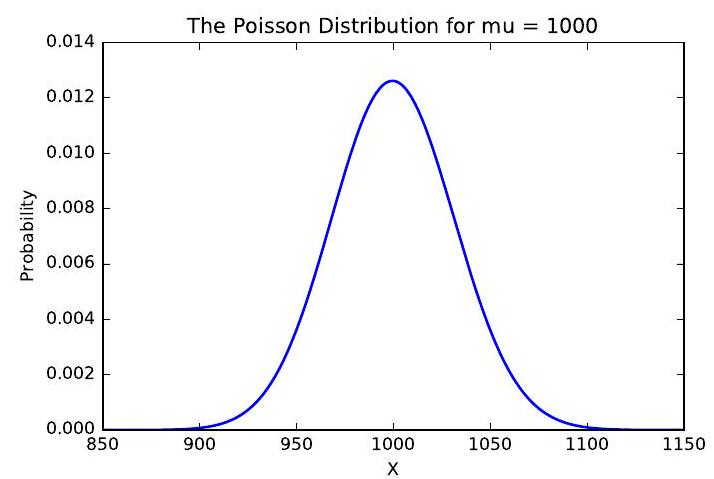
\includegraphics[max width=\textwidth]{2025_03_17_ca60ec0bfd96dcf8e028g-144}
\caption{The \textenglish{lifespan} \textenglish{distribution} \textenglish{of} \textenglish{lightbulbs} \textenglish{with} \textenglish{an} \textenglish{expected} \textenglish{life} \textenglish{of} $\mu=$ 1000 hours, \textenglish{as} \textenglish{modeled} \textenglish{by} \textenglish{a} \textenglish{Poisson} distribution.}
\label{fig:poisson-distribution}
\end{figure}

वैकल्पिक रूप से, मान लीजिए हम बच्चों की संख्या को एक प्रक्रिया द्वारा मॉडल करते हैं जहाँ परिवार बच्चों को तब तक पैदा करता रहता है जब तक कि एक के बाद एक बहुत सारे गुस्से के दौरे, बेक बिक्री, या कपड़े धोने के बाद, एक माता-पिता आखिरकार टूट जाते हैं। "बस बहुत हो गया! मैंने इसका काफी सामना कर लिया। अब और नहीं!"

ऐसे मॉडल के तहत, परिवार का आकार एक प्वासंद वितरण के रूप में मॉडल किया जाना चाहिए, जहां हर दिन एक छोटी लेकिन शून्य से भिन्न संभावना होती है कि एक टूट-फूट होगी जिसके परिणामस्वरूप फैक्टरी बंद हो जाएगी।

"मैंने बहुत सहन कर लिया" मॉडल परिवार के आकार की भविष्यवाणी करने में कितना प्रभावी है? चित्र\ref{fig:family-size}प्वाज़ॉन वितरण को $\lambda=2.2$ पैरामीटर के साथ दर्शाता है, जिसका अर्थ है कि परिवारों में औसतन 2.2 बच्चे होते हैं। बिंदु 2010 यू.एस. सामान्य सामाजिक सर्वेक्षण (\textenglish{GSS}) से लिए गए$k$बच्चों वाले परिवारों का अंश दर्शाते हैं।

\begin{figure}[h]
\centering
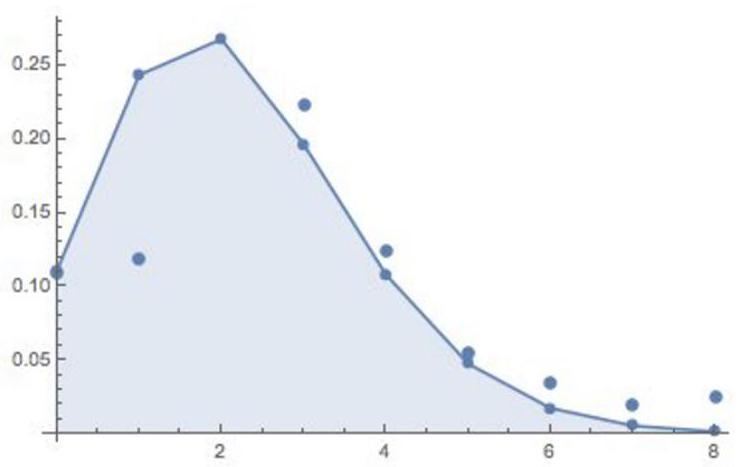
\includegraphics[max width=\textwidth]{2025_03_17_ca60ec0bfd96dcf8e028g-144(1)}
\caption{The \textenglish{observed} \textenglish{fraction} \textenglish{of} \textenglish{families} \textenglish{with} $x$ \textenglish{kids} (\textenglish{isolated} \textenglish{points}) \textenglish{is} \textenglish{accurately} \textenglish{modeled} \textenglish{by} \textenglish{Poisson} distribution, \textenglish{defined} \textenglish{by} \textenglish{an} \textenglish{average} \textenglish{of} $\mu=2.2$ \textenglish{children} \textenglish{per} \textenglish{family} (\textenglish{polyline}).}
\label{fig:family-size}
\end{figure}

सभी परिवार के आकारों पर उत्कृष्ट सहमति है, सिवाय $k=1$ के, और साफ़ तौर पर, मेरा व्यक्तिगत अनुभव सुझाव देता है कि इस डेटा सेट में दिखाई गई संख्या से अधिक अकेले बच्चे हैं। मिलकर, केवल औसत और पोइसन वितरण के लिए सूत्र को जानकर हम वास्तविक परिवार के आकार का एक उचित अनुमान बना सकते हैं।

% Mismatched: \sectionname{Power \textenglish{Law} Distributions}

कई डेटा वितरण सामान्य या पॉइसन वितरण के तहत जितना संभव हो, उससे कहीं लंबे पूंछ दर्शाते हैं। उदाहरण के लिए, शहरों की आबादी पर विचार करें। विकिपीडिया के अनुसार, 2014 में अमेरिका के 297 शहर थे जिनकी आबादी 100,000 लोगों से अधिक थी। $k$वें सबसे बड़े शहर की आबादी के लिए$1\leqk\leq297$, चित्र\ref{fig:city-populations} में प्रस्तुत की गई है। यह दिखाता है कि अपेक्षाकृत कम संख्या में शहरों की आबादी बाकी की तुलना में अत्यधिक प्रभावशाली है। वास्तव में, सबसे बड़े सत्रह शहरों की आबादी इतनी बड़ी है कि उन्हें इस प्लॉट से काट दिया गया है ताकि हम बाकी का देख सकें।

इन शहरों की औसत जनसंख्या 304,689 है, जिसमें 599,816 का भयानक मानक विचलन है। जब मानक विचलन औसत के मुकाबले इतना बड़ा होता है, तो कुछ गलत है। एक सामान्य वितरण के तहत,$99.7\%$मास औसत के$3\sigma$के भीतर स्थित होता है, इसलिए यह संभव नहीं है कि इन शहरों में से किसी की जनसंख्या 2.1 मिलियन लोगों से अधिक होगी। फिर भी ह्यूस्टन की जनसंख्या 2.2 मिलियन लोगों की है, और न्यूयॉर्क (8.4 मिलियन लोग) औसत से$13\sigma$से भी अधिक है! शहर की जनसंख्याएँ स्पष्ट रूप से सामान्य रूप से वितरित नहीं होतीं। वास्तव में, वे एक अलग वितरण का पालन करती हैं, जिसे पावर लॉ कहा जाता है।

\begin{figure}[h]
\centering
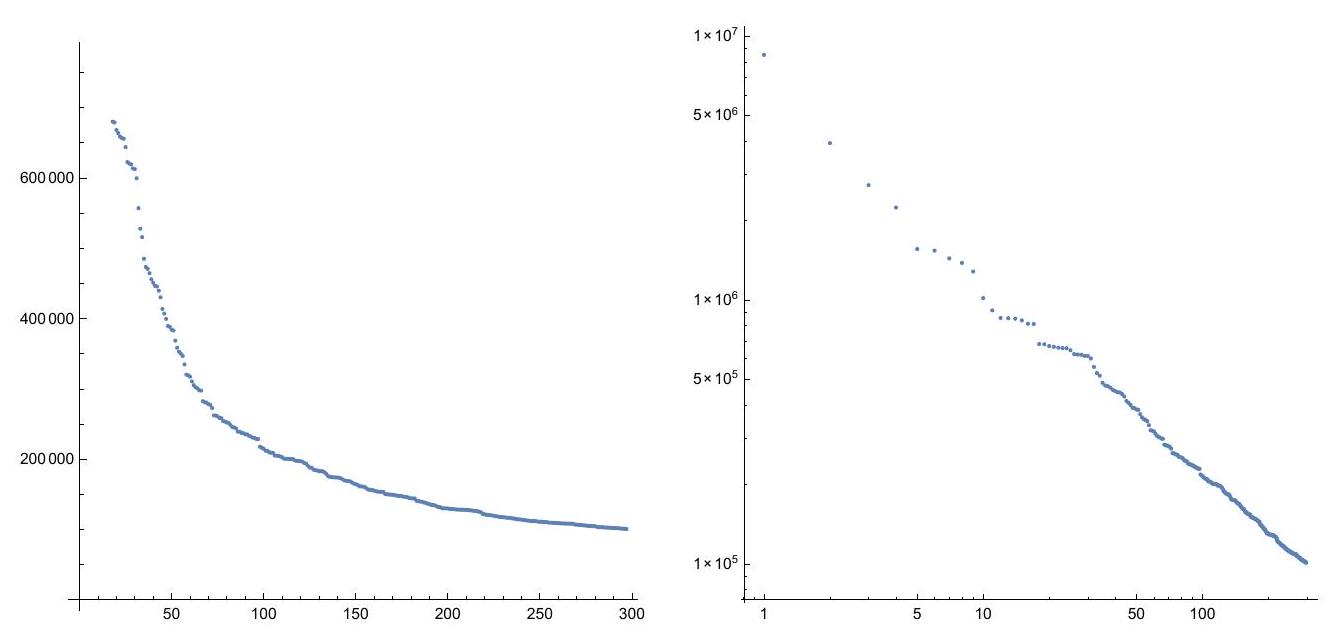
\includegraphics[max width=\textwidth]{2025_03_17_ca60ec0bfd96dcf8e028g-145}
\caption{The \textenglish{population} \textenglish{of} U.S. \textenglish{cities} \textenglish{by} \textenglish{decreasing} \textenglish{rank} (\textenglish{left}). \textenglish{On} \textenglish{the} \textenglish{right} \textenglish{is} \textenglish{the} \textenglish{same} data, \textenglish{now} \textenglish{including} \textenglish{the} \textenglish{very} \textenglish{largest} cities, \textenglish{but} \textenglish{plotted} \textenglish{on} \textenglish{a} log-log scale. \textenglish{That} \textenglish{they} \textenglish{sit} \textenglish{on} \textenglish{a} \textenglish{line} \textenglish{is} \textenglish{indicative} \textenglish{of} \textenglish{a} \textenglish{power} \textenglish{law} distribution.}
\label{fig:city-populations}
\end{figure}

दिए गए चर $X$ को एक पावर लॉ वितरण द्वारा परिभाषित किया गया है, 
\[
P(X=x)=cx^{-\alpha}
\]
यह दो स्थिरांकों द्वारा पैरामीटरित है: घातांक$\alpha$और सामान्यीकरण स्थिरांक $c$।

पावर लॉ वितरणों को सही ढंग से समझने के लिए कुछ सोचने की आवश्यकता होती है। इस वितरण द्वारा परिभाषित कुल प्रायिकता वक्र के नीचे का क्षेत्रफल होता है:
\[
A=\int_{x=-\infty}^{\infty}c x^{-\alpha}=c\int_{x=-\infty}^{\infty}x^{-\alpha}
\]

$A$ का विशेष मान$\alpha$ और $c$ के मानकों द्वारा परिभाषित किया गया है। सामान्यकरण स्थिरांक $c$ को विशेष रूप से एक दिए गए$\alpha$ के लिए चुना जाता है ताकि यह सुनिश्चित किया जा सके कि $A=1$, जैसा कि संभावना के नियमों द्वारा मांगा गया है। इसके अलावा, $c$ का कोई विशेष महत्व हमारे लिए नहीं है।\index{coefficient vector}\index{least \textenglish{squares} regression}\index{linear regression!solving}\index{matrix}\index{error!residual}\index{linear regression!error}

वास्तविक क्रिया $\alpha$ के साथ होती है। ध्यान दें कि जब हम प्रवेश इनपुट के मान को दोगुना करते हैं ( $x$ से $2x$ तक), हम संभावना को $f=2^{-\alpha}$ के घटक द्वारा कम कर देते हैं। यह बुरा लगता है, लेकिन किसी भी दिए गए $\alpha$ के लिए यह सिर्फ एक स्थिरांक है। तो जो शक्ति नियम वास्तव में कह रहा है, वह यह है कि $2x$-आकार की घटना की संभावना $x\alpha-आकार की घटना की तुलना में $2^{$}$ बार कम होती है, सभी $x$ के लिए।

व्यक्तिगत संपत्ति को पावर लॉ द्वारा अच्छी तरह से मॉडल किया गया है, जहाँ$f\approx0.2=1 / 5$। इसका अर्थ है कि एक बड़े दायरे में, यदि$Z$लोगों के पास$x$डॉलर हैं, तो$Z / 5$लोगों के पास$2x$डॉलर होंगे। एक पांचवें भाग के लोग\$200,000 के मुक़ाबले\$100,000 रखते हैं। यदि दुनिया में 625 लोगों की संपत्ति\$5 बिलियन है, तो लगभग 125 मल्टी-बिलिनियर्स होनी चाहिए, जिनमें से प्रत्येक की संपत्ति\$10 बिलियन है। आगे, 25 सुपरबिलिनियर्स होनी चाहिए, जिनमें से प्रत्येक की संपत्ति\$20 बिलियन है, पाँच हाइपर-बिलिनियर्स\$40 बिलियन स्तर पर, और अंततः एक अकेला बिल गेट्स\$80 बिलियन की संपत्ति वाला होना चाहिए।

पावर लॉ "80/20" नियमों को परिभाषित करते हैं जो हमारे विश्व की सभी असमानताओं का हिसाब रखते हैं: यह पर्यवेक्षण कि शीर्ष 20%⸨का$A$⸩ संपूर्ण 80% के ⸨का$B$⸩ पर नियंत्रण रखता है। पावर लॉ अक्सर उभरते हैं जब अमीर और अमीर बनते जाते हैं, जहाँ इस बात की बढ़ती संभावना होती है कि आपको और अधिक मिलेगा इस आधार पर कि आपके पास पहले से क्या है। बड़े शहर असमान रूप से बड़े हो जाते हैं क्योंकि बड़े शहरों में अधिक लोग आकर्षित होते हैं। अपनी संपत्ति की वजह से, बिल गेट्स को मुझसे कहीं बेहतर निवेश अवसर मिलते हैं, इसलिए उनका पैसा मेरे मुकाबले तेजी से बढ़ता है।

बहुत सी वितरणों को ऐसे प्राथमिकता वाले वृद्धि या अनुलग्न मॉडल्स द्वारा परिभाषित किया जाता है, जिनमें शामिल हैं:

\begin{itemize}
  \item इंटरनेट साइट्स जिनके $x$ उपयोगकर्ता हैं: वेबसाइटें अधिक लोकप्रिय हो जाती हैं क्योंकि उनके अधिक उपयोगकर्ता होते हैं। आप अधिक संभावना से \textenglish{Instagram} या \textenglish{Facebook} से जुड़ेंगे क्योंकि आपके मित्र पहले से \textenglish{Instagram} या \textenglish{Facebook} से जुड़ चुके हैं। प्रेफरेंशियल अटेचमेंट पावर लॉ वितरण की ओर ले जाता है।
  \item $x$ की तुलनात्मक आवृत्ति के साथ प्रयोग किए गए शब्द: \textit{algorist} या \textit{defenestrate}\footnote{Defenestrate का अर्थ है "किसी को खिड़की से बाहर फेंकना।"} जैसे लाखों शब्दों की एक लंबी श्रृंखला है जो अंग्रेजी भाषा में बहुत कम उपयोग होते हैं। दूसरी ओर, \textit{the} जैसे शब्दों का एक छोटा सेट है जो बाकी की तुलना में बहुत ज्यादा प्रयोग होते हैं।
\end{itemize}

ज़िप्फ़ का नियम प्राकृतिक भाषाओं में शब्द उपयोग के वितरण को नियंत्रित करता है और यह बताता है कि सबसे लोकप्रिय शब्द का$k$वां सबसे लोकप्रिय शब्द (आवृत्ति रैंक द्वारा मापा गया) सबसे लोकप्रिय शब्द के मुकाबले केवल$1/k$वां ही उपयोग किया जाता है। यह कितना अच्छा काम करता है, यह समझने के लिए, नीचे इंग्लिश विकिपीडिया से आवृत्तियों के आधार पर शब्दों की रैंक पर विचार करें:



\begin{tabular}{c|c|c}
\textenglish{Rank} & \textenglish{Word} & \textenglish{Count} \\
\hline
1017 & \textenglish{build} & 41890 \\
2017 & \textenglish{essential} & 21803 \\
3018 & \textenglish{sounds} & 13867 \\
4018 & \textenglish{boards} & 9811 \\
5018 & \textenglish{rage} & 7385 \\
6019 & \textenglish{occupied} & 5813 \\
7020 & \textenglish{continually} & 4650 \\
8020 & \textenglish{delay} & 3835 \\
9021 & \textenglish{delayed} & 3233 \\
10021 & \textenglish{glances} & 2767 \\
\end{tabular}

\begin{tabular}{c|c|c}
\textenglish{Rank} & \textenglish{Word} & \textenglish{Count} \\
\hline
10021 & \textenglish{glances} & 2767 \\
20026 & \textenglish{ecclesiastical} & 881 \\
30028 & zero-sum & 405 \\
40029 & \textenglish{excluded} & 218 \\
50030 & \textenglish{sympathizes} & 124 \\
60034 & \textenglish{capon} & 77 \\
70023 & \textenglish{fibs} & 49 \\
80039 & \textenglish{conventionalized} & 33 \\
90079 & \textenglish{grandmom} & 23 \\
100033 & slum-dwellers & 17 \\
\end{tabular}

\end{center}

यह विश्वासनीय होना चाहिए कि उपयोग की आवृत्ति जल्दी से रैंक के साथ कम हो जाती है: याद रखें कि\textit{ग्रैंडमॉम}केवल\textit{ग्रैंडमा}का एक स्लैंग रूप है, असली मैककॉय नहीं।

यह एक पावर लॉ क्यों है? एक शब्द जिसकी रैंक$2x$है, उसकी आवृत्ति $F_{2x}\simF_{1}/2x$ होती है, जबकि $F_{x}\simF_{1}/x$ के मुकाबले। इस प्रकार रैंक का आधा होना आवृत्ति को दोगुना कर देता है, और यह पावर लॉ से मेल खाता है जब$\alpha=1$।
भाषाओं के विकास के पीछे क्या तंत्र है जो इस वितरण की ओर ले जाता है? एक संभावित व्याख्या यह है कि लोग शब्दों को सीखते और उपयोग करते हैं क्योंकि वे अन्य लोगों को उनका उपयोग करते हुए सुनते हैं। किसी भी तंत्र जो पहले से लोकप्रिय शब्दों को समर्थन देता है, पावर लॉ की ओर ले जाता है।

\begin{itemize}
  \item भूकंप की आवृत्ति जिसका परिमाण $x$ है: भूकंप की तीव्रता मापने के लिए रिक्टर स्केल लघुगणकीय होती है, जिसका अर्थ है कि एक 5.3 की तीव्रता वाला भूकंप 4.3 पैमाने की घटना से दस गुना अधिक शक्तिशाली होता है। परिमाण में एक जोड़ने से शक्ति दस के गुणक से गुणा हो जाती है।\\\index{feature scaling}\index{target scaling}\index{non-linear classifiers!fitting}
इतनी तेजी से बढ़ते पैमाने के साथ समझ में आता है कि बड़े घटनाएँ छोटे घटनाओं की तुलना में दुर्लभ होती हैं। मैं हर बार जब शौचालय फ्लश करता हूं तो 0.02 परिमाण का भूकंप उत्पन्न करता हूं। सचमुच, हर दिन ऐसी अरबों घटनाएँ होती हैं, लेकिन आकार के साथ बड़े भूकंप दुर्लभ होते जाते हैं। जब भी कोई मात्रा संभावित रूप से असंयमित तरीके से बढ़ती है लेकिन इसकी संभावना घटती जाती है, तो आपको एक शक्ति विधि मिलती है। डेटा दिखाता है कि यह सच है जैसे भूकंपों द्वारा जारी ऊर्जा के लिए होता है, वैसे ही युद्धों के हताहतों के लिए भी: रहमदिल से, जिन संघर्षों में $x$ लोगों की मृत्यु होती है, संख्या शक्ति विधि के अनुसार घटती जाती है।
\end{itemize}

अपने आँखें खोलकर पावर लॉ वितरणों की तलाश करना सीखें। आप इन्हें हमारी अन्यायपूर्ण दुनिया में हर जगह पाएंगे। ये निम्नलिखित गुणों द्वारा प्रकट होते हैं:

\begin{itemize}
  \item पावर लॉग मूल्य, लॉग फ्रिक्वेंसी प्लॉट्स पर सीधी रेखाएं दिखाते हैं: \ref{fig:city-populations} चित्र में शहरों की जनसंख्या के ग्राफ को देखें। हालाँकि किनारों पर कुछ खाली स्थान हो सकते हैं जहाँ डेटा कम हो जाता है, फिर भी ज्यादातर बिंदु एक पंक्ति पर सुव्यवस्थित होते हैं। यह पावर लॉ की मुख्य विशेषता है। वैसे, इस रेखा की ढलान $\alpha$ द्वारा निर्धारित होती है, जो पावर लॉ वितरण के आकार को परिभाषित करने वाला स्थिरांक है।
  \item औसत का कोई अर्थ नहीं बनता: केवल बिल गेट्स के कारण संयुक्त राज्य अमेरिका में औसत व्यक्ति के धन में लगभग \$250 जुड़ जाते हैं। यह अजीब है। एक पावर लॉ वितरण के तहत, ऐसा बहुत ही कम लेकिन गैर-शून्य संभावना होती है कि किसी के पास असीमित धन होगा, तो इसका औसत पर क्या प्रभाव पड़ता है? माध्यिका ऐसे वितरणों के \textenglish{bulk} को पकड़ने का काम अधिक बेहतर ढंग से करती है बनिस्पत देखे गए औसत के।
  \item मानक विचलन का कोई अर्थ नहीं बनता: एक पावर लॉ वितरण में, मानक विचलन प्रायः औसत से उतना ही बड़ा या बड़ा होता है। इसका मतलब है कि वितरण को $\mu$ और $\sigma$ द्वारा बहुत खराब तरह से संचरित किया जाता है, जबकि पावर लॉ $\alpha$ और $c$ की दृष्टि से बहुत अच्छा विवरण प्रदान करता है।
  \item वितरण पैमाना-स्वतंत्र है: मान लीजिए कि हमने संयुक्त राज्य अमेरिका के 300वें से 600वें सबसे बड़े शहरों की जनसंख्या का रेखाचित्रण किया, शीर्ष 300 की बजाय जैसे \ref{fig:city-populations} चित्र में। आकार बहुत हद तक वैसा ही दिखाई देगा, जिसमें 300वें सबसे बड़े शहर की जनसंख्या पूंछ पर बहुत अधिक होती है। कोई भी घातीय फलन पैमाना-स्वतंत्र होता है, क्योंकि यह किसी भी समाधान पर समान दिखता है। यह लघु-लघु प्लॉट पर सीधी रेखा होने का परिणाम है: कोई भी उपरेंज सीधी रेखा खंड होता है, जिसके विंडो में वही पैरामीटर होते हैं जो कि पूर्ण वितरण में होते हैं।
\end{itemize}

\subsection{घर ले जाने वाला पाठ}
पावर लॉ वितरण के लिए सतर्क रहें। वे दुनिया की असमानताओं को दर्शाते हैं, जिसका अर्थ है कि वे हर जगह होते हैं।

\section{वितरणों से सैंपलिंग}
किसी दी गई प्रायिकता वितरण से बिंदुओं का सैंपल लेना एक सामान्य संचालन है, जिसे करना जानने में लाभ होता है। शायद आपको कोई सिमुलेशन चलाने के लिए पावर लॉ वितरण से परीक्षण डेटा की आवश्यकता हो, या यह सत्यापित करने के लिए कि आपका प्रोग्राम अत्यधिक स्थितियों में काम करता है। यह जाँच करने के लिए कि आपका डेटा वास्तव में किसी विशेष वितरण से मेल खाता है या नहीं, उसे किसी चीज़ के साथ तुलना करने की आवश्यकता होती है, और वह सामान्यतः सही रूप से उत्पन्न की गई सिंथेटिक डेटा होनी चाहिए जो आदर्श वितरण से खींची गई हो।\index{power \textenglish{law} function}\index{target scaling!sublinear}

किसी भी दिए गए प्रायिकता वितरण से सैंपलिंग के लिए एक सामान्य तकनीक होती है, जिसे\textit{विपरीत परिवर्तन सैंपलिंग}कहा जाता है। याद करें कि हम प्रायिकता घनत्व फलन$P$और संचयी घनत्व फलन$C$के बीच समाकलन और अवकलन द्वारा चल सकते हैं। हम इनके बीच आगे और पीछे चल सकते हैं क्योंकि:\index{dimension reduction}\index{feature scaling!highly-correlated}\index{New York}\index{target scaling!tipping rate}\index{taxi driver}

\[
P(k=X)=C^{\prime}(\textenglish{k})=C(\textenglish{X} \leq k+\delta)-C(\textenglish{X} \leq \textenglish{k}), \text{ \textenglish{and} }
\]

\[
C(\textenglish{X} \leq \textenglish{k})=\int_{x=-\infty}^{k} P(X=x)
\]

\begin{figure}[h]
\centering
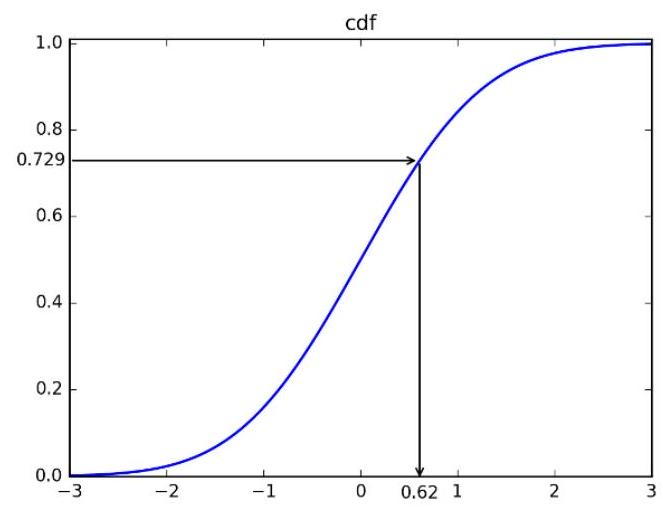
\includegraphics[max width=\textwidth]{2025_03_17_ca60ec0bfd96dcf8e028g-149}
\caption{The \textenglish{inverse} \textenglish{transform} \textenglish{sampling} \textenglish{method} \textenglish{enables} \textenglish{us} \textenglish{to} \textenglish{convert} \textenglish{a} \textenglish{random} \textenglish{number} \textenglish{generated} \textenglish{uniformly} \textenglish{from} [0,1] (\textenglish{here} 0.729) \textenglish{to} \textenglish{a} \textenglish{random} \textenglish{sample} \textenglish{drawn} \textenglish{from} \textenglish{any} distribution, \textenglish{given} \textenglish{its} cdf.}
\label{fig:inverse-transform}
\end{figure}

मान लें कि मैं इस संभवतः बहुत जटिल वितरण से एक बिंदु को नमूना लेना चाहता हूँ। मैं एक समान यादृच्छिक संख्या जनरेटर का उपयोग कर सकता हूँ ताकि $p$ मान को अंतराल $[0,\ldots, 1]$ में चुना जा सके। हम $p$ को एक प्रायिकता के रूप में व्याख्या कर सकते हैं, और इसे संचयी वितरण $C$ पर एक सूचकांक के रूप में उपयोग कर सकते हैं। विशेष रूप से, हम $x$ के उस सटीक मान की रिपोर्ट करते हैं ताकि $C(X\leqx)=p$।

चित्र\ref{fig:inverse-transform}इस दृष्टिकोण को दर्शाता है, यहाँ सामान्य वितरण से नमूना लिया जाता है। मान लीजिए$p=0.729$हमारे यूनिफॉर्म जनरेटर से चयनित यादृच्छिक संख्या है। हम वह$x$मान लौटाते हैं ताकि$y=0.729$, यहाँ$x=0.62$इस \textenglish{cdf} के अनुसार है।

यदि आप पायथन जैसी अच्छी तरह से समर्थित भाषा में किसी लोकप्रिय संभावना वितरण के साथ काम कर रहे हैं, तो लगभग निश्चित रूप से एक पुस्तकालय फंक्शन पहले से ही उपलब्ध होता है जो यादृच्छिक नमूने उत्पन्न करता है। इसलिए, अपनी खुद की लिखने से पहले सही पुस्तकालय की तलाश करें।

\subsection{एक आयाम से परे यादृच्छिक नमूना}
किसी दिए गए वितरण से सही ढंग से नमूना लेने का कार्य बहुत ही जटिल हो जाता है जब आप आयामों की संख्या बढ़ाते हैं। एक वृत्त के भीतर से बिंदुओं को समान रूप से नमूना लेने का कार्य सोचें। इससे पहले कि हम आगे बढ़ें, एक पल के लिए सोचें कि आप इसे कैसे कर सकते हैं।

%---- \textenglish{Page} \textenglish{End} \textenglish{Break} \textenglish{Here} ---- \textenglish{Page} : 133

\begin{figure}[H]
    \centering
    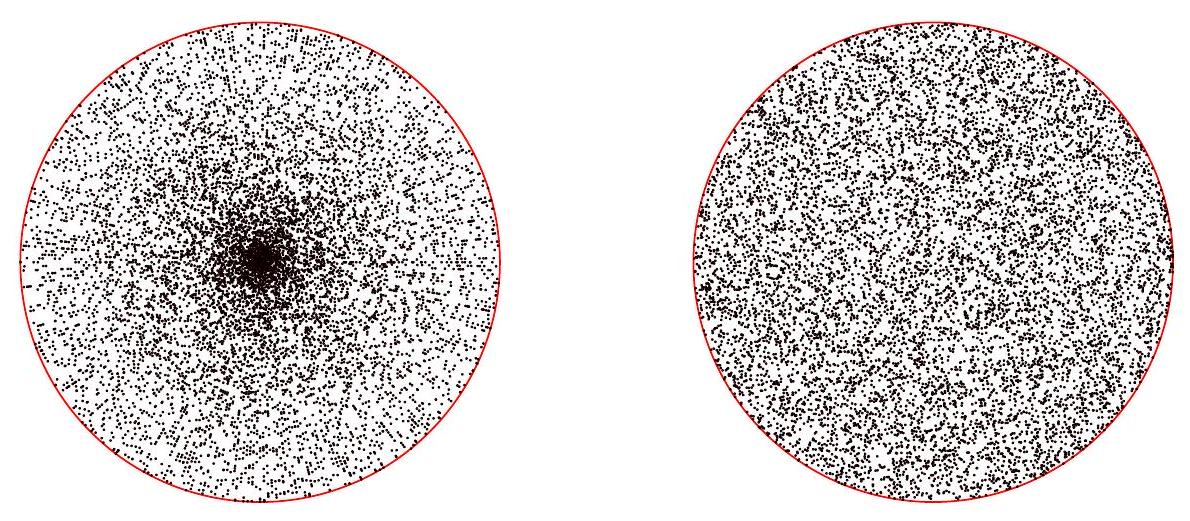
\includegraphics[max width=\textwidth]{2025_03_17_ca60ec0bfd96dcf8e028g-150}
    \caption{Randomly \textenglish{generating} 10,000 \textenglish{points} \textenglish{by} angle-radius \textenglish{pairs} \textenglish{clearly} \textenglish{oversamples} \textenglish{near} \textenglish{the} \textenglish{origin} \textenglish{of} \textenglish{the} \textenglish{circle} (\textenglish{left}). \textenglish{In} contrast, \textenglish{Monte} \textenglish{Carlo} \textenglish{sampling} \textenglish{generates} \textenglish{points} \textenglish{uniformly} \textenglish{within} \textenglish{the} \textenglish{circle} (\textenglish{right}).}
    \label{fig:random_points}
\end{figure}

आप में से जो चालाक हैं, वे केंद्र से कोण और दूरी को स्वतंत्र रूप से नमूना लेने का विचार कर सकते हैं। किसी भी नमूनित बिंदु को उद्गम और सकारात्मक $x$-अक्ष के संबंध में जो कोण बनाना चाहिए वह $0$ और $2\pi$ के बीच बदलता है। उद्गम से दूरी $0$ और $r$ के बीच का एक मान होना चाहिए। इन निर्देशांक का समान रूप से यादृच्छिक चयन करें और आपके पास वृत्त में एक यादृच्छिक बिंदु होगा।

यह विधि चतुराईपूर्ण है, लेकिन गलत है। निश्चित रूप से, इस प्रकार बनाये गए कोई भी बिंदु वृत्त के भीतर ही होंगे। लेकिन बिंदु समान आवृत्ति के साथ नहीं चुने जाते हैं। यह विधि ऐसे बिंदु उत्पन्न करेगी जहाँ उनका आधा भाग केंद्र से अधिकतम$r / 2$की दूरी के भीतर होगा। लेकिन वृत्त का अधिकांश क्षेत्र केंद्र से दूर ही होता है! इस प्रकार हम मूल के समीप अधिक बिंदु चुनेंगे, और किनारे के समीप की मात्रा को नजरअंदाज करेंगे। यह\ref{चित्र~fig:random_points}(बाएँ) में दिखाया गया है, जो इस विधि का उपयोग करके उत्पन्न 10,000 बिंदुओं का ग्राफ है।\index{parameter fitting}

एक साधारण तकनीक जो सही साबित होती है, वह है \textit{मोंटे कार्लो सैंपलिंग}। $x$ और $y$ निर्देशांक का हर बिंदु वृत्त में $-r$ से $r$ तक होता है, जैसे कि वृत्त के बाहर कई बिंदु। इस प्रकार इन मूल्यों को यादृच्छिक रूप से समान रूप से नमूना लेने से हमें एक बिंदु मिलता है जो वृत्त के बाउंडिंग बॉक्स में स्थित होता है, लेकिन हमेशा वृत्त के भीतर नहीं होता। इसे आसानी से जांचा जा सकता है: क्या $(x, \textenglish{y})$ से मूल तक की दूरी अधिकतम $r$ है, यानी क्या $\sqrt{x^{2}+y^{2}}\leqr$ है? अगर हाँ, तो हमने वृत्त में एक यादृच्छिक बिंदु पाया है। अगर नहीं, तो हम इसे छोड़कर फिर से प्रयास करते हैं। आकृति~\ref{fig:random_points}(दाईं ओर) इस विधि का उपयोग करके 10,000 बिंदु प्रदर्शित करती है: देखें कि वे सरलता से वृत्त को कैसे आवृत करते हैं, बिना किसी स्थान के अधिक या कम नमूनाकरण के।

यहाँ दक्षता पूरी तरह से वांछित क्षेत्र की मात्रा (वृत्त का क्षेत्रफल) और बाउंडिंग बॉक्स की मात्रा (वर्ग का क्षेत्रफल) के अनुपात पर निर्भर करती है। चूँकि इस बाउंडिंग बॉक्स का 78.5% भाग वृत्त द्वारा कब्जा किया गया है, औसतन दो से कम प्रयास प्रत्येक नए वृत्त बिन्दु को खोजने के लिए पर्याप्त होते हैं।

\begin{figure}[H]
    \centering
    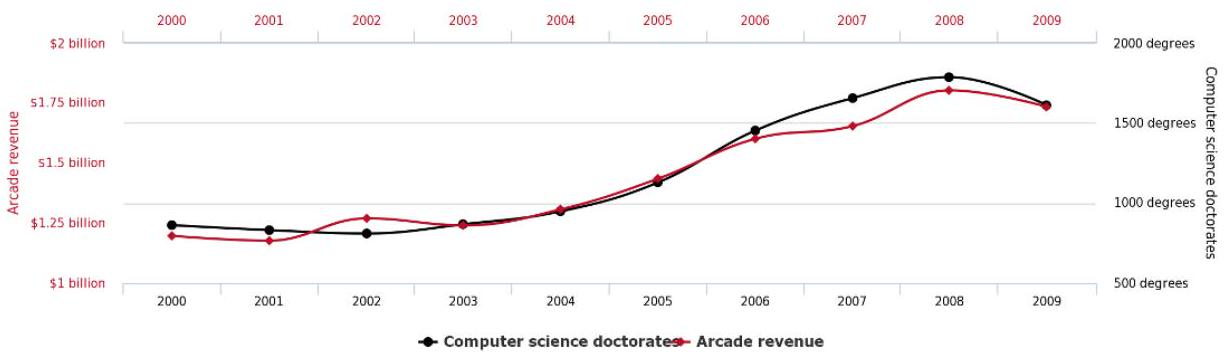
\includegraphics[max width=\textwidth]{2025_03_17_ca60ec0bfd96dcf8e028g-151}
    \caption{Correlation vs. causation: \textenglish{the} \textenglish{number} \textenglish{of} \textenglish{Computer} \textenglish{Science} Ph.Ds \textenglish{awarded} \textenglish{each} \textenglish{year} \textenglish{in} \textenglish{the} \textenglish{United} \textenglish{States} \textenglish{strongly} \textenglish{correlates} \textenglish{with} video/pinball \textenglish{arcade} revenue. (\textenglish{from} \cite{vigen2015spurious})}
    \label{fig:correlation_vs_causation}
\end{figure}

\section{सांख्यिकीय महत्व}
सांख्यिकीविद मुख्य रूप से चिंतित होते हैं कि डेटा पर अवलोकन महत्वपूर्ण हैं या नहीं। संगणकीय विश्लेषण किसी भी दिलचस्प डेटा सेट में आसानी से कई पैटर्न और संबंध खोज लेगा। लेकिन क्या विशिष्ट संबंध वास्तव में किसी वास्तविक घटना को दर्शाते हैं, मात्र संयोग के विपरीत? दूसरे शब्दों में, एक अवलोकन \textit{वास्तव में महत्वपूर्ण} कब होता है?

बड़े डेटा सेट पर पर्याप्त रूप से मजबूत सहसंबंध "स्पष्ट रूप से" महत्वपूर्ण लग सकते हैं, लेकिन मुद्दे अक्सर काफी जटिल होते हैं। एक बात के लिए, \textit{सहसंबंध का अर्थ कारण नहीं होता है}। आकृति~\ref{fig:correlation_vs_causation}प्रत्येक रूप से दर्शाती है कि कंप्यूटर विज्ञान में उन्नत अध्ययन की मात्रा का सहसंबंध वीडियो गेम खेलने की मात्रा से है। मैं सोचना चाहूंगा कि मैंने एल्गोरिदम की ओर निनटेंडो से अधिक लोगों को प्रेरित किया है, लेकिन शायद यह केवल वही चीज़ है? ऐसे झूठे सहसंबंधों के ग्राफ सचमुच एक पुस्तक में भरे हुए हैं \cite{vigen2015spurious}, और वह भी एक बहुत ही मजेदार।

सांख्यिकी का अनुशासन यह निर्धारित करने में सूक्ष्म भेद करता है कि क्या कोई अवलोकन सार्थक है या नहीं। चिकित्सा सांख्यिकी से एक क्लासिकल उदाहरण आता है, जब दवा उपचारों की प्रभावकारिता का निर्धारण किया जाता है। एक फ़ार्मास्युटिकल कंपनी दो दवाओं की तुलना में एक प्रयोग करती है। ड्रग$A$ ने 34 में से 19 मरीजों को ठीक किया। ड्रग$B$ ने 21 में से 14 मरीजों को ठीक किया। क्या ड्रग$B$ वास्तव में ड्रग$A$ से बेहतर है? नई दवाओं की \textenglish{FDA} स्वीकृति दवा कंपनियों के मूल्य में अरबों को जोड़ या घटा सकती है। लेकिन क्या आप सुनिश्चित हो सकते हैं कि कोई नई दवा वास्तव में सुधार दर्शाती है? आप यह कैसे तय करते हैं?

\subsection{महत्त्व के महत्त्व}
सांख्यिकीय महत्त्व हमें यह विश्वास दिलाता है कि दो दी गई वितरणों के बीच वास्तव में कोई अंतर है। यह महत्वपूर्ण है। लेकिन सांख्यिकीय महत्त्व इस अंतर के महत्व या परिमाण को नहीं मापता। बड़े\\index{derivative}\index{derivative!second}\index{gradient \textenglish{descent} search}\index{derivative!partial}\index{tangent line}

%---- \textenglish{Page} \textenglish{End} \textenglish{Break} \textenglish{Here} ---- \textenglish{Page} : 135

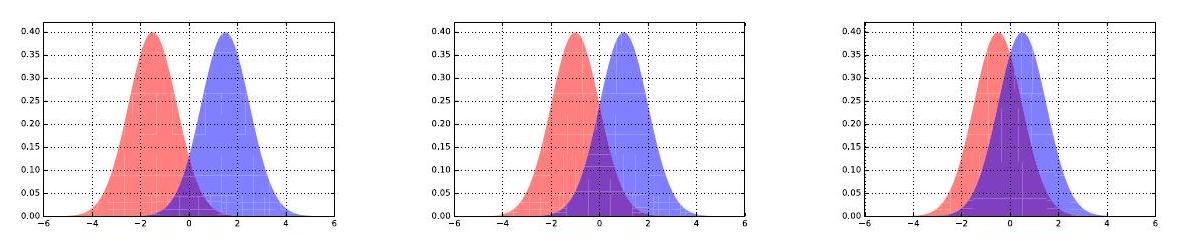
\includegraphics[max width=\textwidth, center]{2025_03_17_ca60ec0bfd96dcf8e028g-152}

\begin{figure}[H]
\centering
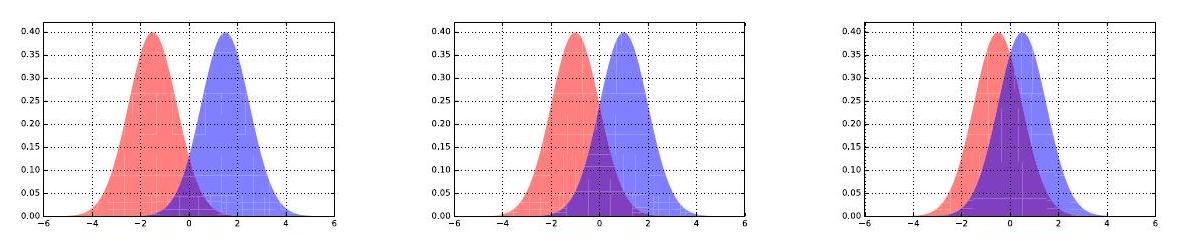
\includegraphics[max width=\textwidth]{2025_03_17_ca60ec0bfd96dcf8e028g-152}
\caption{Pairs \textenglish{of} \textenglish{normal} \textenglish{distributions} \textenglish{with} \textenglish{the} \textenglish{same} variance, \textenglish{but} \textenglish{decreasing} \textenglish{difference} \textenglish{in} \textenglish{their} \textenglish{means} \textenglish{from} \textenglish{left} \textenglish{to} right. \textenglish{As} \textenglish{the} \textenglish{means} \textenglish{get} closer, \textenglish{the} \textenglish{greater} \textenglish{overlap} \textenglish{between} \textenglish{the} \textenglish{distributions} \textenglish{makes} \textenglish{it} \textenglish{harder} \textenglish{to} \textenglish{tell} \textenglish{them} apart.}
\end{figure}

पर्याप्त नमूना आकार के साथ, अत्यंत छोटे अंतर सांख्यिकीय परीक्षणों पर अत्यधिक महत्वपूर्ण के रूप में दर्ज हो सकते हैं।

उदाहरण के लिए, मान लीजिए कि मुझे सिक्के के पीछे की शर्त लगाने के लिए फँसा दिया जाता है जो 51% बार चेहरे के रूप में आता है, बजाए इसके कि हम 50% के साथ निष्पक्ष सिक्के के साथ सोचते हैं। 100 बार निष्पक्ष सिक्के के उछाल के बाद, मैं 51% या उससे अधिक चेहरे देखने की उम्मीद करूंगा 46.02% बार, इसलिए मेरे पास कोई शिकायत के आधार नहीं हैं जब ऐसा होता है। 1,000 बार उछाल के बाद, कम से कम 510 चेहरे देखने की संभावना 0.274 पर गिर जाती है। 10,000 बार उछाल के बाद, इतने सारे चेहरे देखने की संभावना केवल 0.0233 है, और मुझे शक करना शुरू कर देना चाहिए कि क्या सिक्का निष्पक्ष है। 100,000 बार उछाल के बाद, निष्पक्षता की संभावना$1.29\times10^{-10}$ तक कम हो जाएगी, इतनी छोटी कि मुझे औपचारिक शिकायत दर्ज करनी पड़ेगी, भले ही मैंने अपने प्रतिद्वंद्वी को सज्जन समझा हो।

पर यहाँ बात यह है। हालांकि अब यह बिल्कुल स्पष्ट है कि मुझे पक्षपाती सिक्का इस्तेमाल करने के लिए धोखा दिया गया था, इस कार्य के परिणाम गंभीर नहीं हैं। जीवन के लगभग किसी भी महत्वपूर्ण मुद्दे के लिए, मैं सिक्के के छोटे हिस्से को लेने के लिए तैयार रहूँगा, क्योंकि दाँव बस इतना ऊँचा नहीं है। 1$ दाँव प्रति पलटने पर, मेरा अपेक्षित नुकसान 100,000 बार पलटने के बाद भी केवल 1$,000 रुपये होगा।

महत्त्व यह बताता है कि कुछ घटना संयोगवश होने की संभावना कितनी कम है, लेकिन यह नहीं बताता कि वह महत्वपूर्ण है या नहीं। हम वास्तव में\textit{प्रभाव आकार}के बारे में चिंतित रहते हैं, जो दो समूहों के बीच अंतर की मात्रा है। हम अनौपचारिक रूप से\textit{मध्यम}-स्तर के प्रभाव आकार को एक सतर्क पर्यवेक्षक द्वारा नग्न आँखों से दिखाई देने वाला श्रेणीबद्ध करते हैं। इस पैमाने पर,\textit{बड़े}प्रभाव स्पष्ट तौर पर सामने आते हैं, और\textit{छोटे}प्रभाव पूरी तरह से तुच्छ नहीं होते ⸨ हैं। कई सांख्यिकी मौजूद हैं जो प्रभाव आकार का मापने का प्रयास करते हैं, जिनमें शामिल हैं: ⸩⸨⸨⸨

\begin{itemize}
  \item \textit{कोहेन का} $d$: दो माध्यों के बीच के अंतर के महत्व $\mu$ और $\mu^{\prime}$ का निर्भर करता है परिवर्तन की पूर्ण सीमा पर, लेकिन यह भी वितरणों के प्राकृतिक परिवर्तन पर मापा गया $\sigma$ या $\sigma^{\prime}$ द्वारा। इस प्रभाव आकार को मापा जा सकता है:
\end{itemize}

\[
d=\frac{\left|\mu-\mu^{\prime}\right|}{\sigma}
\]

एक उचित सीमाप्रगति छोटे प्रभाव आकार के लिए है$>0.2$, मध्यम प्रभाव$>0.5$, और बड़ा प्रभाव आकार$>0.8$।

\begin{itemize}
\item\textit{पियर्सन का सहसंबंध गुणांक} $r$: दो चर के बीच रैखिक संबंध की डिग्री को मापता है, एक -1 से 1 तक के पैमाने पर। प्रभाव आकारों के लिए सीमा मूल्य औसत परिवर्तन के समान हैं: छोटे प्रभाव $\pm0.2$,
से शुरू होते हैं\end{itemize}

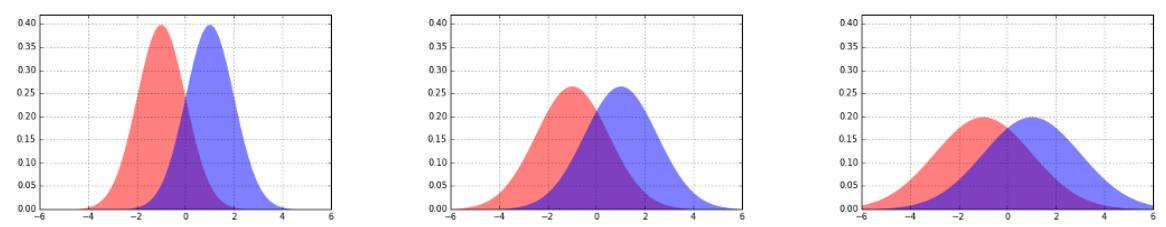
\includegraphics[max width=\textwidth, center]{2025_03_17_ca60ec0bfd96dcf8e028g-153}

\begin{figure}[H]
\centering
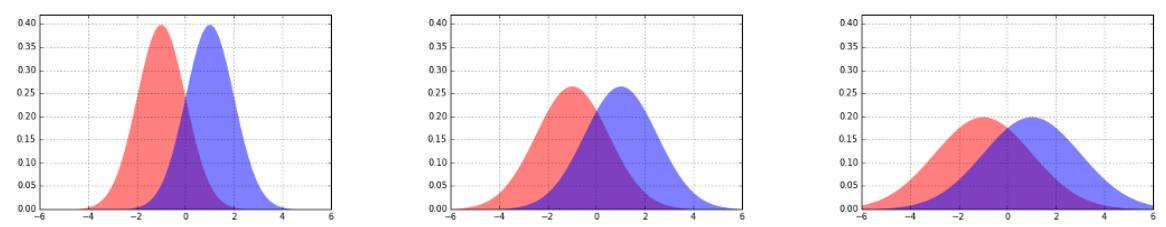
\includegraphics[max width=\textwidth]{2025_03_17_ca60ec0bfd96dcf8e028g-153}
\caption{Pairs \textenglish{of} \textenglish{normal} \textenglish{distributions} \textenglish{with} \textenglish{the} \textenglish{same} \textenglish{difference} \textenglish{in} \textenglish{their} \textenglish{means} \textenglish{but} \textenglish{increasing} variance, \textenglish{from} \textenglish{left} \textenglish{to} right. \textenglish{As} \textenglish{the} \textenglish{variance} increases, \textenglish{there} \textenglish{becomes} \textenglish{greater} \textenglish{overlap} \textenglish{between} \textenglish{the} distributions, \textenglish{making} \textenglish{it} \textenglish{harder} \textenglish{to} \textenglish{tell} \textenglish{them} apart.}
\end{figure}

मध्यम प्रभावों के बारे में$\pm0.5$, और बड़े प्रभाव आकारों के लिए सहसंबंधों के$\pm0.8$की आवश्यकता होती है।

\begin{itemize}
  \item \textit{भिन्नता की गुणांक} $r^{2}$: सहसंबंध गुणांक का वर्ग उस विचरण के अनुपात को दर्शाता है जो एक चर में दूसरे द्वारा समझाया गया है। ऊपर दिए गए वर्ग के उपयोग से ये सीमाएँ तय होती हैं। छोटे प्रभाव कम से कम 4\% विचरण को समझाते हैं, मध्यम प्रभाव $\geq 25\%$ और बड़े प्रभाव आकार कम से कम 64\%।
  \item \textit{अतिक्रमण का प्रतिशत}: किसी भी एकल प्रायिकता वितरण के तहत क्षेत्र, परिभाषा के अनुसार, 1 होता है। किसी दिए गए दो वितरणों के बीच प्रतिच्छेदन का क्षेत्र उनके समानता का एक अच्छा माप है, जैसा कि चित्र 5.11 में दिखाया गया है। समान वितरण 100\% ओवरलैप होते हैं, जबकि असमान अंतराल 0\% ओवरलैप होते हैं। तर्कसंगत सीमाएँ हैं: छोटे प्रभावों के लिए 53\% ओवरलैप, मध्यम प्रभावों के लिए 67\% ओवरलैप, और बड़े प्रभाव आकारों के लिए 85\% ओवरलैप।\index{modeling!simplifying}\index{Occam’s razor}\index{regression!ridge}\index{regularization}\index{target scaling!tipping model}
\end{itemize}

बेशक, कोई भी बड़ा प्रभाव जो सांख्यिकीय रूप से महत्वपूर्ण नहीं है, स्वाभाविक रूप से संदिग्ध होता है। चित्र 5.10 में सीएस अध्ययन बनाम वीडियो गेम खेलने के सहसम्बंध इतने अधिक थे ($r=0.985$) कि प्रभाव का आकार बहुत बड़ा होता, अगर नमूना बिंदुओं की संख्या और कार्यप्रणाली निष्कर्षों का समर्थन करने के लिए पर्याप्त होती।

\textit{घर ले जाने का सबक}: सांख्यिकीय महत्वपूर्णता नमूनों की संख्या पर निर्भर करती है, जबकि प्रभाव आकार नहीं करता।

% Mismatched: \sectionname{The T-test: \textenglish{Comparing} \textenglish{Population} Means}
\index{T-test}We \textenglish{have} \textenglish{seen} \textenglish{that} \textenglish{large} \textenglish{mean} \textenglish{shifts} \textenglish{between} \textenglish{two} \textenglish{populations} \textenglish{suggest} \textenglish{large} \textenglish{effect} sizes. \textenglish{But} \textenglish{how} \textenglish{many} \textenglish{measurements} \textenglish{do} \textenglish{we} \textenglish{need} \textenglish{before} \textenglish{we} \textenglish{can} \textenglish{safely} \textenglish{believe} \textenglish{that} \textenglish{the} \textenglish{phenomenon} \textenglish{is} real. \textenglish{Suppose} \textenglish{we} \textenglish{measure} \textenglish{the} \textenglish{IQs} \textenglish{of} \textenglish{twenty} \textenglish{men} \textenglish{and} \textenglish{twenty} women. \textenglish{Does} \textenglish{the} \textenglish{data} \textenglish{show} \textenglish{that} \textenglish{one} \textenglish{group} \textenglish{is} smarter, \textenglish{on} average? Certainly, \textenglish{the} \textenglish{sample} \textenglish{means} \textenglish{will} differ, \textenglish{at} \textenglish{least} \textenglish{a} bit, \textenglish{but} \textenglish{is} \textenglish{this} \textenglish{difference} significant?

t-टेस्ट इस बात का मूल्यांकन करता है कि दो नमूनों की जनसंख्या का औसत अलग है या नहीं। यह समस्या अक्सर \textit{एबी टेस्टिंग} में उठती है,\index{AB testing} जो मूल्यांकन से जुड़ी होती है।

%---- \textenglish{Page} \textenglish{End} \textenglish{Break} \textenglish{Here} ---- \textenglish{Page} : 137

% Mismatched: \sectionname{Statistical Analysis}

% Mismatched: \subsectionname{Statistical Significance}

उत्पाद में बदलाव प्रदर्शन में कोई परिवर्तन करता है या नहीं। मान लीजिए आप एक समूह को संस्करण \textenglish{A} दिखाते हैं, और दूसरे समूह को संस्करण B। इसके अलावा, मान लीजिए कि आप प्रत्येक उपयोगकर्ता के लिए सिस्टम प्रदर्शन मान मापते हैं, जैसे कि वे कितनी बार विज्ञापनों पर क्लिक करते हैं या जब उनसे अनुभव के बारे में पूछा जाता है तो वे इसे कितने स्टार देते हैं। टी-परीक्षण यह मापता है कि क्या दोनों समूहों के बीच देखी गई अंतर महत्वपूर्ण है।

दो माध्य महत्वपूर्ण रूप से भिन्न होते हैं यदि:

\begin{itemize}
\item \textit{औसत अंतर अपेक्षाकृत बड़ा है:} यह समझ में आता है। कोई व्यक्ति निष्कर्ष निकाल सकता है कि औसतन पुरुष महिलाओं से अधिक वजन रखते हैं, क्योंकि प्रभाव का आकार बहुत बड़ा है। रोग नियंत्रण केंद्र\footnote{\href{http://www.cdc.gov/nchs/fastats/obesity-overweight.htm}{http://www.cdc.gov/nchs/fastats/obesity-overweight.htm}} के अनुसार, 2010 में औसत अमेरिकी पुरुष का वजन 195.5 पाउंड था, जबकि औसत अमेरिकी महिला का वजन 166.2 पाउंड था। यह बड़ा अंतर है। जैसे आईक्यू का मामला, जो बहुत अधिक सूक्ष्म अंतर होता है, उसके वास्तविक होने को साबित करने के लिए कहीं अधिक प्रमाण की आवश्यकता होती है।
\item \textit{मानक विचलन पर्याप्त रूप से छोटे हैं:} यह भी समझ में आता है। यह खुद को समझाना आसान है कि औसतन पुरुषों और महिलाओं के पास उँगलियों की समान संख्या है क्योंकि जो गणना हम देखते हैं, वह औसत के आसपास बहुत ही सटीक जुड़ा हुआ है: \(\{10,10,10,10,9,10,\ldots\}\)। सम-उँगलियों की संख्या के परिकल्पना के लिए अधिक प्रमाण की आवश्यकता होगी अगर संख्याएँ अधिक इधर-उधर होतीं। मुझे एक सच्चे वितरणात्मक औसत \(\mu=10\) के लिए प्रतिबद्ध होने में संकोच होगा अगर जो मैंने देखा वह \(\{3,15,6,14,17,5\}\) था।\index{fit \textenglish{and} complexity}
\item \textit{नमूनों की संख्या पर्याप्त रूप से बड़ी है:} यह फिर समझ में आता है। जितना अधिक डेटा मैं देखता हूँ, उतना ही अधिक मैं इस बात से विश्वास में हो जाता हूँ कि नमूना अपनी अन्तर्निहित वितरण को सही ढंग से प्रस्तुत करेगा। उदाहरण के लिए, औसतन पुरुषों के पास महिलाओं की तुलना में \textit{कम} उँगलियाँ होती हैं क्योंकि वे पावर टूल्स के साथ अधिक साहसी होते हैं।\footnote{यह अवलोकन अकेले ही लिंग-आईक्यू संबंध को हल करने के लिए पर्याप्त हो सकता है, बिना अतिरिक्त सांख्यिकी प्रमाण की आवश्यकता के।} लेकिन इस अपेक्षाकृत दुर्लभ घटना का अवलोकन और पुष्टि करने के लिए बहुत बड़ी संख्या में नमूनों की आवश्यकता होगी।
\end{itemize}

t-परीक्षण दो अवलोकनों के समूहों पर एक परीक्षण सांख्यिक को गणना करके शुरू होता है। वेल्च का t-सांख्यिक इस प्रकार परिभाषित है

\begin{equation}
t=\frac{\bar{x}_{1}-\bar{x}_{2}}{\sqrt{\frac{\sigma_{1}^2}{n_{1}}+\frac{\sigma_{2}^2}{n_{2}}}}
\end{equation}

जहां\(\bar{x}_{i}\),\(\sigma_{i}\), और\(n_{i}\), नमूना\(i\) के औसत, मानक विचलन, और जनसंख्या आकार हैं, क्रमशः।

आइए इस समीकरण का ध्यानपूर्वक विश्लेषण करें। गुणांक के ऊपरी भाग में औसत का अंतर है, तो जितना बड़ा यह अंतर होगा, t-statistic का मान उतना ही बड़ा होगा। मानक विचलन हर के भाग में होते हैं, तो जितना छोटा वह\(\sigma_{i}\)होगा, t-statistic का मान उतना ही बड़ा होगा। यदि यह भ्रमित कर रहा है, तो याद करें कि जब आप\(x\)को शून्य की ओर बढ़ने वाली संख्या से विभाजित करते हैं तो क्या होता है। नमूना आकार\(n_{i}\)को बढ़ाना भी हर को छोटा बनाता है, तो जितना बड़ा\(n_{i}\)होगा, t-statistic का मान उतना ही बड़ा होगा। सभी मामलों में, वे घटक जो हमें दो वितरणों के बीच वास्तविक अंतर होने में अधिक आश्वस्त करते हैं, t-statistic के मान को बढ़ाते हैं।

किसी विशेष t-सांख्यिकी के मूल्य का अर्थ समझने के लिए उपयुक्त सारणी में एक संख्या देखना होता है। एक वांछित\textit{महत्व स्तर}\(\alpha\)और \textit{स्वतंत्रता की डिग्रियों}(मुख्यतः नमूना आकारों) की संख्या के लिए, सारणी की प्रविष्टि उस मूल्य\(v\)को निर्दिष्ट करती है जिसे t-सांख्यिकी\(t\)को पार करना चाहिए। यदि\(t>v\), तो अवलोकन \(\alpha\)स्तर के लिए महत्वपूर्ण होता है।

\subsection{यह कार्य क्यों करता है?}

आँकड़ों के परीक्षण जैसे t-परीक्षण अक्सर मेरे लिए जादू-टोना जैसे लगते हैं, क्योंकि हम किसी जादुई तालिका से एक संख्या देखते हैं और इसे महत्त्वपूर्ण मान लेते हैं। \textit{ओरेकल ने कहा है: अंतर महत्वपूर्ण है!} बेशक, महत्त्व परीक्षण के पीछे वास्तविक गणित है, लेकिन इसका निष्कर्षण कैलकुलस और अजीब फ़ंक्शन (जैसे गामा फ़ंक्शन \(\Gamma(\textenglish{n})\), जो फैक्टरियल्स का वास्तविक संख्या वाला सामान्यीकरण है) शामिल करता है। ये जटिल गणनाएँ ही कारण हैं कि प्री-कंप्यूटेड तालिका में चीज़ें देखने की प्रथा उभरी, स्वयं गणना करने के बजाय।

आप किसी भी अच्छे सांख्यिकी किताब में संबंधित सूत्रों की व्युत्पत्ति पा सकते हैं, यदि आप रुचि रखते हैं। ये परीक्षण यादृच्छिक सैंपलिंग जैसी धाराओं पर आधारित हैं। हमने देखा है कि औसत और मानक विचलन किसी भी मौलिक प्रायिकता वितरण के आकार को कैसे नियंत्रित करते हैं। औसत से बहुत दूर एक नमूना औसत पाना बदकिस्मती को सूचित करता है। जनसंख्या औसत से कई मानक विचलन दूर यादृच्छिक रूप से मान चुनना सिद्धांत के अनुसार बहुत अंसभाव्य है। यह इस संभावना को बढ़ा देता है कि इतनी बड़ी भिन्नता का अवलोकन करना किसी भिन्न वितरण से खींचने का परिणाम है।

यहां की अधिकांश तकनीकीता सूक्ष्म घटनाओं और छोटे डेटा सेट्स के साथ निपटने के परिणामस्वरूप है। ऐतिहासिक रूप से, अवलोकित डेटा एक बहुत ही दुर्लभ संसाधन था, और यह कई स्थितियों में आज भी वैसा ही है। हमारी दवा की प्रभावशीलता परीक्षण की चर्चा को याद करें, जहां हमारे द्वारा एकत्रित हर बिंदु के लिए किसी नए व्यक्ति का मरना आवश्यक होता था। बड़े डेटा की दुनिया, जिसमें आप संभवतः निवास करेंगे, आमतौर पर अधिक अवलोकन प्रदान करती है (हमारी वेबपेज पर आने वाले सभी लोग), कम दांव (क्या ग्राहक अधिक खरीददारी करते हैं जब आप उन्हें नीले के बजाय हरे पृष्ठभूमि दिखाते हैं?), और शायद छोटे प्रभाव आकार (वास्तव में पृष्ठभूमि का रंग बदलने का औचित्य साबित करने के लिए हमें कितना बड़ा सुधार चाहिए?)।

\subsection{कोल्मोगोरोव-स्मिरनोव परीक्षण}
\index{Kolmogorov-Smirnov test}
t-परीक्षण दो नमूनों की तुलना उनके संबंधित औसत के बीच की दूरी के अनुसार करता है, जो संभवतः सामान्य वितरण से खींचे गए हैं। इसके विपरीत, \textit{कोल्मोगोरोव-स्मिरनोव}(\textenglish{KS}) परीक्षण दो नमूना वितरणों के संचयी वितरण फलन (\textenglish{cdfs}) की तुलना करता है और उनका कितना समान है, इसका आकलन करता है।

यह चित्र 5.13 में दिखाया गया है। दो अलग-अलग नमूनों के \textenglish{cdfs} को एक ही चार्ट पर प्लॉट किया गया है। अगर दोनों नमूने उसी वितरण से लिए गए हैं, तो \(x\) मानों की श्रेणियाँ बड़े पैमाने पर ओवरलैप होनी चाहिए।

%---- \textenglish{Page} \textenglish{End} \textenglish{Break} \textenglish{Here} ---- \textenglish{Page} : 139

\begin{figure}[htbp]
	\centering
    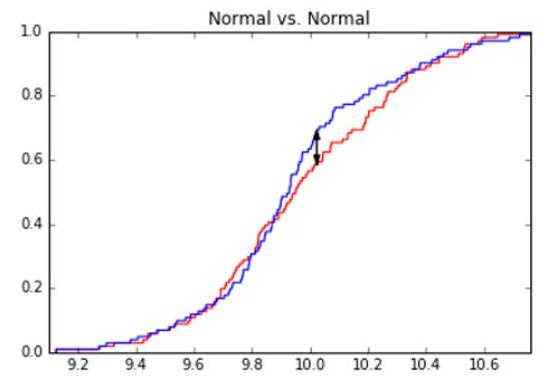
\includegraphics[max width=\textwidth]{2025_03_17_ca60ec0bfd96dcf8e028g-156}
    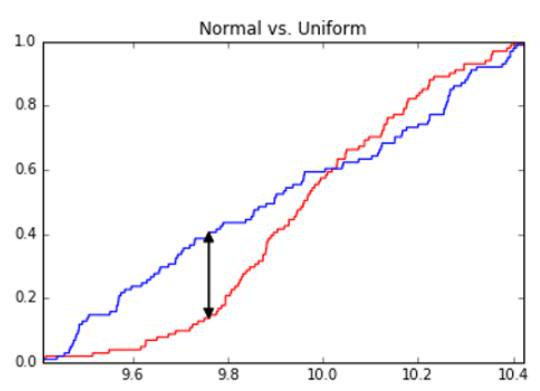
\includegraphics[max width=\textwidth]{2025_03_17_ca60ec0bfd96dcf8e028g-156(1)}
    \caption{The Kolmogorov-Smirnov \textenglish{test} \textenglish{quantifies} \textenglish{the} \textenglish{difference} \textenglish{between} \textenglish{two} \textenglish{probability} \textenglish{distributions} \textenglish{by} \textenglish{the} \textenglish{maximum} $y$-distance \textenglish{gap} \textenglish{between} \textenglish{the} \textenglish{two} \textenglish{cumulative} \textenglish{distribution} functions. \textenglish{On} \textenglish{the} left, \textenglish{two} \textenglish{samples} \textenglish{from} \textenglish{the} \textenglish{same} \textenglish{normal} distribution. \textenglish{On} \textenglish{the} right, \textenglish{comparison} \textenglish{of} \textenglish{samples} \textenglish{from} \textenglish{uniform} \textenglish{and} \textenglish{normal} \textenglish{distributions} \textenglish{drawn} \textenglish{over} \textenglish{the} \textenglish{same} $x$-range.}\index{decision boundaries}\index{logit function}\index{regression!logistic}
    \label{fig:ks-test}
\end{figure}

वितरणों को सीडीएफ़ (\textenglish{cdfs}) के रूप में प्रदर्शित किया जाता है, जहाँ\(y\)-अक्ष संचयी संभावना को 0 से 1 तक दर्शाता है। दोनों फ़ंक्शन बाएँ से दाएँ एकसमान रूप से बढ़ते हैं, जहाँ \(C(\textenglish{x})\) नमूने\(\leqx\) का अंश है।

हम उस\(x\)के मान को पहचानने की कोशिश कर रहे हैं जिसके लिए दोनों \textenglish{cdfs} के संबंधित\(y\)मूल्यों में जितना संभव हो उतना भिन्नता हो। वितरणों\(C_{1}\leftऔर\rightC_{2}\)के बीच की दूरी\(D\)(C_{1}, C_{2}\()\)इस महत्वपूर्ण\(x\)पर\(y\)मूल्यों का अंतर है, जिसे औपचारिक रूप से निम्नलिखित रूप में व्यक्त किया गया है।

\[
D\left(C_{1}, C_{2}\right)=\max_{-\infty \leq \textenglish{x} \leq \infty}\left|C_{1}(\textenglish{x})-C_{2}(\textenglish{x})\right|
\]

जितना अधिक दो नमूना वितरण कुछ मान पर भिन्न होते हैं, उतना ही अधिक संभावना होती है कि वे विभिन्न वितरणों से खींचे गए हों। चित्र\ref{आकृति:ks-test}(बाएं) दिखाता है कि समान सामान्य वितरण से दो स्वतंत्र नमूने। दोनों के बीच उत्पन्न हुई छोटी खाई पर ध्यान दें। इसके विपरीत, चित्र\ref{आकृति:ks-test}(दाएं) एक सामान्य वितरण से खींचे गए नमूने की तुलना समान वितरण से खींचे गए नमूने से करता है। KS- परीक्षण मूर्ख नहीं बनता: पूंछ के पास बड़ी खाइयाँ देखें, जहाँ हम इसे देखने की अपेक्षा करेंगे।

केएस-टेस्ट काॅम्पेयर करता है \(D\left(C_{1}, C_{2}\right)\) के मान को एक विशेष लक्ष्य के विरुद्ध, यह बताते हुए कि दो वितरण एक महत्व स्तर पर भिन्न होते हैं \(\alpha\) जब:

\[
D\left(C_{1}, C_{2}\right)>c(\alpha) \sqrt{\frac{n_{1}+n_{2}}{n_{1} n_{2}}}
\]

जहाँ\(c(\alpha)\)एक स्थिरांक है जिसे एक तालिका में देखा जाता है। नमूना आकार के कार्य के पीछे कुछ अंतर्ज्ञान है। सरलता के लिए मान लें कि दोनों नमूनों का आकार समान है,\(n\)। फिर

\[
\sqrt{\frac{n_{1}+n_{2}}{n_{1} n_{2}}}=\sqrt{\frac{2 n}{n^{2}}}=\sqrt{\frac{2}{n}}
\]

मात्रा\(\sqrt{n}\)स्वाभाविक रूप से नमूना समस्याओं में उत्पन्न होती है, जैसे बायनोमियल वितरण का मानक विचलन।\(n\)सिक्के के उछालों में सिर और पूंछ की संख्या के बीच अपेक्षित अंतर\(\sqrt{n}\)के क्रम में होता है। KS-परीक्षण के संदर्भ में, यह समान रूप से दर्शाता है कि जब दो नमूनों को समान माना जाना चाहिए तो अपेक्षित विचलन को दर्शाता है। KS-परीक्षण वितरण के सार में क्या हो रहा है, उसे दर्शाता है, जहाँ एक मजबूत निर्धारण किया जा सकता है।\index{loss function}

मुझे कोलमोगोरोव-समीरनोव परीक्षण पसंद है। यह वितरणों की तस्वीरें प्रदान करता है जिन्हें मैं समझ सकता हूँ, जो इस धारणा के सबसे कमजोर बिंदु की पहचान करती हैं कि वे समान हैं। इस परीक्षण में t-परीक्षण की तुलना में तकनीकी धारणाएँ और विविधताएँ कम होती हैं, जिसका अर्थ है कि इसे उपयोग करते समय गलती करने की संभावना कम होती है। और KS-परीक्षण को कई समस्याओं पर लागू किया जा सकता है, जिसमें यह जांचना भी शामिल है कि क्या बिंदु सामान्य वितरण से खींचे गए हैं।

\section{साधारणता परीक्षण}
\index{normality testing}जब ग्राफ पर चित्रित किया जाता है, तो साधारण वितरण एक घंटी के आकार का \index{bell-shaped}वक्र बनाता है। लेकिन हर घंटी के आकार का वितरण साधारण नहीं होता, और कभी-कभी यह जानना महत्वपूर्ण होता है कि अंतर क्या है।

दिए गए वितरणीय नमूनों\(f_{1}\)की सामान्यता परीक्षण के लिए विशेष सांख्यिकीय परीक्षण मौजूद हैं। लेकिन हम इस काम को करने के लिए सामान्य KS-परीक्षण का उपयोग कर सकते हैं, बशर्ते हम एक अर्थपूर्ण\(f_{2}\)को पहचान सकें जिससे\(f_{1}\)की तुलना की जा सके।

यही कारण है कि मैंने सेक्शन 5.2 में रैंडम सैम्पलिंग मैथड्स को प्रस्तुत किया। हमारे द्वारा वर्णित क्यूम्युलेटिव डिस्ट्रीब्यूशन मैथड का उपयोग करके, किसी भी वितरण से सांख्यिकीय रूप से सही रैंडम सैम्पल \(n\) पॉइंट्स के लिए प्राप्त किए जा सकते हैं, बशर्ते आपको उस वितरण का \textenglish{cdf} पता हो, किसी भी \(n\) के लिए। \(f_{2}\) के लिए, हमें तुलना करने के लिए पॉइंट्स की एक अर्थपूर्ण संख्या चुननी चाहिए। हम \(n_{2}=n_{1}\) का उपयोग कर सकते हैं, या शायद \(n_{1}\) बहुत छोटा होने पर कुछ बड़ा सैम्पल ले सकते हैं। हम सुनिश्चित करना चाहते हैं कि हम अपने सैम्पल के माध्यम से वांछित वितरण के आकार को सही ढंग से समझ रहे हैं।

इसलिए यदि हम सामान्य वितरण के लिए अपने यादृच्छिक नमूने का निर्माण करते हैं\(f_{2}\)से, तो KS-परीक्षण को\(f_{1}\)और\(f_{2}\)में अंतर करने में सक्षम नहीं होना चाहिए यदि\(f_{1}\)भी उसी\(\mu\)और\(\sigma\)पर एक सामान्य वितरण से आता है।

एक चेतावनी का शब्द। पर्याप्त संवेदनशील सांख्यिकीय परीक्षण संभवतः किसी भी देखे गए वितरण की सामान्यता को अस्वीकार कर देगा। सामान्य वितरण एक निरूपण है, और दुनिया एक जटिल जगह है। लेकिन ⸨KS-test⸩ के ग्राफ को देखकर आप यह जान सकते हैं कि भिन्नताएँ कहाँ हो रही हैं। क्या पूँछें बहुत मोटी हैं या बहुत पतली? क्या वितरण तिरछा है? इस समझ के साथ, आप तय कर सकते हैं कि भिन्नताएँ आपके लिए मायने रखने के लिए पर्याप्त बड़ी हैं या नहीं।

\subsection{बोनफरोनी सुधार}
\index{Bonferroni correction}विज्ञान में यह लंबे समय से प्रचलन रहा है कि\(\alpha=0.05\)को सांख्यिकीय महत्व और अप्रासंगिकता के बीच की सीमा के रूप में उपयोग किया जाता है। 0.05 की सांख्यिकीय महत्वता का अर्थ है कि यह संभावना है कि\(1 / 20\)इस परिणाम के केवल संयोग से होने की संभावना है।\index{overfitting}

यह एक अनुचित मानक नहीं है जब एक चुनौतीपूर्ण परिकल्पना का परीक्षण करने के लिए डेटा एकत्र किया जा रहा हो। 20 से 1 के समीकरण पर किसी घोड़े पर दांव लगाना और अपनी बाजी जीतना एक उल्लेखनीय उपलब्धि है। जब तक कि आपने एक ही समय में लाखों अन्य घोड़ों पर दांव नहीं लगाया हो। फिर \(20-1\)बाज़ियों की कम संख्या के बारे में डींग मारना जहाँ आप वास्तव में जीते थे, कम से कम कहने के लिए, भ्रामक होगा।

इसलिए मछली पकड़ने के अभियान जो लाखों परिकल्पनाओं का परीक्षण करते हैं, उन्हें उच्च मानकों पर रखा जाना चाहिए। यह वह भ्रांति है जिसने चित्र 5.10 में कंप्यूटर विज्ञान पीएच.डी. और वीडियो गेम गतिविधि के बीच मजबूत लेकिन जाली सहसंबंध बनाया। यह हजारों समय श्रृंखलाओं की एक-दूसरे से तुलना करते हुए खोजा गया, और केवल सबसे मनोरंजक सुनाई देने वाले जोड़ों को बनाए रखा गया जो एक उच्च सहसंबंध स्कोर दिखाने के लिए हुआ।\index{classification!multi-class}\index{scale invariant!ordinal}

द बोंफेरोनी करेक्शन\footnote{मैंने हमेशा सोचा है कि "द बोंफेरोनी करेक्शन" एक एक्शन मूवी के लिए एक शानदार शीर्षक बनेगा। ड्वेन जॉनसन बोंफेरोनी के रूप में?}हमारे विश्वास के संतुलन को एक महत्वपूर्ण संतुलन प्रदान करता है कि हम कितने भरोसेमंद माने गए सांख्यिकी परिणाम पर भरोसा करते हैं। यह इस तथ्य को दर्शाता है कि आप सहसंबंध कैसे पाए गए हैं, यह स्वयं सहसंबंध की ताकत जितना ही महत्वपूर्ण हो सकता है। कोई व्यक्ति जो एक मिलियन लॉटरी टिकट खरीदता है और एक बार जीतता है, उसके पास उस साथी की तुलना में बहुत कम प्रभावशाली मोजो होता है जो एक ही टिकट खरीदता है और जीत जाता है।\index{scale invariant!Likert}

दि बोनफेरोनि करेक्शन कहता है कि जब विभिन्न परिकल्पनाओं की एक साथ जांच की जाती है, तो परिणामी\(p\)-मूल्य को महत्वपूर्ण मानने के लिए\(\)/ n\( के स्तर तक बढ़ना चाहिए, ताकि इसे\alpha\)\(स्तर पर महत्वपूर्ण माना जा सके।

किसी भी सांख्यिकीय परीक्षण की तरह, सुधार को सही तरीके से लागू करने में कई सूक्ष्मताएँ छुपी हो सकती हैं। लेकिन यहाँ का मुख्य सिद्धांत समझना महत्वपूर्ण है। कंप्यूटर लोग विशेष रूप से सभी चीजों के खिलाफ सभी चीजों का बड़ा पैमाने पर तुलना करने या असामान्य अपवाद और पैटर्न की खोज करने के लिए प्रवृत्त होते हैं। आखिरकार, एक बार जब आप विश्लेषण प्रोग्राम लिख लेते हैं, तो इसे अपने सभी डेटा पर क्यों न चलाएं? केवल सबसे अच्छे, चुने हुए परिणाम प्रस्तुत करने से दूसरों को धोखा देना आसान हो जाता है। बॉनफेरोनी शुद्धि आपके लिए खुद को धोखा देने से रोकने का तरीका है।

\subsection{गलत खोज दर}
बॉनफेरोनी सुधार हमें कई परीक्षणों में से एक अकेली सफल परिकल्पना की महत्वपूर्णता को जल्दी मान लेने से सुरक्षित रखता है। लेकिन अक्सर जब हम बड़े, उच्च-आयामी डेटा के साथ काम करते हैं, तो हम एक अलग समस्या का सामना करते हैं। शायद सभी\(m\) चर (शायद कमजोर रूप से) लक्ष्य चर के साथ सम्बन्धित होते हैं। अगर\(n\) काफी बड़ा है, तो इनमें से कई संबंध सांख्यिकीय रूप से महत्वपूर्ण होंगे। क्या हमने वास्तव में इतनी सारी महत्वपूर्ण खोजें की हैं?\index{Bayes’ theorem}\index{decision \textenglish{tree} classifiers}\index{multinomial regression}\index{partition function}

बेंजामिनी-होचबर्ग प्रक्रिया झूठी खोज दर (एफडीआर) को न्यूनतम करने की प्रक्रिया के लिए एक बहुत ही सरल तरीका प्रदान करती है, जो महत्वपूर्णता के आधार पर दिलचस्प और नीरस चर के बीच की सीमा रेखा खींचने की अनुमति देती है। चर को उनके\(p\)-मूल्य की ताकत के अनुसार क्रमबद्ध करें, ताकि अधिक चरम चर बाईं ओर हों, और सबसे कम महत्वपूर्ण चर दाईं ओर हों। अब इस क्रम में\(i\)वें स्थान वाले चर पर विचार करें। हम इस चर की महत्वपूर्णता को उस\(\alpha\)स्तर पर स्वीकार करते हैं यदि

\[
\forall_{j=1}^{i}\left(p_{j} \leq \frac{j}{m} \alpha\right)
\]

%---- \textenglish{Page} \textenglish{End} \textenglish{Break} \textenglish{Here} ---- \textenglish{Page} : 142

\section{युद्ध कहानी: युवा स्रोत की खोज?}

\begin{figure}[ht]
\centering
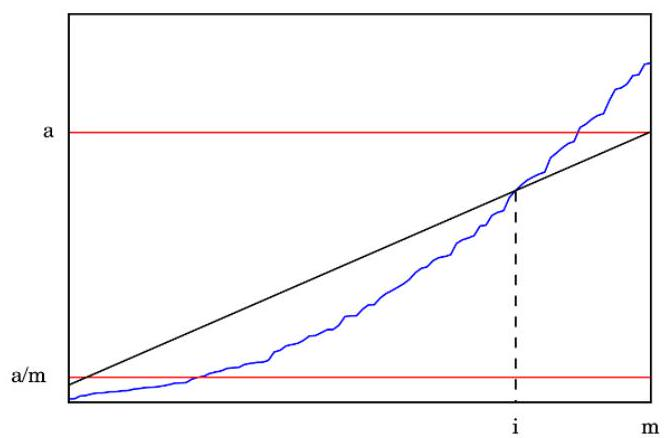
\includegraphics[max width=\textwidth]{2025_03_17_ca60ec0bfd96dcf8e028g-159}
\caption{The Benjamini-Hochberg \textenglish{procedure} \textenglish{minimizes} \textenglish{false} \textenglish{discovery} rate, \textenglish{by} \textenglish{accepting} $p$-values \textenglish{only} \textenglish{when} $p_{i} \leq \alpha \textenglish{i} / m$. \textenglish{The} \textenglish{blue} \textenglish{curve} \textenglish{shows} \textenglish{the} \textenglish{sorted} $p$ values, \textenglish{and} \textenglish{the} \textenglish{diagonal} \textenglish{defines} \textenglish{the} \textenglish{cutoff} \textenglish{for} \textenglish{when} \textenglish{such} \textenglish{a} $p$-value \textenglish{is} significant.}
\end{figure}

स्थिति को चित्र 5.14 में दिखाया गया है। $p$-मूल्यों को बाएँ से दाएँ बढ़ते क्रम में श्रेणीबद्ध किया गया है, जैसा कि अनियमित नीली वक्र द्वारा इंगित किया गया है। यदि हम सभी $p$-मूल्यों को स्वीकार कर रहे थे जो $\alpha$ से कम हैं, तो हम बहुत अधिक स्वीकार कर रहे होते। यही कारण है कि \textenglish{Bonferroni} ने अपने संशोधन को विकसित किया। लेकिन सभी $p$-मूल्यों को \textenglish{Bonferroni} संशोधन के मानक (जहाँ वक्र $\alpha$/ m@ पर पार करता है) को पूरा करने की आवश्यकता अत्यधिक कड़े है।

बेंजामिनी-होखबर्ग प्रक्रिया यह मान्यता देती है कि यदि कई मान एक विशेष मानक के लिए वास्तव में महत्वपूर्ण हैं, तो उनमें से एक निर्धारित भाग को बहुत उच्च मानक के लिए महत्वपूर्ण होना चाहिए। चित्र 5.14 में विकर्ण रेखा इस गुणवत्ता नियंत्रण के स्तर को सही ढंग से लागू करती है।

यह एक सुंदर शादी थी। हम रेचल और डेविड, दुल्हन और दूल्हे के लिए बहुत खुश थे। मैंने राजा की तरह भोजन किया था, अपनी प्यारी पत्नी के साथ नृत्य किया था, और तब तक प्राइम रिब की गर्माहट का आनंद ले रहा था जब अचानक मुझे एहसास हुआ कि कुछ गड़बड़ है। मैंने कमरे के चारों ओर देखा और दोबारा देखा। किसी तरह, कई वर्षों में पहली बार, मैं भीड़ में अधिकांश लोगों से छोटा हो गया था।

यह आपको इतना बड़ी बात नहीं लग सकती, लेकिन इसका कारण यह है कि आप, पाठक, शायद\textit{हो}कई परिस्थितियों में अधिकांश लोगों से कम उम्र के हैं। लेकिन मुझ पर विश्वास करें, ऐसा समय आएगा जब आप ऐसी चीजों को नोटिस करेंगे। मुझे याद है जब मैंने पहली बार महसूस किया कि जब में कॉलेज जा रहा था, तब मेरे अधिकांश छात्र पैदा हो रहे थे। फिर वे उस समय पैदा होने लगे जब मैं स्नातक स्कूल में था। आज के कॉलेज के छात्र न केवल उस समय के बाद पैदा हुए जब मैं प्रोफेसर बना, बल्कि उस समय बाद जब मुझे यहाँ स्थायी पद मिला। तो मैं इस शादी में अधिकांश लोगों से कम उम्र का कैसे हो सकता हूँ?

वहाँ दो संभावनाएँ थीं। या तो यह संयोगवश था कि इतने सारे वृद्ध लोग कमरे में प्रवेश कर गए, या फिर इस घटना को समझाने के लिए कोई कारण था। यही कारण है कि सांख्यिकीय महत्व परीक्षण (\textenglish{statistical} \textenglish{significance} \textenglish{tests}) और $p$-मूल्य (p-values) का आविष्कार किया गया, जो कुछ को कुछ नहीं से अलग करने में सहायता करते हैं।

तो उस समय, जब मेरी उम्र 54 वर्ष थी, रैचल की शादी में उपस्थित 251 लोगों में से अधिकतर लोगों से मैं कम उम्र का था, इसकी संभावना कितनी थी? वोल्फ्राम अल्फा के अनुसार \index{Wolfram Alpha}(विशेष रूप से, 2008-2012 के अमेरिकी सामुदायिक सर्वेक्षण के पाँच वर्षीय अनुमान), संयुक्त राज्य अमेरिका में 309.1 मिलियन लोग थे, जिनमें से 77.1 मिलियन 55 वर्ष या उससे अधिक उम्र के थे। लगभग सटीक$25\%$जनसंख्या मुझसे बड़ी है जब मैं ये शब्द लिख रहा हूँ।

251 बेतरतीब ढंग से चुने गए अमेरिकियों में से बहुमत के 55 वर्ष से अधिक आयु के होने की संभावना इस प्रकार दी गई है:

$$
\textenglish{p} =\sum_{i=126}^{251}\binom{251}{i}(1-0.75)^{i}(0.75)^{(251-i)}= 8.98\times10^{-18}
$$

यह संभावना असंभव रूप से छोटी है, इस तरह जैसे अपनी जेब से एक निष्पक्ष सिक्का निकालना और उसे 56 बार लगातार हेड्स आना। यह एक संयोग घटना का परिणाम नहीं हो सकता था। कोई निश्चित कारण था कि मैं इस भीड़ के अधिकांश लोगों से कनिष्ठ था, और इसका उत्तर यह नहीं था कि मैं और युवा हो रहा था।

जब मैंने रेचेल से इसके बारे में पूछा, तो उसने बताया कि बजट के कारण, उन्होंने शादी में बच्चों को निमंत्रण न देने का निर्णय लिया। यह एक उचित स्पष्टीकरण हो सकता है। आखिरकार, इस नियम के तहत शादी में भाग लेने से अठारह वर्ष से कम उम्र के 73.9 मिलियन लोगों को बाहर रखा गया था, जिससे उन सभी को आमंत्रित करने की लागत से अरबों डॉलर बच गए। मुझसे छोटे लोगों का चर हिस्सा$f$जो बच्चे नहीं हैं, यह इस प्रकार है$f = 1 - (77.1 / (309.1 - 73.9)) = 0.672$। हालांकि, यह 0.5 से काफी बड़ा है। इस समूह से लिए गए अनियमित नमूने में मेरे माध्य से छोटी उम्र होने की संभावना है:

$$
\textenglish{p} =\sum_{i=126}^{251}\binom{251}{i}(1-0.0672)^{i}(0.672)^{(251-i)}= 9.118\times10^{-9}
$$

हालांकि यह पहले के$p$-value से बहुत बड़ा है, यह अब भी असंभव रूप से छोटा है: जैसे आपकी निष्पक्ष सिक्के पर 27 बार लगातार हेड्स आना। केवल बच्चों को मना करना मुझे फिर से जवान बनाने के लिए पर्याप्त नहीं था।

मैं रैचल के पास वापस गया और उससे सच उगलवाया। पता चला कि उसकी माँ के बचपन में असामान्य रूप से बहुत सारे चचेरे भाई-बहन थे, और वह \textit{सब}के संपर्क में रहने में बेहद अच्छी थीं। आइंस्टीन के सापेक्षता के सिद्धांत को याद कीजिए,\index{theory \textenglish{of} relativity} जहाँ पर$E=mc^{2}$दर्शाता है कि हर कोई मेरी माँ का दो बार हटाया गया चचेरा भाई-बहन है। ये \textit{सब}चचेरे भाई-बहन शादी में आमंत्रित थे। रैचल के परिवार के दूल्हे के असामान्य रूप से छोटे समूह की तुलना में अधिक संख्याबल होने के कारण, इन वरिष्ठ चचेरे भाई-बहनों के समूह ने नृत्य स्थल पर प्रभुत्व जमा लिया।

वास्तव में, हम उन बड़े-कजिन्स की संख्या ($c$) की गणना कर सकते हैं जिन्हें आमंत्रित करना होगा ताकि यह सुनिश्चित हो सके कि मैं आमंत्रित मेहमानों के माध्य बतौर न्यूनतम आयु वाला व्यक्ति रहूँ, अगर बाकी 251 मेहमानों का चयन रैन्डम तरीक़े से किया गया हो। यह निष्कर्ष निकलता है कि

%---- \textenglish{Page} \textenglish{End} \textenglish{Break} \textenglish{Here} ---- \textenglish{Page} : 144
\clearpage 
\section{Permutation \textenglish{Tests} \textenglish{and} P-values}

\begin{figure}[htbp]
    \centering
    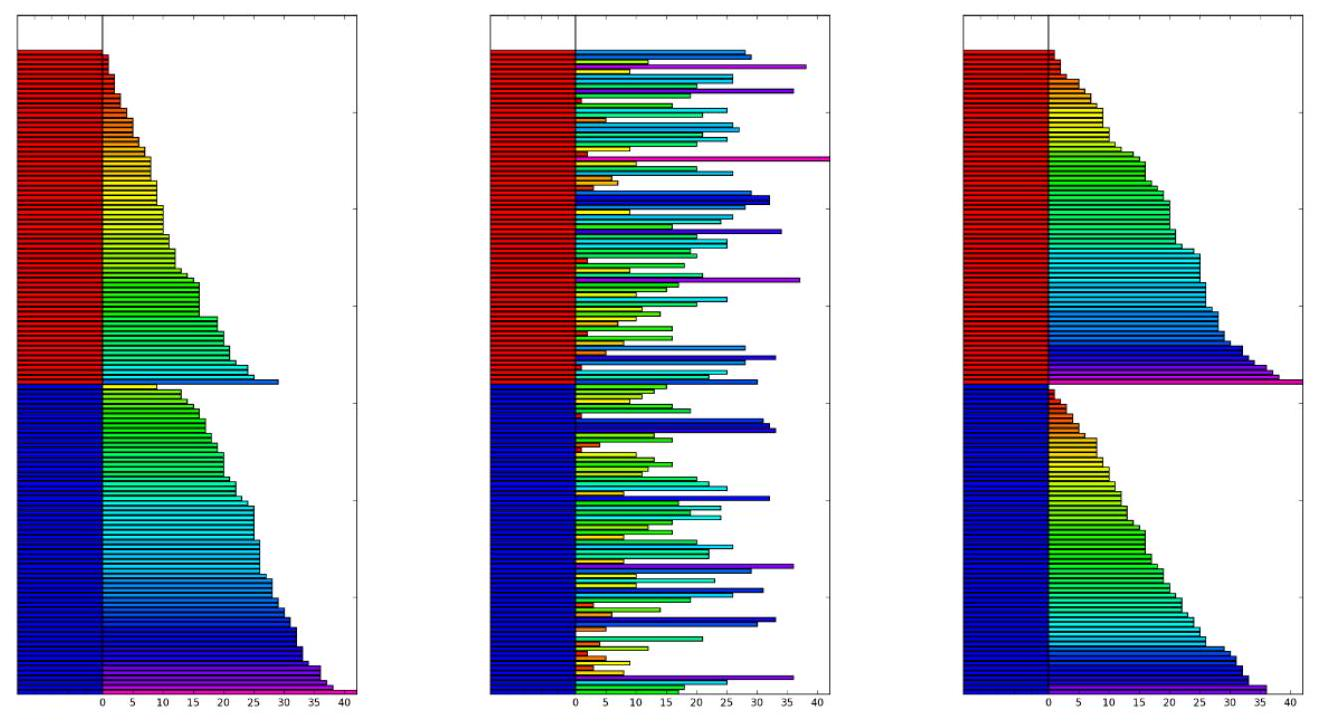
\includegraphics[max width=\textwidth]{2025_03_17_ca60ec0bfd96dcf8e028g-161}
    \caption{Permutation \textenglish{tests} \textenglish{reveal} \textenglish{the} \textenglish{significance} \textenglish{of} \textenglish{the} \textenglish{correlation} \textenglish{between} \textenglish{gender} \textenglish{and} \textenglish{the} \textenglish{height} (\textenglish{left}). \textenglish{A} \textenglish{random} \textenglish{assignment} \textenglish{of} \textenglish{gender} \textenglish{to} \textenglish{height} (\textenglish{center}) \textenglish{results} \textenglish{in} \textenglish{a} \textenglish{substantially} \textenglish{different} \textenglish{distribution} \textenglish{of} \textenglish{outcomes} \textenglish{when} \textenglish{sorted} (\textenglish{right}), \textenglish{validating} \textenglish{the} \textenglish{significance} \textenglish{of} \textenglish{the} \textenglish{original} relationship.}
\end{figure}

मूल्य$c=65$अकेले चचेरे भाई (या 32.5 विवाहित जोड़े) पर्याप्त होते हैं, जब बच्चों को बाहर रखा जाता है ($f=0.672$)।

यहाँ नैतिक यह है कि किसी भी रोचक अवलोकन को चमत्कार घोषित करने से पहले उसकी प्रायिकता की गणना करना महत्वपूर्ण है। यदि कोई आंशिक व्याख्या आश्चर्य को संभावित स्तरों तक नहीं घटाती है, तो वहीं नहीं रुकें। संभवतः किसी भी पर्याप्त दुर्लभ घटना के नीचे एक वास्तविक घटना होती है, और यह पता लगाना कि वह क्या है, डेटा विज्ञान को रोमांचक बनाता है।\index{distance metrics}\index{metric}\index{metric!identity}\index{metric!positivity}\index{metric!symmetry}\index{metric!triangle inequality}\index{distance metrics!euclidean}\index{distance metrics!manhattan distance}\index{distance metrics!maximum component}

पारंपरिक सांख्यिकीय महत्व परीक्षण यह निर्णय लेने में काफी प्रभावी साबित होते हैं कि क्या दो नमूने वास्तव में एक ही वितरण से लिए गए हैं। हालाँकि, इन परीक्षणों को सही ढंग से करने की आवश्यकता होती है ताकि वे अपना कार्य कर सकें। कई मानक परीक्षणों में सूक्ष्मताएँ होती हैं जैसे कि एक-पक्षीय बनाम दो-पक्षीय परीक्षण, वितरणिक मान्यताएँ, और भी बहुत कुछ। इन परीक्षणों को सही तरीके से करना सावधानी और प्रशिक्षण की आवश्यकता होती है।

\textit{पर्मुटेशन टेस्ट}एक अधिक सामान्य और कंप्यूटेशनली मूर्खता-सबूत तरीका प्रदान करते हैं ताकि महत्व को स्थापित किया जा सके। यदि आपका परिकल्पना डेटा द्वारा समर्थित है, तो यादृच्छिक रूप से व्यवस्थित डेटा सेट होने की संभावना कम होनी चाहिए जो इसे समर्थन करते हों। यादृच्छिक किए गए डेटा के खिलाफ कई परीक्षण करने से हम बिल्कुल यह स्थापित कर सकते हैं कि आप जिस घटना का परीक्षण कर रहे हैं वह कितना असामान्य है।

\begin{figure}[htbp]
    \centering
    \includegraphics[max width=\textwidth]{2025_03_17_ca60ec0bfd96dcf8e028g-162(1)}\\
    \includegraphics[max width=\textwidth]{2025_03_17_ca60ec0bfd96dcf8e028g-162}
    \caption{Permutation \textenglish{tests} \textenglish{score} \textenglish{significance} \textenglish{by} \textenglish{the} \textenglish{position} \textenglish{of} \textenglish{the} \textenglish{score} \textenglish{on} \textenglish{actual} \textenglish{data} \textenglish{against} \textenglish{a} \textenglish{distribution} \textenglish{of} \textenglish{scores} \textenglish{produced} \textenglish{by} \textenglish{random} permutations. \textenglish{A} \textenglish{position} \textenglish{on} \textenglish{the} \textenglish{extreme} \textenglish{tail} (\textenglish{left}) \textenglish{is} \textenglish{highly} significant, \textenglish{but} \textenglish{one} \textenglish{within} \textenglish{the} \textenglish{body} \textenglish{of} \textenglish{the} \textenglish{distribution} (\textenglish{left}) \textenglish{is} uninteresting.}
\end{figure}

चित्र\ref{fig:5.15} पर विचार करें, जहाँ हम स्वतंत्र चर (लिंग: पुरुष या महिला) और आश्रित चर (जैसे, ऊँचाई) का संकेत रंगों के माध्यम से करते हैं। मूल परिणाम रंग वितरण (बाएँ) पुरुषों और महिलाओं के बीच स्पष्ट रूप से अलग दिखाई देता है, जो ऊँचाई में वास्तविक अंतर को दर्शाता है। लेकिन यह अंतर कितना असामान्य है? हम एक नया डेटा सेट बना सकते हैं जिसमें मूल परिणाम चर को यादृच्छिक रूप से लिंग सौंप दिया जाता है (केंद्र)। प्रत्येक समूह के भीतर क्रमबद्ध करने से स्पष्ट होता है कि परिणामों का छद्म-पुरुष/महिला वितरण अब मूल डेटा (दाईं ओर) की तुलना में कहीं अधिक संतुलित है। इससे यह साबित होता है कि लिंग\textit{वास्तव में} ऊँचाई निर्धारित करने में एक महत्वपूर्ण कारक था, एक निष्कर्ष जिसे हम और भी दृढ़ता से मानने लगेंगे जब ऐसा 1,000 या$1,000,000$परीक्षणों में बार-बार होता रहेगा।

परीक्षण सांख्यिकी के वास्तविक डेटा पर रैंक, यादृच्छिक क्रम-बदल के सांख्यिकी मानों के वितरण में, महत्व स्तर या\textit{p-मूल्य} को निर्धारित करता है। आकृति\ref{fig:5.16}(बाएँ) में यह दर्शाया गया है कि हम क्या खोज रहे हैं। वास्तविक मान वितरण के सबसे दाएँ हिस्से में होता है, जो महत्व को प्रमाणित करता है। दाईं ओर की आकृति में, वास्तविक मान वितरण के मध्यम स्थान पर होता है, जो किसी प्रभाव का सुझाव नहीं देता।

परम्युटेशन परीक्षणों के लिए आपके द्वारा आंकड़ों के बारे में जो परिकल्पना है, उसे प्रतिबिंबित करने वाले एक आंकड़े विकसित करना आवश्यक है। यदि आप किसी विशिष्ट युग्म के बीच एक महत्वपूर्ण संबंध स्थापित करना चाहते हैं, तो कोरिलेशन कोएफिशिएंट एक उचित विकल्प है। आदर्श रूप से, वास्तविक आंकड़ों में प्रेक्षित कोरिलेशन इसके किसी भी यादृच्छिक परम्युटेशन के मुकाबले अधिक मजबूत होगा। लिंग-ऊंचाई संबंध को मान्य करने के लिए, शायद हमारा आंकड़ा पुरुषों और महिलाओं की औसत ऊंचाई में अंतर हो सकता है। फिर से, हम आशा करते हैं कि यह वास्तविक आंकड़ों में इसके अधिकांश यादृच्छिक परम्युटेशनों से बड़ा साबित होता है।

आपकी सांख्यिकी के चयन में सृजनशील बनें: परमीटेशन परीक्षणों की शक्ति यह है कि वे लगभग किसी भी चीज के साथ कार्य कर सकते हैं जिसे आप अपने मामले को साबित करने के लिए लेकर आते हैं। यह सबसे अच्छा होगा यदि आपकी सांख्यिकी समता के अवसर को कम से कम करें, क्योंकि आपको अपने परिकल्पना के खिलाफ सभी समताएं गिनने का कर्तव्य निभाना होता है।

\textit{घर पर सीखने के लिए पाठ:}पर्म्यूटेशन टेस्ट आपको आपके डेटा की संभावना देते हैं आपके परिकल्पना के अनुसार, अर्थात् यह सांख्यिकी यादृच्छिक नमूना वितरण की तुलना में एक अपवाद होगा। यह आपके डेटा के आधार पर आपकी परिकल्पना को साबित करने के समान नहीं है, जो सांख्यिकीय महत्व परीक्षण का पारंपरिक लक्ष्य है। लेकिन यह कुछ भी नहीं से बहुत बेहतर है।

परिवर्तन परीक्षण का महत्व स्कोर या \textit{p-value} इस बात पर निर्भर करता है कि कितने यादृच्छिक प्रयास किए जाते हैं। हमेशा कम से कम 1,000 यादृच्छिक परीक्षण करने की कोशिश करें, और अधिक यदि यह संभव हो। जितनी अधिक \textenglish{permutations} आप प्रयास करेंगे, उतना ही प्रभावशाली आपका महत्व \textit{p-value} हो सकता है, एक निश्चित बिंदु तक। यदि दिया गया इनपुट वास्तव में सभी $k$! \textenglish{permutations} में से सबसे अच्छा है, तो सबसे चरम \textit{p-value} जो आप प्राप्त कर सकते हैं वह है $1/k$!, भले ही आप कितनी भी यादृच्छिक \textenglish{permutations} प्रयास करें। अधिक नमूना लेने से आपके डिनोमिनेटर को बढ़ाएगा, बिना आपके वास्तविक विश्वास को एक बिट भी बढ़ाए।

\textit{घर ले जाने का पाठ:}P-मूल्य की गणना आपके भरोसे को बढ़ाने के लिए की जाती है कि एक अवलोकन वास्तविक और दिलचस्प है। यह तभी काम करता है जब आप \textenglish{permutation} \textenglish{test} ईमानदारी से करते हैं, उन प्रयोगों को करके जो आश्चर्य का एक सही माप प्रदान कर सकते हैं।

\subsection{यादृच्छिक क्रमचय उत्पन्न करना}

रैंडम परिव्युत्पन्न उत्पन्न करना एक और महत्वपूर्ण सैंपलिंग समस्या है जिसे लोग अक्सर गड़बड़ कर देते हैं। नीचे दिए गए दो एल्गोरिदम दोनों प्रारंभिक परिव्युत्पन्न\(\{1,2,\ldots, n\}\) को गड़बड़ करने के लिए रैंडम स्वैप्स के अनुक्रम का उपयोग करते हैं।

लेकिन यह सुनिश्‍चित करना कि सभी$n$! व्यवस्थाएँ समान रूप से यादृच्छिक तरीके से उत्पन्न होती हैं, एक कठिन कार्य है। वास्तव में, इन एल्गोरिदमों में से केवल एक इसे सही करता है। क्या यह वही है,

\[\]

\begin{aligned}
& \text{के लिए } i=1 \text{से } \textenglish{n} \text{करो } a[i]=i ; \\
& \text{के लिए } i=1 \text{से } n-1 \text{करो } \operatorname{स्वैप}[a[i], a[\operatorname{रैंडम}[i, n]]] ;
\end{aligned}

\]

या क्या यह है:

\[\]

\begin{aligned}
और \text{के लिए} i=1 \text{तक} \textenglish{n} \text{करें} a[i]=i ; \\\index{dimensional egalitarianism}\index{Z-score}
और \text{के लिए} i=1 \text{तक} n-1 \text{करें} \operatorname{स्वैप}[a[i], a[\operatorname{रैंडम}[1, n]]] ;
\end{aligned}

\]

इसपर ध्यान से विचार करें: यहाँ अंतर बहुत सूक्ष्म है। यह इतना सूक्ष्म है कि आप इसे कोड में भी ध्यान नहीं देंगे। महत्वपूर्ण अंतर \textenglish{Random} के कॉल में 1 या \(i\) है। इनमें से एक एल्गोरिथम सही है और एक एल्गोरिथम गलत है। अगर आपको लगता है कि आप बता सकते हैं, तो सहमति पूर्वक समझाएं कि एक क्यों काम करता है और दूसरा क्यों नहीं करता।\index{cosine similarity}\index{norms}\index{points vs. vectors}

यदि वास्तव में आपको जानना है, तो पहला एल्गोरिद्म सही है। यह पहले स्थान के लिए 1 से \(n\) तक के किसी भी यादृच्छिक तत्व को चुनता है, फिर उसे वैसा ही छोड़ देता है और...
%---- पृष्ठ अंत ब्रेक यहां ---- पृष्ठ : 147

\begin{figure}[H]
\centering
\includegraphics[max width=\textwidth]{2025_03_17_ca60ec0bfd96dcf8e028g-164}
\caption{The \textenglish{generation} \textenglish{frequency} \textenglish{of} \textenglish{all} \(4! = 24\) \textenglish{permutations} \textenglish{using} \textenglish{two} \textenglish{different} algorithms. \textenglish{Algorithm} 1 \textenglish{generates} \textenglish{them} \textenglish{with} \textenglish{uniform} frequency, \textenglish{while} \textenglish{algorithm} 2 \textenglish{is} \textenglish{substantially} biased.}
\label{fig:permutation_frequency}
\end{figure}

बाकी पर पुनरावृत्ति होती है। यह यादृच्छिक रूप से क्रमचय उत्पन्न करता है। दूसरा एल्गोरिद्म कुछ तत्वों को पहले स्थान पर आने का बेहतर मौका देता है, यह दर्शाता है कि वितरण समरूप नहीं है।

लेकिन यदि आप इसे सैद्धांतिक रूप से प्रमाणित नहीं कर सकते हैं, तो आप प्रPermutation टेस्ट के विचार का उपयोग कर सकते हैं। दोनों एल्गोरिथ्म को लागू करें, और प्रत्येक के 1,000,000 बार रन करें, उदाहरण के लिए,\(n=4\)तत्वों की यादृच्छिक प्रPermutation का निर्माण करते समय। गिनती करें कि प्रत्येक एल्गोरिथ्म कितनी बार प्रत्येक एक\(4! = 24\)अलग-अलग प्रPermutation उत्पन्न करता है। इस तरह के प्रयोग के परिणाम चित्र\ref{fig:permutation_frequency}में दिखाए गए हैं। एल्गोरिथ्म 1 अविश्वसनीय रूप से स्थिर साबित होता है, जिसमें 166.1 घटनाओं का मानक विचलन होता है। इसके विपरीत, एल्गोरिथ्म 2 के तहत सबसे अधिक और सबसे कम सामान्य प्रPermutation के बीच आठ गुना अंतर होता है, जिसके\(\sigma= 20,923.9\)।

यहाँ नैतिकता यह है कि रैंडम जेनेरेशन बहुत सूक्ष्म हो सकता है। और मोंटे कार्लो-प्रकार के प्रयोग जैसे परम्यूटेशन टेस्ट सूक्ष्म तर्क की आवश्यकता को समाप्त कर सकते हैं। पहले सत्यापित करें, फिर विश्वास करें।

\section{दीमैगियो की हिटिंग स्ट्रीक}
बेसबॉल के सबसे अद्भुत रिकॉर्ड्स में से एक जो दीमैगियो की 56-गेम हिटिंग स्ट्रीक है। एक बल्लेबाज़ का काम है हिट्स प्राप्त करना, और उन्हें प्रत्येक गेम में शायद चार मौके मिलते हैं एक हिट पाने के लिए। यहाँ तक कि बहुत अच्छे बल्लेबाज़ भी अक्सर असफल हो जाते हैं।

लेकिन 1941 में, जो डिमैगियो ने 56 सीधे खेलों में हिट प्राप्त करने में सफलता प्राप्त की, जो वास्तव में एक अद्भुत उपलब्धि थी। तब से लेकर अब तक के पचहत्तर वर्षों में कोई खिलाड़ी इस रिकॉर्ड के करीब नहीं आया, न ही उनके पहले का कोई खिलाड़ी।

लेकिन उनके करियर के संदर्भ में इतनी लंबी लड़ी कितनी असामान्य थी? DiMag-

\begin{figure}[H]
\centering
\includegraphics[max width=\textwidth]{2025_03_17_ca60ec0bfd96dcf8e028g-165}
\caption{The \textenglish{distribution} \textenglish{of} \textenglish{longest} \textenglish{hitting} streaks, \textenglish{over} 100,000 \textenglish{simulated} careers. DiMaggio's \textenglish{actual} 56-game \textenglish{hitting} \textenglish{streak} \textenglish{stands} \textenglish{at} \textenglish{the} \textenglish{very} \textenglish{tail} \textenglish{of} \textenglish{this} distribution, \textenglish{thus} \textenglish{demonstrating} \textenglish{the} \textenglish{difficulty} \textenglish{of} \textenglish{this} feat.}
\label{fig:hitting_streaks_distribution}
\end{figure}

जियो ने 1736 खेल खेले, जिनमें 2214 हिट्स 6821 एट बैट्स में किए। अतः उसे लगभग\(1-(1-(2214 / 6821))^{4}=79.2\%\)चार एट बैट्स वाले खेल में हिट्स मिलनी चाहिए। इस स्तर की क्षमता वाले व्यक्ति के पूरे करियर में ऐसे लगातार खेलों की श्रृंखला जारी रखने की संभावना क्या है?

उन लोगों के लिए जो मेरे बेसबॉल उपमाओं से थक चुके हैं, आइए इसे एक अन्य संदर्भ में देखते हैं। मान लीजिए आप एक छात्र हैं जिसकी परीक्षाओं में औसत ग्रेड 90 है। आप निश्चित रूप से एक बहुत अच्छे छात्र हैं, लेकिन परिपूर्ण नहीं। आपके दस लगातार परीक्षाओं में 90 से अधिक अंक लाने की क्या संभावनाएं हैं? बीस लगातार परीक्षाओं का क्या? क्या आप सम्भवतः 56 परीक्षाएं लगातार पूरी तरह से कर सकते हैं?\footnotemark{}\index{Kullback-Leibler divergence}\index{nearest \textenglish{neighbor} classification}\index{nearest \textenglish{neighbor} classification!advantages}
अगर इतनी लंबी श्रंखला होती है, तो क्या इसका मतलब होगा कि आपने अपनी पढ़ाई को एक नए स्तर पर ले लिया है, या क्या आप सिर्फ किस्मत वाले थे?

तो जब \textenglish{DiMaggio} की हिटिंग स्ट्रिक थी, तो क्या यह उनकी निर्विवादित कौशल और सततता का अपेक्षित परिणाम था, या फिर वह केवल भाग्यशाली थे? वह अपने या किसी भी समय के सबसे बेहतरीन हिटर्स में से एक थे, अपने तेरह साल के करियर के हर सीजन में ऑल-स्टार। लेकिन हम यह भी जानते हैं कि कभी-कभी \textenglish{DiMaggio} भाग्यशाली भी थे। आखिरकार, वह मशहूर फिल्म स्टार \textenglish{Marilyn} \textenglish{Monroe} से शादीशुदा थे।

इस प्रश्न को हल करने के लिए, हमने यादृच्छिक संख्याओं का उपयोग किया है ताकि यह आभास दिया जा सके कि उसने 1736 खेलों के एक कृत्रिम "कैरियर" में कितनी बार हिट्स किए। प्रत्येक खेल में, सिम्युलेटेड जो को हिट करने के चार अवसर मिले, और उसे सफल होने की संभावना थी\(p=(2214/6821)=0.325\)। हम फिर इस सिम्युलेटेड करियर के दौरान सबसे लंबी हिटिंग स्ट्रीक को पहचान सकते थे। 100,000 डिमैगियो करियर के सिमुलेशन से, हम स्ट्रीक्स की एक आवृत्ति वितरण प्राप्त करते हैं, जो उसके उपलब्धि की दुर्लभता को संदर्भ में रख सकता है, प्रक्रिया में एक\(p\)-मान प्राप्त करते हुए।

परिणाम चित्र\ref{fig:hitting_streaks_distribution} में दिखाए गए हैं। केवल 44 में से 100,000 सिम्युलेशन के करियर (\(p=0.00044\)) में ही \textenglish{DiMaggio} ने कम से कम 56 खेलों की स्ट्रीक हासिल की। इस प्रकार, लंबाई उसकी अपेक्षा से काफी बाहर है। किसी भी मेजर लीग हिटर की दूसरी सबसे लंबी स्ट्रीक केवल 44 खेलों की है, इसलिए यह दूसरों के मुकाबले भी बाहर है। लेकिन उन्होंने निम्न स्तर की प्रतियोगिता में लगातार 61 खेलों में हिट किया था, इसलिए उनके पास निरंतरता की एक असाधारण क्षमता थी।\index{analogies}

हिटिंग स्ट्रीक्स को हिट्स के बिना खेलों के बीच रनों के रूप में सोचा जा सकता है, और इसलिए इन्हें पॉइसन वितरण का उपयोग करके मॉडल किया जा सकता है। लेकिन मॉन्टे कार्लो सिमुलेशन हमें बिना विस्तृत गणित के उत्तर प्रदान करते हैं। परमुटेशन टेस्ट्स हमें न्यूनतम ज्ञान और बौद्धिक प्रयास के साथ अंतर्दृष्टि देते हैं।

\section{बेयesian रीजनिंग}
सशर्त प्रायिकता\(P(A\midB)\)घटना\(A\)की संभावना को मापता है, यह जानते हुए कि घटना\(B\)घटी है। हम इस पुस्तक के दौरान सशर्त प्रायिकता पर निर्भर करेंगे, क्योंकि यह हमें ताज़ा साक्ष्यों, जैसे देखे गए डेटा के जवाब में किसी घटना पर हमारे विश्वास को अपडेट करने की अनुमति देता है।

\textit{बायज़ प्रमेय}संभावनाओं के साथ काम करने के लिए एक महत्वपूर्ण उपकरण है, क्योंकि यह हमें स्थिति को उलटने की अनुमति देता है:

\[
P(\textenglish{A} \mid \textenglish{B})=\frac{P(\textenglish{B} \mid \textenglish{A}) P(\textenglish{A})}{P(\textenglish{B})}\index{k-nearest neighbors}
\]

बेज़ का प्रमेय हमें प्रश्न को \(P(\text{परिणाम}\mid\text{डेटा})\)से \(P(\text{डेटा}\mid\text{परिणाम})\)में परिवर्तित करने की अनुमति देता है, जो अकसर गणना करने में बहुत आसान होता है। कुछ अर्थों में, बेज़ का प्रमेय सिर्फ बीजगणित का एक परिणाम है, लेकिन यह संभाव्यता के बारे में सोचने का एक अलग तरीका प्रस्तुत करता है।

\begin{figure}[H]
\centering
\includegraphics[max width=\textwidth]{2025_03_17_ca60ec0bfd96dcf8e028g-166}
\caption{Bayes' \textenglish{Theorem} \textenglish{in} action.}
\label{fig:bayes_theorem}
\end{figure}

चित्र\ref{चित्र:बेयस_सिद्धान्त}बेयस के सिद्धान्त को क्रियान्वित होते हुए दर्शाता है। घटना स्थान में चार खण्डों में से एक का चयन शामिल है। जटिल घटनाएं\(A\)और\(B\)ब्लॉकों के उप-रेंज को दर्शाती हैं, जहाँ\(P(\textenglish{A})=3/4\)और\(P(\textenglish{B})=2/4=1/2\)है। चित्र से ब्लॉकों की गणना करके, हम देख सकते हैं कि\(P(A\midB)=1/2\)और\(P(B\midA)=1/3\)हैं। ये भी सीधे बेयस के सिद्धान्त से अनुसरण करते हैं:

\[\]

\begin{aligned}
एवं P(\textenglish{A} \mid \textenglish{B})=\frac{P(\textenglish{B} \mid \textenglish{A}) P(\textenglish{A})}{P(\textenglish{B})}=\frac{(1/3) \cdot(3/4)}{(1/2)}=1/2 \\\index{classification!binary}
एवं P(\textenglish{B} \mid \textenglish{A})=\frac{P(\textenglish{A} \mid \textenglish{B}) P(\textenglish{B})}{P(\textenglish{A})}=\frac{(1/2) \cdot(1/2)}{(3/4)}=1/3
\end{aligned}

\]

बेयेसियन तर्कशास्त्र यह दर्शाता है कि एक पूर्वProbability\(P(\textenglish{A})\)को एक नई अवलोकन\(B\midके आधार पर अपडेट किया जाता है जिससे \textenglish{posterior} Probability\)P(A\(\textenglish{B})\)प्राप्त होती है, संभावना के अनुपात\(P(B\midA)\)और हाशियProbability\(P(\textenglish{B})\)के अनुसार। \textit{पूर्व Probability}\(P(\textenglish{A})\)हमारी दुनिया के प्रारंभिक अनुमान को प्रतिबिंबित करती है, जिसे अतिरिक्त प्रमाण\(B\)के आधार पर संशोधित किया जाना है।

बेयसियन रीजनिंग दुनिया को देखने का एक महत्वपूर्ण तरीका है। रैचल और डेविड की शादी में जाते समय, मेरा प्राथमिक अनुमान था कि आयु वितरण दुनिया की सामान्य स्थिति को दर्शाएगा। लेकिन मेरी आत्मविश्वास हर बुजुर्ग चचेरे भाई से मिलने के साथ कमजोर हो गई, और अंततः टूट ही गई।

हम खंड 11.1 में बेयसीयन रीजनिंग का उपयोग करके वर्गीकरणकर्ता बनाएंगे। लेकिन जब आप आंकड़ों का विश्लेषण करें, तो इस दर्शन को ध्यान में रखें। आपको प्रत्येक कार्य के लिए पहले से एक धारणा लेकर आनी चाहिए कि उत्तर क्या होने चाहिए, और फिर सांख्यिकीय सबूतों के अनुसार संशोधन करना चाहिए।\index{nearest \textenglish{neighbor} classification!finding}

\section{अध्याय नोट्स}
हर डाटा वैज्ञानिक को एक अच्छा मौलिक सांख्यिकी कोर्स करना चाहिए। प्रतिनिधिक पाठ्यों में \textenglish{Freedman} \cite{freedman2007statistics} और \textenglish{James} \textenglish{et} al. \cite{JWHT13} शामिल हैं। \textenglish{Wheelan} \cite{Whe13} एक सरल परिचय है, जबकि \textenglish{Huff} \cite{huff2010how} सांख्यिकी के साथ सबसे अच्छी तरह से झूठ बोलने पर क्लासिक ग्रंथ है।\index{kd-trees}

डोनोहो \cite{donoho2015data} आँकड़ा विज्ञान के इतिहास को एक सांख्यिकीविद् के दृष्टिकोण से प्रस्तुत करते हैं। यह प्रभावकारी रूप से यह दर्शाता है कि आज के आँकड़ा विज्ञान के अधिकतर प्रमुख सिद्धांत मूलतः सांख्यिकीविदों द्वारा विकसित किए गए थे, हालांकि उन्हें बड़े पैमाने पर इस क्षेत्र द्वारा जल्दी स्वीकृति नहीं मिली। आधुनिक सांख्यिकीविद इन मुद्दों पर कंप्यूटर वैज्ञानिकों के साथ अधिक संतोषजनक बातचीत करने लगे हैं क्योंकि रुचियाँ परस्पर अभिसरित हो गई हैं।

विजन \cite{Vig15} एक मनोरंजक संग्रह प्रस्तुत करता है जिसमें बहुत सारे दिलचस्प समय शृंखलाओं से निकाले गए झूठे सहसंबंध शामिल हैं। चित्र 5.10 इसका प्रतिनिधित्व करता है और इसे अनुमति के साथ पुनः प्रकाशित किया गया है।

यह प्रदर्शित किया गया है कि अमेरिकी परिवारों का आकार उचित रूप से पोइसन वितरण द्वारा अनुकूल है। वास्तव में, 104 देशों के घरेलू आकार के वितरण के विश्लेषण से पता चलता है कि "मैंने पर्याप्त कर लिया है" मॉडल दुनिया भर में काम करता है \cite{jennings1999household}।

\section{अभ्यास}

% Mismatched: \subsectionname{Statistical Distributions}

\item[5-2.]
\textit{[5]}निम्नलिखित \textenglish{The} \textenglish{Quant} \textenglish{Shop} घटना के लिए कौन सा वितरण सबसे उपयुक्त लगता है: बायनोमियल, नॉर्मल, पोइसन, या पावर लॉ?

\begin{itemize}
\item[(\textenglish{a})] मिस यूनिवर्स प्रतियोगिता में प्रतिभागियों की सुंदरता। 
\item[(\textenglish{b})] हॉलीवुड स्टूडियोज द्वारा निर्मित फिल्मों की कमाई। 
\item[(\textenglish{c})] नवजात शिशुओं का जन्म वजन। 
\item[(\textenglish{d})] नीलामी में कला कार्यों की कीमत। 
\item[(\textenglish{e})] क्रिसमस पर न्यूयॉर्क में गिरने वाली बर्फ की मात्रा। 
\item[(\textenglish{f})] किसी दिए गए फुटबॉल सीज़न में \(x\) खेल जीतने वाली टीमों की संख्या। 
\item[(\textenglish{g})] प्रसिद्ध लोगों की जीवन अवधि। 
\item[(\textenglish{h})] किसी दिए गए वर्ष में रोज़ सोने की कीमत। 
\end{itemize}

\item[5-3.]
\textit{[5]}मानते हुए कि संबंधित वितरण सामान्य है, निम्नलिखित घटनाओं की संभावना का अनुमान लगाएं:

\begin{itemize}
\item[(\textenglish{a})] क्या अगले सौ बार निष्पक्ष सिक्का उछालने पर 70 या उससे अधिक हेड्स आएंगे? 
\item[(\textenglish{b})] क्या एक यादृच्छिक रूप से चयनित व्यक्ति का वजन 300 पाउंड से अधिक होगा? 
\end{itemize}

\item[5-4.]
\textit{[३]}इतिहास की परीक्षा में औसत 100 में से 85 अंक था, जिसमें स्टैंडर्ड डिविएशन 15 था। क्या इस परीक्षा में स्कोर्स का वितरण सममित था? अगर नहीं, तो आप इस वितरण का कौन सा आकार अपेक्षित करते हैं? अपने तर्क की व्याख्या करें।

\item[5-5.]
\textit{[5]}फेसबुक डेटा दिखाता है कि 50\% फेसबुक उपयोगकर्ताओं के सौ या उससे अधिक मित्र हैं। इसके अलावा, औसत उपयोगकर्ता के मित्रों की संख्या 190 है। ये निष्कर्ष फेसबुक उपयोगकर्ताओं के मित्रों की संख्या के वितरण के आकार के बारे में क्या कहते हैं?
\end{enumerate}

\subsection{महत्व परीक्षण}

\begin{enumerate}
\setcounter{सूची}{5}
\item[5-6.]
\textit{[3]} निम्नलिखित घटनाओं में से कौन सी संभावित स्वतंत्र हैं और कौन सी नहीं?
\begin{itemize}
\item[(क)] सिक्का उछालना।
\end{itemize}
\end{enumerate}

\footnotetext{यदि आप मेरी कक्षाओं में से एक ले रहे हैं, तो मैं आपको बताता हूँ।}

%---- \textenglish{Page} \textenglish{End} \textenglish{Break} \textenglish{Here} ---- \textenglish{Page} : 152



\begin{enumerate}
  \setcounter{enumi}{6}
    \item 2010 की अमेरिकन कम्युनिटी सर्वेक्षण अनुमान लगाती है कि 15 वर्ष और उससे अधिक आयु की $47.1 \%$ महिलाएँ विवाहित हैं।
   \begin{enumerate}
      \item बेतरतीब ढंग से इन आयु के बीच की तीन महिलाओं का चयन करें। यह संभावना क्या है कि चयन की गई तीसरी महिला ही एकमात्र विवाहित है?
      \item यह संभावना क्या है कि सभी तीन महिलाएँ विवाहित हैं?
      \item औसतन, आप कितनी महिलाओं के नमूने लेने की उम्मीद करेंगे इससे पहले कि एक विवाहित महिला का चयन हो? मानक विचलन क्या है?
      \item यदि विवाहित महिलाओं का अनुपात वास्तव में $30 \%$ था, तो आप कितनी महिलाओं के नमूने लेने की उम्मीद करेंगे इससे पहले कि एक विवाहित महिला का चयन हो? मानक विचलन क्या है?
      \item भाग (\textenglish{c}) और (\textenglish{d}) के आपके उत्तरों के आधार पर, एक घटना की संभावना को घटाने से सफलता तक प्रतीक्षा समय का माध्य और मानक विचलन कैसे प्रभावित होते हैं?
    \end{enumerate}

\item सिद्ध करें कि पृष्ठ 147 के पर्म्यूटेशन जेनरेशन अल्गोरिद्म सही ढंग से पर्म्यूटेशन उत्पन्न करता है, अर्थात यादृच्छिक रूप से समान रूप से।

\itemm$पुरुषों और$w$महिलाओं की ऊँचाइयों से संबंधित डेटा प्राप्त करें।

\begin{enumerate}
      \item पुरुषों की औसत ऊँचाई महिलाओं से अधिक है या नहीं, इसकी महत्ता स्थापित करने के लिए t-परीक्षण का उपयोग करें।
      \item इसी चीज़ को स्थापित करने के लिए क्रमपरिवर्तन परीक्षा करें: क्या पुरुष औसतन महिलाओं से लंबे हैं।
    \end{enumerate}

\itemखेल आयोजन में, अच्छी टीमें अक्सर वापस आकर जीत जाती हैं। लेकिन क्या यह इसलिए है क्योंकि उन्हें जीतना आता है, या सिर्फ इसलिए कि लंबे समय तक चलने वाले खेल के बाद बेहतर टीम आम तौर पर जीत ही जाती है? एक रैंडम सिक्का उछाल मॉडल के साथ प्रयोग कीजिए, जहाँ बेहतर टीम के पास दूसरे पर एकल अवधि में जीतने की$संभावना प>0.5$हो। अगर खेल की$n$अवधियाँ हैं, तो बेहतर टीम कितनी बार जीतती है, और कितनी बार यह पिछड़ने के बाद जीतती है, एक दी हुई संभावना$प$के लिए? यह असली खेल की सांख्यिकी से कैसे तुलना करता है?

\itemफरवरी 2 संयुक्त राज्य अमेरिका में ग्राउंडहोग डे है, जब कहा जाता है कि यदि ग्राउंडहोग अपनी छाया देखता है तो छह और सप्ताह की सर्दी आती है। फरवरी 2 को धूप होने को ग्राउंडहोग की इनपुट के रूप में लेते हुए, क्या इस परंपरा में भविष्यवाणी की कोई शक्ति है? मौसम रिकॉर्ड के आधार पर एक अध्ययन करें, और इस जीव की भविष्यवाणियों की सटीकता के साथ इसकी सांख्यिकीय महत्वता की रिपोर्ट बनाएं।
\index{binary relations}\index{graphs!weighted}\index{matrix!adjacency}\index{networks!induced}

\section{साक्षात्कार प्रश्न}

\begin{enumerate}
  \setcounter{सूची}{11}
  \item सशर्त संभावना क्या है?
  \item बेयस प्रमेय क्या है? और व्यवहार में यह क्यों उपयोगी है?
  \item आप एक स्पैम पहचानने की एल्गोरिथ्म को कैसे सुधारेंगे जो एक साधारण बेयस वर्गीकरण का उपयोग करता है?
  \item एक सिक्का दस बार उछाला जाता है और परिणाम दो टेल्स और आठ हेड्स आते हैं। आप कैसे बता सकते हैं कि सिक्का निष्पक्ष है? इस परिणाम के लिए $p$-मूल्य क्या है?
  \item अब मान लीजिए कि दस सिक्के हैं और प्रत्येक को दस बार उछाला जाता है, कुल मिलाकर 100 बार उछालते हैं। आप कैसे परखेंगे कि सिक्के निष्पक्ष हैं?
  \item एक चींटी को एक अनंत लंबी टहनी पर रखा गया है। चींटी एक कदम पीछे या एक कदम आगे समान संभावना के साथ चल सकती है, विवेकशील समय चरणों के दौरान। चींटी के $2 n$ कदमों के बाद अपने प्रारंभिक बिंदु पर लौटने की संभावना क्या है?
  \item आप सिएटल जाने वाले विमान में चढ़ने वाले हैं। क्या आपको छाता लाना चाहिए? आप वहाँ रहने वाले अपने तीन यादृच्छिक दोस्तों को फोन करते हैं और स्वतंत्र रूप से पूछते हैं कि क्या बारिश हो रही है। प्रत्येक मित्र के पास आपको सच बताने की $2/3$ संभावना है और झूठ बोलने की $1/3$ संभावना है। सभी तीन दोस्त आपको बताते हैं कि बारिश हो रही है। यह संभावना क्या है कि वास्तव में सिएटल में बारिश हो रही है?
\end{enumerate}

% Mismatched: \sectionname{Kaggle Challenges}

\begin{enumerate}
  \setcounter{क्रम}{18}
  \item तय करें कि नीलामी में खरीदी गई कार एक खराब खरीद है या नहीं। \href{https://www.kaggle.com/c/DontGetKicked}{https://www.kaggle.com/c/DontGetKicked}
  \item एक दिए गए सप्ताह में उत्पाद की मांग का पूर्वानुमान लगाएं। \href{https://www.kaggle.com/c/grupo-bimbo-inventory-demand}{https://www.kaggle.com/c/grupo-bimbo-inventory-demand}
  \item अगले घंटे में हमें कितनी बारिश मिलेगी? \href{https://www.kaggle.com/c/how-much-did-it-rain}{https://www.kaggle.com/c/how-much-did-it-rain}
\end{enumerate}

\chapter{डेटा का चित्रण}

\epigraph{अपने श्रेष्ठ रूप में, ग्राफ़िक्स तर्क करने के उपकरण होते हैं।}{एडवर्ड टफ्टे}

प्रभावी डेटा दृश्यचित्रण डेटा विज्ञान का एक महत्वपूर्ण पहलू है, कम से कम तीन विभिन्न कारणों के लिए:\index{graphs!dense}\index{graphs!non-simple}\index{graphs!simple}\index{graphs!sparse}\index{graphs!unweighted}\index{graphs!weighted}\index{multiedge}\index{program flow graph}\index{road network}\index{self-loop}\index{simple graph}\index{unweighted graph}\index{weighted graph}

\begin{itemize}
  \item\textit{पाए खोजपरक डेटा विश्लेषण}: आपका डेटा वास्तव में कैसा दिखता है? आप जिस चीज़ से निपट रहे हैं उसका हैंडलिंग करना किसी भी गंभीर विश्लेषण का पहला कदम है। प्लॉट्स और दृश्यावलोकन यह करने का सबसे अच्छा तरीका है।
  \item\textit{त्रुटि खोज}: क्या आपने अपने विश्लेषण में कोई मूर्खतापूर्ण गलती की है? किसी मशीन लर्निंग एल्गोरिद्म को अविश्लेषित डेटा देना मुसीबत मोल लेने जैसा है। आउटलाईयर पॉइंट्स, अपर्याप्त सफाई, और गलत धारणाओं के समस्याएं आपके डेटा को सही तरीके से दृश्यावलोकन करने पर तुरंत प्रकट हो जाती हैं। अक्सर एक संक्षिप्त सांख्यिकी (77.8\% सटीकता!) छुपा लेता है कि आपका मॉडल वास्तव में क्या कर रहा है। आप जो सही कर रहे हैं और जो गलत कर रहे हैं, उस पर एक अच्छी मेहनत से नज़र डालना बेहतर प्रदर्शन करने का पहला कदम है।
  \item\textit{संचार}: क्या आप जो सीखा है उसे प्रभावी ढंग से दूसरों के सामने प्रस्तुत कर सकते हैं? अर्थपूर्ण परिणाम तब तक क्रियाशील नहीं बनते जब तक उन्हें साझा नहीं किया जाता। एक डेटा वैज्ञानिक के रूप में आपकी सफलता इस बात पर निर्भर करती है कि आप अन्य लोगों को यह विश्वास दिला सकें कि आप जो बात कर रहे हैं वह सही है। एक चित्र 1,000 शब्दों के बराबर होता है, विशेष रूप से जब आप एक संदेहपूर्ण श्रोताओं को प्रेजेंटेशन दे रहे होते हैं।
\end{itemize}

आपने शायद प्राथमिक विद्यालय से ग्राफ़ और चार्ट बनाना शुरू किया होगा। सर्वत्र उपलब्ध सॉफ़्टवेयर पेशेवर दिखने वाली छवियाँ बनाना आसान बना देता है। तो फिर डेटा दृश्य-प्रस्तुति में कठिनाई क्या है?

उत्तर देने के लिए, मैं एक दृष्टांत प्रस्तुत करता हूँ। मेरे युवा दिनों में एक भयानक घटना बर्फ पर स्केटिंग करने वाली एक चैंपियन पर हमले से जुड़ी है। एक गुंडे ने उसे लाठी से घुटने पर मारा, यह सोचकर कि आगामी ओलंपिक खेलों से नॉकआउट कर देगा। सौभाग्य से, उसने घुटने को मिस कर दिया, और स्केटर ने सिल्वर मेडल जीत लिया।

इस अध्याय में, हम उन सिद्धांतों को समझेंगे जो मानक प्लॉट डिज़ाइन को कार्यशील बनाते हैं, और कैसे वे सही ढंग से उपयोग न किए जाने पर भ्रामक हो सकते हैं। इस अनुभव से, हम आपके इस समझ को विकसित करने का प्रयास करेंगे कि पहले कब ग्राफ़ झूठ बोल सकते हैं और आप कैसे बेहतर ग्राफ़ बना सकते हैं।

\section{अन्वेषणात्मक डेटा विश्लेषण}

विशाल डेटा सेटों का आगमन विज्ञान करने के तरीके को बदल रहा है। पारंपरिक वैज्ञानिक विधि \textit{परिकल्पना आधारित} होती है। शोधकर्ता यह सिद्धांत बनाते हैं कि दुनिया कैसे काम करती है, और फिर इस परिकल्पना को समर्थन या खारिज करने के लिए डेटा के आधार पर प्रयास करते हैं। इसके विपरीत, \textit{डेटा-आधारित} विज्ञान एक महत्वपूर्ण डेटा सेट को इकट्ठा करके शुरू होता है, और फिर उन पैटर्नों की खोज करता है जो भविष्य के विश्लेषण के लिए परिकल्पनाओं की भूमिका निभा सकते हैं।

\textit{अन्वेषणात्मक डाटा विश्लेषण} किसी दिए गए डाटा सेट में पैटर्न और रुझानों की खोज है। दृश्यात्मक तकनीकों का इस खोज में महत्वपूर्ण भूमिका है। अपने डाटा को ध्यानपूर्वक देखना कई कारणों से महत्वपूर्ण है, जिसमें संग्रहण/प्रसंस्करण में हुई गलतियों की पहचान करना, सांख्यिकीय धारणाओं के उल्लंघन का पता लगाना, और दिलचस्प परिकल्पनाओं का सुझाव देना शामिल है।\index{embedded graph}\index{labeled graphs}\index{topological graph}\index{unlabeled graphs}

इस अनुभाग में, हम चर्चा करेंगे कि अन्वेषणात्मक डेटा विश्लेषण कैसे किया जाए, और इस प्रक्रिया के हिस्से के रूप में दृश्यांकन क्या योगदान देता है।

\subsection{नए डेटा सेट का सामना}

जब आप एक नए डेटा सेट का सामना करते हैं, तो आपको क्या करना चाहिए? यह थोड़ा इस पर निर्भर करता है कि आप सबसे पहले इसमें रुचि क्यों ले रहे हैं, लेकिन प्रारंभिक अन्वेषण के कदम लगभग एप्लिकेशन-स्वतंत्र होते हैं।

यहाँ कुछ बुनियादी कदम दिए गए हैं जिन्हें मैं किसी नए डेटा सेट के साथ परिचित होने के लिए करने की सलाह देता हूँ, जिसे मैं शरीर माप डेटा सेट \textenglish{NHANES} का अनुसंधान करते हुए चित्रित कर रहा हूँ, उपलब्ध है \href{https://www.statcrunch.com/app/index.php?dataid=1406047}{https://www.statcrunch.com/app/index.php?dataid=1406047} पर। यह तालिका-आधारित डेटा है, लेकिन यहाँ के सामान्य सिद्धांत विस्तृत श्रेणी के संसाधनों पर लागू होते हैं:\index{connected components}\index{edge cuts}\index{matchings}\index{minimum \textenglish{spanning} tree}\index{shortest paths}\index{topological sorting}

\begin{itemize}
\item \textit{मूल प्रश्नों का उत्तर दें}: आपके डेटासेट के बारे में कई बातें हैं जो आपको फ़ाइल खोलने से पहले जाननी चाहिए। प्रश्न पूछें जैसे:
\end{itemize}

%---- \textenglish{Page} \textenglish{End} \textenglish{Break} \textenglish{Here} ---- \textenglish{Page} : 156

\item\textit{इस डेटा सेट का निर्माण किसने किया, कब और क्यों?}समझना कि आपका डेटा कैसे प्राप्त किया गया है, यह संकेत देता है कि यह कितना प्रासंगिक हो सकता है, और हमें इस पर विश्वास करना चाहिए या नहीं। यह यह भी दर्शाता है कि यदि हमें डेटा की उत्पत्ति या प्रामाणिकता के बारे में अधिक जानने की आवश्यकता हो, तो सही व्यक्ति कौन हैं। थोड़ी पड़ताल के साथ, मैंने पता लगाया कि यह नैशनल हेल्थ एंड न्यूट्रिशन एग्ज़ामिनेशन सर्वे 2009-2010 से आया है, और इसके पोस्टिंग के लिए कौन जिम्मेदार था।

\item\textit{यह कितना बड़ा है?} डेटा सेट कितने क्षेत्रों या कॉलम की दृष्टि से कितना समृद्ध है? कितने रिकॉर्ड्स या पंक्तियाँ इसे माप के अनुसार बड़ी बनाती हैं? अगर यह इंटरैक्टिव टूल्स से आसानी से अन्वेषण करने के लिए बहुत बड़ा है, तो एक छोटा नमूना निकालें और अपनी प्रारंभिक खोज उस पर करें। इस डेटा सेट में 4978 रिकॉर्ड्स हैं (2452 पुरुष और 2526 महिलाएं), प्रत्येक में सात डेटा फ़ील्ड्स के साथ-साथ लिंग की जानकारी भी शामिल है।

\item\textit{क्षेत्रों का क्या अर्थ है?}अपने डेटा सेट में प्रत्येक कॉलम का निरीक्षण करें, और सुनिश्चित करें कि आप उन्हें समझते हैं। कौन से क्षेत्र संख्यात्मक या श्रेणीबद्ध हैं? मात्राओं को किस इकाई में मापा गया था? कौन से क्षेत्र आईडी या वर्णनात्मक हैं, बजाय इसके कि जिनसे डेटा की गणना की जाए? एक त्वरित समीक्षा से पता चलता है कि यहाँ लंबाई और वजन को मीट्रिक प्रणाली का उपयोग करते हुए सेंटीमीटर और किलोग्राम में मापा गया था।

\item\textit{परिचित या व्याख्या योग्य रिकॉर्ड्स की तलाश करें:} मैं कुछ रिकॉर्ड्स से परिचित होना अत्यधिक मूल्यवान मानता हूँ, यहाँ तक कि मैं उनके नाम जानने लगता हूँ। रिकॉर्ड्स का आमतौर पर किसी व्यक्ति, स्थान या वस्तु से संबंध होता है जिसके बारे में आपको पहले से कुछ ज्ञान होता है, जिससे आप उसे संदर्भ में रखकर उसके डेटा की प्रामाणिकता का मूल्यांकन कर सकते हैं। लेकिन यदि ऐसा नहीं है, तो कुछ विशेष रुचि वाले रिकॉर्ड्स खोजें जिन्हें जान सकें, हो सकता है कि सबसे महत्वपूर्ण फ़ील्ड के अधिकतम या न्यूनतम मान वाले।

यदि परिचित रिकॉर्ड्स मौजूद नहीं हैं, तो उन्हें बनाना कभी-कभी लाभदायक होता है। एक चतुर डेवलपर जिसने मेडिकल रिकॉर्ड्स डेटाबेस विकसित किया, मुझे बताया कि उसने\textit{Who's Bigger}से शीर्ष 5000 ऐतिहासिक नामों का उपयोग मरीज के नाम के रूप में किया था जबकि उत्पाद को विकसित कर रहे थे। यह कृत्रिम नाम जैसे "Patient F1253" बनाने की तुलना में एक बहुत ही प्रेरणादायक विचार था। यह प्रणाली के साथ खेलने के लिए पर्याप्त मजेदार थे, और इतने यादगार थे कि असाधारण मामलों को चिह्नित और रिपोर्ट किया जा सके: जैसे, "फ्रांज़ काफ्का के साथ कुछ गंभीर समस्या है।"

\item\textit{सारांश सांख्यिकी:}प्रत्येक कॉलम की मूलभूत सांख्यिकी पर नज़र डालें। टुकी का\textit{पाँच संख्या सारांश}संख्यात्मक मानों के लिए एक शानदार शुरुआत है, जिसमें चरम मान (अधिकतम और न्यूनतम) के साथ-साथ माध्यिका और चतर्थक तत्व शामिल हैं।
\end{itemize}

हमारे ऊँचाई/वज़न डेटा सेट के घटकों पर लागू करने पर हमें मिलता है:

\begin{center}
\begin{tabular}{c|c|c|c|c|c}
 & \textenglish{Min} & $25\%$ & \textenglish{Median} & $75\%$ & \textenglish{Max} \\
\hline
\textenglish{Age} & 241 & 418 & 584 & 748 & 959 \\
\textenglish{Weight} & 32.4 & 67.2 & 78.8 & 92.6 & 218.2 \\
\textenglish{Height} & 140 & 160 & 167 & 175 & 204 \\
\textenglish{Leg} \textenglish{Length} & 23.7 & 35.7 & 38.4 & 41 & 55.5 \\
\textenglish{Arm} \textenglish{Length} & 29.5 & 35.5 & 37.4 & 39.4 & 47.7 \\
\textenglish{Arm} \textenglish{Circumference} & 19.5 & 29.7 & 32.8 & 36.1 & 141.1 \\\index{Aristotle}\index{Bush, \textenglish{George} W.}\index{Clinton, Bill}\index{Clinton, Bill]}\index{Elizabeth II}\index{Hitler, Adolf}\index{Jesus}\index{Linnaeus, Carl}\index{Napoleon}\index{Nixon, Richard}\index{Obama, Barack}\index{Obama, Barack]}\index{Reagan, Ronald}\index{Roosevelt, \textenglish{Franklin} D.}\index{Shakespeare, William}\index{Wikipedia}\index{Obama, \textenglish{Barack} [91]}
\textenglish{Waist} & 59.1 & 87.5 & 97.95 & 108.3 & 172 \\
\end{tabular}
\end{center}

यह बहुत जानकारीपूर्ण है। पहले, यह क्या बात है कि माध्य आयु 584 है? डेटा पर वापस आते हुए, हम जानते हैं कि आयु महीनों में मापी जाती है, जिसका मतलब है कि माध्य 48.67 वर्ष है। भुजा और टांग की लंबाई का माध्य लगभग समान लगता है, लेकिन टांग की लंबाई में अधिक परिवर्तनशीलता है।\textit{मुझे यह कभी नहीं पता था।}लेकिन अचानक मुझे एहसास होता है कि लोगों को अक्सर लम्बी/छोटी टांगों वाले के रूप में वर्णित किया जाता है, बनिस्बत लम्बी/छोटी भुजाओं वाले के, तो शायद यही कारण है। श्रेणीबद्ध क्षेत्रों के लिए, जैसे पेशा, समान सारांश यह होगा कि स्तंभ में कितने अलग-अलग लेबल प्रकार दिखाई देते हैं, और कौन से तीन सबसे लोकप्रिय श्रेणियाँ हैं, उनके संबंधित आवृत्तियों के साथ।

\begin{itemize}
  \item \textit{जोड़ीदार सहसंबंध:} \index{pairwise correlations}कॉलम्स के सभी जोड़ों के बीच सहसंबंध गुणांक का एक मैट्रिक्स (या कम से कम उन कॉलम्स के खिलाफ जो निर्भर चर के लिए रुचिकर हैं) आपको यह संकेत देता है कि एक सफल मॉडल बनाना कितना आसान होगा। आदर्श रूप में, हमारे पास कई विशेषताएँ होंगी जो परिणाम के साथ मजबूत रूप से सहसंबंधित होती हैं, जबकि एक-दूसरे के साथ इतनी मजबूत सहसंबंधित नहीं होती हैं। पूरी तरह से सहसंबंधित विशेषताओं के सेट से केवल एक कॉलम का कोई मूल्य होता है, क्योंकि सभी अन्य विशेषताएँ किसी भी एकल कॉलम से पूरी तरह परिभाषित होती हैं।
\end{itemize}

\begin{center}
\begin{tabular}{c|rrrrrrr}
 &  &  &  & \begin{tabular}{@{}r@{}}Leg \\ \textenglish{Age} \end{tabular} & \begin{tabular}{@{}r@{}}Arm \\ \textenglish{Length} \end{tabular} & \begin{tabular}{@{}r@{}}Arm \\ \textenglish{Circum} \end{tabular} & \textenglish{Waist} \\
\hline
\textenglish{Age} & 1.000 &  &  &  &  &  &  \\
\textenglish{Weight} & 0.017 & 1.000 &  &  &  &  &  \\
\textenglish{Height} & -0.105 & 0.443 & 1.000 &  &  &  &  \\
Leg\_Len & -0.268 & 0.238 & 0.745 & 1.000 &  &  &  \\
Arm\_Len & 0.053 & 0.583 & 0.801 & 0.614 & 1.000 &  &  \\\index{clustering!applications}\index{hypothesis development}\index{modeling}
Arm\_Circ & 0.007 & 0.890 & 0.226 & 0.088 & 0.444 & 1.000 &  \\
\textenglish{Waist} & 0.227 & 0.892 & 0.181 & -0.029 & 0.402 & 0.820 & 1.000 \\
\hline
\end{tabular}
\end{center}

इन जोड़ी-संबंधित सहसंबंधों पर विचार करना काफी रोचक है। ऊंचाई\textit{नकारात्मक रूप से}उम्र के साथ क्यों सहसंबद्ध है? यहां लोग सभी वयस्क हैं (241 महीने = 20.1 वर्ष), तो वे सभी पूर्ण रूप से बढ़े हुए हैं। लेकिन पिछली पीढ़ी आज के लोगों से छोटी थी। इसके अलावा, लोग उम्र बढ़ने के साथ सिकुड़ते हैं, तो संभवतः इसे ही समझाया जा सकता है। वजन और कमर के आकार के बीच मजबूत सहसंबंध (0.89) प्रकृति की एक दुर्भाग्यपूर्ण सत्यता को दर्शाता है।



\item\textit{वितरणों के प्लॉट:} यह अध्याय डेटा के लिए दृश्यकरण तकनीकों पर केंद्रित है। सेक्शन 6.3 में जिन चार्ट प्रकारों पर हम चर्चा करेंगे, उनका उपयोग वितरणों को देखने के लिए करें, पैटर्न और बाहिरियों को खोजने के लिए। प्रत्येक वितरण का सामान्य आकार क्या है? क्या डेटा को अधिक घंटी-आकार का बनाने के लिए साफ या परिवर्तित किया जाना चाहिए?
\end{itemize}

\begin{figure}[ht]
\centering
\includegraphics[width=\textwidth]{2025_03_17_ca60ec0bfd96dcf8e028g-175}
\caption{The \textenglish{array} \textenglish{of} \textenglish{dot} \textenglish{plots} \textenglish{of} \textenglish{variable} \textenglish{pairs} \textenglish{provides} \textenglish{quick} \textenglish{insight} \textenglish{into} \textenglish{the} \textenglish{distributions} \textenglish{of} \textenglish{data} \textenglish{values} \textenglish{and} \textenglish{their} correlations.}
\end{figure}

चित्र 6.1 विभिन्न मानदंडों के डॉट प्लॉट्स की ग्रिड की शक्ति को दिखाता है। एक नजर में, हम देख सकते हैं कि कोई भी विचित्र बाहरी मान नहीं हैं, कौन से जोड़े संबंधित हैं, और किसी भी प्रवृत्ति रेखाओं की प्रकृति क्या है। इस एकल ग्राफिक से लैस होकर, हम अब इस डेटा सेट को किसी भी चुनौती पर लागू करने के लिए तैयार हैं।

\subsection{सारांश सांख्यिकी और एन्सकॉम्ब का चतुर्थक}
डेटा को बिना दृश्यावलोकन तकनीकों के कितनी अच्छी तरह से समझ सकते हैं, इसकी गहरी सीमाएँ हैं। यह एन्सकॉम्ब के चतुर्थक द्वारा सबसे अच्छे से चित्रित किया गया है: चार द्वि-आयामी डेटा सेट, जिनमें से प्रत्येक में ग्यारह बिंदु हैं और जैसा कि चित्र 6.2 में दिखाया गया है। सभी चार

%---- \textenglish{Page} \textenglish{End} \textenglish{Break} \textenglish{Here} ---- \textenglish{Page} : 159





\begin{center}
\begin{tabular}{ccc|cc|cc|cc}
 & \multicolumn{2}{c|}{\textbf{I}} & \multicolumn{2}{c|}{\textbf{II}} & \multicolumn{2}{c|}{\textbf{III}} & \multicolumn{2}{c}{\textbf{IV}} \\
 & $\mathbf{x}$ & $\mathbf{y}$ & $\mathbf{x}$ & $\mathbf{y}$ & $\mathbf{x}$ & $\mathbf{y}$ & $\mathbf{x}$ & $\mathbf{y}$ \\
\hline
 & 10.0 & 8.04 & 10.0 & 9.14 & 10.0 & 7.46 & 8.0 & 6.58 \\
 & 8.0 & 6.95 & 8.0 & 8.14 & 8.0 & 6.77 & 8.0 & 5.76 \\
 & 13.0 & 7.58 & 13.0 & 8.74 & 13.0 & 12.74 & 8.0 & 7.71 \\
 & 9.0 & 8.81 & 9.0 & 8.77 & 9.0 & 7.11 & 8.0 & 8.84 \\
 & 11.0 & 8.33 & 11.0 & 9.26 & 11.0 & 7.81 & 8.0 & 8.47 \\
 & 14.0 & 9.96 & 14.0 & 8.10 & 14.0 & 8.84 & 8.0 & 7.04 \\\index{k-mediods algorithm}
 & 6.0 & 7.24 & 6.0 & 6.13 & 6.0 & 6.08 & 8.0 & 5.25 \\
 & 4.0 & 4.26 & 4.0 & 3.10 & 4.0 & 5.39 & 19.0 & 12.50 \\
 & 12.0 & 10.84 & 12.0 & 9.31 & 12.0 & 8.15 & 8.0 & 5.56 \\
 & 7.0 & 4.82 & 7.0 & 7.26 & 7.0 & 6.42 & 8.0 & 7.91 \\
 & 5.0 & 5.68 & 5.0 & 4.74 & 5.0 & 5.73 & 8.0 & 6.89 \\
\hline
\textenglish{Mean} & 9.0 & 7.5 & 9.0 & 7.5 & 9.0 & 7.5 & 9.0 & 7.5 \\
Var. & 10.0 & 3.75 & 10.0 & 3.75 & 10.0 & 3.75 & 10.0 & 3.75 \\
Corr. & 0.816 & \multicolumn{2}{c}{0.816} & \multicolumn{2}{c}{0.816} & 0.816 & & \\
\end{tabular}
\end{center}

\begin{figure}[h]
\centering
  % \textenglish{Assuming} \textenglish{max} \textenglish{width} \textenglish{and} \textenglish{center} \textenglish{alignment} \textenglish{for} \textenglish{all} \textenglish{figures} \textenglish{based} \textenglish{on} \textenglish{the} \textenglish{instructions}
  \includegraphics[max width=\textwidth]{2025_03_17_ca60ec0bfd96dcf8e028g-177}
  \caption{Plots \textenglish{of} \textenglish{the} Anscombe's quartet. \textenglish{These} \textenglish{data} \textenglish{sets} \textenglish{are} \textenglish{all} \textenglish{dramatically} different, \textenglish{even} \textenglish{though} \textenglish{they} \textenglish{have} \textenglish{identical} \textenglish{summary} statistics.}
\end{figure}

चित्र~6.2 चार डेटा सेट दिखाता है, जिनके सांख्यिकीय गुण समान हैं। इन सभी के लिए$x$और$y$मानों के समान औसत हैं, समान विचरण हैं$x$और$y$मानों के लिए, और$x$और$y$मानों के बीच बिल्कुल समान सहसंबंध है।

ये डेटा सेट्स सभी काफी समान होंगे, है ना? संख्याओं का थोड़ा अध्ययन करें ताकि आपको ये समझने में मदद मिले कि वे कैसे दिखते हैं।

अब इन डेटा सेट के डॉट प्लॉट्स को चित्र~6.3 में देखिए। ये सभी अलग-अलग दिखते हैं और महत्त्वपूर्ण रूप से भिन्न कहानियाँ बताते हैं। एक रेखीय ट्रेंड दिखाता है, जबकि दूसरा लगभग परबोलिक नज़र आता है। दो अन्य लगभग पूर्णतः रेखीय हैं जब चरम मानों को हटा दिया जाए, लेकिन उनके ढलान बहुत ही अलग हैं।

यहाँ मुख्य बात यह है कि आप स्कैटर प्लॉट पर एक नजर डालकर इन भिन्नताओं की तुरंत सराहना कर सकते हैं। यहां तक कि सरल विज़ुअलाइज़ेशन भी यह समझने के लिए शक्तिशाली उपकरण हैं कि किसी डेटा सेट में क्या हो रहा है। कोई भी समझदार डेटा वैज्ञानिक विज़ुअलाइज़ेशन तकनीकों का पूरा लाभ उठाने का प्रयास करता है।

\subsection{विज़ुअलाइज़ेशन उपकरण}
दृश्यण का समर्थन करने के लिए सॉफ़्टवेयर उपकरणों का एक व्यापक संग्रह उपलब्ध है। सामान्यतः, दृश्यण कार्य तीन श्रेणियों में विभाजित होते हैं, और सही उपकरणों का चयन इस पर निर्भर करता है कि आपका उद्देश्य वास्तव में क्या है:



प्लॉटिंग लाइब्रेरीज़ जैसे मैटप्लॉटलिब या ग्नूप्लॉट कई विकल्पों को समर्थन देती हैं, जिससे आपका ग्राफ़ बिल्कुल वैसा दिख सके जैसा आप चाहते हैं। सांख्यिकी भाषा आर के पास डेटा विज़ुअलाइज़ेशन की एक बहुत व्यापक लाइब्रेरी है। अपने पसंदीदा लाइब्रेरी द्वारा समर्थित प्लॉट प्रकारों की सूची देखें, ताकि आपको अपने डेटा के लिए सर्वश्रेष्ठ अभिव्यक्ति मिल सके।
\item\textit{बाहरी अनुप्रयोगों के लिए इंटरएक्टिव दृश्यांकन}: डैशबोर्ड बनाना जो स्वामित्व वाले डेटा सेट के साथ उपयोगकर्ता इंटरएक्शन की सुविधा प्रदान करते हैं, डेटा विज्ञान-उन्मुख सॉफ़्टवेयर इंजीनियरों के लिए एक सामान्य कार्य है। यहाँ का सामान्य मिशन ये उपकरण बनाना है जो कम तकनीकी रूप से कुशल, अधिक अनुप्रयोग-उन्मुख कर्मचारियों के लिए अन्वेषणात्मक डेटा विश्लेषण का समर्थन करते हों।

ऐसे सिस्टम प्रोग्रामिंग भाषाओं जैसे \textenglish{Python} में आसानी से बनाए जा सकते हैं, जो मानक प्लॉटिंग लाइब्रेरीज़ का उपयोग करते हैं। डैशबोर्ड बनाने के लिए तृतीय-पक्ष सिस्टम की एक श्रेणी भी है, जैसे Tableau। ये सिस्टम अन्य उपकरणों की तुलना में उच्च-स्तरीय पर प्रोग्रामेबल होते हैं, जो विशिष्ट इंटरैक्शन पर‍ाइडाइम्स और डेटा के भिन्न व्यूज़ के बीच लिंक्ड-व्यूज़ का समर्थन करते हैं।
\end{itemize}

%---- \textenglish{Page} \textenglish{End} \textenglish{Break} \textenglish{Here} ---- \textenglish{Page} : 161

\section{विज़ुअलाइज़ेशन एस्थेटिक विकसित करना}

कला या वाइन की समझदारीपूर्वक सराहना के लिए एक विशेष स्वाद या सौंदर्यशास्त्र का विकास आवश्यक होता है। यह इस बारे में नहीं है कि आपको कुछ पसंद है या नहीं, बल्कि यह जानना है कि आपको यह पसंद क्यों है। कला के विशेषज्ञ एक चित्रकार की रंग-पट्टिका की विविधता, प्रकाश का उपयोग, या संरचना की ऊर्जा/तनाव के बारे में बात करते हैं। वाइन के पारखी अपनी पसंदीदा वाइन की सुगंध, शरीर, अम्लता और स्पष्टता और उसमें कितना ओक या टैनिन है, इस बारे में गवाही देते हैं। उनके पास हमेशा "यह स्वादिष्ट है" कहने से बेहतर कुछ होता है।

अच्छे/बुरे दृश्य रूपांतरों को पहचानने के लिए एक डिज़ाइन सौंदर्यशास्त्र और डेटा प्रस्तुतिकरण के बारे में बात करने के लिए एक शब्दावली विकसित करने की आवश्यकता होती है। चित्र \ref{चित्र:चित्रकारी} पश्चिमी चित्रकला में दो प्रसिद्ध स्थलों को प्रस्तुत करता है। कौन सा बेहतर है? इस प्रश्न का कोई अर्थ नहीं है, यदि सौंदर्यबोध की समझ और उसे वर्णन करने के लिए कोई शब्दावली नहीं है।

मेरा दृश्य सौंदर्य और शब्दावली मुख्य रूप से एडवर्ड टफ्टे \cite{tufte1983visual}, \cite{tufte1990envisioning}, \cite{tufte1997visual} की पुस्तकों से प्रेरित हैं। वे एक कलाकार हैं: वास्तव में, मैंने एक बार उनसे मैनहट्टन में चेल्सी पियर्स के सामने उनके पूर्व कला गैलरी में मिलने का अवसर पाया। उन्होंने यह विचार करने में काफी समय लिया कि क्या एक चार्ट या ग्राफ़ को जानकारीपूर्ण और सुंदर बनाता है, और अपने डिज़ाइन सौंदर्य को निम्नलिखित सिद्धांतों पर आधारित किया:

\begin{itemize}
  \item \textit{डेटा-इंक अनुपात अधिकतम करें}:\index{visualization aesthetic!data-ink ratio} आपका विज़ुअलाइज़ेशन आपका डेटा दिखाने के लिए होता है। तो फिर चार्ट्स में जो आप देखते हैं वो बैकग्राउंड ग्रिड्स, शेडिंग और टिक-मार्क्स क्यों होते हैं?
  \item \textit{लाइ फैक्टर को न्यूनतम करें}: एक वैज्ञानिक के रूप में, आपका डेटा सच्चाई को प्रकट करना चाहिए, आदर्श रूप से वो सच्चाई जो आप प्रकट करना चाहते हैं। लेकिन क्या आप अपने दर्शकों के प्रति ईमानदार हैं, या ग्राफिकल उपकरणों का प्रयोग करके उन्हें ऐसी चीज़ें दिखा रहे हैं जो वास्तव में वहां नहीं हैं?
  \item \textit{चार्ट जंक को न्यूनतम करें}: आधुनिक विज़ुअलाइज़ेशन सॉफ़्टवेयर अक्सर शानदार विज़ुअल इफेक्ट्स जोड़ते हैं जिनका आपके डेटा सेट से बहुत कम संबंध होता है। क्या आपका ग्राफिक आपके डेटा के कारण रोचक है, या इसके बावजूद कि यह वहाँ नहीं है?\index{clustering!agglomerative}\index{tree}
  \item \textit{उचित स्केल और स्पष्ट लेबलिंग का उपयोग करें}: डेटा की सही व्याख्या गैर-डेटा तत्वों जैसे स्केल और लेबलिंग पर निर्भर करती है। क्या आपकी वर्णनात्मक सामग्री स्पष्टता और सटीकता के लिए अनुकूलित है?
  \item \textit{रंग का प्रभावी उपयोग करें}: मानव आँख की शक्ति छोटे ग्रेडेशन्स में भेदभाव करने की होती है लेकिन रंग स्वर और संतृप्ति में क्या आप अपने डेटा के महत्वपूर्ण गुणों को उजागर करने के लिए रंग का उपयोग कर रहे हैं, या केवल एक कलात्मक बयान देने के लिए?
  \item \textit{पुनरावृत्ति की शक्ति का उपयोग करें}:\index{visualization aesthetic!repetition} समान ग्राफिक्स की श्रेणियाँ जिनमें डेटा तत्व भिन्न लेकिन संबंधित होते हैं, एक संक्षिप्त और शक्तिशाली तरीका प्रदान करती हैं जिससे दृष्टिगत तुलना की जा सके। क्या आपके चार्ट बहुलिकता तुलना को प्रोत्साहन दे रहे हैं, या केवल पुनरावृत्ति कर रहे हैं?
\end{itemize}

इनमें से प्रत्येक सिद्धांतों को नीचे दिए गए उपखंडों में विस्तृत किया जाएगा।

\subsection{डाटा-इंक अनुपात को अधिकतम करना}

किसी भी ग्राफ़िक में, कुछ स्याही का उपयोग वास्तविक आधारभूत डेटा को प्रदर्शित करने के लिए किया जाता है, जबकि बाकी का इस्तेमाल ग्राफ़िक प्रभावों पर किया जाता है। आम तौर पर कहा जाए, तो दृश्यांकनों को डेटा को ही प्रदर्शित करने पर ध्यान केंद्रित करना चाहिए। हम डेटा-इंक अनुपात को इस प्रकार परिभाषित करते हैं:

\begin{equation}
\text{Data-Ink Ratio} = \frac{\text{Data-Ink}}{\text{Total \textenglish{ink} \textenglish{used} \textenglish{in} graphic}}
\end{equation}

\begin{figure}[h]
\centering
\includegraphics[max width=\textwidth]{2025_03_17_ca60ec0bfd96dcf8e028g-178}
\caption{Which \textenglish{painting} \textenglish{do} \textenglish{you} \textenglish{like} better? \textenglish{Forming} \textenglish{intelligent} \textenglish{preferences} \textenglish{in} \textenglish{art} \textenglish{or} \textenglish{visualizations} \textenglish{depend} \textenglish{upon} \textenglish{having} \textenglish{a} \textenglish{distinctive} \textenglish{visual} aesthetic.}
\label{fig:painting}
\end{figure}

चित्र\ref{आकृति:ग्राफ_तुलना}प्रस्तुत करता है औसत वेतन लिंग के आधार पर (श्रम सांख्यिकी ब्यूरो, 2015), और इस अवधारणा को स्पष्ट करने में मदद करता है। आप किस डेटा प्रदर्शनी को पसंद करते हैं? बाएँ तरफ की छवि कहती है, "वाह! आपने वो छायाएँ और त्रिविमीय दृष्टीकोण प्रभाव कैसे बनाया?" दाएँ तरफ की छवि कहती है, "वाह, महिलाएँ वास्तव में आय के पूरे स्पेक्ट्रम पर कम वेतन पाती हैं। लेकिन क्यों भरतियों के लिए अंतर सबसे छोटा है?"

डाटा-इंक अनुपात को अधिकतम करने से डाटा बात करता है, जो विज़ुअलाइजेशन अभ्यास का पूरा उद्देश्य है। दाईं ओर का समतल दृष्टिकोण बार्स की ऊँचाइयों की अधिक निष्पक्ष तुलना की अनुमति देता है, ताकि पुरुष कम न दिखें...

\begin{figure}[h]
\centering
\includegraphics[max width=\textwidth]{2025_03_17_ca60ec0bfd96dcf8e028g-179}
\caption{Three-dimensional \textenglish{monoliths} \textenglish{casting} \textenglish{rendered} \textenglish{shadows} (\textenglish{l}) \textenglish{may} \textenglish{look} impressive. \textenglish{But} \textenglish{they} \textenglish{really} \textenglish{are} \textenglish{just} chartjunk, \textenglish{which} \textenglish{serves} \textenglish{to} \textenglish{reduce} \textenglish{the} \textenglish{clarity} \textenglish{and} data-ink \textenglish{ratio} \textenglish{from} \textenglish{just} \textenglish{showing} \textenglish{the} \textenglish{data} (\textenglish{r}).}
\label{fig:graph_comparison}
\end{figure}

%---- \textenglish{Page} \textenglish{End} \textenglish{Break} \textenglish{Here} ---- \textenglish{Page} : 163

\subsection{झूठ का गुणांक घटाना}

एक विज़ुअलाइज़ेशन का उद्देश्य यह बताना होता है कि डेटा क्या कह रहा है। झूठ का सबसे स्पष्ट रूप डेटा को हेरफेर करना है, लेकिन यह संभव है कि आप अपने डेटा को सही-सही रिपोर्ट करें, फिर भी इसके बारे में अपने दर्शकों को जानबूझकर गुमराह करें कि यह क्या कह रहा है। टफ्टे\textit{चार्ट का झूठ कारक}को इस प्रकार परिभाषित करते हैं:

$$
\text{झूठ का कारक}=\frac{(\text{ग्राफिक में प्रभाव का आकार})}{(\text{डेटा में प्रभाव का आकार})}
$$

ग्राफिकल इंटेग्रिटी के लिए इस झूठ के कारक को न्यूनतम करना आवश्यक है, उन तकनीकों से बचकर जो गुमराह करने की प्रवृत्ति रखते हैं। बुरी प्रथाओं में शामिल हैं:

\begin{itemize}
  \item \textit{उपस्थित करना मतलब विचरण के बिना}: डेटा मान \(\{100, 100, 100, 100, 100\}\) और \(\{200, 0, 100, 200, 0\}\) अलग-अलग कहानियाँ बताते हैं, भले ही दोनों के मतलब 100 हैं। यदि आप औसत के साथ वास्तविक बिंदुओं को ग्राफ नहीं कर सकते, तो कम से कम विचरण को दिखाएँ, ताकि यह स्पष्ट हो सके कि औसत वितरण को किस हद तक प्रतिबिंबित करता है।\index{Kruskal’s algorithm}
  \item \textit{वास्तविक डेटा के बिना मध्यस्थता का प्रस्तुतिकरण}: रिग्रेशन लाइन्स और फिटेड वक्र रुझान को संप्रेषित करने और बड़े डेटा सेट को सरल बनाने में प्रभावी होते हैं। लेकिन जिन बिंदुओं पर यह आधारित है उन्हें दिखाए बिना फिट की गुणवत्ता को सुनिश्चित करना असंभव है।
  \item \textit{पैमाने की विकृति}: एक आंकड़े का पहलू अनुपात इस पर एक बड़ा प्रभाव डाल सकता है कि हम जो देख रहे हैं उसे कैसे व्याख्या करते हैं। चित्र \ref{fig:financial-series} एक दिए गए वित्तीय समय श्रृंखला के तीन प्रस्तुतिकरण प्रस्तुत करता है, जो केवल चार्ट के पहलू अनुपात के अलावा समान हैं।\index{agglomerative \textenglish{cluster} trees}
\end{itemize}

नीचे की रेंडरिंग में, श्रंखला सपाट दिखती है: यहाँ चिंता की कोई बात नहीं है। दाईं ओर, लाभ गिरावट की खाई में गिर गए हैं: आसमान गिर रहा है! बाएं कोने का प्लॉट एक गंभीर गिरावट प्रस्तुत करता है, लेकिन पतझड़ की बहाली के संकेत के साथ।

कौनसा प्लॉट सही है? लोग आमतौर पर गोल्डन रेशियो के अनुसार प्रस्तुत प्लॉट्स देखने के आदी होते हैं, जो यह इंगित करता है कि चौड़ाई लगभग ऊँचाई का 1.6 गुना होना चाहिए। उन्हें यह आकृति दें, जब तक आपके पास इसे अनुपयुक्त मानने के अच्छे कारण न हों। मनोवैज्ञानिक हमें बताते हैं कि 45-डिग्री लाइनें सबसे आसानी से समझी जा सकती हैं, इसलिए आकारों से बचें जो इस उद्देश्य से लाइनों को अत्यधिक बढ़ाते या घटाते हैं।

\begin{figure}[H]
    \centering
    \includegraphics[max width=\textwidth]{2025_03_17_ca60ec0bfd96dcf8e028g-181}
    \caption{Three \textenglish{renderings} \textenglish{of} \textenglish{the} \textenglish{same} \textenglish{financial} \textenglish{time} series. \textenglish{Which} \textenglish{most} \textenglish{accurately} \textenglish{represents} \textenglish{the} situation?}
    \label{fig:financial-series}
\end{figure}

\begin{itemize}
  \item \textit{संख्यात्मक अक्षों से टिक लेबल हटाना}: यहाँ तक कि सबसे खराब प्रदर्श पैमाने को भी पूरी तरह से छुपाया जा सकता है अगर हम अक्षों पर संख्यात्मक संदर्भ लेबल नहीं छापते हैं। केवल संख्यात्मक पैमाने के निशान के साथ ही प्लॉट से वास्तविक डेटा मानों का पुनर्निर्माण किया जा सकता है।
  \item \textit{प्लॉट से उत्पत्ति बिंदु छुपाएँ}: अधिकांश ग्राफ़ों में यह अप्रकट मान्यता होती है कि \(y\)-अक्ष पर मानों की श्रृंखला शून्य से \(y_{\max}\) तक जाती है। अगर \(y\)-श्रेणी \(y_{\min}-\epsilon\) से \(y_{\max}\) की ओर जाती है, तो हम परिमाणों की दृश्य तुलना की क्षमता को खो देते हैं। सबसे बड़ा मान अचानक सबसे छोटे मान की तुलना में कई गुना बड़ा दिखता है, बजाय इसके कि उसे संगत अनुपात में मापा जाए। \index{average link}\index{furthest link}\index{nearest centroid}
\end{itemize}

यदि चित्र 6.5 (दाएँ) को एक कसे हुए \(y\)-रेंज [900, 2500] के साथ बनाया गया होता, तो संदेश होता कि सलाहकार भुखमरी कर रहे थे, बजाय इसके कि उनके वेतन शिक्षकों के जितने ही निकट थे जैसे सॉफ़्टवेयर डेवलपर्स की तुलना फ़ार्मासिस्ट से होती है। ऐसी धोखाधड़ी को पहचाना जा सकता है यदि मापदंड अक्ष पर अंकित हों, लेकिन इन्हें पकड़ना मुश्किल हो सकता है।

टफ्टे की सूत्र के बावजूद, झूठ फैक्टर को यांत्रिक रूप से नहीं मापा जा सकता, क्योंकि इसके लिए विकृति के पीछे के एजेंडा को समझना आवश्यक है। किसी भी ग्राफ को पढ़ते समय यह जानना महत्वपूर्ण है कि इसे किसने बनाया और क्यों। उनके एजेंडा को समझना आपको ग्राफ़िक्स में एन्कोड किए गए संभावित भ्रामक संदेशों के प्रति संवेदनशील होना चाहिए।

\subsection{चार्टजंक को न्यूनतम करना}
\index{visualization aesthetic!chartjunk}
अनावश्यक दृश्य तत्व उस संदेश से ध्यान भटकाते हैं जो डेटा बताने की कोशिश कर रहा है। एक रोमांचक ग्राफ़िक में, कहानी डेटा बताता है, ना कि चार्टजंक।\index{graphs!cuts}\index{similarity matrix}

\begin{figure}[H]
    \centering
    \includegraphics[max width=\textwidth, center]{2025_03_17_ca60ec0bfd96dcf8e028g-182}
    \caption{A \textenglish{monthly} \textenglish{time} \textenglish{series} \textenglish{of} sales. \textenglish{How} \textenglish{can} \textenglish{we} improve/simplify \textenglish{this} \textenglish{bar} \textenglish{chart} \textenglish{time} series?}
    \label{fig:timeseries-barchart}
\end{figure}

चित्र\ref{fig:timeseries-barchart}एक कंपनी में मासिक बिक्री की समय श्रृंखला प्रस्तुत करता है, जो खराब समय का सामना करना शुरू कर रही है। प्रश्न में दी गई ग्राफिक एक बार प्लॉट है, जो समय श्रृंखला डेटा को प्रस्तुत करने का एक पूरी तरह से उचित तरीका है, और इसे एक उपयुक्त प्लॉटिंग पैकेज के साथ पारंपरिक, शायद डिफ़ॉल्ट, विकल्पों का उपयोग करके खींचा गया है।

लेकिन क्या हम इस प्लॉट को सरल बना सकते हैं ताकि डेटा को बेहतर ढंग से प्रस्तुत किया जा सके? पहले इसे एक मिनट के लिए सोचें, फिर चित्र\ref{fig:simplified-charts} पर नज़र डालें, जिसमें इस चार्ट की चार क्रमिक सरलताओं की श्रृंखला प्रस्तुत की गई है। महत्वपूर्ण क्रियाएँ हैं:

\begin{itemize}
\item \textit{अपने डाटा को मुक्त करें (ऊपरी बायाँ)}: भारी ग्रिड आपके डाटा को कैद कर लेते हैं, ग्राफ़ का कंटेंट भूरा लगता है। अक्सर ग्राफ को सुधारने के लिए ग्रिड को हटाना या कम करना चाहिए। डाटा ग्रिड की संभावित महत्ता यह है कि यह संख्यात्मक मात्राओं की अधिक सटीक व्याख्या में मदद करता है। इसलिए ग्रिड का उपयोग उन प्लॉट्स पर अधिक होता है जिनमें बड़ी संख्याओं की मूल्यांकन की आवश्यकता हो सकती है। हल्के ग्रिड ऐसे कार्यों को धारण कर सकते हैं।
\item \textit{छाया फेंकना बंद करो (ऊपरी दाहिना)}: रंगीन पृष्ठभूमि यहाँ ग्राफिक की व्याख्या में कोई योगदान नहीं देती। इसे हटाने से डाटा-इंक अनुपात बढ़ जाता है और यह कम ध्यान आकर्षित करता है।
\item \textit{बॉक्स से बाहर सोचना (निचला बायाँ)}: बाउंडिंग बॉक्स वास्तव में जानकारी प्रदान नहीं करता, खासकर ऊपरी और सबसे दाईं सीमाएँ जो धुरों को परिभाषित नहीं करती हैं। इन्हें हटाएँ, और अपने प्लॉट्स में अधिक वायु प्रवेश करने दें।
\item \textit{खोई हुई स्याही को आपके लिए काम करने दें (निचला दायाँ)}: संदर्भ ग्रिड का प्रभाव रेखाओं को पट्टियों से हटाकर पुनः प्राप्त किया जा सकता है बजाय इसके कि तत्व जोड़ें। यह लंबे पैमाने की बजाय छोटी ऊपरी वस्तु में बड़े बदलावों पर ध्यान केंद्रित करके सबसे बड़ी संख्याओं की परिमाण की तुलना करना आसान बनाता है।
\end{itemize}

\begin{figure}[H]
    \centering
    \includegraphics[max width=\textwidth]{2025_03_17_ca60ec0bfd96dcf8e028g-183}
    \caption{Four \textenglish{successive} \textenglish{simplifications} \textenglish{of} \textenglish{Figure} \ref{fig:timeseries-barchart} \textenglish{by} \textenglish{removing} \textenglish{extraneous} non-data elements.}
    \label{fig:simplified-charts}
\end{figure}

वास्तुकार मिईस वान डेर रोह ने प्रसिद्ध रूप से कहा कि "कम अधिक है।" प्लॉट्स से तत्वों को हटाना अक्सर उन्हें बेहतर बनाता है बजाए उनके जोड़ने के। इसे अपने ग्राफिकल डिज़ाइन दर्शन का हिस्सा बनाएं।

\subsection{उचित स्केलिंग और लेबलिंग}

स्केलिंग और लेबलिंग में कमियाँ ग्राफ्स में जानबूझकर या अनजाने में गलत जानकारी का मुख्य स्रोत होती हैं। लेबलों को संख्याओं की सही मात्रा को रिपोर्ट करना चाहिए, और स्केल को इन संख्याओं को सही रिज़ॉल्यूशन पर दिखाना चाहिए, जो तुलना को आसान बनाने के तरीके में हो। सामान्यतः, डेटा को इस तरह से स्केल किया जाना चाहिए कि यह चार्ट पर उसे आवंटित स्थान को भर सके।

समझदार लोग इस बात पर भिन्न हो सकते हैं कि क्या वेरिएबल के पूर्ण सैद्धांतिक स्पेक्ट्रम पर धुरी को मापना चाहिए, या केवल देखे गए मानों को प्रतिबिंबित करने के लिए इसे घटाना चाहिए। लेकिन कुछ निर्णय स्पष्ट रूप से असंगत होते हैं।

चित्र\ref{चित्र:स्केलिंग-उदाहरण}(बायां) मेरे एक छात्र द्वारा तैयार किया गया था, जो लगभग सौ भाषाओं के लिए दो चर के बीच संबंध को प्रस्तुत करता है। क्योंकि संबंध\([-1,1]\) के बीच होता है, उसने इस अंतराल का पालन करते हुए प्लॉट को मजबूर किया। इस प्लॉट में सफेदी का विशाल समुद्र केवल इस विचार को पकड़ता है कि हम बेहतर कर सकते थे, यदि हम संबंध को 1.0 के करीब ले जाते। लेकिन चार्ट अन्यथा पढ़ने में असमर्थ है।

फ़िगर\ref{fig:scaling-example}(दाएँ) बिल्कुल वही डेटा प्रस्तुत करता है, लेकिन एक कटे हुए पैमाने के साथ। अब हम देख सकते हैं कि जब हम बाएँ से दाएँ की ओर बढ़ते हैं तो प्रदर्शन में कहाँ वृद्धि होती है, और किसी भी दिए गए भाषा के लिए स्कोर को पढ़ सकते हैं। पहले, बार लेबल से इतने दूर थे कि नाम-बार का मिलान करना बिल्कुल मुश्किल था।

\begin{figure}[H]
    \centering
    \includegraphics[max width=\textwidth, center]{2025_03_17_ca60ec0bfd96dcf8e028g-184}
    \caption{Scaling \textenglish{over} \textenglish{the} \textenglish{maximum} \textenglish{possible} \textenglish{range} (\textenglish{left}) \textenglish{is} \textenglish{silly} \textenglish{when} \textenglish{all} \textenglish{it} \textenglish{shows} \textenglish{is} \textenglish{white} space. \textenglish{Better} \textenglish{scaling} \textenglish{permits} \textenglish{more} \textenglish{meaningful} \textenglish{comparisons} (\textenglish{right}).}
    \label{fig:scaling-example}
\end{figure}

कटी हुई स्केल्स का सबसे बड़ा पाप तब आता है जब आप प्रत्येक बार को पूरा नहीं दिखाते, जिससे बार की लंबाई वेरिएबल के सापेक्ष मूल्य को अब नहीं दर्शाती। हम यहाँ\(\textenglish{y} = 0\)लाइन दिखाते हैं, जिससे पाठक को यह जानने में मदद मिलती है कि प्रत्येक बार पूरी होनी चाहिए। अगर डाटा को उसके जेल ग्रिड से बाहर निकाला जाता तो भी मदद मिलती।

\subsection{रंग और छायांकन का प्रभावी उपयोग}

रंग \index{visualization aesthetic!colors}बढ़ते हुए किसी भी ग्राफिकल संचार का हिस्सा माने जाते हैं। वास्तव में, मुझे यह जानकर खुशी हुई कि मेरे प्रकाशक की प्रिंटिंग लागत अब रंगीन और काले-सफ़ेद के लिए समान है, इसलिए आप पाठक को यहां मेरे रंगीन ग्राफिक्स देखने के लिए अधिक भुगतान नहीं करना पड़ रहा है।

रंग चार्ट में दो मुख्य भूमिकाएं निभाते हैं, अर्थात वर्ग भिन्नताओं का संकेत और संख्या मूल्यों का एनकोडिंग। भिन्न प्रकार, क्लस्टर, या वर्ग के बिंदुओं को अलग-अलग रंगों के साथ प्रदर्शित करना एक पारंपरिक डॉट प्लॉट पर सूचनाओं की एक और परत जोड़ता है। यह एक उत्कृष्ट विचार है जब हम आँकड़ों के वितरण में वर्गों के बीच अंतर की सीमा को स्थापित करने का प्रयास कर रहे हैं। सबसे महत्वपूर्ण बात यह है कि वर्गों को एक-दूसरे से आसानी से पहचानने योग्य होना चाहिए, जिसे बोल्ड प्राथमिक रंगों का उपयोग करके सुनिश्चित किया जा सकता है।

यह सबसे अच्छा होता है जब रंगों का चयन इस प्रकार किया जाता है कि वे संबंधित कक्षा से स्वाभाविक रूप से जुड़ सकें। हानियों को लाल स्याही में छापा जाना चाहिए, पर्यावरणीय कारणों को हरे के साथ जोड़ने की, राष्ट्रों को उनके झंडे के रंगों के साथ, और खेल टीमों को उनकी जर्सी के रंगों के साथ जोड़ने की सिफारिश की गई है। बिंदुओं को रंग देना, पुरुषों को नीले और महिलाओं को लाल रंग में दर्शाना, एक सूचकांक प्लॉट की व्याख्या करने में दर्शकों की सहायता के लिए एक सूक्ष्म संकेत प्रस्तुत करता है, जैसा कि आकृति 9.17 में दिखाया गया है।

संख्यात्मक पैमाने का प्रतिनिधित्व करने के लिए रंगों का चयन करना एक अधिक जटिल समस्या है। रेनबो कलर मैप्स दृश्यात्मक रूप से गैर-रेखीय होते हैं, जिसका अर्थ है कि यह किसी के लिए यह स्पष्ट नहीं होता कि बैंगनी हरा से पहले आता है या बाद में। इस प्रकार रेनबो रंगों में संख्याओं का चित्रण करते समय समान संख्याएँ समान रंगों में समूहित होती हैं, लेकिन सापेक्ष मात्राएँ रंग पैमाने का स्पष्ट संदर्भ दिए बिना अप्रकट रहती हैं। चित्र 6.10 में तुलना के लिए पायथन के मैटप्लॉटलिब से कई रंग पैमाने प्रस्तुत किए गए हैं।

%---- \textenglish{Page} \textenglish{End} \textenglish{Break} \textenglish{Here} ---- \textenglish{Page} : 168

\begin{figure}[h]
    \centering
    \includegraphics[max width=\textwidth]{2025_03_17_ca60ec0bfd96dcf8e028g-185}
    \caption{Color \textenglish{scales} \textenglish{from} Python's MatPlotLib, \textenglish{varying} hue, saturation, \textenglish{and} brightness. \textenglish{Rainbow} \textenglish{color} \textenglish{maps} \textenglish{are} \textenglish{perceptually} non-linear, \textenglish{making} \textenglish{it} \textenglish{difficult} \textenglish{to} \textenglish{recognize} \textenglish{the} \textenglish{magnitudes} \textenglish{of} differences.}
\end{figure}

\noindentबहुत बेहतर हैं रंग निर्देशांक जो या तो \textit{उजाले} या संतृप्ति पर आधारित होते हैं। एक रंग की उजाले को उसकी छटा को सफेद और काले के बीच किसी ग्रे शेड के साथ ब्लेंड करके बदल दिया जाता है। \textit{संतृप्ति} को ग्रे का एक अंश मिलाकर नियंत्रित किया जाता है, जहाँ 0 से शुद्ध छटा बनती है, और 1 से सभी रंग हट जाते हैं।

एक और लोकप्रिय रंग पैमाना विशिष्ट सकारात्मक/नकारात्मक रंगों की विशेषता रखता है (जैसे, नीला और लाल, जैसा कि चित्र 6.10 के भूकंपी रंग पैमाने में है) जो शून्य पर एक सफेद या ग्रे केंद्र के चारों ओर परावर्तित होता है। इस प्रकार, ह्यू दर्शक को संख्या की ध्रुवता बताता है, जबकि चमक/संतृप्ति परिमाण को दर्शाती है। कुछ रंग पैमाने रंगांध लोगों के लिए बहुत बेहतर होते हैं, विशेष रूप से वे जो लाल और हरे रंग के उपयोग से बचते हैं।

एक सामान्य नियम के रूप में, ग्राफ़ पर बड़े क्षेत्रों को असंसक्त रंगों के साथ दिखाया जाना चाहिए। विपरीत स्थिति छोटे क्षेत्रों के लिए सही है, जो सजीव रंगों के साथ बेहतर तरीके से उभरते हैं। रंग प्रणालियाँ आश्चर्यजनक रूप से तकनीकी और जटिल विषय हैं, जिसका अर्थ है कि आपको हमेशा अच्छी तरह से स्थापित रंग परिमाणों का उपयोग करना चाहिए, बजाय इसके कि आप अपने स्वयं के आविष्कार करें।

\subsection{दोहराव की शक्ति}
छोटे बहुविध प्लॉट्स और तालिकाएँ बहुचर डेटा को प्रस्तुत करने के उत्कृष्ट तरीके हैं। चित्र 6.1 में सभी द्विवारीय वितरण दिखाने वाले ग्रिड की शक्ति को याद करें।

छोटे मल्टिपल चार्ट्स के कई अनुप्रयोग हैं। हम उन्हें वर्गों के आधार पर वितरण को विभाजित करने के लिए उपयोग कर सकते हैं, शायद क्षेत्र, लिंग, या समय अवधि के आधार पर अलग-अलग लेकिन तुलनीय चार्ट्स को चित्रित कर सकते हैं। प्लॉट्स के ऐरे तुलना में सहायक होते हैं: विभिन्न वितरणों के बीच क्या बदला है।

समय श्रेणी आलेख हमें विभिन्न कैलेंडर बिंदुओं पर समान मात्राओं की तुलना करने में सक्षम बनाते हैं। और भी बेहतर है कि कई समय श्रेणियों की तुलना करें, या तो एक ही आलेख पर रेखाओं के रूप में, या उनके संबंध को दर्शाने वाले तर्कसंगत सरणी में कई आलेखों के रूप में।

\section{चार्ट प्रकार}
\index{visualization!chart types}\index{data!types}\index{chart types}इस अनुभाग में, हम डेटा विज़ुअलाइज़ेशन के प्रमुख प्रकारों के पीछे के तर्क का सर्वेक्षण करेंगे। प्रत्येक चार्ट के लिए, मैं उन्हें उपयोग करने के लिए सर्वोत्तम प्रथाओं को प्रस्तुत करता हूँ, और आपके पास आपके प्रस्तुतीकरण को जितना संभव हो सके प्रभावशाली बनाने के लिए दी गई स्वतंत्रताओं की सीमा को वर्णित करता हूँ।

कुछ भी ऐसा नहीं कहता, "यहाँ कुछ डाटा का प्लॉट है" जैसे कि एक बिना सोचे-समझे बनाया गया ग्राफिक, जो किसी सॉफ़्टवेयर टूल के डिफ़ॉल्ट सेटिंग्स का उपयोग करके तैयार किया गया हो। मेरे छात्र मुझे ऐसे अपच डाटा उत्पाद बहुत बार प्रस्तुत करते हैं, और यह अनुभाग इसके खिलाफ व्यक्तिगत प्रतिक्रिया का एक रूप है।

\textit{घर-ले जाने वाला सबक}: आपके पास अपनी कार्यप्रणाली की अर्थपूर्ण और समझने योग्य प्रस्तुतियाँ देने की ताकत और ज़िम्मेदारी है। प्रभावी दृष्टांत एक क्रमिक प्रक्रिया है जो डेटा को देखकर, यह तय करने पर निर्भर करती है कि यह कौन सी कहानी बताने का प्रयास कर रहा है, और फिर उस कहानी को बेहतर तरीके से बताने के लिए प्रदर्शन में सुधार करना।

चित्र 6.11 एक उपयोगी डिसीजन ट्री प्रस्तुत करता है जो एबेला \cite{abela2013advanced} से सही डेटा प्रतिनिधित्व चुनने में मदद करता है। इस अनुभाग में सबसे महत्वपूर्ण चार्ट्स की समीक्षा की जाएगी, लेकिन इस ट्री का उपयोग करें ताकि आप \textit{क्यों} कुछ दृश्यीकरण कुछ संदर्भों में अधिक उपयुक्त होते हैं, इसे बेहतर समझ सकें। हमें दिए गए डेटा सेट के लिए सही प्लॉट तैयार करना होता है, न कि बस वही जो सबसे पहले दिमाग में आता है।

\subsection{सारणीबद्ध डेटा}
\index{chart types!tabular data}संख्याओं की सारणियाँ सुंदर चीज़ें हो सकती हैं, और डेटा प्रस्तुत करने के अत्यंत प्रभावशाली तरीके हैं। हालाँकि वे ग्राफिक प्रस्तुतियों की दृश्य अपील से\textit{वंचित} प्रतीत हो सकते हैं, सारणियों के अन्य प्रस्तुतियों की तुलना में कई लाभ होते हैं, जिनमें शामिल हैं:

\begin{itemize}
  \item \textit{सटीकता का प्रतिनिधित्व}: किसी संख्या का प्रस्तावना यह बताता है कि इसे किस प्रक्रिया से प्राप्त किया गया: \$79,815 का औसत वेतन \$80,000 से कुछ अलग कहता है। ऐसी बारीकियाँ आमतौर पर ग्राफ़ों में खो जाती हैं, लेकिन संख्यात्मक तालिकाओं में स्पष्ट होती हैं।
  \item \textit{पैमाने का प्रतिनिधित्व}: तालिका में संख्याओं की अंक लंबाई को लघुगणकीय पैमाने पर बार चार्ट की तरह समझा जा सकता है। संख्याओं को दाएं-तरफ़ संरेखित करना बड़े पैमाने के अंतर को सबसे अच्छे तरीके से संप्रेषित करता है, जैसा कि (कुछ हद तक) किसी स्तंभ में संख्याओं के अग्रणी अंकों को स्कैन करना करता है।
\end{itemize}

\begin{center}
\begin{tabular}{lcr}
\textit{left} & \textit{center} & \textit{right} \\
\hline
1 & 1 & 1 \\
10 & 10 & 10 \\
100 & 100 & 100 \\
1000 & 1000 & 1000 \\
\hline
\end{tabular}
\end{center}

संख्याओं को बाएँ समायोजित करने से ऐसे तुलनाओं को रोका जाता है, इसलिए हमेशा उन्हें दाएँ समायोजित करना सुनिश्चित करें।

\begin{figure}[h]
    \centering
    \includegraphics[max width=\textwidth]{2025_03_17_ca60ec0bfd96dcf8e028g-187}
    \caption{A \textenglish{clever} \textenglish{decision} \textenglish{tree} \textenglish{to} \textenglish{help} \textenglish{identify} \textenglish{the} \textenglish{best} \textenglish{visual} \textenglish{representation} \textenglish{for} \textenglish{representing} data. \textenglish{Reprinted} \textenglish{with} \textenglish{permission} \textenglish{from} \textenglish{Abela} \cite{Abe13}.}
\end{figure}

%---- \textenglish{Page} \textenglish{End} \textenglish{Break} \textenglish{Here} ---- \textenglish{Page} : 171
\index{no \textenglish{free} \textenglish{lunch} theorem}



\begin{itemize}
  \item \textit{बहुवर्षीय दृश्यांकन:} ज्यामिति को समझना जटिल हो जाता है जब हम दो आयामों से आगे बढ़ते हैं। लेकिन टेबल बड़ी संख्या में वेरिएबल्स के लिए भी प्रबंधनीय रह सकते हैं। याद करें बेबे रुथ के बेसबॉल आँकड़े फ़िगर 1.1 से, जो अठाईस कॉलम की एक तालिका है जिसे कोई भी जानकार प्रशंसक आसानी से समझ सकता है। 
  \item \textit{विविधतापूर्ण डेटा:} तालिकाएँ सामान्यतः संख्यात्मक और श्रेणीबद्ध गुणों का मिश्रण प्रस्तुत करने का सबसे अच्छा तरीका होती हैं, जैसे टेक्स्ट और लेबल्स। इमोजी जैसे ग्लिफ्स का उपयोग विशेष फील्ड्स के मान प्रदर्शित करने के लिए किया जा सकता है। 
  \item \textit{संक्षिप्तता:} तालिकाएँ विशेष रूप से उपयोगी होती हैं कम बिंदुओं की संख्या को प्रस्तुत करने में। दो आयामों में दो बिंदुओं को एक रेखा के रूप में खींचा जा सकता है, लेकिन क्यों झंझट लेना? एक छोटी तालिका आम तौर पर एक विरल दृश्य से बेहतर होती है। 
\end{itemize}

टैबुलर डेटा प्रस्तुत करना आसान लग सकता है ("बस इसे तालिका में डाल दें"), जैसे किसी पैर पर लकड़ी से प्रहार करना। लेकिन सबसे सूचनात्मक तालिकाएँ बनाने में सूक्ष्मताएँ लगती हैं। सर्वश्रेष्ठ प्रथाओं में शामिल हैं:

\begin{itemize}
\item \textit{पंक्तियों के क्रम की तुलना करने के लिए आमंत्रित करें:} आपके पास एक तालिका में पंक्तियों को अपने इच्छानुसार क्रम में रखने की स्वतंत्रता होती है, इसलिए इसका लाभ उठाएं। एक महत्वपूर्ण स्तंभ के मानों के अनुसार पंक्तियों को क्रमबद्ध करना आमतौर पर एक अच्छा विचार है। इस प्रकार पंक्तियों को समूहित करना तुलना को आसानी से समझने के लिए मूल्यवान होता है, जिससे समान को समान के साथ रखा जा सके।\\
आकार या तिथि के अनुसार क्रमबद्ध करना कई संदर्भों में नाम की तुलना में अधिक प्रकट कर सकता है। पंक्तियों के एक प्रामाणिक क्रम (उदाहरण के लिए, नाम के अनुसार लेक्सिकोग्राफिक) का उपयोग करके वस्तुओं को नाम से देखना सहायक हो सकता है, लेकिन यह आम तौर पर चिंता का विषय नहीं होता जब तक तालिका में बहुत सारी पंक्तियाँ नहीं होतीं।\index{deep learning}\index{support \textenglish{vector} machines}
\item \textit{स्तंभों का क्रम महत्व या युग्म संबंधों को उजागर करने के लिए रखें:} पृष्ठ पर बाईं से दाईं ओर नेत्रों का दौड़ना प्रभावी दृश्य तुलना नहीं कर सकता, लेकिन पड़ोसी फील्ड्स को आसानी से विरोधाभास किया जा सकता है। सामान्य रूप से कहें तो, स्तंभों को समान क्षेत्रों को समूहित करने के लिए व्यवस्थित किया जाना चाहिए, और सबसे कम महत्वपूर्ण फील्ड्स को दाईं ओर छिपाया जाना चाहिए।
\item \textit{समान-सटीकता संख्याओं को दाईं ओर सही-समानित करें:} तालिका में 3.1415 और 39.2 की दृश्य तुलना करना एक असंभव काम है: बड़ी संख्या को बड़ा दिखना पड़ता है। सबसे अच्छा यह है कि उन्हें दाईं ओर सही-समानित किया जाए, और सभी को एक ही सटीकता पर सेट किया जाए: 3.14 बनाम 39.20।
\item \textit{महत्वपूर्ण प्रविष्टियों को उजागर करने के लिए जोर, फ़ॉन्ट, या रंग का उपयोग करें:} प्रत्येक स्तंभ में चरम मानों को चिह्नित करना ताकि वे बाहर खड़े हो सकें, एक नज़र में महत्वपूर्ण जानकारी प्रकट करता है। हालांकि, इसे अधिक करने में आसानी होती है, इसलिए सूक्ष्मता के लिए प्रयास करें।
\item \textit{अत्यधिक-लंबाई वाले स्तंभ विवरणक से बचें:} तालिकाओं में सफेद रिबन ध्यान भंग करते हैं, और आमतौर पर स्तंभ लेबल्स से उत्पन्न होते हैं जो उनके द्वारा प्रस्तुत किए गए मानों से लंबे होते हैं। समस्या को न्यूनतम करने के लिए संक्षेपण या बहु-पंक्ति शब्द संचयन का उपयोग करें, और तालिका के संलग्न शीर्षक में किसी भी अस्पष्टता को स्पष्ट करें।
\end{itemize}

इन संभावित दोषों का चित्रण करने के लिए, यहाँ पंद्रह विभिन्न राष्ट्रों की छह विशेषताओं को रिकॉर्ड करने वाली एक तालिका दी गई है, जिसमें पंक्ति और स्तंभ के क्रम को यादृच्छिक रूप से दिया गया है। क्या आपको इसे बेहतर बनाने के कोई संभावित तरीके दिखाई देते हैं?

\begin{table}[H]
\centering
\begin{tabular}{l|rrrrrr}
\textenglish{Country} & \textenglish{Area} & \textenglish{Density} & \textenglish{Birthrate} & \textenglish{Population} & \textenglish{Mortality} & \textenglish{GDP} \\
\hline
\textenglish{Russia} & 17075200 & 8.37 & 99.6 & 142893540 & 15.39 & 8900.0 \\
\textenglish{Mexico} & 1972550 & 54.47 & 92.2 & 107449525 & 20.91 & 9000.0 \\
\textenglish{Japan} & 377835 & 337.35 & 99.0 & 127463611 & 3.26 & 28200.0 \\
\textenglish{United} \textenglish{Kingdom} & 244820 & 247.57 & 99.0 & 60609153 & 5.16 & 27700.0 \\
\textenglish{New} \textenglish{Zealand} & 268680 & 15.17 & 99.0 & 4076140 & 5.85 & 21600.0 \\
\textenglish{Afghanistan} & 647500 & 47.96 & 36.0 & 31056997 & 163.07 & 700.0 \\
\textenglish{Israel} & 20770 & 305.83 & 95.4 & 6352117 & 7.03 & 19800.0 \\
\textenglish{United} \textenglish{States} & 9631420 & 30.99 & 97.0 & 298444215 & 6.5 & 37800.0 \\
\textenglish{China} & 9596960 & 136.92 & 90.9 & 1313973713 & 24.18 & 5000.0 \\
\textenglish{Tajikistan} & 143100 & 51.16 & 99.4 & 7320815 & 110.76 & 1000.0 \\
\textenglish{Burma} & 678500 & 69.83 & 85.3 & 47382633 & 67.24 & 1800.0 \\
\textenglish{Tanzania} & 945087 & 39.62 & 78.2 & 37445392 & 98.54 & 600.0 \\
\textenglish{Tonga} & 748 & 153.33 & 98.5 & 114689 & 12.62 & 2200.0 \\
\textenglish{Germany} & 357021 & 230.86 & 99.0 & 82422299 & 4.16 & 27600.0 \\
\textenglish{Australia} & 7686850 & 2.64 & 100.0 & 20264082 & 4.69 & 29000.0 \\
\hline
\end{tabular}
\end{table}

पंक्तियों (देशों) के कई संभावित क्रम हो सकते हैं। किसी एकल स्तंभ के अनुसार छंटाई करना रैंडम से बेहतर है, हालाँकि हम उन्हें क्षेत्र/महाद्वीप के अनुसार भी समूहबद्ध कर सकते हैं। स्तंभों का क्रम अधिक समझने योग्य इस तरह से बनाया जा सकता है कि समान चीजें एक-दूसरे के पास हों। अंत में, संख्या को दाएँ-पक्ष को समतल करना, गैर-सूचनात्मक अंक हटाना, अल्पविराम जोड़ना, और प्रत्येक स्तंभ में सबसे बड़े मान को हाइलाइट करना जैसे तरीकों से डेटा पढ़ना आसान हो जाता है।

\begin{table}[H]
\centering
\begin{tabular}{l|rrrrrr}
\textenglish{Country} & \textenglish{Population} & \textenglish{Area} & \textenglish{Density} & \textenglish{Mortality} & \textenglish{GDP} & \textenglish{Birthrate} \\
\hline
\textenglish{Afghanistan} & 31,056,997 & 647,500 & 47.96 & \textbf{163.07} & 700 & 36.0 \\
\textenglish{Australia} & 20,264,082 & 7,686,850 & 2.64 & 4.69 & 29,000 & \textbf{100.0} \\
\textenglish{Burma} & 47,382,633 & 678,500 & 69.83 & 67.24 & 1,800 & 85.3 \\
\textenglish{China} & \textbf{1,313,973,713} & 9,596,960 & 136.92 & 24.18 & 5,000 & 90.9 \\
\textenglish{Germany} & 82,422,299 & 357,021 & 230.86 & 4.16 & 27,600 & 99.0 \\
\textenglish{Israel} & 6,352,117 & 20,770 & 305.83 & 7.03 & 19,800 & 95.4 \\
\textenglish{Japan} & 127,463,611 & 377,835 & \textbf{337.35} & 3.26 & 28,200 & 99.0 \\
\textenglish{Mexico} & 107,449,525 & 1,972,550 & 54.47 & 20.91 & 9,000 & 92.2 \\
\textenglish{New} \textenglish{Zealand} & 4,076,140 & 268,680 & 15.17 & 5.85 & 21,600 & 99.0 \\
\textenglish{Russia} & 142,893,540 & \textbf{17,075,200} & 8.37 & 15.39 & 8,900 & 99.6 \\
\textenglish{Tajikistan} & 7,320,815 & 143,100 & 51.16 & 110.76 & 1,000 & 99.4 \\
\textenglish{Tanzania} & 37,445,392 & 945,087 & 39.62 & 98.54 & 600 & 78.2 \\
\textenglish{Tonga} & 114,689 & 748 & 153.33 & 12.62 & 2,200 & 98.5 \\
\textenglish{United} \textenglish{Kingdom} & 60,609,153 & 244,820 & 247.57 & 5.16 & 27,700 & 99.0 \\
\textenglish{United} \textenglish{States} & 298,444,215 & 9,631,420 & 30.99 & 6.50 & \textbf{37,800} & 97.0 \\
\hline
\end{tabular}
\end{table}

\begin{figure}[H]
\centering
\includegraphics[max width=\textwidth]{2025_03_17_ca60ec0bfd96dcf8e028g-190}
\caption{Many \textenglish{of} \textenglish{the} \textenglish{line} \textenglish{chart} \textenglish{styles} \textenglish{that} \textenglish{we} \textenglish{have} \textenglish{seen} \textenglish{are} \textenglish{supported} \textenglish{by} Python's \textenglish{MatPlotLib} package.}
\end{figure}

\subsection{डॉट और लाइन प्लॉट}

डॉट और लाइन प्लॉट डेटा ग्राफिक के सबसे सामान्य रूप हैं, जो एक फ़ंक्शन$y=f(\textenglish{x})$का दृश्य प्रतिनिधित्व प्रदान करते हैं, जो$(x, \textenglish{y})$बिंदुओं के एक सेट द्वारा परिभाषित होता है। डॉट प्लॉट बस डेटा बिंदुओं को दिखाते हैं, जबकि लाइन प्लॉट उन्हें कनेक्ट करते हैं या एक निरंतर फ़ंक्शन$f(\textenglish{x})$को परिभाषित करने के लिए इंटरपोलेट करते हैं। आकृति 6.12 विभिन्न शैलियों की लाइन प्लॉट्स को दिखाती है, जो बिंदु बनाम इंटरपोलेटेड कर्व को दिए गए जोर के डिग्री में भिन्न होती हैं। लाइन चार्ट्स के लाभ में शामिल हैं:

\begin{itemize}
  \item \textit{इंटरपोलेशन और फिटिंग:} बिंदुओं से प्राप्त इंटरपोलेशन कर्व पूरी श्रेणी में $f(\textenglish{x})$ की भविष्यवाणी प्रदान करता है। यह हमें अन्य मूल्यों को सत्यापित करने या संदर्भित करने में सक्षम बनाता है, और डेटा में दिखाई देने वाले रुझानों को स्पष्ट रूप से प्रदर्शित करता है।\\
स्रोत डेटा के साथ उसी ग्राफ पर फिट या स्मूद कर्व को ओवरले करना एक बहुत शक्तिशाली संयोजन है। फिट एक मॉडल प्रदान करता है जो यह समझाता है कि डेटा क्या कहता है, जबकि वास्तविक बिंदु हमें यह समझने में सक्षम बनाते हैं कि हम मॉडल पर कितना भरोसा करते हैं।
  $ \textit{डॉट प्लॉट्स:} लाइन प्लॉट्स की एक बड़ी बात यह है कि आपको वास्तव में लाइन दिखाने की आवश्यकता नहीं होती, जिससे डॉट प्लॉट का निर्माण होता है। पॉलीलाइनों द्वारा बिंदुओं को जोड़ना (लाइन सेगमेंट्स) कई स्थितियों में भ्रामक साबित होता है। यदि फ़ंक्शन केवल पूर्णांक बिंदुओं पर परिभाषित है, या $x\item-मान अलग-अलग परिस्थितियों का प्रतिनिधित्व करते हैं, तो उनके बीच इंटरपोलेशन करने का कोई अर्थ ही नहीं होता।\\
इसके अलावा, पॉलीलाइन्स बाहरी लोगों को पकड़ने के लिए अपने रास्ते से बहुत अलग हो जाती हैं, इस प्रकार हमें उन बिंदुओं पर ध्यान केंद्रित करने के लिए दृश्य रूप से प्रोत्साहित करती हैं जिन्हें हमें सबसे अधिक अनदेखा करना चाहिए। उच्च आवृत्ति की ऊपर-नीचे की गति हमें...
\end{itemize}

%---- \textenglish{Page} \textenglish{End} \textenglish{Break} \textenglish{Here} ---- \textenglish{Page} : 174

\label{अनुभाग:चार्ट_प्रकार}% अध्याय खंडों को आसान संदर्भ के लिए लेबल किया गया है

\subsection{लाइन चार्ट के साथ सर्वश्रेष्ठ प्रथाएँ}



बॉक्स प्लॉट्स संक्षेप में एक बॉक्स के साथ मूल्यों की सीमा और वितरण को रिकॉर्ड करते हैं, जो चौर्तक (25\% और 75\%) से सीमा को दर्शाते हैं और माध्यिका (50वां प्रातिशतक) पर कटे होते हैं। सामान्यतः, व्हिस्कर को शामिल किया जाता है ताकि उच्चतम और निम्नतम मूल्यों की सीमा को दिखाया जा सके।



\item\textit{श्रेणीगत डेटा के लिए बिंदुओं को कभी न जोड़ें:}मान लीजिए कि आप किसी चर (शायद औसत आय) को कई अलग-अलग श्रेणियों (जैसे, अलबामा से व्योमिंग तक के पचास राज्यों) के लिए मापते हैं। इसे डॉट प्लॉट ($1\leqx\leq50$) के रूप में प्रदर्शित करना तो समझ में आता है, लेकिन बिंदुओं को जोड़ना निरर्थक और भ्रामक होगा। राज्य$i$और राज्य$i+1$ के बीच कोई सार्थक क्रमबद्धता नहीं है। ऐसे ग्राफ बार चार्ट के रूप में अधिक उपयुक्त होते हैं।

वास्तव में, पॉलीलाइन द्वारा बिंदुओं को जोड़ना अक्सर चार्टजंक होता है। प्रवृत्ति या फिट लाइन्स अक्सर बेहतर अंतर्दृष्टि प्रदान करते हैं। डेटा बिंदुओं को स्वयं प्रदर्शित करने का प्रयास करें, हालांकि हल्के और अनावश्यक तरीके से।

\item\textit{रेखाओं/वर्गों को अलग करने के लिए रंग और हैचिंग का उपयोग करें:} अक्सर, एक ही भावना को दो या अधिक वर्गों पर प्रस्तुत करना आवश्यक होता है, जैसे कि आय और शिक्षा के बीच का संबंध, पुरुषों और महिलाओं के लिए अलग-अलग। इसे प्रत्येक वर्ग के लिए रेखाओं/अंक पर अलग-अलग रंग असाइन करके बेहतर तरीके से संभाला जा सकता है। रेखा हैचिंग (डॉटेड, डैश्ड, सॉलिड, बोल्ड) का भी उपयोग किया जा सकता है लेकिन यह बिना रंग के अक्सर पहचानना कठिन होता है।

\begin{figure}[h]
    \centering
    \includegraphics[max width=\textwidth]{2025_03_17_ca60ec0bfd96dcf8e028g-193}
    \caption{Smaller \textenglish{dots} \textenglish{on} \textenglish{scatter} \textenglish{plots} (\textenglish{left}) \textenglish{reveal} \textenglish{more} \textenglish{detail} \textenglish{than} \textenglish{the} \textenglish{default} \textenglish{dot} \textenglish{size} (\textenglish{right}).}
\end{figure}

विभिन्न रंगों का आवंटन दृश्यता में सुधार करता है, और जब दो से चार रेखाओं को और भिन्न करना होता है तब चीजें दृश्य रूप से अव्यवस्थित हो जाती हैं। कई समूहों के लिए, उन्हें तार्किक समूहों में विभाजित करें और स्पष्टता के लिए कई लाइन प्लॉट्स का उपयोग करें।
\end{itemize}

\subsection{बिखराव रेखाचित्र}

विशाल डेटा सेट को प्रभावी ढंग से प्रस्तुत करना चुनौतीपूर्ण होता है क्योंकि बड़ी संख्या में बिंदु ग्राफिक प्रस्तुतियों को अभिभूत कर सकते हैं, जिससे मृत्यु के काले गेंद की छवि बन सकती है। हालांकि, जब सही तरीके से खींचा जाता है, तो स्कैटर प्लॉट हजारों द्विवेरिएट (दो-आयामी) बिंदुओं को स्पष्ट, समझने योग्य तरीके से प्रभावी ढंग से दर्शाते हैं।

स्कैटर प्लॉट्स हर$(x, \textenglish{y})$बिंदु के मान को एक दिए गए डेटा सेट में दिखाते हैं। हमने खंड 4.1 में बॉडी मास स्थिति का प्रतिनिधित्व करने के लिए स्कैटर प्लॉट्स का उपयोग किया, उन्हें ऊंचाई-भार स्थान में बिंदुओं के रूप में प्लॉट करके। प्रत्येक बिंदु का रंग सामान्य, अधिक वजन वाला, या मोटापे के रूप में वर्गीकरण को दर्शाता था। स्कैटर प्लॉट्स के लिए सर्वोत्तम अभ्यास शामिल हैं:



\item\textit{रंग दें या बिखराव से पहले पूर्णांक बिंदुओं को हिला दें:}बिखरा हुआ चार्ट ग्रिड पैटर्न को प्रकट करते हैं जब $x$ और $y$ पूर्णांक मान धारण करते हैं, जो चिकनी ग्रेडेशन की कमी से उत्पन्न होता है। यह प्रस्तुति कई समान बिंदुओं के साथ डेटा को अस्पष्ट कर सकती है। समाधान में प्रत्येक बिंदु को घटना की आवृत्ति से रंग देना, हीटमैप बनाना, या प्राकृतिक हीटमैप बनाने के लिए अपारदर्शिता को कम करना शामिल है। वैकल्पिक रूप से, यादृच्छिक शोर जोड़कर प्रत्येक बिंदु की स्थिति को "हिलाना" भी शामिल है।
\end{itemize}

%---- \textenglish{Page} \textenglish{End} \textenglish{Break} \textenglish{Here} ---- \textenglish{Page} : 178

मानचित्र। एक सुंदर उदाहरण कुछ अध्याय आगे चित्र 11.16 में दिखाई देता है, जहाँ हम सौ विमाओं को दो पर परिवर्तित करते हैं, इस उच्च-विमीय डेटा सेट का एक बहुत सुसंगत दृश्य उजागर करते हैं। ऐसी प्लॉट्स के बारे में अच्छी बात यह है कि वे प्रभावी दृश्य प्रदान कर सकते हैं जिन चीजों को हम अन्यथा नहीं देख सकते। बुरी बात यह है कि दो विमाएँ अब कुछ भी मतलब नहीं रखतीं। विशेष रूप से, नई विमाओं के पास ऐसे चर नाम नहीं होते जो अर्थ प्रदान कर सकें, क्योंकि प्रत्येक "नई" विमा मूल विमाओं की सभी विशेषताओं को संहिताबद्ध करती है।

एक वैकल्पिक प्रस्तुति यह है कि एक ग्रिड या लैटिस का प्लॉट बनाएं जिसमें सभी युग्म प्रक्षेपणों को दिखाया गया हो, प्रत्येक में मूल दो आयामों को ही प्रदर्शित किया गया हो। यह समझने का एक शानदार तरीका है कि कौन-कौन से आयाम जोड़ियों में एक-दूसरे के साथ सहसंबद्ध हैं, जैसा कि हमने चित्र 6.1 में दिखाया।

\begin{itemize}
  \item \textit{त्रि-आयामी-scatter प्लॉट्स केवल तभी सहायक होते हैं जब दिखाने के लिए वास्तविक संरचना होती है}: डेटा विज्ञान से संबंधित टीवी समाचार कहानियों में हमेशा कुछ शोधकर्ता होते हैं जो त्रि-आयामी बिंदु बादल को पकड़ कर उसे अंतरिक्ष में घुमाते हुए महत्वपूर्ण वैज्ञानिक अंतर्दृष्टि प्राप्त करने का प्रयास करते हैं। वे इसे कभी नहीं पा सकते, क्योंकि किसी भी दिए गए दिशा से बादल का दृश्य किसी अन्य दिशा से लगभग समान दिखता है। आमतौर पर ऐसा नजरिया नहीं होता जहां अचानक स्पष्ट हो कि आयाम कैसे इंटरैक्ट करते हैं। अपवाद तब होता है जब डेटा वास्तव में संरचित त्रि-आयामी वस्तुओं से लिया गया होता है, जैसे कि दिए गए दृश्य के लेजर स्कैन। डेटा विज्ञान में हम जो अधिकांश डेटा सामना करते हैं वह इस विवरण में फिट नहीं होता, इसलिए इंटरएक्टिव विज़ुअलाइज़ेशन के लिए कम उम्मीदें रखें। सभी दो-आयामी प्रक्षेपण तकनीक के ग्रिड का उपयोग करें, जो मूल रूप से सभी ओर्थोगोनल दिशाओं से बादल को देखता है।
  
  \item \textit{बबल प्लॉट्स रंग और आकार की विविधता से अतिरिक्त आयामों को दर्शाते हैं}: डॉट्स के रंग, आकार, आकार, और छायांकन को मोडुलेट करना बबल प्लॉट्स पर डॉट प्लॉट्स को अतिरिक्त आयामों को दर्शाने की अनुमति देता है। यह आमतौर पर त्रि-आयामी में अंक प्लॉट करने से बेहतर काम करता है। दरअसल चित्र 6.16 ने सफाई से चार आयाम (जीडीपी, जीवन प्रत्याशा, जनसंख्या, और भौगोलिक क्षेत्र) को \textit{x, y}, आकार, और रंग का उपयोग करके दर्शाया है। ऐसे बबल चार्ट में बहुत कुछ पढ़ा जा सकता है: यह स्पष्ट रूप से जीडीपी और स्वास्थ्य के बीच सहसंबंध को प्रकट करता है (सीधे लाइन फिट के आधार पर, हालांकि ध्यान दें कि \textit{x}-मूल्य रैखिक रूप से विभाजित नहीं हैं), नया विश्व आमतौर पर पुराने विश्व से अधिक धनी है, और कि सबसे बड़े देश (चीन और भारत) आमतौर पर मंझोले झुंड में होते हैं। कुछ धनी लेकिन बीमार राष्ट्र अपनी जनता के लिए अत्यंत खराब कर रहे हैं (जैसे, दक्षिण अफ्रीका), जबकि क्यूबा और वियतनाम जैसे देश अपनी क्षमता से बेहतर प्रदर्शन कर रहे हैं।\index{boosting}\index{ensemble learning}\index{naive Bayes}\index{voting}\index{voting!with classifiers}
\end{itemize}

\subsection{बार प्लॉट्स और पाई चार्ट्स}
बार प्लॉट्स और पाई चार्ट्स श्रेणीकृत चर के सापेक्ष अनुपात को प्रस्तुत करने के लिए उपकरण हैं। दोनों एक ज्यामितीय पूरे को विभाजित करके काम करते हैं, चाहे वह एक

\begin{figure}[h]
    \centering
    \includegraphics[max width=\textwidth]{2025_03_17_ca60ec0bfd96dcf8e028g-196}\index{AdaBoost}\index{boosting}\index{boosting!algorithms}
    \caption{Adding \textenglish{size} \textenglish{and} \textenglish{color} \textenglish{to} \textenglish{a} \textenglish{scatter} \textenglish{plot} \textenglish{leads} \textenglish{to} \textenglish{natural} four-dimensional visualizations, \textenglish{here} \textenglish{illustrating} \textenglish{properties} \textenglish{of} \textenglish{the} world's nations. \textenglish{Based} \textenglish{on} \textenglish{a} \textenglish{free} \textenglish{chart} \textenglish{from} \href{http://www.gapminder.org}{Gapminder.}}\index{maximum \textenglish{margin} separator}
    \label{fig:bubbleplot}
\end{figure}

%---- \textenglish{Page} \textenglish{End} \textenglish{Break} \textenglish{Here} ---- \textenglish{Page} : 180\index{logistic regression}\index{non-linear classifiers}\index{support \textenglish{vector} machines}

% Page: 180
\url{http://www.gapminder.org}

\begin{figure}[h]
    \centering
    \includegraphics[max width=\textwidth]{2025_03_17_ca60ec0bfd96dcf8e028g-197}
    \caption{Voter \textenglish{data} \textenglish{from} \textenglish{three} U.S. \textenglish{presidential} elections. \textenglish{Bar} \textenglish{plots} \textenglish{and} \textenglish{pie} \textenglish{charts} \textenglish{display} \textenglish{the} \textenglish{frequency} \textenglish{of} \textenglish{proportion} \textenglish{of} \textenglish{categorical} variables. \textenglish{Relative} \textenglish{magnitudes} \textenglish{in} \textenglish{a} \textenglish{time} \textenglish{series} \textenglish{can} \textenglish{be} \textenglish{displayed} \textenglish{by} \textenglish{modulating} \textenglish{the} \textenglish{area} \textenglish{of} \textenglish{the} \textenglish{line} \textenglish{or} circle.}
    \label{fig:6.17}
\end{figure}

चित्र\ref{fig:6.17}तीन वर्षों की यू.एस. राष्ट्रपति चुनावों के मतदाता डेटा को दर्शाता है, जिसे पाई और बार चार्ट के रूप में प्रस्तुत किया गया है। नीला रंग डेमोक्रेटिक मतों का प्रतिनिधित्व करता है, लाल रिपब्लिकन मतों का। पाई अधिक स्पष्ट रूप से दिखाते हैं कि किस पक्ष ने प्रत्येक चुनाव जीता, लेकिन बार दिखाते हैं कि रिपब्लिकन मत कुल मात्रा में काफी हद तक समान रहे जबकि डेमोक्रेट मत आमतौर पर बढ़ रहे थे। ध्यान दें कि इन बारों की तुलना करना आसान है क्योंकि वे बाएँ-संरेखित हैं।

कुछ आलोचक पाई चार्ट्स के खिलाफ लगभग धार्मिक उत्साह में आ जाते हैं, क्योंकि ये आवश्यक से अधिक जगह लेते हैं और आमतौर पर पढ़ने और तुलना करने में कठिन होते हैं। लेकिन तर्क किया जा सकता है कि पाई चार्ट्स पूर्णता के प्रतिशत दिखाने के लिए बेहतर होते हैं। कई लोग इन्हें पसंद करते हैं, तो वे संभवतः थोड़ी मात्रा में हानिरहित होते हैं। बार प्लॉट्स और पाई चार्ट्स के लिए सर्वोत्तम प्रथाएँ शामिल हैं:

\begin{itemize}
  \item \textit{पाई के टुकड़ों को सीधे लेबल करें}: पाई चार्ट अक्सर लेजेंड कीज़ के साथ आते हैं जो यह बताती हैं कि प्रत्येक रंग का टुकड़ा किससे संबंधित है। यह बहुत विचलित करने वाला होता है, क्योंकि आपकी आंखें कुंजी और पाई के बीच आगे-पीछे चलती रहती हैं इसे समझने के लिए। इससे बेहतर है कि प्रत्येक टुकड़े को सीधे लेबल किया जाए, टुकड़े के अंदर या किनारे के ठीक बाहर। इसका एक द्वितीयक लाभ यह भी है कि बहुत अधिक टुकड़ों के उपयोग को हतोत्साहित किया जाता है, क्योंकि पतले टुकड़े आमतौर पर समझ में नहीं आते। यह पतले टुकड़ों को एकल टुकड़े में समूह बनाने में मदद करता है जिसे \textit{अन्य} कहा जाता है, और फिर शायद एक \index{linear programming}\index{linear \textenglish{support} \textenglish{vector} machines}
प्रस्तुत करें \end{itemize}

\begin{figure}[h]
    \centering
    \includegraphics[max width=\textwidth]{2025_03_17_ca60ec0bfd96dcf8e028g-198}
    \caption{Small \textenglish{multiple} \textenglish{bar} plots/tables \textenglish{are} \textenglish{excellent} \textenglish{ways} \textenglish{to} \textenglish{represent} \textenglish{multivariate} \textenglish{data} \textenglish{for} comparison.}
    \label{fig:6.18}
\end{figure}

\begin{itemize}
  \item \textit{सटीक तुलना सक्षम करने के लिए बार चार्ट का उपयोग करें}: जब एक स्थिर रेखा पर आधारित होते हैं, तो बार की श्रृंखला न्यूनतम और अधिकतम मानों को पहचानना आसान बना देती है, और यह निर्धारित करने में मदद करती है कि कोई प्रवृत्ति बढ़ रही है या घट रही है। स्टैक्ड बार चार्ट संक्षिप्त होते हैं, लेकिन ऐसे उद्देश्यों के लिए उपयोग करना कठिन होता है। छोटे बार चार्ट की श्रृंखला प्रस्तुत करना, यहाँ प्रत्येक लिंग/जातीय समूह के लिए एक, हमें इस तरह की सटीक तुलना करने की क्षमता देता है, जैसा कि चित्र \ref{fig:6.18} में दिखाया गया है।
  \item \textit{इस पर निर्भर करते हुए कि आप पूर्ण परिमाण या अनुपात को उजागर करना चाहते हैं, उपयुक्त पैमाने का उपयोग करें}: पाई चार्ट पूरे का अंश प्रस्तुत करने के लिए होते हैं। पाई या बार चार्ट की श्रृंखला प्रस्तुत करते समय, आपका सबसे महत्वपूर्ण निर्णय यह होता है कि आप पूरे आकार को दिखाना चाहते हैं, या प्रत्येक उपसमूह के अंशों को।
\end{itemize}

\begin{figure}[h]
    \centering
    \includegraphics[max width=\textwidth]{2025_03_17_ca60ec0bfd96dcf8e028g-198(1)}
    \caption{Stacked \textenglish{bar} \textenglish{charts} \textenglish{illustrating} \textenglish{the} \textenglish{survivorship} \textenglish{rate} \textenglish{on} \textenglish{the} \textenglish{doomed} \textenglish{ship} Titanic, \textenglish{by} \textenglish{ticket} class. \textenglish{The} \textenglish{histogram} (\textenglish{left}) \textenglish{informs} \textenglish{us} \textenglish{of} \textenglish{the} \textenglish{size} \textenglish{of} \textenglish{each} class, \textenglish{but} \textenglish{scaled} \textenglish{bars} (\textenglish{right}) \textenglish{better} \textenglish{capture} proportions. \textenglish{Primary} conclusion: \textenglish{you} \textenglish{were} \textenglish{better} \textenglish{off} \textenglish{not} \textenglish{to} \textenglish{be} \textenglish{traveling} \textenglish{steerage} (\textenglish{third} \textenglish{class}).}
    \label{fig:6.19}
\end{figure}

चित्र\ref{fig:6.19}में दो \textenglish{stacked} बार चार्ट्स दिखाए गए हैं जो दुर्भाग्यपूर्ण जहाज \textit{Titanic} पर टिकट वर्ग द्वारा रिपोर्ट की गई जीवन दर सांख्यिकी प्रस्तुत करते हैं। हिस्टोग्राम (बाएँ) प्रत्येक वर्ग के आकारों और परिणामी परिणामों को सटीक रूप से दर्ज करता है। समान लंबाई वाले बार वाला चार्ट (दाएँ) बेहतर ढंग से दर्शाता है कि कैसे निचले वर्गों के लिए मृत्यु दर बढ़ी। पाई चार्ट का उपयोग भी परिमाण में बदलाव दिखाने के लिए किया जा सकता है, पाई को परिभाषित करने वाले वृत्त के क्षेत्र को बदलकर। लेकिन क्षेत्र की तुलना में लंबाई की गणना करना आंखों के लिए कठिन होता है, जिससे तुलना कठिन हो जाती है। क्षेत्र के बजाय परिमाण को दर्शाने के लिए त्रिज्या को मॉडुल करना और भी भ्रामक होता है, क्योंकि वृत्त की त्रिज्या को दोगुना करने से क्षेत्र चार गुना बढ़ जाता है।

\section{खराब पाई चार्ट}

\begin{figure}[h]
    \centering
    \includegraphics[max width=\textwidth]{2025_03_17_ca60ec0bfd96dcf8e028g-199}
    \caption{Pie \textenglish{charts} \textenglish{of} \textenglish{delegates} \textenglish{to} \textenglish{the} 2016 \textenglish{Republican} \textenglish{convention} \textenglish{by} candidate. \textenglish{Which} \textenglish{one} \textenglish{is} \textenglish{better} \textenglish{and} why?}
    \label{fig:6.20}
\end{figure}

चित्र\ref{fig:6.20} दो पाई चार्ट दिखाता है जो 2016 रिपब्लिकन सम्मेलन में उम्मीदवारों के हिसाब से प्रतिनिधियों के वितरण की रिपोर्ट कर रहे हैं। बायां पाई दो-आयामी है, जबकि दाईं ओर का चार्ट गाढ़ा स्लाइस प्रस्तुत करता है जिन्हें गहराई दिखाने के लिए साफ-सुथरा अलग किया गया है। कौन सा वोटों के वितरण को समझाने में बेहतर है? यह स्पष्ट होना चाहिए कि तीन-आयामी प्रभाव और विभाजन पूरी तरह से चार्टजंक हैं, जो स्लाइस के आकार के बीच संबंध को केवल अस्पष्ट करते हैं। वास्तविक डेटा मान भी गायब हो गए, शायद इसलिए कि उन सभी छायाओं के बाद उनके लिए पर्याप्त जगह नहीं बची थी। लेकिन हमें पाई चार्ट की आवश्यकता ही क्यों है? लेबल/रंगों के साथ एक छोटी सी तालिका जिसमें एक अतिरिक्त स्तंभ प्रतिशत के साथ हो, अधिक संक्षिप्त और सूचनात्मक होगी।

\subsection{हिस्टोग्राम}
\index{histograms}चर और विशेषताओं की रुचिकर विशेषताएं उनके अंतर्निहित आवृत्ति वितरण द्वारा परिभाषित की जाती हैं। वितरण का शिखर कहां है, और क्या मोड माध्य के निकट है? क्या वितरण सममित है या तिरछा है? पूंछ कहां हैं? क्या यह द्विशिखरी हो सकता है, यह संकेत करते हुए कि वितरण दो या अधिक अंतर्निहित जनसंख्या के मिश्रण से खींचा गया है?

\begin{figure}[h]
    \centering
    \includegraphics[max width=\textwidth]{2025_03_17_ca60ec0bfd96dcf8e028g-200}
    \caption{Time \textenglish{series} \textenglish{of} \textenglish{vote} \textenglish{totals} \textenglish{in} U.S. \textenglish{presidential} \textenglish{elections} \textenglish{by} \textenglish{party} \textenglish{enable} \textenglish{us} \textenglish{to} \textenglish{see} \textenglish{the} \textenglish{changes} \textenglish{in} \textenglish{magnitude} \textenglish{and} distribution. \textenglish{Democrats} \textenglish{are} \textenglish{shown} \textenglish{in} blue, \textenglish{and} \textenglish{Republicans} \textenglish{in} red. \textenglish{It} \textenglish{is} \textenglish{hard} \textenglish{to} \textenglish{visualize} changes, \textenglish{particularly} \textenglish{in} \textenglish{the} \textenglish{middle} \textenglish{layers} \textenglish{of} \textenglish{the} stack.}\index{kernels}
    \label{fig:6.21}
\end{figure}

अक्सर हम एक विशेष चर के बहुत सारी टिप्पणियों का सामना करते हैं और उनके लिए एक प्रतिनिधित्व को प्लॉट करने का प्रयास करते हैं। \textit{हिस्टोग्राम} देखी गई आवृत्ति वितरणों के प्लॉट होते हैं। जब यह चर संभावित मूल्यों की एक बड़े क्षेत्र पर परिभाषित होता है $n$ टिप्पणियों के सापेक्ष, तो यह असंभावित होता है कि हम कभी किसी सटीक प्रतिकृति को देखेंगे। हालांकि, मूल्य क्षेत्र को समान-चौड़ाई वाले उपयुक्त संख्या के बिन में विभाजित करके, हम प्रति बिन विभिन्न गणनाओं को इकट्ठा कर सकते हैं और अंतर्निहित प्रायिकता वितरण का अनुमान लगा सकते हैं।\index{Goodhart, Charles!AlphaGo}\index{position \textenglish{evaluation} function}\index{reinforcement learning}\index{supervised learning}\index{supervision}\index{supervision!degrees of}\index{unsupervised learning}

हिस्टोग्राम बनाने में सबसे बड़ी समस्या सही संख्या के बिन चुनने की होती है। बहुत अधिक बिन होने पर, यहाँ तक कि सबसे लोकप्रिय बाल्टी में भी कुछ ही अंक होंगे। हमने शुरुआत में ठीक इसी समस्या को हल करने के लिए बिनिंग का सहारा लिया था। लेकिन अगर बहुत कम बिन का उपयोग करें, तो वितरण के आकार को समझने के लिए पर्याप्त विवरण नहीं दिखेगा।

चित्र\ref{fig:6.22}हिस्टोग्राम की उपस्थिति पर बिन आकार के प्रभावों को दर्शाता है। ऊपरी पंक्ति के प्लॉट्स एक सामान्य वितरण से 100,000 बिंदुओं को क्रमशः दस, बीस और पचास बाल्टियों में डालते हैं। पचास बाल्टियों को भरने के लिए पर्याप्त बिंदु हैं, और दाईं ओर का वितरण खूबसूरत दिखता है। निचली पंक्ति के प्लॉट्स में केवल 100 बिंदु हैं, इसलिए दाईं ओर का तीस बाल्टीवाला प्लॉट विरल और अनगढ़ दिखता है। यहाँ बाईं ओर दिखाए गए सात बिन सबसे प्रतिनिधि प्लॉट उत्पादन करते हुए प्रतीत होते हैं।

आपके आँकड़े दिखाने के लिए सबसे अच्छे बिन गिनने के लिए सख्त नीयम देना असंभव है। महसूस करें कि आप कभी भी आँखों से सौ से अधिक बिन के बीच भेदभाव नहीं कर पाएंगे, इसलिए यह एक तार्किक उच्च सीमा प्रदान करता है। सामान्यतः, मैं चीजों को सहज बनाने के लिए प्रति बिन 10 से 50 औसत अंक देखना पसंद करता हूँ, इसलिए $b = $n / 25 $ पहले अनुमान के लिए एक उचित गणना देता है। लेकिन \lceilb\rceil के विभिन्न मानों के साथ प्रयोग करें, क्योंकि सही बिन गणना अन्य की तुलना में कहीं बेहतर काम करेगी। आपको इसका अनुभव तब होगा जब आप इसे देखेंगे।

\begin{figure}[h]
    \centering
    \includegraphics[max width=\textwidth]{2025_03_17_ca60ec0bfd96dcf8e028g-201}
    \caption{Histograms \textenglish{of} \textenglish{a} \textenglish{given} \textenglish{distribution} \textenglish{can} \textenglish{look} \textenglish{wildly} \textenglish{different} \textenglish{depending} \textenglish{on} \textenglish{the} \textenglish{number} \textenglish{of} bins. \textenglish{A} \textenglish{large} \textenglish{data} \textenglish{set} \textenglish{benefits} \textenglish{from} \textenglish{many} \textenglish{bins} (\textenglish{top}). \textenglish{But} \textenglish{the} \textenglish{structure} \textenglish{of} \textenglish{a} \textenglish{smaller} \textenglish{data} \textenglish{set} \textenglish{is} \textenglish{best} \textenglish{shown} \textenglish{when} \textenglish{each} \textenglish{bin} \textenglish{a} non-trivial \textenglish{number} \textenglish{of} elements.}
    \label{fig:6.22}
\end{figure}

\begin{figure}[h]
    \centering
    \includegraphics[max width=\textwidth]{2025_03_17_ca60ec0bfd96dcf8e028g-202(1)}
    \caption{Dividing \textenglish{counts} \textenglish{by} \textenglish{the} \textenglish{total} \textenglish{yields} \textenglish{a} \textenglish{probability} \textenglish{density} plot, \textenglish{which} \textenglish{is} \textenglish{more} \textenglish{generally} \textenglish{interpretable} \textenglish{even} \textenglish{though} \textenglish{the} \textenglish{shapes} \textenglish{are} identical.}
    \label{fig:6.23}
\end{figure}

\begin{figure}[h]
    \centering
    \includegraphics[max width=\textwidth]{2025_03_17_ca60ec0bfd96dcf8e028g-202}
    \caption{Generally speaking, \textenglish{histograms} \textenglish{are} \textenglish{better} \textenglish{for} \textenglish{displaying} \textenglish{peaks} \textenglish{in} \textenglish{a} distribution, \textenglish{but} \textenglish{cdfs} \textenglish{are} \textenglish{better} \textenglish{for} \textenglish{showing} tails.}
    \label{fig:6.24}
\end{figure}

हिस्टोग्राम के लिए सर्वोत्तम प्रथाओं में शामिल हैं:

\begin{itemize}
  \item \textit{अपने हिस्टोग्राम को पीडीएफ में बदलें}: आमतौर पर, हम अपने डाटा को उन पर्यवेक्षणों के रूप में व्याख्या करते हैं जो एक अंतर्निहित यादृच्छिक चर के संभाव्यता घनत्व फ़ंक्शन (पीडीएफ) के समान होते हैं। यदि ऐसा है, तो इसे अधिक व्याख्यायुक्त बनाने के लिए $y$-अक्ष को प्रत्येक बकेट में तत्वों के अंश द्वारा चिह्नित करना बेहतर होता है, न कि कुल गणना के द्वारा। यह विशेष रूप से बड़े डेटासेट्स में सच होता है, जहां बकेट पर्याप्त रूप से भरे हुए होते हैं जिससे हमें समर्थन के सटीक स्तर के बारे में चिंतित नहीं होना पड़ता। चित्र \ref{fig:6.23} वही डाटा दिखाता है, जिसे दाएँ ओर पीडीएफ के रूप में हिस्टोग्राम की बजाय चित्रित किया गया है। दोनों प्लॉट्स में रूप बिल्कुल समान है: जो बदलता है वह केवल $y$-अक्ष पर लेबल है। फिर भी परिणाम को समझना आसान है, क्योंकि यह गणनाओं के बजाय संभावनाओं की शर्तों में है।
  \item \textit{सीडीएफ पर विचार करें}: संचयी घनत्व फ़ंक्शन (सीडीएफ) पीडीएफ का इंटीग्रल है, और दोनों फ़ंक्शंस में बिल्कुल वही जानकारी होती है। इसलिए अपने वितरण को प्रदर्शित करने के लिए हिस्टोग्राम के बजाय सीडीएफ का उपयोग करने पर विचार करें।
\end{itemize}

%---- \textenglish{Page} \textenglish{End} \textenglish{Break} \textenglish{Here} ---- \textenglish{Page} : 186

% \textenglish{Page} 186
% Mismatched: \subsectionname{Chart Types}

\subsubsection{सारणी डेटा}

\begin{figure}[h]
    \centering
    \includegraphics[max width=\textwidth]{2025_03_17_ca60ec0bfd96dcf8e028g-203}
    \caption{Maps \textenglish{summarizing} \textenglish{the} \textenglish{results} \textenglish{of} \textenglish{the} 2012 U.S. \textenglish{presidential} election. \textenglish{The} \textenglish{recipient} \textenglish{of} \textenglish{each} state's \textenglish{electoral} \textenglish{votes} \textenglish{is} \textenglish{effectively} \textenglish{presented} \textenglish{on} \textenglish{a} \textenglish{data} \textenglish{map} (\textenglish{left}), \textenglish{while} \textenglish{a} \textenglish{cartogram} \textenglish{making} \textenglish{the} \textenglish{area} \textenglish{of} \textenglish{each} \textenglish{state} \textenglish{proportional} \textenglish{to} \textenglish{the} \textenglish{number} \textenglish{of} \textenglish{votes} (\textenglish{right}) \textenglish{better} \textenglish{captures} \textenglish{the} \textenglish{magnitude} \textenglish{of} Obama's victory. \textit{Source: \textenglish{Images} \textenglish{from} Wikipedia.}}\index{Wikipedia}\index{Wikipedia}
\end{figure}

जैसा कि चित्र 6.24 में दिखाया गया है, \textenglish{cdf} प्लॉट करने की एक महान बात यह है कि यह बिन काउंट पैरामीटर पर निर्भर नहीं करता है, इसलिए यह आपके डेटा का शुद्ध, असंपादित दृश्य प्रस्तुत करता है। याद करें कि कोल्मोगोरोव-स्मिरनोव परीक्षण, चित्र 5.13 में \textenglish{cdfs} कितने बढ़िया दिखाई दिए थे। हम \textenglish{cdf} को एक लाइन प्लॉट के रूप में खींचते हैं जिसमें$n + 2$बिंदु होते हैं$n$अवलोकनों के लिए। पहले और अंतिम बिंदु होते हैं$\left( x_{\min}-\epsilon, 0\right)$और$\left( x_{\max}+\epsilon, 1\right)$। फिर हम अवलोकनों को छाँटते हैं ताकि$S =\left\{s_1,\ldots, s_n\right\}$प्राप्त हो, और सभी$i\leftके लिए\right$( s_i, \textenglish{i} / n$)$प्लॉट करते हैं।

संचयी वितरणों को पढ़ने के लिए थोड़ी अधिक परिष्कृत समझ की आवश्यकता होती है बनिस्पत हिस्टोग्राम के। \textenglish{cdf} एकल दिशा में बढ़ता है, इसलिए वितरण में कोई पिक नहीं होते। इसके बजाय, सबसे लंबवत रेखा खंड द्वारा माध्य दर्शाया जाता है। लेकिन \textenglish{cdfs} वितरण के टेल्स को हाइलाइट करने में बहुत बेहतर होते हैं। इसका कारण स्पष्ट है: हिस्टोग्राम पर टेल्स में छोटे गिनती अक्ष द्वारा छिप जाती हैं, लेकिन \textenglish{cdf} में दिखाई देने वाली चीज़ों में संचित हो जाती हैं।\index{bootstrapping}\index{semi-supervised learning}

\subsubsection{डेटा मैप्स}

मानचित्र क्षेत्रीय स्थानिक व्यवस्था का उपयोग स्थानों, अवधारणाओं, या वस्तुओं को प्रदर्शित करने के लिए करते हैं। हम सभी ने मानचित्रों के माध्यम से दुनिया में मार्गदर्शन करने की कौशलता प्राप्त कर ली है, जो संबंधित दृश्यीकरण को समझने में अनुवाद करती है।

पारंपरिक डेटा नक्शे किसी क्षेत्र के गुणों को उजागर करने के लिए रंग या छाया का उपयोग करते हैं। चित्र 6.25 (बाएं) में प्रत्येक राज्य को इस आधार पर रंगीन किया गया है कि उन्होंने 2012 के अमेरिकी राष्ट्रपति चुनाव में बराक ओबामा (नीला) या उनके विरोधी मित्त रोमनी (लाल) को वोट दिया था। नक्शा देश के राजनीतिक विभाजनों को स्पष्ट रूप से दिखाता है। उत्तरपूर्वी और पश्चिमी तट जितने दृढ़ नीले हैं, मिडवेस्ट और दक्षिण उतने ही लाल हैं।

% \textenglish{Page} 187

\begin{figure}[h]
    \centering
    \includegraphics[max width=\textwidth]{2025_03_17_ca60ec0bfd96dcf8e028g-204}
    \caption{The \textenglish{periodic} \textenglish{table} \index{periodic table}maps \textenglish{the} \textenglish{elements} \textenglish{into} \textenglish{logical} groupings, \textenglish{reflecting} \textenglish{chemical} properties. \textit{Source: \href{http://sciencenotes.org}{http://sciencenotes.org}}}
\end{figure}

मानचित्र केवल भौगोलिक क्षेत्रों तक सीमित नहीं होते। वैज्ञानिक दृश्य \textenglish{representation} के इतिहास में सबसे शक्तिशाली मानचित्र रसायन विज्ञान का आवर्त सारणी है। जुड़े हुए क्षेत्र दिखाते हैं कि धातु और \textenglish{Nobel} गैसें कहाँ पर स्थित हैं, साथ ही उन स्थानों को भी जहाँ अप्राप्त तत्व होने चाहिए थे। आवर्त सारणी एक ऐसा मानचित्र है जिसमें इतनी सूक्ष्मता है कि कार्यरत रसायनज्ञ बार-बार इसका संदर्भ लेते हैं, फिर भी यह स्कूली बच्चों के लिए सरलता से समझने योग्य है।

आखिर आवर्त सारणी को दृश्यात्मकता के रूप में इतनी शक्ति क्या प्रदान करती है?

\begin{itemize}
    \item \textit{नक्शे के पास एक कहानी है:} नक्शे मूल्यवान होते हैं जब वे ऐसी जानकारी संहिताबद्ध करते हैं जो संदर्भण या आत्मसात करने लायक हो। इलेक्ट्रॉन खोलों की संरचना के कारण आवर्त सारणी तत्वों का सही दृश्यात्मकण है, और उनका रासायनिक गुणधर्मों और बंधन पर महत्व है। नक्शा बार-बार जांचने योग्य होता है क्योंकि यह हमारे लिए महत्वपूर्ण बातें कहता है।
\end{itemize}

डाटा मैप्स रोमांचक होते हैं, क्योंकि क्षेत्रों के अनुसार चर को तोड़ने से अक्सर दिलचस्प कहानियाँ उत्पन्न होती हैं। मानचित्रों पर क्षेत्र सामान्यतः सांस्कृतिक, ऐतिहासिक, आर्थिक, और भाषाई निरंतरता को दर्शाते हैं, इसलिए इन कारकों में से किसी से भी उत्पन्न होने वाली घटनाएं आमतौर पर डाटा मैप्स पर स्पष्ट रूप से दिखती हैं।

\begin{itemize}
    \item \textit{क्षेत्र सन्निहित होते हैं, और समीप्यता का एक विशेष अर्थ होता है:} चित्र 6.26 में क्षेत्रों की निरंतरता को इसके रंग योजना द्वारा प्रतिबिंबित किया गया है, जो समान गुण साझा करने वाले तत्वों को समूहित करता है, जैसे क्षारीय धातुएँ और नोबेल गैसें। दो तत्व जो एक-दूसरे के बगल में हैं, इसका मतलब आमतौर पर यह होता है कि वे कुछ महत्वपूर्ण साझा करते हैं।
\end{itemize}

%---- \textenglish{Page} \textenglish{End} \textenglish{Break} \textenglish{Here} ---- \textenglish{Page} : 188

\begin{itemize}
  \item \textit{वर्ग देखने के लिए पर्याप्त बड़े हैं}: आवर्त सारणी का अभिसमयिककरण करते समय एक महत्वपूर्ण निर्णय लैंथनाइड (तत्व 57--71) और एक्टिनाइड धातुओं (तत्व 89--103) का स्थान निर्धारण था। उन्हें पारंपरिक रूप से निचली दो कतारों में प्रस्तुत किया जाता है, लेकिन \textenglish{logically} वे टेबल के शरीर में बिना लेबल वाले हरे वर्गों में होते हैं।\\
  हालाँकि, पारंपरिक प्रस्तुति से दो समस्याओं से बचा जाता है। इसे "सही" तरीके से करने के लिए, इन तत्वों को निराशाजनक रूप से पतले टुकड़ों में संकुचित किया जाएगा, या फिर उन्हें समायोजित करने के लिए टेबल को दोगुना चौड़ा होना पड़ेगा।
  
  \item \textit{यह वास्तविकता के प्रति बहुत अधिक निष्ठावान नहीं है}: बेहतर मानचित्रों के लिए वास्तविकता में सुधार करना एक दीर्घ और सम्मानित परंपरा रही है। याद है कि मर्केटर प्रोजेक्शन ध्रुवों के पास भूमि के आकार को विकृत करता है (हाँ, ग्रीनलैंड, मैं तुम्हें देख रहा हूँ) ताकि उनकी आकृति को बनाए रखा जा सके।\index{deep learning}\index{Goodhart, Charles!TensorFlow}\index{neural networks}\index{non-linearity}
\end{itemize}

\textit{कार्टोग्राम्स}ऐसे मानचित्र होते हैं जो इस तरह विकृत होते हैं कि क्षेत्र किसी मूलभूत चर को प्रतिबिंबित करते हैं, जैसे जनसंख्या। चित्र 6.25 (दाएँ) 2012 के चुनाव परिणामों को एक मानचित्र पर दिखाता है जहाँ प्रत्येक राज्य का क्षेत्रफल उसकी जनसंख्या/चुनावी मत के अनुसार होता है। केवल अब ही ओबामा की जीत की महत्ता स्पष्ट होती है: वे विशाल लाल मिडवेस्टर्न राज्यों को सही आकार में घटा देते हैं, एक ऐसा मानचित्र देते हैं जो अधिक नीला है लाल की तुलना में।\index{data cleaning}\index{dimension reduction}\index{missing values}\index{normalization}\index{regularization}\index{Z-score}

\section{शानदार दृश्यात्मकता}
अपनी खुद की दृश्यात्मक सौंदर्यशास्त्र विकसित करना आपको यह बताने की भाषा देता है कि आपको क्या पसंद है और क्या नहीं पसंद है। अब मैं आपको प्रोत्साहित करता हूँ कि आप अपने निर्णय का प्रयोग करें ताकि आप कुछ चार्ट्स और ग्राफ़्स के गुण और दोष का मूल्यांकन कर सकें।

इस खंड में, हम कुछ चयनित क्लासिक दृश्यावलियों पर नज़र डालेंगे जिन्हें मैं महान मानता हूँ। ऐसी कई भयानक ग्राफिक्स हैं जिनके विपरीत मैं उन्हें दिखाना पसंद करता हूँ, लेकिन मुझे सिखाया गया था कि लोगों का मज़ाक उड़ाना अच्छा नहीं होता।

ऐसा विशेष रूप से तब होता है जब ऐसी छवियों के उपयोग पर इस तरह की पुस्तक में कॉपीराइट प्रतिबंध होते हैं। हालांकि, मैं आपको जोरदार सलाह देता हूँ की आप \href{http://wtfviz.net/}{http://wtfviz.net} पर जाएँ और चौंकाने वाले चार्ट्स और ग्राफिक्स के संग्रह को देखें। कई काफी मनोरंजक हैं, उन कारणों के लिए जिन्हें आप अब इस अध्याय में दिए गए विचारों का उपयोग करके बयाँ करने में सक्षम होना चाहिए।\index{Imagenet}\index{Netflix prize!depth}\index{networks!learning}

\subsection{मेरे का ट्रेन समय तालिका}
टुफ्टे ई.जे. मेरे की रेलवे समय तालिका की ओर एक ग्राफिकल डिजाइन में मील के पत्थर के रूप में इशारा करते हैं। इसे चित्र 6.27 में दिखाया गया है। दिन के घंटे$x$-अक्ष पर दर्शाए गए हैं। वास्तव में, यह आयताकार प्लॉट एक बेलन है जो सुबह 6 बजे पर काटा गया है और सपाट रखा गया है।$y$-अक्ष पेरिस से लियोन लाइन तक के सभी स्टेशनों का प्रतिनिधित्व करता है। प्रत्येक रेखा एक विशेष ट्रेन के मार्ग का प्रतिनिधित्व करती है, यह रिपोर्ट करती है कि इसे प्रत्येक समय पर कहाँ होना चाहिए।

साधारण ट्रेन अनुसूचियां तालिकाएं होती हैं, प्रत्येक ट्रेन के लिए एक स्तंभ, प्रत्येक स्टेशन के लिए एक पंक्ति, और प्रविष्टि$(i, \textenglish{j})$यह दर्शाती है कि ट्रेन$j$स्टेशन$i$पर किस समय आती है। इस प्रकार की तालिकाएं हमें यह बताने में सहायक होती हैं कि हमें अपनी ट्रेन पकड़ने के लिए किस समय पर पहुंचना चाहिए। लेकिन मारेय की

\begin{figure}[h]
    \centering
    \includegraphics[max width=\textwidth]{2025_03_17_ca60ec0bfd96dcf8e028g-206}
    \caption{Marey's \textenglish{train} \textenglish{schedule} \textenglish{plots} \textenglish{the} \textenglish{position} \textenglish{of} \textenglish{each} \textenglish{train} \textenglish{as} \textenglish{a} \textenglish{function} \textenglish{of} time.}
    \label{fig:marey-train-schedule}
\end{figure}

डिजाइन बहुत अधिक जानकारी प्रदान करता है। यहाँ आप और क्या देख सकते हैं जो पारंपरिक समय सारिणी के साथ नहीं देख सकते?

\begin{itemize}
  \item \textit{गाड़ी कितनी तेज़ चल रही है?} एक रेखा का ढाल मापता है कि वह कितनी खड़ी है। ट्रेन जितनी तेज़ होगी, उसका निरपेक्ष ढाल उतना ही अधिक होगा। धीमी ट्रेनों को समतल रेखाओं द्वारा चिह्नित किया जाता है, क्योंकि उन्हें दिए गए क्षेत्र को कवर करने में अधिक समय लगता है।\\
  यहाँ एक विशेष स्थिति है, जब ट्रेन स्टेशन में खड़ी होती है। इन समयों में, रेखा क्षैतिज होती है, जो लाइन के नीचे कोई गति नहीं दर्शाती।
  
  \item \textit{ट्रेनें एक-दूसरे को कब पार करती हैं?} एक ट्रेन की दिशा को संबंधित रेखा के ढाल द्वारा प्रदर्शित किया जाता है। उत्तर की ओर जाने वाली ट्रेनों का ढाल सकारात्मक होता है, और दक्षिण की ओर जाने वाली ट्रेनों का ढाल नकारात्मक होता है। दो ट्रेनें एक-दूसरे को दो लाइनों के प्रतिच्छेदन बिंदुओं पर पार करती हैं, जिससे यात्रियों को यह पता चलता है कि उन्हें खिड़की से बाहर देखने और हाथ हिलाने का समय कब है।
  
  \item \textit{भीड़ का समय कब होता है?} पेरिस और लियोन दोनों से सुबह 7 बजे के आसपास ट्रेनें छोड़ने का एक केंद्रित समय होता है, जो मुझे यह बताता है कि यह यात्रा करने का सबसे लोकप्रिय समय होना चाहिए। यात्रा में आमतौर पर लगभग ग्यारह घंटे लगते थे, इसलिए यह एक नींद वाली ट्रेन हो सकती है, जहां यात्रियों को अगले दिन ताज़गी और जल्दी उनके गंतव्य पर पहुंचना होता था।
\end{itemize}

स्टेशन पर गाड़ियों के प्रस्थान समय भी स्वाभाविक रूप से वहाँ होते हैं। प्रत्येक स्टेशन एक क्षैतिज रेखा द्वारा चिन्हित होता है, इसलिए उस समय की तलाश करें जब गाड़ियाँ आपके स्टेशन को सही दिशा में पार करती हैं।

%---- \textenglish{Page} \textenglish{End} \textenglish{Break} \textenglish{Here} ---- \textenglish{Page} : 190
% Mismatched: \chaptername{Great Visualizations}

% Mismatched: \sectionname{Snow's \textenglish{Cholera} Map}
\textenglish{A} \textenglish{particularly} \textenglish{famous} \textenglish{data} \textenglish{map} \textenglish{changed} \textenglish{the} \textenglish{course} \textenglish{of} \textenglish{medical} history. \textenglish{Cholera} \textenglish{was} \textenglish{a} \textenglish{terrible} \textenglish{disease} \textenglish{which} \textenglish{killed} \textenglish{large} \textenglish{numbers} \textenglish{of} \textenglish{people} \textenglish{in} 19th-century cities. \textenglish{The} \textenglish{plague} \textenglish{would} \textenglish{come} \textenglish{suddenly} \textenglish{and} \textenglish{strike} \textenglish{people} dead, \textenglish{with} \textenglish{the} \textenglish{cause} \textenglish{a} \textenglish{mystery} \textenglish{to} \textenglish{the} \textenglish{science} \textenglish{of} \textenglish{the} day.

जॉन स्नो ने 1854 की महामारी के कॉलरा मामलों को लंदन के एक सड़क मानचित्र पर चित्रित किया, उम्मीद करते हुए कि उसे कोई पैटर्न दिखाई देगा। चित्र\ref{fig:cholera-map}में प्रत्येक बिंदु उस घर को दर्शाता है जो इस बीमारी से प्रभावित हुआ था। आप क्या देखते हैं?

स्नो ने ब्रॉड स्ट्रीट पर केंद्रित केसों का एक समूह देखा। इसके अलावा, समूह के केंद्र में एक क्रॉस था, जो एक कुएं को दर्शा रहा था जहाँ निवासियों को पीने का पानी मिलता था। महामारी का स्रोत एक ही वाटर पम्प के हैंडल से पता लगाया गया। उन्होंने हैंडल बदल दिया, और अचानक लोग बीमार पड़ना बंद हो गए। इसने सिद्ध किया कि हैज़ा एक संक्रामक रोग था जो दूषित पानी के कारण होता था और इसे रोकने का तरीका दिखाया।\index{logistic function}\index{logit}\index{no \textenglish{free} \textenglish{lunch} theorem!bias of}\index{rectified \textenglish{linear} units}\index{rectifier}

\begin{figure}[H]
\centering
\includegraphics[max width=\textwidth]{2025_03_17_ca60ec0bfd96dcf8e028g-207}
\caption{Cholera \textenglish{deaths} \textenglish{center} \textenglish{around} \textenglish{a} \textenglish{pump} \textenglish{on} \textenglish{Broad} Street, \textenglish{revealing} \textenglish{the} \textenglish{source} \textenglish{of} \textenglish{the} epidemic.}
\label{fig:cholera-map}
\end{figure}

मेरी एकमात्र शिकायत यहाँ है कि यदि यह थोड़ा हल्का डेटा ग्रिड होता तो और भी बेहतर होता। अपने डेटा को कभी कैद में मत डालो!

% Mismatched: \sectionname{New York's \textenglish{Weather} Year}
\textenglish{It} \textenglish{is} \textenglish{almost} \textenglish{worth} \textenglish{enduring} \textenglish{a} \textenglish{New} \textenglish{York} \textenglish{winter} \textenglish{to} \textenglish{see} \textenglish{a} \textenglish{particular} \textenglish{graphic} \textenglish{which} \textenglish{appears} \textenglish{in} \textit{The \textenglish{New} \textenglish{York} Times} \textenglish{each} January, \textenglish{summarizing} \textenglish{the} \textenglish{weather} \textenglish{of} \textenglish{the} \textenglish{previous} year. \textenglish{Figure} \ref{fig:weather-year} \textenglish{presents} \textenglish{an} \textenglish{independent} \textenglish{rendition} \textenglish{of} \textenglish{the} \textenglish{same} data, \textenglish{which} \textenglish{captures} \textenglish{why} \textenglish{this} \textenglish{chart} \textenglish{is} exciting. \textenglish{For} \textenglish{every} \textenglish{day} \textenglish{of} \textenglish{the} year, \textenglish{we} \textenglish{see} \textenglish{the} \textenglish{high} \textenglish{and} \textenglish{low} \textenglish{temperature} \textenglish{plotted} \textenglish{on} \textenglish{a} graph, \textenglish{along} \textenglish{with} \textenglish{historical} \textenglish{data} \textenglish{to} \textenglish{put} \textenglish{it} \textenglish{in} context: \textenglish{the} \textenglish{average} \textenglish{daily} \textenglish{high} \textenglish{and} low, \textenglish{as} \textenglish{well} \textenglish{as} \textenglish{the} highest/lowest \textenglish{temperatures} \textenglish{ever} \textenglish{recorded} \textenglish{for} \textenglish{that} date.

यह इतना महान क्या है? सबसे पहले, यह $6\times365=2190$संख्याओं को एक संगत तरीके से दिखाता है, जो ऋतुओं के साइन वक्र पर तुलना को आसान बनाता है:

\begin{itemize}
  \item हम बता सकते हैं कि कब गर्मी और ठंड की लहरें थीं, और वे कितनी देर तक रहीं।
  \item हम बता सकते हैं कि किन दिनों में तापमान में बड़ी तब्दीलियाँ हुईं, और कब थर्मामीटर बिल्कुल नहीं हिला।
  \item हम बता सकते हैं कि इस वर्ष मौसम असामान्य था या नहीं। क्या यह असामान्य रूप से गर्म या ठंडा वर्ष था, या दोनों? रिकॉर्ड ऊँचाई/निचाई कब सेट हुई, और वे उन्हें सेट करने के करीब कब आए?
\end{itemize}

यह एकल ग्राफिक समृद्ध, स्पष्ट, और जानकारीपूर्ण है। इससे प्रेरित हों।

\begin{figure}[H]
\centering
\includegraphics[max width=\textwidth]{2025_03_17_ca60ec0bfd96dcf8e028g-208}
\caption{This \textenglish{weather} \textenglish{year} \textenglish{in} \textenglish{review} \textenglish{displays} \textenglish{a} \textenglish{clear} \textenglish{story} \textenglish{in} \textenglish{over} 2000 numbers.}
\label{fig:weather-year}
\end{figure}

% Mismatched: \chaptername{Reading Graphs}
\textenglish{What} \textenglish{you} \textenglish{see} isn't \textenglish{always} \textenglish{what} \textenglish{you} get. \textenglish{I} \textenglish{have} \textenglish{seen} \textenglish{many} \textenglish{graphs} \textenglish{brought} \textenglish{to} \textenglish{me} \textenglish{by} \textenglish{my} \textenglish{students} \textenglish{over} \textenglish{the} years. \textenglish{Some} \textenglish{have} \textenglish{been} amazing, \textenglish{and} \textenglish{most} \textenglish{others} \textenglish{good} \textenglish{enough} \textenglish{to} \textenglish{get} \textenglish{the} \textenglish{job} done.
%---- \textenglish{Page} \textenglish{End} \textenglish{Break} \textenglish{Here} ---- \textenglish{Page} : 192



\section{ग्राफ पढ़ना}

\begin{figure}[H]
    \centering
    \includegraphics[max width=\textwidth]{2025_03_17_ca60ec0bfd96dcf8e028g-209}
    \caption{A \textenglish{dotplot} \textenglish{of} \textenglish{word} \textenglish{frequency} \textenglish{by} rank. \textenglish{What} \textenglish{do} \textenglish{you} see?}
    \label{fig:6.30}
\end{figure}

लेकिन मैं बार-बार प्लॉट्स में वही बुनियादी समस्याएँ देखता हूँ। इस खंड में, मेरे कुछ विशेष झुंझलाहटों के लिए, मैं मूल प्लॉट के साथ समस्या का समाधान करने का तरीका प्रस्तुत करता हूँ। अनुभव के साथ, आपको प्रारंभिक प्लॉट को देखकर ही इस प्रकार की समस्याओं की पहचान करनी सक्षम होना चाहिए।

\subsection{अस्पष्ट वितरण}
चित्र\ref{fig:6.30} 10,000 अंग्रेजी शब्दों की आवृत्ति को दर्शाता है, जो उनकी आवृत्ति के अनुसार क्रमित हैं। यह बहुत रोमांचक नहीं लगता: आप केवल एक बिंदु $(1,2.5)$ पर देख सकते हैं। क्या हुआ, और आप इसे कैसे ठीक कर सकते हैं?

यदि आप आकृति को लंबे समय तक घूरते हैं, तो आप देखेंगे कि वास्तव में बहुत अधिक बिंदु हैं। लेकिन वे सभी रेखा$y=0$ पर स्थित हैं, और एक-दूसरे के ऊपर इस हद तक ओवरलैप होते हैं कि वे एक अविभेद्य समूह बनाते हैं।\index{backpropagation}

चैतन्य पाठक महसूस करेगा कि यह एकल बिंदु वास्तव में एक विसंगति है, जिसकी मात्रा इतनी बड़ी है कि यह सभी अन्य कुलों को शून्य की ओर सिकोड़ देती है। एक स्वाभाविक प्रतिक्रिया सबसे बड़े बिंदु को हटाना होगी, लेकिन अजीब बात यह है कि शेष बिंदु लगभग वैसे ही दिखेंगे।

समस्या यह है कि यह वितरण एक पावर लॉ है, और एक पावर लॉ को एक लीनियर पैमाने पर प्लॉट करना कुछ नहीं दिखाता। यहाँ मुख्य बात इसे लॉग पैमाने पर प्लॉट करना है, जैसा कि चित्र\ref{fig:6.31}(बाएँ) में है। अब आप बिंदुओं को देख सकते हैं, और रैंक्स से फ्रीक्वेंसी तक का मानचित्रण। इससे भी बेहतर है इसे एक लॉग-लॉग पैमाने पर प्लॉट करना, जैसा कि चित्र\ref{fig:6.31}(दाएँ) में है। यहाँ सीधी रेखा यह पुष्टि करती है कि हम एक पावर लॉ के साथ काम कर रहे हैं।

\subsection{विविधता का अधिक व्याख्यायित करना}
बायोइन्फॉर्मेटिक्स में, एक व्यक्ति डेटा पर नजर डालकर यह पता लगाने की कोशिश करता है कि जीवन कैसे काम करता है। चित्र \ref{fig:6.32}(बाएँ) जीन की लंबाई के अनुसार उनके फोल्डिंग ऊर्जा का एक ग्राफ प्रस्तुत करता है। इस ग्राफ को देखें, और देखें कि क्या आप कोई खोज कर सकते हैं।

यह काफी स्पष्ट है कि वहाँ कुछ चल रहा है। जीन लंबाई 1500 से ऊपर होने पर प्लॉट उछलने लगता है, जिससे कुछ बहुत नकारात्मक मान उत्पन्न होते हैं। क्या

\begin{figure}[H]
    \centering
    \includegraphics[max width=\textwidth]{2025_03_17_ca60ec0bfd96dcf8e028g-210}
    \caption{Frequency \textenglish{of} 10,000 \textenglish{English} words. \textenglish{Plotting} \textenglish{the} \textenglish{word} \textenglish{frequencies} \textenglish{on} \textenglish{a} $\log$ \textenglish{scale} (\textenglish{left}), \textenglish{or} \textenglish{even} \textenglish{better} \textenglish{on} \textenglish{a} log-log \textenglish{scale} \textenglish{reveals} \textenglish{that} \textenglish{it} \textenglish{is} \textenglish{power} \textenglish{law} (\textenglish{right}).}
    \label{fig:6.31}
\end{figure}

\begin{figure}[H]
    \centering
    \includegraphics[max width=\textwidth]{2025_03_17_ca60ec0bfd96dcf8e028g-210(1)}
    \caption{Folding \textenglish{energy} \textenglish{of} \textenglish{genes} \textenglish{as} \textenglish{a} \textenglish{function} \textenglish{of} \textenglish{their} length. \textenglish{Mistaking} \textenglish{variance} \textenglish{for} signal: \textenglish{the} \textenglish{extreme} \textenglish{values} \textenglish{in} \textenglish{the} \textenglish{left} \textenglish{figure} \textenglish{are} \textenglish{artifacts} \textenglish{from} \textenglish{averaging} \textenglish{small} \textenglish{numbers} \textenglish{of} samples.}
    \label{fig:6.32}
\end{figure}

क्या हमने अभी-अभी यह खोजा है कि ऊर्जा जीन की लंबाई के विपरीत परिवर्तनशील होती है?

नहीं। हमने केवल विचलन का अधिक विवेचन किया। पहला संकेत है कि जो बहुत स्थिर दिख रहा था, वह लंबाई बढ़ने के साथ ही अस्थिर हो जाता है। अधिकांश जीन लंबाई में बहुत छोटे होते हैं। इस प्रकार बाएँ ग्राफ के दाईं ओर के बिंदु बहुत कम डेटा पर आधारित होते हैं। कुछ बिंदुओं का औसत कई बिंदुओं के औसत जितना मजबूत नहीं होता। वास्तव में, लंबाई के अनुसार जीन की संख्या का एक आवृत्ति ग्राफ (दाईं ओर) दिखाता है कि गिनती वहीं से कम हो जाती है जहाँ यह उछलना शुरू होता है।

हम इसे कैसे ठीक कर सकते हैं? यहाँ सही काम यह है कि प्लॉट को उस सीमा से थ्रेशहोल्ड किया जाए जिसमें पर्याप्त डेटा समर्थन हो, शायद लंबाई 500 या इससे थोड़ा अधिक में। इसके आगे, हम उन्हें लंबाई के आधार पर बिन कर सकते हैं और औसत ले सकते हैं, यह साबित करने के लिए कि जंपिंग प्रभाव दूर हो जाता है।

\section{इंटरएक्टिव विज़ुअलाइज़ेशन}

चार्ट्स और ग्राफ्स जिन पर हमने अब तक चर्चा की थी, वे सभी स्थिर छवियाँ थीं, जिन्हें दर्शक द्वारा अध्ययन के लिए डिजाइन किया गया था, लेकिन उन्हें परिवर्तित नहीं किया जा सकता था। इंटरेक्टिव विज़ुअलाइज़ेशन तकनीकें खोजपरक डेटा विश्लेषण के लिए तेजी से महत्वपूर्ण होती जा रही हैं।\index{DeepWalk}\index{dimensions}\index{graph embeddings}\index{word2vec}

मोबाइल ऐप्स, नोटबुक्स, और वेबपेजेस जिनमें इंटरएक्टिव विज़ुअलाइज़ेशन विड्जेट्स होते हैं, डाटा प्रस्तुत करने और इसे बड़े दर्शकों तक पहुँचाने में विशेष रूप से प्रभावी हो सकते हैं। दर्शकों को वास्तविक डाटा के साथ खेलने की शक्ति प्रदान करना यह सुनिश्चित करने में मदद करता है कि एक ग्राफिक द्वारा प्रस्तुत की गई कहानी सच्ची और पूरी कहानी है।

यदि आप अपने डेटा को ऑनलाइन देखने जा रहे हैं, तो इसे इंटरेक्टिव विज़ेट्स के माध्यम से करना समझदारी है। ये सामान्यतः आधारभूत प्लॉट के विस्तार होते हैं जिन्हें हमने इस अध्याय में वर्णित किया है, जिनके फीचर्स में शामिल हैं जैसे कि जब उपयोगकर्ता बिंदुओं पर स्क्रोल करे तो अधिक जानकारी देने वाले पॉप-अप्स, या उपयोगकर्ता को स्लाइडर्स के साथ स्केल रेंज बदलने के लिए प्रेरित करना।

इंटरएक्टिव विज़ुअलाइज़ेशन के कुछ संभावित नुक़सान भी होते हैं। पहली बात, यह स्थिति को दूसरों के साथ ठीक से साझा करना कठिन होता है, जबकि स्थिर छवियों के मुकाबले। वे वही नहीं देख रहे हो सकते हैं जो आप देख रहे हैं। इंटरएक्टिव सिस्टम के स्क्रीनशॉट आमतौर पर पारंपरिक सिस्टम पर अनुकूलित प्रकाशन-गुणवत्ता ग्राफिक्स की तुलना नहीं कर सकते हैं। जो आप देखते हो वही आपको मिलता है (\textenglish{WYSIWYG}) सिस्टम के साथ समस्या यह है कि, आम तौर पर, जो आप देखते हो वही आपको मिलता है। इंटरएक्टिव सिस्टम अन्वेषण के लिए अच्छे होते हैं, प्रस्तुति के लिए नहीं।

इंटरेक्टिव विजुअलाइज़ेशन में अक्सर अतिरेक भी होते हैं। कई बार कुण्डियों और फ़ीचर्स को इसलिए जोड़ दिया जाता है क्योंकि वे संभव हैं, लेकिन वे अपके संदेश को जोड़ने के बजाय विचलित कर सकते हैं। घूमती हुई त्रिविमीय पॉइंट क्लाउड्स हमेशा लुभावनी दिखती हैं, लेकिन मैं उन्हें समझने में कठिनाई महसूस करता हूँ और ऐसी दृष्टिकोण से शायद ही कभी कोई जानकारी प्राप्त करता हूँ।

डाटा को कहानी में बदलने के लिए यह समझ होना आवश्यक है कि कहानियाँ कैसे सुनाई जाती हैं। फिल्में और टेलीविज़न नैरेटिव प्रस्तुति में अत्याधुनिक विधियों का प्रतीक हैं। इनकी तरह ही, सबसे अच्छी इंटरेक्टिव प्रस्तुतियाँ भी एक कथा दिखाती हैं, जैसे समय के साथ आगे बढ़ना या वैकल्पिक प्रत्याशाओं के माध्यम से छानबीन करना। प्रेरणा के लिए, मैं आपको स्वर्गीय हैंस रॉसलिंग का टेड टॉक\footnote{\url{https://www.ted.com/talks/hans_rosling_shows_the_best_stats_you_ve_ever_seen}} देखने के लिए प्रोत्साहित करता हूँ, जिसमें एनिमेटेड बबल चार्ट्स का उपयोग करते हुए विश्व के सभी राष्ट्रों के सामाजिक और आर्थिक विकास के इतिहास को प्रस्तुत किया जाता है।

हाल के क्लाउड-आधारित विज़ुअलाइज़ेशन रुझान आपको अपने डेटा को \textenglish{Google} Charts\footnote{\url{https://developers.google.com/chart/}} जैसी साइट पर अपलोड करने के लिए प्रोत्साहित करते हैं, ताकि आप इंटरैक्टिव विज़ुअलाइज़ेशन उपकरण और विजेट्स का लाभ उठा सकें जो वे प्रदान करते हैं। ये उपकरण बहुत आकर्षक इंटरैक्टिव प्लॉट्स बनाते हैं और उपयोग करने में आसान हैं।

संभावित अड़चन सुरक्षा हो सकती है, क्योंकि आप अपने डेटा को एक तीसरे पक्ष को दे रहे हैं। मुझे उम्मीद है और विश्वास है कि सीआईए विश्लेषकों के पास अपनी घरेलू समाधान होते हैं जो उनके डेटा को गोपनीय रखते हैं। लेकिन कम संवेदनशील परिस्थितियों में इन औज़ारों के साथ प्रयोग करने में स्वतंत्र महसूस करें।

\section{युद्ध कथा: टेक्स्टमैपिंग द वर्ल्ड}

मेरी सबसे बड़ी अनुभव डेटा विज़ुअलाइज़ेशन में हमारे बड़े पैमाने के समाचार/भावना विश्लेषण प्रणाली के परिणामस्वरूप आया। टेक्स्टमैप ने उस समय के समाचार लेखों में जिन संस्थाओं के नाम दिखाई दिए, उनके लिए एक समाचार विश्लेषण डैशबोर्ड प्रस्तुत किया। बाराक ओबामा का पृष्ठ चित्र\ref{fig:6.33} में दिखाया गया है। हमारा डैशबोर्ड विभिन्न उपघटकों से मिलकर बना था:



यह देखना अच्छा था कि बुरी चीज़ें बुरे लोगों के साथ होती हैं, उनके समाचार भावना में गिरावट देखकर। मुझे याद है, अब तक की सबसे कम समाचार भावना एक माँ द्वारा हासिल की गई थी, जिसने अपनी बेटी की सामाजिक प्रतिद्वंद्वी को आत्महत्या के लिए मजबूर करने के लिए साइबरबुलीइंग करके बदनामी पाई थी।

\item\textit{हीटमैप}: यहां हमने एक डेटा मैप प्रस्तुत किया है जो संघटन की सापेक्ष संदर्भ आवृत्ति को दर्शाता है। इलिनोइस के आसपास ओबामा का बड़ा लाल धब्बा इसलिए है क्योंकि वह पहली बार राष्ट्रपति के लिए दौड़ते समय वहां से सीनेटर के रूप में सेवारत थे। कई वर्गों के संघटन ने मजबूत क्षेत्रीय पक्षपात दिखाया, जैसे खेल हस्तियों और राजनीतिज्ञों ने, लेकिन मनोरंजन हस्तियों जैसे फिल्म सितारे और गायक इससे कम प्रभावित थे।
  
\item\textit{जक्सटापोजिशन्स और रिलेशनल नेटवर्क}: हमारी प्रणाली ने समाचार संघटनों पर एक नेटवर्क बनाया, जिसमें दो संघटनों को लिंक किया जाता था जब भी उन्हें एक ही लेख में उल्लेखित किया गया। इस संबंध की मजबूती को उन लेखों की संख्या से आंका जा सकता था जो उन्हें साथ में जोड़ती थीं। इन संघटनों में सबसे मजबूत को जक्सटापोजिशन्स के रूप में रिपोर्ट किया गया, उनकी आवृत्ति और मजबूती को एक बार चार्ट पर लघुगणकीय पैमाने पर दिखाया गया।

हमने अब तक नेटवर्क दृश्यांकन के बारे में वास्तव में बातचीत नहीं की है, लेकिन मुख्य विचार यह है कि वर्टाइसेज़ को इस तरह से पोज़िशन करना कि पड़ोसी पास में स्थित हों, जिसका अर्थ है कि किनारें छोटी हों। मजबूत मित्रताओं को मोटी रेखाओं द्वारा प्रदर्शित किया जाता है।

\item\textit{संबंधित लेख}: हमने दिए गए इकाई का उल्लेख करने वाले प्रतिनिधि समाचार लेखों के लिंक प्रदान किए हैं।
\end{itemize}

हमारे डैशबोर्ड की एक कमी यह थी कि यह इंटरेक्टिव नहीं था। वास्तव में, यह एंटी-इंटरेक्टिव था: एकमात्र एनिमेशन ऊपरी-बाएँ कोने में उदासीन रूप से घूमती हुई दुनिया का \textenglish{GIF} था। कई प्लॉट्स जो हमने प्रस्तुत किए थे, उनमें हमारे भारी-भरकम डेटाबेस से बड़ी मात्रा में डेटा एक्सेस की आवश्यकता होती थी, विशेष रूप से हीटमैप। चूंकि इसे इंटरेक्टिव रूप से प्रस्तुत नहीं किया जा सकता था, इसलिए हमने इन मैप्स को ऑफलाइन पूर्व-गणना करके मांग पर दिखाया।

\begin{figure}[H]
    \centering
    \includegraphics[max width=\textwidth]{2025_03_17_ca60ec0bfd96dcf8e028g-212}
    \caption{The \textenglish{TextMap} \textenglish{dashboard} \textenglish{for} \textit{Barack Obama}, \textenglish{circa} 2008.}
    \label{fig:6.33}
\end{figure}

%---- \textenglish{Page} \textenglish{End} \textenglish{Break} \textenglish{Here} ---- \textenglish{Page} : 197
%---- \textenglish{Page} \textenglish{End} \textenglish{Break} \textenglish{Here} ---- \textenglish{Page} : 197

जब मिखाइल ने हमारी इन्फ्रास्ट्रक्चर को अपडेट किया (अनुभाग 12.2 की युद्ध कथा देखें), तो हमारे लिए कुछ इंटरैक्टिव प्लॉट्स का समर्थन करना संभव हो गया, विशेष रूप से समय श्रृंखलाएं। हमने एक नया उपयोगकर्ता इंटरफेस विकसित किया जिसे टेक्स्टमैप एक्सेस कहा जाता है, जो उपयोगकर्ताओं को हमारे डेटा के साथ खेलने की अनुमति देता है।

लेकिन जब जनरल सेंटिमेंट ने तकनीक को लाइसेंस दिया, तो सबसे पहली चीज़ जिसे उसने छोड़ दिया था वह था हमारा यूज़र इंटरफ़ेस। यह हमारे ग्राहकों, जो व्यापार विश्लेषक थे, के लिए समझ में नहीं आया। यह बहुत जटिल था। सतही आकर्षण और उपयोगकर्ताओं के लिए इंटरफ़ेस की वास्तविक प्रभावशीलता में एक बड़ा अंतर होता है। हमारे टेक्स्टमैप डैशबोर्ड को ध्यान से देखिए: इसमें कई जगहों पर "यह क्या है?" बटन थे। यह कमजोरी का संकेत था: अगर हमारे ग्राफ़िक्स सच में काफी सहज होते, तो हमें उनकी ज़रूरत नहीं पड़ती।

हालाँकि मैंने नई इंटरफेस के बारे में शिकायत की, मैं निस्संदेह गलत था। जेनेरल सेंटिमेंट ने विश्लेषकों की एक टीम को नियुक्त किया जो दिन भर हमारे सिस्टम का उपयोग करते थे और हमारे डेवलपर्स से बात करने के लिए उपलब्ध थे। संभावना है कि यह इंटरफेस उन्हें बेहतर सेवा देने के लिए विकसित हुई। सबसे अच्छी इंटरफेसेस डेवलपर्स और उपयोगकर्ताओं के बीच संवाद से बनाई जाती हैं।

इस अनुभव से क्या सबक सीखे जा सकते हैं? इस डैशबोर्ड के बारे में कई बातें अब भी मुझे बहुत अच्छी लगती हैं: प्रस्तुति इतनी समृद्ध थी कि इसने वास्तव में यह दिखाया कि दुनिया कैसे काम करती है। लेकिन हर कोई सहमत नहीं था। विभिन्न ग्राहक विभिन्न इंटरफेस पसंद करते थे क्योंकि वे उनमें अलग-अलग काम करते थे।\index{big data}\index{bupkis}\index{data}\index{Engels, Friedrich}\index{redundancy}\index{spam}\index{spam filtering}\index{unrepresentative participation}

यहां एक पाठ यह है कि समान डेटा को वैकल्पिक दृष्टिकोण प्रदान करने की शक्ति। संदर्भ समय श्रृंखला और समाचार क्षेत्र वितरण बिल्कुल समान डेटा थे, लेकिन जब उन्हें विभिन्न तरीकों से प्रस्तुत किया गया, तो उन्होंने काफी अलग अंतर्दृष्टि प्रदान की। सभी गाने समान सुरों से बने होते हैं, लेकिन आप उन्हें कैसे व्यवस्थित करते हैं, इससे विभिन्न प्रकार की संगीत रचना होती है।

\section{अध्याय नोट्स}
मैं एडवर्ड टुफ्टे की किताबों का \cite{tufte1983, tufte1990, tufte1997} दृढ़ता से सिफारिश करता हूँ उन सभी के लिए जो वैज्ञानिक दृश्यावलोकन की कला में रुचि रखते हैं। आपको इन्हें पढ़ने की भी ज़रूरत नहीं है। बस चित्रों को देखें जो अच्छे और बुरे ग्राफिक्स के बीच प्रभावी कंट्रास्ट, और उन प्लॉट्स को दिखाते हैं जो वास्तव में डेटा में कहानियाँ व्यक्त करते हैं।

इसी तरह, डेटा विज़ुअलाइज़ेशन पर अच्छी पुस्तकें \textenglish{Few} \cite{few2009now} और दूर-दूर तक पाई जाती हैं। डेटा विज़ुअलाइज़ेशन पर दिलचस्प ब्लॉग \href{http://flowingdata.com}{http://flowingdata.com} और \href{http://viz.wtf}{http://viz.wtf} हैं। पहला महान विज़ुअलाइज़ेशन पर केंद्रित है, दूसरा आपदाओं की खोज में है। स्नो के हैज़ा मानचित्र की कहानी \textenglish{Johnson} \cite{johnson2007ghost} में रिपोर्ट की गई है।

चार्टजंक हटाने का उदाहरण अनुभाग 6.2.3 से टिम ब्रे द्वारा एक उदाहरण से प्रेरित है। आन्सकोंब का चौकड़ी पहली बार \href{http://www.tbray.org}{http://www.tbray.org} में प्रस्तुत किया गया था। हमारे लिडिया/टेक्स्टमैप समाचार विश्लेषण प्रणाली की बुनियादी वास्तुकला ल्लॉएड एट एल. में रिपोर्ट की गई है, जिसमें हीटमैप्स [MBL\(^+06\)] और एक्सेस उपयोगकर्ता इंटरफ़ेस के बारे में अतिरिक्त पेपर \cite{anscombe1973graphs}.

\section{व्यायाम}
\index{exercises}
% मिस्टमैच्ड: \subsectionname{एक्सप्लोरेटरी डेटा एनालिसिस}

\begin{enumerate}
    \item [6-1.] \textbf{[5]} निम्नलिखित डेटा सेटों के साथ जुड़े प्रश्नों के उत्तर प्रदान करें, जो कि \href{http://www.data-manual.com/data}{http://www.data-manual.com/data} पर उपलब्ध हैं।
    \begin{enumerate}
        \item \textit{मूवी} डेटा सेट का विश्लेषण करें। अमेरिका में मूवी ग्रॉस की मार्जिन क्या है? बाजार में सफल होने के लिए कौन से प्रकार की मूवीज सबसे अधिक संभावना रखती हैं? कॉमेडी? पीजी-13? ड्रामा?
        \item \textit{मैनहटन रोलिंग सेल्स} डेटा सेट का विश्लेषण करें। मैनहटन में सबसे महंगा/सस्ता रियल एस्टेट कहाँ स्थित है? बिक्री मूल्य और ग्रॉस वर्ग फीट के बीच क्या संबंध है?
        \item \textit{2012 ओलंपिक} डेटा सेट का विश्लेषण करें। किसी देश की जनसंख्या और उसके द्वारा जीते गए पदकों की संख्या के बीच क्या संबंध है? महिला और पुरुष की संख्या के अनुपात और उस देश के \textenglish{GDP} के बीच क्या संबंध है?
        \item \textit{GDP प्रति व्यक्ति} डेटा सेट का विश्लेषण करें। यूरोप, एशिया और अफ्रीका के देश \textenglish{GDP} के वृद्धि दर में कैसे तुलना करते हैं? कब देशों ने \textenglish{GDP} में महत्वपूर्ण परिवर्तन का सामना किया है, और कौन से ऐतिहासिक घटनाएँ इसके लिए सबसे अधिक जिम्मेदार थीं?
    \end{enumerate}

\item [6-2.]\textbf{[३]} \href{http://www.data-manual.com/data}{http://www.data-manual.com/data} से एक या एक से अधिक डेटा सेट के लिए, निम्नलिखित बुनियादी सवालों के जवाब दें:

\begin{enumerate}
        \item इसे किसने बनाया, कब, और क्यों?
        \item इसका आकार कितना बड़ा है?
        \item इन क्षेत्रों का मतलब क्या है?
        \item कुछ परिचित या व्याख्या योग्य रिकॉर्ड्स की पहचान करें।
        \item प्रत्येक कॉलम के लिए ट्यूकी का पाँच अंकों का सारांश प्रदान करें।
        \item प्रत्येक कॉलम जोड़े के लिए एक युग्मित सहसंबंध मैट्रिक्स बनाएं।
        \item प्रत्येक रोचक कॉलम जोड़े के लिए एक युग्मित वितरण ग्राफ बनाएं।
    \end{enumerate}

\end{enumerate}

\subsection{दृश्यणाओं की व्याख्या}

\begin{enumerate}
    \item [6-3.] \textbf{[5]} अपने पसंदीदा समाचार वेबसाइटों की खोज करें जब तक कि आपको दस दिलचस्प चार्ट/प्लॉट न मिलें, आदर्श रूप से आधे अच्छे और आधे बुरे। प्रत्येक के लिए, कृपया इस अध्याय में विकसित की गई शब्दावली का उपयोग करते हुए निम्नलिखित आयामों के साथ आलोचना करें:
    \begin{enumerate}
        \item क्या यह डेटा प्रस्तुत करने में अच्छा काम कर रहा है या बुरा?
        \item क्या प्रस्तुति जानबूझकर या अनजाने में पक्षपाती दिखाई देती है?
        \item क्या आकृति में चार्टजंक है?
        \item क्या अक्ष स्पष्ट और जानकारीपूर्ण तरीके से लेबल हैं?
        \item क्या रंग का उपयोग प्रभावी ढंग से किया गया है?
        \item हम ग्राफ़िक को कैसे बेहतर बना सकते हैं?
    \end{enumerate}

\item [6-4.]\textbf{[3]} \href{http://www.wtfviz.net}{http://www.wtfviz.net} पर जाएं। पाँच हास्यास्पद रूप से खराब दृश्यों को खोजें, और समझाएं कि वे क्यों खराब और मनोरंजक हैं।
\end{enumerate}

\subsection{विज़ुअलाइज़ेशन बनाना}

\begin{enumerate}
    \item [6-5.] \textbf{[5]} अपने पसंदीदा डेटा सेट के कुछ पहलुओं का खुलासा करने वाला एक दृश्यांकन बनाएं, उपयोग करके:
    \begin{enumerate}
        \item एक सुव्यवस्थित तालिका।
        \item एक बिंदी या/और रेखा प्लॉट।\index{distributed file system}\index{infrastructure}
        \item एक बिखराव प्लॉट।
        \item एक हीटमैप।
        \item एक बार प्लॉट या पाई चार्ट।
        \item एक हिस्टोग्राम।
        \item एक डेटा मैप।
    \end{enumerate}

\item [6-6.]\textbf{[5]} किसी विशेष सेट के लिए रेखा आलेख के दस अलग-अलग संस्करण बनाएँ$(x, \textenglish{y})$ बिंदुओं। कौन से सबसे अच्छे हैं और कौन से सबसे खराब? समझाएँ क्यों।

\item [६-७.]\textbf{[३]} बिंदु आंकड़ाचित्रों का निर्माण करें$10, 100, 1000,$और 10,000 बिंदुओं के सेट के लिए। प्रत्येक डेटा सेट के लिए सबसे स्पष्ट मान खोजने के लिए बिंदु आकार के साथ प्रयोग करें।

\item[६-८.]\textbf{[५]}विशिष्ट $(x, y, \textenglish{z})$बिंदुओं के एक सेट के लिए स्कैटर प्लॉट का निर्माण करने हेतु विभिन्न रंग स्केल्स के साथ प्रयोग करें, जहाँ रंग का उपयोग$z$आयाम को प्रदर्शित करने के लिए किया जाता है। कौन सी रंग योजनाएँ सबसे अच्छी काम करती हैं? कौन सी सबसे खराब हैं? कारण स्पष्ट करें।
\end{enumerate}

\subsection{कार्यान्वयन परियोजनाएँ}

\item[6-10.]\textbf{[5]} एक डेटा वीडियो/मूवी बनाएँ, एक इंटरैक्टिव डेटा एक्सप्लोरेशन को रिकॉर्ड/फिल्म करके। यह लंबा नहीं होना चाहिए, लेकिन आप इसे कितना दिलचस्प/खुलासा कर सकते हैं? 
\end{enumerate}

\subsection{साक्षात्कार प्रश्न}

\item [6-12.]\textbf{[5]} टफ्टे के चार्ट जंक की अवधारणा को समझाएँ।

\item [6-13.]\textbf{[८]}आप यह कैसे निर्धारित करेंगे कि एक लेख में प्रकाशित आँकड़े या तो गलत हैं या एक पक्षपाती दृष्टिकोण का समर्थन करने के लिए प्रस्तुत किए गए हैं?
\end{enumerate}

\subsection{कागल चुनौतियाँ}

\begin{enumerate}
    \item[6-14.] सैन फ्रांसिस्को बे एरिया बाइक शेयरिंग से डेटा का विश्लेषण करें। \url{https://www.kaggle.com/benhamner/sf-bay-area-bike-share}
    
    \item[6-15.] भविष्यवाणी करें कि दिए गए समय और स्थान पर वेस्ट नाइल वायरस मौजूद है या नहीं। \url{https://www.kaggle.com/c/predict-west-nile-virus}
    
    \item[6-16.] किस प्रकार का अपराध दिए गए समय और स्थान पर सबसे अधिक संभावित है? \url{https://www.kaggle.com/c/sf-crime} 
\end{enumerate}

\chapter{गणितीय मॉडेल}

\begin{displayquote}
सभी मॉडल गलत होते हैं, लेकिन कुछ मॉडल उपयोगी होते हैं। - \textit{जॉर्ज बॉक्स}
\end{displayquote}

अब तक इस पुस्तक में, डेटा के साथ छेड़छाड़ करने और उसे व्याख्यायित करने के लिए कई उपकरण विकसित किए गए हैं। लेकिन हमने वास्तव में \textit{मॉडलिंग} से निपटा नहीं है, जो कि एक उपकरण में जानकारी को समाहित करके भविष्यवाणी करने और अनुमान लगाने की प्रक्रिया है।

भविष्यवाणी मॉडल्स भविष्य की घटनाओं को घटित होने का कारण समझने के विचार के चारों ओर संरचित होते हैं। हाल की प्रवृत्तियों और अवलोकनों से अनुमान लगाना यह मानता है कि भविष्य अतीत के जैसा होगा। अधिक जटिल मॉडल्स, जैसे कि भौतिकी के नियम, कारण जन्य सिद्धांत प्रदान करते हैं; यह चीज़ें क्यों होती हैं इसका मौलिक स्पष्टीकरण देते हैं।

यह अध्याय मॉडलों के डिज़ाइन और सत्यापन पर केंद्रित होगा। प्रभावी रूप से मॉडलों को सूत्रबद्ध करने के लिए संभावित विकल्पों के अंतरिक्ष की विस्तृत समझ की आवश्यकता होती है।

किसी मॉडल के प्रदर्शन का सही-सही मूल्यांकन करना आश्चर्यजनक रूप से कठिन हो सकता है, लेकिन इसके परिणामस्वरूप प्राप्त भविष्यवाणियों की व्याख्या कैसे की जाए, यह जानने के लिए यह आवश्यक है। सबसे अच्छा भविष्यवाणी प्रणाली जरूरी नहीं कि सबसे सटीक हो, बल्कि वह मॉडल हो जो अपनी सीमाओं और प्रतिबंधों का सबसे अच्छा बोध रखता हो।

\section{मॉडलिंग के दर्शन}
इंजीनियरों और वैज्ञानिकों को अक्सर p-शब्द (दर्शन) से सावधान रहते हैं। लेकिन यह मूलभूत रूप से सोचने का फ़ायदा देता है कि हम क्या करने की कोशिश कर रहे हैं और क्यों। यह याद रखें कि लोग प्रोग्राम्स के बजाय डेटा वैज्ञानिकों की ओर बुद्धिमत्ता के लिए रुख करते हैं।

इस खंड में, हम मॉडलों के बारे में सोचने के विभिन्न तरीकों की ओर रुख करेंगे ताकि हम उन्हें बनाने के तरीके को आकार दे सकें।

\subsection{ऑकैम्स रेजर}
\textit{ऑकैम्स रेजर} दार्शनिक सिद्धांत है कि "सबसे सरल व्याख्या सबसे अच्छी व्याख्या होती है।" 13वीं सदी के धर्मशास्त्री विलियम ऑफ ऑकैम के अनुसार, दो मॉडल या सिद्धांत दिए जाने पर जो भविष्यवाणियाँ करने का समान रूप से सटीक काम करते हैं, हमें सरल वाले को चुनना चाहिए क्योंकि वह अधिक तार्किक और मजबूत होगा। यह सही कारणों से सही निर्णय लेने की संभावना अधिक होती है।

ऑकॅम की सरलता की धारणा आमतौर पर किसी मॉडल को विकसित करने में इस्तेमाल किए गए मान्यताओं की संख्या को कम करने से संबंधित होती है। सांख्यिकीय मॉडलिंग के संदर्भ में, ऑकॅम का रेज़र एक मॉडल के पैरामीटर की संख्या को कम करने की आवश्यकता पर जोर देता है। \textit{ओवरफिटिंग} तब होती है जब कोई मॉडल अपनी प्रशिक्षण डेटा पर सटीक प्रदर्शन हासिल करने की कोशिश में बहुत मेहनत करता है। ऐसा तब होता है जब इतने अधिक पैरामीटर होते हैं कि मॉडल अपने प्रशिक्षण सेट को मूल रूप से याद कर सकता है, बजाय इसके कि वह त्रुटियों और बाहरी मूल्यों के प्रभाव को कम करने के लिए उचित रूप से सामान्यीकृत करता है।

ओवरफिट मॉडलों का रुझान होता है कि वे प्रशिक्षण डेटा पर बेहद अच्छी तरह से प्रदर्शन करते हैं, लेकिन स्वतंत्र परीक्षण डेटा पर कम सटीकता से। ओक्कैम का रेज़र लागू करने के लिए आवश्यक है कि हमारे पास यह मूल्यांकन करने का एक सार्थक तरीका हो कि हमारे मॉडल कितनी सटीकता से प्रदर्शन कर रहे हैं।\index{binary search}\index{closest \textenglish{pair} \textenglish{of} points}\index{matrix multiplication}\index{mergesort}

सरलता एक पूर्ण गुण नहीं है जब यह खराब प्रदर्शन की ओर ले जाती है। \textit{डीप लर्निंग} लाखों पैरामीटर्स वाले मॉडल बनाने की एक शक्तिशाली तकनीक है, जिसका हम चर्चा अनुभाग 11.6 में करेंगे। अत्यधिक फिटिंग के खतरे के बावजूद, ये मॉडल विभिन्न जटिल कार्यों पर अत्यधिक अच्छा प्रदर्शन करते हैं। ऑक्कम ऐसे मॉडलों पर संदेह कर सकते थे, लेकिन उन मॉडलों को स्वीकार करने के लिए आ सकते हैं जिनमें विकल्पों की तुलना में कहीं अधिक भविष्यवाणी करने की शक्ति है।

सटीकता और सरलता के बीच अंतर्निहित संतुलन की सराहना करें। लगभग हमेशा किसी भी मॉडल के प्रदर्शन को अतिरिक्त पैरामीटर और ऍक्सेप्शन्स को नियंत्रित करने के लिए नियम जोड़कर "सुधार" करना संभव होता है। जटिलता की एक कीमत होती है, जैसा कि मशीन लर्निंग विधियों जैसे LASSO/रिज रिग्रेशन में स्पष्ट रूप से शामिल किया जाता है। ये तकनीकें मॉडल में उपयोग की जाने वाली विशेषताओं को न्यूनतम करने के लिए दंड कार्यों का उपयोग करती हैं।

\textit{घर ले जाने योग्य सबक:} सटीकता एक मॉडल की गुणवत्ता का मूल्यांकन करने के लिए सबसे अच्छा मापन नहीं है। सरल मॉडल जटिल विकल्पों की तुलना में अधिक मजबूत और समझने योग्य होते हैं। विशिष्ट परीक्षणों पर प्रदर्शन में सुधार अक्सर अंतर्दृष्टि की तुलना में विविधता या ओवरफिटिंग के कारण होता है।

\subsection{पूर्वाग्रह-प्रसरण समझौता}
मॉडल जटिलता और प्रदर्शन के बीच यह तनाव \textit{पूर्वाग्रह-प्रसरण समझौता} की सांख्यिकीय अवधारणा में प्रकट होता है:

\begin{itemize}
  \item \textit{बायस} मॉडल में निर्मित गलत अनुमानों से उत्पन्न होने वाली त्रुटि है, जैसे कि एक इंटरपोलटिंग फंक्शन को उच्च-क्रम वक्र के बजाय रैखिक रखना।
  \item \textit{वैरियन्स} प्रशिक्षण सेट में उतार-चढ़ाव के प्रति संवेदनशीलता से उत्पन्न त्रुटि है। यदि हमारे प्रशिक्षण सेट में सैंपलिंग या मापन त्रुटि होती है, तो यह शोर परिणामी मॉडल में वैरियन्स को प्रस्तुत करता है।
\end{itemize}

त्रुटि प्रभाव अपरिचितता उत्पन्न करता है, \textit{अधःफिट} मॉडल। वे प्रशिक्षण डेटा से उतने नज़दीकी रूप से मेल नहीं खाते जितना संभव हो सकता था, यदि उन्हें ऐसा करने की स्वतंत्रता दी जाती। प्रचलित चर्चाओं में, 
%---- \textenglish{Page} \textenglish{End} \textenglish{Break} \textenglish{Here} ---- \textenglish{Page} : 202





मैं शब्द\textit{bias}को पूर्वाग्रह के साथ जोड़ता हूँ, और यह मेल काफी सटीक है: किसी एक समूह के दूसरे की तुलना में निम्न होने की अनुमानित धारणा कम सटीक भविष्यवाणियाँ करेगी बनिस्बत एक ⸨bias⸩रहित के। मॉडल जो दोनों प्रशिक्षण और परीक्षण डेटा पर खराब प्रदर्शन करते हैं, उन्हें अधिल फिट कहा जाता है।

विचलन की त्रुटियाँ \textit{अधिक फिट} मॉडलों में परिणामित होती हैं: उनकी सटीकता की खोज के कारण वे शोर को संकेत के रूप में समझने की गलती करते हैं, और वे प्रशिक्षण डेटा के साथ इतनी अच्छी तरह से समायोजित हो जाते हैं कि शोर उन्हें भटका देता है। जो मॉडल परीक्षण डेटा पर प्रशिक्षण डेटा की तुलना में बहुत बेहतर प्रदर्शन करते हैं, वे अधिक फिट होते हैं। \footnote{इस वर्गीकरण को पूर्ण करने के लिए, जिन मॉडलों का परीक्षण डेटा पर प्रशिक्षण डेटा की तुलना में बेहतर प्रदर्शन होता है, उन्हें चीटिंग के रूप में जाना जाता है।}\index{cache memory}\index{disk storage}\index{locality}\index{main memory}\index{prefetching}\index{storage hierarchy}\index{canonical representation}\index{canonization}\index{cryptographic hashing}\index{duplicate removal}\index{frequency counting}\index{uninvertible}

घर ले जाने वाला सबक:\textit{पहले सिद्धांतों या धारणाओं पर आधारित माॅडल पूर्वाग्रह से ग्रस्त हो सकते हैं, जबकि डेटा-प्रेरित माॅडल के अधिक समायोजन के खतरे में होने की संभावना अधिक होती है।}

\subsection{नेेट सिल्वर क्या करेंगे?}
नेेट सिल्वर आज के समय में डेटा विज्ञान के संभवतः सबसे प्रमुख सार्वजनिक चेहरे हैं। एक मात्रात्मक व्यक्ति जिन्होंने बेसबॉल पूर्वानुमान विधियाँ विकसित करने के लिए एक प्रबंधन परामर्श की नौकरी छोड़ी, वे अपने चुनाव पूर्वानुमान वेबसाइट \url{http://www.fivethirtyeight.com} के माध्यम से प्रसिद्धि प्राप्त की। यहां उन्होंने मात्रात्मक विधियों का उपयोग करके अमेरिकी राष्ट्रपति चुनावों के परिणामों की भविष्यवाणी करने के लिए सर्वेक्षण परिणामों का विश्लेषण किया। 2008 के चुनाव में, उन्होंने 50 में से 49 राज्यों के विजेता की सही भविष्यवाणी की, और 2012 में सुधार किया और 50 में से 50 जीत लिए। 2016 के चुनाव के परिणाम लगभग सभी के लिए एक झटका साबित हुए, लेकिन सार्वजनिक टिप्पणीकारों में अकेले नेेट सिल्वर ने एक महत्वपूर्ण संभावना की पहचान की थी कि ट्रम्प इलेक्टोरल कॉलेज जीत सकते हैं जबकि लोकप्रिय वोट हार सकते हैं। वास्तव में यह सच सिद्ध हुआ।\index{filtering}\index{median}\index{random sampling}\index{sampling}\index{sketching}\index{variance}

सिल्वर ने एक उत्कृष्ट पुस्तक लिखी है\textit{द सिग्नल एंड द नॉइज़: व्हाई सो मैनी प्रेडिक्शन्स फेल - बट सम डोन्ट}\cite{Sil12}। वहाँ वह खेल, मौसम और भूकंप पूर्वानुमान, और वित्तीय मॉडलिंग सहित कई क्षेत्रों में अत्याधुनिक भविष्यवाणी के बारे में समझदारी से लिखते हैं। वह प्रभावी मॉडलिंग के लिए सिद्धांतों का वर्णन करते हैं, जिनमें शामिल हैं:

\begin{itemize}
  \item \textit{संभाव्यता के दृष्टिकोण से सोचें:} पूर्वानुमान जो ठोस वक्तव्य देते हैं, उनसे कम अर्थपूर्ण होते हैं जो स्वभाविक रूप से संभाव्य होते हैं। एक पूर्वानुमान कि ट्रंप के जीतने की संभावना केवल $28.3\%$ है, उससे अधिक अर्थपूर्ण है जो स्पष्ट रूप से कहता है कि वह हारेंगे।
}

वास्तविक दुनिया एक अनिश्चित जगह है, और सफल मॉडल इस अनिश्चितता को पहचानते हैं। हमेशा ऐसी संभावित परिणामों की एक श्रृंखला होती है जो वास्तविकता के थोड़े से परिवर्तन से उत्पन्न हो सकती है, और इसे आपके मॉडल में समाहित किया जाना चाहिए। संख्यात्मक मात्राओं की प्रागकथन $\sigma$ केवल एक संख्या नहीं होनी चाहिए, बल्कि इसके बजाय संभाव्यता वितरण रिपोर्ट करना चाहिए। एक मानक विचलन$\mu$ के साथ माध्य प्रागकथन @@@ निर्दिष्ट करना ऐसे वितरण का वर्णन करने के लिए पर्याप्त होता है, विशेष रूप से अगर इसे सामान्य मान लिया जाता है।

कई मशीन लर्निंग तकनीके जो हम अध्ययन करेंगे, स्वाभाविक रूप से संभावना-आधारित उत्तर प्रदान करती हैं। लॉजिस्टिक रिग्रेशन प्रत्येक वर्गीकरण के साथ एक आत्मविश्वास प्रदान करती है। \textenglish{k} निकटतम पड़ोसियों के लेबल्स के बीच मतदान करने वाली विधियां, पड़ोस में लेबल्स की संगति के आधार पर एक स्वाभाविक आत्मविश्वास मापदंड परिभाषित करती हैं। नीले के लिए ग्यारह में से दस वोट एक मजबूत बात दर्शाते हैं, ग्यारह में से सात की तुलना में।



सजीव मॉडल मृत मॉडलों की तुलना में अधिक बौद्धिक रूप से ईमानदार होते हैं। ताज़ा जानकारी\textit{को}किसी भी पूर्वानुमान के परिणाम को बदलना चाहिए। वैज्ञानिकों को नए डेटा के अनुसार अपने विचारों को बदलने के लिए तैयार रहना चाहिए: वास्तव में, यही चीज़ वैज्ञानिकों को धोखेबाज़ों और ट्रोल्स से अलग करती है।
\end{itemize}

डायनामिकली-चेंजिंग फोरकास्ट्स आपके मॉडल का मूल्यांकन करने के लिए उत्कृष्ट अवसर प्रदान करते हैं। क्या वे अंततः सही उत्तर पर पहुँचते हैं? जैसे-जैसे घटना नजदीक आती है क्या अनिश्चितता कम होती है? कोई भी लाइव मॉडल अपने भविष्यवाणियों को समय के साथ ट्रैक और प्रदर्शित करना चाहिए, ताकि दर्शक यह मूल्यांकन कर सकें कि परिवर्तन नई जानकारी के प्रभाव को सही ढंग से दर्शाते हैं।



अक्सर तीसरे पक्ष प्रतिस्पर्धात्मक पूर्वानुमान उत्पन्न करते हैं, जिन्हें आप मॉनिटर कर सकते हैं और तुलना कर सकते हैं। अलग होना यह नहीं दर्शाता कि आप गलत हैं, लेकिन यह वास्तविकता की जांच प्रदान करता है। हाल ही में किसने बेहतर कार्य किया है? पूर्वानुमान में अंतर की व्याख्या क्या है? क्या आपके मॉडल में सुधार किया जा सकता है?

गूगल का फ़्लू ट्रेंड्स पूर्वानुमान मॉडल बीमारी के फैलाव की भविष्यवाणी कीवर्ड्स की खोज पर निगरानी करके करता है: लोगों द्वारा \textit{एस्पिरिन} या \textit{बुखार} की तलाश में वृद्धि यह सुझाव दे सकती है कि बीमारी फैल रही है। गूगल का पूर्वानुमान \index{modeling!Google’s forecasting}मॉडल कई वर्षों तक रोग नियंत्रण का केंद्र (\textenglish{CDC}) के वास्तविक फ्लू मामलों के आंकड़ों के साथ काफी सुसंगत साबित हुआ, जब तक कि वे आश्चर्यजनक रूप से भटक नहीं गए।

दुनिया बदलती है। बदलावों के बीच यह था कि गूगल के सर्च इंटरफेस ने उपयोगकर्ता के इतिहास के जवाब में सर्च क्वेरी प्रस्तावित करना शुरू कर दिया। जब सुझाव दिए जाते, तो अधिक लोग\textit{बुखार}को खोजने के बाद\textit{एस्पिरिन}खोजने लगे। और पुराना मॉडल अचानक से सटीक नहीं रहा। गूगल की गलतियाँ समय के साथ अपने प्रदर्शन की निगरानी और समायोजन न करने में थीं।
\end{itemize}

%---- \textenglish{Page} \textenglish{End} \textenglish{Break} \textenglish{Here} ---- \textenglish{Page} : 204

\end{itemize}

कुछ मशीन लर्निंग विधियाँ स्पष्ट रूप से सर्वसम्मति के लिए प्रयास करती हैं। \textit{बूस्टिंग} एल्गोरिदम बड़ी संख्या में कमजोर वर्गीकरणकर्ताओं को जोड़कर एक मजबूत वर्गीकरणकर्ता बनाते हैं। एंसेंबल डिसीजन ट्री विधियाँ कई स्वतंत्र वर्गीकरणकर्ता बनाती हैं, और उनमें से सर्वश्रेष्ठ निर्णय के लिए मतदान करती हैं। ऐसी विधियाँ एक मज़बूती प्रदान कर सकती हैं जो अधिक एकल-ट्रैक मॉडल्स के लिए कठिन होती है।

\begin{itemize}
  \item \textit{बेयसियन तर्क का उपयोग करें}: बेयस का प्रमेय कई व्याख्याएँ रखता है, लेकिन शायद सबसे स्पष्ट रूप से यह दर्शाता है कि नई साक्ष्य के जवाब में संभावनाएँ कैसे बदलती हैं। जब इसे इस रूप में प्रस्तुत किया जाता है
\end{itemize}

\begin{equation}
P(\textenglish{A} \mid \textenglish{B})=\frac{P(\textenglish{B} \mid \textenglish{A}) P(\textenglish{A})}{P(\textenglish{B})}
\end{equation}

यह एक तरीका प्रदान करता है कि घटना$A$की संभावना नई साक्ष्य$B$के जवाब में कैसे बदलती है, इसकी गणना कैसे की जाए। बेयस' प्रमेय का उपयोग करने के लिए एक\textit{पूर्व}संभावना$P(\textenglish{A})$की आवश्यकता होती है, जो किसी विशेष घटना$B$की स्थिति को जानने से पहले घटना$A$की संभावना होती है। यह अन्य विशेषताओं से$A$की स्थिति की भविष्यवाणी करने के लिए एक श्रेणीकरण चलाने का परिणाम हो सकता है, या एक जनसंख्या में घटना आवृत्तियों के बारे में पृष्ठभूमि ज्ञान। इस पूर्व संभावना के लिए एक अच्छा अनुमान बिना, यह जानना बहुत कठिन होता है कि श्रेणीकरण को कितनी गंभीरता से लेना है।\index{bias!lexicographic}\index{bias!numerical}\index{bias!temporal}\index{truncation}\index{Twitter}\index{uniform sampling}

मान लीजिए ⸨A⸩ वह घटना है कि व्यक्ति ⸨x⸩ वास्तव में एक आतंकवादी है, और ⸨B⸩ वह परिणाम है जो एक फ़ीचर-आधारित क्लासिफायर से आता है जो यह निर्णय लेता है कि ⸨x⸩ एक आतंकवादी जैसा दिखता है। जब इसे 1,000 लोगों के डेटा सेट पर प्रशिक्षित/मूल्यांकित किया गया, जिनमें से आधे आतंकवादी थे, तो क्लासिफायर ने, मान लीजिए, ⸨90\%⸩ की प्रशंसनीय सटीकता प्राप्त की। अब क्लासिफायर कहता है कि स्कीना एक आतंकवादी जैसा दिखता है। क्या संभावना है कि स्कीना वास्तव में एक आतंकवादी है?

यहां मुख्य अंतर्दृष्टि यह है कि "$x$ एक आतंकवादी है" की पूर्व संभावना वास्तव में बहुत, बहुत कम है। यदि संयुक्त राज्य अमेरिका में सौ आतंकवादी सक्रिय हैं, तो $P(\textenglish{A})=\frac{100}{300,000,000}= 3.33\times10^{-7}$। आतंकवादी डिटेक्टर के हां कहने की संभावना,$P(\textenglish{B})=0.5$ है, जबकि डिटेक्टर का सही होने की संभावना जब वह हां कहता है $P(B\midA)=0.9$। इसे गुणा करने पर परिणामस्वरूप एक अभी भी बहुत छोटी संभावना मिलती है कि मैं एक बुरा आदमी हूं,\index{distributed processing}\index{MapReduce}\index{parallel processing}

\begin{equation}
P(\textenglish{A} \mid \textenglish{B})=\frac{P(\textenglish{B} \mid \textenglish{A}) P(\textenglish{A})}{P(\textenglish{B})}=\frac{(0.9)(3.33 \times 10^{-7})}{0.5}=6 \times 10^{-7}
\end{equation}

हालांकि अब यह स्वीकार्य रूप से एक यादृच्छिक नागरिक की तुलना में अधिक है।

पूर्व संभावनाओं को शामिल करना इस वर्गीकरणकर्ता से सही व्याख्या प्राप्त करने के लिए महत्वपूर्ण है। बेज़ियन तर्क पूर्व वितरण से शुरू होता है, फिर आगे के प्रमाणों का वजन इस आधार पर करता है कि वह घटना की संभावना को कितनी मजबूती से प्रभावित करना चाहिए।

\section{मॉडलों का वर्गीकरण}
मॉडल कई अलग-अलग मॉडलों के रूप में आते हैं। मॉडलिंग का दर्शन विकसित करने का एक हिस्सा यह समझना है कि डिज़ाइन और कार्यान्वयन में आपके पास कितनी स्वतंत्रता है। इस खंड में, हम कई अलग-अलग पहलुओं के साथ मॉडल प्रकारों को देखेंगे और उन मुख्य तकनीकी मुद्दों की समीक्षा करेंगे जो प्रत्येक श्रेणी को अलग करने के लिए उत्पन्न होते हैं।

\subsection{रैखिक बनाम गैर-रैखिक मॉडल}
\index{modeling!non-linear}\index{modeling!linear}रैखिक मॉडल उन समीकरणों द्वारा संचालित होते हैं जो प्रत्येक विशेषता चर को एक गुणांक द्वारा उसकí महत्व को दर्शाने के लिए तौलते हैं, और इन मूल्यों को जोड़कर एक स्कोर उत्पन्न करते हैं। रैखिक प्रतिगमन जैसे शक्तिशाली मशीन लर्निंग तकनीकें प्रशिक्षण डेटा को फिट करने के लिए सर्वोत्तम संभव गुणांकों की पहचान करने के लिए उपयोग की जा सकती हैं, जो बहुत प्रभावी मॉडल प्रदान करती हैं।

लेकिन सामान्य रूप से कहें, तो दुनिया रैखिक नहीं है। अधिक समृद्ध गणितीय विवरणों में उच्च-आदेश पॉलीनोमियल्स, लघुगणक, और चरघातांकी शामिल होते हैं। ये ऐसे मॉडल बनाने की अनुमति देते हैं जो प्रशिक्षण डेटा को रैखिक फ़ंक्शन्स की तुलना में अधिक सटीक रूप से फिट करते हैं। सामान्य रूप से कहें, तो गैर-रैखिक मॉडलों को फिट करने के लिए सर्वश्रेष्ठ संभव गुणांक खोजना बहुत कठिन होता है। लेकिन हमें सर्वश्रेष्ठ संभव फिट खोजने की आवश्यकता नहीं है: डीप लर्निंग मेथड्स, न्यूरल नेटवर्क्स पर आधारित, इष्टन्नकरण में अंतर्निहित कठिनाइयों के बावजूद उत्कृष्ट प्रदर्शन प्रदान करते हैं।

गाय चराने वाले अक्सर रैखिक मॉडलों की साधारणता पर नाक-भौं चढ़ाते हैं। लेकिन रैखिक मॉडल महत्वपूर्ण लाभ प्रदान करते हैं। वे आसानी से समझ में आने वाले होते हैं, आमतौर पर रक्षा योग्य होते हैं, बनाना सरल होता है, और छोटे आकार के डाटा सेट पर ओवरफिटिंग से बचते हैं। ओक्कम का उस्तुरा हमें बताता है कि "सबसे सरल व्याख्या सबसे अच्छी व्याख्या है।" मुझे आमतौर पर एक मजबूत रैखिक मॉडल के साथ अधिक खुशी होती है, जो\textit{x}\% की सटीकता प्रदान करता है, बजाय इसके कि जटिल गैर-रैखिक मॉडल जो केवल कुछ प्रतिशत बिंदुओं के साथ सीमित परीक्षण डाटा पर बेहतर होता है।

\subsection{ब्लैकबॉक्स बनाम विवरणात्मक मॉडलों}
\index{modeling!descriptive}\index{modeling!blackbox}ब्लैक बॉक्स ऐसे यंत्र होते हैं जो अपना काम करते हैं, लेकिन एक अज्ञात तरीके से। चीजें अन्दर जाती हैं और चीजें बाहर आती हैं, लेकिन 'सॉसेज' कैसे बनती है यह बाहरी लोगों के लिए पूरी तरह से अभेद्य होता है।

इसके विपरीत, हम उन मॉडलों को पसंद करते हैं जो \textit{वर्णनात्मक} होते हैं, अर्थात् वे यह अंतर्दृष्टि प्रदान करते हैं कि वे अपने निर्णय क्यों ले रहे हैं। सिद्धांत-संचालित मॉडल सामान्यतः वर्णनात्मक होते हैं, क्योंकि वे किसी विशेष अच्छी तरह से विकसित सिद्धांत की स्पष्ट अनुकूलन होते हैं। यदि आप इस सिद्धांत पर विश्वास करते हैं, तो आपके पास आधारभूत मॉडल और उससे उत्पन्न भविष्यवाणियों पर भरोसा करने का एक कारण होता है।\index{data parallelism}\index{grid search}\index{k-means clustering}

कुछ मशीन लर्निंग मॉडल दूसरों की तुलना में कम अपारदर्शी होते हैं। लिनियर रेग्रेशन मॉडल वर्णनात्मक होते हैं, क्योंकि इनमें आप देख सकते हैं कि कौन से वेरिएबल्स को सबसे अधिक भार मिला है और वे परिणामी भविष्यवाणी में कितना योगदान करते हैं। डिसीजन ट्री मॉडल आपको ठीक उस निर्णय पथ का अनुसरण करने में सक्षम बनाते हैं जिसका उपयोग एक वर्गीकरण बनाने के लिए किया गया है। "हमारे मॉडल ने आपको गृह मॉर्टगेज देने से इनकार कर दिया क्योंकि आपकी आय \$10,000 प्रति वर्ष से कम है, आपके क्रेडिट कार्ड पर \$50,000 से अधिक बकाया है, और आप पिछले वर्ष से बेरोजगार रहे हैं।"

लेकिन दुखद सच्चाई यह है कि ब्लैकबॉक्स मॉडलिंग तकनीकें जैसे डीप लर्निंग असाधारण रूप से प्रभावी हो सकती हैं। न्यूरल नेटवर्क मॉडेल सामान्यतः पूरी तरह से अस्पष्ट होते हैं कि\textit{क्यों}वे जो करते हैं वो करते हैं। चित्र 7.1 इसे

%---- \textenglish{Page} \textenglish{End} \textenglish{Break} \textenglish{Here} ---- \textenglish{Page} : 206

\index{machine learning!models}
\index{modeling!machine learning}

\subsection{पहला-सिद्धांत बनाम डेटा-प्रेरित मॉडल}

\begin{figure}[h]
    \centering
    \includegraphics[max width=\textwidth]{2025_03_17_ca60ec0bfd96dcf8e028g-223}
    \caption{Synthetic \textenglish{images} \textenglish{that} \textenglish{are} \textenglish{mistakenly} \textenglish{recognized} \textenglish{as} \textenglish{objects} \textenglish{by} state-of-the-art \textenglish{Deep} \textenglish{Learning} \textenglish{neural} networks, \textenglish{each} \textenglish{with} \textenglish{a} \textenglish{confidence} \textenglish{greater} \textenglish{than} $99.6\%$. Source: \cite{nguyen2015deep}.}
    \label{fig:synthetic-images}
\end{figure}

यह छवियाँ दिखाता है जो अत्यधिक सावधानी से बनाई गई थी ताकि आधुनिक न्यूरल नेटवर्क को भ्रमित किया जा सके। यह अत्यंत सफल रहे। संबंधित नेटवर्क्स को$\geq99.6\%$विश्वास था कि उन्होंने \ref{आकृति~fig:synthetic-images} में प्रत्येक छवि के लिए सही लेबल खोज लिया है।

यहाँ पर सबसे बड़ा घोटाला यह है \textit{कि नेटवर्क ने इन विकृत चित्रों पर लेबल गलत लगाए}, क्योंकि ये पहचानकर्ता बहुत प्रभावी प्रणाली हैं। वास्तव में, ये एक या दो वर्ष पहले तक सपने में भी नहीं सोचा गया था उससे भी अधिक सटीक थे। समस्या यह है कि इन क्लासिफायर के निर्माताओं को यह नहीं पता था कि उनके प्रोग्राम ने इतने भयानक त्रुटियाँ क्यों कीं, या उन्हें भविष्य में कैसे रोका जा सकता है।

एक ऐसी ही कहानी एक प्रणाली की बताई जाती है जो सेना के लिए कारों और ट्रकों की छवियों को अलग करने के लिए बनाई गई थी। यह प्रशिक्षण में अच्छी तरह से काम करती थी, परंतु क्षेत्र में विनाशकारी। बाद में महसूस किया गया कि कारों की प्रशिक्षण छवियाँ एक धूप वाले दिन पर ली गई थीं और ट्रकों की एक बादल भरे दिन पर, इसलिए प्रणाली ने वाहन की श्रेणी के साथ पृष्ठभूमि में आकाश को जोड़ना सीख लिया था।\index{divide \textenglish{and} conquer}

ऐसी कहानियाँ इस बात को उजागर करती हैं कि प्रशिक्षण डेटा का दृश्यांकन और वर्णनात्मक मॉडलों का उपयोग करना इतना महत्वपूर्ण क्यों हो सकता है। आपको इस बात का विश्वास होना चाहिए कि आपके मॉडॅल के पास वे सारी जानकारियाँ हैं जिनकी उसे आपके द्वारा पूछे गए निर्णयों को लेने के लिए आवश्यकता है, विशेष रूप से उन परिस्थितियों में जहाँ दाँव ऊँचा होता है।

प्रथम-सिद्धांत मॉडल एक विश्वास पर आधारित होते हैं कि जाँच के तहत प्रणाली वास्तव में कैसे काम करती है। यह एक सैद्धांतिक व्याख्या हो सकती है, जैसे न्यूटन के गति के नियम। ऐसे मॉडल क्लासिकल गणित का पूरा भार उठा सकते हैं: कैलकुलस, ऐलजेब्रा, ज्यामिति, और अधिक। मॉडल एक विविक्त घटना सिम्यूलेशन हो सकता है, जैसा कि धारा 7.7 में चर्चा की जाएगी। यह क्षेत्र की समझ से एक सहज तर्क हो सकता है: यदि अर्थव्यवस्था खराब है तो मतदाता असंतुष्ट होते हैं, इसलिए वह चर जो अर्थव्यवस्था की स्थिति को मापते हैं, हमें यह भविष्यवाणी करने में मदद कर सकते हैं कि चुनाव कौन जीतेगा।

इसके विपरीत, \textit{डाटा-ड्रिवेन मॉडल्स} इनपुट पैरामीटर्स और आउटकम वेरिएबल्स के बीच देखे गए सहसंबंधों पर आधारित होते हैं। वही मूल मॉडल कल के मौसम या किसी दिए गए स्टॉक की कीमत की भविष्यवाणी करने के लिए इस्तेमाल किया जा सकता है, जो केवल उस डाटा पर निर्भर करता है जिस पर इसे प्रशिक्षित किया गया था। मशीन लर्निंग विधियाँ संभव बनाती हैं कि हम किसी ऐसे क्षेत्र में प्रभावी मॉडल बना सकें जिसके बारे में हमें कुछ नहीं पता हो, यदि हमें एक पर्याप्त प्रशिक्षण सेट दिया गया हो।

क्योंकि यह डेटा विज्ञान पर एक किताब है, आप यह निष्कर्ष निकाल सकते हैं कि मेरा दिल डेटा-चालित मॉडलों की ओर अधिक है। लेकिन यह सच नहीं है। डेटा विज्ञान भी \textit{विज्ञान} के बारे में है, और उन चीजों के बारे में जो समझने योग्य कारणों से होती हैं। ऐसे मॉडल जो इसे नजरअंदाज करते हैं, वे कुछ परिस्थितियों में शर्मनाक रूप से विफल होने के लिए बने होते हैं।

ऐसे चर्चा को फ्रेम करने का एक वैकल्पिक तरीका है, हालांकि।\textit{एड हॉ़क मॉडेल्स}ऐसे डोमेन-विशिष्ट ज्ञान का उपयोग करके बनाए जाते हैं जो उनकी संरचना और डिज़ाइन का मार्गदर्शन करते हैं। ये बदलते हुए हालात में अक्सर कमजोर साबित होते हैं और इन्हें नए कार्यों पर लागू करना कठिन होता है। इसके विपरीत, वर्गीकरण और प्रतिगमन के लिए मशीन लर्निंग मॉडेल्स \textit{जनरल} होते हैं, क्योंकि वे समस्या-विशिष्ट विचारों का उपयोग नहीं करते हैं, केवल विशिष्ट डेटा का उपयोग करते हैं। मॉडेल्स को ताज़ा डेटा पर पुनः प्रशिक्षण दें, और वे बदलते हुए हालात के साथ अनुकूलित हो जाते हैं। उन्हें अलग डेटा सेट पर प्रशिक्षित करें, और वे कुछ पूरी तरह से अलग कर सकते हैं। इस मापदंड के अनुसार, जनरल मॉडेल्स एड हॉ़क वाले की तुलना में बहुत बेहतर लगते हैं।

सच्चाई यह है कि सबसे अच्छे मॉडल सिद्धांत और डेटा दोनों का मिश्रण होते हैं। अपने क्षेत्र को जितना गहराई से हो सके समझना महत्वपूर्ण है, जबकि अपने मॉडल को समायोजित और मूल्यांकन करने के लिए सर्वोत्तम डेटा का उपयोग करना आवश्यक है।

\subsection{स्टोकैस्टिक बनाम निर्धारक मॉडल}
\index{modeling!stochastic}\index{modeling!deterministic}
एक मॉडल से एकल निर्धारक "पूर्वानुमान" की मांग करना मूर्खता हो सकती है। दुनिया कई वास्तविकताओं का जटिल स्थान है, जहाँ घटनाएँ आम तौर पर बिल्कुल उसी तरह से नहीं होतीं अगर समय को दोबारा चलाया जा सके। अच्छे पूर्वानुमान मॉडल ऐसे विचारों को शामिल करते हैं, और सभी संभावित घटनाओं पर प्रायिकता वितरण उत्पन्न करते हैं।\index{Hadoop \textenglish{distributed} file system}\index{stop words}

\textit{स्टोकेस्टिक} एक शानदार शब्द है जिसका अर्थ है "रैंडमली डिटरमाइन्ड।" वे तकनीकें जो किसी मॉडल में संभावना के कुछ विचार को स्पष्ट रूप से शामिल करती हैं, उनमें लॉजिस्टिक रिग्रेशन और मॉन्टे कार्लो सिमुलेशन शामिल हैं। यह महत्वपूर्ण है कि आपका मॉडल संभावनाओं की बुनियादी विशेषताओं का पालन करे, जिनमें शामिल हैं:

\begin{itemize}
    \item \textit{प्रत्येक संभावना 0 और 1 के बीच का मान होता है}: स्कोर्स जो इस सीमा में नहीं आते, वे सीधे संभावनाओं का आकलन नहीं करते। समाधान अक्सर इन मानों को एक लॉजिट फंक्शन (देखें सेक्शन~4.4.1) के माध्यम से ले जाने का होता है ताकि उन्हें एक सुसंगत तरीके से संभावनाओं में बदला जा सके। 
    \item \textit{कि उन्हें 1 तक जोड़ना चाहिए}: स्वतंत्र रूप से 0 और 1 के बीच मान उत्पन्न करना यह नहीं सुनिश्चित करता कि वे संपूर्ण घटना स्थान में एक इकाई संभावना तक जोड़ते हैं। यहां समाधान इन मानों को इस तरह स्केल करना है कि वे ऐसा करें, प्रत्येक को पार्टिशन फंक्शन से विभाजित करके। देखें सेक्शन~9.7.4। वैकल्पिक रूप से, अपने मॉडल को फिर से सोचें कि क्यों वे पहली बार में नहीं जोड़े गए थे।
\end{itemize}

%---- \textenglish{Page} \textenglish{End} \textenglish{Break} \textenglish{Here} ---- \textenglish{Page} : 208

\item\textit{दुर्लभ घटनाओं की प्रायिकता शून्य नहीं होती}: कोई भी घटना जो संभव है, उसके होने की प्रायिकता शून्य से अधिक होनी चाहिए।\textit{डिस्काउंटिंग}अदृश्य लेकिन संभव घटनाओं की संभावना का मूल्यांकन करने का एक तरीका है, और इसे अनुभाग 11.1.2 में चर्चा की जाएगी।
\end{itemize}

प्रायिकताओं का अर्थ हमारे मॉडल की सटीकता के प्रति विनम्रता और एक जटिल दुनिया की अनिश्चितता का माप है। मॉडलों को यह स्पष्टता होनी चाहिए कि वे क्या जानते हैं और क्या नहीं जानते।

निश्चित मॉडलों के कुछ फायदे होते हैं, हालांकि। प्रथम-सिद्धांत मॉडल अक्सर केवल एक संभावित उत्तर देते हैं। न्यूटन के गति के नियम आपको \textit{सटीक रूप से} बताएंगे कि किसी वस्तु को एक निश्चित दूरी तक गिरने में कितना समय लगेगा।

वे निर्धारक मॉडल हमेशा एक ही उत्तर लौटाते हैं, जिससे उनकी कार्यान्वयन में डिबगिंग में काफी मदद मिलती है। यह मॉडल विकास के दौरान \textit{दोहराविता} को ऑप्टिमाइज़ करने की आवश्यकता को प्रकट करता है। यदि आप एक रैंडम संख्या जेनरेटर का उपयोग कर रहे हैं, तो प्रारंभिक बीज को ठीक करें, ताकि आप इसे फिर से चला सकें और वही उत्तर प्राप्त कर सकें। अपने मॉडल के लिए एक रिग्रेशन परीक्षण सूट बनाएं, ताकि आप पुष्टि कर सकें कि प्रोग्राम संशोधनों के बाद दिए गए इनपुट पर उत्तर समान रहते हैं।

\subsection{समतल बनाम पदानुक्रमित मॉडल}
\index{data science!models}रुचिकर समस्याएँ अक्सर विभिन्न स्तरों पर विद्यमान होती हैं, जिनमें से प्रत्येक के लिए स्वतंत्र उपमॉडल की आवश्यकता हो सकती है। किसी विशेष स्टॉक की भविष्य की कीमत का पूर्वानुमान करने में वास्तव में (\textenglish{a}) अर्थव्यवस्था की सामान्य स्थिति, (\textenglish{b}) कंपनी की बैलेंस शीट, और (\textenglish{c}) इसके औद्योगिक क्षेत्र में अन्य कंपनियों के प्रदर्शन जैसे अलग-अलग मुद्दों के विश्लेषण के लिए उपमॉडल शामिल होने चाहिए।

किसी मॉडल पर पदानुक्रमिक संरचना थोपने से इसे तार्किक और पारदर्शी तरीके से निर्मित और मूल्यांकित किया जा सकता है, बजाय इसे एक ब्लैक बॉक्स के रूप में। कुछ उपसमस्याएँ सिद्धांत आधारित, पहले सिद्धांत वाले मॉडलों के लिए उपयुक्त होती हैं, जिन्हें बाद में एक सामान्य डेटा संचालित मॉडल में फीचर्स के रूप में उपयोग किया जा सकता है। स्पष्ट रूप से पदानुक्रमिक मॉडल वर्णनात्मक होते हैं: कोई अंतिम निर्णय को उपयुक्त शीर्ष-स्तरीय उपसमस्या तक वापस खोज सकता है, और रिपोर्ट कर सकता है कि यह किस हद तक अवलोकित परिणाम बनाने में योगदान दिया।

पहला कदम एक पदानुक्रमिक मॉडल बनाने का है कि स्पष्ट रूप से हमारी समस्या को उपसमस्याओं में विभाजित करें। आम तौर पर ये उस आधारभूत प्रक्रिया को नियंत्रित करने वाले तंत्र का प्रतिनिधित्व करते हैं जिसे मॉडल किया जा रहा है। मॉडल\textit{पर}क्या निर्भर होना चाहिए? अगर डेटा और संसाधन मौजूद हैं तो हर टुकड़े के लिए एक सैद्धांतिक उपमॉडल बनाना अद्भुत है! अगर नहीं, तो इसे एक शून्य मॉडल या आधारभूत के रूप में छोड़ना ठीक है, और परिणामों का दस्तावेजीकरण करते समय चूक को स्पष्ट रूप से वर्णित करना आवश्यक है।

डीप लर्निंग मॉडल्स को एक साथ ही सपाट और पदानुक्रमीय के रूप में देखा जा सकता है। इन्हें आमतौर पर बिना साफ किए गए डेटा के बड़े सेट्स पर प्रशिक्षित किया जाता है, इसलिए सबप्रॉब्लम्स की स्पष्ट परिभाषा मौजूद नहीं होती है जो उपप्रक्रिया को निर्देशित कर सके। यदि पूरे के रूप में देखा जाए, तो नेटवर्क केवल एक ही चीज़ करता है। लेकिन क्योंकि वे कई घोंसलेदार लेयर्स से बने होते हैं (डीप लर्निंग में \textit{डीप}), ये मॉडल मानते हैं कि निचले स्तर के इनपुट्स से सीखने के लिए जटिल विशेषताएँ मौजूद होती हैं।

मैं हमेशा मशीन लर्निंग मॉडेल्स के बेहतर साबित होने पर विश्वास करने में संकोच करता हूँ, जब वे उस क्षेत्र में मूलभूत संगठनात्मक सिद्धांतों का अनुमान लगाते हैं, जिसे मैं समझता हूँ। यहाँ तक कि जब डीप लर्निंग का उपयोग किया जाता है, तब भी यह फायदेमंद होता है कि आपके नेटवर्क के खोजने लायक हो सके, ऐसी एक मोटी संरचनात्मक योजना बना ली जाए। उदाहरण के लिए, कोई भी इमेज प्रोसेसिंग नेटवर्क पिक्सल्स के पैचेस से किनारों तक, और फिर सीमाओं से उप-ऑब्जेक्ट्स और फिर सीन एनालिसिस तक सामान्यीकृत होना चाहिए, जैसा कि हम ऊँची लेयर्स की ओर बढ़ते हैं। यह आपके नेटवर्क की आर्किटेक्चर को प्रभावित करता है और आपको इसे सत्यापित करने में मदद करता है। क्या आपको सबूत दिखाई दे रहे हैं कि आपका नेटवर्क सही कारणों के लिए सही निर्णय ले रहा है?

\section{मूलभूत मॉडल्स}
\index{modeling!baseline}\index{baseline models}एक समझदार व्यक्ति ने एक बार यह देखा कि एक टूटी हुई घड़ी दिन में दो बार सही होती है। मॉडलर्स के रूप में हम इस से बेहतर होने की कोशिश करते हैं, लेकिन यह साबित करने के लिए हमें कुछ स्तर के सटीक मूल्यांकन की आवश्यकता होती है।

आपके कार्य की जटिलता का मूल्यांकन करने के लिए पहला कदम \textit{बेसलाइन मॉडल्स} बनाना शामिल है: सबसे सरल उपयुक्त मॉडल जो उत्तर उत्पन्न करते हैं जिनकी तुलना हम कर सकते हैं। अधिक परिष्कृत मॉडल्स को \textit{चाहिए} कि वे बेसलाइन मॉडल्स से बेहतर करें, परंतु यह सत्यापित करना कि वे वास्तव में बेहतर कर रहे हैं और यदि हाँ, तो कितना, उनके प्रदर्शन को सही संदर्भ में रखता है।

कुछ पूर्वानुमान कार्य स्वाभाविक रूप से दूसरों की तुलना में कठिन होते हैं। एक सरल आधार रेखा ("हाँ") ने यह भविष्यवाणी करने में बहुत सटीक साबित हुआ है कि क्या कल सूर्य उदय होगा। इसके विपरीत, आप यह भविष्यवाणी करके अमीर बन सकते हैं कि क्या स्टॉक मार्केट 51\% समय ऊपर या नीचे जाएगा। केवल जब आप निर्णायक रूप से अपनी आधार रेखाओं को हरा देंगे तभी आपके मॉडल वास्तव में प्रभावी माने जा सकते हैं।

\subsection{वर्गीकरण के लिए बेसलाइन मॉडल}
डेटा विज्ञान मॉडलों के लिए दो सामान्य कार्य होते हैं: \textit{वर्गीकरण} और \textit{मूल्य भविष्यवाणी}।\index{value prediction} वर्गीकरण कार्यों में, हमें किसी दिए गए आइटम के लिए संभावित लेबल का एक छोटा सेट दिया जाता है, जैसे (स्पैम या नॉट स्पैम), (पुरुष या महिला), या (साइकिल, कार, या ट्रक)। हम एक ऐसी प्रणाली की खोज कर रहे हैं जो किसी ईमेल, व्यक्ति, या वाहन के विशेष उदाहरण का सटीक वर्णन करने वाला लेबल उत्पन्न करेगी।\index{bias}\index{data errors}\index{model-driven}\index{ownership}\index{transparency}

प्रतिनिधि आधारभूत मॉडल वर्गीकरण के लिए शामिल हैं:

\begin{itemize}
  \item \textit{लेबल्स के बीच व्यतिक्रम या यादृच्छिक चयन}: यदि आपके पास वस्तुओं पर कोई पूर्व वितरण नहीं है, तो आप टूटे हुए घड़ी विधि का उपयोग करके एक मनमाना चयन कर सकते हैं। अपने स्टॉक मार्केट भविष्यवाणी मॉडल की तुलना यादृच्छिक सिक्का फेंकने से करें, यह दिखाने के लिए कि समस्या कितनी कठिन है।\\
मैं ऐसे नेत्रहीन वर्गीकरणकर्ता को \textit{बंदर} के रूप में सोचता हूँ, क्योंकि यह आपके पालतू से आपके लिए निर्णय लेने को कहने जैसा है। बीस संभावित लेबल्स या वर्गों के साथ एक भविष्यवाणी समस्या में, 5\% से काफी बेहतर करना इस बात का पहला प्रमाण है कि आपके पास समस्या की समझ है। मुझे पहले यह दिखाना होगा कि आप बंदर को हरा सकते हैं इससे पहले कि मैं आप पर भरोसा करना शुरू करूँ।
  \item \textit{ट्रेनिंग डेटा में सबसे सामान्य लेबल}: एक बड़ा ट्रेनिंग सेट आमतौर पर वर्गों पर एक पूर्व वितरण की कुछ अवधारणा प्रदान करता है।
\end{itemize}

%---- \textenglish{Page} \textenglish{End} \textenglish{Break} \textenglish{Here} ---- \textenglish{Page} : 210

\subsection{7.3.2 मूल्य भविष्यवाणी के लिए बेसलाइन मॉडल}
\index{baseline models!for \textenglish{value} prediction}
मूल्य भविष्यवाणी समस्याओं में, हमें विशेषता-मूल्य युग्मों का एक संग्रह दिया जाता है\((f_{i}, v_{i})\)जिसका उपयोग करके एक फ़ंक्शन\(F\)प्रशिक्षित करने के लिए उपयोग करते हैं ताकि\(F(v_{i})=v_{i}\) हो। मूल्य भविष्यवाणी समस्याओं के लिए बेसलाइन मॉडल उन्हीं तकनीकों से प्राप्त होते हैं जो वर्गीकरण के लिए प्रस्तावित की गई थीं, जैसे:

\begin{itemize}
    \item \textit{औसत या माध्यिका}:\index{median}\index{mean} बस विशेषताओं को अनदेखा करें, ताकि आप हमेशा लक्षित मूल्य के सर्वसम्मति मूल्य को आउटपुट कर सकें। यह एक बहुत ही जानकारीपूर्ण बेसलाइन साबित होती है, क्योंकि अगर आप हमेशा औसत का अनुमान लगाने से बहुत अधिक नहीं कर सकते, तो या तो आपके पास गलत विशेषताएँ हैं या आप एक निराशाजनक कार्य पर काम कर रहे हैं।
    \item \textit{रेखीय प्रतिगमन}:\index{linear regression} हम सेक्शन 9.1 में रेखीय प्रतिगमन को विस्तार से कवर करेंगे। लेकिन अभी के लिए, यह समझना काफी है कि यह शक्तिशाली लेकिन सरल-से-उपयोग करने की तकनीक मूल्य पूर्वानुमान समस्याओं के लिए सर्वोत्तम संभव रेखीय फ़ंक्शन बनाती है। यह बेसलाइन आपको गैर-रेखीय मॉडलों के प्रदर्शन को बेहतर तरीके से मूल्यांकन करने में सक्षम बनाती है। यदि वे रेखीय वर्गीकरणकर्ता की तुलना में महत्वपूर्ण रूप से बेहतर प्रदर्शन नहीं करते हैं, तो शायद वे प्रयास के योग्य नहीं हैं।
    \item \textit{पिछले समय बिंदु का मूल्य}: समय श्रृंखला \index{football!time series}पूर्वानुमान एक सामान्य कार्य है, जहाँ हमें समय \(f(t_{n}, \textenglish{x})\) पर दिए गए विशेषता सेट \(x\) और देखे गए मानों \(f'(t_{i})\) के लिए भविष्यवाणी करनी होती है \(1 \leq \textenglish{i} < n\)। लेकिन आज के मौसम का अनुमान लगाना अच्छा सुझाव है कि कल बारिश होगी या नहीं। इसी प्रकार, पिछले देखे गए मूल्य \(f'(t_{n-1})\) का मूल्य समय \(f(t_{n})\) के लिए एक उचित भविष्यवाणी है। इसे व्यावहारिक रूप से हराना अक्सर आश्चर्यजनक रूप से कठिन होता है।
}

बेसलाइन मॉडल्स को निष्पक्ष होना चाहिए: वे सरल होने चाहिए लेकिन मूर्खतापूर्ण नहीं। आप एक लक्ष्‍य प्रस्तुत करना चाहते हैं जिसे आप आशा करते हैं या अपेक्षा करते हैं कि पार कर लेंगे, लेकिन एक सरल शिकार नहीं। जब आप अपने बेसलाइन को पार कर लेते हैं, तो आपको राहत महसूस करनी चाहिए, लेकिन गर्व से या मुस्कुराहट से भरे नहीं।

\section{मॉडल का मूल्यांकन}
\index{modeling!evaluating}
बधाई हो! आपने वर्गीकरण या मूल्य पूर्वानुमान के लिए एक पूर्वानुमान मॉडल बनाया है। अब, यह कितना अच्छा है?

यह मासूम नज़र आने वाला प्रश्न का कोई सरल उत्तर नहीं है। नीचे दिए गए अनुभागों में हम प्रमुख तकनीकी मुद्दों का विस्तार से वर्णन करेंगे। लेकिन अनौपचारिक\textit{सूंघने की परीक्षा}शायद किसी मॉडल के मूल्यांकन के लिए सबसे महत्वपूर्ण मानदंड है। क्या आप\textit{वास्तव में}मानते हैं कि यह आपके प्रशिक्षण और परीक्षण उदाहरणों पर अच्छा काम कर रहा है?

औपचारिक मूल्यांकन, जो नीचे विस्तार से बताए जाएंगे, एक मॉडल के प्रदर्शन को कुछ सारांश आँकड़ों तक घटा देते हैं, जो कई उदाहरणों पर संकलित होते हैं। लेकिन जब आप केवल इन संचयी स्कोरों के साथ बातचीत करते हैं, तो कई मॉडेल की ख़ामियाँ छिप सकती हैं। आपको यह जानने का कोई तरीका नहीं है कि आपके कार्यान्वयन या डेटा सामान्यीकरण में बग्स हैं या नहीं, जिससे अपेक्षा से कम प्रदर्शन हो रहा है। शायद आपने अपने प्रशिक्षण और परीक्षण डेटा को मिलाया है, जिससे आपके टेस्टबेड पर आप जितना समझते हैं उससे कहीं बेहतर स्कोर प्राप्त हो रहे हैं।

%---- \textenglish{Page} \textenglish{End} \textenglish{Break} \textenglish{Here} ---- \textenglish{Page} : 212



\subsection{वर्गाकारक का मूल्यांकन}

\begin{center}
\begin{tabular}{cc|cc}
 &  & \multicolumn{2}{|c}{Predicted Class} \\
 &  & \textenglish{Yes} & \textenglish{No} \\
\hline
\textenglish{Actual} & \textenglish{Yes} & \textenglish{True} \textenglish{Positives} (\textenglish{TP}) & \textenglish{False} \textenglish{Negatives} (\textenglish{FN}) \\
\textenglish{Class} & \textenglish{No} & \textenglish{False} \textenglish{Positives} (\textenglish{FP}) & \textenglish{True} \textenglish{Negatives} (\textenglish{TN}) \\
\hline
\end{tabular}
\end{center}

वास्तव में यह जानने के लिए कि क्या हो रहा है, आपको एक सूंघ परीक्षण करना होगा। मेरा व्यक्तिगत सूंघ परीक्षण उन कुछ उदाहरणों को ध्यान से देखने से संबंधित है जहां मॉडल ने सही परिणाम दिया और कुछ जहां उसने गलत किया। लक्ष्य यह सुनिश्चित करना है कि मैं समझ सकूं कि मॉडल ने जो परिणाम दिए वे क्यों दिए। आदर्श रूप से, ये वे रिकॉर्ड होंगे जिनके "नाम" आप समझते हैं, उदाहरण जहां आपको अन्वेषणात्मक डेटा विश्लेषण या क्षेत्र की जानकारी के परिणामस्वरूप सही उत्तरों के बारे में कुछ अंतर्दृष्टि होती है।

\textit{घरेलू सीख:}बहुत से डेटा वैज्ञानिक केवल अपने मॉडल्स के मूल्यांकन आंकड़ों की परवाह करते हैं। लेकिन अच्छे वैज्ञानिक यह समझते हैं कि वे जो त्रुटियाँ कर रहे हैं, क्या वे योग्य बचाव के योग्य हैं, गंभीर हैं, या अप्रासंगिक हैं।

एक और समस्या यह है कि मॉडल की मापी गई सटीकता पर आपका आश्चर्य का स्तर। क्या यह आपके उम्मीद से बेहतर या बदतर प्रदर्शन कर रहा है? यदि आपको मानवीय निर्णय का उपयोग करना पड़े, तो आपको\textit{कितना}सटीक लगता है कि आप दिए गए कार्य पर होंगे।

लेकिन मॉडलों का मूल्यांकन करने का सबसे अच्छा तरीका \textit{ऑउट-ऑफ-सैंपल} पूर्वानुमान बनाना होता है, उन डेटा पर परिणाम जिनको आपने कभी नहीं देखा (या इससे भी बेहतर, जो मौजूद ही नहीं थे) जब आपने मॉडल तैयार किया था। जिस डेटा पर आपने मॉडलों को प्रशिक्षित किया हो, उस पर अच्छा प्रदर्शन बहुत संदेहास्पद होता है क्योंकि मॉडल आसानी से अत्यधिक फिट किए जा सकते हैं। ईमानदार रहने की कुंजी \textit{ऑउट-ऑफ-सैंपल} पूर्वानुमान हैं, बशर्ते आपके पास पर्याप्त डेटा और उन्हें परीक्षण करने का समय हो। यही कारण है कि मैंने अपने ⸨क्वांट शॉप⸩ छात्रों को भविष्य की घटनाओं का पूर्वानुमान करने के लिए मॉडल बनाने के लिए प्रेरित किया, और फिर उन्हें यह देखने के लिए मजबूर किया कि वे सही थे या नहीं।

किसी क्लासिफायर का मूल्यांकन करना मतलब यह मापना होता है कि हमारे द्वारा पूर्वानुमानित लेबल्स मूल्यांकन सेट में स्वर्ण मानक लेबल्स से कितनी सटीकता से मेल खाते हैं। दो भिन्न लेबल्स या वर्गों (बाइनरी क्लासिफिकेशन) के सामान्य मामले में, हम आमतौर पर दो वर्गों में से छोटे और अधिक रुचिकर को पॉजिटिव और बड़े/अन्य वर्ग को नेगेटिव कहते हैं। एक स्पैम क्लासिफिकेशन समस्या में, स्पैम आमतौर पर पॉजिटिव होगा और हैम (गैर-स्पैम) नेगेटिव होगा। इस लेबलिंग का उद्देश्य यह सुनिश्चित करना है कि पॉजिटिव्स की पहचान करना नेगेटिव्स की पहचान के बराबर कठिन हो, हालांकि अक्सर टेस्ट उदाहरण इस तरह से चुने जाते हैं कि वर्ग बराबर क्रमगणित हों।

किसी दिए गए उदाहरण पर वर्गीकरण माडल क्या कर सकता है, इसके चार संभावित परिणाम होते हैं, जो \textit{भ्रम मैट्रिक्स} या \textit{आकस्मिकता तालिका} को परिभाषित करते हैं, जैसा कि चित्र 7.2 में दर्शाया गया है:

\begin{itemize}
  \item \textit{सच्चे पॉज़िटिव (\textenglish{TP}):} \index{true positives}यहाँ हमारा क्लासिफायर एक पॉज़िटिव आइटम को पॉज़िटिव के रूप में लेबल करता है, जिससे क्लासिफायर के लिए एक जीत होती है।
  \item \textit{सच्चे निगेटिव (\textenglish{TN}):} \index{true negatives}यहाँ क्लासिफायर सही ढंग से निर्धारित करता है कि निगेटिव वर्ग का एक सदस्य निगेटिव लेबल का हकदार है। एक और जीत।
  \item \textit{गलत पॉज़िटिव (\textenglish{FP}):} \index{false positives}क्लासिफायर गलती से एक निगेटिव आइटम को पॉज़िटिव के रूप में घोषित करता है, जो "प्रकार I" वर्गीकरण त्रुटि का परिणाम बनता है।
  \item \textit{गलत निगेटिव (\textenglish{FN}):} \index{false negatives}क्लासिफायर गलती से एक पॉज़िटिव आइटम को निगेटिव के रूप में घोषित करता है, जो "प्रकार II" वर्गीकरण त्रुटि का परिणाम बनता है।
\end{itemize}

\begin{figure}[h]
    \centering
    \includegraphics[max width=\textwidth]{2025_03_17_ca60ec0bfd96dcf8e028g-230}
    \caption{What \textenglish{happens} \textenglish{if} \textenglish{we} \textenglish{classify} \textenglish{everyone} \textenglish{of} \textenglish{height} $\geq 168$ \textenglish{centimeters} \textenglish{as} male? \textenglish{The} \textenglish{four} \textenglish{possible} \textenglish{results} \textenglish{in} \textenglish{the} \textenglish{confusion} \textenglish{matrix} \textenglish{reflect} \textenglish{which} \textenglish{instances} \textenglish{were} \textenglish{classified} \textenglish{correctly} (\textenglish{TP} \textenglish{and} \textenglish{TN}) \textenglish{and} \textenglish{which} \textenglish{ones} \textenglish{were} \textenglish{not} (\textenglish{FN} \textenglish{and} \textenglish{FP}).}
\end{figure}

चित्र 7.3 दर्शाता है कि ये परिणाम वर्ग कैसे दो वितरण (पुरुष और महिलाएँ) को अलग करने में आते हैं, जहाँ निर्णय चर के रूप में ऊँचाई सेंटीमीटर में मापी जाती है। मूल्यांकन के तहत वर्गीकरणकर्ता सभी को ऊँचाई$\geq168$सेंटीमीटर के रूप में पुरुष लेबल करता है। बैंगनी क्षेत्र दोनों पुरुषों और महिलाओं के प्रतिच्छेदन का प्रतिनिधित्व करते हैं। ये टेल्स गलत वर्गीकृत तत्वों का प्रतिनिधित्व करती हैं।

\section{शुद्धता, सटीकता, पुनः प्राप्ति, और एफ-स्कोर}
ऊपर दिए गए सही/गलत सकारात्मक/नकारात्मक गणनाओं से कई विभिन्न मूल्यांकन आँकड़े निकाले जा सकते हैं। इतने सारे आँकड़ों की आवश्यकता इसलिए है क्योंकि हमें अपने वर्गीकरण करने वाले को दो बुनियादी प्रतिद्वंद्वियों, चतुर और बंदर, के खिलाफ सुरक्षित करना पड़ता है।

%---- \textenglish{Page} \textenglish{End} \textenglish{Break} \textenglish{Here} ---- \textenglish{Page} : 214



The\textit{तीक्ष्ण}वह प्रतिद्वंद्वी है जो जानता है कि हम किस मूल्यांकन प्रणाली का उपयोग कर रहे हैं, और उस आधारभूत मॉडल को चुनता है जो उसके अनुसार सबसे अच्छा करेगा। तीक्ष्ण मूल्यांकन सांख्यिकी को खराब दिखाने की कोशिश करेगा, एक बेकार वर्गीकर्ता के साथ उच्च स्कोर हासिल करके। इसका मतलब सभी वस्तुओं को सकारात्मक घोषित करना हो सकता है, या शायद सभी को नकारात्मक।

इसके विपरीत, \textit{बंदर} हर बार बेतरतीब ढंग से अनुमान लगाता है। हमारे मॉडल के प्रदर्शन की व्याख्या करने के लिए, यह स्थापित करना महत्वपूर्ण है कि यह कितना बेहतर प्रदर्शन करता है, दोनों शार्प और ⸨बंदर⸩ की तुलना में।

पहला सांख्यिकीय माप वर्गीकर्ता की \textit{सटीकता} को मापता है, जो कुल भविष्यवाणियों पर सही भविष्यवाणियों की संख्या का अनुपात है। अतः:

\[
\text{accuracy} = \frac{TP + TN}{TP + \textenglish{TN} + \textenglish{FN} + FP}
\]

ऐसी भिन्नों को 100 से गुणा करके, हम एक प्रतिशत सटीकता स्कोर प्राप्त कर सकते हैं। सटीकता एक समझदारी भरी संख्या होती है जिसे समझाना अपेक्षाकृत आसान होता है, इसलिए इसे किसी भी मूल्यांकन वातावरण में प्रदान करना उचित होता है। जब आधे उदाहरण सकारात्मक हैं और आधे नकारात्मक, तब बंदर कितना सटीक है? बंदर से उम्मीद की जाती है कि वह यादृच्छिक तौर पर अनुमान लगाकर 50\% की सटीकता को प्राप्त करेगा। 50\% की वही सटीकता शार्प द्वारा भी हासिल की जाएगी, चाहे वह हमेशा सकारात्मक अनुमान लगाए, या (समान रूप से) हमेशा नकारात्मक अनुमान लगाए। शार्प प्रत्येक मामले में उदाहरणों के अलग-अलग आधे हिस्से को सही पाएगा।

फिर भी, केवल सटीकता एक मूल्यांकन मीट्रिक के रूप में सीमाएँ रखती है, विशेषकर जब सकारात्मक वर्ग नकारात्मक वर्ग की तुलना में बहुत छोटा होता है। मान लीजिए कि किसी रोगी के कैंसर होने का निदान करने के लिए एक क्लासिफायर का विकास हो रहा है, जहाँ सकारात्मक वर्ग में बीमारी होती है (अर्थात, परीक्षण सकारात्मक) और नकारात्मक वर्ग स्वस्थ होता है। पूर्व वितरण यह है कि विशाल बहुसंख्यक लोग स्वस्थ हैं, इसलिए

\[
\textenglish{p} = \frac{| \text{positive} |}{| \text{positive} | + | \text{negative} |} \ll \frac{1}{2}
\]

एक निष्पक्ष सिक्के वाले बंदर की अपेक्षित सटीकता अब भी 0.5 होगी: उसे औसतन आधे सकारात्मक और आधे नकारात्मक सही प्राप्त करने चाहिए। लेकिन 'शार्प' सबको स्वस्थ घोषित करेगा, जिससे उसकी सटीकता\(1 - p\) हो जाएगी। मान लीजिए कि केवल 5\% परिक्षण लेने वालों को वास्तव में बीमारी थी। 'शार्प' अपनी 95\% की सटीकता का दावा कर सकती थी, जबकि एक साथ बीमारीग्रस्त वर्ग के सभी सदस्यों को जल्दी मौत के लिए अभिशप्त करना।

इसलिए हमें मूल्यांकन मैट्रिक्स की आवश्यकता है जो पॉजिटिव क्लास को सही ढंग से पहचानने में अधिक संवेदनशील हों।\textit{प्रिसीजन}मापता है कि यह क्लासिफायर कितनी बार सही होता है जब यह पॉजिटिव कहने का साहस करता है:

\[
\text{precision} = \frac{TP}{TP + FP}
\]

किसी भी शार्प या बंदर के लिए उच्च सटीकता प्राप्त करना असंभव है, क्योंकि पॉजिटिव का अंश (\(\textenglish{p} = 0.05\)) बहुत कम है। यदि वर्गीकरणकर्ता बहुत अधिक पॉजिटिव लेबल जारी करता है, तो वह कम सटीकता के लिए अभिशप्त है क्योंकि कई गोलियां अपने निशान को चूक जाती हैं, जिसके परिणामस्वरूप कई गलत पॉजिटिव होते हैं। लेकिन अगर वर्गीकरणकर्ता पॉजिटिव लेबल के साथ कंजूसी करता है, तो उनमे से बहुत कम संभावना है कि वे दुर्लभ पॉजिटिव से जुड़ें।

\begin{table}[h]
    \centering
    \begin{tabular}{c|cc|}
    & \multicolumn{2}{|c}{Monkey} \\
    & \textenglish{predicted} & \textenglish{class} \\
    & \textenglish{yes} & \textenglish{no} \\
    \hline
    \textenglish{yes} & $(\textenglish{pn})q$ & $(\textenglish{pn})(1-q)$ \\
    \textenglish{no} & $((1-p)n)q$ & $((1-p)n)(1-q)$ \\
    \hline
    \end{tabular}
\end{table}

\begin{table}[h]
    \centering
    \begin{tabular}{c|cc|}
    & \multicolumn{2}{|c}{Balanced Classifier} \\
    & \textenglish{predicted} & \textenglish{class} \\
    & \textenglish{yes} & \textenglish{no} \\
    \hline
    \textenglish{yes} & $(\textenglish{pn})q$ & $(\textenglish{pn})(1-q)$ \\
    \textenglish{no} & $((1-p)n)(1-q)$ & $((1-p)n)q$ \\
    \hline
    \end{tabular}
\end{table}

\begin{figure}[h]
    \centering
    \caption{Figure 7.4: \textenglish{The} \textenglish{expected} \textenglish{performance} \textenglish{of} \textenglish{a} \textenglish{monkey} \textenglish{classifier} \textenglish{on} \(n\) instances, \textenglish{where} \(\textenglish{p} \cdot n\) \textenglish{are} \textenglish{positive} \textenglish{and} \((1-p) \cdot n\) \textenglish{are} negative. \textenglish{The} \textenglish{monkey} \textenglish{guesses} \textenglish{positive} \textenglish{with} \textenglish{probability} \(q\) (\textenglish{left}). Also, \textenglish{the} \textenglish{expected} \textenglish{performance} \textenglish{of} \textenglish{a} \textenglish{balanced} classifier, \textenglish{which} \textenglish{somehow} \textenglish{correctly} \textenglish{classifies} \textenglish{members} \textenglish{of} \textenglish{each} \textenglish{class} \textenglish{with} \textenglish{probability} \(q\) (\textenglish{right}).}
\end{figure}

\begin{table}[h]
    \centering
    \begin{tabular}{c|ll|ll|lllll}
    & \multicolumn{3}{|c}{Monkey} & \multicolumn{4}{c}{Sharp} & \multicolumn{4}{c}{Balanced Classifier} \\
    $q$ & 0.05 & 0.5 & 0.0 & 1.0 & 0.5 & 0.75 & 0.9 & 0.99 & 1.0 \\
    \hline
    \textenglish{accuracy} & 0.905 & 0.5 & 0.95 & 0.05 & 0.5 & 0.75 & 0.9 & 0.99 & 1.0 \\
    \textenglish{precision} & 0.05 & 0.05 & - & 0.05 & 0.05 & 0.136 & 0.321 & 0.839 & 1.0 \\
    \textenglish{recall} & 0.05 & 0.5 & 0.0 & 1.0 & 0.5 & 0.75 & 0.9 & 0.99 & 1.0 \\
    \textenglish{F} \textenglish{score} & 0.05 & 0.091 & - & 0.095 & 0.091 & 0.231 & 0.474 & 0.908 & 1.0 \\
    \hline
    \end{tabular}
\end{table}

\begin{figure}[h]
    \centering
    \caption{Figure 7.5: \textenglish{Performance} \textenglish{of} \textenglish{several} classifiers, \textenglish{under} \textenglish{different} \textenglish{performance} measures. Instances, \textenglish{so} \textenglish{the} \textenglish{classifier} \textenglish{achieves} \textenglish{low} \textenglish{true} positives. \textenglish{These} \textenglish{baseline} \textenglish{classifiers} \textenglish{achieve} \textenglish{precision} \textenglish{proportional} \textenglish{to} \textenglish{the} \textenglish{positive} \textenglish{class} \textenglish{probability} \(\textenglish{p} = 0.05\), \textenglish{because} \textenglish{they} \textenglish{are} \textenglish{flying} blind.}
\end{figure}

कैंसर निदान मामले में, हम गलत सकारात्मक (वे त्रुटियाँ जहाँ हम एक स्वस्थ व्यक्ति को गलत निदान से डरा देते हैं) की तुलना में गलत नकारात्मक (वे त्रुटियाँ जहाँ हम एक बीमार मरीज को उनकी बीमारी का गलत निदान करके मार देते हैं) को सहन करने के लिए अधिक तैयार हो सकते हैं। \textit{स्मरण}\index{recall} यह मापता है कि आप सभी सकारात्मक उदाहरणों में कितनी बार सही सिद्ध होते हैं।

\[
\text{recall} = \frac{TP}{TP + FN}
\]

उच्च रिकॉल का मतलब है कि क्लासीफ़ायर में कुछ गलत नेगेटिव्स होते हैं। इसे प्राप्त करने का सबसे सरल तरीका यह घोषित करना है कि \textit{हर कोई} को कैंसर है, जैसा कि एक बहुत चालाक व्यक्ति हमेशा हाँ कहकर करता है। इस क्लासीफ़ायर में उच्च रिकॉल है लेकिन निम्न प्रिसीजन: 95\% टेस्ट लेने वाले अनावश्यक डर का सामना करेंगे। क्लासीफ़ायर बनाने में प्रिसीजन और रिकॉल के बीच एक अंतर्निहित संतुलन होता है: जितनी साहसी आपकी भविष्यवाणी होगी, उतनी ही संभवतः वे सही नहीं होंगी।

लेकिन लोग स्वाभाविक रूप से अपने सिस्टम के प्रदर्शन का एकल मापन चाहते हैं। \textit{एफ-स्कोर}\index{F-score}(या कभी-कभी एफ1-स्कोर) ऐसा एक संयोजन है, जो प्रिसीजन और रिकॉल का हरमोनिक माध्य लौटाता है:

\[
\textenglish{F} = 2 \cdot \frac{\text{precision} \cdot \text{recall}}{\text{precision} + \text{recall}}
\]

ऍफ़-स्कोर एक बहुत कठिन माप है जिसे हराना मुश्किल है। हार्मोनिक माध्य हमेशा अंकगणितीय माध्य से कम या उसके बराबर होता है, और निम्न संख्या का एक निर्वात-

%---- \textenglish{Page} \textenglish{End} \textenglish{Break} \textenglish{Here} ---- \textenglish{Page} : 216
% Mismatched: \subsectionname{Evaluating Models}

उच्च F-स्कोर प्राप्त करने के लिए उच्च रिकॉल और उच्च प्रिसिशन दोनों आवश्यक हैं। हमारे किसी भी बेसलाइन क्लासिफायर्स ने एक उचित F-स्कोर प्राप्त नहीं किया है, भले ही उनकी उच्च एक्यूरेसी और रिकॉल मान हैं, क्योंकि उनकी प्रिसिशन बहुत कम है।

एफ-स्कोर और संबंधित मूल्यांकन मैट्रिक्स अर्थपूर्ण क्लासीफायरों का मूल्यांकन करने के लिए विकसित किए गए थे, बंदरों या धारदार चीज़ों के लिए नहीं। इन्हें कैसे समझा जाए, इसका अन्वेषण करने के लिए, चलिए \textit{जादुई रूप से संतुलित} क्लासीफायरों के एक वर्ग पर विचार करते हैं, जो किसी प्रकार से सकारात्मक और नकारात्मक दोनों उदाहरणों पर समान सटीकता दिखाते हैं। यह आमतौर पर ऐसा नहीं होता है, लेकिन उच्च एफ-स्कोर प्राप्त करने के लिए चयनित क्लासीफायरों को सटीकता और पुनःप्राप्ति सांख्यिकी का संतुलन बनाना होगा, जिसका मतलब है कि उन्हें सकारात्मक और नकारात्मक दोनों उदाहरणों पर उचित प्रदर्शन दिखाना होगा।

चित्र 7.5 हमारे कैंसर पहचान समस्या पर आधारभूत और संतुलित श्रेणीकारों के प्रदर्शन का सारांश प्रस्तुत करता है, जिसे हमारे सभी चार मूल्यांकन मापदंडों पर मानकीकृत किया गया है। इस अध्ययन से प्राप्त होने वाले प्रमुख सबक हैं:

\begin{itemize}
  \item \textit{सटीकता एक गलतफहमी पैदा करने वाली सांख्यिकीय है जब वर्ग के आकारों में काफी अंतर होता है:} एक बेसलाइन क्लासीफायर जो हर उदाहरण के लिए बेवजह "नहीं" जवाब देता है, कैंसर समस्या पर $95 \%$ की सटीकता प्राप्त करता है, जो एक संतुलित क्लासीफायर से भी बेहतर है जिसने प्रत्येक वर्ग पर $94 \%$ सही प्राप्त किया।
  \item \textit{रिकॉल सटीकता के बराबर होती है केवल तभी जब क्लासीफायर्स संतुलित हों:} अच्छी चीजें होती हैं जब दोनों वर्गों को पहचानने की सटीकता समान होती है। यह स्वचालित रूप से प्रशिक्षण के दौरान नहीं होता है, जब वर्ग के आकार भिन्न होते हैं। वास्तव में, यही एक कारण है कि आमतौर पर यह अच्छा अभ्यास होता है कि आपके प्रशिक्षण सेट में सकारात्मक और नकारात्मक उदाहरणों की समान संख्या हो।
  \item \textit{उच्च प्रिसिजन प्राप्त करना असंतुलित वर्ग आकारों में बेहद कठिन होता है:} यहां तक कि एक संतुलित क्लासीफायर जो सकारात्मक और नकारात्मक उदाहरणों पर $99 \%$ सटीकता प्राप्त करता है, कैंसर समस्या पर $84 \%$ से अधिक प्रिसिजन नहीं प्राप्त कर सकता। ऐसा इसलिए है क्योंकि नकारात्मक उदाहरण सकारात्मक उदाहरणों से बीस गुना अधिक होते हैं। $1 \%$ की दर पर बड़े वर्ग को गलत वर्गीकृत करने से उत्पन्न झूठी सकारात्मक टिप्पणियां $5 \%$ सच्चे सकारात्मक के पृष्ठभूमि में महत्वपूर्ण हो जाती हैं।
  \item \textit{F-स्कोर किसी भी एकल सांख्यिकी में सबसे अच्छा काम करता है, लेकिन सभी चार मिलकर एक क्लासीफायर के प्रदर्शन को वर्णित करते हैं:} क्या आपके क्लासीफायर की प्रिसिजन उसकी रिकॉल से अधिक है? फिर यह बहुत कम उदाहरणों को सकारात्मक के रूप में लेबल कर रहा है, और इसलिए शायद आप इसे बेहतर ढंग से ट्यून कर सकते हैं। क्या रिकॉल प्रिसिजन से अधिक है? हो सकता है हम F-स्कोर को सकारात्मक को कम आक्रामक रूप से कॉल करने से सुधार सकते हैं। क्या सटीकता रिकॉल से बहुत दूर है? फिर हमारा क्लासीफायर बहुत संतुलित नहीं है। तो देखें कि कौन सा पक्ष खराब कर रहा है, और हम इसे कैसे सुधार सकते हैं।
\end{itemize}

किसी मॉडल की सटीकता बढ़ाने के लिए एक उपयोगी तरकीब, अगर पुर्नालोकन की कीमत पर हो, तो उसे "मुझे नहीं पता" कहने की शक्ति देना है। क्लासिफायर सामान्यतः आसान मामलों पर कठिन मामलों की तुलना में बेहतर प्रदर्शन करते हैं, जिसकी कठिनाई इस बात से तय होती है कि उदाहरण वैकल्पिक लेबल से कितना दूर है।

किसी प्रश्न को पास करने का सही समय यह है कि आप अपनी प्रस्तावित वर्गीकरण की\textit{confidence}को सही मानते हैं। केवल तब कोई अनुमान लगाना चाहिए जब आपकी \textenglish{confidence} एक निश्चित सीमा से ऊपर हो। जिन रोगियों के परीक्षण स्कोर सीमा के पास होते हैं, वे सामान्यतः "सीमांत परिणाम" की तुलना में "आपको कैंसर है" का निदान पसंद करेंगे, विशेष रूप से यदि वर्गीकरणकर्ता अपने निर्णय में वास्तव में confidenceपूर्ण न हो।

हमारी प्रिसीजन और रिकॉल सांख्यिकी को नई अनिर्धारित वर्ग के सही समायोजन के लिए पुनर्विचार करना होगा। प्रिसीजन सूत्र को बदलने की कोई आवश्यकता नहीं है: हम केवल उन्हीं उदाहरणों का आकलन करते हैं जिन्हें हम पॉजिटिव कहते हैं। लेकिन रिकॉल के लिए हर उन तत्वों को विशेष रूप से शामिल करना होगा जिन्हें हम लेबल करने से इनकार कर चुके हैं। यह मानते हुए कि हम अपनी विश्वास मापों में सटीक हैं, तो प्रिसीजन रिकॉल की कीमत पर बढ़ेगा।

\subsubsection{रिसीवर-ऑपरेटर कैरेक्टरिस्टिक (\textenglish{ROC}) कर्व्स}

कई वर्गीकर्ता स्वाभाविक प्रकार के नॉब्स (\textenglish{knobs}) के साथ आते हैं जिन्हें आप परिशुद्धता और पुनःप्राप्ति के बीच समायोजन करने के लिए ट्वीक (\textenglish{tweak}) कर सकते हैं। उदाहरण के लिए, उन प्रणालियों पर विचार करें जो "इन क्लासनेस" को दर्शाने वाले एक संख्यात्मक स्कोर की गणना करती हैं, शायद यह मूल्यांकन करने के लिए कि दिया गया परीक्षण नमूना कितना कैंसर जैसा दिखता है। कुछ नमूने अन्य की तुलना में अधिक सकारात्मक स्कोर करेंगे। लेकिन हम सकारात्मक और नकारात्मक के बीच की रेखा कहाँ खींचते हैं?

यदि हमारी "इन क्लासनेस" स्कोर सटीक है, तो यह सकारात्मक वस्तुओं के लिए नकारात्मक वस्तुओं की तुलना में सामान्यतः अधिक होना चाहिए। सकारात्मक उदाहरण एक भिन्न स्कोर वितरण परिभाषित करेंगे जो नकारात्मक उदाहरणों से अलग होगा, जैसा कि चित्र 7.6 में दिखाया गया है। यह बहुत अच्छा होगा यदि ये वितरण पूरी तरह से असंबद्ध हों, क्योंकि तब एक स्कोर थ्रेशोल्ड$t$ऐसा होगा कि सभी उदाहरण जिनके स्कोर$\geqt$हैं सकारात्मक हैं और सभी$<t$नकारात्मक हैं। यह एक परिपूर्ण क्लासिफायर परिभाषित करेगा।

लेकिन यह अधिक संभावना है कि दोनों वितरण कम से कम कुछ हद तक ओवरलैप करेंगे, जिससे सर्वश्रेष्ठ थ्रेशोल्ड की पहचान का समस्या एक ऐसा निर्णय बन जाएगा जो झूठे सकारात्मक और झूठे नकारात्मक की ओर हमारे सापेक्ष विरक्ति पर आधारित होगा।

द\textit{रिसीवर ऑपरेटिंग कैरेक्टरिस्टिक} (\textenglish{ROC}) कर्व हमारे एक वर्गीकर्ता को तैयार करने के विकल्पों की पूरी जगह का दृश्यात्मक प्रतिनिधित्व प्रदान करता है।



% \textenglish{Page} \textenglish{End} \textenglish{Break} \textenglish{Page} : 218

किसी भी वक्र पर एक बिंदु एक विशेष वर्गीकरण सीमा का प्रदर्शन करता है, जिसे इसके गलत सकारात्मक और गलत नकारात्मक दरों द्वारा परिभाषित किया जाता है।\footnote{इस जीव के लिए अजीब नाम इसके मूल अनुप्रयोग की एक विरासत है, जो रडार प्रणालियों के प्रदर्शन को सुधारने में किया जाता था।}इन दरों को आगे चलकर त्रुटियों की गिनती को मूल्यांकन डेटा में कुल सकारात्मक की संख्या से विभाजित करके परिभाषित किया जाता है, और संभवतः प्रतिशत में बदलने के लिए इसे एक सौ से गुणा किया जा सकता है।

कल्पना करें कि जब हम इन वितरणों पर बाएँ से दाएँ अपनी सीमा बढ़ाते हैं तो क्या होता है। हर बार जब हम किसी अन्य उदाहरण पर से गुजरते हैं, तो हम या तो सच्चे सकारात्मक की संख्या बढ़ाते हैं (यदि यह उदाहरण सकारात्मक था) या झूठे सकारात्मक (यदि यह उदाहरण वास्तव में नकारात्मक था)। सबसे बाईं ओर, हम सच्चे/झूठे सकारात्मक दरों को$0\%$पर प्राप्त करते हैं, क्योंकि इस कटऑफ पर वर्गीकर्ता ने कुछ भी सकारात्मक के रूप में लेबल नहीं किया। जितना संभव हो दाईं ओर बढ़ते हुए, सभी उदाहरण सकारात्मक रूप से लेबल कर दिए जाएंगे, और इसलिए दोनों दरें$100\%$बन जाती हैं। बीच की प्रत्येक सीमा एक संभावित वर्गीकर्ता को परिभाषित करती है, और यह स्वीप सच्चे/झूठे सकारात्मक दर स्थान में एक सीढ़ियाँ वक्र को परिभाषित करती है जो हमें$(0\%,0\%)$से$(100\%,100\%)$तक ले जाती है।

मान लीजिए कि स्कोर फ़ंक्शन एक बंदर द्वारा परिभाषित किया गया था, यानी, प्रत्येक उदाहरण के लिए एक मनमाना यादृच्छिक मान। फिर जब हम अपने थ्रेशोल्ड को दाईं ओर स्वीप करते हैं, तो अगले उदाहरण का लेबल समान रूप से सकारात्मक या नकारात्मक होने की संभावना होनी चाहिए। इस प्रकार, हमारे सही सकारात्मक दर को गलत के रूप में बढ़ाने की समान संभावना है, और आरओसी वक्र मुख्य विकर्ण के साथ संतुलित रूप से चलना चाहिए।

बंदर से बेहतर प्रदर्शन का मतलब है कि आरओसी वक्र विकर्ण के ऊपर स्थित होता है। सबसे अच्छे संभावित आरओसी वक्र तुरंत$(0\%,0\%)$से$(0\%,100\%)$की ओर ऊपर जाता है, जिसका अर्थ है कि यह सभी सकारात्मक उदाहरणों को किसी भी नकारात्मक उदाहरण से पहले पहचानता है। इसके बाद यह प्रत्येक नकारात्मक उदाहरण के साथ दाहिनी ओर बढ़ता है, जब तक कि यह अंततः ऊपरी दायें कोने तक नहीं पहुँच जाता।

\textit{आरओसी वक्र के तहत क्षेत्र} (\textenglish{AUC}) अक्सर वर्गीकृत करने वाली स्कोरिंग फ़ंक्शन की गुणवत्ता मापने के लिए एक सांख्यिकी के रूप में उपयोग किया जाता है। सबसे अच्छा संभव आरओसी वक्र का क्षेत्र$100\%\times100\%\rightarrow1$ होता है, जबकि बंदर का त्रिकोणीय क्षेत्र$1/2$ होता है। क्षेत्र जितना अधिक$1$ के करीब होगा, हमारी वर्गीकरण फ़ंक्शन उतनी ही बेहतर होगी।

\subsection{बहुवर्ग प्रणालियों का मूल्यांकन}

कई वर्गीकरण समस्याएँ गैर-द्विआधारी होती हैं, जिसका अर्थ है कि उन्हें दो से अधिक वर्गों में से चुनना होता है। गूगल न्यूज़ के पास यू.एस. और विश्व समाचार के लिए अलग-अलग अनुभाग होते हैं, साथ ही व्यापार, मनोरंजन, खेल, स्वास्थ्य, विज्ञान, और प्रौद्योगिकी के लिए भी। इस प्रकार, इस साइट के व्यवहार को नियंत्रित करने वाला आलेख वर्गीकर्ता प्रत्येक आलेख को आठ अलग-अलग वर्गों में से एक लेबल देना होगा।

जितनी अधिक संभावित वर्ग लेबल्स आपके पास होते हैं, सही वर्गीकरण करना उतना ही कठिन हो जाता है।$d$लेबल्स के साथ वर्गीकरण बंदर की अपेक्षित शुद्धता $1/d$ है, इसलिए वर्ग की जटिलता के बढ़ने के साथ शुद्धता तेजी से गिरती है।

यह बहु-वर्ग वर्गीकर्ताओं का सही मूल्यांकन करना एक चुनौती बना देता है, क्योंकि कम सफलता की संख्या हतोत्साहित कर सकती है। एक बेहतर सांख्यिकी \textit{शीर्ष-$k$ सफलता दर} है, जो कुछ विशेष मान के लिए शुद्धता को सामान्यीकृत करता है। कितनी बार सही लेबल शीर्ष $k\geq संभावनाओं में था?

यह माप अच्छा है क्योंकि यह हमें सही उत्तर के करीब पहुंचने पर आंशिक श्रेय देता है। कितना करीब पर्याप्त है यह पैरामीटर $k$ द्वारा परिभाषित होता है। जब $k = 1$ होता है, तो यह $सटीकता$ तक घट जाता है। जब $k = d$ होता है, तो कोई भी संभावित लेबल पर्याप्त होता है, और सफलता दर परिभाषा के अनुसार $100\%$ होती है। सामान्य मान 3, 5, या 10 होते हैं: इतना उच्च कि एक अच्छा वर्गीकर्ता $50\%$ से अधिक सटीकता प्राप्त कर सके और बंदर से स्पष्ट रूप से बेहतर हो। लेकिन इतना भी बेहतर नहीं कि प्रभावकारी मूल्यांकन हमें सुधार के लिए पर्याप्त स्थान दे। वास्तव में, सभी $k$ के लिए शीर्ष $k$ दर की गणना करना, @k@ को 1 से @d@ तक या कम से एक सीमा तक जहाँ कार्य सरल हो जाए, एक अच्छी प्रैक्टिस है।

यहां तक कि एक और भी शक्तिशाली मूल्यांकन उपकरण है \textit{कंफ्यूजन मैट्रिक्स}\index{confusion matrix}$C$, एक$d\timesd$मैट्रिक्स जहां$C[x, y]$रिपोर्ट करता है कि वर्ग$x$ के कितने (या प्रतिशत) मामलों को वर्ग$y$ के रूप में लेबल किया जाता है।

हम आकृति 7.7 में दिखाई गई भ्रमिता मैट्रिक्स को कैसे पढ़ते हैं? इसे उस मूल्यांकन वातावरण से लिया गया है, जिसे हमने एक दस्तावेज डेटिंग क्लासिफायर का परीक्षण करने के लिए बनाया था, जो पाठों का विश्लेषण करके लेखन अवधि की भविष्यवाणी करता है। इस प्रकार का दस्तावेज़ डेटिंग इस अध्याय में मूल्यांकन के लिए चल रहे उदाहरण के रूप में रहेगा।

सबसे महत्वपूर्ण विशेषता मुख्य विकर्ण है, $C[i, i]$, जो यह गिनता है कि वर्ग $i$ के कितने (या किस अनुपात में) वस्तुएं सही तरीके से वर्ग $i$ के रूप में चिह्नित की गईं। हम अपनी मैट्रिक्स में एक भारी मुख्य विकर्ण की अपेक्षा करते हैं। हमारा कार्य कठिन है, और आकृति 7.7 एक मजबूत लेकिन पूर्ण नहीं मुख्य विकर्ण दिखाती है। कई स्थान हैं जहाँ दस्तावेज़ों को सही अवधि के बजाय पड़ोसी अवधि में अधिक बार वर्गीकृत किया जाता है।

\begin{figure}[H]
    \centering
    \includegraphics[max width=\textwidth]{2025_03_17_ca60ec0bfd96dcf8e028g-236}
    \caption{Confusion \textenglish{matrix} \textenglish{for} \textenglish{a} \textenglish{document} \textenglish{dating} system: \textenglish{the} \textenglish{main} \textenglish{diagonal} \textenglish{reflects} \textenglish{accurate} classification.}
\end{figure}

लेकिन भ्रम मैट्रिक्स की सबसे दिलचस्प विशेषताएँ हैं बड़े गिनती... (जारी)

%---- \textenglish{Page} \textenglish{End} \textenglish{Break} \textenglish{Here} ---- \textenglish{Page} : 220

$C[i, j]$जो मुख्य विकर्ण के \textit{मत} चलते हैं। ये सामान्यतः भ्रमित वर्गों को दर्शाते हैं। हमारे उदाहरण में, मैट्रिक्स दर्शाता है कि एक चिंताजनक रूप से उच्च संख्या में दस्तावेज़ ($6\%$) 1900 से हैं जिन्हें 2000 के रूप में वर्गीकृत किया गया है, जबकि कोई भी 1800 के रूप में वर्गीकृत नहीं है। ऐसी असमानताएँ वर्गीकर्ता में सुधार के निर्देश सुझाती हैं।

कक्षा भ्रमों के लिए दो संभावित व्याख्याएं हैं। पहली है वर्गीकरण प्रक्रिया में एक बग, जिसका मतलब है कि हमें इसे बेहतर तरीके से भिन्नता करने के लिए कड़ी मेहनत करनी होगी\textit{i}और\textit{j}के बीच में। लेकिन दूसरी में विनम्रता शामिल है, यह महसूस करना कि कक्षाएं\textit{i}और\textit{j}इस हद तक ओवरलैप कर सकती हैं कि यह स्पष्ट रूप से नहीं कहा जा सकता कि सही उत्तर क्या होना चाहिए। शायद लेखन शैलियां वास्तव में बीस वर्षों के समयांतराल में अधिक नहीं बदलती हैं?

गूगल न्यूज़ के उदाहरण में, विज्ञान और प्रौद्योगिकी श्रेणियों के बीच की लाइनों को समझना काफी कठिन है। एक लेख जो वाणिज्यिक अंतरिक्ष उड़ानों के बारे में है, उसे कहाँ रखा जाना चाहिए? गूगल इसे विज्ञान कहता है, लेकिन मैं इसे प्रौद्योगिकी कहता हूँ। बार-बार भ्रम इस बात का सुझाव दे सकता है कि दोनों श्रेणियों को मिला देना चाहिए, क्योंकि वे एक अंतर को दर्शाते हैं बिना किसी भेद के।

परेशान मैट्रिक्स में विरल श्रेणियाँ संकेत करती हैं कि प्रशिक्षन डेटा में श्रेणियाँ कम प्रस्तुत हैं, जबकि विरल स्तंभ संकेत करते हैं कि वर्गीकार उन लेबल्स को निर्धारित करने में संकोच कर रहा है। किसी भी संकेत को यह तर्क माना जा सकता है कि शायद हमें इस लेबल को छोड़कर दो समान श्रेणियों को मिलाने पर विचार करना चाहिए।

कन्फ्यूजन मैट्रिक्स की पंक्तियाँ और कॉलम सेक्शन 7.4.1 के प्रदर्शन सांख्यिकी के समान सांख्यिकी प्रदान करते हैं जो कि मल्टीपल क्लासेस के लिए क्लास द्वारा पैरामीट्राइज़ होते हैं। प्रिसीज़न$_{i}$सभी उन वस्तुओं का अंश है जिन्हें क्लास\textit{i}घोषित किया गया जो वास्तव में क्लास\textit{i}के थे।

\[
\text{precision}_{i} = \frac{C[i, i]}{\sum_{j=1}^{d} C[j, i]}.
\]

Recall$_{i}$वर्ग\textit{i}के सभी सदस्यों का वह अंश है जो सही ढंग से पहचाने गए थे:

\[
\operatorname{recall}_{i} = \frac{C[i, i]}{\sum_{j=1}^{d} C[i, j]}.
\]

\subsection{7.4.4 मूल्य भविष्यवाणी मॉडल का मूल्यांकन}
मूल्य भविष्यवाणी समस्याओं को वर्गीकरण कार्यों के रूप में सोचा जा सकता है, लेकिन अनंत संख्या की श्रेणियों पर। हालांकि, प्रतिगमन प्रणालियों का मूल्यांकन करने के लिए अधिक प्रत्यक्ष तरीके हैं, जो भविष्यवाणी की गई और वास्तविक मूल्यों के बीच दूरी पर आधारित हैं।

\section{त्रुटि सांख्यिकी}
\index{Euclidean metric!statistics}संख्यात्मक मानों के लिए, \textit{त्रुटि}एक पूर्वानुमान\(y^{'}= f(\textenglish{x})\)और वास्तविक परिणाम\(y\)के बीच के अंतर का कार्य है। एक मान पूर्वानुमान प्रणाली के प्रदर्शन को मापने में दो निर्णय शामिल हैं: (1) विशिष्ट व्यक्तिगत त्रुटि फ़ंक्शन को निर्धारित करना, और (2) पूर्ण त्रुटि वितरण का सर्वोत्तम प्रतिनिधित्व करने के लिए सांख्यिकी का चयन करना।

व्यक्तिगत त्रुटि प्रचालन के लिए प्रमुख विकल्प शामिल हैं:



\item\textit{वर्ग त्रुटि}:\index{error!squared} मान$\Delta^{2}= (y^{'}- \textenglish{y})^{2}$हमेशा सकारात्मक होता है, और इसलिए इन मानों को स्वाभाविक रूप से जोड़ा जा सकता है। जब वर्गित करते हैं तो बड़े त्रुटि मान कुल योग में अनुपातहीन रूप से योगदान करते हैं:$\Delta^{2}$के लिए$\Delta= 2$चार गुना बड़ा होता है$\Delta^{2}$के लिए$\Delta= 1$। इस प्रकार बाहरी मान एक बड़े समूह में त्रुटि सांख्यिकी पर आसानी से प्रभुत्व कर सकते हैं।
\end{itemize}

यह किसी भी मूल्य भविष्यवक्ता के लिए औसत त्रुटि वितरण का एक हिस्टोग्राम प्लॉट करना एक बहुत अच्छा विचार है, क्योंकि इससे आप बहुत कुछ सीख सकते हैं। वितरण \textit{समानुपाती} होना चाहिए और शून्य के आसपास केंद्रित होना चाहिए। यह \textit{घंटी-आकृति} का होना चाहिए, जिसका अर्थ है कि छोटी त्रुटियाँ बड़ी त्रुटियों की तुलना में अधिक आम हैं। और अत्यधिक बाहरी\textit{दुर्लभ} होने चाहिए। यदि इनमें से कोई भी स्थिति गलत है, तो संभावना है कि पूर्वानुमान प्रक्रिया को सुधारने का एक सरल तरीका हो सकता है। उदाहरण के लिए, यदि यह शून्य के आसपास केंद्रित नहीं है, तो सभी पूर्वानुमानों में एक स्थिर ऑफसेट जोड़ने से आम सहमति के परिणामों में सुधार होगा।



फिगर 7.8 दो मॉडल्स से डॉक्यूमेंट्स के लेखकता वर्ष की भविष्यवाणी करने के लिए उनके शब्द उपयोग वितरण से प्राप्त.Absolute Error.Distribution प्रस्तुत करता है। बाईं ओर, हम देख सकते हैं कि बंदर के लिए त्रुटि वितरण है, जो यादृच्छिक रूप से \textenglish{a} का अनुमान लगा रहे हैं।

%---- \textenglish{Page} \textenglish{End} \textenglish{Break} \textenglish{Here} ---- \textenglish{Page} : 222



\begin{figure}[H]
    \centering
    \includegraphics[max width=\textwidth]{2025_03_17_ca60ec0bfd96dcf8e028g-239}
    \caption{Block \textenglish{diagram} \textenglish{of} \textenglish{a} \textenglish{basic} \textenglish{model} \textenglish{evaluation} environment.}
\end{figure}

हम क्या देखते हैं? त्रुटि वितरण व्यापक और खराब है, जैसा कि हमने उम्मीद की थी, लेकिन यह असममित भी है। अधिक दस्तावेज सकारात्मक त्रुटियाँ उत्पन्न करते हैं बनाम नकारात्मक। क्यों? परीक्षण कापस में अधिक आधुनिक दस्तावेज़ शामिल थे बनाम पुराने, इसलिए (\textit{वर्ष}-\textit{बंदर वर्ष}) अधिकतर सकारात्मक होते हैं बनाम नकारात्मक। बंदर भी त्रुटि वितरण को देखकर कुछ सीख सकता है।

इसके विपरीत, चित्र 7.8 (दाएँ) हमारे नाइव बेज़ क्लासिफ़ायर के लिए डॉक्यूमेंट डेटिंग की त्रुटि वितरण प्रस्तुत करता है। यह काफी बेहतर दिखता है: शून्य के आस-पास एक तीव्र चोटी है, और पूंछें बहुत संकीर्ण हैं। लेकिन लंबी पूंछ अब शून्य के बाईं ओर है, जो हमें बताती है कि हम अभी भी बहुत पुराने दस्तावेज़ों को आधुनिक कह रहे हैं। हमें इन उदाहरणों में से कुछ की जाँच करने की आवश्यकता है, यह पता लगाने के लिए कि ऐसा क्यों हो रहा है।

हमें विभिन्न मूल्य भविष्यवाणी मॉडलों के प्रदर्शन की तुलना करने के लिए ऐसी त्रुटि वितरणों को एकल संख्या में घटाने वाला सारांश आँकड़ा चाहिए। एक सामान्य रूप से प्रयुक्त आँकड़ा है\textit{मीन स्क्वेर्ड एरर}(\textenglish{MSE}), जिसे इस प्रकार गणना किया जाता है:

\[
\text{MSE}(Y, Y') = \frac{1}{n} \sum_{i=1}^{n}(y_i' - y_i)^2
\]

क्योंकि यह प्रत्येक पद का भार आघातीय रूप से करता है, विशिष्ट मानों का अप्रत्याशित रूप से बड़ा प्रभाव होता है। इस प्रकार शोर भरे उदाहरणों के लिए माध्यिका वर्ग त्रुटि एक अधिक सूचनात्मक सांख्यिकीय हो सकता है।

रूट मीन स्क्वार्ड (आरएमएसडी) त्रुटि सरलता से मीन स्क्वार्ड त्रुटि का वर्गमूल होता है:

\[
\text{RMSD}(\Theta) = \sqrt{\text{MSE}(Y, Y')}
\]

\textenglish{RMSD} का लाभ यह है कि इसकी मात्रा को मूल्यों की मूल स्केल पर व्याख्यायित किया जा सकता है, जैसे मानक विचलन को विचरण की तुलना में अधिक व्याख्यायित किया जा सकता है। लेकिन यह उस समस्या को समाप्त नहीं करता है कि अत्यधिक विचलन वाले तत्व कुल मात्रा को काफी हद तक विकृत कर सकते हैं।



\begin{tabular}{|l|l|l|l|l|l|}
    \hline
    & \textenglish{Dataset} & \textenglish{Method} & \textenglish{MAE} & \textenglish{MedAE} & \textenglish{Acc} \\
    \hline
    $\mathbf{0}$ & \textenglish{NYTimes} & \textenglish{NB} & 21.306301 & 14 & 0.029728 \\
    \hline
    $\mathbf{1}$ & COHA\_Fiction\_100 & \textenglish{NB} & 32.302025 & 22 & 0.041732 \\
    \hline
    $\mathbf{2}$ & COHA\_Fiction\_500 & \textenglish{NB} & 25.428234 & 14 & 0.050056 \\
    \hline
    $\mathbf{3}$ & COHA\_Fiction\_1000 & \textenglish{NB} & 23.493926 & 13 & 0.053656 \\
    \hline
    $\mathbf{4}$ & COHA\_Fiction\_2000 & \textenglish{NB} & 22.493363 & 12 & 0.054781 \\
    \hline
    $\mathbf{5}$ & COHA\_News\_100 & \textenglish{NB} & 19.384001 & 14 & 0.030845 \\
    \hline
    $\mathbf{6}$ & COHA\_News\_500 & \textenglish{NB} & 16.657565 & 12 & 0.034891 \\
    \hline
    $\mathbf{7}$ & COHA\_News\_1000 & \textenglish{NB} & 16.282261 & 12 & 0.035093 \\
    \hline
    $\mathbf{8}$ & COHA\_News\_2000 & \textenglish{NB} & 16.220065 & 12 & 0.035599 \\
    \hline
    \end{tabular}

\caption{दस्तावेज़ों के रचनाकाल की भविष्यवाणी के लिए मूल्यांकन पर्यावरण परिणाम, बंदर (बाएँ) की तुलना एक सादा बेयस वर्गीकरण (दाएँ) से करते हुए।}
\end{figure}

\section{मूल्यांकन वातावरण}
\index{Euclidean metric!environments}
किसी भी डेटा विज्ञान परियोजना का एक महत्वपूर्ण हिस्सा एक उपयुक्त मूल्यांकन वातावरण तैयार करना है। विशेष रूप से, आपको मूल्यांकन डेटा पर अपने मॉडल को चलाने और इसके प्रभावशीलता के बारे में चार्ट/रिपोर्ट बनाने के लिए एक \textit{सिंगल-कमांड प्रोग्राम}\index{single-command program} की आवश्यकता होती है, जैसा कि चित्र 7.9 में दिखाया गया है।

क्यों एकल कमांड? यदि इसे चलाना आसान नहीं है, तो आप इसे इतनी बार नहीं आज़माएँगे। यदि परिणाम पढ़ने और व्याख्या करने में आसान नहीं हैं, तो आप पर्याप्त जानकारी प्राप्त नहीं कर पाएँगे जिससे यह प्रयास के लायक बने।

विश्लेषण पर्यावरण में इनपुट जुड़े हुए आउटपुट परिणामों/लेबल्स के साथ उदाहरणों का एक सेट होता है, साथ ही एक परीक्षण किया जाने वाला मॉडल भी होता है। प्रणाली प्रत्येक उदाहरण पर मॉडल चलाता है, प्रत्येक परिणाम की इस सुवर्ण मानक के खिलाफ तुलना करता है, और आउटपुट के तौर पर सारांश आँकड़े और वितरण प्लॉट प्रस्तुत करता है जो इस परीक्षण सेट पर प्राप्त किए गए प्रदर्शन को दिखाते हैं।

एक अच्छा मूल्यांकन प्रणाली में निम्नलिखित गुण होते हैं:

\begin{itemize}
  \item यह त्रुटि वितरण उत्पन्न करता है इसके अलावा बाइनरी परिणाम: आपकी भविष्यवाणी कितनी करीब थी, सिर्फ सही या गलत नहीं। प्रेरणा के लिए चित्र 7.8 पर ध्यान दें। 
  \item यह स्वतः कई विभिन्न इनपुट वितरणों के बारे में कई प्लॉट्स के साथ एक रिपोर्ट उत्पन्न करता है, जिसे आप अपनी सुविधा के अनुसार सावधानीपूर्वक पढ़ सकते हैं। 
  \item यह प्रदर्शन के बारे में संबंधित सारांक्ष आँकड़े आउटपुट करता है, जिससे आप जल्दी से गुणवत्ता का आकलन कर सकते हैं। क्या आप पिछली बार से बेहतर या बुरा कर रहे हैं? 
\end{itemize}

उदाहरण के रूप में, चित्र 7.10 हमारे मूल्यांकन वातावरण का आउटपुट प्रस्तुत करता है, जो पिछले अनुभाग में प्रस्तुत किए गए दो दस्तावेज़-तिथि मॉडल के लिए है। ध्यान रखें कि कार्य यह है कि शब्द उपयोग से किसी दिए गए दस्तावेज़ की लेखन तिथि का पूर्वानुमान करना है। गौर करने लायक क्या है?
%---- पेज समाप्ति यहाँ ---- पेज : 224



\begin{itemize}
  \item \textit{प्रकार द्वारा टेस्ट सेट को विभाजित किया गया}: अवलोकन करें कि मूल्यांकन वातावरण ने इनपुट को नौ अलग-अलग उपसमूहों में विभाजित किया है, कुछ समाचार और कुछ कथा, और लंबाई 100 से 2000 शब्दों तक है। इस तरह से एक नजर में हम अलग-अलग देख सकते हैं कि हम प्रत्येक पर कितने अच्छे करते हैं। 
  \item \textit{कठिनाई की तार्किक प्रगति}: यह स्पष्ट रूप से छोटे दस्तावेजों से आयु निर्धारण करना लंबे दस्तावेजों की तुलना में अधिक कठिन है। कठिन और छोटे मामलों को अलग करके, हम त्रुटियों के हमारे स्रोत को बेहतर समझते हैं। जब हम 100 से 500 शब्दों तक जाते हैं, तो हमें नैव बेयस में बड़ा सुधार दिखाई देता है, लेकिन ये लाभ 2000 शब्दों से पहले संतृप्त हो जाते हैं। 
  \item \textit{समस्या के लिए उपयुक्त सांख्यिकी}: हमने हर संभावित त्रुटि मीट्रिक नहीं छापी, केवल औसत और माध्यिका पूर्ण त्रुटि और सटीकता (हमने कितनी बार सही साल प्राप्त किया?)। यह हमारे लिए इतना है कि हम देख सकें कि समाचार कथा से आसान है, कि हमारा मॉडल बंदर से कहीं बेहतर है, और कि सही वर्ष की पहचान करने की हमारी संभावना (सटीकता के द्वारा मापी गई) अब भी इतनी छोटी है कि हमें चिंतित होना पड़े। 
\end{itemize}

इस मूल्यांकन से हमें यह जानकारी मिलती है कि हम कैसा कर रहे हैं, बिना हमें उन संख्याओं से अभिभूत किए जिन्हें हम वास्तव में कभी नहीं देखेंगे।

\subsection{मूल्यांकन के लिए डेटा स्वच्छता}

मूल्यांकन केवल तब ही सार्थक होता है जब आप खुद को मूर्ख नहीं बनाते। भयानक चीजें तब होती हैं जब लोग अनुशासनहीन ढंग से अपनी मॉडेल्स का मूल्यांकन करते हैं, जिससे प्रशिक्षण, परीक्षण, और मूल्यांकन डेटा के बीच की पहचान खो जाती है।

डेटा सेट का लाभ उठाते हुए भविष्यवाणी मॉडल बनाने की मंशा रखते हुए, आपका पहला कदम इनपुट को तीन हिस्सों में विभाजित करना होना चाहिए:

\begin{itemize}
  \item \textit{प्रशिक्षण डेटा}: यह वह है जिसे पूरी तरह से खेलने के लिए आप स्वतंत्र हैं। इसका उपयोग डोमेन का अध्ययन करने और अपने मॉडल के मापदंडों को सेट करने के लिए करें। आमतौर पर पूरे डेटा सेट के लगभग $60\%$ का उपयोग प्रशिक्षण के लिए किया जाना चाहिए। 
  \item \textit{परीक्षण डेटा}: यह पूरे डेटा सेट का लगभग $20\%$ होता है, जिसका उपयोग आप अपने मॉडल की उत्कृष्टता का मूल्यांकन करने के लिए करते हैं। आमतौर पर, लोग कई मशीन लर्निंग दृष्टिकोणों या बुनियादी मापदंड सेटिंग्स के साथ प्रयोग करते हैं, इसलिए परीक्षण आपको एक ही कार्य के लिए इन सभी विभिन्न मॉडलों के सापेक्ष प्रदर्शन स्थापित करने में सक्षम बनाता है। एक मॉडल का परीक्षण आमतौर पर दर्शाता है कि यह उतना अच्छा प्रदर्शन नहीं कर रहा है जितना हम चाहते थे, इस प्रकार डिज़ाइन और परिष्करण का एक और चक्र शुरू होता है। परीक्षण डेटा पर खराब प्रदर्शन, प्रशिक्षण डेटा की तुलना में, यह सुझाव देता है कि मॉडल को अधिक फिट किया गया है। 
  \item \textit{मूल्यांकन डेटा}: अंतिम $20\%$ डेटा को किसी जरूरी समय के लिए अलग रख देना चाहिए: अंतिम मॉडल के प्रदर्शन को पुष्टि करने के लिए जब यह उत्पादन में जाने वाला हो। यह तभी काम करता है जब तक आपने मूल्यांकन डेटा को वास्तव में आवश्यकता तक नहीं खोला हो। 
\end{itemize}

इन विभाजनों को लागू करने का कारण स्पष्ट होना चाहिए। छात्र परीक्षाओं में बेहतर प्रदर्शन करेंगे यदि उन्हें पहले से उत्तर कुंजी तक पहुँच मिल जाती, क्योंकि वे ठीक-ठीक जानते होते कि क्या पढ़ना है। लेकिन इससे यह नहीं दर्शाता कि उन्होंने वास्तव में कितना सीखा है। परीक्षण डेटा को प्रशिक्षण से अलग रखना यह सुनिश्चित करता है कि परीक्षण कुछ महत्वपूर्ण मापते हैं जो मॉडल समझता है। और अंतिम मूल्यांकन डेटा को तब तक रोक कर रखना जब तक कि मॉडल स्थिर न हो जाए, यह सुनिश्चित करता है कि परीक्षण सेट की विशेषताएँ मॉडल में बार-बार परीक्षण पुनरावृत्तियों के माध्यम से लीक नहीं हुई हैं। मूल्यांकन सेट अंतिम मॉडल को मान्य करने के लिए बाहरी नमूना डेटा के रूप में कार्य करता है।

मूल विभाजन करते समय, आपको अवांछित तत्व बनाने से सावधानी बरतनी चाहिए, या वांछित तत्वों को नष्ट नहीं करना चाहिए। फाइल को दी गई क्रम में बस विभाजित करना खतरनाक हो सकता है क्योंकि प्रशिक्षण और परीक्षण कॉर्पस की जनसंख्या के बीच कोई संरचनात्मक अंतर होने पर मॉडल उतना अच्छा प्रदर्शन नहीं करेगा जितना उसे करना चाहिए।

लेकिन मान लीजिए आप भविष्य में स्टॉक की कीमतों की भविष्यवाणी करने के लिए एक मॉडल बना रहे थे। यह पूरे इतिहास में से नमूनों को प्रशिक्षण डेटा के रूप में यादृच्छिक रूप से $60\%$ चुनना खतरनाक होगा, बजाय इसके कि समय के पहले $60\%$ में से सभी नमूनों को चुना जाए। क्यों? मान लीजिए आपके मॉडल ने प्रशिक्षण डेटा से यह "सीखा" कि बाजार में कौन से दिन ऊपर और नीचे होंगे, और फिर इन दिनों पर अन्य स्टॉक्स के लिए वर्चुअल भविष्यवाणियाँ करने के लिए इस अंतर्दृष्टि का उपयोग किया। यह मॉडल परीक्षण में व्यवहार में से कहीं बेहतर प्रदर्शन करेगा। उपयुक्त नमूनाकरण तकनीकें काफी सूक्ष्म होती हैं, और इन्हें धारा 5.2 में चर्चा की गई है।

यह महत्वपूर्ण है कि आप अपने मूल्यांकन डेटा पर अज्ञानता का पर्दा यथासंभव लंबे समय तक बनाए रखें, क्योंकि जैसे ही आप इसका उपयोग करते हैं, आप इसे खराब कर देते हैं। चुटकुले कभी भी दूसरी बार सुनने पर मजेदार नहीं होते, जब आप पहले से ही पंचलाइन जानते हैं। यदि आप अपने परीक्षण और मूल्यांकन सेटों की निष्ठा को खराब कर देते हैं, तो सबसे अच्छा समाधान यह है कि एकदम नए, नमूने से बाहर के डेटा से शुरुआत करें, लेकिन यह हमेशा उपलब्ध नहीं होता है। अन्यथा, पूरे डेटा सेट को यादृच्छिक रूप से दोबारा विभाजित करें और नए सिरे से प्रशिक्षण, परीक्षण और मूल्यांकन नमूने बनाएँ, और प्रक्रिया को पुनः आरंभ करने के लिए अपने सभी मॉडल्स को फिर से प्रशिक्षित करें। लेकिन इसे एक अप्रसन्न परिणाम के रूप में मान्यता दी जानी चाहिए।

\subsection{छोटे मूल्यांकन सेटों को बढ़ाना}
\index{small \textenglish{evaluation} set}
इनपुट को कठोरता से प्रशिक्षण, परीक्षण, और मूल्यांकन सेटों में विभाजित करने का विचार केवल तब समझ में आता है जब डेटा सेट पर्याप्त बड़ा हो। मान लीजिए आपके पास 100,000 रिकॉर्ड्स हैं। 60,000 रिकॉर्ड्स पर प्रशिक्षण लेने की तुलना में 100,000 पर लेने में कोई गुणात्मक अंतर नहीं होने वाला है, इसलिए एक कड़ी मूल्यांकन को सुगम बनाना बेहतर है।

लेकिन क्या होगा यदि आपके पास केवल कुछ दर्जन उदाहरण ही हों? इस लेखन के समय तक, केवल 45 अमेरिकी राष्ट्रपति हुए हैं, इसलिए उन पर किया गया कोई भी विश्लेषण बहुत छोटे नमूना आँकड़ों का प्रतिनिधित्व करता है। नए डेटा बिंदु बहुत धीरे-धीरे आते हैं, लगभग हर चार साल में केवल एक बार। इसी तरह की समस्याएँ चिकित्सा परीक्षणों में आती हैं, जिन्हें चलाना बहुत महंगा होता है, संभवतः सौ से कम मरीजों का डेटा निकालता है। कोई भी अनुप्रयोग जहाँ हमें मानव एनोटेशन के लिए भुगतान करना पड़ता है, का अर्थ है कि हमें प्रशिक्षण के लिए उतना डेटा नहीं मिलेगा जितना हम पसंद कर सकते हैं।

जब आप अपने डेटा का एक छोटा हिस्सा भी छोड़ने का खर्च नहीं उठा सकते, तो आप क्या कर सकते हैं?

%---- \textenglish{Page} \textenglish{End} \textenglish{Break} \textenglish{Here} ---- \textenglish{Page} : 226



परीक्षण के लिए?\textit{क्रॉस-वैलिडेशन} डेटा को $k$ समान आकार के खंडों में विभाजित करता है, फिर $k$ भिन्न मॉडलों को प्रशिक्षित करता है। मॉडल $i$ को सभी ब्लॉकों $x\neqi$ के संघ पर प्रशिक्षित किया जाता है, जो डेटा के कुल $(k-1)/k$ हिस्से का होता है, और होल्ड आउट $i$th ब्लॉक पर परीक्षण किया जाता है। इन $k$ वर्गीकर्ताओं का औसत प्रदर्शन पूर्ण मॉडल के लिए अनुमानित सटीकता के रूप में खड़ा होता है।

यहाँ पर सबसे चरम स्थिति \textit{लीव-वन-आउट क्रॉस-वैलिडेशन} है, जहाँ $n$विभिन्न मॉडलों को प्रत्येक को अलग-अलग $n-1$उदाहरणों के सेट पर प्रशिक्षित किया जाता है ताकि यह निर्धारित किया जा सके कि वर्गीकर्ता अच्छा था या नहीं। यह प्रशिक्षण डेटा की मात्रा को अधिकतम करता है, जबकि तुलना के लिए कुछ डेटा छोड़ता है। 

क्रॉस-वैलिडेशन का एक वास्तविक लाभ यह है कि यह प्रदर्शन का केवल एक औसत ही नहीं बल्कि मानक विचलन भी प्रदान करता है। डेटा के किसी विशेष उपसमुच्चय पर प्रशिक्षित प्रत्येक क्लासिफायर अपने साथियों से थोड़ा अलग होगा। आगे चलकर, प्रत्येक क्लासिफायर के लिए परीक्षण डेटा भी अलग होगा, जिसके परिणामस्वरूप विभिन्न प्रदर्शन स्कोर प्राप्त होंगे। औसत को मानक विचलन के साथ जोड़कर और सामान्यता की धारणा के साथ आपको प्रदर्शन वितरण और परिणामों पर कितना भरोसा करना चाहिए इसकी बेहतर समझ मिलती है। इससे क्रॉस-वैलिडेशन को\textit{बड़े}डेटा सेट्स पर करना बहुत महत्वपूर्ण बनाता है, क्योंकि आप कई विभाजनों को बनाकर और पुनः प्रशिक्षित करके यह सुनिश्चित कर सकते हैं कि आपका मॉडल अच्छा है।

$k$मॉडल्स जो क्रॉस-वैलिडेशन से प्राप्त होते हैं, उनमें से आपको कौन सा अपने अंतिम उत्पाद के रूप में चुनना चाहिए? शायद आप उस मॉडल का उपयोग कर सकते हैं जिसने अपने परीक्षण कोटे में सबसे अच्छा प्रदर्शन किया। लेकिन एक बेहतर विकल्प यह है कि \textit{सभी} डेटा पर फिर से प्रशिक्षण लिया जाए और विश्वास किया जाए कि यह कम भव्य रूप से प्रशिक्षित मॉडलों के समान अच्छा होगा। यह आदर्श नहीं है, लेकिन अगर आपको पर्याप्त डेटा नहीं मिल पा रहा है तो आपको जो भी उपलब्ध है उसके साथ सर्वश्रेष्ठ प्रयास करना चाहिए।

यहाँ कुछ अन्य विचार हैं जो प्रशिक्षण और मूल्यांकन के लिए छोटे डेटा सेट्स को बढ़ाने में मदद कर सकते हैं:

\begin{itemize}
  \item \textit{पूर्व वितरण से नकारात्मक उदाहरण बनाएं}: मान लीजिए कि कोई एक वर्गीकरणकर्ता बनाना चाहता है जो यह पहचान सके कि कौन राष्ट्रपति पद का उम्मीदवार बनने के लिए योग्य होगा। राष्ट्रपति पद के उम्मीदवारों के वास्तविक उदाहरण (सकारात्मक उदाहरण) बहुत कम होते हैं, लेकिन संभवत: क्षेत्र इतना छोटा होता है कि एक साधारण व्यक्ति लगभग निश्चित रूप से अयोग्य होगा। जब सकारात्मक उदाहरण दुर्लभ होते हैं, तो सभी अन्य लगभग निश्चित रूप से नकारात्मक होते हैं, और उन्हें आवश्यकतानुसार प्रशिक्षण डेटा प्रदान करने के लिए लेबल किया जा सकता है।
  \item \textit{वास्तविक उदाहरणों को विकृत करके समान लेकिन कृत्रिम उदाहरण बनाएं}: अत्यधिक अनुरूपता से बचने के लिए एक उपयोगी चाल यह है कि लेबल किए गए उदाहरणों को विकृत करने के लिए यादृच्छिक शोर जोड़कर नए प्रशिक्षण उदाहरण बनाएं। फिर हम नए उदाहरण के साथ मूल परिणाम लेबल को संरक्षित करते हैं।
\end{itemize}

उदाहरण के लिए, मान लीजिए कि हम एक ऑप्टिकल कैरेक्टर रिकग्निशन (ओ.सी.आर.) सिस्टम को प्रशिक्षित करने की कोशिश कर रहे हैं ताकि वह स्कैन किए गए पृष्ठों में कुछ वर्णमाला के अक्षरों को पहचान सके। मूल रूप से किसी महंगे मनुष्य को कुछ सौ छवियों को उनके अंदर मौजूद अक्षरों के साथ लेबल करने का कार्य दिया गया था। हम इसमें बेतरतीब ढंग से ध्वनि जोड़कर और रुचि के क्षेत्र को घुमाकर/अनुदित कर/विस्तार कर कुछ लाख छवियों तक बढ़ा सकते हैं। इस संश्लेषित डेटा पर प्रशिक्षित एक वर्गीकरणकर्ता मूल एनोटेटेड डेटा तक सीमित एक की तुलना में कहीं अधिक मजबूत होना चाहिए।

\begin{itemize}
  \item \textit{जहाँ आप आंशिक क्रेडिट दे सकते हैं}: जब आपके पास उतने प्रशिक्षण/परीक्षण उदाहरण नहीं होते जितने आप चाहते हैं, तब आपको प्रत्येक उदाहरण से अधिकतम जानकारी निकालनी होती है।
  
  मान लें कि हमारा क्लासिफायर अपने निर्णय में आत्मविश्वास को मापने वाला एक मूल्य उत्पन्न करता है, प्रस्तावित लेबल के अतिरिक्त। यह आत्मविश्वास स्तर हमें क्लासिफायर का मूल्यांकन करने के लिए अतिरिक्त समाधान देता है, केवल यह देखने की तुलना में कि क्या इसे लेबल सही मिला। जब क्लासिफायर एक आत्मविश्वास भरी भविष्यवाणी में गलती करता है, तो यह उसके खिलाफ एक बड़ा धक्का होता है, बजाय उसके, जहाँ उसे लगा कि उत्तर संदेहास्पद था। एक राष्ट्रपति स्तर के समस्या पर, मैं उस क्लासिफायर पर अधिक विश्वास करूंगा जो 30 को सही और 15 को गलत पाता है आत्मविश्वास के सटीक मूल्यों के साथ, बजाय उसके, जो 32 को सही और 13 को गलत पाता है, पर आत्मविश्वास के मूल्य बेमेल हों।
\end{itemize}

\section{युद्ध कहानी: 100\% सटीकता}
\index{accuracy}दो व्यापारी विश्वविद्यालय में थोड़े असहज दिख रहे थे, हमारी शॉर्ट्स और स्नीकर्स के बीच उनके गहरे नीले सूट जैसे मेल नहीं खा रहे थे। उन्हें पाब्लो और जुआन कहा जा सकता है। लेकिन उन्हें अपनी दृष्टि को वास्तविकता में बदलने के लिए हमारी आवश्यकता थी।

"व्यापार जगत अभी भी कागज़ पर निर्भर है," पाब्लो ने समझाया। वह गहरे सूट वाले व्यक्ति थे। "हमारे पास सभी वाल स्ट्रीट के वित्तीय दस्तावेज़ों को डिजिटाइज़ करने का अनुबंध है जो अभी भी कागज पर मुद्रित हैं। वे हमें कंप्यूटर द्वारा स्कैनिंग कराने के लिए बहुत सारा पैसा देंगे। अभी वे यह सुनिश्चित करने के लिए तीन बार प्रत्येक दस्तावेज़ टाइप करने के लिए लोगों को रखते हैं कि उन्हें बिलकुल सही मिले।"

यह रोमांचक लग रहा था, और उनके पास इसे सच करने के लिए संसाधन थे। लेकिन एक शर्त थी। "हमारी प्रणाली कोई त्रुटि नहीं कर सकती। यह कभी-कभी 'मुझे नहीं पता' कह सकती है। लेकिन जब भी यह कोई अक्षर बुलाती है, इसे 100% सही होना चाहिए।"

"कोई समस्या नहीं।" मैंने उन्हें कहा। "बस मुझे \textit{मुझे नहीं पता} कहने दीजिए 100% समय, और मैं आपकी विशिष्टताओं को पूरा करने के लिए एक सिस्टम डिज़ाइन कर सकता हूँ।"

पाब्लो ने माथे पर बल दिया। "लेकिन वह हमें बहुत महंगा पड़ेगा। जिस प्रणाली को हम बनाना चाहते हैं, उसमें \textit{मुझे नहीं पता} की छवियाँ मानव ऑपरेटरों के पास जाएंगी ताकि वे उन्हें पढ़ सकें। लेकिन हम उन्हें सब कुछ पढ़ने के लिए भुगतान करने का खर्च वहन नहीं कर सकते।"

मेरे सहयोगियों और मैंने नौकरी लेने के लिए सहमति जताई, और समय के साथ हमने शुरुआत से एक उपयुक्त ओसीआर सिस्टम विकसित किया। लेकिन एक बात मुझे परेशान कर रही थी।

"ये वॉल स्ट्रीट वाले लोग जिन्होंने तुम्हें पैसे दिए, समझदार हैं, हैं ना?," मैंने एक दिन पाब्लो से पूछा।

"चाबुक की तरह तेज़," उसने जवाब दिया।

"फिर वे इसे कैसे मान सकते थे जब आपने कहा कि आप एक ओसीआर प्रणाली बना सकते हैं जो 100\% सटीक थी।"

"क्योंकि उन्होंने सोचा कि मैंने इसे पहले किया था," उन्होंने हँसते हुए कहा।

ऐसा लगता है कि पाब्लो की पिछली कंपनी ने एक बॉक्स बनाया था जो उस समय के टेलीविजन मॉनिटर से मूल्य डेटा को डिजिटाइज़ करता था। इस मामले में, अक्षर बिट्स के सटीक पैटर्न थे, सभी ठीक उसी फॉन्ट और आकार में लिखे गए थे।

%---- \textenglish{Page} \textenglish{End} \textenglish{Break} \textenglish{Here} ---- \textenglish{Page} : 228
\section{Simulation Models}

महत्वपूर्ण वर्ग है पहले-सिद्धांत मॉडलों का जो मुख्य रूप से डेटा प्रेरित नहीं होते, फिर भी व्यापक विविध घटनाओं को समझने में बहुत मूल्यवान साबित होते हैं। \textit{सिमुलेशन्स} वे मॉडल होते हैं जो वास्तविक दुनिया के सिस्टम और प्रक्रियाओं की प्रतिकृति बनाने का प्रयास करते हैं, ताकि हम उनके व्यवहार को देख और विश्लेषण कर सकें।

सिमुलेशन्स किसी प्रणाली की समझ की वैधता प्रदर्शित करने के लिए महत्वपूर्ण हैं। एक सरल सिमुलेशन जो किसी प्रणाली की व्यवहारिक जटिलता को बहुत हद तक समेटता है, उसे ऑकॅम्स रेजर के अनुसार समझाना चाहिए कि यह कैसे कार्य करता है। प्रसिद्ध भौतिक विज्ञानी रिचर्ड फेनमैन ने कहा, "जो मैं बना नहीं सकता, मैं समझ नहीं सकता।" जिसे आप सिमुलेट नहीं कर सकते, और अवलोकित परिणामों में कुछस्तर की सटीकता प्राप्त नहीं कर सकते, उसे आप समझते नहीं हैं।

\textit{मोंटे कार्लो} सिमुलेशन्स यादृच्छिक संख्याओं का उपयोग करके वैकल्पिक वास्तविकताओं का निर्माण करते हैं। हल्की परिवर्तित स्थितियों के तहत किसी घटना को लाखों बार दोहराने से हमें परिणामों के सेट पर प्रायिकता वितरण उत्पन्न करने की अनुमति मिलती है। यह सांख्यिकीय महत्व के लिए परिमेव परीक्षणों के पीछे का विचार था। हमने (अनुभाग 5.5.2 में) यह भी देखा कि कैसे यादृच्छिक सिक्का उछाल यह दर्शा सकता था कि बल्लेबाज ने रन बनाए या आउट हुए, ताकि हम मनमाने तरीके से करियर की कोई संख्या सिमुलेट कर सकें और देखें कि उनके दौरान क्या हुआ।

किसी प्रभावी मोंटे कार्लो सिम्युलेशन को बनाने की कुंजी एक उपयुक्त डिस्क्रीट इवेंट मॉडल को डिज़ाइन करना है। प्रत्येक निर्णय या घटना के परिणाम को दोहराने के लिए मॉडल एक नया रैंडम नंबर का उपयोग करता है। आपको यह निर्णय लेना पड़ सकता है कि परिवहन मॉडल में बाएँ जाना या दाएँ जाना है, तो सिक्का उछालें। स्वास्थ्य या बीमा मॉडल में यह निर्णय लेना पड़ सकता है कि आज किसी विशेष मरीज को हार्ट अटैक होगा या नहीं, तो एक उपयुक्त भारित सिक्का उछालें। एक वित्तीय मॉडल में एक स्टॉक की कीमत हर टिक पर या तो बढ़ सकती है या घट सकती है, जो फिर से एक सिक्का उछालने जैसा हो सकता है। एक बास्केटबॉल खिलाड़ी शॉट को हिट करेगा या मिस करेगा, इसकी संभावना उनके शूटिंग कौशल और उनके रक्षक की गुणवत्ता पर निर्भर करती है।

ऐसी परिकल्पना की सटीकता उन संभावनाओं पर निर्भर करती है जो आप हेड्स और टेल्स को असाइन करते हैं। यह निर्धारित करता है कि प्रत्येक परिणाम कितनी बार आता है। स्पष्ट रूप से, आप निष्पक्ष सिक्के के उपयोग तक सीमित नहीं हैं, जिसका मतलब 50/50 है। इसके बजाय, संभावनाओं को मॉडल की स्थिति को देखते हुए घटना के होने की संभावना के अनुसार होना चाहिए। ये पैरामीटर अक्सर सांख्यिकीय विश्लेषण का उपयोग करके सेट किए जाते हैं,\index{statistical analysis} घटनाओं के वितरण का अवलोकन करके जैसा कि उन्होंने डेटा में घटित हुआ। मोंटे कार्लो सिमुलेशन का एक मूल्य यह है कि वे हमें वैकल्पिक वास्तविकताओं के साथ खेलने की अनुमति देते हैं, कुछ पैरामीटर बदलकर और देखते हैं कि क्या होता है।

प्रभावी सिमुलेशन का एक महत्वपूर्ण पहलू @आकलन@ है। प्रोग्रामिंग त्रुटियाँ और मॉडलिंग की अपर्याप्तताएँ इतनी सामान्य होती हैं कि किसी भी सिमुलेशन को आंख मूंदकर स्वीकार नहीं किया जा सकता। प्रमुख बात यह है कि सिस्टम के @अवलोकनों@ के एक या अधिक @वर्गों@ को अपने मॉडल में सीधे शामिल न करें। यह नमूने से बाहर का व्यवहार प्रदान करता है, ताकि हम सिमुलेशन के परिणामों के वितरण की तुलना इन @अवलोकनों@ से कर सकें। यदि वे मेल नहीं खाते, तो आपकी सिमुलेशन सिर्फ जिव है। इसे लाइव न होने दें।

\section{युद्ध की कहानी: गिने-चुने दांव}

जहाँ जुआ होता है, वहाँ पैसा होता है, और जहाँ पैसा होता है, वहाँ निष्चित ही मौडल्स होंगे। बचपन में जब हम परिवार के साथ फ्लोरिडा घूमा करते थे, तब मैं जय-अलाइ खेल के प्रति दीवाना हो गया। और जब मैंने बड़े होकर गणितीय मौडल्स बनाना सीखा, तो मैं इस खेल के लिए एक लाभदायक सट्टेबाजी प्रणाली विकसित करने में जुनूनी हो गया।

जई-लाई बास्क मूल का एक खेल है जिसमें विरोधी खिलाड़ी या टीमें बारी-बारी से गेंद को दीवार पर फेंकती और पकड़ती हैं, जब तक कि उनमें से एक आखिरी बार चूक न जाए और अंक न खो दे। फेंकना और पकड़ना बड़े टोकरे या \textit{सेस्टा} के साथ किया जाता है, गेंद या \textit{पेलोटा} बकरी की खाल और कठोर रबर से बनी होती है, और दीवार ग्रेनाइट या कंक्रीट की होती है; ये तत्व जल्दी और रोमांचक क्रिया के लिए प्रेरित करते हैं जिसे चित्र 7.11 में कैद किया गया है। संयुक्त राज्य अमेरिका में, जई-लाई का सबसे अधिक संबंध फ्लोरिडा राज्य से है, जो मैचों के परिणामों पर जुए की इजाजत देता है।

जिस चीज़ ने जै-अलाइ को विशेष रुचि का विषय बनाया है, वह है इसका \textit{बहुत} अनोखा स्कोरिंग सिस्टम। प्रत्येक जै-अलाइ मैच में आठ खिलाड़ी होते हैं, जिनका नामांकन 1 से 8 तक किया जाता है ताकि उनके खेलने के क्रम को दर्शाया जा सके। प्रत्येक मैच खिलाड़ी 1 और 2 के साथ शुरू होता है, और बाकी खिलाड़ी धैर्यपूर्वक पंक्ति में प्रतीक्षा करते हैं। सभी खिलाड़ी खेल की शुरुआत में शून्य अंक से शुरू करते हैं। मैच में प्रत्येक अंक दो खिलाड़ियों के बीच होता है; एक जो जीतेगा और एक जो हारेगा। हारने वाला पंक्ति के अंत में चला जाएगा, जबकि विजेता अपने कुल अंकों में जोड़ करेगा और अगले अंक का इंतजार करेगा, जब तक कि उसके पास...
%---- पृष्ठ समापन विराम यहाँ ---- पृष्ठ: 230

% Mismatched: \chaptername{War Story: \textenglish{Calculated} Bets}

\begin{figure}[h!]
\centering
\includegraphics[max width=\textwidth]{2025_03_17_ca60ec0bfd96dcf8e028g-247}
\caption{Jai-alai \textenglish{is} \textenglish{a} fast, \textenglish{exciting} \textenglish{ball} \textenglish{game} \textenglish{like} handball, \textenglish{but} \textenglish{you} \textenglish{can} \textenglish{bet} \textenglish{on} it.}
\end{figure}

यह मेरे लिए स्पष्ट था, यहां तक कि बचपन में भी, कि यह स्कोरिंग प्रणाली सभी विभिन्न खिलाड़ियों के लिए समान रूप से निष्पक्ष नहीं होगी। कतार में जल्दी शुरू करने से खेलने के अधिक अवसर मिलते थे, और यहां तक कि मैच के बाद में अंकों के मूल्य को दोगुना करने के लिए जोड़ा गया एक क्लज भी इसे पूरी तरह से ठीक नहीं कर सका। लेकिन इन पक्षपातों की ताकत को समझने से मुझे सट्टेबाजी में एक बढ़त मिल सकती थी।

मेरी यात्रा एक जाई-अलाइ के लिए सट्टेबाजी प्रणाली बनाने की, इस अत्यंत विशेष स्कोरिंग प्रणाली को अनुकरण करके शुरू हुई। एक जाई-अलाइ मैच में अलग-अलग घटनाओं की एक अनुक्रम होती है, जिसे निम्नलिखित प्रवाह संरचना द्वारा वर्णित किया जाता है:

\begin{itemize}
    \item वर्तमान खिलाड़ियों को 1 और 2 में प्रारंभ करें।
    \item खिलाड़ियों की पंक्ति को \textit{\{3, 4, 5, 6, 7, 8\}} में प्रारंभ करें।
    \item प्रत्येक खिलाड़ी के लिए अंक योग को शून्य में प्रारंभ करें।
    \item जब तक वर्तमान विजेता के पास 7 अंक से कम हैं:
    \begin{enumerate}
        \item अगला अंक कौन जीतेगा यह तय करने के लिए एक रैंडम संख्या चुनें।
        \item अनुकरणित अंक विजेता के कुल योग में एक (या सातवें अंक के बाद दो) जोड़ें।
        \item अनुकरणित अंक हारने वाले को पंक्ति के अंत में रखें।
        \item पंक्ति के आगे से अगला खिलाड़ी प्राप्त करें।
    \end{enumerate}
    \item \textit{जब तक} अंत।
    \item वर्तमान अंक विजेता को मैच का विजेता पहचानें।
\end{itemize}

यहाँ एकमात्र चरण जिसका विस्तार करने की आवश्यकता है, वह है दो खिलाड़ियों के बीच एक बिंदु का सिम्युलेशन करना। यदि हमारे सिम्युलेशन का उद्देश्य यह देखना है कि स्कोरिंग प्रणाली में पक्षपात का मैच के परिणाम पर कैसा असर पड़ता है, तो यह सबसे समझदारी भरा होगा कि उन मामलों पर विचार करें जिनमें सभी खिलाड़ी समान रूप से कुशल हैं। हर खिलाड़ी को हर बिंदु जीतने का 50/50 मौका देने के लिए, जिसमें वह शामिल होता है, हम एक सिम्युलेटेड सिक्का उछाल सकते हैं ताकि यह तय किया जा सके कि कौन जीतता है और कौन हारता है।

मैंने अपने पसंदीदा प्रोग्रामिंग भाषा में जै-अलाइ सिमुलेशन को लागू किया, और इसे 1,000,000 जै-अलाइ खेलों पर चलाया। सिमुलेशन ने सांख्यिकीय तालिका उत्पन्न की, जो यह बताती है कि प्रत्येक सट्टेबाजी के परिणाम कितनी बार लाभदायक होते हैं, यह मानते हुए कि सभी खिलाड़ी बराबरी के कुशल हैं। चित्र 7.12 दर्शाता है कि आठ प्रारंभिक स्थितियों में से प्रत्येक के लिए कितनी बार सिमुलेटेड जीत हुई। इस तालिका से हम क्या अंतर्दृष्टि प्राप्त कर सकते हैं?

\begin{table}[h!]
\centering
\begin{tabular}{|c|rr|rr|}
\hline
 & \multicolumn{2}{|c|}{Simulated} & \multicolumn{2}{c|}{Observed} \\
\textenglish{Position} & \textenglish{Wins} & \% \textenglish{Wins} & \textenglish{Wins} & \% \textenglish{Wins} \\
\hline
1 & 162675 & 16.27\% & 1750 & 14.1\% \\
2 & 162963 & 16.30\% & 1813 & 14.6\% \\
3 & 139128 & 13.91\% & 1592 & 12.8\% \\
4 & 124455 & 12.45\% & 1425 & 11.5\% \\
5 & 101992 & 10.20\% & 1487 & 12.0\% \\
6 & 102703 & 10.27\% & 1541 & 12.4\% \\
7 & 88559  & 8.86\%  & 1370 & 11.1\% \\
8 & 117525 & 11.75\% & 1405 & 11.3\% \\
\hline
 & 1,000,000 & 100.00\% & 12,383 & 100.0\% \\
\hline
\end{tabular}
\caption{Win \textenglish{biases} \textenglish{observed} \textenglish{in} \textenglish{the} jai-alai \textenglish{simulations} \textenglish{match} \textenglish{well} \textenglish{with} \textenglish{results} \textenglish{observed} \textenglish{in} \textenglish{actual} matches.}
\end{table}

\begin{itemize}
  \item स्थान 1 और 2 का बाकि मैदान के मुकाबले महत्वपूर्ण लाभ है। प्रारंभिक खिलाड़ी के पहले, दूसरे, या तीसरे आने की संभावना लगभग दो गुना है, उसकी तुलना में जो खिलाड़ी स्थिति 7 में है।
  \item स्थान 1 और 2 लगभग समान दर से जीतते हैं। यह वैसा ही होना चाहिए, क्योंकि दोनों खिलाड़ी खेल की शुरुआत मैदान पर करते हैं, कतार में नहीं। तथ्य यह है कि खिलाड़ी 1 और 2 के आँकड़े बहुत समान हैं, हमारे लिए सिमुलेशन की शुद्धता पर विश्वास बढ़ाता है।
  \item स्थान 1 और 2 के आँकड़े \textit{समान} नहीं हैं क्योंकि हमने "सिर्फ" दस लाख गेम्स का सिमुलेशन किया। अगर आप एक सिक्का एक मिलियन बार उछालते हैं, तो यह लगभग निश्चित रूप से बिल्कुल आधे सिर और आधे पूंछ नहीं आएगा। हालाँकि, सिर और पूंछ का \textit{अनुपात} 50/50 के करीब होता जाना चाहिए जितना अधिक हम सिक्के उछालते हैं।
\end{itemize}

खिलाड़ी 1 और 2 के बीच अनुकरणीय अंतर हमारे अनुकरण की\textit{सीमाओं}के बारे में कुछ बताता है। हमें किसी भी निष्कर्ष पर भरोसा नहीं करना चाहिए जो देखी गई मानों में ऐसे छोटे अंतर पर निर्भर करता है।

सिम्युलेशन की सटीकता को मान्य करने के लिए, हमने अपने परिणामों की तुलना वास्तविक 12,000 जाइ-अलाइस मैचों के परिणामों के आंकड़ों से की, जैसा कि आकृति 7.12 में भी दर्शाया गया है। परिणाम मूलतः सिम्युलेशन से सहमत हैं, छोटे नमूने के आकार की सीमाओं के अंतर्गत। पोस्ट पोजीशन्स 1 और 2 ने वास्तविक मैचों में सबसे अधिक बार जीत हासिल की, जबकि पोजीशन 7 ने सबसे कम बार।

अब हमें यह पता था कि जै-लाइ में प्रत्येक संभावित सट्टा अवसर का भुगतान होने की संभावना क्या थी। क्या अब हम पैसे कमाने के लिए तैयार थे? दुर्भाग्यवश नहीं।

%---- \textenglish{Page} \textenglish{End} \textenglish{Break} \textenglish{Here} ---- \textenglish{Page} : 232















\subsection{मूलभूत मॉडल्स के लिए मूल्य पूर्वानुमान}



\subsection{प्राप्तकर्ता-संचालक लक्षण (आरओसी) वक्र}

\subsection{मूल्य भविष्यवाणी मॉडल का मूल्यांकन}







यहाँ तक कि हमने यह स्थापित कर लिया है कि पोस्ट पोज़िशन जय-अलाइ मैचों के परिणाम को निर्धारित करने में एक प्रमुख कारक है, शायद सबसे प्रमुख, फिर भी हमें जिम्मेदारी से दांव लगाने से पहले कई बाधाओं को पार करना था:

\begin{itemize}
  \item \textit{खिलाड़ी कौशल का प्रभाव:} स्पष्ट रूप से, एक अच्छा खिलाड़ी किसी खराब खिलाड़ी की तुलना में जीतने की अधिक संभावना रखता है, चाहे उनकी पोस्ट स्थिति कुछ भी हो। यह स्पष्ट है कि जय-अलाइ मैचों के परिणाम की भविष्यवाणी करने के लिए एक बेहतर मॉडल कतार मॉडल में सापेक्ष कौशल को शामिल करना होगा।
  \item \textit{सट्टेबाजी जनता की समझदारी:} कई लोगों ने मुझसे पहले पोस्ट-स्थिति पूर्वाग्रह के प्रभाव को देखा था। वास्तव में, डेटा विश्लेषण ने यह प्रकट किया कि जय-अलाइ सट्टेबाजी जनता ने ज्यादातर पोस्ट स्थिति के प्रभाव को ओड्स में शामिल किया था। हालाँकि, हमारे लिए सौभाग्य की बात यह थी कि 'ज्यादातर' का मतलब 'पूरी तरह से' नहीं था।
  \item \textit{हाउस कट:} फ्रंटोंस लगभग $20\%$ सट्टेबाजी पूल को हाउस प्रतिशत के रूप में रखते हैं, और इसलिए हमें सिर्फ ब्रेक ईवन करने के लिए औसत सट्टेबाज से बहुत बेहतर करना था।
\end{itemize}

मेरे सिमुलेशन ने यह जानकारी प्रदान की कि कौन से परिणाम सबसे संभावित थे। इसने अपने आप यह पता नहीं लगाया कि सबसे अच्छे दांव कौन से हैं। एक अच्छा दांव इस पर निर्भर करता है कि घटना के घटित होने की संभावना कितनी है और जब यह घटित होती है तो कितना भुगतान मिलता है। भुगतान शेष दांव लगाने वाले जनता द्वारा तय किया जाता है। सबसे अच्छे दांव खोजने के लिए, हमें बहुत मेहनत करनी पड़ी:

\begin{itemize}
  \item हमें यह निर्धारित करने के लिए पिछले मैच के डेटा का विश्लेषण करना पड़ा कि कौन से खिलाड़ी बेहतर थे। जैसे ही हमें पता चला कि कौन बेहतर है, हम उनके पक्ष में अनुमानित कॉइन टॉस को बाएँ कर सकते थे, ताकि प्रत्येक व्यक्तिगत मैच के लिए हमारी सिमुलेशन अधिक सटीक हो सके।
  \item हमें एक \textit{अन्य} बेटर्स की पसंद का मॉडल बनाने के लिए भुगतान डेटा का विश्लेषण करना पड़ा। जय-आलई में, आप जनता के खिलाफ दांव लगा रहे होते हैं, इसलिए आपको उनकी सोच का मॉडल टाइप करना होता है ताकि एक विशेष दांव के लिए भुगतान का अनुमान लगाया जा सके।
  \item हमें हाउस की कटौती के प्रभाव का मॉडल बनाना पड़ा जो दांव लगाने वाले पूल पर पड़ता है। कुछ दांव, जो अन्यथा लाभदायक हो सकते थे, इन लागतों को ध्यान में रखते हुए नुकसान में चले जाते हैं।
\end{itemize}

नीचे की पंक्ति यह है कि हमने इसे किया, अपने प्रारंभिक दाँव पर $544\%$ लाभ के साथ। हमारे जुआ प्रणाली की पूरी कहानी मेरी पुस्तक\textit{Calculated Bets}[Ski01] में वर्णित है। इसे देखें: मैं शर्त लगाता हूं कि आपको यह पसंद आएगा। सफल मॉडलों के बारे में पढ़ना मजेदार है, लेकिन उन्हें बनाना और भी मजेदार है।

\section{अध्याय नोट्स}

सिल्वर [Sil12] विभिन्न क्षेत्रों में मॉडलों और भविष्यवाणी की जटिलताओं की उत्कृष्ट परिचय है। गणितीय मॉडलिंग पर पाठ्यपुस्तकों में बेंडर [\cite{bender2012introduction}] और जियोर्डानो [\cite{giordano2013first}] शामिल हैं।

गूगल फ्लू ट्रेंड्स प्रोजेक्ट बड़े डाटा एनालिसिस की शक्ति और सीमाओं में एक उत्कृष्ट केस स्टडी है। मूल विवरण के लिए \textenglish{Ginsberg} \textenglish{et} al. [GMP$^+$09] को देखें, और यह कैसे सब गलत हो गया, इस पर एक रोचक पोस्ट-मॉर्टम के लिए \textenglish{Lazer} \textenglish{et} al. [\cite{lazer2014parable}] को देखें।

ओसीआर प्रणाली के तकनीकी पहलुओं को अनुभाग 7.6 में प्रस्तुत किया गया है, यह सजाकलिस एट अल. \cite{sazaklis1997geometric} में रिपोर्ट किया गया है। लेखन वर्ष का पता लगाने (और संबंधित मूल्यांकन पर्यावरण उदाहरण) पर कार्य मेरे छात्र विवेक कुलकर्णी, पार्थ डांडिवाला और यिंगटाओ टियान \cite{kulkarni2017dating} द्वारा किया गया है।

\section{अभ्यास}

\subsection{मॉडल्स के गुणधर्म}

\begin{enumerate}
  \item क्वांटम भौतिकी न्यूटनियन भौतिकी की तुलना में बहुत अधिक जटिल है। कौन सा मॉडल ऑक्कम का रेज़र परीक्षण पास करता है, और क्यों?
  \item रुचि के मॉडल्स का एक सेट पहचानें। इनमें से प्रत्येक के लिए, निर्णय लें कि इन मॉडलों में कौन-कौन सी विशेषताएं हैं:
  \begin{enumerate}
    \item क्या वे विविक्त हैं या सतत?
    \item क्या वे रेखीय हैं या गैर-रेखीय?
    \item क्या वे ब्लैकबॉक्स हैं या वर्णनात्मक?
    \item क्या वे सामान्य हैं या ऐड हॉक?
    \item क्या वे डेटा संचालित हैं या प्राथमिक सिद्धांत पर आधारित?
  \end{enumerate}

\itemपहले सिद्धांत और डेटा-प्रेरित मॉडलों के प्रयोग में उपयोग के उदाहरण दें।
\itemनिम्नलिखित में से एक या अधिक\textit{द कॉण्ट शॉप}चुनौतियों के लिए चर्चा करें कि क्या सिद्धांतयुक्त या डेटा-प्रेरित मॉडल अधिक आशाजनक दृष्टिकोण प्रतीत होते हैं:

\begin{itemize}
    \item मिस यूनिवर्स.
    \item मूवी की कमाई.
    \item बच्चे का वजन.
    \item कला नीलामी की कीमत.
    \item क्रिसमस पर बर्फ़.
    \item सुपर बॉल/कॉलेज चैंपियन.
    \item घोल पूल.
    \item भविष्य का सोना/तेल की कीमत.
  \end{itemize}

\itemकिसी एक या अधिक निम्नलिखित\textit{द क्वांट शॉप}चुनौतियों के लिए, पूरे समस्या को ऐसे उपसमस्याओं में विभाजित करें जिन्हें स्वतंत्र रूप से मॉडल किया जा सकता है:

\begin{itemize}
    \item मिस यूनिवर्स.
    \item मूवी ग्रॉस.
    \item बेबी वेट.
    \item आर्ट ऑक्शन प्राइस.
    \item क्रिसमस पर स्नो.
    \item सुपर बाउल/कॉलेज चैंपियन.
    \item घोल पूल.
    \item भविष्य का गोल्ड/ऑयल प्राइस.
  \end{itemize}

\end{enumerate}

% Mismatched: \subsectionname{Evaluation Environments}

\begin{enumerate}
  \setcounter{सूची}{5}
  \item कल्पना करें कि आपने एक क्लासिफायर बनाया है जो हर संभावित इनपुट पर \textit{हाँ} उत्तर देता है। यह क्लासिफायर कौन सी परिशुद्धता और पुनः प्राप्ति प्राप्त करेगा?
  \item परिशुद्धता और पुनः प्राप्ति क्या हैं? वे \textenglish{ROC} वक्र के साथ कैसे संबंधित हैं?
  \item क्या अधिक झूठे सकारात्मक ज्यादा होना बेहतर है, या ज्यादा झूठे नकारात्मक? समझाइए।
  \item ओवरफिटिंग क्या है, और आप इसके लिए कैसे नियंत्रण करेंगे?
  \item मान लें $f \leq 1/2$ एक वर्गीकरण में सकारात्मक तत्वों का अंश है। किस संभाव्यता $p$ के अनुसार बंदर को सकारात्मक अनुमान लगाना चाहिए, ताकि नीचे दिए गए विशिष्ट मूल्यांकन माप को अधिकतम किया जा सके? दोनों $p$ और जो अपेक्षित मूल्यांकन स्कोर बंदर प्राप्त करता है, उसे रिपोर्ट करें।
  \begin{enumerate}
    $ शुद्धता।
    $ परिशुद्धता।
    \item पुनः प्राप्ति।
    \item \textenglish{F} स्कोर।
  \end{enumerate}


\itemक्रॉस-वैलिडेशन क्या है? हम$k$-फोल्ड क्रॉस वैलिडेशन के लिए सही$k$का मान कैसे चुन सकते हैं?
\itemकैसे हम जान सकते हैं कि मॉडल को प्रशिक्षित करने के लिए हमने पर्याप्त डेटा एकत्रित किया है?
\itemसमझाएं कि हमारे पास प्रशिक्षण, परीक्षण, और वैलिडेशन डेटा सेट क्यों होते हैं और उन्हें प्रभावी रूप से कैसे उपयोग किया जाता है?
\itemमान लें कि हम एक बाइनरी क्लासिफायर को प्रशिक्षित करना चाहते हैं जहां एक क्लास बहुत दुर्लभ है। ऐसे समस्या का एक उदाहरण दें। हमें इस मॉडल को कैसे प्रशिक्षित करना चाहिए? प्रदर्शन को मापने के लिए हमें कौन से मेट्रिक्स का उपयोग करना चाहिए?
  
\item\textit{द क्वांट शॉप} चुनौतियों में से एक या अधिक के लिए बुनियादी मॉडल प्रस्तावित करें:

\begin{itemize}
    \item मिस यूनिवर्स.
    \item मूवी की कमाई.
    \item बच्चे का वजन.
    \item कला नीलामी मूल्य.
    \item क्रिसमस पर बर्फ.
    \item सुपर बाउल/कॉलेज चैंपियन.
    \item भूत पूल.
    \item भविष्य का सोना/तेल मूल्य.
  \end{itemize}

\end{enumerate}

\subsection{कार्यान्वयन परियोजनाएँ}

\begin{enumerate}
  \setcounter{अनुसूची}{15}
  \item निम्नलिखित में से किसी एक प्रकार की सट्टेबाज़ी योग्य घटनाओं के परिणाम की भविष्यवाणी करने के लिए एक मॉडल बनाएँ, और उसे बैक परीक्षण के माध्यम से कठोरता से विश्लेषित करें:
  \begin{enumerate}
    \item खेल जैसे कि फ़ुटबॉल, बास्केटबॉल, और घुड़दौड़।
    \item कई घटनाओं को शामिल करने वाले संयुक्त दांव, जैसे कि सॉकर पूल या एनसीएए बास्केटबॉल टूर्नामेंट।
    \item किस्मत के खेल जैसे कि विशेष लॉटरी, फैंटेसी खेल, और पोकर।
    \item स्थानीय और कांग्रेस चुनावों के लिए चुनाव पूर्वानुमान।
    \item स्टॉक या वस्तु कीमत की भविष्यवाणी/ट्रेडिंग।
  \end{enumerate}


  कठोर परीक्षण से संभवतः यह पुष्टि होगी कि आपके मॉडल लाभदायक दांव लगाने के लिए पर्याप्त मजबूत नहीं हैं, और यह$100\%$ठीक है। ईमानदार रहें: सुनिश्चित करें कि आप दांव लगाने के मौके को दर्शाने के लिए इतनी ताज़ा कीमतें/संभावनाएं उपयोग कर रहे हैं जो उस समय उपलब्ध होंगी जब आप अपना काल्पनिक दांव लगाते हैं। मुझे यह विश्वास दिलाने के लिए कि आपका मॉडल वास्तव में लाभदायक है, मुझे पैसे का एक हिस्सा भेजें और फिर मैं आप पर विश्वास करूँगा।

\itemअपने पसंदीदा प्रोग्रामिंग भाषा में एक सामान्य मॉडल मूल्यांकन प्रणाली बनाएं, और इसे सही डेटा के साथ सेट करें ताकि किसी विशेष समस्या के लिए मॉडलों का मूल्यांकन किया जा सके। आपका वातावरण प्रदर्शन सांख्यिकी, त्रुटि वितरण और/या भ्रम मैट्रिस जैसी उपयुक्त रिपोर्ट प्रस्तुत करना चाहिए।
\end{enumerate}

\subsection{साक्षात्कार प्रश्न}

\begin{enumerate}
  \setcounter{सूची}{१७}
  \item निम्नलिखित घटनाओं के लिए पूर्व संभावनाएँ अनुमानित करें:
  \begin{enumerate}
    \item सूरज कल उगेगा।
    \item अगले वर्ष में आपके देश को शामिल करते हुए एक बड़ी जंग शुरू होगी।
    \item एक नवजात बच्चा १०० साल की आयु तक जीएगा।
    \item आज आप उस व्यक्ति से मिलेंगे जिससे आपकी शादी होगी।
    \item शिकागो कबस इस वर्ष विश्व सीरीज जीतेंगे।
  \end{enumerate}

\itemजब हम पूर्वाग्रह-प्रस्तर व्यापार की बात करते हैं तो हम क्या मतलब रखते हैं?
\itemएक परीक्षण की सत्य सकारात्मक दर$100\%$और झूठी सकारात्मक दर$5\%$है। इस जनसंख्या में 1000 में से 1 व्यक्ति के पास वह स्थिति है जिसे परीक्षण पहचानता है। एक सकारात्मक परीक्षण मिलने पर, इस व्यक्ति के पास वास्तव में वह स्थिति होने की संभावना क्या है?
\itemक्या बेहतर है: अच्छे डेटा होना या अच्छे मॉडल होना? और आप अच्छे को कैसे परिभाषित करते हैं?
\itemअपने डेटा सेट में शोर डालने के विचार के बारे में आप क्या सोचते हैं ताकि अपने मॉडलों की संवेदनशीलता का परीक्षण कर सकें?
\itemआप एक मेट्रिक की भविष्यसूचक शक्ति को कैसे परिभाषित और मापेंगे?
\end{enumerate}

\subsection{कैगल चैलेंज}

\begin{enumerate}
  \setcounter{सूचीइटम}{23}
  \item क्या एक विशेष अनुदान आवेदन को वित्तपोषित किया जाएगा? 
  \href{https://www.kaggle.com/c/unimelb}{https://www.kaggle.com/c/unimelb}
  
  \item एनसीएए बास्केटबॉल टूर्नामेंट कौन जीतेगा? 
  \href{https://www.kaggle.com/c/march-machine-learning-mania-2016}{https://www.kaggle.com/c/march-machine-learning-mania-2016}
  
  \item एक दिए गए रेस्टोरेंट में वार्षिक बिक्री की भविष्यवाणी करें। 
  \href{https://www.kaggle.com/c/restaurant-revenue-prediction}{https://www.kaggle.com/c/restaurant-revenue-prediction}
\end{enumerate}

%---- \textenglish{Page} \textenglish{End} \textenglish{Break} \textenglish{Here} ---- \textenglish{Page} : 236
\chapter{Linear Algebra}

हम अक्सर सुनते हैं कि गणित मुख्यतः "थियोरेम्स को प्रमाणित" करने से संबंधित होता है। क्या किसी लेखक का कार्य मुख्यतः "वाक्यों को लिखने" का होता है?

\begin{flushright}
  -- जियान-कार्लो रोटा
\end{flushright}

आपके डेटा साइंस प्रोजेक्ट के डेटा भाग में सबंधित जानकारी को यथासंभव बड़े एक या अधिक डेटा मैट्रिसेस में कम करना शामिल होता है। प्रत्येक मैट्रिक्स की पंक्तियाँ आइटम्स या उदाहरणों का प्रतिनिधित्व करती हैं, जबकि कॉलम विशेष विशेषताएँ या गुणों का प्रतिनिधित्व करते हैं।

रेखा बीज गणित मैट्रिसेस की गणित है: संख्याओं की व्यवस्थाओं के गुणधर्म और उन पर कार्य करने वाले ऑपरेशन्स। यह इसे डेटा विज्ञान की भाषा बनाता है। कई मशीन लर्निंग एल्गोरिदम रेखा बीज गणित के माध्यम से बेहतर समझे जाते हैं। वास्तव में, रेखीय प्रतिगमन जैसी समस्याओं के लिए एल्गोरिदम को एक एकल सूत्र में घटाया जा सकता है, सही मैट्रिक्स प्रॉडक्ट्स की श्रृंखला को गुणा करके वांछित परिणाम प्राप्त करने के लिए। ऐसे एल्गोरिदम एक साथ सरल और भयावह हो सकते हैं, लागू करने में असक्षम होते हैं फिर भी उन्हें प्रभावी और मजबूत बनाना कठिन होता है।

आपने संभवतः किसी समय रैखिक बीजगणित का कोर्स किया होगा, लेकिन शायद इसका अधिकतर हिस्सा भूल चुके हैं। यहाँ मैं उन सभी चीजों की पुनरावृत्ति करूंगा जिनकी आपको जानकारी होनी चाहिए: मैट्रिक्स पर मूलभूत ऑपरेशन्स, वे क्यों उपयोगी हैं, और उनके कार्य को समझने के लिए स्वाभाविक समझ कैसे विकसित करें।

\section{रेखीय बीजगणित की शक्ति}
रेखीय बीजगणित इतनी शक्तिशाली क्यों है? यह मैट्रिसेज के काम करने को नियंत्रित करती है, और मैट्रिसेज हर जगह हैं। महत्वपूर्ण वस्तुओं के मैट्रिक्स प्रतिनिधित्व में शामिल हैं:

\begin{itemize}
  \item \textit{डेटा}: संख्यात्मक डेटा सेट के सबसे सामान्य उपयोगी प्रतिनिधित्व के रूप में $n \times m$ मैट्रिसेस होते हैं। $n$ पंक्तियाँ वस्तुओं, आइटमों, या उदाहरणों को दर्शाती हैं, जबकि $m$ स्तंभ प्रत्येक अलग विशेषताएँ या आयाम प्रस्तुत करते हैं।
  \item \textit{ज्यामिति बिंदु सेट}:\index{geometric \textenglish{point} sets} एक $n \times m$ मैट्रिक्स अंतरिक्ष में बिंदुओं के बादल का प्रतिनिधित्व कर सकता है। $n$ पंक्तियाँ प्रत्येक ज्यामितीय बिंदु का प्रतिनिधित्व करती हैं, जबकि $m$ स्तंभ आयामों को परिभाषित करते हैं। कुछ मैट्रिक्स परिचालनों का अलग ज्यामितीय व्याख्या है\index{linear algebra!interpretation}, जिससे हम द्विविमीय ज्यामिति को उच्च-आयामी स्थानों में सामान्यीकृत कर सकते हैं जिनका हम वास्तव में दृष्टिगत रूप से निरीक्षण कर सकते हैं।
  \item \textit{समीकरण प्रणाली}: एक रैखिक समीकरण \index{linear equation}नियतांक गुणांक द्वारा भारित चर की योगफल से परिभाषित होता है, जैसे:
\end{itemize}

\[
\textenglish{y} = c_{0} + c_{1} x_{1} + c_{2} x_{2} + \ldots + c_{m-1} x_{m-1}
\]

एक $n$सापेक्ष रेखीय समीकरणों की प्रणाली को एक$n\timesm$मैट्रिक्स के रूप में प्रस्तुत किया जा सकता है, जहाँ प्रत्येक पंक्ति एक समीकरण को दर्शाती है, और प्रत्येक$m$स्तम्भ किसी विशेष चर के गुणांक से जुड़ा होता है (या$c_{0}$के मामले में स्थिरांक "चर" 1)। अक्सर प्रत्येक समीकरण के लिए$y$मूल्य को भी प्रस्तुत करना आवश्यक होता है। यह आमतौर पर एक अलग$n\times1$ \textenglish{array} या समाधान मानों के वेक्टर का उपयोग करके किया जाता है।

\begin{itemize}
\item \textit{ग्राफ़ और नेटवर्क्स}:\index{networks}\index{networks}\index{graphs} ग्राफ़ विभिन्न शिखरों और किनारों से बने होते हैं, जहाँ किनारे शिखरों के क्रमबद्ध युग्म के रूप में परिभाषित होते हैं, जैसे $(i, \textenglish{j})$. एक ग्राफ़ जिसमें $n$ शिखर और $m$ किनारे होते हैं, उसे $n \times n$ मैट्रिक्स $M$ के रूप में प्रदर्शित किया जा सकता है, जहाँ $M[i, j]$ यह दर्शाता है कि शिखर $i$ से शिखर $j$ तक किनारों की संख्या (या भार) कितनी है। संयोजकीय गुणधर्मों और रैखिक बीजगणित के बीच आश्चर्यजनक संबंध हैं, जैसे ग्राफ़ों में पथों और मैट्रिक्स गुणा के बीच संबंध, और कैसे शिखर समूह उपयुक्त मैट्रिक्सों के ऍाइजेनवल्यू/ऍाइजेनवैक्टर से संबंधित होते हैं।
\item \textit{पुनःव्यवस्था क्रियाएँ}:\index{rearrangement operations} मैट्रिक्स विभिन्न कार्य कर सकते हैं। सावधानीपूर्वक डिज़ाइन किए गए मैट्रिक्स बिंदु सेटों पर ज्यामितीय क्रियाएँ कर सकते हैं, जैसे स्थानांतरित करना, घुमाना और स्केलिंग। डेटा मैट्रिक्स को उपयुक्त प्रमेयण मैट्रिक्स से गुणा करने से इसकी पंक्तियों और स्तंभों को पुनःव्यवस्थित किया जा सकता है। आंदोलनों को वैक्टरों द्वारा परिभाषित किया जा सकता है, $n \times 1$ मैट्रिक्स जो स्थानांतरण और प्रमेयण जैसी क्रियाओं को एन्कोड करने के लिए पर्याप्त शक्तिशाली होते हैं।
\end{itemize}

मैट्रिक्स की सर्वव्यापकता का अर्थ है कि उन्हें प्रबंधित करने के लिए एक महत्वपूर्ण साधन संरचना विकसित की गई है। विशेष रूप से, आपके पसंदीदा प्रोग्रामिंग भाषा के लिए उच्च-प्रदर्शन लीनियर अलजेब्रा लाइब्रेरी का अर्थ है कि आपको किसी भी मूलभूत एल्गोरिदम को स्वयं से लागू नहीं करना चाहिए। सर्वश्रेष्ठ लाइब्रेरी कार्यान्वयन गंदे कार्यों को अनुकूलित करते हैं जैसे कि संख्यात्मक परिशुद्धता, कैश-मिस, और बहु कोर का उपयोग, इसे असेंबली-भाषा स्तर तक ले जाते हैं। हमारा काम यह है कि हम समस्या को लीनियर अलजेब्रा का उपयोग करके सूत्रबद्ध करें, और इन लाइब्रेरी को एल्गोरिदमिक्स पर छोड़ दें।

\subsection{रेखीय बीजीय सूत्रों की व्याख्या}
मैट्रिकस के उत्पाद के रूप में लिखे गए संक्षिप्त सूत्र अद्भुत चीजें करने की शक्ति प्रदान कर सकते हैं, जिनमें रेखीय प्रतिगमन, मैट्रिक्स संपीड़न और ज्यामितीय रूपांतरण शामिल हैं। बीजीय प्रतिस्थापन, पहचानियों के एक समृद्ध सेट के साथ मिलकर, ऐसे सूत्रों को सँभालने के सुंदर, यांत्रिक तरीके प्रदान करता है।

हालांकि, मुझे इस प्रकार के ऑपरेशनों की स्ट्रिंग्स को इस तरह से समझना बहुत कठिन लगता है कि मैं वास्तव में उन्हें समझूं। उदाहरण के लिए, "एल्गोरिदम" को लें जो सबसे छोटे वर्गों की रैखिक प्रतिगमन के पीछे है, जो है:

\[
\textenglish{c} = \left(A^{T} A\right)^{-1} A^{T} \textenglish{b}
\]

जहाँ पर$n\timesm$प्रणाली$Ax = b$है और$w$सबसे उपयुक्त रेखा के गुणांक का वेक्टर है।

एक कारण जिसके कारण मैं रिज़ा ज्यामिति को चुनौतीपूर्ण पाता हूँ वह है इसके नामकरण। इसमें कई विभिन्न शब्द और अवधारणाएँ हैं जिन्हें सही में समझना आवश्यक होता है कि क्या चल रहा है। लेकिन एक बड़ा समस्या यह है कि अधिकतर प्रमाण, अच्छे कारण से, बीजगणितीय होते हैं। मेरे विचार में, बीजगणितीय प्रमाण आम तौर पर यह समझ प्रदान नहीं करते कि चीजें जिस प्रकार से काम करती हैं, उस तरह क्यों करती हैं। बीजगणितीय प्रमाणों को यांत्रिक तरीके से क्रमशः सत्यापित करना सरल होता है, बजाय इसके कि तर्क के पीछे के विचार को समझा जाए।

मैं इस पाठ में केवल एक औपचारिक प्रमाण प्रस्तुत करूंगा। और योजना के अनुसार, दोनों ही प्रमेय और प्रमाण गलत हैं।

\textbf{थियोरम 1. $2 = 1$.}\\
\textit{प्रमाण.}

\[\]

\begin{aligned}
\textenglish{a} & = \textenglish{b} \\
a^{2} & = \textenglish{ab} \\
a^{2} - b^{2} & = \textenglish{ab} - b^{2} \\
(a+b)(a-b) & = b(a-b) \\
a+b & = \textenglish{b} \\
2b & = \textenglish{b} \\
2 & = 1
\end{aligned}

\]

यदि आपने पहले कभी इस प्रकार का प्रमाण नहीं देखा है, तो हो सकता है कि आपको यह विश्वासजनक लगे, भले ही मुझे विश्वास है कि आप अवधारणात्मक स्तर पर समझते हैं कि$2\neq1$। प्रत्येक पंक्ति पहले की पंक्ति से सीधे बीजगणितीय प्रतिस्थापन के माध्यम से अनुसरण करती है। समस्या, जैसा कि यह पता चलता है, $(a-b)$ को रद्द करते समय आती है, क्योंकि वास्तव में हम शून्य से विभाजित कर रहे हैं।

इस प्रमाण से हम क्या सबक सीख सकते हैं? प्रमाण विचारों के बारे में हैं, न कि केवल बीजगणितीय समायोजन के बारे में। बिना विचार के कोई प्रमाण नहीं होता। रेखीय बीजगणित को समझने के लिए आपका लक्ष्य सबसे पहले सबसे सरल रोचक मामले (आमतौर पर दो आयाम) को मान्य करना होना चाहिए ताकि अंतर्दृष्टि बनाई जा सके, और फिर कल्पना करने की कोशिश करें कि यह उच्च आयामों तक कैसे सामान्यीकृत हो सकता है। हमेशा कुछ विशेष मामलों को ध्यान में रखना पड़ता है, जैसे शून्य से विभाजन। रेखीय बीजगणित में, इनमें आयाम संबंधी असमानताएं शामिल होती हैं।
%---- पृष्ठ समाप्ति विराम यहाँ ---- पृष्ठ: 239







\subsection{ज्यामिति और वेक्टर}



यहाँ \emph{Vectors} का एक उपयोगी व्याख्या है, जिसका अर्थ है\(1\timesd\)Matrices, जैसे ज्यामितीय दृष्टिकोण में vectors, अर्थात एक निर्दिष्ट स्थान से प्रवाहित किरणें, जो \(d\) आयामों में एक दिए गए बिंदु से उत्पन्न होती हैं।

प्रत्येक ऐसे वेक्टर\(v\)को इकाई लंबाई के लिए सामान्य बनाना (प्रत्येक निर्देशांक को मूल से\(v\)की दूरी से विभाजित करके) इसे\(d\)-आयामी गोले पर रख देता है, जैसा कि चित्र 8.1 में दिखाया गया है: समतल में बिंदुओं के लिए एक वृत्त, \(d=3\) के लिए एक वास्तविक गोला, और \(d\geq4\) के लिए कोई अविज़ुअलाइज़ेबल हाइपरगोला।

यह सामान्यीकरण करने के लिए एक उपयोगी चीज साबित होती है। बिंदुओं के बीच की दूरियां समकोणों के रूप में बदल जाती हैं, तुलना के उद्देश्यों के लिए। दो पास के बिंदु मूल बिंदु के माध्यम से उनके बीच एक छोटा कोण दर्शाएंगे: छोटी दूरियां छोटे कोणों का संकेत देती हैं। मात्राओं की उपेक्षा करना एक प्रकार का मानकीकरण है, जो सभी बिंदुओं को सीधे तुलनीय बना देता है।

The\emph{डॉट प्रोडक्ट}\index{dot product}एक उपयोगी ऑपरेशन है जो वेक्टरों को स्केलर मात्राओं में बदलता है। दो लंबाई-\(n\)के वेक्टर\(\mathbf{A}\)और\(\mathbf{B}\)का डॉट उत्पाद इस प्रकार परिभाषित किया जाता है:

\[
\mathbf{A} \cdot \mathbf{B} = \sum_{i=1}^{n} A_{i} B_{i}
\]

हम वेक्टर\mathbf{A}और\mathbf{B}के बीच कोण\(\Theta=\angle\)A \textenglish{O} B\(को गणना करने के लिए डॉट प्रोडक्ट ऑपरेशन का उपयोग कर सकते हैं, जहाँ\)O\(उत्पत्ति है:

\[
\cos (\Theta) = \frac{\mathbf{A} \cdot \mathbf{B}}{\|\mathbf{A}\|\|\mathbf{B}\|}
\]

आइए इस सूत्र को पार्स करने का प्रयास करें। \(\|\mathbf{V}\|\) प्रतीक का अर्थ है "\(\mathbf{V}\) की लंबाई।" यूनिट वेक्टर के लिए, यह परिभाषा के अनुसार 1 के बराबर होता है। सामान्यतः, यह वह मात्रा होती है जिससे हमें\(\mathbf{V}\) को विभाजित करना होता है ताकि यह एक यूनिट वेक्टर बन जाए।

\section{मैट्रिक्स संचालन का दृश्यांकन}
\index{matrix multiplication!visualizing}

\begin{figure}[ht]
    \centering
    \includegraphics[max width=\textwidth]{2025_03_17_ca60ec0bfd96dcf8e028g-257}
    \caption{The \textenglish{dot} \textenglish{product} \textenglish{of} \textenglish{two} \textenglish{vectors} \textenglish{defines} \textenglish{the} \textenglish{cosine} \textenglish{of} \textenglish{the} \textenglish{angle} \textenglish{between} them.}
\end{figure}

लेकिन बिंदु गुणनफल और कोण के बीच संबंध क्या है? दो किरणों के बीच परिभाषित कोण के सबसे सरल मामले पर विचार करें,\(\mathbf{A}\)शून्य डिग्री पर और\(\mathbf{B}=(x, \textenglish{y})\)। इस प्रकार इकाई किरण है\(\mathbf{A}=(1,0)\)। इस मामले में, बिंदु गुणनफल है\(1\cdotx + 0\cdoty = x\), जो ठीक वही है जो\(\cos(\theta)\)होना चाहिए अगर\(\mathbf{B}\)एक इकाई सदिश है। हम इसे विश्वास के आधार पर ले सकते हैं कि यह सामान्य\(\mathbf{B}\)के लिए और उच्च आयामों में सामान्यीकृत होता है।

तो एक छोटा कोण गोलक पर बिन्दुओं के करीब होने का संकेत देता है। लेकिन ऐसी और भी बाते हैं जिनके बीच संबंध है जिन्हें हम जानते हैं। कोसाइन फंक्शन के विशेष मामलों को याद करें, यहाँ रेडियन में दिया गया हैः

\[
\cos (0) = 1, \quad \cos (\pi / 2) = 0, \quad \cos (\pi) = -1
\]

कोसाइन फंक्शन के मान \([-1, 1]\) की श्रेणी से आते हैं, जो कि कोरिलेशन कोइफिशिएंट के समान ही है। आगे बढ़ते हैं, इसका अर्थ भी वही होता है: दो समान वेक्टर पूरी तरह से संबंधित होते हैं, जबकि विपरीत बिंदु पूरी तरह से नकारात्मक रूप से सहसंबद्ध होते हैं। ओर्थोगोनल बिंदु/वेवेक्टर (इस मामले में \(\Theta=\pi/ 2\)) का एक-दूसरे से जितना कम हो सके उतना कम लेना-देना होता है।

कोसाइन फलन वास्तव में दो माध्य-शून्य चर वालों का सहसंबंध है। इकाई वेक्टरों के लिए, \(\|\mathbf{A}\|=\|\mathbf{B}\|= 1\), इसलिए\(\mathbf{A}\)और\(\mathbf{B}\)के बीच का कोण पूरी तरह से डॉट उत्पाद द्वारा परिभाषित होता है।

\emph{घर ले जाने का सबक}: दो वेक्टरों का डॉट प्रॉडक्ट समानता को उसी प्रकार मापता है जैसे पियर्सन सहसंबंध गुणांक।

%---- \textenglish{Page} \textenglish{End} \textenglish{Break} \textenglish{Here} ---- \textenglish{Page} : 241

\begin{figure}[htbp]
    \centering
    \includegraphics[max width=\textwidth]{2025_03_17_ca60ec0bfd96dcf8e028g-258}
    \caption{Matrix \textenglish{image} examples: \textenglish{Lincoln} (\textenglish{left}) \textenglish{and} \textenglish{his} \textenglish{memorial} (\textenglish{right}). \textenglish{The} \textenglish{center} \textenglish{image} \textenglish{is} \textenglish{a} \textenglish{linear} \textenglish{combination} \textenglish{of} \textenglish{left} \textenglish{and} right, \textenglish{for} $\alpha=0.5$.}
    \label{fig:matrix_examples}
\end{figure}

लेकिन बेहतर समझ प्रदान करने के लिए, मैं संख्याओं के बजाय मैट्रिक्स को छवियों के रूप में प्रस्तुत करूंगा, ताकि हम \textit{देख सकें} कि उन पर कार्य करते समय क्या होता है। \ref{चित्र fig:matrix_examples} हमारे मुख्य मैट्रिक्स छवियों को दिखाता है: राष्ट्रपति अब्राहम लिंकन (बाएँ) और वह इमारत जो उनकी स्मारक के रूप में सेवा करती है (दाएँ)। पहला एक मानव चेहरा है, जबकि दूसरा विशेष रूप से मजबूत पंक्तियों और स्तंभों को समाहित करता है।

\textit{यह ध्यान रखें कि हम प्रत्येक ऑपरेशन के बीच मैट्रिक्स को चुपचाप पुन: स्केल कर रहे होंगे, इसलिए पूर्ण रंग का कोई महत्व नहीं होगा।}दिलचस्प पैटर्न प्रकाश और अंधेरे के अंतर में आते हैं, जिसका अर्थ वर्तमान मैट्रिक्स में सबसे छोटे और सबसे बड़े संख्याओं के बीच होता है। इसके अलावा, ध्यान दें कि मैट्रिक्स का मूल तत्व$M[1,1]$चित्र के ऊपरी बाएँ कोने का प्रतिनिधित्व करता है।

\subsection{मैट्रिक्स जोड़}
\textit{मैट्रिक्स जोड़} एक सरल ऑपरेशन है: मैट्रिसेज $A$ और $B$ के लिए, प्रत्येक का आयाम $n\timesm$ हैं, $C = \textenglish{A} + B$ का मतलब है कि:

$$
C_{ij}= A_{ij}+ B_{ij},\text{ सभी के लिए }1\leqi\leqn\text{ और }1\leqj\leqm
$$

\textit{स्केलर गुणन}\index{matrix!multiplication}एक विधि प्रदान करता है जिससे किसी मैट्रिक्स के हर तत्व के भार को एक साथ बदला जा सकता है, संभवतः उन्हें सामान्यीकृत करने के लिए। किसी भी मैट्रिक्स$A$और संख्या$c$के लिए,$A' = c\cdotA$का अर्थ है कि

$$
A_{ij}' = \textenglish{c} A_{ij},\text{ सभी के लिए }1\leqi\leqn\text{ और }1\leqj\leqm
$$

मैट्रिक्स जोड़ को स्केलर गुणा के साथ जोड़ने से हमें मैट्रिक्स का \textit{रेखीय संयोजन} करने की शक्ति मिलती है। सूत्र$\alpha\cdotA + (1-\alpha)\cdotB$हमें$A$(के लिए$\alpha= 1$) और$B$(के लिए$\alpha= 0$) के बीच में धीरे-धीरे अंतर करने का अवसर देता है, जैसा कि चित्र\ref{चित्र:मैट्रिक्स_उदाहरण} में दिखाया गया है। यह तस्वीरों को$A$से$B$तक मोर्फ करने का एक तरीका प्रदान करता है।

मैट्रिक्स$M$का\textit{ट्रांसपोज़}पंक्तियों और स्तंभों की अदला-बदली करता है, जिससे एक$a\timesb$मैट्रिक्स एक$b\timesa$मैट्रिक्स$M^{T}$बन जाता है, जहाँ

$$
M_{ij}^{T}= M_{ji}\text{ के लिए सभी }1\leqi\leqn\text{ और }1\leqj\leqm
$$

एक वर्ग मैट्रिक्स का ट्रांसपोज़ एक वर्ग मैट्रिक्स होता है, इसलिए$M$और$M^{T}$को सुरक्षित रूप से जोड़ या गुणा किया जा सकता है। अधिक सामान्य रूप से, ट्रांसपोज़ एक ऑपरेशन है जिसे एक मैट्रिक्स को इस तरह उन्मुख करने के लिए उपयोग किया जाता है ताकि इसे\textit{अपने लक्ष्य के साथ जोड़ा जा सके या गुणा किया जा सके}।

\begin{figure}[htbp]
    \centering
    \includegraphics[max width=\textwidth]{2025_03_17_ca60ec0bfd96dcf8e028g-259}
    \caption{Lincoln (\textenglish{left}) \textenglish{and} \textenglish{its} \textenglish{transposition} (\textenglish{right}). \textenglish{The} \textenglish{sum} \textenglish{of} \textenglish{a} \textenglish{matrix} \textenglish{and} \textenglish{its} \textenglish{transposition} \textenglish{is} \textenglish{symmetric} \textenglish{along} \textenglish{its} \textenglish{main} \textenglish{diagonal} (\textenglish{right}).}
    \label{fig:lincoln_transpose}
\end{figure}

एक मैट्रिक्स का ट्रांसपोज़ "घुमाता है" इसे 180 डिग्री से, इसलिए$(A^{T})^{T}= A$। वर्ग मैट्रिसेज़ के मामले में, एक मैट्रिक्स को उसके ट्रांसपोज़ में जोड़ना सममित है, जैसा कि चित्र\ref{fig:lincoln_transpose}(दाएं) में दिखाया गया है। कारण स्पष्ट है:$C = \textenglish{A} + A^{T}$इसका तात्पर्य है कि

$$
C_{ij}= A_{ij}+ A_{ji}= C_{ji}.
$$

\subsection{मैट्रिक्स गुणा}
\index{matrix multiplication}मैट्रिक्स गुणा एक\textit{वेक्तर डॉट}या\textit{आंतरिक गुणनफल का संचयी संस्करण}है।\index{inner product}स्मरण करें कि दो$n$-तत्व वेक्तरों,$X$और$Y$के लिए, डॉट उत्पाद$X\cdotY$इस प्रकार परिभाषित है:

$$
X\cdotY =\sum_{i=1}^{n}X_{i}Y_{i}
$$

डॉट प्रोडक्ट्स मापते हैं कि दो वेक्टर कितने "सिन्क" में हैं। जब हमने कॉसाइन दूरी और सहसंबंध गुणांक की गणना की थी, तो हमने पहले ही डॉट प्रोडक्ट देखा था। यह एक प्रक्रिया है जो वेक्टर की एक जोड़ी को एक एकल संख्या में कम कर देती है।

इन दो वेक्टरों का मैट्रिक्स उत्पाद$X Y^{T}$एक$1\times1$मैट्रिक्स बनाता है जिसमें डॉट उत्पाद$X\cdotY$शामिल होता है। साधारण मैट्रिसेस के लिए, उत्पाद$C = \textenglish{A} B$इस प्रकार परिभाषित होता है:

$$
C_{ij}=\sum_{i=1}^{k}A_{ik}\cdotB_{kj}
$$

इसके काम करने के लिए, $A$ और $B$ को उसी आंतरिक आयाम को साझा करना चाहिए, जो यह दर्शाता है कि यदि $A$ का आकार $n\timesk$ है तो $B$ का आकार $k\timesm$ होना चाहिए। $n\timesm$ उत्पाद मैट्रिक्स $C$ का प्रत्येक तत्व $A$ की $i$वीं पंक्ति को $B$ के $j$वें स्तम्भ के साथ डॉट प्रोडक्ट होता है।

मेट्रिक्स गुणा के सबसे महत्वपूर्ण गुण हैं:

\begin{itemize}
    \item \textit{यह आदान प्रदान नहीं करता है}: \textit{आदान-प्रदानिता} \index{commutativity}यह धारणा है कि क्रम मायने नहीं रखता, कि $x \cdot \textenglish{y} = \textenglish{y} \cdot x$. हालांकि जब पूर्णांकों का गुणा करते हैं तो हम आदान-प्रदानिता को स्वाभाविक मानते हैं, लेकिन मैट्रिक्स गुणन में क्रम \textit{महत्वपूर्ण} होता है। किसी भी जोड़ी के अनाग्र मैट्रिसेस $A$ और $B$ के लिए, अधिकतम एक ही या तो $A B$ या $B A$ परिभाषित होता है।
\end{itemize}

%---- \textenglish{Page} \textenglish{End} \textenglish{Break} \textenglish{Here} ---- \textenglish{Page} : 243

\hasसंगत माप। लेकिन यहाँ तक कि वर्ग मैट्रिक्स गुणन भी विनिमेय नहीं होता है, जैसा कि नीचे दिए गए उत्पादों द्वारा दिखाया गया है:
\end{itemize}

\[
\left[\begin{array}{ll}
1 & 1 \\
0 & 1
\end{array}\right] \cdot\left[\begin{array}{ll}
1 & 1 \\
1 & 0
\end{array}\right]=\left[\begin{array}{ll}
2 & 1 \\
1 & 0
\end{array}\right] \neq\left[\begin{array}{ll}
1 & 1 \\
1 & 0
\end{array}\right] \cdot\left[\begin{array}{ll}
1 & 1 \\
0 & 1
\end{array}\right]=\left[\begin{array}{ll}
1 & 2 \\
1 & 1
\end{array}\right]
\]

और चित्र 8.5 के सहसंबंध मैट्रिसेस

\begin{itemize}
  \item \textit{मैट्रिक्स बहुगुणन संगतात्मक होता है:} संगतात्मकता हमें यह अधिकार देती है कि हम मनचाहे ढंग से कोष्ठक लगाएं और अपने चुने हुए क्रम में क्रियाएँ करें। $A \textenglish{B} C$ के गुणनफल की गणना में, हमारे पास दो विकल्प होते हैं: $(\textenglish{A} \textenglish{B}) C$ या $A(\textenglish{B} \textenglish{C})$। मैट्रिक्स की लंबी श्रृंखलाएँ और भी अधिक स्वतंत्रता की अनुमति देती हैं, और श्रृंखला की लंबाई के साथ संभावित कोष्ठककरणों की संख्या घातीय रूप से बढ़ती है। जैसा कि यहां प्रदर्शित किया गया है, सभी एक ही उत्तर देंगे:
\end{itemize}

\[\]

\begin{aligned}
& \left(\left[\begin{array}{ll}
1 & 2 \\
4 & 4
\end{array}\right]\left[\begin{array}{ll}
1 & 0 \\
0 & 2
\end{array}\right]\right)\left[\begin{array}{ll}
3 & 2 \\
1 & 0
\end{array}\right]=\left[\begin{array}{ll}
1 & 4 \\
3 & 8
\end{array}\right]\left[\begin{array}{ll}
3 & 2 \\
1 & 0
\end{array}\right]=\left[\begin{array}{cc}
7 & 2 \\
17 & 6
\end{array}\right] \\
& {\left[\begin{array}{ll}
1 & 2 \\
3 & 4
\end{array}\right]\left(\left[\begin{array}{ll}
1 & 0 \\
0 & 2
\end{array}\right]\left[\begin{array}{ll}
3 & 2 \\
1 & 0
\end{array}\right]\right)=\left[\begin{array}{ll}
1 & 2 \\
3 & 4
\end{array}\right]\left[\begin{array}{ll}
3 & 2 \\
2 & 0
\end{array}\right]=\left[\begin{array}{cc}
7 & 2 \\
17 & 6
\end{array}\right]}
\end{aligned}

\]

बीजगणितीय दृष्टि से, एसोसिएटिविटी हमारे लिए महत्वपूर्ण इसलिए है क्योंकि यह हमें चेन में पड़ोसी मैट्रिसेज़ के जोड़ों को पहचानने और यदि हमारे पास कोई पहचान है तो उन्हें बदलने की अनुमति देती है। लेकिन दूसरा मुद्दा गणनीय है। मध्यवर्ती मैट्रिक्स उत्पादों का आकार आसानी से बीच में बढ़ सकता है। मान लीजिए कि हम$A \textenglish{B} \textenglish{C} D$का हिसाब लगाना चाहते हैं, जहां$A$का आकार$1\timesn$है,$B$और$C$का आकार$n\timesn$है, और$D$का आकार$n\times1$है। उत्पाद$(\textenglish{A} \textenglish{B})(\textenglish{C} \textenglish{D})$केवल$2 n^{2}+n$प्रचालनों में होता है, मानते हुए कि पारंपरिक नेस्टेड-लूप मैट्रिक्स गुना एल्गोरिथ्म का उपयोग किया जा रहा है। इसके विपरीत,$(A(\textenglish{B} \textenglish{C})) D$की लागत$n^{3}+n^{2}+n$प्रचालनों में होती है।

जिस nested-loop मैट्रिक्स गुणा एल्गोरिद्म को आपको हाई स्कूल में सिखाया गया था, वह त्रुटिरहित तरीके से प्रोग्राम करने के लिए बहुत आसान है, और सचमुच पृष्ठ संख्या 398 पर प्रकट होता है। लेकिन इसे प्रोग्राम मत कीजिए। उच्च अनुकूलित लिनियर ऐल्जेब्रा लाइब्रेरीज़ में बहुत तेज़ और अधिक सांख्यिकीय स्थिर एल्गोरिद्म मौजूद हैं जो आपके प्रियतम प्रोग्रामिंग भाषा से संबंधित हैं। बड़े ऐरे पर मैट्रिक्स उत्पादों के रूप में अपने एल्गोरिद्म को सूत्रित करना, तात्कालिक तर्क के उपयोग के बजाय, अधिकांश कंप्यूटर वैज्ञानिकों के लिए विरुद्ध-बुद्धि होता है। लेकिन यह रणनीति व्यवहार में बहुत बड़े प्रदर्शन लाभ उत्पन्न कर सकती है।

\subsection{मैट्रिक्स गुणा के अनुप्रयोग}
सतह पर, मैट्रिक्स गुणा एक कठिन ऑपरेशन है। जब पहली बार मैंने रैखिक बीजगणित के संपर्क में आया, तब मैं यह समझ नहीं पाया कि हम मैट्रिक्स जोड़ की तरह ही संख्याओं को जोड़े के आधार पर क्यों नहीं गुना सकते, और इसे समाप्त कर सकते।

हम मैट्रिक्स गुणा के बारे में क्यों परवाह करते हैं इसका कारण यह है कि इसके साथ हम कई चीजें कर सकते हैं। हम इन अनुप्रयोगों की यहाँ समीक्षा करेंगे।

\begin{figure}[h]
\centering
\includegraphics[max width=\textwidth]{2025_03_17_ca60ec0bfd96dcf8e028g-261}
\caption{The \textenglish{Lincoln} \textenglish{memorial} $M$ (\textenglish{left}) \textenglish{and} \textenglish{its} \textenglish{covariance} matrices. \textenglish{The} \textenglish{big} \textenglish{block} \textenglish{in} \textenglish{the} \textenglish{middle} \textenglish{of} $M \cdot M^{T}$ (\textenglish{center}) \textenglish{results} \textenglish{from} \textenglish{the} \textenglish{similarity} \textenglish{of} \textenglish{all} \textenglish{rows} \textenglish{from} \textenglish{the} \textenglish{middle} \textenglish{stripe} \textenglish{of} $M$. \textenglish{The} \textenglish{tight} \textenglish{grid} \textenglish{pattern} \textenglish{of} $M^{T} \cdot M$ (\textenglish{right}) \textenglish{reflects} \textenglish{the} \textenglish{regular} \textenglish{pattern} \textenglish{of} \textenglish{the} \textenglish{columns} \textenglish{on} \textenglish{the} \textenglish{memorial} building.}
\end{figure}

\section{सह-परिवर्तिता मैट्रिसें}
\index{matrix!covariance}एक मैट्रिक्स$A$को उसके ट्रांसपोज़$A^{T}$के साथ गुणा करना एक बहुत ही आम प्रक्रिया है। क्यों? एक कारण यह है कि हम इसे गुणा कर सकते हैं: अगर$A$एक$n\timesd$मैट्रिक्स है, तो$A^{T}$एक$d\timesn$मैट्रिक्स है। इस प्रकार यह हमेशा संगत रहता है$A A^{T}$को गुणा करने के लिए। वे इस तरह गुणा करने के लिए भी समान रूप से संगत होते हैं, यानि,$A^{T}A$।

इन दोनों उत्पादों के महत्वपूर्ण व्याख्यायें हैं। कल्पना करें कि$A$एक$n\timesद$फीचर मैट्रिक्स है, जिसमें$n$पंक्तियाँ वस्तुओं या बिंदुओं का प्रतिनिधित्व करती हैं, और$d$स्तंभ इन वस्तुओं के अवलोकित फीचर्स का प्रतिनिधित्व करते हैं। फिर:

\begin{itemize}
  \item $C=A \cdot A^{T}$ बिंदुओं के बीच "सिंक में होने" का माप करते हुए एक $n \times n$ मैट्रिक्स है। विशेष रूप से $C_{ij}$ यह माप है कि वस्तु $i$ वस्तु $j$ के कितनी समान है।
  \item $D=A^{T} \cdot A$ कॉलम या विशेषताओं के बीच "सिंक-नेस" को मापते हुए एक $d \times d$ मैट्रिक्स है। अब $D_{ij}$ विशेषता $i$ और विशेषता $j$ के बीच समानता को दर्शाता है।
\end{itemize}

इन जीवों के लिए एक सामान्य नाम है, कोवेरिएन्स मैट्रिसेज़। यह शब्द डेटा वैज्ञानिकों के बीच की बातचीत में अक्सर आता है, इसलिए इसके साथ सहज हो जाएं। जिस कोवेरिएन्स सूत्र का हमने उपयोग सहसम्बंधन गुणांक की गणना करते समय किया था वह था

\[
\operatorname{Cov}(X, \textenglish{Y})=\sum_{i=1}^{n}(X_{i}-\bar{X})(Y_{i}-\bar{Y})
\]

तो, सख्ती से कहें तो, हमारे जानवर केवल सहसंबंध मैट्रिक्स होते हैं यदि $A$ की पंक्तियों या कॉलम का औसत शून्य हो। लेकिन इसके बावजूद, मैट्रिक्स के गुणनफल की मात्राएं इस बात की माप को दर्शाती हैं कि विशेष पंक्ति या कॉलम जोड़ियों के मान किस हद तक साथ चलते हैं।

चित्र 8.5 लिंकन मेमोरियल की कोवैरिअन्स मैट्रिसेस को प्रस्तुत करता है। गहरे स्थल चित्र में पंक्तियों और स्तंभों को परिभाषित करते हैं जहाँ सबसे अधिक समानता होती है। यह समझने का प्रयास करें कि इन कोवैरिअन्स मैट्रिसेस में दिखने वाली संरचनाएँ कहाँ से आती हैं।

%---- \textenglish{Page} \textenglish{End} \textenglish{Break} \textenglish{Here} ---- \textenglish{Page} : 245

\section{मैट्रिक्स गुणन और पथ}
वर्ग मैट्रिक्स को बिना स्थानांतरण के अपने आप से गुणा किया जा सकता है। वास्तव में,$A^{2}= A\timesA$को मैट्रिक्स$A$का वर्ग कहा जाता है। सामान्यतः,$A^{k}$को मैट्रिक्स की$k$वीं घात कहा जाता है।

मैट्रिक्स के$A$के शक्ति की एक बहुत ही स्वाभाविक व्याख्या होती है, जब$A$एक ग्राफ या नेटवर्क का एडजेसेंसी मैट्रिक्स दर्शाता है। एक एडजेसेंसी मैट्रिक्स में,$A[i, j] = 1$जब$(i, \textenglish{j})$नेटवर्क के एक किनारे होते हैं। अन्यथा, जब$i$और$j$सीधे पड़ोसी नहीं होते,$A[i, j] = 0$।

ऐसी $0/1$ मैट्रिस के लिए, उत्पाद $A^{2}$ में $A$ की लंबाई के दो पथों की संख्या होती है। विशेष रूप से: 
\[
A^{2}[i, j] = \sum_{k=1}^{n}A[i, k]\cdotA[k, j] .
\]

$i$से$j$तक हर मध्यवर्ती शीर्ष$k$के लिए दो की लंबाई का ठीक एक मार्ग होता है जहाँ$(i, \textenglish{k})$और$(k, \textenglish{j})$दोनों ग्राफ़ में किनारें हैं। इन मार्ग गणनाओं का योग उपरोक्त डॉट उत्पाद द्वारा गणना किया जाता है।

लेकिन गणना करते समय मेट्रिस की शक्तियाँ उपयोगी होती हैं, भले ही वो अधिक सामान्य मेट्रिस के लिए हो। यह प्रसार के प्रभावों को अनुकरण करता है, प्रत्येक तत्व के वजन को संबंधित तत्वों के बीच फैलाता है। ऐसी चीजें गूगल के प्रसिद्ध ⸨PageRank⸩ एल्गोरिदम में होती हैं, और अन्य पुनरावृत्त प्रक्रियाओं में जैसे संक्रमण का प्रसार।

\section{मेट्रिक्स गुणन और प्रीम्युटेशन्स}
\index{matrix!permutation}मेट्रिक्स गुणन का उपयोग अक्सर किसी विशेष मैट्रिक्स के तत्वों के क्रम को पुनः व्यवस्थित करने के लिए किया जाता है। ध्यान दें कि उच्च-प्रदर्शन मेट्रिक्स गुणन कार्यविधियाँ अत्यंत तेजी से काम करती हैं, इतनी तेजी से कि वे अक्सर ऐसे कार्यों को तात्कालिक प्रोग्रामिंग लॉजिक की तुलना में अधिक तेज़ी से कर सकती हैं। वे ऐसे कार्यों को बीजगणितीय सूत्रों के संकेत के रूप में वर्णन करने का एक तरीका भी प्रदान करती हैं, जिससे संक्षिप्तता और पठनीयता बनी रहती है।

सबसे प्रसिद्ध पुनर्व्यवस्था मैट्रिक्स वास्तव में कुछ नहीं करता है। \textit{पहचान मैट्रिक्स} मुख्य विकर्ण पर सभी को छोड़कर सभी शून्यों से बना एक $n\timesn$ मैट्रिक्स होता है। जब $n=4$ होता है, तब 
\[
\textenglish{I} = \begin{bmatrix}
1 & 0 & 0 & 0 \\
0 & 1 & 0 & 0 \\
0 & 0 & 1 & 0 \\
0 & 0 & 0 & 1
\end{bmatrix}
\].

अपने आप को आश्वस्त करें कि$A \textenglish{I} = \textenglish{I} \textenglish{A} = A$, जिसका अर्थ है कि आइडेंटिटी मैट्रिक्स के साथ गुणा करना क्रम परिवर्तनीय होता है।

यह ध्यान देने योग्य है कि प्रत्येक पंक्ति और स्तंभ में $I$ में ठीक एक गैर-शून्य तत्व होता है। ऐसे गुणों वाली आव्यूहों को \textit{पर्म्यूटेशन मैट्रिक्स} कहा जाता है, क्योंकि स्थिति $(i, \textenglish{j})$ में गैर-शून्य तत्व का अर्थ इस प्रकार होता है कि तत्व $i$ पर्म्यूटेशन की स्थिति $j$ में है। उदाहरण के लिए, पर्म्यूटेशन $(2,4,3,1)$ पर्म्यूटेशन मैट्रिक्स को परिभाषित करता है: 
\[
P_{(2431)}=\begin{bmatrix}
0 & 0 & 0 & 1 \\
1 & 0 & 0 & 0 \\
0 & 0 & 1 & 0 \\
0 & 1 & 0 & 0
\end{bmatrix}
\]

देखें कि आइडेंटिटी मैट्रिक्स क्रमपरिवर्तन$(1,2,\ldots,n)$ से मेल खाता है। मुख्य बिंदु यह है कि हम उपयुक्त क्रमपरिवर्तन मैट्रिक्स द्वारा$A$ को गुणा करके पंक्तियों और स्तंभों को इच्छानुसार पुनर्व्यवस्थित कर सकते हैं। चित्र 8.7 यह दिखाता है कि जब हम अपनी छवि को "रिवर्स" क्रमपरिवर्तन मैट्रिक्स से गुणा करते हैं तो क्या होता है।

\begin{figure}[h]
    \centering
    \includegraphics[max width=\textwidth]{2025_03_17_ca60ec0bfd96dcf8e028g-263}
    \caption{Multiplying \textenglish{the} \textenglish{Lincoln} \textenglish{matrix} $M$ \textenglish{by} \textenglish{the} \textenglish{reverse} \textenglish{permutation} \textenglish{matrix} $r$ (\textenglish{center}). \textenglish{The} \textenglish{product} $r \cdot M$ \textenglish{flips} \textenglish{Lincoln} \textenglish{upside} \textenglish{down} (\textenglish{left}), \textenglish{while} $M \cdot r$ \textenglish{parts} \textenglish{his} \textenglish{hair} \textenglish{on} \textenglish{the} \textenglish{other} \textenglish{side} \textenglish{of} \textenglish{his} \textenglish{head} (\textenglish{right}).}
\end{figure}

\[ 
\textenglish{P} = \begin{bmatrix} 
0 & 0 & 1 & 0 \\ 
1 & 0 & 0 & 0 \\ 
0 & 0 & 0 & 1 \\ 
0 & 1 & 0 & 0 
\end{bmatrix} 
\quad 
\textenglish{M} = \begin{bmatrix} 
11 & 12 & 13 & 14 \\ 
21 & 22 & 23 & 24 \\ 
31 & 32 & 33 & 34 \\ 
41 & 42 & 43 & 44 
\end{bmatrix} 
\quad 
\textenglish{PM} = \begin{bmatrix} 
31 & 32 & 33 & 34 \\ 
11 & 12 & 13 & 14 \\ 
41 & 42 & 43 & 44 \\ 
21 & 22 & 23 & 24 
\end{bmatrix} 
\]

\begin{figure}[h]
    \centering
    \includegraphics[max width=\textwidth]{2025_03_17_ca60ec0bfd96dcf8e028g-263}
    \caption{Multiplying \textenglish{a} \textenglish{matrix} \textenglish{by} \textenglish{a} \textenglish{permutation} \textenglish{matrix} \textenglish{rearranges} \textenglish{its} \textenglish{rows} \textenglish{and} columns.}
\end{figure}

%---- \textenglish{Page} \textenglish{End} \textenglish{Break} \textenglish{Here} ---- \textenglish{Page} : 247

\noindent$r$, जहाँ इकाइयाँ निचले विकर्ण पर होती हैं। क्योंकि मैट्रिक्स गुणा सामान्यतः प्रतिस्थापनक्षम (कम्यूटेटिव) नहीं होता है, $A\cdotr$और$r\cdotA$ के लिए हमें अलग-अलग परिणाम प्राप्त होते हैं। खुद को समझाएँ क्यों।

\section{स्पेस में पॉइंट्स का रोटेशन}
किसी सही मैट्रिक्स से किसी चीज़ को गुणा करने से जादुई गुणधर्म उत्पन्न हो सकते हैं। हमने देखा है कि प्लेन में बिंदुओं के एक सेट (उदा. दो आयाम) को एक ($n$2$)-आयामीय मैट्रिक्स\timesS$ द्वारा प्रस्तुत किया जा सकता है। ऐसे बिंदुओं को सही मैट्रिक्स से गुणा करने पर स्वाभाविक ज्यामितीय परिवर्तन हो सकते हैं।

घूर्णन मैट्रिक्स$R_{\theta}$मूल बिंदु के चारों ओर बिंदुओं के घूर्णन के रूपांतरण को कोण$\theta$के माध्यम से करता है। दो आयामों में,$R_{\theta}$को परिभाषित किया गया है।

\[
R_{\theta} = \begin{bmatrix}
\cos(\theta) & -\sin(\theta) \\
\sin(\theta) & \cos(\theta)
\end{bmatrix}
\]

विशेष रूप से, उपयुक्त गुणा/घूर्णन के बाद, बिंदु$(x, \textenglish{y})$इस स्थान पर जाता है

\[\]

\begin{bmatrix}और x' \\और y'और \end{bmatrix}

\[ R_{\theta}\begin{bmatrix}
\textenglish{x} \\
\textenglish{y}
\end{bmatrix}
=\begin{bmatrix}
\textenglish{x} \cos(\theta) - \textenglish{y} \sin(\theta) \\
\textenglish{x} \sin(\theta) + \textenglish{y} \cos(\theta)
\end{bmatrix}
\]

180^{$}=\theta\circरेडियन, (\pi) = -1 और ($) = 0, तो यह $(-x, -y) में बदल जाता है, बिंदु को विपरीत चतुर्थांश में रखकर सही काम करता है।

हमारे ($n\times2$)-विमीय बिंदु मेट्रिक्स$S$ के लिए, हम मैट्रिक्स को सही ढंग से व्यवस्थित करने के लिए ट्रांसपोज़ फंक्शन का उपयोग कर सकते हैं। पुष्टि करने के लिए जाँचें कि

\[
S' = \left(R_{\theta} S^{T}\right)^{T}
\]

हम वही करते हैं जो हम करना चाहते हैं। परिचालन के प्राकृतिक सामान्यीकरण$R_{\theta}$मनमानी आयामों में बिंदुओं को घुमाने के लिए उपलब्ध हैं। इसके अलावा, लगातार परिवर्तन के मनमानी अनुक्रम घुमाव, विस्तार, और प्रतिबिंब मैट्रिक्स की श्रृंखला को गुणा करके महसूस किए जा सकते हैं, जो जटिल हेरफेर का एक संक्षिप्त विवरण प्रदान करते हैं।

\subsection{पहिचान मैट्रिस और उलटाव}
पहिचान संचालन बीजगणितीय संरचनाओं में बड़ा भूमिका निभाते हैं। संख्यात्मक योग के लिए, शून्य पहिचान तत्व होता है, क्योंकि$0 + \textenglish{x} = \textenglish{x} + 0 = x$। गुणा के लिए एक भी वही भूमिका निभाता है, क्योंकि$1\cdotx = x\cdot1 = x$।

मैट्रिक्स गुणा में, पहिचान तत्व पहिचान मैट्रिक्स है, जिसमें मुख्य विकर्ण पर सभी एक होते हैं। पहिचान मैट्रिक्स द्वारा गुणा अदल-बदल करता है, इसलिए$IA = \textenglish{AI} = A$।

इनवर्स ऑपरेशन का मतलब होता है एक तत्व$x$को इसके पहचान तत्व तक लाना। संख्यात्मक जोड़ के लिए, $x$का विपरीत$(-x)$है, क्योंकि$x + (-x) = 0$। गुणा के लिए इनवर्स ऑपरेशन को विभाजन कहा जाता है। हम किसी संख्या का इनवर्स उसके व्युत्क्रम से गुणा करके प्राप्त कर सकते हैं, क्योंकि$x\cdot(1 / \textenglish{x}) = 1$।

लोग सामान्यतः मैट्रिसों को विभाजित करने की बात नहीं करते। हालांकि, वे अक्सर उन्हें उलटने की प्रक्रिया में लगे रहते हैं। हम कहते हैं कि$A^{-1}$मैट्रिक्स$A$का गुणात्मक प्रतिलोम है यदि$A\cdotA^{-1}= I$जहाँ$I$एक पहचान मैट्रिक्स है। उलटना विभाजन का एक महत्वपूर्ण विशेष मामला है, क्योंकि$A\cdotA^{-1}= I$इसे प्रदर्शित करता है कि$A^{-1}= \textenglish{I} / A$। वे वास्तव में समकक्ष क्रियाएँ हैं, क्योंकि$A / \textenglish{B} = A\cdotB^{-1}$।

\begin{figure}[h]
\centering
\includegraphics[max width=\textwidth]{2025_03_17_ca60ec0bfd96dcf8e028g-265}
\caption{The \textenglish{inverse} \textenglish{of} \textenglish{Lincoln} \textenglish{does} \textenglish{not} \textenglish{look} \textenglish{much} \textenglish{like} \textenglish{the} \textenglish{man} (\textenglish{left}) \textenglish{but} $M \cdot M^{-1}$ \textenglish{produces} \textenglish{the} \textenglish{identity} matrix, \textenglish{modulo} \textenglish{small} non-zero \textenglish{terms} \textenglish{due} \textenglish{to} \textenglish{numerical} \textenglish{precision} issues.}
\end{figure}

किसी मैट्रिक्स का उलटा कैसे गणना करें? एक बंद रूप मौजूद है जो एक$2$2$मैट्रिक्स\timesA$का उलटा$A^{-1}$पाने के लिए है, अर्थात्:

\[
A^{-1} = \begin{bmatrix}
\textenglish{a} & \textenglish{b} \\
\textenglish{c} & \textenglish{d}
\end{bmatrix}^{-1} = \frac{1}{ad - bc} \begin{bmatrix}
\textenglish{d} & -b \\
-c & \textenglish{a}
\end{bmatrix}
\]

अधिक सामान्यतः, मैट्रिक्स का उलटा निकालने के लिए एक विधि होती है जो गाउसियन उन्मूलन का उपयोग करके एक रैखिक प्रणाली को हल करने से संबंधित है।

ध्यान दें कि इनवर्शन के लिए यह बंद रूप शून्य से भाग देता है जब भी विकर्णों के उत्पाद समान होते हैं, अर्थात् $ad = bc$। यह हमें बताता है कि ऐसी मैट्रिसेस उलटने योग्य नहीं होतीं या एकवाचक होती हैं, जिसका अर्थ है कि कोई व्युत्क्रम मौजूद नहीं होता। जैसे कि हम शून्य से संख्याओं का भाग नहीं दे सकते, हम एकवाचक मैट्रिस को नहीं उलट सकते।

मैट्रिसेज़ जिन्हें हम उलट सकते हैं, उन्हें गैर-अद्वितीय (non-singular) कहा जाता है,\index{matrix!non-singular} \index{matrix!singular}और जीवन बेहतर होता है जब हमारी मैट्रिसेज़ में यह गुण होता है। यह परीक्षण कि क्या कोई मैट्रिक्स उलटा जा सकता है, यह है कि उसका डिटरमिनेंट शून्य नहीं होना चाहिए। $2\times2$मैट्रिसेज़ के लिए, डिटरमिनेंट इसके विकर्णों के उत्पाद के अंतर के बराबर होता है, ठीक इनवर्शन सूत्र में हर के रूप में।

इसके अलावा, डेटर्मिनेन्ट केवल वर्ग मैट्रिक्स के लिए परिभाषित होती है, इसलिए केवल वर्ग मैट्रिक्स ही इन्वर्टिबल होती हैं। इस डेटर्मिनेन्ट की गणना का लागत $O(n^3)$ है, इसलिए बड़ी मैट्रिक्स पर यह महंगा होता है, वास्तव में उतना ही महंगा जितना की गॉसियन एमिलिनेशन का उपयोग करके मैट्रिक्स को इन्वर्ट करने की कोशिश करना।

%---- \textenglish{Page} \textenglish{End} \textenglish{Break} \textenglish{Here} ---- \textenglish{Page} : 249

\begin{figure}[h]
    \centering
    \begin{equation*}
    \left[
    \begin{array}{ccc|ccc}
    6 & 4 & 1 & 1 & 0 & 0 \\
    10 & 7 & 2 & 0 & 1 & 0 \\
    5 & 3 & 1 & 0 & 0 & 1
    \end{array}
    \right]
    =
    \left[
    \begin{array}{ccc|ccc}
    1 & 1 & 0 & 1 & 0 & -1 \\
    0 & 1 & 0 & 0 & 1 & -2 \\
    5 & 3 & 1 & 0 & 0 & 1
    \end{array}
    \right]
    =
    \left[
    \begin{array}{ccc|ccc}
    1 & 0 & 0 & 1 & -1 & 1 \\
    0 & 1 & 0 & 0 & 1 & -2 \\
    5 & 3 & 1 & 0 & 0 & 1
    \end{array}
    \right]
    =
    \left[
    \begin{array}{ccc|ccc}
    1 & 0 & 0 & 1 & -1 & 1 \\
    0 & 1 & 0 & 0 & 1 & -2 \\
    0 & 0 & 1 & -5 & 2 & 2
    \end{array}
    \right]
    \rightarrow
    A^{-1} = 
    \left[
    \begin{array}{ccc}
    1 & -1 & 1 \\
    0 & 1 & -2 \\
    -5 & 2 & 2
    \end{array}
    \right]
    \end{equation*}
    \caption{The \textenglish{inverse} \textenglish{of} \textenglish{a} \textenglish{matrix} \textenglish{can} \textenglish{be} \textenglish{computed} \textenglish{by} \textenglish{Gaussian} elimination.}
\end{figure}

% Mismatched: \sectionname{Matrix \textenglish{Inversion} \textenglish{and} \textenglish{Linear} Systems}

रेखीय समीकरण स्थिर गुणांक द्वारा भारित चलों के योग द्वारा परिभाषित होते हैं:

\begin{equation*}
\textenglish{y} = c_{0} + c_{1} x_{1} + c_{2} x_{2} + \ldots + c_{m-1} x_{m-1}
\end{equation*}

इस प्रकार से एक प्रणाली को परिभाषित करने वाले गुणांक \(n\) रैखिक समीकरणों को \(n\timesm\)मैट्रिक्स\(C\) के रूप में प्रदर्शित किया जा सकता है। यहाँ प्रत्येक पंक्ति एक समीकरण का प्रतिनिधित्व करती है, और प्रत्येक \(m\) कॉलम एक विशिष्ट चर के गुणांक को दर्शाता है।

हम इन सभी\(n\)रेखीय समीकरणों का एक विशेष\(m\times1\)इनपुट वेक्टर\(X\)पर सही तरीके से मूल्यांकन कर सकते हैं, \(C\cdotX\)को गुणा करके। परिणाम एक\(n\times1\)वेक्टर होगा, जो प्रत्येक\(n\)रेखीय समीकरण के लिए\(f_{i}(\textenglish{X})\)का मान बताएगा,\(1\leqi\leqn\)। इस विशेष मामले में, जोड़ों वाला पद\(c_{0}\)है। सही व्याख्या के लिए, \(X\)में संबंधित स्तंभ में सभी एक होने चाहिए।

यदि हम \(X\) को एक \(m\timesp\) मैट्रिक्स के रूप में सामान्यीकृत करें जिसमें \(p\) भिन्न बिंदु शामिल हों, तो हमारा उत्पाद \(C\cdotX\) एक \(n\timesp\) मैट्रिक्स का परिणाम देता है, जो प्रत्येक बिंदु को एकल मैट्रिक्स गुणा में प्रत्येक समीकरण के विरुद्ध मूल्यांकन करता है।

लेकिन प्रणालियों में स्थित\(n\)समीकरणों पर मुख्य ऑपरेशन उन्हें हल करना है, जिसका अर्थ है प्रत्येक समीकरण के लिए लक्षित\(Y\)मूल्य उत्पन्न करने हेतु आवश्यक\(X\)वैक्टर की पहचान करना। दिए गए\(n\times1\)समाधान मूल्यों का वैक्टर\(Y\)और गुणांक मैट्रिक्स\(C\), हम\(X\)को खोजते हैं ताकि\(C\cdotX = Y\)।

मैट्रिक्स इन्वर्ज़न का उपयोग रैखिक प्रणालियों को हल करने के लिए किया जा सकता है। दोनों पक्षों को\(\textenglish{C} \textenglish{X} = Y\)के इन्वर्स द्वारा गुणा करने पर प्राप्त होता है:

\begin{equation*}
C^{-1} \textenglish{C} \textenglish{X} = C^{-1} \textenglish{Y} \longrightarrow \textenglish{X} = C^{-1} \textenglish{Y}
\end{equation*}

इस प्रकार संगत समीकरणों को हल किया जा सकता है\(C\)को उलटकर और फिर\(C^{-1}\)को\(Y\)से गुणा करके।

गॉसियन एलिमिनेशन एक और दृष्टिकोण है रैखिक प्रणालियों को हल करने के लिए, जो मुझे भरोसा है कि आपने पहले देखा होगा। याद करें कि यह समीकरणों को पंक्ति जोड़/घटाव संचालन करके हल करता है जिससे समीकरण मैट्रिक्स सरल हो जाता है जब तक यह पहचान मैट्रिक्स में परिवर्तित न हो जाए। यह चर के मानों को पढ़ने को सीधा-सादा बना देता है, क्योंकि हर समीकरण को रूप में घटा दिया गया है\(X_{i}= Y_{i}^{\)}\(, जहाँ\primeY^{\)}\(इन ही पंक्ति संचालन को मूल लक्ष्य वेक्टर\primeY\) पर लागू करने का परिणाम है।

मेट्रिक्स का इन्वर्स निकालना उसी प्रकार किया जा सकता है, जैसा कि चित्र 8.9 में दिखाया गया है। हम रो ऑपरेशन्स करते हैं ताकि गुणांक मेट्रिक्स को पहचान मेट्रिक्स\(I\)में सरल बनाया जा सके ताकि इन्वर्स बनाया जा सके।

इसलिए हम मैट्रिक्स इनवर्ज़न का उपयोग करके रैखिक न्यायकंकों को हल कर सकते हैं, और रैखिक न्यायकंकों को हल करने के लिए मैट्रिक्स को उलट सकते हैं। इस प्रकार, ये दोनों समस्याएँ किसी न किसी अर्थ में समकक्ष हैं। इनवर्स की गणना करना कई\(Y\)वेक्टरों का मूल्यांकन करने के लिए इसे सस्ते में करना संभव बनाता है, क्योंकि इसे एक मैट्रिक्स गुणा तक सीमित करता है। लेकिन इसे और भी कुशल तरीके से LU-डिकंपोज़ीशन के साथ किया जा सकता है, जिसे अनुभाग 8.3.2 में चर्चा की गई है। गॉसियन उन्मूलन इनवर्ज़न की तुलना में अधिक संख्यात्मक रूप से स्थिर साबित होता है और सामान्यतः रैखिक न्यायकंकों को हल करने के समय पसंद की विधि होती है।

% Mismatched: \sectionname{Matrix Rank}
\index{matrix!rank}
\textenglish{A} \textenglish{system} \textenglish{of} \textenglish{equations} \textenglish{is} \textenglish{properly} \textit{determined} \index{entropy!determined}when \textenglish{there} \textenglish{are} \( \textenglish{n} \) \textenglish{linearly} \textenglish{independent} \textenglish{equations} \textenglish{and} \( \textenglish{n} \) unknowns. \textenglish{For} example, \textenglish{the} \textenglish{linear} \textenglish{system}

\begin{align*}
2 x_{1} + 1 x_{2} &= 5 \\
3 x_{1} - 2 x_{2} &= 4 
\end{align*}

सही ढंग से निर्धारित होता है। एकमात्र समाधान बिंदु (\(x_{1}= 2, x_{2}= 1\)) है।

इसके विपरीत, समीकरणों के सिस्टम \textit{अपर्याप्त-नियत}\index{entropy!underdetermined} होते हैं यदि कुछ पंक्तियाँ (समीकरण) अन्य पंक्तियों के रैखिक संयोजन के रूप में व्यक्त की जा सकती हैं। रैखिक सिस्टम

\begin{align*}
2 x_{1} + 1 x_{2} &= 5 \\
4 x_{1} + 2 x_{2} &= 10
\end{align*}

यह अधिनिर्धारित है, क्योंकि दूसरी पंक्ति पहली पंक्ति का दुगुना है। यह स्पष्ट होना चाहिए कि एक अनिर्धारित रैखिक समीकरणों की प्रणाली को हल करने के लिए पर्याप्त जानकारी नहीं है।

\textit{रैंक}का एक मैट्रिक्स उसमे रेखीय रूप से स्वतंत्र पंक्तियों की संख्या को मापता है। प्रत्येक\(n\timesn\)मैट्रिक्स के लिए संचालन को सही ढंग से परिभाषित करने के लिए उसे रैंक\(n\)होना चाहिए।

मैट्रिक्स का रैंक \textenglish{Gaussian} \textenglish{elimination} चलाकर गणना किया जा सकता है। यदि यह \textenglish{underdetermined} है, तो कुछ चर row-reduction ऑपरेशन्स के दौरान गायब हो जाएंगे। \textenglish{underdetermined} सिस्टम्स और \textenglish{singular} मैट्रिक्स के बीच भी एक संबंध है: याद रखें कि उन्हें \textenglish{determinant} के शून्य होने से पहचाना गया था।

%---- \textenglish{Page} \textenglish{End} \textenglish{Break} \textenglish{Here} ---- \textenglish{Page} : 251

\section{मैट्रीसेज़ का गुणनखंडन}
मैट्रिक्स $A$ का मैट्रीसेज़ $B$ और $C$ में गुणनखंडन विभाजन के एक विशेष पहलू को दर्शाता है। हमने देखा है कि कोई भी गैर-अखंड मैट्रिक्स $M$ का एक व्युत्क्रम $M^{-1}$ होता है, इसलिए पहचान मैट्रिक्स $I$ को इस प्रकार गुणनखंडित किया जा सकता है $I=MM^{-1}$। यह सिद्ध करता है कि कुछ मैट्रीसेज़ (जैसे $I$) को गुणनखंडित किया जा सकता है, और आगे यह भी कि उनके कई भिन्न गुणनखंडन हो सकते हैं। इस स्थिति में, प्रत्येक संभव गैर-अखंड $M$ एक अलग गुणनखंडन को परिभाषित करता है।

मैट्रिक्स फैक्टराइज़ेशन डेटा साइंस में एक महत्वपूर्ण अमूर्तता है, जो संक्षिप्त फ़ीचर प्रतिनिधित्व और विषय मॉडलिंग जैसे विचारों का नेतृत्व करती है। यह एलयू डीकंपोज़ीशन जैसी विशेष फैक्टराइज़ेशन के माध्यम से रेखीय प्रणालियों को हल करने में एक महत्वपूर्ण भूमिका निभाती है।

दुर्भाग्यवश, ऐसी गुणनखंड निकालना समस्यात्मक है। \textit{पूर्णांकों} का गुणनखंडन एक कठिन समस्या है, हालांकि जब आपको फ्लोटिंग पॉइंट संख्याओं की अनुमति होती है, तब वह जटिलता समाप्त हो जाती है। गुणाक्रम मैट्रिस उपयोग के लिए कठिन साबित होते हैं: एक विशेष मैट्रिस के लिए, सटीक गुणनखंडन संभव नहीं हो सकता, विशेषकर जब हम गुणनखंडन $M=XY$ खोज रहे हों जहाँ $X$ और $Y$ के निर्दिष्ट आयाम हों।

\subsection{क्यों फ़ैक्टर फीचर मेट्रिसेस?}
कई महत्वपूर्ण मशीन लर्निंग एल्गोरिदम्स को एक मेट्रिक्स को फ़ैक्टरिंग के रूप में देखा जा सकता है। मान लीजिए कि हमें एक$n\timesm$फीचर मेट्रिक्स$A$दी गई है, जहाँ सामान्य परंपरा के अनुसार, पंक्तियाँ वस्तुओं/उदाहरणों का प्रतिनिधित्व करती हैं और कॉलम्स उदाहरणों की विशेषताओं का प्रतिनिधित्व करते हैं।

अब मान लीजिए कि हम मैट्रिक्स$A$ को फैक्टर कर सकते हैं, जिसका अर्थ है इसे उत्पाद$A\approxB\cdotC$ के रूप में व्यक्त करना, जहाँ$B$ एक$n\timesk$मैट्रिक्स है और$C$ एक$k\timesm$मैट्रिक्स है। यह मानते हुए कि$k<\min(n, \textenglish{m})$, जैसा कि चित्र 8.10 में दिखाया गया है, यह कई कारणों के लिए अच्छा है:

\begin{itemize}
  \item मिलकर, $B$ और $C$ मैट्रिक्स $A$ का एक संकुचित प्रतिनिधित्व प्रदान करते हैं: विशेषता मैट्रिक्स आमतौर पर बड़े और अप्रबंधनीय होते हैं। फैक्टराइजेशन एक बड़े मैट्रिक्स की सारी जानकारी को दो छोटे मैट्रिक्स में एन्कोड करने का तरीका प्रदान करता है, जो मिलकर मूल मैट्रिक्स से छोटे होंगे।
  \item $B$ वस्तुओं पर एक छोटे विशेषता मैट्रिक्स के रूप में कार्य करता है, जो $A$ की जगह लेता है: फैक्टर मैट्रिक्स $B$ में $n$ पंक्तियाँ होती हैं, ठीक जैसे मूल मैट्रिक्स $A$ में होती हैं। हालांकि, इसमें काफी कम स्तंभ होते हैं, चूंकि $k<m$। इसका मतलब है कि $A$ की "ज्यादातर" जानकारी अब $B$ में एन्कोड हो गई है। कम स्तंभ का अर्थ है एक छोटा मैट्रिक्स, और कम पैमानों को समायोजित करना किसी भी मॉडल में जो इन नई विशेषताओं का उपयोग करके बनाया गया है। ये अधिक अमूर्त विशेषताएँ अन्य अनुप्रयोगों के लिए भी रुचिकर हो सकती हैं, डेटा सेट की पंक्तियों के संक्षिप्त वर्णन के रूप में।
  \item $C^{T}$ विशेषताओं पर एक छोटे विशेषता मैट्रिक्स के रूप में कार्य करता है, जो $A^{T}$ की जगह लेता है: विशेषता मैट्रिक्स को प्रतिलिपि करना स्तंभों/विशेषताओं को पंक्तियों/वस्तुओं में बदल देता है। फैक्टर मैट्रिक्स $C^{T}$ में $m$ पंक्तियाँ और $k$ गुणों के स्तंभ होते हैं जो उन्हें दर्शाते हैं। कई मामलों में, $m$ मूल "विशेषताएँ" अपने आप में मॉडलिंग करने लायक होती हैं।
\end{itemize}

\begin{figure}[!h]
  \centering
  \includegraphics[width=\textwidth]{2025_03_17_ca60ec0bfd96dcf8e028g-269}
  \caption{Factoring \textenglish{a} \textenglish{feature} \textenglish{matrix} $A \approx BC$ \textenglish{yields} $B$ \textenglish{as} \textenglish{a} \textenglish{more} \textenglish{concise} \textenglish{representation} \textenglish{of} \textenglish{the} \textenglish{items} \textenglish{and} $C$ \textenglish{as} \textenglish{a} \textenglish{more} \textenglish{concise} \textenglish{representation} \textenglish{of} \textenglish{the} \textenglish{features} $A^{T}$.}
  \label{fig:factoring}
\end{figure}

एक पाठ विश्लेषण से एक प्रतिनिधि उदाहरण पर विचार करें।\index{text analysis} मान लीजिए कि हम$n$ दस्तावेजों का प्रतिनिधित्व करना चाहते हैं, प्रत्येक एक ट्वीट या अन्य सामाजिक संदेश पोस्ट के रूप में, उस शब्दावली के संदर्भ में जिसका यह उपयोग करता है। हमारे प्रत्येक$m$ फीचर्स एक विशिष्ट शब्दावली शब्द के अनुरूप होंगे, और$A[i, j]$ यह दर्ज करेगा कि शब्दावली शब्द$w_{j}$ (मान लीजिए, बिल्ली) संदेश संख्या$i$ में कितनी बार प्रकट हुआ। अंग्रेजी में कार्यात्मक शब्दावली बड़ी है और इसका विस्तार लंबा है, इसलिए शायद हम इसे$m=50,000$ सबसे अधिक बार उपयोग किए जाने वाले शब्दों तक सीमित कर सकते हैं। अधिकांश संदेश छोटे होंगे, जिनमें कुछ सौ शब्दों से अधिक नहीं होंगे। इस प्रकार हमारी फीचर मैट्रिक्स$A$ बहुत ज्यादा \textenglish{sparse} होगी, जिसमें शून्य की बड़ी संख्या होगी।

अब मान लीजिए कि हम $A=BC$ का कारक निकाल सकते हैं, जहाँ अंदरूनी आयाम $k$ अपेक्षाकृत छोटा है। मान लीजिए $k=100$। अब प्रत्येक पोस्ट को $B$ की पंक्ति द्वारा दर्शाया जाएगा जिसमें केवल सौ संख्याएँ हैं, पूरे 50,000 के बजाय। यह पाठों की समानता को सार्थक तरीके से तुलना करने में इसे बहुत आसान बना देता है। ये $k$ आयाम दस्तावेज़ों में "विषयों" के अनुरूप समझे जा सकते हैं, इसलिए खेलों के बारे में सभी पोस्ट संबंधों के बारे में पोस्टों की तुलना में अलग-अलग विषयों का सेट जलाएँगी।

मैट्रिक्स$C^{T}$अब ऐसा माना जा सकता है कि इसमें हर शब्दावली के लिए एक फ़ीचर वेक्टर शामिल है। यह दिलचस्प है। हमें उम्मीद होगी कि जो शब्द समान संदर्भों में लागू होते हैं, उनके समान टॉपिक वेक्टर होंगे। रंगों के शब्द जैसे\textit{पीला}और\textit{लाल}टॉपिक स्पेस में काफी समान दिखने की संभावना है, जबकि\textit{बेसबॉल}और\textit{सेक्स}के बीच बहुत दूर के संबंध होने चाहिए।

ध्यान दें कि यह शब्द-विषय मैट्रिक्स किसी भी समस्या में उपयोगी साबित हो सकता है जो भाषा को विशेषताओं के रूप में उपयोग करने का प्रयास करता है। सामाजिक संदेश पोस्ट के साथ संबंध अब सीमित है, इसलिए यह अन्य क्षेत्रों जैसे किताबें और समाचार के लिए लागू हो सकता है। वास्तव में, इस प्रकार के संकुचित\textit{शब्द embeddings}प्राकृतिक भाषा प्रसंस्करण (\textenglish{NLP}) में एक बेहद शक्तिशाली उपकरण साबित होते हैं, जैसा कि खंड 11.6.3 में चर्चा की जाएगी।

\subsection{LU डीकंपोज़ीशन और डिटरमिनंट्स}
\index{matrix!determinant}\textit{LU डीकंपोज़ीशन} विशेष प्रकार का मैट्रिक्स फैक्टरीकरण है जो एक वर्ग मैट्रिक्स$A$को निचले और ऊपरी त्रिभुजाकार मैट्रिसेज$L$और$U$में गुणन करता है, ऐसे कि$A=L\cdotU$।

एक मैट्रिक्स \textit{त्रिकोणीय} होता है, यदि इसमें मुख्य विकर्ण के ऊपर या नीचे सभी शून्य पद होते हैं। निचला त्रिकोणीय मैट्रिक्स $L$ में मुख्य विकर्ण के नीचे सभी गैर-शून्य पद होते हैं। दूसरा घटक,$U$, ऊपरी त्रिकोणीय मैट्रिक्स होता है। चूँकि $L$ का मुख्य विकर्ण सभी इकाइयों से बना होता है, हम संपूर्ण विघटन को मूल $n\timesn$ मैट्रिक्स के समान स्थान में समेट सकते हैं। 

एलयू डीकंपोजीशन का मुख्य मूल्य यह है कि यह रैखिक प्रणालियों$AX=Y$ को हल करने में उपयोगी साबित होता है, विशेष रूप से तब जब एक ही$A$ लेकिन अलग-अलग$Y$ के साथ कई समस्याओं का समाधान किया जा रहा हो। मैट्रिक्स$L$ वह होता है जो मुख्य विकर्ण के ऊपर के सभी मानों को गैसियन उन्मूलन के माध्यम से हटाने के बाद प्राप्त होता है। एक बार जब यह त्रिकोणीय रूप में होता है, तो शेष समीकरणों को सीधे सरल किया जा सकता है। मैट्रिक्स$U$ उन पंक्ति ऑपरेशनों को दर्शाता है जो$L$ बनाने की प्रक्रिया में हुए होते हैं।$U$ को सरल बनाना और$L$ को$Y$ पर लागू करना$A$ को नई शुरुआत से हल करने की तुलना में कम मेहनत का काम होता है।

\textenglish{LU} डीकंपोज़िशन का अन्य महत्व एक एल्गोरिदम प्रदान करने में है जो गणना करता है\textit{Determinate}एक मैट्रिक्स का। मैट्रिक्स$A$का डिटरमिनेंट$U$के मुख्य विकर्ण तत्वों के गुणनफल के बराबर होता है। जैसा कि हमने देखा है, शून्य का डिटरमिनेंट मतलब है कि मैट्रिक्स पूर्ण रैंक का नहीं है।

चित्र 8.11 लिंकन मेमोरियल के एलयू अपघटन को दर्शाता है। दो त्रिकोणीय मैट्रिसेस में एक विशिष्ट बनावट दिखाई देती है। यह विशेष एलयू अपघटन फ़ंक्शन (मैथेमटिका में) ने इस तथ्य का लाभ उठाया कि किसी प्रणाली में समीकरण बिना किसी जानकारी के हानि के अदल-बदल किए जा सकते हैं। वही छवियों पर लागू नहीं होता है, लेकिन हम मेमोरियल के सफेद स्तंभों के सटीक पुनर्निर्माण देख सकते हैं, भले ही वे स्थिति से बाहर हों।

%---- \textenglish{Page} \textenglish{End} \textenglish{Break} \textenglish{Here} ---- \textenglish{Page} : 254

\begin{figure}[h]
    \centering
    \includegraphics[max width=\textwidth]{2025_03_17_ca60ec0bfd96dcf8e028g-271}
    \caption{The \textenglish{LU} \textenglish{decomposition} \textenglish{of} \textenglish{the} \textenglish{Lincoln} \textenglish{memorial} (\textenglish{left}), \textenglish{with} \textenglish{the} \textenglish{product} $L \cdot U$ (\textenglish{center}). \textenglish{The} \textenglish{rows} \textenglish{of} \textenglish{the} \textenglish{LU} \textenglish{matrix} \textenglish{were} \textenglish{permuted} \textenglish{during} calculation, \textenglish{but} \textenglish{when} \textenglish{properly} \textenglish{ordered} \textenglish{fully} \textenglish{reconstructed} \textenglish{the} \textenglish{image} (\textenglish{right}).}
    \label{fig:lu-decomposition}
\end{figure}

\section{स्वयं मान और स्वयं सदिश}

वेक्टर$U$को एक वर्ग मैट्रिक्स$A$से गुणा करने पर इसका वही प्रभाव हो सकता है जैसे इसे एक स्केलर$l$से गुणा किया जाए। इन दो उदाहरणों पर विचार करें। वास्तव में, इन्हें हाथ से जाँचें:

\[\]

\begin{aligned}
& \left[\begin{array}{cc}
-5 & 2 \\
2 & -2
\end{array}\right] \cdot
\left[\begin{array}{c}
2 \\
-1
\end{array}\right] = -6
\left[\begin{array}{c}
2 \\
-1
\end{array}\right] \\
& \left[\begin{array}{cc}
-5 & 2 \\
2 & -2
\end{array}\right] \cdot
\left[\begin{array}{l}
1 \\
2
\end{array}\right] = -1
\left[\begin{array}{l}
1 \\
2
\end{array}\right]
\end{aligned}

\]

दोनों समानताएं ऐसे उत्पादों को दर्शाती हैं जिनमें बाईं ओर और दाईं ओर समान$2\times1$वेक्टर$U$शामिल होता है। एक तरफ$U$को एक मैट्रिक्स$A$से गुणा किया जाता है, और दूसरी तरफ एक कोण$\lambda$से। ऐसे मामलों में, जब$A U=\lambdaU$होता है, हम कहते हैं कि$\lambda$मैट्रिक्स$A$का एक आइगेनवैल्यू है, और$U$उसका संबद्ध आइगेनवेक्टर है।

ऐसे आइगेनवेक्तर-आइगेनवैल्यू जोड़े एक जिज्ञासु चीज़ हैं। यह कि स्केलर$\lambda$उसी काम को$U$के लिए कर सकता है जिसे पूरी मैट्रिक्स$A$करती है, यह हमें बताता है कि ये विशेष होने चाहिए। मिलकर, आइगेनवेक्तर$U$और आइगेनवैल्यू$\lambda$को बहुत सी जानकारी को$A$के बारे में संजोना चाहिए।

इसके अलावा, किसी भी मैट्रिक्स के लिए सामान्यतः कई ऐसे आइजेनवेक्टर-आइजेनवैल्यू जोड़े होते हैं। ध्यान दें कि ऊपर दिया गया दूसरा उदाहरण उसी मैट्रिक्स$A$ पर काम करता है, लेकिन एक अलग $U$ और$\lambda$ उत्पन्न करता है।

\subsection{गुण मानों के गुणधर्म}

आइजेनवैल्यू के सिद्धांत में जाना हमें रैखिक बीजगणित की घनी जटिलताओं में ले जाता है, जितना कि इस पाठ में जाने के लिए मैं तैयार हूँ। हालांकि, सामान्य रूप से कहें तो, हम उन गुणों का सारांश दे सकते हैं जो हमारे लिए महत्वपूर्ण सिद्ध होंगे:

\begin{itemize}
  \item प्रत्येक आइगेनवैल्यू के साथ एक संबंधित आइगेनवेक्तर होता है। वे हमेशा जोड़े में आते हैं। 
  \item प्रत्येक पूर्ण रैंक $n$ × $n\times मैट्रिक्स के लिए सामान्यतः $n\item आइगेनवेक्तर-आइगेनवैल्यू जोड़े होते हैं। 
  $ एक सममित मैट्रिक्स के प्रत्येक आइगेनवेक्तर का जोड़ा परस्पर लंबवत होता है, उसी तरह जैसे कि विमान में $x$ और $y$-अक्ष लंबवत होते हैं। दो वेक्तर तब लंबवत होते हैं जब उनका डॉट गुणनफल शून्य होता है। देखें कि \cdot(0,1) $ (1,0)=0$, जैसा कि पिछले उदाहरण में \cdot(2,-1) $ (1,2)=0\item होता है। 
  $ इसका परिणाम यह है कि आइगेनवेक्तर कुछ $n@-आयामी स्थान में आयाम या आधार के रूप में काम कर सकते हैं। यह मैट्रिक्स की कई ज्यामितीय व्याख्याओं को खोलता है। विशेष रूप से, किसी भी मैट्रिक्स को एन्कोड किया जा सकता है जिसमें प्रत्येक आइगेनवैल्यू उसके संबंधित आइगेनवेक्तर की परिमाण को दर्शाता है। 
\end{itemize}

\subsection{अंक गणित के गुणांक निकालना}

The$n$अलग-अलग आइगेनवैल्यूज़ को एक रैंक-$n$मैट्रिक्स की विशेषता समीकरण के फैक्टरिंग द्वारा पाया जा सकता है।\index{characteristic equation} शुरूआत करें परिभाषित समता से$A U=\lambdaU$। खुद को आश्वस्त करें कि यह अपरिवर्तित रहती है जब हम पहचान मैट्रिक्स$I$ के साथ गुणा करते हैं, तो

\[
\textenglish{A} U=\lambda \textenglish{I} \textenglish{U} \rightarrow (A-\lambda \textenglish{I}) U=0
\]

हमारे उदाहरण मैट्रिक्स के लिए, हमें प्राप्त होता है

\[
A-\lambda I=\left[\begin{array}{cc}
-5-\lambda & 2 \\
2 & -2-\lambda
\end{array}\right]
\]

ध्यान दें कि हमारी समानता$(A-\lambdaI) U=0$तब भी सही रहती है यदि हम वेक्टर$U$को किसी भी स्केलर मान$c$से गुणा करें। इसका तात्पर्य यह है कि असीमित संख्या में समाधान हैं, और इसलिए रैखिक प्रणाली अपर्याप्त रूप से निर्धारित होनी चाहिए।\index{matrix!underdetermined}

ऐसी स्थिति में, मैट्रिक्स का डिटरमिनेंट शून्य होना चाहिए। ⸨a$2\times2$मैट्रिक्स⸩ के साथ, डिटरमिनेंट सिर्फ क्रॉस प्रोडक्ट ⸨a d-b c⸩ है, इसलिए

\[
(-5-\lambda)(-2-\lambda)-2 \cdot 2=\lambda^{2}+7\lambda+6=0.
\]

\textenglish{Solving} for$\lambda$with \textenglish{the} क्वाड्रैटिक \textenglish{formula} yields$\lambda=-1$and$\lambda=-6$. सामान्यतः, डेटर्मिनेंट$|A-\lambdaI|$ डिग्री का पोलीनोमियल होता है$n$, और इस कारण से इस करैक्टरिस्टिक समीकरण के मूल$A$ के आइगेनवैल्यूज़ को परिभाषित करते हैं।

किसी दिए गए ईगेनवैल्यू से संबंधित वेक्टर को परिकलित करने के लिए एक रेखीय प्रणाली को हल करके गणना की जा सकती है। हमारे उदाहरण के अनुसार, हम जानते हैं कि

\[
\left[\begin{array}{cc}
-5 & 2 \\
2 & -2
\end{array}\right] \cdot
\left[\begin{array}{l}
u_{1} \\
u_{2}
\end{array}\right] = \lambda
\left[\begin{array}{l}
u_{1} \\
u_{2}
\end{array}\right]
\]

किसी भी अयोग्यांक$\lambda$और उसके संबंधित स्ववेक्टर$U=\left[\begin{array}{λ}u_{1} \\ u_{2}\end{array}\right]$. जब हम$\lambda$का मान निश्चित कर लेते हैं, तो हमारे पास \textenglish{n} समीकरणों और \textenglish{n} अज्ञातों का एक तंत्र होता है, और इस प्रकार हम$U$ के मान निकाल सकते हैं।$λ$=-1 के लिए,

\[\]

\begin{aligned}
& -5 u_{1}+2 u_{2}=-1 u_{1} \longrightarrow -4 u_{1}+2 u_{2}=0 \\
& 2 u_{1}+-2 u_{2}=-1 u_{2} \longrightarrow 2 u_{1}+-1 u_{2}=0
\end{aligned}

\[

जिसका समाधान$u_{1}=1, u_{2}=2$ है, जिससे संबंधित आइगेनवेक्टर प्राप्त होता है।

के लिए $\lambda=-6$, हमें मिलता है

\[\]

\begin{aligned}
& -5 u_{1}+2 u_{2}=-6 u_{1} \longrightarrow 1 u_{1}+2 u_{2}=0 \\
& 2 u_{1}+-2 u_{2}=-6 u_{2} \longrightarrow 2 u_{1}+4 u_{2}=0
\end{aligned}

\]

यह प्रणाली अंडरडेटर्मिंड है, इसलिए$u_{1}=2, u_{2}=-1$और इसका कोई भी स्थिर गुणांक एक ऑयगेनवेक्टर के रूप में योग्य है। यह समझ में आता है: क्योंकि$U$समानता के दोनों पक्षों में है$A U=\lambdaU$, किसी भी स्थिरांक$c$के लिए, वेक्टर$U^{\prime}=c\cdotU$इसी तरह परिभाषा को संतुष्ट करता है।

तेज़ एल्गोरिदम के लिए आइगेनवेल्यू/वेक्टर गणनाएँ एक मैट्रिक्स फ़ैक्टराइज़ेशन दृष्टिकोण पर आधारित होती हैं जिसे$QR$डिकम्पोज़ीशन कहते हैं। अन्य एल्गोरिदम पूर्ण रैखिक प्रणाली के समाधान से बचने की कोशिश करते हैं। उदाहरण के लिए, एक वैकल्पिक दृष्टिकोण लगातार$U^{\prime}=(\textenglish{A} \textenglish{U}) /\lambda$का उपयोग करके बेहतर और बेहतर अनुमानित मानों की गणना करता है जब तक कि यह अभिसरण नहीं कर जाता। जब परिस्थितियाँ सही होती हैं, तो यह पूर्ण रैखिक प्रणाली के समाधान की तुलना में बहुत तेज हो सकता है।

सबसे बड़े ईजेनवैल्यु और उनके संबंधित वेक्टर सामान्यतः दूसरों की तुलना में अधिक महत्वपूर्ण होते हैं। क्यों? क्योंकि वे मैट्रिक्स$A$ के सन्निकटन में अधिक योगदान देते हैं। इसलिए उच्च-प्रदर्शन रैखिक बीजगणित सिस्टम $k$ सबसे बड़े (और सबसे छोटे) ईजेनवैल्यु के लिए विशेष रूटीन का उपयोग करते हैं और फिर प्रत्येक वेक्टर को पुनर्निर्माण करने के लिए आवर्ती विधियों का सहारा लेते हैं।

\section{अइगेनवैल्यū डीकम्पोजिशन}

किसी भी$n\timesn$symmetric मैट्रिक्स$M$को उसके$n$eigenvector उत्पादों के योग में परिवर्तित किया जा सकता है। हम इसे$n$eigenpairs$\left(\lambda_{i}, U_{i}\right)$ कहते हैं, जहाँ$1\leqi\leqn$ तक होता है। परंपरानुसार हम आकार के अनुसार व्यवस्थित करते हैं, ताकि$\lambda_{i}\geq\lambda_{i-i}$सभी$i$ के लिए हो।

चूंकि प्रत्येक आइजेनवेक्टर$U_{i}$एक$n\times1$मैट्रिक्स होता है, इसे इसके ट्रांसपोज से गुणा करने पर एक$n\timesn$मैट्रिक्स गुणनफल मिलता है,$U_{i}U_{i}^{T}$। इसका आकार मूल मैट्रिक्स$M$ के समान ही होता है। हम इन मैट्रिसेज़ का रैखिक संयोजन गुणकांकानुपात(\textenglish{coefficient}) के रूप में सम्बंधित आइजेनवेल्यु से गुणित करके निकाल सकते हैं। दरअसल, यह मूल मैट्रिक्स का पुनर्निर्माण करता है, क्योंकि:

\[
M=\sum_{i=1}^{n} \lambda_{i} U_{i} U_{i}^{T}
\]

यह परिणाम केवल सममित मैट्रिक्स के लिए सही है, इसलिए हम इसे अपनी छवि को एनकोड करने के लिए उपयोग नहीं कर सकते। लेकिन सहसंबंध मैट्रिक्स हमेशा सममित होते हैं, और वे मैट्रिक्स की प्रत्येक पंक्ति और स्तंभ की मौलिक विशेषताओं को एनकोड करते हैं।

इस प्रकार सहसंबद्धता मैट्रिक्स को उसके गुणांक अवयव विघटन द्वारा प्रस्तुत किया जा सकता है। यह प्रारंभिक मैट्रिक्स की तुलना में थोड़ी अधिक जगह लेता है: $n$लंबाई के विशेष सदिशों के अलावा$n$, $n$विशेष मान मुख्य विकर्ण के साथ सममित मैट्रिक्स के ऊपरी त्रिभुज में $n(n+1) / 2$तत्वों की तुलना में।

हालाँकि, केवल सबसे बड़े ऍगेनवैल्यूज़ से जुड़े वेक्टरों का उपयोग करके हम मैट्रिक्स का एक अच्छा अनुमान प्राप्त कर सकते हैं। छोटे डायमेंशन्स मैट्रिक्स के मूल्यों में बहुत कम योगदान देते हैं, और इसलिए उन्हें बहुत कम परिणामस्वरूप त्रुटि के साथ बाहर किया जा सकता है। यह डायमेंशन रिडक्शन विधि छोटे, अधिक प्रभावी फ़ीचर सेट्स उत्पन्न करने में बहुत उपयोगी है।

\begin{figure}[h]
    \centering
    \includegraphics[max width=\textwidth]{2025_03_17_ca60ec0bfd96dcf8e028g-274}
    \caption{The \textenglish{Lincoln} memorial's \textenglish{biggest} \textenglish{eigenvector} \textenglish{suffices} \textenglish{to} \textenglish{capture} \textenglish{much} \textenglish{of} \textenglish{the} \textenglish{detail} \textenglish{of} \textenglish{its} \textenglish{covariance} matrix.}
    \label{fig:eigenvector-capture}
\end{figure}

\begin{figure}[h]
    \centering
    \includegraphics[max width=\textwidth]{2025_03_17_ca60ec0bfd96dcf8e028g-274(1)}
    \caption{Error \textenglish{in} \textenglish{reconstructing} \textenglish{the} \textenglish{Lincoln} \textenglish{memorial} \textenglish{from} \textenglish{the} one, five, \textenglish{and} \textenglish{fifty} \textenglish{largest} eigenvectors.}
    \label{fig:reconstruction-error}
\end{figure}

चित्र\ref{fig:eigenvector-capture}में लिंकन स्मारक के सहप्रसरण मैट्रिक्स$M$की पुनर्निर्माण प्रक्रिया को उसके सबसे बड़े एकवेक्टर के माध्यम से दर्शाया गया है, अर्थात् $U_{1}\cdotU_{1}^{T}$, साथ ही उससे संबंधित त्रुटि मैट्रिक्स $M-U_{1}\cdotU_{1}^{T}$। यहां तक कि एक मात्र एकवेक्टर पुनर्निर्माण में बहुत सम्मानजनक कार्य करता है, जैसे कि बड़े केंद्रीय ब्लॉक जैसी विशेषताओं को पुनःस्थापित करते हुए।

चित्र\ref{चित्र:ईजेनवेक्तर-कैप्चर}में दिखाया गया है कि त्रुटियाँ धब्बेदार क्षेत्रों में होती हैं, क्योंकि अधिक सूक्ष्म विवरण को एन्कोड करने के लिए अतिरिक्त वेक्तर्स की आवश्यकता होती है। चित्र\ref{चित्र:विनिर्माण-त्रुटि}में दिखाया गया है कि जब एक, पाँच, और पचास सबसे बड़े ईजेनवेक्तर्स का प्रयोग किया जाता है तो त्रुटि का ग्राफ़ कैसा होता है। त्रुटि क्षेत्र छोटे हो जाते हैं जब हम सूक्ष्म विवरण को और अधिक पुनर्निर्माण करते हैं, और त्रुटियों का परिमाण छोटा हो जाता है। महसूस करें कि पचास ईजेनवेक्तर्स भी 512 की एक परिपूर्ण मैट्रिक्स को पुनः प्राप्त करने के लिए आवश्यक$10\%$से कम हैं, लेकिन यह एक बहुत अच्छा अनुमान बनाने के लिए पर्याप्त है।

\subsection{सिंगुलर वैल्यू डीकंपोज़िशन}

आइगेनवैल्यू डीकॉम्पोज़िशन एक बहुत अच्छी चीज़ है। लेकिन यह केवल सममित मैट्रीसेस पर काम करता है। सिंगुलर वैल्यू डीकॉम्पोज़िशन एक अधिक सामान्य मैट्रिक्स फैक्टराइज़ेशन तरीका है, जो समान रूप से एक मैट्रिक्स को वेक्टरों द्वारा परिभाषित अन्य मैट्रीसेस के योग में कम कर देता है।

किसी$n\timesn$वास्तविक मैट्रिक्स$M$का सिंगुलर वैल्यू विसज्जन इसे तीन मैट्रिसेज$U, D$और$V$में विभाजित करता है, जिनके आयाम$n\timesn, n\timesm$और$m\timesm$क्रमशः होते हैं। यह गुणनखंड निम्नलिखित रूप में होता है:

\[
M=U \textenglish{D} V^{T}
\]

मध्य मेट्रिक्स$D$ की विशेषता यह है कि यह एक विकर्ण मेट्रिक्स है, जिसका अर्थ है कि सभी गैर-शून्य मान मुख्य विकर्ण पर होते हैं जैसे कि पहचान मेट्रिक्स$I$।

फैक्टराइजेशन कैसे किया गया है, इसके बारे में चिंता मत करो। इसके बजाय, चलो इसके मतलब पर ध्यान केंद्रित करते हैं। उत्पाद$U\cdotD$का प्रभाव यह है कि यह$U[i, j]$को$D[j, j]$से गुणा करता है, क्योंकि$D$के सभी पद शून्य होते हैं मुख्य विकर्ण को छोड़कर। इस प्रकार$D$को$U$के प्रत्येक स्तंभ के आपेक्षिक महत्व को मापने के रूप में इंटरप्रेट किया जा सकता है, या$D\cdotV^{T}$के माध्यम से,$V^{T}$की प्रत्येक पंक्ति के महत्व को।$D$के ये भार मान$M$के सिंगुलर वैल्यूज कहलाते हैं।

आइए$X$और$Y$को वेक्टर मान लें, जिनकी विमाएं$n\times1$और$1\timesm$हैं, क्रमशः। मैट्रिक्स बाहरी गुणा$P=X\otimesY$एक$n\timesm$मैट्रिक्स होता है जहाँ पर$P[j, k]=X[j] Y[k]$। पारंपरिक मैट्रिक्स गुणा$C=A\cdotB$को इन बाहरी गुणनों के योग के रूप में व्यक्त किया जा सकता है, अर्थात:

\[
C=A \cdot B=\sum_{k} A_{k} \bigotimes B_{k}^{T}
\]

जहां$A_{k}$वेक्टर होता है, जो कि मैट्रिक्स$A$ के$k$वें कॉलम द्वारा परिभाषित होता है, और$B_{k}^{T}$वेक्टर होता है, जो कि मैट्रिक्स$B$ की$k$वीं पंक्ति द्वारा परिभाषित होता है।

इसे एक साथ रखते हुए, मैट्रिक्स$M$को वेक्टरों के बाहरी उत्पादों के योग के रूप में व्यक्त किया जा सकता है, जो सिंग्युलर वैल्यू डीकंपोजिशन से प्राप्त होते हैं, अर्थात्$(\textenglish{U} \textenglish{D})_{k}$और$\left(V^{T}\right)_{k}$के लिए$1\leqk\leqm$। इसके अलावा, सिंग्युलर वैल्यूज$D$निर्धारित करती हैं कि प्रत्येक बाहरी उत्पाद$M$में कितना योगदान देता है, इसलिए यह पर्याप्त है कि केवल उन वेक्टरों को लिया जाए जो सबसे बड़ी सिंग्युलर वैल्यूज से संबंधित हैं$M$का एक सन्निकटन प्राप्त करने के लिए।

\begin{footnotesize}
\textsuperscript{2} यदि $M$ उत्तल संख्याएँ शामिल करे, तो यह सामान्य रूप से $M=U \textenglish{D} V^{*}$ तक सामान्यीकृत होता है, जहाँ $V^{*}$ का मतलब $V$ का संयुग्म प्रतिलोम है।
\end{footnotesize}

\begin{figure}[h]
    \centering
    \includegraphics[max width=\textwidth]{2025_03_17_ca60ec0bfd96dcf8e028g-276}
    \caption{Lincoln's \textenglish{face} \textenglish{reconstructed} \textenglish{from} 5 (\textenglish{left}) \textenglish{and} 50 (\textenglish{center}) \textenglish{singular} values, \textenglish{with} \textenglish{the} \textenglish{error} \textenglish{for} $k=50$ (\textenglish{right}).}
    \label{fig:svd-reconstruction}
\end{figure}

चित्र\ref{fig:svd-reconstruction}(बाएँ) लिंकन के चेहरे के पहले पचास सिंगुलर मूल्य से संबंधित वेक्टर प्रस्तुत करता है। यदि आप ध्यान से देखें, तो आप देख सकते हैं कि पहले पाँच से दस वेक्टर बाकियों की तुलना में कहीं अधिक ब्लॉकी होते हैं, इससे यह संकेत मिलता है कि प्रारंभिक वेक्टर मैट्रिक्स की बुनियादी संरचना का मोटा-मोटा आकलन करते हैं, और बाद के वेक्टर इसमें अधिक विवरण जोड़ते हैं। चित्र\ref{fig:svd-reconstruction}(दाएँ) दर्शाता है कि जैसे-जैसे हम और अधिक वेक्टर जोड़ते हैं, मैट्रिक्स और उसके पुनर्निर्माण के बीच का औसत वर्ग त्रुटि कैसे घटती जाती है।

ये प्रभाव और भी ज़्यादा जीवंत हो जाते हैं जब हम पुनर्निर्मित छवियों को स्वयं देखते हैं। फ़िगर\ref{fig:svd-reconstruction}(बाएं) में केवल पाँच सबसे मजबूत वेक्टरों के साथ लिंकन का चेहरा दिखाया गया है, जो पूर्ण पुनर्निर्माण के लिए उपलब्ध का$1\%$से भी कम है। परंतु, इस बिंदु पर भी आप उसे पुलिस लाइनअप में पहचान सकते हैं। फ़िगर\ref{fig:svd-reconstruction}(मध्य) तब दिखाता है जब हम पचास वेक्टरों को शामिल करते हैं, तो यह अधिक विवरण प्रदर्शित करता है। यह प्रिंट में कच्ची छवि जितना अच्छा दिखता है, यद्यपि त्रुटि प्लॉट (फ़िगर\ref{fig:svd-reconstruction}(दाएं)) गुम हुए विवरण को उजागर करता है।

\textit{घर ले जाने का पाठ:} सिंग्युलर वैल्यू डीकोम्पोजिशन (\textenglish{SVD}) किसी भी फीचर मैट्रिक्स के रूप को घटाने के लिए एक शक्तिशाली तकनीक है।

\subsection{प्रिंसिपल कंपोनेंट्स अनालिसिस}

प्रincipal \textenglish{components} \textenglish{analysis} (पीसीए) डेटा सेट्स के आयामों को कम करने की एक करीबी संबंधित तकनीक है। \textenglish{SVD} की तरह, हम डेटा सेट का प्रतिनिधित्व करने के लिए वेक्टरों को परिभाषित करेंगे। \textenglish{SVD} की तरह, हम उन्हें क्रमिक महत्व के अनुसार क्रम में लगाएँगे, ताकि हम कुछ घटकों का उपयोग कर एक सन्निकट प्रतिनिधित्व पुनर्निर्माण कर सकें। पीसीए और \textenglish{SVD} इतने करीब से संबंधित हैं कि हमारे उद्देश्यों के लिए वे अपरिहार्य हैं। वे एक ही चीज़ को एक ही तरीके से करते हैं, लेकिन अलग-अलग दिशाओं से आते हैं।

मुख्य घटक उन बिंदुओं के लिए सर्वोत्तम फिटिंग दीर्घवृत्त के अक्षों को परिभाषित करते हैं। इन अक्षों के सेट का उत्पत्ति बिंदु बिंदुओं का गुरुत्व केंद्र होता है। पीसीए की शुरुआत उस दिशा को पहचानने से होती है, जिससे बिंदुओं को प्रक्षेपित करना हो सके ताकि अधिकतम मात्रा में विचलन को समझाया जा सके। यह वह रेखा होती है जो कि गुरुत्वकेंद्र से होकर गुजरती है और कुछ अर्थों में बिंदुओं के लिए सर्वोत्तम फिट होती है, इसे रैखिक प्रतिगमन के समकक्ष बनाते हुए। हम फिर प्रत्येक बिंदु को इस रेखा पर प्रक्षिप्त कर सकते हैं, इस विचलन बिंदु के साथ यह रेखा पर एक विशेष स्थिति को परिभाषित करती है जो गुरुत्वकेंद्र के सापेक्ष होती है। ये प्रक्षिप्त

%---- \textenglish{Page} \textenglish{End} \textenglish{Break} \textenglish{Here} ---- \textenglish{Page} : 260

\begin{figure}[h]
    \centering
    \includegraphics[max width=\textwidth]{2025_03_17_ca60ec0bfd96dcf8e028g-277(1)}
    \includegraphics[max width=\textwidth]{2025_03_17_ca60ec0bfd96dcf8e028g-277}
    \caption{PCA \textenglish{projects} \textenglish{the} \textenglish{black} \textenglish{points} \textenglish{onto} \textenglish{orthogonal} axis, \textenglish{rotated} \textenglish{to} \textenglish{yield} \textenglish{the} \textenglish{alternate} \textenglish{representation} \textenglish{in} \textenglish{red} (\textenglish{left}). \textenglish{The} \textenglish{values} \textenglish{of} \textenglish{each} \textenglish{component} \textenglish{are} \textenglish{given} \textenglish{by} \textenglish{projecting} \textenglish{each} \textenglish{point} \textenglish{onto} \textenglish{the} \textenglish{appropriate} \textenglish{axis} (\textenglish{right}).}
    \label{fig:PCA}
\end{figure}

अब स्थितियाँ हमारे नए प्रतिनिधित्व के पहले आयाम (या मुख्य घटक) को परिभाषित करती हैं, जैसा कि चित्र\ref{fig:PCA} में दिखाया गया है।

प्रत्येक बाद के घटक के लिए, हम रेखा$l_{k}$ खोजते हैं, जो सभी पहले की रेखाओं के लिए लम्ब कोण पर होती है और अवशिष्ट विविधता का सबसे बड़ा हिस्सा स्पष्ट करती है। कि प्रत्येक आयाम एक-दूसरे से लम्ब कोण पर होता है, इसका मतलब है कि वे अभिसमह अक्षों की तरह कार्य करते हैं, जो विशेषवीक्षकों के साथ संबंध स्थापित करते हैं। प्रत्येक बाद वाला आयाम पहले से कम महत्वपूर्ण होता है क्योंकि हम सबसे आशाजनक दिशाओं को पहले चुनते हैं। बाद के घटक केवल क्रमिक रूप से अधिक सूक्ष्मता में योग करते हैं, और इसलिए हम तब रोक सकते हैं जब यह काफी छोटा हो जाए।

मान लीजिए कि मापदंड$x$और$y$लगभग समान हैं। हम उम्मीद करेंगे कि रिग्रेशन रेखा इन दो मापदंडों पर$y = x$तक पहुँच जाएगी, ताकि उन्हें बड़े पैमाने पर एक ही मापदंड द्वारा बदला जा सके। पीसीए मूल मापदंडों के रूप में रैखिक संयोजन के रूप में नए मापदंडों का निर्माण करता है, उन मापदंडों को सम्मुख करता है जो अत्यधिक सहसंबंधित होते हैं एक निम्न-आयामी स्थान में। \textit{सांख्यिकीय गुणक विश्लेषण} एक तकनीक है जो सबसे महत्वपूर्ण समकोण मापदंडों की पहचान करती है (जिन्हें सहसंबंध के द्वारा मापा जाता है) जो परिवर्तनशीलता के एक बड़े हिस्से को समझाती है।

सापेक्ष रूप से कुछ घटक बिंदु सेट की मूल संरचना को पकड़ने के लिए पर्याप्त होते हैं। जो अवशेष बचता है, वह संभवतः शोर होता है, और इसे आंकड़ों से हटाना अक्सर बेहतर होता है। पीसीए (या एसवीडी) के माध्यम से आयाम में कमी के बाद, हमारे पास अधिक स्वच्छ डेटा होना चाहिए, केवल कम आयामों की संख्या नहीं।

\textit{घर ले जाने का पाठ:} \textenglish{PCA} और \textenglish{SVD} मूलतः एक ही चीज़ की गणना करने के दो अलग-अलग दृष्टिकोण हैं। वे विशेषता मैट्रिक्स के निम्न-आयामी अनुप्रयोगों के रूप में समान रूप से सेवा करनी चाहिए।

\section{युद्ध कहानी: मानव कारक}
मैं पहली बार पीसीए और एसवीडी जैसे डाइमेंशन रिडक्शन विधियों की शक्ति से तब अचंभित हुआ जब हमने अपनी पुस्तक \textit{हूज़ बिगर} के लिए ऐतिहासिक हस्तियों का विश्लेषण किया। याद है (अनुभाग 4.7 की युद्ध कहानी से) कैसे हमने विकिपीडिया की संरचना और सामग्री का विश्लेषण किया, अंततः पेजरैंक और लेख की लंबाई जैसे एक दर्जन विशेषताओं को 800,000+ लोगों के बारे में अंग्रेजी संस्करण के प्रत्येक लेख के लिए निकाला। इसने इन लोगों को एक छह-डाइमेंशनल विशेषता वेक्टर तक सीमित कर दिया, जिसे हम उनके सापेक्ष महत्व को जाँचने के लिए विश्लेषण करते।

लेकिन चीजें उतनी सीधी नहीं थीं जितनी हमने सोची थीं। प्रत्येक विशेष चर द्वारा पूरी तरह से अलग-अलग लोगों को उच्चतम रैंक मिला। यह स्पष्ट नहीं था कि उन्हें कैसे व्याख्यायित किया जाए।

"हमारी विशेषताओं में इतना अधिक अंतर और यादृच्छिक शोर है," मेरे सह-लेखक चार्ल्स ने देखा। "चलो इन देखी गई वेरिएबल्स के पीछे छुपे प्रमुख कारकों की पहचान करते हैं जो वास्तव में दिखाते हैं कि क्या हो रहा है।"

चार्ल्स का समाधान \textit{फैक्टर एनालिसिस} था, जो कि पीसीए का एक संस्करण है, और पीसीए खुद एसवीडी का एक संस्करण है। इन सभी तकनीकों का उद्देश्य विशेषता मैट्रिसेस को एक छोटे सेट में घटकों या फैक्टर्स के रूप में संपीडित करना होता है, जिससे कि ये फैक्टर्स पूर्ण विशेषता मैट्रिक्स में अधिकांश परिवर्तनशीलता को समझा सकें। हमें उम्मीद थी कि फैक्टर एनालिसिस हमारे व्यक्तिगत महत्व को परिभाषित करने वाला एकमात्र अंतर्निहित फैक्टर निकाल लेगा। लेकिन इसके बजाय, हमारे इनपुट वेरिएबल्स ने \textit{दो} स्वतंत्र फैक्टर्स प्रस्तुत किए जो डेटा को समझा रहे थे। दोनों ने विविधता का लगभग समान अनुपात (31\% और 28\%) समझाया, जिसका मतलब है कि ये गुप्त वेरिएबल्स लगभग समान महत्व के थे। लेकिन मजेदार बात यह रही कि इन फैक्टर्स ने क्या दर्शाया।

फैक्टर्स (या एकवचन वेक्टर, या प्रिंसिपल कंपोनेंट्स) मूल इनपुट विशेषताओं के बस रैखिक संयोजन होते हैं। उनके साथ नाम संलग्न नहीं होते हैं, इसलिए आमतौर पर आप उन्हें फैक्टर 1 और फैक्टर 2 के रूप में वर्णित कर देंगे। लेकिन हमारे दो फैक्टर्स इतने विशिष्ट थे कि चार्ल्स ने उन्हें \textit{गंभीरता} और \textit{प्रसिद्धि} के नाम दिए, और आप यह क्यों हैं, देख सकते हैं चित्र \ref{आकृति:गंभीरता_प्रसिद्धि} में।

हमारा\textit{गंभीरता}कारक मुख्यतः (या "लोड होता है," सांख्यिकीय भाषा में) दो प्रकार के पेजरैंक से आता है। गंभीरता उपलब्घि-आधारित मान्यता की धारणाओं को सही ढंग से पकड़ने में सक्षम लगता है। इसके विपरीत, \textit{प्रसिद्धि}कारक पृष्ठ हिट्स, संशोधनों, और लेख की लंबाई पर अधिक प्रभाव डालता है। प्रख्याति कारक अधिक लोकप्रिय (कुछ लोग इसे अश्लील कह सकते हैं) प्रतिष्ठा की धारणाओं को बेहतर ढंग से पकड़ता है। गायक, अभिनेता, और अन्य मनोरंजनकर्ताओं की रोशनी गंभीरता की बजाय प्रसिद्धि से बेहतर मापी जाती है।

हमारे प्रत्येक कारक के लिए उच्चतम रैंक वाली आकृतियों की तुलना करके गम्भीरता और प्रसिद्धि के बीच के अंतर को समझने का प्रयास करें, चित्र\ref{fig:gravitas_celebrity} में। बाएँ ओर की उच्च गम्भीरता वाली आकृतियाँ स्पष्ट रूप से पुराने ढंग के भारी वज़नी लोग हैं, वे लोग जिनकी स्थिति और उपलब्धियाँ हैं। वे दार्शनिक, राजा और राजनेता हैं। चित्र\ref{fig:gravitas_celebrity}(दाएँ) में सूचीबद्ध नाम ऐसे सम्पूर्ण मशहूर हैं कि शीर्ष चार केवल एक नाम के साथ इस दुनिया में चलते हैं। वे पेशेवर रेसलर, अभिनेता और गायक हैं। यह बहुत कुछ बताता है कि यहाँ हमारे प्रसिद्धि-गम्भीरता मीटर पर गम्भीरता दिखाने वाली केवल दो आकृतियाँ \textit{ब्रिटनी स्पीयर्स}(1981–) [566] और \textit{माइकल जैक्सन}(1958–2009) [136] हैं, दोनों आधुनिक प्रसिद्धि के प्लेटोनिक आदर्शों में शामिल हैं।

मुझे यह अद्भुत लगता है कि ये बिना पर्यवेक्षण वाले तरीके इस तरह अलग करने में सक्षम थे...

\begin{figure}[h]
    % \textenglish{Placeholder} \textenglish{for} \textenglish{Figure} 8.17 \textenglish{content}
    \caption{Comparison \textenglish{of} \textenglish{figures} \textenglish{ranked} \textenglish{by} \textenglish{gravitas} \textenglish{and} celebrity.}
    \label{fig:gravitas_celebrity}
\end{figure}

%---- \textenglish{Page} \textenglish{End} \textenglish{Break} \textenglish{Here} ---- \textenglish{Page} : 262

\begin{center}
\begin{tabular}{|c|c|c|c|c|c|c|c|}
\hline
\multicolumn{4}{|l|}{Highest \textenglish{Gravitas} Ranking} & \multicolumn{4}{|c|}{Highest \textenglish{Celebrity} Ranking} \\
\hline
\textenglish{Person} & Grav. & \textenglish{Sig} & Celeb/Grav & \textenglish{Person} & Celeb. & \textenglish{Sig} & Celeb/Grav \\
\hline
\textenglish{Napoleon} & 8 & 2 & \textenglish{c} $\square$ \textenglish{G} & \textenglish{The} \textenglish{Undertaker} & 2 & 2172 & \textenglish{c} $\square$ \textenglish{G} \\
\hline
\textenglish{Carl} \textenglish{Linnaeus} & 13 & 31 & $\mathrm{C} \square \mathrm{G}$ & \textenglish{Vijay} & 8 & 4456 & $C \square \mathrm{G}$ \\
\hline
\textenglish{Plato} & 23 & 25 & $\mathrm{C} \square \mathrm{G}$ & \textenglish{Edge} & 10 & 2603 & $\mathrm{C} \square \mathrm{\square}$ \\
\hline
\textenglish{Aristotle} & 27 & 8 & $C \square \mathrm{G}$ & \textenglish{Kane} & 13 & 2229 & $C \square \mathrm{G}$ \\
\hline
F. D. \textenglish{Roosevelt} & 30 & 43 & $C \square \mathrm{G}$ & \textenglish{John} \textenglish{Cena} & 16 & 2277 & \textenglish{C} $\square$ \textenglish{G} \\
\hline
\textenglish{Plutarch} & 32 & 258 & $\mathrm{C} \square \mathrm{G}$ & Beyoncé \textenglish{Knowles} & 19 & 1519 & $C \square \mathrm{G}$ \\
\hline
\textenglish{Charles} \textenglish{II} & 33 & 78 & $\mathrm{C} \square \mathrm{G}$ & \textenglish{Triple} \textenglish{H} & 26 & 1596 & \textenglish{C} $\square$ \textenglish{G} \\
\hline
\textenglish{Elizabeth} \textenglish{II} & 35 & 132 & \textenglish{C} $\square$ \textenglish{G} & \textenglish{Rey} \textenglish{Mysterio} & 36 & 2740 & $\mathrm{C} \square \mathrm{G}$ \\
\hline
\textenglish{Queen} \textenglish{Victoria} & 38 & 16 & $C \square \mathrm{G}$ & \textenglish{Britney} \textenglish{Spears} & 37 & 689 & \textenglish{C} $\square: \square$ \\
\hline
\textenglish{William} \textenglish{Shakespeare} & 42 & 4 & $\mathrm{C} \square \mathrm{\square}$ & \textenglish{Ann} \textenglish{Coulter} & 45 & 3376 & \textenglish{C} $\square$ \textenglish{G} \\
\hline
\textenglish{Pliny} \textenglish{the} \textenglish{Elder} & 43 & 212 & $\mathrm{C} \square \mathrm{G}$ & \textenglish{Jesse} \textenglish{McCartney} & 48 & 4236 & $C \square \mathrm{G}$ \\
\hline
\textenglish{Tacitus} & 52 & 300 & $\mathrm{C} \square \mathrm{G}$ & \textenglish{Roger} \textenglish{Federer} & 57 & 743 & \textenglish{C} $\square: \square$ \\
\hline
\textenglish{Herodotus} & 58 & 123 & \textenglish{C} $\square$ \textenglish{G} & \textenglish{Ashley} \textenglish{Tisdale} & 60 & 4445 & \textenglish{C} $\square$ \textenglish{G} \\
\hline
\textenglish{Charles} \textenglish{V} & 61 & 84 & $\mathrm{C} \square \mathrm{G}$ & \textenglish{Michael} \textenglish{Jackson} & 75 & 180 & \textenglish{C} $\square$ : \textenglish{G} \\
\hline
\textenglish{George} \textenglish{V} & 64 & 235 & $\mathrm{C} \square \mathrm{G}$ & \textenglish{Dwayne} \textenglish{Johnson} & 78 & 1446 & \textenglish{C} $\square$ \textenglish{G} \\
\hline
\end{tabular}
\end{center}

\begin{figure}
\centering
\caption{The \textenglish{gravitas} \textenglish{and} \textenglish{celebrity} \textenglish{factors} \textenglish{do} \textenglish{an} \textenglish{excellent} \textenglish{job} \textenglish{partitioning} \textenglish{two} \textenglish{types} \textenglish{of} \textenglish{famous} people. \textenglish{Two} \textenglish{distinct} \textenglish{types} \textenglish{of} fame, \textenglish{without} \textenglish{any} \textenglish{labeled} \textenglish{training} \textenglish{examples} \textenglish{or} \textenglish{even} \textenglish{a} \textenglish{preconception} \textenglish{of} \textenglish{what} \textenglish{they} \textenglish{were} \textenglish{looking} for. \textenglish{The} factors/vectors/components \textenglish{simply} \textenglish{reflected} \textenglish{what} \textenglish{was} \textenglish{there} \textenglish{in} \textenglish{the} \textenglish{data} \textenglish{to} \textenglish{be} found.}
\end{figure}

यह सेलिब्रिटी-ग्रेविटास कंटिनुअम आयाम कमी विधियों की शक्ति का एक शिक्षाप्रद उदाहरण प्रस्तुत करता है। सभी कारक/वेक्टर/घटक परिभाषानुसार एक-दूसरे के लिए ऑर्थोगोनल होने चाहिए। इसका अर्थ है कि वे सभी अलग-अलग चीजों को मापते हैं, इस तरह से कि दो सहसंबद्ध इनपुट वेरिएबल्स नहीं करते। आपके मुख्य घटकों पर कुछ अन्वेषणात्मक डेटा विश्लेषण करना उपयोगी होता है ताकि यह पता लगाने की कोशिश करें कि वे वास्तव में आपके आवेदन के संदर्भ में क्या अर्थ रखते हैं। इन कारकों को आपको इच्छानुसार नाम देना है, जैसे कि एक बिल्ली या कुत्ता, इसलिए ऐसे नाम चुनें जिनके साथ आप खुशीपूर्वक रह सकें।

\section{अध्याय टिप्पणियाँ}
कई लोकप्रिय पाठ्य पुस्तकें रैखिक बीजगणित की परिचयात्मक जानकारी प्रदान करती हैं, जिनमें \cite{lay2015linear}, \cite{strang2011introduction}, \cite{tucker1988unified} शामिल हैं। क्लेन \cite{klein2013coding} कंप्यूटर विज्ञान के लिए रैखिक बीजगणित का एक दिलचस्प परिचय प्रस्तुत करता है, जिसमें प्रोग्रामिंग और कोडिंग थ्योरी और कंप्यूटर ग्राफिक्स जैसी अनुप्रयोगों पर जोर दिया गया है।

\section{अभ्यास}
\subsection{बेसिक लीनियर एल्जेब्रा}

\begin{enumerate}
    \item[८-१.] \textit{[३]} वर्ग मैट्रिस युगल $A$ और $B$ दें जो:
    \begin{enumerate}
        \item $AB=BA$ (यह कम्यूट करता है)।
        \item $AB \neq BA$ (कम्यूट नहीं करता)।
    \end{enumerate}

सामान्य रूप से, मैट्रिक्स गुणा समापन्त नहीं है।
\item[8-2.]\textit{[3]} यह सिद्ध करें कि मैट्रिक्स जोड़ना साहचर्य है, अर्थात्$(A+B)+C=A+(B+C)$ जहां संगत मैट्रिक्स$A, B$और$C$होते हैं।
\item[8-3.]\textit{[5]} यह सिद्ध करें कि मैट्रिक्स गुणा साहचर्य है, अर्थात्$(\textenglish{AB})C=A(\textenglish{BC})$ जहां संगत मैट्रिक्स$A, B$और$C$होते हैं।
\item[8-4.]\textit{[3]} यह सिद्ध करें कि$AB=BA$, यदि$A$और$B$एक ही क्रम के विकर्ण मैट्रिक्स हैं।
\item[8-5.]\textit{[5]} यह सिद्ध करें कि यदि$AC=CA$और$BC=CB$, तो
\[
    C(AB+BA)=(AB+BA)C.
\]
\item[8-6.]\textit{[3]} क्या मैट्रिक्स$MM^{T}$और$M^{T}M$वर्गाकार और सममित हैं? समझाएं।
\item[8-7.]\textit{[5]} यह सिद्ध करें कि$\left(A^{-1}\right)^{-1}=A$.
\item[8-8.]\textit{[5]} यह सिद्ध करें कि$\left(A^{T}\right)^{-1}=\left(A^{-1}\right)^{T}$किसी भी गैर-अकल्पनीय मैट्रिक्स$A$के लिए।
\item[8-9.]\textit{[5]} क्या किसी मैट्रिक्स की \textenglish{LU} फैक्टराईजेशन अद्वितीय है? अपने उत्तर को उचित ठहराएं।
\item[8-10.]\textit{[3]} समझाएं कैसे मैट्रिक्स समीकरण$Ax=b$को हल किया जाए।
\item[8-11.]\textit{[5]} दिखाएं कि यदि$M$एक वर्गाकार मैट्रिक्स है जो प्रतिलोमित नहीं हो सकता, तो या तो$L$या$U$LU-विघटन$M=L\cdotU$में विकर्ण में शून्य होता है।

% Mismatched: \subsectionname{Eigenvalues \textenglish{and} Eigenvectors}

\begin{enumerate}
    \item[8-12.] \textit{[3]} मान लीजिए $M=\begin{bmatrix}2 & 1 \\ 0 & 2\end{bmatrix}$। $M$ के सभी गूणमान ज्ञात कीजिए। क्या $M$ के दो रैखिक रूप से स्वतंत्र गूणवेक्टर हैं?
    \item[8-13.] \textit{[3]} सिद्ध कीजिए कि $A$ और $A^{T}$ के गूणमान समान हैं।
    \item[8-14.] \textit{[3]} सिद्ध कीजिए कि एक विकर्ण मैट्रिक्स के गूणमान उसके विकर्ण तत्वों के बराबर होते हैं।
    \item[8-15.] \textit{[5]} मान लीजिए कि मैट्रिक्स $A$ का एक गूणवेक्टर $v$ है जिसका गूणमान $\lambda$ है। दिखाइए कि $v$ भी $A^{2}$ का एक गूणवेक्टर है, और संबंधित गूणमान ज्ञात कीजिए। $A^{k}$ के लिए, जहां $2 \leq \textenglish{k} \leq n$ है, क्या होता है?
    \item[8-16.] \textit{[5]} मान लीजिए कि $A$ एक प्रत्यावर्ती मैट्रिक्स है जिसका गूणवेक्टर $v$ है। दिखाइए कि $v$ भी $A^{-1}$ का एक गूणवेक्टर है।
    \item[8-17.] \textit{[8]} दिखाइए कि $MM^{T}$ के गूणमान वही हैं जो $M^{T}M$ के हैं। क्या उनके गूणवेक्टर भी वही हैं?
\end{enumerate}

\subsection{कार्यान्वयन परियोजनाएँ}

\begin{enumerate}
    \item[8-18.] \textit{[5]} मेट्रिक्स मल्टिप्लीकेशन के लिए पुस्तकालय फ़ंक्शन की गति की तुलना अपनी नेस्टेड लूप्स एल्गोरिदम के कार्यान्वयन से करें।
    \begin{itemize}
        \item यादृच्छिक $n \times n$ मेट्रिक्स के उत्पादों पर पुस्तकालय कितनी तेज है, जब $n$ बड़े हो जाते हैं?
        $ $n \item m$ और \timesm $ n$ मेट्रिक्स के उत्पाद के बारे में क्या, जहां \timesn $ m$ हैं?
        \ll आप अपने $C=A \item B$ के कार्यान्वयन की गति को कितना सुधारते हैं, पहले आंतरिक रूप से \cdotB$ को ट्रांसपोज करके, ताकि सभी डॉट उत्पाद मेट्रिक्स की पंक्तियों के साथ गिने जाएं और कैश प्रदर्शन को सुधार सकें?
    \end{itemize}
    $[8-19.] \textit{[5]} समकरण प्रणालियों को हल करने के लिए गॉसियन उन्मूलन लागू करें, $C \item \textenglish{X} = Y$. तुलना करें अपने कार्यान्वयन को एक लोकप्रिय पुस्तकालय के नियमित फ़ंक्शन के साथ:
    \begin{itemize}
        \cdot \textit{गति}: रन समय की तुलना कैसे होती है, दोनों घने और विरल गुणांक मेट्रिक्स के लिए?
        $ \textit{सटीकता}: संख्यात्मक अवशेषों \itemCX-Y\item का आकार क्या है, विशेष रूप से जब मेट्रिक्स की स्थिति संख्या बढ़ती है?
        $ \textit{स्थिरता}: क्या आपका कार्यक्रम किसी अद्वितीय मेट्रिक्स पर क्रैश होता है? उन लगभग अद्वितीय मेट्रिक्स के बारे में क्या, जो एक अद्वितीय मेट्रिक्स में थोड़ा यादृच्छिक शोर जोड़कर बनाए गए हैं?
    \end{itemize}
\end{enumerate}

\subsection{साक्षात्कार प्रश्न}

\begin{enumerate}
    \item[8-20.] \textit{[5]} संख्यात्मक कोड को अनुकूलित करने के लिए वीक्टराइजेशन को एक शक्तिशाली विधि क्यों माना जाता है? 
    \item[8-21.] \textit{[3]} सिंग्युलर मान डिसंपोज़िशन क्या है? एक सिंग्युलर मान क्या है? और एक सिंग्युलर वीक्टर क्या है? 
    \item[8-22.] \textit{[5]} "लॉन्ग" और "वाइड" प्रारूप डेटा के बीच अंतर की व्याख्या करें। प्रत्येक व्यावहारिक रूप में कब उत्पन्न हो सकता है? 
\end{enumerate}

\subsection{कैगल चैलेंज}

\begin{itemize}
    \item 8-23. किसी व्यक्ति के मस्तिष्क तरंगों के विश्लेषण से यह बताएं कि वे क्या देख रहे हैं। \url{https://www.kaggle.com/c/decoding-the-human-brain}
    \item 8-24. यह तय करें कि क्या एक विशेष छात्र किसी दिए गए प्रश्न का सही उत्तर देगा। \url{https://www.kaggle.com/c/WhatDoYouKnow}
    \item 8-25. एक्सीलरोमीटर डेटा से मोबाइल फोन उपयोगकर्ताओं की पहचान करें। \url{https://www.kaggle.com/c/accelerometer-biometric-competition}
\end{itemize}

%---- \textenglish{Page} \textenglish{End} \textenglish{Break} \textenglish{Here} ---- \textenglish{Page} : 265

\chapter{रेग़्रेशन रैखिक और लॉजिस्टिक}

एक अनाड़ी भविष्यवक्ता आँकड़ों का उपयोग उसी तरह करता है जैसे एक शराबी आदमी लैम्प पोस्ट का उपयोग करता है - सहारे के लिए, न कि प्रकाश के लिए।

\begin{flushright}
  -- एंड्रयू लैंग
\end{flushright}

लिनियर रिग्रेशन सबसे प्रतिनिधि ''मशीन लर्निंग'' विधि है जो प्रशिक्षण डेटा से मूल्य पूर्वानुमान और वर्गीकरण के लिए मॉडल बनाती है। यह विरोधाभासों में एक अध्ययन प्रस्तुत करता है:

\begin{itemize}
  \item रैखिक प्रतिगमन का एक सुंदर सैद्धांतिक आधार है, फिर भी, व्यवहार में, इस बीजगणितीय गठन को आमतौर पर तेज़, अधिक अनौपचारिक अनुकूलन के पक्ष में त्याग दिया जाता है।
  \item रैखिक प्रतिगमन मॉडल, परिभाषा के अनुसार, रैखिक होते हैं। यह ऐसे मॉडलों की सीमाओं को देखने का अवसर प्रदान करता है, साथ ही अन्य रूपों में सामान्यीकरण के लिए चतुर तकनीकों का विकास करने का भी।
  \item रैखिक प्रतिगमन सैकड़ों चलों के साथ मॉडल निर्माण को प्रोत्साहित करता है, और नियमितीकरण तकनीकों को सुनिश्चित करने के लिए कि उनमें से अधिकांश को नज़रअंदाज किया जाएगा।
\end{itemize}

लिनियर रिग्रेशन एक मूलभूत मॉडलिंग तकनीक है जो डेटा संचालित मॉडलों के निर्माण के लिए आपकी आधारभूत दृष्टिकोण के रूप में काम करनी चाहिए। ये मॉडल सामान्यतः बनाना आसान होते हैं, उन्हें समझना सीधा होता है, और अक्सर व्यवहार में अच्छा प्रदर्शन करते हैं। पर्याप्त कौशल और मेहनत के साथ, अधिक उन्नत मशीन लर्निंग तकनीकें बेहतर प्रदर्शन कर सकती हैं, लेकिन संभावित पुरस्कार अक्सर प्रयास के काबिल नहीं होता। पहले अपने लिनियर रिग्रेशन मॉडल बनाएं, फिर निर्णय लें कि बेहतर परिणाम प्राप्त करने के लिए अधिक मेहनत करना सार्थक है या नहीं।



\section{रेखीय प्रतिगमन}
दी गई$n$बिंदुओं का संग्रह के आधार पर, रेखीय प्रतिगमन उस रेखा को खोजने का प्रयास करता है जो बिंदुओं के साथ सबसे अच्छी तरह मेल खाती है, जैसा कि चित्र 9.1 में दिखाया गया है। कई कारण होते हैं जिनकी वजह से हम यह करना चाहते हैं। एक उद्देश्य वर्गीकरण और संपीड़न से जुड़े होते हैं: हम$xy$-समतल में एक बड़े सेट का अव्यवस्थित आंकड़ों को एक सुसंगठित रेखा से बदल सकते हैं जो उन्हें वर्णित करता है, जैसा कि चित्र 9.1 में दिखाया गया है। यह प्रतिगमन रेखा दृश्य के लिए उपयोगी होती है, क्योंकि यह डेटा में अंतर्निहित प्रवृत्ति को दर्शाती है और अपवादों की स्थिति और परिमाण को उजागर करती है।

हालाँकि, हम मूल्य पूर्वानुमान के लिए एक विधि के रूप में प्रतिगमन में सबसे अधिक रुचि लेंगे। हम प्रत्येक देखे गए बिंदु$p=(x, \textenglish{y})$को एक प्रෙशसन$y=f(\textenglish{x})$के परिणाम के रूप में कल्पना कर सकते हैं, जहाँ$x$विशेषता चरों का प्रतिनिधित्व करता है और$y$स्वतंत्र लक्ष्य चर को।$ऐसे$n$बिंदुओं के संग्रह को देखते हुए\left\ldots\{p_{1}, p_{2},\right, p_{n}$\}$, हम$f(\textenglish{x})$की खोज करते हैं जो इन बिंदुओं को सबसे अच्छा व्याख्या करता है। यह प्रेतंशना$f(\textenglish{x})$बिंदुओं को या तो मध्यवर्ती करती है या मॉडल करती है, जिससे किसी भी संभावित\primex^{$}$से जुड़े मूल्य\primey^{$}$का अनुमान लगाने का एक तरीका मिल जाता है, अर्थात्\primey^{\prime}=f(x^{$})@।

\subsection{रैखिक प्रतिगमन और द्वैतता}
प्रतिगमन और रैखिक समीकरण हल करने के बीच एक संबंध है, जो खोजे जाने पर रोमांचक होगा। जब हम रैखिक प्रणालियों को हल करते हैं, तो हम उस एकल बिंदु की खोज करते हैं जो$n$दिए गए रेखाओं पर आता है। प्रतिगमन में, हमें इसके बजाय$n$बिंदु दिए जाते हैं, और हम उस रेखा की खोज करते हैं जो "सभी" बिंदुओं पर आती है। यहां दो भिन्नताएं हैं: (\textenglish{a}) बिंदुओं के लिए रेखाओं का विनिमय और (\textenglish{b}) एक पूर्ण रूप से बाधित समस्या ("सभी" बनाम सभी) के तहत सर्वोत्तम फिट का खोज।

बिंदुओं और रेखाओं के बीच का अंतर मामूली साबित होता है, क्योंकि वास्तव में वे दोनों एक ही चीज़ हैं। द्वि-आयामी में, बिंदु {s, t} और रेखाएं y=mx+b दोनों दो पैरामीटरों द्वारा परिभाषित होती हैं: {s, t} और ⸨m, b⸩, क्रमशः। आगे, एक उपयुक्त द्वैत परिवर्तन द्वारा, ये रेखाएं समकक्ष होती हैं।

\begin{figure}[H]
    \centering
    \includegraphics[max width=\textwidth]{2025_03_17_ca60ec0bfd96dcf8e028g-284}
    \caption{Points \textenglish{are} \textenglish{equivalent} \textenglish{to} \textenglish{lines} \textenglish{under} \textenglish{a} \textenglish{duality} transform. \textenglish{The} \textenglish{point} $(4,8)$ \textenglish{in} \textenglish{red} (\textenglish{left}) \textenglish{maps} \textenglish{to} \textenglish{the} \textenglish{red} \textenglish{line} $y=4x-8$ \textenglish{on} \textenglish{the} right. \textenglish{Both} \textenglish{sets} \textenglish{of} \textenglish{three} \textenglish{collinear} \textenglish{points} \textenglish{on} \textenglish{the} \textenglish{left} \textenglish{correspond} \textenglish{to} \textenglish{three} \textenglish{lines} \textenglish{passing} \textenglish{through} \textenglish{the} \textenglish{same} \textenglish{point} \textenglish{on} \textenglish{the} right.}
\end{figure}

दूसरी जगह में बिंदुओं को। विशेष रूप से, उस परिवर्तन पर विचार करें जो:

\[
(s, \textenglish{t}) \longleftrightarrow y=sx-t
\]

अब किसी भी बिंदु के सेट जो एक सीधी रेखा पर स्थित होते हैं, उन्हें उन रेखाओं के सेट में परिवर्तित किया जाता है जो एक अद्वितीय बिंदु पर मिलती हैं - तो एक रेखा ढूंढना जो बिंदुओं के किसी सेट को छूती है, उसी तरह से होता है जैसे कि एक बिंदु ढूंढना जो रेखाओं के किसी सेट को छूती है।

रेखीय रिग्रेशन को परिभाषित करने में बड़ा अंतर यह है कि हम एक ऐसी रेखा की खोज करते हैं, जो सभी बिंदुओं को जितना संभव हो सके उतना करीब से छूती हो। हमें इसे सफल बनाने के लिए त्रुटि को सही तरीके से मापने के बारे में सावधान रहना चाहिए।

\subsection{रेखीय प्रतिगमन में त्रुटि}
फिटेड रेखा$f(\textenglish{x})$की \textit{अवशिष्ट त्रुटि}पूर्वानुमानित और वास्तविक मानों के बीच का अंतर है। जैसा कि चित्र 9.3 में एक विशेषता सदिश$x_{i}$और संबंधित लक्ष्य मान$y_{i}$के लिए दर्शाया गया है, अवशिष्ट त्रुटि$r_{i}$इस प्रकार परिभाषित है:

\[
r_{i}=y_{i}-f(x_{i})
\]

यह वह है जिस पर हम ध्यान देंगे, लेकिन ध्यान दें कि यह त्रुटि को परिभाषित करने का एकमात्र तरीका नहीं है। वास्तव में, रेखा के निकटतम दूरी को इस प्रकार परिभाषित किया जाता है...

%---- \textenglish{Page} \textenglish{End} \textenglish{Break} \textenglish{Here} ---- \textenglish{Page} : 269

% Mismatched: \sectionname{Finding \textenglish{the} \textenglish{Optimal} Fit}
\textenglish{Linear} \textenglish{regression} \textenglish{seeks} \textenglish{the} \textenglish{line} $y = f(\textenglish{x})$ \textenglish{which} \textenglish{minimizes} \textenglish{the} \textenglish{sum} \textenglish{of} \textenglish{the} \textenglish{squared} \textenglish{errors} \textenglish{over} \textenglish{all} \textenglish{the} \textenglish{training} points, i.e. \textenglish{the} \textenglish{coefficient} \textenglish{vector} $w$ \textenglish{that} \textenglish{minimizes}
\[
\sum_{i=1}^{n}(y_{i} - f(x_{i}))^{2}, \text{ \textenglish{where} } f(\textenglish{x}) = w_{0} + \sum_{i=1}^{m-1} w_{i} x_{i}
\]
\textenglish{Suppose} \textenglish{we} \textenglish{are} \textenglish{trying} \textenglish{to} \textenglish{fit} \textenglish{a} \textenglish{set} \textenglish{of} $n$ points, \textenglish{each} \textenglish{of} \textenglish{which} \textenglish{is} $m$ dimensional. \textenglish{The} \textenglish{first} $m-1$ \textenglish{dimensions} \textenglish{of} \textenglish{each} \textenglish{point} \textenglish{is} \textenglish{the} \textenglish{feature} \textenglish{vector} $(x_{1}, \ldots, x_{m-1})$, \textenglish{with} \textenglish{the} \textenglish{last} \textenglish{value} $y = x_{m}$ \textenglish{serving} \textenglish{as} \textenglish{the} \textenglish{target} \textenglish{or} \textenglish{dependent} variable.

हम इन फीचर वेक्टरों को एक \(\text{(m-1)}\) मैट्रिक्स के रूप में एन्कोड कर सकते हैं। हम इसे \(\text{m}\) मैट्रिक्स \(\text{A}\) बना सकते हैं, जिसमें मैट्रिक्स से पहले एक कॉलम जोड़ देते हैं जिसमें सभी तत्व एक होते हैं। इस कॉलम को एक "स्थिरांक" फीचर के रूप में सोचा जा सकता है, जो जब उपयुक्त गुणांक के साथ गुणा किया जाता है तो फिटेड रेखा के \(\text{y}\)-इंटरसेप्ट में बदल जाता है। आगे, लक्ष्य मानों का प्रतिनिधित्व एक \(\text{n} \times 1\) वेक्टर \(\text{b}\) के रूप में अच्छी तरह से किया जा सकता है।

हम जिस आदर्श रिग्रेशन रेखा$f(\textenglish{x})$की तलाश कर रहे हैं, उसे$m\times1$गुणांक वेक्टर$w =\{w_{0}, w_{1},\ldots, w_{m-1}\}$द्वारा परिभाषित किया गया है। इन बिंदुओं पर इस फंक्शन का मूल्यांकन करना ठीक$A\cdotw$का गुणनफल है, जो लक्ष्य मूल्य भविष्यवाणियों का$n\times1$वेक्टर बनाता है। इसलिए$(\textenglish{b} - A\cdotw)$अवशिष्ट मानों का वेक्टर है।

हम सर्वश्रेष्ठ-फिटिंग रेखा के गुणांक कैसे पा सकते हैं? वेक्टर $w$ इस प्रकार दिया गया है: 
\[
\textenglish{w} = (A^{T}A)^{-1}A^{T}b
\]
पहले, इसे समझने का प्रयास करें इससे पहले कि हम इसे समझने की कोशिश करें। दाएं तरफ के पद का आयाम है 
\[
((m\timesn)(n\timesm))(m\timesn)(n\times1)\rightarrow(m\times1)।
\]
जो बिल्कुल लक्ष्य वेक्टर $w$ के आयाम से मेल खाता है, जो अच्छा है। आगे,$(A^{T}A)$डाटा मैट्रिक्स के स्तंभों/विशेषताओं पर सह-संयोजन \index{matrix!covariance}मैट्रिक्स को परिभाषित करता है, और इसका उल्टा निकलने से समतुल्य समीकरणों को हल करने के समान है। पद $A^{T}b$ प्रत्येक$m$विशेषता के लिए डाटा मूल्यों और लक्ष्य मूल्यों के डॉट उत्पाद की गणना करता है, जो माप को देने में मदद करता है कि प्रत्येक विशेषता लक्ष्य परिणामों के साथ कितनी संबंधित है। हम अभी तक नहीं समझते कि यह कैसे काम करता है, लेकिन यह स्पष्ट होना चाहिए कि यह समीकरण अर्थपूर्ण घटकों से बना है।

\textit{घर का सबक:}कि लीस्ट स्क्वेयर रिग्रेशन लाइन की परिभाषा होती है$w = (A^{T}A)^{-1}A^{T}b$का मतलब है कि रिग्रेशन समस्याओं को हल करना मैट्रिक्स को उलटना और गुना करने तक सीमित है। यह सूत्र छोटे मैट्रिक्स के लिए ठीक काम करता है, लेकिन ग्रेडिएंट डिसेंट एल्गोरिथम (⸨अनुभाग 9.4⸩देखें) व्यावहारिक रूप से अधिक प्रभावी साबित होगा।

एकल चर के मामले पर विचार करें$x$, जहाँ हम उस रूप की सर्वोत्तम फिटिंग रेखा खोजते हैं$y = w_{0}+ w_{1}x$। इस रेखा का ढलान इस प्रकार दिया गया है:
\[
w_{1}=\sum_{i=1}^{n}\frac{(x_{i} - \bar{x})(y_{i} - \bar{y})}{\sum_{i=1}^{n}(x_{i} - \bar{x})^{2}}= r_{xy}\frac{\sigma_{y}}{\sigma_{x}}
\]
और$w_{0}=\bar{y}- w_{1}\bar{x}$, यह खूबसूरत अवलोकन के कारण कि सर्वोत्तम फिटिंग रेखा $(\bar{x},\bar{y})$ से गुजरती है।

संबंध गुणांक ($r_{xy}$) के साथ संबंध यहाँ स्पष्ट है। अगर $x$ का $y$($r_{xy}= 0$) के साथ कोई संबंध नहीं होता, तो $w_{1}$ वास्तव में शून्य होना चाहिए। भले ही वे पूरी तरह से संबंधित होते ($r_{xy}= 1$), हमें $x$ को $y$ के सही आकार सीमा में लाने के लिए स्केल करना होगा। यह $\sigma_{y}/\sigma_{x}$ की भूमिका है।

अब, रैखिक प्रतिगमन सूत्र कहां से आता है? यह स्पष्ट होना चाहिए कि सबसे अच्छी फिटिंग वाली रेखा में, हम किसी भी गुणांक$w$को बदल नहीं सकते और आशा कर सकते हैं कि यह बेहतर फिट हो जाएगा। इसका अर्थ यह है कि त्रुटि सदिश$(\textenglish{b} - \textenglish{Aw})$को प्रत्येक चर$x_{i}$से जुड़े सदिश के साथ लम्बवत होना चाहिए, अन्यथा गुणांक को बदलने का एक तरीका होता जिससे यह बेहतर फ़िट हो जाता।

आर्थोगोनल वेक्टर्स के डॉट प्रोडक्ट्स शून्य होते हैं। चूंकि $i$वां कॉलम $A^{T}$ की त्रुटि वेक्टर के साथ शून्य डॉट प्रोडक्ट होता है,$(A^{T})(\textenglish{b} - \textenglish{Aw}) =\overline{0}$, जहां$\overline{0}$ सभी शून्य वाले वेक्टर का प्रतीक है। सीधे अलजेब्रा से मिलता है 
\[
\textenglish{w} = (A^{T}A)^{-1}A^{T}b.
\]

\begin{figure}[ht]
    \centering
    \includegraphics[max width=\textwidth]{2025_03_17_ca60ec0bfd96dcf8e028g-287}
    \caption{Removing \textenglish{outlier} \textenglish{points} (\textenglish{left}) \textenglish{can} \textenglish{result} \textenglish{in} \textenglish{much} \textenglish{more} \textenglish{meaningful} \textenglish{fits} (\textenglish{right}).}
\end{figure}

\section{बेहतर प्रत्याशण मॉडल}
दिए गए एक मैट्रिक्स$A$के$n$बिंदुओं में से प्रत्येक के$m-1$आयाम के साथ, और एक$n\times1$लक्ष्य सरणी$b$, हम इच्छित गुणांक मैट्रिक्स$w$प्राप्त करने के लिए उपयुक्त मैट्रिक्स को उलट और गुणा कर सकते हैं। यह एक प्रत्याशण मॉडल को परिभाषित करता है। समाप्त!

हालाँकि, कई कदम हैं जो बेहतर रिग्रेशन मॉडल की ओर ले जा सकते हैं। इनमें से कुछ में इनपुट डेटा को इस तरह से बदलना शामिल है जिससे सही मॉडल बनने की संभावना बढ़ सके, लेकिन अन्य में इस बात के अवधारणात्मक मुद्दे शामिल हैं कि हमारा मॉडल\textit{कैसा}दिखाई देना चाहिए।

\subsection{बाहरी तत्व हटाना}
रैखिक प्रतिगमन उस रेखा$y = f(\textenglish{x})$की खोज करता है जो सभी प्रशिक्षण बिंदुओं पर त्रुटियों के वर्गों का समष्टि को न्यूनतम करता है, यानी गुणांक वेक्टर$w$जो न्यूनतम करता है
\[
\sum_{i=1}^{n}(y_{i}- f(x_{i}))^{2},\text{ जहाँ }f(\textenglish{x}) = w_{0}+\sum_{i=1}^{m-1}w_{i}x_{i}
\]
अवशेषों के द्विघात भार के कारण, बाहरी अंक फिट को बहुत प्रभावित कर सकते हैं। अपनी भविष्यवाणी से 10 की दूरी पर एक बिंदु का प्रशिक्षण त्रुटि पर 100 गुना अधिक प्रभाव पड़ता है एक बिंदु की तुलना में जो फिट की गई रेखा से केवल 1 इकाई की दूरी पर है। कोई यह तर्क कर सकता है कि यह उचित है, लेकिन यह स्पष्ट होना चाहिए कि बाहरी बिंदुओं का सर्वोत्तम फिटिंग रेखा की आकृति पर बड़ा प्रभाव होता है। यह समस्या तब उत्पन्न होती है जब बाहरी बिंदु संकेत के बजाय शोर को दर्शाते हैं, क्योंकि प्रतिगमन रेखा खराब डेटा को समायोजित करने के लिए अतिरिक्त प्रयास करती है, अच्छे डेटा को फिट करने के बजाय।

हमने सबसे पहले इस समस्या का सामना फ़िगर 6.3 में अन्स्कोम्बे क्वार्टेट के साथ किया, जो कि चार छोटे डेटा सेटों का संग्रह है जिनके समान सारांश सांख्यिकी और प्रतिगमन रेखाएँ होती हैं। इन बिंदु सेटों में से दो ने अपने जादू को अकेले बाहरी बिंदुओं के कारण हासिल किया। अगर आप बाहरी बिंदुओं को हटा देते हैं, तो अब फ़िट डेटा के मूल से होकर गुजरता है।

चित्र 9.4 बाएँ एक बाहरी बिंदु के साथ और दाएँ उसके बिना सबसे उपयुक्त रिग्रेशन रेखा को दर्शाता है। दाएँ तरफ का फिट बहुत बेहतर है: बाहरी बिंदु के बिना $r^{2}$ 0.917 है, जबकि बाहरी बिंदु के साथ 0.548 है।

इसलिए अपवाद बिंदुओं की पहचान करना और उन्हें व्यवस्थित ढंग से हटाना एक अधिक मजबूत फिट दे सकता है। सबसे सरल दृष्टिकोण है कि पूरे सेट के बिंदुओं को फिट किया जाए, और फिर अवशेष की मात्रा$r_{i}= (y_{i}- f(x_{i}))^{2}$का उपयोग करके यह निर्णय लिया जाए कि बिंदु$p_{i}$एक अपवाद है या नहीं। हालांकि, इसे हटाने से पहले यह सुनिश्चित करना महत्वपूर्ण है कि ये बिंदु वास्तव में त्रुटियों का प्रतिनिधित्व करते हैं। अन्यथा आपके पास एक प्रभावशाली रैखिक फिट रह जाएगा जो केवल उन्हीं उदाहरणों पर अच्छे से काम करता है जिन्हें आपने नहीं हटाया।

\subsection{गैर-रेखीय फलन को फिट करना}
रेखीय संबंध गैर-रेखीय संबंधों की तुलना में समझने में आसान होते हैं, और बेहतर डेटा की अनुपस्थिति में एक डिफ़ॉल्ट अनुमान के रूप में मोटे तौर पर उपयुक्त होते हैं। कई घटना\textit{स्वभाविक रूप से}रेखीय होती हैं, जहाँ आश्रित चर इनपुट चर के साथ लगभग समानुपाती रूप से बढ़ता है:

\begin{itemize}
    \item आय लगभग सीधी रेखा में बढ़ती है जितना समय काम किया जाता है। 
    \item एक घर की कीमत लगभग सीधी रेखा में बढ़ती है जितने बड़े रहने के क्षेत्र को वह शामिल करता है। 
    \item लोगों का वजन लगभग सीधी रेखा में बढ़ता है जितना खाना खाया जाता है। 
\end{itemize}

लीनियर रिग्रेशन तब बहुत अच्छा करता है जब यह उस डेटा को फिट करने की कोशिश करता है जिसमें वास्तव में कोई अंतर्निहित रैखिक संबंध होता है। लेकिन, सामान्यतः कहें तो, कोई भी दिलचस्प फ़ंक्शन \textit{पूर्णतः}\index{classification!perfect}लीनियर नहीं होता है। वास्तव में, एक पुराना सांख्यिकीविद की नियम है जो कहता है कि यदि आप चाहते हैं कि कोई फ़ंक्शन लीनियर हो, तो उसे केवल दो बिंदुओं पर मापें।

यदि हम रैखिक कार्यों से आगे बढ़ें, तो हम उन आकारों के भंडार को बहुत बढ़ा सकते हैं जिन्हें हम मॉडल कर सकते हैं। रैखिक प्रतिगमन रेखाएँ फिट करता है, उच्च-क्रम वक्र नहीं। लेकिन हम अपने डेटा मैट्रिक्स में $x$ के अतिरिक्त एक अतिरिक्त चर $x^{2}$ के मान के साथ जोड़कर द्विघात को फिट कर सकते हैं। मॉडल $y = w_{0} + w_{1}x + w_{2}x^{2}$ द्विघात है, लेकिन ध्यान दें कि यह अपने गैर-रैखिक इनपुट मानों का रैखिक कार्य है। हम अपने डेटा मैट्रिक्स में सही उच्च-क्रम वाले चर जोड़कर और उनकी रैखिक संयोजन बनाकर मनमानी रूप से जटिल कार्यों को फिट कर सकते हैं। हम मनमाने बहुपदों और घातांकों/लघुगणकों को स्पष्ट रूप से शामिल करके सही घटक चर अपने डेटा मैट्रिक्स में शामिल कर सकते हैं, जैसे $\sqrt{x}, \log(\textenglish{x}), x^{3}$, और $1 / x$।

अतिरिक्त विशेषताएँ इनपुट चरों की जोड़ों के बीच ग़ैर-रेखीय अंतःक्रियाओं को पकड़ने के लिए भी उपयोग की जा सकती हैं। एक आयत के क्षेत्रफल$A$को लंबाई$\times$चौड़ाई से गणना की जाती है, जिसका अर्थ है कि $A$का सही सन्निकटन लंबाई और चौड़ाई के एक रैखिक संयोजन के रूप में प्राप्त नहीं किया जा सकता। लेकिन, एक बार जब हम अपने डेटा मैट्रिक्स में एक क्षेत्रफल विशेषता जोड़ देते हैं, तो इस ग़ैर-रेखीय अंतःक्रिया को एक रेखीय मॉडल के साथ पकड़ सकते हैं।

हालांकि, सभी संभावित गैर-रेखीय पदों की स्पष्ट समावेशन जल्द ही अप्रबंधनीय हो जाती है। सभी powers$x^{i}$के लिए$1\leqi\leqk$ जोड़ने से डेटा मैट्रिक्स $k$ के एक अनुपात से बढ़ जाएगा। $n$ चर के बीच सभी उत्पाद युग्म शामिल करना तो और भी बुरा है, जिससे मैट्रिक्स $n(\textenglish{n} + 1) / 2$ गुना बड़ा हो जाएगा। मॉडल में एक भूमिका के लिए किन गैर-रेखीय शब्दों पर विचार किया जाना चाहिए, इसके बारे में विवेकशील होना आवश्यक है। वास्तव में, फायदे में से एक...

%---- \textenglish{Page} \textenglish{End} \textenglish{Break} \textenglish{Here} ---- \textenglish{Page} : 273
\newpage
 \label{better_regression_models}

\subsection{विशेषता और लक्ष्य का स्केलिंग}\label{feature_target_scaling}

\begin{figure}
    \centering
    \includegraphics[max width=\textwidth]{2025_03_17_ca60ec0bfd96dcf8e028g-289}
    \caption{Higher-order \textenglish{models} (\textenglish{red}) \textenglish{can} \textenglish{lead} \textenglish{to} \textenglish{better} \textenglish{fits} \textenglish{than} \textenglish{linear} \textenglish{models} (\textenglish{green}).}
    \label{fig:comparison_models}
\end{figure}

सिद्धांत रूप से, लिनियर रिग्रेशन किसी भी डेटा सेट के अनुरूप सर्वोत्तम लिनियर मॉडल का पता लगा सकता है। लेकिन हमें इसे सही मॉडल खोजने में मदद करने के लिए जो भी किया जा सकता है, करना चाहिए। इसमें आमतौर पर डेटा का पूर्वप्रक्रिया करना शामिल होता है ताकि उसे व्यक्तित्व, व्याख्यात्व, और संख्यात्मक स्थिरता के लिए अनुकूलित किया जा सके। यहाँ मुद्दा यह है कि वे विशेषताएँ जो विस्तृत संख्यात्मक क्षेत्रों में भिन्न होती हैं, उन्हें साथ लाने के लिए समान रूप से विस्तृत क्षेत्रों की गुणांक की आवश्यकता होती है।

मान लीजिए कि हम देशों के सकल राष्ट्रीय उत्पाद को डॉलर में भविष्यवाणी करने के लिए एक मॉडल बनाना चाहते हैं, जो उनकी जनसंख्या आकार$x_{1}$और साक्षरता दर$x_{2}$का एक प्रकार्य है। दोनों कारक ऐसे मॉडल के लिए उचित घटक प्रतीत होते हैं। वास्तव में, दोनों कारक आर्थिक गतिविधि की मात्रा में समान रूप से योगदान कर सकते हैं। लेकिन ये पूरी तरह से अलग पैमानों पर काम करते हैं: राष्ट्रीय जनसंख्याएँ हजारों से लेकर एक अरब से अधिक लोगों तक होती हैं, जबकि जो लोग पढ़ सकते हैं उनका अंश, परिभाषा के अनुसार, शून्य और एक के बीच होता है। कोई इस परिणामस्वरूप उपयुक्त मॉडल की कल्पना कर सकता है कि यह कुछ इस तरह दिखता है:

\[
\text{GDP} = \$10,000 x_{1} + \$10,000,000,000,000 x_{2}
\]

यह कई कारणों से बहुत खराब है:

\begin{itemize}
  \item \textit{अपठनीय गुणांक}: जल्दी से बताएं, ऊपर दिए गए समीकरण में $x_{2}$ का गुणांक क्या है? हमारे लिए ऐसे संख्याओं की व्यापकता से निपटना कठिन है (यह 10 ट्रिलियन है), और यह भी बताना कठिन है कि दिए गए उनके रेंज में से कौन सा चर परिणाम में अधिक महत्वपूर्ण योगदान देता है। क्या यह $x_{1}$ है या $x_{2}$?
  \item \textit{संख्यात्मक अशुद्धि}: संख्यात्मक अनुकूलन एल्गोरिदम को तब कठिनाई होती है जब मान कई क्रमिक महानुयाय की श्रेणियों में फैले होते हैं। यह सिर्फ इतना ही नहीं है कि फ्लोटिंग पॉइंट संख्याएं सीमित बिट्स से प्रस्तुत की जाती हैं। इससे भी महत्वपूर्ण यह है कि कई मशीन लर्निंग एल्गोरिदम स्थिरांक द्वारा परिमित किए जाते हैं जिन्हें सभी चर के लिए एक साथ पकड़ना चाहिए। उदाहरण के लिए, ग्रेडिएंट डिसेंट खोज में स्थिर कदम आकारों का उपयोग करना (सेक्शन \ref{gradient_descent} में चर्चा करने के लिए) कुछ दिशाओं में इसे पूरी तरह से गलत दिशा में ले जा सकता है जबकि अन्य में अधूरी हो सकती हैं।
  \item \textit{अप्रासंगिक संरचनाएँ}: ऊपर दिए गए मॉडल को जीडीपी की भविष्यवाणी के लिए सीधा सा कहना एक बेवकूफी भरी बात है। मान लीजिए कि मैं अपना खुद का देश बनाने का निर्णय करता हूं, जिसमें केवल एक व्यक्ति होता है, जो पढ़ सकता था। क्या हम सचमुच मानते हैं कि स्कीनालैंड का जीडीपी $\$10,000,000,010,000$ होना चाहिए?\\
एक बेहतर मॉडल कुछ इस प्रकार हो सकता है:
\end{itemize}

\[
\text{GDP} = \$20,000 x_{1} x_{2}
\]

जिसे इस रूप में समझा जा सकता है कि हर एक व्यक्ति$x_{1}$अपनी साक्षरता के आधार पर धन कमा रहा है। आमतौर पर इसके लिए डेटा मैट्रिक्स को उपयुक्त उत्पाद शब्दों से प्रारंभ करना आवश्यक होता है। लेकिन उचित (लघुगणकीय) लक्ष्य स्केलिंग के साथ, इस मॉडल के सीधे रैखिक प्रतिगमन से बाहर आने की संभावना हो सकती है।

हम अब तीन विभिन्न प्रकार के स्केलिंग पर विचार करेंगे, जो इन विभिन्न प्रकार की समस्याओं को संबोधित करते हैं।

\subsubsection{विशेषता स्केलिंग: Z-स्कोर्स}
\index{feature scaling!z-scores}
हमने पहले Z-स्कोर्स पर चर्चा की है, जो प्रत्येक विशेषता के मानों को व्यक्तिगत रूप से स्केल करते हैं, ताकि मध्य मान शून्य हो और श्रेणियाँ तुलनीय हों। मान लीजिए कि$\mu$ दिए गए विशेषता का मध्य मान है, और$\sigma$ मानक विचलन है। तब \textenglish{x} का Z-स्कोर $Z(\textenglish{x})=(x-$) /$\mu होता है।

Z-स्कोर्स का उपयोग रिग्रेशन में व्याख्या की समस्या का समाधान करता है। चूंकि सभी विशेषताओं के समान औसत और विचरण होते हैं, इसलिए सहगुणक का परिमाण पूर्वानुमान की दिशा में इन कारकों की सापेक्ष महत्त्वता को निर्धारित करेगा। वास्तव में, उपयुक्त परिस्थितियों में, ये सहगुणक हर चर के लक्ष्य के साथ सहसंबंध गुणांक को प्रतिबिंबित करेंगे। इसके अतिरिक्त, चूंकि अब ये चर समान परिमाण में होते हैं, इससे ऑप्टिमाइजेशन एल्गोरिदम के लिए कार्य को सरल बनाता है।

\subsubsection{उपरेखीय विशेषता स्केलिंग}
\index{feature scaling!sublinear}
एक रैखिक मॉडल पर विचार करें जिसका उपयोग बच्चे के प्राप्त होने वाले शिक्षा के वर्षों$y$को पारिवारिक आय के आधार पर भविष्यवाणी करने के लिए किया जाता है। शिक्षा स्तर 0 से$12+4+5=19$वर्षों के बीच बदल सकते हैं, क्योंकि हम पीएच.डी. की संभावित पूर्णता तक विचार कर रहे हैं। एक परिवार की आय स्तर$x$0 से बिल गेट्स तक के बीच हो सकता है। लेकिन देखें कि कोई भी इस रूप का मॉडल

\[
y=w_{1} x+w_{0}
\]

संभवतः मेरे बच्चों और बिल गेट्स के बच्चों दोनों के लिए समझदारीपूर्ण उत्तर दे सकते हैं। आय का शिक्षा स्तर पर वास्तविक प्रभाव संभवतः निचले स्तर पर होता है: गरीबी रेखा से नीचे के बच्चे औसतन हाई स्कूल से आगे नहीं बढ़ पाते, जबकि उच्च-मध्यम वर्ग के बच्चे आमतौर पर कॉलेज जाते हैं। लेकिन गेट्स के बच्चों को सैकड़ों या हजारों साल स्कूल में बिताने के बिना इसे रैखिक रूप से वज़नित चर में कैद करने का कोई तरीका नहीं है।

सबसे बड़े/छोटे और मध्यमान मूल्यों के बीच एक विशाल अंतर का मतलब है कि कोई भी गुणांक इसे बिना बड़े मूल्यों पर विस्फोट के उपयोग नहीं कर सकता। आय स्तर पावर लॉ में वितरित होता है, और ऐसे पावर लॉ चर के Z-स्कोर मदद नहीं कर सकते, क्योंकि वे केवल रेखीय परिवर्तन होते हैं। कुंजी है ऐसे सुविधाओं को प्रतिस्थापित/बढ़ाना$x$जैसे उपरेखीय प्रकार्य जैसे$\log(\textenglish{x})$और$\sqrt{x}$के साथ। इन रूपांतरित चरों के Z-स्कोर मॉडल बनाने के लिए कहीं अधिक सार्थक साबित होंगे।

\subsubsection{उप-रेखीय लक्ष्य स्केलिंग}

छोटे-मोटे चरों के लिए छोटे-मोटे लक्ष्यों की जरूरत होती है, ताकि उन्हें छोटे-मोटे गुणांक का उपयोग करके पूरा किया जा सके। Z-स्कोर किए गए चरों से \textenglish{GDP} की भविष्यवाणी करने की कोशिश करते समय अत्यधिक बड़े गुणांक की आवश्यकता होगी। अन्यथा, आप -3 से +3 तक की सीमा में चरों के रेखीय संयोजन से ट्रिलियन डॉलर तक कैसे पहुँच सकते हैं?

शायद यहां लक्ष्य मूल्य को डॉलर से अरबों डॉलर में बदलना मददगार होगा, लेकिन एक गहरे स्तर की समस्या है। जब आपकी विशेषताएँ सामान्य रूप से वितरित होती हैं, तो आप केवल एक समान रूप से वितरित लक्ष्य पर अच्छा अभिगमन कर सकते हैं। \textenglish{GDP} जैसी सांख्यिकी शक्ति विधि के अनुसार वितरित होती हैं: बहुत कम बड़ी अमीर देशों की तुलना में कई छोटे गरीब देश होते हैं। सामान्य-वितरित चर का कोई भी रैखिक संयोजन प्रभावी रूप से एक शक्ति विधि-वितरित लक्ष्य को प्राप्त नहीं कर सकता।

यहाँ समाधान यह है कि पावर लॉ लक्ष्य $y\log के \textit{लौगरिदम} $$_{c}(\textenglish{y})$ की भविष्यवाणी करने का प्रयास करना आमतौर पर $y$ स्वयं की भविष्यवाणी करने की तुलना में बेहतर होता है। निश्चित रूप से, $c^{f(\textenglish{x})}$ का मान तब $y$ का अनुमान लगाने के लिए उपयोग किया जा सकता है, लेकिन अब पूरा मानों की सीमा पर महत्वपूर्ण भविष्यवाणियाँ करने की संभावना मौजूद है। किसी पावर लॉ फ़ंक्शन को लौगरिदम के साथ मारने से आम तौर पर एक बेहतर व्यवस्थित, अधिक सामान्य वितरण उत्पन्न होता है।

यह हमें व्यापक श्रेणी के कार्यों को अप्रत्यक्ष रूप से समझने में सक्षम बनाता है। मान लीजिए कि सकल घरेलू उत्पाद की भविष्यवाणी करने के लिए "सही" फ़ंक्शन वास्तव में

\[
\text{GDP} = \$20,000 x_{1} x_{2}.
\]

यह इंटरेक्शन वेरिएबल्स के बिना लीनियर रिग्रेशन द्वारा कभी भी साकार नहीं किया जा सकता था। लेकिन ध्यान दें कि

\[
\log (\text{GDP}) = \log (\$20,000 x_{1} x_{2}) = \log (\$20,000) + \log (x_{1}) + \log (x_{2}).
\]

इस प्रकार मनमाने इन्टरैक्शन उत्पादों के लॉगरिद्म को साकार किया जा सकता था, बशर्ते फ़ीचर मैट्रिक्स में मूल इनपुट वेरिएबल्स के लोग भी शामिल हों।
%---- पेज अंत ब्रेक यहाँ ---- पेज : 276

% Mismatched: \sectionname{Dealing \textenglish{with} Highly-Correlated Features}

एक अंतिम समस्या जिस पर हम चर्चा करेंगे वह अत्यधिक सहसंबद्ध विशेषताएं हैं। यह बहुत अच्छा होता है जब विशेषताएं लक्ष्य के साथ अत्यधिक सहसंबद्ध होती हैं: ये हमें अत्यधिक भविष्यसूचक मॉडल बनाने में सक्षम बनाती हैं। हालांकि, जब कई विशेषताएं एक-दूसरे के\textit{साथ अत्यधिक सहसंबद्ध होती हैं}तो यह समस्या उत्पन्न कर सकता है।

मान लीजिए आपके डेटा मैट्रिक्स में दो पूरी तरह से सहसंबद्ध विशेषताएँ हैं, जैसे व्यक्ति की ऊँचाई फीट में ($x_{1}$) और उनकी ऊँचाई मीटर में ($x_{2}$)। चूंकि 1 मीटर 3.28084 फीट के बराबर होता है, ये दोनों चर पूरी तरह से सहसंबद्ध हैं। लेकिन इन दोनों चरों को शामिल करना हमारे मॉडल की मदद नहीं करता, क्योंकि एक पूरी तरह से सहसंबद्ध विशेषता जोड़ने से कोई अतिरिक्त जानकारी नहीं मिलती जो पूर्वानुमान लगाने में सहायता करे। यदि ऐसी डुप्लिकेट विशेषताओं का वास्तव में हमारे लिए मूल्य होता, तो इसका अर्थ यह होता कि हम किसी भी डेटा मैट्रिक्स से कॉलम की अतिरिक्त प्रतियाँ बनाकर सरलता से अधिक सटीक मॉडल तैयार कर सकते थे!

लेकिन सम्बद्ध विशेषताएँ मॉडलों के लिए नुकसानदायक होती हैं, केवल तटस्थ नहीं। मान लीजिए कि हमारा आश्रित चर ऊँचाई का एक फलन है। ध्यान दें कि समान रूप से अच्छे मॉडल बनाए जा सकते हैं जो केवल$x_{1}$ पर निर्भर करते हैं, या केवल$x_{2}$ पर निर्भर करते हैं, या$x_{1}$ और$x_{2}$ के किसी भी मनमाने रैखिक संयोजन पर निर्भर करते हैं। सही उत्तर के रूप में कौन सा मॉडल रिपोर्ट किया जाए?

यह उलझन भरा है, लेकिन इससे भी बुरी चीजें हो सकती हैं। कोवेरियन्स मैट्रिक्स की पंक्तियाँ परस्पर निर्भर होंगी, इसलिए $w = (A^{T}A)^{-1}A^{T}b$ की गणना अब एक "सिंगुलर मैट्रिक्स" को उलटने की आवश्यकता है! प्रतिगमन की गणना के लिए संख्यात्मक तरीकों के विफल होने की संभावना है।

समाधान यहाँ पर यह है कि उन फीचर युग्मों की पहचान की जाए जो अत्यधिक रूप से सहसम्बन्धित हैं, उपयुक्त कवेरिएन्स मैट्रिक्स का परिकलन करके। अगर वे छिपे हुए हैं, तो आप थोड़ी शक्ति के नुकसान के साथ किसी एक चर को हटा सकते हैं। बेहतर यह है कि इन सहसम्बन्धों को पूरी तरह समाप्त कर दिया जाए, फीचर्स को संयुक्त करके। यह उन समस्याओं में से एक है जिसे डायमेंशन रिडक्शन द्वारा हल किया जाता है, उन तकनीकों का प्रयोग करके जैसे कि सिंगुलर वैल्यू डिकम्पोज़ीशन, जिसे हमने अनुभाग 8.5.1 में चर्चा की थी।

\section{युद्ध कथा: टैक्सी ड्राइवर}

मैं अपने जीवन में कई चीजों पर गर्व महसूस करता हूँ, लेकिन शायद सबसे अधिक न्यू यॉर्कर होने पर। मैं इस पृथ्वी के सबसे रोमांचक शहर में रहता हूँ, यह ब्रह्मांड का वास्तविक केंद्र है। खगोलविद, कम से कम अच्छे वाले, आपको बताएंगे कि प्रत्येक नया वर्ष तब शुरू होता है जब टाइम्स स्क्वायर में बॉल गिरती है, और फिर प्रकाश की गति से न्यू यॉर्क से विश्व के बाकी हिस्सों में फैल जाती है।

न्यूयॉर्क के टैक्सी ड्राइवरों को उनकी बुद्धिमानी और सड़क की समझदारी के लिए दुनिया भर में सम्मानित किया जाता है। हर सवारी के लिए ड्राइवर को टिप देना एक परंपरा है, लेकिन कितना देना चाहिए इसकी कोई स्थापित परंपरा नहीं है। न्यूयॉर्क के रेस्त्रांओं में सही टिप का मात्रा वेटर को टैक्स का दोगुना देना होता है, लेकिन टैक्सी की टिपिंग के लिए मुझे कोई ऐसा ही दृष्टिकोण नहीं पता। मेरा ऐल्गोरिद्म यह है कि निकटतम डॉलर तक राउंड अप कर दूं और फिर यह देखते हुए कुछ और रुपये डाल दूं कि उन्होंने मुझे कितनी जल्दी वहां पहुंचाया। लेकिन मैं हमेशा असुरक्षित महसूस करता हूं। क्या मैं कंजूस हूं? या शायद बेवकूफ?

टैक्सी डेटा सेट जिसे अनुभाग 1.2.4 में चर्चा की गई थी, ने उत्तर देने का वादा किया था। इसमें 80 मिलियन से अधिक रेकॉर्ड शामिल थे, जिनमें तिथि, समय, पिकअप और ड्रॉप ऑफ स्थान, यात्रा की दूरी, किराया, और निश्चित रूप से टिप के लिए फील्ड शामिल थे। क्या लोग लंबी या छोटी यात्राओं के लिए असमान रूप से भुगतान करते हैं? रात में देरी से या सप्ताहांत पर? क्या दूसरों तेज़ ड्राइवरों को पुरस्कृत करते हैं जैसे मैं करता हूँ? यह सब डेटा में होना चाहिए।

मेरे छात्र, ओलेक्सि स्टारोव, ने इस चुनौती को स्वीकार किया। हमने डेटा सेट में उपयुक्त विशेषताएँ जोड़ीं ताकि इन अवधारणाओं में से कुछ को स्पष्ट रूप से कैप्चर किया जा सके। देर रात और सप्ताहांत जैसी स्थितियों को स्पष्ट रूप से प्रदर्शित करने के लिए, हमने \textenglish{binary} संकेतक चलों की स्थापना की, जहाँ 1 यह संकेत देगा कि यात्रा देर रात थी और 0 किसी अन्य समय में। हमारी अंतिम \textenglish{regression} \textenglish{equation} के गुणांकों थे:

\begin{center}
\begin{tabular}{c|r}
\textenglish{Variable} & \textenglish{LR} \textenglish{Coefficient} \\
\hline
(\textenglish{intercept}) & 0.08370835 \\
\textenglish{duration} & 0.00000035 \\
\textenglish{distance} & 0.00000004 \\
\textenglish{fare} & 0.17503086 \\
\textenglish{tolls} & 0.06267343 \\
\textenglish{surcharge} & 0.01924337 \\
\textenglish{weekends} & -0.02823731 \\
\textenglish{business} \textenglish{day} & 0.06977724 \\
\textenglish{rush} \textenglish{hour} & 0.01281997 \\
\textenglish{late} \textenglish{night} & 0.04967453 \\
\# \textenglish{of} \textenglish{passengers} & -0.00657358 \\
\end{tabular}
\end{center}

यहाँ परिणामों को सरलता से समझाया जा सकता है। केवल एक चर वास्तव में मायने रखता है: मीटर पर किराया। यह मॉडल कुल किराए का 17.5\% टिप करता है, अन्य चीज़ों के लिए बहुत मामूली समायोजन के साथ। प्रत्येक किराए के लिए 18.3\% की टिपिंग वाला एकल पैरामीटर मॉडल लगभग दस-कारक मॉडल जितना ही सटीक साबित हुआ।

किराए और दूरी यात्रा के बीच (0.95) और यात्रा की अवधि (0.88) के बीच बहुत मजबूत सहसंबंध थे, लेकिन ये दोनों कारक उस सूत्र का हिस्सा हैं जिसके द्वारा किराए की गणना की जाती है। किराए के साथ ये सहसंबंध इतने मजबूत हैं कि इनमें से कोई भी चर ज्यादा अतिरिक्त जानकारी नहीं दे सकता। हमारी निराशा के लिए, हम वास्तव में दिन के समय या किसी अन्य चीज़ का प्रभाव नहीं निकाल सके, क्योंकि ये सहसंबंध बहुत कमज़ोर थे।

डेटा पर एक गहन दृष्टि डालने से पता चला कि डेटाबेस में हर एक टिप को क्रेडिट कार्ड से चार्ज किया गया था, जबकि नकद के माध्यम से भुगतान नहीं किया गया था। प्रत्येक नकद लेन-देन के बाद टिप राशि को मीटर में प्रवेश करना उबाऊ और समय गंवाने वाला होता है, विशेष रूप से जब आप प्रत्येक 12 घंटे की शिफ्ट में जितना संभव हो सके उतना किराया प्राप्त करने के लिए दौड़ रहे होते हैं। इसके अलावा, असली न्यू यॉर्क टैक्सी ड्राइवर इतने चतुर और सड़क-स्मार्ट होते हैं कि वे उन टिप्स पर टैक्स नहीं देना चाहते जिनके बारे में किसी और को पता नहीं होता।

मैं हमेशा नकदी से अपना किराया चुकाता हूँ, लेकिन जो लोग क्रेडिट कार्ड से भुगतान करते हैं, उन्हें एक मेनू का सामना करना पड़ता है जो उन्हें टिप देने के लिए विकल्प प्रदान करता है। डेटा ने स्पष्ट रूप से दिखाया कि उनके अधिकांश लोग बिना सोचे-समझे बीच वाला बटन दबा देते हैं, बजाय इसके कि वे सेवा की गुणवत्ता को दर्शाने के लिए अपने विकल्प को समायोजित करें।

80 मिलियन किराया रिकॉर्ड का उपयोग करके दस चर पर सरल रैखिक प्रतिगमन फिट करना अत्यधिक अतिरेक है। इस डेटा का बेहतर उपयोग यह होगा कि सैकड़ों या यहाँ तक कि हजारों विभिन्न माडल बनाएं, प्रत्येक खास यात्रा श्रेणी के लिए डिज़ाइन किए गए हों। शायद हम प्रत्येक शहर के ज़िप के जोड़े के बीच यात्राओं के लिए एक अलग माडल बना सकते हैं।

%---- \textenglish{Page} \textenglish{End} \textenglish{Break} \textenglish{Here} ---- \textenglish{Page} : 278



\section{प्रतिगमन को पैरामीटर फिटिंग के रूप में}

लिनेअर रेग्रेसन के लिए क्लोज्ड फॉर्म फॉर्मूला, $w=\left(A^{T}A\right)^{-1}A^{T}b$, संक्षिप्त और सुरुचिपूर्ण है। हालाँकि, इसमें कुछ समस्याएँ हैं जो इसे व्यवहार में गणना के लिए सबऑप्टिमल बनाती हैं। बड़े सिस्टम्स के लिए मैट्रिक्स इनवर्ज़न धीमा होता है, और संख्यात्मक अस्थिरता की संभावना होती है। इसके अलावा, यह फॉर्मूलेशन नाज़ुक है: यहाँ की लिनेअर एल्जेब्रा मैजिक को अधिक सामान्य ऑप्टिमाइज़ेशन समस्याओं के लिए विस्तारित करना कठिन है।

लेकिन रैखिक प्रतिगमन समस्याओं को तैयार करने और हल करने का एक वैकल्पिक तरीका भी है, जो व्यवहार में बेहतर साबित होता है। यह दृष्टिकोण तेज एल्गोरिदम, अधिक मजबूत संख्यात्मक, और अन्य शिक्षण एल्गोरिदम के लिए आसानी से अनुकूलित किया जा सकता है। यह रैखिक प्रतिगमन को एक पैरामीटर फिटिंग समस्या के रूप में मॉडल करता है, और इन पैरामीटरों के लिए सर्वोत्तम मान खोजने के लिए सर्च एल्गोरिदम का उपयोग करता है।

रेखीय प्रतिगमन के लिए, हम उन बिन्दुओं पर सबसे उपयुक्त रेखा की खोज करते हैं, जो संभावित गुणांक सेट्स के लिए सर्वश्रेष्ठ बैठती है। विशेष रूप से, हम रेखा की खोज करते हैं$y=f(\textenglish{x})$जो सभी प्रशिक्षण बिन्दुओं पर वर्ग त्रुटियों के योग को न्यूनतम करती है, अर्थात गुणांक सदिश$w$जो न्यूनतम करता है।

\[
\sum_{i=1}^{n}\left(y_{i}-f\left(x_{i}\right)\right)^{2}, \text{ \textenglish{where} } f(\textenglish{x})=w_{0}+\sum_{i=1}^{m-1} w_{i} x_{i}
\]

विशिष्टता के लिए, मान लेते हैं कि हम एकल चर या विशेषता $x$ के साथ $y$ को एक रेखीय फलन के रूप में मॉडल करने की कोशिश कर रहे हैं, तो $y=f(\textenglish{x})$ का अर्थ है $y=w_{0}+w_{1}x$। हमारी रिग्रेशन रेखा को परिभाषित करने के लिए, हम उस पैरामीटर जोड़ी$\left(w_{0}, w_{1}\right)$ की खोज कर रहे हैं जो त्रुटि या लागत या हानि को न्यूनतम करता है, अर्थात् बिंदु मानों और रेखा के बीच वर्ग विचलन का योग।

हर संभावित जोड़ी मूल्य $\left(w_{0}, w_{1}\right)$ किसी न किसी रेखा को परिभाषित करेगी, लेकिन हम वास्तव में वे मान चाहते हैं जो त्रुटि या हानि फ़ंक्शन \index{loss function}$J\left(w_{0}, w_{1}\right)$ को न्यूनतम करते हैं, जहाँ

\[\]

\begin{aligned}
J\left(w_{0}, w_{1}\right) & =\frac{1}{2 n} \sum_{i=1}^{n}\left(y_{i}-f\left(x_{i}\right)\right)^{2} \\
& =\frac{1}{2 n} \sum_{i=1}^{n}\left(y_{i}-\left(w_{0}+w_{1} x_{i}\right)\right)^{2}
\end{aligned}

\]

वर्ग त्रुटियों का योग स्पष्ट होना चाहिए, लेकिन$1 /(2 \textenglish{n})$कहां से आता है? यह$1 / n$इसे प्रति पंक्ति औसत त्रुटि में बदलता है, और यह$1 / 2$तकनीकी कारणों से एक सामान्य परिपाटी है। लेकिन यह स्पष्ट हो कि$1 /(2 \textenglish{n})$किसी भी तरह से अनुकूलन के परिणामों को प्रभावित नहीं करता। यह गुणक प्रत्येक$\left(w_{0}, w_{1}\right)$जोड़े के लिए समान रहेगा, और इसलिए इसका उन पैरामीटरों के चयन पर कोई प्रभाव नहीं पड़ता।

\begin{figure}[h]
\centering
\includegraphics[max width=\textwidth]{2025_03_17_ca60ec0bfd96dcf8e028g-295}
\caption{The \textenglish{best} \textenglish{possible} \textenglish{regression} \textenglish{line} $y=w_{1} x$ (\textenglish{left}) \textenglish{can} \textenglish{be} \textenglish{found} \textenglish{by} \textenglish{identifying} \textenglish{the} $w_{1}$ \textenglish{that} \textenglish{minimizes} \textenglish{the} \textenglish{error} \textenglish{of} \textenglish{the} fit, \textenglish{defined} \textenglish{by} \textenglish{the} \textenglish{minima} \textenglish{of} \textenglish{a} \textenglish{convex} function.}
\label{fig:regression_line}
\end{figure}

तो हम कैसे सही मान खोज सकते हैं$w_{0}$और$w_{1}$के लिए? हम कुछ यादृच्छिक मान युग्म आज़मा सकते हैं, और उस एक को रख सकते हैं जो सबसे अच्छा स्कोर करता है, अर्थात, न्यूनतम हानि$J\left(w_{0}, w_{1}\right)$के साथ। लेकिन सर्वश्रेष्ठ या यहां तक कि एक उचित समाधान पर पहुँचने की संभावना बहुत कम लगती है। अधिक व्यवस्थित रूप से खोज करने के लिए, हमें हानि फ़ंक्शन के भीतर छुपे हुए एक विशेष गुण का लाभ उठाना होगा।

\subsection{उत्तल पैरामीटर स्थान}
\index{parameter fitting!convex}\index{convex}
ऊपर की चर्चा का सार यह है कि हानि फलन $J\left(w_{0}, w_{1}\right)$ इस स्थान में एक सतह को परिभाषित करता है$\left(w_{0}, w_{1}\right)-स्थान में, और हमारी रुचि इस स्थान में सबसे छोटे$z$ मान वाले बिंदु में होती है, जहाँ$z=J$(w_{0}, w_{1}\left)\right।

चलो इसे और भी सरल बनाते हैं, हमारे रिग्रेशन लाइन को मूल बिंदु से होकर गुज़रने के लिए बाध्य करते हुए$w_{0}=0$ सेट करके। यह हमें केवल एक स्वतंत्र पैरामीटर छोड़ता है, अर्थात लाइन की ढाल$w_{1}$। कुछ ढाल आंकड़ों को चित्र~\ref{fig:regression_line}(बाएँ) में दर्शाए गए बिंदुओं के साथ बहुत बेहतर तरीके से फिट करेंगे, जिसमें लाइन$y=x$ स्पष्ट रूप से वांछित फिटिंग है।

चित्र~\ref{fig:error_variation}(दाएँ) दिखाता है कि फिटिंग त्रुटि (हानि) $w_{1}$ के साथ कैसे परिवर्तित होती है। दिलचस्प बात यह है कि त्रुटि फ़ंक्शन का आकार परवलय जैसा होता है। यह वक्र के तल पर एकल न्यूनतम मान पर पहुंचता है। इस न्यूनतम बिंदु का $x$-मूल्य रिग्रेशन रेखा के लिए सबसे अच्छा ढलान $w_{1}$ परिभाषित करता है, जो $w_{1}=1$ होता है।

किसी भी उत्तल सतह का ठीक एक स्थानीय न्यूनतम होता है। आगे, किसी भी उत्तल खोज स्थान के लिए इस न्यूनतम को खोजना काफी आसान होता है: बस नीचे की दिशा में चलते रहें जब तक कि आप उससे नहीं टकरा जाते। सतह के हर बिंदु से, हम सतह के निकटवर्ती बिंदु पर एक छोटा कदम ले सकते हैं। कुछ दिशाएँ हमें ऊँचे मूल्य तक ले जाएँगी, लेकिन अन्य हमें नीचे ले जाएँगी। यदि हम यह पहचान सकते हैं कि कौन सा कदम हमें नीचे की ओर ले जाएगा, तो हम न्यूनतम के निकट पहुँच जाएँगे। और हमेशा ऐसी एक दिशा होती है, जब तक हम न्यूनतम बिंदु पर खड़े नहीं होते!

\begin{figure}[h]
\centering
\includegraphics[max width=\textwidth]{2025_03_17_ca60ec0bfd96dcf8e028g-296}
\caption{Linear \textenglish{regression} \textenglish{defines} \textenglish{a} \textenglish{convex} \textenglish{parameter} space, \textenglish{where} \textenglish{each} \textenglish{point} \textenglish{represents} \textenglish{a} \textenglish{possible} line, \textenglish{and} \textenglish{the} \textenglish{minimum} \textenglish{point} \textenglish{defines} \textenglish{the} \textenglish{best} \textenglish{fitting} line.}
\label{fig:error_variation}
\end{figure}

हानि फ़ंक्शन$J\left(w_{0}, w_{1}\right)$एक कटोरे के समान दिखाई देता है जिसमें सबसे छोटा$z$मूल्य होता है, जो रेखा के दो पैरामीटरों के लिए आदर्श मानों को परिभाषित करता है। सबसे बड़ी बात यह है कि यह हानि फ़ंक्शन$J\left(w_{0}, w_{1}\right)$फिर से उभड़ा हुआ है, और वास्तव में यह किसी भी संख्या के विमाओं में किसी भी रैखिक प्रतिगमन समस्या के लिए उभड़ा ही रहता है।

हम कैसे बता सकते हैं कि दी गई फंक्शन उभार (\textenglish{convex}) है या नहीं? याद कीजिए जब आपने एक चर,$x$, में कैलकुलस लिया था। आपने सीखा था कि कैसे एक फंक्शन $f(\textenglish{x})\prime का डेरिवेटिव$f^{$}(\textenglish{x})$ लिया जाता है, जो हर बिंदु पर $f(\textenglish{x})$ की सतह के ढलान के मान से मेल खाता है। जब भी यह डेरिवेटिव शून्य होता है, तो इसका मतलब होता है कि आपने किसी महत्वपूर्ण बिंदु को छू लिया है, चाहे वह स्थानीय अधिकतम हो या न्यूनतम। दूसरे डेरिवेटिव को याद कीजिए $f^{\prime \prime}(\textenglish{x})$, जो डेरिवेटिव$f^{\prime}(\textenglish{x})$ की डेरिवेटिव फंक्शन था। इस दूसरे डेरिवेटिव$f^{\prime \prime}(\textenglish{x})$ के चिह्न के आधार पर, आप पहचान सकते थे कि आपने अधिकतम या न्यूनतम को छू लिया है।

निचली पंक्ति: ऐसे व्यंजकों का विश्लेषण हमें बता सकता है कि कौन से फंक्शन्स उत्तल हैं और कौन से नहीं। हम यहाँ इससे अधिक गहराई में नहीं जाएंगे। लेकिन एक बार जब यह स्थापित हो जाता है कि हमारा लॉस फंक्शन उत्तल है, तो हमें मालूम होता है कि हम ग्रेडियेंट डिसेंट सर्च जैसी प्रक्रिया पर भरोसा कर सकते हैं, जो हमें नीचे की ओर चलते हुए ग्लोबल ऑप्टीमा तक पहुँचाती है।

\subsection{ग्रेडिएंट डीसेंट सर्च}

हम एक अवतल फ़ंक्शन के मिनिमा को सरलता से खोज सकते हैं, बशर्ते हम एक मनचाहे बिंदु से शुरू करें और बार-बार नीचे की दिशा में चलते रहें। केवल एक ही बिंदु है...

%---- \textenglish{Page} \textenglish{End} \textenglish{Break} \textenglish{Here} ---- \textenglish{Page} : 281

\begin{figure}[ht]
    \centering
    \includegraphics[max width=\textwidth]{2025_03_17_ca60ec0bfd96dcf8e028g-297}
    \caption{The \textenglish{tangent} \textenglish{line} \textenglish{approximates} \textenglish{the} \textenglish{derivative} \textenglish{at} \textenglish{a} point.}
    \label{fig:tangent_line}
\end{figure}

जहां नीचे जाने का कोई रास्ता नहीं है: वैश्विक न्यूनतम स्वयं। और यह वही बिंदु है जो सबसे उपयुक्त रिग्रेशन रेखा के पैमानों को परिभाषित करता है।

लेकिन हम उस दिशा का पता कैसे लगा सकते हैं जो हमें नीचे की ओर ले जाए? फिर से, आइए पहले एकल चर मामले पर विचार करें, इसलिए हम सर्वश्रेष्ठ फिटिंग रेखा की ढलान$w_{1}$के लिए खोज रहे हैं जहाँ$w_{0}=0$। मान लीजिए कि हमारी वर्तमान ढलान उम्मीदवार$x_{0}$है। इस प्रतिबंधात्मक एक-आयामी सेटिंग में, हम केवल बाईं या दाईं ओर जा सकते हैं। प्रत्येक दिशा में एक छोटा कदम आज़माएं, यानी मान$x_{0}-\epsilon$और$x_{0}+\epsilon$। यदि$J(0, x_{0}-\epsilon) का मान$J(0, x_{0})$से कम है, तो हमें नीचे जाने के लिए बाईं ओर बढ़ना चाहिए। यदि\epsilonJ(0, x_{0}+$) कम है$J(0, x_{0})$से, तो हमें दाईं ओर बढ़ना चाहिए। यदि इनमें से कोई भी सत्य नहीं है, तो इसका अर्थ है कि हमारे पास@J@को कम करने के लिए जाने की कोई जगह नहीं है, इसलिए हमें न्यूनतम मिल गई होगी।

नीचे की दिशा $f(x_{0})$ इस बिंदु पर स्पर्श रेखा की प्रवणता द्वारा परिभाषित होती है। एक सकारात्मक प्रवणता का मतलब है कि न्यूनतम बाएँ ओर होगा, जबकि नकारात्मक प्रवणता इसे दाएँ ओर रखती है। इस प्रवणता की मात्रा इस गिरावट की तीव्रता का वर्णन करती है: $J(0, x_{0}-)\epsilon से $J(0, x_{0})$ कितना अंतर होगा?

इस ढलान को उन विशिष्ट रेखाओं को ढूँढकर अनुमानित किया जा सकता है जो बिंदुओं$(x_{0}, J(0, x_{0}))$और$(x_{0}, J(0, x_{0}-\epsilon))$से होकर गुजरती हैं, जैसे चित्र~\ref{fig:tangent_line} में दर्शाया गया है। यही प्रक्रिया वास्तव में व्युत्पन्न गणना में की जाती है, जो प्रत्येक बिंदु पर वक्र के लिए स्पर्श रेखा को निर्दिष्ट करती है।

जैसे ही हम एक आयाम से आगे बढ़ते हैं, हमें दिशाओं की एक विस्तृत श्रृंखला में चलने की स्वतंत्रता मिलती है। विकर्ण चालें हमें एक साथ कई आयामों को पार करने देती हैं। लेकिन सिद्धांत रूप में, हम प्रत्येक विशिष्ट आयाम के साथ अक्ष-अनुरूप दिशा में कई कदम उठाकर वही प्रभाव प्राप्त कर सकते हैं। मैनहट्टन स्ट्रीट ग्रिड के बारे में सोचें, जहाँ हम उत्तर-दक्षिण और पूर्व-पश्चिम कदमों के संयोजन में चलकर जहाँ चाहें जा सकते हैं। इन दिशाओं को खोजने के लिए आवश्यक है कि हम उद्देश्य फ़ंक्शन के आंशिक डेरिवेटिव की गणना प्रत्येक आयाम के साथ करें, अर्थात:

\section{दो आयामों में ग्रेडिएंट डिसेंट खोज}
संगमन तक दोहराएं\{
\[\]

\begin{aligned}
    & w_{0}^{t+1} := w_{0}^{t} - \alpha \frac{\partial}{\partial w_{0}} J(w_{0}^{t}, w_{1}^{t}) \\
    & w_{1}^{t+1} := w_{1}^{t} - \alpha \frac{\partial}{\partial w_{1}} J(w_{0}^{t}, w_{1}^{t})
\end{aligned}


\⸨

\begin{figure}[ht]
    \centering
    \includegraphics{}
    \caption{Pseudocode \textenglish{for} \textenglish{regression} \textenglish{by} \textenglish{gradient} \textenglish{descent} search. \textenglish{The} \textenglish{variable} $t$ \textenglish{denotes} \textenglish{the} \textenglish{iteration} \textenglish{number} \textenglish{of} \textenglish{the} computation.}
\index{eigenvalues!computation}    \label{fig:gradient_descent}
\end{figure}

\[\]

\begin{aligned}
    \frac{\partial}{\partial w_{j}} & = \frac{2}{\partial w_{j}} \frac{1}{2n} \sum_{i=1}^{n} (f(x_{i}) - b_{i})^{2}\\
    & = \frac{2}{\partial w_{j}} \frac{1}{2n} \sum_{i=1}^{n} (w_{0} + (w_{1} x_{i}) - b_{i})^{2}
\end{aligned}

\]

लेकिन विभिन्न आयामों के साथ ज़िग-ज़ैग करना धीमा और असुविधाजनक लगता है। सुपरमैन की तरह, हम एक ही छलांग में इमारतों को पार करना चाहते हैं। आंशिक अवकलजों की परिमाण प्रत्येक दिशा में ढाल को परिभाषित करती है, और उत्पन्न वेक्टर (मान लें प्रत्येक एक कदम उत्तर के लिए तीन कदम पश्चिम) इस बिंदु से नीचे जाने का सबसे तेज़ तरीका परिभाषित करता है।

\subsection{सही अधिगम दर क्या है?}
\index{learning rate}हानि फलन का अप-चाल हमारी दिशा को न्यूनतम की ओर चलने में सही दिशा में इंगित करता है, जो हमारे प्रतिगमन समस्या को हल करने के लिए मापदंडों को निर्दिष्ट करता है। लेकिन यह हमें यह नहीं बताता कि कितनी दूर चलना है। इस दिशा का मान दूरी के साथ घटता है। यह सच है कि न्यूयॉर्क से मियामी की सबसे तेज यात्रा का तरीका दक्षिण की ओर जाना है, लेकिन किसी बिंदु पर आपको अधिक विस्तृत निर्देशों की आवश्यकता होगी।

ग्रेडिएंट डिसेंट सर्च चक्रों में संचालित होता है: सबसे अच्छा दिशा खोजें, एक कदम उठाएँ, और फिर दोहराएँ जब तक कि हम लक्ष्य पर नहीं पहुँच जाते। हमारे कदम का आकार \textit{लर्निंग रेट} कहलाता है, और यह उस गति को परिभाषित करता है जिससे हम न्‍यूनतम को पाते हैं। छोटे-छोटे बचपन के कदम लेते हुए और बार-बार नक्शा (अर्थात् आंशिक अवकलज) परामर्श करते हुए हम वहाँ पहुँच सकते हैं, लेकिन यह बहुत धीरे-धीरे होगा।

हालाँकि, बड़ा हमेशा बेहतर नहीं होता है। यदि लर्निंग रेट बहुत अधिक है, तो हम न्यूनतम बिंदु को पार कर सकते हैं, जैसा कि चित्र~9.10 (दाएँ) में दिखाया गया है।

%---- \textenglish{Page} \textenglish{End} \textenglish{Break} \textenglish{Here} ---- \textenglish{Page} : 283

\begin{figure}[htbp]
\centering
\includegraphics[max width=\textwidth]{2025_03_17_ca60ec0bfd96dcf8e028g-299(1)}
\caption{The \textenglish{effect} \textenglish{of} \textenglish{learning} rate/step size. \textenglish{Taking} \textenglish{too} \textenglish{small} \textenglish{a} \textenglish{step} \textenglish{size} \textenglish{requires} \textenglish{many} \textenglish{iterations} \textenglish{to} converge, \textenglish{while} \textenglish{too} \textenglish{large} \textenglish{a} \textenglish{step} \textenglish{size} \textenglish{causes} \textenglish{us} \textenglish{to} \textenglish{overshoot} \textenglish{the} minima.}
\end{figure}

छेद की ओर प्रगति जब हम प्रत्येक कदम पर इसे पार करते हैं, या यहाँ तक कि नकारात्मक प्रगति जब हम उस मूल्य पर पहुँचते हैं जो\(J(\textenglish{w})\)पहले जहाँ थे उससे अधिक होता है।

सिद्धांत रूप में, हम अपनी खोज की शुरुआत में एक बड़ा लर्निंग दर चाहते हैं, लेकिन जैसे-जैसे हम अपने लक्ष्य के करीब आते हैं, इसे कम किया जाना चाहिए। हमें अनुकूलन के दौरान हमारी लॉस फंक्शन के मूल्य की निगरानी करनी चाहिए। यदि प्रगति बहुत धीमी हो जाती है, तो हम कदम का आकार एक गुणात्मक कारक (कहें 3) से बढ़ा सकते हैं या हार मान सकते हैं: अपनाने की मौजूदा पैरामीटर मानों को स्वीकार करना हमारे फिटिंग लाइन के लिए पर्याप्त है। लेकिन यदि\(J(\textenglish{w})\)का मूल्य बढ़ता है, तो इसका मतलब है कि हम अपने लक्ष्य से आगे बढ़ गए हैं। इसलिए हमारा कदम का आकार बहुत बड़ा था, इसलिए हमें लर्निंग दर को एक गुणात्मक कारक से कम करना चाहिए: कहें\(\frac{1}{3}\)से।

इसकी विस्तार जानकारी अव्यवस्थित, अनुभवजन्य, और तात्कालिक होती है। लेकिन सौभाग्यवश, ⸨लाइब्रेरी⸩ ⸨फंक्शन्स⸩ के लिए ⸨ग्रेडिएंट डिसेंट⸩ ⸨सर्च⸩ में ⸨लर्निंग रेट⸩ को समायोजित करने के लिए अंतर्निहित ⸨एल्गोरिदम⸩ होते हैं। संभवतः, ये ⸨एल्गोरिदम⸩ अत्यधिक परिष्कृत होते हैं और आमतौर पर वह कार्य करते हैं जो उन्हें करना चाहिए।

लेकिन सतह का आकार इस बात में बड़ा अंतर डालता है कि ग्रेडिएंट डिसेंट खोज कितनी सफलतापूर्वक वैश्विक न्यूनतम को पाती है। अगर हमारी कटोरा-आकार की सतह तुलनात्मक रूप से सपाट होती, जैसे एक प्लेट, तो वास्तव में सबसे निचला बिंदु शोर और संख्यात्मक त्रुटि के बादल से छिपा हुआ हो सकता है। भले ही हम \textenglish{akhirnya} न्यूनतम पा लें, वहाँ पहुँचने में हमें बहुत लंबा समय लग सकता है।

हालाँकि, और भी बुरी चीजें तब होती हैं जब हमारा लॉस फंक्शन उत्तल नहीं होता है, जिसका अर्थ है कि कई स्थानीय न्यूनतम हो सकते हैं, जैसा कि चित्र 9.11 में है। अब यह स्थिति रैखिक प्रतिगमन के लिए नहीं हो सकती, लेकिन ऐसा कई अन्य रोचक मशीन लर्निंग समस्याओं में होता है जिनका हम सामना करेंगे।

स्थानीय अनुकूलन गैर-उत्तल फलनों के लिए आसानी से स्थानीय न्यून्नतम पर फंस सकता है। मान लीजिए कि हम अपनी घाटी में स्थित लॉज से स्की ढलान की चोटी तक पहुँचना चाहते हैं। अगर हम लॉज की दूसरी मंजिल तक चल के जाते हैं, तो हम हमेशा के लिए फंस जाएंगे, जब तक कि पीछे की ओर कदम उठाने के लिए कोई तंत्र न हो जो हमें स्थानीय सर्वोत्तम से मुक्त कर सके। यही खोज ह्यूरिस्टिक्स का मूल्य है जैसे की सिम्युलेटेड एनीलिंग, जो हमें छोटे स्थानीय सर्वोत्तम से बाहर निकलने का रास्ता प्रदान करता है ताकि हम वैश्विक लक्ष्य की ओर बढ़ते रहें।

\begin{figure}[htbp]
\centering
\includegraphics[max width=\textwidth]{2025_03_17_ca60ec0bfd96dcf8e028g-300}
\caption{Gradient \textenglish{descent} \textenglish{search} \textenglish{finds} \textenglish{local} \textenglish{minima} \textenglish{for} non-convex surfaces, \textenglish{but} \textenglish{does} \textenglish{not} \textenglish{guarantee} \textenglish{a} \textenglish{globally} \textenglish{optimum} solution.}
\end{figure}

\textit{घर पर सीखने योग्य पाठ:} ग्रेडिएंट डिसेंट खोज गैर-उत्तल अनुकूलन के लिए अभ्यास में उपयोगी बनी रहती है, हालांकि यह अब इष्टतम समाधान की गारंटी नहीं देती है। इसके बजाय, हमें विभिन्न प्रारंभिक बिंदुओं से बार-बार शुरू करना चाहिए और हमारे द्वारा पाए गए सर्वश्रेष्ठ स्थानीय न्यूनतम का उपयोग करके हमारे समाधान को परिभाषित करना चाहिए।

% Mismatched: \sectionname{Stochastic \textenglish{Gradient} Descent}
\index{stochastic \textenglish{gradient} descent}The \textenglish{algebraic} \textenglish{definition} \textenglish{of} \textenglish{our} \textenglish{loss} \textenglish{function} \textenglish{hides} \textenglish{something} \textenglish{very} \textenglish{expensive} \textenglish{going} on:

\[
\frac{\partial}{\partial w_{j}}=\frac{2}{\partial w_{j}} \frac{1}{2 n} \sum_{i=1}^{n}\left(f(x_{i})-b_{i}\right)^{2}=\frac{2}{\partial w_{j}} \frac{1}{2 n} \sum_{i=1}^{n}\left(w_{0}+w_{1} x_{i}-b_{i}\right)^{2}
\]

यह वह जोड़ है। प्रत्येक आयाम\(j\) के लिए सर्वश्रेष्ठ दिशा और परिवर्तन की दर की गणना करने के लिए, हमें अपने सभी\(n\) प्रशिक्षण बिंदुओं के माध्यम से चक्र करना होगा। प्रत्येक आंशिक डेरिवेटिव का मूल्यांकन करने में उदाहरणों की संख्या के अनुरूप समय लगता है, प्रत्येक चरण के लिए! हमारे शानदार टैक्सी डेटा सेट पर लिनियर रिग्रेशन के लिए, इसका मतलब है कि केवल लक्ष्य की ओर एक कदम आगे बढ़ने के लिए सबसे अच्छी दिशा की पहचान करने के लिए 80 मिलियन वर्ग-अंतराल गणनाएँ।

यह पागलपन है। इसके बजाय, हम एक अपरोक्सीकरण का प्रयास कर सकते हैं जो केवल थोड़ी संख्या में उदाहरणों का उपयोग करता है डेरिवेटिव का अनुमान लगाने के लिए, और आशा करता है कि परिणामी दिशा वास्तव में नीचे की ओर इशारा करती है। औसतन, इसे करना चाहिए, क्योंकि हर बिंदु अंततः दिशा पर मतदान करने के लिए आएगा।

\textit{स्टोकेस्टिक ग्रेडिएंट डिसेंट}एक अनुकूलन दृष्टिकोण है जो प्रशिक्षण बिंदुओं के एक छोटे बैच के नमूने पर आधारित होता है, आदर्श रूप से इसे यादृच्छिक रूप से चुना जाता है, और उनका उपयोग हमारी वर्तमान स्थिति पर डेरिवेटिव का अनुमान लगाने के लिए किया जाता है। जितना छोटा बैच आकार हम उपयोग करते हैं, मूल्यांकन उतना ही तेज़ होता है, हालांकि हमें इस बात से अधिक संदेहपूर्ण होना चाहिए कि अनुमानित दिशा सही है। सीखने की दर और बैच आकार के लिए ग्रेडिएंट को अनुकूलित करना...

%---- \textenglish{Page} \textenglish{End} \textenglish{Break} \textenglish{Here} ---- \textenglish{Page} : 285

\setcounter{पृष्ठ}{285}

डिसेंट अवनति उत्तल फलनों के लिए बहुत तेजी से अनुकूलन की ओर ले जाता है, जिसकी विशिष्टताएँ सौभाग्य से एक पुस्तकालय फंक्शन को कॉल करके छुप जाती हैं।

यह महंगा हो सकता है हर कदम पर यादृच्छिक विकल्प बनाना। बेहतर होगा कि एक बार प्रशिक्षण उदाहरणों के क्रम को यादृच्छिक बना दिया जाए, ताकि उन्हें प्रस्तुत करने के तरीके में प्रणालीगत कलाकृतियों से बचा जा सके, और फिर हमारी बैचों को सरलता से सूची के अनुसार आगे बढ़कर बनाया जाए। इस तरह हम यह सुनिश्चित कर सकते हैं कि हमारे सभी$n$प्रशिक्षण उदाहरण अंततः खोज में योगदान दें, आदर्श रूप से कई बार क्योंकि हम अनुकूलन के दौरान सभी उदाहरणों को बार-बार देखते हैं।

\section{मॉडलों को नियमितीकरण द्वारा सरल बनाना}
रैखिक प्रतिगमन किसी भी $n$ डेटा बिन्दुओं के संग्रह के लिए, प्रत्येक जो $m-1$ स्वतंत्र चर और एक निर्धारित लक्ष्य मान से निर्दिष्ट होता है, के लिए \textit{उत्तम} सम्भावित रैखिक फिट निर्धारित करने में प्रसन्न है। लेकिन "उत्तम" फिट वह नहीं हो सकता जो हम \textit{वास्तव में} चाहते हैं।

समस्या यह है। अधिकांश$m-1$संभावित विशेषताएँ लक्ष्य के साथ असंबद्ध हो सकती हैं, और इस प्रकार उनके पास कोई वास्तविक भविष्यवाणी करने की शक्ति नहीं होगी। सामान्यतः, ये छोटे गुणांक वाले चर के रूप में दिखाई जाएँगी। हालाँकि, रिग्रेशन एल्गोरिथ्म इन मानों का उपयोग इस प्रकार करेगा ताकि दिए गए प्रशिक्षण उदाहरणों पर न्यूनतम वर्ग त्रुटि को कम किया जा सके। शोर (असंबद्ध चर) का उपयोग करके शोर (वास्तव में संबंधित चरों पर एक साधारण मॉडल से बचे हुए अंश) को फिट करने का प्रयास करना मुश्किल का कारण बन सकता है।

प्रतिनिधि के रूप में यहाँ टैक्सी टिपिंग मॉडल के साथ हमारा अनुभव दिया गया है, जैसा कि युद्ध कथा में विस्तृत है। दस वेरिएबल्स का उपयोग करने वाले पूर्ण प्रतिगमन मॉडल की औसत वर्ग त्रुटि 1.5448 थी। केवल किराए पर चलने वाला एक-एकल वेरिएबल प्रतिगमन मॉडल थोड़ा खराब था, जिसकी त्रुटि 1.5487 थी। लेकिन यह अंतर मात्र गड़बड़ है। किसी भी के मापदंड, औकाॅम या किसी और के, से एक-एकल वेरिएबल मॉडल स्पष्टीकृत रूप से बेहतर है।

अनियंत्रित रिग्रेशन का उपयोग करते समय अन्य समस्याएँ उत्पन्न होती हैं। हमने देखा है कि कैसे दृढ़ता से सहसंबंद्धित विशेषताएँ मॉडल में अस्पष्टता उत्पन्न करती हैं। यदि सुविधाएँ\textit{A}और\textit{B}पूरी तरह से सहसंबद्ध हैं, तो दोनों का उपयोग करने से वही सटीकता मिलती है जैसे कि किसी एक का उपयोग करते हैं, जिसके परिणामस्वरूप अधिक जटिल और कम व्याख्यायुक्त मॉडल बनते हैं।

समृद्ध फीचर्स के सेट को प्रदान करना अभिलगन के लिए अच्छा है, लेकिन याद रखें कि "सर्वाधिक सरल व्याख्या सबसे अच्छी होती है।" सबसे सरल व्याख्या डेटाके मॉडलिंग के लिए आवश्यक न्यूनतम संख्या में चर पर आधारित होती है। आदर्श रूप से, हमारी अभिलगन सर्वाधिक महत्वपूर्ण चरों का चयन करती और उन पर फिट बैठती, लेकिन हमने जिस उद्देश्यात्मक फ़ंक्शन पर चर्चा की वह केवल स्क्वेर्स त्रुटि का योग कम करने की कोशिश करता है। हमें अपने उद्देश्यात्मक फ़ंक्शन को बदलना होगा, \textit{नियमाकरण} के जादू के माध्यम से।

\subsection{रिज रिग्रेशन}
\textit{रेग्यूलराइजेशन}का प्रयोग मुख्य उन्नति फ़ंक्शन में अतिरिक्त तत्व जोड़कर किया जाता है ताकि ऐसे मॉडल्स को वरीयता दी जा सके जो गुणांक को छोटा रखते हैं। मान लें कि हम अपने लॉस फ़ंक्शन को ऐसे दूसरे तत्वों के सेट से सामान्यीकृत करते हैं जो गुणांकों के फ़ंक्शन होते हैं, न कि प्रशिक्षण डेटा के:

\[
J(\mathbf{w})=\frac{1}{2n}\sum_{i=1}^{n}\left(y_{i}-f\left(x_{i}\right)\right)^{2}+\lambda \sum_{j=1}^{m} w_{j}^{2}
\]

इस सूत्रीकरण में, हम मॉडल में प्रयुक्त गुणांकों के वर्गों के योग के अनुपात के अनुसार एक दंड का भुगतान करते हैं। गुणांकों को वर्ग करके, हम चिह्न को नजरअंदाज करते हैं और परिमाण पर ध्यान केंद्रित करते हैं। स्थिरांक $\lambda $ नियमितीकरण बाधाओं की सापेक्ष शक्ति को नियंत्रित करता है। जितना अधिक $\lambda $ होगा, अनुकूलन उतना ही कठिनाई से गुणांकों के आकार को कम करने का प्रयास करेगा, परंतु अवशिष्टों में वृद्धि के मूल्य पर। अंततः ऐसा करना अधिक लाभदायक हो जाता है कि असंबंधित चर के गुणांक को शून्य पर सेट किया जाए, बजाय इसके कि उसे प्रशिक्षण सेट के अधिक अनुकूलन के लिए उपयोग किया जाए।

स्क्वेयर्ड कोएफिशिएंट्स के योग को दंडित करना, जैसा कि ऊपर दी गई लॉस फंक्शन में है,\textit{रिज रेग्रेसन}या\textit{टीखोनोव रेग्यूलराइजेशन}कहला जाता है।\index{Tikhonov regularization} मानते हुए कि आश्रित चर को सही ढंग से शून्य औसत पर सामान्यीकृत किया गया है, उनके गुणांक परिमाण उनके उद्देश्य फ़ंक्शन के मूल्य का एक माप है।

हम रिड्ज़ रिग्रेशन के लिए पैरामीटर्स को कैसे ऑप्टिमाइज़ कर सकते हैं? न्यूनतम वर्गीय सूत्रीकरण का एक स्वाभाविक विस्तार इस काम को करता है। मान लें$\Gamma$हमारा$n\timesn$"कोएफ़िशिएंट वेट पेनल्टी" मैट्रिक्स है। सरलता के लिए, मान लें$\Gamma= I$, जो आइडेंटिटी मैट्रिक्स है। तब जो योग का वर्ग लॉस फंक्शन है, जिसे हम न्यूनतम करना चाहते हैं, वह बन जाता है

\[
\|\mathbf{Aw} - \mathbf{b}\|^{2} + \|\lambda \Gamma \mathbf{w}\|^{2}
\]

सङ्केत$\|v\|$$v$ के\textit{मानक}\index{norm}को दर्शाता है, एक वेक्टर या मैट्रिक्स पर दूरी कार्य। जब $\Gamma= I$ हो, तो$\|\Gammaw\|^{2}$का मानक ठीक सहगामकों का वर्गों का योग होता है। इस दृष्टिकोण से,$\mathbf{w}$के सुधार के लिए बंद रूप विश्वसनीय प्रतीत होता है।

\[
\mathbf{w} = \left(\mathbf{A}^T \mathbf{A} + \lambda \Gamma^T \Gamma\right)^{-1} \mathbf{A}^T \mathbf{b}
\]

इस प्रकार सामान्य रूप समीकरण को सामान्यीकरण के लिए विस्तारित किया जा सकता है। लेकिन, वैकल्पिक रूप से, हम इस लॉस फंक्शन के आंशिक अवकलन को गणना कर सकते हैं और बड़े मैट्रिक्स पर काम को तेजी से करने के लिए ग्रेडिएंट डिसेंट खोज का उपयोग कर सकते हैं। किसी भी स्थिति में, रीज रिग्रेशन और इसकी मौसी \textenglish{LASSO} रिग्रेशन के लिए लाइब्रेरी फंक्शन आपके समस्या पर उपयोग करने के लिए आसानी से उपलब्ध होंगे।

\subsection{लासो रिग्रेशन}
\index{regression!LASSO}रिज रिग्रेशन छोटे गुणांक चुनने के लिए अनुकूलित करता है। क्योंकि यह योग-ऑफ-स्क्वेयर कॉस्ट फंक्शन का उपयोग करता है, यह विशेष रूप से सबसे बड़े गुणांकों को दंडित करता है। यह इसे उन मॉडलों से बचने के लिए बेहतरीन बनाता है, जो इस प्रकार के होते हैं$y = w_{0}+w_{1}x_{1}$, जिसमें$w_{0}$एक बड़ा धनात्मक संख्या होती है और$w_{1}$एक ऑफसेटिंग बड़ा ऋणात्मक संख्या होती है।

हालांकि रिज रिग्रेशन गुणांक के परिमाण को कम करने में प्रभावी है, यह मापदंड वास्तव में उन्हें शून्य की ओर नहीं खींचता और मॉडल से चर को पूरी तरह समाप्त नहीं करता। यहाँ एक वैकल्पिक विकल्प यह है कि गुणांक के निरपेक्ष मूल्यों के योग को कम करने की कोशिश करें, जो छोटे गुणांक को नीचे ले जाने में उतना ही खुश है जितना बड़े गुणांक को।

%---- \textenglish{Page} \textenglish{End} \textenglish{Break} \textenglish{Here} ---- \textenglish{Page} : 287



\textenglish{LASSO} रिग्रेशन (\textit{लीस्ट एब्सोल्यूट श्रिंकेज एंड सिलेक्शन ऑपरेटर} के लिए) इस मापदंड को पूरा करता है: रिग्रेशन में गुणांक पर$L_{2}$मेट्रिक की बजाय$L_{1}$मेट्रिक को न्यूनतम करता है। \textenglish{LASSO} के साथ, हम एक स्पष्ट बाधा$t$ निर्दिष्ट करते हैं कि गुणांक का योग क्या हो सकता है, और अनुकूलन इस बाधा के तहत त्रुटि का वर्गों का योग न्यूनतम करता है:

\[
J(w, \textenglish{t})=\frac{1}{2n} \sum_{i=1}^{n}\left(y_{i}-f\left(x_{i}\right)\right)^{2} \text{ \textenglish{subject} \textenglish{to} } \sum_{j=1}^{m}\left|w_{j}\right| \leq t.
\]

छोटे मान$t$ निर्दिष्ट करना \textenglish{LASSO} को कसता है, जिससे गुणांक$w$ की परिमाण को और अधिक सीमित किया जाता है।

\begin{center}
\begin{tabular}{lrr}
\hline
\textenglish{Variable} & \textbf{LR coefficient} & \textbf{LASSO coefficient} \\
\hline
(\textenglish{intercept}) & 0.08370835 & 0.079601141 \\
\textenglish{duration} & 0.00000035 & 0.00000035 \\
\textenglish{distance} & 0.00000004 & 0.00000004 \\
\textenglish{fare} & 0.17503086 & 0.17804921 \\
\textenglish{tolls} & 0.06267343 & 0.00000000 \\
\textenglish{surcharge} & 0.01924337 & 0.00000000 \\
\textenglish{weekends} & -0.02823731 & 0.00000000 \\
\textenglish{business} \textenglish{day} & 0.06977724 & 0.00000000 \\
\textenglish{rush} \textenglish{hour} & 0.01281997 & 0.00000000 \\
\textenglish{late} \textenglish{night} & 0.04967453 & 0.00000000 \\
\# \textenglish{of} \textenglish{passengers} & -0.00657358 & 0.00000000 \\
\hline
\end{tabular}
\end{center}

जैसा कि आप देख सकते हैं, \textenglish{LASSO} ने अधिकांश कॉफिशिएंट्स को शून्य कर दिया, जिससे एक सरल और अधिक मजबूती से तैयार मॉडल प्राप्त हुआ, जो डेटा को लगभग उतना ही अच्छे से फिट करता है जितना कि बिना बाधा के लीनियर रिग्रेशन।

लेकिन \textenglish{LASSO} गुणांक को शून्य की ओर सक्रिय रूप से क्यों ले जाता है? यह$L_{1}$मेट्रिक के वृत्त के आकार से संबंधित है। जैसा कि हम चित्र 10.2 में देखेंगे,$L_{1}$वृत्त (मूल से समान दूरी पर बिंदुओं का संग्रह) का आकार गोल नहीं है, बल्कि इसमें शीर्ष बिंदु और निम्न-आयामी विशेषताएं जैसे किनारे और चेहरे होते हैं। हमारे गुणांक$w$को एक त्रिज्या-$t$$L_{1}$वृत्त की सतह पर रखने से यह संभव है कि यह इन निम्न-आयामी विशेषताओं में से किसी एक को छू ले, जिसका मतलब है कि अप्रयुक्त आयामों को शून्य गुणांक मिलते हैं।

कौन सा बेहतर काम करता है, \textenglish{LASSO} या रिज रिग्रेशन? उत्तर यह है कि यह निर्भर करता है। दोनों विधियों को आपके पसंदीदा ऑप्टीमाइजेशन पुस्तकालय में समर्थित होना चाहिए, इसलिए प्रत्येक को आजमाएं और देखें कि क्या होता है।

\subsection{फिट और जटिलता के बीच समझौते}

हम अपने रेग्युलराइज़ेशन पैरामीटर का सही मान कैसे निर्धारित करें, चाहे वह$\lambda$हो या$t$? एक बहुत छोटा$\lambda$या एक बड़ा$t$ चयन करने से कोएफ़िशिएंट्स को ट्रेनिंग त्रुटि को न्यूनतम करने के लिए चुनने के खिलाफ बहुत कम दंड मिलता है। इसके विपरीत, एक बहुत बड़ा$\lambda$या बहुत छोटा$t$ सुनिश्चित करता है कि कोएफ़िशिएंट्स छोटे हों, भले ही इसमें पर्याप्त मॉडलिंग त्रुटि की लागत हो। इन पैरामीटर्स को ट्यून करने से हमें ओवर-फिटिंग और अंडर-फिटिंग के बीच मीठे स्थान को खोजने में मदद मिलती है।

इन मॉडलों का उपयुक्त नियमितीकरण पैरामीटर$t$ के लिए बड़े मानों की श्रृंखला पर अनुकूलन करके, हमें$t$ के एक फलन के रूप में मूल्यांकन त्रुटि का एक ग्राफ प्राप्त होता है। कम/छोटे पैरामीटर के साथ प्रशिक्षण डेटा के लिए एक अच्छा मेल कई पैरामीटर के साथ थोड़े बेहतर मेल की तुलना में अधिक सुदृढ़ होता है।

इस व्यापार-ऑफ़ का प्रबंधन बहुत हद तक स्वादनुक्रम का प्रश्न है। हालाँकि, मॉडल चयन में सहायता के लिए कई मेट्रिक्स विकसित किए गए हैं। सबसे प्रमुख \textenglish{Akaike} सूचना मानदंड (\textenglish{AIC}) और \textenglish{Bayesian} सूचना मानदंड (\textenglish{BIC}) हैं। हम इनके नामों से गहराई में नहीं जाएँगे, इसलिए इस समय आपके लिए इन मेट्रिक्स को तंत्रमंत्र के रूप में मान लेना उचित है। लेकिन आपका ऑप्टिमाइजेशन/इवैल्युएशन सिस्टम इन्हें फिट मॉडल्स के लिए उत्पादन कर सकता है, जो विभिन्न संख्या के पैरामीटर्स वाले मॉडल्स की तुलना करने का तरीका प्रदान करता है।

हालाँकि LASSO/रिज रिग्रेशन गुणांक को उनकी मात्रा के आधार पर दंडित करते हैं, वे उन्हें शून्य पर सेट नहीं करते हैं यदि आप बिल्कुल $k$ पैरामीटर्स चाहते हैं। आपको ही अपने मॉडल से बेकार वेरिएबल्स को हटाना होगा। स्वचालित विशेषता-चयन विधियाँ छोटे गुणांक को शून्य करने का निर्णय ले सकती हैं, लेकिन सभी संभावित विशेषताओं के उपसमुच्चयों से मॉडल का स्पष्ट रूप से निर्माण करना आमतौर पर गणनात्मक रूप से अव्यावहारिक होता है।

जो विशेषताएँ सबसे पहले हटाई जानी चाहिए, वे वे हैं जिनके साथ (\textenglish{a}) छोटे गुणांक, (\textenglish{b}) उद्देश्य फ़ंक्शन के साथ कम संबंध, (\textenglish{c}) मॉडल में किसी अन्य विशेषता के साथ उच्च संबंध, और (\textenglish{d}) लक्ष्य के साथ कोई स्पष्ट न्यायसंगत संबंध नहीं है। उदाहरण के लिए, एक प्रसिद्ध अध्ययन ने एक बार अमेरिका के सकल राष्ट्रीय उत्पाद और बांग्लादेश में वार्षिक मक्खन उत्पादन की मात्रा के बीच एक मजबूत संबंध दिखाया था। समझदार मॉडेलर इस चर को गैर-बलभूत मानकर खारिज कर सकता है, ऐसे तरीकों से जो स्वचालित तरीके नहीं कर सकते।

% Mismatched: \chaptername{Classification \textenglish{and} \textenglish{Logistic} Regression}
\index{regression!logistic}
\textenglish{We} \textenglish{are} \textenglish{often} \textenglish{faced} \textenglish{with} \textenglish{the} \textenglish{challenge} \textenglish{of} \textenglish{assigning} \textenglish{items} \textenglish{the} \textenglish{right} \textenglish{label} \textenglish{according} \textenglish{to} \textenglish{a} \textenglish{predefined} \textenglish{set} \textenglish{of} classes:

\begin{itemize}
    \item क्या छवि में वाहन एक कार है या एक ट्रक? क्या दिया गया ऊतक नमूना कैंसर का संकेतक है, या यह सौम्य है?
    \item क्या ईमेल का एक विशेष हिस्सा स्पैम है, या उपयोगकर्ता की रुचि का व्यक्तिगत सामग्री है?
    \item सोशल मीडिया विश्लेषण जुड़े डेटा से लोगों की विशेषताओं की पहचान करने का प्रयास करता है। क्या दिया गया व्यक्ति पुरुष है या महिला? क्या वे डेमोक्रेट या रिपब्लिकन को वोट देने की प्रवृत्ति रखेंगे?
\end{itemize}

\textit{वर्गीकरण}एक दिए गए इनपुट रिकॉर्ड के लिए सही लेबल की भविष्यवाणी करने की समस्या है। यह कार्य प्रतिगमन से भिन्न है क्योंकि लेबल डिस्क्रीट एंटिटी होते हैं, निरंतर फ़ंक्शन मान नहीं। दो संभावनाओं में से सही उत्तर चुनने का प्रयास करना खुले-अंत मात्रा की भविष्यवाणी करने की तुलना में आसान लग सकता है, लेकिन गलत होने के लिए आलोचना हासिल करना भी बहुत आसान है।

\begin{figure}[H]
    \centering
    \includegraphics[max width=\textwidth]{2025_03_17_ca60ec0bfd96dcf8e028g-305}
    \caption{The \textenglish{optimal} \textenglish{regression} \textenglish{line} \textenglish{cuts} \textenglish{through} \textenglish{the} classes, \textenglish{even} \textenglish{though} \textenglish{a} \textenglish{perfect} \textenglish{separator} \textenglish{line} $(x=0)$ exists.}
\end{figure}

इस खंड में, रैखिक प्रतिगमन का उपयोग करके वर्गीकरण प्रणालियों के निर्माण के लिए दृष्टिकोण विकसित किए जाएंगे, लेकिन यह केवल शुरुआत है। वर्गीकरण डेटा विज्ञान में एक रोज़मर्रा की समस्या है, और हम अगले दो अध्यायों में कई अन्य दृष्टिकोण देखेंगे।

% Mismatched: \sectionname{Regression \textenglish{for} Classification}

हम प्रशिक्षण उदाहरणों के वर्ग नामों को संख्याओं में बदलकर वर्गीकरण समस्याओं पर लीनियर रिग्रेशन लागू कर सकते हैं। फिलहाल, हम अपने ध्यान को दो वर्ग समस्याओं, या\textit{बाइनरी वर्गीकरण} तक सीमित रखते हैं। हम इसे अनुभाग 9.7.2 में बहु-वर्ग समस्याओं के लिए सामान्यीकृत करेंगे।

इन क्लासों को $0/1$ के रूप में संख्या देना बाइनरी क्लासिफायर्स के लिए उपयुक्त है। प्रचलन के अनुसार, "पॉज़िटिव" क्लास को 0 मिलता है और "नेगेटिव" को 1:

\begin{itemize}
    \item पुरुष $= 0$ / महिला $= 1$
    \item डेमोक्रेट $= 0$ / रिपब्लिकन $= 1$
    \item स्पैम $= 1$ / नॉन-स्पैम $= 0$
    \item कैंसर $= 1$ / सौम्य $= 0$
\end{itemize}

नकारात्मक/1 वर्ग आमतौर पर दुर्लभ या अधिक विशेष मामले का प्रतिनिधित्व करता है। यहाँ सकारात्मक/नकारात्मक द्वारा कोई मूल्य निर्णय नहीं किया गया है: वास्तव में, जब वर्ग एक समान आकार के होते हैं तो चयन मनमाने ढंग से किया जाता है।

हम विचार कर सकते हैं कि अपने फीचर वेक्टर$x$के लिए एक रिग्रेशन लाइन$f(\textenglish{x})$को प्रशिक्षित करें, जहाँ लक्ष्य मान ये$0/1$लेबल हैं, जैसा कि चित्र 9.12 में दिखाया गया है। यहाँ कुछ तर्क है। सकारात्मक प्रशिक्षण उदाहरणों के समान इंस्टेंस को उन नकारात्मक इंस्टेंस के करीब स्कोर की तुलना में कम स्कोर मिलना चाहिए। हम$f(\textenglish{x})$द्वारा लौटाए गए मूल्य को एक लेबल के रूप में व्याख्या करने के लिए सीमा निर्धारित कर सकते हैं:$f(\textenglish{x})\leq0.5$का मतलब है कि$x$सकारात्मक है। जब$f(\textenglish{x}) > 0.5$तो इसके बजाय हम नकारात्मक लेबल असाइन करते हैं।

\begin{figure}[H]
    \centering
    \includegraphics[max width=\textwidth]{2025_03_17_ca60ec0bfd96dcf8e028g-306}
    \caption{A \textenglish{separating} \textenglish{line} \textenglish{partitions} \textenglish{two} \textenglish{classes} \textenglish{in} \textenglish{feature} \textenglish{space} (\textenglish{left}). However, non-linear \textenglish{separators} \textenglish{are} \textenglish{better} \textenglish{at} \textenglish{fitting} \textenglish{certain} \textenglish{training} \textenglish{sets} (\textenglish{right}).}
\end{figure}

लेकिन इस सूत्रीकरण में समस्याएँ हैं। मान लीजिए कि हम प्रशिक्षण डेटा में कुछ "बहुत नकारात्मक" उदाहरण जोड़ते हैं। रिग्रेशन रेखा इन उदाहरणों की ओर झुक जाएगी, जिससे अधिक सीमा-वर्ती उदाहरणों का सही वर्गीकरण जोखिम में पड़ जाएगा। यह दुर्भाग्यपूर्ण है, क्योंकि हमने पहले ही इन बहुत नकारात्मक बिंदुओं को सही तरीके से वर्गीकृत कर लिया होता। हम वास्तव में यह चाहते हैं कि रेखा कक्षाओं के बीच से होकर गुजरे और एक सीमा का कार्य करे, बजाय इन कक्षाओं के माध्यम से एक स्कोरर के रूप में।

% Mismatched: \sectionname{Decision Boundaries}

वर्गीकरण के बारे में सही ढंग से सोचना फीचर स्थान को खंडों में विभाजित करने के रूप में है, ताकि किसी भी दिए गए खंड के भीतर सभी बिंदुओं को एक ही लेबल सौंपा जाए। खंडों को उनकी सीमाओं द्वारा परिभाषित किया जाता है, इसलिए हम फिट के बजाय अलग करने वाली रेखाएं खोजने के लिए रिग्रेशन चाहते हैं।

चित्र 9.13 (बाईं ओर) दिखाता है कि बाइनरी वर्गीकरण के लिए प्रशिक्षण उदाहरणों को फीचर स्पेस में रंगीन बिंदुओं के रूप में कैसे देखा जा सकता है। सटीक वर्गीकरण के लिए हमारी उम्मीदें बिंदुओं के बीच क्षेत्रीय सामंजस्य पर निर्भर करती हैं। इसका मतलब यह है कि पास के बिंदुओं के लेबल समान होते हैं, और क्षेत्रीय सीमाएँ धुंधली होने के बजाय स्पष्ट होती हैं।

आदर्श रूप से, हमारी दो कक्षाएँ फ़ीचर स्पेस में अच्छी तरह से अलग होनी चाहिए, ताकि एक रेखा उन्हें आसानी से विभाजित कर सके। लेकिन सामान्य रूप से, कुछ आउटलाइनर्स होंगे। हमें अपने क्लासिफायर का मूल्यांकन "शुद्धता" द्वारा करना होगा जो विभाजन के परिणामस्वरूप प्राप्त होती है, और उन बिंदुओं की गलत वर्गीकरण को दंडित करना होगा जो रेखा के गलत तरफ होते हैं।

किसी भी बिंदुओं के सेट को पूरी तरह विभाजित किया जा सकता है, यदि हम एक जटिल-पर्याप्त सीमा डिज़ाइन करें जो अन्दर-बाहर हो सके और दिए गए लेबल के साथ सभी उदाहरणों को पकड़ सके। चित्र 9.14 देखें। ऐसे जटिल विभाजक आमतौर पर प्रशिक्षण सेट के अधिक-फिटिंग को दर्शाते हैं। रैखिक विभाजक सादगी और मजबूती का गुण प्रदान करते हैं और, जैसा कि हम देखेंगे, \textit{लोजिस्टिक रिग्रेशन} का उपयोग करके प्रभावी रूप से निर्मित किए जा सकते हैं।

अधिक व्यापक रूप से, हम गैर-रेखीय लेकिन कम-पेचिदा निर्णय सीमाओं में रुचि रख सकते हैं, यदि वे वर्ग सीमाओं को बेहतर तरीके से अलग करती हैं। आदर्श अलग-

%---- \textenglish{Page} \textenglish{End} \textenglish{Break} \textenglish{Here} ---- \textenglish{Page} : 291

\begin{figure}[h]
    \centering
    \includegraphics[max width=\textwidth]{2025_03_17_ca60ec0bfd96dcf8e028g-307(1)}
    \caption{Linear \textenglish{classifiers} \textenglish{cannot} \textenglish{always} \textenglish{separate} \textenglish{two} \textenglish{classes} (\textenglish{left}). However, \textenglish{perfect} \textenglish{separation} \textenglish{achieved} \textenglish{using} \textenglish{complex} \textenglish{boundaries} \textenglish{usually} \textenglish{reflects} \textenglish{overfitting} \textenglish{more} \textenglish{than} \textenglish{insight} (\textenglish{right}).}
    \label{fig:linear_classifiers}
\end{figure}

\begin{figure}[h]
    \centering
    \includegraphics[max width=\textwidth]{2025_03_17_ca60ec0bfd96dcf8e028g-307}
    \caption{The \textenglish{logit} \textenglish{function} \textenglish{maps} \textenglish{a} \textenglish{score} \textenglish{to} \textenglish{a} probability.}
    \label{fig:logit_function}
\end{figure}

चित्र 9.13 (दाएँ) में विभाजक वक्र कोई रेखा नहीं है, बल्कि एक वृत्त है। हालांकि, इसे द्विघात विशेषताओं जैसे कि $x_{1}^{2}$ और $x_{1}x_{2}$ के रैखिक फलन के रूप में पाया जा सकता है। यदि डेटा मैट्रिक्स में गैर-रैखिक विशेषताएँ शामिल कर दी जाएँ, तो हम \textenglish{Section} 9.2.2 में वर्णित अनुसार लॉजिस्टिक रीग्रेशन का उपयोग करके गैर-रैखिक सीमाओं को खोज सकते हैं।

\subsection{लॉजिस्टिक रिग्रेशन}
लॉजीट फंक्शन$f(\textenglish{x})$ को याद करें, जिसे हमने सेक्शन 4.4.1 में पेश किया था।
\[
f(\textenglish{x})=\frac{1}{1+e^{-c x}}
\]
यह फंक्शन एक वास्तविक मान$-\infty\leqx\leq\infty$ को इनपुट के रूप में लेता है, और परिणामस्वरूप एक मान उत्पन्न करता है जो $[0,1]$ के बीच होता है, यानी एक प्रायिकता। चित्र \ref{fig:logit_function} लॉजीट फंक्शन$f(\textenglish{x})$ को प्लॉट करता है, जो एक सिग्मॉइडल वक्र है: दोनों किनारों पर समतल लेकिन बीच में तेज़ उछाल के साथ।

लॉजिट फ़ंक्शन का आकार इसे वर्गीकरण सीमाओं की व्याख्या के लिए विशेष रूप से उपयुक्त बनाता है। विशेष रूप से, मान लें कि$x$एक स्कोर है जो यह दर्शाता है कि एक विशिष्ट बिंदु$p$रेखा$l$से ऊपर/नीचे या दाएँ/बाएँ कितनी दूरी पर स्थित है और दो कक्षाओं को अलग करता है। हम चाहते हैं कि$f(\textenglish{x})$उस संभावना को मापे कि$p$को नकारात्मक लेबल मिलना चाहिए।

लॉजिट फंक्शन स्कोर को संभावनाओं में बदलता है केवल एक पैरामीटर का उपयोग करके। महत्वपूर्ण मामले वो हैं जो मध्य बिंदु और अंतबिंदुओं पर होती हैं। लॉजिट कहता है कि$f(0)=1/2$, मतलब कि सीमा पर स्थित बिंदु का लेबल मूलतः दो संभावनाओं के बीच सिक्का उछालने जैसा होता है। यह वैसा ही है जैसा इसे होना चाहिए। हमारी दूरी इस सीमा से जितनी अधिक होगी, उतने ही स्पष्ट निर्णय लिए जा सकते हैं, इसलिए$f(\infty)=1$और$f(-\infty)=0$।

हमारा आत्मविश्वास दूरी के एक फलन के रूप में स्केलिंग स्थिरांक \index{scaling constant}$c$ द्वारा संचालित होता है। $c$ के निकट शून्य का मान सकारात्मक से नकारात्मक में बहुत धीरे-धीरे परिवर्तन करता है। इसके विपरीत, हम लॉजिट को एक सीढ़ी में बदल सकते हैं यदि हम $c$ को पर्याप्त बड़ा मान दें, जिसका अर्थ है कि सीमा से छोटी दूरी वर्गीकरण के आत्मविश्वास में बड़ी वृद्धि में परिवर्तित होती है।

हमें वर्गीकरण के लिए लोगिट फ़ंक्शन का प्रभावी ढंग से उपयोग करने के लिए तीन चीजों की आवश्यकता होती है:

\begin{itemize}
    \item $(f(\textenglish{x}))$ को एकल चर से परे विस्तारित करते हुए, एक पूर्ण $(m-1)$-आयामी इनपुट वेक्टर $x$ तक।
     \item हमारा स्कोर वितरण (यहाँ शून्य) का मध्य बिंदु निर्धारित करने के लिए थ्रेशोल्ड मान $t$।
     \item संक्रमण की तीव्रता को नियंत्रित करने वाले स्केलिंग स्थिरांक $c$ का मान।
\end{itemize}

हम डाटा पर एक रैखिक फ़ंक्शन को फिट करके तीनों को प्राप्त कर सकते हैं $h(x, \textenglish{w})$, जहाँ
\[
h(x, \textenglish{w}) = w_{0}+\sum_{i=1}^{m-1}w_{i}\cdotx_{i}
\]
जिसे बाद में लॉजिस्टिक फ़ंक्शन में प्लग किया जा सकता है जिससे वर्गीकर्ता प्राप्त होता है:
\[
f(\textenglish{x}) =\frac{1}{1+e^{-h(x, \textenglish{w})}}
\]

ध्यान दें कि $h(x, \textenglish{w})$ के गुणांक समृद्ध होते हैं ताकि थ्रेशोल्ड ($t = w_{0}$) और तीव्रता ($c$ मुख्य रूप से $w_{1}$ से लेकर $w_{n-1}$ तक के औसत का प्रतिनिधित्व करता है) पैरामीटर्स को एनकोड किया जा सके।

एकमात्र बचा हुआ प्रश्न यह है कि गुंजरक वेक्टर$w$को प्रशिक्षण डेटा के साथ कैसे समायोजित किया जाए। याद करें कि हमें प्रत्येक इनपुट वेक्टर$x_{i}$के लिए एक शून्य/एक वर्ग लेबल$y_{i}$दिया गया है, जहाँ$1\leqi\leqn$। हमें एक दंड फलन \index{penalty function} की आवश्यकता है जो$f(x_{i})$को यह संभावना मानते हुए लागत को उपयुक्त रूप से बताता है कि वर्ग$y_{i}$धनात्मक है, अर्थात,$y_{i}=1$।

चलिए सबसे पहले उस स्थिति पर विचार करें जहाँ$y_{i}$वास्तव में 1 है। आदर्श रूप में$f(x_{i})=1$इस स्थिति में होता है, इसलिए हम चाहते हैं कि इसे 1 से छोटा होने के लिए दंडित किया जाए। वास्तव में, जब$f(y_{i})\rightarrow0$हो, तो इसे आक्रामक तरीके से दंडित करना चाहते हैं, क्योंकि इसका मतलब है कि कार्यक्रम यह कह रहा है कि तत्व$i$के वर्ग-1 में होने की बहुत कम संभावना है, जबकि वास्तव में मामला ऐसा है।

%---- \textenglish{Page} \textenglish{End} \textenglish{Break} \textenglish{Here} ---- \textenglish{Page} : 293



\section{वर्गीकरण और लॉजिस्टिक रिग्रेशन}

जैसा कि आकृति\ref{fig:cost_penalties} में दिखाया गया है,$\log(1) = 0$ किसी भी उचित आधार के लिए, इसलिए जब\(f(x_{i}) = 1\)हो, तब कोई दंड नहीं लगाया जाता है, जैसा कि यह होना चाहिए जब\(y_{i}= 1\) को सही ढंग से पहचान लिया जाए। चूंकि\(b^{\log_{b} x}= x,\log(\textenglish{x})\rightarrow-\infty\)जैसा कि\(x\rightarrow0\)। यह बनाता है\(\operatorname{cost}(x_{i}, 1) = -\log(f(x_{i}))\)एक बढ़ती हुई गंभीर दंड, जितना अधिक हम\(y_{i}\) का गलत वर्गीकरण करते हैं।

अब उस स्थिति पर विचार करें जहाँ\(y_{i}= 0\)। हम चाहते हैं कि वर्गीकरणकर्ता को\(f(x_{i})\) के उच्च मानों के लिए दंडित किया जाए, यानी अधिक\(f(x_{i})\rightarrow1\)। थोड़ा चिंतन करने पर आपको विश्वास हो जाएगा कि सही दंड अब\(\operatorname{मूल्य}(x_{i}, 0) = -\log(1-f(x_{i}))\)।

इन सबको जोड़ने के लिए, ध्यान दें कि जब हम \(\operatorname{cost}(x_{i}, 1)\) को \(y_{i}\) से गुणा करते हैं, तब क्या होता है। केवल दो संभावित मान होते हैं, अर्थात् \(y_{i}= 0\) या \(y_{i}= 1\)। यह वांछित प्रभाव डालता है क्योंकि जिस स्थिति में पेनल्टी लागू नहीं होती, वहां यह शून्य हो जाती है। इसी प्रकार, \((1-y_{i})\) से गुणा करने का विपरीत प्रभाव पड़ता है: जब \(y_{i}= 1\), तब पेनल्टी शून्य हो जाती है, और जब \(y_{i}= 0\), तब यह लागू होती है। लागतों को उपयुक्त संकेतक चर से गुणा करने से हमें लॉजिस्टिक रिग्रेशन के लिए हानि फ़ंक्शन को बीजीय सूत्र के रूप में परिभाषित करने में सक्षम बनाता है:

\begin{equation}
\begin{aligned}
J(\textenglish{w}) &= \frac{1}{n} \sum_{i=1}^{n} \operatorname{cost}(f(x_{i}, \textenglish{w}), y_{i}) \\
     &= -\frac{1}{n}\left[ \sum_{i=1}^{n} y_{i} \log f(x_{i}, \textenglish{w}) + (1-y_{i}) \log(1-f(x_{i}, \textenglish{w})) \right]
\end{aligned}
\end{equation}

\begin{figure}[ht]
\centering
\includegraphics[max width=\textwidth]{2025_03_17_ca60ec0bfd96dcf8e028g-309}
\caption{Cost \textenglish{penalties} \textenglish{for} \textenglish{positive} (\textenglish{blue}) \textenglish{and} \textenglish{negative} (\textenglish{right}) elements. \textenglish{The} \textenglish{penalty} \textenglish{is} \textenglish{zero} \textenglish{if} \textenglish{the} \textenglish{correct} \textenglish{label} \textenglish{is} \textenglish{assigned} \textenglish{with} \textenglish{probability} 1, \textenglish{but} \textenglish{increasing} \textenglish{as} \textenglish{a} \textenglish{function} \textenglish{of} \textenglish{misplaced} confidence.}
\label{fig:cost_penalties}
\end{figure}

इस लॉस फंक्शन की अद्भुत बात यह है कि यह अवतल है, जिसका अर्थ है कि हम ⸨gradient descent⸩ का उपयोग करके प्रशिक्षिण उदाहरणों के लिए सर्वोत्तम रूप से मेल खाने वाले परमापरों \(w\) को पा सकते हैं। इस प्रकार हम ⸨logistic regression⸩ का उपयोग करके दो वर्गों के बीच सर्वोत्तम रैखिक विभाजक खोज सकते हैं, जो ⸨binary classification⸩ के लिए एक प्राकृतिक दृष्टिकोण प्रदान करता है।

\begin{figure}[ht]
\centering
\includegraphics[max width=\textwidth]{2025_03_17_ca60ec0bfd96dcf8e028g-310}
\caption{The \textenglish{logistic} \textenglish{regression} \textenglish{classifier} \textenglish{best} \textenglish{separating} \textenglish{men} \textenglish{and} \textenglish{women} \textenglish{in} weight-height space. \textenglish{The} \textenglish{red} \textenglish{region} \textenglish{contains} 229 \textenglish{women} \textenglish{and} \textenglish{only} 63 men, \textenglish{while} \textenglish{the} \textenglish{blue} \textenglish{region} \textenglish{contains} 223 \textenglish{men} \textenglish{to} 65 women.}
\label{fig:logistic_regression_classifier}
\end{figure}

\section{लॉजिस्टिक वर्गीकरण में समस्याएँ}
\index{logarithm!issues}
\subsection{संतुलित प्रशिक्षण कक्षाएं}
\index{balanced \textenglish{training} classes}
निम्नलिखित वर्गीकरण समस्या पर विचार करें, जो किसी भी देश की कानून प्रवर्तन एजेंसियों के लिए अत्यधिक रोचक है। आपके पास किसी विशेष व्यक्ति\(p\)के बारे में जो डेटा है, उसके आधार पर निर्णय लें कि\(p\)एक आतंकवादी है या कोई विशेष खतरा नहीं है।

आपके क्लासिफायर की शुद्धता अंततः आपके लिए उपलब्ध डेटा की गुणवत्ता पर निर्भर करेगी, लेकिन फिर भी, इस समस्या के बारे में कुछ ऐसा है जो इसे बहुत कठिन बना देता है। यह तथ्य है कि सामान्य जनसंख्या में पर्याप्त आतंकवादी उपलब्ध नहीं हैं।

संयुक्त राज्य अमेरिका में, हमें सामान्य शांति और सुरक्षा का आशीर्वाद मिला है। अगर पूरे देश में केवल 300 या लगभग 300 असली आतंकवादी हैं, तो मुझे कोई आश्चर्य नहीं होगा। 300 मिलियन लोगों के देश में, इसका मतलब है कि हर एक मिलियन लोगों में से केवल एक सक्रिय आतंकवादी है।

इस असंतुलन के दो प्रमुख परिणाम हैं। पहला यह है कि\textit{कोई भी}सार्थक वर्गीकरणकर्ता बहुत सारे गलत-सकारात्मक रखने के लिए अभिशप्त है। भले ही हमारा वर्गीकरणकर्ता अभूतपूर्व 99.999\% समय सही साबित हो, यह 3,000 निर्दोष लोगों को आतंकवादी के रूप में वर्गीकृत करेगा, जो कि उन बुरे लोगों की संख्या से दस गुना अधिक है जिन्हें हम पकड़ सकेंगे। इसी तरह के मुद्दों पर सटीकता और पुनःप्राप्ति के बारे में अनुभाग 7.4.1 में चर्चा की गई थी।

लेकिन इस असंतुलन का दूसरा परिणाम यह है कि असली आतंकवादियों के कई उदाहरण मिलना अति कठिन है जिनपर प्रशिक्षण किया जा सके। हमारे पास हजारों निर्दोष लोग सकारात्मक/क्लास-0 उदाहरण के रूप में हो सकते हैं, लेकिन नकारात्मक/क्लास-1 प्रशिक्षण उदाहरण के रूप में केवल कुछ दर्जन ज्ञात आतंकवादी होंगे।

विचार करें कि लॉजिस्टिक क्लासिफायर ऐसे उदाहरण में क्या करने जा रहा है। \textit{सभी} आतंकवादियों को साफ मानते हुए गलत श्रेणीकरण करना भी हानि फ़ंक्शन में उतना योगदान नहीं कर सकता, जितना कि बड़ी श्रेणी को कैसे संभालें इसकी लागत तुलना में। यह अधिक संभावना है कि सभी को साफ़ करने के लिए एक अलग करने वाली रेखा खींचेगा बजाय आतंकवादियों की खोज में जाने के। यहाँ नैतिकता यह है कि सामान्यत: समान संख्या में सकारात्मक और नकारात्मक उदाहरणों का उपयोग करना सबसे अच्छा होता है।

लेकिन एक वर्ग के उदाहरण खोजना कठिन हो सकता है। तो हमारे पास एक बेहतर वर्गीकृतक उत्पन्न करने के लिए क्या विकल्प हैं?

\begin{itemize}
  \item \textit{बड़े वर्ग के सदस्यों को हटाकर संतुलित वर्गों को मजबूर करें:} संतुलित प्रशिक्षण वर्गों को प्राप्त करने का यह सबसे सरल तरीका है। यदि आपके पास पर्याप्त दुर्लभ-वर्ग तत्व हैं तो यह पूरी तरह से उचित है। अतिरिक्त उदाहरणों को हटाकर जिनकी हमें आवश्यकता नहीं है, हम एक कठिन समस्या बनाते हैं जो बहुमत वर्ग का पक्ष नहीं लेती।
  
  \item \textit{छोटे वर्ग के तत्वों की प्रतिलिपि बनाएं, आदर्श रूप से मोचन के साथ:} अधिक प्रशिक्षण उदाहरण प्राप्त करने का एक सरल तरीका है आतंकवादियों की प्रतिलिपि बनाना, उन्हें विभिन्न नामों के तहत प्रशिक्षण सेट में सम्मिलित करना। ये दोहराए गए उदाहरण \textit{दिखाई} तो आतंकवादियों की तरह ही देते हैं, और उनमें से पर्याप्त जोड़ने से वर्ग संतुलित हो जाएंगे। यह प्रबंधन नाजुक होता है। ये समान डेटा रिकॉर्ड संख्यात्मक अस्थिरताएँ पैदा कर सकते हैं, और निश्चित रूप से अत्यधिक फिटिंग की प्रवृत्ति रखते हैं, क्योंकि सीमा के दाएं ओर एक अतिरिक्त वास्तविक आतंकवादी को ले जाने से उसके सभी क्लोन भी खिसकते हैं। हो सकता है कि प्रत्येक क्लोन उदाहरण में सामान्य आबादी में विविधता के अनुरूप एक निश्चित मात्रा में यादृच्छिक शोर जोड़ना बेहतर हो। यह क्लासिफायर को उन्हें खोजने के लिए कठोर परिश्रम कराता है, और इस प्रकार अत्यधिक फिटिंग को न्यूनतम करता है।
  
  \item \textit{बड़े वर्ग के उदाहरणों की तुलना में दुर्लभ प्रशिक्षण उदाहरणों को अधिक महत्व दें:} पैरामीटर ऑप्टिमाइजेशन के लिए लॉस फ़ंक्शन प्रत्येक प्रशिक्षण उदाहरण की त्रुटि के लिए एक अलग पद शामिल करता है। सबसे महत्वपूर्ण उदाहरणों को अधिक महत्व देने के लिए एक गुणांक जोड़ने से एक उत्तल ऑप्टिमाइजेशन समस्या बनी रहती है, इसलिए इसे अब भी स्टोकेस्टिक ग्रेडिएंट डिसेंट द्वारा ऑप्टिमाइज़ किया जा सकता है।
\end{itemize}

%---- \textenglish{Page} \textenglish{End} \textenglish{Break} \textenglish{Here} ---- \textenglish{Page} : 296

\label{अनुभाग: लॉजिस्टिक वर्गीकरण में समस्याएं}



इन समाधानों की समस्या यह है कि हम संभाव्यता वितरण में परिवर्तन करके वर्गीकर्ता में पक्षपात उत्पन्न करते हैं। यह महत्वपूर्ण है कि एक वर्गीकर्ता यह पहचान सके कि सामान्य जनसंख्या में आतंकी बहुत ही दुर्लभ हैं, संभवतः एक \textenglish{Bayesian} पूर्व वितरण निर्दिष्ट करके।

बिलकुल, सर्वोत्तम समाधान यह होगा कि दुर्लभ वर्ग से अधिक प्रशिक्षण उदाहरण एकत्र किए जाएं, लेकिन यह हमेशा संभव नहीं होता। ये तकनीकें हमारे पास सबसे अच्छे विकल्प प्रदान करती हैं।

\subsection{मल्टी-क्लास क्लासिफिकेशन}\label{उपधारा:मल्टी-क्लास-क्लासिफिकेशन}

अक्सर, वर्गीकरण कार्यों में दो से अधिक भिन्न लेबलों में से चयन करना शामिल होता है। किसी दिए गए फिल्म की शैली को पहचानने की समस्या पर विचार करें। तार्किक संभवताएँ शामिल हैं \textit{ड्रामा}, \textit{कॉमेडी}, \textit{एनिमेशन}, \textit{एक्शन}, \textit{डॉक्यूमेंटरी}, और \textit{म्यूजिकल}।

एक स्वाभाविक लेकिन भ्रामक दृष्टिकोण $k$-विभिन्न वर्गों का प्रतिनिधित्व करने के लिए वर्ग संख्याओं को 0/1 से परे सौंपना शामिल होगा, जैसे कि बालों के रंग के वर्गीकरण समस्या में \textit{गोरा} के लिए 0, \textit{भूरा} के लिए 1, \textit{लाल} के लिए 2 और \textit{काला} के लिए 4 का उपयोग करना। यह अक्सर अनुचित वर्गीकरण का कारण बनता है क्योंकि क्रमबद्धता का पैमाना प्रदर्शित नहीं हो सकता है।

कुछ विशेष श्रेणियाँ, जैसे सर्वेक्षण प्रतिक्रियाएँ जो \textit{पूरी तरह सहमत} से लेकर \textit{पूरी तरह असहमत} तक होती हैं, या स्टार रेटिंग्स, को उचित रूप से ओर्डिनल स्केल द्वारा परिभाषित किया जाता है। हालाँकि, सामान्य रूप से, श्रेणी लेबल्स ओर्डिनल नहीं होते, और एक बेहतर विचार है प्रशिक्षण कई एक-विरुद्ध-सम्पूर्ण \index{classification!one-vs.-all}क्लासिफायर्स (चित्र \ref{fig:multi-class-classifiers} देखें)।

\begin{figure}[h]
    \centering
    \includegraphics[max width=\textwidth, center]{2025_03_17_ca60ec0bfd96dcf8e028g-312}
    \caption{Multi-class \textenglish{classification} \textenglish{problems} \textenglish{are} \textenglish{a} \textenglish{generalization} \textenglish{of} \textenglish{binary} classification.}
    \label{fig:multi-class-classification}
\end{figure}

\begin{figure}[h]
    \centering
    \includegraphics[max width=\textwidth, center]{2025_03_17_ca60ec0bfd96dcf8e028g-313}
    \caption{Voting \textenglish{among} \textenglish{multiple} one-vs.-rest \textenglish{classifiers} \textenglish{is} \textenglish{generally} \textenglish{the} \textenglish{best} \textenglish{way} \textenglish{to} \textenglish{do} multi-class classification.}
    \label{fig:multi-class-classifiers}
\end{figure}

एक लॉजिस्टिक क्लासिफायर प्रत्येक श्रेणी$C_i$ के लिए प्रशिक्षित किया जाता है, जहाँ$1\leqi\leqc$, ताकि वह$C_i$ के तत्वों को सभी अन्य श्रेणियों से तत्वों के संघ के खिलाफ भेद कर सके। किसी नए तत्व$x$ से संबंधित लेबल वह होता है जिसका इन क्लासिफायर्स के अनुसार उच्चतम प्रायिकता होती है।

\subsection{श्रृंखलाबद्ध वर्गीकरण}\label{उप अनुभाग: श्रृंखलाबद्ध वर्गीकरण}

जब आप एक बड़े वर्ग संख्या के साथ काम कर रहे होते हैं, तो उन्हें एक वृक्ष या श्रेणी में संगठित करना लाभकारी रहता है ताकि सटीकता और दक्षता दोनों में सुधार किया जा सके। यह तरीका बड़े वर्ग समूहों के वर्गीकरण को सरल बनाता है और संगणकीय प्रभावशीलता को बढ़ाता है।

%---- \textenglish{Page} \textenglish{End} \textenglish{Break} \textenglish{Here} ---- \textenglish{Page} : 298

हमने एक बाइनरी ट्री बनाया, जहाँ प्रत्येक व्यक्तिगत श्रेणी को एक पत्ती नोड द्वारा दर्शाया जाता है। प्रत्येक आंतरिक नोड, बाएँ वंशजों और दाएँ वंशजों के बीच भेद करने के लिए एक वर्गीकरणकर्ता का प्रतिनिधित्व करता है।

नए आइटम $x$ को वर्गीकृत करने के लिए इस पदानुक्रम का उपयोग करने हेतु, हम जड़ से शुरू करते हैं। जड़ वर्गीकरण को $x$ पर चलाने से यह निर्दिष्ट होगा कि यह या तो बाएं या दाएं उपवृक्ष में आता है। एक स्तर नीचे जाते हुए, हम नए नोड के वर्गीकरण के साथ $x$ की तुलना करते हैं और पुनरावृत्ति करते रहते हैं जब तक कि हम एक पत्ता तक नहीं पहुँच जाते, जो $x$ को आवंटित लेबल को परिभाषित करता है। इसमें लगने वाला समय वृक्ष की ऊँचाई के अनुपात में होता है, जो कि आदर्श रूप से वर्गों $c$ की संख्या में लघुगणकीय होता है, हर वर्ग की तुलना में रैखिक होने की बजाय। इस विधि पर आधारित वर्गीकरण को \textit{निर्णय वृक्ष} कहा जाता है, \index{tree} और इन्हें सेक्शन 11.2 में आगे चर्चा की जाएगी।

आदर्श रूप से, यह पदानुक्रम डोमेन ज्ञान से निर्मित हो सकता है, यह सुनिश्चित करते हुए कि समान श्रेणियों का प्रतिनिधित्व करने वाली श्रेणियाँ एक साथ समूहित हैं। इसका दो लाभ हैं। पहला, यह अधिक संभावना बनाता है कि गलत वर्गीकरण तब भी समान श्रेणियों से लेबल उत्पन्न करेंगे। दूसरा, इसका मतलब है कि मध्यवर्ती नोड उच्च-स्तरीय अवधारणाओं को परिभाषित कर सकते हैं, जिन्हें अधिक सटीकता से पहचाना जा सकता है। मान लीजिए कि छवि वर्गीकरण समस्या में एक सौ श्रेणियाँ "कार," "ट्रक," "बोट," और "साइकिल" शामिल हैं। जब ये सभी श्रेणियाँ "व्हीकल" नामक एक मध्यवर्ती नोड की वंशज होती हैं, तो हम इस नोड के पथ को कम-रिज़ॉल्यूशन, उच्च-परिशुद्धता वर्गीकर्ता के रूप में व्याख्या कर सकते हैं।

एक और, स्वतंत्र खतरा वर्गीकरण के साथ होता है जो तब और बढ़ जाता है जब वर्गों की संख्या बढ़ती है। कुछ वर्गों के सदस्य (सोचें "कॉलेज छात्र") दूसरों की तुलना में बहुत अधिक हैं, जैसे "रॉक स्टार्स।" सबसे बड़े और सबसे छोटे वर्गों के आकार के बीच का सापेक्ष अंतर आम तौर पर वर्गों की संख्या के साथ बढ़ता जाता है।

इस उदाहरण के लिए, चलो यह मान लेते हैं कि "रॉक स्टार्स" आमतौर पर उदास, गंदे-दिखाई देने वाले पुरुष होते हैं, जो किसी भी क्लासिफायर के लिए उपयोगी विशेषताएँ प्रदान करते हैं। तथापि, उदास, गंदे-दिखाई देने वाले पुरुषों का केवल एक छोटा हिस्सा ही रॉक स्टार्स होता है, क्योंकि इस चुनौतीपूर्ण पेशे में सफल होने वाले लोग बहुत कम होते हैं। वर्गीकरण प्रणाली जो लेबल्स के पूर्व वितरण की उचित समझ नहीं रखतीं, उन्हें कई गलत सकारात्मक प्राप्त होंगे, जिनमें विरल लेबल्स को बहुत अधिक बार सौंप दिया जाएगा।

यह \textit{बेयन विश्लेषण} का हृदय है: नए प्रमाण के सामने हमारी वर्तमान (पूर्व) समज को संभाव्यता वितरण में अद्यतन करना। यहाँ, प्रमाण एक वर्गीकरणकर्ता से प्राप्त परिणाम है। यदि हम अपनी तर्कशक्ति में एक सटीक पूर्ववर्ती वितरण सम्मिलित करते हैं, तो हम यह सुनिश्चित कर सकते हैं कि वस्तुओं को दुर्लभ वर्गों में असाइन करने के लिए विशेष रूप से मजबूत प्रमाण की आवश्यकता होगी।

\subsection{विभाजन फलन और बहुपद प्रतिगमन}
याद करें कि हमारे पसंदीदा बहु-वर्ग वर्गीकरण का तरीका स्वतंत्र एकल-वर्ग बनाम सभी लॉजिस्टिक वर्गीकर्ताओं को प्रशिक्षित करना शामिल था$F_{i}(\textenglish{x})$, जहाँ$1\leqi\leqc$ और$c$अलग-अलग लेबल की संख्या है। एक मामूली समस्या बनी रहती है। लोगिस्टिक प्रतिगमन से जो प्रायिकताएँ हमें मिलती हैं, वे वास्तव में प्रायिकताएँ नहीं हैं। उन्हें वास्तविक प्रायिकताओं में बदलने के लिए एक\textit{विभाजन फलन}के विचार की आवश्यकता होती है।

किसी विशेष वस्तु$x$ के लिए, सभी संभव लेबल्स के लिए "संभावनाओं" को जोड़ने पर$x$ के लिए$T=1$ मिलना चाहिए, जहाँ

\begin{equation}
\textenglish{T} = \sum_{i=1}^{c} F_{i}(\textenglish{x})
\end{equation}

लेकिन "चाहिए" का मतलब "है" नहीं होता। सभी वर्गकारकों को स्वतंत्र रूप से प्रशिक्षित किया गया था, और इसलिए उनमें कुछ भी उन्हें $T=1$ तक जोडने के लिए मजबूर नहीं करता।

एक समाधान यह है कि इन सभी प्रायिकताओं को उपयुक्त स्थिरांक से विभाजित करें, अर्थात्$F^{\prime}(\textenglish{x})=\frac{F(\textenglish{x})}{T}$। यह सुनने में एक तात्कालिक समाधान जैसा लग सकता है क्योंकि यही है। लेकिन यह मूलतः वही है जो भौतिक विज्ञानी करते हैं जब वे \textit{विभाजन फलन} के बारे में बात करते हैं, जो हर एक चीज़ को प्रायिकताओं से अनुपातिक से वास्तविक प्रायिकताओं में बदलने के लिए भाजक के रूप में कार्य करते हैं।

\textit{मल्टिनोमियल रिग्रेशन}एक अधिक सिद्धांत-समर्थित विधि है जो स्वतंत्र सिंगल-क्लास बनाम सभी वर्गीकर्ताओं को प्रशिक्षित करता है, ताकि संभावनाएँ सही तरह से काम करें। इसमें लॉग ऑड्स रेशियो के लिए सही विभाजन फ़ंक्शन का उपयोग करना शामिल होता है, जो परिणामी मूल्यों के घातांकों से गणना किए जाते हैं। इससे अधिक मैं कुछ नहीं कहूँगा, लेकिन यह उचित है कि आप अपने पसंदीदा मशीन लर्निंग पुस्तकालय में मल्टिनोमियल रिग्रेशन फ़ंक्शन देखें और यह देखें कि यह बहु-वर्ग रिग्रेशन समस्या के समक्ष कैसा प्रदर्शन करता है।

बायेज़ियन विश्लेषण में विभाजन फ़ंक्शन से संबंधित एक अवधारणा उत्पन्न होती है। हमें अक्सर सबसे संभावित वस्तु लेबल की पहचान करने की चुनौती का सामना करना पड़ता है, मान लीजिए$A$, साक्ष्य$E$ के एक फ़ंक्शन के रूप में। याद करें कि बायेस का प्रमेय कहता है कि

\begin{equation}
P(\textenglish{A} \mid \textenglish{E}) = \frac{P(\textenglish{E} \mid \textenglish{A}) P(\textenglish{A})}{P(\textenglish{E})}
\end{equation}

इसको वास्तविक प्रायिकता के रूप में गणना करने के लिए हर किसी को हर नामांक$P(\textenglish{E})$जानने की आवश्यकता होती है, जो कि कभी-कभी जटिल हो सकता है। लेकिन लेबल$A\midका लेबल$B$से अधिक संभावित है या नहीं यह जानने के लिए\midP(A$E)$की तुलना$P(B$E)$से करते समय$P(\textenglish{E})$को जानने की आवश्यकता नहीं होती, क्योंकि यह दोनों अभिव्यक्तियों में समान रहता है। एक भौतिक विज्ञानी की तरह, हम इसे टाल सकते हैं,\textit{विभाजन फलन}के बारे में कुछ बुदबुदाते हुए।

\section{अध्याय नोट्स}
रैखिक और लॉजिस्टिक रिग्रेशन सांख्यिकी और अनुकूलन में मानक विषय हैं। रैखिक/लॉजिस्टिक रिग्रेशन और इसके अनुप्रयोगों पर पाठ्यपुस्तकों में \cite{weisberg2005applied} शामिल हैं।

ग्रेडिएंट डिसेंट दृष्टिकोण का प्रतिगमन को हल करने में उपयोग यहाँ एंड्रयू एनजी द्वारा प्रेरित है, जैसा उनके कोर्सेरा मशीन लर्निंग कोर्स में प्रस्तुत किया गया है। मैं उन लोगों को उनके वीडियो व्याख्यान दृढ़ता से अनुशंसा करता हूँ जो इस विषय में अधिक गहन अध्ययन में रुचि रखते हैं।

बांग्लादेश में मक्खन उत्पादन की खोज ने S\&P 500 स्टॉक इंडेक्स की सटीक भविष्यवाणी की थी, यह लेइनवेबर \cite{leinweber2007stupid} के कारण था। दुर्भाग्यवश, अधिकांश झूठे संबंधों की तरह, यह अपनी खोज के तुरंत बाद टूट गया, और अब इसके पास भविष्यसूचक शक्ति नहीं है।

%---- \textenglish{Page} \textenglish{End} \textenglish{Break} \textenglish{Here} ---- \textenglish{Page} : 300

\section{व्यायाम}

% Mismatched: \subsectionname{Linear Regression}

\begin{enumerate}
    \item[9-1.] \textit{[3]} एक उदाहरण का निर्माण करें जहाँ $n \geq 6$ बिंदुओं पर, आदर्श रिग्रेशन रेखा $y=x$ हो, भले ही कोई भी इनपुट बिंदु सीधे इस रेखा पर न हो।
    \item[9-2.] \textit{[3]} मान लें कि हम सेब के वजन के आधार पर उसके शेल्फ लाइफ की भविष्यवाणी करने के लिए एक रिग्रेशन रेखा फिट करते हैं। किसी विशेष सेब के लिए, हम शेल्फ लाइफ को 4.6 दिन के रूप में अनुमानित करते हैं। सेब का अवशेष \textit{-0.6 दिन} है। क्या हमने सेब की शेल्फ लाइफ का अधिक या कम अनुमान लगाया? अपने तर्क की व्याख्या करें।
    \item[9-3.] \textit{[3]} मान लें कि हम सबसे उपयुक्त फ़ंक्शन $y=f(\textenglish{x})$ खोजना चाहते हैं जहाँ $y=w^{2}x+wx$। सबसे अच्छा $w$ मान पाने के लिए हम रैखिक रिग्रेशन का उपयोग कैसे कर सकते हैं?
    \item[9-4.] \textit{[3]} मान लें कि हमारे पास फ़ॉर्म $y=f(\textenglish{x})$ की सबसे उपयुक्त मॉडल का चयन करने का अवसर है जहाँ $y=w^{2}x$ या $y=wx$, निरंतर गुणांक $w$ के लिए। इनमें से कौन सा अधिक सामान्य है, या क्या वे समान हैं?
    \item[9-5.] \textit{[5]} लम्बी पूंछ वितरण क्या होता है, और उन प्रासंगिक घटनाओं के तीन उदाहरण प्रस्तुत करें जिनमें लंबी पूंछ होती है। वे वर्गीकरण और रिग्रेशन समस्याओं में क्यों महत्वपूर्ण हैं?
    \item[9-6.] \textit{[5]} एक रैखिक बीजगणित पुस्तकालय/पैकेज का उपयोग करके, बंद-प्रारूप रिग्रेशन सॉल्वर $w=(A^{T}A)^{-1}A^{T}b$ को अमल में लाएं। यह मौजूदा सॉल्वर की तुलना में कितना अच्छा प्रदर्शन करता है?
    \item[9-7.] \textit{[3]} लोगिट फ़ंक्शन के स्थिरांक $c$ के विभिन्न मानों का प्रभाव स्थापित करें, जो 0.01, 1, 2, और 10 इकाइयाँ सीमा से दूर होने पर वर्गीकरण की संभावना पर होता है।
\end{enumerate}

\subsection{रेखीय प्रतिगमन के साथ प्रयोग}

\begin{enumerate}
    \item[9-8.] \textit{[5]} ग़ैर-रेखीय फलनों को रैखिक प्रतिगमन के साथ फ़िट करने के प्रभावों के साथ प्रयोग करें। दिए गए $(x, \textenglish{y})$ डेटा सेट के लिए, चर का सेट $\{1, x, \ldots, x^{k}\}$ के रूप में अलग-अलग $k$ मूल्यों के लिए सबसे उपयुक्त रेखा बनाएं। क्या इस प्रक्रिया के दौरान मॉडल बेहतर होता है या खराब, फ़िटिंग त्रुटि और सामान्य मज़बूती के संदर्भ में?
    \item[9-9.] \textit{[5]} रैखिक प्रतिगमन में फ़ीचर स्केलिंग के प्रभावों के साथ प्रयोग करें। कम से कम दो फ़ीचर्स (आयामों) के साथ दिए गए डेटा सेट के लिए, एक फ़ीचर के सभी मानों को $10^k$ से गुणा करें, जहां $-10 \leq \textenglish{k} \leq 10$ हो। क्या यह ऑपरेशन फ़िटिंग में न्यूमेरिकल सटीकता की हानि का कारण बनता है?
    \item[9-10.] \textit{[5]} रैखिक प्रतिगमन में उच्च सहसंबद्ध विशेषताओं के प्रभावों के साथ प्रयोग करें। दिए गए $(x, \textenglish{y})$ डेटा सेट के लिए, $x$ के मान में छोटी लेकिन बढ़ती हुई मात्रा में रैंडम शोर के साथ पुनरारंभ करें। जब नई स्तंभ मूल मूल के साथ पूरी तरह से सहसंबद्ध होती है, तो क्या लौटाया जाता है? रैंडम शोर की बढ़ती मात्रा के साथ क्या होता है?
    \item[9-11.] \textit{[5]} रैखिक प्रतिगमन पर बहिर्मुखी तत्वों के प्रभावों के साथ प्रयोग करें। दिए गए $(x, \textenglish{y})$ डेटा सेट के लिए, सबसे उपयुक्त फिटिंग लाइन बनाएं। सबसे बड़े अवशेष वाले बिंदु को बार-बार हटाएं और फिर से फिट करें। क्या इस प्रक्रिया के अधिकांश समय के लिए पूर्वानुमानित ढलानों का क्रम अपेक्षाकृत स्थिर होता है?
    \item[9-12.] \textit{[5]} रैखिक/लॉजिस्टिक प्रतिगमन पर नियमितीकरण के प्रभावों के साथ प्रयोग करें। दिए गए बहु-आयामी डेटा सेट के लिए, (\textenglish{a}) बिना किसी नियमितीकरण के, (\textenglish{b}) रिज प्रतिगमन, और (\textenglish{c}) लासो प्रतिगमन के साथ सबसे उपयुक्त रेखा बनाएं; अंतिम दो विभिन्न बाधा मूल्यों की एक श्रृंखला के साथ। जैसे-जैसे हम मापदंडों के आकार और संख्या को कम करते हैं, मॉडल की सटीकता कैसे बदलती है?
\end{enumerate}

\section{क्रियान्वयन परियोजनाएँ}

\begin{enumerate}
    \item[9-13.] \textit{[5]} निम्नलिखित द क्वांट शॉप चुनौतियों में से किसी एक के लिए एक मॉडल बनाने के लिए रैखिक/लॉजिस्टिक प्रतिगमन का उपयोग करें:
    \begin{enumerate}
        \item मिस यूनिवर्स.
        \item फिल्म की आमदनी.
        \item बच्चे का वज़न.
        \item कला नीलामी मूल्य.
        \item व्हाइट क्रिसमस.
        \item फुटबॉल चैंपियंस.
        \item घोल पूल.
        \item सोना/तेल की कीमतें.
    \end{enumerate}

\item[९-१४.]\textit{[५]}NCAA कॉलेज बास्केटबॉल टूर्नामेंट के परिणामों की भविष्यवाणी करने के बारे में यह कहानी प्रेरणादायक है:\url{http://www.nytimes.com/2015/03/22/opinion/sunday/making-march-madness-easy.html}.\index{HTML} एक ऐसा लॉजिस्टिक रिग्रेशन क्लासिफायर लागू करें, और इसे अन्य खेलों जैसे फुटबॉल तक विस्तारित करें।
\end{enumerate}

\section{साक्षात्कार प्रश्न}

\begin{enumerate}
    \item[9-15.] \textit{[8]} मान लें कि हम स्टोकैस्टिक ग्रेडिएंट डिसेंट का उपयोग करके एक मॉडल को प्रशिक्षित कर रहे हैं। हम कैसे जानते हैं कि हम एक समाधान की ओर बढ़ रहे हैं?
    \item[9-16.] \textit{[5]} क्या ग्रेडिएंट डिसेंट विधियाँ हमेशा एक ही बिंदु पर पहुँचती हैं?
    \item[9-17.] \textit{[5]} रैखिक प्रतिगमन के लिए किन धारणाओं की आवश्यकता होती है? क्या होगा अगर इनमें से कुछ धारणाओं का उल्लंघन किया जाता है?
    \item[9-18.] \textit{[5]} हम एक लॉजिस्टिक प्रतिगमन मॉडल को कैसे प्रशिक्षित करते हैं? हम इसके गुणांक की व्याख्या कैसे करते हैं?
\end{enumerate}

% Mismatched: \sectionname{Kaggle Challenges}

\begin{enumerate}
    \item[9-19.] दिए गए सामग्री की सूची को देखकर क्या पक रहा है, पहचानें। \url{https://www.kaggle.com/c/whats-cooking}
    \item[9-20.] कौन से ग्राहक अपने बैंक से संतुष्ट हैं? \url{https://www.kaggle.com/c/santander-customer-satisfaction}
    \item[9-21.] एक श्रमिक को अपने कार्य को करने के लिए किस चीज़ की पहुँच की आवश्यकता है? \url{https://www.kaggle.com/c/amazon-employee-access-challenge}
\end{enumerate}

\chapter{दूरी और नेटवर्क विधियाँ}

\begin{abstract}
जब एक माप एक लक्ष्य बन जाता है, तो वह माप होना बंद हो जाता है।
\end{abstract}

\begin{flushright}
    — चार्ल्स गुडहार्ट (गुडहार्ट का नियम)
\end{flushright}

अं$न\timesद$डाटा मैट्रिक्स, जिसमें$n$उदाहरण/पंक्तियाँ होती हैं जिन्हें$d$विशेषताएँ/कॉलम के द्वारा परिभाषित किया जाता है, प्राकृतिक रूप से एक सेट के रूप में$n$बिंदुओं को एक$d$-आयामी ज्यामिति स्थान में परिभाषित करता है। अंतरिक्ष में उदाहरणों को बिंदुओं के रूप में व्याख्यायित करना उन्हें समझने का एक शक्तिशाली तरीका प्रदान करता है — जैसे कि आकाशगंगा में ताराएँ। कौन सी तारे हमारे सूर्य के सबसे पास हैं, यानी हमारे निकटतम पड़ोसी? आकाशगंगाएँ डाटा के क्लस्टरिंग द्वारा पहचाने गए तारों के प्राकृतिक समूह होते हैं। कौन सी तारे हमारे सूर्य के साथ आकाशगंगा में साझा करते हैं?

अंतरिक्ष में बिंदुओं के संग्रह और नेटवर्कों में वर्टिसेज़ के बीच एक निकट संबंध होता है। अक्सर हम ज्यामितीय बिंदु सेटों से नेटवर्क बनाते हैं, बिंदुओं के निकट जोड़े को एज़ से जोड़कर। इसके विपरीत, हम नेटवर्क से बिंदु सेट बना सकते हैं, वर्टिसेज़ को अंतरिक्ष में डालकर, ताकि जुड़े हुए वर्टिसेज़ के जोड़े डालने में एक-दूसरे के निकट स्थित हों।

कई महत्वपूर्ण समस्याएँ ज्यामितीय डेटा पर होती हैं जो आसानी से नेटवर्क डेटा पर भी लागू होती हैं, जिनमें निकटतम पड़ोसी वर्गीकरण और क्लस्टरिंग शामिल हैं। इसलिए हम इस अध्याय में दोनों विषयों को एक साथ लेते हैं, ताकि उनके बीच के सहयोग का बेहतर उपयोग किया जा सके।

\section{दूरी मापना}

बिंदुओं$p$और$q$के$d$आयामों में ज्यामिति की सबसे बुनियादी समस्या यह है कि उनके बीच की दूरी को सबसे अच्छे तरीके से कैसे मापा जाए। यह स्पष्ट न हो कि यहां किसी समस्या के बारे में बात करने लायक कुछ है, क्योंकि पारंपरिक यूक्लिडियन गणितीय विधि स्पष्ट रूप से यह है कि आप दूरी को कैसे मापते हैं। यूक्लिडियन मैट्रिक्स परिभाषित करता है 
\[d(p, \textenglish{q}) =\sqrt{∑{i=1}^{d}|p_{i}-q_{i}|^{2}}\sum

लेकिन विचार करने के लिए दूरी की अन्य उचित धारणाएँ भी हैं। वास्तव में, दूरी मेट्रिक क्या है? यह एक मनमानी स्कोरिंग फ़ंक्शन से कैसे भिन्न है?

\subsection{दूरी मेट्रिक्स}

दूरी माप स्पष्ट रूप से समानता स्कोर, जैसे कि कोरिलेशन कोएफिशिएंट, से उनके विकास की दिशा में भिन्न होते हैं। दूरी माप छोटी हो जाती है जब वस्तुएँ अधिक समान होती हैं, जबकि समानता फलन के विपरीत होता है।

किसी भी उपयुक्त दूरी मापन के लिए कुछ उपयोगी गणितीय गुण होते हैं जिन्हें हम मानते हैं। हम कहते हैं कि एक दूरी मापन एक \textit{मेट्रिक} है यदि यह निम्नलिखित गुणों को संतुष्ट करता है:

\begin{itemize}
    \item \textit{सकारात्मकता:} $d(x, \textenglish{y}) \geq 0$ सभी $x$ और $y$ के लिए।
    \item \textit{पहचान:} $d(x, \textenglish{y}) = 0$ तब और केवल तब जब $x = y$।
    \item \textit{समानता:} $d(x, \textenglish{y}) = d(y, \textenglish{x})$ सभी $x$ और $y$ के लिए।
    \item \textit{त्रिभुज असमानता:} $d(x, \textenglish{y}) \leq d(x, \textenglish{z}) + d(z, \textenglish{y})$ सभी $x, y, z$ के लिए।
\end{itemize}

ये गुण डेटा के बारे में तर्क करने के लिए महत्वपूर्ण हैं। वास्तव में, कई एल्गोरिद्म तभी सही से काम करते हैं जब दूरी फ़ंक्शन एक मैट्रिक हो।

यूक्लिडीय दूरी एक मेट्रिक है, यही कारण है कि ये शर्तें हमें इतनी स्वाभाविक लगती हैं। हालांकि, अन्य समान रूप से स्वाभाविक समानता माप मेट्रिक नहीं हैं:

\begin{itemize}
    \item \textit{संबद्धता गुणांक (\textenglish{Correlation} \textenglish{coefficient}):} सकारात्मकता में असफल रहता है क्योंकि यह -1 से 1 तक होता है। यह पहचान में भी असफल रहता है, क्योंकि स्वतः के साथ अनुक्रम की संबद्धता 1 है।
    \item \textit{कोसाइन समानता/डॉट उत्पाद (\textenglish{Cosine} similarity/dot \textenglish{product}):} समान संबद्धता गुणांक के मुकाबले, यह भी सकारात्मकता और पहचान में उसी कारण विफल रहता है।
    \item \textit{निर्देशित नेटवर्क में यात्रा समय:} एकतरफा सड़कों वाली दुनिया में, $x$ से $y$ की दूरी जरूरी नहीं कि $y$ से $x$ की दूरी के समान हो।
    \item \textit{सबसे सस्ता हवाई किराया:} यह अक्सर त्रिकोण असमानता का उल्लंघन करता है, क्योंकि $x$ से $y$ तक उड़ान भरने का सबसे सस्ता तरीका अक्सर $z$ के जरिए अवांछनीय रूप से घूमने में शामिल होता है, यह विचित्र एयरलाइन मूल्य निर्धारण रणनीतियों के कारण होता है।
\end{itemize}

इसके विपरीत, यह तुरंत स्पष्ट नहीं होता है कि कुछ प्रचलित दूरी कार्यकलाप मेट्रिक्स हैं, जैसे स्ट्रिंग मिलान में प्रयुक्त एडिट दूरी। धारणा बनाने की बजाए, चार बुनियादी गुणधर्मों में से प्रत्येक को सिद्ध या खंडित करें, ताकि आपको यह सुनिश्चित हो सके कि आप जो कर रहे हैं उसे अच्छी तरह समझें।

%---- \textenglish{Page} \textenglish{End} \textenglish{Break} \textenglish{Here} ---- \textenglish{Page} : 304

% \textenglish{Page} : 304

\begin{figure}[h!]
    \centering
    \includegraphics[max width=\textwidth]{2025_03_17_ca60ec0bfd96dcf8e028g-320}
    \caption{Many \textenglish{different} \textenglish{paths} \textenglish{across} \textenglish{a} \textenglish{grid} \textenglish{have} \textenglish{equal} \textenglish{Manhattan} \(L_{1}\) distance.}
    \label{fig:10_1}
\end{figure}

\label{अनुभाग:10_1}

\subsection{\(L_{k}\) दूरी मापदंड}\label{उपधारा:10_1_2}
यूक्लिडियन दूरी दूरी कार्यों के अधिक सामान्य परिवार का एक विशेष मामला है, जिसे\(L_{k}\)दूरी मापदंड या मानक के रूप में जाना जाता है:

\[
d_{k}(p, \textenglish{q})=\sqrt[k]{\sum_{i=1}^{d}\left|p_{i}-q_{i}\right|^{k}}=\left(\sum_{i=1}^{d}\left|p_{i}-q_{i}\right|^{k}\right)^{1 / k}
\]

पैरामीटर\(k\)सबसे बड़े और कुल आयामी अंतर के बीच व्यापार करने का एक तरीका प्रदान करता है। \(k\)का मान\(\infty\)और 1 के बीच कोई भी संख्या हो सकता है, जिसमें विशेष रूप से लोकप्रिय मान शामिल हैं:

\begin{itemize}
  \item \textit{Manhattan distance} \( (k=1) \): \textenglish{If} \textenglish{we} \textenglish{ignore} \textenglish{exceptions} \textenglish{like} Broadway, \textenglish{all} \textenglish{streets} \textenglish{in} \textenglish{Manhattan} \textenglish{run} east-west \textenglish{and} \textenglish{all} \textenglish{avenues} north-south, \textenglish{thus} \textenglish{defining} \textenglish{a} \textenglish{regular} grid. \textenglish{The} \textenglish{distance} \textenglish{between} \textenglish{two} \textenglish{locations} \textenglish{is} \textenglish{then} \textenglish{the} \textenglish{sum} \textenglish{of} \textenglish{this} north-south \textenglish{difference} \textenglish{and} \textenglish{the} east-west difference, \textenglish{since} \textenglish{tall} \textenglish{buildings} \textenglish{prevent} \textenglish{any} \textenglish{chance} \textenglish{of} shortcuts. Similarly, \textenglish{the} \(L_{1}\) \textenglish{or} \textenglish{Manhattan} \textenglish{distance} \textenglish{is} \textenglish{the} \textenglish{total} \textenglish{sum} \textenglish{of} \textenglish{the} \textenglish{deviations} \textenglish{between} \textenglish{the} dimensions. \textenglish{Everything} \textenglish{is} linear, \textenglish{so} \textenglish{a} \textenglish{difference} \textenglish{of} 1 \textenglish{in} \textenglish{each} \textenglish{of} \textenglish{two} \textenglish{dimensions} \textenglish{is} \textenglish{the} \textenglish{same} \textenglish{as} \textenglish{a} \textenglish{difference} \textenglish{of} 2 \textenglish{in} \textenglish{only} \textenglish{one} dimension. \textenglish{Because} \textenglish{we} \textenglish{cannot} \textenglish{take} \textenglish{advantage} \textenglish{of} \textenglish{diagonal} short-cuts, \textenglish{there} \textenglish{are} \textenglish{typically} \textenglish{many} \textenglish{possible} \textenglish{shortest} \textenglish{paths} \textenglish{between} \textenglish{two} points, \textenglish{as} \textenglish{shown} \textenglish{in} Figure~\ref{fig:10_1}.
  
  \item \textit{Euclidean distance} \((k=2)\): \textenglish{This} \textenglish{is} \textenglish{the} \textenglish{most} \textenglish{popular} \textenglish{distance} metric, \textenglish{offering} \textenglish{more} \textenglish{weight} \textenglish{to} \textenglish{the} \textenglish{largest} \textenglish{dimensional} \textenglish{deviation} \textenglish{without} \textenglish{overwhelming} \textenglish{the} \textenglish{lesser} dimensions.
  
  \item \textit{Maximum component} \((k=\infty)\): \textenglish{As} \textenglish{the} \textenglish{value} \textenglish{of} \(k\) increases, \textenglish{smaller} \textenglish{dimensional} \textenglish{differences} \textenglish{fade} \textenglish{into} irrelevance. \textenglish{If} \(a>b\), \textenglish{then} \(a^{k} \gg b^{k}\). \textenglish{Taking} \textenglish{the} \(k\)th \textenglish{root} \textenglish{of} \(a^{k}+b^{k}\) \textenglish{approaches} \(a\) \textenglish{as} \(b^{k} / a^{k} \rightarrow 0\).
  
  \begin{figure}[h!]
      \centering
      \includegraphics[max width=\textwidth]{2025_03_17_ca60ec0bfd96dcf8e028g-321(1)}
      \includegraphics[max width=\textwidth]{2025_03_17_ca60ec0bfd96dcf8e028g-321}
      \includegraphics[max width=\textwidth]{2025_03_17_ca60ec0bfd96dcf8e028g-321(3)}
      \includegraphics[max width=\textwidth]{2025_03_17_ca60ec0bfd96dcf8e028g-321(2)}
      \caption{The \textenglish{shape} \textenglish{of} \textenglish{circles} \textenglish{defining} \textenglish{equal} \textenglish{distances} \textenglish{changes} \textenglish{with} \(k\).}
      \label{fig:10_2}
  \end{figure}
  
\end{itemize}

विन्दुओं p_{1}=(2,0)\(और\)p_{2}=(2,1.99)\(की मूल बिंदु से दूरी पर विचार करें:

\begin{itemize}
  \item \(k=1\) के लिए, दूरियाँ क्रमशः 2 और 3.99 हैं।
  \item \(k=2\) के लिए, वे 2 और 2.82136 हैं।
  \item \(k=1000\) के लिए, वे 2 और 2.00001 हैं।
  \item \(k=\infty\) के लिए, वे 2 और 2 हैं।
\end{itemize}

The\(L_{\infty}\)मेट्रिक सबसे बड़े एकल आयामी अंतर को दूरी के रूप में लौटाता है।

हम यूक्लिडियन दूरी से परिचित हैं क्योंकि हम एक यूक्लिडियन दुनिया में रहते हैं। हम पाइथागोरस प्रमेय की सत्यता में विश्वास करते हैं,\index{Pythagorean theorem} कि एक समकोण त्रिभुज के पक्ष उस संबंध का पालन करते हैं कि\(a^{2}+b^{2}=c^{2}\)।\(L_{k}\)दूरी की दुनिया में, पाइथागोरस प्रमेय होता\(a^{k}+b^{k}=c^{k}\)।

हम इसी तरह से इस धारणा के साथ सहज हैं कि वृत्त गोल होते हैं। याद करें कि एक वृत्त को उन बिंदुओं के संग्रह के रूप में परिभाषित किया जाता है जो एक मूल बिंदु\(p\)से दूरी\(r\)पर होते हैं। दूरी की परिभाषा बदलें, और आप एक वृत्त के आकार को बदल दें।

एक\(L_{k}\)"वृत्त" का आकार यह निर्धारित करता है कि कौन से बिंदु केंद्र बिंदु\(p\) के आसपास समान पड़ोसी होते हैं। चित्र~\ref{fig:10_2} यह दर्शाता है कि इसका आकार\(k\) के साथ कैसे बदलता है। मैनहैटन दूरी\((k=1)\) के तहत, वृत्त एक हीरे की तरह दिखता है। जब\(k=2\) होता है, तो यह वही गोल वस्तु बन जाता है जिससे हम परिचित हैं। जब\(k=\infty\), तब यह वृत्त एक अक्ष-उन्मुख बॉक्स में फैल जाता है।

यहाँ हीरे से बॉक्स की ओर एक सहज परिवर्तन होता है जब हम \(1\leqk\leq\\infty\) को बदलते हैं। \(k\) का मान चुनना हमारे डोमेन मॉडल के लिए सबसे उपयुक्त वृत को चुनने के बराबर है। यहाँ के अंतर विशेष रूप से उच्च-आयामी स्थानों में महत्वपूर्ण होते हैं: क्या हम सभी आयामों में विचलनों की परवाह करते हैं, या मुख्यतः सबसे बड़े वाले की?

\textit{घर ले जाने वाला पाठ:}उचित मूल्य का चयन करना\(k\)आपके दूरी फ़ंक्शन की सार्थकता पर महत्वपूर्ण प्रभाव डाल सकता है, विशेष रूप से उच्च-आयामी स्थानों में।

संपूर्ण जोड़ के क\(वें जड़ को निकालना आवश्यक है ताकि प्राप्त "दूरी" मान मेट्रिक गुण को संतुष्ट कर सके। हालांकि, कई अनुप्रयोगों में, हम केवल तुलना के लिए दूरी का उपयोग करेंगे: यह परीक्षण करना कि क्या\)d(x, \textenglish{p})\(d(x, \textenglish{q})\) के विपरीत मान का उपयोग सूत्रों या अलगाव में किया जा रहा है।

क्योंकि हम प्रत्येक आयामीय दूरी का नियमित मूल्य लेते हैं, इससे पहले कि इसे\(k\)वीं शक्ति तक उठाया जाए, दूरी फ़ंक्शन के अंदर का योग हमेशा एक सकारात्मक मान देता है।\(k\)वीं मूल/शक्ति फ़ंक्शन एकरूप होता है, जिसका अर्थ है कि\(x, y, k\geq0\)

\[
(x>y) \rightarrow \left(x^{k}>y^{k}\right)
\]

इस प्रकार, यदि हम योगफल का\(k\)वाँ मूल न लें तो दूरी की तुलना का क्रम अपरिवर्तित रहता है।\(k\)वाँ मूल की गणना से बचना समय बचाता है, जो निकटतम पड़ोसी खोज जैसी स्थिति में, जब कई दूरी की गणनाएँ की जाती हैं, महत्वपूर्ण साबित हो सकता है।

\subsection{उच्च आयामों में कार्य करना}

मैं व्यक्तिगत रूप से उच्च-आयामी स्थानों के बारे में कोई ज्यामितीय समझ नहीं रखता, किसी भी चीज़ के लिए जहाँ\(d>3\)। आमतौर पर, उच्च-आयामी ज्यामितियों के बारे में सोचने का सबसे अच्छा तरीका रेखीय बीजगणित के माध्यम से होता है: वे समीकरण जो हमारी दो/तीन-आयामी ज्यामितियों की समझ को नियंत्रित करते हैं, किसी भी मनमाने\(d\) के लिए आसानी से सामान्यीकृत हो जाते हैं, और यही तरीका काम करता है।

हम \textit{प्रोजेक्शन मेथड्स} के माध्यम से उच्च-आयामी डेटा सेट के साथ काम करने के बारे में कुछ अंतर्ज्ञान विकसित कर सकते हैं, जो आयाम संख्या को उन स्तरों तक घटा देते हैं जिन्हें हम समझ सकते हैं। अक्सर यह उपयोगी होता है कि अन्य \(d-2\) आयामों को पूरी तरह से अनदेखा कर डेटा के द्वि-आयामी प्रोजेक्शनों को विज़ुअलाइज़ किया जाए, और इसके बजाय आयामी युग्मों के डॉट प्लॉट्स का अध्ययन किया जाए। आयाम घटाव विधियों जैसे कि प्रिंसिपल कंपोनेंट एनालिसिस (देखें सेक्शन~\ref{sec:8_5_2}) के द्वारा, हम अत्यधिक सहसंबद्ध विशेषताओं को मिलाकर एक अधिक स्पष्ट प्रतिनिधित्व तैयार कर सकते हैं। निश्चित रूप से, इस प्रक्रिया में कुछ विवरण खो जाते हैं: यह आपके विश्लेषण पर निर्भर करता है कि यह शोर है या बारीकी।

यह स्पष्ट होना चाहिए कि जैसे ही हम अपने डेटा सेट में आयामों की संख्या बढ़ाते हैं, हम अप्रत्यक्ष रूप से कह रहे हैं कि प्रत्येक आयाम पूरे का कम महत्वपूर्ण भाग है। विशेषता स्थान में दो बिंदुओं के बीच दूरी मापक करते समय, समझें कि बड़ा\(d\)यह दर्शाता है कि बिंदुओं के पास (या दूर) होने के अधिक तरीके हैं: हम कल्पना कर सकते हैं कि वे लगभग सभी आयामों के साथ समान हो सकते हैं, परंतु केवल एक को छोड़कर।

यह उच्च-आयामी डेटा स्थानों में दूरी मीट्रिक की पसंद को सबसे महत्वपूर्ण बनाता है। बेशक, हम हमेशा \(L_{2}\) दूरी के साथ टिके रह सकते हैं, जो एक सुरक्षित और मानक विकल्प है। लेकिन अगर हम कई आयामों पर करीब होने के लिए बिंदु देना चाहते हैं, तो हम एक मीट्रिक को अधिक \(L_{1}\) की ओर झुकाव रखने को प्राथमिकता देते हैं। इसके बजाय, यदि चीजें तब समान होती हैं जब कोई भी बड़ा असमानता वाला क्षेत्र नहीं होता है, तो शायद हमें \(L_{\infty}\) के करीब कुछ में दिलचस्पी लेनी चाहिए।

एक तरीका इसे समझने का यह है कि क्या हम अपनी विशेषताओं में बेतरतीब जोड़े गए शोर के बारे में अधिक चिंतित हैं, या असाधारण घटनाएं जो बड़े आर्टिफैक्ट्स का कारण बनती हैं।\(L_{1}\)पहले मामले में अवांछनीय है, क्योंकि मेट्रिक दूरी में सभी आयामों से शोर जोड़ देगा। लेकिन आर्टिफैक्ट्स\(L_{\infty}\)को संदिग्ध बनाते हैं, क्योंकि किसी भी एकल कॉलम में एक महत्वपूर्ण त्रुटि पूरी दूरी की गणना पर हावी हो जाएगी।

\textit{घर का सबक:} अपनी स्वतंत्रता का उपयोग करते हुए सर्वोत्तम दूरी मेट्रिक का चयन करें। यह मूल्यांकन करें कि आपके डेटा सेट में आइटमों की समानता को समझने के लिए विभिन्न फंक्शन कितनी अच्छी तरह काम करते हैं।

\subsection{आयामी समानता}

The\(L_{k}\) दूरी मेट्रिक्स सभी आयामों को समान रूप से महत्व देता है। यह हमेशा ऐसा नहीं होना चाहिए। कभी-कभी हम किसी समस्या के साथ एक डोमेन-विशिष्ट समझ लेकर आते हैं कि कुछ विशेषताएँ समानता के लिए अन्य से अधिक महत्वपूर्ण होती हैं। हम इस जानकारी को एक समांक\(c_{i}\) का उपयोग करके प्रत्येक आयाम को एक अलग वजन देकर अनकोड कर सकते हैं:

\[
d_{k}(p, \textenglish{q})=\sqrt[k]{\sum_{i=1}^{d} c_{i}\left|p_{i}-q_{i}\right|^{k}}=\left(\sum_{i=1}^{d} c_{i}\left|p_{i}-q_{i}\right|^{k}\right)^{1 / k}
\]

हम इस अधिक सामान्य सूत्र के एक विशेष मामले के रूप में पारंपरिक\(L_{k}\)दूरी को देख सकते हैं, जहां\(c_{i}=1\)के लिए\(1\leqi\leqd\)। यह आयाम-भारित दूरी अभी भी मैट्रिक गुणों को संतुष्ट करती है।

यदि आपके पास कुछ विशेष बिंदुओं के बीच वांछित दूरी के बारे में प्रामाणिक डेटा है, तो आप अपने प्रशिक्षण सेट के साथ सबसे अच्छी मेल के लिए कॉएफिशिएंट्स \(c_{i}\) को फिट करने के लिए रेखीय प्रतिगमन का उपयोग कर सकते हैं। लेकिन, सामान्य तौर पर, आयाम-वजनित दूरी अक्सर एक अच्छी विचारधारा नहीं होती है। जब तक आपके पास यह जानने का एक वैध कारण नहीं है कि कुछ आयाम दूसरों की तुलना में अधिक महत्वपूर्ण हैं, आप केवल अपनी पूर्वाग्रहों को दूरी सूत्र में कोडिंग कर रहे हैं।

लेकिन यदि आप दूरी की गणना करने से पहले अपने चर को सामान्यीकृत नहीं करते हैं, तो और भी अधिक गंभीर पक्षपात आ जाते हैं। मान लीजिए कि हमारे पास दूरी की रिपोर्ट मीटर या किलोमीटर में देने का विकल्प है। दूरी फ़ंक्शन में 30 मीटर के अंतर का योगदान या तो\(30^{2}=900\)या\(0.03^2=0.0009\)होगा, वज़न में वास्तविकता में दस लाख गुना भिन्नता।

सही दृष्टिकोण यह है कि दूरी की गणना करने से पहले प्रत्येक आयाम के मानों को Z-स्कोर्स के द्वारा सामान्यीकृत किया जाए। प्रत्येक मान\(x_{i}\)को उसके Z-स्कोर\(z=\left(x-\mu_{i}\right) /\sigma_{i}\)से स्थानांतरित करें, जहाँ\(\mu_{i}\)आयाम\(i\)का औसत मूल्य है और\(\sigma_{i}\)उसका मानक विचलन है। अब प्रत्येक आयाम के लिए\(x_{i}\)का अपेक्षित मूल्य शून्य है, और प्रसार कसा हुआ नियंत्रित होता है यदि वे शुरुआत में सामान्य रूप से वितरित किए गए हों। अधिक कड़े प्रयास किए जाने चाहिए यदि कोई विशेष आयाम, मान लें, पावर लॉ वितरित है। सामान्यीकरण पर प्रासंगिक तकनीकों के लिए अनुभाग~\ref{sec:4_3}समीक्षा करें, जैसे Z-स्कोर की गणना करने से पहले इसे लघुगणक से प्रभावित करना।

\textit{घर ले जाने योग्य सबक:}आयाम-वजनित दूरी माप का सबसे सामान्य उपयोग यह दर्शाने के लिए होता है कि आपने अपने डेटा को उचित रूप से सामान्यीकृत नहीं किया है। इस जाल में मत फसिए। दूरी की गणना करने से पहले मौलिक मानों को Z-संकेतकों से बदलें, ताकि यह सुनिश्चित हो सके कि सभी आयाम परिणाम में समान रूप से योगदान करें।

%---- \textenglish{Page} \textenglish{End} \textenglish{Break} \textenglish{Here} ---- \textenglish{Page} : 308



\subsection{बिंदु बनाम वेक्टर}

वेक्तर्स और पॉइंट्स दोनों को संख्याओं के ऐरे द्वारा परिभाषित किया जाता है, लेकिन वे विशेषता स्थान में वस्तुओं को प्रदर्शित करने के लिए अवधारणात्मक रूप से अलग प्राणी होते हैं। वेक्तर्स दिशा को परिमाण से अलग करते हैं, और इसलिए उन्हें एकक गोले की सतह पर बिंदुओं के रूप में सोच सकते हैं।

यह क्यों महत्वपूर्ण है यह समझने के लिए, उन दस्तावेज़ों की पहचान करने की समस्या पर विचार करें जो शब्द-विषय गणना से निकटतम हैं। मान लीजिए कि हमने अंग्रेज़ी के शब्दकोश को विषयों के आधार पर$n$अलग-अलग उपसमूहों में विभाजित किया है, जिससे हर शब्द ठीक एक ही विषय में आता है। हम प्रत्येक लेख$A$को शब्दों के समूह के रूप में, एक बिंदु$p$के रूप में$n$-आयामी अंतरिक्ष में प्रदर्शित कर सकते हैं जहाँ$p_{i}$के बराबर होता है उन शब्दों की संख्या जो लेख$A$में दिखाई देते हैं और जो विषय$i$से आते हैं।

यदि हम चाहते हैं कि फुटबॉल पर एक लंबा लेख फुटबॉल पर एक छोटे लेख के निकट हो, तो इस वेक्टर का परिमाण मायने नहीं रखता, केवल इसकी दिशा मायने रखती है। लंबाई के लिए साम्यीकरण के बिना, सभी छोटे ट्वीट-लंबाई के दस्तावेज़ मूल के निकट जमा हो जाएंगे, जबकि हम चाहते हैं कि वे विषय स्थान में अर्थपूर्ण रूप से समूहित हों।

\textit{नॉर्म्स} वेक्टर परिमाण के मापक हैं, मूल रूप से दूरी के फलन हैं जो केवल एक बिंदु शामिल करते हैं, क्योंकि दूसरा मूल बिंदु माना जाता है। वेक्टर मूल रूप से सामान्यीकृत बिंदु होते हैं, जहाँ हम$p$ के प्रत्येक आयाम के मान को उसके $L_{2}$-नॉर्म $L_{2}(\textenglish{p})$ से विभाजित करते हैं, जो कि $p$ और मूल बिंदु$O$ के बीच की दूरी है।

\[
L_{2}(\textenglish{p})=\sqrt{\sum_{i=1}^{n} p_{i}^{2}}
\]

ऐसी सामान्यीकरण के बाद, प्रत्येक वेक्टर की लंबाई 1 हो जाएगी, जो इसे मूल के चारों ओर एक यूनिट गोले पर एक बिंदु में बदल देगी।

हमारे पास वेक्टर के जोड़ों की तुलना करने के लिए कई संभावित दूरी मापदंड हैं। पहली श्रेणी में$L_{k}$मेट्रिक्स, जिसमें यूक्लिडियन दूरी शामिल है। यह कार्य करता है क्योंकि एक गोले की सतह पर स्थित बिंदु अंतरिक्ष में बिंदु होते हैं। लेकिन हम शायद अधिक अर्थपूर्ण तरीके से वेक्टर के बीच की दूरी को उन के बीच परिभाषित कोण के संदर्भ में विचार कर सकते हैं। हमने देखा है कि दो बिंदुओं$p$और$q$के बीच की\textit{कोसाइन समानता}उनका डॉट प्रोडक्ट होता है, जिसे उनके$L_{2}$-नॉर्म्स से विभाजित किया जाता है।

\[
\cos(p, \textenglish{q})=\frac{p \cdot q}{\|p\|\|q\|}
\]

पहले से सामान्यीकृत वेक्टरों के लिए, ये नॉर्म्स 1 के बराबर होते हैं, इसलिए जो महत्वपूर्ण होता है वह डॉट उत्पाद है।

यहाँ पर कोसाइन फ़ंक्शन एक समानता फ़ंक्शन है, \textit{न कि} दूरी माप, क्योंकि बड़े मान उच्च समानता को दर्शाते हैं। \textit{कोसाइन दूरी} को$1-|\cos(p, \textenglish{q})|$ के रूप में परिभाषित करने पर यह एक दूरी माप उत्पन्न करता है जो तीन मेट्रिक गुणों को संतुष्ट करता है, लेकिन त्रिकोण असमानता को नहीं। एक सच्ची दूरी मेट्रिक \textit{कोणीय दूरी} से प्राप्त होती है, \index{angular distance} जहाँ

\[
d(p, \textenglish{q})=1-\frac{\arccos(\cos(p, \textenglish{q}))}{\pi}
\]

यहाँ$\arccos()$प्रतिलोम कोसाइन फंक्शन$\cos^{-1}()$ है, और$\pi$रेडियन में सबसे बड़ा कोण सीमा है।

\subsection{प्रायिकता वितरनों के बीच की दूरी}

कोलमोगोरोव-स्मिरनोव टेस्ट (धारा 5.3.3) को याद करें, जो हमें यह निर्धारित करने में सक्षम बनाता है कि क्या दो नमूनों के सेट समान अंतर्निहित प्रायिकता वितरण से लिए गए हैं।

यह सुझाव देता है कि हमें अक्सर वितरण के एक जोड़े की तुलना करने और उनके बीच समानता या दूरी का मापन निर्धारित करने की आवश्यकता होती है। एक आम अनुप्रयोग यह मापने में आता है कि एक वितरण कितनी करीब से दूसरे का अनुमान लगाता है, संभावित मॉडलों के सेट में से सर्वश्रेष्ठ की पहचान करने का एक तरीका प्रदान करता है।

वह दूरी माप जो बिंदुओं के लिए वर्णित की गई है, सिद्धांत में, दो प्रायिकता वितरण$P$और$Q$के समानता को मापने के लिए लागू की जा सकती है, जो दिए गए विविक्त चर श्रेणी$R$पर है।

मान लें कि$R$बिल्कुल$d$संभावित मान ले सकता है, जैसे$R=\{r_{1},\ldots, r_{d}\}$। चलें $p_{i}(q_{i})$ उस संभावना को दर्शाता हो कि$X=r_{i}$वितरण$P(\textenglish{Q})$के अंतर्गत। चूंकि$P$और$Q$दोनों संभाव्य वितरण हैं, हम जानते हैं कि

\[
\sum_{i=1}^{d} p_{i}=\sum_{i=1}^{d} q_{i}=1
\]

$p_{i}$ और $q_{i}$ मानों का स्पेक्ट्रम $1\leqi\leqd$ को $d$-आयामी बिंदुओं के रूप में सोचा जा सकता है जो $P$ और $Q$ का प्रतिनिधित्व करते हैं, जिनकी दूरी \textenglish{Euclidean} मैट्रिक का उपयोग करके गणना की जा सकती है।

फिर भी, कुछ अधिक विशेष उपाय हैं, जो संभावना वितरणों की समानता का मूल्यांकन बेहतर तरीके से करते हैं। ये सूचना-सैद्धांतिक विचारधारा पर आधारित हैं\textit{एंट्रॉपी},\index{entropy} जो वितरण से लिए गए नमूने के मूल्य की अनिश्चितता को मापने का एक तरीका निर्धारित करती है। यह अवधारणा को थोड़ा बहुत विभेदन के समान बनाती है।

संभाव्यता वितरण$P$का एंट्रॉपी$H(\textenglish{P})$द्वारा दी गई है

\[
H(\textenglish{P})=\sum_{i=1}^{d} p_{i} \log_{2}\left(\frac{1}{p_{i}}\right)=-\sum_{i=1}^{d} p_{i} \log_{2}(p_{i})
\]

जैसे दूरी, एन्ट्रॉपी हमेशा एक गैर-नकारात्मक मात्रा होती है। ऊपर दिए गए दो योग सिर्फ इस बात में भिन्न होते हैं कि वे इसे कैसे प्राप्त करते हैं। क्योंकि$p_{i}$एक प्रायिकता है, यह सामान्यतः 1 से कम होती है, और इस कारण से$\log(p_{i})$सामान्य तौर पर नकारात्मक होता है। अतः या तो लॉग लेने से पहले प्रायिकताओं का व्युत्क्रम लेना या प्रत्येक पद को नकारात्मक बनाना पर्याप्त होता है जिससे$H(\textenglish{P})\geq0$सभी$P$के लिए।

एंट्रॉफी अनिश्चितता का एक माप है। उस वितरण पर विचार करें जहाँ $p_{1}=1$ और $p_{i}=0$, $2\leq से \leqi$ से $d$ तक। यह एक पूरी तरह से लोडेड पासे की तरह है, इसलिए $d$ पक्ष होने के बावजूद परिणाम के बारे में कोई अनिश्चितता नहीं है। सुनिश्चित रूप से, $H(\textenglish{P})=0$, क्योंकि या तो $p_{i}\log या $$_{2}(1)$ प्रत्येक योग के पद को शून्य कर देता है। अब उस वितरण पर विचार करें जहाँ $q_{i}=1 / d\leq \leq1$ से $i\log से $d@ तक है। यह निष्पक्ष पासा रोल को दर्शाता है, अधिकतम अनिश्चित वितरण जहाँ @H(\textenglish{Q})=@_{2}(\textenglish{d})@ बिट्स हैं।

अनिश्चितता का दूसरा पहलू सूचना है। एंट्रॉपी$H(\textenglish{P})$इस बात से मेल खाती है कि आपको $P$से एक नमूने के प्रकट होने के बाद कितनी जानकारी मिलती है। जब कोई आपको वह बताता है जो आप पहले से जानते हैं, तो आपको कुछ भी नया नहीं पता चलता।

संभाव्यता वितरणों पर मानक दूरी के माप एंट्रोपी और सूचना सिद्धांत पर आधारित होते हैं।\textit{कुलबैक-लेइब्लर}(\textenglish{KL}) विचलन यह मापता है कि जब वितरण$P$को$Q$से बदलते हैं तो कितनी अनिश्चिता प्राप्त होती है या सूचना खो जाती है। विशेष रूप से,

\[
KL(\textenglish{P} \| \textenglish{Q})=\sum_{i=1}^{d} p_{i} \log_{2} \frac{p_{i}}{q_{i}}
\]

मान लें कि$P=Q$. फिर कुछ भी प्राप्त या खोना नहीं चाहिए, और$KL(P, \textenglish{P})=0$क्योंकि$\lg(1)=0$. लेकिन जितना ख़राब कोई प्रतिस्थापना$Q$के लिए$P$होता है, उतना ही बड़ा$KL(P\|Q)$बन जाता है, और यह$p_{i}>q_{i}=0\inftyपर फट जाता है।

The$KL$विचलन एक दूरी माप की तरह दिखता है, लेकिन यह एक मीट्रिक नहीं है, क्योंकि यह साम्यिक नहीं है$(KL(P\|Q)\neqKL(Q\|P))$और त्रिज्या असमानता को संतुष्ट नहीं करता है। हालांकि, यह\textit{जेनसन-शैनन}विचलन$JS(P, \textenglish{Q})$का आधार बनता है।

\[
JS(P, \textenglish{Q})=\frac{1}{2} KL(\textenglish{P} \| \textenglish{M})+\frac{1}{2} KL(\textenglish{Q} \| \textenglish{M})
\]

जहां वितरण$M$, $P$और $Q$का औसत है, अर्थात् $m_{i}=\frac{p_{i}+q_{i}}{2}$। $JS(P, \textenglish{Q}) $ स्पष्ट रूप से सममित है जबकि \textenglish{KL} फलनीय का अन्य गुणधर्म संरक्षित रहता है। इसके अलावा, $\sqrt{JS(P, \textenglish{Q})}$ जादुई रूप से त्रिभुज असमानता को संतुष्ट करता है, जिससे यह एक सच्चा मीट्रिक बन जाता है। यह संभावना वितरणों के बीच की दूरी मापने के लिए सही फ़ंक्शन है।

\section{सबसे नज़दीकी पड़ोसी वर्गीकरण}

डिस्टेंस फंक्शन्स हमें यह पहचानने की क्षमता प्रदान करते हैं कि दिए गए लक्ष्य के सबसे निकट कौन से बिंदु हैं। यह बहुत शक्ति प्रदान करता है, और इसके पीछे का इंजन है \textit{निकटतम पड़ोसी वर्गीकरण}। दिए गए लेबल वाले प्रशिक्षण उदाहरणों के सेट में, हम उस प्रशिक्षण उदाहरण की खोज करते हैं जो बिना लेबल वाले बिंदु $p$ के सबसे समान हो, और फिर $p$ के लिए उसके निकटतम लेबल वाले पड़ोसी का वर्ग लेबल लेते हैं।

यहां विचार सरल है। हम दिए गए क्वेरी प्वाइंट $q$ को उसके निकटतम लेबल वाले पड़ोसी के रूप में उपयोग करते हैं। यदि हम वर्गीकरण समस्या से निपट रहे हैं, तो हम $q$ को उसके निकटतम पड़ोसी(ओं) के समान लेबल प्रदान करेंगे। अगर हम प्रत्याशा समस्या से निपट रहे हैं, तो $q$ को उसके निकटतम पड़ोसी(ओं) के औसत/माध्य मान प्रदान करेंगे। ये पूर्वानुमान सहजता से सही ठहराए जा सकते हैं मानते हुए (1) फीचर स्पेस प्रश्न में शामिल तत्वों के गुणधर्मों को प्रभावी रूप से पकड़ता है, और (2) दूरी फ़ंक्शन समान पंक्तियों/बिंदुओं को उनके सामने आते समय सार्थक रूप से पहचानता है।

बाइबिल हमें अपने पड़ोसी से प्यार करने की शिक्षा देती है। वर्गीकरण के लिए निकटतम पड़ोसी विधियों के तीन बड़े फायदे हैं:

%---- \textenglish{Page} \textenglish{End} \textenglish{Break} \textenglish{Here} ---- \textenglish{Page} : 311





\begin{figure}[h!]
    \centering
    \includegraphics[max width=\textwidth]{2025_03_17_ca60ec0bfd96dcf8e028g-327}
    \caption{The \textenglish{decision} \textenglish{boundary} \textenglish{of} nearest-neighbor \textenglish{classifiers} \textenglish{can} \textenglish{be} nonlinear.}
\end{figure}

\begin{itemize}
  \item \textit{सरलता:} निकटतम पड़ोसी विधियाँ कोई रॉकेट विज्ञान नहीं हैं; यहाँ कोई गणित नहीं है जो कि दूरी मीट्रिक से अधिक डराने वाला हो। यह महत्वपूर्ण है, क्योंकि इसका अर्थ है कि हम ठीक-ठीक जान सकते हैं कि क्या हो रहा है और बग्स या गलत धारणाओं का शिकार होने से बच सकते हैं।
  \item \textit{विवेच्यता:} दिए गए क्वेरी बिंदु $q$ के निकटतम-पड़ोसियों का अध्ययन ठीक से समझाता है कि वर्गीकर्ता ने वह निर्णय क्यों लिया जो उसने लिया। यदि आप इस परिणाम से असहमत हैं, तो आप व्यवस्थित रूप से चीजों को डिबग कर सकते हैं। क्या पड़ोसी बिंदुओं को गलत तरीके से लेबल किया गया था? क्या आपकी दूरी फ़ंक्शन $q$ के लिए उपयुक्त प्राधिक समूह की वस्तुओं को चुनने में विफल रही?
  \item \textit{गैर-रेखीयता:} निकटतम पड़ोसी वर्गीकर्ताओं की निर्णय सीमाएँ टुकडो में रेखीय होती हैं, लेकिन प्रशिक्षण उदाहरणों के झुंड का अनुसरण करते हुए मनमानी ढंग से ऐंठ सकती हैं, जैसा कि चित्र 10.3 में दिखाया गया है। कैल्क्यूलस से हमें पता है कि जब टुकड़े पर्याप्त छोटे हो जाते हैं, तो टुकडो में रेखीय कार्य सुचारू वक्रों की ओर अग्रसर होते हैं। इस प्रकार निकटतम पड़ोसी वर्गीकर्ता हमें अत्यंत जटिल निर्णय सीमाओं को महसूस करने में सक्षम बनाते हैं, वास्तव में इतनी जटिल सतहें जिनकी कोई संक्षिप्त प्रस्तुति नहीं होती।
\end{itemize}

प्रभावी निकटतम पड़ोसी वर्गीकारक बनाने के लिए कई पहलू होते हैं, जिनमें मजबूती और दक्षता से संबंधित तकनीकी मुद्दे शामिल हैं। लेकिन सबसे महत्वपूर्ण है उपमा के शक्ति को समझना। हम नीचे दिए गए अनुभागों में इन मुद्दों पर चर्चा करते हैं।

\subsection{अच्छी समानताओं की तलाश}
कुछ बौद्धिक अनुशासनों का आधार समानताओं की शक्ति पर होता है। वकील सीधे कानूनों से विचार नहीं करते जितना कि वे मिसालों पर भरोसा करते हैं: प्रतिष्ठित न्यायविदों द्वारा पहले से तय किए गए मामलों के परिणामों पर। वर्तमान मामले के लिए सही निर्णय (मैं जीतता हूँ या मैं हारता हूँ) इस बात का कार्य है कि कौन से पूर्व मामले मौलिक रूप से सबसे समान सिद्ध किए जा सकते हैं।

इसी तरह, चिकित्सा प्रैक्टिस का बहुत हिस्सा अनुभव पर निर्भर करता है। पुराने देश के डॉक्टर पिछले मरीजों को याद करते हैं, जिनमें आपके जैसे लक्षण थे जो बच गए, और फिर वे आपको वही चीज़ें देते हैं जो उन्होंने उन्हें दी थीं। मेरे वर्तमान चिकित्सक (डॉ. लर्नर) अब अस्सी के दशक में हैं, लेकिन मैं उन पर उन सभी युवा डॉक्टरों से ज्यादा भरोसा करता हूँ जो केवल चिकित्सा स्कूल में पढ़ाई गई नवीनतम चीज़ों पर आधारित होते हैं।

निकटतम पड़ोसी विधियों से अधिकतम लाभ प्राप्त करना तर्कसंगत विचार शैली का सम्मान करना सीखने से जुड़ा होता है। घर की कीमत की सही भविष्यवाणी करने का तरीका क्या है? हम प्रत्येक संपत्ति का वर्णन विशेषताओं जैसे भूमि क्षेत्र और बेडरूम की संख्या के रूप में कर सकते हैं, और इन्हें रैखिक प्रतिगमन के माध्यम से जोड़कर डॉलर भार दे सकते हैं। या हम "कॉम्प्स" की तलाश कर सकते हैं, जो समान पड़ोस में तुलनीय संपत्तियों की खोज करते हैं, और उस कीमत की भविष्यवाणी करते हैं जो हम देखते हैं। दूसरा दृष्टिकोण तर्कसंगत विचार शैली है।

मैं आपको प्रोत्साहित करता हूँ कि आप ऐसे डेटा सेट के साथ जुड़ें जहाँ आपका डोमेन ज्ञान और रुचि हो, और निकटतम पड़ोसियों को खोजने के साथ कुछ परीक्षण करें। एक संसाधन जो मुझे हमेशा प्रेरित करता है वह है \href{http://www.baseball-reference.com}{http://www.baseball-reference.com}, जो प्रत्येक खिलाड़ी के लिए उनकी वर्तमान तक की सांख्यिकी के आधार पर दस निकटतम पड़ोसी रिपोर्ट करता है। मैं इन उपमाओं को आश्चर्यजनक रूप से प्रबल पाता हूँ: पहचाने गए खिलाड़ी अक्सर समान भूमिकाएँ और शैलियाँ निभाते हैं जिन्हें सांख्यिकी द्वारा स्पष्ट रूप से नहीं पकड़ा जाना चाहिए। फिर भी किसी तरह वे होते हैं।

किसी दूसरे क्षेत्र के साथ यह करने का प्रयास करें जिसकी आपको परवाह हो: किताबें, फिल्में, संगीत, या जो भी हो। निकटतम पड़ोसी विधियों और उपमाओं की शक्ति को महसूस करने के लिए आएं।

\textit{घर पर सीखने का सबक:} जिन बिंदुओं के बारे में आप जानते हैं, उनके लिए दस निकटतम पड़ोसियों की पहचान करना किसी दिए गए डेटा सेट की ताकतों और सीमाओं को समझने का उत्कृष्ट तरीका प्रदान करता है। ऐसे संबंधों को दृष्टिगत करना किसी भी उच्‍च-आयामी डेटा सेट के साथ निपटने का आपका पहला कदम होना चाहिए।

\subsection{k निकटतम पड़ोसी}
एक दिए गए क्वेरी बिंदु$q$ को वर्गीकृत करने के लिए, निकटतम पड़ोसी विधियाँ $q'$ का लेबल वापस करती हैं, जो $q$ के सबसे निकटतम लेबल वाले बिंदु होते हैं। यह एक तर्कसंगत परिकल्पना है, मानते हुए की फीचर स्पेस में समानता लेबल स्पेस में समानता बताती है। हालाँकि, यह वर्गीकरण ठीक एक प्रशिक्षण उदाहरण पर आधारित होता है, जो हमें ध्यान से सोचने पर मजबूर करता है।

अधिक मजबूत वर्गीकरण या इंटरपोलेशन कई निकटतम पड़ोसियों पर मतदान से प्राप्त होता है। मान लीजिए कि हम अपने प्रश्न के सबसे करीब वाले$k$बिंदु खोजते हैं, जहाँ$k$आमतौर पर 3 से 50 के बीच का कोई मान होता है, जो$n$के आकार पर निर्भर करता है। लेबल वाले बिंदुओं की व्यवस्था और$k$का चयन फीचर स्पेस को क्षेत्र में विभाजित करता है, जिसमें किसी विशेष दिए गए क्षेत्र के सभी बिंदु एक ही लेबल के साथ असाइन किए जाते हैं।

चित्र 10.4 पर विचार करें, जो डेटा से एक जेंडर क्लासिफायर बनाने का प्रयास करता है।

%---- \textenglish{Page} \textenglish{End} \textenglish{Break} \textenglish{Here} ---- \textenglish{Page} : 313





\begin{figure}[h]
    \centering
    \includegraphics[max width=\textwidth]{2025_03_17_ca60ec0bfd96dcf8e028g-329}
    \caption{The \textenglish{effect} \textenglish{of} $k$ \textenglish{on} \textenglish{the} \textenglish{decision} \textenglish{boundary} \textenglish{for} \textenglish{gender} \textenglish{classification} \textenglish{using} $k$-NN. \textenglish{Compare} $k=3$ (\textenglish{left}) \textenglish{and} $k=10$ (\textenglish{right}) \textenglish{with} $k=1$ \textenglish{in} \textenglish{Figure} 10.3.}
\end{figure}

आम तौर पर, महिलाएँ पुरुषों की तुलना में छोटी और हल्की होती हैं, लेकिन कई अपवाद होते हैं, विशेष रूप से निर्णय सीमा के पास। जैसा कि चित्र 10.4 में दिखाया गया है, जब हम$k$बढ़ाते हैं तो यह बड़ी क्षेत्रों को जन्म देता है जिनकी सीमाएँ अधिक सुगम होती हैं, जो अधिक मजबूत निर्णयों का प्रतिनिधित्व करती हैं। हालांकि, जब हम$k$बड़ा करते हैं, तो हमारे निर्णय अधिक सामान्य हो जाते हैं।$k=n$चुनना बहुलता वर्गीकर्ता के लिए एक और नाम है, जहाँ हम प्रत्येक बिंदु को उसके व्यक्तिगत विशेषताओं को बिना देखे, सबसे सामान्य लेबल सौंपते हैं।

लक्षित$k$को सेट करने का सही तरीका यह है कि लेबल्ड प्रशिक्षण उदाहरणों के कुछ भाग को मूल्यांकन सेट के रूप में असाइन कर दिया जाए, और फिर पैरामीटर$k$के विभिन्न मानों के साथ प्रयोग किया जाए ताकि यह देखा जा सके कि कहाँ सर्वोत्तम प्रदर्शन प्राप्त होता है। एक बार$k$के चयन के बाद, इन मूल्यांकन मानों को प्रशिक्षण/लक्ष्य सेट में वापस डाल दिया जा सकता है।

एक द्विआधारी वर्गीकरण समस्या के लिए, हम चाहते हैं कि $k$ एक विषम संख्या हो, ताकि निर्णय कभी बराबरी पर न आए। सामान्यतः, सकारात्मक और नकारात्मक मतों की संख्या के बीच का अंतर हमारे निर्णय में विश्वास के माप के रूप में व्याख्यायित किया जा सकता है।

ज्यामितीय निकटतम पड़ोसियों के संबंध में संभावित असमता होती हैं। प्रत्येक बिंदु का निकटतम पड़ोसी होता है, लेकिन बहिष्कृत बिंदुओं के लिए ये निकटतम पड़ोसी विशेष रूप से निकट नहीं हो सकते। वास्तव में, ये बहिष्कृत बिंदु वर्गीकरण में बड़ी भूमिका निभा सकते हैं, फीचर स्पेस के एक बड़े हिस्से को निकटतम पड़ोसी के रूप में परिभाषित कर सकते हैं। हालाँकि, यदि आपने अपने प्रशिक्षण उदाहरणों का सही चुनाव किया है, तो यह क्षेत्र मुख्यतः निर्जन होना चाहिए, एक ऐसा क्षेत्र जहाँ बिंदु मुश्किल से आते हों।

निकटतम पड़ोसी वर्गीकरण के विचार को कार्य फलन व्याख्या में सामान्यीकृत किया जा सकता है, $k$ निकटतम बिंदुओं के मूल्यों को औसत करके। ऐसा माना जाता है कि रियल एस्टेट वेबसाइट्स जैसे \href{http://www.zillow.com}{www.zillow.com} इस विधि का उपयोग निकटतम पड़ोसियों से आवास कीमतों का पूर्वानुमान लगाने के लिए करती हैं। ऐसे औसत विधियों को असमान भारों द्वारा सामान्यीकृत किया जा सकता है, जो दूरी के रैंक या परिमाण के अनुसार बिंदुओं को अलग-अलग मान देते हैं। इसी तरह के विचार सभी वर्गीकरण विधियों के लिए कार्य करते हैं।

\subsection{निकटतम पड़ोसियों की खोज}

शायद निकटतम पड़ोसी वर्गीकरण विधियों की सबसे बड़ी सीमा उनका रनटाइम लागत है। किसी क्वेरी बिंदु$q$को$d$आयामों में$n$ऐसे प्रशिक्षण बिंदुओं के खिलाफ तुलना करना सबसे स्पष्ट रूप से$n$स्पष्ट दूरी तुलनाओं को करके किया जाता है, जिसकी लागत$O(\textenglish{n} \textenglish{d})$ है। हजारों या यहाँ तक कि लाखों प्रशिक्षण बिंदुओं के उपलब्ध होने के साथ, यह खोज किसी भी वर्गीकरण प्रणाली में एक महत्वपूर्ण विलंब को परिचित करा सकती है।

खोज को तेजी से करने का एक तरीका ज्यामितीय डेटा संरचनाओं का उपयोग है। लोकप्रिय विकल्पों में शामिल हैं:



वोरोनॉय डायग्राम की सीमाएँ बिंदुओं के जोड़ों $(a, \textenglish{b})$ के बीच लंबवत द्विभाजक रेखाओं द्वारा परिभाषित होती हैं। प्रत्येक द्विभाजक रेखा स्थान को दो हिस्सों में विभाजित करती है: एक भाग में$a$ रहता है और दूसरे भाग में$b$ रहता है, इस प्रकार कि $a$ के हिस्से में सभी बिंदु$a$ के नज़दीक होते हैं$b$ की तुलना में, और इसके विपरीत।

वोरोनोई डायग्राम डेटा के बारे में सोचने के लिए एक अद्भुत औजार हैं और इनमें कई सुंदर विशेषताएं होती हैं। इन्हें बनाने और खोजने के लिए कुशल एल्गोरिदम मौजूद हैं, विशेष रूप से दो आयामों में। हालांकि, जब आयामिकता बढ़ती है तो ये प्रक्रियाएं तेजी से जटिल हो जाती हैं, जिससे दो या तीन आयामों से अधिक के लिए ये सामान्य रूप से अप्रायोगिक हो जाती हैं।
    
\item\textit{ग्रिड इंडेक्सेस}:\index{grid indexes} हम प्रत्येक आयाम की सीमा को$r$अंतराल या बकेट में विभाजित करके स्थान को$d$-आयामी बक्सों में काट सकते हैं। उदाहरण के लिए, ...
\end{itemize}

\begin{figure}[h]
    \centering
    \includegraphics[max width=\textwidth]{2025_03_17_ca60ec0bfd96dcf8e028g-330}
    \caption{Data \textenglish{structures} \textenglish{for} \textenglish{nearest} \textenglish{neighbor} \textenglish{search} \textenglish{include} \textenglish{Voronoi} \textenglish{diagrams} (\textenglish{left}) \textenglish{and} $k$-d \textenglish{trees} (\textenglish{right}).}
\end{figure}

%---- \textenglish{Page} \textenglish{End} \textenglish{Break} \textenglish{Here} ---- \textenglish{Page} : 315

\begin{figure}[ht]
\centering
\includegraphics[max width=\textwidth]{2025_03_17_ca60ec0bfd96dcf8e028g-331}
\caption{A \textenglish{grid} \textenglish{index} \textenglish{data} \textenglish{structure} \textenglish{provides} \textenglish{fast} \textenglish{access} \textenglish{to} \textenglish{nearest} \textenglish{neighbors} \textenglish{when} \textenglish{the} \textenglish{points} \textenglish{are} \textenglish{uniformly} distributed, \textenglish{but} \textenglish{can} \textenglish{be} \textenglish{inefficient} \textenglish{when} \textenglish{points} \textenglish{in} \textenglish{certain} \textenglish{regions} \textenglish{are} \textenglish{densely} clustered.}
\label{fig:grid-index}
\end{figure}

मान लें कि एक द्विविमीय स्थान है जहाँ प्रत्येक अक्ष एक संभावना है, जो 0 से 1 तक है। इस सीमा को $r$ समान आकार के अंतरालों में विभाजित किया जा सकता है, जिससे कि $i$वां अंतराल $[\frac{(i-1)}{r},\frac{i}{r}\left] के बीच स्थित होता है। ये अंतराल पूरे स्थान पर एक नियमित ग्रिड को परिभाषित करते हैं, इसलिए हम प्रत्येक प्रशिक्षण बिंदु को उस ग्रिड सेल के साथ जोड़ सकते हैं जिसमें वह आता है। खोज अब बिंदु \rightq$ के लिए सही ग्रिड सेल की पहचान करना है, या तो एरे लुकअप से या बाइनरी सर्च से, और फिर इस सेल में सभी बिंदुओं की तुलना $q$ से करना है ताकि निकटतम पड़ोसी की पहचान की जा सके।

ऐसे ग्रिड इंडेक्स प्रभावी हो सकते हैं, लेकिन कुछ संभावित समस्याएं भी हो सकती हैं। सबसे पहले, प्रशिक्षण बिंदु समान रूप से वितरित नहीं हो सकते, और कई सेल खाली हो सकते हैं, जैसा कि आकृति\ref{fig:grid-index}में दिखाया गया है। एक असमान ग्रिड बनाना अधिक संतुलित व्यवस्था की ओर ले जा सकता है, लेकिन इससे उस सेल को जल्दी से खोज पाना कठिन हो जाता है जिसमें$q$है। लेकिन यह भी कोई गारंटी नहीं है कि$q$का सबसे निकटतम पड़ोसी वास्तव में उसी सेल में रहता है जिसमें$q$है, विशेष रूप से तब जब$q$सेल की सीमा के बहुत करीब हो। इसका अर्थ है कि हमें आस-पास के कोशिकाओं की भी खोज करनी होगी, यह सुनिश्चित करने के लिए कि हमें बिल्कुल निकटतम पड़ोसी मिल सके।

\begin{itemize}
  \item \textit{केडी-ट्रीज़}: वृक्ष-आधारित डेटा संरचनाओं का एक बड़ा वर्ग है जो खोज को सुगम बनाने के लिए स्थान को विभाजित करने वाली पदानुक्रम का उपयोग करता है। मूल के रूप में एक मनमानी आयाम से शुरू होकर, प्रत्येक नोड $k$d-ट्री में एक माध्य रेखा/समतल को परिभाषित करता है जो उस आयाम के अनुसार बिंदुओं को समान रूप से विभाजित करता है। निर्माण प्रत्येक तरफ एक अलग आयाम का उपयोग करके पुनरावृत्त होता है, और यह तब तक चलता रहता है जब तक कि एक नोड द्वारा परिभाषित क्षेत्र में केवल एक प्रशिक्षण बिंदु शेष होता है।
\end{itemize}

यह निर्माण पदानुक्रम खोज का समर्थन करने के लिए आदर्श रूप से उपयुक्त है। मूल से शुरू करते हुए, हम परीक्षण करते हैं कि क्वेरी पॉइंट $q$ मध्य रेखा/समतल के बाएँ या दाएँ है। यह पहचानता है कि $q$ किस तरफ है, और इसलिए पेड़ के किस तरफ को पुनः जांचना है। खोज समय $\logn$ है, क्योंकि हम प्रत्येक चरण में पॉइंट सेट को आधा विभाजित करते हैं। ऐसी कई प्रकार की अंतरिक्ष-विभाजन खोज वृक्ष संरचनाएँ उपलब्ध हैं, जिनमें से एक या अधिक आपके पसंदीदा प्रोग्रामिंग भाषा के फ़ंक्शन पुस्तकालय में लागू हो सकती हैं। कुछ निकटतम पड़ोसी जैसे समस्याओं पर तेज खोज समय प्रदान करते हैं, संभवतः गति के लिए सटीकता का व्यापार करके।

हालांकि ये तकनीकें वास्तव में मध्यम संख्या में आयामों में निकटतम पड़ोसी खोज को तेज कर सकती हैं (कहें$2\leqd\leq10$), जैसे-जैसे आयामिता बढ़ती है, वे कम प्रभावी होती जाती हैं। इसका कारण यह है कि दो बिंदुओं के एक-दूसरे के निकट होने के तरीकों की संख्या आयामिता के साथ तेजी से बढ़ती है, जिससे उन क्षेत्रों को काटना कठिन हो जाता है जिनमें $q$ के निकटतम पड़ोसी के होने की कोई संभावना नहीं होती है। उच्च-पर्याप्त आयामिता डेटा के लिए निर्धारक निकटतम पड़ोसी खोज अंततः रैखिक खोज तक घट जाती है।

\subsection{लोकैलिटी सेंसिटिव हैशिंग}
\index{locality \textenglish{sensitive} hashing}
तेज़ गति प्राप्त करने के लिए, हमें सटीक निकटतम पड़ोसी खोजने के विचार को छोड़ना होगा और एक अच्छे अनुमान के लिए समझौता करना होगा। हम समानता के आधार पर पास के बिंदुओं को बकेट्स में समूहबद्ध करना चाहते हैं, और जल्दी से अपनी क्वेरी बिंदु$q$के लिए सबसे उपयुक्त बकेट$B$पाना चाहते हैं। केवल बकेट में मौजूद बिंदुओं और$q$के बीच की दूरी गणना करके, हम खोज समय बचाते हैं जब$|B|\lln$।

यह ग्रिड इंडेक्स के पीछे की मूल अवधारणा थी, जिसका वर्णन पिछले खंड में किया गया था, लेकिन खोज तुलना में संरचनाएँ अनुपयोगी और असंतुलित हो जाती हैं। एक बेहतर दृष्टिकोण हैशिंग पर आधारित होता है।

\textit{लोकैलिटी सेंसिटिव हैशिंग}(एलएसएच) को एक हैश फंक्शन$h(\textenglish{p})$द्वारा परिभाषित किया जाता है जो एक बिंदु या वेक्टर को इनपुट के रूप में लेता है और एक संख्या या कोड को आउटपुट के रूप में उत्पन्न करता है जिससे यह संभावित होता है कि$h(\textenglish{a}) = h(\textenglish{b})$यदि$a$और$b$एक दूसरे के करीब हैं, और$h(\textenglish{a})\neqh(\textenglish{b})$यदि वे एक दूसरे से दूर हैं।

ऐसी लोकलिटी सेंसिटिव हैश फंक्शन्स आसानी से ग्रिड इंडेक्स के समान भूमिका निभाते हैं, बिना किसी झंझट के। हम बस इस एक-आयामी हैश मान द्वारा बकेट किए गए पॉइंट्स की एक तालिका बनाए रख सकते हैं, और फिर क्वेरी पॉइंट $q$ के लिए संभावित मेल खोजने के लिए $h(\textenglish{q})$ की खोज कर सकते हैं।

ऐसी लोकलिटी सेंसिटिव हैश फंक्शन कैसे बना सकते हैं? विचार सबसे पहले आसानी से समझा जा सकता है जब हम बिंदुओं की जगह पर वेक्टर तक सीमित रहते हैं। याद करें कि$d$-आयामी वेक्टर के सेट को गोले की सतह पर बिंदुओं के रूप में सोचा जा सकता है, जिसका अर्थ है जब$d = 2$ होता है तब यह एक वृत्त होता है।

आइए हम इस वृत के केंद्र से होकर जाने वाली एक मनमानी रेखा$l_{1}$ पर विचार करें, जो इस वृत को दो भागों में विभाजित करती है, जैसा कि चित्र 10.7 में दिखाया गया है। वास्तव में, हम$l_{1}$ को यादृच्छिक रूप से एक कोण $0\leq\theta_{1}< 2\pi$ चुनकर चुन सकते हैं। यह कोण केंद्र$O$ से होकर जाने वाली रेखा की ढलान को परिभाषित करता है, और साथ में$\theta_{1}$ और$O$ पूरी तरह से$l_{1}$ को निर्दिष्ट करते हैं। यदि इसे यादृच्छिक रूप से चुना गया है, तो$l_{1}$ को अधिकांशत: वेक्टरों को विभाजित करना चाहिए, जिनमें से आधे को दाईं ओर और शेष को बाईं ओर रखना चाहिए।

%---- \textenglish{Page} \textenglish{End} \textenglish{Break} \textenglish{Here} ---- \textenglish{Page} : 317

\begin{figure}[h]
    \centering
    \includegraphics[max width=\textwidth]{2025_03_17_ca60ec0bfd96dcf8e028g-333}
    \caption{Nearby \textenglish{points} \textenglish{on} \textenglish{the} \textenglish{circle} \textenglish{generally} \textenglish{lie} \textenglish{on} \textenglish{the} \textenglish{same} \textenglish{side} \textenglish{of} \textenglish{random} \textenglish{lines} \textenglish{through} \textenglish{the} origin. Locality-sensitive \textenglish{hash} \textenglish{codes} \textenglish{for} \textenglish{each} \textenglish{point} \textenglish{can} \textenglish{be} \textenglish{composed} \textenglish{as} \textenglish{a} \textenglish{sequence} \textenglish{of} \textenglish{sidedness} \textenglish{tests} (\textenglish{left} \textenglish{or} \textenglish{right}) \textenglish{for} \textenglish{any} \textenglish{specific} \textenglish{sequence} \textenglish{of} lines.}
    \label{fig:10.7}
\end{figure}

अब एक दूसरा अनियमित विभाजक$l_{2}$ जोड़ें, जो समान गुणधर्म साझा करेगा। यह तब सभी सदिशों को चार क्षेत्रों,$\{LL, LR, RL, RR\}$ में विभाजित कर देता है, जो इन विभाजकों$l_{1}$और$l_{2}$के सापेक्ष उनकी स्थिति से परिभाषित होते हैं।

किसी भी वेक्टर$v$ का निकटतम पड़ोसी उसी क्षेत्र में होना चाहिए जैसा कि$v$ में होता है, जब तक कि हम बदकिस्मत न हों और$l_{1}$ या$l_{2}$ ने उन्हें अलग न कर दिया हो। लेकिन संभावना$p(v_{1}, v_{2})$ कि दोनों$v_{1}$ और$v_{2}$ $l$ के एक ही तरफ हैं, यह$v_{1}$ और$v_{2}$ के बीच के कोण पर निर्भर करता है। विशेष रूप से,$p(v_{1}, v_{2}) = 1 -\theta(v_{1}, v_{2}) /\pi$।

इस प्रकार हम सटीक प्रायिकता की गणना कर सकते हैं कि समीपवर्ती पड़ोसी$न$बिंदुओं और$m$रैंडम विमानों के लिए संरक्षित हैं। इन$m$विमानों के ऊपर$L$और$R$का पैटर्न किसी भी वेक्टर$v$के लिए एक$m$-बिट स्थानीय-संवेदनशील हैश कोड$h(\textenglish{v})$परिभाषित करता है। जैसे ही हम अपने उदाहरण के दो विमानों से आगे बढ़ते हैं, प्रत्येक बकेट में बिंदुओं की अपेक्षित संख्या गिरकर$n / 2^{m}$हो जाती है, हालांकि इस खतरे के साथ कि$m$विमानों में से एक वेक्टर को उसके वास्तविक निकटतम पड़ोसी से अलग कर देता है।

ध्यान दें कि यह दृष्टिकोण आसानी से दो आयामों से परे सामान्यीकृत किया जा सकता है। हाइपरप्लेन को इसके सामान्य वेक्टर$r$ द्वारा परिभाषित किया जाता है, जो दिशा में प्लेन के लंबवत होता है। $s=v\cdotr$ का चिन्ह यह निर्धारित करता है कि क्वेरी वेक्टर$v$ किस ओर स्थित है। याद रखें कि दो ऑर्थोगोनल वेक्टर का डॉट प्रोडक्ट 0 होता है, इसलिए$s=0$ अगर$v$ ठीक विभाजक प्लेन पर स्थित है। आगे,$s$ सकारात्मक होता है अगर$v$ इस प्लेन के ऊपर है, और नकारात्मक होता है अगर$v$ इसके नीचे है। इस प्रकार, $i$ वें हाइपरप्लेन हैश कोड में ठीक एक बिट का योगदान देता है, जहाँ$h_{i}(\textenglish{q}) = 0$ तब और केवल तब होता है जब$v\cdotr_{i}\leq0$।

ऐसी फ़ंक्शंस को वेक्टर से आगे बढ़ाकर मनमानी पॉइंट सेट तक साधारणीकृत किया जा सकता है। आगे, इनकी सटीकता को हर वस्तु के लिए कोड वर्ड्स के कई सेट बनाकर, जिसमें अलग-अलग सेट के रैंडम हाइपरप्लेन्स शामिल हों, सुधार किया जा सकता है। जब तक$q$अपने सच्चे निकटतम पड़ोसी के साथ कम से कम एक कोडवर्ड साझा करता है, हम अंततः एक बाल्टी का सामना करेंगे जिसमें दोनों पॉइंट शामिल होंगे।

ध्यान दें कि एलएसएच का लक्ष्य पारंपरिक हैश फ़ंक्शन से पूरी तरह विपरीत होता है, जो क्रिप्टोग्राफ़िक अनुप्रयोगों के लिए या हैश टेबल का प्रबंधन करने के लिए उपयोग किए जाते हैं। पारंपरिक हैश फ़ंक्शन यह सुनिश्चित करने की कोशिश करते हैं कि समान वस्तुओं के जोड़े के परिणामस्वरूप बिल्कुल अलग-अलग हैश मान मिलें, जिससे हम परिवर्तन को पहचान सकें और टेबल की पूरी सीमा का उपयोग कर सकें। इसके विपरीत, एलएसएच चाहता है कि समान वस्तुओं को बिल्कुल एक जैसा हैश कोड प्राप्त हो, ताकि टकराव के माध्यम से समानता को पहचाना जा सके। एलएसएच के साथ, निकटतम पड़ोसी एक ही बकेट में आते हैं।

लोकैलिटी-सेंसिटिव हैशिंग का डेटा विज्ञान में निकटतम पड़ोसी खोज के अलावा अन्य अनुप्रयोग भी होते हैं। शायद सबसे महत्वपूर्ण है जटिल वस्तुओं जैसे वीडियो या संगीत धाराओं से संपीड़ित फ़ीचर प्रस्तुतियां बनाना। इन धाराओं के अंतरालों से निर्मित एलएसएच कोड पैटर्न मिलान या मॉडल निर्माण के लिए संभावित रूप से उपयुक्त विशेषताएं के रूप में संख्यात्मक मानों को परिभाषित करते हैं।

\section{ग्राफ, नेटवर्क, और दूरी}
\index{networks}\index{graphs}\index{distances}एक ग्राफ $G = (V, \textenglish{E})$ एक सेट के शीर्षकोणों \index{vertices}$V$ पर परिभाषित होता है, और इसमें उनके ऑर्डर किए या बिना ऑर्डर किए गए युग्मों के शीर्षकोणों के सेट $E$ शामिल होते हैं। एक सड़क नेटवर्क का मॉडलिंग करते समय, शीर्षकोण शहरों या चौराहों का प्रतिनिधित्व कर सकते हैं, जिनमें से कुछ जोड़े सीधे सड़कें/एज के द्वारा जुड़े होते हैं। मानव संपर्कों का विश्लेषण करते समय, शीर्षकोण सामान्यतः लोगों का प्रतिनिधित्व करते हैं, जिनके जोड़े संबंधित आत्माओं से जुड़े होते हैं।

कई अन्य आधुनिक डेटा सेट प्राकृतिक रूप से ग्राफ़ या नेटवर्क के रूप में मॉडल किए जाते हैं:

\begin{itemize}
    \item \textit{वर्ल्डवाइड वेब (\textenglish{WWW})}: यहाँ प्रत्येक वेबपेज के लिए ग्राफ में एक शीर्ष होता है, और एक निर्दिष्ट किनारा $(x, \textenglish{y})$ होता है यदि वेबपेज $x$ का हाइपरलिंक वेबपेज $y$ को संदर्भित करता है।
    \item \textit{उत्पाद/ग्राहक नेटवर्क}: ये किसी भी कंपनी में उत्पन्न होते हैं जिसमें कई ग्राहक और उत्पादों के प्रकार होते हैं: चाहे वह अमेज़न हो, नेटफ्लिक्स हो, या यहाँ तक कि कोने की किराने की दुकान हो। यहाँ दो प्रकार के शीर्ष होते हैं: एक सेट ग्राहकों के लिए और दूसरा उत्पादों के लिए। किनारा $(x, \textenglish{y})$ उस उत्पाद $y$ को दर्शाता है जिसे ग्राहक $x$ ने खरीदा है।
    \item \textit{आनुवांशिक नेटवर्क}: यहाँ शीर्ष का प्रतिनिधित्व एक विशेष जीव में विभिन्न जीन/प्रोटीन करते हैं। इसे जीव के पुर्जों की सूची के रूप में सोचा जा सकता है। किनारा $(x, \textenglish{y})$ प्रदर्शित करता है कि पुर्जों $x$ और $y$ के बीच में अंतःक्रियाएँ हैं। हो सकता है कि जीन $x$ जीन $y$ को नियंत्रित करता हो, या प्रोटीन $x$ और $y$ मिलकर एक बड़ा कॉम्प्लेक्स बनाते हों। इस प्रकार की अंतःक्रिया नेटवर्क यह बताता है कि अंतःस्थ प्रणाली कैसे कार्य करती है।
\end{itemize}

ग्राफ़ और बिंदु सेट निकट संबंधित ऑब्जेक्ट्स होते हैं। दोनों में असतत ईकाइयां (बिंदु या शीर्ष) होते हैं जो कि किसी सेट में वस्तुओं को दर्शाते हैं। दोनों ही दूरी और संबंधों के महत्वपूर्ण विचारों को एन्कोड करते हैं, चाहे वो निकट-दूर हो या जुड़े-स्वतंत्र। बिंदु सेट्स को अर्थपूर्ण ढंग से ग्राफ़ द्वारा दर्शाया जा सकता है, और ग्राफ़ को बिंदु सेट्स द्वारा।
%---- पृष्ठ अंत विराम यहाँ ---- पृष्ठ : 319



\index{graphs}

\begin{figure}[!ht] 
\centering 
\includegraphics[max width=\textwidth]{2025_03_17_ca60ec0bfd96dcf8e028g-335} 
\caption{The \textenglish{pairwise} \textenglish{distances} \textenglish{between} \textenglish{a} \textenglish{set} \textenglish{of} \textenglish{points} \textenglish{in} \textenglish{space} (\textenglish{left}) \textenglish{define} \textenglish{a} \textenglish{complete} \textenglish{weighted} \textenglish{graph} (\textenglish{center}). \textenglish{Thresholding} \textenglish{by} \textenglish{a} \textenglish{distance} \textenglish{cutoff} \textenglish{removes} \textenglish{all} \textenglish{long} edges, \textenglish{leaving} \textenglish{a} \textenglish{sparse} \textenglish{graph} \textenglish{that} \textenglish{captures} \textenglish{the} \textenglish{structure} \textenglish{of} \textenglish{the} \textenglish{points} (\textenglish{right}).} \index{edges}
\end{figure}

\subsection{वेटेड ग्राफ्स और इंड्यूस्ड नेटवर्क्स}

ग्राफ़ में किनारे \textit{द्विआधारी संबंधों} को पकड़ते हैं, जहाँ प्रत्येक किनारा $(x, \textenglish{y})$ यह दर्शाता है कि $x$ और $y$ के बीच एक संबंध है। इस संबंध का अस्तित्व कभी-कभी यही सब कुछ होता है जो इसके बारे में जानने के लिए होता है, जैसे वेबपेजों के बीच संबंध या किसी के द्वारा एक विशेष उत्पाद खरीदे जाने का तथ्य।

लेकिन अक्सर रिश्ते की ताकत या समीपता का एक अंतर्निहित माप होता है। निश्चित रूप से हम इसे सड़क नेटवर्क में देखते हैं: प्रत्येक सड़क खंड की एक लंबाई या यात्रा समय होता है, जो दो बिंदुओं के बीच ड्राइव करने के लिए सबसे अच्छा मार्ग खोजने के लिए जानना आवश्यक होता है। हम कहते हैं कि एक ग्राफ \textit{वेटेड} है यदि प्रत्येक किनारे के साथ एक संख्यात्मक मान जुड़ा होता है।

और इस भार को अक्सर (लेकिन हमेशा नहीं) स्वाभाविक रूप से एक दूरी के रूप में व्याख्या किया जाता है। वास्तव में, अंतरिक्ष में$n$बिंदुओं के डेटा सेट को एक पूर्ण भारित ग्राफ़ के रूप में व्याख्या किया जा सकता है, जिसमें$n$शिखर होते हैं, जहां किनारे का भार$(x, \textenglish{y})$अंतरिक्ष में बिंदु$x$और$y$के बीच का ज्यामितीय अंतर होता है। कई अनुप्रयोगों के लिए, यह ग्राफ़ बिंदुओं के बारे में सभी संबंधित जानकारी को कोड करता है।

ग्राफ्स को सबसे स्वाभाविक रूप से दर्शाया जा सकता है$n\timesn$\textit{अडजेसेंसी मैट्रिस} द्वारा। एक गैर-एज प्रतीक $x$ को परिभाषित करें। मैट्रिक्स $M$ ग्राफ को दर्शाता है $G=(V, \textenglish{E})$ जब $M[i, j]\neq $x$ होता है, अगर और केवल अगर वर्टिस \ini, j$ $V\in एक एज द्वारा जुड़े होते हैं $(i, \textenglish{j})$ $E$। बिना वजन वाले नेटवर्क्स के लिए, आमतौर पर एज प्रतीक 1 होता है जबकि $x = 0$ होता है। दूरी वार्षिकी ग्राफ्स के लिए, एज \infty(i, \textenglish{j})$ का वजन उनके बीच यात्रा की लागत होती है, इसलिए $x=$$ सेट करना $i@ और @j@ के बीच किसी भी प्रत्यक्ष कनेक्शन की कमी को दर्शाता है।

यह नेटवर्क के लिए मैट्रिक्स प्रतिनिधित्व काफी शक्तिशाली है, क्योंकि हम इसके साथ काम करने के लिए लिनियर ऐल्जब्राऽ के सभी उपकरणों को प्रस्तुत कर सकते हैं। दुर्भाग्यवश, यह एक लागत के साथ आता है, क्योंकि जब नेटवर्क कुछ सौ वर्णमालाओं से आगे बढ़ जाते हैं तो मैट्रिक्स को स्टोर करना बेहद महंगा हो सकता है। बड़े \textit{विरल ग्राफ़ों} को स्टोर करने के अधिक कुशल तरीके होते हैं, जिनमें कई वर्णमाला होती हैं लेकिन अपेक्षाकृत कम जोड़े किनारों के द्वारा जुड़े होते हैं। मैं यहाँ ग्राफ एल्गोरिदम का विवरण नहीं दूँगा, लेकिन आपको मेरे किताब \textit{द एल्गोरिद्म डिज़ाइन मैनुअल}\cite{Ski08} को आत्मविश्वास के साथ पढ़ने की सलाह देता हूँ ताकि आप और अधिक जान सकें।

ग्राफ/नेटवर्क की तस्वीरें अक्सर प्रत्येक शीर्ष कोण को समतल में एक बिंदु आवंटित करके बनाई जाती हैं, और इन शीर्ष कोणों के बीच रेखाएँ खींचकर किनारों का प्रतिनिधित्व करती हैं। ऐसी \textit{नोड-इंक डायग्राम}जिस नेटवर्क के साथ आप काम कर रहे हैं, उसकी संरचना को दृष्टिगत बनाने के लिए अत्यंत मूल्यवान होते हैं। इन्हें \textit{फोर्स-डायरेक्टेड लेआउट}\index{graphs!directed} का उपयोग करके अल्गोरिदमिक रूप से निर्मित किया जा सकता है, जहाँ किनारे स्प्रिंग की तरह काम करते हैं ताकि सटे हुए शीर्ष कोणों की जोड़ी को करीब लाया जा सके, और गैर-सटे हुए शीर्ष कोणों को एक-दूसरे से दूर धकेला जा सके।

ऐसे चित्रण ग्राफ संरचनाओं और बिंदु स्थितियों के बीच संबंध स्थापित करते हैं। एक \textit{एंबेडिंग}\index{embedding} एक ग्राफ के वर्टिसेज़ का बिंदु प्रतिनिधित्व होता है जो उसकी संरचना के कुछ पहलू को पकड़ता है। एक-जैसे मान या अद्वितीय मान अवकरण की तरह की विशेषता संपीड़न करना (\ref{sec:eigenvaluedecomp} अनुभाग देखें) किसी ग्राफ के आसंजकता मैट्रिक्स पर कम-आयामी प्रतिनिधित्व उत्पन्न करता है जो प्रत्येक वर्टेक्स के बिंदु प्रतिनिधित्व के रूप में कार्य करता है। ग्राफ \ref{एंबेडिंग} के अन्य दृष्टिकोणों में \textenglish{DeepWalk} शामिल है, जिसे ⸨sec:deepwalk⸩ अनुभाग में चर्चा किया जाएगा।

\textit{घर पर सीखने का सबक}: पॉइंट सेट्स को सार्थक रूप से ग्राफ/डिस्टन्स मैट्रिसेस द्वारा दर्शाया जा सकता है, और ग्राफ/डिस्टन्स मैट्रिसेस को पॉइंट सेट्स (एम्बेडिंग्स) द्वारा सार्थक रूप से दर्शाया जा सकता है।

ज्यामितीय ग्राफ जो बिंदुओं के बीच की दूरी से परिभाषित होते हैं, ग्राफ की एक ऐसी श्रेणी का प्रतिनिधित्व करते हैं जिसे मैं \textit{प्रेरित नेटवर्क} कहूंगा, जहाँ किनारों को किसी बाहरी डेटा स्रोत से यांत्रिक तरीके से परिभाषित किया जाता है। डेटा विज्ञान में यह नेटवर्क का एक आम स्रोत है, इसलिए यह महत्वपूर्ण है कि आप अपने डेटा सेट को ग्राफ में परिवर्तित करने के तरीकों पर ध्यान देते रहें।

दूरी या समानता फलन आमतौर पर वस्तुओं के सेट पर नेटवर्क बनाने के लिए उपयोग किए जाते हैं। आमतौर पर हम प्रत्येकवर्टेक्सकोउसके$k$सबसेकरीबी/सबसेसमानवर्टिससेजोड़नेवालेedgesमेंदिलचस्पीरखतेहैं।$k$कोसंयुक्तरूपसेरखनेसे, मानलीजिए$k\approx10$,हमेंएकविरलग्राफ़प्राप्तहोताहै, जो कि बड़े $n$ के मान के लिए भी आसानी से काम किया जा सकता है।

लेकिन प्रेरित नेटवर्क के अन्य प्रकार भी होते हैं। सामान्य रूप से, वर्टिसिज़ $x$ और $y$ को तब जोड़ना होगा जब उनके पास कोई अर्थपूर्ण विशेषता समान हो। उदाहरण के लिए, हम लोगों के रिज़्यूमे से एक प्रेरित सामाजिक नेटवर्क बना सकते हैं, जहां दो लोगों को जोड़ा जाएगा जिन्होंने एक ही कंपनी में काम किया हो या एक ही स्कूल में एक समान अवधि के दौरान उपस्थित रहे हों। ऐसे नेटवर्क में अक्सर ब्लॉकी संरचना होती है, जहां वर्टिसिज़ के बड़े उपसमुच्चय पूरी तरह से जुड़े क्लिक्स बनाते हैं। आखिरकार, अगर $x$ ने उसी कॉलेज से स्नातक किया है जैसे $y$ ने, और $y$ ने उसी कॉलेज से स्नातक किया है जैसे $z$ ने, तो यह संकेत करता है कि $(x, \textenglish{z})$ भी ग्राफ में एक किनारा होना चाहिए।

\subsection{ग्राफ़ों के बारे में बात करना}

ग्राफ़ के बारे में कुछ शब्दावली है जिसे उनके साथ काम करने के लिए जानना महत्वपूर्ण है। बात करना उसी प्रकार से चलने का एक महत्वपूर्ण हिस्सा होता है। ग्राफ़ के कई मौलिक गुणधर्म यह प्रभावित करते हैं कि वे क्या दर्शाते हैं और हम उनका उपयोग कैसे कर सकते हैं। इस प्रकार, किसी भी ग्राफ़ समस्या में पहला कदम यह निर्धारित करना होता है कि आप किस प्रकार के ग्राफ़ के साथ काम कर रहे हैं:

\begin{itemize}
  \item \textit{निर्देशित बनाम अनिर्देशित}:\index{graphs!undirected} एक ग्राफ $G=(V, \textenglish{E})$ \textit{अनिर्देशित} होता है यदि किनारा $(x, \textenglish{y}) \in E$ में होना यह संकेत करता है कि $(y, \textenglish{x})$ भी $E$ में है। यदि नहीं, तो हम कहते हैं कि ग्राफ \textit{निर्देशित} है। \textit{शहरों के बीच सड़क नेटवर्क} आमतौर पर अनिर्देशित होते हैं, क्योंकि कोई भी बड़ी सड़क दोनों दिशाओं में लेन को जाती है। \textit{शहरों के भीतर सड़क नेटवर्क} लगभग
\end{itemize}

%---- \textenglish{Page} \textenglish{End} \textenglish{Break} \textenglish{Here} ---- \textenglish{Page} : 321

\begin{figure}[H]
\centering
\includegraphics[max width=\textwidth]{2025_03_17_ca60ec0bfd96dcf8e028g-337}
\caption{Important properties/flavors \textenglish{of} graphs}
\end{figure}

\begin{itemize}
  \item \textit{वेटेड बनाम अनवेटेड}: जैसा कि सेक्शन 10.3.1 में चर्चा की गई थी, प्रत्येक किनारा (या शीर्ष) एक \textit{वेटेड} ग्राफ \( \textenglish{G} \) में एक संख्यात्मक मान या भार सौंपा जाता है। एक सड़क जालक ग्राफ के किनारे उनके लंबाई, ड्राइव-टाइम, या गति सीमा के साथ वेटेड हो सकते हैं, एप्लिकेशन पर निर्भर करता है। \textit{अनवेटेड} ग्राफ में विभिन्न किनारों और शीर्षों के बीच कोई लागत भिन्नता नहीं होती। दूरी ग्राफ स्वाभाविक रूप से वेटेड होते हैं, जबकि सामाजिक/वेब नेटवर्क सामान्यतः अनवेटेड होते हैं। भिन्नता यह निर्धारित करती है कि शीर्षों से संबंधित फीचर वेक्टर \(0 / 1\) या महत्त्वपूर्ण संख्यात्मक मान होते हैं, जिन्हें सामान्यीकृत करना पड़ सकता है।
  
  \item \textit{सिंपल बनाम नॉन-सिंपल}: कुछ प्रकार की\textit{किनारे} ग्राफ के साथ कार्य करने को जटिल बनाते हैं। एक \textit{सेल्फ-लूप} एक किनारा \((x, \textenglish{x})\), केवल एक शीर्ष शामिल होना है। एक किनारा \((x, \textenglish{y})\) एक \textit{मल्टीएज} है अगर यह ग्राफ में एक से अधिक बार होता है। इन दोनों संरचनाओं को फीचर जनरेशन के लिए पूर्व-प्रसंस्करण में विशेष ध्यान की आवश्यकता होती है। इसलिए कोई भी ग्राफ जो इनसे बचता है उसे \textit{सिंपल} कहा जाता है। हम अक्सर विश्लेषण की शुरुआत में सेल्फ-लूप्स और मल्टीएजेस को हटाने का प्रयास करते हैं।
  
  \item \textit{स्पार्स बनाम डेंस}: ग्राफ \binom{स्पार्स} होते हैं जब के कुल संभावित शीर्ष जोड़े \({n}\textit{2}\) का एक छोटा अंश ही एक साधारण, अनिर्देशित ग्राफ पे \( \textenglish{n} \) शीर्षों के लिए वास्तविक किनारे परिभाषित होता है। ग्राफ जहाँ शीर्ष जोड़ों का एक बड़ा अंश किनारे परिभाषित करते हैं, उन्हें \textit{डेंस} कहा जाता है। \textit{स्पार्स} और \textit{डेंस} के बीच कोई औपचारिक सीमा नहीं है, लेकिन आमतौर पर डेंस ग्राफ में क्वाड्रेटिक संख्या के किनारे होते हैं, जबकि \textit{स्पार्स} ग्राफ आकार में रैखिक होते हैं। \textit{स्पार्स} ग्राफ प्रायः एप्लिकेशनों-विशिष्ट कारणों से होते हैं। रोड नेटवर्क \textit{स्पार्स} ग्राफ होने चाहिए क्योंकि सड़क जंक्शन की सीमाएँ होती हैं। सबसे भयानक चौराहा जिस बारे में मैंने सुना था, केवल नौ अलग-अलग सड़कों का समापन था। \( \textenglish{k} \)-नजदीकी पड़ोसी ग्राफ में शीर्ष डिग्री बिल्कुल \( \textenglish{k} \) होती है। ⸨स्पार्स\end{itemize} ग्राफ बहुत अधिक स्थान कुशल प्रतिनियोजन की संभावना बनाते हैं, सजगता मैट्रिसेस की तुलना में, बड़े नेटवर्क को प्रतिनियोजित करने की अनुमति देते हैं।
  
  \item ⸨एंबेडेड बनाम टोपोलॉजिकल⸩:\index{undirected graph}\index{directed graph} एक ग्राफ ⸨एंबेडेड⸩ होता है अगर शीर्ष और किनारों को ज्यामितीय स्थान सौंपे जाते हैं। तो, किसी भी ग्राफ का चित्रण एक ⸨एंबेडिंग⸩ होता है, जिसमें एल्गोरिथम महत्व हो सकता है या नहीं हो सकता। कभी-कभी, एक ग्राफ की संरचना पूरी तरह से इसके एंबेडिंग की ज्यामिति द्वारा परिभाषित होती है, जैसा कि हमने दूरी ग्राफ की परिभाषा में देखा था जहाँ वेट्स प्रत्येक बिंदु जोड़े के बीच के यूक्लिडियन दूरी द्वारा परिभाषित होते हैं। एसवीडी द्वारा सजगता मैट्रिसेस के निम्न-आयामी प्रदर्शन भी ⸨एंबेडिंग⸩ के रूप में योग्य होते हैं, बिंदु प्रतिनियोजन जो ग्राफ की बहुत सी कनेक्टिविटी जानकारी को पकड़ते हैं।
  
  \item ⸨लेबल बनाम अनलेबल⸩:\index{graphs!topological}\index{graphs!embedded} प्रत्येक शीर्ष को एक ⸨लेबल⸩ ग्राफ में एक अनूठा नाम या पहचानकर्ता प्रदान किया जाता है ताकि इसे सभी अन्य शीर्षों से अलग किया जा सके। ⸨अनलेबल⸩ ग्राफ में कोई ऐसा भेद नहीं होता। डेटा विज्ञान एप्लिकेशनों में उभरने वाले ग्राफ अक्सर स्वाभाविक और अर्थवान रूप से लेबल होते हैं, जैसे एक परिवहन नेटवर्क में शहर के नाम। ये प्रतिनिधिक उदाहरणों के लिए पहचानकर्ता के रूप में उपयोगी होते हैं, और जहाँ उचित हो बाहरी डेटा स्रोतों से लिंक प्रदान करने के लिए भी।
⸩

\subsection{ग्राफ थ्योरी}
\index{graph theory}\textit{ग्राफ थ्योरी}गणित का एक महत्वपूर्ण क्षेत्र है जो नेटवर्क की मौलिक विशेषताओं और उन्हें कैसे गणना करें, इस पर विचार करता है। अधिकांश कंप्यूटर विज्ञान के छात्र अपने डिस्क्रीट स्ट्रक्चर्स या एल्गोरिदम पाठ्यक्रमों के माध्यम से ग्राफ थ्योरी से परिचित होते हैं।

किसी भी विवेकपूर्ण ग्राफ़ पर सबसे छोटे रास्ते, जुड़े हुए घटक, फैले हुए वृक्ष, कट्स, मैचिंग्स और टॉपोलॉजिकल सॉर्टिंग खोजने के लिए क्लासिकल एल्गोरिदम का प्रयोग किया जा सकता है। हालांकि, मैंने इन उपकरणों को डेटा विज्ञान में इतने व्यापक रूप से लागू होते नहीं देखा है जितनी उम्मीद की जाती है। एक कारण यह है कि डेटा विज्ञान में ग्राफ़ अक्सर बहुत बड़े होते हैं, जिससे इन पर की जा सकने वाली जटिलता सीमित हो जाती है। लेकिन बहुत कुछ सिर्फ निकटदृष्टि का परिणाम है: लोग यह नहीं देख पाते कि एक दूरी या समानता मैट्रिक्स वास्तव में एक ग्राफ़ ही है जो अन्य उपकरणों का लाभ ले सकता है।

मैं यहाँ इन मौलिक समस्याओं के डेटा विज्ञान से संबंध की समीक्षा करने का अवसर लेता हूँ, और रुचि रखने वाले पाठकों को अपनी एल्गोरिदम पुस्तक \cite{Ski08} के माध्यम से उनकी समझ को गहरा करने के लिए प्रोत्साहित करता हूँ।

ध्यान दें: सुनिश्चित करें कि आपने अपने लेटेक्स दस्तावेज़ के पिछले भागों के साथ `फिगर` पर्यावरण के उपयोग को सही ढंग से संभाला और परिभाषित किया है। इसके अतिरिक्त, यह सुनिश्चित करें कि यदि पाठ में `\cite{Ski08}` का उपयोग किया गया है तो उपयुक्त ग्रंथ सूची प्रविष्टियाँ जोड़ें।
%---- पृष्ठ समाप्ति रेखा यहाँ ---- पृष्ठ : ३२३

\begin{itemize}
  \item \textit{सबसे छोटे रास्ते:} किसी दूरी के ``मैट्रिक्स'' $m$ में, $m[i, j]$ का मान शिखर $i$ और $j$ के बीच के सबसे छोटे लम्बाई वाले रास्ते को दर्शाना चाहिए। ध्यान दें कि जोड़ों की दूरी के स्वतंत्र अनुमान अक्सर असंगत होते हैं, और अनिवार्य रूप से त्रिकोण असमानता को संतुष्ट नहीं करते। लेकिन जब $m^{\prime}[i, j]$ किसी भी मैट्रिक्स $m$ में $i$ से $j$ तक के सबसे छोटे रास्ते की दूरी को दर्शाता है, तो इसे मेट्रिक गुणधर्मों को संतुष्ट करना होगा। यह विश्लेषण के लिए मूल की तुलना में एक बेहतर मैट्रिक्स प्रदान कर सकता है।
  \item \textit{संयुक्त घटक:} ग्राफ के प्रत्येक अलग टुकड़े को एक संयुक्त घटक कहा जाता है। यह पहचानना महत्वपूर्ण है कि आपका ग्राफ एक घटक से बना है या कई टुकड़ों से। पहले, जो भी एल्गोरिदम आप चलाएंगे, वे बेहतर प्रदर्शन करेंगे यदि आप स्वतंत्र रूप से घटकों के साथ काम करें। स्वतंत्र घटक ध्वनि कारणों के लिए स्वतंत्र हो सकते हैं, जैसे कि संयुक्त राज्य अमेरिका और यूरोप के बीच कोई सड़क नहीं है क्योंकि वहाँ महासागर है। लेकिन स्वतंत्र घटक समस्याएँ दर्शा सकते हैं, जैसे कि प्रसंस्करण आर्टिफैक्ट्स या काम करने के लिए अपर्याप्त कनेक्टिविटी।
  \item \textit{लघुत्तम फैले वृक्ष:} एक फैला वृक्ष ग्राफ के सभी शिखरों को जोड़ने वाले न्यूनतम किनारों का सेट होता है, मूल रूप से यह प्रमाण होता है कि ग्राफ जुड़ा हुआ है। न्यूनतम वजन वाला फैला वृक्ष ग्राफ की संरचना का सबसे विरल संभव प्रतिनिधित्व प्रदान करता है, जिससे यह दृश्यीकरण के लिए उपयोगी हो जाता है। वास्तव में, हम दिखाएंगे कि लघुत्तम फैले वृक्ष क्लस्टरिंग एल्गोरिदम में महत्वपूर्ण भूमिका रखते हैं, जैसा कि हम अनुभाग 10.5 में दिखाएंगे।
  \item \textit{किनारा कट:} ग्राफ में एक क्लस्टर एक शिखर $c$ के समूह द्वारा परिभाषित होता है, जिसमें यह गुण होता है कि (\textenglish{a}) $c$ के भीतर के शिखरों के बीच काफी समानता होती है, और (\textenglish{b}) $c$ के भीतर और $c$ के बाहर के शिखरों के बीच कनेक्टिविटी कमजोर होती है। वह किनारे $(x, \textenglish{y})$ जहां $x \in c$ और $y \notin c$ एक कट को परिभाषित करते हैं जो ग्राफ के बाकी हिस्से से क्लस्टर को अलग करता है, जिससे ऐसे कटों को खोजना क्लस्टर विश्लेषण का एक महत्वपूर्ण पहलू बन जाता है।
  \item \textit{मेलें:} प्रत्येक शिखर को एक समान, वफादार साथी के साथ विवाह करना कई तरीकों से उपयोगी हो सकता है। ऐसे मेलों के बाद दिलचस्प प्रकार की तुलनाएँ संभव हो जाती हैं। उदाहरण के लिए, सभी करीबी जोड़ों को देखना जो एक विशेषता में भिन्न होते हैं (कहें लिंग) यह प्रकाश डाल सकता है कि वह चर कैसे एक विशेष परिणाम चर को प्रभावित करता है (सोचें आय या जीवनकाल)। मेलें नेटवर्क के प्रभावी आकार को घटाने के तरीके भी प्रदान करती हैं। प्रत्येक मिले हुए जोड़े को इसके केंद्र बिंदु का प्रतिनिधित्व करने वाले एक शिखर के साथ बदलकर, हम एक ऐसा ग्राफ बना सकते हैं जिसमें शिखरों की संख्या आधी हो, लेकिन फिर भी पूरे का प्रतिनिधित्व करने वाला हो।
  \item \textit{टोपोलॉजिकल क्रमबद्धता:} स्थान समस्या (अध्याय 4 को याद करें) किसी संग्रह की वस्तुओं पर कुछ मेरिट मानदंडों के अनुसार एक क्रम अवरोहण लागू करती है। टोपोलॉजिकल क्रमबद्धता दिशात्मक ऐसिक्लिक ग्राफ (\textenglish{DAG}) के शिखरों को इस प्रकार दर्जा देती है कि किनारा $(i, \textenglish{j})$ यह संकेत देता है कि $i$ रैंकिंग क्रम में $j$ से ऊपर है। देखी गई बाधाओं के संग्रह को दिया गया है जैसे " $i$ को $j$ से ऊपर दर्जा दिया जाना चाहिए", टोपोलॉजिकल क्रमबद्धता इन प्रेक्षणों के साथ संगत वस्तु-क्रम को परिभाषित करती है।
\end{itemize}

\section{पेजरैंक}
यह अक्सर ग्राफ में व्रुंतों की सापेक्ष महत्ता को वर्गीकृत करना मूल्यवान होता है। शायद सबसे सरल धारणा व्रुंत\textit{डिग्री} पर आधारित होती है, जिसकी गणना व्रुंत$v$को ग्राफ के शेष भाग से जोड़ने वाले किनारों की संख्या के आधार पर की जाती है। जितना अधिक जुड़ा हुआ एक व्रुंत है, उतना ही महत्वपूर्ण वह संभावना है।

वर्टेक्स \index{degree \textenglish{of} vertex}$\index{vertex}v$की डिग्री उस आइटम का प्रतिनिधित्व करने के लिए एक अच्छा फीचर है जो $v$ से जुड़ा है। लेकिन इससे भी बेहतर है\textit{पेजरैंक}\cite{brin1998anatomy}, जो गूगल के सर्च इंजन के पीछे का मूल गुप्त तत्व है। पेजरैंक वेबपेज के पाठ्य सामग्री को नजरअंदाज करता है और केवल पृष्ठों के बीच हाइपरलिंक्स की संरचना पर ध्यान केंद्रित करता है। अधिक महत्वपूर्ण पृष्ठ (वर्टिसेज) निश्चित रूप से कम पृष्ठों की तुलना में अधिक इन-डिग्री वाले होने चाहिए। लेकिन उन पृष्ठों का महत्व भी मायने रखता है जो आपसे लिंक करते हैं। नौकरी के लिए आपको सिफारिश करने वाले कई संपर्क होना अच्छा है, लेकिन यह और भी अच्छा है जब उनमें से एक वर्तमान में संयुक्त राज्य अमेरिका के राष्ट्रपति के रूप में सेवा दे रहा हो।

\textenglish{PageRank} को एक नेटवर्क के \textenglish{along} यादृच्छिक चाल के संदर्भ में सबसे अच्छा समझा जाता है। मान लीजिए कि हम किसी मनमाने वर्टेक्स سے شروع کرتے हैं और फिर संभावनाओं के सेट से समान रूप से एक \textenglish{outbound} लिंक चुनते हैं। अब इस \textenglish{process} को यहां से दोहराएं, अपने वर्तमान \textenglish{location} के एक यादृच्छिक पड़ोसी पर प्रत्येक \textenglish{step} पर कूदते हुए। वर्टेक्स$v$ का \textenglish{PageRank} इस संभावना का माप है कि, एक यादृच्छिक वर्टेक्स से शुरू करके, आप एक लंबे श्रृंखला के ऐसे यादृच्छिक चरणों के बाद$v$ पर पहुँचेंगे। वर्टेक्स$v$ का \textenglish{PageRank} (PR($v$)) के लिए मूल सूत्र यह है:

$$
PR_j(\textenglish{v})=\sum_{(u, \textenglish{v}) \in E}\frac{PR_{j-1}(\textenglish{u})}{\text{आउट-डिग्री}(\textenglish{u})}
$$

यह एक पुनरावृत्त फार्मूला है, जिसमें $j$ पुनरावृत्ति संख्या के रूप में है। हम नेटवर्क में प्रत्येक शीर्षक $v_i$ के लिए $PR_0(v_i)=1 / n$ का मान प्रारंभ करते हैं, जहाँ $1\leqi\leqn$। प्रत्येक पुनरावृत्ति में पेजरैंक मान बदलेंगे, लेकिन स्थिर मानों में आश्चर्यजनक रूप से तेजी से अभिसरण करेंगे। अविनिदेशित ग्राफ़ों के लिए, यह प्रायिकता मौलिक रूप से प्रत्येक शीर्षक की अंदरूनी डिग्री के समान होती है, लेकिन विनिदेशित ग्राफ़ों के साथ बहुत अधिक रोचक चीजें होती हैं।

मूल रूप से, पेजरैंक इस विचार पर निर्भर करता है कि अगर सभी रास्ते रोम की ओर जाते हैं, तो रोम एक बहुत महत्वपूर्ण स्थान है। यह आपके पेज की ओर जाने वाले रास्ते हैं जो मायने रखते हैं। यही कारण है कि पेजरैंक को धोखा देना कठिन है: अन्य लोगों को आपकी वेबपेज से जोड़ना चाहिए, और अपने बारे में जो कुछ भी आप कहते हैं वह अप्रासंगिक है।

इस मूल पेजरैंक सूत्र में कई सुधार किए जा सकते हैं ताकि परिणाम अधिक रोचक हों। हम चल को किसी भी मनमाने शिखर पर कूदने की अनुमति दे सकते हैं (लिंक किए गए पड़ोसी के बजाय) ताकि नेटवर्क में तेजी से प्रसार हो सके। मान लें कि$p$अगले चरण में लिंक का अनुसरण करने की संभावना है, जिसे डैम्पिंग फैक्टर के रूप में भी जाना जाता है।\index{damping factor} फिर

$$
PR_j(\textenglish{v})=\sum_{(u, \textenglish{v}) \in E}\frac{1-p}{n}+ p\frac{PR_{j-1}(\textenglish{u})}{\text{आउट-डिग्री}(\textenglish{u})}
$$

जहाँ$n$ग्राफ में शीर्षकों की संख्या है। अन्य संवर्द्धन में नेटवर्क में स्वयं परिवर्तन करना शामिल है। प्रत्येक शीर्षक से किनारों को जोड़कर एक

%---- \textenglish{Page} \textenglish{End} \textenglish{Break} \textenglish{Here} ---- \textenglish{Page} : 325



\begin{table}[h]
    \centering
    \begin{tabular}{|cl|}
        \hline
        \multicolumn{2}{|c|}{PageRank PR1 (\textenglish{all} \textenglish{pages})} \\
        \hline
        1 & \textenglish{Napoleon} \\
        2 & \textenglish{George} W. \textenglish{Bush} \\
        3 & \textenglish{Carl} \textenglish{Linnaeus} \\
        4 & \textenglish{Jesus} \\
        5 & \textenglish{Barack} \textenglish{Obama} \\
        6 & \textenglish{Aristotle} \\
        7 & \textenglish{William} \textenglish{Shakespeare} \\
        8 & \textenglish{Elizabeth} \textenglish{II} \\
        9 & \textenglish{Adolf} \textenglish{Hitler} \\
        10 & \textenglish{Bill} \textenglish{Clinton} \\
        \hline
    \end{tabular}
    \caption{Historical \textenglish{individuals} \textenglish{with} \textenglish{the} \textenglish{highest} \textenglish{PageRank} \textenglish{in} \textenglish{the} 2010 \textenglish{English} Wikipedia, \textenglish{drawn} \textenglish{over} \textenglish{the} \textenglish{full} \textenglish{Wikipedia} \textenglish{graph} (\textenglish{left}) \textenglish{and} \textenglish{when} \textenglish{restricted} \textenglish{to} \textenglish{links} \textenglish{to} \textenglish{other} \textenglish{people} (\textenglish{right}).}
\end{table}

\begin{table}[h]
    \centering
    \begin{tabular}{|cl|}
        \hline
        \multicolumn{2}{|c|}{PageRank PR2 (\textenglish{only} \textenglish{people})} \\
        \hline
        1 & \textenglish{George} W. \textenglish{Bush} \\
        2 & \textenglish{Bill} \textenglish{Clinton} \\
        3 & \textenglish{William} \textenglish{Shakespeare} \\
        4 & \textenglish{Ronald} \textenglish{Reagan} \\
        5 & \textenglish{Adolf} \textenglish{Hitler} \\
        6 & \textenglish{Barack} \textenglish{Obama} \\
        7 & \textenglish{Napoleon} \\
        8 & \textenglish{Richard} \textenglish{Nixon} \\
        9 & \textenglish{Franklin} D. \textenglish{Roosevelt} \\
        10 & \textenglish{Elizabeth} \textenglish{II} \\
        \hline
    \end{tabular}
    \caption{PageRank \textenglish{restricted} \textenglish{to} \textenglish{links} \textenglish{to} \textenglish{other} people.}
\end{table}

पेजरैंक की एक रैखिक बीजीय व्याख्या भी है। मान लें कि $M$ एक वर्टेक्स-वर्टेक्स संक्रमण प्रायिकताओं का मैट्रिक्स है, तो $M_{ij}$ उस प्रायिकता को दर्शाता है कि हमारी अगली चाल $i$ से $j$ की ओर होगी। स्पष्ट है कि अगर $i$ से $j$ की ओर एक निर्देशित किनारा है, तो $M_{ij}= 1/\text{आउट-डिग्री}(\textenglish{i})$ होगा, और अन्यथा शून्य होगा। \textenglish{PageRank} वेक्टर का $j$वा राउंड अनुमान $PR_{j}$ निम्नलिखित तरीके से गणना की जा सकती है।

\[
PR_{j} = \textenglish{M} \cdot PR_{j-1}
\]

इस अनुमान के संकुचित हो जाने के बाद,$PR = M\cdotPR$, या$\lambdaU = MU$जहां$\lambda= 1$और$U$PageRank वेक्टर का प्रतिनिधित्व करता है। यह दायित्व मूल्य के लिए परिभाषित समीकरण है, इसलिए$n\times1$PageRank मूल्यों के वेक्टर अंततः लिंक द्वारा परिभाषित संक्रमण संभावना मैट्रिक्स का प्रमुख दायित्व वेक्टर होता है। इस प्रकार, दायित्व वेक्टर की गणना के लिए पुनरावृत्ति विधियां और तेज मैट्रिक्स गुणन शीघ्र \textenglish{PageRank} गणनाएं प्राप्त करते हैं।

\textenglish{PageRank} कितनी अच्छी तरह से सबसे केंद्रीय शीर्षकों की पहचान करने में काम करता है? कुछ अंतर्दृष्टि देने के लिए, हमने विकिपीडिया के अंग्रेजी संस्करण के लिंक नेटवर्क पर \textenglish{PageRank} चलाया, विशेष रूप से उन पृष्ठों पर ध्यान केंद्रित किया जो लोगों से संबंधित थे।

ये उच्च-\textit{PageRank} आंकड़े सभी महत्वपूर्ण व्यक्तियों के रूप में पहचाने जाते हैं। इन में सबसे कम परिचित शायद \textit{कार्ल लिनीयस} (1707--1778) हैं, जीव विज्ञान के "वर्गिकी के पिता" जिनकी ⸨लिनीयन प्रणाली⸩ (जीनस प्रजाति; उदा., ⸨होमो सेपियन्स⸩) का उपयोग पृथ्वी पर सभी जीवन को वर्गीकृत करने के लिए किया जाता है। वे एक महान वैज्ञानिक थे, लेकिन ⸨PageRank⸩ द्वारा उन्हें इतना अत्यधिक महत्व क्यों दिया जाता है? उन्होंने जिन सभी पौधों और जानवरों की प्रजातियों को पहली बार वर्गीकृत किया, उनकी विकिपीडिया पृष्ठ उनके पास वापस लिंक होते हैं, इसलिए उनके पृष्ठ तक हजारों जीवन रूप प्रमुख मार्गों में योगदान देते हैं।

लिनीयस उदाहरण \textenglish{PageRank} की एक संभावित कमजोरी की ओर इशारा करता है: क्या हम वास्तव में चाहते हैं कि पौधे और अन्य निर्जीव वस्तुएं यह तय करें कि सबसे प्रमुख व्यक्ति कौन हैं?

\begin{figure}[h]
    \centering
    \includegraphics[max width=\textwidth]{2025_03_17_ca60ec0bfd96dcf8e028g-342}
    \caption{PageRank \textenglish{graphs} \textenglish{for} \textit{Barack Obama}, \textenglish{over} \textenglish{all} \textenglish{Wikipedia} \textenglish{pages} (\textenglish{left}) \textenglish{and} \textenglish{when} \textenglish{restricted} \textenglish{only} \textenglish{to} \textenglish{people} (\textenglish{right}).}
\end{figure}

किसी दिए गए नेटवर्क से कड़ियों के समूह जोड़ना और हटाना विभिन्न नेटवर्कों को जन्म देता है, जिनमें से कुछ पैज रैंक का उपयोग करके छिपे हुए महत्व को बेहतर ढंग से प्रकट करते हैं। मान लें कि हम केवल विकिपीडिया की कड़ियों का उपयोग करके पैज रैंक (PR2 द्वारा निरूपित) की गणना करते हैं जो लोगों को जोड़ती हैं। यह गणना स्थानों, संगठनों और निचले जीवों से किसी भी योगदान को नजरअंदाज करेगी।

इस ग्राफ़ पर पेजरैंक कुछ अलग समूह के लोगों को प्राथमिकता देता है, जो कि टेबल 10.1 (दाएँ) में दिखाया गया है। \textit{ईसा}, ⸨लिनेयस⸩ और ⸨अरस्तू⸩ (384--322 ई.पू.) अब हट गए हैं, उनकी जगह तीन हाल के अमेरिकी राष्ट्रपति ले लेते हैं - जिनके स्पष्ट रूप से कई महत्वपूर्ण लोगों से प्रत्यक्ष संबंध हैं। तो कौन सा संस्करण बेहतर है, पीआर1 या पीआर2? दोनों ही केंद्रीयता के तार्किक विचारों को पकड़ते प्रतीत होते हैं, जो कि एक ठोस लेकिन अत्यधिक नहीं संबंध (0.68) के साथ होता है, इसलिए दोनों ही डेटा सेट में संभावित विशेषताओं के रूप में समझ में आते हैं।

\section{क्लस्टरिंग}
\index{clustering}\textit{क्लस्टरिंग} समानता के आधार पर बिंदुओं को समूहबद्ध करने की समस्या है। अक्सर वस्तुएं एक छोटे संख्या के तार्किक "स्रोतों" या "व्याख्याओं" से आती हैं, और क्लस्टरिंग इन उत्पत्तियों का पता लगाने का एक अच्छा तरीका है। विचार करें कि क्या होगा यदि एक बाहरी ग्रह की प्रजाति को बड़ी संख्या में मनुष्यों के ऊँचाई और वजन के डेटा मिलते हैं। उन्हें शायद यह समझ में आ जाएगा कि यहाँ दो क्लस्टर हैं जो अलग-अलग जनसंख्या का प्रतिनिधित्व करते हैं, जहाँ एक लगातार दूसरे से बड़ा होता है। यदि बाहरी ग्रह के प्राणी वास्तव में कुशल हों, तो वे इन जनसंख्याओं को "पुरुष" और "महिला" करार दे सकते हैं। वास्तव में, चित्र 10.11 के दो ऊँचाई-वजन क्लस्टर दोनों अत्यधिक\ldots
% ----पृष्ठ समाप्ति विराम यहाँ ---- पृष्ठ : 327

% \textenglish{Page} 327

\begin{figure}[hbtp]
    \centering
    \includegraphics[max width=\textwidth]{2025_03_17_ca60ec0bfd96dcf8e028g-343}
    \caption{Clustering \textenglish{people} \textenglish{in} weight-height space, \textenglish{using} 2-means clustering. \textenglish{The} \textenglish{left} \textenglish{cluster} \textenglish{contains} 240 \textenglish{women} \textenglish{and} 112 men, \textenglish{while} \textenglish{the} \textenglish{right} \textenglish{cluster} \textenglish{contains} 174 \textenglish{men} \textenglish{to} 54 women. \textenglish{Compare} \textenglish{this} \textenglish{to} \textenglish{the} \textenglish{logistic} \textenglish{regression} \textenglish{classifier} \textenglish{trained} \textenglish{on} \textenglish{this} \textenglish{same} \textenglish{data} set, \textenglish{in} \textenglish{Figure} 9.17.}
    \label{fig:clustering_weight_height}
\end{figure}

दो-आयामी बिंदु प्लॉट पर पैटर्न आमतौर पर देखने में आसान होते हैं, लेकिन हम अक्सर उच्च-आयामी डेटा के साथ काम करते हैं जिसे मनुष्य प्रभावी रूप से देख नहीं सकते। अब हमें इन पैटर्न्स को खोजने के लिए एल्गोरिदम की आवश्यकता है। क्लस्टरिंग शायद किसी भी रोचक डेटा सेट के साथ करने के लिए पहली चीज है। अनुप्रयोग शामिल हैं:

\begin{itemize}
  \item \textit{परिकल्पना विकास}: यह जानना कि आपके डेटा सेट में (कहें) चार विशिष्ट जनसंख्या प्रस्तुत हैं, यह सवाल उठाना चाहिए कि वे वहाँ क्यों हैं। यदि ये समूह कॉम्पैक्ट और अच्छी तरह से अलग-अलग हैं, तो इसका कोई कारण होना चाहिए और यह पता लगाना आपका काम है। एक बार जब आपने प्रत्येक तत्व को एक क्लस्टर लेबल दिया है, तो आप उसी क्लस्टर के कई प्रतिनिधियों का अध्ययन कर सकते हैं यह जानने के लिए कि उनमें क्या समानता है, या विभिन्न क्लस्टरों के वस्तुओं के जोड़े की जाँच करें और यह पहचानें कि वे क्यों अलग हैं।
  \item \textit{छोटी डेटा उपसमूहों पर मॉडलिंग}: डेटा सेटों में अक्सर विशेषता कॉलम $(\textenglish{m})$ की तुलना में पंक्तियों का बहुत बड़ा संख्या $(\textenglish{n})$ होता है: जैसे टैक्सी कैब डेटा के 80 मिलियन यात्राएँ जिसमें प्रति यात्रा दस रिकॉर्ड किए गए क्षेत्र होते हैं। क्लस्टरिंग एक बड़े रिकॉर्ड सेट को तार्किक रूप से विभाजित करने के लिए (कहें) सौ विशिष्ट उपसमूहों में एक सा सुव्यवस्थित तरीका प्रदान करता है, प्रत्येक समानता के आधार पर क्रमबद्ध। इन प्रत्येक क्लस्टरों में अब भी पर्याप्त रिकॉर्ड होते हैं ताकि एक पूर्वानुमान मॉडल फिट किया जा सके, और परिणामी मॉडल इस प्रतिबंधित वस्तु श्रेणी पर अधिक सटीक हो सकता है तथ सभी वस्तुओं पर प्रशिक्षित एक सामान्य मॉडल की तुलना में। अब एक पूर्वानुमान बनाने में शामिल है आपके खोज वस्तु $q$ का उपयुक्त क्लस्टर पहचानना, निकटतम पड़ोसी खोज के माध्यम से, और फिर क्लस्टर के लिए उपयुक्त मॉडल का उपयोग करके $q$ पर निर्णय लेना।
  \item \textit{डेटा कमी}:\index{data reduction} लाखों या अरबों रिकॉर्ड से निपटने के लिए, चाहे एक साथ प्रोसेसिंग के लिए हो या विज़ुअलाइज़ेशन के लिए, बहुत अधिक हो सकता है। एक दिए गए खोज बिंदु के निकटतम पड़ोसी की पहचान करने की कम्प्यूटेशनल लागत पर विचार करें, या एक मिलियन बिंदुओं के साथ एक डॉट प्लॉट को समझने की कोशिश करें। एक तकनीक बिंदुओं को समानता के आधार पर क्लस्टर करना है, और फिर प्रत्येक क्लस्टर के \textit{सेंटरॉइड} को पूरे क्लस्टर का प्रतिनिधित्व करने के लिए नियुक्त करना है। ऐसे निकटतम पड़ोसी मॉडल काफी मजबूत हो सकते हैं क्योंकि आप क्लस्टर के सर्वसम्मति लेबल की रिपोर्टिंग कर रहे हैं, और यह एक प्राकृतिक आत्मविश्वास के उपाय के साथ आता है: पूरे क्लस्टर के माध्यम से इस सर्वसम्मति की सटीकता।
  \item \textit{आउटलायर पहचान}:\index{outlier detection} किसी भी डेटा संग्रह प्रक्रिया से उत्पन्न कुछ वस्तुएं सभी अन्य की तरह नहीं होंगी। शायद वे डेटा प्रविष्टि त्रुटियों या गलत मापन को प्रतिबिंबित करती हैं। शायद वे झूठ या अन्य दुराचार का संकेत करती हैं। या शायद वे जनसंख्याओं के अप्रत्याशित मिश्रण का परिणाम हैं, कुछ अजीब सेब जो पूरे टोकरी को खराब कर सकते हैं।
}

आउटलायर डिटेक्शन डेटा सेट से असंगत वस्तुओं को हटाने की समस्या है, ताकि शेष भाग वांछित जनसंख्या को बेहतर ढंग से दर्शा सके। क्लस्टरिंग आउटलायर ढूंढने के लिए एक उपयोगी पहला कदम है। क्लस्टर के वे तत्व जो अपने असाइन किए गए क्लस्टर केंद्र से सबसे दूर होते हैं, वहाँ अच्छी तरह फिट नहीं होते, लेकिन कहीं और भी बेहतर फिट नहीं होते। यह उन्हें आउटलायर के उम्मीदवार बनाता है। चूंकि किसी अन्य जनसंख्या के आक्रमणकर्ता खुद को एक साथ क्लस्टर करने की प्रवृत्ति रखते हैं, हम छोटे क्लस्टरों पर संदेह डाल सकते हैं जिनके केंद्र सभी अन्य क्लस्टर केंद्रों से असामान्य रूप से दूर होते हैं।

क्लस्ट्रिंग एक स्वाभाविक रूप से गलत-संगठित समस्या है, क्योंकि सही क्लस्टर संदर्भ और देखने वाले की दृष्टि पर निर्भर करते हैं। चित्र 10.12 पर नज़र डालें। वहाँ आपको कितने अलग-अलग क्लस्टर दिखाई देते हैं? कुछ लोग तीन देखते हैं, कुछ नौ देखते हैं, और कुछ लोग इसके बीच में किसी भी संख्या के लिए मतदान करते हैं।

आप कितने समूह देख पाते हैं, यह कुछ हद तक इस पर निर्भर करता है कि आप कितने समूह देखना चाहते हैं। लोग दो समूहों में वर्गीकृत किए जा सकते हैं, \textit{सामूहिकीकरण करने वाले}\index{lumpers} और \textit{विभाजक},\index{splitters} उनकी प्रवृत्ति के अनुसार सूक्ष्म भेद करने की क्षमता के आधार पर। विभाजक कुत्तों को देखते हैं, और पूडल्स, टेरियर्स, और कॉकर स्पैनियल्स देखते हैं। सामूहिकीकरण करने वाले कुत्तों को देखते हैं, और स्तनधारी देखते हैं। विभाजक अधिक रोमांचक निष्कर्ष निकालते हैं, जबकि सामूहिकीकरण करने वाले अपने डाटा को ओवरफिट करने की संभावना कम रखते हैं। कौन सी मानसिकता सबसे उपयुक्त है, यह आपके कार्य पर निर्भर करता है।

क्लस्टरिंग के लिए कई विभिन्न एल्गोरिदम विकसित किए गए हैं, और हम नीचे दिए गए वर्गों में सबसे प्रमुख विधियों (\textit{k}-मीन्स, एग्लोमरेटिव क्लस्टरिंग, और स्पेक्ट्रल क्लस्टरिंग) की समीक्षा करेंगे। लेकिन विधियों के बीच के अंतर में उलझ जाना आसान है। यदि आपके डेटा में पर्याप्त रूप से मजबूत क्लस्टर्स होते हैं, तो कोई भी विधि कुछ उसी तरह का क्लस्टर ढूंढ़ लेगी। लेकिन जब कोई एल्गोरिदम बहुत कमजोर समन्वय वाले क्लस्टर्स लौटाता है, तो आमतौर पर आपका डेटा सेट एल्गोरिदम की तुलना में अधिक जिम्मेदार होता है।

%---- \textenglish{Page} \textenglish{End} \textenglish{Break} \textenglish{Here} ---- \textenglish{Page} : 329

%---- \textenglish{Page} \textenglish{End} \textenglish{Break} \textenglish{Here} ---- \textenglish{Page} : 329

\begin{figure}[H]
\centering
\includegraphics[max width=\textwidth]{2025_03_17_ca60ec0bfd96dcf8e028g-345}
\caption{How \textenglish{many} \textenglish{clusters} \textenglish{do} \textenglish{you} \textenglish{see} here?}
\end{figure}

\textit{घर ले जाने योग्य सबक:} सुनिश्चित करें कि आप एक दूरी मीट्रिक का उपयोग कर रहे हैं जो उन समानताओं को सही तरीके से दर्शाता है जिन्हें आप ढूंढना चाहते हैं। क्लस्टरिंग ऐल्गॉरिदम की विशेष पसंद आमतौर पर उस समानता/दूरी माप से कहीं कम महत्वपूर्ण साबित होती है जो इसके अंतर्गत आती है।

\subsection{K-means क्लस्टरिंग}
हमने किसी क्लस्टरिंग अल्गोरिथम को उत्तर के रूप में क्या लौटाना चाहिए, इसे परिभाषित करने में कुछ हद तक उदासीनता दिखाई है। एक संभावना यह है कि प्रत्येक बिंदु को उस क्लस्टर के नाम के साथ लेबल किया जाए जिसमें वह है। यदि $k$ क्लस्टर्स हैं, तो ये लेबल 1 से $k$ तक के पूर्णांक हो सकते हैं, जहां बिंदु $p$ का लेबल $i$ करने का अर्थ है कि वह $i$ वें क्लस्टर में है। एक समतुल्य आउटपुट प्रतिनिधित्व $k$ अलग-अलग बिंदुओं की सूचियाँ हो सकती हैं, जहां सूची $i$ उस सभी बिंदुओं का प्रतिनिधित्व करती है जो $i$वें क्लस्टर में हैं।\index{clustering!k-means}

लेकिन एक अधिक अमूर्त धारणा प्रत्येक क्लस्टर के \textit{मध्य बिंदु} की रिपोर्ट करती है। आमतौर पर हम प्राकृतिक क्लस्टर्स को सघन, गॉसियन-जैसे क्षेत्रों के रूप में सोचते हैं, जहाँ एक आदर्श केंद्र होता है जो उस स्थान को परिभाषित करता है जहाँ बिंदु "होने चाहिए"। इन केंद्रों के सेट दिए जाने पर, बिंदुओं को क्लस्टर करना आसान हो जाता है: केवल प्रत्येक बिंदु $p$ को उसके सबसे नजदीकी केंद्र बिंदु $C_{i}$ को आवंटित कर दें। $i$वां क्लस्टर उन सभी बिंदुओं से बना होता है जिनका निकटतम केंद्र $C_{i}$ होता है। $k$-मिंस क्लस्टरिंग एक तेज़, सरल-समझने योग्य, और सामान्यतः प्रभावी दृष्टिकोण है। यह अंदाजा लगाने से शुरू होता है कि क्लस्टर केंद्र कहाँ हो सकते हैं, इन केंद्रों की गुणवत्ता का मूल्यांकन करता है, और फिर उन्हें बेहतर केंद्र अनुमानों को बनाने के लिए परिष्कृत करता है।

%---- \textenglish{Page} \textenglish{End} \textenglish{Break} \textenglish{Here} ---- \textenglish{Page} : 330

\section{K-mīns कलस्टरिङ्ग एल्गोरिदम}
$k$बिन्दुओं को प्रारम्भिक समूह केंद्र के रूप में चयनित करें$C_{1},\ldots, C_{k}$.\\
संमिलन तक दोहराएँ\{

\begin{itemize}
    \item प्रत्येक $1 \leq \textenglish{i} \leq n$ के लिए, बिंदु $p_{i}$ को इसके निकटतम क्लस्टर केंद्र $C_{j}$ से मैप करें
    \item निकटवर्ती बिंदुओं का केंद्रक $C_{j}^{\prime}$ निकालें $C_{j}$ के लिए, जहाँ $1 \leq \textenglish{j} \leq k$
    \item सभी $1 \leq \textenglish{j} \leq k$ के लिए, $C_{j}=C_{j}^{\prime}$ सेट करें
\}
\end{itemize}

\begin{figure}[H]
\centering
\caption{Pseudocode \textenglish{for} \textenglish{the} $k$-means \textenglish{clustering} algorithm.}
\end{figure}

अल्गोरिदम प्रारंभ करता है यह मान कर कि डेटा में ठीक$k$क्लस्टर्स होंगे, और फिर प्रत्येक क्लस्टर के लिए प्रारंभिक सेंटर्स चुनता है। शायद इसका मतलब हो कि$S$में से$n$अंक बेतरतीब तरीके से चुन कर प्रारंभिक सेंटर्स चुनना, या$S$के बॉउंडिंग बॉक्स से$k$बेतरतीब अंक चुनना। अब प्रत्येक$n$अंक को सभी$k$सेंटर्स के खिलाफ परीक्षण करें, और$S$में प्रत्येक अंक को उसके निकटतम वर्तमान सेंटर्स को आवंटित करें। अब हम प्रत्येक क्लस्टर के केंद्र के बेहतर अनुमान की गणना कर सकते हैं, जैसा कि इसे आवंटित अंकों के समकोण के रूप में। इसे तब तक दोहराएँ जब तक क्लस्टर आवंटन पर्याप्त रूप से स्थिर ना हों, संभवतः जब वे पिछली पीढ़ी से नहीं बदले। चित्र 10.13 इस$k$-मीन प्रक्रिया का छद्मकोड प्रदान करता है।

चित्र 10.14 में $k$-मीन्स की प्रक्रिया में होने वाला एक एनीमेशन प्रस्तुत किया गया है। क्लस्टर केंद्रों के लिए प्रारंभिक अनुमानों की स्थिति वास्तव में खराब होती है, और बिंदुओं को केंद्रों पर असाइन करने की प्रारंभिक स्थिति वास्तविक क्लस्टर्स को विभाजित कर देती है, लेकिन यह स्थिति जल्दी सुधार होती है, सेंटराइड्स उन स्थानों पर प्रवाहित होते हैं, जो बिंदुओं को मनचाहे तरीके से अलग कर देती है। ध्यान दें कि $k$-मीन्स प्रक्रिया आवश्यक रूप से सबसे अच्छे संभावित $k$ केंद्रों के सेट पर समाप्त नहीं होती है, बल्कि एक स्थानीय-इष्टतम समाधान पर समाप्त होती है जो तार्किक रोक बिंदु प्रदान करती है। इस पूरी प्रक्रिया को कई बार अलग-अलग रैंडम प्रारंभिकरण के साथ दोहराना एक अच्छा विचार है और सभी परिदृश्यों में पाए गए सबसे अच्छे क्लस्टरिंग को स्वीकार करना चाहिए। \textit{मीन स्क्वेर्ड एरर}\index{error!mean squared} प्रत्येक बिंदु $P_{i}$ और उसके केंद्र $C_{j}$ के बीच की दूरी के वर्ग का योग है, जिसे बिंदुओं की संख्या $n$ से विभाजित किया जाता है। दो क्लस्टरिंग में से बेहतर को कम मीन स्क्वेर्ड एरर या किसी अन्य तर्कसंगत एरर आंकड़े के साथ पहचाना जा सकता है।

\section{मध्य या केंद्रक?}
\index{centroids}केंद्र बिंदु के लिए नया अनुमान गणना करने के कम से कम दो संभव मापदंड होते हैं, जैसा कि सेट$S^{\prime}$के लिए बिंदुओं के एक समूह के रूप में निर्धारित किया जाता है। बिंदु सेट का \textit{केंद्रक}$C$ प्रत्येक आयाम के औसत मान को लेकर गणना की जाती है।

%---- \textenglish{Page} \textenglish{End} \textenglish{Break} \textenglish{Here} ---- \textenglish{Page} : 331

\begin{figure}[H]
\centering
\includegraphics[width=\textwidth]{2025_03_17_ca60ec0bfd96dcf8e028g-347}
\caption{The \textenglish{iterations} \textenglish{of} $k$-means (\textenglish{for} $k=3$ ) \textenglish{as} \textenglish{it} \textenglish{converges} \textenglish{on} \textenglish{a} \textenglish{stable} \textenglish{and} \textenglish{accurate} clustering. \textenglish{Fully} \textenglish{seven} \textenglish{iterations} \textenglish{are} needed, \textenglish{because} \textenglish{of} \textenglish{the} \textenglish{unfortunate} \textenglish{placement} \textenglish{of} \textenglish{the} \textenglish{three} \textenglish{initial} \textenglish{cluster} \textenglish{centers} \textenglish{near} \textenglish{the} \textenglish{logical} center.}
\end{figure}

थे$डि$\textsuperscript{ति}ड़ायमेंशन,

\begin{equation}
C_{d}=\frac{1}{\left|S^{\prime}\right|} \sum_{p \in S^{\prime}} p[d]
\end{equation}

सेंट्रॉयड \textit{द्रव्यमान का केंद्र} के रूप में कार्य करता है, वह स्थान जहाँ इस बिंदु के माध्यम से परिभाषित वेक्टर का योग शून्य होता है। यह संतुलन मापदंड किसी भी क्षेत्र के लिए एक प्राकृतिक और अद्वितीय केंद्र को परिभाषित करता है। सेंट्रॉयड का उपयोग करने के बारे में एक और अच्छी बात यह है कि इसकी गणना की गति।$n d\prime-विमीय बिंदुओं के लिए{$S^}$में, यह\primeO(\textenglish{n} \textenglish{d}) समय लेता है, जिसका अर्थ है बिंदुओं के इनपुट आकार में रैखिक।

सांख्यिकीय डेटा बिंदुओं के लिए, उपयुक्त$L_{k}$मेट्रिक (जैसे यूक्लिडियन दूरी) पर सेन्ट्रॉयड का उपयोग करना बिलकुल ठीक काम कर सकता है। हालांकि, जब गैर-सांख्यिकीय विशेषताओं वाले डेटा रिकॉर्ड्स के समूह बनाते हैं, जैसे कि श्रेणीबद्ध डेटा, तो सेन्ट्रॉयड अच्छी तरह से परिभाषित नहीं होते हैं। 7 गोरे, 2 लाल-सिर वाले, और 6 धूसर बाल वाले लोगों का सेन्ट्रॉयड क्या है? हमने चर्चा की है कि श्रेणीबद्ध रिकॉर्ड्स पर सार्थक दूरी कार्य बनाने के लिए कैसे रचना की जाए। यहाँ समस्या इतनी नहीं है कि समानता को मापना है, बल्कि एक प्रतिनिधित्वात्मक केंद्र का निर्माण करना है।

एक प्राकृतिक समाधान है, जिसे कभी-कभी \textit{$k$-मेडॉयड्स} एल्गोरिद्म कहा जाता है। मान लें कि सेंट्रॉइड के बजाय हम $S^{$}$ में केंद्रित बिंदु \primeC$ को क्लस्टर प्रतिनिधि के रूप में परिभाषित करते हैं। यह वह बिंदु है जो क्लस्टर के सभी अन्य बिंदुओं के साथ दूरियों के योग को न्यूनतम करता है:

\begin{equation}
C=\underset{c \in S^{\prime}}{\arg \min } \sum_{i=1}^{n} d\left(c, p_{i}\right)
\end{equation}

क्लस्टर को परिभाषित करने के लिए केंद्रबिंदु का उपयोग करने का एक लाभ यह है कि यह क्लस्टर को एक संभावित नाम और पहचान प्रदान करता है, यह मानते हुए कि इनपुट बिंदु पहचाने जाने योग्य नामों वाले आइटम से संबंधित हैं।

सेंटर्मोस्ट इनपुट उदाहरण का उपयोग केंद्र के रूप में करने का मतलब है कि जब तक हमारे पास एक सार्थक दूरी फ़ंक्शन है, हम $k$-मीन रन कर सकते हैं। इसके अलावा, सेंट्रोइड की बजाय सेंटर्मोस्ट बिंदु का चयन करने से हम बहुत अधिक सटीकता नहीं खोते हैं। वास्तव में, सेंटर्मोस्ट बिंदु के माध्यम से दूरी का योग अधिकतम सेंट्रोइड का दोगुनी होता है, उन संख्यात्मक उदाहरणों में जहाँ सेंट्रोइड की गणना की जा सकती है। सेंट्रोइड की बड़ी जीत यह है कि इसे सेंटर्मोस्ट वर्टेक्स की तुलना में $n$ के एक कारक द्वारा तेजी से गणना किया जा सकता है।

केंद्र वर्टिसेज़ का उपयोग करके क्लस्टर्स को दर्शाना, स्वयं से$k$-मीनस को ग्राफ्स और नेटवर्क्स पर स्वाभाविक रूप से विस्तारित करने की अनुमति देता है। भारित ग्राफ्स के लिए, किसी शॉर्टेस्ट पाथ एल्गोरिथम का उपयोग करना स्वाभाविक होता है ताकि एक मैट्रिक्स$D$का निर्माण किया जा सके, जहाँ$D[i, j]$ग्राफ में वर्टेक्स$i$से वर्टेक्स$j$तक का सबसे छोटा मार्ग हो। एक बार जब$D$का निर्माण हो जाता है,$k$-मीनस मैट्रिक्स से दूरी को पढ़कर चल सकता है, बजाय दूरी फंक्शन को कॉल करने के। अवजनित ग्राफ्स के लिए, ब्रेड्थ-फर्स्ट सर्च जैसे एक रैखिक समय एल्गोरिथम का कुशलता से उपयोग किया जा सकता है ताकि आवश्यकतानुसार ग्राफ दूरी की गणना की जा सके।

\section{कितने क्लस्टर्स?}

क्लस्टरिंग की व्याख्या में $k$-मीन्स एक\textit{मिश्रण मॉडल} का विचार निहित है।\index{mixture model} हम यह मानते हैं कि हमारे सभी देखे गए डेटा एक ही स्रोत से नहीं आ रहे हैं, बल्कि $k$ विभिन्न आबादियों या स्रोतों से आ रहे हैं। प्रत्येक स्रोत कुछ भिन्नता या त्रुटि के साथ अपने केंद्र की तरह पॉइंट्स उत्पन्न कर रहा है। यह प्रश्न कि एक डेटा सेट में कितने क्लस्टर हैं, मौलिक है: नमूना चुनते समय कितनी अलग-अलग आबादियों को आधार बनाया गया?

पहला कदम $k$-मीन्‍स कलनविधि में $k$, दिए गए डेटासेट में \index{clustering!number of}क्लस्टर्स की संख्या का आरंभ करना है। कभी-कभी हमें पहले से ही यह अनुमान होता है कि हम कितने क्लस्टर्स देखना चाहते हैं: शायद संतुलन या दृश्यांकन के लिए दो या तीन, या हो सकता है "कई" के लिए 100 या 1000 जब बड़े इनपुट फ़ाइल को छोटे सेट्स में विभाजित करके अलग-अलग मॉडलिंग के लिए किया जा रहा हो।

लेकिन सामान्यतः यह एक समस्या है, क्योंकि "सही" संख्या में क्लस्टर्स का पता आमतौर पर नहीं होता है। वास्तव में, सबसे पहले क्लस्टर बनाने का मुख्य कारण हमारे डेटा सेट की संरचना की सीमित समझ है।

सही$k$खोजने का सबसे आसान तरीका है सारे परीक्षण करना, और फिर सबसे अच्छा चुनना। $k=2$से शुरू करें और जितना समय हो उसके अनुसार ऊपर तक जाएं, $k$-मीन्ज़ करें और उनके केंद्रों से बिंदुओं के औसत वर्ग त्रुटि (\textenglish{MSE}) के अनुसार प्राप्त समूहों का मूल्यांकन करें। इसे प्लॉट करने से एक त्रुटि वक्र मिलता है, जैसा कि चित्र 10.16 में दिखाया गया है। यादृच्छिक केंद्रों के लिए त्रुटि वक्र भी प्रदान किया गया है।

दोनों त्रुटि वक्र यह दर्शाते हैं कि केंद्रों से बिंदुओं की एमएसई तब घटती है जब हम और अधिक क्लस्टर केंद्रों की अनुमति देते हैं। लेकिन गलत व्याख्या होगी

%---- \textenglish{Page} \textenglish{End} \textenglish{Break} \textenglish{Here} ---- \textenglish{Page} : 333

% \textenglish{Page} : 333

\begin{figure}[H]
    \centering
    \includegraphics[max width=\textwidth]{2025_03_17_ca60ec0bfd96dcf8e028g-349(1)}
    \caption{Running \emph{k}-means \textenglish{for} \emph{k}=1 \textenglish{to} \emph{k}=9. \textenglish{The} "right" \textenglish{clustering} \textenglish{is} \textenglish{found} \textenglish{for} \emph{k}=3, \textenglish{but} \textenglish{the} \textenglish{algorithm} \textenglish{is} \textenglish{unable} \textenglish{to} \textenglish{properly} \textenglish{distinguish} \textenglish{between} \textenglish{nested} \textenglish{circular} \textenglish{clusters} \textenglish{and} \textenglish{long} \textenglish{thin} \textenglish{clusters} \textenglish{for} \textenglish{large} \emph{k}.}
    \label{fig:fig10.15}
\end{figure}

\begin{figure}[H]
    \centering
    \includegraphics[max width=\textwidth]{2025_03_17_ca60ec0bfd96dcf8e028g-349}
    \caption{The \textenglish{error} \textenglish{curve} \textenglish{for} \emph{k}-means \textenglish{clustering} \textenglish{on} \textenglish{the} \textenglish{point} \textenglish{set} \textenglish{of} \textenglish{Figure} 10.12, \textenglish{showing} \textenglish{a} \textenglish{bend} \textenglish{in} \textenglish{the} \textenglish{elbow} \textenglish{reflecting} \textenglish{the} \textenglish{three} \textenglish{major} \textenglish{clusters} \textenglish{in} \textenglish{the} data. \textenglish{The} \textenglish{error} \textenglish{curve} \textenglish{for} \textenglish{random} \textenglish{cluster} \textenglish{centers} \textenglish{is} \textenglish{shown} \textenglish{for} comparison.}
    \label{fig:fig10.16}
\end{figure}

सुझाव हो सकता है कि\emph{k}को जितना संभव हो उतना बड़ा रखें क्योंकि अधिक केंद्रों की अनुमति देने पर एमएसई कम होनी चाहिए। वास्तव में, पहले के\emph{k}-मीन समाधान में किसी यादृच्छिक स्थिति\emph{r}पर एक नया केंद्र जोड़ने से औसत वर्ग त्रुटि केवल इस कारण से घट सकती है कि यह इनपुट बिंदुओं में से कुछ के पिछली बार के केंद्र से अधिक करीब हो जाता है। इससे\emph{r}के चारों ओर एक नया क्लस्टर बनता है, लेकिन संभवतः, और भी बेहतर क्लस्टरिंग पाया गया होता अगर शुरुआत से (\emph{k}+ 1) केंद्रों पर \emph{k}-मीन रन किया गया होता।

जिस त्रुटि वक्र को हम चित्र\ref{fig:fig10.16}में देख रहे हैं, उसमें हम उस मान\emph{k}को खोज रहे हैं जहाँ\emph{rate}की कमी की दर घटती है, क्योंकि हमने सच्चे स्रोतों की संख्या से अधिक कर दिया है, और इसलिए हर अतिरिक्त केंद्र पिछले चर्चा में एक यादृच्छिक बिंदु की तरह काम कर रहा है। त्रुटि वक्र को टाइपिंग स्थिति में एक भुजा की तरह दिखना चाहिए: यह कंधे से कोहनी तक तेजी से नीचे की ओर ढलान करता है, और फिर कोहनी से कलाई तक धीमा होता है। हम चाहते हैं कि\emph{k}ठीक कोहनी पर स्थित हो। यह बिंदु यादृच्छिक केंद्रों के लिए एक समान एमएसई त्रुटि प्लॉट की तुलना में पहचानना आसान हो सकता है क्योंकि यादृच्छिक केंद्रों के लिए त्रुटि में कमी की सापेक्ष दर कोहनी के पार देखी गई से समरूप होनी चाहिए। धीमी डाउनवर्ड बहाव हमें बता रही है कि अतिरिक्त क्लस्टर हमारे लिए कुछ खास नहीं कर रहे हैं।

प्रत्येक नया क्लस्टर केंद्र मॉडल में \emph{d} पैरामीटर्स जोड़ता है, जहाँ \emph{d} पॉइंट सेट की डायमेंशनलिटी होती है। ओक्कम्स रेज़र हमें बताता है कि सबसे सरल मॉडल सबसे अच्छा होता है, जो \emph{k} का चयन करने के लिए एल्बो में मोड़ का उपयोग करने के लिए दार्शनिक आधार है। ऐसे औपचारिक मापदंड होते हैं जो दोनों पैरामीटर्स की संख्या और भविष्यवाणी त्रुटि को मॉडल्स का मूल्यांकन करने के लिए शामिल करते हैं, जैसे कि \emph{अकाइक इन्फॉर्मेशन क्राइटेरिऑन}\index{Akaike \textenglish{information} criterion} (\textenglish{AIC})। हालांकि, व्यवहार में, आप त्रुटि वक्र के आकार के आधार पर \emph{k} के लिए एक उचित चयन करने में आत्मविश्वास महसूस कर सकते हैं।

\section{अपेक्षा अधिकतम}
\index{expectation maximization}\emph{k}-मीन्स एल्गोरिदम \emph{अपेक्षा अधिकतम} (\textenglish{EM}) पर आधारित शिक्षण एल्गोरिदमों की एक श्रेणी का सबसे प्रमुख उदाहरण है। विवरणों के लिए औपचारिक सांख्यिकी की अधिक आवश्यकता होगी जितना मैं यहाँ समझाने के लिए तैयार हूँ, लेकिन सिद्धांत को \emph{k}-मीन्स एल्गोरिदम के दो तार्किक चरणों में देखा जा सकता है: (\textenglish{a}) बिंदुओं को उनके निकटतम अनुमानित क्लस्टर केंद्र में असाइन करना, और (\textenglish{b}) इन बिंदु असाइनमेंट का उपयोग क्लस्टर केंद्र के अनुमान को सुधारने के लिए करना। असाइनमेंट ऑपरशन एल्गोरिदम की अपेक्षा या \emph{इ-स्टेप}\index{E-step} है, जबकि सेंट्रॉइड गणना पैरामीटर अधिकतम या \emph{एम-स्टेप}।\index{M-step}

नाम “एक्सपेक्टेशन” और “मैक्सिमाइजेशन” का मेरे लिए \emph{k}-मीन ऐल्गोरिदम के संदर्भ में कोई विशेष संबंध नहीं है। हालांकि, एक पुनरावृत्ति प्रक्रिया में पैरामीटर फिटिंग ऐल्गोरिदम का सामान्य रूप, जो पिछले मॉडलों की गलतियों के आधार पर चक्रों में पैरामीटर्स में सुधार करता है, करने के लिए एक विवेकपूर्ण चीज़ प्रतीत होती है। उदाहरण के लिए, शायद हमारे पास आंशिक रूप से लेबल वाली वर्गीकरण डेटा हो, जहाँ अपेक्षाकृत कुछ प्रशिक्षण उदाहरण सही श्रेणी में आत्मविश्वासपूर्वक असाइन किए गए होते हैं। हम इन प्रशिक्षण उदाहरणों के आधार पर वर्गीकारक बना सकते हैं और उनका उपयोग बिना लेबल वाले बिंदुओं को उम्मीदवार श्रेणियों में असाइन करने के लिए कर सकते हैं। यह संभवतः बड़े प्रशिक्षण सेट को परिभाषित करता है, तो हमें प्रत्येक श्रेणी के लिए एक बेहतर मॉडल फिट करने में सक्षम होना चाहिए। अब बिंदुओं को फिर से असाइन करके फिर से पुनरावृत्ति करने से एक बेहतर मॉडल पर अभिसरण होना चाहिए।

%---- \textenglish{Page} \textenglish{End} \textenglish{Break} \textenglish{Here} ---- \textenglish{Page} : 335

\begin{figure}[H]
\centering
\includegraphics[max width=\textwidth]{2025_03_17_ca60ec0bfd96dcf8e028g-351}
\caption{Agglomerative \textenglish{clustering} \textenglish{of} \textenglish{gene} \textenglish{expression} data.}
\index{tree!agglomerative}\label{fig:agglomerative_clustering}
\end{figure}

\subsection{एग्लोमेरटिव क्लस्टरिंग}
डेटा के कई स्रोत एक प्रक्रिया से उत्पन्न होते हैं जो एक अंतर्निहित पदानुक्रम या वर्गीकरण द्वारा परिभाषित होती है। अक्सर यह एक विकासात्मक प्रक्रिया का परिणाम होता है: शुरुआत में एक चीज थी, जो बार-बार विभाजित होती गई और वस्तुओं से भरे एक समृद्ध ब्रह्मांड का निर्माण करती गई। सभी पशु और पौधों की प्रजातियाँ एक विकासात्मक प्रक्रिया का परिणाम हैं, और इसी तरह मानव भाषाएँ और सांस्कृतिक/नैतिक समूह भी। कम हद तक, फिर भी वास्तविक रूप से, फ़िल्में और किताबें जैसे उत्पाद भी। इस पुस्तक का वर्णन "डेटा साइंस टेक्स्टबुक" के रूप में किया जा सकता है, जो "कंप्यूटर सांइस टेक्स्टबुक" से अलग हुई एक उभरती हुई उप-शैली है, जो तार्किक रूप से "इंजीनियरिंग टेक्स्टबुक", से "टेक्स्टबुक", से "गैर-कथात्मक" होते हुए अंततः मूल स्रोत पर लौटती है: शायद "पुस्तक"।

आदर्श रूप से, वस्तुओं को क्लस्टरिंग करने के दौरान हम इन विकासवादी इतिहासों का पुनर्निमाण करेंगे। यह लक्ष्य \emph{एग्लोमेरेटिव क्लस्टरिंग} में स्पष्ट है, जो निचले स्तर से शुरू होने वाली विधियों का संग्रह है जो बार-बार दो निकटतम क्लस्टर्स को एक बड़े सुपर-क्लस्टर में मिलाते हैं, एक जड़ित वृक्ष को परिभाषित करते हुए जिसकी पत्तियाँ व्यक्तिगत वस्तुएँ होती हैं और जिसकी जड़ ब्रह्मांड को परिभाषित करती है।

चित्र\ref{fig:agglomerative_clustering}जीन एक्सप्रेशन डेटा पर लाग्रहीत क्लस्टरिंग के लागू होने को दर्शाता है। यहाँ प्रत्येक स्तंभ एक विशेष जीन का प्रतिनिधित्व करता है, और प्रत्येक पंक्ति एक प्रयोग के परिणाम को मापती है कि किसी विशेष स्थिति में प्रत्येक जीन कितना सक्रिय था। एक उपमा के रूप में कहें तो प्रत्येक स्तंभ विभिन्न लोगों का प्रतिनिधित्व करता है, और एक विशेष पंक्ति चुनाव के तुरंत बाद उनकी मनःस्थिति का आकलन करती है। जीतने वाले दल के समर्थक सामान्य से अधिक उत्साहित होंगे (हरा), जबकि हारने वाले दल के मतदाता उदास होंगे (लाल)। बाकी दुनिया के अधिकांश लोगों को परवाह नहीं होगी (काला)। जैसे यह लोगों के साथ होता है, वैसे ही यह जीन के साथ भी होता है: विभिन्न चीजें उन्हें सक्रिय या निष्क्रिय करती हैं, और जीन एक्सप्रेशन डेटा का विश्लेषण करने से यह पता चल सकता है कि उन्हें क्या प्रभावित करता है।

तो हम चित्र \ref{fig:agglomerative_clustering} को कैसे पढ़ते हैं? निरीक्षण से यह स्पष्ट है कि यहां कुछ कॉलम ब्लॉक हैं जो एक जैसे व्यवहार करते हैं, जो समान परिस्थितियों में चालू और बंद होते हैं। इन ब्लॉक्स की खोज को मैट्रिक्स के ऊपर वाले वृक्ष में दर्शाया गया है: अत्यधिक समानता वाले क्षेत्र छोटे शाखाओं से जुड़े होते हैं। वृक्ष का प्रत्येक नोड दो क्लस्टरों के विलय का प्रतिनिधित्व करता है। नोड की ऊँचाई दो क्लस्टरों के बीच की दूरी के अनुपात में होती है जिनका विलय हो रहा है। किनारा जितना ऊँचा होगा, उतना ही अधिक \emph{dodgy} यह धारणा है कि इन क्लस्टरों का विलय होना चाहिए। मैट्रिक्स के कॉलम को इस वृक्ष संगठन को प्रतिबिंबित करने के लिए पुनर्व्यवस्थित किया गया है, जिससे हमें चौदह विमाओं में क्वांटिफाइड सैकड़ों जीन्स को विज़ुअलाइज़ करने की सुविधा मिलती है (जहां प्रत्येक पंक्ति एक विशिष्ट विमा को परिभाषित करती है)।

जैविक \index{clustering!biological}clusterings अक्सर ऐसे \emph{dendograms} या \emph{phylogenic trees} के साथ जुड़ी होती हैं, क्योंकि वे एक विकासात्मक प्रक्रिया का परिणाम होती हैं। वास्तव में, यहां देखे जाने वाले समान जीन अभिव्यक्ति व्यवहार के क्लस्टर्स किसी विशेष स्थिति के प्रति कुछ जीनों की प्रतिक्रिया को बदलने वाली एक नई कार्यक्षमता को विकसित करने वाले जीव के परिणाम होते हैं।

\subsection{एकीकरण वृक्षों का उपयोग करना}
एकीकरण क्लस्टरिंग वस्तुओं के समूहों के ऊपर एक वृक्ष लौटाता है। इस वृक्ष में सबसे लंबी धारों को काटने के बाद, जो बचता है, वे हैं वस्तुओं के असंबद्ध समूह जो क्लस्टरिंग एल्गोरिदम जैसे \emph{k}-मीन द्वारा उत्पन्न होते हैं। लेकिन यह वृक्ष एक अद्भुत चीज़ है, जिसमें वस्तु विभाजन से कहीं अधिक शक्तियाँ हैं:



%---- \textenglish{Page} \textenglish{End} \textenglish{Break} \textenglish{Here} ---- \textenglish{Page} : 337

\begin{figure}[H]
\centering
\includegraphics[max width=\textwidth]{2025_03_17_ca60ec0bfd96dcf8e028g-353}
\caption{Four \textenglish{distance} \textenglish{measures} \textenglish{for} \textenglish{identifying} \textenglish{the} \textenglish{nearest} \textenglish{pair} \textenglish{of} clusters.}
\end{figure}

स्टोर में उत्पाद, क्लस्टरों की टैक्सोनॉमी बनाने के लिए। अब एक नया भाग आता है। इसे किस श्रेणी के तहत वर्गीकृत किया जाना चाहिए?

फॉर\textit{k}-मीन्स, प्रत्येक \textit{c}क्लस्टरों को उनके सेंटरॉइड द्वारा वर्गीकृत किया जाता है, इसलिए किसी नए आइटम \textit{q}को वर्गीकृत करना इसे \textit{q}और सभी \textit{c}सेंटरॉइड्स के बीच की दूरी की गणना तक सीमित करता है ताकि निकटतम क्लस्टर की पहचान हो सके। एक पदानुक्रमित वृक्ष संभावित रूप से तेज़ विधि प्रदान करता है। मान लेते हैं कि हमने प्रत्येक नोड के नीचे बाएं और दाएं सबट्री के सभी पत्तियों के सेंटरॉइड्स को पहले से गणना कर लिया है। एक नए आइटम \textit{q}के लिए पदानुक्रम में सही स्थान की पहचान करने के लिए \textit{q}को रूट के बाएं और दाएं सबट्री के सेंटरॉइड्स से तुलना करके शुरू होता है। \textit{q}के निकटतम दो सेंटरॉइड्स में से कोई एक पेड़ की उपयुक्त दिशा निर्धारित करता है, इसलिए हम वहां एक स्तर नीचे खोज जारी रखते हैं। यह खोज पेड़ की ऊंचाई के अनुपात में समय लेती है, न कि पत्तियों की संख्या के, जो आमतौर पर \textit{n}से$\logn$तक में सुधार होता है, जो कि बहुत बेहतर है।

समझें कि बाइनरी मर्जिंग ट्री को कई विभिन्न तरीकों से खींचा जा सकता है जो एकदम वही संरचना को प्रतिबिंबित करते हैं, क्योंकि यह कोई अंतर्निहित धारणा नहीं होती कि कौनसा बायाँ बच्चा है और कौनसा दायाँ बच्चा। इसका मतलब है कि पेड़ में किसी भी उपसमूह के{n-1}आंतरिक नोड्स की दिशा को पलटकर$2^\textit{n-1}$अतिविशिष्ट व्यवस्थाएँ संभव हैं। इसको समझें जब आप ऐसे टैक्सोनॉमी को पढ़ने का प्रयास कर रहे हों: बाएँ-दाएँ क्रम में जो दो आइटम दूर दिखते हैं, वे वास्तव में पड़ोसी हो सकते थे अगर इस पलटने को किसी दूसरे तरीके से किया गया होता। और बाएँ सबट्री के सबसे दायें नोड्स हो सकता है कि दायें सबट्री के सबसे बाएँ नोड्स के पास हो, भले ही वे वास्तव में टैक्सोनॉमी में काफी दूर हों।

\section{एग्लोमरेटीव क्लस्टर ट्री बनाना}
बुनियादी एग्लोमरेटीव क्लस्टरिंग अल्गोरिदम इतना सरल है कि इसे दो वाक्यों में वर्णित किया जा सकता है। प्रारंभ में, प्रत्येक वस्तु को उसके अपने क्लस्टर में असाइन किया जाता है। दो निकटतम क्लस्टरों को एक में मर्ज करें उन्हें एक रूट द्वारा जोड़कर, और इस प्रक्रिया को तब तक दोहराएँ जब तक केवल एक क्लस्टर न रह जाए।

यह निर्दिष्ट करना शेष है कि समूहों के बीच दूरी की गणना कैसे की जाए। जब समूहों में केवल एकल वस्तुएं होती हैं, तो उत्तर आसान होता है: अपने पसंदीदा दूरी मेट्रिक जैसे$L_2$ का उपयोग करें। लेकिन दो गैर-तुलनात्मक समूहों के बीच दूरी के लिए कई सही उत्तर हो सकते हैं, जिनके परिणामस्वरूप एक ही इनपुट पर अलग-अलग वृक्ष बन सकते हैं, और परिणामस्वरूप समूहों के आकार पर गहरा प्रभाव डाल सकते हैं। प्रमुख उम्मीदवार, चित्र 10.18 में दर्शाए गए हैं:

\begin{itemize}
  \item \textit{निकटतम पड़ोसी (सिंगल लिंक):} \index{nearest neighbor}\index{clustering!single link}यहाँ समूहों $C_{1}$ और $C_{2}$ के बीच की दूरी को उनके बीच दूरी में निकटतम बिंदु जोड़े द्वारा परिभाषित किया जाता है:
\end{itemize}

$$
d\left(C_{१}, C_{२}\right)=\min_{x \in C_{१}, \textenglish{y} \in C_{२}}\|x-y\|
$$

इस मेट्रिक का उपयोग सिंगल लिंक क्लस्टरिंग कहलाता है, क्योंकि मिलने का निर्णय केवल क्लस्टरों के बीच के सबसे नज़दीकी लिंक पर आधारित होता है। किसी ग्राफ\textit{G}का न्यूनतम स्पैनिंग ट्री\textit{G}के किनारों से खींचा गया एक ऐसा ट्री होता है जो सभी वर्टिसीज़ को सबसे कम कुल लागत पर जोड़ता है। सिंगल लिंक मापदंड के साथ एग्लोमरेटिव क्लस्टरिंग मूल रूप से क्रुस्कल के एल्गोरिदम के समान होती है, जो एक उभरते हुए ट्री में साइकिल नहीं बनाने वाला सबसे कम भार वाला किनारा बार-बार जोड़कर ग्राफ का न्यूनतम स्पैनिंग ट्री (\textenglish{MST}) बनाती है।



\begin{figure}[H]
\centering
\includegraphics[max width=\textwidth]{2025_03_17_ca60ec0bfd96dcf8e028g-354(1)}
\caption{Kruskal's \textenglish{algorithm} \textenglish{for} \textenglish{minimum} \textenglish{spanning} \textenglish{tree} \textenglish{is} \textenglish{indeed} single-linkage \textenglish{agglomerative} clustering, \textenglish{as} \textenglish{shown} \textenglish{by} \textenglish{the} \textenglish{cluster} \textenglish{tree} \textenglish{on} right.}
\end{figure}

%---- \textenglish{Page} \textenglish{End} \textenglish{Break} \textenglish{Here} ---- \textenglish{Page} : 339



\textenglish{MST} (जिसमें$n$नोड्स और$n - 1$एजेज़ होते हैं) और क्लस्टर ट्री (जिसमें$n$पत्ते,$n - 1$आंतरिक नोड्स, और$2n - 2$एजेज़ होते हैं) के बीच का संबंध कुछ सूक्ष्म है: \textenglish{MST} में छोटे से बड़े क्रम में एजेज़ का सम्मिलन क्रम क्लस्टर ट्री में विलय के क्रम का वर्णन करता है, जैसा कि चित्र 10.20 में दिखाया गया है। क्लस्टर्स का प्लेटोनिक आदर्श छोटे गोलाकार क्षेत्रों के रूप में होता है, जो सामान्यतः सेंट्रॉइड्स से बाहर की ओर फैलते हैं, जैसे कि\textit{k}-मीन्स क्लस्टरिंग में। इसके विपरीत, सिंगल-लिंक क्लस्टरिंग आमतौर पर लंबी, पतली क्लस्टर्स बनाता है, क्योंकि विलय का निर्णय केवल सीमा बिंदुओं की निकटता पर आधारित होता है। सिंगल लिंक क्लस्टरिंग तेज़ है, लेकिन अक्सर त्रुटिपूर्ण होती है, क्योंकि बाहरी बिंदु आसानी से दो स्पष्ट रूप से परिभाषित क्लस्टर्स को एक साथ खींच सकते हैं।

\begin{itemize}
  \item \textit{औसत लिंक}: यहाँ हम क्लस्टर-विस्तार बिंदुओं की सभी जोड़ों के बीच की दूरी की गणना करते हैं, और उन्हें एकल-लिंक की तुलना में अधिक मजबूती से जोड़ने वाले मानकों के लिए औसत निकालते हैं:
\end{itemize}

\[d(C_{1}, C_{2}) =\frac{1}{|C_{1}||C_{2}|}\sum_{x \in C_{1}}\sum_{y \in C_{2}}\|x-y\|\]

यह पतले क्लस्टर्स को एकल-लिंक से बचाने की प्रवृत्ति रखेगा, लेकिन इसमें अधिक कम्प्यूटेशनल लागत होगी। औसत लिंक क्लस्टरिंग का सरल कार्यान्वयन$O(n^{3})$में है, क्योंकि प्रत्येक$n$मेल को पास की बची हुई क्लस्टर को पुनःगणना करने के लिए संभावित रूप से$O(n^{2})$किनारों को छूने की आवश्यकता होगी। यह$n$गुणा धीमा है एकल लिंक क्लस्टरिंग की तुलना में, जिसे$O(n^{2})$समय में लागू किया जा सकता है।

\begin{itemize}
  \item \textit{निकटतम सेंट्रॉयड}: यहाँ हम प्रत्येक क्लस्टर के सेंट्रॉयड को बनाए रखते हैं, और निकटतम सेंट्रॉयड के साथ क्लस्टर-जोड़ी का संलयन करते हैं। इसका दो मुख्य लाभ हैं। पहला, यह औसत लिंक के समान क्लस्टर उत्पन्न करता है, क्योंकि किसी क्लस्टर में बाहरी बिंदु अप्रभावित हो जाते हैं जब क्लस्टर का आकार (बिंदुओं की संख्या) बढ़ता है। दूसरा, दो क्लस्टरों के सेंट्रॉयड की तुलना करना सबसे सरल कार्यान्वयन में सभी $|C_{1}||C_{2}|$ बिंदु-जोड़े परीक्षण करने की तुलना में बहुत तेज़ होता है। बेशक, सेंट्रॉयड केवल उन्हीं रिकॉर्ड्स के लिए गणना की जा सकती हैं जिनमें सभी संख्यात्मक मान होते हैं, लेकिन एल्गोरिदम को इस सामान्य मामले में प्रत्येक क्लस्टर में सबसे मध्यवर्ती बिंदु (मेडीयोइड) का प्रतिनिधि के रूप में उपयोग करने के लिए अनुकूलित किया जा सकता है।
  \item \textit{सबसे दूरस्थ लिंक}: यहाँ, दो क्लस्टरों के संलयन की लागत उनके बीच की सबसे दूरस्थ बिंदुओं की जोड़ी होती है:
\end{itemize}

\[d(C_{1}, C_{2}) =\max_{x \in C_{1}, \textenglish{y} \in C_{2}}\|x-y\|\]

यह पागलपन जैसा लगता है, लेकिन यही मापदंड है जो दूरस्थ बाहरी तत्वों के साथ विलय को दंडित करके समूहों को गोल बनाए रखने के लिए सबसे कठिन प्रयास करता है।

इनमें से कौन सा सबसे अच्छा है? हमेशा की तरह इस व्यवसाय में, यह निर्भर करता है। बहुत बड़े डेटा सेट्स के लिए, हम सबसे तेज एल्गोरिद्म्स के उपयोग के प्रति सबसे अधिक चिंतित होते हैं, जो आमतौर पर सिंगल लिंकेज या नियरेस्ट सेंट्रॉइड होते हैं, जिनके साथ उपयुक्त डेटा स्ट्रक्चर्स होते हैं। छोटे से मध्यम आकार के डेटा सेट्स के लिए, हम गुणवत्ता के प्रति अधिक चिंतित होते हैं, जो अधिक मजबूत विधियों को आकर्षक बनाता है।

\subsection{क्लस्टरिंग्स की तुलना}
यह एक सामान्य प्रचलन है कि एक ही डेटा सेट पर कई क्लस्टरिंग एल्गोरिदम्स को आजमाया जाए, और उस एल्गोरिदम का उपयोग किया जाए जो हमारे उद्देश्यों के लिए सबसे अच्छा दिखे। दो अलग-अलग एल्गोरिदम्स द्वारा उत्पन्न क्लस्टरिंग्स पर्याप्त रूप से समान होनी चाहिए यदि दोनों एल्गोरिदम्स उचित कार्य कर रहे हैं, लेकिन यह अक्सर रुचिकर होता है कि यह मापा जाए कि वे कितने समान हैं। इसका अर्थ है कि हमें क्लस्टरिंग्स पर एक समानता या दूरी माप को परिभाषित करने की आवश्यकता है।

प्रत्येक क्लस्टर को वस्तुओं के एक उपसमूह द्वारा परिभाषित किया जाता है, चाहे वे बिंदु हों या रिकॉर्ड। सेट्स s_\textit{1} और s_{2} की {जाकार्ड समानता}\index{Jaccard similarity}$J(s_{1}, s_{2})$ को उनकी इंटरसेक्शन और यूनियन के अनुपात के रूप में परिभाषित किया जाता है:

\[J(s_{1}, s_{2}) =\frac{|s_{1} \cap s_{2}|}{|s_{1} \cup s_{2}|}\]

क्योंकि दो सेटों का इंटरसेक्शन हमेशा उनके तत्वों के यूनियन से बड़ा नहीं होता,$0\leqJ(s_{1}, s_{2})\leq1$। जैकर्ड समानता एक सामान्यत: उपयोगी माप है जिसे जानना चाहिए, उदाहरण के लिए, किसी बिंदु के अत्यंत करीबी पदों की तुलना करने में \textit{k} निकटतम पड़ोसियों के अंतर्गत दो अलग-अलग दूरी मेट्रिक्स के तहत, या कैसे एक मानदंड द्वारा शीर्ष तत्व अक्सर एक अलग मेट्रिक द्वारा शीर्ष तत्वों से मेल खाते हैं।

इस समानता माप को एक उचित दूरी मीट्रिक$d(s_{1}, s_{2})$ में परिवर्तित किया जा सकता है, जिसे \textit{जैक्कार्ड दूरी} कहा जाता है,\index{Jaccard distance} जहाँ

\[d(s_{1}, s_{2}) = 1 - J(s_{1}, s_{2})\]

यह दूरी फ़ंक्शन केवल 0 और 1 के बीच के मान लेता है, लेकिन त्रिभुज असमानता सहित, एक मैट्रिक की सभी गुणों को संतुष्ट करता है।

प्रत्येक क्लस्टरिंग को सार्वभौमिक सेट के विभाजन द्वारा वर्णित किया जाता है, और इसमें कई भाग हो सकते हैं। \textit{रैंड इंडेक्स} दो क्लस्टरिंग के बीच समानता का एक प्राकृतिक माप है - c_{1} और c_{2} के रूप में। यदि क्लस्टरिंग मेल खाती हैं, तो $c_{1}$ के एक ही उपसमूह में कोई भी जोड़ी $c_{2}$ के उसी उपसमूह में होनी चाहिए, और $c_{1}$ के विभिन्न क्लस्टर्स में किसी भी जोड़ों को $c_{2}$ में अलग किया जाना चाहिए। रैंड इंडेक्स आइटम्स की ऐसी संगत जोड़ों की संख्या को गिनता है, और इसे कुल जोड़ों की संख्या $\binom{n}{2} से विभाजित करके 0 से 1 के बीच का अनुपात बनाता है, जहाँ 1 समान क्लस्टरिंग को इंगित करता है।

\subsection{समानता ग्राफ और कट-आधारित क्लस्टरिंग}
\index{similarity graphs}\index{clustering!cut-based}
हमारे प्रारंभिक क्लस्टरिंग चर्चा को याद करें, जहाँ मैंने पूछा था कि आपने चित्र 10.21 में कितने क्लस्टर देखे। नौ क्लस्टरों का उचित उत्तर देने के लिए, आपके आंतरिक क्लस्टरिंग एल्गोरिदम को ऐसे तरकीबों का प्रबंधन करना पड़ा जैसे कि किसी केंद्रीय ब्लॉब के चारों ओर रिंग को दो अलग-अलग क्लस्टर के रूप में वर्गीकृत करना, और दो रेखाओं को जोड़ने से बचना जो एक-दूसरे के बहुत नज़दीक जाती हैं। \textit{k}-मीन इसे करने का अवसर नहीं रखता, जैसा कि चित्र 10.21 (बायें) में दिखाया गया है, क्योंकि यह हमेशा गोलाकार क्लस्टर की खोज करता है और लंबे झबरेदार क्लस्टरों को विभाजित करने के लिए खुश होता है। जमाववादी क्लस्टरिंग विधियों में से, केवल एकल-लिंक में सही थ्रेशोल्ड के साथ यह सही चीज़ करने का अवसर हो सकता है, लेकिन यह आसानी से दो क्लस्टरों को एकल नज़दीक बिन्दु युगल द्वारा जोड़ने में धोखा खा सकता है।

क्लस्टर्स हमेशा गोल नहीं होते। उन क्लस्टर्स को पहचानने के लिए जो गोल नहीं होते, बिंदुओं की पर्याप्त\textit{घनत्व}की आवश्यकता होती है जो पर्याप्त रूप से\textit{सन्निहित}होते हैं ताकि हम न हों

%---- \textenglish{Page} \textenglish{End} \textenglish{Break} \textenglish{Here} ---- \textenglish{Page} : 341

% Mismatched: \chaptername{Clustering}
\label{ch:clustering}

\section{समानता ग्राफ़ और स्पेक्ट्रल क्लस्टरिंग}
\index{spectral clustering}

An$n\timesn$\textit{समानता मैट्रिक्स}\(S\)scores कितना समान प्रत्येक जोड़ी तत्व\(p_{i}\)और\(p_{j}\)हैं। समानता मूल रूप से दूरी का प्रतिलोम है: जब\(p_{i}\)\(p_{j}\)के करीब होता है, तब\(p_{i}\)संबंधित वस्तु\(p_{j}\)के साथ समान होती है। यह प्राकृतिक है कि समानता को 0 से 1 के मापदंड पर मापा जाए, जहाँ 0 पूरी तरह से भिन्न को दर्शाता है और 1 का अर्थ समान होता है। इसे साकार किया जा सकता है\(S[i, j]\)को दूरी के प्रतिलोम घातांकात्मक फलन के रूप में बनाकर, जिसे एक पैरामीटर द्वारा नियंत्रित किया जाता है\(\beta\):

$$
S[i, j] = e^{-\beta\left\|p_{i}-p_{j}\right\|}
$$

यह काम करता है क्योंकि\(e^{0}= 1\)और\(e^{-x}= 1 / e^{x}\rightarrow0\)जैसे\(x\rightarrow\infty\)।

एक \textit{समानता ग्राफ}में प्रत्येक जोड़ी के वर्टेक्स \(i\) और \(j\) के बीच एक वेटेड किनारा \((i, \textenglish{j})\) होता है, जो {p_{i}\( और \)p_⸨j}\( की समानता को दर्शाता है। यह ठीक वही समानता मैट्रिक्स है जो ऊपर वर्णित किया गया है। हालांकि, हम ग्राफ को विरल बना सकते हैं कुछ थ्रेशोल्ड \)t\( के लिए सभी छोटे टर्म्स \leqS[i, j]\) को शून्य पर सेट करके। इससे ग्राफ में किनारों की संख्या काफी कम हो जाती है। हम इसे एक अवेटेड ग्राफ में बदल सकते हैं सभी \(S[i, j] > t\) के लिए वेट को 1 पर सेट करके।

\section{ग्राफ में कट्स}

समानता ग्राफ़ों में प्राकृतिक क्लस्टर घने क्षेत्र के रूप में प्रकट होते हैं जो कि ग्राफ़ के बाकी हिस्से से केवल ढीले रूप से जुड़े होते हैं। एक क्लस्टर\(C\) का एक भार होता है जो क्लस्टर के भीतर के किनारों का एक फलन होता है।

$$
W(\textenglish{C})=\sum_{x \in C}\sum_{y \in C}S[i, j]
$$

\begin{figure}[H]
\centering
\includegraphics[max width=\textwidth]{2025_03_17_ca60ec0bfd96dcf8e028g-358}
\caption{Low \textenglish{weight} \textenglish{cuts} \textenglish{in} \textenglish{similarity} \textenglish{graphs} \textenglish{identify} \textenglish{natural} clusters.}
\end{figure}

ग्राफ के शेष भाग से\(C\)को जोड़ने वाली किनारों की परिभाषा एक \textit{काट} के रूप में होती है, जिसका मतलब है किनारों का सेट जिनके एक छोर में\(C\)में रहता है और दूसरा ग्राफ के शेष भाग\((V-C)\) में होता है। इस {काट} का भार\(W^⸨\prime⸩(\textenglish{C})\)प्रकार से परिभाषित होता है:

$$
W^{शक्तिपरिन्योग}(\textenglish{C})=\prime_{x \sum C}\in_{y \sum V-C}S[i, j]
\in

आदर्श रूप से, क्लस्टर का वजन\(W(\textenglish{C})\)उच्च होगा लेकिन कट\(W^{\prime}(\textenglish{C})\)छोटा होगा, जैसा कि चित्र 10.22 में दिखाया गया है। किसी क्लस्टर\(C\)की\textit{चालकता}\index{cloud \textenglish{computing} services!conductance}कट के वजन और आंतरिक वजन के अनुपात के रूप में होती है\(\left(W^{\prime}(\textenglish{C}) / W(\textenglish{C})\right)\), जिसमें बेहतर क्लस्टर की चालकता कम होती है।

निम्न चालकता समूहों को खोजना एक चुनौती है। मदद आश्चर्यजनक रूप से रेखीय बीजगणित से आती है। समानता मैट्रिक्स\(S\)एक सममित मैट्रिक्स है, जिसका अर्थ है कि इसका ईगेन्वैल्यू विघटन है जैसा कि अनुभाग~8.5 में चर्चा की गई है। हमने देखा कि प्रमुख ईगेन्वेक्टर\(S\)का एक ब्लॉकी अनुप्रयोग परिणामस्वरूप होता है, जिसमें अतिरिक्त ईगेन्वेक्टर का योगदान धीरे-धीरे सुधार करता है। सबसे छोटे ईगेन्वेक्टर को हटाना या तो विवरण या शोर को हटा देता है, यह व्याख्या पर निर्भर करता है।

आदर्श समानता मैट्रिक्स एक ब्लॉकनुमा मैट्रिक्स होता है, क्योंकि प्रत्येक क्लस्टर के भीतर हम अत्यधिक समान जोड़ों का घना कनेक्शन अपेक्षित करते हैं, जिसमें अन्य क्लस्टरों के वर्टिसीस के लिए बहुत कम क्रॉस टॉक होती है। यह \(S\) के आइजेनवेक्टर का उपयोग करके वर्टिसीस को क्लस्टर करने के लिए मज़बूत विशेषताएँ परिभाषित करने का सुझाव देता है। इस परिवर्तित विशेषता स्थान पर \(k\)-मीन क्लस्टरिंग करना अच्छे क्लस्टर पुनः प्राप्त करेगा।

इस दृष्टिकोण को \textit{स्पेक्ट्रल क्लस्टरिंग} कहा जाता है। हम एक उपयुक्त रूप से सामान्यीकृत समानता मैट्रिक्स का निर्माण करते हैं जिसे \textit{लाप्लेशियन} कहा जाता है,\index{Laplacian} जहाँ \(\textenglish{L} = \textenglish{D} - S\) और \(D\) डिग्री-वेटेड पहचान मैट्रिक्स है, इसलिए \(D[i, i] =\sum_{j}S[i, j]\)। \(k\) सबसे महत्वपूर्ण आइगेनवेक्टर \(L\) एक \(n\timesk\) फीचर मैट्रिक्स को परिभाषित करते हैं। दिलचस्प बात यह है कि यहाँ क्लस्टरिंग के लिए सबसे मूल्यवान आइगेनवेक्टर वास्तव में न्यूनतम गैर-शून्य आइगेनवैल्यू होते हैं, ⸨लाप्लेशियन⸩ मैट्रिक्स के विशेष गुणों के कारण। इस फीचर स्पेस में \(k\)-मीन क्लस्टरिंग करना अत्यधिक कनेक्टेड क्लस्टर उत्पन्न करता है।

\section{घर ले जाने वाला पाठ}

\textit{घर पर सीखें:} आपके डेटा के लिए सही क्लस्टरिंग एल्गोरिथम कौन सा है? विचार करने के लिए कई संभावनाएँ हैं, लेकिन आपके सबसे महत्वपूर्ण निर्णय हैं:

\begin{itemize}
  \item सही दूरी फ़ंक्शन कौन सा है जिसका उपयोग किया जाए?
  \item आप अपने वेरिएबल्स को सही तरीके से सामान्यीकृत करने के लिए क्या कर रहे हैं?
  \item जब आप अपने क्लस्टर्स को उचित रूप से दर्शाते हैं तो क्या वे आपको समझदारी भरे लगते हैं? समझें कि क्लस्टरिंग कभी भी परिपूर्ण नहीं होती क्योंकि एल्गोरिदम आपके मन को नहीं पढ़ सकता। लेकिन क्या यह पर्याप्त अच्छा है?
\end{itemize}

\section{युद्ध कथा: क्लस्टर बमबारी}

मेरे अवकाश के दौरान एक प्रमुख मीडिया/टेक कंपनी के अनुसंधान प्रयोगशालाओं में मेरी मेज़बान अमांडा स्टेंट थीं, जो उनकी प्राकृतिक भाषा प्रसंस्करण (एनएलपी) समूह की नेता हैं। वह अत्यंत कुशल, अत्यधिक विनम्र और सामान्यतः अचलचित्त हैं। लेकिन पर्याप्त उत्तेजना होने पर, वह क्रोधित हो सकती हैं, और मैंने उनकी आवाज़ में खीज़ सुनी जब उन्होंने बुदबुदाया, "उत्पाद लोग!"

उसकी प्रयोगशाला में मिशन का एक हिस्सा कंपनी के प्रोडक्ट समूहों के साथ इंटरफेस करना था जिन्हें भाषा तकनीकों में विशेषज्ञता की आवश्यकता थी। यहाँ दोषी समाचार प्रोडक्ट के साथ थे, जो उपयोगकर्ताओं को उनकी रुचि के हाल के लेख दिखाने के लिए जिम्मेदार थे। लेख क्लस्टरिंग मॉड्यूल इस प्रयास का एक महत्वपूर्ण हिस्सा था, क्योंकि यह एक ही कहानी/घटना के बारे में लिखे गए सभी लेखों को एक साथ समूहित करता था। उपयोगकर्ता उसी बेसबॉल खेल या इंटरनेट मीम के बारे में दस अलग-अलग लेख नहीं पढ़ना चाहते थे। एक ही लेख क्लस्टर से उपयोगकर्ताओं को बार-बार कहानी दिखाना अत्यधिक कष्टप्रद साबित हुआ, और उन्हें हमारी साइट से दूर कर दिया।

लेकिन आर्टिकल क्लस्टरिंग तभी मदद करती है जब क्लस्टर्स स्वयं सटीक होते हैं।

"यह तीसरी बार है जब वे मेरे पास क्लस्टरिंग की शिकायत करते हुए आए हैं। वे कभी यह नहीं बताते कि क्या गलत है, बस यह शिकायत करते हैं कि क्लस्टर्स पर्याप्त अच्छे नहीं हैं। वे мнеकüставेरफ्लो पर मिलने वाले पोस्टिंग्स के लिंक लगातार मुझे भेजते रहते हैं और पूछते हैं कि क्या हमें इनकी बजाय इन नए क्लस्टरिंग अल्गोरिदम्स का उपयोग करना चाहिए।"

मैंने उसके लिए उनसे बात करने के लिए सहमति जताई।

पहले, मैंने यह सुनिश्चित किया कि प्रोडक्ट टीम समझे कि क्लस्टरिंग एक अस्पष्ट परिभाषित समस्या है, और चाहे वे कोई भी ऐलगोरिदम इस्तेमाल करें, कभी-कभी गलतियाँ होंगी जिनके साथ उन्हें रहना होगा। इसका मतलब यह नहीं था कि उनके वर्तमान क्लस्टरिंग ऐलगोरिदम में सुधार की कोई गुंजाइश नहीं थी, बल्कि यह कि उन्हें परिपूर्णता के सपनों को संतुलित करना होगा।

दूसरा, मैंने उन्हें बताया कि हम समस्या को ठीक करने की उम्मीद नहीं कर सकते जब तक हमें यह स्पष्ट उदाहरण न दिए जाएँ कि वास्तव में क्या गलत हो रहा था। मैंने उनसे बीस उदाहरण मांगे जिनमें आलेख युग्मो को ऐल्गोरिद्म द्वारा एक साथ क्लस्टर किया गया था, लेकिन उन्हें नहीं किया जाना चाहिए था। और ऐसे अन्य बीस उदाहरण जिनमें आलेख युग्म स्वाभाविक रूप से एक ही क्लस्टर में आते हैं, फिर भी इस समानता को ऐल्गोरिद्म द्वारा पहचाना नहीं गया।

%---- \textenglish{Page} \textenglish{End} \textenglish{Break} \textenglish{Here} ---- \textenglish{Page} : 344

इसका इच्छित प्रभाव हुआ। उन्होंने सहर्ष स्वीकार किया कि मेरी मांगें समझदार और समस्या का निदान करने के लिए आवश्यक थीं। उन्होंने मुझे बताया कि वे इस पर तुरंत ध्यान देंगे। लेकिन इसके लिए उनके अंत से काम की आवश्यकता थी, और हर कोई बहुत सी चीज़ों में व्यस्त है। इसलिए मुझे उनसे कभी दोबारा कोई सूचना नहीं मिली, और मैंने अपने शैक्षणिक अवकाश का बाकी समय उत्पादक शांति में बिताया।

महीनों बाद, अमांडा ने मुझे बताया कि उसने फिर से प्रोडक्ट लोगों से बात की थी। किसी ने यह खोजा था कि उनका क्लस्टरिंग मॉड्यूल फीचर्स के रूप में केवल सुर्खियों के शब्दों का उपयोग कर रहा था, और वास्तविक लेख की पूरी सामग्री को नजरअंदाज कर रहा था। ⸨एल्गोरिदम⸩ में कुछ गलत नहीं था, केवल फीचर्स में था, और जब इसे एक समृद्ध फीचर सेट दिया गया तो यह बहुत बेहतर काम करने लगा।

इस कहानी के नैतिक क्या हैं? एक आदमी को अपनी सीमाएँ जाननी चाहिए, और एक क्लस्टरिंग एल्गोरिथम को भी। अभी गूगल न्यूज़ पर जाएं, और लेखों के क्लस्टर्स को ध्यान से देखें। यदि आपकी दृष्टि सूक्ष्म है, तो आपको कई छोटे-छोटे त्रुटियाँ मिलेंगी, और शायद कुछ वास्तव में शर्मिंदगी भरा भी। लेकिन जो अधिक अद्भुत बात है वह यह है कि बड़े चित्र में यह कितना अच्छी तरह से काम करता है, कि आप हजारों विभिन्न स्त्रोतों से जानकारीपूर्ण, अव्यर्थ समाचार फ़ीड एल्गोरिथमिक रूप से उत्पन्न कर सकते हैं। प्रभावी क्लस्टरिंग कभी भी पूर्ण नहीं होती, लेकिन यह अत्यंत मूल्यवान हो सकती है।

दूसरी नैतिक शिक्षा यह है कि क्लस्टरिंग में फीचर इंजीनियरिंग और दूरी फंक्शन्स विशेषतः एल्गोरिथमिक दृष्टिकोण से कहीं अधिक महत्वपूर्ण होते हैं। वे उत्पाद लोग एक उच्च-शक्ति वाले एल्गोरिदम का सपना देखते थे जो उनके सभी समस्याओं का समाधान करेगा, फिर भी वे केवल हेडलाइनों पर क्लस्टरिंग कर रहे थे। हेडलाइनों को ध्यान आकर्षित करने के लिए डिज़ाइन किया जाता है, न कि कहानी को समझाने के लिए। इतिहास में कुछ बेहतरीन अखबारों की हेडलाइन, जैसे "हेडलैस बॉडी फाउंड इन टॉपलेस बार" और "फोर्ड टू सिटी, ड्रॉप डेड" को संबंधित कहानियों से जुड़े अधिक गंभीर लेड्स के साथ जोड़ना असंभव होगा।

\section{अध्याय नोट्स}
दूरी गणनाएँ गणनात्मक ज्यामिति के क्षेत्र का आधार हैं, जो बिंदु सेट्स के प्रबंधन के लिए एल्गोरिदम और डेटा संरचनाओं का अध्ययन है। गणनात्मक ज्यामिति के उत्कृष्ट परिचय में \cite{o'rourke2001computational} और \cite{deberg2000computational} शामिल हैं।

सामेत \cite{samet2006foundations} निकटतम पड़ोसी खोज के लिए केडी-ट्रीज़ और अन्य स्थानिक डेटा संरचनाओं पर सबसे अच्छा संदर्भ है। सभी प्रमुख (और कई छोटे) प्रकारों को व्यापक विवरण में विकसित किया गया है। एक संक्षिप्त सर्वेक्षण \cite{samet2005multidimensional} भी उपलब्ध है। इंडिक \cite{indyk2004nearest} उच्च आयामों में यादृच्छिक प्रक्षेपण विधियों के आधार पर सन्निकट निकटतम पड़ोसी खोज में हाल के परिणामों का कुशलतापूर्वक सर्वेक्षण करता है।

ग्राफ थ्योरी ग्राफों के अमूर्त गुणों का अध्ययन है, जिसमें वेस्ट \cite{west2000introduction} एक उत्कृष्ट परिचय का कार्य करता है। नेटवर्क वास्तविक-world संस्थाओं के बीच अनुभवजन्य संबंधों का प्रतिनिधित्व करते हैं जो उनके बारे में जानकारी को एन्कोड करने के लिए होते हैं। इस्ले और क्लाइनबर्ग \cite{easley2010networks} समाज में नेटवर्क की विज्ञान की नींव पर चर्चा करते हैं।

क्लस्टरिंग, जिसे \textit{क्लस्टर विश्लेषण} के रूप में भी जाना जाता है, सांख्यिकी और कंप्यूटर विज्ञान में एक शास्त्रीय विषय है। प्रतिनिधि उपचारों में एवरिट एट अल. \cite{everitt2011cluster} और जेम्स एट अल. \cite{JWHT13} शामिल हैं।

\section{व्यायाम}

\begin{enumerate}
    \item[10-1.] \textit{[3]} सिद्ध करें कि यूक्लिडियन दूरी वास्तव में एक मीट्रिक है। 
    \item[10-2.] \textit{[5]} सिद्ध करें कि $L_{p}$ दूरी एक मीट्रिक है, सभी $p \geq 1$ के लिए। 
    \item[10-3.] \textit{[5]} सिद्ध करें कि विमीय भारित $L_{p}$ दूरी एक मीट्रिक है, सभी $p \geq 1$ के लिए। 
    \item[10-4.] \textit{[3]} डेटा के साथ प्रयोग करें यह मानने के लिए कि (\textenglish{a}) कोसाइन दूरी एक सच्चा दूरी मीट्रिक नहीं है, और (\textenglish{b}) कोणीय दूरी एक दूरी मीट्रिक है। 
    \item[10-5.] \textit{[5]} सिद्ध करें कि टेक्स्ट स्ट्रिंग्स पर संपादन दूरी एक मीट्रिक को परिभाषित करती है। 
    \item[10-6.] \textit{[8]} दर्शाएं कि दो बिन्दुओं के बीच की अपेक्षित दूरी, जो 1 लंबाई की एक रेखा से समान रूप से और स्वतंत्र रूप से चुने गए हों, $1 / 3$ है। आंशिक क्रेडिट के लिए इस अपेक्षित दूरी पर ठोस ऊपरी और निचली सीमाएँ स्थापित करें। 
\end{enumerate}

% Mismatched: \subsectionname{Nearest \textenglish{Neighbor} Classification}

\begin{enumerate}
    \item[10-7.] \textit{[3]} एक दिए गए बिंदु $p$ के लिए दो आयामों में अधिकतम कितने निकटतम पड़ोसी हो सकते हैं, यह मानते हुए कि संबंध स्थापित हो सकते हैं? 
    \item[10-8.] \textit{[5]} पिछले प्रश्न के आधार पर, अधिकतम कितने अलग-अलग बिंदु दिए गए बिंदु $p$ को अपने निकटतम पड़ोसी के रूप में रख सकते हैं, फिर से दो आयामों में? 
    \item[10-9.] \textit{[3]} $n \geq 10$ बिंदुओं पर एक द्वि-वर्ग बिंदु सेट का निर्माण करें दो आयामों में, जहाँ प्रत्येक बिंदु को उसके निकटतम पड़ोसी के अनुसार गलत वर्गीकृत किया जाएगा। 
    \item[10-10.] \textit{[5]} पिछले प्रश्न को दोहराएं, लेकिन जहाँ अब हम प्रत्येक बिंदु को उसके तीन निकटतम पड़ोसियों के आधार पर वर्गीकृत करते हैं $(k=3)$। 
    \item[10-11.] \textit{[5]} मान लीजिए कि एक द्वि-वर्ग, $k=1$ निकटतम-पड़ोसी वर्गीकर्ता को कम से कम तीन सकारात्मक बिंदुओं और कम से कम तीन नकारात्मक बिंदुओं के साथ प्रशिक्षित किया जा रहा है। 
    \begin{enumerate}
        \item (\textenglish{a}) क्या ऐसा संभव हो सकता है कि यह वर्गीकर्ता सभी नए उदाहरणों को सकारात्मक के रूप में लेबल कर सके? 
        \item (\textenglish{b}) क्या होगा यदि $k=3$? 
    \end{enumerate}

\end{enumerate}

\subsection{नेटवर्क्स}

\begin{enumerate}
    \item[10-12.] \textit{[3]} निम्नलिखित ग्राफ़्स में सबसे बड़े इन-डिग्री और आउटडिग्री वाली नोड्स की व्याख्या दें: 
    \begin{enumerate}
        \item (\textenglish{a}) टेलीफोन ग्राफ़, जहाँ एज $(x, \textenglish{y})$ का मतलब है कि $x$ $y$ को कॉल करता है। 
        \item (\textenglish{b}) ट्विटर ग्राफ़, जहाँ एज $(x, \textenglish{y})$ का मतलब है कि $x$ $y$ को फॉलो करता है। 
    \end{enumerate}

\item[10-13.]\textit{[3]} नेटवर्क में शीर्षांक डिग्री पर पॉवर लॉ वितरण आमतौर पर\textit{प्राथमिक संलग्नक} से उत्पन्न होते हैं, यह एक तंत्र है जिसके द्वारा नई धाराएं उच्च डिग्री वाले नोड्स से जुड़ने की अधिक संभावना होती है। निम्नलिखित प्रत्येक ग्राफ़ के लिए, सुझाव दें कि उनके शीर्षांक डिग्री का वितरण क्या है, और यदि वे पॉवर लॉ वितरित हैं तो प्राथमिक संलग्नक तंत्र क्या हो सकता है, उसका वर्णन करें।

\begin{enumerate}
        \item (\textenglish{a}) फेसबुक या इंस्टाग्राम जैसे सोशल नेटवर्क।
        \item (\textenglish{b}) वर्ल्ड वाइड वेब (\textenglish{WWW}) पर साइट्स।
        \item (\textenglish{c}) शहरों को जोड़ने वाले सड़क नेटवर्क।
    \end{enumerate}

\end{enumerate}

%---- \textenglish{Page} \textenglish{End} \textenglish{Break} \textenglish{Here} ---- \textenglish{Page} : 346



\begin{enumerate}
  \setcounter{enumi}{13}
  \item[\textbf{10-14}.] निम्नलिखित ग्राफ-सिद्धांत गुणधर्मों में से प्रत्येक के लिए, एक वास्तविक-विश्व नेटवर्क का उदाहरण दें जो गुणधर्म को संतुष्ट करता है, और एक दूसरा नेटवर्क जो संतुष्ट नहीं करता।
  \begin{enumerate}
      \item डाइरेक्टेड बनाम अनडाइरेक्टेड।
      \item वेटेड बनाम अनवेटेड।
      \item सिंपल बनाम नॉन-सिंपल।
      \item स्पार्स बनाम डेंस।
      \item एम्बेडेड बनाम टोपोलॉजिकल।
      \item लेबल्ड बनाम अनलेबल्ड।
  \end{enumerate}


\item[\textbf{10-15}.]सिद्ध करें कि किसी भी सरल ग्राफ में, विषम शीर्ष डिग्री वाले शीर्षकों की संख्या हमेशा सम होती है।

\item[\textbf{10-16}.] पेजरैंक एल्गोरिथम का एक साधारण संस्करण लागू करें, और इसे अपने पसंदीदा नेटवर्क पर परखें। कौन से शीर्ष (वर्टिसेज़) सबसे केंद्रीय रूप में उभरते हैं? 
\end{enumerate}



\begin{enumerate}
  \setcounter{सूची}{16}
  \item[\textbf{10-17}.] डेटा सेट के लिए बिंदुओं के स्थान $(4,10),(7,10)(4,8),(6,8),(3,4)$, $(2,2),(5,2),(9,3),(12,3),(11,4),(10,5)$, और $(12,6)$ पर, वह क्लस्टरिंग दिखाएं जो परिणामित होती है
  \begin{enumerate}
      \item सिंगल-लिंकेंज क्लस्टरिंग
      \item एवरेज-लिंकेंज क्लस्टरिंग
      \item फ़रथेस्ट-नेबर (कम्प्लीट लिंकेंज) क्लस्टरिंग.
  \end{enumerate}


\item[\textbf{10-18}.] निम्नलिखित में से प्रत्येक\textit{द क्वांट शॉप}अनुमान चुनौतियों के लिए, उपलब्ध डेटा प्रस्तावित करें जो निकटतम-पड़ोसी/सादृश्यिक विधियों को कार्य पर लागू करने को संभव बना सके:

\begin{enumerate}
      \item \textit{मिस यूनिवर्स}.
      \item \textit{मूवी ग्रॉस}.
      \item \textit{बेबी वेट}.
      \item \textit{आर्ट ऑक्शन प्राइस}.
      \item \textit{वाइट क्रिसमस}.
      \item \textit{फुटबॉल चैंपियंस}.
      \item \textit{घूल पूल}.
      \item \textit{गोल्ड/ऑयल प्राइस}.
  \end{enumerate}


\item[\textbf{10-19}.] निम्नलिखित बिंदुओं पर मैन्युअल रूप से $k$-मीन क्लस्टरिंग करें, $k=2$ के लिए: 
\[
  S=\{(1,4),(1,3),(0,4),(5,1),(6,2),(4,0)\}
\]
  बिंदुओं और अंतिम क्लस्टरों को प्लॉट करें। 
  
\item[\textbf{10-20}.] एक साधारण $k$-मीन एल्गोरिदम के दो संस्करण लागू करें: एक जो संख्यात्मक सेंटरॉइड्स को केंद्र के रूप में उपयोग करता है, दूसरा जो डेटासेट से इनपुट बिंदुओं को केंद्र के रूप में सीमित करता है। फिर प्रयोग करें। औसतन कौन सा एल्गोरिदम तेजी से अभिसरित होता है? कौन सा एल्गोरिदम कम पूर्ण और औसत-वर्ग त्रुटि के साथ क्लस्टरिंग तैयार करता है, और कितना? 
  
\item[\textbf{10-21}.] मान लें कि $s_{1}$ और $s_{2}$ एक सार्वभौमिक सेट से यादृच्छिक रूप से चयन किए गए उपसेट्स हैं जिनमें $n$ आइटम हैं। जैकर्ड समानता $J(s_{1}, s_{2})$ का अपेक्षित मान क्या है? 
  
\item[\textbf{10-22}.] संस्थाओं पर एक डेटा सेट की पहचान करें जहाँ आप कुछ स्वाभाविक क्लस्टरों को उभरते हुए देख सकते हैं, जैसे लोग, विश्वविद्यालय, कंपनियाँ, या फिल्में। इसे एक या अधिक एल्गोरिदम द्वारा क्लस्टर करें, शायद $k$-मीन और एग्लोमेरटिव क्लस्टरिंग द्वारा। फिर डोमेन के अपने ज्ञान के आधार पर परिणामी क्लस्टरों का मूल्यांकन करें। क्या उन्होंने अच्छा काम किया? क्या चीजें गलत हुई? क्या आप समझा सकते हैं कि एल्गोरिदम ने आपके दिमाग में जो था उसे क्यों नहीं पुनर्निर्मित किया? 
  
\item[\textbf{10-23}.] मान लें कि हम एक आयाम में $n=10$ बिंदुओं को क्लस्टर करने की कोशिश कर रहे हैं, जहाँ बिंदु $p_{i}$ की स्थिति $x=i$ है। इन बिंदुओं के लिए एग्लोमेरटिव क्लस्टरिंग वृक्ष क्या होगा यह विषयांश।

\begin{enumerate}
      \item सिंगल-लिंक क्लस्टरिंग
      \item एवरेज-लिंक क्लस्टरिंग
      \item कंप्लीट-लिंक/फरदेस्ट-नेबर क्लस्टरिंग
  \end{enumerate}


\item[\textbf{10-24}.] मान लीजिए कि हम एक आयाम में$n=10$बिंदुओं को क्लस्टर करने की कोशिश कर रहे हैं, जहाँ बिंदु$p_{i}$की स्थिति$x=2^{i}$है। इन बिंदुओं के लिए आक्रामक क्लस्टरिंग वृक्ष क्या है?

\begin{enumerate}
      \item सिंगल-लिंक क्लस्टरिंग
      \item एवरेज-लिंक क्लस्टरिंग
      \item कंप्लीट-लिंक/फर्टेस्ट-नेबर क्लस्टरिंग
  \end{enumerate}

\end{enumerate}

\section{कार्यान्वयन परियोजनाएँ}



\item[\textbf{10-26}.] विभिन्न एल्गोरिदम/डेटा संरचनाओं के प्रदर्शन के साथ प्रयोग करें।$निम्न और उच्च असमानताओं का प्रदर्शन करें। यह देखें कि प्रत्येक विधि के लिए अधिकतम$d$ क्या है जिसके लिए प्रत्येक विधि व्यावहारिक बनी रहती है? \textenglish{LSH} पर आधारित अनुमानी विधियाँ कितनी तेज हैं जो सटीक निकटतम पड़ोसी की गारंटी देती हैं, और किस सटीकता में कमी पर? 
\end{enumerate}

\section{साक्षात्कार प्रश्न}



\item[\textbf{10-28}.]क्लस्टरिंग क्या है? एक उदाहरण एल्गोरिथम का वर्णन करें जो क्लस्टरिंग करता है। हम कैसे जान सकते हैं कि इसने हमारे डेटा सेट पर अच्छे क्लस्टर बनाए हैं?
  
\item[\textbf{10-29}.]कैसे हम एक दिए गए डेटा सेट के लिए उपयोग करने के लिए सही संख्या का अनुमान लगा सकते हैं?
  
\item[\textbf{10-30}.]अनसुपरवाइज्ड और सुपरवाइज्ड लर्निंग के बीच क्या अंतर है?
  
\item[\textbf{10-31}.]आप अपने डेटा सेट में सहसंबद्ध विषेशताओं के साथ कैसे निपट सकते हैं डेटा की विमीयता को कम करके।
  
\item[\textbf{10-32}.]एक स्थानीय अधिकतम क्या होता है? क्यों यह $k$-मीन क्लस्टरिंग में महत्वपूर्ण है?
\end{enumerate}

% Mismatched: \sectionname{Kaggle Challenges}



\itemऑनलाइन सोशल नेटवर्क में कौन दोस्त बनने के लिए नियत है?
  \href{https://www.kaggle.com/c/socialNetwork}{Kaggle Challenge: \textenglish{Social} Network}

\itemउपभोक्ता द्वारा सबसे अधिक संभावना वाले उत्पाद की भविष्यवाणी करें।
  \href{https://www.kaggle.com/c/coupon-purchase-prediction}{Kaggle Challenge: \textenglish{Coupon} \textenglish{Purchase} Prediction}
\end{enumerate}

\chapter{मशीन लर्निंग}

\begin{abstract}
कोई भी पर्याप्त उन्नत धोखाधड़ी का रूप सीखने से अप्रभेद्य होता है।
\end{abstract}

\textit{– जैन शॉमैन}% सही ढंग से स्वरूपित लेखक संदर्भ

अपने करियर के अधिकांश हिस्से में, मैं मशीन लर्निंग के महत्व को लेकर अत्यधिक संदेह में था। मैंने कई वर्षों तक कई चर्चाएँ सुनीं, जिनमें भव्य दावे और बहुत ही कमज़ोर परिणाम थे। लेकिन यह स्पष्ट है कि स्थितियाँ बदल चुकी हैं। आज कंप्यूटर विज्ञान में सबसे रोचक कार्य मशीन लर्निंग के इर्द-गिर्द होता है, जिसमें शक्तिशाली नए एल्गोरिद्म और रोमांचक नई एप्लिकेशन शामिल हैं।

यह क्रांति कई कारणों से हुई है। पहले, डेटा की मात्रा और उपलब्ध कंप्यूटिंग शक्ति एक जादुई सीमा पर पहुँच गई जहाँ मशीन लर्निंग प्रणालियाँ पुराने तरीकों का उपयोग करते हुए भी रोचक काम करने लगीं। इसने बेहतर स्केल करने वाले तरीकों के विकास में अधिक गतिविधि को प्रेरित किया और डेटा संसाधनों और प्रणाली विकास में अधिक निवेश को प्रेरित किया। ओपन सोर्स सॉफ्टवेयर की संस्कृति को एक सलाम करना चाहिए, क्योंकि नए विचार अविश्वसनीय तेजी से उपलब्ध उपकरणों में बदल जाते हैं। आज मशीन लर्निंग एक तेजी से उभरता क्षेत्र है जिसमें बहुत उत्साह है।

अब तक हमने डेटा के आधार पर मॉडल बनाने के दो तरीकों, लिनियर रिग्रेशन और नीरस्ट नेबर अप्रोचेस, पर विस्तार से चर्चा की है। कई अनुप्रयोगों के लिए, यह सब आपको जानने की आवश्यकता होगी। यदि आपके पास पर्याप्त लेबल किया गया प्रशिक्षण डेटा है, तो सभी विधियाँ अच्छे परिणाम देने की संभावना रखते हैं। और यदि नहीं है, तो सभी विधियाँ विफल होने की संभावना रखते हैं। सर्वश्रेष्ठ मशीन लर्निंग अल्गोरिद्म का प्रभाव अंतर ला सकता है, लेकिन आमतौर पर केवल सीमाओं पर। मुझे लगता है कि मेरी पुस्तक का उद्देश्य आपको रेंगने से चलने की स्थिति में लाना है, ताकि अधिक विशिष्ट पुस्तकें आपको दौड़ना सिखा सकें।

उसके बावजूद, कई रोचक और महत्वपूर्ण मशीन लर्निंग एल्गोरिदम विकसित किए गए हैं। हम इस अध्याय में इन विधियों की समीक्षा करेंगे, प्रत्येक के ताकत और कमजोरियों को समझने के उद्देश्य से, साथ ही प्रदर्शन के कई संबंधित आयामों पर:

\begin{itemize}
  \item \textit{शक्ति और अभिव्यक्तिकता}: मशीन लर्निंग विधियाँ उनके समर्थन करने वाले मॉडलों की समृद्धि और जटिलता में भिन्न होती हैं। रैखिक प्रतिगमन रैखिक कार्यों को फिट करता है, जबकि निकटतम पड़ोसी विधियाँ टुकड़ेवार-रैखिक पृथक्करण सीमाएँ परिभाषित करती हैं जो पर्याप्त टुकड़ों के साथ मनमाने वक्रों का सन्निकटन कर सकती हैं। अधिक अभिव्यक्तिपूर्ण शक्ति अधिक सटीक मॉडलों की संभावना प्रदान करती है, साथ ही ओवरफिटिंग के खतरों को भी बढ़ाती है।
  \item \textit{व्‍याख्‍यात्मकता}: डीप लर्निंग जैसी शक्तिशाली विधियाँ अक्सर ऐसे मॉडल उत्पन्न करती हैं जो पूरी तरह से अभेद्य होते हैं। वे व्यवहार में बहुत सटीक वर्गीकरण प्रदान कर सकते हैं, लेकिन उनके निर्णय लेने के पीछे का कोई मानव-पठनीय स्पष्टीकरण नहीं होता। इसके विपरीत, एक रैखिक प्रतिगमन मॉडल में सबसे बड़े गुणांक सबसे शक्तिशाली विशेषताओं की पहचान करते हैं, और निकटतम पड़ोसियों की पहचान हमें इन अनुरूपताओं में हमारी आत्मविश्वास को स्वतंत्र रूप से निर्धारित करने की अनुमति देती है। व्यक्तिगत रूप से, मेरा मानना है कि व्याख्यात्मकता एक मॉडल की एक महत्वपूर्ण संपत्ति है, और आमतौर पर मैं एक ऐसा मॉडल लेना पसंद करता हूँ जिसे मैं समझता हूँ, भले ही वह थोड़ा कम प्रदर्शन कर रहा हो, बजाय एक थोड़ा अधिक सटीक जिससे मैं अनजान हूँ। यह शायद सार्वभौमिक रूप से साझा की गई राय नहीं है, लेकिन आपके पास यह समझ होनी चाहिए कि आप वास्तव में अपने मॉडल और उसके विशिष्ट एप्लिकेशन डोमेन को समझते हैं या नहीं।
  \item \textit{उपयोग में आसानी}: कुछ मशीन लर्निंग विधियों में तुलनात्मक रूप से कम पैरामीटर या निर्णय होते हैं, जिसका अर्थ है कि वे बॉक्स से बाहर सीधे काम करते हैं। इस संदर्भ में रैखिक प्रतिगमन और निकटतम पड़ोसी वर्गीकरण दोनों काफी सरल हैं। इसके विपरीत, सपोर्ट वेक्टर मशीन (\textenglish{SVMs}) जैसी विधियाँ उचित सेटिंग्स के साथ एल्गोरिदम प्रदर्शन को अनुकूलित करने के लिए बहुत अधिक दायरा प्रदान करती हैं। मेरी समझ है कि मशीन लर्निंग के लिए उपलब्ध उपकरण बेहतर होना जारी रहेगी: उपयोग में आसान और अधिक शक्तिशाली। लेकिन फिलहाल, कुछ विधियाँ उपयोगकर्ता को पर्याप्त रस्सी प्रदान करती हैं जो उन्हें लटका सकते हैं यदि उन्हें यह नहीं पता कि वे क्या कर रहे हैं।
  \item \textit{प्रशिक्षण गति}: विधियाँ आवश्यक मॉडल पैरामीटरों को कितनी तेजी से फिट करती हैं, यह भिन्न होता है, जो यह निर्धारित करता है कि आप व्यवहार में कितने प्रशिक्षण डेटा का उपयोग कर सकते हैं। पारंपरिक रैखिक प्रतिगमन विधियाँ बड़े मॉडलों के लिए फिट करना महंगा हो सकता है। इसके विपरीत, निकटतम पड़ोसी खोज को लगभग कोई प्रशिक्षण समय नहीं चाहिए होता, सिवाय उचित खोज डेटा संरचना बनाने के।
  \item \textit{भविष्यवाणी की गति}: विधियाँ एक नए क्वेरी $q$ पर वर्गीकरण निर्णयों को कितनी तेजी से बनाती हैं, इसमें भिन्न होती हैं। रैखिक/लॉजिस्टिक प्रतिगमन तेज होते हैं, सिर्फ इनपुट रिकॉर्ड्स में फ़ील्ड्स के वेटेड योग की गणना करनी होती है। इसके विपरीत, निकटतम पड़ोसी खोज को $q$ का काफी मात्रा में प्रशिक्षण परीक्षण के साथ परीक्षण करना होता है। सामान्यतः प्रशिक्षण गति के साथ एक अदला-बदली होती है: आप मुझे अब भुगतान कर सकते हैं या आप बाद में भुगतान कर सकते हैं।
\end{itemize}

चित्र 11.1 मेरे व्यक्तिगत मूल्याकंनों को प्रस्तुत करता है कि इस अध्याय में चर्चा की गई प्रविधियाँ प्रदर्शन के इन आयामों के साथ लगभग कहाँ फिट होती हैं। ये मूल्यांकन ईश्वर की आवाज़ नहीं हैं, और समझदार लोगों की विभिन्न राय हो सकती हैं।

%---- \textenglish{Page} \textenglish{End} \textenglish{Break} \textenglish{Here} ---- \textenglish{Page} : 352



\begin{center}
\begin{tabular}{l|ccccc}
\textenglish{Method} & \begin{tabular}{c}
\textenglish{Power} \textenglish{of} \\
\textenglish{Expression} \\
\end{tabular} & \begin{tabular}{c}
\textenglish{Ease} \textenglish{of} \\
\textenglish{Interpretation} \\
\end{tabular} & \begin{tabular}{c}
\textenglish{Ease} \textenglish{of} \\
\textenglish{Use} \\
\end{tabular} & \begin{tabular}{c}
\textenglish{Training} \\
\textenglish{Speed} \\
\end{tabular} & \begin{tabular}{c}
\textenglish{Prediction} \\
\textenglish{Speed} \\
\end{tabular} \\
\hline
\textenglish{Linear} \textenglish{Regression} & 5 & 9 & 9 & 9 & 9 \\
\textenglish{Nearest} \textenglish{Neighbor} & 5 & 9 & 8 & 10 & 2 \\
\textenglish{Naive} \textenglish{Bayes} & 4 & 8 & 7 & 9 & 8 \\
\textenglish{Decision} \textenglish{Trees} & 8 & 8 & 7 & 7 & 9 \\
\textenglish{Support} \textenglish{Vector} \textenglish{Machines} & 8 & 6 & 6 & 7 & 7 \\
\textenglish{Boosting} & 9 & 6 & 6 & 6 & 6 \\
\textenglish{Graphical} \textenglish{Models} & 9 & 8 & 3 & 4 & 4 \\
\textenglish{Deep} \textenglish{Learning} & 10 & 3 & 4 & 3 & 7 \\
\hline
\end{tabular}
\end{center}

\begin{figure}[h]
\caption{Subjective \textenglish{rankings} \textenglish{of} \textenglish{machine} \textenglish{learning} \textenglish{approaches} \textenglish{along} \textenglish{five} dimensions, \textenglish{on} \textenglish{a} 1 \textenglish{to} 10 \textenglish{scale} \textenglish{with} \textenglish{higher} \textenglish{being} better.}
\end{figure}

उम्मीद है कि वे मशीन लर्निंग अल्गोरिदम के परिदृश्य का सर्वेक्षण एक उपयोगी तरीके से करते हैं। निश्चित रूप से कोई भी एकल मशीन लर्निंग विधि सभी अन्य को नहीं मात देती है। इस अवलोकन को उपयुक्त रूप से नामित \textit{नो फ्री लंच थ्योरम} में औपचारिक रूप दिया गया है, जो यह सिद्ध करता है कि कोई भी एकल मशीन लर्निंग अल्गोरिदम सभी समस्याओं पर अन्य सभी से बेहतर नहीं होता है।

इसके बावजूद, यह अभी भी संभव है कि किसी विधि के उपयोग की प्राथमिकता के अनुसार क्रमबद्ध किया जा सके। मेरी इस पुस्तक में विधियों की स्थिति (और चित्र\ref{fig:11.1}) उन विधियों से शुरू होती है जो उपयोग/समायोजन में सरल हैं, लेकिन इनमें सबसे उन्नत विधियों की तुलना में भेदभावक शक्ति कम होती है। सामान्य रूप से कहूँ तो, मैं आपको सुझाव देता हूँ कि सरल विधियों से शुरुआत करें और जब तक सटीकता में संभावित सुधार इसे सटीक रूप से न्यायोचित नहीं करते, तब तक सूची में आगे बढ़ते रहें।

इस अध्याय में मैं जो सामग्री प्रस्तुत करूँगा उसका गलत इस्तेमाल करना आसान है, क्योंकि सभी संभव मशीन लर्निंग एल्गोरिदम को आजमाने और जो भी मॉडल सबसे ज्यादा रिपोर्ट की गई सटीकता या \textit{एफ1} स्कोर देता है, उसे चुनने का प्राकृतिक लालच होता है। एकल लाइब्रेरी कॉल के माध्यम से ऐसा भोलेपन से करने पर, जो इसे आसान बनाता है, आपको संभवतः पता चलेगा कि सभी मॉडल आपके प्रशिक्षण डेटा पर लगभग समान प्रदर्शन करते हैं। आगे, उनमें जो प्रदर्शन भिन्नताएँ आपको मिलती हैं, वे अंतर्दृष्टि के बजाय परिवर्तनशीलता के कारण अधिक होती हैं। ऐसे प्रयोगों के लिए ही सांख्यिकीय महत्व परीक्षण का आविष्कार हुआ था।

आपके मॉडलों की गुणवत्ता को निर्धारित करने वाला सबसे महत्वपूर्ण कारक आपके फीचर्स की गुणवत्ता है। हमने डेटा क्लीनिंग के बारे में अध्याय 3 में काफी चर्चा की थी, जिसमें आपके डेटा मैट्रिक्स की सही तैयारी की बात होती है। हम अनुभाग 11.5 में फीचर इंजीनियरिंग के बारे में और अधिक गहराई से चर्चा करते हैं, इससे पहले कि हम डीप लर्निंग तरीकों पर चर्चा करें जो अपने स्वयं के फीचर्स को इंजीनियर करने का प्रयास करते हैं।

एक अंतिम टिप्पणी। डाटा वैज्ञानिकों की एक पसंदीदा मशीन लर्निंग दृष्टिकोण होती है, जिसके लिए वे उसी तरह से समर्थन करते हैं जैसे वे अपनी पसंदीदा प्रोग्रामिंग भाषा या खेल टीम के लिए करते हैं। इसका बड़ा हिस्सा अनुभव है, जिसका अर्थ है कि क्योंकि वे एक विशेष इनप्लिमेंटेशन से सबसे अधिक परिचित होते हैं, यह उनके हाथों में सबसे अच्छा काम करता है। लेकिन इसका कुछ हिस्सा जादुई सोच है, यह तथ्य कि उन्होंने देखा एक पुस्तकालय अन्य से कुछ उदाहरणों पर थोड़ा बेहतर प्रदर्शन कर रहा है और इसे अनुचित रूप से सामान्यीकृत कर दिया।

इस जाल में मत फँसिए। अपने अनुप्रयोग की आवश्यकताओं के अनुरूप सर्वोत्तम तरीकों का चयन करें जो उपरोक्त मानदंडों पर आधारित हों, और उनके विभिन्न \textenglish{knobs} और \textenglish{levers} के साथ पर्याप्त अनुभव प्राप्त करें ताकि प्रदर्शन को अनुकूलित किया जा सके।

\section{नाइव बेयेस}
\index{naive Bayes}ध्यान दें कि दो घटनाएँ$A$और$B$तब \textit{स्वतंत्र} होती हैं जब$p(A\text{ और }B)=p(\textenglish{A})\cdotp(\textenglish{B})$। यदि$A$यह घटना है कि "आज मेरी पसंदीदा खेल टीम जीतती है" और$B$यह है कि "आज शेयर बाजार ऊपर जाता है," तो संभवतः$A$और$B$स्वतंत्र हैं। लेकिन यह सामान्य रूप से सही नहीं है। विचार करें अगर$A$यह घटना है कि "मैं इस सेमेस्टर में डेटा विज्ञान में \textenglish{A} प्राप्त करता हूँ" और$B$यह है कि "मैं इस सेमेस्टर में किसी अन्य पाठ्यक्रम में \textenglish{A} प्राप्त करता हूँ।" इन घटनाओं के बीच निर्भरताएँ हैं: अध्ययन या पीने के प्रति नया उत्साह पाठ्यक्रम प्रदर्शन को एक संबंधित तरीके से प्रभावित करेगा। सामान्य मामले में,

$$
p(A\text { और }B)=p(\textenglish{A})\cdotp(B\midA)=p(\textenglish{A})+P(\textenglish{B})-p(A\text { या }B) .
$$

यदि सब कुछ स्वतंत्र होता, तो प्रायिकता की दुनिया बहुत ही सरल होती। नायव बेयस वर्गीकरण एल्गोरिदम अपनी उँगलियाँ क्रॉस करता है और स्वतंत्रता मान लेता है,\index{independence} ताकि इन जटिल शर्तीय प्रायिकताओं की गणना की आवश्यकता से बचा जा सके।

\subsection{गठन}
\index{formulation}मान लीजिए कि हम वैक्टर$X=\left(x_{1},\ldotsx_{n}\right)$को$m$वर्गों$C_{1},\ldots, C_{m}$में से किसी एक के रूप में वर्गीकृत करना चाहते हैं। हम प्रत्येक संभव वर्ग की संभावना की गणना करना चाहते हैं, जो$X$के लिए दी गई है, ताकि हम$X$को उच्चतम संभावना वाले वर्ग का लेबल दे सकें। बेयस प्रमेय के अनुसार,

$$
p\left(C_{i}\midX\right)=\frac{p\left(C_{i}\right) \cdot p\left(\textenglish{X} \mid C_{i}\right)}{p(\textenglish{X})}
$$

आइए इस समीकरण को समझते हैं। टर्म $p\left(C_{i}\right)$ \textit{पूर्व}संभाव्यता है, किसी विशेष प्रमाण के बिना वर्ग लेबल की संभावना। मुझे पता है कि आप, पाठक, लाल बाल से अधिक काले बाल होने की संभावना रखते हैं, क्योंकि दुनिया में अधिक लोगों के काले बाल होते हैं बजाय लाल बाल के। \footnote{विकिपीडिया का दावा है कि केवल 1-2\% विश्व की जनसंख्या के लाल बाल होते हैं।}

हर श्रेणी के लिए वही है। हम केवल$X$के लिए एक श्रेणी लेबल स्थापित करना चाहते हैं, इसलिए$p(\textenglish{X})$का मूल्य हमारे निर्णय पर कोई प्रभाव नहीं डालता है। उच्चतम सम्भावना वाली श्रेणी का चयन करने का अर्थ है

$$
C(\textenglish{X})=\underset{i=1, \ldots, m}{\arg \max }\frac{p\left(C_{i}\right) \cdot p\left(\textenglish{X} \mid C_{i}\right)}{p(\textenglish{X})}=\underset{i=1, \ldots, m}{\arg \max }p\left(C_{i}\right)\cdotp\left(X\midC_{i}\right) .
$$

\begin{center}
\begin{tabular}{|c|c|c|c|c|c|c|c|}
\hline
\multirow[b]{2}{*}{Day} & \multirow[b]{2}{*}{Outlook} & \multirow[b]{2}{*}{Temp} & \multirow[b]{2}{*}{Humidity} & \multirow[b]{2}{*}{Beach?} & \textenglish{P} (X|Class) & \multicolumn{2}{|l|}{Probability \textenglish{in} Class} \index{probability}\\
\hline
 &  &  &  &  & \textenglish{Outlook} & \textenglish{Beach} & \textenglish{No} \textenglish{Beach} \\
\hline
1 & \textenglish{Sunny} & \textenglish{High} & \textenglish{High} & \textenglish{Yes} & \textenglish{Sunny} & 3/4 & 1/6 \\
\hline
2 & \textenglish{Sunny} & \textenglish{High} & \textenglish{Normal} & \textenglish{Yes} & \textenglish{Rain} & 0/4 & 3/6 \\
\hline
3 & \textenglish{Sunny} & \textenglish{Low} & \textenglish{Normal} & \textenglish{No} & \textenglish{Cloudy} & 1/4 & 2/6 \\
\hline
4 & \textenglish{Sunny} & \textenglish{Mild} & \textenglish{High} & \textenglish{Yes} & \textenglish{Temperature} & \textenglish{Beach} & \textenglish{No} \textenglish{Beach} \\
\hline
5 & \textenglish{Rain} & \textenglish{Mild} & \textenglish{Normal} & \textenglish{No} & \textenglish{High} & 3/4 & 2/6 \\
\hline
6 & \textenglish{Rain} & \textenglish{High} & \textenglish{High} & \textenglish{No} & \textenglish{Mild} & 1/4 & 2/6 \\
\hline
7 & \textenglish{Rain} & \textenglish{Low} & \textenglish{Normal} & \textenglish{No} & \textenglish{Low} & 0/4 & 2/6 \\
\hline
8 & \textenglish{Cloudy} & \textenglish{High} & \textenglish{High} & \textenglish{No} & \textenglish{Humidity} & \textenglish{Beach} & \textenglish{No} \textenglish{Beach} \\
\hline
9 & \textenglish{Cloudy} & \textenglish{High} & \textenglish{Normal} & \textenglish{Yes} & \textenglish{High} & 2/4 & 2/6 \\
\hline
10 & \textenglish{Cloudy} & \textenglish{Mild} & \textenglish{Normal} & \textenglish{No} & \textenglish{Normal} & 2/4 & 4/6 \\
\hline
 &  &  &  &  & P(\textenglish{Beach} \textenglish{Day}) & 4/10 & 6/10 \\
\hline
\end{tabular}
\end{center}

\begin{figure}[h]
\caption{Probabilities \textenglish{to} \textenglish{support} \textenglish{a} \textenglish{naive} \textenglish{Bayes} \textenglish{calculation} \textenglish{on} \textenglish{whether} \textenglish{today} \textenglish{is} \textenglish{a} \textenglish{good} \textenglish{day} \textenglish{to} \textenglish{go} \textenglish{to} \textenglish{the} beach: \textenglish{tabulated} \textenglish{events} (\textenglish{left}) \textenglish{with} \textenglish{marginal} \textenglish{probability} \textenglish{distributions} (\textenglish{right}).}
\end{figure}

शेष शर्त$p\left(X\midC_{i}\right)$उस इनपुट वेक्टर$X$को देखने की संभावना है, यह जानते हुए कि वस्तु का वर्ग$C_{i}$है। यह भी थोड़ा संदिग्ध लगता है। संभावना क्या है कि कोई व्यक्ति 150 पाउंड वजन का होगा और उसकी ऊँचाई 5 फुट 8 इंच होगी, यह जानते हुए कि वह पुरुष है? यह स्पष्ट होना चाहिए कि$p\left(X\midC_{i}\right)$आमतौर पर बहुत छोटी होगी: वर्ग के साथ संगत संभावित इनपुट वेक्टर का एक विशाल स्थान है, जिनमें से केवल एक दिए गए आइटम से मेल खाता है।

लेकिन अब मान लीजिए कि हम वहाँ रहते थे जहाँ सब कुछ स्वतंत्र था, यानी घटना$A$और घटना$B$की संभावना हमेशा$p(\textenglish{A})\cdotp(\textenglish{B})$थी। तब

$$
p\left(X\midC_{i}\right)=\prod_{j=1}^{n}p\left(x_{j}\midC_{i}\right)
$$

अब कोई भी जो वास्तव में स्वतंत्र संभावनाओं की दुनिया में विश्वास करता है, वह काफी सरल है, इसलिए नाम \textit{साधारण बेयेस}। लेकिन ऐसी धारणा वास्तव में गणनाओं को बहुत आसान बना देती है। इसे एक साथ रखते हुए:

$$
C(\textenglish{X})=\underset{i=1, \ldots, m}{\arg \max }p\left(C_{i}\right)\cdotp\left(X\midC_{i}\right)=\underset{i=1, \ldots, m}{\arg \max }p\left(C_{i}\right)\prod_{j=1}^{n}p\left(x_{j}\midC_{i}\right) .
$$

अंत में, हमें उत्पाद को जोड़ के साथ हिट करना चाहिए ताकि इसे योग में बदल सकें, बेहतर संख्यात्मक स्थिरता के लिए। संभावनाओं के लॉग नकारात्मक संख्याएँ होंगे, लेकिन कम संभावना वाली घटनाएँ सामान्य घटनाओं से अधिक नकारात्मक होती हैं। इस प्रकार पूरी साधारण बेयस अल्गोरिथ्म निम्नलिखित सूत्र द्वारा दी गई है:

$$
C(\textenglish{X})=\underset{i=1, \ldots, m}{\arg \max }\left(\log\left(p\left(C_{i}\right)\right)+\sum_{j=1}^{n}\log\left(p\left(x_{j}\midC_{i}\right)\right)\right)
$$

किस प्रकार हम$p\left(x_{j}\midC_{i}\right)$ को गणना करते हैं, जो कि वर्ग लेबल$i$ दिए गए अवलोकन$x_{j}$ की संभावना है? यह प्रशिक्षण डाटा से आसान है, विशेषकर यदि$x_{j}$ एक श्रेणीबद्ध चर है, जैसे "लाल बाल हैं।" हम बस प्रशिक्षण सेट में सभी वर्ग$i$ उदाहरणों का चयन कर सकते हैं, और उनमें से किन के पास गुणधर्म$x_{j}$ है, इसका अनुपात गणना कर सकते हैं। यह अनुपात$p\left(x_{j}\midC_{i}\right)$ का एक उचित अनुमान परिभाषित करता है। थोड़ा अधिक कल्पना की आवश्यकता होती है जब$x_{j}$ एक संख्यात्मक चर है, जैसे "आयु=18" या "दिए गए दस्तावेज में कुत्ता शब्द छह बार आया है," लेकिन सिद्धांततः यह प्रशिक्षण सेट में इस मान का कितनी बार अवलोकन किया गया है, के आधार पर गणना किया जाता है।

चित्र 11.2 भोला बेज़ प्रक्रम को दर्शाता है। बाईं ओर, यह मौसम की दशाओं के दस अवलोकनों की एक तालिका प्रस्तुत करता है, और क्या प्रत्येक अवलोकन एक दिन को समुद्र तट पर जाने के लायक साबित हुआ, या इसके बजाय घर पर रुकने के लिए। इस तालिका को दाईं ओर तोड़ा गया है, ताकि गतिविधि के आधार पर मौसम की स्थितियों की सशर्त प्रायिकताएं उत्पन्न की जा सकें। इन प्रायिकताओं से, हम बेज़ प्रमेय का उपयोग करके गणना कर सकते हैं:

$$$$

\begin{aligned}
& P(\text { समुद्र तट } \mid \text { (धूप,हल्का,उच्च })) \\
& \quad=(P(\text { धूप } \mid \text { समुद्र तट }) \times P(\text { हल्का } \mid \text { समुद्र तट }) \times P(\text { उच्च } \mid \text { समुद्र तट }) \times P(\text { समुद्र तट }) \\
& \quad=(3 / 4) \times(1 / 4) \times(2 / 4) \times(4 / 10)=0.0375
\end{aligned}

$$$$

$$$$

\begin{aligned}
& P(\text { समुद्र तट नहीं } \mid(\text { धूप, सुहाना, ऊँचा })) \\
& \quad=(P(\text { धूप } \mid \text { नहीं }) \times P(\text { सुहाना } \mid \text { नहीं }) \times P(\text { ऊँचा } \mid \text { नहीं })) \times P(\text { नहीं }) \\
& \\
& \quad=(1 / 6) \times(2 / 6) \times(2 / 6) \times(6 / 10)=0.0111
\end{aligned}

$$$$

चूंकि$0.0375>0.0111$, स्वीकार्य बेयेस हमें बीच पर जाने के लिए कह रहा है। ध्यान दें कि (सनी,माइल्ड,हाई) का यह विशेष संयोजन प्रशिक्षण डेटा में प्रकट होना अप्रासंगिक है। हम अपने निर्णय को समग्र संभावनाओं पर आधारित कर रहे हैं, न कि निकटतम पड़ोसी वर्गीकरण की तरह एक ही पंक्ति पर।

\subsection{शून्य गणनाओं से निपटना (डिस्काउंटिंग)}
एक सूक्ष्म लेकिन महत्वपूर्ण विशेषता तैयारी का मुद्दा विशेष रूप से नायव बेज़ एल्गोरिदम से संबंधित है। देखी गई गणनाएं दुर्लभ घटनाओं की आवृत्ति को सटीक रूप से नहीं दर्शाती हैं, जिसके लिए आमतौर पर एक लंबी पूंछ होती है।

इस मुद्दे को पहली बार गणितज्ञ लाप्लास द्वारा उठाया गया था, जिन्होंने पूछा: कल सूरज के उगने की संभावना क्या है? यह एक के करीब हो सकती है, लेकिन यह बिल्कुल 1.0 नहीं है। हालांकि सूरज हर सुबह 36.5 मिलियन से भी अधिक सुबहों से लगातार उगता आ रहा है जब से मनुष्य ने ऐसी चीज़ों को नोटिस करना शुरू किया, यह हमेशा के लिए ऐसा नहीं करेगा। वह समय भी आएगा जब पृथ्वी या सूरज फ़ट जाएगा, और इसलिए एक छोटी लेकिन शून्य नहीं संभावना है कि आज रात वही रात है।

ऐसे घटनाक्रम हमेशा हो सकते हैं जिन्हें अभी तक किसी सीमित डेटा सेट में नहीं देखा गया है। आपके पास सौ लोगों का रिकॉर्ड हो सकता है, जिनमें से कोई भी लाल बाल वाला नहीं हो सकता है। यह निष्कर्ष निकालना कि लाल बालों की संभावना$0 / 100=0$है, संभावित रूप से आपदा होगी जब हमसे लाल बालों वाले किसी व्यक्ति को वर्गीकृत करने के लिए कहा जाता है, क्योंकि प्रत्येक और हर वर्ग में उनके होने की संभावना शून्य होगी। उससे भी बुरा यह होगा अगर पूरे प्रशिक्षण सेट में केवल एक लाल बालों वाला व्यक्ति हो, उदाहरण के लिए जिसे वर्ग$C_{2}$ के साथ लेबल किया गया हो। हमारा भोला \textenglish{Bayes} वर्गीकरणकर्ता यह निर्णय करेगा कि हर भविष्य का लाल बालों वाला व्यक्ति केवल वर्ग$C_{2}$ में ही होगा, चाहे अन्य सबूत कुछ भी हों।

\textit{डिस्काउंटिंग}एक सांख्यिकीय तकनीक है जो अभी तक न देखे गए घटनाओं के लिए गणना को समायोजित करने के लिए होती है, जिससे स्पष्ट रूप से उनके लिए संभाव्यता द्रव्यमान उपलब्ध रखती है। सबसे सरल और लोकप्रिय तकनीक है\textit{एड-वन डिस्काउंटिंग}, जहाँ हम सभी परिणामों की आवृत्ति में एक जोड़ते हैं, जिसमें अनदेखे परिणाम भी शामिल होते हैं। उदाहरण के लिए, मान लीजिए कि हम एक बर्तन से गेंदें निकाल रहे थे। पाँच लाल और तीन हरे गेंदों को देखने के बाद, अगली बार एक नए रंग की गेंद देखने की क्या संभावना है? यदि हम एड-वन डिस्काउंटिंग का उपयोग करें,

$$$$

\begin{gathered}
P(\text { लाल })=(5+1) /((5+1)+(3+1)+(0+1))=6 / 11, \text { और } \\
P(\text { हरा })=(3+1) /((5+1)+(3+1)+(0+1))=4 / 11,
\end{gathered}

$$$$

नए रंग को एक प्रायिकता द्रव्यमान छोड़ते हुए

$$
P(\text {नया-रंग})=1 /((5+1)+(3+1)+(0+1))=1 / 11
$$

छोटे सैंपल्स की संख्या या ज्ञात वर्गों की बड़ी संख्या के लिए, डिस्काउंटिंग संभावनाओं की एक गैर-तुच्छ मस्तिका उत्पन्न करती है। लाल गेंद देखने की संभावना का हमारा अनुमान ⸨$5 / 8=0.625$ से $6 / 11=0.545$⸩ तक बदलता है जब हम ऐड-वन डिस्काउंटिंग का उपयोग करते हैं। लेकिन यह एक सुरक्षित और अधिक ईमानदार अनुमान है, और अंतर तब गायब हो जाएंगे जब हम पर्याप्त सैंपल्स देख लेंगे।

आपको यह पता होना चाहिए कि अन्य छूटने की विधियाँ विकसित की गई हैं, और एक जोड़ने से हर स्थिति में सबसे अच्छा संभावित अनुमानक नहीं हो सकता है। यह कहा गया है कि,\textit{गिनती}को छूट ना देना समस्याओं को बुलावा है, और एड-वन विधि का उपयोग करने के लिए किसी को नौकरी से नहीं निकाला जाएगा।

डिस्काउंटिंग प्राकृतिक भाषा प्रोसेसिंग में विशेष रूप से महत्वपूर्ण हो जाती है, जहाँ पारंपरिक\textit{बैग ऑफ वर्ड्स}प्रतिनिधित्व एक दस्तावेज़ को भाषा की पूरी शब्दावली पर एक शब्द आवृत्ति गणना वेक्टर के रूप में मॉडल करता है, जैसे 100,000 शब्द। क्योंकि शब्द उपयोग की आवृत्ति एक पावर लॉ (ज़िफ़ का लॉ) द्वारा शासित होती है, पूंछ में मौजूद शब्द बहुत दुर्लभ होते हैं। क्या आपने पहले कभी अंग्रेजी शब्द\textit{डिफेनस्ट्रेट}देखा है?\footnote{इसका अर्थ होता है किसी को खिड़की से बाहर फेंक देना।}और भी बुरा, किताब की लंबाई से कम के दस्तावेज़ 100,000 शब्दों को समाहित करने के लिए बहुत छोटे होते हैं, इसलिए हमें जहाँ देखेंगे वहाँ शून्य दिखाई देंगे। एड-वन डिस्काउंटिंग इन गणना वेक्टरों को समझदार प्रायिकता वेक्टरों में बदलता है, जहाँ दुर्लभ और अब तक न देखे गए शब्दों के दिखाई देने की गैर-शून्य प्रायिकताएँ होती हैं।

\section{निर्णय वृक्ष वर्गीकारक}
एक \textit{निर्णय वृक्ष} एक द्विआधारी शाखा संरचना है जिसका उपयोग किसी भी इनपुट वेक्टर $X$ को वर्गीकृत करने के लिए किया जाता है। पेड़ के प्रत्येक नोड में $x_{i}\inX$ के किसी क्षेत्र के खिलाफ एक सरल विशेषता तुलना होती है, जैसे "क्या $x_{i}\geq 23.7$ है?" प्रत्येक ऐसी तुलना का परिणाम या तो सत्य होता है या असत्य, यह निर्धारित करता है कि हमें दिए गए नोड के बाएं या दाएं बच्चे के साथ आगे बढ़ना चाहिए। इन संरचनाओं को कभी-कभी \textit{वर्गीकरण और प्रतिगमन वृक्ष} (\textenglish{CART}) कहा जाता है क्योंकि इन्हें समस्याओं की एक व्यापक श्रेणी पर लागू किया जा सकता है।

\begin{figure}
\centering
\includegraphics[max width=\textwidth]{2025_03_17_ca60ec0bfd96dcf8e028g-372}
\caption{Simple \textenglish{decision} \textenglish{tree} \textenglish{for} \textenglish{predicting} \textenglish{mortality} \textenglish{on} \textenglish{the} Titanic.}
\end{figure}

निर्णय वृक्ष प्रशिक्षण उदाहरणों को अपेक्षाकृत समान वर्ग संरचना वाले समूहों में विभाजित करता है, जिससे निर्णय लेना आसान हो जाता है। चित्र 11.3 में निर्णय वृक्ष का एक उदाहरण प्रस्तुत किया गया है, जो टाइटैनिक के जहाज़ दुर्घटना से बचने की आपकी संभावनाओं की भविष्यवाणी करने के लिए डिज़ाइन किया गया है। प्रत्येक पंक्ति/उदाहरण वर्गीकरण के लिए एक अनूठे मूल(रूट)-से-पत्ता मार्ग का अनुसरण करता है। यहाँ का मूल परीक्षण महिलाओं और बच्चों को पहले रखने की नौसेनिक परंपरा को दर्शाता है: 73% महिलाएं बच गईं, इसलिए यह विशेषता अकेले ही महिलाओं के लिए भविष्यवाणी करने के लिए पर्याप्त है। वृक्ष का दूसरा स्तर बच्चों को पहले दर्शाता है: 10 वर्ष या उससे अधिक आयु के किसी भी पुरुष को दुर्भाग्यशाली माना जाता है। यहाँ तक कि छोटे बच्चों को भी एक अंतिम बाधा पार करनी चाहिए: वे आम तौर पर जीवनरक्षक नौका तक तभी पहुँचे जब उनके भाई-बहन उनके लिए पैरवी करने के लिए मौजूद थे।

इस मॉडल की प्रशिक्षण डेटा पर सटीकता क्या है? यह इस पर निर्भर करता है कि प्रत्येक पत्ते पर उदाहरणों का कौन सा अंश समाप्त होता है, और ये पत्ते के नमूने कितने शुद्ध हैं। आंकड़ा 11.3 के उदाहरण में प्रत्येक नोड पर कवरेज प्रतिशत और उत्तरजीविता अंश (शुद्धता) के साथ, इस पेड़ की वर्गीकरण सटीकता$A$है:

$$
A=(0.35)(73\%) + (0.61)(83\%) + (0.02)(95\%) + (0.02)(89\%)=78.86\%
$$

78.86% की सटीकता इतनी सरल निर्णय प्रक्रिया के लिए बुरी नहीं है। हम इसे 100% तक बढ़ा सकते थे यदि हम वृक्ष को इस तरह पूरा करते ताकि प्रत्येक 1317 यात्रियों के पास एक पत्ता हो, उस नोड को उनकी अंतिम दशा से चिह्नित करते। शायद 23 वर्षीय द्वितीय वर्ग के पुरुष 22 या 24 वर्षीय पुरुषों की तुलना में अधिक संभावना से बच जाते, एक अवलोकन जिसे वृक्ष उच्च प्रशिक्षण सटीकता के लिए लाभ उठा सकता था। लेकिन ऐसा जटिल वृक्ष अत्यधिक फिट होगा, उस संरचना को खोजते हुए जो वस्तुतः वहाँ नहीं है। चित्र 11.3 में दिखाया गया वृक्ष व्याख्याय योग्य, मजबूत और उचित रूप से सटीक है। इसके अलावा, यह हर व्यक्ति के लिए स्वयं पर निर्भर है।

निर्णय वृक्षों के लाभ शामिल हैं:



%---- \textenglish{Page} \textenglish{End} \textenglish{Break} \textenglish{Here} ---- \textenglish{Page} : 358

% Mismatched: \chaptername{Decision \textenglish{Tree} Classifiers}

% Mismatched: \sectionname{Constructing \textenglish{Decision} Trees}
\textenglish{Decision} \textenglish{trees} \textenglish{are} \textenglish{built} \textenglish{in} \textenglish{a} top-down manner. \textenglish{We} \textenglish{start} \textenglish{from} \textenglish{a} \textenglish{given} \textenglish{collection} \textenglish{of} \textenglish{training} instances, \textenglish{each} \textenglish{with} $n$ \textenglish{features} \textenglish{and} \textenglish{labeled} \textenglish{with} \textenglish{one} \textenglish{of} $m$ \textenglish{classes} $C_{1}, \ldots, C_{m}$. \textenglish{Each} \textenglish{node} \textenglish{in} \textenglish{the} \textenglish{decision} \textenglish{tree} \textenglish{contains} \textenglish{a} \textenglish{binary} predicate, \textenglish{a} \textenglish{logic} \textenglish{condition} \textenglish{derived} \textenglish{from} \textenglish{a} \textenglish{given} feature.

डिस्क्रीट मानों के सेट वाली विशेषताएँ $v_{i}$ आसानी से समानता परीक्षण के माध्यम से बाइनरी प्रेडिकेट्स में बदली जा सकती हैं: "क्या विशेषता $x_{i} = v_{i j}$?" इस प्रकार $x_{i}\left के साथ \right|v_{i}$|$ अलग-अलग प्रेडिकेट्स संबंधित होते हैं। संख्यात्मक विशेषताएँ बाइनरी प्रेडिकेट्स में $t$ की थ्रेशोल्ड जोड़कर बदली जा सकती हैं: "क्या विशेषता $x_{i}$t\geq?"

संभावित रूप से दिलचस्प थ्रेशोल्ड्स का सेट $t$ प्रेक्षित मानों के बीच के अंतरालों द्वारा परिभाषित होते हैं, जो $x_{i}$ प्रशिक्षण सेट में लेते हैं। यदि $x_{i}$ के अवलोकनों का पूरा सेट $(10, 11, 11, 14, 20)$ है, तो $t\in के लिए अर्थपूर्ण संभावित मान $(10,11,14)$ या संभवतः \int$(10.5,11.5,17)@ हो सकते हैं। दोनों थ्रेशोल्ड सेट अवलोकनों के एक ही विभाजन का उत्पादन करते हैं, लेकिन प्रत्येक अंतराल के मध्य बिंदुओं का उपयोग करना भविष्य के अप्रशिक्षित मानों को सामान्यीकृत करते समय अधिक समझदारी लगता है।

हमें प्रशिक्षण उदाहरणों के सेट$S$ को इस नोड से विभाजित करने में योगदान करने वाले प्रत्येक प्रिडिकेट का मूल्यांकन करने का एक तरीका चाहिए। एक आदर्श प्रिडिकेट$p$, $S$ का शुद्ध विभाजन \index{pure partition} होगा, ताकि वर्ग लेबल असंयोजित हों। इस सपने में$S$ के प्रत्येक वर्ग$C_{i}$ के सभी सदस्य विशेष रूप से वृक्ष के एक तरफ ही दिखाई देंगे, हालांकि, ऐसी शुद्धता आमतौर पर संभव नहीं होती। हम ऐसे प्रिडिकेट भी चाहते हैं जो$S$ के संतुलित विभाजन का उत्पादन करें, जिसका अर्थ है कि बाईं उपवृक्ष में$S$ के लगभग उतने ही तत्व हों जितने दाईं उपवृक्ष में। संतुलित विभाजन वर्गीकरण में तेज़ प्रगति करते हैं, और यह संभावित रूप से अधिक मजबूत भी होते हैं। दहलीज$t$ को$x_{i}$ के न्यूनतम मान पर सेट करना$S$ से अकेला तत्व चुनता है, जो कि एक पूरी तरह से शुद्ध लेकिन अधिकतम असंतुलित विभाजन उत्पन्न करता है।

इस प्रकार, हमारी चयन मानदंड को दोनों संतुलन और शुद्धता को पुरस्कृत करना चाहिए, ताकि परीक्षण से हम अधिकतम सीख सकें। किसी आइटम के उपसमुच्चय$S$ की शुद्धता को अव्यवस्था या एन्ट्रॉपी के विपरीत रूप में मापा जा सकता है। मान लें कि$f_{i}$ वह अंश है जो$S$ के वर्ग$C_{i}$ का है। तब सूचना सिद्धांतात्मक एन्ट्रॉपी \index{information \textenglish{theoretic} entropy}of$S, H(\textenglish{S})$, की गणना की जा सकती है:

\[
H(\textenglish{S})=-\sum_{i=1}^{m} f_{i} \log_{2} f_{i}
\]

यहाँ नकारात्मक चिह्न पूरे मान को सकारात्मक बनाने के लिए होता है, क्योंकि एक उचित भिन्न के लॉगरिदम का मान हमेशा नकारात्मक होता है।

चलो इस सूत्र को पार्स करते हैं। सबसे शुद्ध संभव योगदान तब होता है जब सभी तत्व एक ही वर्ग से संबंधित होते हैं, जिसका अर्थ है कि$f_{j}=1$किसी वर्ग$j$के लिए। वर्ग$j$का$H(\textenglish{S})$ को योगदान$1\log_{2}(1)=0$ होता है, जो सभी अन्य वर्गों के समान होता है:$0\cdot\log_{2}(0)=0$। सबसे अव्यवस्थित संस्करण तब होता है जब सभी$m$वर्ग समान रूप से प्रस्तुत होते हैं, जिसका अर्थ है कि$f_{i}=1/m$। तब$H(\textenglish{S})=\log_{2}(\textenglish{m})$ उपरोक्त परिभाषा के अनुसार होता है। एंट्रोपी जितनी छोटी होगी, वर्गीकरण के लिए नोड उतना ही बेहतर होगा।

किसी वृक्ष नोड पर लागू विभाजन का मान यह होता है कि यह प्रणाली की अनियंत्रता को कितना कम करता है। मान लीजिए कि एक बूलियन प्रेडिकेट$p$S$को दो अलग-अलग उपसेट्स में विभाजित करता है, ताकि$S=S_{1}$S_{2}\cup। तब$p$की सूचना लाभ \index{information gain}के रूप में परिभाषित की जाती है।

\[
IG_{p}(\textenglish{S})=H(\textenglish{S})-\sum_{j=1}^{2} \frac{\left|S_{i}\right|}{|S|} H\left(S_{i}\right)
\]

हम इस जानकारी लाभ को अधिकतम करने वाले परिणतक$p^{\prime}$की खोज करते हैं, जो$S$ के लिए सबसे अच्छा विभाजक है। इस मानदंड से दोनों पक्षों के मूल्यांकन के कारण संतुलित विभाजन को प्राथमिकता दी जाती है।

शुद्धता के वैकल्पिक मापों को परिभाषित किया गया है और व्यवहार में उपयोग किया जाता है। गिनी अशुद्धता \index{Gini impurity}एक अन्य मात्रा पर आधारित है$\left(f_{i}(1-f_{i})\right)$, जो शुद्ध विभाजनों के दोनों मामलों में शून्य होती है,$f_{i}=0$या$f_{i}=1$:

\[
I_{G}(\textenglish{f})=\sum_{i=1}^{m} f_{i}(1-f_{i})=\sum_{i=1}^{m}(f_{i}-f_{i}^{2})=\sum_{i=1}^{m} f_{i}-\sum_{i=1}^{m} f_{i}^{2}=1-\sum_{i=1}^{m} f_{i}^{2}
\]

प्रेडिकेट चयन मानदंड जेनी अशुद्धि को अनुकूलित करने के लिए इसी प्रकार परिभाषित किए जा सकते हैं। हमें हीयुरिस्टिक को पूरा करने के लिए एक रोकने की स्थिति की आवश्यकता है। एक नोड को पत्ते के रूप में कब पर्याप्त शुद्ध कहा जा सकता है? सूचना गेन पर एक थ्रेशहोल्ड$\epsilon$निर्धारित करके, हम विभाजन को तब रोकते हैं जब एक और परीक्षण का इनाम कम$\epsilon$हो जाता है।

एक वैकल्पिक रणनीति यह है कि पूर्ण वृक्ष को तब तक तैयार किया जाए जब तक कि सभी पत्तियाँ पूरी तरह शुद्ध न हो जाएँ, और फिर उन नोड्स को हटाकर इसे वापस छांटा जाए जो सबसे कम सूचना प्राप्ति में योगदान करते हैं। यह काफी आम है कि एक बड़े ब्रह्मांड में जड़ के पास कोई अच्छे स्प्लिटर्स नहीं हो सकते, लेकिन जैसे ही जीवित वस्तुओं का सेट छोटा होता जाता है, बेहतर विकल्प उभरने लगते हैं। इस दृष्टिकोण का लाभ यह है कि प्रक्रिया में बहुत जल्दी हार नहीं मानी जाती।

% Mismatched: \sectionname{Realizing \textenglish{Exclusive} Or}
\textenglish{Some} \textenglish{decision} \textenglish{boundary} \textenglish{shapes} \textenglish{can} \textenglish{be} \textenglish{hard} \textenglish{or} \textenglish{even} \textenglish{impossible} \textenglish{to} \textenglish{fit} \textenglish{using} \textenglish{a} \textenglish{particular} \textenglish{machine} \textenglish{learning} approach. \textenglish{Most} notoriously, \textenglish{linear} \textenglish{classifiers} \textenglish{cannot} \textenglish{be} \textenglish{used} \textenglish{to} \textenglish{fit} \textenglish{certain} \textenglish{simple} non-linear \textenglish{functions} \textenglish{like} \textenglish{eXclusive} \textenglish{OR} (\textenglish{XOR}). \textenglish{The} \textenglish{logic} \textenglish{function} $A \oplus B$ \textenglish{is} \textenglish{defined} \textenglish{as}

\[
\textenglish{A} \oplus B=(\textenglish{A} \text{ \textenglish{or} } \bar{B}) \text{ \textenglish{or} }(\bar{A} \text{ \textenglish{or} } \textenglish{B}).
\]

दो बिंदुओं$(x, \textenglish{y})$वाले द्वि-आयामी स्थान में, हम कुछ पदनिर्देशक परिभाषित कर सकते हैं जैसे कि$A$का अर्थ है "$x\geq0$है?" और$B$का अर्थ है "$y\geq0$है?"। फिर दो विशिष्ट क्षेत्र होते हैं जहां$A\oplusB$true, विपरीत चतुर्थांश इस$xy$-समतल में चित्र 11.4 (बाएं) में दिखाए गए हैं। एक रेखा के साथ दो क्षेत्रों को विभाजित करने की आवश्यकता यह बताती है कि क्यों \textenglish{XOR} रैखिक वर्गीकर्ताओं के लिए असंभव है।

\begin{figure}[H]
\centering
\includegraphics[max width=\textwidth]{2025_03_17_ca60ec0bfd96dcf8e028g-375}
\caption{The \textenglish{exclusive} \textenglish{OR} \textenglish{function} \textenglish{cannot} \textenglish{be} \textenglish{fit} \textenglish{by} \textenglish{linear} classifiers. \textenglish{On} \textenglish{the} left, \textenglish{we} \textenglish{present} \textenglish{four} \textenglish{natural} \textenglish{clusters} \textenglish{in} $x-y$ space. \textenglish{This} \textenglish{demonstrates} \textenglish{the} \textenglish{complete} \textenglish{inability} \textenglish{of} \textenglish{logistic} \textenglish{regression} \textenglish{to} \textenglish{find} \textenglish{a} \textenglish{meaningful} separator, \textenglish{even} \textenglish{though} \textenglish{a} \textenglish{small} \textenglish{decision} \textenglish{tree} \textenglish{easily} \textenglish{does} \textenglish{the} \textenglish{job} (\textenglish{right}).}
\end{figure}

निर्णय पेड़ इतने शक्तिशाली होते हैं कि वे \textenglish{XOR} को पहचान सकते हैं। वास्तव में, चित्र 11.4 (दाएं) में दो-स्तरीय पेड़ इस कार्य को पूरा करता है। मूल यह परीक्षण करने के बाद कि$A$सत्य है या असत्य, दूसरे स्तर पर$B$के लिए परीक्षण पहले से ही$A$पर आधारित होते हैं, इस प्रकार चारों पत्तियों को एक विशिष्ट खंड से जोड़ा जा सकता है, जो उचित वर्गीकरण की अनुमति देता है।

हालाँकि निर्णय वृक्ष \textenglish{XOR} को पहचान सकते हैं, इसका यह मतलब नहीं है कि उस वृक्ष को खोजना आसान है जो इसे करता है। जो \textenglish{XOR} को सँभालना कठिन बनाता है वो यह है कि आप बेहतर वर्गीकरण की ओर प्रगति को देखते नहीं पा रहे होते, भले ही आप सही मूल नोड का चयन कर लें। उपरोक्त उदाहरण में, "क्या$x>0$?" को मूल नोड के रूप में चुनने से किसी भी पक्ष पर वर्ग शुद्धता में कोई स्पष्ट वृद्धि नहीं होती। इस परीक्षण का मूल्य केवल तभी स्पष्ट होता है जब हम एक और स्तर आगे देखते हैं, क्योंकि सूचना लाभ शून्य है।

गरेडी डिसीजन ट्री कंस्ट्रक्शन हीउरिस्टिक्स जैसी समस्याओं पर असफल होते हैं जैसे कि XOR। यह कठिन मामलों में अधिक परिष्कृत और संगणकीय रूप से महंगे ट्री बनाने की प्रक्रियाओं के महत्व का सुझाव देता है, जो कम्प्यूटर चेस प्रोग्राम्स की तरह आगे देखते हैं, चाल$p$की कीमत का मूल्यांकन करते हुए, अब नहीं, बल्कि कई चालों बाद उसका कैसा स्वरूप होगा।

% Mismatched: \sectionname{Ensembles \textenglish{of} \textenglish{Decision} Trees}
\textenglish{There} \textenglish{are} \textenglish{an} \textenglish{enormous} \textenglish{number} \textenglish{of} \textenglish{possible} \textenglish{decision} \textenglish{trees} \textenglish{which} \textenglish{can} \textenglish{be} \textenglish{built} \textenglish{on} \textenglish{any} \textenglish{training} \textenglish{set} $S$. Further, \textenglish{each} \textenglish{of} \textenglish{them} \textenglish{will} \textenglish{classify} \textenglish{all} \textenglish{training} \textenglish{examples} perfectly, \textenglish{if} \textenglish{we} \textenglish{keep} \textenglish{refining} \textenglish{until} \textenglish{all} \textenglish{leaves} \textenglish{are} pure. \textenglish{This} \textenglish{suggests} \textenglish{building} \textenglish{hundreds} \textenglish{or} \textenglish{even} \textenglish{thousands} \textenglish{of} \textenglish{different} trees, \textenglish{and} \textenglish{evaluating} \textenglish{a} \textenglish{query} \textenglish{item} $q$ \textenglish{against} \textenglish{each} \textenglish{of} \textenglish{them} \textenglish{to} \textenglish{return} \textenglish{a} \textenglish{possible} label. \textenglish{By} \textenglish{letting} \textenglish{each} \textenglish{tree} \textenglish{cast} \textenglish{its} \textenglish{own} \textenglish{independent} vote, \textenglish{we} \textenglish{gain} \textenglish{confidence} \textenglish{that} \textenglish{the} \textenglish{most} \textenglish{commonly} \textenglish{seen} \textenglish{label} \textenglish{will} \textenglish{be} \textenglish{the} \textenglish{right} label.

इसके लिए समूह-चिंतन से बचने के लिए हमें पेड़ों को विविध बनाना होगा। बार-बार एक नियतात्मक निर्माण प्रक्रिया का उपयोग करना जो सबसे अच्छा पेड़ खोजता है, व्यर्थ है, क्योंकि वे सभी समान होंगे। बेहतर होगा कि प्रत्येक पेड़ के नोड पर एक नई विभाजन आयाम को यादृच्छिक रूप से चुना जाए, और फिर इस चर के लिए सबसे अच्छे संभावित सीमा को खोजा जाए ताकि नियम को परिभाषित किया जा सके।

लेकिन यहां तक कि यादृच्छिक आयाम चयन के साथ, परिणामी पेड़ अक्सर अत्यधिक सहसंबद्ध होते हैं। एक बेहतर तरीका है\textit{बैगिंग}, जो कि वस्तुओं के अपेक्षाकृत छोटे यादृच्छिक उपसमुच्चय पर सर्वोत्तम संभव पेड़ों का निर्माण करना है। सही ढंग से करने पर, परिणामी पेड़ एक दूसरे से अपेक्षाकृत स्वतंत्र होने चाहिए, जो विविध वर्गीकर्ताओं का संग्रह प्रदान करते हैं, जिसे आम लोगों की बुद्धिमत्ता की सुविधा मिलती है।

डिसिजन ट्रीज़ के समूहों का प्रयोग करने का एक और लाभ उनके मज़बूती के अलावा भी है। वृक्षों के बीच सहमति की डिग्री किसी वर्गीकरण निर्णय के लिए आत्मविश्वास की माप प्रदान करती है। 1000 में से 501 वृक्षों में बहुमत लेबल दिखाई देने और 947 में यह बड़ा अंतर है।

इस भिन्न को प्रायिकता के रूप में व्याख्या किया जा सकता है, लेकिन इससे भी बेहतर हो सकता है कि इस संख्या को लॉजिस्टिक रिग्रेशन में डाला जाए ताकि आत्मविश्वास का एक बेहतर प्रेरित माप प्राप्त हो सके। मान लीजिए कि हमारे पास एक बाइनरी वर्गीकरण समस्या है, तो $f_{i}$ को उस भिन्न को सूचित करने दें जो पेड़ वर्ग $C_{1}$ को इनपुट वेक्टर $X_{i}$ पर चुन रहे हैं। निर्णय वृक्ष समूह के माध्यम से पूरे प्रशिक्षण सेट को चलाएँ। अब एक लॉजिस्टिक रिग्रेशन समस्या को परिभाषित करें जहाँ $f_{i}$ इनपुट वैरिएबल है और $X_{i}$ का वर्ग आउटपुट वैरिएबल है। प्राप्त लॉजिट फ़ंक्शन किसी भी प्रेक्षित सहमति के भिन्न के लिए उपयुक्त आत्मविश्वास स्तर निर्धारित करेगा।

% Mismatched: \chaptername{Boosting \textenglish{and} \textenglish{Ensemble} Learning}
\textenglish{The} \textenglish{idea} \textenglish{of} \textenglish{aggregating} \textenglish{large} \textenglish{numbers} \textenglish{of} \textenglish{noisy} "predictors" \textenglish{into} \textenglish{one} \textenglish{stronger} \textenglish{classifier} \textenglish{applies} \textenglish{to} \textenglish{algorithms} \textenglish{as} \textenglish{well} \textenglish{as} crowds. \textenglish{It} \textenglish{is} \textenglish{often} \textenglish{the} \textenglish{case} \textenglish{that} \textenglish{many} \textenglish{different} \textenglish{features} \textenglish{all} \textenglish{weakly} \textenglish{correlate} \textenglish{with} \textenglish{the} \textenglish{dependent} variable. \textenglish{So} \textenglish{what} \textenglish{is} \textenglish{the} \textenglish{best} \textenglish{way} \textenglish{we} \textenglish{can} \textenglish{combine} \textenglish{them} \textenglish{into} \textenglish{one} \textenglish{stronger} classifier?

% Mismatched: \sectionname{Voting \textenglish{with} Classifiers}
\textit{Ensemble learning} \textenglish{is} \textenglish{the} \textenglish{strategy} \textenglish{of} \textenglish{combining} \textenglish{many} \textenglish{different} \textenglish{classifiers} \textenglish{into} \textenglish{one} \textenglish{predictive} unit. \textenglish{The} \textenglish{naive} \textenglish{Bayes} \textenglish{approach} \textenglish{of} \textenglish{Section} 11.1 \textenglish{has} \textenglish{a} \textenglish{little} \textenglish{of} \textenglish{this} flavor, \textenglish{because} \textenglish{it} \textenglish{uses} \textenglish{each} \textenglish{feature} \textenglish{as} \textenglish{a} \textenglish{separate} \textenglish{relatively} \textenglish{weak} classifier, \textenglish{then} \textenglish{multiplies} \textenglish{them} together. Linear/logistic \textenglish{regression} \textenglish{has} \textenglish{a} \textenglish{similar} interpretation, \textenglish{in} \textenglish{that} \textenglish{it} \textenglish{assigns} \textenglish{a} \textenglish{weight} \textenglish{to} \textenglish{each} \textenglish{feature} \textenglish{to} \textenglish{maximize} \textenglish{the} \textenglish{predictive} \textenglish{power} \textenglish{of} \textenglish{the} ensemble.

लेकिन सामान्य रूप से, एन्सेम्बल लर्निंग का विचार \textit{मतदान} पर केंद्रित होता है। हमने देखा कि डिसीजन ट्रीज़ को संपूर्णता में अधिक शक्तिशाली बनाया जा सकता है, उदाहरणों के रैंडम उपसमूहों पर सैकड़ों या हज़ारों को निर्मित करके। भीड़ की बुद्धिमत्ता विविधता की विजय से आती है, व्यक्तिगत विशिष्ट विशेषज्ञता वाले व्यक्ति पर।

लोकतंत्र एक व्यक्ति, एक वोट के सिद्धांत पर आधारित है। क्रियावली के सर्वश्रेष्ठ मार्ग के बारे में आपका शिक्षित, विवेकपूर्ण निर्णय हॉल में उस मुखर मूर्ख की वोट की तरह बराबर मायने रखता है। समाज की गतिशीलता के संदर्भ में लोकतंत्र का महत्व है: साझा निर्णय आमतौर पर उस मूर्ख को उतना ही प्रभावित करते हैं जितना कि वे आपको, इसलिए समानता का सिद्धांत कहता है कि सभी लोग इस मामले में बराबर कहने का हकदार हैं।

लेकिन वही तर्क श्रेणीकरण पर लागू नहीं होता है। कई श्रेणीकरण का उपयोग करने का सबसे प्राकृतिक तरीका प्रत्येक को एक वोट देना है, और बहुमत के लेबल को लेना है। लेकिन प्रत्येक श्रेणीकरण को समान वोट क्यों मिलना चाहिए?

चित्र 11.5 वर्गीकर्ताओं को भार देने की जटिलता को दर्शाता है। उदाहरण में पाँच मतदाता शामिल हैं, प्रत्येक पाँच वस्तुओं का वर्गीकरण कर रहा है। सभी मतदाता काफी अच्छे हैं, प्रत्येक के पास 60% सही है, सिवाय {v_1} के, जिसने 80% सही किया। हालांकि, बहुमत का विकल्प सबसे खराब व्यक्तिगत वर्गीकर्ता की तुलना में बेहतर नहीं साबित होता है, यह भी 60% पर। लेकिन अगर हम मतदाता {v_4} और {v_5} को हटा दें और बचे हुए को समान रूप से भारित कर दें, तो एक आदर्श वर्गीकर्ता प्राप्त होता है। {v_2} और {v_3} को मूल्यवान जो बनाता है वह उनकी समग्र सटीकता नहीं है, बल्कि कठिन समस्याओं पर उनका प्रदर्शन है (⸨D⸩ और विशेष रूप से ⸨E⸩)।

%---- \textenglish{Page} \textenglish{End} \textenglish{Break} \textenglish{Here} ---- \textenglish{Page} : 363

\begin{table}[!htbp]
\centering
\begin{tabular}{c|ccccc|cc}
\textbf{Item/voter} & $V_{1}$ & $V_{2}$ & $V_{3}$ & $V_{4}$ & $V_{5}$ & \textbf{Majority} & \textbf{Best weights} \\
\hline
\textenglish{A} & $*$ &  & $*$ & $*$ & $*$ & $*$ & $*$ \\
\textenglish{B} & $*$ &  & $*$ & $*$ & $*$ & $*$ & $*$ \\
\textenglish{C} & $*$ & $*$ &  & $*$ & $*$ & $*$ & $*$ \\
\textenglish{D} & $*$ & $*$ &  &  &  &  & $*$ \\
\textenglish{E} &  & $*$ & $*$ &  &  &  & $*$ \\
\hline
\% \textbf{correct} & $80\%$ & $60\%$ & $60\%$ & $60\%$ & $60\%$ & $60\%$ & $100\%$ \\
\textbf{best weight} & $\frac{1}{3}$ & $\frac{1}{3}$ & $\frac{1}{3}$ & 0 & 0 &  &  \\
\hline
\end{tabular}
\caption{Uniform \textenglish{weighting} \textenglish{of} \textenglish{votes} \textenglish{does} \textenglish{not} \textenglish{always} \textenglish{produce} \textenglish{the} \textenglish{best} \textenglish{possible} classifier, \textenglish{even} \textenglish{when} \textenglish{voters} \textenglish{are} \textenglish{equally} accurate, \textenglish{because} \textenglish{some} \textenglish{problem} \textenglish{instances} \textenglish{are} \textenglish{harder} \textenglish{than} \textenglish{others} (here, \textit{D} \textenglish{and} \textit{E}). \textenglish{The} "*" \textenglish{denotes} \textenglish{that} \textenglish{the} \textenglish{given} \textenglish{voter} \textenglish{classified} \textenglish{the} \textenglish{given} \textenglish{item} correctly.}
\label{fig:uniform_weighting}
\end{table}

शायद v_{i} को गणात्मक भार $\frac{t_{i}}{T}$ सौंपना, जहाँ $t_{i}$ उन बारों की संख्या है जब v_{i} सही वर्गीकृत किया गया और $T=$_{i=1}^{c}t_{i}$। ध्यान दें कि यह भार योजना Figure~\ref{fig:uniform_weighting} का उदाहरण पर बहुमत के नियम से बेहतर प्रदर्शन नहीं करेगी।

एक दूसरा दृष्टिकोण यह हो सकता है कि सर्वश्रेष्ठ संभव वेट्स खोजने के लिए लिनियर/लॉजिस्टिक रिग्रेशन का उपयोग किया जाए। बाइनरी वर्गीकरण समस्या में, दो वर्गों को क्रमशः 0 और 1 के रूप में निर्दिष्ट किया जाएगा। प्रत्येक वर्गीकरणकर्ता के 0-1 परिणाम का उपयोग वास्तविक वर्ग मान की भविष्यवाणी करने के लिए एक फीचर के रूप में किया जा सकता है। यह संरूपण उन वर्गीकरणकर्ताओं का पक्ष लेने वाले गैर-समान वेट्स पाएगा जो सही उत्तरों से जुड़े होते हैं, लेकिन सही वर्गीकरणों की संख्या को अधिकतम बनाने की स्पष्ट रूप से खोज नहीं करता।

\section{बूस्टिंग और इनसेंबल लर्निंग}

\subsection{बूस्टिंग एल्गोरिदम}

तीसरा विचार \textit{समर्थन} है। मुख्य बिंदु यह है कि उदाहरणों का भार इस आधार पर निर्धारित किया जाए कि उन्हें सही ढंग से प्राप्त करना कितना कठिन है, और वर्गीकृतकर्ताओं को इस बात के आधार पर पुरस्कृत किया जाए कि वे सही उदाहरणों का वजन उठाते हैं, केवल संख्या पर नहीं।

क्लासिफायर के वेइट्स सेट करने के लिए, हम प्रशिक्षण उदाहरणों के वेइट्स को समायोजित करेंगे। सरल प्रशिक्षण उदाहरणों को अधिकतर क्लासिफायर्स द्वारा सही रूप से वर्गीकृत किया जाएगा: हम कठिन मामलों को सही तरीके से प्राप्त करने पर क्लासिफायर्स को अधिक पुरस्कृत करते हैं।

एक प्रतिनिधि बूस्टिंग एल्गोरिथ्म \textit{AdaBoost} है, जो चित्र~\ref{fig:adaboost} में प्रस्तुत किया गया है। हम यहाँ विवरणों पर जोर नहीं देंगे, विशेषकर प्रत्येक चरण में वजन समायोजन की विशेषताओं पर। हम मानते हैं कि हमारा वर्गीकार इस रूप के गैर-रैखिक वर्गीकृतकर्ताओं के संघ के रूप में निर्मित होगा "क्या$\left(v_{i}\geqt_{i}\right)$?", अर्थात, सीमांकित फीचर्स को वर्गीकृतकर्ताओं के रूप में प्रयोग करते हुए।

\begin{figure}[!htbp]
\centering
\begin{minipage}{0.9\linewidth}
\textenglish{For} $t$ \textenglish{in} $1 \ldots T$ :
\begin{itemize}
  \item \textenglish{Choose} $f_{t}(\textenglish{x})$
  \item \textenglish{Find} \textenglish{weak} \textenglish{learner} $h_{t}(\textenglish{x})$ \textenglish{that} \textenglish{minimizes} $\epsilon_{t}$, \textenglish{the} \textenglish{weighted} \textenglish{sum} \textenglish{error} \textenglish{for} \textenglish{misclassified} \textenglish{points} $\epsilon_{t}=\sum_{i} w_{i, t}$
  \item \textenglish{Choose} $\alpha_{t}=\frac{1}{2} \ln \left(\frac{1-\epsilon_{t}}{\epsilon_{t}}\right)$
  \item \textenglish{Add} \textenglish{to} ensemble:
  \item $F_{t}(\textenglish{x})=F_{t-1}(\textenglish{x})+\alpha_{t} h_{t}(\textenglish{x})$
  \item \textenglish{Update} weights:
  \item $w_{i, t+1}=\left(w_{i, t}\right) e^{-y_{i} \alpha_{t} h_{t}\left(x_{i}\right)}$ \textenglish{for} \textenglish{all} $i$
  \item \textenglish{Renormalize} $w_{i, t+1}$ \textenglish{such} \textenglish{that} $\sum_{i} w_{i, t+1}=1$
\end{itemize}
\caption{Pseudocode \textenglish{for} \textenglish{the} \textenglish{AdaBoost} algorithm.}
\label{fig:adaboost}
\end{minipage}
\end{figure}

अगले दौर में, गलत वर्गीकृत बिंदुओं के भार को बढ़ाकर उन्हें अधिक महत्वपूर्ण बनाया जाता है। मान लीजिए$h_{t}\left(x_{i}\right)$वर्ग है (−1 या 1) जो$x_{i}$के लिए भविष्यवाणी की गई है, और$y_{i}$उस बिंदु के लिए सही वर्ग है।$h_{t}\left(x_{i}\right)\cdoty_{i}$का चिह्न यह दर्शाता है कि वर्ग सहमत हैं (सकारात्मक) या असहमत हैं (ऋणात्मक)। फिर हम भार को इस प्रकार समायोजित करते हैं:

\[
w_{i, t+1}^{\prime}=w_{i, t} e^{-y_{i} \alpha_{t} h_{t}\left(x_{i}\right)}
\]

उन्हें सभी को पुन: सामान्यीकृत करने से पहले ताकि वे 1 तक जोड़ते रहें, अर्थात्,

\[
C=\sum_{i=1}^{n} w_{i, t+1}^{\prime}, \quad \text{and} \quad w_{i, t+1}=w_{i, t+1}^{\prime} / \textenglish{C}
\]

चित्र~\ref{fig:final_classifier}में उदाहरण एक अंतिम क्लासिफायर को दिखाता है जो तीन थ्रेशोल्डेड एकल-चर क्लासिफायरों के रैखिक योग के रूप में है। उन्हें सबसे सरल संभव निर्णय पेड़ों के रूप में सोचें, जिनमें से प्रत्येक में केवल एक नोड होता है। \textenglish{AdaBoost} द्वारा दी गई वज़नें समान नहीं हैं, लेकिन इस विशेष उदाहरण में इतनी अत्यधिक विकृत भी नहीं हैं कि वे बहुमत के क्लासिफायर से भिन्न व्यवहार करें। थ्रेशोल्डेड परीक्षणों/निर्णय पेड़ों की विविक्त प्रकृति के परिणामस्वरूप गैर-रैखिक निर्णय सीमा को देखें।

\begin{figure}[!htbp]
\centering
\includegraphics[max width=0.9\linewidth]{2025_03_17_ca60ec0bfd96dcf8e028g-380}
\caption{The \textenglish{final} \textenglish{classifier} \textenglish{is} \textenglish{a} \textenglish{weighted} \textenglish{ensemble} \textenglish{that} \textenglish{correctly} \textenglish{classifies} \textenglish{all} points, \textenglish{despite} \textenglish{errors} \textenglish{in} \textenglish{each} \textenglish{component} \textenglish{classifier} \textenglish{which} \textenglish{are} \textenglish{highlighted} \textenglish{in} red.}
\label{fig:final_classifier}
\end{figure}

बूस्टिंग विशेष रूप से मूल्यवान है जब इसे निर्णय वृक्षों के प्रारंभिक वर्गीकरण के रूप में लागू किया जाता है। लोकप्रिय \textit{ग्रेडिएंट बूस्टेड डिसीजन ट्री} (\textenglish{GBDT}) विधि आमतौर पर छोटे वृक्षों के एक ब्रह्मांड के साथ शुरू होती है, जिनमें से प्रत्येक में चार से दस नोड्स होते हैं। ऐसे वृक्षों में प्रत्येक एक सरल-सी लॉजिक को इनकोड करते हैं ताकि वे डेटा के अधिक अनुकूलन न करें। इन वृक्षों को दी गई सापेक्ष भार एक प्रशिक्षण प्रक्रिया से प्राप्त होते हैं, जो पहले के चक्रों की त्रुटियों (अवशिष्ट) को प्रमाप के अनुरूप डालने की कोशिश करती है और उन वृक्षों के भार को बढ़ाती है जिन्होंने कठिन उदाहरणों को सही ढंग से वर्गीकृत किया है।

बूस्टिंग हर प्रशिक्षण इकाई को सही ढंग से वर्गीकृत करने के लिए कड़ी मेहनत करता है, जिसका अर्थ है कि यह विशेष रूप से सबसे कठिन इकाइयों को वर्गीकृत करने के लिए कड़ी मेहनत करता है। यह एक कहावत है कि "कठिन मामले खराब कानून बनाते हैं," जो यह सुझाता है कि निर्णय लेने में कठिनाई वाले मामले आगे के विश्लेषण के लिए कमजोर उदाहरण बनाते हैं। यह बूस्टिंग के खिलाफ एक महत्वपूर्ण तर्क है, क्योंकि यह पद्धति अधिक फिटिंग के लिए प्रवण लगती है, हालांकि आम तौर पर यह व्यावहारिक रूप से अच्छा प्रदर्शन करती है।

प्रशिक्षण डेटा एक आदर्श स्वर्ण मानक नहीं होने पर ओवरफिटिंग का खतरा विशेष रूप से गंभीर होता है। मानव वर्गीकरण अनुक्रमण सामान्यतः व्यक्तिपरक और असंगत होते हैं, जिससे बूस्टिंग सिग्नल के मूल्य पर शोर को बढ़ा देता है। सर्वश्रेष्ठ बूस्टिंग अल्गोरिदम नियमितीकरण के माध्यम से ओवरफिटिंग से निपटेंगे। लक्ष्य गैर-शून्य गुणांकों की संख्या को कम करना होगा, और बड़े गुणांकों से बचना होगा जो एकत्र के किसी एक वर्गीकरणकर्ता पर बहुत अधिक विश्वास रखते हैं।

\textit{घर का सबक:} बूस्टिंग कमजोर वर्गीकरण करने वालों का प्रभावी रूप से लाभ उठा सकता है। हालाँकि, यह तब विशेष रूप से अनुचित तरीके से व्यवहार कर सकता है जब आपके प्रशिक्षण उदाहरणों का एक अंश गलत तरीके से एनोटेट किया गया हो।

\section{समर्थन वेक्टर यंत्र}

\textit{समर्थन वेक्टर मशीनों} (\textenglish{SVMs}) गैर-रैखिक वर्गीकरणकर्ता बनाने का एक महत्वपूर्ण तरीका हैं। उन्हें तार्किक प्रतिगमन के एक रिश्तेदार के रूप में देखा जा सकता है, जो अधिकतम करने का प्रयास करता है...

%---- \textenglish{Page} \textenglish{End} \textenglish{Break} \textenglish{Here} ---- \textenglish{Page} : 366



\begin{figure}[h!]
    \centering
    \includegraphics[max width=\textwidth]{2025_03_17_ca60ec0bfd96dcf8e028g-381}
    \caption{SVMs \textenglish{seek} \textenglish{to} \textenglish{separate} \textenglish{the} \textenglish{two} \textenglish{classes} \textenglish{by} \textenglish{the} \textenglish{largest} margin, \textenglish{creating} \textenglish{a} \textenglish{channel} \textenglish{around} \textenglish{the} \textenglish{separating} line.}
    \label{fig:svms}
\end{figure}

रेखा/समतल$l$सर्वश्रेष्ठ जो बिंदुओं को दो वर्गों के लेबल के साथ अलग करता है। लॉजिस्टिक रिग्रेशन ने क्वेरी बिंदु$q$को इसका वर्ग लेबल दिया इस पर निर्भर करते हुए कि$q$इस रेखा$l$के ऊपर या नीचे स्थित है। आगे, इसने लॉजिट फ़ंक्शन का उपयोग किया$q$का$l$से दूरी को उस संभावना में बदलने के लिए कि$q$पहचानी गई श्रेणी में आता है।

लॉजिस्टिक रिग्रेशन में ऑप्टिमाइजेशन का विचार सभी बिंदुओं पर गलत वर्गीकरण संभावनाओं के योग को न्यूनतम करने में शामिल होता है। इसके विपरीत, सपोर्ट वेक्टर मशीनें दो वर्गों के बीच\textit{अधिकतम मार्जिन रैखिक विभाजक}खोजकर काम करती हैं। आकृति~\ref{fig:svms}रेखांकन दिखाता है जिसमें लाल और नीले बिंदुओं को एक रेखा द्वारा अलग किया गया है। यह रेखा निकटतम प्रशिक्षण बिंदु से दूरी$d$को अधिकतम करने का प्रयास करती है, जो लाल और नीले के बीच अधिकतम मार्जिन का विभाजन है। यह दो वर्गों के बीच निर्णय सीमा बनाने का एक प्राकृतिक उद्देश्य है, क्योंकि मार्जिन जितना बड़ा होता है, हमारे किसी भी प्रशिक्षण बिंदु के गलत वर्गीकृत होने की संभावना उतनी ही कम होती है। अधिकतम मार्जिन वर्गीकर्ता दो वर्गों के बीच सबसे मजबूत विभाजक होना चाहिए।

लाल और नीले बिंदुओं के सेटों के बीच अधिकतम मार्जिन विभाजक को परिभाषित करने में सहायता करने वाले कई गुण होते हैं:

\begin{itemize}
  \item आदर्श रेखा चैनल के मध्य बिंदु में होनी चाहिए, जो निकटतम लाल बिंदु और निकटतम नीले बिंदु से $d$ दूरी पर हो। अगर ऐसा न होता, तो हम रेखा को तब तक स्थानांतरित कर सकते थे जब तक कि यह चैनल को द्विविभाजित न कर दे, इस प्रक्रिया में मार्जिन को बढ़ाते हुए।
  \item वास्तविक अलग करने वाले चैनल को सीमित संख्या में लाल और नीले बिंदुओं के संपर्क से परिभाषित किया जाता है, जहाँ "सीमित संख्या" का अर्थ होता है बिंदुओं के आयामों की संख्या के अधिकतम दो गुना, अच्छी तरह से व्यवस्थित बिंदु सेट्स के लिए जो कि $d+1$ बिंदु किसी भी $d$-आयामी चेहरा पर नहीं होते। यह लॉजिस्टिक रिग्रेशन से अलग है, जहाँ \textit{सभी} बिंदु रेखा की स्थिति को फिट करने में योगदान करते हैं। ये संपर्क बिंदु चैनल को परिभाषित करने वाले \textit{सपोर्ट वेक्टर} हैं।
  \item लाल या नीले बिंदुओं के उत्तल आकृति के भीतर के बिंदुओं का अधिकतम मार्जिन विभाजक पर कोई प्रभाव नहीं पड़ता है, क्योंकि हमें सभी एक ही रंग के बिंदुओं को सीमा के एक ही पक्ष पर होने की आवश्यकता होती है। हम इन आंतरिक बिंदुओं को हटा सकते हैं या उन्हें इधर-उधर कर सकते हैं, लेकिन अधिकतम मार्जिन विभाजक तब तक नहीं बदलेगा जब तक कि उनमें से एक बिंदु आकृति छोड़कर विभाजक पट्टी में प्रवेश न कर ले।
  \item एक सीधी रेखा का उपयोग करके हमेशा संभव नहीं होता कि लाल और नीले को पूरी तरह से अलग किया जाए। कल्पना करें कि नीला बिंदु लाल बिंदुओं के उत्तल आकृति के भीतर कहीं स्थित है। केवल एक रेखा का उपयोग करके इस नीले बिंदु को लाल से अलग करने का कोई तरीका नहीं है।
\end{itemize}

\begin{figure}[h!]
    \centering
    \includegraphics[max width=\textwidth]{2025_03_17_ca60ec0bfd96dcf8e028g-382}
    \caption{Both \textenglish{logistic} \textenglish{regression} \textenglish{and} \textenglish{SVMs} \textenglish{produce} \textenglish{separating} \textenglish{lines} \textenglish{between} \textenglish{point} sets, \textenglish{but} \textenglish{optimized} \textenglish{for} \textenglish{different} criteria.}
    \label{fig:logistic_vs_svm}
\end{figure}

लॉजिस्टिक रिग्रेशन और सपोर्ट वेक्टर मशीन दोनों बिंदु सेट के बीच अलग करने वाली रेखाएँ उत्पन्न करते हैं। ये विभिन्न मानदंडों के लिए अनुकूलित होते हैं, और इसलिए भिन्न हो सकते हैं, जैसा कि चित्र~\ref{fig:logistic_vs_svm} में दिखाया गया है। लॉजिस्टिक रिग्रेशन उस विभाजक की खोज करता है जो हमारे वर्गीकरण में सभी बिंदुओं पर कुल आत्मविश्वास को अधिकतम करता है, जबकि एसवीएम का चौड़ा मार्जिन विभाजक सेट्स के बीच निकटतम बिंदुओं के साथ अपने सर्वोत्तम प्रयास करता है। दोनों विधियाँ आमतौर पर समान वर्गीकारक उत्पन्न करती हैं।

%---- \textenglish{Page} \textenglish{End} \textenglish{Break} \textenglish{Here} ---- \textenglish{Page} : 368



\subsection{लिनियर SVMs}
ये गुण \textit{लिनियर सपोर्ट वेक्टर मशीनों} के अनुकूलन को परिभाषित करते हैं। अलग करने वाली रेखा/समतल, किसी भी अन्य रेखा/समतल की तरह लिखा जा सकता है।

\[w\cdotx - \textenglish{b} = 0\]

के लिए गुणांकों का एक वेक्टर\(w\)इनपुट वेरिएबल्स के वेक्टर\(x\)के साथ डॉट किया गया। दो वर्गों को विभाजित करने वाली चैनल को इस वेक्टर के समानांतर और दोनों तरफ से समान दूरी पर स्थित दो रेखाओं द्वारा परिभाषित किया जाएगा, अर्थात्\(w\cdotx - \textenglish{b} = 1\)और\(w\cdotx - \textenglish{b} = -1\)।

वास्तविक ज्यामितीय विभाजन रेखाओं के बीच निर्भर करता है\(w\) पर, अर्थात्\(\frac{2}{\|w\|}\)। सहज विचार के लिए, दो आयामों में ढलान के बारे में सोचें: ये रेखाएं क्षैतिज रेखाओं के लिए 2 दूरी पर होंगी लेकिन वेग में लगभग नहीं के बराबर दूर होंगी यदि वे लगभग ऊर्ध्वाधर हैं। यह विभाजन चैनल बिंदुओं से खाली होना चाहिए और वास्तव में लाल और नीले बिंदुओं को अलग करना चाहिए। इसलिए हमें प्रतिबंध जोड़ने होंगे। हर लाल (वर्ग 1) बिंदु\(x_i\) के लिए, हम जोर देते हैं कि

\[w\cdotx_i - b\geq1\]

जब हर नीला (वर्ग -1) बिंदु\(x_i\)को संतुष्ट करना चाहिए

\[w\cdotx_i - b\leq-1\]

यदि हम\(y_i\in[-1,1]\)को\(x_i\)की श्रेणी के रूप में निर्दिष्ट करें, तो इन्हें संयोजित करके अनुकूलन समस्या उत्पन्न की जा सकती है।

\[
\max \|w\|, \quad \text{where } y_i\left(\textenglish{w} \cdot x_i - b\right) \geq 1 \text{ \textenglish{for} \textenglish{all} } 1 \leq \textenglish{i} \leq \textenglish{n}
\]

यह रैखिक प्रोग्रामिंग जैसी तकनीकों का उपयोग करके हल किया जा सकता है। ध्यान दें कि चैनल को उन बिंदुओं द्वारा परिभाषित किया जाना चाहिए जो इसकी सीमाओं के साथ संपर्क में होते हैं। ये वेक्टर "समर्थन" करते हैं चैनल का, यही वह उत्तेजक नाम है\textit{समर्थन वेक्टर मशीन}का। प्रभावी सॉल्वर जैसे \textenglish{LibLinear} और \textenglish{LibSVM} का अनुकूलन एल्गोरिदम समर्थन वेक्टर के प्रासंगिक छोटे उपसमुच्चयों के माध्यम से खोज करता है जो संभवतः अलगाव चैनल को परिभाषित करते हैं, सबसे चौड़ा चैनल खोजने के लिए।

ध्यान दें कि \textenglish{SVMs} के लिए अधिक सामान्य अनुकूलन मानदंड होते हैं, जो एक चौड़ा चैनल परिभाषित करने वाली रेखा की खोज करते हैं और उन बिंदुओं को दंडित करते हैं जो गलत वर्गीकृत होते हैं (लेकिन इन्हें वर्जित नहीं करते)। इस प्रकार के द्वि-उद्देश्यीय फलन (चैनल को चौड़ा बनाना जबकि कुछ बिंदुओं को गलत वर्गीकृत करना) को नियमितीकरण के एक रूप के रूप में सोचा जा सकता है, जिसमें दोनों उद्देश्यों के बीच ट्रेड ऑफ करने के लिए एक नियतांक होता है। ग्रेडिएंट डीसेंट सर्च का उपयोग इन सामान्य समस्याओं को हल करने के लिए किया जा सकता है।

\subsection{गैर-रेखीय SVMs}
\textenglish{SVMs} एक हाइपरप्लेन को परिभाषित करते हैं जो दो वर्गों से बिंदुओं को अलग करता है। प्लेन उच्च आयामों में रेखाएं होती हैं, जिन्हें आसानी से रेखीय बीजगणित का उपयोग करके परिभाषित किया जा सकता है। तो यह रेखीय विधि गैर-रेखीय निर्णय सीमा कैसे बना सकती है?

एक दिए गए बिंदु सेट के लिए अधिकतम मार्जिन सेपरेटर होने के लिए, दोनों रंगों को पहले रैखिक रूप से विभाज्य होना चाहिए। लेकिन जैसा कि हमने देखा है, ऐसा हमेशा नहीं होता है। आकृति 11.10 (बायें) के विकृत मामले पर विचार करें, जहां लाल बिंदुओं का गुच्छा काले बिंदुओं के रिंग के आकार के समूह से घिरा हुआ है। ऐसी स्थिति कैसे उत्पन्न हो सकती है? मान लें कि हम यात्रा गंतव्यों को \textit{डे ट्रिप्स} या \textit{लॉन्ग ट्रिप्स} में विभाजित करते हैं, इस पर निर्भर करता है कि वे हमारी दी गई स्थिति के पास हैं या नहीं। प्रत्येक संभावित गंतव्य की देशांतर और अक्षांश आकृति 11.10 (बायें) के समान संरचना वाले डेटा देंगे।



मुख्य विचार यह है कि हम अपने\(d\)-विमीय बिंदुओं को एक उच्च-विमीय अंतरिक्ष में प्रक्षिप्त कर सकते हैं, जहाँ उन्हें अलग करने के लिए अधिक संभावनाएँ होंगी। एक आयाम में रेखा के साथ\(n\)लाल/नीले बिंदुओं के लिए, उन्हें अलग करने के\(n-1\)संभावित दिलचस्प तरीके हैं, विशेष रूप से\(i\)वें और\((i+1)\)वें बिंदुओं के बीच एक कट के साथ\(1\leqi < n\)। लेकिन यह लगभग\(\binom{n}{2}\)तरीकों तक बढ़ जाता है जब हम दो आयामों में जाते हैं, क्योंकि जैसे-जैसे हम विमीयता बढ़ाते हैं, विभाजन के लिए अधिक स्वतंत्रता होती है। चित्र 11.10 (दाईं ओर) दर्शाता है कि बिंदुओं को परिवर्तन के माध्यम से कैसे ऊपर उठाना\((x, \textenglish{y})\rightarrow(x, y, x^2+y^2)\)उन्हें एक पराबोलॉइड पर रखता है, और यह संभव बनाता है कि उन वर्गों को रेखीय रूप से अलग किया जा सके जिन्हें मूल स्थान में अलग नहीं किया जा सकता था।

यदि हम किसी भी दो-वर्गीय बिंदु सेट के आयाम को पर्याप्त रूप से उच्च करते हैं, तो हमेशा लाल और काले बिंदुओं के बीच एक विभाजक रेखा होगी। वास्तव में, यदि हम\(n\)बिंदुओं को\(n\)आयामों में एक उचित रूपांतरण के माध्यम से डालते हैं, तो वे हमेशा एक बहुत सरल तरीके से रैखिक रूप से पृथक हो जाएंगे। समझ के लिए, दो आयामों में दो बिंदुओं के विशेष मामले के बारे में सोचें (एक लाल और एक नीला): स्पष्ट रूप से उनके बीच अलग करने वाली एक रेखा होनी चाहिए। इस विभाजक समतल को मूल स्थान में नीचे प्रक्षिप्त करने से एक प्रकार की घुमावदार निर्णय सीमा प्राप्त होती है, और इसलिए एसवीएम की गैर-रैखिकता इस बात पर निर्भर करती है कि इनपुट को कैसे उच्च-आयामी स्थान में प्रक्षिप्त किया गया था।

\(n\)बिंदुओं को \(d\)आयामों में बदलने का एक अच्छा तरीका हो सकता है कि प्रत्येक बिंदु का प्रतिनिधित्व किया जाए उनके सभी \(n\)इनपुट बिंदुओं से दूरी के द्वारा। विशेष रूप से, प्रत्येक बिंदु \(p_i\) के लिए हम एक वेक्टर \(v_i\) बना सकते हैं ऐसा कि \(v_{ij}=\operatorname{dist}(i, \textenglish{j})\), जो दर्शाता है \(p_i\) से \(p_j\) की दूरी। इस प्रकार की दूरियों का वेक्टर किसी नए बिंदु \(q\) को वर्गीकृत करने के लिए एक शक्तिशाली विशेषताओं का सेट होना चाहिए, क्योंकि वास्तविक वर्ग के सदस्य की दूरियाँ अन्य वर्ग की तुलना में छोटी होनी चाहिए।

यह फ़ीचर स्पेस वास्तव में शक्तिशाली है, और कोई सरलता से एक फंक्शन लिखने की कल्पना कर सकता है जो मूल\(n\timesd\)फ़ीचर मैट्रिक्स को एक नए\(n\timesn\)फ़ीचर मैट्रिक्स में वर्गीकरण के लिए बदल दे। यहां समस्या स्पेस की है, क्योंकि इनपुट पॉइंट्स की संख्या\(n\)आमतौर पर उस डायमेंशन\(d\)की तुलना में बहुत अधिक होती है जिसमें वे स्थित होते हैं। ऐसी एक परिवर्तन को केवल छोटे पॉइंट सेट्स के लिए बनाना संभव होगा, जैसे कि\(n\leq1000\)। इसके अलावा, इतने उच्च-आयाम वाले पॉइंट्स के साथ काम करना बहुत महंगा होना चाहिए, क्योंकि अब हर एक दूरी का मूल्यांकन करने में अब पॉइंट्स की संख्या\(n\)के समानानुपाती समय लगता है, डेटा डायमेंशन\(d\)की बजाय। लेकिन कुछ अद्भुत होता है...

\subsection{कर्नेल्स}
एसवीएम्स की जादूई विशेषता यह है कि इस दूरी-फीचर मैट्रिक्स को स्पष्ट रूप से गणना करने की आवश्यकता नहीं होती है। वास्तव में, अधिकतम मार्जिन विभाजी खोजने में संलग्न अनुकूलन केवल बिंदुओं और वेक्टरस के साथ अन्य बिंदुओं के डॉट उत्पादों का प्रदर्शन करता है। इसलिए हम कल्पना कर सकते हैं कि जब संबंधित बिंदु की तुलना में उपयोग किया जा रहा हो, तो चलित रूप से दूरी विस्तार कर रहे हैं। इस प्रकार दूरी मैट्रिक्स को पूर्वगणना करने की कोई आवश्यकता नहीं होती है: हम\(d\)से\(n\)आयामों तक बिंदुओं का विस्तार कर सकते हैं, दूरी की गणना कर सकते हैं, और फिर विस्तार को हटा सकते हैं।

यह स्थान की समस्या को समाप्त करने के लिए कार्य करेगा, लेकिन हम अभी भी गणना समय में भारी कीमत चुकाएंगे। वास्तव में अद्भुत बात यह है कि ऐसी \textit{फंक्शन्स} होती हैं, जिन्हें ⸨कर्नल्स⸩ कहा जाता है, जो बड़े वेक्टर को कभी बनाए बिना ही वास्तविक रूप में दूरी की गणना वापस लौटाता है। ⸨कर्नल्स⸩ के साथ \textenglish{SVMs} करना हमें विभिन्न गैर-रैखिक ⸨फंक्शन्स⸩ पर सबसे अच्छा विभाजक खोजने की शक्ति देता है, और वह भी अतिरिक्त खर्च के बिना। गणित का क्षेत्र उससे भी आगे बढ़ जाता है जो मैं यहाँ कवर करना चाहता हूँ, लेकिन:

\textit{घर ले जाने योग्य सबक}: कर्नेल फंक्शंस वह होते हैं जो एसवीएम को उनकी शक्ति प्रदान करते हैं कि वे \(d\)-आयामी बिंदुओं को\(n\) आयामों में विभाजित कर सकें, ताकि उनका पृथक्करण किया जा सके\textit{बिना} \(d\) चरणों से अधिक खर्च किए।

समर्थन वेक्टर मशीनों का प्रभावी ढंग से उपयोग करने के लिए अनुभव की आवश्यकता होती है। यहाँ प्रस्तुत दूरी कर्नेल के अलावा भी कई विभिन्न कर्नेल फंक्शन उपलब्ध हैं। प्रत्येक का कुछ डेटा सेट्स पर लाभ होता है, इसलिए \textenglish{LibSVM} जैसे टूल्स के विकल्पों के साथ सबसे अच्छे प्रदर्शन के लिए काम करने की आवश्यकता होती है। ये मध्यम आकार के डेटा सेट्स पर सबसे अच्छा काम करते हैं, जिनमें हजारों लेकिन लाखों नहीं होते।

%---- \textenglish{Page} \textenglish{End} \textenglish{Break} \textenglish{Here} ---- \textenglish{Page} : 371

\section{पर्यवेक्षण की प्रस्थिति}\label{sec:degrees_supervision}

मशीन लर्निंग दृष्टिकोणों के बीच एक स्वाभाविक अंतर होता है, जो प्रशिक्षण और मूल्यांकन डेटा की संकलन में उपयोग किए गए\textit{पर्यवेक्षण}की डिग्री और प्रकृति पर आधारित होता है। किसी भी वर्गीकरण की तरह, इसकी सीमाओं पर कुछ धुंधलापन होता है, जिससे यह सटीक रूप से लेबल करने का एक असंतोषजनक अभ्यास बन जाता है कि कोई दिए गए सिस्टम क्या कर रहा है और क्या नहीं। फिर भी, किसी भी\textit{अच्छे}वर्गीकरण की तरह, यह आपको सोचने के लिए एक ढांचा देता है, और ऐसे दृष्टिकोण सुझाता है जो बेहतर परिणाम की ओर ले जा सकते हैं।

इस अध्याय में अब तक जिन विधियों पर चर्चा की गई है, वे यह मानती हैं कि हमें वर्ग लेबल या लक्ष्य चर के साथ प्रशिक्षण डेटा दिया गया है, जिससे हमारा कार्य एक वर्गीकरणकर्ता या प्रतिगमन प्रणाली को प्रशिक्षित करना होता है। लेकिन लेबल डेटा प्राप्त करना आमतौर पर कठिन भाग होता है। मशीन लर्निंग अल्गोरिद्म आमतौर पर बेहतर प्रदर्शन करते हैं जब आप उन्हें अधिक डेटा दे सकते हैं, लेकिन एनोटेशन अक्सर कठिन और महंगा होता है। पर्यवेक्षण की डिग्री को समायोजित करना आपके वर्गीकरणकर्ता को सुझाव सुनने का एक तरीका प्रदान करता है जिससे उसका प्रदर्शन बढ़ सके।

\subsection{निरीक्षित शिक्षण}\label{उप अनुभाग: निरीक्षित शिक्षण}

\textit{सुपरवाइज़्ड लर्निंग} वर्गीकरण और प्रतिगमन समस्याओं के लिए बुनियादी रूप है। हमें विशेषताओं के वेक्टर$\mathbf{x}_{i}$ दिए जाते हैं, जिनमें से प्रत्येक का एक संबंधित वर्ग लेबल या लक्ष्य मान$y_{i}$ होता है। एनोटेशन$y_{i}$ प्रत्यक्षीकरण का प्रतिनिधित्व करते हैं, जो आमतौर पर किसी मैनुअल प्रक्रिया से प्राप्त होते हैं जो प्रशिक्षण डेटा की संभावित मात्रा को सीमित करती है।

कुछ समस्याओं में, प्रशिक्षण डेटा की एनोटेशन दुनिया के साथ बातचीत में देखे गए अनुभवों से आते हैं, या कम से कम इसका एक सिमुलेशन होता है। गूगल का अल्फागो प्रोग्राम पहला कंप्यूटर प्रोग्राम था जिसने गो के विश्व चैंपियन को हराया था। एक स्थिति मूल्यांकन फंक्शन एक स्कोरिंग फंक्शन होता है जो बोर्ड की स्थिति लेता है और यह संख्या निर्दिष्ट करता है कि यह कितनी मजबूत है। अल्फागो का स्थिति मूल्यांकन फंक्शन मानव मास्टर्स द्वारा प्रकाशित सभी खेलों पर प्रशिक्षित किया गया था, लेकिन और अधिक डेटा की आवश्यकता थी। समाधान, दरअसल, अपने आप के खिलाफ प्रशिक्षण करके एक स्थिति मूल्यांकनकर्ता बनाना था। स्थिति मूल्यांकन को सर्च द्वारा पर्याप्त रूप से प्रबलित किया जाता है - प्रत्येक पत्ती पर मूल्यांकन फंक्शन को कॉल करने से पहले कुछ चालों को आगे देखना। सर्च के बिना पोस्ट-सर्च स्कोर की भविष्यवाणी करने का प्रयास करने से एक अधिक मजबूत मूल्यांकन फंक्शन उत्पन्न होता है। और इस प्रशिक्षण डेटा को उत्पन्न करना बस कंप्यूटेशन का परिणाम है: प्रोग्राम अपने आप के खिलाफ खेलता है।

इस विचार को वातावरण से सीखने के लिए \textit{reinforcement learning} कहा जाता है। इसे हर जगह लागू नहीं किया जा सकता, लेकिन यांत्रिक रूप से व्याख्या की गई प्रशिक्षण डेटा उत्पन्न करने के लिए चतुर दृष्टिकोण खोजने के लिए हमेशा प्रयासरत रहना चाहिए।

\subsection{अनिरीक्षित अधिगम}\label{उपधारा:अनिरीक्षित_अधिगम}

अनुपर्यवेक्षित विधियों का प्रयास डेटा में संरचना खोजने का होता है, जो मानक पर न टिके हुए लेबल्स (क्लस्टर्स) या मान (रैंकिंग्स) प्रदान करते हैं। इन्हें अन्वेषण के लिए सबसे अच्छा माना जाता है, उस डेटा सेट का अर्थ समझने के लिए जिसका अन्यथा मानव हाथों द्वारा स्पर्श नहीं किया गया हो।

सभी \textenglish{unsupervised} लर्निंग विधियों की माँ \textit{क्लस्टरिंग} है,\index{clustering} जिसे हमने व्यापक रूप से खंड 10.5 में चर्चा की। ध्यान दें कि क्लस्टरिंग का उपयोग लेबल्स की अनुपस्थिति में भी वर्गीकरण के लिए प्रशिक्षण डेटा प्रदान करने के लिए किया जा सकता है। यदि हम मान लें कि पाए गए क्लस्टर्स वास्तविक घटनाओं का प्रतिनिधित्व करते हैं, तो हम दिए गए क्लस्टर में सभी तत्वों के लिए क्लस्टर आईडी को एक लेबल के रूप में उपयोग कर सकते हैं। ये अब एक \textenglish{classifier} बनाने के लिए प्रशिक्षण डेटा के रूप में काम कर सकते हैं जो क्लस्टर आईडी की भविष्यवाणी करेगा। क्लस्टर आईडी की भविष्यवाणी करना उपयोगी हो सकता है, भले ही इन अवधारणाओं का कोई नाम न हो, यह किसी भी इनपुट रिकॉर्ड के लिए एक उपयुक्त लेबल प्रदान करता है$q$।

\section{विषय मॉडलिंग}\index{topic modeling}\label{अनुभाग:विषय_मॉडलिंग}

एक और महत्वपूर्ण वर्ग अप्रशिक्षित विधियों का है \textit{टॉपिक मॉडलिंग}, जो आमतौर पर एक दिए गए शब्दकोश से चुनकर बनाए गए दस्तावेजों के साथ जुड़ा होता है। दस्तावेज़ विषयों के बारे में लिखे जाते हैं, जो आमतौर पर विषयों का मिश्रण होते हैं। यह पुस्तक अध्यायों में विभाजित है, इनमें से प्रत्येक अलग-अलग विषय के बारे में है, लेकिन यह बेसबॉल से लेकर शादियों तक के विषयों को भी छूता है। लेकिन विषय क्या होता है? आमतौर पर प्रत्येक विषय एक विशेष सेट के शब्दों से जुड़ा होता है। बेसबॉल के बारे में लेख \textit{हिट्स}, \textit{पिचर्स}, \textit{स्ट्राइकआउट्स}, \textit{बेस}, और \textit{स्लगिंग} का उल्लेख करते हैं। शादी के विषय से जुड़े शब्द हैं: \textit{विवाहित}, \textit{मंगनी}, \textit{दूल्हा}, \textit{दुल्हन}, \textit{प्रेम}, और \textit{मनाना}। कुछ शब्द कई विषयों का प्रतिनिधित्व कर सकते हैं। उदाहरण के लिए \textit{प्रेम} टेनिस से भी जुड़ा है, और \textit{हिट्स} गैंगस्टरों के साथ।

एक बार जब किसी के पास विषयों का सेट$(t_{1},\left, t_{k}\ldots) और उन्हें परिभाषित करने वाले शब्द होते हैं, तब किसी दिए गए दस्तावेज़\rightd$से संबंधित विशिष्ट विषयों की पहचान की समस्या काफी सरल लगती है। हम$d$की शब्द आवृत्तियों की गिनती करते हैं, जो$t_{i}$के साथ सामान्य होती हैं, और जब यह काफी अधिक होती है, तो सफलता की रिपोर्ट करते हैं। यदि विषयों के साथ मैन्युअल रूप से चिह्नित दस्तावेजों का सेट दिया जाता है, तो प्रत्येक विषय वर्ग में प्रत्येक शब्द की आवृत्ति की गणना करना उचित प्रतीत होता है, ताकि प्रत्येक विषय के साथ सबसे अधिक जुड़े शब्दों की सूची तैयार की जा सके।

लेकिन यह सब बहुत ही अधिक पर्यवेक्षण में होता है। \textit{विषय मॉडलिंग} एक असंशोधित दृष्टिकोण है जो विषयों और शब्द सूची को बिना लेबल वाले दस्तावेजों से ही निष्कर्षित करता है। हम इन ग्रंथों का प्रतिनिधित्व $w\timesd$फ्रीक्वेंसी मैट्रिक्स \mathbf{F}, से कर सकते हैं, जहाँ $w$ शब्दावली का आकार है और $d$ दस्तावेजों की संख्या है और $F[i, j]$ यह दर्शाता है कि शब्द $i$ कितनी बार दस्तावेज़ $j$ में दिखाई देता है। मान लीजिए हम $\mathbf{F}$ को $\mathbf{F}$\mathbf{W}$\mathbf{D} में विभाजित करते हैं, जहाँ \approx\mathbf{W}\times एक $w$t$ शब्द-विषय मैट्रिक्स है और $\mathbf{D}\times एक $t$d$ विषय-दस्तावेज़ मैट्रिक्स है। $\mathbf{W}\times की $i$वी पंक्ति में सबसे बड़े प्रविष्टियाँ उन विषयों को दर्शाती हैं जिनसे शब्द $w_{i}$ सबसे अधिक सशक्त ढंग से जुड़ा हुआ है, जबकि $\mathbf{D}$ के $j$ स्तंभ में सबसे बड़े प्रविष्टियाँ दस्तावेज़ $d_{j}$ में सबसे अच्छी तरह से प्रस्तुत विषयों को दर्शाती हैं।

इस प्रकार की गुणनखंडन पूर्ण रूप से अप्रशिक्षित अधिगम का एक रूप प्रदर्शित करेगा, जिसकी एकमात्र अपवाद इच्छित विषयों की संख्या$t$ निर्दिष्ट करने की है। ऐसा एक अनुमानित गुणनखंडन बनाना एक जटिल प्रक्रिया प्रतीत होती है, लेकिन ऐसा करने के लिए विभिन्न दृष्टिकोण हैं। विषय मॉडलिंग के लिए शायद सबसे लोकप्रिय विधि एक दृष्टिकोण है जिसे \textit{गुप्त डिरिचलेट वितरण}\index{latent \textenglish{Dirichlet} allocation} (\textenglish{LDA}) कहा जाता है, जो एक समान मैट्रिसेस का सेट $\mathbf{W}$ और $\mathbf{D}$ उत्पन्न करता है, हालाँकि इसे सख्ती से गुणनखंडन द्वारा उत्पन्न नहीं किया जाता।

चित्र 11.5.2 में एलडीए के क्रियान्वयन का एक खिलौना उदाहरण प्रस्तुत किया गया है। तीन उत्तम पुस्तकों का विश्लेषण किया गया, जिसका उद्देश्य यह देखना था कि वे किस प्रकार संगठित थीं

%---- \textenglish{Page} \textenglish{End} \textenglish{Break} \textenglish{Here} ---- \textenglish{Page} : 373

\begin{center}
\begin{tabular}{|c|c|c|c|c|c|c|c|c|c|}
\hline
\multirow[b]{2}{*}{Text} & \multirow[b]{2}{*}{$T_{1}$} & \multirow[b]{2}{*}{$T_{2}$} & \multirow[b]{2}{*}{$T_{3}$} & \multicolumn{2}{|c|}{$T_{1}$} & \multicolumn{2}{|l|}{$T_{2}$} & \multicolumn{2}{|c|}{$T_{3}$} \\
\hline
 &  &  &  & \textenglish{Term} & \textenglish{Weight} & \textenglish{Term} & \textenglish{Weight} & \textenglish{Term} & \textenglish{Weight} \\
\hline
\textenglish{The} \textenglish{Bible} & ${ }^{1}$ & ${ }^{\text{L}} 2$ & ${ }^{1}$ & \textenglish{God} & 0.028 & \textenglish{CPU} & 0.021 & \textenglish{past} & 0.013 \\
\hline
\textenglish{Data} \textenglish{Sci} \textenglish{Manual} & 0.73 & 0.83 & 0.26 & \textenglish{Jesus} & 0.012 & \textenglish{computer} & 0.010 & \textenglish{history} & 0.011 \\
\hline
Who's Bigger? & 0.05 & 0.83 & 0.69 & \textenglish{pray} & 0.006 & \textenglish{data} & 0.005 & \textenglish{old} & 0.006 \\
\hline
Who’s Bigger? & 0.08 & 0.23 & 0.69 & \textenglish{Israel} & 0.003 & \textenglish{program} & 0.003 & \textenglish{war} & 0.004 \\
\hline
 &  &  &  & \textenglish{Moses} & 0.001 & \textenglish{math} & 0.002 & \textenglish{book} & 0.002 \\
\hline
\end{tabular}
\end{center}

\captionof{आकृति}{\textit{विषय मॉडलिंग (एलडीए) का चित्रण।} तीन पुस्तकों को उनके विषयों के वितरण द्वारा दर्शाया गया है (बाएं)। प्रत्येक विषय को शब्दों की एक सूची द्वारा दर्शाया गया है, जिसमें प्रतिपादित शब्द की महत्ता का मापन उसकी विषय के लिए महत्व के रूप में होता है (दाएं)। दस्तावेज़ शब्दों से मिलकर बनते हैं: एलडीए का जादू यह है कि यह एक अप्रशिक्षित तरीके से एक साथ विषय और शब्द निर्धारण करता है।}

\noindentएलडीए एल्गोरिथ्म ने इन विषयों को असुपरवाइज़्ड तरीके से परिभाषित किया है जिसमें प्रत्येक शब्द को विषय में उसके योगदान के अनुसार वज़न दिया गया है। यहाँ के परिणाम आम तौर पर प्रभावी हैं: प्रत्येक विषय की अवधारणा उसके सबसे महत्वपूर्ण शब्दों से उभरती है (दाएं)। और प्रत्येक पुस्तक के भीतर शब्द वितरण को आसानी से तीन छिपे विषयों के बीच विभाजित किया जा सकता है (बाएं)।

ध्यान दें कि यह फैक्टराइज़ेशन मानसिकता दस्तावेजों से परे, किसी भी फीचर मैट्रिक्स$F$ पर लागू की जा सकती है। हमने पहले जिन मैट्रिक्स डीकोम्पोज़िशन विधियों पर चर्चा की है, जैसे सिंगुलर वाल्यू डीकम्पोज़िशन और प्रिंसिपल कम्पोनेंट्स एनालिसिस, ये समान रूप से अनसुपरवाइज्ड हैं, जो डेटा सेट्स में अंतर्निहित संरचना का निर्माण करते हैं बिना हमारी पहल के उसे खोजने के।

% Mismatched: \sectionname{Semi-supervised Learning}

सुपरवाइज़्ड और अनसुपरवाइज़्ड लर्निंग के बीच का अंतर \textit{सेमी-सुपरवाइज़्ड} लर्निंग विधियों द्वारा भरा जाता है, जो थोड़ी मात्रा में लेबल किए गए प्रशिक्षण डेटा को अधिक में परिवर्तित करते हैं। थोड़ी संख्या के उदाहरणों को बड़ी संख्या में बदलने को अक्सर \textit{बूटस्ट्रैपिंग} कहा जाता है, इस धारणा से कि "अपने बूटस्ट्रैप्स से खुद को ऊपर खींचना"। सेमी-सुपरवाइज्ड दृष्टिकोण उस चतुराई का उदाहरण हैं जिसे उपयोगी प्रशिक्षण सेट बनाने के लिए लगाया जाता है।

हम मानते हैं कि हमें थोड़ी संख्या में लेबल लगे उदाहरण $(x_{i}, y_{i})$ जोड़े दिए गए हैं, जिन्हें अज्ञात लेबल के बड़े संख्या के इनपुट $x_{j}$ का समर्थन प्राप्त है। सीधे हमारे मॉडल को प्रशिक्षण सेट से बनाने के बजाय, हम इसका उपयोग बिना लेबल वाली उदाहरणों की बारीकियों को वर्गीकृत करने के लिए कर सकते हैं। शायद हम इन अज्ञातों को वर्गीकृत करने के लिए निकटतम पड़ोसी दृष्टिकोण का उपयोग करते हैं, या यहां चर्चा किए गए अन्य दृष्टिकोणों में से किसी का उपयोग करते हैं। लेकिन जब हम इन्हें वर्गीकृत कर लेते हैं, तो हम मानते हैं कि लेबल सही हैं और बड़े सेट पर पुनः प्रशिक्षण करते हैं।

ऐसे दृष्टिकोण को एक विश्वसनीय मूल्यांकन सेट से बहुत लाभ होता है। हमें यह स्थापित करने की आवश्यकता है कि बूटस्ट्रैप्ड उदाहरणों पर प्रशिक्षित मॉडल उस मॉडल से बेहतर प्रदर्शन करता है जो हम शुरू में जोड़े गए थे। अरबों प्रशिक्षण उदाहरण जोड़ना बेकार है यदि लेबल बेकार हैं।

अनोटेशन के बिना प्रशिक्षण डेटा उत्पन्न करने के अन्य तरीके हैं। अक्सर सकारात्मक उदाहरण ढूंढना नकारात्मक उदाहरणों की तुलना में आसान लगता है। व्याकरण सुधारक को प्रशिक्षित करने की समस्या पर विचार करें, जिसका अर्थ है कि यह सही लिखावट के टुकड़ों को गलत तरीके से लिखे गए से अलग कर सके। अंग्रेजी के सही उदाहरणों की बड़ी मात्रा हासिल करना आसान है: जो कुछ भी किताबों और समाचार पत्रों में प्रकाशित होता है, आम तौर पर वह अच्छा माना जाता है। लेकिन ऐसा लगता है कि गलत लेखन के बड़े कॉर्पस को एकत्रित करना कठिन है। फिर भी, हम देख सकते हैं कि किसी भी पाठ में यादृच्छिक रूप से शब्द जोड़ना, हटाना, या बदलना लगभग हमेशा इसे खराब कर देता है।\footnote{इस पृष्ठ पर कहीं इसे आज़माएं। किसी शब्द को यादृच्छिक रूप से चुनें और उसे \textit{लाल} से बदलें। फिर \textit{the} से। और अंत में \textit{खिड़की से बाहर फेंकना} से। क्या मेरे मूल पाठ की तुलना में वह स्पष्ट रूप से अधिक बेहतर लिखा हुआ है, जो आपको ऐसे बदलाव के बाद मिलता है?}

\textit{सभी प्रकाशित पाठ को सही और सभी यादृच्छिक परिवर्तनों को गलत के रूप में लेबल करके,} हम बिना किसी को इसे एनोटेट करने के लिए नियुक्त किए, जितना बड़ा प्रशिक्षण सेट चाहें उतना बना सकते हैं।

हम ऐसे क्लासिफायर का मूल्यांकन कैसे कर सकते हैं? मूल्यांकन प्रयोजनों के लिए पर्याप्त वास्तविक एannotated डेटा प्राप्त करना आमतौर पर संभव होता है, क्योंकि मूल्यांकन के लिए हमें जो चाहिए होता है, वह आमतौर पर प्रशिक्षण की तुलना में बहुत कम होता है। हम अपने क्लासिफायर का उपयोग यह सुझाने के लिए भी कर सकते हैं कि क्या \textenglish{Annotate} करना है। \textenglish{Annotator} के लिए सबसे मूल्यवान उदाहरण वे होते हैं जिन पर हमारा क्लासिफायर गलतियाँ करता है: प्रकाशित वाक्य जिन्हें गलत मार्क किया गया है या यादृच्छिक म्युटेशन जो परीक्षण पास कर लेते हैं वे मानव जज के पास भेजे जाने योग्य होते हैं।

% Mismatched: \sectionname{Feature Engineering}
\index{feature engineering}
\textit{Feature engineering} \textenglish{is} \textenglish{the} \textenglish{fine} \textenglish{art} \textenglish{of} \textenglish{applying} \textenglish{domain} \textenglish{knowledge} \textenglish{to} \textenglish{make} \textenglish{it} \textenglish{easier} \textenglish{for} \textenglish{machine} \textenglish{learning} \textenglish{algorithms} \index{machine learning!algorithms}to \textenglish{do} \textenglish{their} \textenglish{intended} job. \textenglish{In} \textenglish{the} \textenglish{context} \textenglish{of} \textenglish{our} \textenglish{taxonomy} here, \textenglish{feature} \textenglish{engineering} \textenglish{can} \textenglish{be} \textenglish{considered} \textenglish{an} \textenglish{important} \textenglish{part} \textenglish{of} \textenglish{supervised} learning, \textenglish{where} \textenglish{the} \textenglish{supervision} \textenglish{applies} \textenglish{to} \textenglish{the} \textenglish{feature} \textenglish{vectors} $x_{i}$ \textenglish{instead} \textenglish{of} \textenglish{the} \textenglish{associated} \textenglish{target} \textenglish{annotations} $y_{i}$.

यह महत्वपूर्ण है कि विशेषताओं को मॉडल के समक्ष इस तरह प्रस्तुत किया जाए कि मॉडल उन्हें सही ढंग से उपयोग कर सके। डेटा में आवेदन-विशिष्ट ज्ञान को शामिल करना बजाय इसके कि मॉडल स्वयं यह सीखे, नवसिखियों को धोखाधड़ी जैसा लग सकता है। लेकिन पेशेवर समझते हैं कि कुछ चीजें ऐसी होती हैं जिन्हें आसानी से नहीं सीखा जा सकता, और इसलिए उन्हें स्पष्ट रूप से फीचर सेट में शामिल करना बेहतर होता है।

कलाओं की नीलामी में मूल्य निर्धारण के लिए एक मॉडल पर विचार करें। नीलामी घर अपनी कमाई विजेता बोलीदाता से कमीशन लेकर करते हैं, जो कि मालिक को चुकाई जाने वाली राशि के अलावा होती है। विभिन्न नीलामी घर अलग-अलग दरें लेते हैं, लेकिन वे काफी बड़ा बिल बना सकते हैं। क्योंकि विजेता के लिए कुल लागत खरीद मूल्य और कमीशन के बीच विभाजित होती है, उच्च कमीशन संभावित रूप से खरीद मूल्य को कम कर सकते हैं, क्योंकि वे बोलीदाता की मालिक को चुकाने की क्षमता को प्रभावित करते हैं।

तो आप आर्ट प्राइसिंग मॉडल में कमीशन मूल्य का प्रतिनिधित्व कैसे कर सकते हैं? मैं कम से कम तीन अलग-अलग दृष्टिकोण सोच सकता हूँ, जिनमें से कुछ के परिणाम काफी खतरनाक हो सकते हैं:



\item\textit{प्रतिगमन लक्ष्य चर को कुल भुगतान की राशि पर सेट करें:} चूंकि घर की कमीशन दरें और अतिरिक्त शुल्क बोली लगाने वाले को बोली लगाने से पहले ही ज्ञात होते हैं, सही लक्ष्य चर कुल भुगतान की राशि होनी चाहिए। किसी दिए गए कुल खरीद मूल्य की भविष्यवाणी को बाद में घर के नियमों के अनुसार खरीद मूल्य, कमीशन, और करों में विभाजित किया जा सकता है।
\end{itemize}

फ़ीचर एंजिनियरिंग को डेटा क्लीनिंग के डोमेन-निर्भर संस्करण के रूप में सोचा जा सकता है, इसलिए अनुभाग 3.3 में चर्चा की गई तकनीकों का प्रयोग यहाँ भी होता है। अब जब हम वास्तव में डेटा-ड्रिवन मॉडेल्स बनाने के बिंदु पर पहुँच चुके हैं, तो उनमें से सबसे महत्वपूर्ण का यहाँ संदर्भ में पुनरावलोकन किया जाएगा:

\begin{itemize}
  \item \textit{Z-scores और normalization:} सामान्यतः विश्लेषण किए जाने की उपयुक्त विशेषताएँ और अधिक सामान्य रूप से अच्छी तरह से तुलना किए जाने योग्य संख्यात्मक रेंजों में नॉर्मली-वितरित मान होते हैं। रेंजों को तुलना योग्य बनाने के लिए, मान को Z-scores में परिवर्तित करें, औसत घटाकर और मानक विचलन से विभाजित करके, $Z=(x-\mu) / \sigma$। एक पावर लॉ चर को अधिक सामान्य बनाने के लिए, विशेषता सेट में $x$ की जगह $\log x$ का उपयोग करें।
  
  \item \textit{अनुपस्थित मान भरें:} सुनिश्चित करें कि आपके डेटा में कोई अनुपस्थित मान न हो और यदि ऐसा है, तो उन्हें एक सार्थक अनुमान या आकलन द्वारा प्रतिस्थापित करें। यह दर्ज करना कि किसी का वजन -1 है, किसी भी मॉडल को गड़बड़ाने का एक आसान तरीका है। सबसे साधारण इम्प्यूटेशन विधि प्रत्येक अनुपस्थित मान को दिए गए कॉलम के औसत द्वारा प्रतिस्थापित करती है, और सामान्यतः पर्याप्त होती है, लेकिन मजबूत विधियाँ अनियमित मान को रिकॉर्ड में अन्य चर के आधार पर अनुमानित करने के लिए एक मॉडल प्रशिक्षित करती हैं। विवरण के लिए अनुभाग 3.3.3 की समीक्षा करें।
    
  \item \textit{माप कम करना:} \textit{रेग्युलराइजेशन} के बारे में याद रखें कि यह मॉडल्स को अप्रासंगिक विशेषताएँ हटाने के लिए मजबूर करने का एक तरीका है ताकि ओवरफिटिंग से बचा जा सके। यह आपके मॉडल को फिट करने से पहले अप्रासंगिक विशेषताएँ यात्रक से डेटा सेट से हटाकर समाप्त करना और भी प्रभावी है। जब कोई विशेषता $x$ आपके मॉडल के लिए संभवतः अप्रासंगिक होती है? लक्षित चर $y$ के साथ खराब संबंध, और साथ ही यह न बता पाने की कोई गुणात्मक वजह की $x$ $y$ पर क्यों प्रभाव डाल सकती है, दोनों उत्कृष्ट संकेतक हैं।\\
माप कम करने की तकनीकें जैसे एकविम मूल्य डीकंपोजिशन बड़े विशेषता वेक्टर को अधिक शक्तिशाली और संक्षिप्त प्रस्तुतियों में कम करने के उत्कृष्ट तरीके हैं। फायदों में तेजी से प्रशिक्षण समय, कम ओवरफिटिंग और अवलोकनों से शोर को कम करना शामिल हैं।
\end{itemize}

%---- \textenglish{Page} \textenglish{End} \textenglish{Break} \textenglish{Here} ---- \textenglish{Page} : 376

\item\textit{अप्रत्यक्ष जोड़ाव का स्पष्ट समावेश}: विशेष चर के कुछ उत्पाद या अनुपात संदर्भ में प्राकृतिक व्याख्याएँ रखते हैं। क्षेत्रफल या आयतन लंबाई, चौड़ाई, और ऊँचाई का उत्पाद होते हैं, फिर भी इन्हें किसी भी रैखिक मॉडल का हिस्सा नहीं बनाया जा सकता जब तक कि उनका स्पष्ट रूप से फ़ीचर मैट्रिक्स में एक स्तंभ के रूप में निर्माण न किया जाए। संचयी योग, जैसे खेल में प्राप्त किए गए करियर अंक या वेतन में अर्जित कुल डॉलर, आमतौर पर विभिन्न उम्र या अवधि की चीज़ों के बीच तुलनीय नहीं होते। परंतु कुल योगों को दरों में बदलना (जैसे खेले गए खेलों प्रति अंक या प्रतिघंटा डॉलर) आमतौर पर अधिक अर्थपूर्ण विशेषताएं बनाते हैं।
\end{itemize}

इन उत्पादों और अनुपातों को परिभाषित करने के लिए क्षेत्र-विशिष्ट जानकारी की आवश्यकता होती है, और फीचर इंजीनियरिंग प्रक्रिया के दौरान सावधानी से सोचना होता है। आपके सही संयोजनों को जानने की संभावना अधिक है बजाए इसके कि आपका गैर-रेखीय क्लासिफायर इसे स्वयं खोज ले।

यहाँ संकोच न करें। एक अच्छे मॉडल और एक बुरे मॉडल के बीच का फर्क अक्सर इसकी फिचर इंजीनियरिंग की गुणवत्ता पर निर्भर करता है। एडवांस्ड मशीन लर्निंग एल्गोरिदम्स आकर्षक होते हैं, लेकिन यह डेटा तैयारी है जो परिणाम पैदा करती है।

\section{डीप लर्निंग}
हमने जो मशीन लर्निंग एल्गोरिदम यहाँ पढ़े हैं, वे\textit{विशाल}डाटा सेट्स के लिए वास्तव में अच्छे से स्केल नहीं होते, कई कारणों से। जैसे मॉडल्स लाइनेर रीग्रेशन के कुछ ही पैरामीटर्स होते हैं, हर कॉलम के लिए एक कोएफ़िसियेंट कहें, और इसलिए वे वास्तव में विशाल मात्रा में प्रशिक्षण उदाहरणों का लाभ नहीं ले सकते। अगर डाटा का एक अच्छा लाइनेर फिट है, तो आप इसे छोटे डाटा सेट से पा सकते हैं। और अगर नहीं है, तो खैर, आप वास्तव में इसे खोजना नहीं चाहेंगे।

\textit{डीप लर्निंग}मशीन लर्निंग में एक अत्यंत रोमांचक हालिया विकास है। यह\textit{न्यूरल नेटवर्क्स}पर आधारित है,\index{networks}\index{modeling!neural network}\index{deep learning!network} जो 1980 के दशक से एक लोकप्रिय दृष्टिकोण था, जो तब काफी हद तक चलन से बाहर हो गया। लेकिन पिछले पांच वर्षों में कुछ हुआ और अचानक बहु-परत (डीप) नेटवर्क्स पारंपरिक दृष्टिकोणों को कंप्यूटर दृष्टि और प्राकृतिक भाषा प्रसंस्करण में क्लासिकल समस्याओं पर अत्यधिक रूप से पछाड़ने लगे।

यही क्यों हुआ यह अब भी कुछ रहस्य जैसा है। ऐसा नहीं लगता कि कोई मौलिक अल्गोरिथमिक उपलब्धि थी, बल्कि ऐसा लगता है कि डेटा की मात्रा और गणनात्मक गति ने एक सीमा पार कर ली जहां बड़ी मात्रा में प्रशिक्षण डेटा का उपयोग करने की क्षमता ऐसी विधियों को पार कर गई जो सीमित संसाधनों से निपटने में अधिक प्रभावी थीं। लेकिन इस लाभ का उपयोग करने के लिए अवसंरचना तेजी से विकसित हो रही है: नए ओपन सोर्स सॉफ्टवेयर फ्रेमवर्क जैसे गूगल का\textit{टेंसर्फ्लो}नेटवर्क आर्किटेक्चर को विशेष उद्देश्यों वाले प्रोसेसर पर निर्दिष्ट करना आसान बनाते हैं जो प्रशिक्षण की गति को कई गुना बढ़ा देते हैं।

क्या गहरे सीखने को अन्य दृष्टिकोणों से अलग बनाता है वह यह है कि यह आमतौर पर फीचर इंजीनियरिंग से बचता है। एक न्यूरल नेटवर्क में प्रत्येक परत आमतौर पर अपनी पिछली परत के आउटपुट को इनपुट के रूप में स्वीकार करती है, और जैसे-जैसे हम नेटवर्क के शीर्ष की ओर बढ़ते हैं, वैसे-वैसे उत्तरोत्तर उच्च स्तर की विशेषताएँ प्राप्त होती हैं। यह कच्चे इनपुट से लेकर अंतिम परिणाम तक की समझ का एक पदानुक्रम परिभाषित करने का कार्य करता है, और वास्तव में

\begin{figure}[htbp]
    \centering
    \includegraphics[max width=\textwidth]{2025_03_17_ca60ec0bfd96dcf8e028g-392}
    \caption{Deep \textenglish{learning} \textenglish{networks} \textenglish{have} \textenglish{hidden} \textenglish{layers} \textenglish{of} parameters.}
    \label{fig:deep_learning_networks}
\end{figure}

एक कार्य के लिए डिज़ाइन किए गए नेटवर्क का अंतिम पूर्व स्तर अक्सर संबंधित कार्यों के लिए उपयोगी उच्च-स्तरीय विशेषताएं प्रदान करता है।

न्यूरल नेटवक्र्स इतने सफल क्यों हैं? वास्तव में कोई निश्चित रूप से नहीं जानता। इस बात के संकेत हैं कि कई कार्यों के लिए इन नेटवक्र्स का पूरा भार वास्तव में आवश्यक नहीं होता है; कि जो कार्य वे कर रहे हैं वह अंततः कम अस्पष्ट तरीकों से किया जाएगा। न्यूरल नेटवक्र्स सटीकता के साथ कार्य करते हुए दिखते हैं, लाखों उदाहरणों का उपयोग कर लाखों पैरामीटरों को फिट कराने का तरीका खोजते हैं। इसके बावजूद वे आमतौर पर सटीकता के सबसे खराब व्यवहार से बचने में सक्षम होते हैं, शायद ज्ञान को कम सटीक तरीकों से इनकोड करने के माध्यम से। एक प्रणाली जो लंबे स्ट्रिंग्स को याद करके तुरंत भागों में विभाजित करती है, उसे कठोर और सटीक माना जा सकता है, जबकि ऐसी वाक्यांशों को एक ढीले तरीके से प्रस्तुत करने वाली प्रणाली अधिक लचीली और व्यापक होने की संभावना होती है।

यह एक ऐसा क्षेत्र है जो तेजी से प्रगति कर रहा है, इतना कि मैं अपने चर्चा को केवल विचार स्तर पर ही रखना चाहता हूँ। इन नेटवर्क्स के मुख्य गुण क्या हैं? ये अचानक से इतना सफल क्यों हो गए हैं?

\textit{घर ले जाने वाला सबक}: गहन शिक्षा एक बहुत ही रोमांचक तकनीक है जो आगे बढ़ रही है, हालाँकि यह विशाल मात्रा में प्रशिक्षण डेटा वाले क्षेत्रों के लिए सबसे उपयुक्त है। इसलिए अधिकांश डेटा विज्ञान मॉडलों को अभी भी पारंपरिक वर्गीकरण और प्रतिगमन एल्गोरिदम का उपयोग करके बनाया जाएगा, जिन्हें हमने इस अध्याय में पहले विस्तार से बताया था।

\subsection{नेटवर्क्स और गहराई}
\index{depth}आकृति\ref{fig:deep_learning_networks}गहरे शिक्षण नेटवर्क की वास्तुकला को दर्शाती है। प्रत्येक नोड$x$एक गणनात्मक इकाई का प्रतिनिधित्व करता है, जो उसे दिए गए सरल फ़ंक्शन$f(\textenglish{x})$का मान सभी इनपुट्स पर गणना करता है। फिलहाल, इसे एक साधारण जोड़कर्ता के रूप में देखें जो सभी इनपुट्स को जोड़ता है और फिर राशि को आउटपुट करता है। प्रत्येक निर्देशित किनारा$(x, \textenglish{y})$नोड$x$के आउटपुट को नेटवर्क में ऊँचाई पर स्थित नोड$y$के इनपुट से जोड़ता है। इसके अलावा, प्रत्येक ऐसा किनारा एक संबंधित गुणांक$w_{x,y}$के साथ आता है। वास्तव में$y$तक पास होने वाला मान$w_{x,y}\cdotf(\textenglish{x})$है, यानी नोड$y$अपने इनपुट्स के भारित योग की गणना करता है।

चित्र\ref{fig:deep_learning_networks}का बायां कॉलम इनपुट वेरिएबल्स का एक सेट प्रस्तुत करता है, जिनके मान तब बदलते हैं जब भी हम नेटवर्क से भविष्यवाणी करने के लिए कहते हैं। इसे इस तरह से सोचें...

%---- \textenglish{Page} \textenglish{End} \textenglish{Break} \textenglish{Here} ---- \textenglish{Page} : 378

जैसे ही यह नेटवर्क का इंटरफ़ेस होता है। यहां से अगले स्तर तक के लिंक इस इनपुट वैल्यू को सभी नोड्स तक फैलाते हैं जो इसके साथ गणना करेंगे। दाईं ओर एक या अधिक आउटपुट वेरिएबल्स होते हैं, जो इस गणना के अंतिम परिणाम प्रस्तुत करते हैं। इन इनपुट और आउटपुट स्तरों के बीच में नोड्स के \textit{गुप्त स्तर} होते हैं। सभी गुणांक के भार, नेटवर्क संरचना, और इनपुट वेरिएबल्स के मान दिए गए हैं, गणना सीधी होती है: नेटवर्क के सबसे निचले स्तर पर मान की गणना करें, उन्हें आगे बढ़ाएं, और तब तक अगले स्तर से दोहराएं जब तक आप शीर्ष तक नहीं पहुँच जाते।

\textit{सीखना}नेटवर्क का अर्थ गुणांक पैरामीटर्स$w_{x, y}$के वज़न को निर्धारित करना है। जितनी अधिक कड़ियाँ होती हैं, उतने ही अधिक पैरामीटर्स हमें सीखने होते हैं। सिद्धांत रूप में, सीखना का अर्थ$(x_{i}, y_{i})$जोड़ों के प्रशिक्षण कार्पस का विश्लेषण करना और कड़ी पैरामीटर्स के वजन को समायोजित करना है ताकि आउटपुट नोड्स जब इनपुट$x_{i}$दिया जाए तो वे कुछ$y_{i}$के निकट उत्पन्न कर सकें।

\subsection{नेटवर्क गहराई}
नेटवर्क की गहराई को, कुछ अर्थों में, उन वस्तुओं के साथ जुड़े वैचारिक पदानुक्रम से मेल खाना चाहिए जिन्हें मॉडल किया जा रहा है। हमें जिस छवि की कल्पना करनी चाहिए, वह यह है कि इनपुट को लगातार रूपांतरित, फ़िल्टर किया जा रहा है, उसे समेटा और पॉलिश किया जा रहा है, और नेटवर्क के ऊपरी स्तरों पर जाने के साथ-साथ बेहतर से बेहतरीन आकार में ढाला जा रहा है। सामान्य रूप से कहें तो जैसे-जैसे हम ऊपरी स्तरों की ओर बढ़ते हैं, नोड्स की संख्या को क्रमशः कम होना चाहिए।

हम प्रत्येक लेयर को अमूर्तता के एक स्तर के रूप में सोच सकते हैं। छवियों पर एक वर्गीकरण समस्या पर विचार करें, शायद यह तय करना कि छवि में बिल्ली की तस्वीर है या नहीं। लगातार अमूर्तता के स्तरों के संदर्भ में सोचते हुए, कहा जा सकता है कि छवियाँ पिक्सल, पड़ोसी पैच, किनारे, बनावट, क्षेत्र, सरल वस्तुएँ, संयोजित वस्तुएँ और दृश्य से बनी होती हैं। यह एक तर्क है कि कम से कम आठ अमूर्तता के स्तर संभावित रूप से नेटवर्क्स द्वारा छवियों पर पहचाने और उपयोग किए जा सकते हैं। इसी तरह की श्रेणियाँ दस्तावेज़ समझ (वर्ण, शब्द, वाक्यांश, वाक्य, पैराग्राफ, खंड, दस्तावेज़) और इसी प्रकार की जटिलता वाली अन्य कलाकृतियों में भी मौजूद हैं।

वास्तव में, विशेष कार्यों के लिए प्रशिक्षित डीप लर्निंग नेटवर्क मूल्यवान सामान्य-उद्देश्यीय विशेषताएँ उत्पन्न कर सकते हैं, जब नेटवर्क के निम्न स्तरों के आउटपुट को पारंपरिक क्लासिफायरों के लिए शक्तिशाली विशेषताओं के रूप में प्रदर्शित किया जाता है। उदाहरण के लिए, \textit{Imagenet} छवियों से वस्तु पहचान के लिए एक लोकप्रिय नेटवर्क है। 1000 नोड्स की एक उच्च-स्तरीय परत इस बात की आत्मविश्वास मापती है कि छवि में 1000 विभिन्न प्रकारों की प्रत्येक वस्तु शामिल है। किन वस्तुओं की पहचान किस हद तक होती है, इसके पैटर्न अन्य कार्यों के लिए आमतौर पर उपयोगी होते हैं, जैसे छवि समानता को मापना।

हम इनमें से प्रत्येक स्तर को क्या दर्शाना चाहिए इस पर कोई वास्तविक दृष्टिकोण नहीं थोपते हैं, केवल उन्हें जोड़ने का प्रयास करते हैं ताकि ऐसी जटिलता को पहचानने की क्षमता मौजूद हो। पड़ोस के पैच जुड़े हुए पिक्सेल के छोटे समूहों के कार्य होते हैं, जबकि क्षेत्र छोटे संख्या में जुड़े पैच से बने होते हैं। हम जो पहचानने का प्रयास कर रहे हैं उसकी कुछ भावना इस टोपोलॉजी को डिज़ाइन करने में शामिल होती है, लेकिन नेटवर्क प्रशिक्षण त्रुटि, या\textit{हानि} को कम करने के लिए प्रशिक्षण के दौरान जो सही लगता है, वह करता है।

गहरे नेटवर्क्स का नुकसान यह है कि उन्हें प्रशिक्षित करना कठिन हो जाता है। जितने बड़े और गहरे होते हैं, प्रत्येक नई परत एक ताजा सेट का एज-वेट पैरामीटर्स जोड़ती है, जिससे ओवरफिटिंग का जोखिम बढ़ जाता है। भविष्यवाणी त्रुटियों का प्रभाव एज-वेट्स को सही तरीके से समर्पित करना कठिन हो जाता है, क्योंकि एज और देखे गए परिणाम के बीच मध्यवर्ती परतों की संख्या बढ़ती जाती है। हालांकि, दस से अधिक परतों और लाखों पैरामीटर्स वाले नेटवर्क्स को सफलतापूर्वक प्रशिक्षित किया गया है, और आमतौर पर यह देखा गया है कि नेटवर्क की जटिलता के साथ पहचाने जाने का प्रदर्शन बढ़ता है।

नेटवर्क्स भविष्यवाणियां करने के लिए अधिक कंप्यूटेशनली महंगे हो जाते हैं जैसे-जैसे गहराई बढ़ती है, क्योंकि कंप्यूटेशन में नेटवर्क में एजेज की संख्या के अनुसार समय लगता है। यह बहुत बुरा नहीं है, खासकर क्योंकि किसी भी दिए गए स्तर पर सभी नोड्स को एक साथ कई कोर्स पर पैरेलल में मूल्यांकन किया जा सकता है ताकि भविष्यवाणी का समय कम किया जा सके। प्रशिक्षण का समय वह जगह है जहाँ आम तौर पर असली कंप्यूटेशनल बाधाएं होती हैं।

\begin{figure}[h!]
\includegraphics[max width=\textwidth, center]{2025_03_17_ca60ec0bfd96dcf8e028g-394}
\caption{Addition \textenglish{networks} \textenglish{do} \textenglish{not} \textenglish{benefit} \textenglish{from} depth. \textenglish{The} \textenglish{two} \textenglish{layer} \textenglish{network} (\textenglish{left}) \textenglish{computes} \textenglish{exactly} \textenglish{the} \textenglish{function} \textenglish{as} \textenglish{the} \textenglish{equivalent} \textenglish{one} \textenglish{layer} \textenglish{network} (\textenglish{right}).}
\end{figure}

\subsection{गैर-रैखिकता}
\index{non-linearity} किसी नेटवर्क के छिपे हुए परतों की बढ़ती अमूर्तता के स्तर को पहचानने की छवि अवश्य ही एक प्रेरक है। यह पूछना उचित है कि क्या यह वास्तव में सच है। क्या नेटवर्क में अतिरिक्त परतें हमें अतिरिक्त सांख्यिकीय क्षमता वास्तव में \textit{देती} हैं जिससे हम उन कार्यों को कर सकते हैं जो कम परतों में नहीं कर सकते?

चित्र 11.13 का उदाहरण इसके विपरीत तर्क प्रस्तुत करता है। यह दो और तीन स्तरों की नोड्स के साथ बने जोड़ नेटवर्क को दर्शाता है, लेकिन दोनों सभी इनपुट्स पर बिल्कुल वही फ़ंक्शन गणना करते हैं। यह सुझाव देता है कि अतिरिक्त स्तर अनावश्यक था, संभवतः केवल नोड डिग्री, इनपुट के रूप में प्रवेश करने वाले किनारों की संख्या, की इंजीनियरिंग बाधा को कम करने के लिए।

वास्तव में यह दिखाता है कि हमें गहराई का लाभ उठाने के लिए अधिक जटिल, गैर-रेखीय नोड \textit{सक्रियण} फंक्शंस$\phi(\textenglish{v})$ की आवश्यकता है। गैर-रेखीय फंक्शंस को उसी तरीके से संकलित नहीं किया जा सकता जिस तरह जोड़ को संकलित कर जोड़ प्राप्त होता है। यह गैर-रेखीय सक्रियण फंक्शन$\phi\left(v_{i}\right)$ आमतौर पर इनपुट के एक भारित योग पर संचालित होता है$x$, जहां

\[
v_i = \beta + \sum_i w_i x_i .
\]

यहाँ$\beta$दिए गए नोड के लिए एक स्थिरांक है, शायद प्रशिक्षण में सीखा जाएगा। इसे नोड का \textit{बायस} कहा जाता है क्योंकि यह अन्य इनपुट्स की अनुपस्थिति में सक्रियण को परिभाषित करता है।

यह कि लेयर$l$के आउटपुट मानों की गणना में सक्रियण फलन$\phi$का उपयोग करके लेयर$l-1$के मूल्यों के भारित योग लागू किए जाते हैं, प्रदर्शन पर महत्वपूर्ण प्रभाव पड़ता है। विशेष रूप से, न्यूरल नेटवर्क का मूल्यांकन मूल रूप से प्रति स्तर एक मैट्रिक्स गुणन शामिल करता है, जहाँ भारित योग$|V_l|\times|V_{l-1}|$वजन मैट्रिक्स$W$को$|V_{l-1}|\times1$आउटपुट वेक्टर$V_{l-1}$से गुणन करके प्राप्त किए जाते हैं। परिणामी$|V_l|\times1$वेक्टर के प्रत्येक तत्व को तब$\phi$फलन के साथ तैयार किया जाता है ताकि उस लेयर के आउटपुट मान प्राप्त हों। मैट्रिक्स गुणन के लिये तेज़ पुस्तकालय इस मूल्यांकन के हृदय को बहुत कुशलता से कर सकते हैं।

एक रोचक, गैर-रेखीय सक्रियण फंक्शन का सेट नेटवर्क निर्माण में तैनात किया गया है। फ़िगर 11.14 में दिखाए गए दो प्रमुख फंक्शन शामिल हैं:

\begin{itemize}
  \item \textit{लॉजिट}: हमने पहले \textit{लॉजिस्टिक फंक्शन} या लॉजिट के बारे में वर्गीकरण के लिए लॉजिस्टिक रिग्रेशन की चर्चा में सामना किया है। यहाँ
\end{itemize}

\[
f(\textenglish{x})=\frac{1}{1+e^{-x}}
\]

इस यूनिट की विशेषता यह है कि आउटपुट श्रेणी$[0,1]$ तक सीमित है, जहाँ$f(0)=1 / 2$ होता है। आगे, फंक्शन अवकलनीय है, इसलिए बैकप्रोपेगेशन का उपयोग कर परिणामी नेटवर्क को प्रशिक्षित किया जा सकता है।

\begin{itemize}
  \item \textit{रेक्टिफाइड लीनियर यूनिट्स (\textenglish{ReLU})}: एक \textit{रेक्टिफायर} या डायोड एक विद्युत सर्किट में धारा को केवल एक दिशा में प्रवाहित होने देता है। इसका रिस्पॉन्स फ़ंक्शन $f(\textenglish{x})$ लिनियर होता है जब $x$ पॉजिटिव होता है, लेकिन शून्य होता है जब $x$ नेगेटिव होता है, जैसा कि चित्र 11.14 में दिखाया गया है
\end{itemize}



%---- \textenglish{Page} \textenglish{End} \textenglish{Break} \textenglish{Here} ---- \textenglish{Page} : 381

\begin{align}
f(\textenglish{x}) &= \textenglish{x} \text{ \textenglish{when} } \textenglish{x} \geq 0 \\
&= 0 \text{ \textenglish{when} } \textenglish{x} < 0
\end{align}

यह \textenglish{kink} at$x=0$फ़ंक्शन से रेखीयता हटा देता है, और इसे नकारात्मक रूप से चलाकर यूनिट को बंद करने का एक स्वाभाविक तरीका प्रदान करता है। \textenglish{ReLU} फ़ंक्शन विभाज्य बना रहता है, लेकिन \textenglish{logit} से काफी अलग प्रतिक्रिया होती है, एक ओर मोनोटोनिक रूप से बढ़ रहा है और वह असीमित होता है।

मैं वास्तव में किसी सिद्धांत से अवगत नहीं हूँ जो यह बताता हो कि कुछ कार्य विशेष संदर्भों में बेहतर प्रदर्शन क्यों करते हैं। विशिष्ट सक्रियण फंक्शन्स संभवतः इसलिए लोकप्रिय हो गए क्योंकि वे प्रयोगों में अच्छी तरह कार्य करते थे, और यूनिट के चयन को आप बदल सकते हैं यदि आपको लगता है कि आपका नेटवर्क उतना अच्छा प्रदर्शन नहीं कर रहा है जितना इसे करना चाहिए।

आम तौर पर, एक छिपी हुई परत जोड़ने से नेटवर्क की शक्ति में काफी वृद्धि होती है, हालांकि अतिरिक्त परतों से मिलने वाला लाभ कम होता जाता है। सिद्धांत यह दिखाता है कि बिना किसी छिपी हुई परत के नेटवर्क में रेखीय रूप से अलग क्लासों को पहचानने की क्षमता होती है, लेकिन हम अधिक शक्तिशाली वर्गीकरणकर्ता बनाने के लिए न्यूरल नेट्स की ओर रुख करते हैं।

\textit{घर ले जाने योग्य सबक:} एक छिपी हुई परत से शुरुआत करें जिसमें नोड्स की संख्या इनपुट और आउटपुट परतों के आकार के बीच हो, ताकि उन्हें संकुचित प्रतिनिधित्व सीखने के लिए मजबूर किया जा सके जो शक्तिशाली विशेषताएँ बनाते हैं।

% Mismatched: \sectionname{Backpropagation}
\textit{Backpropagation} \textenglish{is} \textenglish{the} \textenglish{primary} \textenglish{training} \textenglish{procedure} \textenglish{for} \textenglish{neural} networks, \textenglish{which} \textenglish{achieves} \textenglish{very} \textenglish{impressive} \textenglish{results} \textenglish{by} \textenglish{fitting} \textenglish{large} \textenglish{numbers} \textenglish{of} \textenglish{parameters} \textenglish{incrementally} \textenglish{on} \textenglish{large} \textenglish{training} sets. \textenglish{It} \textenglish{is} \textenglish{quite} \textenglish{reminiscent} \textenglish{of} \textenglish{stochastic} \textenglish{gradient} descent, \textenglish{which} \textenglish{we} \textenglish{introduced} \textenglish{in} \textenglish{Section} 9.4.

हमारी मूल समस्या यह है। हमें एक न्यूरल नेटवर्क दिया गया है, जिसमें प्रत्येक पैरामीटर$w_{ij}^{l}$ के प्रारंभिक मान दिए गए हैं, जो दर्शाता है कि नोड$v_{j}^{l-1}$ के आउटपुट को नोड$v_{i}^{l}$ में जोड़ने से पहले कितना गुणा करना है। हमें एक प्रशिक्षण सेट भी दिया गया है जिसमें $n$ इनपुट वेक्टर-आउटपुट मूल्य जोड़े$(x_{a}, y_{a})$ हैं, जहाँ$1\leqa\leqn$ है। हमारे नेटवर्क मॉडल में, वेक्टर$x_{i}$ इनपुट लेयर$v^{1}$ के लिए मानों को दर्शाता है, और$y_{i}$ आउटपुट लेयर$v_{l}$ से अपेक्षित अनुक्रिया होती है। वर्तमान नेटवर्क का मूल्यांकन करने पर$x_{i}$ आउटपुट वेक्टर$v_{l}$ में परिणत होगा। लेयर$l$ पर नेटवर्क की त्रुटि$E_{l}$ को मापा जा सकता है, शायद इस प्रकार:

\begin{equation}
E_{l}=\left\|y_{i}-v^{l}\right\|^{2} = \sum_{j}\left(\phi\left(\beta+\sum_{j} w_{ij}^{l} v_{ij}^{l-1}\right)-y_{ij}\right)^{2}
\end{equation}

हम वज़न गुणांक$w_{ij}^{l}$के मूल्यों को सुधारना चाहते हैं ताकि वे$y_{i}$का बेहतर पूर्वानुमान कर सकें और$E_{l}$को कम कर सकें। ऊपर दी गई समीकरण$E_{l}$को वज़न गुणांकों के एक मात्राबोधक के रूप में परिभाषित करती है, क्योंकि पिछली परत से इनपुट मान$v^{l-1}$स्थिर होता है। जैसे स्टोकेस्टिक ग्रेडिएंट डिसेंट में होता है, वर्तमान$w_{ij}^{l}$का मान इस त्रुटि पृष्ठ पर एक बिंदु$p$को परिभाषित करता है, और इस बिंदु पर$E_{l}$का अवकलज सबसे तीव्र अवरोह की दिशा को परिभाषित करता है जो त्रुटियों को कम करता है। इस दिशा में$d$दूरी तय करने से, जो वर्तमान कदम की माप या शिक्षण दर से परिभाषित होती है, गुणांकों के अपडेटेड मान प्राप्त होते हैं, जिनका$v_{l}$$x_{a}$से$y_{a}$का बेहतर अनुमान करता है।

लेकिन यह केवल आउटपुट लेयर में गुणांक बदलता है। पिछले लेयर पर जाने के लिए, ध्यान दें कि नेटवर्क का पूर्व मूल्यांकन इन नोड्स के लिए इनपुट के एक फ़ंक्शन के रूप में एक आउटपुट प्रदान करता है। वही प्रशिक्षण प्रक्रिया को दोहराने के लिए, हमें लेयर$l-1$में प्रत्येक नोड के लिए एक लक्ष्य मूल्य चाहिए ताकि वह हमारे प्रशिक्षण उदाहरण से$y_{a}$की भूमिका निभा सके। दिए गए$y_{a}$और नए वेट्स से$v^{l}$की गणना के लिए, हम इन लेयर्स के आउटपुट के लिए मूल्य की गणना कर सकते हैं जो$y_{i}$का सही पूर्वानुमान लगाएंगे। इन लक्ष्यों के साथ, हम इस स्तर पर गुणांक वेट्स को संशोधित कर सकते हैं, और पीछे की ओर आगे बढ़ते रह सकते हैं जब तक कि हम नेटवर्क के निचले हिस्से पर, इनपुट लेयर पर, नहीं पहुँच जाते।

% Mismatched: \sectionname{Word \textenglish{and} \textenglish{Graph} Embeddings}
\textenglish{There} \textenglish{is} \textenglish{one} \textenglish{particular} \textenglish{unsupervised} \textenglish{application} \textenglish{of} \textenglish{deep} \textenglish{learning} \textenglish{technology} \textenglish{that} \textenglish{I} \textenglish{have} \textenglish{found} \textenglish{readily} \textenglish{applicable} \textenglish{to} \textenglish{several} \textenglish{problems} \textenglish{of} interest. \textenglish{This} \textenglish{has} \textenglish{the} \textenglish{extra} \textenglish{benefit} \textenglish{of} \textenglish{being} \textenglish{accessible} \textenglish{to} \textenglish{a} \textenglish{broader} \textenglish{audience} \textenglish{with} \textenglish{no} \textenglish{familiarity} \textenglish{with} \textenglish{neural} networks. \textit{Word embeddings} \index{word embeddings}are \textenglish{distributed} \textenglish{representations} \textenglish{of} \textenglish{what} \textenglish{words} \textenglish{actually} \textenglish{mean} \textenglish{or} \textit{do}.

प्रत्येक शब्द को 100-आयामी अंतरिक्ष में एक बिंदु द्वारा निरूपित किया जाता है, जिससे समान भूमिका निभाने वाले शब्द अक्सर पास के बिंदुओं द्वारा निरूपित होते हैं। चित्र 11.15 कई विशिष्ट अंग्रेज़ी शब्दों के पाँच निकटतम पड़ोसियों को प्रस्तुत करता है, जो \textenglish{GloVe} शब्द एम्बेडिंग के अनुसार होते हैं, और मुझे भरोसा है कि आप सहमत होंगे कि वे प्रत्येक शब्द के अर्थ को संबंध के माध्यम से अत्यधिक अच्छे तरीके से पकड़ते हैं।

\begin{center}
\begin{tabular}{c|ccccc}
\textenglish{Source} & 1 & 2 & 3 & 4 & 5 \\
\hline
\textenglish{Apple} & \textenglish{iPhone} & \textenglish{iPad} & \textenglish{apple} & \textenglish{MacBook} & \textenglish{iPod} \\
\textenglish{apple} & \textenglish{apples} & \textenglish{blackberry} & \textenglish{Apple} & \textenglish{iphone} & \textenglish{fruit} \\
\textenglish{car} & \textenglish{cars} & \textenglish{vehicle} & \textenglish{automobile} & \textenglish{truck} & \textenglish{Car} \\
\textenglish{chess} & \textenglish{Chess} & \textenglish{backgammon} & \textenglish{mahjong} & \textenglish{checkers} & \textenglish{tournaments} \\
\textenglish{dentist} & \textenglish{dentists} & \textenglish{dental} & \textenglish{orthodontist} & \textenglish{dentistry} & \textenglish{Dentist} \\
\textenglish{dog} & \textenglish{dogs} & \textenglish{puppy} & \textenglish{pet} & \textenglish{cat} & \textenglish{puppies} \\
\textenglish{Mexico} & \textenglish{Puerto} & \textenglish{Peru} & \textenglish{Guatemala} & \textenglish{Colombia} & \textenglish{Argentina} \\
\textenglish{red} & \textenglish{blue} & \textenglish{yellow} & \textenglish{purple} & \textenglish{orange} & \textenglish{pink} \\
\textenglish{running} & \textenglish{run} & \textenglish{ran} & \textenglish{runs} & \textenglish{runing} & \textenglish{start} \\
\textenglish{write} & \textenglish{writing} & \textenglish{read} & \textenglish{written} & \textenglish{tell} & \textenglish{Write} \\
\end{tabular}
\end{center}

\begin{figure}[h]
\centering
\caption{Nearest \textenglish{neighbors} \textenglish{in} \textenglish{word} \textenglish{embeddings} \textenglish{capture} \textenglish{terms} \textenglish{with} \textenglish{similar} \textenglish{roles} \textenglish{and} meaning.}
\end{figure}

शब्द एम्बेडिंग का मुख्य मूल्य सामान्य विशेषताओं के रूप में विशेष मशीन लर्निंग अनुप्रयोगों में लागू करना है। चलिए अब स्पैम को सार्थक ईमेल संदेशों से अलग करने की समस्या पर फिर से विचार करते हैं। पारंपरिक बैग ऑफ वर्ड्स प्रतिनिघितीकरण में, प्रत्येक संदेश को एक विरल वेक्टर$b$ के रूप में दर्शाया जा सकता है, जहां$b[i]$ यह रिपोर्ट कर सकता है कि शब्दावली शब्द $w_{i}$ संदेश में कितनी बार आता है। अंग्रेजी के लिए एक व्यावहारिक शब्दावली आकार$v$ 100,000 शब्द है, जो$b$ को एक भयावह 100,000-आयामी प्रतिनिघितीकरण में बदल देता है, जो संबंधित शब्दों के बीच समानता को नहीं पकड़ पाता। शब्द वेक्टर प्रतिनिघितीकरण कम भंगुर साबित होते हैं, क्योंकि इनकी आयामिकता कम होती है।

हमने देखा है कि एल्गोरिदम जैसे कि सिंगुलर वेल्यू डीकोमपोज़िशन (\textenglish{SVD}) या प्रिंसिपल कंपोनेंट्स एनालिसिस का उपयोग किया जा सकता है$n\timesm$फीचर मैट्रिक्स$M$को$n\timesk$मैट्रिक्स$M^{\prime}$में इस प्रकार से संपीड़ित करने के लिए कि$M^{\ll}$अधिकतर जानकारी$M\primeकी बरकरार रखे। इसी तरह, हम शब्द एम्बेडिंग को $v$t$शब्द-टेक्स्ट प्रसंग मैट्रिक्स$M\timesके संपीड़न के रूप में सोच सकते हैं, जहाँ$t$कॉर्पस में दस्तावेज़ों की संख्या है, और$M[i, j]$शब्द$i$की दस्तावेज़$j$से सम्बंधिता को मापता है। इस मैट्रिक्स को$v$k$तक संपीड़ित करने से एक प्रकार का शब्द एम्बेडिंग प्राप्त होगा।

उसके बावजूद, न्यूरल नेटवर्क शब्द एम्बेडिंग बनाने के लिए सबसे लोकप्रिय दृष्टिकोण है। कल्पना करें एक नेटवर्क की, जहाँ इनपुट लेयर पाँच शब्दों के (उदाहरण के लिए) वर्तमान एम्बेडिंग स्वीकार करता है,$w_{1}\ldots, w_{5}$, जो हमारे दस्तावेज़ प्रशिक्षण कॉर्पस से एक विशेष पाँच-शब्दों की वाक्यांश से संबंधित है। नेटवर्क का कार्य हो सकता है चारों और के चार शब्दों की एम्बेडिंग से मध्य शब्द$w_{3}$की एम्बेडिंग की भविष्यवाणी करना। बैकप्रोपेगेशन के माध्यम से, हम नेटवर्क के नोड्स के वज़न को समायोजित कर सकते हैं ताकि यह इस विशेष उदाहरण पर सटीकता में सुधार करे। कुंजी यहाँ यह है कि हम बैकप्रोपेगेशन को सबसे निचले स्तर से आगे जारी रखते हैं, ताकि हम वास्तविक इनपुट पैरामीटर्स को संशोधित कर सकें! इन पैरामीटर्स ने दिए गए वाक्यांश के शब्दों के लिए एम्बेडिंग प्रस्तुत की थी, इसलिए यह कदम भविष्यवाणी कार्य के लिए एम्बेडिंग में सुधार करता है। कई प्रशिक्षण उदाहरणों पर इसे दोहराने से पूरे शब्दावली के लिए एक अर्थपूर्ण एम्बेडिंग मिलती है।

शब्द एम्बेडिंग की लोकप्रियता का एक प्रमुख कारण \textit{वर्ड2वेक} है, इस एल्गोरिदम का एक शानदार इम्प्लीमेंटेशन, जो गीगाबाइट्स के टेक्स्ट पर सैकड़ों हजारों शब्दावली शब्दों के लिए एम्बेडिंग को पूरी तरह से अनसुपरवाइज्ड तरीके से तेजी से प्रशिक्षित कर सकता है। सबसे महत्वपूर्ण पैरामीटर जिसे आपको सेट करना चाहिए वह है वांछित डायमेंशन्स की संख्या$d$। यदि $d$ बहुत छोटा है, तो एम्बेडिंग दिए गए प्रतीक का अर्थ पूरी तरह से पकड़ने की स्वतंत्रता नहीं रखता। यदि $d$ बहुत बड़ा है, तो प्रदर्शनी को संभालना मुश्किल हो जाता है और ओवरफिटिंग होती है। सामान्यतः, सही स्थान 50 और 300 डायमेंशन्स के बीच कहीं होता है।

\section{ग्राफ एम्बेडिंग्स}
मान लीजिए कि हमें $n\timesn$आयटम के$समग्र में परिभाषित एक पेयरवाइज़ समानता मैट्रिक्स $S$दी गई है। हम समानता ग्राफ $G$का एडजेसेंसी मैट्रिक्स तब बना सकते हैं जब भी $S$में $x$और $y$की समानता पर्याप्त रूप से उच्च हो। यह बड़ा मैट्रिक्स $G$सिंगुलर वैल्यू डिकम्पोज़िशन (\textenglish{SVD}) या प्रिंसिपल कम्पोनेंट्स एनालिसिस (\textenglish{PCA}) का उपयोग करके संकुचित किया जा सकता है, लेकिन बड़े नेटवर्क पर यह महंगा साबित होता है।

प्रोग्राम जैसे\textit{word2vec}प्रशिक्षण कॉर्पस में प्रतीकों के अनुक्रमों से प्रतिनिधित्व बनाने का उत्कृष्ट कार्य करते हैं। उन्हें नए में लागू करने की कुंजी

%---- \textenglish{Page} \textenglish{End} \textenglish{Break} \textenglish{Here} ---- \textenglish{Page} : 384

% Mismatched: \subsectionname{War Story: \textenglish{The} \textenglish{Name} Game}
\textenglish{My} \textenglish{brother} \textenglish{uses} \textenglish{the} \textenglish{name} \textit{Thor Rabinowitz} \textenglish{whenever} \textenglish{he} \textenglish{needs} \textenglish{an} \textenglish{alias} \textenglish{for} \textenglish{a} \textenglish{restaurant} \textenglish{reservation} \textenglish{or} \textenglish{online} form. \textenglish{To} \textenglish{understand} \textenglish{this} \textenglish{war} story, \textenglish{you} \textenglish{first} \textenglish{have} \textenglish{to} \textenglish{appreciate} \textenglish{why} \textenglish{this} \textenglish{is} \textenglish{very} funny.

\begin{itemize}
  \item \textit{थॉर} एक प्राचीन नॉर्स देवता का नाम है, और हाल ही में एक सुपर-हीरो चरित्र भी है। दुनिया में थॉर नामक कुछ लोग हैं, जो थोड़ी संख्या में हैं लेकिन महत्वपूर्ण हैं, इनमें से ज्यादातर शायद नॉर्वे के हैं।
  \item \textit{राबिनोविट्ज़} एक पोलिश-यहूदी उपनाम है, जिसका अर्थ है "रब्बी का बेटा"। दुनिया में राबिनोविट्ज़ नामक कुछ लोग हैं, जो ज्यादा नहीं हैं लेकिन महत्वपूर्ण हैं, और इनमें से अधिकांश नॉर्वे के नहीं हैं।
\end{itemize}

अंततः यह है कि इस नाम का कोई व्यक्ति कभी नहीं था, एक तथ्य जिसे आप "थॉर रबिनोविट्ज़" गूगल करके आसानी से पुष्टि कर सकते हैं। इस नाम का उल्लेख किसी भी श्रोता में संज्ञानात्मक विसंगति उत्तेजित कर सकता है, क्योंकि दोनों नाम सांस्कृतिक रूप से इतने असंगत हैं।

थोर राबिनोविट्ज़ की कल्पना इस कहानी पर मंडरा रही है। मेरे सहयोगी यिफान हू यह साबित करने का तरीका खोज रहे थे कि एक संदिग्ध मशीन से लॉगिन करने वाला उपयोगकर्ता वास्तव में वही है जो वह कहता है। अगर अचानक मेरी अकाउंट में लॉगिन का अगला प्रयास नाइजीरिया से होता है जबकि कई वर्षों से न्यूयॉर्क में रहा हूँ, तो क्या वह वास्तव में मैं हूँ या कोई बुरा व्यक्ति मेरा अकाउंट चुराने की कोशिश कर रहा है?

"बुरा आदमी नहीं जान पाएगा कि तुम्हारे दोस्त कौन हैं," यीफ़ान ने देखा। "क्या होगा अगर हम तुम्हें तुम्हारी ईमेल संपर्क सूची से दो दोस्तों के नाम नकली नामों की सूची में पहचानने की चुनौती दें। केवल असली मालिक ही जान पाएगा कि वे कौन हैं।"

"आप नकली नाम कैसे प्राप्त करने जा रहे हैं?" मैंने पूछा। "शायद उन अन्य लोगों के नामों का उपयोग करें जो मालिक के संपर्की नहीं हैं?"

"कोई रास्ता नहीं," यिफान ने कहा। "ग्राहक नाराज़ हो जाएंगे अगर हम उनकी नामों को बुरे आदमी को दिखाएं। लेकिन हम बस पहले और आखिरी नाम चुनकर और उन्हें मिलाकर नकली नाम बना सकते हैं।"

"लेकिन थॉर रैबिनोविट्ज़ किसी को मूर्ख नहीं बना सकते," मैंने प्रत्युत्तर दिया, सांस्कृतिक अनुकूलता की आवश्यकता को समझाते हुए।

हमें नामों को इस तरह से प्रस्तुत करने की ज़रूरत थी कि सूक्ष्म सांस्कृतिक संबंधों को पकड़ सकें। उसने सुझाव दिया कि कुछ ऐसा वर्ड एम्बेडिंग इस काम को कर सकता है, लेकिन इसके लिए हमें ऐसा प्रशिक्षण पाठ चाहिए था जो इस जानकारी को एंकोड कर सके।

यिफ़ान ने इस मौके पर महानता दिखाई। उन्होंने 20 लाख से अधिक लोगों के सबसे महत्वपूर्ण ईमेल संपर्कों के नामों का एक डेटा सेट प्राप्त किया। प्रतिनिधिक व्यक्ति$5^{5}$के लिए संपर्क सूचियाँ हो सकती हैं:

\begin{itemize}
  \item \textit{ब्रैड पिट}: एंजेलीना जोली, जेनिफर एनिस्टन, जॉर्ज क्लूनी, केट ब्लैंचेट, जूलिया रॉबर्ट्स।
  \item \textit{डोनाल्ड ट्रम्प}: माइक पेंस, इवांका ट्रम्प, पॉल रयान, व्लादिमीर पुतिन, मिच मैककोनेल।
  \item \textit{शी जिनपिंग}: हू जिंताओ, जियांग ज़ेमिन, पेंग लियुवान, शी मिंगज़े, के लिंगलिंग।
\end{itemize}

हम प्रत्येक ईमेल संपर्क सूची को नामों की एक स्ट्रिंग के रूप में मान सकते हैं, और फिर इन स्ट्रिंग्स को 20 लाख-लाइन के दस्तावेज़ में वाक्य के रूप में जोड़ सकते हैं। इसे \textit{word2vec} में फीड करने से कॉर्पस में दिखाई देने वाले प्रत्येक प्रथम/अंतिम नाम टोकन के लिए एम्बेडिंग प्रशिक्षित होगी। चूंकि कुछ नाम टोकन जैसे \textit{John} प्रथम या अंतिम नाम के रूप में दिखाई दे सकते हैं, हमने John/1 से John/2 के मामलों को अलग करने के लिए अलग-अलग प्रतीकों का निर्माण किया।

Word2vec ने काम को तेजी से पूरा किया, प्रत्येक नाम टोकन के लिए सौ-आयामी वेक्टर बनाया जिसकी शानदार स्थानीयता विशेषताएं थीं। समान लिंग से जुड़े पहले नाम एक-दूसरे के पास के समूह में आ गए। क्यों? सामान्यतः पुरुषों की संपर्क सूची में महिला मित्रों की तुलना में अधिक पुरुष मित्र होते हैं, और इसका उल्टा भी सही है। ये स्थान-सहस्थितियाँ लिंगों को एकसाथ खींचती हैं। प्रत्येक लिंग के भीतर हम जातीय समूहों द्वारा नामों के समूह देख सकते हैं: चीनी नाम चीनी नामों के पास और तुर्की नाम अन्य तुर्की नामों के पास। यह सिद्धान्त कि एक जैसा सोचने वाले लोग एक साथ रहते हैं (\textit{समजातित्व}) यहाँ भी लागू होता है।

नाम नियमित रूप से फैशन में आते और जाते रहते हैं। हम यहां तक देखते हैं कि नाम लोकप्रियता की उम्र से क्लस्टर करते हैं। मेरी बेटी के दोस्त सभी ऐसे नाम रखते हैं जैसे कि \textit{ब्रिआना}, \textit{ब्रिटनी}, \textit{जेसिका}, और \textit{समान्था}। सच में, ये नाम अर्थ के स्थान में आपस में कड़ाई से क्लस्टर करते हैं, क्योंकि वे समय में ऐसा करते हैं: ये बच्चे आमतौर पर समान उम्र के साथियों के साथ सबसे अधिक संवाद करते हैं।

हम अंतिम नाम टोकन के साथ समान घटनाएँ देखते हैं। फ़िगर 11.16 उन 5000 सबसे सामान्य अंतिम नामों का मानचित्र प्रस्तुत करता है, जिसे हमारे सौ-आयामी नाम एम्बेडिंग को दो आयामों में प्रक्षिप्त करके तैयार किया गया है। नामों को यू.एस. जनगणना डेटा के अनुसार उनके प्रमुख नस्लीय वर्गीकरण के आधार पर रंग-कोडित किया गया है। फ़िगर 11.16 में कटआउट सांस्कृतिक समूह द्वारा क्षेत्रों की समरूपता को उजागर करते हैं। समग्र रूप से एम्बेडिंग सफ़ेद, काले, हिस्पैनिक और एशियाई नामों को बड़े निरंतर क्षेत्रों में स्पष्ट रूप से रखता है। वहां दो भिन्न 
\footnote{पूरे परियोजना में उपयोगकर्ता गोपनीयता की रक्षा के लिए बड़ी सावधानी बरती गई थी। ईमेल अकाउंट धारकों के नाम डेटा में कभी शामिल नहीं किए गए, और सभी असामान्य नामों को फ़िल्टर कर दिया गया था। यहां किसी भी संभावित गलत व्याख्या को रोकने के लिए, दिखाए गए उदाहरण वास्तव में \textit{ब्रैड पिट, डोनाल्ड ट्रम्प, और शी जिनपिंग} की संपर्क सूचियाँ नहीं हैं।}

%---- \textenglish{Page} \textenglish{End} \textenglish{Break} \textenglish{Here} ---- \textenglish{Page} : 386



\section{वर्ड एम्बेडिंग्स और नाम एम्बेडिंग्स}

\begin{figure}[htbp]
    \centering
    \includegraphics[max width=\textwidth]{2025_03_17_ca60ec0bfd96dcf8e028g-401}
    \caption{Visualization \textenglish{of} \textenglish{the} \textenglish{name} \textenglish{embedding} \textenglish{for} \textenglish{the} \textenglish{most} \textenglish{frequent} 5000 \textenglish{last} \textenglish{names} \textenglish{from} \textenglish{email} \textenglish{contact} data, \textenglish{showing} \textenglish{a} two-dimensional \textenglish{projection} \textenglish{view} \textenglish{of} \textenglish{the} \textenglish{embedding} (\textenglish{left}). \textenglish{Insets} \textenglish{from} \textenglish{left} \textenglish{to} \textenglish{right} \textenglish{highlight} \textenglish{British} (\textenglish{center}), \textenglish{and} \textenglish{Hispanic} (\textenglish{right}) names.}
    \label{fig:11.16}
\end{figure}

एशियाई क्षेत्रों का मानचित्र। चित्र\ref{आकृति:11.17}इन दोनों क्षेत्रों के लिए अंदर के दृश्य प्रस्तुत करता है, यह प्रकट करते हुए कि एक समूह में चीनी नाम होते हैं और दूसरे में भारतीय नाम।

बहुत कम\textit{थॉर्स}के साथ बहुत कम\textit{राबिनोविट्स}संबंधित हैं, ये संबंधित नाम टोकन एम्बेडिंग स्थान में दूर-दूर स्थित होते हैं। लेकिन किसी विशेष जनसंख्या में लोकप्रिय पहले नाम टोकन संभवतः उसी जनसंख्या के अंतिम नामों के निकट होते हैं, क्योंकि व्यक्तिगत संपर्क सूची में वही निकट संबंध दिखाई देते हैं। इस प्रकार एक विशेष पहले नाम टोकन$x$के लिए निकटतम अंतिम नाम टोकन$y$संस्कृतिक रूप से संगत होने की संभावना होती है, जिससे$xy$एक उचित ध्वनि वाले नाम के लिए एक अच्छा उम्मीदवार बनता है।

इस कहानी का नैतिक यह है कि शब्द एम्बेडिंग की शक्ति से किसी भी लंबे अनुक्रम में अंतर्निहित संरचना को आसानी से पकड़ा जा सकता है, जहाँ क्रम महत्वपूर्ण होता है। वर्ड2वेक जैसे प्रोग्राम के साथ खेलना बहुत मजेदार है, और उपयोग में आश्चर्यजनक रूप से आसान है। आपके पास मौजूद किसी भी रोचक डेटा सेट के साथ प्रयोग करें, और यह जिन गुणों को उजागर करता है, उनसे आप आश्चर्यचकित हो जाएंगे।

\section{अध्याय नोट्स}

मशीन लर्निंग के लिए अच्छे परिचयों में बिशप \cite{bishop2007pattern} और फ़्रीडमैन एट अल. \cite{friedman2001elements} शामिल हैं। डीप लर्निंग वर्तमान में मशीन लर्निंग का सबसे रोमांचक क्षेत्र है, जिसमें गुडफ़ेलो, बेंगियो और कौर्विले \cite{goodfellow2016deep} द्वारा लिखित पुस्तक सबसे व्यापक विषय-संपूर्णता प्रदान करती है।

शब्द एम्बेडिंग्स को मिकोलोव एट अल. \cite{mikolov2013efficient} द्वारा पेश किया गया था, उनके शक्तिशाली कार्यान्वयन वर्ड2वेक के साथ। गोल्डबर्ग और लेवी \cite{goldberg2014word2vec} ने दिखाया कि वर्ड2वेक शब्द सह-स्थान की पॉइंटवाइस म्यूचुअल इन्फॉर्मेशन मैट्रिक्स को अनायास फैक्टर कर रहा है। वास्तव में, न्यूरल नेटवर्क मॉडल वास्तव में उसके कार्य में मौलिक नहीं है। ग्राफ एम्बेडिंग्स के लिए हमारा डीपवॉक दृष्टिकोण पेरोज़्ज़ी एट अल. \cite{perozzi2014deepwalk} में वर्णित है।

\begin{figure}[htbp]
    \centering
    \includegraphics[max width=\textwidth]{2025_03_17_ca60ec0bfd96dcf8e028g-402}
    \caption{The \textenglish{two} \textenglish{distinct} \textenglish{Asian} \textenglish{clusters} \textenglish{in} \textenglish{name} \textenglish{space} \textenglish{reflect} \textenglish{different} \textenglish{cultural} groups. \textenglish{On} \textenglish{the} left, \textenglish{an} \textenglish{inset} \textenglish{showing} Chinese/South \textenglish{Asian} names. \textenglish{On} \textenglish{the} right, \textenglish{an} \textenglish{inset} \textenglish{from} \textenglish{the} \textenglish{cluster} \textenglish{of} \textenglish{Indian} \textenglish{family} names.}
    \label{fig:11.17}
\end{figure}

टाइटैनिक सर्वाइवल उदाहरण कागल प्रतियोगिता \href{https://www.kaggle.com/c/titanic}{https://www.kaggle.com/c/titanic} से लिए गए हैं। नकली नाम निर्माण पर युद्ध कहानी याहू लैब्स में शुचु हान, यिफान हू, बारिस कोस्कुन, और मेइझु लियु के साथ किए गए कार्य का परिणाम है।

\newpage
\section{व्यायाम}

\textbf{वर्गीकरण}

\begin{enumerate}
    \item[11-1.] \textit{[3]} चित्र 11.2 के भोला नाईव बेयस वर्गीकरणकर्ता का उपयोग करते हुए, तय करें कि (बादल, उच्च, सामान्य) और (धूप, कम, उच्च) समुद्र तट के दिन हैं या नहीं।
    
    \item[11-2.] \textit{[8]} मल्टीक्लास पाठ वर्गीकरण के लिए भोली नाईव बेयस तकनीक लागू करें। विशेष रूप से, \textit{न्यूयॉर्क टाइम्स डेवलपर एपीआई} का उपयोग करके समाचारपत्र के कई सेक्शन्स से हाल के लेख प्राप्त करें। फिर, शब्द उपस्थिति के लिए साधारण बर्नूली मॉडल का उपयोग करते हुए एक वर्गीकरणकर्ता लागू करें, जो \textit{न्यूयॉर्क टाइम्स} के एक लेख के पाठ को देखते हुए भविष्यवाणी करे कि लेख किस सेक्शन में आता है।
    
    \item[11-3.] \textit{[3]} नियमितीकरण क्या है, और यह मशीन लर्निंग की किस प्रकार की समस्याओं को हल करता है?
\end{enumerate}

\textbf{निर्णय वृक्ष}

\begin{enumerate}मोडीव \item    \item[11-4.] \textit{[3]} निम्नलिखित बूलियन फलनों को प्रदर्शित करने के लिए निर्णय वृक्ष दें:मोडीव    \begin{enumerate}मोडीव          $ $A$ और $\bar{B}\item.मोडीव          $ $A$ या ( $B$ और $C\item).मोडीव          $ ($A$ और $B$) या ($C$ और $D@).मोडीव    \end{enumerate}

\item[११-५.]\textit{[३]}मान लीजिए हमें एक$n\timesd$लैबल्ड वर्गीकरण डेटा मैट्रिक्स दिया गया है, जहाँ प्रत्येक आइटम के साथ एक संबंधित लेबल वर्ग$A$या वर्ग$B$है। नीचे दिए गए प्रत्येक वक्तव्य के लिए एक प्रमाण या एक प्रत्युत्तर उदाहरण दीजिए:

\begin{enumerate}
\item क्या हमेशा एक निर्णय वृक्ष वर्गीकरण होता है जो $A$ को $B$ से पूरी तरह अलग कर देता है? 
\item क्या हमेशा एक निर्णय वृक्ष वर्गीकरण होता है जो $A$ को $B$ से पूरी तरह अलग कर देता है अगर $n$ विशेषता वेक्टर सभी अलग-अलग हैं? 
\item क्या हमेशा एक लॉजिस्टिक प्रतिगमन वर्गीकरण होता है जो $A$ को $B$ से पूरी तरह अलग कर देता है? 
\item क्या हमेशा एक लॉजिस्टिक प्रतिगमन वर्गीकरण होता है जो $A$ को $B$ से पूरी तरह अलग कर देता है अगर $n$ विशेषता वेक्टर सभी अलग-अलग हैं? 
\end{enumerate}

\item[11-6.]\textit{[3]} दो आयामों में $n$ लेबल वाले बिंदुओं के एक समूह पर विचार करें। क्या यह संभव है कि एक सीमित आकार का निर्णय वृक्ष वर्गीकरणक बनाना जिसमें परीक्षा इस प्रकार हों "क्या $x>c$?" "क्या $x<c$?" "क्या $y>c$?" और "क्या $y<c$?" जो प्रत्येक संभावित क्वेरी को ठीक वैसे ही वर्गीकृत करता है जैसे निकटतम पड़ोसी वर्गीकृतक?
\end{enumerate}

\textbf{सपोर्ट वेक्टर मशीनें}

\begin{enumerate}
    \item[11-7.] \textit{[3]} एक रेखीय-समय एल्गोरिदम दीजिए जो एक आयाम में अधिकतम-चौड़ाई विभाजक रेखा ढूंढ सके।
    
    \item[11-8.] \textit{[8]} $O(n^{k+1})$ जटिलता का एल्गोरिदम तैयार करें जो $k$ आयामों में अधिकतम-चौड़ाई विभाजक रेखा का निर्धारण कर सके।
    
    \item[11-9.] \textit{[3]} मान लीजिए हम समर्थन वेक्टर मशीनों का उपयोग करते हुए ध्यात्वित रेखा ढूंढते हैं जो एक दिए गए सेट के $n$ लाल और नीले बिंदुओं के बीच उत्तम विभाजन करता है। अब मान लीजिए हम उन सभी बिंदुओं को हटा देते हैं जो समर्थन वेक्टर नहीं हैं, और शेष तत्वों के श्रेष्ठ विभाजक का पता लगाने के लिए एसवीएम का प्रयोग करते हैं। क्या यह विभाजक रेखा पहले से भिन्न हो सकती है?
\end{enumerate}

\textbf{तंत्रिका नेटवर्क}

\begin{enumerate}
    \item[11-10.] \textit{[5]} एक न्यूरल नेटवर्क मॉडल को रैखिक प्रतिगमन लागू करने में सक्षम बनाने के लिए नेटवर्क संरचना और नोड सक्रियण कार्यों को निर्दिष्ट करें। 
    
    \item[11-11.] \textit{[5]} एक न्यूरल नेटवर्क मॉडल को तार्किक प्रतिगमन लागू करने में सक्षम बनाने के लिए नेटवर्क संरचना और नोड सक्रियण कार्यों को निर्दिष्ट करें। 
\end{enumerate}

\textbf{कार्यान्वयन परियोजनाएँ}

\begin{enumerate}
    \item[11-12.] \textit{[5]} एक रोचक अनुक्रम में प्रतीकों के साथ एक डेटा सेट खोजें: संभवतः पाठ, चित्रों में रंग अनुक्रम, या किसी उपकरण के इवेंट लॉग्स। उन्हें से वर्ड2वेक का उपयोग करके प्रतीक एम्बेडिंग्स बनाएँ, और निकटतम पड़ोसी विश्लेषण के माध्यम से अन्वेषण करें। एम्बेडिंग्स कौन-कौन सी रोचक संरचनाओं को पकड़ते हैं?
    
    \item[11-13.] \textit{[5]} अंग्रेजी में शब्दों की आवृत्ति का आकलन करने के लिए विभिन्न डिस्काउंटिंग विधियों के साथ प्रयोग करें। विशेष रूप से, इस बात का मूल्यांकन करें कि छोटे पाठ फ़ाइलों (1000 शब्द, 10,000 शब्द, 100,000 शब्द, और 1,000,000 शब्द) पर आवृत्तियाँ बड़े पाठ संग्रह (मान लें, 10,000,000 शब्द) के ऊपर कैसे प्रतिबिंबित होती हैं।
\end{enumerate}

\textbf{साक्षात्कार प्रश्न}

\begin{enumerate}
    \item[11-14.] \textit{[5]} डीप लर्निंग क्या है? परंपरागत मशीन लर्निंग से इसे अलग करने वाले कुछ विशेष लक्षण क्या हैं?
    
    \item[11-15.] \textit{[5]} आप रैंडम फॉरेस्ट्स की तुलना में एसवीएम्स का उपयोग कब करेंगे और क्यों?
    
    \item[11-16.] \textit{[5]} क्या आपको लगता है कि पचास छोटे डिसीजन ट्री एक बड़े ट्री से बेहतर हैं? क्यों?
    
    \item[11-17.] \textit{[8]} दस्तावेजों में प्लेजरिज्म की पहचान करने के लिए आप कार्यक्रम कैसे बनाएंगे?
\end{enumerate}

\textbf{कागल चैलेंज}



\item[11-20.]⸨सेंसर डेटा से⸩, ⸨निर्धारित करें⸩ ⸨कि⸩ ⸨कौन सा घरेलू उपकरण⸩ ⸨वर्तमान में उपयोग में है⸩।\\
    \href{https://www.kaggle.com/c/belkin-energy-disaggregation-competition}{https://www.kaggle.com/c/belkin-energy-disaggregation-competition}
\end{enumerate}

%---- \textenglish{Page} \textenglish{End} \textenglish{Break} \textenglish{Here} ---- \textenglish{Page} : 390

\chapter{बिग डेटा: पैमाने की प्राप्ति}

\epigraph{मात्रा में परिवर्तन का अर्थ गुणवत्ता में भी परिवर्तन होता है।}{-- फ्रेडरिक एंगल्स}

मैं एक बार टेलीविज़न प्रोग्राम पर साक्षात्कार के लिए बुलाया गया था, और मुझसे \textit{data} और \textit{big data} के बीच का अंतर पूछा गया। कुछ विचार करने के बाद, मैंने उन्हें एक उत्तर दिया जो आज भी मैं मानता हूँ: "आकार।"

\textit{बुप्किस}एक अद्भुत यहूदी शब्द है जिसका अर्थ है "मामूली रूप से महत्वपूर्ण न होना।" उदाहरण के लिए, "उसके लिए, उसे \textit{बुप्किस}मिली," यह पैसे की मामूली राशि के बारे में एक शिकायत है। शायद अंग्रेजी बोलचाल में इसका सबसे करीबी उदाहरण शब्द "पीनट्स" होगा।

आम तौर पर कहें तो इस पुस्तक में अब तक जिन डेटा मात्रा से हमने निपटा है, वे सब \textit{कुछ खास नहीं हैं}। मानव द्वारा एनोटेटिड प्रशिक्षण सेट सैकड़ों से हजारों उदाहरणों में चलते हैं, लेकिन कुछ भी जिसे बनाने के लिए आपको लोगों को भुगतान करना पड़ता है, उसे लाखों में चलाने में कठिनाई होती है। धारा 1.6 में चर्चा किए गए कई वर्षों के सभी न्यूयॉर्क टैक्सी सवारी के लॉग में 80 मिलियन रिकॉर्ड थे। बुरा नहीं, लेकिन फिर भी \textit{कुछ खास नहीं हैं}: आप इसे आसानी से अपने लैपटॉप पर संग्रहीत कर सकते हैं, और फ़ाइल के माध्यम से स्कैन करके आँकड़े संकलित करने में चंद मिनट \index{big data!statistics}लगते हैं।

बज़वर्ड\textit{बिग डाटा}शायद अपनी समाप्ति तिथि तक पहुँच रहा है, लेकिन इसका मतलब वास्तव में बड़ी डाटा सेट्स का विश्लेषण होता है। समय के साथ \textit{बिग} का मतलब बढ़ता जाता है, लेकिन मैं फिलहाल इसे लगभग 1 टेराबाइट से शुरू करूंगा।

यह उतना प्रभावशाली नहीं है जितना यह सुनाई देता है। आखिरकार, इस लेखन के समय एक टेराबाइट-स्तरीय डिस्क आपको केवल \$100 में मिल जाएगी, जो कि \textit{कोड़ी} है। लेकिन इसे भरने के लिए एक सार्थक डेटा सेट प्राप्त करना कुछ पहल करेगा, संभवतः किसी प्रमुख इंटरनेट कंपनी के अंदर विशेषाधिकार प्राप्त पहुंच या बड़े आकार के वीडियो। कई संगठन नियमित रूप से पेटाबाइट्स और यहां तक कि एक्साबाइट्स डेटा के साथ संघर्ष कर रहे हैं।

बिग डेटा को उन प्रोजेक्ट्स की तुलना में बड़े स्केल के इन्फ्रास्ट्रक्चर की आवश्यकता होती है जिन्हें हमने अब तक विचार किया है। मशीनों के बीच विशाल डेटा की मात्रा को स्थानांतरित करने के लिए तेज़ नेटवर्क और धैर्य की आवश्यकता होती है। हमें क्रमिक प्रसंस्करण से दूर जाने की आवश्यकता है, यहाँ तक कि मल्टी-प्ल कोर्स से आगे भी, बड़ी संख्या में मशीनों के लिए जो बादलों में तैर रही हैं। ये गणनाएँ उस स्तर तक बढ़ते जाते हैं जहाँ हमें मजबूती पर विचार करना आवश्यक है, क्योंकि यह लगभग तय है कि हमारा उत्तर प्राप्त करने से पहले कोई हार्डवेयर कंपोनेंट फेल हो जाएगा।

डाटा के साथ काम करना आमतौर पर इसके आकार के साथ कठिन हो जाता है। इस अनुभाग में, मैं आपको विशाल डाटा सेट्स से जुड़े सामान्य मुद्दों के प्रति संवेदनशील बनाने का प्रयास करूंगा। यह समझना महत्वपूर्ण है कि आकार क्यों महत्वपूर्ण होता है, ताकि आप उस पैमाने पर संचालित होने वाले प्रोजेक्ट्स में योगदान कर सकें।

\section{बिग डेटा क्या है?}

बड़ा कितना बड़ा होता है? कोई भी संख्या जो मैं आपको दूंगा, वह तब तक पुरानी हो जाएगी जब तक मैं इसे टाइप करूं, लेकिन यहाँ कुछ 2016 के आँकड़े हैं जो मैंने ुभ्राँतवश पाए, मुख्य रूप से @:

\begin{itemize}
  \item ट्विटर: 600 मिलियन ट्वीट्स प्रति दिन।
  \item फेसबुक: हर दिन 600 टेराबाइट्स डेटा, 1.6 बिलियन सक्रिय उपयोगकर्ताओं से।
  \item गूगल: 3.5 बिलियन खोज प्रश्न प्रति दिन।
  \item इंस्टाग्राम: 52 मिलियन नई तस्वीरें प्रति दिन।
  \item एप्पल: कुल 130 बिलियन ऐप डाउनलोड।
  \item नेटफ्लिक्स: प्रति दिन 125 मिलियन घंटे टीवी शो और मूवी स्ट्रीम।
  \item ईमेल: प्रति दिन 205 बिलियन संदेश।
\end{itemize}

आकार महत्वपूर्ण होता है: हम इस सामग्री के साथ अद्भुत चीजें कर सकते हैं। लेकिन अन्य बातें भी मायने रखती हैं। यह अनुभाग बड़े डाटा से निपटने की तकनीकी और वैचारिक जटिलताओं पर ध्यान देगा।

\textit{घर ले जाने योग्य पाठ}: बड़ा डेटा आमतौर पर एक छोटी संख्या के कॉलम (विशेषताएँ) पर भारी संख्या में पंक्तियों (रिकॉर्ड्स) से बना होता है। इसलिए, किसी दिए गए समस्या के लिए एकल मॉडल को सटीक रूप से फिट करने के लिए बड़ा डेटा अक्सर आवश्यकता से अधिक होता है। मूल्य आमतौर पर अलग-अलग मॉडलों को फिट करने से आता है, जैसे कि प्रत्येक अलग उपयोगकर्ता के लिए व्यक्तिगत रूप से एक कस्टम मॉडल का प्रशिक्षण देना।

\subsection{बिग डेटा जैसे खराब डेटा}
\index{big data!bad data}
विशाल डेटा सेट आमतौर पर अवसर का परिणाम होते हैं, डिज़ाइन का नहीं। पारंपरिक परिकल्पना-संचालित विज्ञान में, हम अपने विशिष्ट प्रश्न का उत्तर देने के लिए ठीक वही डेटा एकत्रित करने के लिए एक प्रयोग को डिज़ाइन करते हैं। लेकिन बिग डेटा अधिकतर किसी लॉगिंग प्रक्रिया का उत्पाद होता है जो अलग-अलग घटनाओं को रिकॉर्ड करती है, या शायद सोशल मीडिया पर लाखों लोगों से वितरित योगदान।\index{social media} डेटा वैज्ञानिक के पास आमतौर पर संग्रह प्रक्रिया पर थोड़ा या कोई नियंत्रण नहीं होता है, बस एक अस्पष्ट चार्टर होता है कि उन सभी बिट्स को पैसे में कैसे बदला जाए।

यह विचार करें कि सोशल मीडिया प्लेटफ़ॉर्म पर पोस्ट या ऑनलाइन समीक्षा साइट से लोकप्रिय राय को मापने का कार्य कितना महत्वपूर्ण हो सकता है। बड़े डेटा एक अद्भुत संसाधन हो सकते हैं। लेकिन यह विशेष रूप से पूर्वाग्रहों और सीमाओं के प्रति संवेदनशील है, जो सटीक निष्कर्ष निकालने को कठिन बना देता है, जिसमें शामिल हैं:



स्पैम फ़िल्टरिंग किसी भी सोशल मीडिया विश्लेषण पर डेटा की सफाई प्रक्रिया का एक आवश्यक हिस्सा है। यदि आप स्पैम नहीं हटाते हैं, तो यह आपको गुमराह करने के बजाय आपको भ्रमित कर देगा।
\item\textit{बहुत अधिक अनावश्यकता}: कई मानव गतिविधियाँ एक पावर लॉ वितरण का पालन करती हैं, जिसका अर्थ है कि बहुत ही कम प्रतिशत आइटम कुल गतिविधि का एक बड़ा प्रतिशत के लिए उत्तरदायी होते हैं। समाचार और सोशल मीडिया कर्दाशियन और समान हस्तियों की नवीनतम गलतियों पर भारी ध्यान केंद्रित करते हैं, उनके बारे में हजारों लेखों के साथ उन्हें कवर करते हैं। इनमें से कई अन्य लेखों की लगभग सटीक प्रतियों के समान होते हैं। आपके पास एक पूरे सेट की तुलना में एक अकेले वह लेख कितना अधिक बताएगा?
यह असमान कवरेज का कानून दर्शाता है कि हम जो डेटा परिवेशी स्रोतों के माध्यम से देखते हैं, वह कुछ ऐसा है जो हमने पहले भी देखा है। इस नकल को हटाना कई अनुप्रयोगों के लिए एक आवश्यक सफाई कदम है। कोई भी फोटो शेयरिंग साइट एम्पायर स्टेट बिल्डिंग की हजारों छवियों को शामिल करेगी, लेकिन जिस इमारत में मैं काम करता हूँ उसकी कोई नहीं। ऐसी छवियों के साथ एक क्लासिफायर को प्रशिक्षण देना
\end{itemize}

%---- \textenglish{Page} \textenglish{End} \textenglish{Break} \textenglish{Here} ---- \textenglish{Page} : 393

\begin{itemize}
\item \textit{समय पूर्वाग्रह के प्रति संवेदनशीलता:} उत्पाद प्रतिस्पर्धा और उपभोक्ता मांग में परिवर्तन के उत्तर में बदलते हैं। अक्सर ये सुधार उन तरीकों को बदल देते हैं जिनसे लोग इन उत्पादों का उपयोग करते हैं। पर्यावरणीय डेटा संग्रह से उत्पन्न एक समय श्रृंखला में कई उत्पाद/इंटरफेस परिवर्तन एन्कोड हो सकते हैं, जो सिग्नल से आर्टिफ़ेक्ट को अलग करना कठिन बना देते हैं। एक चर्चित उदाहरण \textenglish{Google} \textenglish{Flu} \textenglish{Trends} के इर्द-गिर्द है, जिसने कई वर्षों तक सर्च इंजन क्वेरी के आधार पर फ्लू प्रकोपों ​​का सफलतापूर्वक पूर्वानुमान लगाया। लेकिन फिर मॉडल ने बुरा प्रदर्शन करना शुरू कर दिया। एक कारक यह था कि \textenglish{Google} ने एक ऑटो-कंप्लीट मैकेनिज्म जोड़ा, जहाँ यह आपके सर्च प्रोसेस के दौरान संबंधित क्वेरी सुझाता है। इससे सर्च क्वेरी के वितरण में इतना परिवर्तन हुआ कि परिवर्तन से पहले का समय श्रृंखला डेटा बाद के डेटा से तुलना योग्य नहीं था। कुछ प्रभावों को सावधानीपूर्वक सामान्यीकरण के माध्यम से कम किया जा सकता है, लेकिन अक्सर ये डेटा में इतनी कसकर जुड़ जाते हैं कि सार्थक दीर्घकालिक विश्लेषण का निषेध करते हैं। 
\end{itemize}

\textit{घर ले जाने योग्य पाठ:} बड़ा डाटा वह डाटा है जो हमारे पास है। अच्छा डाटा वह है जो वर्तमान चुनौती के लिए उपयुक्त है। बड़ा डाटा खराब डाटा बन जाता है अगर वह वास्तव में उन प्रश्नों का उत्तर नहीं दे सकता जिनकी हमें परवाह है।

\subsection{तीन Vs}
प्रबंधन परामर्श प्रकार एक\textit{बिग डेटा के तीन Vs}की अवधारणा को समझाने का एक साधन मानते हैं: \textit{वॉल्यूम}, \textit{वैरायटी}, और \textit{विलोसिटी}के गुण। ये बड़े डेटा को अलग बनाती हैं और इनके बारे में चर्चा करने के लिए एक आधार प्रदान करती हैं। \textenglish{Vs} हैं:

\begin{itemize}
    \item \textit{वॉल्यूम:} यह कहने की आवश्यकता नहीं है कि बड़ा डेटा छोटे डेटा से बड़ा होता है। अंतर वर्ग का होता है। हम उस दुनिया को छोड़ देते हैं जहाँ हम अपने डेटा को एक स्प्रेडशीट में प्रस्तुत कर सकते हैं या इसे एकल मशीन पर प्रक्रिया कर सकते हैं। इसमें एक अधिक जटिल कॉम्प्युटेशनल इंफ्रास्ट्रक्चर विकसित करने की आवश्यकता होती है और हमारी विश्लेषण को दक्षता के लिए रैखिक-समय ऐल्गॉरिदम तक सीमित करना होता है।
    \item \textit{वेराइटी:} एम्बिएंट डेटा कलेक्शन आमतौर पर मेट्रिक्स से आगे बढ़कर विषम डेटा को इकट्ठा करता है, जिसके लिए अक्सर एड हॉक इंटीग्रेशन तकनीकों की आवश्यकता होती है। सोशल मीडिया पर विचार करें। पोस्ट में पाठ, लिंक, फोटो, और वीडियो शामिल हो सकते हैं। हमारे कार्य के आधार पर, ये सब प्रासंगिक हो सकते हैं, लेकिन पाठ प्रसंस्करण के लिए नेटवर्क डेटा और मल्टीमीडिया की तुलना में बहुत भिन्न तकनीकों की आवश्यकता होती है। छवियाँ और वीडियो भी काफी अलग चीजें होती हैं, जिन्हें उसी पाइपलाइन का उपयोग कर के प्रक्रिया नहीं की जा सकती। इन सामग्री को विश्लेषण के लिए एकल डेटा सेट में सार्थक ढंग से इंटीग्रेट करना महत्वपूर्ण विचार और प्रयास की आवश्यकता होती है।
    \item \textit{वेग:} एम्बिएंट स्रोतों से डेटा जमा करना दर्शाता है कि सिस्टम \textit{लाइव} है, अर्थात यह हमेशा चालू है, हमेशा डेटा एकत्र कर रहा है। इसके विपरीत, जिन डेटा सेटों का हमने अब तक अध्ययन किया है, वे सामान्यतः \textit{डेड} होते हैं, अर्थात एक बार एकत्रित होते हैं और बाद में विश्लेषण के लिए एक फाइल में भर दिए जाते हैं। लाइव डेटा \index{live data}का अर्थ होता है कि इन्फ्रास्ट्रक्चर का निर्माण संग्रह, अनुक्रमण, पहुँच, और परिणामों को विजुअलाइज करने के लिए किया जाना चाहिए, आमतौर पर एक डैशबोर्ड प्रणाली के माध्यम से। लाइव डेटा का मतलब होता है कि उपभोक्ता ग्राफ़, चार्ट, और एपीआई के माध्यम से नवीनतम परिणामों का रियल-टाइम एक्सेस चाहते हैं।
\end{itemize}

उद्योग के आधार पर, वास्तविक समय की पहुँच में वास्तविक घटनाओं के सेकंड्स या यहाँ तक कि मिलीसेकंड्स के भीतर डेटाबेस की स्थिति को अपडेट करना शामिल हो सकता है। विशेष रूप से, उच्च-आवृत्ति व्यापार से संबंधित वित्तीय प्रणाली को नवीनतम जानकारी तक तत्काल पहुँच की आवश्यकता होती है। आप दूसरे व्यक्ति के खिलाफ दौड़ में हैं, और केवल तभी लाभ कमाते हैं जब आप जीतते हैं। डेटा की गति वह जगह है जहाँ डेटा विज्ञान पारंपरिक सांख्यिकी से सबसे अधिक भिन्न होता है। यह वह चीज है जो उन्नत सिस्टम आर्किटेक्चर्स की माँग को बढ़ाती है, जिसके लिए इंजीनियरों की आवश्यकता होती है जो नवीनतम प्रौद्योगिकियों का उपयोग करके बड़े पैमाने पर निर्माण करते हैं।

प्रबंधन सेट कभी-कभी एक चौथा \textenglish{V} परिभाषित करता है: \textit{सत्यता}, \index{veracity} उस डेटा पर कितना विश्वास करते हैं इसे मापने का एक तरीका है। यहाँ हम उन समस्याओं का सामना कर रहे हैं जो स्पैम और संग्रह प्रक्रिया से उत्पन्न होने वाले अन्य कलाकृतियों को समाप्त करने की है, जो सामान्य सफाई के स्तर से परे होती हैं।

\section{युद्ध की कहानी: अवसंरचना का महत्व}
मुझे उसी क्षण मिखाइल की परेशानी की गहराई को पहचान लेना चाहिए था जब उसने मेरी ओर अपनी भौं उठाई।

मेरा पीएच.डी. छात्र मिखाइल बॉटिन शायद सबसे अच्छा प्रोग्रामर है जिसे मैंने कभी देखा है। या जिसे आपने कभी देखा होगा, संभवतः। वास्तव में, उसने अंतर्राष्ट्रीय ओलंपियाड इन इनफॉर्मेटिक्स की 12वीं प्रतियोगिता में \textit{1st स्थान} पर आकर एक उत्कृष्ट स्कोर प्राप्त किया था, जिससे वह उस वर्ष दुनिया का सर्वश्रेष्ठ हाई स्कूल स्तर का प्रोग्रामर बन गया।

इस बिंदु पर, हमारे लिडिया समाचार विश्लेषण परियोजना में एक महत्वपूर्ण संरचना थी, जो कई मशीनों पर चल रही थी। दुनिया भर के समाचार स्रोतों से प्राप्त किया गया टेक्स्ट सामान्यीकृत किया गया और हमारे द्वारा लिखे गए प्राकृतिक भाषा संसाधन (एनएलपी) पाइपलाइन के माध्यम से पारित किया गया, और निकाले गए एंटिटीज और उनके भाव को टेक्स्ट से पहचाना गया और एक बड़े डाटाबेस में संग्रहित किया गया। \textenglish{SQL} कमांड्स की एक श्रृंखला के साथ यह डेटा एक ऐसे प्रारूप में निकाला जा सकता था जहाँ आप इसे वेबपेज पर प्रदर्शित कर सकते थे, या इसे स्प्रेडशीट में चला सकते थे।

मैं चाहता था कि हम इस बात का अध्ययन करें कि मशीन अनुवाद कितनी हद तक भावनात्मक पहचान को बनाए रखता है। अगर ऐसा होता है, तो यह अंग्रेज़ी से परे भाषाओं में हमारी भावनात्मक विश्लेषण को सामान्यीकृत करने का एक आसान तरीका प्रदान करेगा। यह हमारे पाइपलाइन में किसी तृतीय-पक्ष भाषा अनुवादक को डालने और जो कुछ होता है उसे देखने के लिए एक सरल कदम होगा।

मैंने सोचा कि यह एक समयानुकूल और महत्वपूर्ण अध्ययन था, और वास्तव में, हमारी बाद की पेपर \cite{bautin2008international} को इस लेखन के समय तक 155 बार उद्धृत किया गया है। इसलिए मैंने प्रोजेक्ट को

%---- \textenglish{Page} \textenglish{End} \textenglish{Break} \textenglish{Here} ---- \textenglish{Page} : 395



मेरे सबसे अच्छे पीएच.डी. छात्र को, और यहाँ तक कि उसे तकनीकी मुद्दों में सहायता के लिए एक बहुत ही सक्षम मास्टर के छात्र की सेवाएँ भी दीं। उसने शांति से और आज्ञाकारी ढंग से उस कार्य को स्वीकार कर लिया। लेकिन उसने मुझ पर अपनी भौं उठाई।

तीन हफ्ते बाद वह मेरे कार्यालय में आया। मेरे प्रयोगशाला ने हमारे डेटाबेस में समाचार विश्लेषण को बनाए रखने के लिए जो इंफ्रास्ट्रक्चर विकसित किया था, वह पुरानी शैली का और बेकार था। यह विस्तार नहीं कर सकता था। यह उसके अस्तित्व की भावना को आहत करता था। जब तक मैं उसे आधुनिक तकनीक का उपयोग करके पूरी चीज़ को नए सिरे से लिखने नहीं देने वाला था, वह तुरंत ग्रेजुएट स्कूल छोड़ रहा था। उसने इन तीन हफ्तों के दौरान अपने खाली समय में एक विश्व स्तरीय हेज फंड से एक बहुत ही लाभकारी नौकरी का प्रस्ताव प्राप्त कर लिया था, और वह विदाई लेने के लिए आया था।

मैं एक बहुत ही समझदार व्यक्ति हो सकता हूँ, जब बातें स्पष्ट रूप से कही जाती हैं। हाँ, उसका डिसर्टेशन ऐसे इन्फ्रास्ट्रक्चर पर हो सकता है। उसने मुड़कर तुरंत काम करना शुरू कर दिया।

पहली चीज़ जिसे हटाना पड़ा वह थी सेंट्रल \textenglish{MYSQL} डेटाबेस जहाँ हमारी सभी समाचार और भावनाओं के संदर्भ संग्रहीत थे। यह एक बाधा बन गया था। इसे मशीनों के एक क्लस्टर में वितरित नहीं किया जा सकता था। उन्होंने सब कुछ एक वितरित फ़ाइल प्रणाली (\textenglish{HDFS}) में संग्रहीत करने का निर्णय लिया ताकि कोई एकल बाधा न हो: हमारे क्लस्टर के सभी हिस्सों में पढ़ाई और लिखाई हो सके।

दूसरी चीज़ जिसे हटाना पड़ा, वह थी हमारे क्लस्टर में मशीनों को उनके विभिन्न कार्यों में समन्वयित करने के लिए ज़्यूरी-रिग्ड दृष्टिकोण। यह अविश्वसनीय था। कोई त्रुटि-पुनर्प्राप्ति तंत्र नहीं था। वह हमारे सभी बैकएंड प्रोसेसिंग को \textenglish{MapReduce} जॉब्स के रूप में \textenglish{Hadoop} का उपयोग करके फिर से लिखने वाले थे।

तीसरी चीज़ जिसे हटाना आवश्यक था, वो था वह एड़-हॉक फ़ाइल प्रारूप जिसका हम समाचार लेखों और उनके एनोटेशन्स को प्रस्तुत करने के लिए उपयोग करते थे। यह ख़राब था। हर जगह अपवाद थे। हमारे पार्सर बेवकूफ़ी भरे कारणों से अक्सर उन पर टूट जाते थे। इसी कारण \textenglish{XML} का आविष्कार हुआ, ताकि संरचित डेटा को सख्ती से व्यक्त करने का एक तरीका मिल सके, और इसे पार्स करने के लिए कुशल 'ऑफ-द-शेल्फ' औज़ार मिल सकें। कोई भी पाठ जो उसके कोड से गुज़रता था, पहले एक \textenglish{XML} वेलिडेटर से गुजरेगा। उसने उन बिमारियों से ग्रस्त पर्ल स्क्रिप्ट्स को छूने से इनकार कर दिया जो हमारी \textenglish{NLP} विश्लेषण करती थीं, लेकिन उसने इस कोड को इतनी पूरी तरह से अलग कर दिया कि संक्रमण को संलग्न किया जा सके।

इतने सारे चलता-फिरता हिस्सों के साथ, यहाँ तक कि मिखाइल को भी अपनी इंफ्रास्ट्रक्चर को सही करने में कुछ समय लगा। हमारी इंफ्रास्ट्रक्चर को बदलना मतलब था कि हम तब तक किसी और परियोजना पर आगे नहीं बढ़ सकते जब तक यह पूरा नहीं हो जाता। जब भी मैं चिंतित होता था कि हम कोई प्रारंभिक विश्लेषण नहीं कर सकते जब तक वह तैयार नहीं हो जाता, वह चुपचाप मुझे हेज फंड से मिली उसकी स्थाई पेशकश के बारे में याद दिलाता, और जो वह कर रहा था उसी में लगा रहता।

और निश्चित रूप से, मिखाइल सही थे। नए इंफ्रास्ट्रक्चर के साथ प्रयोगशाला में जो कुछ भी हम कर सकते थे, उसका पैमाना दस गुना बढ़ गया। डाउनटाइम बहुत कम हो गया और बिजली गड़बड़ी के बाद डेटाबेस को पुनःस्थापित करने की भाग दौड़ अतीत की बात बन गई। डेटा तक पहुंच को नियमित करने के लिए उन्होंने जो एपीआई विकसित किए, उन्होंने हमारे सभी एप्लीकेशन विश्लेषण को एक सुविधाजनक और तार्किक तरीके से सक्षम किया। उनका इंफ्रास्ट्रक्चर अमेज़न क्लाउड वातावरण में पोर्टिंग को सहजता से सहन कर गया, हर रात दुनिया की खबरों के साथ बने रहने के लिए चल रहा है।

इसका घर ले जाने वाला सबक यह है कि इंफ्रास्ट्रक्चर महत्वपूर्ण है। इस पुस्तक का अधिकांश भाग उच्च-स्तरीय अवधारणाओं के बारे में बात करता है: सांख्यिकी, मशीन लर्निंग, विज़ुअलाइज़ेशन, और यह तय करना आसान होता है कि विज्ञान क्या है और पाइपलाइनिंग क्या है।

लेकिन सभ्यता सही तरीके से नहीं चल सकती जब तक कि प्रभावी प्लम्बिंग न हो। स्वच्छ, कुशल, स्केलेबल और मेंटेनबल इंफ्रास्ट्रक्चर, जो आधुनिक सॉफ़्टवेयर तकनीकों का उपयोग करके बनाए गए हैं, प्रभावी डेटा विज्ञान के लिए आवश्यक हैं। तकनीकी कर्ज को कम करने वाले ऑपरेशन्स जैसे रीफैक्टरिंग, और लाइब्रेरीज/टूल्स को वर्तमान में समर्थित संस्करणों में अपग्रेड करना, कोई छोटे-मोटे कार्य या टालमटोल नहीं हैं, बल्कि वे महत्वपूर्ण हैं ताकि आप वास्तव में जो करना चाहते हैं उसे करने में आसानी हो सके।

\section{बिग डेटा के लिए अल्गोरिथमिक्स}

बिग डेटा पर काम करने के लिए कुशल एल्गोरिदम की आवश्यकता होती है। इस खंड में, हम बिग डेटा से संबंधित मौलिक एल्गोरिदमिक मुद्दों पर संक्षेप में ध्यान देंगे: असिम्प्टोटिक जटिलता, हैशिंग, और बड़े डेटा फाइलों में I/O प्रदर्शन को अनुकूलित करने के लिए स्ट्रीमिंग मॉडल।

मेरे पास यहाँ संयोजनात्मक एल्गोरिदमों के डिज़ाइन और विश्लेषण की व्यापक परिचय देने के लिए समय या स्थान नहीं है। हालांकि, मैं आत्मविश्वास से \textit{The \textenglish{Algorithm} \textenglish{Design} Manual} [Ski08] पुस्तक की सिफारिश कर सकता हूँ क्योंकि यह इन विषयों पर एक उत्कृष्ट किताब है, अगर आप ऐसी कोई किताब ढूँढ रहे हैं।

\subsection{बिग ओह एनालिसिस}
\index{big \textenglish{oh} analysis}
परंपरागत एल्गोरिदम विश्लेषण \index{algorithm analysis}एक अमूर्त कंप्यूटर पर आधारित होता है जिसे \textit{रैंडम एक्सेस मशीन}\index{random \textenglish{access} machine}या\textit{रैम}कहा जाता है। ऐसे मॉडल पर:

\begin{itemize}
  \item प्रत्येक सरल ऑपरेशन में ठीक एक कदम लगता है।
  \item प्रत्येक मेमोरी ऑपरेशन में ठीक एक कदम लगता है।
\end{itemize}

इस प्रकार, एल्गोरिद्म के दौरान की गई क्रियाओं की गिनती करना इसका रनिंग समय देता है।

सामान्यतः कहा जाए, तो किसी भी ऐल्गोरिदम द्वारा किए गए ऑपरेशन्स की संख्या इनपुट के आकार की एक फंक्शन होती है\(n\): एक मैट्रिक्स जिसमें\(n\)रो होती हैं, एक टेक्स्ट जिसमें\(n\)शब्द होते हैं, एक पॉइंट सेट जिसमें\(n\)प्वॉइंट्स होते हैं। ऐल्गोरिदम विश्लेषण एक प्रक्रिया है जिसमें\(न\)की एक फंक्शन के रूप में ऐल्गोरिदम द्वारा लिए गए कदमों की संख्या का अनुमान लगाया जाता है या उसकी सीमाएं निर्धारित की जाती हैं।

ऐल्गॉरिदम जो \textbf{फॉर}-लूप्स द्वारा परिभाषित होते हैं, उनके लिए इस प्रकार का विश्लेषण काफी सीधा होता है। इन लूप्स की नेस्टिंग की गहराई ऐल्गॉरिदम की जटिलता को परिभाषित करती है। 1 से \(n\) तक का एकल लूप एक रैखिक-समय या \(O(\textenglish{n})\) ऐल्गॉरिदम को परिभाषित करता है, जबकि दो नेस्टेड लूप्स एक द्विघात-समय या \(O\left(n^2\right)\) ऐल्गॉरिदम को परिभाषित करते हैं। दो अनुक्रमिक फॉर-लूप्स जो नेस्ट नहीं होते, फिर भी रैखिक होते हैं, क्योंकि \(n+n=2n\) चरणों का उपयोग होता है बजाय \(n\times \)n=n^2@ इस प्रकार के ऑपरेशन्स के।

आधारभूत लूप-संरचना ऐल्गॅरिदम के उदाहरणों में शामिल हैं:

\begin{itemize}
  \item बिंदु \(p\) के लिए निकटतम पड़ोसी \index{nearest neighbor}खोजें: हमें दिए गए ऐरे \(a\) में सभी \(n\) बिंदुओं के साथ \(p\) की तुलना करनी होती है। बिंदु \(p\) और बिंदु \(a[i]\) के बीच दूरी की गणना के लिए \(d\) पदों को घटाने और वर्ग करने की आवश्यकता होती है, जहाँ \(d\) \(p\) का विमायिकता है। सभी \(n\) बिंदुओं के माध्यम से लूप करते हुए और सबसे निकटतम बिंदु को ट्रैक करना \(O(\textenglish{d} \cdot \textenglish{n})\) समय लेता है। चूंकि \(d\) आमतौर पर इतना छोटा होता है कि इसे एक स्थिरांक के रूप में माना जा सकता है, इसे एक रैखिक-समय एल्गोरिदम के रूप में माना जाता है।
\end{itemize}

%---- \textenglish{Page} \textenglish{End} \textenglish{Break} \textenglish{Here} ---- \textenglish{Page} : 397



\subsection{हैशिंग}
\index{hashing}हैशिंग एक तकनीक है जो अक्सर द्विघात एल्गोरिदम को रेखीय-समय एल्गोरिदम में बदल सकती है, जिससे वे उस डेटा के पैमाने से निपटने के लिए व्यावहार्य बन जाते हैं, जिसके साथ हम काम करने की उम्मीद करते हैं।

हमने पहले \emph{हैश फंक्शन्स}\index{hash functions} पर चर्चा की थी लोकैलिटी-सेंसिटिव हैशिंग (\textenglish{LSH}) के संदर्भ में खंड 10.2.4 में। एक हैश फंक्शन $h$ किसी ऑब्जेक्ट $x$ को लेता है और उसे एक विशेष पूर्णांक $h(\textenglish{x})$ में मैप करता है। मुख्य विचार यह है कि जब भी $x=y$ होता है, तब $h(\textenglish{x})=h(\textenglish{y})$ होता है। इस प्रकार हम $h(\textenglish{x})$ को एक पूर्णांक के रूप में एक ऐरे में इंडेक्स करने के लिए उपयोग कर सकते हैं, और सभी समान ऑब्जेक्ट्स को एक ही स्थान पर एकत्रित कर सकते हैं। अलग-अलग आइटम्स \emph{आमतौर पर} विभिन्न स्थानों पर मैप होते हैं, यदि हैश फंक्शन अच्छे से डिज़ाइन किया गया हो, लेकिन इसके लिए कोई गारंटी नहीं होती।

ऑब्जेक्ट्स जिन्हें हम हैश करना चाहते हैं, अक्सर साधारण तत्वों के अनुक्रम होते हैं। उदाहरण के लिए, फाइलें या टेक्स्ट स्ट्रिंग्स बस प्राथमिक अक्षरों के अनुक्रम होते हैं। ये प्राथमिक घटक सामान्यतः संख्याओं के लिए स्वाभाविक अनुप्रयोग होते हैं: यूनिकोड जैसे अक्षर कोड परिभाषा के अनुसार प्रतीकों को संख्याओं से जोड़ते हैं, उदाहरण के लिए। पहला कदम हैश$x$का है इसे ऐसी संख्याओं के अनुक्रम के रूप में प्रस्तुत करना, बिना किसी जानकारी की हानि के। मान लें कि प्रत्येक के$n=|S|$अक्षर संख्या$x$के पूर्णांक हैं जो 0 और$\alpha-1$के बीच हैं।

संख्या के वेक्टर को एकल प्रतिनिधि संख्या में बदलना हैश फंक्शन$h(\textenglish{x})$ का काम है। इसे करने का एक अच्छा तरीका यह है कि वेक्टर को बेस-$\alpha$संख्या के रूप में सोचें, जिससे
$$
h(\textenglish{x})=\sum_{i=0}^{n-1}\alpha^{n-(i+1)}x_{i}\pmod{m}
$$

द \emph{मॉड} फंक्शन $(x\bmodm) $x $डिवाइडेड बाय $m$ का शेषफल लौटाता है, और इस प्रकार 0 और $m-1$ के बीच एक संख्या प्राप्त होती है। यह $n$-अंकीय, आधार-$$\alpha संख्या बहुत बड़ी होने के लिए नियत है, इसलिए शेषफल लेने से हमें उचित आकार के कोड को प्राप्त करने का एक तरीका मिलता है। यहां सिद्धांत जुआ के लिए एक रूलेट व्हील जैसा है: व्हील के चारों ओर बॉल की लंबी यात्रा अंततः $m=38$ स्लॉट्स में से एक में समाप्त होती है, जैसा कि व्हील की परिधि से विभाजित पथ की लंबाई के शेषफल द्वारा निर्धारित होता है।

ऐसे हैश फंक्शन्स आश्चर्यजनक रूप से उपयोगी चीज़ें हैं। प्रमुख अनुप्रयोगों में शामिल हैं:

\begin{itemize}
  \item \emph{शब्दकोश मेंटेनेंस}:\index{dictionary maintenance} एक हैश टेबल एक ऐरे-आधारित डाटा संरचना है जो $h(\textenglish{x})$ का उपयोग करके ऑब्जेक्ट $x$ की स्थिति को निर्धारित करती है, जिसे एक उपयुक्त संधि-संकल्प पद्धति के साथ जोड़ा जाता है। सही तरीके से लागू किया गया, ऐसे हैश टेबल व्यावहारिक रूप में स्थिर समय (या $O(1)$) खोज समय देते हैं। यह द्विआधारी खोज से कहीं बेहतर है, और इसलिए हैश टेबल व्यावहारिक रूप में व्यापक रूप से उपयोग किए जाते हैं। वास्तव में, पायथन आंतरिक रूप से वेरिएबल नामों को उनके संग्रहीत मूल्यों से जोड़ने के लिए हैशिंग का उपयोग करता है। वितरित कंप्यूटिंग प्रणालियाँ जैसे \textenglish{MapReduce} भी हैशिंग की बुनियादी विचारधारा हैं, जिन पर अनुभाग 12.6 में चर्चा की जाएगी।
  
  \item \emph{आवृत्ति गणना}: लॉग्स का विश्लेषण करते समय एक आम कार्य दिए गए घटनाओं की आवृत्तियों की तालिका बनाना होता है, जैसे शब्द गणना या पृष्ठ हिट्स। सबसे तेज/आसान तरीका हैश टेबल को घटनाओं के प्रकारों के रूप में की के साथ सेट करना है, और प्रत्येक नई घटना के लिए संबंधित काउंटर को बढ़ाना है। सही तरीके से लागू किया गया, यह एल्गोरिथ्म विश्लेषण की जा रही घटनाओं की कुल संख्या में रैखिक होता है।
  
  \item \emph{डुप्लिकेट हटाना}: डेटा की सफाई का एक महत्वपूर्ण कार्य है डेटा स्ट्रीम में डुप्लिकेट रिकॉर्ड्स की पहचान करना और उन्हें हटाना। संभवत: यह हमारे ग्राहकों के सभी ईमेल पते हैं, और हम यह सुनिश्चित करना चाहते हैं कि हम उनमें से प्रत्येक को केवल एक बार स्पैम करें। वैकल्पिक रूप से, हम एक दिए गए भाषा की पूरक शब्दावली को बड़े टेक्स्ट वॉल्यूम से बनाना चाह सकते हैं। मूल एल्गोरिथ्म सरल है। स्ट्रीम के प्रत्येक आइटम के लिए, जांचें कि क्या यह पहले से ही हैश टेबल में है। यदि नहीं है, तो उसे डालें; यदि है, तो उसे नजरअंदाज करें। सही तरीके से लागू किया गया, यह एल्गोरिथ्म विश्लेषित किए जा रहे रिकॉर्ड्स की कुल संख्या में रैखिक समय लेता है।
  
  \item \emph{कैनोनाइजेशन}: अक्सर वही वस्तु विभिन्न नामों से संदर्भित की जा सकती है। शब्दावली शब्द आमतौर पर केस-इनसेंसिटिव होते हैं, जिसका अर्थ है कि "The" "the" के बराबर है। किसी भाषा की शब्दावली निर्धारित करने के लिए वैकल्पिक रूपों को एकीकृत करना आवश्यक होता है, उन्हें एक की के लिए मैप करना। \emph{प्रामाणिक प्रतिनिधित्व} के निर्माण की यह प्रक्रिया हैशिंग के रूप में व्याख्या की जा सकती है। सामान्य रूप में, इसके लिए एक डोमेन-विशिष्ट सरलज्ञापन फ़ंक्शन की आवश्यकता होती है जो ऐसे कार्य करता है जैसे लोअर केस में कमी, व्हाइटस्पेस हटाना, स्टॉप वर्ड उन्मूलन, और संक्षेपण विस्तार। इसके बाद इन प्रामाणिक कीज को पारंपरिक हैश फंक्शन्स का उपयोग करके हैश किया जा सकता है।
  
  \item \emph{क्रिप्टोग्राफिक हैशिंग}: संक्षिप्त और \emph{अपरिवर्तनीय} प्रतिनिधियों का निर्माण करके, हैशिंग का उपयोग मानव व्यवहार की निगरानी और प्रतिबंधित करने के लिए किया जा सकता है। आप कैसे साबित कर सकते हैं कि एक इनपुट फ़ाइल पिछले विश्लेषण के बाद से अपरिवर्तित रही है? जब आपने फ़ाइल पर काम किया था तब उसके लिए एक हैश कोड या \emph{चेकसम} बनाएँ, और भविष्य के किसी भी बिंदु पर फ़ाइल हैश के साथ तुलना के लिए इस कोड को सहेजें। फ़ाइल के अपरिवर्तित रहने पर वे समान रहेंगे, और यदि कोई परिवर्तन हुआ हो तो लगभग निश्चित रूप से भिन्न होंगे।
  अगर आप किसी विशेष वस्तु पर बोली लगाने की सोच रहे हैं, लेकिन जब तक सभी बोलियाँ नहीं आ जातीं, तब तक आप वास्तविक मूल्य प्रकट नहीं करना चाहते। एक दिए गए क्रिप्टोग्राफिक हैश फंक्शन का उपयोग करके अपनी बोली हैश करें, और परिणामी हैश कोड सबमिट करें। समय सीमा के बाद, अपनी बोली को फिर से भेजें, इस बार बिना एन्क्रिप्शन के। कोई भी संदेहपूर्ण मन आपकी अब खुली बोली को हैश कर सकता है, और सुनिश्चित कर सकता है कि मूल्य आपके द्वारा पहले सबमिट किए गए हैश कोड से मेल खाता है। कुंजी यह है कि दिए गए हैश फंक्शन के साथ टकराव उत्पन्न करना कठिन हो, जिसका अर्थ है कि आप आसानी से कोई दूसरा संदेश नहीं बना सकते जो उसी कोड में हैश हो। अन्यथा आप पहले के बजाय दूसरा संदेश सबमिट कर सकते हैं, समय सीमा के बाद अपनी बोली बदल सकते हैं।
\end{itemize}

%---- \textenglish{Page} \textenglish{End} \textenglish{Break} \textenglish{Here} ---- \textenglish{Page} : 400

\subsection{भंडारण पदानुक्रम का दोहन}
\index{hierarchy}बिग डेटा एल्गोरिदम अक्सर \textit{भंडारण-बाधित} या \textit{बैंडविड्थ-बाधित} होते हैं बजाय \textit{कंप्यूट-बाधित}। इसका मतलब है कि डेटा को वहां पहुंचने के लिए इंतजार करने की लागत जहां इसकी आवश्यकता है, इसे एल्गोरिथ्मात्मक रूप से हेरफेर करके वांछित परिणाम प्राप्त करने की तुलना में अधिक है। आधुनिक डिस्क से 1 टेराबाइट डेटा पढ़ने में अभी भी आधा घंटा लगता है। अच्छी प्रदर्शन क्षमता प्राप्त करना स्मार्ट डेटा प्रबंधन पर निर्भर कर सकता है बजाय जटिल एल्गोरिदमिक्स के।

विश्लेषण के लिए उपलब्ध होने के लिए, डेटा को किसी कंप्यूटिंग प्रणाली में कहीं संग्रहित किया जाना चाहिए। इसे रखने के लिए कई प्रकार के उपकरण हो सकते हैं, जिनमें गति, क्षमता, और विलंबता में बहुत भिन्नता होती है। विभिन्न स्तरों की\textit{स्टोरेज हायरार्की}के बीच प्रदर्शन के अंतर इतने विशाल होते हैं कि हम इसे \textenglish{RAM} मशीन की हमारी अमूर्तता में नजरअंदाज नहीं कर सकते। वास्तव में, डिस्क से कैश मेमोरी की एक्सेस गति का अनुपात लगभग वही है\(10^6\)जैसे कि कछुए की गति और पृथ्वी की बहिर्गमन गति के बीच!

स्टोरेज अनुक्रम के प्रमुख स्तर हैं:

\begin{itemize}
\item \textit{कैश मेमोरी}: आधुनिक कंप्यूटर संरचनाओं में रजिस्टरों और कैश का एक जटिल सिस्टम होता है जो सक्रिय रूप से उपयोग किए जा रहे डेटा की कार्यशील प्रतियों को संग्रहित करता है। इसमें से कुछ को पूर्व-प्राप्ति के लिए प्रयोग किया जाता है: बड़ी मात्रा में डेटा ब्लॉकों को उन मेमोरी स्थानों के आस-पास प्राप्त करना जो हाल ही में एक्सेस किए गए हैं, इस उम्मीद में कि उन्हें बाद में आवश्यकता होगी। कैश का आकार आमतौर पर मेगाबाइट्स में मापा जाता है, जिसमें पहुँच का समय मुख्य मेमोरी की तुलना में पाँच से सौ गुना तेज होता है। यह प्रदर्शन इसे बहुत फायदेमंद बनाता है कि गणनाएँ \textit{स्थानीयता} का उपयोग करें, विशेष डेटा आइटमों को केंद्रित उछाल में अधिक उपयोग करें, बजाय इसके कि लंबे समय तक गणना में धीमे-धीमे। 
\item \textit{मुख्य मेमोरी}: यह वह है जो गणना की सामान्य स्थिति को धारण करता है, और जहाँ बड़े डेटा संरचनाओं को होस्ट और संरक्षित किया जाता है। मुख्य मेमोरी सामान्यतः गीगाबाइट्स में मापी जाती है, और डिस्क भंडारण की तुलना में सैकड़ों से हजारों गुना तेज चलती है। जितना संभव हो सके, हमें ऐसे डेटा संरचनाओं की आवश्यकता होती है जो मुख्य मेमोरी में फिट हों और वर्चुअल मेमोरी के पेजिंग व्यवहार से बचें। 
\item \textit{किसी अन्य मशीन पर मुख्य मेमोरी}: एक लोकल एरिया नेटवर्क पर लेटेंसी टाइम्स लो-ऑर्डर मिलीसेकंड्स में चलते हैं, जिससे यह सेकेंडरी स्टोरेज डिवाइस जैसे डिस्क की तुलना में आम तौर पर तेज होता है। इसका मतलब है कि वितरित डेटा संरचनाएं, जैसे हैश टेबल, मशीनों के नेटवर्क में अर्थपूर्ण रूप से बनाए रखी जा सकती हैं, लेकिन एक्सेस टाइम्स जो मुख्य मेमोरी की तुलना में सैकड़ों गुना धीमे हो सकते हैं। 
\item \textit{डिस्क भंडारण}: द्वितीयक भंडारण उपकरण टेराबाइट्स में मापे जा सकते हैं, जो बड़ी डेटा को बड़ा करने की क्षमता प्रदान करते हैं। भौतिक उपकरण जैसे घूमते हुए डिस्क पढ़ने वाले हेड को उस स्थिति में ले जाने के लिए काफी समय लेते हैं जहाँ डेटा है। एक बार वहाँ पहुँचने पर, एक बड़ा डेटा ब्लॉक पढ़ना अपेक्षाकृत तेज़ होता है। यह पूर्व-प्राप्ति को प्रेरित करता है, यह धारणा बनाकर कि बड़े फ़ाइल खंडों को स्मृति में कॉपी करना बाद में ज़रूरी होगा। 
\end{itemize}

लेटेंसी मुद्दे आमतौर पर वॉल्यूम डिस्काउंट की तरह काम करते हैं: हम पहले वस्तु के लिए बहुत भुगतान करते हैं जिसे हम एक्सेस करते हैं, लेकिन फिर कई अन्य बहुत सस्ती मिल जाती हैं। हमें अपने गणनाओं को इस का लाभ उठाने के लिए संगठित करने की आवश्यकता होती है, इस तरह की तकनीकों का उपयोग करते हुए:



इसका अर्थ है फ़ाइल प्रारूपों और डेटा संरचनाओं को संक्षेप में एनकोड करना। डीएनए अनुक्रमों का प्रतिनिधित्व करने पर विचार करें,\index{DNA sequences} जो चार-अक्षर वाले वर्णमाला पर लम्बे स्ट्रिंग होते हैं। प्रत्येक अक्षर/आधार को 2 बिट्स में दर्शाया जा सकता है, जिसका अर्थ है कि चार आधार को एक एकल 8-बिट बाइट में और बत्तीस आधार को एक 64-बिट वर्ड में दर्शाया जा सकता है। ऐसे डेटा-आकार में कमी हस्तांतरण समय को काफी घटा सकती है, और इन्हें पैक और अनपैक करने के लिए कंप्यूटेशनल प्रयास के लायक है।

हमने पहले अनुभाग 3.1.2 में फ़ाइल प्रारूपों में पठनीयता के महत्व का प्रचार किया है, और यहाँ भी उसी राय पर कायम हैं। आकार में छोटी कमी शायद पठनीयता या आसानी से पार्सिंग की हानि के लायक नहीं है। लेकिन किसी फ़ाइल के आकार को आधे में काटना आपके स्थानांतरण दर को दोगुना करने के बराबर है, जो एक बड़े डेटा पर्यावरण में महत्व रख सकता है।
\end{itemize}

\subsection{स्ट्रीमिंग और सिंगल-पास एल्गोरिदम}
\index{streaming}\index{single-pass algorithm}\index{big data!algorithms}डेटा अनिवार्य रूप से हमेशा के लिए संग्रहित नहीं होता। या यहाँ तक कि कोई डेटा संग्रहित नहीं होता। बहुत उच्च मात्रा के अपडेट्स और गतिविधि वाले अनुप्रयोगों में, हो सकता है कि जैसे ही डेटा उभरता है, हम आँकड़ों की गणना तुरंत कर लें ताकि फिर मूल डेटा को हटा सकें।

किसी \textit{स्ट्रीमिंग} या \textit{सिंगल-पास} ऍलगॉरिथम में, हमें इनपुट के प्रत्येक तत्व को देखने का केवल एक अवसर मिलता है। हम कुछ स्मृति मान सकते हैं, लेकिन इतनी नहीं कि...

%---- \textenglish{Page} \textenglish{End} \textenglish{Break} \textenglish{Here} ---- \textenglish{Page} : 402

व्यक्ति के रिकार्ड्स का बड़ा हिस्सा। हमें यह निर्णय लेना होगा कि जब हम इसे देखते हैं तो प्रत्येक तत्व के साथ क्या करना है, और फिर वह चला जाता है।

उदाहरण के लिए, मान लीजिए कि हम किसी संख्या धारा के औसत की गणना करना चाहते हैं जैसा कि वह गुजरती है। यह कोई कठिन समस्या नहीं है: हम दो वेरिएबल रख सकते हैं:$s$जो अब तक की संचयी राशि का प्रतिनिधित्व करता है, और$n$जो अब तक देखे गए मदों की संख्या को दर्शाता है। प्रत्येक नए अवलोकन$a_{i}$के लिए, हम इसे$s$में जोड़ते हैं और$n$को बढ़ाते हैं। जब भी किसी को धारा$A\muका वर्तमान औसत$$=\bar{A}$जानने की आवश्यकता होती है, हम$s / n$का मान रिपोर्ट करते हैं।

धारा के_VARIANCE या मानक विचलन की गणना करने के बारे में क्या ख़याल है? यह थोड़ा कठिन लगता है। याद रखें कि

\[
V(\textenglish{A})=\sigma^{2}=\frac{\sum_{i=1}^{n}\left(a_{i}-\bar{A}\right)^{2}}{n-1}
\]

समस्या यह है कि अनुक्रम औसत$\bar{ए}$तब तक ज्ञात नहीं हो सकता जब तक कि हम धारा के अंत तक नहीं पहुँच जाते, जहाँ उस बिंदु पर हमारे पास औसत के विरुद्ध घटाने के लिए मूल तत्व खो चुके होते हैं।

लेकिन सब कुछ खोया नहीं है। याद करें कि वेरियन्स के लिए एक वैकल्पिक सूत्र है, वर्ग का माध्य - माध्य का वर्ग:

\[
V(\textenglish{a})=\left(\frac{1}{n} \sum_{i=1}^{n}\left(a_{i}\right)^{2}\right)-(\bar{A})^{2}
\]

इस प्रकार, जब हम$न$और$स$के अतिरिक्त तत्वों के वर्गों के संचयी योग को ट्रैक करते हैं, तो हमारे पास सभी आवश्यक सामग्री होती है जिससे हम आवश्यकता अनुसार वैरिएन्स की गणना कर सकते हैं।

कई मात्राओं की गणना स्ट्रीमिंग मॉडल के तहत सटीक रूप से नहीं की जा सकती। एक उदाहरण लम्बे अनुक्रम के मध्यक तत्व को खोजने का होगा। मान लीजिए कि हमारे पास पूर्ण स्ट्रीम के आधे तत्वों को सहेजने के लिए पर्याप्त स्मृति नहीं है। पहला तत्व जिसे हम हटाने के लिए चुनते हैं, चाहे वह कुछ भी हो, उसे सावधानीपूर्वक डिज़ाइन किए गए अब तक अदृश्य तत्वों की स्ट्रीम द्वारा मध्यक बनाया जा सकता है। हमें कुछ समस्याओं को हल करने के लिए सभी डेटा हमारे पास एक साथ उपलब्ध होने चाहिए।

लेकिन भले ही हम कुछ सटीक गणना न कर सकें, हम अक्सर एक अनुमान प्रस्तुत कर सकते हैं जो सरकारी काम के लिए पर्याप्त होता है। इस प्रकार की महत्वपूर्ण समस्याओं में शामिल हैं स्ट्रीम में सबसे आवृत्त वस्तुओं की पहचान, भिन्न तत्वों की संख्या, या यहां तक कि तत्व की आवृत्ति का अनुमान लगाना जब हमारे पास सटीक गिनती के लिए पर्याप्त स्मृति न हो।

\textit{स्केचिंग}इसमें हम जो भंडारण हमारे पास है उसका उपयोग करते हुए अनुक्रम का आंशिक प्रतिनिधित्व ट्रैक करने का प्रयास करते हैं। शायद यह मान द्वारा बिन किए गए वस्तुओं का एक आवृत्ति हिस्टोग्राम हो, या वह छोटे हैश तालिका जिसे हमने अब तक देखा है। हमारे आकलन की गुणवत्ता में सुधार होता है जितनी अधिक स्मृति हमारे पास स्केच को संग्रहीत करने के लिए होती है। \textit{रैंडम सैम्पलिंग} \index{sampling}स्केच बनाने के लिए एक अत्यंत उपयोगी उपकरण है, और यह अनुभाग 12.4 का केंद्र बिंदु है।

\section{छानबीन और नमूना}
बड़े डेटा का एक महत्वपूर्ण लाभ यह है कि पर्याप्त मात्रा के साथ आप अपने अधिकांश डेटा को बाहर फेंक सकते हैं। और यह काफी सार्थक हो सकता है, आपकी विश्लेषण को साफ और आसान बनाने के लिए।

मैं डेटा को हटाने के दो विशेष तरीकों के बीच अंतर करता हूँ, \textit{फिल्टरिंग} और \textit{सैम्पलिंग}। फिल्टरिंग का अर्थ है किसी विशेष मानदंड के आधार पर डेटा के एक प्रासंगिक उपसमूह का चयन करना। उदाहरण के लिए, मान लीजिए कि हम संयुक्त राज्य अमेरिका में एक एप्लिकेशन के लिए एक भाषा मॉडल बनाना चाहते थे, और हम इसे ट्विटर के डेटा पर प्रशिक्षित करना चाहते थे।\index{Twitter} अंग्रेज़ी केवल ट्विटर पर सभी ट्वीट्स का लगभग एक तिहाई हिस्सा बनाती है, इसलिए अन्य सभी भाषाओं को फ़िल्टर करना अर्थपूर्ण विश्लेषण के लिए पर्याप्त छोड़ देता है।

हम फिल्टरिंग को सफाई के एक विशेष रूप के रूप में देख सकते हैं, जहाँ हम डेटा को इसलिए नहीं हटाते क्योंकि यह त्रुटिपूर्ण है, बल्कि इसलिए हटाते हैं क्योंकि यह उसकी स्थिति के लिए विचलित करने वाला है। अप्रासंगिक या कठिन-से-समझने वाले डेटा को हटाने के लिए अनुप्रयोग-विशिष्ट ज्ञान की आवश्यकता होती है। वास्तव में संयुक्त राज्य अमेरिका में अंग्रेज़ी मुख्य भाषा है, जिससे डेटा को इस तरह से फिल्टर करने का निर्णय बिलकुल तार्किक है।

लेकिन फ़िल्टरिंग पूर्वाग्रहों को पेश करती है। ओवर$10\%$ यू.एस. आबादी स्पेनिश बोलती है। क्या उन्हें भाषा मॉडल में प्रतिनिधित्व नहीं मिलना चाहिए, \textit{दोस्त}? यह महत्वपूर्ण है कि हम सही फ़िल्टरिंग मानदंड का चयन करें ताकि हम जिस परिणाम की तलाश कर रहे हैं उसे प्राप्त किया जा सके। शायद हम भाषा के बजाय उत्पत्ति के स्थान के आधार पर ट्वीट्स को बेहतर ढंग से फ़िल्टर कर सकते हैं।

इसके विपरीत,\textit{सैम्पलिंग}का मतलब होता है बिना किसी विशेष डोमेन-मूलक मानदंड के एक उपयुक्त आकार का उपसमुच्चय चुनना। ऐसे कई कारण हैं जिनकी वजह से हम अच्छे, प्रासंगिक डेटा का ⸨सबसैम्पलिंग⸩ करना चाह सकते हैं:

\begin{itemize}
  \item \textit{ट्रेनिंग डेटा का सही आकार निर्धारण}:\index{right-sizing \textenglish{training} data} सरल, मजबूत मॉडल आमतौर पर कुछ पैरामीटर रखते हैं, जिससे बड़े डेटा की आवश्यकता नहीं होती है। अपने डेटा का पारदर्शी रूप से उपनमूनीकरण करने से मॉडल फिटिंग कुशल होती है, लेकिन यह पूरा डेटा सेट का प्रतिनिधित्व करने वाला होता है।
  \item \textit{डेटा विभाजन}:\index{data partition} मॉडल-बिल्डिंग स्वच्छता के लिए जरूरी है कि ट्रेनिंग, टेस्टिंग, और मूल्यांकन डेटा को साफ-सफाई से अलग किया जाए, आमतौर पर $60\%$, $20\%$, और $20\%$ के मिश्रण में। इन विभाजनों को निष्पक्ष रूप से बनाना इस प्रक्रिया की सत्यता के लिए आवश्यक है।
  \item \textit{अन्वेषणात्मक डेटा विश्लेषण और दृश्यावलोकन}:\index{visualization}\index{data analysis} स्प्रेडशीट आकार के डेटा सेट तेजी से और आसानी से अन्वेषणीय होते हैं। एक निष्पक्ष नमूना संपूर्ण का प्रतिनिधित्व करता है जबकि यह समझने योग्य भी रहता है।
\end{itemize}

सैंपलिंग$n$रिकॉड्र्स को एक प्रभावी और निष्पक्ष तरीके से करना जितना पहली नज़र में लगता है उससे कहीं अधिक सूक्ष्म कार्य है। इसके लिए दो सामान्य दृष्टिकोण होते हैं, निर्धारक और यादृच्छिक, जिन्हें निम्नलिखित अनुभागों में विस्तार से बताया गया है।

\subsection{निश्चित सैम्पलिंग एल्गोरिद्म}
हमारा प्रारंभिक सैम्पलिंग एल्गोरिद्म होगा\textit{त्रुँकेशन द्वारा सैम्पलिंग},\index{sampling!by truncation} जो बस फ़ाइल में पहले$n$रिकॉर्ड्स को इच्छित सैम्पल के रूप में लेता है। यह सरल है, और इसकी यह विशेषता है कि इसे आसानी से पुन: उत्पन्न किया जा सकता है, जिसका अर्थ है कि पूर्ण डेटा फ़ाइल के साथ कोई अन्य व्यक्ति आसानी से सैम्पल को पुनर्गठित कर सकता है।

हालाँकि, एक फ़ाइल में रिकार्ड्स का क्रम अक्सर अर्थपूर्ण जानकारी को एन्कोड करता है, जिसका अर्थ है कि ⸨truncated⸩ नमूनों में अक्सर निम्नलिखित जैसी ⸨subtle effects⸩ होते हैं:

%---- \textenglish{Page} \textenglish{End} \textenglish{Break} \textenglish{Here} ---- \textenglish{Page} : 404

\label{अनुभाग: छानना और नमूना लेना}

\label{उपखंड: निश्चित सैम्पलिंग}

\begin{itemize}
  \item \textit{कालिक पक्षपाती}: लॉग फाइलें आमतौर पर फ़ाइल के अंत में नए रिकॉर्ड जोड़कर बनाई जाती हैं। इसलिए पहले $n$ रिकॉर्ड सबसे पुराने उपलब्ध होंगे, और हाल के शासन परिवर्तन को प्रतिबिंबित नहीं करेंगे।
  \item \textit{शब्दकोश संबंधी पक्षपाती}: कई फाइलें प्राथमिक कुंजी के अनुसार क्रमित होती हैं, जिसका अर्थ है कि पहले $n$ रिकॉर्ड एक विशेष आबादी की ओर पक्षपाती होते हैं। कल्पना करें कि एक व्यक्तिगत रोस्टर नाम के अनुसार क्रमित है। पहले $n$ रिकॉर्ड में केवल $A \text{'}s$ शामिल हो सकते हैं, जिसका अर्थ है कि हम सामान्य आबादी से अरबी नामों का अति-निरीक्षण करेंगे, और चीनी नामों का कम-निरीक्षण करेंगे।
  \item \textit{संख्यात्मक पक्षपाती}: अक्सर फाइलें पहचान संख्याओं के अनुसार क्रमित होती हैं, जो मनमानी रूप से परिभाषित हो सकती हैं। लेकिन \textenglish{ID} संख्याएं अर्थ संचारित कर सकती हैं। विचार करें कि संयुक्त राज्य अमेरिका के सामाजिक सुरक्षा नंबरों द्वारा व्यक्तिगत रिकॉर्डों को क्रमित किया गया है। वास्तव में, सामाजिक सुरक्षा संख्याओं के पहले पांच अंक आम तौर पर जन्म के वर्ष और स्थान का कार्य होते हैं। इस प्रकार, संक्षिप्तकरण भौगोलिक और आयु-पक्षपाती नमूने की ओर ले जाता है। अक्सर डेटा फाइलें छोटे फाइलों को एक साथ जोड़कर बनाई जाती हैं, जिनमें से कुछ संभवतः सकारात्मक उदाहरणों में अधिक समृद्ध होती हैं। विशेष रूप से विकृत मामलों में, रिकॉर्ड संख्या पूरी तरह से वर्गीय चर को संचारित कर सकती है, जिसका मतलब है कि एक सटीक लेकिन पूरी तरह से बेकार क्लासिफायर वर्ग \textenglish{ID} का उपयोग करते हुए एक फीचर के रूप में अनुसरण कर सकता है।
\end{itemize}

इसलिए ट्रंकेशन आमतौर पर एक खराब विचार है। एक कुछ बेहतर दृष्टिकोण है\textit{समान रूप से सैंपलिंग}। मान लीजिए कि हम एक दिए गए फाइल से$n$m$रिकॉर्ड्स में से$n $में से $n/m$रिकॉर्ड्स का सैंपल लेना चाहते हैं। एक सरल दृष्टिकोण यह है कि हम$i$-वें रिकॉर्ड से शुरू करें, जहाँ$i$1 और$m$के बीच कोई मान है, और फिर$i$से शुरू करते हुए हर$m$-वें रिकॉर्ड का सैंपल लें। इसे कहने का एक और तरीका यह है कि हम\bmodj$-वें रिकॉर्ड को आउटपुट करें यदि@j@m=i है। इस प्रकार की समान रूप से सैंपलिंग कई चिंताओं को संतुलित करने का एक तरीका प्रदान करती है:

\begin{itemize}
  \item यह तेज़ और पुनरुत्पादन योग्य है किसी के द्वारा भी अगर उसके पास फाइल और $i$ और $m$ के मान हैं।
  \item यह कई असंबद्ध नमूनों को निर्माण करना आसान बनाता है। अगर हम इस प्रक्रिया को एक अलग ऑफसेट $i$ के साथ दोहराते हैं, तो हमें एक स्वतंत्र नमूना मिलता है।
\end{itemize}

ट्विटर इस विधि का उपयोग उन एपीआई सेवाओं को नियंत्रित करने के लिए करता है जो ट्वीट्स तक पहुँच प्रदान करती हैं। मुफ्त स्तर की पहुँच (स्प्रिटज़र होज़) 1\%धारा का हिस्सा हर 100वां ट्वीट देने द्वारा नियंत्रित करती है। पेशेवर स्तर की पहुँच हर दसवां ट्वीट या उससे अधिक तक पहुँच प्रदान करती हैं, यह इस बात पर निर्भर करता है कि आप इसके लिए कितना भुगतान करने के लिए तैयार हैं।

यह आमतौर पर ट्रंकेशन से बेहतर होता है, लेकिन फिर भी संभावित आवधिक समयपूर्वाग्रह हो सकते हैं। यदि आप लॉग में हर$m$-वां रिकॉर्ड नमूना लेते हैं, तो हो सकता है कि हर वस्तु जिसे आप देखें, वह मंगलवार की घटना या रात 11 बजे की घटना से संबंधित हो। संख्याओं द्वारा क्रमबद्ध फ़ाइलों पर, आप समान निचले-क्रम के अंकों वाली वस्तुओं के साथ समाप्त होने के खतरे में होते हैं। टेलीफोन नंबर जो "000" पर समाप्त होते हैं या "8888" जैसी पुनरावृत्ति वाले अंक अक्सर व्यावसायिक उपयोग के लिए आरक्षित होते हैं, न कि आवासीय उपयोग के लिए, जिससे नमूना पूर्वाग्रहित हो जाता है। आप$m$को पर्याप्त बड़ा अभाज्य संख्या बना कर ऐसे घटनाओं की संभावना को कम कर सकते हैं, लेकिन नमूना पूर्वाग्रह से बचने का एकमात्र निश्चित तरीका यादृच्छिकीकरण का उपयोग करना है।

\subsection{रैंडमाइज़्ड और स्ट्रीम सैम्पलिंग}
\label{उप-खण्ड:रैंडमाइज़्ड_स्ट्रीम_सैम्पलिंग}

बिना किसी स्पष्ट पक्षपात के एक अपेक्षित$p$n$आइटम्स का चयन करना, \cdotp$ संभावना के साथ यादृच्छिक रूप से रिकॉर्ड्स का नमूना लेने का परिणाम होता है। सामान्य यादृच्छिक संख्या जनरेटर 0 और 1 के बीच एक मान लौटाते हैं, जो एक समान वितरण से खींचा जाता है।\index{uniform distribution} हम नमूना संभावना$p$को एक सीमा के रूप में उपयोग कर सकते हैं। जैसे ही हम प्रत्येक नए रिकॉर्ड को स्कैन करते हैं, एक नई यादृच्छिक संख्या$r$उत्पन्न करते हैं। जब$r\leqp$, हम इस रिकॉर्ड को अपने नमूने में स्वीकार करते हैं, लेकिन जब$r > p$हम इसे अनदेखा करते हैं।

रैंडम सैम्प्लिंग \index{random sampling}आमतौर पर एक सटीक पद्धति है, लेकिन यह कुछ तकनीकी विसंगतियों के साथ आती है। सांख्यिकीय असमानताएँ यह सुनिश्चित करती हैं कि कुछ क्षेत्र या जनसंख्या वर्ग जनसंख्या की तुलना में अधिक सैम्प्ल किए जाएंगे, हालांकि निष्पक्ष रूप से और एक पूर्वानुमेय स्तर तक। कई रैंडम सैम्प्ल असंबद्ध नहीं होंगे, और बिना सिड और रैंडम जनरेटर के रैंडम सैम्प्लिंग को पुनरुत्पादित नहीं किया जा सकता।

क्योंकि नमूना लिए गए रिकॉर्ड्स की अंतिम संख्या यादृच्छिकता पर निर्भर करती है, हम थोड़े ज्यादा या कम आइटम्स के साथ समाप्त हो सकते हैं। यदि हमें ठीक$k$आइटम्स की आवश्यकता है, तो हम आइटम्स का एक यादृच्छिक क्रमचय बना सकते हैं और पहले$k$के बाद इसे काट सकते हैं। यादृच्छिक क्रमचयों का निर्माण करने के लिए एल्गोरिदम का वर्णन ⸨अनुभाग 5.5.1⸩ में किया गया था। ये सरल हैं, लेकिन बड़ी मात्रा में ग़ैर-समरूपी डेटा संचालन की आवश्यकता होती है, जो बड़े फ़ाइलों के लिए संभावित रूप से समस्याजनक हो सकता है। एक सरल दृष्टिकोण है कि प्रत्येक रिकॉर्ड में एक नया यादृच्छिक संख्या फ़ील्ड जोड़ें और इसे कुंजी के रूप में क्रमबद्ध करें। इस क्रमबद्ध फ़ाइल से पहले$k$रिकॉर्ड्स लेना ठीक$k$रिकॉर्ड्स को यादृच्छिक रूप से नमूना लेने के बराबर होता है।

स्ट्रीम से निश्चित आकार के यादृच्छिक नमूने प्राप्त करना एक मुश्किल समस्या है, क्योंकि हम सभी वस्तुओं को अंत तक संग्रहीत नहीं कर सकते हैं। वास्तव में, हमें यह भी नहीं पता कि अंततः $n$ कितना बड़ा होगा।

इस समस्या को हल करने के लिए, हम आकार$k$ के एक ऐरे में एक समान रूप से चयनित नमूना बनाए रखेंगे, जो प्रत्येक नए तत्व के स्ट्रीम से आते ही अपडेट होगा। यह संभावना कि$n$-वां स्ट्रीम तत्व नमूने में शामिल है, $k / n$ है, और इसलिए हम इसे अपने ऐरे में डालेंगे यदि यादृच्छिक संख्या$r\leqk / n$। ऐसा करने से वर्तमान निवासी को तालिका से बाहर करना होगा, और किस वर्तमान ऐरे तत्व को बाहर करना है इसका चयन यादृच्छिक संख्या जनरेटर को एक और कॉल के माध्यम से किया जा सकता है।

\section{समानांतरता}
\index{parallelism}\label{अनुच्छेद:समांतरता}

दो सिर एक से बेहतर होते हैं, और सौ सिर दो से बेहतर। कम्प्यूटिंग प्रौद्योगिकी ने उन तरीकों से परिपक्वता प्राप्त कर ली है जो आपके अनुप्रयोग के लिए मांग पर कई प्रोसेसिंग तत्वों के कमांड लेने को अधिकाधिक संभव बना रही हैं। माइक्रोप्रोसेसर्स में नियमित रूप से 4 कोर होते हैं और अधिक, जिससे इसे व्यक्तिगत मशीनों पर भी पैरेललिज्म के बारे में सोचना मूल्यवान हो जाता है। डेटा केंद्रों और क्लाउड का आगमन...

%---- \textenglish{Page} \textenglish{End} \textenglish{Break} \textenglish{Here} ---- \textenglish{Page} : 406



क्लाउड कम्प्यूटिंग ने बड़ी संख्या में मशीनों को मांग पर किराए पर लेना आसान बना दिया है, जिससे छोटे स्तर के ऑपरेटर भी बड़े वितरित इन्फ्रास्ट्रक्चर का लाभ उठा सकते हैं।

दो विभिन्न दृष्टिकोण हैं जो एक साथ कई मशीनों के साथ गणना करने के लिए अपनाए जाते हैं, अर्थात् \textit{पैरेलल} और \textit{डिस्ट्रिब्यूटेड} कंप्यूटिंग। यहाँ अंतर यह है कि मशीनें कितनी कसकर जुड़ी हुई हैं, और कार्य सीपीयू-बाउंड या मेमोरी/आईओ-बाउंड हैं या नहीं। संक्षेप में:

\begin{itemize}
  \item \textit{पैरलल प्रोसेसिंग} एक मशीन पर होता है, जिसमें कई कोर और/या प्रोसेसर शामिल होते हैं जो थ्रेड्स और ऑपरेटिंग सिस्टम संसाधनों के माध्यम से संवाद करते हैं। इस तरह की कड़ाई से जुड़े कंप्यूटेशन अक्सर सीपीयू-बाउंड होते हैं, जो चक्रों की संख्या से अधिक सीमित होते हैं बजाय डेटा के मशीन से गुजरने के। जोर एक विशेष कंप्यूटिंग समस्या को तेजी से हल करने पर होता है, जितना एक अनुक्रमिक रूप से कर सकता है।
  \item \textit{डिस्ट्रीब्यूटेड प्रोसेसिंग} कई मशीनों पर होता है, जो नेटवर्क संचार का उपयोग करता है। यहां संभावित पैमाना विशाल होता है, लेकिन ज्यादातर ढीले जुड़े कार्यों के लिए उपयुक्त होता है जो अधिक संवाद नहीं करते। डिस्ट्रीब्यूटेड प्रोसेसिंग का उद्देश्य अक्सर संसाधनों जैसे कि मेमोरी और सेकंडरी स्टोरेज को कई मशीनों के बीच साझा करना होता है, कई सीपीयू का अनुकूलन करने से ज्यादा। जब कभी डिस्क से डेटा पढ़ने की गति बाधा बन जाती है, तो हम बेहतर होते हैं कि कई मशीनें एक साथ जितने संभव हो उतने अलग-अलग डिस्क से पढ़ सकें।
\end{itemize}

इस अनुभाग में, हम पैरेलल कम्प्यूटिंग के मूल सिद्धांतों का परिचय देंगे, और इसे लाभ उठाने के दो तुलनात्मक रूप से सरल तरीके: डेटा पैरेललिज़्म और ग्रिड सर्च। मैप-रिड्यूस बड़ा डेटा पर वितरित कम्प्यूटिंग का प्रमुख प्रतिमान है, और यह अनुभाग 12.6 का विषय होगा।

\subsection{एक, दो, कई}

प्रारंभिक संस्कृतियाँ संख्यात्मक रूप से बहुत चतुर नहीं थीं, और कहा जाता है कि वे केवल शब्दों\textit{एक},\textit{दो}, और\textit{अनेक} का उपयोग करके गिनती करती थीं। यह वास्तव में समानांतर और वितरित कंप्यूटिंग के बारे में सोचने का एक बहुत अच्छा तरीका है, क्योंकि मशीनों की संख्या के साथ जटिलता बहुत तेजी से बढ़ती है।

\begin{itemize}
  \item \textit{एक}: कोशिश करें कि आपके बॉक्स के सभी कोर व्यस्त रहें, लेकिन आप एक ही कंप्यूटर पर काम कर रहे हैं। यह वितरित कंप्यूटिंग नहीं है।
  \item \textit{दो}: शायद आप अपने लोकल नेटवर्क पर कुछ मशीनों के बीच काम को मैन्युअली विभाजित करने की कोशिश करेंगे। यह मुश्किल से वितरित कंप्यूटिंग की श्रेणी में आता है और आमतौर पर अस्थायी तकनीकों के माध्यम से प्रबंधित किया जाता है।
  \item \textit{अनेक}: दर्जनों या सैकड़ों मशीनों का लाभ लेने के लिए, शायद क्लाउड में, हमारे पास कोई विकल्प नहीं है, सिवाय इसके कि हम एक प्रणाली जैसे कि मैप्रिड्यूस को लागू करें जो इन संसाधनों को कुशलता से प्रबंधित कर सके।
\end{itemize}

जटिलता उस संख्या के साथ हाथ में हाथ बढ़ती है जब अनेक अभिकर्ता किसी कार्य की ओर समन्वित हो रहे होते हैं। विचार करें कि जब सामाजिक समारोह आकार में बढ़ते हैं तो क्या परिवर्तन होता है। जैसे-जैसे आकार बढ़ता है, ढीले समन्वयन के साथ काम करने की प्रवृत्ति चलती रहती है, और अप्रत्याशित तथा विनाशकारी घटनाओं के घटित होने की अधिक संभावना होती है, जब तक कि वे इतनी संभावित नहीं हो जातीं कि अप्रत्याशित की उम्मीद की जानी चाहिए।

\begin{itemize}
  \item \textit{1 व्यक्ति}: व्यक्तिगत संचार का उपयोग करके एक तारीख तय करना आसान है।
  \item \textit{> 2 व्यक्ति}: दोस्तों के बीच एक रात का खाना करने के लिए सक्रिय समन्वय की आवश्यकता होती है।
  \item \textit{10 व्यक्ति}: एक समूह की बैठक के लिए एक नेता की ज़रूरत होती है जो प्रभारी हो।
  \item \textit{100 व्यक्ति}: एक शादी के खाने के लिए एक निर्धारित मेनू की आवश्यकता होती है, क्योंकि रसोई संभावित ऑर्डर्स की विविधता का प्रबंधन नहीं कर सकती।
  \item \textit{1000 व्यक्ति}: किसी भी सामुदायिक उत्सव या परेड में, कोई भी उपस्थित लोगों की बहुसंख्या को नहीं जानता।
  \item \textit{10,000 व्यक्ति}: किसी भी प्रमुख राजनीतिक प्रदर्शन के बाद, कोई न कोई अस्पताल में रात बिताने जा रहा है, भले ही मार्च शांतिपूर्ण हो।
  \item \textit{100,000 व्यक्ति}: किसी भी बड़े खेल आयोजन में, दर्शकों में से किसी एक की उस दिन मृत्यु हो सकती है, चाहे दिल का दौरा \textsuperscript{[BSC$^{+}$ 11]} से हो या घर जाते समय दुर्घटना से।
\end{itemize}

यदि इनमें से कुछ आपको अवास्तविक लगते हैं, तो याद करें कि एक सामान्य मानव जीवन की लंबाई \textit{80 साल} होती है \(\times\) \textit{365 दिन/साल}\(=29,200\)\textit{दिन}। लेकिन शायद यह समांतरता और वितरित कंप्यूटिंग की कुछ चुनौतियों को उजागर करता है:

\begin{itemize}
  \item \textit{समन्वय}:\index{coordination} हम काम की इकाइयों को प्रोसेसरों को कैसे सौंपते हैं, विशेषकर जब हमारे पास काम करने की इकाइयाँ कार्यकर्ताओं से अधिक होती हैं? हम प्रत्येक कार्यकर्ता के प्रयास को एक ही परिणाम में कैसे मिलाते या संयोजित करते हैं?
  \item \textit{संचार}:\index{communication} किस हद तक कार्यकर्ता आंशिक परिणामों को साझा कर सकते हैं? हम कैसे जान सकते हैं कि सभी कार्यकर्ताओं ने अपनी जिम्मेदारियों को पूरा कर लिया है?
  \item \textit{गलती सहिष्णुता}:\index{fault tolerance} यदि कार्यकर्ता छोड़ देते हैं या मर जाते हैं, तो हम कार्यों को कैसे पुनः सौंपते हैं? क्या हमें दुर्भावनापूर्ण और व्यवस्थित हमलों से सुरक्षा करनी चाहिए, या सिर्फ यादृच्छिक विफलताओं से?
\end{itemize}

\textit{घर पर सीखने का पाठ}: समांतर कंप्यूटिंग तब काम करती है जब हम संचार और समन्वय जटिलता को कम कर सकते हैं, और कार्य को कम असफलता की संभावना के साथ पूरा कर सकते हैं।

%---- \textenglish{Page} \textenglish{End} \textenglish{Break} \textenglish{Here} ---- \textenglish{Page} : 408



\subsection{डेटा समानांतरता}
\textbf{डेटा समानांतरता} में डेटा को कई प्रोसेसर और डिस्क के बीच विभाजित और प्रतिलिपि बनाना शामिल होता है, प्रत्येक हिस्से पर वही एल्गोरिदम चलाना, और फिर अंतिम परिणाम उत्पन्न करने के लिए परिणामों को इकट्ठा करना। हम मान लेते हैं कि एक \textit{मास्टर} मशीन कई ⸨स्लेव्स⸩ को कार्य देती है और परिणामों को एकत्रित करती है।

एक प्रतिनिधि कार्य बड़े संग्रह की फाइलों से आँकड़े संकलित करना है; उदाहरण के लिए, एक विशाल पाठ संकलन में शब्द कितनी बार आते हैं, यह गिनना। प्रत्येक फाइल के लिए गणना अलग से की जा सकती है जो समग्र के प्रति आंशिक परिणाम के रूप में होती है, और इन परिणामी गणना फाइलों को मिलाने का कार्य अंत में एक अकेली मशीन से आसानी से गणना किया जा सकता है। इसका मुख्य लाभ सरलता है, क्योंकि सभी गणना प्रक्रियाएँ वही कार्यक्रम चला रही होती हैं। अन्तर-प्रोसेसर संचार सुलभ है: फाइलों को उपयुक्त मशीन तक पहुँचाना, कार्य शुरू करना, और फिर परिणाम मास्टर मशीन को रिपोर्ट करना।

मल्टिकोर कम्प्यूटिंग के लिए सबसे सरल दृष्टिकोण डेटा पैरेलिज़्म शामिल करता है। डेटा स्वाभाविक रूप से उन खंडों में विभाजित होता है जो समय, क्लस्टरिंग अल्गोरिदम्स या प्राकृतिक श्रेणियों द्वारा स्थापित होते हैं। अधिकांश समेकन समस्याओं के लिए, रिकॉर्ड को मनमाने ढंग से विभाजित किया जा सकता है, यह सुनिश्चित करते हुए कि सभी उप-समस्याओं को अंत में एक साथ जोड़ा जाएगा, जैसा कि चित्र 12.1 में दिखाया गया है।

अधिक जटिल समस्याओं के लिए, इन रनों के परिणामों को बाद में एक साथ जोड़ने में अतिरिक्त काम लगता है। \textit{k}-मीन्स क्लस्टरिंग ऍलगॉरिथम (सेक्शन 10.5.1) को याद करें, जिसमें दो चरण होते हैं:

\begin{enumerate}
  \item निर्धारित करें कि कौन सा वर्तमान क्लस्टर केंद्र प्रत्येक बिंदु के सबसे करीब है।
  \item इसके साथ जुड़े अब बिंदुओं के नए केंद्रक की गणना करें।
\end{enumerate}

मान लें कि बिंदु विभिन्न मशीनों में फैले हुए हैं, पहला चरण मास्टर को प्रत्येक मशीन को सभी वर्तमान केंद्रों को संचारित करने की आवश्यकता है, जबकि दूसरा चरण प्रत्येक स्लेव को मास्टर को उसके विभाजन में बिंदुओं के नए सेण्ट्रॉइड्स की रिपोर्ट करने की आवश्यकता है। मास्टर तब इन सेण्ट्रॉइड्स के औसत को सही तरीके से गणना करता है ताकि पुनरावृत्ति समाप्त हो सके।

\subsection{ग्रिड सर्च}
समानांतरता का उपयोग करने का दूसरा तरीका है, एक ही डेटा पर कई स्वतंत्र रन शामिल करना। हमने देखा है कि कई मशीन लर्निंग विधियों में पैरामीटर शामिल होते हैं जो अंतिम परिणाम की गुणवत्ता को प्रभावित करते हैं, जैसे सही संख्या के क्लस्टर\textit{k}का चयन करना\textit{k}-मीन क्लस्टरिंग के लिए। सबसे अच्छे को चुनने का मतलब है कि सभी को आजमाना और इनमे से प्रत्येक रन विभिन्न मशीनों पर एक साथ किया जा सकता है।

\textit{ग्रिड सर्च} प्रशिक्षण में सही मेटा-पैरामीटर्स की खोज है। यह भविष्यवाणी करना कठिन है कि स्टोकास्टिक ग्रैडिएंट डिसेंट में लर्निंग दर या बैच आकार को बदलना अंतिम मॉडल की गुणवत्ता पर कैसे प्रभाव डालता है। कई स्वतंत्र फिट्स को समानांतर में चलाया जा सकता है, और अंत में, हम अपने मूल्यांकन के अनुसार सर्वश्रेष्ठ को चुनते हैं।

अंतराल पर प्रभावी खोज करना \textit{k} अलग-अलग पैरामीटर की कठिन होती है क्योंकि परस्पर क्रियाओं की जटिलता के कारण: प्रत्येक पैरामीटर के सर्वश्रेष्ठ मान की पहचान अलग-अलग करने से जरुरी नहीं कि जब उन्हें जोड़ा जाए तो सर्वश्रेष्ठ पैरामीटर सेट उत्पन्न हो। सामान्यतः, प्रत्येक पैरामीटर के लिए उपयुक्त न्यूनतम और अधिकतम मान उपयोगकर्ता द्वारा स्थापित किए जाते हैं, साथ ही इस पैरामीटर के परीक्षण के लिए मूल्यों की संख्या $p_{i}$ भी तय की जाती है। इस$t_{i}$के अनुसार प्रत्येक अंतराल को समान-अंतराल वाले मूल्यों में विभाजित किया जाता है। इसके बाद हम सभी पैरामीटर सेट का परीक्षण करते हैं जिसे अंतराल के प्रत्येक खंड से एक मान को चुनकर बनाया जा सकता है, और इसमें ग्रिड सर्च में ग्रिड की स्थापना की जाती है।

ग्रिड सर्च में सबसे अच्छे मॉडल पर कितना भरोसा करना चाहिए कि यह वास्तव में दूसरों से बेहतर है? अक्सर साधारण परिवर्तनशीलता होती है जो दिए गए परीक्षण सेट पर प्रदर्शन में छोटे अंतर को समझाती है, ग्रिड सर्च को उस संख्या के लिए चेरी-पिकिंग में बदल देती है जो हमारे प्रदर्शन को सबसे अच्छा बनाती है। यदि आपके पास ग्रिड सर्च करने के लिए कम्प्यूटेशनल संसाधन उपलब्ध हैं, तो आगे बढ़ने के लिए स्वतंत्र महसूस करें, लेकिन यह पहचानें कि ट्रायल-एंड-एरर क्या कर सकता है, इसके सीमाएं भी होती हैं।

\subsection{क्लाउड कंप्यूटिंग सेवाएँ}
\index{cloud \textenglish{computing} services}प्लैटफॉर्म जैसे कि अमेजन AWS, गूगल क्लाउड, और माइक्रोसॉफ्ट अज्यूरे कम (या ज़्यादा) संख्या में मशीनों को अल्पकालिक (या दीर्घकालिक) कार्यों के लिए किराए पर लेना आसान बनाते हैं। वे आपको ठीक उसी समय सही कंप्यूटिंग संसाधनों तक पहुँच प्रदान करते हैं जब आपको उनकी आवश्यकता होती है, बशर्ते कि आप उनके लिए भुगतान कर सकें।

इन सेवा प्रदाताओं के लिए लागत मॉडल कुछ जटिल होते हैं, हालांकि। ये आमतौर पर प्रत्येक वर्चुअल मशीन के लिए प्रति घंटा शुल्क होंगे, जो प्रोसेसर के प्रकार, कोर की संख्या, और शामिल मुख्य मेमोरी के कार्य के रूप में होते हैं। साधारण मशीनें 10 से 50 सेंट/घंटा के बीच किराए पर मिलेंगी। आप लंबी अवधि के संग्रहण के लिए गीगाबाइट/महीनों के कार्य के रूप में भुगतान करेंगे, जिसमें पहुँच के पैटर्न के आधार पर अलग-अलग लागत स्तर होंगे। इसके अलावा, आप बैंडविड्थ शुल्क देंगे जो मशीनों और वेब के माध्यम से डेटा ट्रांसफर की मात्रा को कवर करेंगे।

\textit{स्पॉट प्राइसिंग}और\textit{रिज़र्व्ड इंस्टांसेस}विशेष उपयोग पैटर्न के लिए कम प्रति घंटा लागत का कारण बन सकती हैं, लेकिन इसके साथ अतिरिक्त चेतावनियाँ भी होती हैं। स्पॉट प्राइसिंग के तहत, मशीनें सबसे ऊँची बोली लगाने वाले के पास जाती हैं, इसलिए आपके काम के बाधित होने का जोखिम रहता है यदि किसी और को इसकी आपसे अधिक आवश्यकता पड़ती है। रिज़र्व्ड इंस्टांसेस के साथ, आप पहले से ही एक निश्चित राशि का भुगतान करते हैं ताकि आपको कम प्रति घंटा मूल्य मिल सके। यह तब समझदारी है जब आपको एक कंप्यूटर की ज़रूरत पूरे वर्ष 24/7 होगी, लेकिन नहीं अगर आपको एक विशेष दिन के लिए सौ कंप्यूटरों की आवश्यकता है।

सौभाग्य से, प्रयोग करना मुफ़्त हो सकता है। सभी प्रमुख क्लाउड प्रदाता नए उपयोगकर्ताओं को कुछ मुफ्त समय प्रदान करते हैं, जिससे आप सेटअप के साथ खेल सकते हैं और उनके खर्च पर यह तय कर सकते हैं कि यह आपके लिए उपयुक्त है या नहीं।

\section{मैपरेड्यूस}
\index{MapReduce}गूगल का \textbf{मैपरेड्यूस}पैराडाइम फॉर डिस्ट्रीब्यूटेड कंप्यूटिंग ओपन-सोर्स इम्प्लिमेंटेशन्स जैसे हडूप और स्पार्क के माध्यम से व्यापक रूप से फैल चुका है। यह एक सरल प्रोग्रामिंग मॉडल प्रदान करता है जिसमें कई लाभ शामिल हैं, जिसमें सरलता से स्केलिंग करना शामिल है...
%---- पृष्ठ का अंत ब्रेक यहां ---- पृष्ठ : 410





% Mismatched: \subsectionname{MapReduce}

\begin{figure}[H]
    \centering
    \includegraphics[max width=\textwidth]{2025_03_17_ca60ec0bfd96dcf8e028g-425}
    \caption{Divide \textenglish{and} \textenglish{conquer} \textenglish{is} \textenglish{the} \textenglish{algorithmic} \textenglish{paradigm} \textenglish{of} \textenglish{distributed} computing.}
\end{figure}

\noindent\textbf{मैपरीड्यूस}कंप्यूटिंग आमतौर पर सैकड़ों या यहाँ तक कि हजारों मशीनों का उपयोग करके की जाती है और दोहराव के माध्यम से गलती सहिष्णुता सुनिश्चित करती है। प्रोग्रामिंग मॉडल्स का अमूर्तन स्तर समय के साथ बढ़ता जाता है, जो उपयोगकर्ता से इम्प्लीमेंटेशन के विवरण को छिपाने वाले अधिक शक्तिशाली टूल्स और सिस्टम्स द्वारा दर्शाया जाता है। जब बड़े पैमाने पर डेटा साइंस की जाती है, तब भी बिना उपयोगकर्ता द्वारा स्पष्ट प्रोग्रामिंग किए, मैपरीड्यूस कंप्यूटिंग अक्सर प्रक्रियाओं के मूल में होती है।

एक महत्वपूर्ण वर्ग बड़े पैमाने पर डेटा विज्ञान कार्यों की निम्नलिखित संरचना का पालन करता है:

\begin{itemize}
    \item बड़ी संख्या में वस्तुओं को पुनरावृत्त करें, चाहे वे डेटा रिकॉर्ड हों, पाठ स्ट्रिंग्स हों, या फ़ाइलों के निर्देशिका।
    \item प्रत्येक वस्तु से रुचिकर कुछ निकालें, जैसे कि किसी विशेष फ़ील्ड का मान, प्रत्येक शब्द की आवृत्ति गिनती, या प्रत्येक फ़ाइल में पैटर्न की उपस्थिति या अनुपस्थिति।
    \item सभी वस्तुओं पर इन अंतरिम परिणामों को समेकित करें ताकि एक उपयुक्त संयुक्त परिणाम उत्पन्न हो सके।
\end{itemize}

ऐसी समस्याओं में शब्द आवृत्ति गणना, \emph{k}-मीन्स वर्गीकरण, और पेजरैंक गणनाएं शामिल हैं, जिन्हें सरल पुनरावृत्त एल्गोरिदम के माध्यम से हल किया जा सकता है, जिनके चलने के समय इनपुट आकार के साथ सीधे अनुपात में होते हैं। हालांकि, यह दृष्टिकोण विशाल इनपुट के लिए अपर्याप्त हो सकता है, जहाँ फाइलें स्वाभाविक रूप से एक ही मशीन की मेमोरी में फिट नहीं होती हैं। उदाहरण के लिए वेब-स्तरीय समस्याओं पर विचार करें जैसे अरबों ट्वीट्स पर शब्द-आवृत्ति गणना, सैकड़ों लाखों फेसबुक प्रोफाइल पर \emph{k}-मीन्स वर्गीकरण, और इंटरनेट पर सभी वेबसाइटों के पेजरैंक गणना।

सामान्य समाधान \emph{विभाजन और जीत} है: इनपुट फाइलों को \emph{m} विभिन्न मशीनों के बीच विभाजित करें, गणनाएँ समानांतर में करें, और फिर परिणामी परिणाम को उपयुक्त मशीन पर संयोजित करें। ऐसे समाधान शब्द गणना के लिए प्रभावी हैं, क्योंकि बड़े पाठ संग्रह भी अंततः विभिन्न शब्दावली शब्दों की तुलना में छोटे फाइलों में संकुचित हो जाते हैं, जिनसे संबंधित आवृत्ति गणनाएँ होती हैं, जिन्हें तब संग्रहीत किया जा सकता है।

हालांकि, \textenglish{PageRank} गणना के लिए, जहाँ प्रत्येक नोड\emph{v}को उन सभी नोड्स\emph{x}के \textenglish{PageRank} योगदान का योग करने की आवश्यकता होती है जो\emph{v}की ओर इशारा करते हैं, ग्राफ विभाजन यह सुनिश्चित नहीं करता है कि सभी\emph{x}वर्टिसेस\emph{v}के साथ सह-अवस्थित हों। यहाँ, चुनौती डेटा को सही ढंग से संरेखित करना है, जो \textenglish{MapReduce} के प्राथमिक कार्य का केंद्रीय बिंदु है।

\subsection{मैप-रिड्यूस प्रोग्रामिंग}
\index{MapReduce!programming}
गणनाओं का वितरण एक वितरित हैश टेबल की बाल्टियों की स्थापना करना शामिल है, जिससे सभी समान कुंजियाँ एक ही बाल्टी में मैप होती हैं:

\begin{itemize}
    \item \emph{शब्द गिनती}: फ़ाइलों में एक शब्द की कुल आवृत्ति \emph{w} निर्धारित करने के लिए, आवृत्ति गणना को \emph{w} के साथ जुड़े एकल बकेट में संग्रहित करें, जिससे अंतिम कुल गणना सक्षम हो सके।
    \item \emph{k-मिन्स क्लस्टरिंग}: महत्वपूर्ण अपडेट चरण में मौजूदा केन्द्रक \emph{c} के सबसे निकट बिंदुओं के लिए एक नया केन्द्रक \emph{c'} की गणना करना शामिल है। बिंदु \emph{p} जो \emph{c} के सबसे निकट होते हैं, \emph{c} के साथ जुड़े एकल बकेट में हैश किए जाते हैं।
    \item \emph{पेजरैंक}: एक शीर्षक \emph{v} का नया पेजरैंक सभी समीपवर्ती शीर्षकों \emph{x} से पुराने पेजरैंक योगदान का योग है। \emph{x} के पेजरैंक को बकेट में हैश करना \emph{v} के लिए प्रासंगिक आंकड़े एकत्र करता है, जिससे अपडेट संभव हो सकें।
\end{itemize}

इन एल्गोरिदमों को प्रोग्रामर द्वारा लिखित दो फंक्शन: \emph{मैप} और \emph{रिड्यूस} के माध्यम से निर्दिष्ट किया जा सकता है:



\begin{verbatim}
Map(\textenglish{String} docid, \textenglish{String} \textenglish{text}):
    \textenglish{for} \textenglish{each} \textenglish{word} \textenglish{w} \textenglish{in} text:
        Emit(w, 1);
\end{verbatim}

\item\textbf{कम}: विशिष्ट कुंजी\emph{k}से सम्बंधित मानों\emph{v}को एकत्रित और संसाधित करता है। नीचे शब्द गणना कम करने वाले का छद्मकोड दिया गया है: 
\end{itemize}

%---- \textenglish{Page} \textenglish{End} \textenglish{Break} \textenglish{Here} ---- \textenglish{Page} : 412





\begin{figure}[ht]
    \centering
    \includegraphics[max width=\textwidth]{2025_03_17_ca60ec0bfd96dcf8e028g-427}
    \caption{Word \textenglish{count} \textenglish{in} action. \textenglish{Count} \textenglish{combination} \textenglish{has} \textenglish{been} \textenglish{performed} \textenglish{before} \textenglish{mapping} \textenglish{to} \textenglish{reduce} \textenglish{the} \textenglish{size} \textenglish{of} \textenglish{the} \textenglish{map} files.}
\end{figure}

\begin{displayquote}
\textbf{रिड्यूस(\textenglish{String} टर्म, इटरेटर \textit{<Int>} मान):} \\
\textit{int} योग = 0; \\
\textit{प्रत्येक} \textenglish{v} \textit{में मान:} \\
\quad योग += v; 
\end{displayquote}

⸨एक⸩ \textenglish{MapReduce} प्रोग्राम की दक्षता कई कारकों पर निर्भर करती है, लेकिन एक महत्वपूर्ण लक्ष्य emiṯs की संख्या को कम करना है। प्रत्येक शब्द के लिए एक गिनती emiṯ करने से मशीनों के बीच एक संदेश आ जाता है, जो बड़े पैमाने पर बकेट में संचार और संबंधित लेखन के माध्यम से लागत बढ़ाता है। जितना अधिक डेटा मैप किया जाता है, उतना ही अधिक अंततः कम किया जाना चाहिए।

आदर्श यह है कि प्रत्येक विशेष इनपुट स्ट्रीम से गणनाओं को स्थानीय रूप से संयोजित किया जाए, फिर प्रत्येक भिन्न शब्द के लिए केवल कुल को प्रति फाइल छोड़ दिया जाए। इसे मैप फंक्शन में अतिरिक्त लॉजिक या डेटा स्ट्रक्चर जोड़कर प्राप्त किया जा सकता है। वैकल्पिक रूप से, मैप चरण के बाद लेकिन इंटरप्रोसेसर संचार से पहले मेमोरी में मिनी-रिड्यूसर को चलाया जा सकता है ताकि नेटवर्क ट्रैफिक को ऑप्टिमाइज़ और कम किया जा सके। हम ध्यान देते हैं कि मेमोरी में गणना के लिए ऑप्टिमाइजेशन, मैप-रिड्यूस शैली प्रोग्रामिंग के लिए स्पार्क का एक महत्वपूर्ण प्रदर्शन लाभ है हडूप के मुकाबले।

चित्र 12.2 शब्द गिनने के लिए एक मैपरीड्यूस जॉब के प्रवाह को दर्शाता है, जिसमें तीन मैपर्स और दो रिड्यूसर्स का उपयोग किया गया है। संयोजन स्थानीय रूप से किया गया है, इसलिए किसी इनपुट फ़ाइल में एक से अधिक बार उपयोग किए गए प्रत्येक शब्द (उदाहरण के लिए, \textit{डॉक} और \textit{बी}) की गिनती को रिड्यूसर्स को सौंपने से पहले तालिका बनाकर रखा गया है।

फ़िगर 12.2 द्वारा दिखाया गया एक समस्या मानचित्रण \textenglish{skew} है, जो प्रत्येक \textenglish{reduce} \textenglish{task} को सौंपे गए कार्य की मात्रा में स्वाभाविक असंतुलन है। इस उदाहरण में, शीर्ष \textenglish{reducer} को \textenglish{map} फाइलें 33\% अधिक शब्दों और 60\% बड़े गणनाओं के साथ सौंपी जाती हैं उसके साथी की तुलना में। एक कार्य जिसके \textenglish{serial} रनिंग समय को$T$ कहा जाता है, \textenglish{n} प्रोसेसर के साथ परफेक्ट समानांतरता $T/n$ के रनिंग समय को उत्पन्न करेगी। हालाँकि, एक \textenglish{MapReduce} जॉब का रनिंग समय सबसे बड़ा, सबसे धीमा टुकड़ा द्वारा निर्धारित होता है, क्योंकि \textenglish{mapper} \textenglish{skew} अक्सर औसत से काफी बड़े टुकड़ों की ओर ले जाता है।

\subsection{मैपरिड्यूस के आंतरिक कार्य}
\textenglish{Hadoop} जैसे मैपरिड्यूस इम्प्लीमेंटेशन यह कैसे सुनिश्चित करते हैं कि सभी मैप किए गए आइटम सही स्थान पर जाएं और प्रोसेसर्स को कार्य सौंपते समय मैपरिड्यूस परिचालनों को एक दोष-सहिष्णु तरीके से समकालिक करें?

दो प्रमुख घटक हैं: वितरित हैश टैबल (या फाइल सिस्टम), और रनटाइम सिस्टम जो समन्वय और संसाधन प्रबंधन को संभालता है। दोनों को नीचे विस्तार से बताया गया है।

\section{वितरित फ़ाइल सिस्टम}

बड़े कंप्यूटरों के संग्रह अपनी मेमोरी स्पेस (\textenglish{RAM}) और स्थानीय डिस्क स्टोरेज को एक कार्य पर लगाने में योगदान कर सकते हैं, न कि केवल उनके CPU। एक वितरित फ़ाइल प्रणाली जैसे कि \textenglish{Hadoop} \textenglish{Distributed} \textenglish{File} \textenglish{System} (\textenglish{HDFS}) को एक वितरित हैश टेबल के रूप में लागू किया जा सकता है। जब मशीनों का संग्रह अपने उपलब्ध मेमोरी को समन्वयित रनटाइम प्रणाली के साथ पंजीकृत करता है, तो प्रत्येक को एक विशिष्ट हैश टेबल रेंज सौंपा जाता है जिसके लिए वह जिम्मेदार होती है। प्रत्येक प्रोसेस जो मैपिंग कर रही है, तब यह सुनिश्चित कर सकती है कि जारी किए गए आइटम उपयुक्त बकेट को सही मशीन पर भेजे जा रहे हैं।

क्योंकि बड़ी संख्या में वस्तुएं एकल बाल्टी में मैप की जा सकती हैं, बाल्टियाँ डिस्क फ़ाइलों के रूप में प्रदर्शित की जा सकती हैं, जिसमें नई वस्तुओं को अंत में जोड़ा जाता है। डिस्क एक्सेस धीमा होता है, लेकिन डिस्क की थ्रूपुट उचित होती है, इसलिए फ़ाइलों के माध्यम से रेखीय स्कैन सामान्यतः प्रबंधनीय होते हैं।

ऐसी वितरित हैश तालिका के साथ एक समस्या दोष सहिष्णुता है: एक मशीन का क्रैश होने से पर्याप्त मान खो सकते हैं जिससे संपूर्ण गणना अमान्य हो सकती है। समाधान यह है कि विश्वसनीयता के लिए सभी चीजों को सामान्य हार्डवेयर पर अनुकरण किया जाए। विशेष रूप से, रनटाइम प्रणाली हार्डवेयर विफलता में डेटा हानि को न्यूनतम करने के लिए प्रत्येक आइटम को तीन अलग-अलग मशीनों पर अनुकरण करती है। जैसे ही रनटाइम प्रणाली मशीन या डिस्क विफलता का पता लगाती है, यह फ़ाइल प्रणाली के स्वास्थ्य को बहाल करने के लिए इन प्रतियों से खोए हुए डेटा का अनुकरण करना शुरू कर देती है।
%---- पृष्ठ अंत विराम यहाँ ---- पृष्ठ : 414

\section{मैप-रिड्यूस रनटाइम सिस्टम}
हडूप या स्पार्क के लिए मैप-रिड्यूस पर्यावरण का दूसरा मुख्य घटक उनका \textit{रनटाइम सिस्टम} होता है, सॉफ्टवेयर की वह परत जो निम्नलिखित कार्यों को नियंत्रित करती है:

\begin{itemize}
    \item \textit{प्रोसेसर शेड्यूलिंग}: कौन से कोर्स किस मैप और रीड्यूस कार्यों को चलाने के लिए असाइन किए जाते हैं, और किन इनपुट फाइलों पर? प्रोग्रामर यह सुझाव देकर मदद कर सकता है कि कितने मैपर्स और रिड्यूसर किसी भी समय सक्रिय होने चाहिए, लेकिन कोर्स को जॉब्स का असाइनमेंट रनटाइम सिस्टम पर निर्भर करता है।
    \item \textit{डेटा वितरण}: इसमें डेटा को एक उपलब्ध प्रोसेसर पर ले जाना शामिल हो सकता है जो इसे संभाल सकता है, लेकिन ध्यान दें कि सामान्य मैप और रीड्यूस ऑपरेशन संभावित रूप से बड़ी फाइलों के माध्यम से सरल रैखिक स्वीप की आवश्यकता होती है। इसलिए एक फाइल को ले जाना उस गणना को स्थानीय रूप से करने की तुलना में अधिक महंगा हो सकता है जो हम चाहते हैं। इसलिए \textit{प्रक्रियाओं को डेटा तक ले जाना} बेहतर है। रनटाइम सिस्टम के पास यह कॉन्फ़िगरेशन होना चाहिए कि कौन से संसाधन किस मशीन पर उपलब्ध हैं, और नेटवर्क का सामान्य विन्यास। यह तय कर सकता है कि कौन सी प्रक्रियाएँ कहाँ चलनी चाहिए।
    \item \textit{सिंक्रीकरण}: रिड्यूसर तब तक नहीं चल सकते जब तक कुछ उनके लिए मैप नहीं किया गया हो, और मैपिंग के पूरा होने के बाद ही वे पूरा हो सकते हैं। \textenglish{Spark} अधिक जटिल वर्कफ़्लो की अनुमति देता है, मैप और रीड्यूस के सिंक्रोनाइज़्ड राउंड्स के परे। यह रनटाइम सिस्टम है जो इस सिंक्रीकरण को संभालता है।
    \item \textit{त्रुटि और दोष सहनशीलता}: मैपरीड्यूस की विश्वसनीयता को हार्डवेयर और संचार विफलताओं से शीघ्रता से ठीक होने की आवश्यकता होती है। जब रनटाइम सिस्टम किसी कार्यकर्ता की विफलता का पता लगाता है, तो यह गणना को पुनः आरंभ करने का प्रयास करता है। जब यह विफल हो जाता है, तो यह अपूर्ण कार्यों को अन्य कार्यकर्ताओं को स्थानांतरित करता है। यह सब बिना प्रोग्रामर की भागीदारी के सहजता से होता है, जिससे हमें मशीनों के बड़े नेटवर्क पर पुश करना संभव हो जाता है, उस पैमाने पर जहां झटकों की संभावनाएं अधिक होती हैं बजाय दुर्लभ घटनाओं के।
\end{itemize}

\section{परत दर परत}
\textenglish{HDFS} और \textenglish{Hadoop} जैसे सिस्टम केवल सॉफ़्टवेयर की परतें हैं जिन पर अन्य सिस्टम निर्माण कर सकते हैं। हालांकि \textenglish{Spark} को \textenglish{Hadoop} के लिए एक प्रतियोगी के रूप में सोचा जा सकता है, वास्तव में यह \textenglish{Hadoop} वितरित फाइल सिस्टम का लाभ उठा सकता है और अक्सर ऐसा करते समय सबसे प्रभावी होता है। इन दिनों, मेरे छात्र कम-स्तरीय \textenglish{MapReduce} जॉब्स लिखने में कम समय बिताते हैं क्योंकि वे इसके बजाय उच्च स्तर की अमूर्तता पर काम करने वाली सॉफ़्टवेयर परतों का उपयोग करते हैं।

पूर्ण बड़ा डेटा पारिस्थितिकी तंत्र में कई अलग-अलग प्रजातियाँ शामिल होती हैं। एक महत्वपूर्ण वर्ग है \textit{NoSQL} डेटाबेस, जो एक वितरित नेटवर्क के माध्यम से संरचित डेटा के वितरण की अनुमति देता है, जिससे आप कई मशीनों की \textenglish{RAM} और डिस्क को मिला सकते हैं। इसके अलावा, इन सिस्टम्स को आमतौर पर इस प्रकार से डिजाइन किया जाता है कि आप आवश्यकता अनुसार अतिरिक्त मशीनें और संसाधन जोड़ सकते हैं। इस लचीलापन की लागत यह होती है कि वे आमतौर पर पूर्ण \textenglish{SQL} की तुलना में सरल क्वेरी भाषाओं का समर्थन करते हैं, लेकिन फिर भी कई अनुप्रयोगों के लिए पर्याप्त समृद्ध होते हैं।

बिग डेटा सॉफ़्टवेयर इकोसिस्टम इस पुस्तक में चर्चा किए गए मौलिक विषयों की तुलना में बहुत तेजी से विकसित होता है। जब आप व्यवसाय में उतरने के लिए तैयार हों, तो गूगल खोज और ओ’रिली पुस्तक कैटलॉग का स्कैन नवीनतम तकनीकों को प्रकट करना चाहिए।

\section{सामाजिक और नैतिक प्रभाव}
\index{ethical implications}हमारी गंभीर मुसीबतों में पड़ने की क्षमता का आकार के साथ बढ़ना होता है। एक कार साइकिल की तुलना में अधिक गंभीर दुर्घटना कर सकती है, और एक हवाई जहाज़ एक ऑटोमोबाइल की तुलना में अधिक गंभीर विनाश कर सकता है।

बिग डेटा दुनिया के लिए महान चीजें कर सकता है, लेकिन इसके पास व्यक्तियों और समाज को नुकसान पहुँचाने की शक्ति भी होती है। छोटे पैमाने पर जो व्यवहार हानिरहित होते हैं, जैसे कि स्क्रैपिंग, बड़े पैमाने पर बौद्धिक संपत्ति की चोरी बन जाते हैं। जब आपकी मॉडल की सटीकता को अत्यधिक अनुकूल रूप में प्रस्तुत किया जाता है, तो पावरपॉइंट प्रेजेंटेशन्स के लिए यह आम बात है, लेकिन इसके वास्तविक परिणाम होते हैं जब आपका मॉडल क्रेडिट प्राधिकरण या चिकित्सा उपचार की पहुंच को नियंत्रित करता है। अपनी ईमेल अकाउंट तक पहुंच खो देना एक बेवकूफी भरा कदम है, लेकिन 100 मिलियन ग्राहकों के व्यक्तिगत डेटा को सही तरीके से सुरक्षित न करना संभावित रूप से आपराधिक हो सकता है।

मैं इस पुस्तक का समापन बड़े डाटा की दुनिया में सामान्य नैतिक चिंताओं के संक्षिप्त सर्वेक्षण के साथ करता हूँ, ताकि आपको उन प्रकार की चीज़ों के प्रति संवेदनशील बनाया जा सके जिनके बारे में जनता चिंतित रहती है या चिंतित होनी चाहिए:

\begin{itemize}
    \item \textit{संचार और मॉडलिंग में ईमानदारी}:\index{modeling}\index{communication} डेटा वैज्ञानिक अपने विश्लेषण और अपने नियोजक या आम जनता के बीच एक सेतु के रूप में कार्य करता है। हमारे परिणामों को वास्तव में जितने मजबूत हैं उससे अधिक मजबूत दिखाने का बड़ा प्रलोभन होता है, इसके लिए समय-परीक्षणित तकनीकों का उपयोग किया जाता है:
    \begin{itemize}
        \item हम एक सहसंबंध या सटीकता स्तर की रिपोर्ट कर सकते हैं, बिना इसे एक आधाररेखा से तुलना किए या \textit{p}-मान की रिपोर्ट किए।
        \item हम कई प्रयोगों में से चुनिंदा सकारात्मक परिणामों को प्रस्तुत कर सकते हैं, बजाय इसके कि अधिक सटीक चित्र प्रस्तुत करें।
        \item हम सूचनाओं को छुपाने के लिए दृश्य तकनीकों का उपयोग कर सकते हैं, बजाय इसके कि उन्हें प्रकट करें।
    \end{itemize}

\end{itemize}

हर मॉडल के भीतर धारणाएँ और कमज़ोरियाँ होती हैं। एक अच्छे मॉडलर को पता होता है कि उनके मॉडल की सीमाएँ क्या हैं: वे किन पर भरोसा करते हैं और कहाँ पर वे कम निश्चित महसूस करने लगते हैं। एक ईमानदार मॉडलर अपने कार्य की पूरी तस्वीर प्रस्तुत करता है: वे क्या जानते हैं और किस पर वे इतने सुनिश्चित नहीं हैं। डेटा साइंस में हितों के टकराव एक वास्तविक चिंता का विषय हैं। अक्सर, व्यक्ति अध्ययन से पहले ही "सही उत्तर" जानता है, खासकर वह परिणाम जो बॉस सबसे ज्यादा सुनना चाहता है। हो सकता है आपके परिणामों का उपयोग सार्वजनिक राय को प्रभावित करने या कानूनी या सरकारी अधिकारियों के समक्ष गवाही में किया जाए। परिणामों की सटीक रिपोर्टिंग और प्रसार नैतिक डेटा वैज्ञानिकों के लिए आवश्यक व्यवहार है।

%---- \textenglish{Page} \textenglish{End} \textenglish{Break} \textenglish{Here} ---- \textenglish{Page} : 416



\begin{itemize}
  \item \textit{पारदर्शिता और स्वामित्व}: आमतौर पर कंपनियां और शोध संगठनों ग्राहकों के डेटा पर भरोसा दिखाने के लिए डेटा उपयोग और संरक्षण नीतियां प्रकाशित करते हैं। ऐसी पारदर्शिता महत्वपूर्ण है, लेकिन जैसे ही डेटा का व्यावसायिक मूल्य स्पष्ट होता है, यह बदलने के लिए विषय हो सकता है। अक्सर मंजूरी प्राप्त करने की तुलना में माफी प्राप्त करना आसान होता है।\\
क्या हद तक उपयोगकर्ता उनके द्वारा उत्पन्न डेटा के मालिक होते हैं? स्वामित्व का मतलब है कि उन्हें यह देखने का अधिकार होना चाहिए कि उनसे क्या जानकारी एकत्र की गई है, और इस सामग्री के भविष्य के उपयोग को रोकने की क्षमता होनी चाहिए। ये मुद्दे तकनीकी और नैतिक दोनों रूप से कठिन हो सकते हैं। क्या एक अपराधी को यह मांग करने की अनुमति दी जानी चाहिए कि उनके अपराध के सभी संदर्भों को गूगल जैसे खोज इंजन से हटा दिया जाए? क्या मेरी बेटी अन्य लोगों द्वारा बिना अनुमति के पोस्ट की गई उसकी तस्वीरों को हटाने का अनुरोध कर सकती है?\\
डेटा त्रुटियां फैल सकती हैं और व्यक्तियों को नुकसान पहुंचा सकती हैं, बिना लोगों को यह समझने का माध्यम दिए कि उनके बारे में क्या जानकारी एकत्र की गई है। गलत या अपूर्ण वित्तीय जानकारी किसी के क्रेडिट रेटिंग को बर्बाद कर सकती है, लेकिन क्रेडिट एजेंसियों को कानून द्वारा प्रत्येक व्यक्ति के रिकॉर्ड को उनके लिए उपलब्ध कराने और त्रुटियों को सुधारने का माध्यम प्रदान करने के लिए मजबूर किया जाता है। हालांकि, फाइलों के विलय के दौरान डेटा का मूल सामान्य रूप से खो जाता है, इसलिए ये अपडेट सभी व्युत्पन्न उत्पादों तक नहीं पहुँचते जो दोषपूर्ण डेटा से बनाए गए थे। इसके बिना, आपके ग्राहक कैसे जानेंगे और ठीक करेंगे आपके पास उनके बारे में गलत जानकारी है?
  \item \textit{असुधारणीय निर्णय और प्रतिक्रिया लूप}: मॉडल्स का प्रयोग कठोर स्क्रीनिंग मानदंडों के रूप में खतरनाक हो सकता है, विशेष रूप से डोमेन में जहां मॉडल वास्तव में मापने के लिए आप जो चाहते हैं उसका केवल एक प्रॉक्सी है। सहसंबंध प्रभाव का कारण नहीं है। लेकिन सोचिए अगर एक मॉडल सुझाव देता है कि किसी विशिष्ट नौकरी उम्मीदवार को नियुक्त करना जोखिमपूर्ण है क्योंकि उनके जैसे लोग जो निम्न-वर्गीय इलाकों में रहते हैं, उन्हें गिरफ्तार किया जाने की संभावना अधिक होती है। अगर सभी नियोक्ता ऐसे मॉडल्स का उपयोग करते हैं, तो इन लोगों को बस नौकरी नहीं मिलती और वे अपनी गलती के बिना ही गरीबी में और गहराई में धकेले जाते हैं।\\
ये समस्याएं विशेष रूप से खतरनाक हैं क्योंकि ये आमतौर पर असुधारणीय हैं। मॉडल का शिकार आमतौर पर अपील का कोई माध्यम नहीं होता है। और मॉडल का मालिक यह जानने का कोई तरीका नहीं होता है कि वे क्या खो रहे हैं, अर्थात् कितने अच्छे उम्मीदवार बिना किसी और विचार के हटा दिए गए थे।
  \item \textit{मॉडल-चालित पक्षपात और फिल्टर्स}: बड़ा डेटा प्रत्येक व्यक्तिगत उपयोगकर्ता के लिए उत्पादों को सर्वोत्तम रूप से फिट करने की अनुमति देता है। गूगल, फेसबुक, और अन्य आपके डेटा का विश्लेषण करते हैं ताकि वे आपको परिणाम दिखा सकें जो उनके एल्गोरिदम सोचते हैं कि आप सबसे ज्यादा देखना चाहते हैं।\\
लेकिन ये एल्गोरिदम शायद उन मशीन लर्निंग एल्गोरिदम से अनजाने में पक्षपात प्राप्त कर सकते हैं जो संदिग्ध प्रशिक्षण सेट्स पर आधारित हैं। शायद खोज इंजन अच्छे नौकरी अवसरों को पुरुषों को महिलाओं की तुलना में अधिक बार दिखाएगा, या अन्य मापदंडों पर भेदभाव करेगा।
\end{itemize}

आपको वास्तव में देखने की जरूरत वाली जानकारी को न दिखाकर ठीक वही दिखाना जो आप देखना चाहते हैं, आपको जरूरी जानकारी से वंचित कर सकता है। ऐसे फिल्टर हमारे समाज में राजनीतिक ध्रुवीकरण के लिए कुछ हद तक जिम्मेदार हो सकते हैं: क्या आप विरोधी दृष्टिकोण देखते हैं, या सिर्फ अपनी ही विचारों के प्रतिध्वनि वाले चैंबर को देखते हैं?

\begin{itemize}
  \item \textit{बड़े डेटा सेट्स की सुरक्षा बनाए रखना}:\index{security} बड़ा डेटा आपके हार्ड ड्राइव पर स्प्रेडशीट की तुलना में हैकर्स के लिए एक बड़ा निशाना बनाता है। हमने 100 मिलियन रिकॉर्ड्स वाले फाइल्स को \textit{बप्किस} घोषित किया है, लेकिन यह संयुक्त राज्य की जनसंख्या के $30 \%$ का व्यक्तिगत डेटा प्रस्तुत कर सकता है। इस स्तर के डेटा भंग अकसर होते रहते हैं।\\
100 मिलियन लोगों को पासवर्ड बदलवाने में 190 मानव-वर्ष का बेकार प्रयास लगता है, भले ही प्रत्येक सुधार में केवल एक मिनट लगता है। लेकिन अधिकांश जानकारी इतनी आसानी से नहीं बदली जा सकती है: पते, आईडी नंबर, और खाता जानकारी वर्षों के लिए सामाजिक जीवन को प्रभावित करते हैं, जिससे डेटा के बैच रिलीज़ से होने वाले नुकसान को कभी भी पूरी तरह से कम करना असंभव हो जाता है।\\
डेटा वैज्ञानिकों को अपनी संगठनों की सुरक्षा प्रथाओं का पूरी तरह से पालन करने और संभावित कमजोरियों की पहचान करने की बाध्यता होती है। उनके पास एन्क्रिप्शन और अनोनिमाइज़ेशन के माध्यम से सुरक्षा भंग के खतरों को कम करने की जिम्मेदारी होती है। लेकिन शायद सबसे महत्वपूर्ण है उन फ़ील्ड्स और रिकॉर्ड्स का अनुरोध न करना जिनकी आपको आवश्यकता नहीं है, और (यह बिल्कुल सबसे कठिन काम है) डेटा को हटाना जब आपके प्रोजेक्ट की आवश्यकता समाप्त हो जाती है।
  \item \textit{समेकित डेटा में गोपनीयता बनाए रखना}:\index{privacy} किसी डेटा सेट में गोपनीयता बनाए रखने के लिए केवल नाम, पते, और पहचान संख्या को हटाना पर्याप्त नहीं है। यहाँ तक कि अनोनिमाइज़्ड डेटा को भी प्रभावी तरीके से पहचानने योग्य बनाया जा सकता है, ग्रहणशील डेटा स्रोतों का उपयोग करके। धारा 1.6 में प्रस्तुत किए गए टैक्सी डेटा सेट पर विचार करें। इसमें प्रारंभ में किसी भी यात्री पहचानकर्ता जानकारी शामिल नहीं थी। फिर भी यह पिकअप जीपीएस कोऑर्डिनेट्स को एक प्रस्ताव पर प्रदान करता है जो विशेष घर को स्रोत और एक विशेष पत्थर जोड़ के रूप में गंतव्य के लिए पहचान सकता है। अब हमें अच्छी तरह पता चलता है कि इस यात्रा को किसने किया, और यह भी कि कौन इस जानकारी में रुचि रख सकता है यदि वह आदमी शादीशुदा है।\\
संबंधित प्रयोग ने सितारों द्वारा लिए गए विशेष टैक्सी यात्राओं की पहचान की, ताकि उनके गंतव्य और उन्होंने कितनी अच्छी तरह टिप्पणी दी, इसे पता लगाया जा सके \cite{gayomali2014nyc}। जब गूगल का उपयोग करके सितारों की टैक्सी में प्रवेश करते समय के पापाराज़ी फ़ोटो प्राप्त किए गए तो यह आसानी से रिकॉर्ड की पहचान हो गई जो उस विशेष पिकअप से संबंधित थी और वांक्षित लक्ष्य को शामिल करने वाला था।
\end{itemize}

डेटा विज्ञान में नैतिक मुद्दे इतने गंभीर हैं कि पेशेवर संगठनों ने सर्वोत्तम प्रथाओं पर अपनी राय दी है, जिसमें \textit{डेटा साइंस कोड ऑफ प्रोफेशनल कंडक्ट} (\url{http://www.datascienceassn.org/code-of-conduct.html}) ऑफ द डेटा साइंस एसोसिएशन और \textit{सांख्यिकीय प्रथाओं के लिए नैतिक दिशानिर्देश} (\url{http://www.amstat.org/about/ethicalguidelines.cfm}) ऑफ द अमेरिकन स्टैटिस्टिकल एसोसिएशन शामिल हैं।

%---- \textenglish{Page} \textenglish{End} \textenglish{Break} \textenglish{Here} ---- \textenglish{Page} : 418

मैं आपको प्रोत्साहित करता हूं कि आप इन दस्तावेजों को पढ़ें ताकि आप नैतिक मुद्दों और पेशेवर व्यवहार के मानकों की समझ विकसित कर सकें। याद रखें कि लोग डेटा वैज्ञानिकों की ओर ज्ञान और सलाह के लिए मुड़ते हैं, सिर्फ कोड के लिए नहीं। इस विश्वास के योग्य साबित करने के लिए आप जो कर सकते हैं वह करें।

\section{अध्याय नोट्स}
बड़े डेटा विश्लेषण के विषय पर पुस्तकों की कोई कमी नहीं है। लेस्कोवेक, राजारमण, और उल्लमॅन \cite{lr14} संभवतः इनमें सबसे व्यापक हैं, और उन विषयों की गहरी समझ के लिए एक अच्छा स्त्रोत हैं जो हम यहाँ चर्चा करते हैं। यह पुस्तक और कुछ साथी वीडियो \href{http://www.mmds.org}{www.mmds.org} पर उपलब्ध हैं।

मेरे पसंदीदा व्यवहारिक संसाधन प्रायः सॉफ्टवेयर तकनीकों पर ओ'रिली मीडिया की किताबें हैं। इस अध्याय के संदर्भ में, मैं डेटा एनालिटिक्स के लिए उनकी पुस्तकें हॅडूप \cite{bengfort2016data} और स्पार्क \cite{ryza2015advanced} पर सिफारिश करता हूँ।

ओ'नील \cite{o'neil2016weapons} बड़े डेटा विश्लेषण के सामाजिक खतरों पर एक विचारोत्तेजक दृष्टिकोण प्रदान करता है, उन अपारदर्शी मॉडलों के दुरुपयोग पर बल देता है जो प्रॉक्सी डेटा स्रोतों पर निर्भर करते हैं और फ़ीडबैक लूप्स बनाते हैं जो उन समस्याओं को बढ़ाते हैं जिन्हें वे हल करने की कोशिश कर रहे हैं।

डिस्क/कैश गति की कछुआ/पलायन वेग से तुलना माइकल बेंडर के कारण है।

\section{अभ्यास}
\subsection{समानांतर और वितरित प्रोसेसिंग}

\item[12-4.]\textsl{जब दस रिड्यूसर हों या सौ रिड्यूसर, तो हम उम्मीद करेंगे कि मैप स्क्यू एक बड़ा समस्या होगा?}
  
\item[12-5.]\textsl{जब हम गिनतियों को प्रत्येक फ़ाइल से इकट्ठा करने के बाद उन्हें जारी करते हैं, तो क्या हम उम्मीद करेंगे कि मैप स्क्यू की समस्या बढ़ेगी या घटेगी?}
  
\item[12-6.]\textsl{क्वांट शॉप भविष्यवाणी चुनौतियों में से प्रत्येक के लिए, उस सबसे बड़े संभव डेटा स्रोत की कल्पना करें जो तार्किक रूप से मौजूद हो सकता है, किसके पास यह हो सकता है, और इसकी विश्व दृष्टिकोण में कौन से पूर्वाग्रह हो सकते हैं।}

\begin{enumerate}
    \item मिस यूनिवर्स.
    \item मूवी ग्रॉस.
    \item बेबी वेट.
    \item आर्ट ऑक्शन प्राइस.
    \item व्हाइट क्रिसमस.
    \item फुटबॉल चैंपियन्स.
    \item घूल पूल.
    \item गोल्ड/ऑइल प्राइस.
  \end{enumerate}

\end{enumerate}

\subsection{नीतिशास्त्र}

\begin{enumerate}
  \item[12-7.] \textsl{बिग डेटा में गोपनीयता की सुरक्षा के लिए पाँच व्यावहारिक तरीके कौन से हैं?}
  
  \item[12-8.] \textsl{फेसबुक को आपके बारे में जो डेटा प्राप्त होता है, उसके उपयोग के लिए आपके विचार में स्वीकार्य सीमाएँ क्या हैं? उन उपयोगों के उदाहरण दें जो आपके लिए अस्वीकार्य होंगे। क्या ये उनके डेटा उपयोग समझौते द्वारा निषिद्ध हैं?}
\index{Facebook}  
  \item[12-9.] \textsl{ऐसे निर्णय लेने के उदाहरण दें जहां आप एल्गोरिदम पर विश्वास करते हैं कि वह व्यक्ति की तरह या उससे बेहतर निर्णय ले सकता है। किन कार्यों के लिए आप मानव निर्णय पर एल्गोरिदम से अधिक भरोसा करेंगे? क्यों?}
\end{enumerate}

\subsection{कार्यान्वयन परियोजनाएँ}

\begin{enumerate}
  \item[12-10.] \textsl{क्या हमारे द्वारा चर्चा किए गए स्ट्रीम सैम्पलिंग विधियाँ वास्तव में वांछित वितरण से समान यादृच्छिक सैम्पल उत्पन्न करती हैं? उन्हें लागू करें, सैम्पल्स निकालें, और उन्हें उपयुक्त सांख्यिकीय परीक्षण के माध्यम से चलाएँ।}
  
  \item[12-11.] \textsl{दो या अधिक मशीनों को कवर करने वाला एक हेडूप या स्पार्क क्लस्टर सेटअप करें। वर्ड काउंटिंग जैसा एक बुनियादी कार्य चलाएँ। क्या यह वास्तव में एक ही मशीन पर एक साधारण जॉब से तेज चलता है? जीतने के लिए आपको कितनी मशीनों/कोर्स की आवश्यकता है?}
  
  \item[12-12.] \textsl{ ऐसा कोई बड़ा डेटा स्रोत खोजें, जिस तक आपकी पहुँच हो, जिसे आप एक से अधिक मशीन द्वारा प्रोसेस करने का औचित्य सिद्ध कर सकें। इसके साथ कुछ रोचक करें।}
\end{enumerate}

\subsection{साक्षात्कार के प्रश्न}

\begin{enumerate}
  \item[12-13.] \textsl{आपके अनुसार बड़े डेटा की परिभाषा क्या है?}
  
  \item[12-14.] \textsl{अब तक सबसे बड़ा डेटा सेट जिसका आपने विश्लेषण किया है, वह क्या है? आपने क्या किया, और परिणाम क्या थे?}
  
  \item[12-15.] \textsl{दुनिया में अगले बीस वर्षों में क्या-क्या होगा, इसे लेकर पांच भविष्यवाणियाँ करें।}
  
  \item[12-16.] \textsl{डेटा विज्ञान में सर्वोत्तम प्रक्रियाओं के कुछ उदाहरण दें।}
  
  \item[12-17.] \textsl{आप कैसे झूठे समीक्षाओं को पहचान सकते हैं, या फर्जी फेसबुक अकाउंट्स को जो बुरे उद्देश्यों के लिए उपयोग होते हैं?}
  
  \item[12-18.] \textsl{मैप-रिड्यूस पैरेडाइम के तहत मैप फंक्शन और रिड्यूस फंक्शन क्या करते हैं? कंबाइनर और पार्टिशनर क्या करते हैं?}
  
  \item[12-19.] \textsl{क्या आपको लगता है कि टाइप किए गए लॉगिन/पासवर्ड अंततः समाप्त हो जाएंगे? उन्हें कैसे प्रतिस्थापित किया जा सकता है?}
  
  \item[12-20.] \textsl{जब एक डेटा वैज्ञानिक किसी डेटा सेट से किसी निष्कर्ष पर नहीं पहुँचता, तो उन्हें अपने बॉस/ग्राहक से क्या कहना चाहिए?}
\end{enumerate}

%---- \textenglish{Page} \textenglish{End} \textenglish{Break} \textenglish{Here} ---- \textenglish{Page} : 420

\label{अनुभाग:अभ्यास}

\paragraph{१२-२१।}\textit{[३]} हैश टेबल कॉलिजन क्या होते हैं? इन्हें कैसे टाला जा सकता है? ये कितनी बार होती हैं?

% Mismatched: \sectionname{Kaggle Challenges}

\begin{enumerate}
    \item कौन से ग्राहक दोबारा खरीदारी करेंगे? \\ \url{https://www.kaggle.com/c/acquire-valued-shoppers-challenge}
    \item किस ग्राहक को विज्ञापन सामग्री भेजना उचित होगा? \\ \url{https://www.kaggle.com/c/springleaf-marketing-response}
    \item किसी यात्री को कौन सा होटल सुझाना चाहिए? \\ \url{https://www.kaggle.com/c/expedia-hotel-recommendations}
\end{enumerate}

\chapter{कोड़}
\label{चःकोड़}

\epigraph{"शुरुआत से शुरू करो," राजा ने गंभीरता से कहा, "और चलते रहो जब तक तुम अंत तक नहीं पहुँचते: फिर रुक जाओ।"}{\textit{लेविस कैरल}}

उम्मीद है कि आप, पाठक, इस पुस्तक से कम से कम आंशिक रूप से प्रबुद्ध हुए हैं, और डेटा की शक्ति से उत्साहित बने हुए हैं। इन कौशलों का उपयोग करने का सबसे आम मार्ग उद्योग में नौकरी लेना है। यह एक महान कार्य है, लेकिन ध्यान रखें कि अन्य संभावनाएँ भी हैं।

\section{नौकरी पाएं!}
\label{sec:get-a-job}

भविष्य के डेटा वैज्ञानिकों के नौकरी के अवसरों के लिए बहुत ही आशावादी भविष्यवाणियाँ हैं। मैकिन्से ग्लोबल इंस्टीट्यूट का अनुमान है कि "संयुक्त राज्य अमेरिका में गहन विश्लेषणात्मक प्रतिभा की मांग\SI{50}{\percent}से\SI{60}{\percent}प्रतिशत तक उसकी अनुमानित आपूर्ति से अधिक हो सकती है 2018 तक।" नौकरी नियुक्ति साइट\url{http://www.glassdoor.com}मुझे बताती है कि आज की तारीख तक, औसत डेटा वैज्ञानिक वेतन बिल्कुल\$113,436 है। हार्वर्ड बिजनेस रिव्यु ने यह घोषित किया कि डेटा वैज्ञानिक होना "21वीं सदी का सबसे आकर्षक काम है" \cite{davenport2012data}। यह तो ऐसा लगता है जैसे यह वही स्थान है जहाँ मैं होना चाहता हूँ!

लेकिन यह सारी गवाही अधिक विश्वसनीय होती अगर कोई व्यापक रूप से साझा समझ होती कि वास्तव में \textit{डेटा साइंटिस्ट} क्या है। मेरे लिए यह कम स्पष्ट है कि कभी भी \textit{डेटा साइंटिस्ट} के आधिकारिक शीर्षक के साथ विशाल संख्या में नौकरियां होंगी, जैसे कि, \textit{सॉफ्टवेयर इंजीनियर} या ⸨कंप्यूटर प्रोग्रामर⸩ के लिए होती हैं। लेकिन घबराएँ नहीं।

यह कहना उचित होगा कि डेटा विज्ञान से संबंधित कई विभिन्न प्रकार की नौकरियाँ हैं, जो अनुप्रयोग ज्ञान और तकनीकी क्षमता के अनुपातिक महत्व द्वारा भिन्न होती हैं। डेटा विज्ञान से संबंधित निम्नलिखित मूलभूत करियर ट्रैक मुझे दिखाई देते हैं:

\begin{itemize}
  \item \textit{डेटा साइंस के लिए सॉफ्टवेयर इंजीनियरिंग}: उच्च-स्तरीय सॉफ्टवेयर विकास स्थितियों का एक महत्वपूर्ण हिस्सा बड़ी डेटा कंपनियों जैसे गूगल, फेसबुक, और अमेज़न, या वित्तीय क्षेत्र की डेटा-केंद्रित कंपनियों, जैसे बैंक और हेज फ़ंड्स में होता है। ये नौकरियां डेटे को प्रबंधित करने के लिए बड़े पैमाने के सॉफ्टवेयर इंफ्रास्ट्रक्चर निर्माण के इर्द-गिर्द घूमती हैं, और आमतौर पर आवश्यक तकनीकी कौशल और अनुभव प्राप्त करने के लिए कंप्यूटर साइंस में डिग्री की आवश्यकता होती है।
  \item \textit{स्टेटिस्टिशियन/डेटा वैज्ञानिक}: प्रशिक्षित स्टेटिस्टिशियनों के लिए हमेशा से नौकरी बाजार में विविधता रही है, खासकर स्वास्थ्य देखभाल, निर्माण, व्यवसाय, शिक्षा, और सरकार/गैर-लाभकारी क्षेत्रों में। यह क्षेत्र बढ़ता और पनपता रहेगा, हालांकि मुझे लगता है कि यह पहले की तुलना में मजबूत कम्प्यूटेशनल कौशल की मांग करेगा। ये कम्प्यूटेशनल-उन्मुख सांख्यिकीय विश्लेषक डेटा साइंस में प्रशिक्षण या अनुभव प्राप्त करेंगे, सांख्यिकी में मजबूत नींव पर आधारित।
  \item \textit{मात्रात्मक व्यापार विश्लेषक}: व्यापार पेशेवरों का एक बड़ा समूह मार्केटिंग, बिक्री, विज्ञापन, और प्रबंधन में काम करता है, जो किसी भी उत्पाद-आधारित या सलाहकार कंपनी में आवश्यक कार्य करता है। इन करियर के लिए व्यापार डोमेन ज्ञान की अधिक आवश्यकता होती है पिछले दो श्रेणियों की तुलना में, लेकिन वे बढ़ती हुई मात्रात्मक कौशल की उम्मीद करते हैं। वे आपको मार्केटिंग में काम करने के लिए रख सकते हैं, लेकिन डेटा साइंस/विश्लेषण में पृष्ठभूमि या अनुभव की मांग करते हैं। या वे आपको मानव संसाधनों में काम करने के लिए रख सकते हैं, लेकिन नौकरी के प्रदर्शन और संतुष्टि के लिए मैट्रिक्स विकसित करने की उम्मीद करते हैं।
\end{itemize}

इस पुस्तक में शामिल सामग्री इन तीनों करियर पथों के लिए आवश्यक है, लेकिन स्पष्ट रूप से आपको और अधिक सीखने की आवश्यकता है। जिन करियर के लिए प्रशिक्षण प्राप्त करना सबसे आसान होता है, वे शीघ्रता से संतृप्त भी हो जाते हैं, इसलिए कोर्सवर्क, प्रोजेक्ट्स और अभ्यास के माध्यम से अपनी कुशलताओं को बढ़ाते रहें।

\section{स्नातकोत्तर विद्यालय जाओ!}
\label{sec:graduate-school}

यदि आपको इस पुस्तक में प्रस्तुत विचार और विधियाँ रुचिकर लगती हैं, तो शायद आप उस प्रकार के व्यक्ति हैं जिन्हें ग्रेजुएट स्कूल जाने के बारे में सोचना चाहिए। तकनीकी कौशल उन्नत प्रशिक्षण के बिना जल्दी पुराना हो जाता है, और कामकाजी दुनिया में शामिल होने के बाद पेशेवर प्रशिक्षण का समय निकालना कठिन हो सकता है।

डाटा साइंस में स्नातक कार्यक्रम तेजी से कंप्यूटर साइंस, सांख्यिकी, व्यवसाय, अनुप्रयुक्त गणित और इसी तरह के विभागों से उभर रहे हैं। आपके लिए किस प्रकार का कार्यक्रम सबसे उपयुक्त है, यह आपके स्नातक के प्रशिक्षण और जीवन के अनुभवों पर निर्भर करता है। उनके फोकस के आधार पर, डाटा साइंस कार्यक्रम कम्प्यूटेशनल और सांख्यिकीय पृष्ठभूमि में भिन्न होंगे जो वे अपेक्षा करते हैं। सामान्यतः, प्रोग्रामिंग, मशीन लर्निंग और सांख्यिकी के मामले में तकनीकी रूप से सबसे कठिन कार्यक्रम भविष्य के लिए सबसे अच्छी तैयारी प्रदान करते हैं। उन कार्यक्रमों के भव्य दावों से सावधान रहें जो इन आवश्यकताओं को कम करते हैं।

\footnote{अगर आप पहले से वहां हैं तो आपके लिए अच्छा है!}इनमें से अधिकांश प्रोग्राम मास्टर्स स्तर के होते हैं, लेकिन असाधारण छात्र जो जीवन भर की प्रतिबद्धता करने में सक्षम होते हैं, उन्हें पी.एच.डी. डिग्री करने की संभावना पर विचार करना चाहिए। कंप्यूटर साइंस, मशीन लर्निंग, या सांख्यिकी में स्नातकोत्तर अध्ययन उन्नत विषयों के पाठ्यक्रमों को शामिल करता है जो आपने एक स्नातक के रूप में सीखे थे, लेकिन सबसे महत्वपूर्ण बात यह है कि आप अपनी पसंद के क्षेत्र में नया और मौलिक अनुसंधान करेंगे। सभी उचित अमेरिकी डॉक्टोरल प्रोग्राम सभी स्वीकारित पी.एच.डी. छात्रों के लिए ट्यूशन और फीस का भुगतान करेंगे, साथ ही इतना वजीफा देंगे कि आप आरामदायक, यदि नहीं तो शानदार रूप से, जीवन जी सकें।

यदि आपके पास कंप्यूटर साइंस की मजबूत पृष्ठभूमि है और सही चीजें हैं, तो मैं आपको अपनी पढ़ाई जारी रखने के लिए प्रोत्साहित करूंगा, आदर्श रूप से स्टोनी ब्रुक में हमारे साथ काम करके! मेरा समूह डेटा साइंस में विभिन्न रोचक विषयों पर शोध करता है, जैसा कि आप युद्ध की कहानियों से बता सकते हैं। कृपया हमें\url{http://www.data-manual.com/gradstudy}पर देखें।

\section{प्रोफेशनल कंसल्टिंग सर्विसेज}
\label{sec:consulting-services}

अल्गोरिस्ट टेक्नोलॉजीज एक परामर्शदाता फर्म है जो अपने ग्राहकों को डाटा साइंस और एलगोरिदम डिजाइन में अल्पकालिक, विशेषज्ञ सहायता प्रदान करती है। आमतौर पर, एक अल्गोरिस्ट परामर्शदाता को ग्राहक के विकास कर्मचारी के साथ एक से तीन दिनों की गहन ऑन-साइट चर्चा और विश्लेषण के लिए बुलाया जाता है। अल्गोरिस्ट ने कई कंपनियों और अनुप्रयोगों के साथ प्रदर्शन सुधारों का प्रभावशाली रिकॉर्ड बनाया है, साथ ही विशेषज्ञ गवाह सेवाएँ और दीर्घकालिक परामर्श भी प्रदान किया है।

\textenglish{Algorist} टेक्नोलॉजीज द्वारा प्रदान की जाने वाली सेवाओं की अधिक जानकारी के लिए \url{http://www.algorist.com/consulting}पर जाएं।

%---- \textenglish{Page} \textenglish{End} \textenglish{Break} \textenglish{Here} ---- \textenglish{Page} : 425
\index{add-one discounting}\index{decision \textenglish{tree} classifiers}\index{decision trees}\index{Zipf’s law}\index{Ascombe quartet}\index{outlier detection!removing}\index{regression models}\index{regression models!removing outliers}\index{Bacon, Kevin}\index{collaborative filtering}\index{large-scale question}\index{Netflix prize}\index{bagging}\index{decision trees!ensembles of}\index{Bayes’ theorem}\index{Baysian \textenglish{information} criteria}\index{classification}\index{Blumenstock, Josh}\index{Body \textenglish{Mass} Index}\index{robustness}\index{Body \textenglish{Mass} Index}\index{chart types!scatter plots}\index{line hatchings}\index{Oh G-d}\index{scatter plots}\index{scatter plots!best practices}\index{Box, George}\index{modeling}\index{modeling!philosophies of}\index{Occam’s razor}\index{box-and-whisker plots}\index{Carroll, Lewis}\index{chart types!histograms}\index{histograms}\index{pie charts!bad examples}\index{Titanic}\index{classification!binary}\index{classification!regression}\index{regression!for classification}\index{computer scientist}\index{data centrism}\index{data scientist}\index{method centrism}\index{scientist}\index{coordination!significance}\index{correlation \textenglish{and} causation}\index{cumulative \textenglish{density} function}\index{data!visualizing}\index{data visualization}\index{error!detection}\index{exploratory \textenglish{data} analysis}\index{Tufte, Edward}\index{data science}\index{Hamming, \textenglish{Richard} W.}\index{hedge fund}\index{de M´er´e, Chevalier}\index{probability}\index{probability vs. statistics}\index{statistics}\index{discounting}\index{Laplace}\index{distance methods}\index{distances!measuring}\index{Euclidean metric}\index{Goodhart’s law}\index{Goodhart, Charles}\index{network methods}\index{duality}\index{eigenvalues!decomposition}\index{matrix!covariance}\index{event}\index{expected value}\index{probability \textenglish{of} \textenglish{an} event}\index{probability \textenglish{of} \textenglish{an} outcome}\index{random variable}\index{exclusive or}\index{exercises}\index{frequency distributions}\index{histograms!bin size}\index{Gates, Bill}\index{personal wealth}\index{Gaussian noise}\index{mean}\index{measurement error}\index{normal}\index{standard deviation}\index{higher dimensions}\index{monotonic}\index{hypothesis driven}\index{inverse \textenglish{transform} sampling}\index{mean}\index{median}\index{sampling}\index{scale invariant}\index{standard deviation}\index{k-means clustering}\index{Lang, Andrew}\index{machine learning}\index{Schaumann, Jan}\index{Mosteller, Frederick}\index{statistical analysis}\index{power \textenglish{law} distribution}\index{prior probability}\index{rankings}\index{scores}\index{scoring functions}\index{validation data}\index{Richter scale}\index{Zipf’s law}\index{singular \textenglish{value} decomposition}\index{visualization!interactive}\index{visualization aesthetic!scaling \textenglish{and} labeling}



\bibliographystyle{सादा}
\bibliography{डस_बिब}

\printindex

\end{document}

